\section{Detección de patologías en pulmones con Rayos X}

Diferentes trabajos se han limitado a clasificar \textit{COVID-2019} y \textit{no COVID-2019} (o
neumonía). Es por ello que, durante este trabajo, desarrollamos un sistema más completo para
distinguir 15 diferentes enfermedades pulmonares.

En este trabajo se desarrolla un método basado en aprendizaje profundo usando una red
\textit{ResNet50} como \textit{backbone}, una red ampliamente usada por la comunidad para implementar
diferentes métodos de análisis de imágenes. Se tomó como base el dataset \textit{ChestX-Ray14} y se
realizó una extensión incluyendo radiografías de pacientes infectados y no infectados por
\textit{COVID-19}. El entrenamiento usando este nuevo dataset consiste en 3 etapas: la primera basada
en \textit{data transfer learning} con la red \textit{ResNet50} preentrenada con el dataset de
ImageNet y reemplazando la capa de clasificación por un nuevo clasificador para las 15 patologías;
una etapa de \textit{fine-tuning} para ajustar las últimas capas convolucionales; y una última etapa
de \textit{full-tuning} para ajustar completamente los pesos de la red. Los experimentos completados
muestran que esta propuesta es capaz de preservar el rendimiento de los clasificadores entrenados
para las 14 patologías previas del estado del arte y, al mismo tiempo, alcanzar el rendimiento de los
clasificadores binarios para \textit{COVID-19} mostrados en la literatura actual. Adicionalmente, se
demuestra que el modelo y entrenamiento propuesto puede ser usado para realizar fácilmente una
extensión hacia alguna otra patología, con la implementación de un clasificador binario para la
detección de Tuberculosis, una particular neumonía bacteriana \cite{stirenko2018chest}, con
rendimiento comparable con diversos métodos de deep learning \emph{ad hoc} \cite{puttagunta2021detection}.


La evaluación del modelo propuesto para el diagnóstico de las 15 patologías demuestra la obtención de
resultados competitivos, en particular para \textit{COVID-19}. Se realiza la comparación del modelo
con trabajos recientes que clasifican las primeras 14 patologías (excluyendo \textit{COVID-19}). Los
resultados en términos del \textit{Área Bajo la Curva del Operador del Receptor de Características - AUC}
muestran un rendimiento competitivo contra el método propuesto para detección de patologías
\textit{ChestX-Ray14} y un notable rendimiento en la detección de neumonía para \textit{COVID-19}.

\section{Materiales y Métodos}
En la ejecución de este trabajo se usa la base de datos \textit{ChestX} \cite{wang2017chestx} y se
incluyen imágenes de Rayos-X para \textit{COVID-19} y \textit{saludables} (imágenes de personas sin
alguna enfermedad de pulmón identificada). El dataset \textit{ChestX-ray14} contiene 112,120
radiografías de tórax de vista frontal (\textit{frontal-view}) \textit{AP} y \textit{PA}
(anterior-posterior y posterior-anterior) de 30,805 pacientes únicos. Cada imagen está anotada con
algunas de las etiquetas correspondientes a las 14 patologías descritas previamente. Este dataset es
enriquecido previamente al proceso de entrenamiento descrito aquí con radiografías de personas con
neumonía y \textit{saludables}. La tabla \ref{table_dataset} resume la composición del dataset
completo usado en este trabajo.


\begin{table}[!ht]
    \centering
    \begin{tabular}{| r |l | c | c | c |}
     \hline
     Class & Disease & Source & Train & Test  \\
     \hline\hline
     1  & Cardiomegaly       & 1 & 5897  & 1069 \\
     2  & Emphysema          & 1 & 3496  & 1093 \\
     3  & Effusion           & 1 & 13737 & 4658 \\
     4  & Hernia             & 1 & 4470  & 86   \\
     5  & Infiltration       & 1 & 17122 & 6112 \\
     6  & Mass               & 1 & 7862  & 1748 \\
     7  & Nodule             & 1 & 9250  & 1623 \\
     8  & Atelectasis        & 1 & 13762 & 3279 \\
     9  & Pneumothorax       & 1 & 6303  & 2665 \\
     10 & Pleural-Thick.     & 1 & 8022  & 1143 \\
     11 & Pneumonia          & 1 & 6031  & 555  \\
     12 & Fibrosis           & 1 & 9072  & 435  \\
     13 & Edema              & 1 & 6953  & 925  \\
     14 & Consolidation      & 1 & 9796  & 1815 \\
     ---&  Healthy           & 1 & 35645 & 9861 \\
     \hline
     11 & Pneumonia          & 2 & 5475  & 594  \\
     15 & COVID-19           & 2 & 2873  & 1904 \\
     ---&  Healthy           & 2 & 8661  & 1926 \\
     \hline
    \end{tabular}
    \caption{Número de radiografías de pecho por patología en el conjunto de datos. Fuentes (DS): (1) ChestX-ray14,
             (2) Compilación de bases de datos de internet. Pleural-Thick. es una abreviación para Pleural-Thickening.}
    \label{table_dataset}
\end{table}

\subsubsection{Re-etiquetamiento de datos}
\label{ssec_relabelling}

Para lograr un entrenamiento del modelo exitoso, se usa la versión re-etiquetada de la base de
\textit{ChestX-ray14} propuesta por los autores de \textit{CheXNet} \cite{rajpurkar2018deep}. De
acuerdo con \cite{rajpurkar2018deep}, los datos re-etiquetados permiten mejorar el proceso de
entrenamiento significativamente. Cada re-etiquetado se realiza a través del entrenamiento de
múltiples modelos de redes neuronales con los datos originales como entrada. Los modelos con mejor
precisión en la evaluación del dataset original son conservados. Después, las predicciones
individuales de cada modelo son promediadas y se construye un detector binario para cada patología
usando un umbral que permita maximizar la métrica F1-score en todas las patologías (véase la sección
\ref{sec_metrics} para la definición de F1-score). Finalmente, cada dato es re-etiquetado como
positivo si este fue originalmente etiquetado como positivo o si el clasificador construido en el
paso previo resulta positivo.

A pesar de este re-etiquetado, en estos experimentos los datos preservan su estructura de acuerdo
con los datos de entrenamiento y validación proporcionados originalmente. Para el conjunto de datos
originales, solo se usan los datos de entrenamiento re-etiquetados, es decir, solo se usan los datos
con etiquetas modificadas en la etapa de entrenamiento, preservando la evaluación intacta al proceso
usado por otros métodos. Aun así, se muestra el reporte correspondiente al conjunto de validación
re-etiquetado solo como referencia adjunto en el Apéndice.


\subsubsection{Procesamiento de los datos}

El procesamiento de las imágenes radiográficas sigue un camino simple: se realiza un redimensionamiento a
$1024 \times 1024$ y $384 \times 384$ píxeles para cada modelo como es descrito en la siguiente sección. Dicho
redimensionamiento se realiza mediante la interpolación basada en área; calculando el valor del píxel en la imagen de
salida como el promedio de los píxeles que cubren la región correspondiente en la imagen de entrada. Este enfoque es
especialmente útil para evitar artefactos y conservar la calidad de la imagen cuando se reduce su tamaño.
Posteriormente, sigue un proceso de ecualización por histograma a cada imagen resultante, con la intención de mejorar
el contraste de esta misma. La idea es distribuir los valores de intensidad de los píxeles de manera más uniforme en la
imagen. La ecualización por histograma se realiza en el canal de luminancia de la imagen (Y), ya que es el canal que
contiene la información de brillo de la imagen.
El canal de luminancia se extrae de la imagen original en el espacio de color YUV y se equaliza. Finalmente, la imagen
se reconstruye combinando el canal de luminancia ecualizado con los canales de crominancia originales.

Como paso final del preprocesamiento de los datos, se realizó una normalización a la imágen usando los valores de
media y desviación estándar del conjunto
de datos de \text{ImageNet}. Básicamente, se ajustan los valores de los píxeles de la imagen para que tengan una
distribución más uniforme y características similares a las imágenes de usadas para el modelo pre-entrenado.
Cabe mencionar que cuando se aplica la ecualización de histograma al canal Y del espacio YUV, se ajusta el contraste de
la imagen, mejorando la distribución de los niveles de brillo. Este paso realza detalles en la imagen, haciendo que las
áreas oscuras sean más claras y viceversa. Después de esta ecualización, cuando se normaliza la imagen, la normalización
se aplicará sobre los valores ajustados. La normalización tiene como objetivo ajustar los valores de los píxeles a un
rango específico basado en la media y la desviación estándar de la base de datos original del modelo preentrado
(\textit{ImageNEt}), pero no anula la ecualización de histograma aplicada previamente; es decir, ambos pasos son
complementarios: la ecualización de histograma mejora la distribución del brillo y la normalización ajusta los valores
de los píxeles para ser más adecuados para el modelo de aprendizaje automático. De los resultados observables de este
proceso y como se ve en las imágenes de las secciones siguientes, no generaron artefactos en las dichas imágenes y al
contrario su objetivo es mejorar su calidad y proceso de entrenamiento.

Los datos de entrada al modelo neuronal basado en \textit{ResNet50} son imágenes de 1024 columnas y 1024 filas con 3
canales idénticos y de 384 columnas y 384 filas con 3 canales idénticos para el modelo basado en \textit{ViT}.
La principal decisión de la diferencia entre los tamaños de entrada de las imágenes radica en la arquitectura de la red
neuronal y el costo en consumo de memoria de cada una limitada por la infraestrucura computacional usada.
La red \textit{ResNet50} es una red convolucional profunda caracterizada por su capacidad de captar características
espaciales locales mediante convoluciones. Por otro lado, la red \textit{ViT} es una red basada en transformers que
captura relaciones a largo plazo y patrones globales en la imagen a través de la atención. Bajo esta premisa, creemos
que la red de \textit{ViT} funciona bien con imágenes de menor tamaño, ya que los transformers no dependen tanto de las
convoluciones locales como las redes convolucionales.

Finalmente, siguiendo la propuesta de \textit{CheXNet}, se hace uso de múltiples funciones de pérdida tipo
\textit{Binary Cross-Entropy} con distintos pesos para solventar el desbalanceamiento de clases.


\begin{equation} \label{eq:loss}
    L(\hat y, y) = \sum_{c=0}^{15} \left[ w_c^{(p)} y_c \log \hat y_c + w_c^{(n)} (1-y_c) \log (1- \hat y_c) \right],
\end{equation}

\noindent donde $y$ es el vector de etiquetas reales, $\hat{y}$ es el vector de etiquetas predichas,
$w_c^{(p)}$ y $w_c^{(n)}$ son los pesos para los casos positivos y negativos de cada clase $c$,
respectivamente. Dichos pesos son calculados como sigue:

\begin{equation}\label{eq:weights}
    w_c^{(n)} = \frac{n_c}{N} \;\;\;\; \text{and} \;\;\;\; w_c^{(p)} = 1-  w_c^{(n)};
\end{equation}

\noindent donde $N$ es el tamaño del conjunto de datos, y $n_c$ el número de imágenes radiográficas con
etiquetas $c$ (el número de elementos del vector de la $c$-ésima clase iguales a 1). Nótese que los
pesos son inversamente proporcionales al número de casos en la clase.


\section{Arquitecturas usadas}

\subsection{CNN y Transfer Learning}

El modelo desarrollado se construye tomando \textit{CheXNet} como referencia \cite{rajpurkar2018deep},
el cual clasifica entre 14 enfermedades usando el conjunto de datos \textit{ChestX-Ray14}
\cite{wang2017chestx}. El modelo propuesto se construye desde cero y extiende la propuesta de
\textit{CheXNet} para incluir la clasificación de imágenes con \textit{COVID-19}.

\textit{CheXNet} es un modelo basado en redes neuronales para detectar la presencia de 14 diferentes
enfermedades de pulmón. \textit{CheXNet} usa imágenes de Rayos X de vista frontal como entrada y un
modelo convolucional preentrenado como backbone \cite{rajpurkar2018deep}. El modelo backbone usado
por \textit{CheXNet} es la red \textit{DenseNet121} \cite{huang2017densely}, que contiene 121 capas
convolucionales entrenadas con la base de datos de \textit{ImageNet} \cite{ILSVRC15}. Las imágenes
analizadas por el modelo pueden corresponder a vistas anterior-posterior o posterior-anterior. La
implementación de Transferencia de Conocimiento se logra removiendo la etapa de clasificación
(formada por capas densas) mientras que la etapa convolucional previa permanece intacta, funcionando
como un extractor de características. Posteriormente, se coloca una nueva etapa de clasificación
construida para la detección de 14 enfermedades en su lugar. Finalmente, la nueva red compuesta se
entrena usando la base de datos \textit{ChestX-Ray14}, manteniendo fijos los pesos correspondientes
a la etapa convolucional de la red.

Así como en \textit{CheXNet}, un modelo usado como backbone y entrenado con la base de datos de
\textit{ImageNet} define la red entrenada para detectar patologías torácicas. Motivados por
\citeauthor{bressem2020comparing, shazia2021comparative}, quienes muestran que una red backbone en
particular no es un elemento definitivo en el rendimiento de detección del modelo, sino el proceso
de entrenamiento. Adicionalmente, \citeauthor{huang2017densely, luo2020comparison} presentan
comparaciones de modelos evaluados en la clasificación de ImageNet donde \textit{ResNet50} y
\textit{DenseNet201} obtienen un accuracy de $76\%$ y $74\%$ respectivamente. Por ello, se realiza
la elección del modelo \textit{ResNet50} como backbone en la implementación de la red convolucional.
\textit{ResNet50} fue propuesta por \citeauthor{he2016deep} y es una opción popular en la
implementación de sistemas de reconocimiento generales, dada su eficiencia computacional y
relativa sencillez de entrenamiento (por su grafo de gradientes con pocos caminos) en comparación
con el candidato natural \textit{DenseNet121} usado en \textit{CheXNet}, cuyas versiones alternativas
del modelo \textit{CheXNet} están disponibles en \cite{chexnet_code}. A pesar de lo anterior, no se
descarta el uso e investigación en un futuro de otros modelos como backbone, ya sea inclusive
\textit{DenseNet} o \textit{efficientNet} \cite{tan2019efficientnet}. Sabiendo que este mismo
procedimiento puede guiarnos a incluir nuevas patologías tales como Tuberculosis Pulmonar
\cite{stirenko2018chest}; un tipo de neumonía bacteriana mayormente común en países en vías de
desarrollo y también frecuentemente reportado en pacientes con síndrome de inmunodeficiencia
adquirida (AIDS) \cite{matsuura2018tuberculous}.


En la red detectora, la etapa clasificadora del modelo \textit{ResNet50} es reemplazada con dos capas
densas y una operación de \textit{Dropout} intermedia con una probabilidad del $25\%$. La tabla
\ref{table_resnet50} resume la arquitectura de la red.

\begin{table}[!ht]
    \centering
    \begin{tabular}{| l|c | c | r |}
    \hline
                 &     Input   &  Output    &  \\
    Layer        &   dimension & dimension  & Parameters \\
    \hline\hline
    ResNet50     &     3,1024,1024 &     2048,1,1 & 24,036,431 \\
    Flatten      &     2048        &     2048     &  --        \\
    Dense        &     2048        &     256      & 524,544    \\
    ReLU         &     256         &     256      & --         \\
    Drop-0.25  &     256         &     256      & --         \\
    Dense        &     256         &     15       &  3,855     \\
    Sigmoid      &     15          &     15       & --         \\
    \hline
    \end{tabular}
    \caption{Arquitectura de la red neuronal usada en el modelo propuesto basado en ResNet50. Las capas
    densas incluyen el término de bias. \textit{Drop-0.25} significa una capa \textit{Dropout} con
    probabilidad de 0.25.}
    \label{table_resnet50}
\end{table}

\subsection{Vision Transformers}

Los modelos \textit{Vision Transformers} (\textit{ViT}) \cite{DBLP:journals/corr/abs-2010-11929},
propuestos en el año 2020, son una variante de los modelos Transformer diseñados para resolver tareas
de visión por computadora. En lugar de utilizar convoluciones, como tradicionalmente se haría con
otros modelos para extraer las distintas características de la imagen, los modelos Vision Transformers
descomponen la imagen de entrada en una serie de parches, a los que posteriormente se les asigna un
token y se aplica la arquitectura de Transformer estándar presentada anteriormente, véase la figura
\ref{fig_ViT}.


\begin{figure}[htp]
    \centering
    {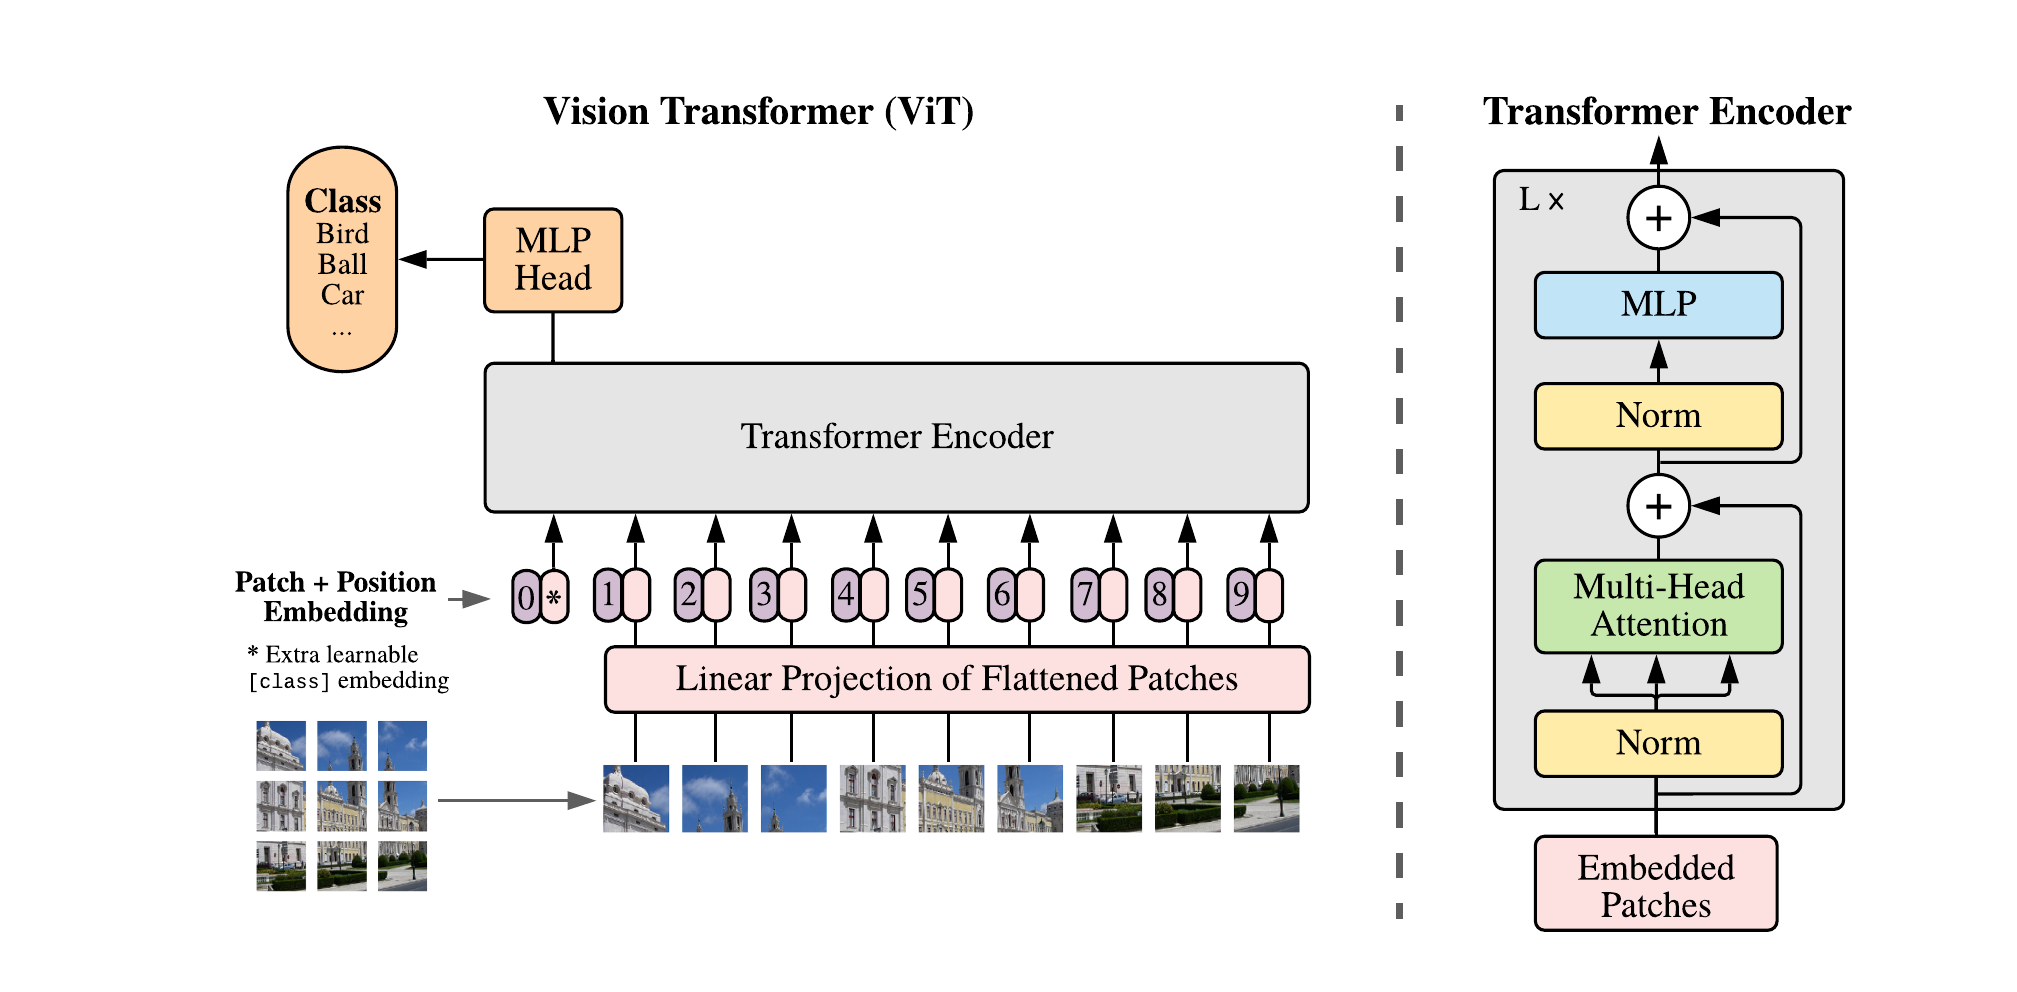
\includegraphics[width=1.0\textwidth]{Chapters/4. ViT-Lung/images/ViT.png}}
\caption{Representación original del modelo ViT mostrado en \cite{DBLP:journals/corr/abs-2010-11929}.
Las imágenes a procesarse son descompuestas en una serie de parches (3x3 parches en este ejemplo). Los
parches generados son proyectados a una dimension linear agregándose información posicional.}
\label{fig_ViT}
\end{figure}

El mecanismo de atención en el modelo ViT transforma continuamente los vectores de representación de
los parches de la imagen, incorporando relaciones semánticas entre ellos. Análogamente a como se usa
en el área de Procesamiento de Lenguaje Natural, mientras los vectores avanzan en profundidad en el
modelo Transformer, las relaciones semánticas formadas entre los parches se vuelven más complejas.
Esto reemplaza las características extraídas a través de operaciones convolucionales. Para realizar
estas tareas, el modelo ViT solo utiliza la parte codificadora de la arquitectura general del Transformer,
codificando y extrayendo la información relevante de las imágenes en las etapas de multi-atención.

A pesar de que los enfoques dirigidos con modelos ViT y CNN son diferentes, algunas investigaciones
indican que la representación de la información en capas inferiores es bastante similar, es decir,
convoluciones más internas que guardan características locales y cabezas de atención más profundas
\cite{DBLP:journals/corr/abs-2108-08810}. Aun así, los modelos ViT incorporan más información global
que los modelos CNN en capas inferiores y los \textit{skip connections} influyen más en los modelos
ViT que en los basados en CNN. Además, como describen en su artículo \citeauthor{DBLP:journals/corr/abs-2010-11929},
los modelos ViT se benefician de entrenamientos con conjuntos de datos mucho más grandes en comparación
con los datos necesarios para obtener resultados favorables en CNN.

Basados en las propuestas de \citeauthor{DBLP:journals/corr/abs-2010-11929}, la red clasificadora
implementada se deriva de los modelos entrenados que describen. Los modelos se entrenan utilizando
varios conjuntos de datos: el conjunto de datos ILSVRC-2012 de ImageNet, que consta de 1k clases y
1.3 millones de imágenes; el conjunto de datos ImageNet-21k, que contiene 21k clases y 14 millones
de imágenes; y el conjunto de datos JFT, que incluye 18k clases y 303 millones de imágenes de alta
resolución. Estos conjuntos de datos proporcionan una amplia variedad de ejemplos que permiten al
modelo aprender y generalizar eficazmente.


\begin{table}[!ht]
    \centering
    \begin{tabular}{| l | c |}
     \hline
    \textbf{Input size}  & 384 $\times$ 384 \\
    \textbf{Patch size}  & 32 $\times$ 32 \\
    \textbf{Layers}      & 12  \\
    \textbf{Hidden size} & 768 \\
    \textbf{MLP Size}    & 3072 \\
    \textbf{Heads}       & 12 \\
    \textbf{Params}      & 87M \\
     \hline
    \end{tabular}
    \caption{Configuración de la arquitectura del modelo ViT usado. Usa imágenes de tamaño
             $384 \times 384$ con 3 canales correspondientes al modo RGB. En total cuenta con 12
             cabezas de atención y 12 codificadores internos.}
\label{table_ViTBase}
\end{table}

La arquitectura del modelo ViT está basada en las implementaciones de los Transformers
mostrados en \textit{BERT} \cite{DBLP:journals/corr/abs-1810-04805}. Presentan distintas nomenclaturas
para definir el tamaño del modelo generado. En particular, se ha usado en este trabajo la arquitectura
\textit{ViT-Base-patch32-384}. \quotes{Base} hace referencia al modelo base de \textit{BERT},
\quotes{patch32} a la variante que trabaja con parches de tamaño $32 \times 32$ y \quotes{384} a las
dimensiones de las imágenes de entrada al modelo. En la tabla \ref{table_ViTBase} y \ref{table_ViT}
se ejemplifica la arquitectura mencionada; 12 capas codificadoras del Transformer conforman el modelo
ViT, con 12 cabezas de atención con un tamaño de 768 y, finalmente, las componentes MLP de tamaño 3072.

En la red detectora basada en ViT, la etapa clasificadora del modelo \textit{ResNet50} también es
reemplazada con dos capas densas y una operación de \textit{Dropout} intermedia con una probabilidad
del $25\%$, similar al modelo de CNN propuesto anteriormente.


\begin{table}[!ht]
    \centering
    \begin{tabular}{| l|c | c | r |}
    \hline
                 &     Input   &  Output    &  \\
    Layer        &   dimension & dimension  & Parameters \\
    \hline\hline
    ViT     &     3,384,384 &     768 & 87,416,064 \\
    Dense        &     768        &     256      & 196,864    \\
    ReLU         &     256         &     256      & --         \\
    Drop-0.25  &     256         &     256      & --         \\
    Dense        &     256         &     15       &  3,855     \\
    Sigmoid      &     15          &     15       & --         \\
    \hline
    \end{tabular}
    \caption{Arquitectura ViT usada en el modelo propuesto. Las capas densas incluyen el término de bias.
    Drop-0.25 significa una capa de Dropout con una probabilidad de 0.25.}
    \label{table_ViT}
\end{table}

\begin{figure}[htp]
    \centering
    {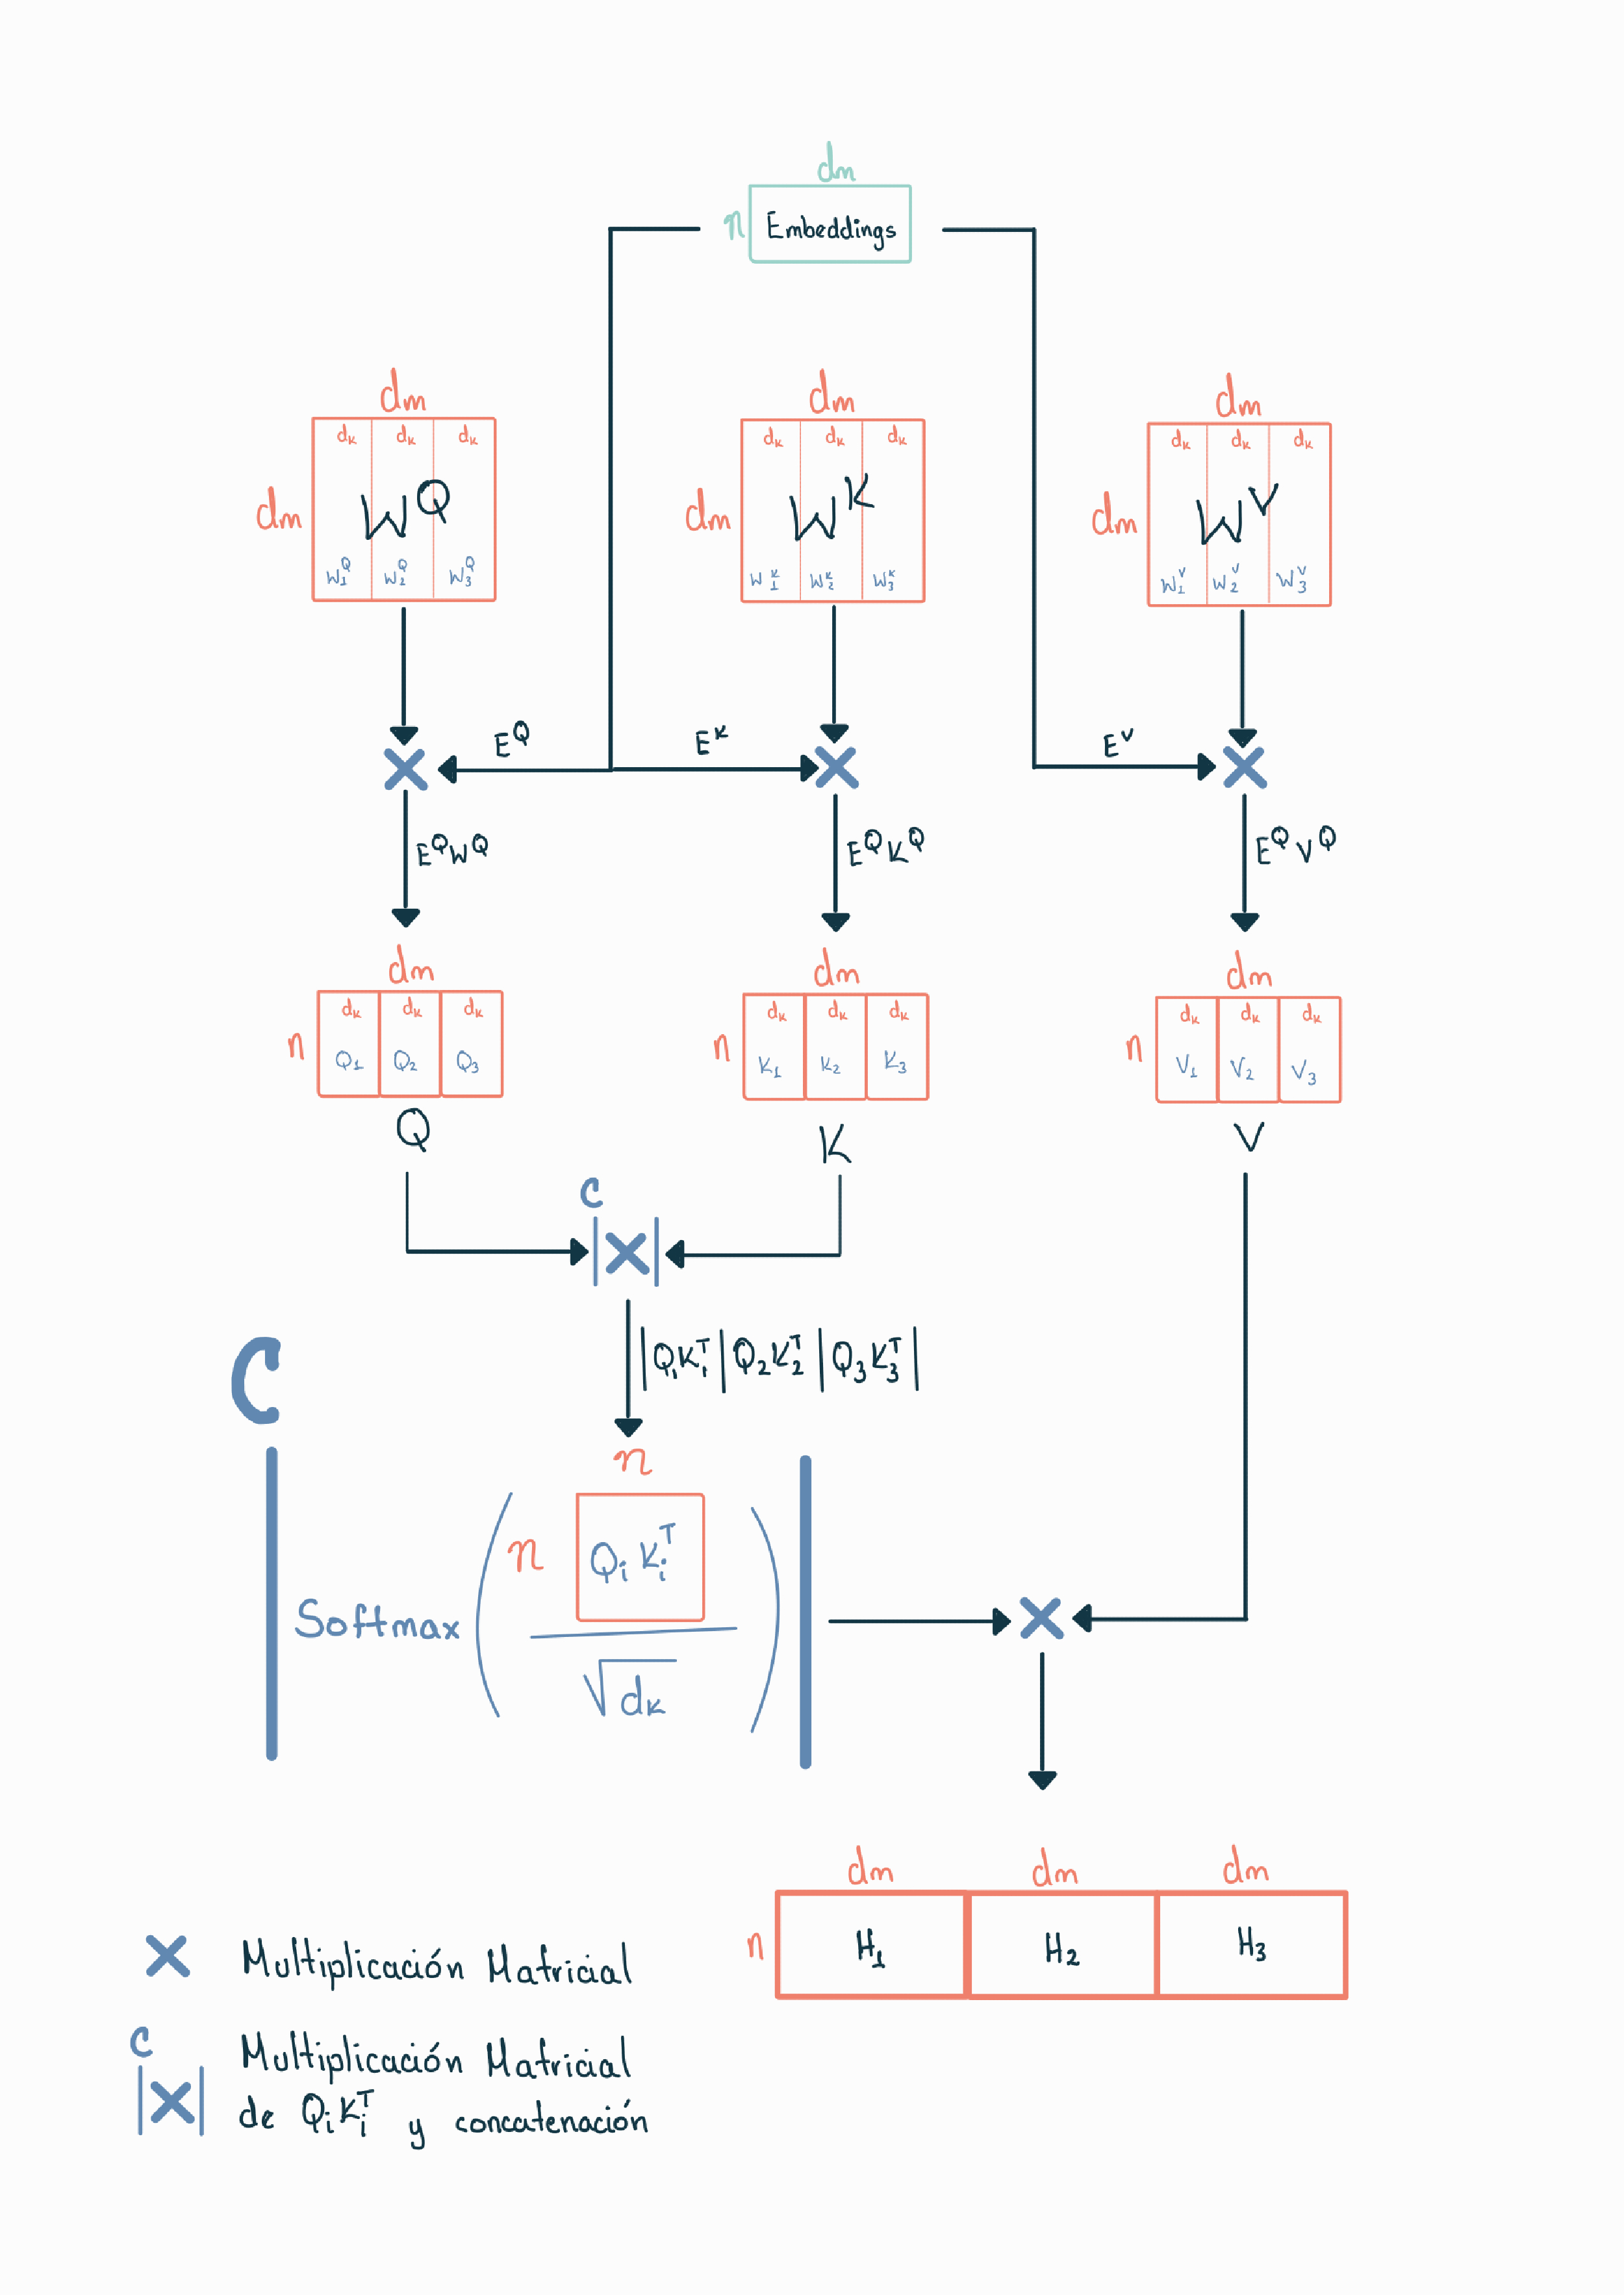
\includegraphics[width=0.7\textwidth]{Chapters/4. ViT-Lung/images/cabezas_vit.jpg}}
\caption{Representación gráfica del módulo de MultiHead Self-Attention en el modelo ViT usando 3 cabezas
         de atención. Se observa
         que el tamaño de la matriz de atención $Q_i K_i^T$ es dependiente del número de parches
         generados en la imagen al igual que el tamaño de cada cabeza de atención $H_i$ depende de
         la dimensión de estos. Las cabezas de atención resultantes finalmente son re-proyectadas
         a dimensiones $n \times d_m$ para las etapas posteriores. }
\label{vit-head-dim}
\end{figure}

% \subsection{ViT con cabezas de atención Flexibles}

% Como se observó en la sección \ref*{section-mha} el Transformer está basado en la idea de
% Multihead-Self-Attention, permitiendo al modelo conjuntamente atender a información en diferentes
% posiciones desde distintos subespacios de representación

% \begin{equation}
%     mha(Q, K, V) = Concat(head_1,head_2,head_3,..., head_h)W^O
% \end{equation}

% con $E_Q, E_K, E_V \in \mathbb{R}^{n \times d_{m}}$ como embeddings de entrada, $n$ es el tamaño de la
% secuencia, $d_m$ es el tamaño del embedding y $h$ el número de cabezas de atención. Cada cabeza de
% atención está indicada como:

% \begin{equation}
%     head_i = Attention(E_Q W_i^Q, E_K W_i^K, E_V W_i^V) =
%     Sofmax\Big(\frac{E_Q W_i^Q (E_K W_i^K)^T}{\sqrt{d_k}}\Big) E_V W_i^V
%     \label{eq:head-mha}
% \end{equation}

% donde $W_i^Q$, $W_i^K$ $\in \mathbb{R}^{d_m \times d_k}$, $W_i^V$ $\in \mathbb{R}^{d_m \times d_v}$,
% $W^O$ $\in \mathbb{R}^{hd_v \times d_m}$ y $d_k=d_v=d_m/h$.

% Observando la ecuación \label{eq:mha} podemos identificar algunas propiedades que se cumplen en el
% modelo de Transformes

% \begin{itemize}
%     \item El tamaño de la cabeza es dependiente de la dimensión del embedding y el número de cabezas
%           de atención.
%     \item Mientras más cabezas de atención los embeddings son proyectados a dimensiones de subespacios
%           de representación cada vez menores, indicando una mayor compresión de la información en estos.
%     \item La necesidad de escalar el modelo implica escalar conjuntamente todas las dimensiones.
% \end{itemize}

% Con ello en mente la hipótesis es que la redefinición de $W_i^Q$, $W_i^K$, $W_i^V$ $\in \mathbb{R}^{d_m \times d_h}$,
% $W^O$ $\in \mathbb{R}^{hd_h \times d_m}$ con $d_h$ como un hiperparámetro y $d_h > d_k$
% podemos tener mayor control de las cabezas de atención y sobre la representación
% del aprendizaje de cada una de ellas.

\subsection{Proceso de Entrenamiento}
\label{ss:archiecture}

% \subsubsection{Proceso de entranamiento para el modelo CNN}

% we present the procedure to train our models to detect the 15 pathology's (including COVID-19) from a network pre-trained with ImageNet.
\begin{enumerate}
    \item \textbf{Entrenamiento inicial}.\\
        \textbf{Modelo CNN}: Una vez seleccionada la red convolucional pre-entrenada con la base de datos de
        ImageNet, se reemplaza la etapa de clasificación por una nueva compuesta por dos capas densas. En la
        tabla \ref{table_resnet50} se presentan los detalles de la red \textit{ResNet50} usada en este modelo.
        De esta forma, la red convolucional \textit{ResNet50} funciona como un extractor de características;
        transforma los datos originales (las imágenes de radiografías) en una nueva representación que contiene
        las características que permiten distinguir entre las distintas patologías. El clasificador se implementa
        agregando dos capas densas a esta red base. En la etapa de entrenamiento, la red se comporta como una red
        Perceptrón Multicapa (\textit{Multilayer Perceptron}, MLP) donde la entrada es el tensor de características
        calculado por la red base o backbone. Para entrenar el clasificador, los pesos que corresponden a la red
        base son congelados y solamente se actualizan los pesos que pertenecen a la etapa de clasificación (las
        capas densas descritas en la tabla \ref{table_resnet50}). El entrenamiento se realiza durante 35 épocas,
        conservando el mejor modelo de acuerdo al \textit{accuracy} obtenido usando el conjunto de validación.

        \textbf{Modelo ViT}: Al igual que el modelo CNN, con la red basada en Transformers y pre-entrenada con la
        base de datos ILSVRC-2012 de ImageNet, se reemplaza la etapa de clasificación por la misma red compuesta
        por dos capas densas. En la tabla \ref{table_ViTBase} y \ref{table_ViT} se presentan los detalles de la
        arquitectura de la red \textit{ViT}. Similar al modelo convolucional, el modelo \textit{ViT} trabaja
        extrayendo características y encontrando relaciones a través de la atención. Esto le permite determinar
        características esenciales para poder identificar las distintas patologías trabajadas. El clasificador
        añadido a la red contiene dos capas densas que procesan la información del modelo ViT y determinan
        finalmente la clasificación correspondiente para cada dato. Durante la primera etapa de entrenamiento,
        los pesos entrenables asociados al modelo \textit{ViT} que conforma la red son congelados, permitiendo
        solo el entrenamiento del modelo clasificador. El entrenamiento se realiza durante 25 épocas,
        conservando el mejor modelo de acuerdo al valor de \textit{accuracy} obtenido usando el conjunto de
        validación.


    \item \textbf{Fine-tuning}\\
        \textbf{Modelo CNN}: Hasta este punto, el enfoque usado es un \textit{aprendizaje superficial} y la
        etapa de extracción de características está completamente desasociada de la etapa de clasificación. La
        ventaja de implementar el sistema a través de dos redes neuronales (la red backbone y la red MLP) es que
        podemos mejorar la extracción de características en términos de la tarea de interés. Para ello, se procede
        a descongelar las últimas capas convolucionales de la red backbone y continuar el entrenamiento en conjunto
        con las capas densas de la etapa clasificadora. Las capas a descongelar corresponden al último bloque
        construido de la 5° etapa convolucional (\textit{layer conv5\_3}) \cite{he2016deep}. Así, permitimos que el
        tensor obtenido a la salida de la red backbone sea particularizado a la tarea de clasificación actual. El
        procedimiento de \textit{Fine-tuning} es realizado por 20 épocas más.\\

        \textbf{Modelo ViT}: Siguiendo un procedimiento similar al modelo propuesto basado en \textit{ResNet50}, se
        procede a descongelar los dos últimos bloques del modelo ViT, esto es, los correspondientes a los bloques 11
        y 12 de acuerdo a la arquitectura vista en la tabla \ref{table_ViT}. Esto permite, de manera similar, que las
        salidas del modelo ViT sean más particulares a la tarea de clasificación en cuestión. 12 épocas más de
        entrenamiento le siguen a este modelo.


    \item \textbf{Full-tuning}\\
        \textbf{Modelo CNN}: Las razones por las cuales solamente son reentrenadas las últimas capas
        convolucionales son que tenemos que lidiar con el problema del desvanecimiento del gradiente y el sistema
        completo puede terminar sobreajustando sus parámetros a la base de datos de entrenamiento. El primer
        problema no es tan relevante en este punto, el rendimiento obtenido por el modelo es satisfactorio y si no
        fuese posible mejorar los parámetros de las capas convolucionales, tampoco sufren un deterioro. El segundo
        problema es de importancia si la muestra de imágenes radiográficas es suficientemente representativa de las
        patologías de interés, puesto que el sistema es suficientemente general para predecir el conjunto de imágenes
        de prueba correctamente. En este trabajo consideramos que tenemos suficientes datos y, por lo tanto, como
        etapa final del entrenamiento se realiza una afinación completa del modelo. Esto es, entrenando completamente
        la red, la etapa de extracción de características (backbone) y la etapa de clasificación (MLP). Para evitar
        el \textit{over-fitting}, el entrenamiento es continuado solamente por 10 épocas, conservando el mejor modelo
        de acuerdo al \textit{accuracy} obtenido en el conjunto de validación.\\

        \textbf{Modelo ViT}: De acuerdo a la premisa anterior, el modelo \textit{ViT} es descongelado completamente,
        permitiendo el entrenamiento de todos los bloques de la red. Esto permite al modelo especializarse en la
        tarea de detección de patologías pulmonares al ajustar sus pesos por algunas épocas más. De la misma manera,
        el modelo \textit{ViT} es entrenado por 8 épocas más. A diferencia del modelo basado en \textit{ResNet50}, el
        número de épocas es menor en cada etapa para el modelo \textit{ViT} puesto que se observó una convergencia
        más rápida.


\end{enumerate}

Similar a \citeauthor{rajpurkar2018deep}, al inicio de cada etapa de entrenamiento en ambas redes,
las imágenes de entrenamiento son volteadas horizontalmente con 0.5 de probabilidad como técnica de
aumento de datos.

La salida de la red basada en \textit{ResNet50} y \textit{ViT} es un vector de tamaño igual al número
de patologías detectadas, 15. Cada elemento del vector $\tilde y_i \in [0,1]$ puede ser interpretado
como la probabilidad de que la i-ésima patología esté presente en la imagen analizada. El vector
$\tilde y$ no necesariamente tiene que sumar 1, puesto que varias patologías pueden estar presentes
en la radiografía. Una patología es detectada como positiva si $\tilde y > \theta$, donde $\theta$ es
el umbral. El valor típico para este umbral es de $0.5$ y puede ser modificado dependiendo del análisis
de la curva del \textit{Receiver Operator Characteristic}, o \textit{Curva ROC}. Como algoritmo de
entrenamiento se usa \emph{Adam} \cite{kingma2017adam} con un factor de aprendizaje (LR) de
$1\times 10^{-4}$ para el modelo basado en \textit{ResNet50} y $1\times 10^{-5}$ para el modelo basado
en \textit{ViT}, con parámetros de inercia $\beta_1=0.9$ y $\beta_2=0.999$ en ambos modelos y con un
decaimiento (LR-decay) de $0.1$ si después de 10 iteraciones no se detecta una reducción en el valor
de la función de pérdida mayor a $1\times 10^{-4}$ (plateau escape).


\subsubsection{Transfer Learning para la detección de Neumonía por Tuberculosis}

El propósito de esta sección es demostrar que el \textit{backbone} del modelo propuesto basado en
\textit{ResNet50} y entrenado con las 15 patologías mencionadas anteriormente, puede ser la base para
desarrollar detectores para otras enfermedades de pulmón. La idea en esta etapa es no repetir el proceso
completo de entrenamiento, sino usar una simple estrategia de \textit{Transfer Learning}. Así, se procede
a extender el modelo para detectar (junto con las otras enfermedades) neumonía causada por Tuberculosis
\cite{stirenko2018chest}, un tipo de neumonía bacteriana común en países en vías de desarrollo y también
frecuentemente reportada en pacientes con síndrome de inmunodeficiencia adquirida (AIDS)
\cite{matsuura2018tuberculous}.


\begin{table}[!ht]
    \centering
    \begin{tabular}{| r |l | c | c | c |}
     \hline
     Class & Disease & Source & Train & Test  \\
     \hline\hline
     16  & Tuberculosis        & 3 & 888   & 488  \\
     ---&  Non-Tuberculosis     & 3 & 6000  & 1600 \\
     \hline
    \end{tabular}
    \caption{ Número de radiografías de tórax de pacientes con y sin Tuberculosis.}
\label{table_dataset_tb}
\end{table}

El dataset considerado incluye casos de \textit{Tuberculosis} y \textit{no Tuberculosis}, pero es
importante aclarar que la condición en particular de los casos de \textit{no Tuberculosis} no está
especificada por completo, es decir, incluyen tanto pacientes saludables como pacientes con otras
afecciones.

La base de datos (indicada proveniente de la fuente 3 en la tabla \ref{table_dataset_tb}) está
compuesta por radiografías provenientes de: TBX11K dataset \cite{liu2020rethinking}, India (DA and DB)
dataset \cite{chauhan2014role}, Montgomery County dataset \cite{jaeger2014two}, y Shenzhen Hospital
dataset \cite{jaeger2014two}. En este trabajo se usan las listas originales para el entrenamiento y
evaluación definidos para este dataset.


\begin{table}[!ht]
    \centering
    \begin{tabular}{| l| c | c | r |}
     \hline
                 &  Input       & Output           &   \\
    Layer        &  dimension    & dimension        & Parameters \\
    \hline\hline
    Initial Backbone & & & \\ \hline
    ResNet50     &  3,1000,1000 &     2048,1,1     & 24,036,431 \\
    Flatten      &     2048     &     2048         &  --        \\
    Dense        &     2048     &     256          & 524,544    \\
    ReLU         &     256      &     256          & --         \\
    Drop-0.25    &     256      &     256          & --         \\
    \hline
    Additional Branch & & & \\ \hline
    Dense$^\ast$ &     256      &     128          &  38,896     \\
    ReLU         &     128      &     128          & --         \\
    Drop-0.20    &     128      &     128          & --         \\
    Dense$^\ast$ &     128      &      1           &  129       \\
    Sigmoid      &      1       &      1           & --         \\
     \hline
    \end{tabular}
    \caption{ Arquitectura del modelo de la red de aprendizaje profundo usada en el modelo extendido
             con una rama para Tuberculosis. Las capas densas incluyen el término de bias y $^\ast$
             indica las capas que son entrenables.}
\label{table_resnet50_tb}
\end{table}

Para poder detectar Tuberculosis, se realiza la implementación de un clasificador binario usando como
\textit{backbone} la red \textit{ResNet50} entrenada previamente para la detección de las 15 patologías
anteriores. La nueva rama de clasificación incluye dos nuevas capas densas (con sus respectivas funciones
de activación). Conservamos los parámetros correspondientes al \textit{backbone} no entrenables y solo se
entrenan las nuevas capas densas usando la estrategia mencionada en la subsección de {\bf Entrenamiento
Inicial} \ref{ss:archiecture} con el optimizador, factor de aprendizaje y otros parámetros sin cambios y
\textit{Weighted Binary Cross-Entropy} como función de pérdida similar a \eqref{eq:loss}. Este modelo
extendido aún detecta las 15 enfermedades comentadas previamente con una salida binaria extra para
Tuberculosis. La arquitectura extendida, incluyendo la nueva rama, está descrita en la tabla
\ref{table_resnet50_tb}.


\begin{figure}[htp]
    \centering
    {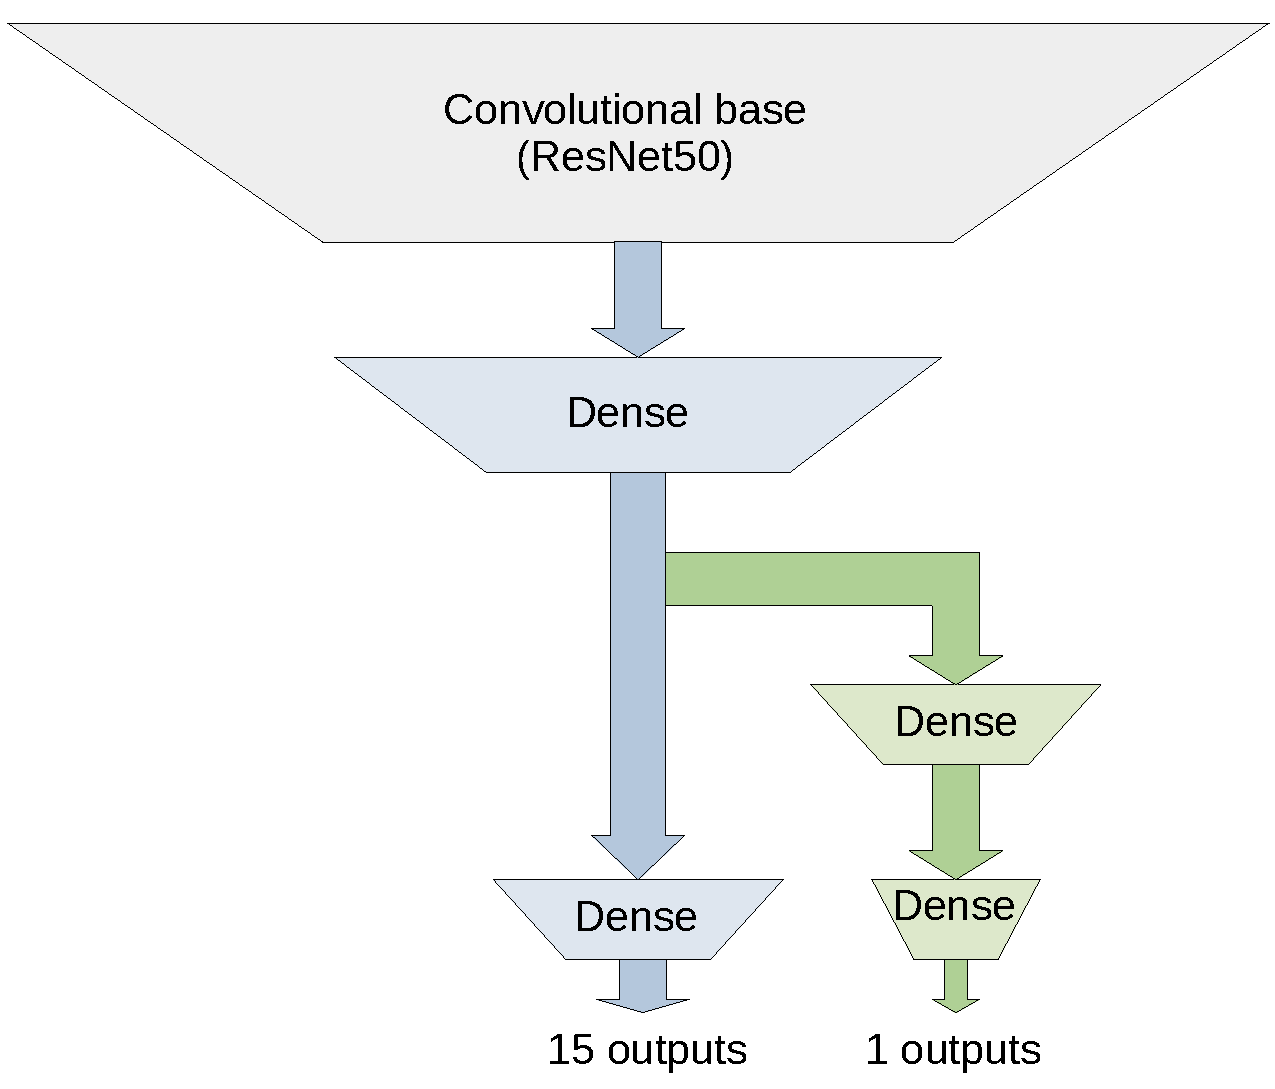
\includegraphics[width=0.5\textwidth]{Chapters/4. ViT-Lung/images/tb_net.pdf}}
\caption{ Esquema de la extensión del detector de las 15 patologías incluyendo una nueva rama para
          la detección de Tuberculosis.}
\label{net_tb}
\end{figure}


\subsection{Métricas de Evaluación} \label{sec_metrics}

Considerando un problema de clasificación binario donde cada radiografía tiene una etiqueta
$y = \{1, 0\}$ con $1$ indicando la presencia del padecimiento en el paciente y $0$ significando
que se encuentra sano, los detectores pueden tener dos posibles resultados: una detección positiva (P)
para la enfermedad o una detección negativa (N). La tabla \ref{table_cm} muestra la caracterización
de la etiqueta predicha de acuerdo a los valores reales (\textit{Ground Truth}, GT). Si un paciente
enfermo es correctamente detectado, tenemos un \textit{Verdadero Positivo} (\textit{True Positive}, TP)
y si la predicción falla, es un \textit{Falso Negativo} (\textit{False Negative}, FN). Por otro lado,
si una etiqueta positiva es erróneamente predicha en un paciente saludable, entonces tenemos un
\textit{Falso Positivo} (\textit{False Positive}, FP), y si el paciente saludable es correctamente
predicho, es un \textit{Verdadero Negativo} (\textit{True Negative}, TN). La tabla \ref{table_cm}
muestra la \textit{Matriz de Confusión} con el conteo de cada tipo de predicción en el conjunto de
prueba.


\begin{table*}[!ht]
    \centering
    \begin{tabular}{ccccl}
    %\cline{3-4}
    &  & \multicolumn{2}{ c }{Predicción} \\
    %\cline{3-4}
    \multicolumn{1}{c}{}& & Positivo & Negativo &    \\
    \cline{3-4}
    \multicolumn{1}{c}{\multirow{6}{*}{GT} } &
    \\
    \multicolumn{1}{c}{} & Enfermo & TP & FN   &  $ \longrightarrow  R = \frac{TP}{TP+FN}$  \\
    \\
    \cline{3-4}
    \multicolumn{1}{ c }{}                    &
    \\
    \multicolumn{1}{c}{} & No-Enfermo & FP & TN   &  $ \longrightarrow S = \frac{TN}{FP+TN}$   \\
    \\
    \cline{3-4}
    \\
    & & $\downarrow$ & $\downarrow$ & \\
    \multicolumn{1}{c}{} &       & $P = \frac{TP}{TP+FP}$  & $NPV = \frac{TN}{FN+TN}$ &
    \end{tabular}
    \caption{Interpretación de los resultados (predicción) de acuerdo al los valores reales (Ground
             Truth, GT). Las métricas son calculadas como la relación entre el elemento de la diagonal
             y la suma correspondiente por fila o por columna. Según sea el caso: R, \textit{recall}
             o \textit{sensitivity}; S, \textit{specificity}; P, \textit{precision}; NPV,
             \textit{negative prediction value}.}
    \label{table_cm}
\end{table*}

Para este trabajo, asumimos que una patología en particular es correctamente detectada si su
correspondiente puntuación en el vector predicho es más significativa que cierto umbral. En particular,
asumimos un umbral igual para todas las patologías de $0.5$ en ambos modelos. Usando la Matriz de
Confusión podemos definir varias métricas de rendimiento.


\begin{enumerate}
    \item Accuracy ($A$). Esta métrica es quizás la más obvia. Corresponde al razón de los datos
          predichos correctamente sobre el total.
    \begin{equation}
        \label{eq:accuracy}
        A = \frac{TP+TN}{TP+TN+FP+FN}.
    \end{equation}

    \item Recall o Sensibility ($R$). Es la fracción de pacientes con enfermedades correctamente
          detectados. Esta métrica también es conocida como Tasa de Verdaderos Positivos (True
          Positive Rate, TPR), la tasa de detecciones correctas.
    \begin{equation}
        \label{eq:TPR}
        R = \frac{TP}{TP + FN}
    \end{equation}

    \item Specificity ($S$). Es la fracción de pacientes sin enfermedades que son detectados
          correctamente.
    \begin{equation}
        \label{eq:Specificity}
        S = \frac{TN}{TN + FP}
    \end{equation}

    \item False Positive Rate ($FPR$). La tasa de detecciones falsas de enfermedades, es calculada
          como:
    \begin{equation}
        \label{eq:FPR}
        FPR = 1 - S,
    \end{equation}
    donde $S$ es el valor de Specificity.

    \item Precision ($P$). Es la fracción de predicciones positivas que realmente tiene una una
          enfermedad.
    \begin{equation}
        \label{eq:P}
        P = \frac{TP}{TP + FP}
    \end{equation}

    \item $F_1$ Score ($F_1$).  Durante la creación de los modelos buscamos un balance entre Precision y
        Recall. El incremento de alguna de estas dos métricas es en compensación de la otra. Un modelo que predice
        la mayoría de los datos como positivos tendrá un \textit{Recall} más cercano a 1, pues el conteo de
        \textit{Falsos Negativos} será mucho menor, pero los \textit{Falsos Positivos} incrementarán, reduciendo
        la \textit{Precision} del modelo. En caso contrario, si el modelo predice la mayoría de los datos como
        negativos, el conteo de \textit{Falsos Positivos} será menor, incrementando la métrica de \textit{Precision},
        pero los \textit{Falsos Negativos} incrementan, provocando que el \textit{Recall} decremente. El
        \textit{F1-Score} busca un balance entre las dos métricas (\textit{Precision-Recall Trade-Off}). Un
        desequilibrio entre ellas indica un sesgo en cualquiera de las dos maneras descritas anteriormente. Por
        ello, es más informativo como medida de rendimiento usar una media geométrica entre las dos métricas.

    \begin{equation}
        \label{eq:f1}
        F_1 = \frac{2\; P \, R}{P + R}.
    \end{equation}

    \item  Area Under Curve of Receiver Operator Characteristic (AUC-ROC). La Curva Característica
        Operativa del Receptor es un gráfico que muestra las capacidades de diagnóstico de clasificadores
        binarios. Como se mencionó anteriormente, una patología es detectada como positiva si su puntaje
        predicho es más significativo que un umbral dado. Así, ajustando dicho umbral a valores más bajos,
        se permite en general incrementar el TPR, aunque el FPR también puede ser incrementado. La Curva ROC
        resulta de graficar los valores de TPR contra FPR variando el umbral en el intervalo $[0,1]$. El AUC
        corresponde al área bajo la Curva de ROC.


\end{enumerate}


\subsection{Resultados}

La Tabla~\ref{table:res-model-covid} y \ref{table:vit-model-covid} muestra un resumen del rendimiento
de los modelos propuestos. Las imágenes que conforman los conjuntos de entrenamiento, validación y prueba
corresponden a los definidos originalmente en el dataset. En \textit{ChestX-ray14}, se redefinen las etiquetas
de entrenamiento de acuerdo a \textit{CheXNet} \cite{rajpurkar2018deep}; excepto para las imágenes de
\textit{COVID-19} y sin patologías identificadas. Es válido usar cualquier modificación de etiquetas en la
etapa de entrenamiento siempre y cuando se mantenga el conjunto de datos de prueba sin cambios (imágenes de
radiografía y sus etiquetas).

Los resultados presentes se ajustan al procedimiento de entrenamiento y prueba antes descrito para ambos
modelos. Las métricas que se incluyen son: \textit{Area Under the Precision Recovery Curve} (AUC-PR),
\textit{Area Under the Receiver Operating Characteristic Curve} (AUC-ROC), \textit{F1-Score} y
\textit{Accuracy} (Acc.). \textit{Global-14} muestra el rendimiento en las patologías de \textit{ChestX-ray-14}
(clasificaciones correctas vs clasificaciones incorrectas), \textit{Global-15} muestra incluyendo
\textit{COVID-19}. Nótese que los modelos propuestos tienen su mejor rendimiento en la detección de
\textit{COVID-19}, la enfermedad anexada. También se han incluido datos de clases sin patologías detectadas
(\textit{healthy}) debido a la importancia de tener un buen desempeño en la detección de sujetos saludables.
El rendimiento global sobre los datos de \textit{ChestX-ray14} y \textit{COVID-19} se muestra en el último
renglón de la tabla \ref{table:res-model-covid} y \ref{table:vit-model-covid}.


\begin{table*}[tb]
    \centering
    \begin{tabular}{|l||c|c|c|c|}
        \hline
    {\bf Patología} 	    	&	\multicolumn{4}{c|}{\bf Modelo propuesto ResNet50}  \\
    \cline{2-5}
                        &	AUC-PR	&	AUC-ROC 	& F1-Score  & Acc.  \\
        \hline \hline
        Cardiomegaly	&	0.290	&	0.875	&	0.324	&	0.911	\\
        Emphysema	    &	0.413	&	0.938	&	0.350	&	0.886	\\
        Effusion	    &	0.494	&	0.850	&	0.527	&	0.807	\\
        Hernia	        &	0.050	&	0.855	&	0.051	&	0.957	\\
        Infiltration	&	0.382	&	0.740	&	0.458	&	0.711	\\
        Mass	        &	0.290	&	0.831	&	0.340	&	0.877	\\
        Nodule	        &	0.249	&	0.806	&	0.299	&	0.876	\\
        Atelectasis	    &	0.336	&	0.794	&	0.387	&	0.815	\\
        Pneumothorax	&	0.447	&	0.906	&	0.496	&	0.852	\\
        Pleural-Thick	&	0.157	&	0.820	&	0.217	&	0.852	\\
        Pneumonia	    &	0.425	&	0.863	&	0.274	&	0.856	\\
        Fibrosis	    &	0.106	&	0.852	&	0.154	&	0.910	\\
        Edema	        &	0.187	&	0.879	&	0.193	&	0.788	\\
        Consolidation	&	0.150	&	0.776	&	0.234	&	0.754	\\
        \hline
        COVID-19	    &	0.844	&	0.991	&	0.799	&	0.969	\\
        Healthy	        &	0.691	&	0.736	&	0.496	&	0.712	\\
        \hline\hline
        Global-14	    &	0.284	&	0.842	&	0.307	&	0.847	\\
        Global-15	    &	0.321	&	0.852	&	0.340	&	0.855	\\
    \hline
    \end{tabular}
    \caption{Resumen del rendimiento del modelo propuesto basado en \textit{ResNet50}.
            Los conjuntos de datos de validación corresponden a como originalmente
            están definidos en ChestX-ray14. Los etiquetas de entrenamiento corresponden a las
            definidas de acuerdo al re-etiquetado realizado por CheXNet; véase \cite{rajpurkar2018deep}
            El valor de umbral está definido igual a 0.5. Ninguna otra optimización fue realizada.}
    \label{table:res-model-covid}
\end{table*}

\begin{table*}[tb]
    \centering
    \begin{tabular}{|l||c|c|c|c|}
        \hline
    {\bf Patología} 	    	&	\multicolumn{4}{c|}{\bf Modelo propuesto ViT}  \\
    \cline{2-5}
                        &	AUC-PR	&	AUC-ROC 	& F1-Score  & Acc.  \\
        \hline \hline
        Cardiomegaly	&	0.253	&	0.866	&	0.324	&	0.928	\\
        Emphysema	    &	0.246	&	0.866	&	0.319	&	0.924	\\
        Effusion	    &	0.401	&	0.791	&	0.434	&	0.807	\\
        Hernia	        &	0.036	&	0.843	&	0.064	&	0.971	\\
        Infiltration	&	0.256	&	0.621	&	0.235	&	0.724	\\
        Mass	        &	0.227	&	0.768	&	0.296	&	0.900	\\
        Nodule	        &	0.157	&	0.704	&	0.209	&	0.908	\\
        Atelectasis	    &	0.271	&	0.734	&	0.325	&	0.840	\\
        Pneumothorax	&	0.359	&	0.842	&	0.430	&	0.880	\\
        Pleural-Thick	&	0.125	&	0.765	&	0.197	&	0.881	\\
        Pneumonia	    &	0.104	&	0.738	&	0.144	&	0.732	\\
        Fibrosis	    &	0.070	&	0.810	&	0.134	&	0.932	\\
        Edema	        &	0.120	&	0.828	&	0.180	&	0.877	\\
        Consolidation	&	0.118	&	0.715	&	0.171	&	0.836	\\
        \hline
        COVID-19	    &	0.859	&	0.982	&	0.801	&	0.973	\\
        Healthy	        &	0.634	&	0.705	&	0.537	&	0.703	\\
        \hline\hline
        Global-14	    &	0.196	&	0.778	&	0.247	&	0.867	\\
        Global-15	    &	0.240	&	0.791	&	0.284	&	0.874	\\
    \hline
    \end{tabular}
    \caption{Resumen del rendimiento del modelo propuesto basado en \textit{ViT}.
            Los conjuntos de datos de validación corresponden a como originalmente
            están definidos en ChestX-ray14. Los etiquetas de entrenamiento corresponden a las
            definidas de acuerdo al re-etiquetado realizado por CheXNet; véase \cite{rajpurkar2018deep}
            El valor de umbral está definido igual a 0.5. Ninguna otra optimización fue realizada.}
    \label{table:vit-model-covid}
\end{table*}

Es importante recalcar que no es apropiado usar \textit{Accuracy} como único criterio de rendimiento
bajo este contexto. El \textit{Accuracy} de cada clase es calculado como el número de clasificaciones
correctas (TP y TN) entre la suma total de radiografías analizadas. Con clases desbalanceadas, tales
como las que analizamos ahora (patología vs no patología), un modelo podría ser engañoso en cuanto a
su eficiencia, sesgando su clasificación sobre la o las clases más representativas. Si el desbalance
es grande, el modelo puede asignar todos los datos como la clase que representa mayor peso y, por tanto,
tener un buen rendimiento en la métrica de \textit{Accuracy}. A pesar de ello, los datos presentados
son resultados que sirven como referencia para el lector. Una manera más apropiada de medir el desempeño
del modelo es calcular la gráfica de TPR vs FPR para obtener el área bajo la curva, en otras palabras,
calcular AUC-ROC como la métrica de rendimiento \cite{Hanley1983-tu}. A pesar de que la curva de ROC
es preferida sobre la de PR a causa de su convexidad, existe un mapeo uno a uno entre ellas
\cite{10.1145/1143844.1143874}. Al final, ambas curvas son calculadas usando la misma matriz de
confusión. Por tanto, también se incluye la métrica AUC-PR para comparaciones más informativas que
solo usar la curva de ROC \cite{Saito2015-db}.


La tabla \ref{table_roc_auc} muestra una comparación de la métrica AUC-ROC para los modelos DR-CNN
\cite{DBLP:journals/corr/abs-1808-05744}, CRAL \cite{GUAN2020259}, TSNC \cite{CHEN2020221}, CheXNet
\cite{rajpurkar2018deep} y las dos propuestas descritas aquí, el modelo basado en ViT y el modelo basado
en ResNet50. También se realiza la comparativa del modelo ResNet-38-large-meta (LargeMeta). Este modelo
emplea ResNet-38 como \textit{backbone}, un tamaño de imagen de $480 \times 480$ píxeles y, a diferencia
de los modelos comparados restantes, utiliza datos adjuntos a la imagen (metadata). Las tres últimas
columnas presentan la AUC-ROC para los modelos propuestos y la detección lograda por un grupo de radiólogos
\cite{rajpurkar2018deep}. Se indica en negritas el modelo con el mejor rendimiento por patología.

En general, la métrica AUC-ROC en el dataset original \textit{ChestX-ray14} muestra una ligera ventaja
para el modelo propuesto basado en \textit{ResNet50} sobre el modelo \textit{CheXNet}. La inclusión de
\textit{COVID-19} mejora dicha métrica de rendimiento en favor del modelo propuesto. Además, es visible
que los resultados obtenidos también superan a aquellos reportados por otros métodos investigados en
\cite{baltruschat2019comparison}. Es importante notar que la métrica AUC-ROC para \textit{CheXNet}
corresponde a la media de 1000 salidas usando \textit{boostraping} para un Intervalo de Confianza del
$95\%$ \cite{rajpurkar2018deep}. Una actualización reciente de la implementación de \textit{CheXNet} en
el repositorio \cite{chexnet_code} reporta un AUC-ROC para \textit{Global-14} igual a 0.847. La última
columna en la \ref{table_roc_auc} presenta el rendimiento promedio para los radiólogos que evalúan la radiografía
para \textit{ChestX-ray14}. Para mayor detalle del cómputo de la evaluación de los radiólogos, véase
\cite{rajpurkar2018deep}. Las marcas con asterisco $(*)$ indican donde los radiólogos tienen mejor
rendimiento que cualquiera de los modelos evaluados. La tabla \ref{table_dl_human} resume el rendimiento
de la métrica AUC-ROC de los mejores métodos basados en DL (incluyendo el propio analizado basado en
\textit{ResNet50}) contra el rendimiento de los radiólogos. Podemos notar una ventaja si unimos los
métodos basados en DL, los cuales superan a los radiólogos en detectar seis patologías (sin tomar en
cuenta \textit{COVID-19}).


\begin{table*}[tb]
    \centering
    %\resizebox{\textwidth}{!}{
    \begin{tabular}{|l||c|c|c|c|c|c|c|l|}
        \hline
        \multicolumn{1}{|c||}{Patología}	&	\multicolumn{5}{c|}{\bf Modelos comparativos}    &\multicolumn{2}{c|}{\bf Propuestas} & 	\\
        \cline{2-9}
                        &	CRAL	&	DR-CNN	&	TSNC	& LgMeta & CheXNet	& CNN	    & ViT & 	Radiol.	\\
        \hline\hline
        Cardiomegaly	&	0.880	&	0.801	&	0.887	&	0.875	&\bf{0.923}	&	0.875	& 0.866 &	0.888	\\
        Emphysema	    &	0.908	&	0.773	&	0.930	&	0.895	&	0.937	&\bf{0.938}	& 0.866 &   0.911	\\
        Effusion	    &	0.829	&	0.797	&	0.831	&	0.822	&\bf{0.864}	&	0.850	& 0.791 &   0.900*	\\
        Hernia	        &	0.917	&	0.748	&	0.921	&\bf{0.937}	&	0.916	&	0.855	& 0.843 &   0.985*	\\
        Infiltration	&	0.702	&\bf{0.751}	&	0.703	&	0.694	&	0.734	&	0.740	& 0.621 &	0.734	\\
        Mass	        &	0.834	&	0.760	&	0.833	&	0.820	&\bf{0.868}	&	0.831	& 0.768 &	0.886*	\\
        Nodule	        &	0.773	&	0.741	&	0.798	&	0.747	&	0.780	&\bf{0.806}	& 0.704 &	0.899*	\\
        Atelectasis	    &	0.781	&	0.766	&	0.785	&	0.763	&\bf{0.809}	&	0.794	& 0.734 &	0.808	\\
        Pneumothorax	&	0.729	&	0.778	&	0.731	&	0.840	&	0.889	&\bf{0.906}	& 0.842 &	0.940*	\\
        Pleural-Thick.	&	0.778	&	0.759	&	0.782	&	0.763	&	0.806	&\bf{0.820}	& 0.765 &	0.779	\\
        Pneumonia	    &	0.857	&	0.800	&\bf{0.881}	&	0.731	&	0.768	&	0.863	& 0.738 &	0.823	\\
        Fibrosis	    &	0.830	&	0.765	&	0.833	&	0.816	&	0.805	&\bf{0.852}	& 0.810 &	0.897*	\\
        Edema	        &	0.850	&	0.820	&	0.849	&	0.846	&\bf{0.888}	&	0.879	& 0.828 &	0.910*	\\
        Consolidation	&	0.754	&	0.787	&	0.754	&	0.749	&\bf{0.790}	&	0.776	& 0.715 &	0.841*	\\
        \hline
        COVID-19	    &	---	    &	---	    &	---	    &	---	    &	---	    &\bf{0.991}	& 0.982 &	---	    \\
        Healthy	        &	---	    &	---	    &	---	    &	0.727	&	---	    &\bf{0.736}	& 0.705 &	---	    \\
        \hline\hline
        Global-14	    &	0.816	&	0.775	&	0.823	&	0.807	&	0.841	&\bf{0.842}	& 0.778 &	0.872*	\\
        Global-15	    &	---	    &	---	    &	---	    &	---	    &	---	    &\bf{0.852}	& 0.791 &	---	    \\
        \hline
    \end{tabular}
    %}
    \caption{Valores correspondientes a la métrica AUC-ROC para las 15 patologías y muestras saludables.
             Los modelos usados en la comparación fueron entrenados para detectar las 14 patologías
             en ChestX-ray14.}
    \label{table_roc_auc}
\end{table*}


\begin{table}[tb]
    \centering
    %\resizebox{\textwidth}{!}{
    \begin{tabular}{|l||l|c|l|}
        \hline
                        &	Method	&	AUC-ROC	& Radiol.	\\
        \hline\hline
        Cardiomegaly	&	CheXNet	    & 0.923 &   0.888	\\
        Emphysema	    &	Proposal    & 0.938	&   0.911	\\
        Effusion	    &	CheXNet	    & 0.864 &   0.900*	\\
        Hernia	        &	LargeMeta   & 0.937	&   0.985*	\\
        Infiltration	&	DR-CNN	    & 0.751 &	0.734	\\
        Mass	        &	CheXNet	    & 0.868	&	0.886*	\\
        Nodule	        &	Proposal    & 0.806	&	0.899*	\\
        Atelectasis	    &	CheXNet	    & 0.809 &	0.808	\\
        Pneumothorax	&	Proposal    & 0.906 &	0.940*	\\
        Pleural-Thick.	&	Proposal    & 0.820	&	0.779	\\
        Pneumonia	    &	TSNC	    & 0.881 &	0.823	\\
        Fibrosis	    &	Proposal    & 0.852 &	0.897*	\\
        Edema	        &	CheXNet	    & 0.888 &	0.910*	\\
        Consolidation	&	CheXNet	    & 0.790 &	0.841*	\\
        COVID-19	    &	Proposal    & 0.991 &	------	\\
        \hline
    \end{tabular}
    %}
    \caption{Comparativo por patología de los modelos de deep learning con mejor rendimiento contra
             el rendimiento de los radiólogos humanos.Los radiólogos lideran en 8 de las 15
             patologías.}
    \label{table_dl_human}
\end{table}


La figura \ref{roc-curves-cnn} y \ref{roc-curves-vit} representan las curvas de ROC correspondientes
a las propuestas basadas en \textit{ResNet50} y \textit{ViT} respectivamente, de todas las patologías
incluyendo las clases \textit{COVID-19} y \textit{Healthy}. Como puede verse en cada uno de los
gráficos, las curvas se encuentran sobre la diagonal, en particular para \textit{COVID-19}. La figura
\ref{img-results} ilustra la detección obtenida mediante el método propuesto: un diagnóstico previo
y la región de interés detectada usando \textit{GradCAM}; una técnica de visualización de redes neuronales
profundas propuesta en \cite{selvaraju2017grad}. La primera fila muestra cuatro radiografías de
pacientes con diferentes patologías, en la segunda fila se encuentra su correspondiente \textit{GradCAM}
indicando la región que contribuye a la detección. Las imágenes radiográficas de la figura están
correctamente clasificadas de acuerdo con las etiquetas originales. Las regiones rojas son aquellas
con mayor contribución a la detección de la enfermedad. La radiografía de la primera columna claramente
muestra un corazón de tamaño mayor de lo normal. La segunda columna corresponde a neumonía, la
tercera columna muestra una formación inusual en el pulmón (\textit{mass}), y la última columna indica
el caso de \textit{COVID-19}. A su vez, se muestran imágenes de las radiografías correspondientes a cada
una de las 15 patologías en las figuras \ref{fig-atelectasis} a \ref{fig-ntorx}. En estas se observa
la imagen radiográfica original de los pulmones, así como el \textit{GradCAM} correspondiente de la
detección del clasificador basado en \textit{ResNet50} y cuya predicción fue positiva a la enfermedad
en cuestión.


\begin{figure}
    \begin{center}
        \scalebox{0.6}{%% Creator: Matplotlib, PGF backend
%%
%% To include the figure in your LaTeX document, write
%%   \input{<filename>.pgf}
%%
%% Make sure the required packages are loaded in your preamble
%%   \usepackage{pgf}
%%
%% Figures using additional raster images can only be included by \input if
%% they are in the same directory as the main LaTeX file. For loading figures
%% from other directories you can use the `import` package
%%   \usepackage{import}
%%
%% and then include the figures with
%%   \import{<path to file>}{<filename>.pgf}
%%
%% Matplotlib used the following preamble
%%
\begingroup%
\makeatletter%
\begin{pgfpicture}%
\pgfpathrectangle{\pgfpointorigin}{\pgfqpoint{10.000000in}{10.000000in}}%
\pgfusepath{use as bounding box, clip}%
\begin{pgfscope}%
\pgfsetbuttcap%
\pgfsetmiterjoin%
\pgfsetlinewidth{0.000000pt}%
\definecolor{currentstroke}{rgb}{1.000000,1.000000,1.000000}%
\pgfsetstrokecolor{currentstroke}%
\pgfsetstrokeopacity{0.000000}%
\pgfsetdash{}{0pt}%
\pgfpathmoveto{\pgfqpoint{0.000000in}{0.000000in}}%
\pgfpathlineto{\pgfqpoint{10.000000in}{0.000000in}}%
\pgfpathlineto{\pgfqpoint{10.000000in}{10.000000in}}%
\pgfpathlineto{\pgfqpoint{0.000000in}{10.000000in}}%
\pgfpathclose%
\pgfusepath{}%
\end{pgfscope}%
\begin{pgfscope}%
\pgfsetbuttcap%
\pgfsetmiterjoin%
\definecolor{currentfill}{rgb}{1.000000,1.000000,1.000000}%
\pgfsetfillcolor{currentfill}%
\pgfsetlinewidth{0.000000pt}%
\definecolor{currentstroke}{rgb}{0.000000,0.000000,0.000000}%
\pgfsetstrokecolor{currentstroke}%
\pgfsetstrokeopacity{0.000000}%
\pgfsetdash{}{0pt}%
\pgfpathmoveto{\pgfqpoint{0.763041in}{8.027083in}}%
\pgfpathlineto{\pgfqpoint{2.450346in}{8.027083in}}%
\pgfpathlineto{\pgfqpoint{2.450346in}{9.566628in}}%
\pgfpathlineto{\pgfqpoint{0.763041in}{9.566628in}}%
\pgfpathclose%
\pgfusepath{fill}%
\end{pgfscope}%
\begin{pgfscope}%
\pgfsetbuttcap%
\pgfsetroundjoin%
\definecolor{currentfill}{rgb}{0.000000,0.000000,0.000000}%
\pgfsetfillcolor{currentfill}%
\pgfsetlinewidth{0.803000pt}%
\definecolor{currentstroke}{rgb}{0.000000,0.000000,0.000000}%
\pgfsetstrokecolor{currentstroke}%
\pgfsetdash{}{0pt}%
\pgfsys@defobject{currentmarker}{\pgfqpoint{0.000000in}{-0.048611in}}{\pgfqpoint{0.000000in}{0.000000in}}{%
\pgfpathmoveto{\pgfqpoint{0.000000in}{0.000000in}}%
\pgfpathlineto{\pgfqpoint{0.000000in}{-0.048611in}}%
\pgfusepath{stroke,fill}%
}%
\begin{pgfscope}%
\pgfsys@transformshift{0.839736in}{8.027083in}%
\pgfsys@useobject{currentmarker}{}%
\end{pgfscope}%
\end{pgfscope}%
\begin{pgfscope}%
\definecolor{textcolor}{rgb}{0.000000,0.000000,0.000000}%
\pgfsetstrokecolor{textcolor}%
\pgfsetfillcolor{textcolor}%
\pgftext[x=0.839736in,y=7.929861in,,top]{\color{textcolor}\rmfamily\fontsize{10.000000}{12.000000}\selectfont \(\displaystyle {0.0}\)}%
\end{pgfscope}%
\begin{pgfscope}%
\pgfsetbuttcap%
\pgfsetroundjoin%
\definecolor{currentfill}{rgb}{0.000000,0.000000,0.000000}%
\pgfsetfillcolor{currentfill}%
\pgfsetlinewidth{0.803000pt}%
\definecolor{currentstroke}{rgb}{0.000000,0.000000,0.000000}%
\pgfsetstrokecolor{currentstroke}%
\pgfsetdash{}{0pt}%
\pgfsys@defobject{currentmarker}{\pgfqpoint{0.000000in}{-0.048611in}}{\pgfqpoint{0.000000in}{0.000000in}}{%
\pgfpathmoveto{\pgfqpoint{0.000000in}{0.000000in}}%
\pgfpathlineto{\pgfqpoint{0.000000in}{-0.048611in}}%
\pgfusepath{stroke,fill}%
}%
\begin{pgfscope}%
\pgfsys@transformshift{1.606693in}{8.027083in}%
\pgfsys@useobject{currentmarker}{}%
\end{pgfscope}%
\end{pgfscope}%
\begin{pgfscope}%
\definecolor{textcolor}{rgb}{0.000000,0.000000,0.000000}%
\pgfsetstrokecolor{textcolor}%
\pgfsetfillcolor{textcolor}%
\pgftext[x=1.606693in,y=7.929861in,,top]{\color{textcolor}\rmfamily\fontsize{10.000000}{12.000000}\selectfont \(\displaystyle {0.5}\)}%
\end{pgfscope}%
\begin{pgfscope}%
\pgfsetbuttcap%
\pgfsetroundjoin%
\definecolor{currentfill}{rgb}{0.000000,0.000000,0.000000}%
\pgfsetfillcolor{currentfill}%
\pgfsetlinewidth{0.803000pt}%
\definecolor{currentstroke}{rgb}{0.000000,0.000000,0.000000}%
\pgfsetstrokecolor{currentstroke}%
\pgfsetdash{}{0pt}%
\pgfsys@defobject{currentmarker}{\pgfqpoint{0.000000in}{-0.048611in}}{\pgfqpoint{0.000000in}{0.000000in}}{%
\pgfpathmoveto{\pgfqpoint{0.000000in}{0.000000in}}%
\pgfpathlineto{\pgfqpoint{0.000000in}{-0.048611in}}%
\pgfusepath{stroke,fill}%
}%
\begin{pgfscope}%
\pgfsys@transformshift{2.373650in}{8.027083in}%
\pgfsys@useobject{currentmarker}{}%
\end{pgfscope}%
\end{pgfscope}%
\begin{pgfscope}%
\definecolor{textcolor}{rgb}{0.000000,0.000000,0.000000}%
\pgfsetstrokecolor{textcolor}%
\pgfsetfillcolor{textcolor}%
\pgftext[x=2.373650in,y=7.929861in,,top]{\color{textcolor}\rmfamily\fontsize{10.000000}{12.000000}\selectfont \(\displaystyle {1.0}\)}%
\end{pgfscope}%
\begin{pgfscope}%
\definecolor{textcolor}{rgb}{0.000000,0.000000,0.000000}%
\pgfsetstrokecolor{textcolor}%
\pgfsetfillcolor{textcolor}%
\pgftext[x=1.606693in,y=7.750849in,,top]{\color{textcolor}\rmfamily\fontsize{16.000000}{19.200000}\selectfont FPR}%
\end{pgfscope}%
\begin{pgfscope}%
\pgfsetbuttcap%
\pgfsetroundjoin%
\definecolor{currentfill}{rgb}{0.000000,0.000000,0.000000}%
\pgfsetfillcolor{currentfill}%
\pgfsetlinewidth{0.803000pt}%
\definecolor{currentstroke}{rgb}{0.000000,0.000000,0.000000}%
\pgfsetstrokecolor{currentstroke}%
\pgfsetdash{}{0pt}%
\pgfsys@defobject{currentmarker}{\pgfqpoint{-0.048611in}{0.000000in}}{\pgfqpoint{-0.000000in}{0.000000in}}{%
\pgfpathmoveto{\pgfqpoint{-0.000000in}{0.000000in}}%
\pgfpathlineto{\pgfqpoint{-0.048611in}{0.000000in}}%
\pgfusepath{stroke,fill}%
}%
\begin{pgfscope}%
\pgfsys@transformshift{0.763041in}{8.097062in}%
\pgfsys@useobject{currentmarker}{}%
\end{pgfscope}%
\end{pgfscope}%
\begin{pgfscope}%
\definecolor{textcolor}{rgb}{0.000000,0.000000,0.000000}%
\pgfsetstrokecolor{textcolor}%
\pgfsetfillcolor{textcolor}%
\pgftext[x=0.418904in, y=8.048837in, left, base]{\color{textcolor}\rmfamily\fontsize{10.000000}{12.000000}\selectfont \(\displaystyle {0.00}\)}%
\end{pgfscope}%
\begin{pgfscope}%
\pgfsetbuttcap%
\pgfsetroundjoin%
\definecolor{currentfill}{rgb}{0.000000,0.000000,0.000000}%
\pgfsetfillcolor{currentfill}%
\pgfsetlinewidth{0.803000pt}%
\definecolor{currentstroke}{rgb}{0.000000,0.000000,0.000000}%
\pgfsetstrokecolor{currentstroke}%
\pgfsetdash{}{0pt}%
\pgfsys@defobject{currentmarker}{\pgfqpoint{-0.048611in}{0.000000in}}{\pgfqpoint{-0.000000in}{0.000000in}}{%
\pgfpathmoveto{\pgfqpoint{-0.000000in}{0.000000in}}%
\pgfpathlineto{\pgfqpoint{-0.048611in}{0.000000in}}%
\pgfusepath{stroke,fill}%
}%
\begin{pgfscope}%
\pgfsys@transformshift{0.763041in}{8.446959in}%
\pgfsys@useobject{currentmarker}{}%
\end{pgfscope}%
\end{pgfscope}%
\begin{pgfscope}%
\definecolor{textcolor}{rgb}{0.000000,0.000000,0.000000}%
\pgfsetstrokecolor{textcolor}%
\pgfsetfillcolor{textcolor}%
\pgftext[x=0.418904in, y=8.398734in, left, base]{\color{textcolor}\rmfamily\fontsize{10.000000}{12.000000}\selectfont \(\displaystyle {0.25}\)}%
\end{pgfscope}%
\begin{pgfscope}%
\pgfsetbuttcap%
\pgfsetroundjoin%
\definecolor{currentfill}{rgb}{0.000000,0.000000,0.000000}%
\pgfsetfillcolor{currentfill}%
\pgfsetlinewidth{0.803000pt}%
\definecolor{currentstroke}{rgb}{0.000000,0.000000,0.000000}%
\pgfsetstrokecolor{currentstroke}%
\pgfsetdash{}{0pt}%
\pgfsys@defobject{currentmarker}{\pgfqpoint{-0.048611in}{0.000000in}}{\pgfqpoint{-0.000000in}{0.000000in}}{%
\pgfpathmoveto{\pgfqpoint{-0.000000in}{0.000000in}}%
\pgfpathlineto{\pgfqpoint{-0.048611in}{0.000000in}}%
\pgfusepath{stroke,fill}%
}%
\begin{pgfscope}%
\pgfsys@transformshift{0.763041in}{8.796856in}%
\pgfsys@useobject{currentmarker}{}%
\end{pgfscope}%
\end{pgfscope}%
\begin{pgfscope}%
\definecolor{textcolor}{rgb}{0.000000,0.000000,0.000000}%
\pgfsetstrokecolor{textcolor}%
\pgfsetfillcolor{textcolor}%
\pgftext[x=0.418904in, y=8.748630in, left, base]{\color{textcolor}\rmfamily\fontsize{10.000000}{12.000000}\selectfont \(\displaystyle {0.50}\)}%
\end{pgfscope}%
\begin{pgfscope}%
\pgfsetbuttcap%
\pgfsetroundjoin%
\definecolor{currentfill}{rgb}{0.000000,0.000000,0.000000}%
\pgfsetfillcolor{currentfill}%
\pgfsetlinewidth{0.803000pt}%
\definecolor{currentstroke}{rgb}{0.000000,0.000000,0.000000}%
\pgfsetstrokecolor{currentstroke}%
\pgfsetdash{}{0pt}%
\pgfsys@defobject{currentmarker}{\pgfqpoint{-0.048611in}{0.000000in}}{\pgfqpoint{-0.000000in}{0.000000in}}{%
\pgfpathmoveto{\pgfqpoint{-0.000000in}{0.000000in}}%
\pgfpathlineto{\pgfqpoint{-0.048611in}{0.000000in}}%
\pgfusepath{stroke,fill}%
}%
\begin{pgfscope}%
\pgfsys@transformshift{0.763041in}{9.146752in}%
\pgfsys@useobject{currentmarker}{}%
\end{pgfscope}%
\end{pgfscope}%
\begin{pgfscope}%
\definecolor{textcolor}{rgb}{0.000000,0.000000,0.000000}%
\pgfsetstrokecolor{textcolor}%
\pgfsetfillcolor{textcolor}%
\pgftext[x=0.418904in, y=9.098527in, left, base]{\color{textcolor}\rmfamily\fontsize{10.000000}{12.000000}\selectfont \(\displaystyle {0.75}\)}%
\end{pgfscope}%
\begin{pgfscope}%
\pgfsetbuttcap%
\pgfsetroundjoin%
\definecolor{currentfill}{rgb}{0.000000,0.000000,0.000000}%
\pgfsetfillcolor{currentfill}%
\pgfsetlinewidth{0.803000pt}%
\definecolor{currentstroke}{rgb}{0.000000,0.000000,0.000000}%
\pgfsetstrokecolor{currentstroke}%
\pgfsetdash{}{0pt}%
\pgfsys@defobject{currentmarker}{\pgfqpoint{-0.048611in}{0.000000in}}{\pgfqpoint{-0.000000in}{0.000000in}}{%
\pgfpathmoveto{\pgfqpoint{-0.000000in}{0.000000in}}%
\pgfpathlineto{\pgfqpoint{-0.048611in}{0.000000in}}%
\pgfusepath{stroke,fill}%
}%
\begin{pgfscope}%
\pgfsys@transformshift{0.763041in}{9.496649in}%
\pgfsys@useobject{currentmarker}{}%
\end{pgfscope}%
\end{pgfscope}%
\begin{pgfscope}%
\definecolor{textcolor}{rgb}{0.000000,0.000000,0.000000}%
\pgfsetstrokecolor{textcolor}%
\pgfsetfillcolor{textcolor}%
\pgftext[x=0.418904in, y=9.448424in, left, base]{\color{textcolor}\rmfamily\fontsize{10.000000}{12.000000}\selectfont \(\displaystyle {1.00}\)}%
\end{pgfscope}%
\begin{pgfscope}%
\definecolor{textcolor}{rgb}{0.000000,0.000000,0.000000}%
\pgfsetstrokecolor{textcolor}%
\pgfsetfillcolor{textcolor}%
\pgftext[x=0.363349in,y=8.796856in,,bottom,rotate=90.000000]{\color{textcolor}\rmfamily\fontsize{16.000000}{19.200000}\selectfont TPR}%
\end{pgfscope}%
\begin{pgfscope}%
\pgfpathrectangle{\pgfqpoint{0.763041in}{8.027083in}}{\pgfqpoint{1.687305in}{1.539545in}}%
\pgfusepath{clip}%
\pgfsetrectcap%
\pgfsetroundjoin%
\pgfsetlinewidth{1.505625pt}%
\definecolor{currentstroke}{rgb}{0.000000,0.501961,0.000000}%
\pgfsetstrokecolor{currentstroke}%
\pgfsetdash{}{0pt}%
\pgfpathmoveto{\pgfqpoint{0.839736in}{8.097062in}}%
\pgfpathlineto{\pgfqpoint{0.841220in}{8.141577in}}%
\pgfpathlineto{\pgfqpoint{0.841432in}{8.142886in}}%
\pgfpathlineto{\pgfqpoint{0.842862in}{8.204421in}}%
\pgfpathlineto{\pgfqpoint{0.842968in}{8.204421in}}%
\pgfpathlineto{\pgfqpoint{0.843127in}{8.205730in}}%
\pgfpathlineto{\pgfqpoint{0.844611in}{8.224059in}}%
\pgfpathlineto{\pgfqpoint{0.844717in}{8.224059in}}%
\pgfpathlineto{\pgfqpoint{0.846253in}{8.256791in}}%
\pgfpathlineto{\pgfqpoint{0.846359in}{8.256791in}}%
\pgfpathlineto{\pgfqpoint{0.847896in}{8.294759in}}%
\pgfpathlineto{\pgfqpoint{0.848002in}{8.296068in}}%
\pgfpathlineto{\pgfqpoint{0.849432in}{8.324872in}}%
\pgfpathlineto{\pgfqpoint{0.849856in}{8.324872in}}%
\pgfpathlineto{\pgfqpoint{0.851393in}{8.351057in}}%
\pgfpathlineto{\pgfqpoint{0.851711in}{8.352366in}}%
\pgfpathlineto{\pgfqpoint{0.853194in}{8.373314in}}%
\pgfpathlineto{\pgfqpoint{0.853300in}{8.373314in}}%
\pgfpathlineto{\pgfqpoint{0.854837in}{8.409973in}}%
\pgfpathlineto{\pgfqpoint{0.855260in}{8.411282in}}%
\pgfpathlineto{\pgfqpoint{0.856426in}{8.438776in}}%
\pgfpathlineto{\pgfqpoint{0.857274in}{8.440085in}}%
\pgfpathlineto{\pgfqpoint{0.858757in}{8.453178in}}%
\pgfpathlineto{\pgfqpoint{0.859764in}{8.454487in}}%
\pgfpathlineto{\pgfqpoint{0.861248in}{8.466270in}}%
\pgfpathlineto{\pgfqpoint{0.861618in}{8.467580in}}%
\pgfpathlineto{\pgfqpoint{0.862890in}{8.480672in}}%
\pgfpathlineto{\pgfqpoint{0.863314in}{8.481981in}}%
\pgfpathlineto{\pgfqpoint{0.864638in}{8.504239in}}%
\pgfpathlineto{\pgfqpoint{0.865433in}{8.505548in}}%
\pgfpathlineto{\pgfqpoint{0.866864in}{8.523877in}}%
\pgfpathlineto{\pgfqpoint{0.867023in}{8.523877in}}%
\pgfpathlineto{\pgfqpoint{0.868506in}{8.542207in}}%
\pgfpathlineto{\pgfqpoint{0.869036in}{8.543516in}}%
\pgfpathlineto{\pgfqpoint{0.870414in}{8.557918in}}%
\pgfpathlineto{\pgfqpoint{0.870785in}{8.559227in}}%
\pgfpathlineto{\pgfqpoint{0.872268in}{8.574938in}}%
\pgfpathlineto{\pgfqpoint{0.872427in}{8.576247in}}%
\pgfpathlineto{\pgfqpoint{0.873540in}{8.588031in}}%
\pgfpathlineto{\pgfqpoint{0.874069in}{8.589340in}}%
\pgfpathlineto{\pgfqpoint{0.875447in}{8.605051in}}%
\pgfpathlineto{\pgfqpoint{0.875712in}{8.605051in}}%
\pgfpathlineto{\pgfqpoint{0.877142in}{8.628617in}}%
\pgfpathlineto{\pgfqpoint{0.878202in}{8.629926in}}%
\pgfpathlineto{\pgfqpoint{0.879262in}{8.643019in}}%
\pgfpathlineto{\pgfqpoint{0.881275in}{8.644328in}}%
\pgfpathlineto{\pgfqpoint{0.882600in}{8.653493in}}%
\pgfpathlineto{\pgfqpoint{0.882971in}{8.653493in}}%
\pgfpathlineto{\pgfqpoint{0.884295in}{8.667895in}}%
\pgfpathlineto{\pgfqpoint{0.884772in}{8.667895in}}%
\pgfpathlineto{\pgfqpoint{0.886309in}{8.678369in}}%
\pgfpathlineto{\pgfqpoint{0.886732in}{8.679678in}}%
\pgfpathlineto{\pgfqpoint{0.888269in}{8.694080in}}%
\pgfpathlineto{\pgfqpoint{0.888746in}{8.695389in}}%
\pgfpathlineto{\pgfqpoint{0.890282in}{8.708481in}}%
\pgfpathlineto{\pgfqpoint{0.890706in}{8.708481in}}%
\pgfpathlineto{\pgfqpoint{0.892137in}{8.718955in}}%
\pgfpathlineto{\pgfqpoint{0.892720in}{8.720265in}}%
\pgfpathlineto{\pgfqpoint{0.894150in}{8.728120in}}%
\pgfpathlineto{\pgfqpoint{0.894415in}{8.728120in}}%
\pgfpathlineto{\pgfqpoint{0.895210in}{8.734666in}}%
\pgfpathlineto{\pgfqpoint{0.896428in}{8.735976in}}%
\pgfpathlineto{\pgfqpoint{0.897806in}{8.747759in}}%
\pgfpathlineto{\pgfqpoint{0.898760in}{8.749068in}}%
\pgfpathlineto{\pgfqpoint{0.900296in}{8.759542in}}%
\pgfpathlineto{\pgfqpoint{0.901144in}{8.760851in}}%
\pgfpathlineto{\pgfqpoint{0.902468in}{8.764779in}}%
\pgfpathlineto{\pgfqpoint{0.902839in}{8.766088in}}%
\pgfpathlineto{\pgfqpoint{0.904217in}{8.775253in}}%
\pgfpathlineto{\pgfqpoint{0.904588in}{8.776562in}}%
\pgfpathlineto{\pgfqpoint{0.906124in}{8.785727in}}%
\pgfpathlineto{\pgfqpoint{0.906760in}{8.787036in}}%
\pgfpathlineto{\pgfqpoint{0.908191in}{8.794892in}}%
\pgfpathlineto{\pgfqpoint{0.908561in}{8.796201in}}%
\pgfpathlineto{\pgfqpoint{0.910045in}{8.805366in}}%
\pgfpathlineto{\pgfqpoint{0.911158in}{8.806675in}}%
\pgfpathlineto{\pgfqpoint{0.912535in}{8.811912in}}%
\pgfpathlineto{\pgfqpoint{0.914549in}{8.813221in}}%
\pgfpathlineto{\pgfqpoint{0.914813in}{8.815840in}}%
\pgfpathlineto{\pgfqpoint{0.916880in}{8.817149in}}%
\pgfpathlineto{\pgfqpoint{0.917939in}{8.821077in}}%
\pgfpathlineto{\pgfqpoint{0.919052in}{8.822386in}}%
\pgfpathlineto{\pgfqpoint{0.920006in}{8.828932in}}%
\pgfpathlineto{\pgfqpoint{0.920642in}{8.828932in}}%
\pgfpathlineto{\pgfqpoint{0.921807in}{8.836788in}}%
\pgfpathlineto{\pgfqpoint{0.922655in}{8.838097in}}%
\pgfpathlineto{\pgfqpoint{0.924191in}{8.845952in}}%
\pgfpathlineto{\pgfqpoint{0.925675in}{8.847262in}}%
\pgfpathlineto{\pgfqpoint{0.926788in}{8.857736in}}%
\pgfpathlineto{\pgfqpoint{0.928536in}{8.859045in}}%
\pgfpathlineto{\pgfqpoint{0.929861in}{8.866900in}}%
\pgfpathlineto{\pgfqpoint{0.930496in}{8.868210in}}%
\pgfpathlineto{\pgfqpoint{0.931397in}{8.872137in}}%
\pgfpathlineto{\pgfqpoint{0.933199in}{8.873447in}}%
\pgfpathlineto{\pgfqpoint{0.934629in}{8.877374in}}%
\pgfpathlineto{\pgfqpoint{0.935795in}{8.878684in}}%
\pgfpathlineto{\pgfqpoint{0.936695in}{8.889158in}}%
\pgfpathlineto{\pgfqpoint{0.939080in}{8.890467in}}%
\pgfpathlineto{\pgfqpoint{0.940510in}{8.895704in}}%
\pgfpathlineto{\pgfqpoint{0.941782in}{8.897013in}}%
\pgfpathlineto{\pgfqpoint{0.942842in}{8.903559in}}%
\pgfpathlineto{\pgfqpoint{0.944325in}{8.904869in}}%
\pgfpathlineto{\pgfqpoint{0.945491in}{8.910106in}}%
\pgfpathlineto{\pgfqpoint{0.946391in}{8.911415in}}%
\pgfpathlineto{\pgfqpoint{0.947610in}{8.917961in}}%
\pgfpathlineto{\pgfqpoint{0.949782in}{8.919270in}}%
\pgfpathlineto{\pgfqpoint{0.951266in}{8.924507in}}%
\pgfpathlineto{\pgfqpoint{0.954286in}{8.925817in}}%
\pgfpathlineto{\pgfqpoint{0.955293in}{8.928435in}}%
\pgfpathlineto{\pgfqpoint{0.957995in}{8.929744in}}%
\pgfpathlineto{\pgfqpoint{0.959372in}{8.938909in}}%
\pgfpathlineto{\pgfqpoint{0.960114in}{8.940218in}}%
\pgfpathlineto{\pgfqpoint{0.960114in}{8.941528in}}%
\pgfpathlineto{\pgfqpoint{0.962657in}{8.941528in}}%
\pgfpathlineto{\pgfqpoint{0.964141in}{8.949383in}}%
\pgfpathlineto{\pgfqpoint{0.964724in}{8.949383in}}%
\pgfpathlineto{\pgfqpoint{0.965995in}{8.957239in}}%
\pgfpathlineto{\pgfqpoint{0.967002in}{8.957239in}}%
\pgfpathlineto{\pgfqpoint{0.968273in}{8.966403in}}%
\pgfpathlineto{\pgfqpoint{0.969280in}{8.967713in}}%
\pgfpathlineto{\pgfqpoint{0.970234in}{8.972950in}}%
\pgfpathlineto{\pgfqpoint{0.972618in}{8.974259in}}%
\pgfpathlineto{\pgfqpoint{0.972618in}{8.975568in}}%
\pgfpathlineto{\pgfqpoint{0.974896in}{8.976877in}}%
\pgfpathlineto{\pgfqpoint{0.976221in}{8.980805in}}%
\pgfpathlineto{\pgfqpoint{0.977334in}{8.982114in}}%
\pgfpathlineto{\pgfqpoint{0.978870in}{8.988661in}}%
\pgfpathlineto{\pgfqpoint{0.979665in}{8.989970in}}%
\pgfpathlineto{\pgfqpoint{0.981148in}{8.993898in}}%
\pgfpathlineto{\pgfqpoint{0.982314in}{8.995207in}}%
\pgfpathlineto{\pgfqpoint{0.982844in}{8.999134in}}%
\pgfpathlineto{\pgfqpoint{0.984433in}{9.000444in}}%
\pgfpathlineto{\pgfqpoint{0.985864in}{9.006990in}}%
\pgfpathlineto{\pgfqpoint{0.986870in}{9.008299in}}%
\pgfpathlineto{\pgfqpoint{0.988354in}{9.013536in}}%
\pgfpathlineto{\pgfqpoint{0.990791in}{9.014845in}}%
\pgfpathlineto{\pgfqpoint{0.992169in}{9.021392in}}%
\pgfpathlineto{\pgfqpoint{0.992699in}{9.022701in}}%
\pgfpathlineto{\pgfqpoint{0.992699in}{9.024010in}}%
\pgfpathlineto{\pgfqpoint{0.995454in}{9.025319in}}%
\pgfpathlineto{\pgfqpoint{0.995666in}{9.029247in}}%
\pgfpathlineto{\pgfqpoint{0.997997in}{9.030556in}}%
\pgfpathlineto{\pgfqpoint{0.999269in}{9.038412in}}%
\pgfpathlineto{\pgfqpoint{1.000063in}{9.039721in}}%
\pgfpathlineto{\pgfqpoint{1.001017in}{9.043649in}}%
\pgfpathlineto{\pgfqpoint{1.002924in}{9.044958in}}%
\pgfpathlineto{\pgfqpoint{1.004090in}{9.047577in}}%
\pgfpathlineto{\pgfqpoint{1.006898in}{9.048886in}}%
\pgfpathlineto{\pgfqpoint{1.008170in}{9.054123in}}%
\pgfpathlineto{\pgfqpoint{1.012514in}{9.055432in}}%
\pgfpathlineto{\pgfqpoint{1.013309in}{9.060669in}}%
\pgfpathlineto{\pgfqpoint{1.016170in}{9.061978in}}%
\pgfpathlineto{\pgfqpoint{1.017548in}{9.067215in}}%
\pgfpathlineto{\pgfqpoint{1.019561in}{9.068525in}}%
\pgfpathlineto{\pgfqpoint{1.020462in}{9.072452in}}%
\pgfpathlineto{\pgfqpoint{1.022952in}{9.073762in}}%
\pgfpathlineto{\pgfqpoint{1.024436in}{9.077689in}}%
\pgfpathlineto{\pgfqpoint{1.024647in}{9.077689in}}%
\pgfpathlineto{\pgfqpoint{1.024647in}{9.080308in}}%
\pgfpathlineto{\pgfqpoint{1.027562in}{9.081617in}}%
\pgfpathlineto{\pgfqpoint{1.027562in}{9.082926in}}%
\pgfpathlineto{\pgfqpoint{1.030529in}{9.084236in}}%
\pgfpathlineto{\pgfqpoint{1.031747in}{9.088163in}}%
\pgfpathlineto{\pgfqpoint{1.035509in}{9.089473in}}%
\pgfpathlineto{\pgfqpoint{1.036622in}{9.093400in}}%
\pgfpathlineto{\pgfqpoint{1.038582in}{9.094710in}}%
\pgfpathlineto{\pgfqpoint{1.039483in}{9.097328in}}%
\pgfpathlineto{\pgfqpoint{1.042874in}{9.098637in}}%
\pgfpathlineto{\pgfqpoint{1.043456in}{9.101256in}}%
\pgfpathlineto{\pgfqpoint{1.045788in}{9.102565in}}%
\pgfpathlineto{\pgfqpoint{1.045788in}{9.103874in}}%
\pgfpathlineto{\pgfqpoint{1.050715in}{9.105184in}}%
\pgfpathlineto{\pgfqpoint{1.050874in}{9.107802in}}%
\pgfpathlineto{\pgfqpoint{1.055484in}{9.109111in}}%
\pgfpathlineto{\pgfqpoint{1.055484in}{9.110421in}}%
\pgfpathlineto{\pgfqpoint{1.061630in}{9.111730in}}%
\pgfpathlineto{\pgfqpoint{1.061630in}{9.113039in}}%
\pgfpathlineto{\pgfqpoint{1.064703in}{9.113039in}}%
\pgfpathlineto{\pgfqpoint{1.066080in}{9.118276in}}%
\pgfpathlineto{\pgfqpoint{1.067670in}{9.119585in}}%
\pgfpathlineto{\pgfqpoint{1.069100in}{9.122204in}}%
\pgfpathlineto{\pgfqpoint{1.071379in}{9.123513in}}%
\pgfpathlineto{\pgfqpoint{1.071379in}{9.124822in}}%
\pgfpathlineto{\pgfqpoint{1.074399in}{9.126132in}}%
\pgfpathlineto{\pgfqpoint{1.074769in}{9.131369in}}%
\pgfpathlineto{\pgfqpoint{1.076306in}{9.132678in}}%
\pgfpathlineto{\pgfqpoint{1.077578in}{9.136606in}}%
\pgfpathlineto{\pgfqpoint{1.079273in}{9.137915in}}%
\pgfpathlineto{\pgfqpoint{1.080386in}{9.141843in}}%
\pgfpathlineto{\pgfqpoint{1.083565in}{9.143152in}}%
\pgfpathlineto{\pgfqpoint{1.084465in}{9.145770in}}%
\pgfpathlineto{\pgfqpoint{1.086532in}{9.147080in}}%
\pgfpathlineto{\pgfqpoint{1.088015in}{9.151007in}}%
\pgfpathlineto{\pgfqpoint{1.093314in}{9.152317in}}%
\pgfpathlineto{\pgfqpoint{1.094691in}{9.157554in}}%
\pgfpathlineto{\pgfqpoint{1.096810in}{9.158863in}}%
\pgfpathlineto{\pgfqpoint{1.096810in}{9.160172in}}%
\pgfpathlineto{\pgfqpoint{1.099460in}{9.161481in}}%
\pgfpathlineto{\pgfqpoint{1.099460in}{9.162791in}}%
\pgfpathlineto{\pgfqpoint{1.105235in}{9.164100in}}%
\pgfpathlineto{\pgfqpoint{1.105235in}{9.165409in}}%
\pgfpathlineto{\pgfqpoint{1.109897in}{9.166718in}}%
\pgfpathlineto{\pgfqpoint{1.109897in}{9.168028in}}%
\pgfpathlineto{\pgfqpoint{1.115090in}{9.169337in}}%
\pgfpathlineto{\pgfqpoint{1.116361in}{9.173265in}}%
\pgfpathlineto{\pgfqpoint{1.119063in}{9.174574in}}%
\pgfpathlineto{\pgfqpoint{1.120335in}{9.177192in}}%
\pgfpathlineto{\pgfqpoint{1.122189in}{9.178502in}}%
\pgfpathlineto{\pgfqpoint{1.122613in}{9.181120in}}%
\pgfpathlineto{\pgfqpoint{1.127488in}{9.182429in}}%
\pgfpathlineto{\pgfqpoint{1.127488in}{9.183739in}}%
\pgfpathlineto{\pgfqpoint{1.131038in}{9.185048in}}%
\pgfpathlineto{\pgfqpoint{1.131038in}{9.186357in}}%
\pgfpathlineto{\pgfqpoint{1.134428in}{9.187666in}}%
\pgfpathlineto{\pgfqpoint{1.135965in}{9.191594in}}%
\pgfpathlineto{\pgfqpoint{1.138614in}{9.192903in}}%
\pgfpathlineto{\pgfqpoint{1.138826in}{9.195522in}}%
\pgfpathlineto{\pgfqpoint{1.143065in}{9.196831in}}%
\pgfpathlineto{\pgfqpoint{1.144230in}{9.202068in}}%
\pgfpathlineto{\pgfqpoint{1.151330in}{9.203377in}}%
\pgfpathlineto{\pgfqpoint{1.151330in}{9.204686in}}%
\pgfpathlineto{\pgfqpoint{1.154085in}{9.205996in}}%
\pgfpathlineto{\pgfqpoint{1.154138in}{9.208614in}}%
\pgfpathlineto{\pgfqpoint{1.158589in}{9.209923in}}%
\pgfpathlineto{\pgfqpoint{1.158589in}{9.211233in}}%
\pgfpathlineto{\pgfqpoint{1.161503in}{9.212542in}}%
\pgfpathlineto{\pgfqpoint{1.162192in}{9.215160in}}%
\pgfpathlineto{\pgfqpoint{1.165212in}{9.216470in}}%
\pgfpathlineto{\pgfqpoint{1.165371in}{9.220397in}}%
\pgfpathlineto{\pgfqpoint{1.168020in}{9.220397in}}%
\pgfpathlineto{\pgfqpoint{1.168020in}{9.223016in}}%
\pgfpathlineto{\pgfqpoint{1.180948in}{9.224325in}}%
\pgfpathlineto{\pgfqpoint{1.181848in}{9.226944in}}%
\pgfpathlineto{\pgfqpoint{1.182749in}{9.226944in}}%
\pgfpathlineto{\pgfqpoint{1.183862in}{9.230871in}}%
\pgfpathlineto{\pgfqpoint{1.186882in}{9.232181in}}%
\pgfpathlineto{\pgfqpoint{1.186882in}{9.233490in}}%
\pgfpathlineto{\pgfqpoint{1.196525in}{9.234799in}}%
\pgfpathlineto{\pgfqpoint{1.197637in}{9.240036in}}%
\pgfpathlineto{\pgfqpoint{1.200922in}{9.241345in}}%
\pgfpathlineto{\pgfqpoint{1.201187in}{9.243964in}}%
\pgfpathlineto{\pgfqpoint{1.205956in}{9.245273in}}%
\pgfpathlineto{\pgfqpoint{1.207386in}{9.250510in}}%
\pgfpathlineto{\pgfqpoint{1.211572in}{9.251819in}}%
\pgfpathlineto{\pgfqpoint{1.213055in}{9.254438in}}%
\pgfpathlineto{\pgfqpoint{1.225453in}{9.255747in}}%
\pgfpathlineto{\pgfqpoint{1.225453in}{9.257056in}}%
\pgfpathlineto{\pgfqpoint{1.228579in}{9.258366in}}%
\pgfpathlineto{\pgfqpoint{1.228579in}{9.259675in}}%
\pgfpathlineto{\pgfqpoint{1.230540in}{9.259675in}}%
\pgfpathlineto{\pgfqpoint{1.230540in}{9.262293in}}%
\pgfpathlineto{\pgfqpoint{1.239812in}{9.263603in}}%
\pgfpathlineto{\pgfqpoint{1.240289in}{9.266221in}}%
\pgfpathlineto{\pgfqpoint{1.246011in}{9.267530in}}%
\pgfpathlineto{\pgfqpoint{1.246488in}{9.270149in}}%
\pgfpathlineto{\pgfqpoint{1.249349in}{9.271458in}}%
\pgfpathlineto{\pgfqpoint{1.249349in}{9.272767in}}%
\pgfpathlineto{\pgfqpoint{1.253746in}{9.274077in}}%
\pgfpathlineto{\pgfqpoint{1.254117in}{9.278004in}}%
\pgfpathlineto{\pgfqpoint{1.259681in}{9.279314in}}%
\pgfpathlineto{\pgfqpoint{1.259892in}{9.281932in}}%
\pgfpathlineto{\pgfqpoint{1.274304in}{9.283241in}}%
\pgfpathlineto{\pgfqpoint{1.275205in}{9.285860in}}%
\pgfpathlineto{\pgfqpoint{1.278119in}{9.287169in}}%
\pgfpathlineto{\pgfqpoint{1.278119in}{9.288478in}}%
\pgfpathlineto{\pgfqpoint{1.281510in}{9.289788in}}%
\pgfpathlineto{\pgfqpoint{1.281510in}{9.291097in}}%
\pgfpathlineto{\pgfqpoint{1.288132in}{9.292406in}}%
\pgfpathlineto{\pgfqpoint{1.289192in}{9.296334in}}%
\pgfpathlineto{\pgfqpoint{1.290570in}{9.297643in}}%
\pgfpathlineto{\pgfqpoint{1.290570in}{9.298952in}}%
\pgfpathlineto{\pgfqpoint{1.299100in}{9.300262in}}%
\pgfpathlineto{\pgfqpoint{1.299100in}{9.301571in}}%
\pgfpathlineto{\pgfqpoint{1.300636in}{9.301571in}}%
\pgfpathlineto{\pgfqpoint{1.310703in}{9.302880in}}%
\pgfpathlineto{\pgfqpoint{1.311922in}{9.306808in}}%
\pgfpathlineto{\pgfqpoint{1.315896in}{9.308117in}}%
\pgfpathlineto{\pgfqpoint{1.317167in}{9.312045in}}%
\pgfpathlineto{\pgfqpoint{1.319869in}{9.313354in}}%
\pgfpathlineto{\pgfqpoint{1.319869in}{9.314663in}}%
\pgfpathlineto{\pgfqpoint{1.327499in}{9.315973in}}%
\pgfpathlineto{\pgfqpoint{1.327499in}{9.317282in}}%
\pgfpathlineto{\pgfqpoint{1.334016in}{9.318591in}}%
\pgfpathlineto{\pgfqpoint{1.334016in}{9.319900in}}%
\pgfpathlineto{\pgfqpoint{1.341328in}{9.321210in}}%
\pgfpathlineto{\pgfqpoint{1.341328in}{9.322519in}}%
\pgfpathlineto{\pgfqpoint{1.347209in}{9.323828in}}%
\pgfpathlineto{\pgfqpoint{1.347209in}{9.325137in}}%
\pgfpathlineto{\pgfqpoint{1.356481in}{9.326447in}}%
\pgfpathlineto{\pgfqpoint{1.356481in}{9.327756in}}%
\pgfpathlineto{\pgfqpoint{1.366812in}{9.329065in}}%
\pgfpathlineto{\pgfqpoint{1.366812in}{9.330374in}}%
\pgfpathlineto{\pgfqpoint{1.369515in}{9.331684in}}%
\pgfpathlineto{\pgfqpoint{1.369515in}{9.332993in}}%
\pgfpathlineto{\pgfqpoint{1.382336in}{9.334302in}}%
\pgfpathlineto{\pgfqpoint{1.382442in}{9.336921in}}%
\pgfpathlineto{\pgfqpoint{1.387423in}{9.338230in}}%
\pgfpathlineto{\pgfqpoint{1.387423in}{9.339539in}}%
\pgfpathlineto{\pgfqpoint{1.393887in}{9.340848in}}%
\pgfpathlineto{\pgfqpoint{1.393887in}{9.342158in}}%
\pgfpathlineto{\pgfqpoint{1.395264in}{9.342158in}}%
\pgfpathlineto{\pgfqpoint{1.398920in}{9.343467in}}%
\pgfpathlineto{\pgfqpoint{1.398920in}{9.344776in}}%
\pgfpathlineto{\pgfqpoint{1.403954in}{9.346085in}}%
\pgfpathlineto{\pgfqpoint{1.403954in}{9.347395in}}%
\pgfpathlineto{\pgfqpoint{1.405437in}{9.347395in}}%
\pgfpathlineto{\pgfqpoint{1.411212in}{9.348704in}}%
\pgfpathlineto{\pgfqpoint{1.411530in}{9.351322in}}%
\pgfpathlineto{\pgfqpoint{1.418471in}{9.352632in}}%
\pgfpathlineto{\pgfqpoint{1.419478in}{9.355250in}}%
\pgfpathlineto{\pgfqpoint{1.422127in}{9.356559in}}%
\pgfpathlineto{\pgfqpoint{1.423663in}{9.360487in}}%
\pgfpathlineto{\pgfqpoint{1.428909in}{9.361796in}}%
\pgfpathlineto{\pgfqpoint{1.428909in}{9.363106in}}%
\pgfpathlineto{\pgfqpoint{1.431346in}{9.364415in}}%
\pgfpathlineto{\pgfqpoint{1.431717in}{9.367033in}}%
\pgfpathlineto{\pgfqpoint{1.431823in}{9.367033in}}%
\pgfpathlineto{\pgfqpoint{1.439929in}{9.368343in}}%
\pgfpathlineto{\pgfqpoint{1.439929in}{9.369652in}}%
\pgfpathlineto{\pgfqpoint{1.441731in}{9.370961in}}%
\pgfpathlineto{\pgfqpoint{1.441731in}{9.372270in}}%
\pgfpathlineto{\pgfqpoint{1.459957in}{9.373580in}}%
\pgfpathlineto{\pgfqpoint{1.459957in}{9.374889in}}%
\pgfpathlineto{\pgfqpoint{1.466156in}{9.376198in}}%
\pgfpathlineto{\pgfqpoint{1.466156in}{9.377507in}}%
\pgfpathlineto{\pgfqpoint{1.475057in}{9.378817in}}%
\pgfpathlineto{\pgfqpoint{1.475852in}{9.381435in}}%
\pgfpathlineto{\pgfqpoint{1.482263in}{9.382744in}}%
\pgfpathlineto{\pgfqpoint{1.483587in}{9.385363in}}%
\pgfpathlineto{\pgfqpoint{1.508966in}{9.386672in}}%
\pgfpathlineto{\pgfqpoint{1.510291in}{9.389291in}}%
\pgfpathlineto{\pgfqpoint{1.516225in}{9.390600in}}%
\pgfpathlineto{\pgfqpoint{1.516225in}{9.391909in}}%
\pgfpathlineto{\pgfqpoint{1.521947in}{9.393218in}}%
\pgfpathlineto{\pgfqpoint{1.522583in}{9.395837in}}%
\pgfpathlineto{\pgfqpoint{1.532438in}{9.397146in}}%
\pgfpathlineto{\pgfqpoint{1.532438in}{9.398455in}}%
\pgfpathlineto{\pgfqpoint{1.553472in}{9.399764in}}%
\pgfpathlineto{\pgfqpoint{1.553472in}{9.401074in}}%
\pgfpathlineto{\pgfqpoint{1.582295in}{9.402383in}}%
\pgfpathlineto{\pgfqpoint{1.582295in}{9.403692in}}%
\pgfpathlineto{\pgfqpoint{1.588706in}{9.405001in}}%
\pgfpathlineto{\pgfqpoint{1.588706in}{9.406311in}}%
\pgfpathlineto{\pgfqpoint{1.602852in}{9.407620in}}%
\pgfpathlineto{\pgfqpoint{1.602852in}{9.408929in}}%
\pgfpathlineto{\pgfqpoint{1.609475in}{9.410238in}}%
\pgfpathlineto{\pgfqpoint{1.609793in}{9.412857in}}%
\pgfpathlineto{\pgfqpoint{1.622456in}{9.414166in}}%
\pgfpathlineto{\pgfqpoint{1.622456in}{9.415475in}}%
\pgfpathlineto{\pgfqpoint{1.628602in}{9.416785in}}%
\pgfpathlineto{\pgfqpoint{1.628602in}{9.418094in}}%
\pgfpathlineto{\pgfqpoint{1.641212in}{9.419403in}}%
\pgfpathlineto{\pgfqpoint{1.641212in}{9.420712in}}%
\pgfpathlineto{\pgfqpoint{1.646033in}{9.422022in}}%
\pgfpathlineto{\pgfqpoint{1.646033in}{9.423331in}}%
\pgfpathlineto{\pgfqpoint{1.658961in}{9.424640in}}%
\pgfpathlineto{\pgfqpoint{1.659862in}{9.427259in}}%
\pgfpathlineto{\pgfqpoint{1.676128in}{9.428568in}}%
\pgfpathlineto{\pgfqpoint{1.676128in}{9.429877in}}%
\pgfpathlineto{\pgfqpoint{1.695626in}{9.431186in}}%
\pgfpathlineto{\pgfqpoint{1.695626in}{9.432496in}}%
\pgfpathlineto{\pgfqpoint{1.704050in}{9.433805in}}%
\pgfpathlineto{\pgfqpoint{1.704792in}{9.436423in}}%
\pgfpathlineto{\pgfqpoint{1.732184in}{9.437733in}}%
\pgfpathlineto{\pgfqpoint{1.732184in}{9.439042in}}%
\pgfpathlineto{\pgfqpoint{1.751576in}{9.440351in}}%
\pgfpathlineto{\pgfqpoint{1.751576in}{9.441660in}}%
\pgfpathlineto{\pgfqpoint{1.764716in}{9.442970in}}%
\pgfpathlineto{\pgfqpoint{1.766199in}{9.445588in}}%
\pgfpathlineto{\pgfqpoint{1.792161in}{9.446897in}}%
\pgfpathlineto{\pgfqpoint{1.792161in}{9.448207in}}%
\pgfpathlineto{\pgfqpoint{1.815420in}{9.449516in}}%
\pgfpathlineto{\pgfqpoint{1.815420in}{9.450825in}}%
\pgfpathlineto{\pgfqpoint{1.818440in}{9.452134in}}%
\pgfpathlineto{\pgfqpoint{1.818440in}{9.453444in}}%
\pgfpathlineto{\pgfqpoint{1.826017in}{9.454753in}}%
\pgfpathlineto{\pgfqpoint{1.826017in}{9.456062in}}%
\pgfpathlineto{\pgfqpoint{1.833700in}{9.457371in}}%
\pgfpathlineto{\pgfqpoint{1.835236in}{9.459990in}}%
\pgfpathlineto{\pgfqpoint{1.852615in}{9.461299in}}%
\pgfpathlineto{\pgfqpoint{1.852615in}{9.462608in}}%
\pgfpathlineto{\pgfqpoint{1.866284in}{9.463918in}}%
\pgfpathlineto{\pgfqpoint{1.866284in}{9.465227in}}%
\pgfpathlineto{\pgfqpoint{1.867609in}{9.465227in}}%
\pgfpathlineto{\pgfqpoint{1.894100in}{9.466536in}}%
\pgfpathlineto{\pgfqpoint{1.894100in}{9.467845in}}%
\pgfpathlineto{\pgfqpoint{1.923294in}{9.469155in}}%
\pgfpathlineto{\pgfqpoint{1.923294in}{9.470464in}}%
\pgfpathlineto{\pgfqpoint{1.935480in}{9.471773in}}%
\pgfpathlineto{\pgfqpoint{1.935480in}{9.473082in}}%
\pgfpathlineto{\pgfqpoint{1.963932in}{9.474392in}}%
\pgfpathlineto{\pgfqpoint{1.963932in}{9.475701in}}%
\pgfpathlineto{\pgfqpoint{1.989258in}{9.477010in}}%
\pgfpathlineto{\pgfqpoint{1.989258in}{9.478319in}}%
\pgfpathlineto{\pgfqpoint{2.013789in}{9.479629in}}%
\pgfpathlineto{\pgfqpoint{2.013789in}{9.480938in}}%
\pgfpathlineto{\pgfqpoint{2.058931in}{9.482247in}}%
\pgfpathlineto{\pgfqpoint{2.058931in}{9.483556in}}%
\pgfpathlineto{\pgfqpoint{2.078270in}{9.484866in}}%
\pgfpathlineto{\pgfqpoint{2.078270in}{9.486175in}}%
\pgfpathlineto{\pgfqpoint{2.095701in}{9.487484in}}%
\pgfpathlineto{\pgfqpoint{2.095701in}{9.488793in}}%
\pgfpathlineto{\pgfqpoint{2.145929in}{9.490103in}}%
\pgfpathlineto{\pgfqpoint{2.146565in}{9.492721in}}%
\pgfpathlineto{\pgfqpoint{2.280135in}{9.494030in}}%
\pgfpathlineto{\pgfqpoint{2.280135in}{9.495340in}}%
\pgfpathlineto{\pgfqpoint{2.373650in}{9.496649in}}%
\pgfpathlineto{\pgfqpoint{2.373650in}{9.496649in}}%
\pgfusepath{stroke}%
\end{pgfscope}%
\begin{pgfscope}%
\pgfpathrectangle{\pgfqpoint{0.763041in}{8.027083in}}{\pgfqpoint{1.687305in}{1.539545in}}%
\pgfusepath{clip}%
\pgfsetrectcap%
\pgfsetroundjoin%
\pgfsetlinewidth{1.505625pt}%
\definecolor{currentstroke}{rgb}{0.501961,0.501961,0.501961}%
\pgfsetstrokecolor{currentstroke}%
\pgfsetdash{}{0pt}%
\pgfpathmoveto{\pgfqpoint{0.839736in}{8.097062in}}%
\pgfpathlineto{\pgfqpoint{2.373650in}{9.496649in}}%
\pgfusepath{stroke}%
\end{pgfscope}%
\begin{pgfscope}%
\pgfsetrectcap%
\pgfsetmiterjoin%
\pgfsetlinewidth{0.803000pt}%
\definecolor{currentstroke}{rgb}{0.000000,0.000000,0.000000}%
\pgfsetstrokecolor{currentstroke}%
\pgfsetdash{}{0pt}%
\pgfpathmoveto{\pgfqpoint{0.763041in}{8.027083in}}%
\pgfpathlineto{\pgfqpoint{0.763041in}{9.566628in}}%
\pgfusepath{stroke}%
\end{pgfscope}%
\begin{pgfscope}%
\pgfsetrectcap%
\pgfsetmiterjoin%
\pgfsetlinewidth{0.803000pt}%
\definecolor{currentstroke}{rgb}{0.000000,0.000000,0.000000}%
\pgfsetstrokecolor{currentstroke}%
\pgfsetdash{}{0pt}%
\pgfpathmoveto{\pgfqpoint{2.450346in}{8.027083in}}%
\pgfpathlineto{\pgfqpoint{2.450346in}{9.566628in}}%
\pgfusepath{stroke}%
\end{pgfscope}%
\begin{pgfscope}%
\pgfsetrectcap%
\pgfsetmiterjoin%
\pgfsetlinewidth{0.803000pt}%
\definecolor{currentstroke}{rgb}{0.000000,0.000000,0.000000}%
\pgfsetstrokecolor{currentstroke}%
\pgfsetdash{}{0pt}%
\pgfpathmoveto{\pgfqpoint{0.763041in}{8.027083in}}%
\pgfpathlineto{\pgfqpoint{2.450346in}{8.027083in}}%
\pgfusepath{stroke}%
\end{pgfscope}%
\begin{pgfscope}%
\pgfsetrectcap%
\pgfsetmiterjoin%
\pgfsetlinewidth{0.803000pt}%
\definecolor{currentstroke}{rgb}{0.000000,0.000000,0.000000}%
\pgfsetstrokecolor{currentstroke}%
\pgfsetdash{}{0pt}%
\pgfpathmoveto{\pgfqpoint{0.763041in}{9.566628in}}%
\pgfpathlineto{\pgfqpoint{2.450346in}{9.566628in}}%
\pgfusepath{stroke}%
\end{pgfscope}%
\begin{pgfscope}%
\definecolor{textcolor}{rgb}{0.000000,0.000000,0.000000}%
\pgfsetstrokecolor{textcolor}%
\pgfsetfillcolor{textcolor}%
\pgftext[x=1.606693in,y=9.649962in,,base]{\color{textcolor}\rmfamily\fontsize{20.000000}{24.000000}\selectfont Cardiomegaly}%
\end{pgfscope}%
\begin{pgfscope}%
\pgfsetbuttcap%
\pgfsetmiterjoin%
\definecolor{currentfill}{rgb}{1.000000,1.000000,1.000000}%
\pgfsetfillcolor{currentfill}%
\pgfsetfillopacity{0.800000}%
\pgfsetlinewidth{1.003750pt}%
\definecolor{currentstroke}{rgb}{0.800000,0.800000,0.800000}%
\pgfsetstrokecolor{currentstroke}%
\pgfsetstrokeopacity{0.800000}%
\pgfsetdash{}{0pt}%
\pgfpathmoveto{\pgfqpoint{1.241240in}{8.096527in}}%
\pgfpathlineto{\pgfqpoint{2.353124in}{8.096527in}}%
\pgfpathquadraticcurveto{\pgfqpoint{2.380902in}{8.096527in}}{\pgfqpoint{2.380902in}{8.124305in}}%
\pgfpathlineto{\pgfqpoint{2.380902in}{8.304089in}}%
\pgfpathquadraticcurveto{\pgfqpoint{2.380902in}{8.331867in}}{\pgfqpoint{2.353124in}{8.331867in}}%
\pgfpathlineto{\pgfqpoint{1.241240in}{8.331867in}}%
\pgfpathquadraticcurveto{\pgfqpoint{1.213462in}{8.331867in}}{\pgfqpoint{1.213462in}{8.304089in}}%
\pgfpathlineto{\pgfqpoint{1.213462in}{8.124305in}}%
\pgfpathquadraticcurveto{\pgfqpoint{1.213462in}{8.096527in}}{\pgfqpoint{1.241240in}{8.096527in}}%
\pgfpathclose%
\pgfusepath{stroke,fill}%
\end{pgfscope}%
\begin{pgfscope}%
\pgfsetrectcap%
\pgfsetroundjoin%
\pgfsetlinewidth{1.505625pt}%
\definecolor{currentstroke}{rgb}{0.000000,0.501961,0.000000}%
\pgfsetstrokecolor{currentstroke}%
\pgfsetdash{}{0pt}%
\pgfpathmoveto{\pgfqpoint{1.269018in}{8.227700in}}%
\pgfpathlineto{\pgfqpoint{1.546795in}{8.227700in}}%
\pgfusepath{stroke}%
\end{pgfscope}%
\begin{pgfscope}%
\definecolor{textcolor}{rgb}{0.000000,0.000000,0.000000}%
\pgfsetstrokecolor{textcolor}%
\pgfsetfillcolor{textcolor}%
\pgftext[x=1.657907in,y=8.179089in,left,base]{\color{textcolor}\rmfamily\fontsize{10.000000}{12.000000}\selectfont AUC 0.875}%
\end{pgfscope}%
\begin{pgfscope}%
\pgfsetbuttcap%
\pgfsetmiterjoin%
\definecolor{currentfill}{rgb}{1.000000,1.000000,1.000000}%
\pgfsetfillcolor{currentfill}%
\pgfsetlinewidth{0.000000pt}%
\definecolor{currentstroke}{rgb}{0.000000,0.000000,0.000000}%
\pgfsetstrokecolor{currentstroke}%
\pgfsetstrokeopacity{0.000000}%
\pgfsetdash{}{0pt}%
\pgfpathmoveto{\pgfqpoint{3.225541in}{8.027083in}}%
\pgfpathlineto{\pgfqpoint{4.912846in}{8.027083in}}%
\pgfpathlineto{\pgfqpoint{4.912846in}{9.566628in}}%
\pgfpathlineto{\pgfqpoint{3.225541in}{9.566628in}}%
\pgfpathclose%
\pgfusepath{fill}%
\end{pgfscope}%
\begin{pgfscope}%
\pgfsetbuttcap%
\pgfsetroundjoin%
\definecolor{currentfill}{rgb}{0.000000,0.000000,0.000000}%
\pgfsetfillcolor{currentfill}%
\pgfsetlinewidth{0.803000pt}%
\definecolor{currentstroke}{rgb}{0.000000,0.000000,0.000000}%
\pgfsetstrokecolor{currentstroke}%
\pgfsetdash{}{0pt}%
\pgfsys@defobject{currentmarker}{\pgfqpoint{0.000000in}{-0.048611in}}{\pgfqpoint{0.000000in}{0.000000in}}{%
\pgfpathmoveto{\pgfqpoint{0.000000in}{0.000000in}}%
\pgfpathlineto{\pgfqpoint{0.000000in}{-0.048611in}}%
\pgfusepath{stroke,fill}%
}%
\begin{pgfscope}%
\pgfsys@transformshift{3.302236in}{8.027083in}%
\pgfsys@useobject{currentmarker}{}%
\end{pgfscope}%
\end{pgfscope}%
\begin{pgfscope}%
\definecolor{textcolor}{rgb}{0.000000,0.000000,0.000000}%
\pgfsetstrokecolor{textcolor}%
\pgfsetfillcolor{textcolor}%
\pgftext[x=3.302236in,y=7.929861in,,top]{\color{textcolor}\rmfamily\fontsize{10.000000}{12.000000}\selectfont \(\displaystyle {0.0}\)}%
\end{pgfscope}%
\begin{pgfscope}%
\pgfsetbuttcap%
\pgfsetroundjoin%
\definecolor{currentfill}{rgb}{0.000000,0.000000,0.000000}%
\pgfsetfillcolor{currentfill}%
\pgfsetlinewidth{0.803000pt}%
\definecolor{currentstroke}{rgb}{0.000000,0.000000,0.000000}%
\pgfsetstrokecolor{currentstroke}%
\pgfsetdash{}{0pt}%
\pgfsys@defobject{currentmarker}{\pgfqpoint{0.000000in}{-0.048611in}}{\pgfqpoint{0.000000in}{0.000000in}}{%
\pgfpathmoveto{\pgfqpoint{0.000000in}{0.000000in}}%
\pgfpathlineto{\pgfqpoint{0.000000in}{-0.048611in}}%
\pgfusepath{stroke,fill}%
}%
\begin{pgfscope}%
\pgfsys@transformshift{4.069193in}{8.027083in}%
\pgfsys@useobject{currentmarker}{}%
\end{pgfscope}%
\end{pgfscope}%
\begin{pgfscope}%
\definecolor{textcolor}{rgb}{0.000000,0.000000,0.000000}%
\pgfsetstrokecolor{textcolor}%
\pgfsetfillcolor{textcolor}%
\pgftext[x=4.069193in,y=7.929861in,,top]{\color{textcolor}\rmfamily\fontsize{10.000000}{12.000000}\selectfont \(\displaystyle {0.5}\)}%
\end{pgfscope}%
\begin{pgfscope}%
\pgfsetbuttcap%
\pgfsetroundjoin%
\definecolor{currentfill}{rgb}{0.000000,0.000000,0.000000}%
\pgfsetfillcolor{currentfill}%
\pgfsetlinewidth{0.803000pt}%
\definecolor{currentstroke}{rgb}{0.000000,0.000000,0.000000}%
\pgfsetstrokecolor{currentstroke}%
\pgfsetdash{}{0pt}%
\pgfsys@defobject{currentmarker}{\pgfqpoint{0.000000in}{-0.048611in}}{\pgfqpoint{0.000000in}{0.000000in}}{%
\pgfpathmoveto{\pgfqpoint{0.000000in}{0.000000in}}%
\pgfpathlineto{\pgfqpoint{0.000000in}{-0.048611in}}%
\pgfusepath{stroke,fill}%
}%
\begin{pgfscope}%
\pgfsys@transformshift{4.836150in}{8.027083in}%
\pgfsys@useobject{currentmarker}{}%
\end{pgfscope}%
\end{pgfscope}%
\begin{pgfscope}%
\definecolor{textcolor}{rgb}{0.000000,0.000000,0.000000}%
\pgfsetstrokecolor{textcolor}%
\pgfsetfillcolor{textcolor}%
\pgftext[x=4.836150in,y=7.929861in,,top]{\color{textcolor}\rmfamily\fontsize{10.000000}{12.000000}\selectfont \(\displaystyle {1.0}\)}%
\end{pgfscope}%
\begin{pgfscope}%
\definecolor{textcolor}{rgb}{0.000000,0.000000,0.000000}%
\pgfsetstrokecolor{textcolor}%
\pgfsetfillcolor{textcolor}%
\pgftext[x=4.069193in,y=7.750849in,,top]{\color{textcolor}\rmfamily\fontsize{16.000000}{19.200000}\selectfont FPR}%
\end{pgfscope}%
\begin{pgfscope}%
\pgfsetbuttcap%
\pgfsetroundjoin%
\definecolor{currentfill}{rgb}{0.000000,0.000000,0.000000}%
\pgfsetfillcolor{currentfill}%
\pgfsetlinewidth{0.803000pt}%
\definecolor{currentstroke}{rgb}{0.000000,0.000000,0.000000}%
\pgfsetstrokecolor{currentstroke}%
\pgfsetdash{}{0pt}%
\pgfsys@defobject{currentmarker}{\pgfqpoint{-0.048611in}{0.000000in}}{\pgfqpoint{-0.000000in}{0.000000in}}{%
\pgfpathmoveto{\pgfqpoint{-0.000000in}{0.000000in}}%
\pgfpathlineto{\pgfqpoint{-0.048611in}{0.000000in}}%
\pgfusepath{stroke,fill}%
}%
\begin{pgfscope}%
\pgfsys@transformshift{3.225541in}{8.097062in}%
\pgfsys@useobject{currentmarker}{}%
\end{pgfscope}%
\end{pgfscope}%
\begin{pgfscope}%
\definecolor{textcolor}{rgb}{0.000000,0.000000,0.000000}%
\pgfsetstrokecolor{textcolor}%
\pgfsetfillcolor{textcolor}%
\pgftext[x=2.881404in, y=8.048837in, left, base]{\color{textcolor}\rmfamily\fontsize{10.000000}{12.000000}\selectfont \(\displaystyle {0.00}\)}%
\end{pgfscope}%
\begin{pgfscope}%
\pgfsetbuttcap%
\pgfsetroundjoin%
\definecolor{currentfill}{rgb}{0.000000,0.000000,0.000000}%
\pgfsetfillcolor{currentfill}%
\pgfsetlinewidth{0.803000pt}%
\definecolor{currentstroke}{rgb}{0.000000,0.000000,0.000000}%
\pgfsetstrokecolor{currentstroke}%
\pgfsetdash{}{0pt}%
\pgfsys@defobject{currentmarker}{\pgfqpoint{-0.048611in}{0.000000in}}{\pgfqpoint{-0.000000in}{0.000000in}}{%
\pgfpathmoveto{\pgfqpoint{-0.000000in}{0.000000in}}%
\pgfpathlineto{\pgfqpoint{-0.048611in}{0.000000in}}%
\pgfusepath{stroke,fill}%
}%
\begin{pgfscope}%
\pgfsys@transformshift{3.225541in}{8.446959in}%
\pgfsys@useobject{currentmarker}{}%
\end{pgfscope}%
\end{pgfscope}%
\begin{pgfscope}%
\definecolor{textcolor}{rgb}{0.000000,0.000000,0.000000}%
\pgfsetstrokecolor{textcolor}%
\pgfsetfillcolor{textcolor}%
\pgftext[x=2.881404in, y=8.398734in, left, base]{\color{textcolor}\rmfamily\fontsize{10.000000}{12.000000}\selectfont \(\displaystyle {0.25}\)}%
\end{pgfscope}%
\begin{pgfscope}%
\pgfsetbuttcap%
\pgfsetroundjoin%
\definecolor{currentfill}{rgb}{0.000000,0.000000,0.000000}%
\pgfsetfillcolor{currentfill}%
\pgfsetlinewidth{0.803000pt}%
\definecolor{currentstroke}{rgb}{0.000000,0.000000,0.000000}%
\pgfsetstrokecolor{currentstroke}%
\pgfsetdash{}{0pt}%
\pgfsys@defobject{currentmarker}{\pgfqpoint{-0.048611in}{0.000000in}}{\pgfqpoint{-0.000000in}{0.000000in}}{%
\pgfpathmoveto{\pgfqpoint{-0.000000in}{0.000000in}}%
\pgfpathlineto{\pgfqpoint{-0.048611in}{0.000000in}}%
\pgfusepath{stroke,fill}%
}%
\begin{pgfscope}%
\pgfsys@transformshift{3.225541in}{8.796856in}%
\pgfsys@useobject{currentmarker}{}%
\end{pgfscope}%
\end{pgfscope}%
\begin{pgfscope}%
\definecolor{textcolor}{rgb}{0.000000,0.000000,0.000000}%
\pgfsetstrokecolor{textcolor}%
\pgfsetfillcolor{textcolor}%
\pgftext[x=2.881404in, y=8.748630in, left, base]{\color{textcolor}\rmfamily\fontsize{10.000000}{12.000000}\selectfont \(\displaystyle {0.50}\)}%
\end{pgfscope}%
\begin{pgfscope}%
\pgfsetbuttcap%
\pgfsetroundjoin%
\definecolor{currentfill}{rgb}{0.000000,0.000000,0.000000}%
\pgfsetfillcolor{currentfill}%
\pgfsetlinewidth{0.803000pt}%
\definecolor{currentstroke}{rgb}{0.000000,0.000000,0.000000}%
\pgfsetstrokecolor{currentstroke}%
\pgfsetdash{}{0pt}%
\pgfsys@defobject{currentmarker}{\pgfqpoint{-0.048611in}{0.000000in}}{\pgfqpoint{-0.000000in}{0.000000in}}{%
\pgfpathmoveto{\pgfqpoint{-0.000000in}{0.000000in}}%
\pgfpathlineto{\pgfqpoint{-0.048611in}{0.000000in}}%
\pgfusepath{stroke,fill}%
}%
\begin{pgfscope}%
\pgfsys@transformshift{3.225541in}{9.146752in}%
\pgfsys@useobject{currentmarker}{}%
\end{pgfscope}%
\end{pgfscope}%
\begin{pgfscope}%
\definecolor{textcolor}{rgb}{0.000000,0.000000,0.000000}%
\pgfsetstrokecolor{textcolor}%
\pgfsetfillcolor{textcolor}%
\pgftext[x=2.881404in, y=9.098527in, left, base]{\color{textcolor}\rmfamily\fontsize{10.000000}{12.000000}\selectfont \(\displaystyle {0.75}\)}%
\end{pgfscope}%
\begin{pgfscope}%
\pgfsetbuttcap%
\pgfsetroundjoin%
\definecolor{currentfill}{rgb}{0.000000,0.000000,0.000000}%
\pgfsetfillcolor{currentfill}%
\pgfsetlinewidth{0.803000pt}%
\definecolor{currentstroke}{rgb}{0.000000,0.000000,0.000000}%
\pgfsetstrokecolor{currentstroke}%
\pgfsetdash{}{0pt}%
\pgfsys@defobject{currentmarker}{\pgfqpoint{-0.048611in}{0.000000in}}{\pgfqpoint{-0.000000in}{0.000000in}}{%
\pgfpathmoveto{\pgfqpoint{-0.000000in}{0.000000in}}%
\pgfpathlineto{\pgfqpoint{-0.048611in}{0.000000in}}%
\pgfusepath{stroke,fill}%
}%
\begin{pgfscope}%
\pgfsys@transformshift{3.225541in}{9.496649in}%
\pgfsys@useobject{currentmarker}{}%
\end{pgfscope}%
\end{pgfscope}%
\begin{pgfscope}%
\definecolor{textcolor}{rgb}{0.000000,0.000000,0.000000}%
\pgfsetstrokecolor{textcolor}%
\pgfsetfillcolor{textcolor}%
\pgftext[x=2.881404in, y=9.448424in, left, base]{\color{textcolor}\rmfamily\fontsize{10.000000}{12.000000}\selectfont \(\displaystyle {1.00}\)}%
\end{pgfscope}%
\begin{pgfscope}%
\definecolor{textcolor}{rgb}{0.000000,0.000000,0.000000}%
\pgfsetstrokecolor{textcolor}%
\pgfsetfillcolor{textcolor}%
\pgftext[x=2.825849in,y=8.796856in,,bottom,rotate=90.000000]{\color{textcolor}\rmfamily\fontsize{16.000000}{19.200000}\selectfont TPR}%
\end{pgfscope}%
\begin{pgfscope}%
\pgfpathrectangle{\pgfqpoint{3.225541in}{8.027083in}}{\pgfqpoint{1.687305in}{1.539545in}}%
\pgfusepath{clip}%
\pgfsetrectcap%
\pgfsetroundjoin%
\pgfsetlinewidth{1.505625pt}%
\definecolor{currentstroke}{rgb}{0.000000,0.501961,0.000000}%
\pgfsetstrokecolor{currentstroke}%
\pgfsetdash{}{0pt}%
\pgfpathmoveto{\pgfqpoint{3.302236in}{8.097062in}}%
\pgfpathlineto{\pgfqpoint{3.308971in}{8.289137in}}%
\pgfpathlineto{\pgfqpoint{3.309766in}{8.307064in}}%
\pgfpathlineto{\pgfqpoint{3.311251in}{8.364687in}}%
\pgfpathlineto{\pgfqpoint{3.311304in}{8.364687in}}%
\pgfpathlineto{\pgfqpoint{3.322811in}{8.606701in}}%
\pgfpathlineto{\pgfqpoint{3.323235in}{8.607982in}}%
\pgfpathlineto{\pgfqpoint{3.324773in}{8.642555in}}%
\pgfpathlineto{\pgfqpoint{3.324932in}{8.643836in}}%
\pgfpathlineto{\pgfqpoint{3.326311in}{8.665604in}}%
\pgfpathlineto{\pgfqpoint{3.326417in}{8.665604in}}%
\pgfpathlineto{\pgfqpoint{3.326523in}{8.665604in}}%
\pgfpathlineto{\pgfqpoint{3.326523in}{8.666885in}}%
\pgfpathlineto{\pgfqpoint{3.330182in}{8.721946in}}%
\pgfpathlineto{\pgfqpoint{3.330553in}{8.723227in}}%
\pgfpathlineto{\pgfqpoint{3.332038in}{8.739873in}}%
\pgfpathlineto{\pgfqpoint{3.332833in}{8.741154in}}%
\pgfpathlineto{\pgfqpoint{3.334106in}{8.753959in}}%
\pgfpathlineto{\pgfqpoint{3.334477in}{8.753959in}}%
\pgfpathlineto{\pgfqpoint{3.334477in}{8.755239in}}%
\pgfpathlineto{\pgfqpoint{3.336333in}{8.774447in}}%
\pgfpathlineto{\pgfqpoint{3.336969in}{8.775727in}}%
\pgfpathlineto{\pgfqpoint{3.338030in}{8.792374in}}%
\pgfpathlineto{\pgfqpoint{3.338878in}{8.793654in}}%
\pgfpathlineto{\pgfqpoint{3.340257in}{8.814142in}}%
\pgfpathlineto{\pgfqpoint{3.340681in}{8.814142in}}%
\pgfpathlineto{\pgfqpoint{3.342219in}{8.835911in}}%
\pgfpathlineto{\pgfqpoint{3.342484in}{8.837191in}}%
\pgfpathlineto{\pgfqpoint{3.343969in}{8.852557in}}%
\pgfpathlineto{\pgfqpoint{3.344499in}{8.853838in}}%
\pgfpathlineto{\pgfqpoint{3.345931in}{8.869204in}}%
\pgfpathlineto{\pgfqpoint{3.346196in}{8.870484in}}%
\pgfpathlineto{\pgfqpoint{3.347734in}{8.888411in}}%
\pgfpathlineto{\pgfqpoint{3.347999in}{8.889692in}}%
\pgfpathlineto{\pgfqpoint{3.349430in}{8.896094in}}%
\pgfpathlineto{\pgfqpoint{3.349749in}{8.897375in}}%
\pgfpathlineto{\pgfqpoint{3.351180in}{8.907619in}}%
\pgfpathlineto{\pgfqpoint{3.351923in}{8.908899in}}%
\pgfpathlineto{\pgfqpoint{3.353354in}{8.920424in}}%
\pgfpathlineto{\pgfqpoint{3.354203in}{8.921704in}}%
\pgfpathlineto{\pgfqpoint{3.355741in}{8.935790in}}%
\pgfpathlineto{\pgfqpoint{3.356218in}{8.937070in}}%
\pgfpathlineto{\pgfqpoint{3.357756in}{8.946034in}}%
\pgfpathlineto{\pgfqpoint{3.358551in}{8.947314in}}%
\pgfpathlineto{\pgfqpoint{3.359771in}{8.963961in}}%
\pgfpathlineto{\pgfqpoint{3.360460in}{8.965241in}}%
\pgfpathlineto{\pgfqpoint{3.361839in}{8.974205in}}%
\pgfpathlineto{\pgfqpoint{3.362846in}{8.975485in}}%
\pgfpathlineto{\pgfqpoint{3.364225in}{8.990851in}}%
\pgfpathlineto{\pgfqpoint{3.364384in}{8.990851in}}%
\pgfpathlineto{\pgfqpoint{3.366399in}{9.006217in}}%
\pgfpathlineto{\pgfqpoint{3.366876in}{9.007498in}}%
\pgfpathlineto{\pgfqpoint{3.368202in}{9.016461in}}%
\pgfpathlineto{\pgfqpoint{3.368573in}{9.017742in}}%
\pgfpathlineto{\pgfqpoint{3.369952in}{9.027986in}}%
\pgfpathlineto{\pgfqpoint{3.370217in}{9.029266in}}%
\pgfpathlineto{\pgfqpoint{3.371066in}{9.038230in}}%
\pgfpathlineto{\pgfqpoint{3.372444in}{9.039510in}}%
\pgfpathlineto{\pgfqpoint{3.373028in}{9.048474in}}%
\pgfpathlineto{\pgfqpoint{3.374937in}{9.049754in}}%
\pgfpathlineto{\pgfqpoint{3.376421in}{9.056157in}}%
\pgfpathlineto{\pgfqpoint{3.376845in}{9.057437in}}%
\pgfpathlineto{\pgfqpoint{3.378277in}{9.068962in}}%
\pgfpathlineto{\pgfqpoint{3.378807in}{9.070242in}}%
\pgfpathlineto{\pgfqpoint{3.380345in}{9.076645in}}%
\pgfpathlineto{\pgfqpoint{3.380982in}{9.077925in}}%
\pgfpathlineto{\pgfqpoint{3.381883in}{9.085608in}}%
\pgfpathlineto{\pgfqpoint{3.382785in}{9.086889in}}%
\pgfpathlineto{\pgfqpoint{3.383898in}{9.093291in}}%
\pgfpathlineto{\pgfqpoint{3.384640in}{9.094572in}}%
\pgfpathlineto{\pgfqpoint{3.385595in}{9.103535in}}%
\pgfpathlineto{\pgfqpoint{3.387133in}{9.104816in}}%
\pgfpathlineto{\pgfqpoint{3.388405in}{9.118901in}}%
\pgfpathlineto{\pgfqpoint{3.389784in}{9.120182in}}%
\pgfpathlineto{\pgfqpoint{3.391163in}{9.132987in}}%
\pgfpathlineto{\pgfqpoint{3.391534in}{9.134267in}}%
\pgfpathlineto{\pgfqpoint{3.392435in}{9.136828in}}%
\pgfpathlineto{\pgfqpoint{3.393602in}{9.138109in}}%
\pgfpathlineto{\pgfqpoint{3.395034in}{9.147072in}}%
\pgfpathlineto{\pgfqpoint{3.396412in}{9.148353in}}%
\pgfpathlineto{\pgfqpoint{3.396412in}{9.150914in}}%
\pgfpathlineto{\pgfqpoint{3.398481in}{9.152194in}}%
\pgfpathlineto{\pgfqpoint{3.399753in}{9.154755in}}%
\pgfpathlineto{\pgfqpoint{3.402139in}{9.156036in}}%
\pgfpathlineto{\pgfqpoint{3.402139in}{9.158597in}}%
\pgfpathlineto{\pgfqpoint{3.404367in}{9.159877in}}%
\pgfpathlineto{\pgfqpoint{3.405904in}{9.166280in}}%
\pgfpathlineto{\pgfqpoint{3.406541in}{9.167560in}}%
\pgfpathlineto{\pgfqpoint{3.407813in}{9.175243in}}%
\pgfpathlineto{\pgfqpoint{3.409192in}{9.176524in}}%
\pgfpathlineto{\pgfqpoint{3.410359in}{9.181646in}}%
\pgfpathlineto{\pgfqpoint{3.411525in}{9.182926in}}%
\pgfpathlineto{\pgfqpoint{3.412639in}{9.186768in}}%
\pgfpathlineto{\pgfqpoint{3.413752in}{9.188048in}}%
\pgfpathlineto{\pgfqpoint{3.415131in}{9.195731in}}%
\pgfpathlineto{\pgfqpoint{3.415237in}{9.195731in}}%
\pgfpathlineto{\pgfqpoint{3.416510in}{9.197012in}}%
\pgfpathlineto{\pgfqpoint{3.417835in}{9.204695in}}%
\pgfpathlineto{\pgfqpoint{3.419585in}{9.205975in}}%
\pgfpathlineto{\pgfqpoint{3.420699in}{9.213658in}}%
\pgfpathlineto{\pgfqpoint{3.422661in}{9.214939in}}%
\pgfpathlineto{\pgfqpoint{3.422661in}{9.216219in}}%
\pgfpathlineto{\pgfqpoint{3.428229in}{9.217500in}}%
\pgfpathlineto{\pgfqpoint{3.429607in}{9.222622in}}%
\pgfpathlineto{\pgfqpoint{3.430827in}{9.223902in}}%
\pgfpathlineto{\pgfqpoint{3.430827in}{9.225183in}}%
\pgfpathlineto{\pgfqpoint{3.435653in}{9.226463in}}%
\pgfpathlineto{\pgfqpoint{3.437190in}{9.231585in}}%
\pgfpathlineto{\pgfqpoint{3.440637in}{9.232866in}}%
\pgfpathlineto{\pgfqpoint{3.442016in}{9.239268in}}%
\pgfpathlineto{\pgfqpoint{3.444879in}{9.240549in}}%
\pgfpathlineto{\pgfqpoint{3.446258in}{9.245671in}}%
\pgfpathlineto{\pgfqpoint{3.448591in}{9.246951in}}%
\pgfpathlineto{\pgfqpoint{3.449864in}{9.250793in}}%
\pgfpathlineto{\pgfqpoint{3.452992in}{9.252073in}}%
\pgfpathlineto{\pgfqpoint{3.452992in}{9.253354in}}%
\pgfpathlineto{\pgfqpoint{3.455750in}{9.254634in}}%
\pgfpathlineto{\pgfqpoint{3.457128in}{9.258476in}}%
\pgfpathlineto{\pgfqpoint{3.459939in}{9.259756in}}%
\pgfpathlineto{\pgfqpoint{3.460522in}{9.263598in}}%
\pgfpathlineto{\pgfqpoint{3.462378in}{9.264878in}}%
\pgfpathlineto{\pgfqpoint{3.463863in}{9.267439in}}%
\pgfpathlineto{\pgfqpoint{3.465242in}{9.267439in}}%
\pgfpathlineto{\pgfqpoint{3.465242in}{9.270000in}}%
\pgfpathlineto{\pgfqpoint{3.472612in}{9.271281in}}%
\pgfpathlineto{\pgfqpoint{3.474150in}{9.280244in}}%
\pgfpathlineto{\pgfqpoint{3.478604in}{9.281525in}}%
\pgfpathlineto{\pgfqpoint{3.479930in}{9.284086in}}%
\pgfpathlineto{\pgfqpoint{3.482953in}{9.285366in}}%
\pgfpathlineto{\pgfqpoint{3.482953in}{9.286647in}}%
\pgfpathlineto{\pgfqpoint{3.485286in}{9.287927in}}%
\pgfpathlineto{\pgfqpoint{3.486240in}{9.293049in}}%
\pgfpathlineto{\pgfqpoint{3.488786in}{9.294330in}}%
\pgfpathlineto{\pgfqpoint{3.490270in}{9.298171in}}%
\pgfpathlineto{\pgfqpoint{3.494619in}{9.299452in}}%
\pgfpathlineto{\pgfqpoint{3.495520in}{9.302013in}}%
\pgfpathlineto{\pgfqpoint{3.498065in}{9.303293in}}%
\pgfpathlineto{\pgfqpoint{3.498224in}{9.305854in}}%
\pgfpathlineto{\pgfqpoint{3.500293in}{9.307135in}}%
\pgfpathlineto{\pgfqpoint{3.500293in}{9.308415in}}%
\pgfpathlineto{\pgfqpoint{3.502042in}{9.309696in}}%
\pgfpathlineto{\pgfqpoint{3.502148in}{9.312257in}}%
\pgfpathlineto{\pgfqpoint{3.504588in}{9.313537in}}%
\pgfpathlineto{\pgfqpoint{3.505966in}{9.319940in}}%
\pgfpathlineto{\pgfqpoint{3.508194in}{9.319940in}}%
\pgfpathlineto{\pgfqpoint{3.508724in}{9.323781in}}%
\pgfpathlineto{\pgfqpoint{3.513337in}{9.325062in}}%
\pgfpathlineto{\pgfqpoint{3.513337in}{9.326342in}}%
\pgfpathlineto{\pgfqpoint{3.515087in}{9.326342in}}%
\pgfpathlineto{\pgfqpoint{3.515776in}{9.330184in}}%
\pgfpathlineto{\pgfqpoint{3.516996in}{9.331464in}}%
\pgfpathlineto{\pgfqpoint{3.517049in}{9.334025in}}%
\pgfpathlineto{\pgfqpoint{3.521344in}{9.335306in}}%
\pgfpathlineto{\pgfqpoint{3.522034in}{9.337867in}}%
\pgfpathlineto{\pgfqpoint{3.525109in}{9.339147in}}%
\pgfpathlineto{\pgfqpoint{3.525109in}{9.340428in}}%
\pgfpathlineto{\pgfqpoint{3.528450in}{9.341708in}}%
\pgfpathlineto{\pgfqpoint{3.528609in}{9.345550in}}%
\pgfpathlineto{\pgfqpoint{3.530412in}{9.346830in}}%
\pgfpathlineto{\pgfqpoint{3.530412in}{9.348111in}}%
\pgfpathlineto{\pgfqpoint{3.534283in}{9.349391in}}%
\pgfpathlineto{\pgfqpoint{3.535768in}{9.351952in}}%
\pgfpathlineto{\pgfqpoint{3.539639in}{9.353233in}}%
\pgfpathlineto{\pgfqpoint{3.539639in}{9.354513in}}%
\pgfpathlineto{\pgfqpoint{3.545153in}{9.355794in}}%
\pgfpathlineto{\pgfqpoint{3.545153in}{9.357074in}}%
\pgfpathlineto{\pgfqpoint{3.549183in}{9.358355in}}%
\pgfpathlineto{\pgfqpoint{3.549183in}{9.359635in}}%
\pgfpathlineto{\pgfqpoint{3.552630in}{9.360916in}}%
\pgfpathlineto{\pgfqpoint{3.552630in}{9.362196in}}%
\pgfpathlineto{\pgfqpoint{3.560849in}{9.362196in}}%
\pgfpathlineto{\pgfqpoint{3.560849in}{9.364757in}}%
\pgfpathlineto{\pgfqpoint{3.563236in}{9.366038in}}%
\pgfpathlineto{\pgfqpoint{3.563236in}{9.367318in}}%
\pgfpathlineto{\pgfqpoint{3.568008in}{9.368599in}}%
\pgfpathlineto{\pgfqpoint{3.568008in}{9.369879in}}%
\pgfpathlineto{\pgfqpoint{3.573099in}{9.371160in}}%
\pgfpathlineto{\pgfqpoint{3.573099in}{9.372440in}}%
\pgfpathlineto{\pgfqpoint{3.582484in}{9.373721in}}%
\pgfpathlineto{\pgfqpoint{3.582484in}{9.375001in}}%
\pgfpathlineto{\pgfqpoint{3.586674in}{9.376282in}}%
\pgfpathlineto{\pgfqpoint{3.586674in}{9.377562in}}%
\pgfpathlineto{\pgfqpoint{3.590492in}{9.378843in}}%
\pgfpathlineto{\pgfqpoint{3.590492in}{9.380123in}}%
\pgfpathlineto{\pgfqpoint{3.597332in}{9.381404in}}%
\pgfpathlineto{\pgfqpoint{3.598074in}{9.383965in}}%
\pgfpathlineto{\pgfqpoint{3.614089in}{9.385245in}}%
\pgfpathlineto{\pgfqpoint{3.615096in}{9.387806in}}%
\pgfpathlineto{\pgfqpoint{3.615732in}{9.387806in}}%
\pgfpathlineto{\pgfqpoint{3.616740in}{9.391648in}}%
\pgfpathlineto{\pgfqpoint{3.621990in}{9.392928in}}%
\pgfpathlineto{\pgfqpoint{3.621990in}{9.394209in}}%
\pgfpathlineto{\pgfqpoint{3.624376in}{9.395489in}}%
\pgfpathlineto{\pgfqpoint{3.625702in}{9.399331in}}%
\pgfpathlineto{\pgfqpoint{3.630474in}{9.400611in}}%
\pgfpathlineto{\pgfqpoint{3.630474in}{9.401892in}}%
\pgfpathlineto{\pgfqpoint{3.636572in}{9.403172in}}%
\pgfpathlineto{\pgfqpoint{3.636572in}{9.404453in}}%
\pgfpathlineto{\pgfqpoint{3.641557in}{9.405733in}}%
\pgfpathlineto{\pgfqpoint{3.641557in}{9.407014in}}%
\pgfpathlineto{\pgfqpoint{3.644155in}{9.408294in}}%
\pgfpathlineto{\pgfqpoint{3.644155in}{9.410855in}}%
\pgfpathlineto{\pgfqpoint{3.652003in}{9.410855in}}%
\pgfpathlineto{\pgfqpoint{3.652003in}{9.413416in}}%
\pgfpathlineto{\pgfqpoint{3.659003in}{9.414697in}}%
\pgfpathlineto{\pgfqpoint{3.660328in}{9.417258in}}%
\pgfpathlineto{\pgfqpoint{3.664889in}{9.418538in}}%
\pgfpathlineto{\pgfqpoint{3.664889in}{9.419819in}}%
\pgfpathlineto{\pgfqpoint{3.677191in}{9.421099in}}%
\pgfpathlineto{\pgfqpoint{3.677456in}{9.423660in}}%
\pgfpathlineto{\pgfqpoint{3.699674in}{9.424941in}}%
\pgfpathlineto{\pgfqpoint{3.699674in}{9.426221in}}%
\pgfpathlineto{\pgfqpoint{3.705985in}{9.427502in}}%
\pgfpathlineto{\pgfqpoint{3.705985in}{9.428782in}}%
\pgfpathlineto{\pgfqpoint{3.717491in}{9.430063in}}%
\pgfpathlineto{\pgfqpoint{3.719029in}{9.432624in}}%
\pgfpathlineto{\pgfqpoint{3.726824in}{9.433904in}}%
\pgfpathlineto{\pgfqpoint{3.727248in}{9.436465in}}%
\pgfpathlineto{\pgfqpoint{3.736422in}{9.437746in}}%
\pgfpathlineto{\pgfqpoint{3.736422in}{9.439026in}}%
\pgfpathlineto{\pgfqpoint{3.754557in}{9.440307in}}%
\pgfpathlineto{\pgfqpoint{3.754557in}{9.441587in}}%
\pgfpathlineto{\pgfqpoint{3.778101in}{9.442868in}}%
\pgfpathlineto{\pgfqpoint{3.778101in}{9.444148in}}%
\pgfpathlineto{\pgfqpoint{3.792684in}{9.445429in}}%
\pgfpathlineto{\pgfqpoint{3.792684in}{9.446709in}}%
\pgfpathlineto{\pgfqpoint{3.814107in}{9.447990in}}%
\pgfpathlineto{\pgfqpoint{3.814107in}{9.449270in}}%
\pgfpathlineto{\pgfqpoint{3.846506in}{9.450551in}}%
\pgfpathlineto{\pgfqpoint{3.846506in}{9.451831in}}%
\pgfpathlineto{\pgfqpoint{3.857801in}{9.453112in}}%
\pgfpathlineto{\pgfqpoint{3.857801in}{9.454392in}}%
\pgfpathlineto{\pgfqpoint{3.883731in}{9.455673in}}%
\pgfpathlineto{\pgfqpoint{3.885004in}{9.458234in}}%
\pgfpathlineto{\pgfqpoint{3.885110in}{9.458234in}}%
\pgfpathlineto{\pgfqpoint{3.911464in}{9.459514in}}%
\pgfpathlineto{\pgfqpoint{3.911464in}{9.460795in}}%
\pgfpathlineto{\pgfqpoint{3.927160in}{9.462075in}}%
\pgfpathlineto{\pgfqpoint{3.927160in}{9.463356in}}%
\pgfpathlineto{\pgfqpoint{3.962476in}{9.464636in}}%
\pgfpathlineto{\pgfqpoint{3.962954in}{9.467197in}}%
\pgfpathlineto{\pgfqpoint{3.979021in}{9.468478in}}%
\pgfpathlineto{\pgfqpoint{3.979021in}{9.469758in}}%
\pgfpathlineto{\pgfqpoint{4.001610in}{9.471039in}}%
\pgfpathlineto{\pgfqpoint{4.001610in}{9.472319in}}%
\pgfpathlineto{\pgfqpoint{4.041911in}{9.473600in}}%
\pgfpathlineto{\pgfqpoint{4.041911in}{9.474880in}}%
\pgfpathlineto{\pgfqpoint{4.062592in}{9.476161in}}%
\pgfpathlineto{\pgfqpoint{4.062592in}{9.477441in}}%
\pgfpathlineto{\pgfqpoint{4.074788in}{9.478722in}}%
\pgfpathlineto{\pgfqpoint{4.074788in}{9.480002in}}%
\pgfpathlineto{\pgfqpoint{4.153904in}{9.481283in}}%
\pgfpathlineto{\pgfqpoint{4.153904in}{9.482563in}}%
\pgfpathlineto{\pgfqpoint{4.183334in}{9.483844in}}%
\pgfpathlineto{\pgfqpoint{4.183334in}{9.485124in}}%
\pgfpathlineto{\pgfqpoint{4.247815in}{9.486405in}}%
\pgfpathlineto{\pgfqpoint{4.247815in}{9.487685in}}%
\pgfpathlineto{\pgfqpoint{4.260330in}{9.488966in}}%
\pgfpathlineto{\pgfqpoint{4.260330in}{9.490246in}}%
\pgfpathlineto{\pgfqpoint{4.356892in}{9.491527in}}%
\pgfpathlineto{\pgfqpoint{4.356892in}{9.492807in}}%
\pgfpathlineto{\pgfqpoint{4.447780in}{9.494088in}}%
\pgfpathlineto{\pgfqpoint{4.447780in}{9.495368in}}%
\pgfpathlineto{\pgfqpoint{4.836150in}{9.496649in}}%
\pgfpathlineto{\pgfqpoint{4.836150in}{9.496649in}}%
\pgfusepath{stroke}%
\end{pgfscope}%
\begin{pgfscope}%
\pgfpathrectangle{\pgfqpoint{3.225541in}{8.027083in}}{\pgfqpoint{1.687305in}{1.539545in}}%
\pgfusepath{clip}%
\pgfsetrectcap%
\pgfsetroundjoin%
\pgfsetlinewidth{1.505625pt}%
\definecolor{currentstroke}{rgb}{0.501961,0.501961,0.501961}%
\pgfsetstrokecolor{currentstroke}%
\pgfsetdash{}{0pt}%
\pgfpathmoveto{\pgfqpoint{3.302236in}{8.097062in}}%
\pgfpathlineto{\pgfqpoint{4.836150in}{9.496649in}}%
\pgfusepath{stroke}%
\end{pgfscope}%
\begin{pgfscope}%
\pgfsetrectcap%
\pgfsetmiterjoin%
\pgfsetlinewidth{0.803000pt}%
\definecolor{currentstroke}{rgb}{0.000000,0.000000,0.000000}%
\pgfsetstrokecolor{currentstroke}%
\pgfsetdash{}{0pt}%
\pgfpathmoveto{\pgfqpoint{3.225541in}{8.027083in}}%
\pgfpathlineto{\pgfqpoint{3.225541in}{9.566628in}}%
\pgfusepath{stroke}%
\end{pgfscope}%
\begin{pgfscope}%
\pgfsetrectcap%
\pgfsetmiterjoin%
\pgfsetlinewidth{0.803000pt}%
\definecolor{currentstroke}{rgb}{0.000000,0.000000,0.000000}%
\pgfsetstrokecolor{currentstroke}%
\pgfsetdash{}{0pt}%
\pgfpathmoveto{\pgfqpoint{4.912846in}{8.027083in}}%
\pgfpathlineto{\pgfqpoint{4.912846in}{9.566628in}}%
\pgfusepath{stroke}%
\end{pgfscope}%
\begin{pgfscope}%
\pgfsetrectcap%
\pgfsetmiterjoin%
\pgfsetlinewidth{0.803000pt}%
\definecolor{currentstroke}{rgb}{0.000000,0.000000,0.000000}%
\pgfsetstrokecolor{currentstroke}%
\pgfsetdash{}{0pt}%
\pgfpathmoveto{\pgfqpoint{3.225541in}{8.027083in}}%
\pgfpathlineto{\pgfqpoint{4.912846in}{8.027083in}}%
\pgfusepath{stroke}%
\end{pgfscope}%
\begin{pgfscope}%
\pgfsetrectcap%
\pgfsetmiterjoin%
\pgfsetlinewidth{0.803000pt}%
\definecolor{currentstroke}{rgb}{0.000000,0.000000,0.000000}%
\pgfsetstrokecolor{currentstroke}%
\pgfsetdash{}{0pt}%
\pgfpathmoveto{\pgfqpoint{3.225541in}{9.566628in}}%
\pgfpathlineto{\pgfqpoint{4.912846in}{9.566628in}}%
\pgfusepath{stroke}%
\end{pgfscope}%
\begin{pgfscope}%
\definecolor{textcolor}{rgb}{0.000000,0.000000,0.000000}%
\pgfsetstrokecolor{textcolor}%
\pgfsetfillcolor{textcolor}%
\pgftext[x=4.069193in,y=9.649962in,,base]{\color{textcolor}\rmfamily\fontsize{20.000000}{24.000000}\selectfont Emphysema}%
\end{pgfscope}%
\begin{pgfscope}%
\pgfsetbuttcap%
\pgfsetmiterjoin%
\definecolor{currentfill}{rgb}{1.000000,1.000000,1.000000}%
\pgfsetfillcolor{currentfill}%
\pgfsetfillopacity{0.800000}%
\pgfsetlinewidth{1.003750pt}%
\definecolor{currentstroke}{rgb}{0.800000,0.800000,0.800000}%
\pgfsetstrokecolor{currentstroke}%
\pgfsetstrokeopacity{0.800000}%
\pgfsetdash{}{0pt}%
\pgfpathmoveto{\pgfqpoint{3.703740in}{8.096527in}}%
\pgfpathlineto{\pgfqpoint{4.815624in}{8.096527in}}%
\pgfpathquadraticcurveto{\pgfqpoint{4.843402in}{8.096527in}}{\pgfqpoint{4.843402in}{8.124305in}}%
\pgfpathlineto{\pgfqpoint{4.843402in}{8.304089in}}%
\pgfpathquadraticcurveto{\pgfqpoint{4.843402in}{8.331867in}}{\pgfqpoint{4.815624in}{8.331867in}}%
\pgfpathlineto{\pgfqpoint{3.703740in}{8.331867in}}%
\pgfpathquadraticcurveto{\pgfqpoint{3.675962in}{8.331867in}}{\pgfqpoint{3.675962in}{8.304089in}}%
\pgfpathlineto{\pgfqpoint{3.675962in}{8.124305in}}%
\pgfpathquadraticcurveto{\pgfqpoint{3.675962in}{8.096527in}}{\pgfqpoint{3.703740in}{8.096527in}}%
\pgfpathclose%
\pgfusepath{stroke,fill}%
\end{pgfscope}%
\begin{pgfscope}%
\pgfsetrectcap%
\pgfsetroundjoin%
\pgfsetlinewidth{1.505625pt}%
\definecolor{currentstroke}{rgb}{0.000000,0.501961,0.000000}%
\pgfsetstrokecolor{currentstroke}%
\pgfsetdash{}{0pt}%
\pgfpathmoveto{\pgfqpoint{3.731518in}{8.227700in}}%
\pgfpathlineto{\pgfqpoint{4.009295in}{8.227700in}}%
\pgfusepath{stroke}%
\end{pgfscope}%
\begin{pgfscope}%
\definecolor{textcolor}{rgb}{0.000000,0.000000,0.000000}%
\pgfsetstrokecolor{textcolor}%
\pgfsetfillcolor{textcolor}%
\pgftext[x=4.120407in,y=8.179089in,left,base]{\color{textcolor}\rmfamily\fontsize{10.000000}{12.000000}\selectfont AUC 0.938}%
\end{pgfscope}%
\begin{pgfscope}%
\pgfsetbuttcap%
\pgfsetmiterjoin%
\definecolor{currentfill}{rgb}{1.000000,1.000000,1.000000}%
\pgfsetfillcolor{currentfill}%
\pgfsetlinewidth{0.000000pt}%
\definecolor{currentstroke}{rgb}{0.000000,0.000000,0.000000}%
\pgfsetstrokecolor{currentstroke}%
\pgfsetstrokeopacity{0.000000}%
\pgfsetdash{}{0pt}%
\pgfpathmoveto{\pgfqpoint{5.688041in}{8.027083in}}%
\pgfpathlineto{\pgfqpoint{7.375346in}{8.027083in}}%
\pgfpathlineto{\pgfqpoint{7.375346in}{9.566628in}}%
\pgfpathlineto{\pgfqpoint{5.688041in}{9.566628in}}%
\pgfpathclose%
\pgfusepath{fill}%
\end{pgfscope}%
\begin{pgfscope}%
\pgfsetbuttcap%
\pgfsetroundjoin%
\definecolor{currentfill}{rgb}{0.000000,0.000000,0.000000}%
\pgfsetfillcolor{currentfill}%
\pgfsetlinewidth{0.803000pt}%
\definecolor{currentstroke}{rgb}{0.000000,0.000000,0.000000}%
\pgfsetstrokecolor{currentstroke}%
\pgfsetdash{}{0pt}%
\pgfsys@defobject{currentmarker}{\pgfqpoint{0.000000in}{-0.048611in}}{\pgfqpoint{0.000000in}{0.000000in}}{%
\pgfpathmoveto{\pgfqpoint{0.000000in}{0.000000in}}%
\pgfpathlineto{\pgfqpoint{0.000000in}{-0.048611in}}%
\pgfusepath{stroke,fill}%
}%
\begin{pgfscope}%
\pgfsys@transformshift{5.764736in}{8.027083in}%
\pgfsys@useobject{currentmarker}{}%
\end{pgfscope}%
\end{pgfscope}%
\begin{pgfscope}%
\definecolor{textcolor}{rgb}{0.000000,0.000000,0.000000}%
\pgfsetstrokecolor{textcolor}%
\pgfsetfillcolor{textcolor}%
\pgftext[x=5.764736in,y=7.929861in,,top]{\color{textcolor}\rmfamily\fontsize{10.000000}{12.000000}\selectfont \(\displaystyle {0.0}\)}%
\end{pgfscope}%
\begin{pgfscope}%
\pgfsetbuttcap%
\pgfsetroundjoin%
\definecolor{currentfill}{rgb}{0.000000,0.000000,0.000000}%
\pgfsetfillcolor{currentfill}%
\pgfsetlinewidth{0.803000pt}%
\definecolor{currentstroke}{rgb}{0.000000,0.000000,0.000000}%
\pgfsetstrokecolor{currentstroke}%
\pgfsetdash{}{0pt}%
\pgfsys@defobject{currentmarker}{\pgfqpoint{0.000000in}{-0.048611in}}{\pgfqpoint{0.000000in}{0.000000in}}{%
\pgfpathmoveto{\pgfqpoint{0.000000in}{0.000000in}}%
\pgfpathlineto{\pgfqpoint{0.000000in}{-0.048611in}}%
\pgfusepath{stroke,fill}%
}%
\begin{pgfscope}%
\pgfsys@transformshift{6.531693in}{8.027083in}%
\pgfsys@useobject{currentmarker}{}%
\end{pgfscope}%
\end{pgfscope}%
\begin{pgfscope}%
\definecolor{textcolor}{rgb}{0.000000,0.000000,0.000000}%
\pgfsetstrokecolor{textcolor}%
\pgfsetfillcolor{textcolor}%
\pgftext[x=6.531693in,y=7.929861in,,top]{\color{textcolor}\rmfamily\fontsize{10.000000}{12.000000}\selectfont \(\displaystyle {0.5}\)}%
\end{pgfscope}%
\begin{pgfscope}%
\pgfsetbuttcap%
\pgfsetroundjoin%
\definecolor{currentfill}{rgb}{0.000000,0.000000,0.000000}%
\pgfsetfillcolor{currentfill}%
\pgfsetlinewidth{0.803000pt}%
\definecolor{currentstroke}{rgb}{0.000000,0.000000,0.000000}%
\pgfsetstrokecolor{currentstroke}%
\pgfsetdash{}{0pt}%
\pgfsys@defobject{currentmarker}{\pgfqpoint{0.000000in}{-0.048611in}}{\pgfqpoint{0.000000in}{0.000000in}}{%
\pgfpathmoveto{\pgfqpoint{0.000000in}{0.000000in}}%
\pgfpathlineto{\pgfqpoint{0.000000in}{-0.048611in}}%
\pgfusepath{stroke,fill}%
}%
\begin{pgfscope}%
\pgfsys@transformshift{7.298650in}{8.027083in}%
\pgfsys@useobject{currentmarker}{}%
\end{pgfscope}%
\end{pgfscope}%
\begin{pgfscope}%
\definecolor{textcolor}{rgb}{0.000000,0.000000,0.000000}%
\pgfsetstrokecolor{textcolor}%
\pgfsetfillcolor{textcolor}%
\pgftext[x=7.298650in,y=7.929861in,,top]{\color{textcolor}\rmfamily\fontsize{10.000000}{12.000000}\selectfont \(\displaystyle {1.0}\)}%
\end{pgfscope}%
\begin{pgfscope}%
\definecolor{textcolor}{rgb}{0.000000,0.000000,0.000000}%
\pgfsetstrokecolor{textcolor}%
\pgfsetfillcolor{textcolor}%
\pgftext[x=6.531693in,y=7.750849in,,top]{\color{textcolor}\rmfamily\fontsize{16.000000}{19.200000}\selectfont FPR}%
\end{pgfscope}%
\begin{pgfscope}%
\pgfsetbuttcap%
\pgfsetroundjoin%
\definecolor{currentfill}{rgb}{0.000000,0.000000,0.000000}%
\pgfsetfillcolor{currentfill}%
\pgfsetlinewidth{0.803000pt}%
\definecolor{currentstroke}{rgb}{0.000000,0.000000,0.000000}%
\pgfsetstrokecolor{currentstroke}%
\pgfsetdash{}{0pt}%
\pgfsys@defobject{currentmarker}{\pgfqpoint{-0.048611in}{0.000000in}}{\pgfqpoint{-0.000000in}{0.000000in}}{%
\pgfpathmoveto{\pgfqpoint{-0.000000in}{0.000000in}}%
\pgfpathlineto{\pgfqpoint{-0.048611in}{0.000000in}}%
\pgfusepath{stroke,fill}%
}%
\begin{pgfscope}%
\pgfsys@transformshift{5.688041in}{8.097062in}%
\pgfsys@useobject{currentmarker}{}%
\end{pgfscope}%
\end{pgfscope}%
\begin{pgfscope}%
\definecolor{textcolor}{rgb}{0.000000,0.000000,0.000000}%
\pgfsetstrokecolor{textcolor}%
\pgfsetfillcolor{textcolor}%
\pgftext[x=5.343904in, y=8.048837in, left, base]{\color{textcolor}\rmfamily\fontsize{10.000000}{12.000000}\selectfont \(\displaystyle {0.00}\)}%
\end{pgfscope}%
\begin{pgfscope}%
\pgfsetbuttcap%
\pgfsetroundjoin%
\definecolor{currentfill}{rgb}{0.000000,0.000000,0.000000}%
\pgfsetfillcolor{currentfill}%
\pgfsetlinewidth{0.803000pt}%
\definecolor{currentstroke}{rgb}{0.000000,0.000000,0.000000}%
\pgfsetstrokecolor{currentstroke}%
\pgfsetdash{}{0pt}%
\pgfsys@defobject{currentmarker}{\pgfqpoint{-0.048611in}{0.000000in}}{\pgfqpoint{-0.000000in}{0.000000in}}{%
\pgfpathmoveto{\pgfqpoint{-0.000000in}{0.000000in}}%
\pgfpathlineto{\pgfqpoint{-0.048611in}{0.000000in}}%
\pgfusepath{stroke,fill}%
}%
\begin{pgfscope}%
\pgfsys@transformshift{5.688041in}{8.446959in}%
\pgfsys@useobject{currentmarker}{}%
\end{pgfscope}%
\end{pgfscope}%
\begin{pgfscope}%
\definecolor{textcolor}{rgb}{0.000000,0.000000,0.000000}%
\pgfsetstrokecolor{textcolor}%
\pgfsetfillcolor{textcolor}%
\pgftext[x=5.343904in, y=8.398734in, left, base]{\color{textcolor}\rmfamily\fontsize{10.000000}{12.000000}\selectfont \(\displaystyle {0.25}\)}%
\end{pgfscope}%
\begin{pgfscope}%
\pgfsetbuttcap%
\pgfsetroundjoin%
\definecolor{currentfill}{rgb}{0.000000,0.000000,0.000000}%
\pgfsetfillcolor{currentfill}%
\pgfsetlinewidth{0.803000pt}%
\definecolor{currentstroke}{rgb}{0.000000,0.000000,0.000000}%
\pgfsetstrokecolor{currentstroke}%
\pgfsetdash{}{0pt}%
\pgfsys@defobject{currentmarker}{\pgfqpoint{-0.048611in}{0.000000in}}{\pgfqpoint{-0.000000in}{0.000000in}}{%
\pgfpathmoveto{\pgfqpoint{-0.000000in}{0.000000in}}%
\pgfpathlineto{\pgfqpoint{-0.048611in}{0.000000in}}%
\pgfusepath{stroke,fill}%
}%
\begin{pgfscope}%
\pgfsys@transformshift{5.688041in}{8.796856in}%
\pgfsys@useobject{currentmarker}{}%
\end{pgfscope}%
\end{pgfscope}%
\begin{pgfscope}%
\definecolor{textcolor}{rgb}{0.000000,0.000000,0.000000}%
\pgfsetstrokecolor{textcolor}%
\pgfsetfillcolor{textcolor}%
\pgftext[x=5.343904in, y=8.748630in, left, base]{\color{textcolor}\rmfamily\fontsize{10.000000}{12.000000}\selectfont \(\displaystyle {0.50}\)}%
\end{pgfscope}%
\begin{pgfscope}%
\pgfsetbuttcap%
\pgfsetroundjoin%
\definecolor{currentfill}{rgb}{0.000000,0.000000,0.000000}%
\pgfsetfillcolor{currentfill}%
\pgfsetlinewidth{0.803000pt}%
\definecolor{currentstroke}{rgb}{0.000000,0.000000,0.000000}%
\pgfsetstrokecolor{currentstroke}%
\pgfsetdash{}{0pt}%
\pgfsys@defobject{currentmarker}{\pgfqpoint{-0.048611in}{0.000000in}}{\pgfqpoint{-0.000000in}{0.000000in}}{%
\pgfpathmoveto{\pgfqpoint{-0.000000in}{0.000000in}}%
\pgfpathlineto{\pgfqpoint{-0.048611in}{0.000000in}}%
\pgfusepath{stroke,fill}%
}%
\begin{pgfscope}%
\pgfsys@transformshift{5.688041in}{9.146752in}%
\pgfsys@useobject{currentmarker}{}%
\end{pgfscope}%
\end{pgfscope}%
\begin{pgfscope}%
\definecolor{textcolor}{rgb}{0.000000,0.000000,0.000000}%
\pgfsetstrokecolor{textcolor}%
\pgfsetfillcolor{textcolor}%
\pgftext[x=5.343904in, y=9.098527in, left, base]{\color{textcolor}\rmfamily\fontsize{10.000000}{12.000000}\selectfont \(\displaystyle {0.75}\)}%
\end{pgfscope}%
\begin{pgfscope}%
\pgfsetbuttcap%
\pgfsetroundjoin%
\definecolor{currentfill}{rgb}{0.000000,0.000000,0.000000}%
\pgfsetfillcolor{currentfill}%
\pgfsetlinewidth{0.803000pt}%
\definecolor{currentstroke}{rgb}{0.000000,0.000000,0.000000}%
\pgfsetstrokecolor{currentstroke}%
\pgfsetdash{}{0pt}%
\pgfsys@defobject{currentmarker}{\pgfqpoint{-0.048611in}{0.000000in}}{\pgfqpoint{-0.000000in}{0.000000in}}{%
\pgfpathmoveto{\pgfqpoint{-0.000000in}{0.000000in}}%
\pgfpathlineto{\pgfqpoint{-0.048611in}{0.000000in}}%
\pgfusepath{stroke,fill}%
}%
\begin{pgfscope}%
\pgfsys@transformshift{5.688041in}{9.496649in}%
\pgfsys@useobject{currentmarker}{}%
\end{pgfscope}%
\end{pgfscope}%
\begin{pgfscope}%
\definecolor{textcolor}{rgb}{0.000000,0.000000,0.000000}%
\pgfsetstrokecolor{textcolor}%
\pgfsetfillcolor{textcolor}%
\pgftext[x=5.343904in, y=9.448424in, left, base]{\color{textcolor}\rmfamily\fontsize{10.000000}{12.000000}\selectfont \(\displaystyle {1.00}\)}%
\end{pgfscope}%
\begin{pgfscope}%
\definecolor{textcolor}{rgb}{0.000000,0.000000,0.000000}%
\pgfsetstrokecolor{textcolor}%
\pgfsetfillcolor{textcolor}%
\pgftext[x=5.288349in,y=8.796856in,,bottom,rotate=90.000000]{\color{textcolor}\rmfamily\fontsize{16.000000}{19.200000}\selectfont TPR}%
\end{pgfscope}%
\begin{pgfscope}%
\pgfpathrectangle{\pgfqpoint{5.688041in}{8.027083in}}{\pgfqpoint{1.687305in}{1.539545in}}%
\pgfusepath{clip}%
\pgfsetrectcap%
\pgfsetroundjoin%
\pgfsetlinewidth{1.505625pt}%
\definecolor{currentstroke}{rgb}{0.000000,0.501961,0.000000}%
\pgfsetstrokecolor{currentstroke}%
\pgfsetdash{}{0pt}%
\pgfpathmoveto{\pgfqpoint{5.764736in}{8.097062in}}%
\pgfpathlineto{\pgfqpoint{5.770240in}{8.154152in}}%
\pgfpathlineto{\pgfqpoint{5.772296in}{8.168574in}}%
\pgfpathlineto{\pgfqpoint{5.773809in}{8.180893in}}%
\pgfpathlineto{\pgfqpoint{5.776107in}{8.209438in}}%
\pgfpathlineto{\pgfqpoint{5.780824in}{8.250001in}}%
\pgfpathlineto{\pgfqpoint{5.781006in}{8.250903in}}%
\pgfpathlineto{\pgfqpoint{5.781006in}{8.251504in}}%
\pgfpathlineto{\pgfqpoint{5.782457in}{8.267128in}}%
\pgfpathlineto{\pgfqpoint{5.783062in}{8.267729in}}%
\pgfpathlineto{\pgfqpoint{5.784514in}{8.281551in}}%
\pgfpathlineto{\pgfqpoint{5.785058in}{8.284255in}}%
\pgfpathlineto{\pgfqpoint{5.786509in}{8.300180in}}%
\pgfpathlineto{\pgfqpoint{5.787054in}{8.301682in}}%
\pgfpathlineto{\pgfqpoint{5.788566in}{8.310095in}}%
\pgfpathlineto{\pgfqpoint{5.794916in}{8.349457in}}%
\pgfpathlineto{\pgfqpoint{5.796368in}{8.361175in}}%
\pgfpathlineto{\pgfqpoint{5.796791in}{8.362677in}}%
\pgfpathlineto{\pgfqpoint{5.798303in}{8.370490in}}%
\pgfpathlineto{\pgfqpoint{5.798545in}{8.371992in}}%
\pgfpathlineto{\pgfqpoint{5.800057in}{8.379804in}}%
\pgfpathlineto{\pgfqpoint{5.800239in}{8.381006in}}%
\pgfpathlineto{\pgfqpoint{5.801690in}{8.389419in}}%
\pgfpathlineto{\pgfqpoint{5.802053in}{8.390020in}}%
\pgfpathlineto{\pgfqpoint{5.803565in}{8.402039in}}%
\pgfpathlineto{\pgfqpoint{5.803988in}{8.402940in}}%
\pgfpathlineto{\pgfqpoint{5.805500in}{8.413757in}}%
\pgfpathlineto{\pgfqpoint{5.805621in}{8.414358in}}%
\pgfpathlineto{\pgfqpoint{5.805621in}{8.414959in}}%
\pgfpathlineto{\pgfqpoint{5.807133in}{8.424574in}}%
\pgfpathlineto{\pgfqpoint{5.807557in}{8.425475in}}%
\pgfpathlineto{\pgfqpoint{5.809069in}{8.436593in}}%
\pgfpathlineto{\pgfqpoint{5.809795in}{8.438095in}}%
\pgfpathlineto{\pgfqpoint{5.811307in}{8.447109in}}%
\pgfpathlineto{\pgfqpoint{5.811911in}{8.448612in}}%
\pgfpathlineto{\pgfqpoint{5.813363in}{8.454621in}}%
\pgfpathlineto{\pgfqpoint{5.813847in}{8.456123in}}%
\pgfpathlineto{\pgfqpoint{5.815359in}{8.469344in}}%
\pgfpathlineto{\pgfqpoint{5.815722in}{8.470546in}}%
\pgfpathlineto{\pgfqpoint{5.817173in}{8.475954in}}%
\pgfpathlineto{\pgfqpoint{5.817294in}{8.475954in}}%
\pgfpathlineto{\pgfqpoint{5.818746in}{8.482565in}}%
\pgfpathlineto{\pgfqpoint{5.819351in}{8.484067in}}%
\pgfpathlineto{\pgfqpoint{5.820742in}{8.491579in}}%
\pgfpathlineto{\pgfqpoint{5.821346in}{8.493081in}}%
\pgfpathlineto{\pgfqpoint{5.822798in}{8.502095in}}%
\pgfpathlineto{\pgfqpoint{5.822979in}{8.502696in}}%
\pgfpathlineto{\pgfqpoint{5.824491in}{8.514114in}}%
\pgfpathlineto{\pgfqpoint{5.824733in}{8.514715in}}%
\pgfpathlineto{\pgfqpoint{5.826245in}{8.524029in}}%
\pgfpathlineto{\pgfqpoint{5.826669in}{8.525532in}}%
\pgfpathlineto{\pgfqpoint{5.828060in}{8.533043in}}%
\pgfpathlineto{\pgfqpoint{5.828665in}{8.534546in}}%
\pgfpathlineto{\pgfqpoint{5.830116in}{8.541757in}}%
\pgfpathlineto{\pgfqpoint{5.830600in}{8.542358in}}%
\pgfpathlineto{\pgfqpoint{5.832112in}{8.548367in}}%
\pgfpathlineto{\pgfqpoint{5.833080in}{8.549569in}}%
\pgfpathlineto{\pgfqpoint{5.834592in}{8.558583in}}%
\pgfpathlineto{\pgfqpoint{5.834773in}{8.559785in}}%
\pgfpathlineto{\pgfqpoint{5.836285in}{8.565795in}}%
\pgfpathlineto{\pgfqpoint{5.836467in}{8.566997in}}%
\pgfpathlineto{\pgfqpoint{5.837918in}{8.573607in}}%
\pgfpathlineto{\pgfqpoint{5.838462in}{8.575109in}}%
\pgfpathlineto{\pgfqpoint{5.839975in}{8.585325in}}%
\pgfpathlineto{\pgfqpoint{5.840458in}{8.586527in}}%
\pgfpathlineto{\pgfqpoint{5.841668in}{8.590734in}}%
\pgfpathlineto{\pgfqpoint{5.842333in}{8.592236in}}%
\pgfpathlineto{\pgfqpoint{5.843845in}{8.601851in}}%
\pgfpathlineto{\pgfqpoint{5.844208in}{8.603353in}}%
\pgfpathlineto{\pgfqpoint{5.845720in}{8.612668in}}%
\pgfpathlineto{\pgfqpoint{5.846567in}{8.614170in}}%
\pgfpathlineto{\pgfqpoint{5.848018in}{8.620480in}}%
\pgfpathlineto{\pgfqpoint{5.848260in}{8.621682in}}%
\pgfpathlineto{\pgfqpoint{5.849772in}{8.626489in}}%
\pgfpathlineto{\pgfqpoint{5.849954in}{8.627691in}}%
\pgfpathlineto{\pgfqpoint{5.851405in}{8.631597in}}%
\pgfpathlineto{\pgfqpoint{5.852192in}{8.633100in}}%
\pgfpathlineto{\pgfqpoint{5.853401in}{8.636705in}}%
\pgfpathlineto{\pgfqpoint{5.853885in}{8.638208in}}%
\pgfpathlineto{\pgfqpoint{5.855397in}{8.646921in}}%
\pgfpathlineto{\pgfqpoint{5.856002in}{8.648123in}}%
\pgfpathlineto{\pgfqpoint{5.857333in}{8.655635in}}%
\pgfpathlineto{\pgfqpoint{5.857756in}{8.656837in}}%
\pgfpathlineto{\pgfqpoint{5.859268in}{8.664649in}}%
\pgfpathlineto{\pgfqpoint{5.859691in}{8.665851in}}%
\pgfpathlineto{\pgfqpoint{5.861203in}{8.672161in}}%
\pgfpathlineto{\pgfqpoint{5.861748in}{8.673663in}}%
\pgfpathlineto{\pgfqpoint{5.863139in}{8.679072in}}%
\pgfpathlineto{\pgfqpoint{5.863743in}{8.680574in}}%
\pgfpathlineto{\pgfqpoint{5.865255in}{8.684480in}}%
\pgfpathlineto{\pgfqpoint{5.865679in}{8.685982in}}%
\pgfpathlineto{\pgfqpoint{5.866949in}{8.691691in}}%
\pgfpathlineto{\pgfqpoint{5.867675in}{8.693194in}}%
\pgfpathlineto{\pgfqpoint{5.869187in}{8.698001in}}%
\pgfpathlineto{\pgfqpoint{5.869429in}{8.698302in}}%
\pgfpathlineto{\pgfqpoint{5.870941in}{8.704311in}}%
\pgfpathlineto{\pgfqpoint{5.872332in}{8.705513in}}%
\pgfpathlineto{\pgfqpoint{5.873723in}{8.710621in}}%
\pgfpathlineto{\pgfqpoint{5.874207in}{8.712123in}}%
\pgfpathlineto{\pgfqpoint{5.875719in}{8.718433in}}%
\pgfpathlineto{\pgfqpoint{5.876082in}{8.719935in}}%
\pgfpathlineto{\pgfqpoint{5.877594in}{8.725344in}}%
\pgfpathlineto{\pgfqpoint{5.878561in}{8.726846in}}%
\pgfpathlineto{\pgfqpoint{5.880013in}{8.732856in}}%
\pgfpathlineto{\pgfqpoint{5.880436in}{8.734358in}}%
\pgfpathlineto{\pgfqpoint{5.881827in}{8.739165in}}%
\pgfpathlineto{\pgfqpoint{5.882493in}{8.740668in}}%
\pgfpathlineto{\pgfqpoint{5.883944in}{8.745175in}}%
\pgfpathlineto{\pgfqpoint{5.884730in}{8.746076in}}%
\pgfpathlineto{\pgfqpoint{5.886121in}{8.751184in}}%
\pgfpathlineto{\pgfqpoint{5.887331in}{8.752386in}}%
\pgfpathlineto{\pgfqpoint{5.888783in}{8.758696in}}%
\pgfpathlineto{\pgfqpoint{5.889266in}{8.760198in}}%
\pgfpathlineto{\pgfqpoint{5.890778in}{8.763203in}}%
\pgfpathlineto{\pgfqpoint{5.891444in}{8.763504in}}%
\pgfpathlineto{\pgfqpoint{5.892411in}{8.768612in}}%
\pgfpathlineto{\pgfqpoint{5.893923in}{8.769813in}}%
\pgfpathlineto{\pgfqpoint{5.895435in}{8.778227in}}%
\pgfpathlineto{\pgfqpoint{5.895738in}{8.779428in}}%
\pgfpathlineto{\pgfqpoint{5.897189in}{8.783034in}}%
\pgfpathlineto{\pgfqpoint{5.897552in}{8.784236in}}%
\pgfpathlineto{\pgfqpoint{5.898943in}{8.791748in}}%
\pgfpathlineto{\pgfqpoint{5.899609in}{8.792649in}}%
\pgfpathlineto{\pgfqpoint{5.901121in}{8.797757in}}%
\pgfpathlineto{\pgfqpoint{5.902814in}{8.798959in}}%
\pgfpathlineto{\pgfqpoint{5.903842in}{8.803466in}}%
\pgfpathlineto{\pgfqpoint{5.904689in}{8.804067in}}%
\pgfpathlineto{\pgfqpoint{5.906201in}{8.811579in}}%
\pgfpathlineto{\pgfqpoint{5.906564in}{8.813081in}}%
\pgfpathlineto{\pgfqpoint{5.908015in}{8.819391in}}%
\pgfpathlineto{\pgfqpoint{5.908620in}{8.820893in}}%
\pgfpathlineto{\pgfqpoint{5.909951in}{8.826001in}}%
\pgfpathlineto{\pgfqpoint{5.910979in}{8.827504in}}%
\pgfpathlineto{\pgfqpoint{5.912128in}{8.831710in}}%
\pgfpathlineto{\pgfqpoint{5.913156in}{8.832912in}}%
\pgfpathlineto{\pgfqpoint{5.914063in}{8.835616in}}%
\pgfpathlineto{\pgfqpoint{5.916422in}{8.837119in}}%
\pgfpathlineto{\pgfqpoint{5.917450in}{8.839522in}}%
\pgfpathlineto{\pgfqpoint{5.918600in}{8.841025in}}%
\pgfpathlineto{\pgfqpoint{5.920112in}{8.844931in}}%
\pgfpathlineto{\pgfqpoint{5.920716in}{8.846433in}}%
\pgfpathlineto{\pgfqpoint{5.922047in}{8.849137in}}%
\pgfpathlineto{\pgfqpoint{5.923378in}{8.850640in}}%
\pgfpathlineto{\pgfqpoint{5.924890in}{8.855748in}}%
\pgfpathlineto{\pgfqpoint{5.925434in}{8.856649in}}%
\pgfpathlineto{\pgfqpoint{5.926281in}{8.859353in}}%
\pgfpathlineto{\pgfqpoint{5.927188in}{8.860555in}}%
\pgfpathlineto{\pgfqpoint{5.928700in}{8.863860in}}%
\pgfpathlineto{\pgfqpoint{5.929123in}{8.865363in}}%
\pgfpathlineto{\pgfqpoint{5.930635in}{8.869569in}}%
\pgfpathlineto{\pgfqpoint{5.931542in}{8.870771in}}%
\pgfpathlineto{\pgfqpoint{5.932994in}{8.873175in}}%
\pgfpathlineto{\pgfqpoint{5.933538in}{8.874076in}}%
\pgfpathlineto{\pgfqpoint{5.934808in}{8.876780in}}%
\pgfpathlineto{\pgfqpoint{5.935534in}{8.878283in}}%
\pgfpathlineto{\pgfqpoint{5.937046in}{8.882489in}}%
\pgfpathlineto{\pgfqpoint{5.937470in}{8.883992in}}%
\pgfpathlineto{\pgfqpoint{5.938800in}{8.887597in}}%
\pgfpathlineto{\pgfqpoint{5.939526in}{8.889100in}}%
\pgfpathlineto{\pgfqpoint{5.940977in}{8.891804in}}%
\pgfpathlineto{\pgfqpoint{5.942006in}{8.893306in}}%
\pgfpathlineto{\pgfqpoint{5.943276in}{8.895710in}}%
\pgfpathlineto{\pgfqpoint{5.944304in}{8.896611in}}%
\pgfpathlineto{\pgfqpoint{5.945574in}{8.901719in}}%
\pgfpathlineto{\pgfqpoint{5.946542in}{8.903222in}}%
\pgfpathlineto{\pgfqpoint{5.947509in}{8.906226in}}%
\pgfpathlineto{\pgfqpoint{5.948900in}{8.907729in}}%
\pgfpathlineto{\pgfqpoint{5.950412in}{8.911034in}}%
\pgfpathlineto{\pgfqpoint{5.952287in}{8.912536in}}%
\pgfpathlineto{\pgfqpoint{5.953739in}{8.917644in}}%
\pgfpathlineto{\pgfqpoint{5.955190in}{8.919147in}}%
\pgfpathlineto{\pgfqpoint{5.956702in}{8.923654in}}%
\pgfpathlineto{\pgfqpoint{5.957307in}{8.925156in}}%
\pgfpathlineto{\pgfqpoint{5.958819in}{8.929964in}}%
\pgfpathlineto{\pgfqpoint{5.959424in}{8.931466in}}%
\pgfpathlineto{\pgfqpoint{5.960876in}{8.935372in}}%
\pgfpathlineto{\pgfqpoint{5.961662in}{8.936874in}}%
\pgfpathlineto{\pgfqpoint{5.963113in}{8.944687in}}%
\pgfpathlineto{\pgfqpoint{5.964686in}{8.946189in}}%
\pgfpathlineto{\pgfqpoint{5.966137in}{8.950095in}}%
\pgfpathlineto{\pgfqpoint{5.966742in}{8.951297in}}%
\pgfpathlineto{\pgfqpoint{5.968133in}{8.956405in}}%
\pgfpathlineto{\pgfqpoint{5.969282in}{8.957907in}}%
\pgfpathlineto{\pgfqpoint{5.970553in}{8.961212in}}%
\pgfpathlineto{\pgfqpoint{5.971218in}{8.962715in}}%
\pgfpathlineto{\pgfqpoint{5.972488in}{8.966320in}}%
\pgfpathlineto{\pgfqpoint{5.973879in}{8.967823in}}%
\pgfpathlineto{\pgfqpoint{5.975331in}{8.970226in}}%
\pgfpathlineto{\pgfqpoint{5.976056in}{8.971729in}}%
\pgfpathlineto{\pgfqpoint{5.977024in}{8.974133in}}%
\pgfpathlineto{\pgfqpoint{5.978899in}{8.975635in}}%
\pgfpathlineto{\pgfqpoint{5.980350in}{8.979241in}}%
\pgfpathlineto{\pgfqpoint{5.980653in}{8.980142in}}%
\pgfpathlineto{\pgfqpoint{5.981923in}{8.983748in}}%
\pgfpathlineto{\pgfqpoint{5.982891in}{8.985250in}}%
\pgfpathlineto{\pgfqpoint{5.984403in}{8.990358in}}%
\pgfpathlineto{\pgfqpoint{5.985673in}{8.991860in}}%
\pgfpathlineto{\pgfqpoint{5.987064in}{8.995766in}}%
\pgfpathlineto{\pgfqpoint{5.988939in}{8.997269in}}%
\pgfpathlineto{\pgfqpoint{5.990390in}{8.999672in}}%
\pgfpathlineto{\pgfqpoint{5.991418in}{9.000874in}}%
\pgfpathlineto{\pgfqpoint{5.992930in}{9.003879in}}%
\pgfpathlineto{\pgfqpoint{5.993717in}{9.005081in}}%
\pgfpathlineto{\pgfqpoint{5.995047in}{9.008386in}}%
\pgfpathlineto{\pgfqpoint{5.995834in}{9.009588in}}%
\pgfpathlineto{\pgfqpoint{5.997285in}{9.014696in}}%
\pgfpathlineto{\pgfqpoint{5.998313in}{9.016198in}}%
\pgfpathlineto{\pgfqpoint{5.999644in}{9.019804in}}%
\pgfpathlineto{\pgfqpoint{6.001156in}{9.021306in}}%
\pgfpathlineto{\pgfqpoint{6.002668in}{9.023410in}}%
\pgfpathlineto{\pgfqpoint{6.003877in}{9.024912in}}%
\pgfpathlineto{\pgfqpoint{6.005390in}{9.027917in}}%
\pgfpathlineto{\pgfqpoint{6.006539in}{9.029419in}}%
\pgfpathlineto{\pgfqpoint{6.007930in}{9.032123in}}%
\pgfpathlineto{\pgfqpoint{6.009200in}{9.033626in}}%
\pgfpathlineto{\pgfqpoint{6.010591in}{9.039334in}}%
\pgfpathlineto{\pgfqpoint{6.011680in}{9.040837in}}%
\pgfpathlineto{\pgfqpoint{6.013192in}{9.044142in}}%
\pgfpathlineto{\pgfqpoint{6.014522in}{9.045644in}}%
\pgfpathlineto{\pgfqpoint{6.016034in}{9.048649in}}%
\pgfpathlineto{\pgfqpoint{6.018030in}{9.050151in}}%
\pgfpathlineto{\pgfqpoint{6.019300in}{9.052856in}}%
\pgfpathlineto{\pgfqpoint{6.021054in}{9.054358in}}%
\pgfpathlineto{\pgfqpoint{6.022506in}{9.056762in}}%
\pgfpathlineto{\pgfqpoint{6.023110in}{9.057964in}}%
\pgfpathlineto{\pgfqpoint{6.024320in}{9.060367in}}%
\pgfpathlineto{\pgfqpoint{6.025590in}{9.061870in}}%
\pgfpathlineto{\pgfqpoint{6.026860in}{9.063672in}}%
\pgfpathlineto{\pgfqpoint{6.028312in}{9.065175in}}%
\pgfpathlineto{\pgfqpoint{6.029703in}{9.069081in}}%
\pgfpathlineto{\pgfqpoint{6.030731in}{9.070583in}}%
\pgfpathlineto{\pgfqpoint{6.032062in}{9.074489in}}%
\pgfpathlineto{\pgfqpoint{6.033755in}{9.075992in}}%
\pgfpathlineto{\pgfqpoint{6.035267in}{9.077494in}}%
\pgfpathlineto{\pgfqpoint{6.036053in}{9.078996in}}%
\pgfpathlineto{\pgfqpoint{6.037444in}{9.082602in}}%
\pgfpathlineto{\pgfqpoint{6.038775in}{9.083804in}}%
\pgfpathlineto{\pgfqpoint{6.040287in}{9.087410in}}%
\pgfpathlineto{\pgfqpoint{6.041618in}{9.088912in}}%
\pgfpathlineto{\pgfqpoint{6.043069in}{9.090715in}}%
\pgfpathlineto{\pgfqpoint{6.044339in}{9.092217in}}%
\pgfpathlineto{\pgfqpoint{6.045609in}{9.097325in}}%
\pgfpathlineto{\pgfqpoint{6.046456in}{9.098827in}}%
\pgfpathlineto{\pgfqpoint{6.047968in}{9.100931in}}%
\pgfpathlineto{\pgfqpoint{6.048996in}{9.102133in}}%
\pgfpathlineto{\pgfqpoint{6.050266in}{9.107541in}}%
\pgfpathlineto{\pgfqpoint{6.052202in}{9.109043in}}%
\pgfpathlineto{\pgfqpoint{6.053472in}{9.109945in}}%
\pgfpathlineto{\pgfqpoint{6.056617in}{9.111447in}}%
\pgfpathlineto{\pgfqpoint{6.057584in}{9.114452in}}%
\pgfpathlineto{\pgfqpoint{6.059036in}{9.115654in}}%
\pgfpathlineto{\pgfqpoint{6.059943in}{9.119860in}}%
\pgfpathlineto{\pgfqpoint{6.061213in}{9.121363in}}%
\pgfpathlineto{\pgfqpoint{6.062241in}{9.124067in}}%
\pgfpathlineto{\pgfqpoint{6.063512in}{9.125569in}}%
\pgfpathlineto{\pgfqpoint{6.064842in}{9.128874in}}%
\pgfpathlineto{\pgfqpoint{6.066838in}{9.130377in}}%
\pgfpathlineto{\pgfqpoint{6.067987in}{9.132480in}}%
\pgfpathlineto{\pgfqpoint{6.068894in}{9.133982in}}%
\pgfpathlineto{\pgfqpoint{6.070164in}{9.137888in}}%
\pgfpathlineto{\pgfqpoint{6.071616in}{9.139391in}}%
\pgfpathlineto{\pgfqpoint{6.072765in}{9.142395in}}%
\pgfpathlineto{\pgfqpoint{6.076092in}{9.143898in}}%
\pgfpathlineto{\pgfqpoint{6.077362in}{9.145400in}}%
\pgfpathlineto{\pgfqpoint{6.078511in}{9.146602in}}%
\pgfpathlineto{\pgfqpoint{6.079902in}{9.148104in}}%
\pgfpathlineto{\pgfqpoint{6.082623in}{9.149607in}}%
\pgfpathlineto{\pgfqpoint{6.083773in}{9.152912in}}%
\pgfpathlineto{\pgfqpoint{6.085043in}{9.154114in}}%
\pgfpathlineto{\pgfqpoint{6.085527in}{9.155015in}}%
\pgfpathlineto{\pgfqpoint{6.088309in}{9.156217in}}%
\pgfpathlineto{\pgfqpoint{6.089821in}{9.158621in}}%
\pgfpathlineto{\pgfqpoint{6.092482in}{9.160123in}}%
\pgfpathlineto{\pgfqpoint{6.093933in}{9.162226in}}%
\pgfpathlineto{\pgfqpoint{6.095506in}{9.163729in}}%
\pgfpathlineto{\pgfqpoint{6.096716in}{9.164931in}}%
\pgfpathlineto{\pgfqpoint{6.099679in}{9.166433in}}%
\pgfpathlineto{\pgfqpoint{6.101010in}{9.167935in}}%
\pgfpathlineto{\pgfqpoint{6.102582in}{9.168536in}}%
\pgfpathlineto{\pgfqpoint{6.103731in}{9.171541in}}%
\pgfpathlineto{\pgfqpoint{6.105122in}{9.173043in}}%
\pgfpathlineto{\pgfqpoint{6.105122in}{9.173344in}}%
\pgfpathlineto{\pgfqpoint{6.108449in}{9.174546in}}%
\pgfpathlineto{\pgfqpoint{6.109779in}{9.177250in}}%
\pgfpathlineto{\pgfqpoint{6.110929in}{9.178752in}}%
\pgfpathlineto{\pgfqpoint{6.111957in}{9.179954in}}%
\pgfpathlineto{\pgfqpoint{6.114134in}{9.181456in}}%
\pgfpathlineto{\pgfqpoint{6.115646in}{9.183259in}}%
\pgfpathlineto{\pgfqpoint{6.116432in}{9.184762in}}%
\pgfpathlineto{\pgfqpoint{6.117581in}{9.186564in}}%
\pgfpathlineto{\pgfqpoint{6.120122in}{9.188067in}}%
\pgfpathlineto{\pgfqpoint{6.121513in}{9.189870in}}%
\pgfpathlineto{\pgfqpoint{6.122964in}{9.191372in}}%
\pgfpathlineto{\pgfqpoint{6.124355in}{9.192874in}}%
\pgfpathlineto{\pgfqpoint{6.125867in}{9.194377in}}%
\pgfpathlineto{\pgfqpoint{6.126230in}{9.195278in}}%
\pgfpathlineto{\pgfqpoint{6.128105in}{9.196780in}}%
\pgfpathlineto{\pgfqpoint{6.128407in}{9.197682in}}%
\pgfpathlineto{\pgfqpoint{6.131915in}{9.198884in}}%
\pgfpathlineto{\pgfqpoint{6.133246in}{9.200987in}}%
\pgfpathlineto{\pgfqpoint{6.135907in}{9.202489in}}%
\pgfpathlineto{\pgfqpoint{6.137419in}{9.205194in}}%
\pgfpathlineto{\pgfqpoint{6.138931in}{9.206395in}}%
\pgfpathlineto{\pgfqpoint{6.140383in}{9.209701in}}%
\pgfpathlineto{\pgfqpoint{6.142499in}{9.211203in}}%
\pgfpathlineto{\pgfqpoint{6.143891in}{9.212705in}}%
\pgfpathlineto{\pgfqpoint{6.146794in}{9.214208in}}%
\pgfpathlineto{\pgfqpoint{6.148245in}{9.216010in}}%
\pgfpathlineto{\pgfqpoint{6.150241in}{9.217513in}}%
\pgfpathlineto{\pgfqpoint{6.151753in}{9.221118in}}%
\pgfpathlineto{\pgfqpoint{6.153688in}{9.222621in}}%
\pgfpathlineto{\pgfqpoint{6.155140in}{9.224123in}}%
\pgfpathlineto{\pgfqpoint{6.157438in}{9.225625in}}%
\pgfpathlineto{\pgfqpoint{6.157983in}{9.226827in}}%
\pgfpathlineto{\pgfqpoint{6.162277in}{9.228330in}}%
\pgfpathlineto{\pgfqpoint{6.163728in}{9.230133in}}%
\pgfpathlineto{\pgfqpoint{6.165119in}{9.231034in}}%
\pgfpathlineto{\pgfqpoint{6.166571in}{9.233438in}}%
\pgfpathlineto{\pgfqpoint{6.169172in}{9.234940in}}%
\pgfpathlineto{\pgfqpoint{6.170381in}{9.236442in}}%
\pgfpathlineto{\pgfqpoint{6.172498in}{9.237945in}}%
\pgfpathlineto{\pgfqpoint{6.174010in}{9.239748in}}%
\pgfpathlineto{\pgfqpoint{6.177276in}{9.241250in}}%
\pgfpathlineto{\pgfqpoint{6.178425in}{9.242151in}}%
\pgfpathlineto{\pgfqpoint{6.180119in}{9.243654in}}%
\pgfpathlineto{\pgfqpoint{6.180784in}{9.244555in}}%
\pgfpathlineto{\pgfqpoint{6.183747in}{9.246057in}}%
\pgfpathlineto{\pgfqpoint{6.185259in}{9.247860in}}%
\pgfpathlineto{\pgfqpoint{6.186469in}{9.249363in}}%
\pgfpathlineto{\pgfqpoint{6.187255in}{9.250564in}}%
\pgfpathlineto{\pgfqpoint{6.189251in}{9.251766in}}%
\pgfpathlineto{\pgfqpoint{6.190763in}{9.254471in}}%
\pgfpathlineto{\pgfqpoint{6.195844in}{9.255973in}}%
\pgfpathlineto{\pgfqpoint{6.197356in}{9.258076in}}%
\pgfpathlineto{\pgfqpoint{6.198747in}{9.259579in}}%
\pgfpathlineto{\pgfqpoint{6.199412in}{9.261081in}}%
\pgfpathlineto{\pgfqpoint{6.203404in}{9.262583in}}%
\pgfpathlineto{\pgfqpoint{6.204855in}{9.264386in}}%
\pgfpathlineto{\pgfqpoint{6.208303in}{9.265888in}}%
\pgfpathlineto{\pgfqpoint{6.209815in}{9.267992in}}%
\pgfpathlineto{\pgfqpoint{6.213141in}{9.269494in}}%
\pgfpathlineto{\pgfqpoint{6.214653in}{9.271297in}}%
\pgfpathlineto{\pgfqpoint{6.218645in}{9.272799in}}%
\pgfpathlineto{\pgfqpoint{6.219975in}{9.274001in}}%
\pgfpathlineto{\pgfqpoint{6.221427in}{9.275503in}}%
\pgfpathlineto{\pgfqpoint{6.222758in}{9.278208in}}%
\pgfpathlineto{\pgfqpoint{6.223604in}{9.279710in}}%
\pgfpathlineto{\pgfqpoint{6.225116in}{9.281813in}}%
\pgfpathlineto{\pgfqpoint{6.228382in}{9.283316in}}%
\pgfpathlineto{\pgfqpoint{6.229834in}{9.284818in}}%
\pgfpathlineto{\pgfqpoint{6.232253in}{9.286320in}}%
\pgfpathlineto{\pgfqpoint{6.233523in}{9.289625in}}%
\pgfpathlineto{\pgfqpoint{6.235700in}{9.291128in}}%
\pgfpathlineto{\pgfqpoint{6.237091in}{9.292630in}}%
\pgfpathlineto{\pgfqpoint{6.240962in}{9.294132in}}%
\pgfpathlineto{\pgfqpoint{6.241507in}{9.295334in}}%
\pgfpathlineto{\pgfqpoint{6.245377in}{9.296837in}}%
\pgfpathlineto{\pgfqpoint{6.246587in}{9.297738in}}%
\pgfpathlineto{\pgfqpoint{6.249974in}{9.298940in}}%
\pgfpathlineto{\pgfqpoint{6.251365in}{9.301043in}}%
\pgfpathlineto{\pgfqpoint{6.253784in}{9.302546in}}%
\pgfpathlineto{\pgfqpoint{6.255296in}{9.304649in}}%
\pgfpathlineto{\pgfqpoint{6.257715in}{9.305550in}}%
\pgfpathlineto{\pgfqpoint{6.258502in}{9.307654in}}%
\pgfpathlineto{\pgfqpoint{6.261465in}{9.309156in}}%
\pgfpathlineto{\pgfqpoint{6.262856in}{9.310358in}}%
\pgfpathlineto{\pgfqpoint{6.266183in}{9.311860in}}%
\pgfpathlineto{\pgfqpoint{6.267695in}{9.313663in}}%
\pgfpathlineto{\pgfqpoint{6.270961in}{9.315165in}}%
\pgfpathlineto{\pgfqpoint{6.272352in}{9.316067in}}%
\pgfpathlineto{\pgfqpoint{6.279549in}{9.317569in}}%
\pgfpathlineto{\pgfqpoint{6.280698in}{9.318771in}}%
\pgfpathlineto{\pgfqpoint{6.283178in}{9.320273in}}%
\pgfpathlineto{\pgfqpoint{6.284085in}{9.321475in}}%
\pgfpathlineto{\pgfqpoint{6.291222in}{9.322978in}}%
\pgfpathlineto{\pgfqpoint{6.292492in}{9.324179in}}%
\pgfpathlineto{\pgfqpoint{6.295758in}{9.325682in}}%
\pgfpathlineto{\pgfqpoint{6.296786in}{9.326283in}}%
\pgfpathlineto{\pgfqpoint{6.300294in}{9.327785in}}%
\pgfpathlineto{\pgfqpoint{6.301745in}{9.328987in}}%
\pgfpathlineto{\pgfqpoint{6.305011in}{9.330489in}}%
\pgfpathlineto{\pgfqpoint{6.306523in}{9.331391in}}%
\pgfpathlineto{\pgfqpoint{6.308459in}{9.332893in}}%
\pgfpathlineto{\pgfqpoint{6.309910in}{9.334696in}}%
\pgfpathlineto{\pgfqpoint{6.316140in}{9.336198in}}%
\pgfpathlineto{\pgfqpoint{6.317229in}{9.337400in}}%
\pgfpathlineto{\pgfqpoint{6.321160in}{9.338902in}}%
\pgfpathlineto{\pgfqpoint{6.322672in}{9.340405in}}%
\pgfpathlineto{\pgfqpoint{6.326664in}{9.341907in}}%
\pgfpathlineto{\pgfqpoint{6.327934in}{9.342809in}}%
\pgfpathlineto{\pgfqpoint{6.330837in}{9.344311in}}%
\pgfpathlineto{\pgfqpoint{6.330837in}{9.344611in}}%
\pgfpathlineto{\pgfqpoint{6.337913in}{9.346114in}}%
\pgfpathlineto{\pgfqpoint{6.338397in}{9.346715in}}%
\pgfpathlineto{\pgfqpoint{6.342570in}{9.348217in}}%
\pgfpathlineto{\pgfqpoint{6.343840in}{9.349118in}}%
\pgfpathlineto{\pgfqpoint{6.346259in}{9.350621in}}%
\pgfpathlineto{\pgfqpoint{6.347167in}{9.351522in}}%
\pgfpathlineto{\pgfqpoint{6.349525in}{9.353024in}}%
\pgfpathlineto{\pgfqpoint{6.350614in}{9.354226in}}%
\pgfpathlineto{\pgfqpoint{6.353698in}{9.355729in}}%
\pgfpathlineto{\pgfqpoint{6.354182in}{9.356330in}}%
\pgfpathlineto{\pgfqpoint{6.359444in}{9.357832in}}%
\pgfpathlineto{\pgfqpoint{6.360835in}{9.358733in}}%
\pgfpathlineto{\pgfqpoint{6.363678in}{9.360236in}}%
\pgfpathlineto{\pgfqpoint{6.365008in}{9.361438in}}%
\pgfpathlineto{\pgfqpoint{6.369907in}{9.362940in}}%
\pgfpathlineto{\pgfqpoint{6.371238in}{9.364142in}}%
\pgfpathlineto{\pgfqpoint{6.374564in}{9.365644in}}%
\pgfpathlineto{\pgfqpoint{6.375955in}{9.367147in}}%
\pgfpathlineto{\pgfqpoint{6.377407in}{9.368649in}}%
\pgfpathlineto{\pgfqpoint{6.378858in}{9.370752in}}%
\pgfpathlineto{\pgfqpoint{6.383455in}{9.372255in}}%
\pgfpathlineto{\pgfqpoint{6.383455in}{9.372555in}}%
\pgfpathlineto{\pgfqpoint{6.388596in}{9.374057in}}%
\pgfpathlineto{\pgfqpoint{6.389443in}{9.374658in}}%
\pgfpathlineto{\pgfqpoint{6.394765in}{9.376161in}}%
\pgfpathlineto{\pgfqpoint{6.394765in}{9.376461in}}%
\pgfpathlineto{\pgfqpoint{6.402083in}{9.377963in}}%
\pgfpathlineto{\pgfqpoint{6.402385in}{9.378564in}}%
\pgfpathlineto{\pgfqpoint{6.406438in}{9.380067in}}%
\pgfpathlineto{\pgfqpoint{6.407829in}{9.380668in}}%
\pgfpathlineto{\pgfqpoint{6.411579in}{9.382170in}}%
\pgfpathlineto{\pgfqpoint{6.412728in}{9.383071in}}%
\pgfpathlineto{\pgfqpoint{6.419441in}{9.384574in}}%
\pgfpathlineto{\pgfqpoint{6.420288in}{9.385475in}}%
\pgfpathlineto{\pgfqpoint{6.425066in}{9.386978in}}%
\pgfpathlineto{\pgfqpoint{6.425852in}{9.387578in}}%
\pgfpathlineto{\pgfqpoint{6.431477in}{9.389081in}}%
\pgfpathlineto{\pgfqpoint{6.432747in}{9.389982in}}%
\pgfpathlineto{\pgfqpoint{6.438916in}{9.391485in}}%
\pgfpathlineto{\pgfqpoint{6.438916in}{9.391785in}}%
\pgfpathlineto{\pgfqpoint{6.443875in}{9.393287in}}%
\pgfpathlineto{\pgfqpoint{6.444843in}{9.393888in}}%
\pgfpathlineto{\pgfqpoint{6.445387in}{9.393888in}}%
\pgfpathlineto{\pgfqpoint{6.452645in}{9.395391in}}%
\pgfpathlineto{\pgfqpoint{6.453976in}{9.395992in}}%
\pgfpathlineto{\pgfqpoint{6.467765in}{9.397494in}}%
\pgfpathlineto{\pgfqpoint{6.469156in}{9.398395in}}%
\pgfpathlineto{\pgfqpoint{6.475749in}{9.399898in}}%
\pgfpathlineto{\pgfqpoint{6.476595in}{9.400499in}}%
\pgfpathlineto{\pgfqpoint{6.486817in}{9.402001in}}%
\pgfpathlineto{\pgfqpoint{6.486998in}{9.402602in}}%
\pgfpathlineto{\pgfqpoint{6.492925in}{9.404104in}}%
\pgfpathlineto{\pgfqpoint{6.493107in}{9.404705in}}%
\pgfpathlineto{\pgfqpoint{6.497764in}{9.406208in}}%
\pgfpathlineto{\pgfqpoint{6.499094in}{9.407409in}}%
\pgfpathlineto{\pgfqpoint{6.502723in}{9.408912in}}%
\pgfpathlineto{\pgfqpoint{6.504054in}{9.410114in}}%
\pgfpathlineto{\pgfqpoint{6.510344in}{9.411616in}}%
\pgfpathlineto{\pgfqpoint{6.510344in}{9.411916in}}%
\pgfpathlineto{\pgfqpoint{6.517299in}{9.413419in}}%
\pgfpathlineto{\pgfqpoint{6.518327in}{9.414320in}}%
\pgfpathlineto{\pgfqpoint{6.525887in}{9.415823in}}%
\pgfpathlineto{\pgfqpoint{6.526734in}{9.417625in}}%
\pgfpathlineto{\pgfqpoint{6.534415in}{9.419128in}}%
\pgfpathlineto{\pgfqpoint{6.535746in}{9.420931in}}%
\pgfpathlineto{\pgfqpoint{6.542217in}{9.422433in}}%
\pgfpathlineto{\pgfqpoint{6.542217in}{9.422733in}}%
\pgfpathlineto{\pgfqpoint{6.547177in}{9.424236in}}%
\pgfpathlineto{\pgfqpoint{6.547177in}{9.424536in}}%
\pgfpathlineto{\pgfqpoint{6.561027in}{9.426039in}}%
\pgfpathlineto{\pgfqpoint{6.562297in}{9.426940in}}%
\pgfpathlineto{\pgfqpoint{6.569554in}{9.428442in}}%
\pgfpathlineto{\pgfqpoint{6.570583in}{9.429043in}}%
\pgfpathlineto{\pgfqpoint{6.580380in}{9.430546in}}%
\pgfpathlineto{\pgfqpoint{6.581832in}{9.432048in}}%
\pgfpathlineto{\pgfqpoint{6.587396in}{9.433550in}}%
\pgfpathlineto{\pgfqpoint{6.588424in}{9.434452in}}%
\pgfpathlineto{\pgfqpoint{6.593384in}{9.435954in}}%
\pgfpathlineto{\pgfqpoint{6.593384in}{9.436555in}}%
\pgfpathlineto{\pgfqpoint{6.600944in}{9.438057in}}%
\pgfpathlineto{\pgfqpoint{6.600944in}{9.438358in}}%
\pgfpathlineto{\pgfqpoint{6.607597in}{9.439860in}}%
\pgfpathlineto{\pgfqpoint{6.608988in}{9.440762in}}%
\pgfpathlineto{\pgfqpoint{6.623140in}{9.441963in}}%
\pgfpathlineto{\pgfqpoint{6.623140in}{9.442564in}}%
\pgfpathlineto{\pgfqpoint{6.633846in}{9.443766in}}%
\pgfpathlineto{\pgfqpoint{6.633846in}{9.444367in}}%
\pgfpathlineto{\pgfqpoint{6.642010in}{9.445870in}}%
\pgfpathlineto{\pgfqpoint{6.642857in}{9.446470in}}%
\pgfpathlineto{\pgfqpoint{6.648119in}{9.447973in}}%
\pgfpathlineto{\pgfqpoint{6.648119in}{9.448273in}}%
\pgfpathlineto{\pgfqpoint{6.665416in}{9.449776in}}%
\pgfpathlineto{\pgfqpoint{6.666082in}{9.450377in}}%
\pgfpathlineto{\pgfqpoint{6.682230in}{9.451879in}}%
\pgfpathlineto{\pgfqpoint{6.682533in}{9.452480in}}%
\pgfpathlineto{\pgfqpoint{6.694266in}{9.453982in}}%
\pgfpathlineto{\pgfqpoint{6.695778in}{9.455184in}}%
\pgfpathlineto{\pgfqpoint{6.706060in}{9.456686in}}%
\pgfpathlineto{\pgfqpoint{6.706604in}{9.457287in}}%
\pgfpathlineto{\pgfqpoint{6.719910in}{9.458790in}}%
\pgfpathlineto{\pgfqpoint{6.719910in}{9.459090in}}%
\pgfpathlineto{\pgfqpoint{6.726925in}{9.460593in}}%
\pgfpathlineto{\pgfqpoint{6.726925in}{9.460893in}}%
\pgfpathlineto{\pgfqpoint{6.743860in}{9.462395in}}%
\pgfpathlineto{\pgfqpoint{6.743860in}{9.462696in}}%
\pgfpathlineto{\pgfqpoint{6.759646in}{9.464198in}}%
\pgfpathlineto{\pgfqpoint{6.759706in}{9.464799in}}%
\pgfpathlineto{\pgfqpoint{6.778818in}{9.466301in}}%
\pgfpathlineto{\pgfqpoint{6.778818in}{9.466602in}}%
\pgfpathlineto{\pgfqpoint{6.795813in}{9.468104in}}%
\pgfpathlineto{\pgfqpoint{6.796236in}{9.468705in}}%
\pgfpathlineto{\pgfqpoint{6.809240in}{9.470208in}}%
\pgfpathlineto{\pgfqpoint{6.809240in}{9.470508in}}%
\pgfpathlineto{\pgfqpoint{6.828594in}{9.472010in}}%
\pgfpathlineto{\pgfqpoint{6.828715in}{9.472611in}}%
\pgfpathlineto{\pgfqpoint{6.854117in}{9.474114in}}%
\pgfpathlineto{\pgfqpoint{6.854117in}{9.474414in}}%
\pgfpathlineto{\pgfqpoint{6.863370in}{9.475916in}}%
\pgfpathlineto{\pgfqpoint{6.864761in}{9.477118in}}%
\pgfpathlineto{\pgfqpoint{6.881998in}{9.478621in}}%
\pgfpathlineto{\pgfqpoint{6.881998in}{9.478921in}}%
\pgfpathlineto{\pgfqpoint{6.901715in}{9.480424in}}%
\pgfpathlineto{\pgfqpoint{6.902199in}{9.481024in}}%
\pgfpathlineto{\pgfqpoint{6.920706in}{9.482527in}}%
\pgfpathlineto{\pgfqpoint{6.921250in}{9.483128in}}%
\pgfpathlineto{\pgfqpoint{6.942600in}{9.484630in}}%
\pgfpathlineto{\pgfqpoint{6.942963in}{9.485231in}}%
\pgfpathlineto{\pgfqpoint{6.964494in}{9.486733in}}%
\pgfpathlineto{\pgfqpoint{6.964494in}{9.487034in}}%
\pgfpathlineto{\pgfqpoint{6.986872in}{9.488536in}}%
\pgfpathlineto{\pgfqpoint{6.987658in}{9.489137in}}%
\pgfpathlineto{\pgfqpoint{7.012939in}{9.490639in}}%
\pgfpathlineto{\pgfqpoint{7.012939in}{9.490940in}}%
\pgfpathlineto{\pgfqpoint{7.052856in}{9.492442in}}%
\pgfpathlineto{\pgfqpoint{7.053219in}{9.493043in}}%
\pgfpathlineto{\pgfqpoint{7.092411in}{9.494546in}}%
\pgfpathlineto{\pgfqpoint{7.092411in}{9.494846in}}%
\pgfpathlineto{\pgfqpoint{7.172911in}{9.496348in}}%
\pgfpathlineto{\pgfqpoint{7.172911in}{9.496649in}}%
\pgfpathlineto{\pgfqpoint{7.173455in}{9.496649in}}%
\pgfpathlineto{\pgfqpoint{7.298650in}{9.496649in}}%
\pgfpathlineto{\pgfqpoint{7.298650in}{9.496649in}}%
\pgfusepath{stroke}%
\end{pgfscope}%
\begin{pgfscope}%
\pgfpathrectangle{\pgfqpoint{5.688041in}{8.027083in}}{\pgfqpoint{1.687305in}{1.539545in}}%
\pgfusepath{clip}%
\pgfsetrectcap%
\pgfsetroundjoin%
\pgfsetlinewidth{1.505625pt}%
\definecolor{currentstroke}{rgb}{0.501961,0.501961,0.501961}%
\pgfsetstrokecolor{currentstroke}%
\pgfsetdash{}{0pt}%
\pgfpathmoveto{\pgfqpoint{5.764736in}{8.097062in}}%
\pgfpathlineto{\pgfqpoint{7.298650in}{9.496649in}}%
\pgfusepath{stroke}%
\end{pgfscope}%
\begin{pgfscope}%
\pgfsetrectcap%
\pgfsetmiterjoin%
\pgfsetlinewidth{0.803000pt}%
\definecolor{currentstroke}{rgb}{0.000000,0.000000,0.000000}%
\pgfsetstrokecolor{currentstroke}%
\pgfsetdash{}{0pt}%
\pgfpathmoveto{\pgfqpoint{5.688041in}{8.027083in}}%
\pgfpathlineto{\pgfqpoint{5.688041in}{9.566628in}}%
\pgfusepath{stroke}%
\end{pgfscope}%
\begin{pgfscope}%
\pgfsetrectcap%
\pgfsetmiterjoin%
\pgfsetlinewidth{0.803000pt}%
\definecolor{currentstroke}{rgb}{0.000000,0.000000,0.000000}%
\pgfsetstrokecolor{currentstroke}%
\pgfsetdash{}{0pt}%
\pgfpathmoveto{\pgfqpoint{7.375346in}{8.027083in}}%
\pgfpathlineto{\pgfqpoint{7.375346in}{9.566628in}}%
\pgfusepath{stroke}%
\end{pgfscope}%
\begin{pgfscope}%
\pgfsetrectcap%
\pgfsetmiterjoin%
\pgfsetlinewidth{0.803000pt}%
\definecolor{currentstroke}{rgb}{0.000000,0.000000,0.000000}%
\pgfsetstrokecolor{currentstroke}%
\pgfsetdash{}{0pt}%
\pgfpathmoveto{\pgfqpoint{5.688041in}{8.027083in}}%
\pgfpathlineto{\pgfqpoint{7.375346in}{8.027083in}}%
\pgfusepath{stroke}%
\end{pgfscope}%
\begin{pgfscope}%
\pgfsetrectcap%
\pgfsetmiterjoin%
\pgfsetlinewidth{0.803000pt}%
\definecolor{currentstroke}{rgb}{0.000000,0.000000,0.000000}%
\pgfsetstrokecolor{currentstroke}%
\pgfsetdash{}{0pt}%
\pgfpathmoveto{\pgfqpoint{5.688041in}{9.566628in}}%
\pgfpathlineto{\pgfqpoint{7.375346in}{9.566628in}}%
\pgfusepath{stroke}%
\end{pgfscope}%
\begin{pgfscope}%
\definecolor{textcolor}{rgb}{0.000000,0.000000,0.000000}%
\pgfsetstrokecolor{textcolor}%
\pgfsetfillcolor{textcolor}%
\pgftext[x=6.531693in,y=9.649962in,,base]{\color{textcolor}\rmfamily\fontsize{20.000000}{24.000000}\selectfont Effusion}%
\end{pgfscope}%
\begin{pgfscope}%
\pgfsetbuttcap%
\pgfsetmiterjoin%
\definecolor{currentfill}{rgb}{1.000000,1.000000,1.000000}%
\pgfsetfillcolor{currentfill}%
\pgfsetfillopacity{0.800000}%
\pgfsetlinewidth{1.003750pt}%
\definecolor{currentstroke}{rgb}{0.800000,0.800000,0.800000}%
\pgfsetstrokecolor{currentstroke}%
\pgfsetstrokeopacity{0.800000}%
\pgfsetdash{}{0pt}%
\pgfpathmoveto{\pgfqpoint{6.166240in}{8.096527in}}%
\pgfpathlineto{\pgfqpoint{7.278124in}{8.096527in}}%
\pgfpathquadraticcurveto{\pgfqpoint{7.305902in}{8.096527in}}{\pgfqpoint{7.305902in}{8.124305in}}%
\pgfpathlineto{\pgfqpoint{7.305902in}{8.304089in}}%
\pgfpathquadraticcurveto{\pgfqpoint{7.305902in}{8.331867in}}{\pgfqpoint{7.278124in}{8.331867in}}%
\pgfpathlineto{\pgfqpoint{6.166240in}{8.331867in}}%
\pgfpathquadraticcurveto{\pgfqpoint{6.138462in}{8.331867in}}{\pgfqpoint{6.138462in}{8.304089in}}%
\pgfpathlineto{\pgfqpoint{6.138462in}{8.124305in}}%
\pgfpathquadraticcurveto{\pgfqpoint{6.138462in}{8.096527in}}{\pgfqpoint{6.166240in}{8.096527in}}%
\pgfpathclose%
\pgfusepath{stroke,fill}%
\end{pgfscope}%
\begin{pgfscope}%
\pgfsetrectcap%
\pgfsetroundjoin%
\pgfsetlinewidth{1.505625pt}%
\definecolor{currentstroke}{rgb}{0.000000,0.501961,0.000000}%
\pgfsetstrokecolor{currentstroke}%
\pgfsetdash{}{0pt}%
\pgfpathmoveto{\pgfqpoint{6.194018in}{8.227700in}}%
\pgfpathlineto{\pgfqpoint{6.471795in}{8.227700in}}%
\pgfusepath{stroke}%
\end{pgfscope}%
\begin{pgfscope}%
\definecolor{textcolor}{rgb}{0.000000,0.000000,0.000000}%
\pgfsetstrokecolor{textcolor}%
\pgfsetfillcolor{textcolor}%
\pgftext[x=6.582907in,y=8.179089in,left,base]{\color{textcolor}\rmfamily\fontsize{10.000000}{12.000000}\selectfont AUC 0.850}%
\end{pgfscope}%
\begin{pgfscope}%
\pgfsetbuttcap%
\pgfsetmiterjoin%
\definecolor{currentfill}{rgb}{1.000000,1.000000,1.000000}%
\pgfsetfillcolor{currentfill}%
\pgfsetlinewidth{0.000000pt}%
\definecolor{currentstroke}{rgb}{0.000000,0.000000,0.000000}%
\pgfsetstrokecolor{currentstroke}%
\pgfsetstrokeopacity{0.000000}%
\pgfsetdash{}{0pt}%
\pgfpathmoveto{\pgfqpoint{8.150541in}{8.027083in}}%
\pgfpathlineto{\pgfqpoint{9.837846in}{8.027083in}}%
\pgfpathlineto{\pgfqpoint{9.837846in}{9.566628in}}%
\pgfpathlineto{\pgfqpoint{8.150541in}{9.566628in}}%
\pgfpathclose%
\pgfusepath{fill}%
\end{pgfscope}%
\begin{pgfscope}%
\pgfsetbuttcap%
\pgfsetroundjoin%
\definecolor{currentfill}{rgb}{0.000000,0.000000,0.000000}%
\pgfsetfillcolor{currentfill}%
\pgfsetlinewidth{0.803000pt}%
\definecolor{currentstroke}{rgb}{0.000000,0.000000,0.000000}%
\pgfsetstrokecolor{currentstroke}%
\pgfsetdash{}{0pt}%
\pgfsys@defobject{currentmarker}{\pgfqpoint{0.000000in}{-0.048611in}}{\pgfqpoint{0.000000in}{0.000000in}}{%
\pgfpathmoveto{\pgfqpoint{0.000000in}{0.000000in}}%
\pgfpathlineto{\pgfqpoint{0.000000in}{-0.048611in}}%
\pgfusepath{stroke,fill}%
}%
\begin{pgfscope}%
\pgfsys@transformshift{8.227236in}{8.027083in}%
\pgfsys@useobject{currentmarker}{}%
\end{pgfscope}%
\end{pgfscope}%
\begin{pgfscope}%
\definecolor{textcolor}{rgb}{0.000000,0.000000,0.000000}%
\pgfsetstrokecolor{textcolor}%
\pgfsetfillcolor{textcolor}%
\pgftext[x=8.227236in,y=7.929861in,,top]{\color{textcolor}\rmfamily\fontsize{10.000000}{12.000000}\selectfont \(\displaystyle {0.0}\)}%
\end{pgfscope}%
\begin{pgfscope}%
\pgfsetbuttcap%
\pgfsetroundjoin%
\definecolor{currentfill}{rgb}{0.000000,0.000000,0.000000}%
\pgfsetfillcolor{currentfill}%
\pgfsetlinewidth{0.803000pt}%
\definecolor{currentstroke}{rgb}{0.000000,0.000000,0.000000}%
\pgfsetstrokecolor{currentstroke}%
\pgfsetdash{}{0pt}%
\pgfsys@defobject{currentmarker}{\pgfqpoint{0.000000in}{-0.048611in}}{\pgfqpoint{0.000000in}{0.000000in}}{%
\pgfpathmoveto{\pgfqpoint{0.000000in}{0.000000in}}%
\pgfpathlineto{\pgfqpoint{0.000000in}{-0.048611in}}%
\pgfusepath{stroke,fill}%
}%
\begin{pgfscope}%
\pgfsys@transformshift{8.994193in}{8.027083in}%
\pgfsys@useobject{currentmarker}{}%
\end{pgfscope}%
\end{pgfscope}%
\begin{pgfscope}%
\definecolor{textcolor}{rgb}{0.000000,0.000000,0.000000}%
\pgfsetstrokecolor{textcolor}%
\pgfsetfillcolor{textcolor}%
\pgftext[x=8.994193in,y=7.929861in,,top]{\color{textcolor}\rmfamily\fontsize{10.000000}{12.000000}\selectfont \(\displaystyle {0.5}\)}%
\end{pgfscope}%
\begin{pgfscope}%
\pgfsetbuttcap%
\pgfsetroundjoin%
\definecolor{currentfill}{rgb}{0.000000,0.000000,0.000000}%
\pgfsetfillcolor{currentfill}%
\pgfsetlinewidth{0.803000pt}%
\definecolor{currentstroke}{rgb}{0.000000,0.000000,0.000000}%
\pgfsetstrokecolor{currentstroke}%
\pgfsetdash{}{0pt}%
\pgfsys@defobject{currentmarker}{\pgfqpoint{0.000000in}{-0.048611in}}{\pgfqpoint{0.000000in}{0.000000in}}{%
\pgfpathmoveto{\pgfqpoint{0.000000in}{0.000000in}}%
\pgfpathlineto{\pgfqpoint{0.000000in}{-0.048611in}}%
\pgfusepath{stroke,fill}%
}%
\begin{pgfscope}%
\pgfsys@transformshift{9.761150in}{8.027083in}%
\pgfsys@useobject{currentmarker}{}%
\end{pgfscope}%
\end{pgfscope}%
\begin{pgfscope}%
\definecolor{textcolor}{rgb}{0.000000,0.000000,0.000000}%
\pgfsetstrokecolor{textcolor}%
\pgfsetfillcolor{textcolor}%
\pgftext[x=9.761150in,y=7.929861in,,top]{\color{textcolor}\rmfamily\fontsize{10.000000}{12.000000}\selectfont \(\displaystyle {1.0}\)}%
\end{pgfscope}%
\begin{pgfscope}%
\definecolor{textcolor}{rgb}{0.000000,0.000000,0.000000}%
\pgfsetstrokecolor{textcolor}%
\pgfsetfillcolor{textcolor}%
\pgftext[x=8.994193in,y=7.750849in,,top]{\color{textcolor}\rmfamily\fontsize{16.000000}{19.200000}\selectfont FPR}%
\end{pgfscope}%
\begin{pgfscope}%
\pgfsetbuttcap%
\pgfsetroundjoin%
\definecolor{currentfill}{rgb}{0.000000,0.000000,0.000000}%
\pgfsetfillcolor{currentfill}%
\pgfsetlinewidth{0.803000pt}%
\definecolor{currentstroke}{rgb}{0.000000,0.000000,0.000000}%
\pgfsetstrokecolor{currentstroke}%
\pgfsetdash{}{0pt}%
\pgfsys@defobject{currentmarker}{\pgfqpoint{-0.048611in}{0.000000in}}{\pgfqpoint{-0.000000in}{0.000000in}}{%
\pgfpathmoveto{\pgfqpoint{-0.000000in}{0.000000in}}%
\pgfpathlineto{\pgfqpoint{-0.048611in}{0.000000in}}%
\pgfusepath{stroke,fill}%
}%
\begin{pgfscope}%
\pgfsys@transformshift{8.150541in}{8.097062in}%
\pgfsys@useobject{currentmarker}{}%
\end{pgfscope}%
\end{pgfscope}%
\begin{pgfscope}%
\definecolor{textcolor}{rgb}{0.000000,0.000000,0.000000}%
\pgfsetstrokecolor{textcolor}%
\pgfsetfillcolor{textcolor}%
\pgftext[x=7.806404in, y=8.048837in, left, base]{\color{textcolor}\rmfamily\fontsize{10.000000}{12.000000}\selectfont \(\displaystyle {0.00}\)}%
\end{pgfscope}%
\begin{pgfscope}%
\pgfsetbuttcap%
\pgfsetroundjoin%
\definecolor{currentfill}{rgb}{0.000000,0.000000,0.000000}%
\pgfsetfillcolor{currentfill}%
\pgfsetlinewidth{0.803000pt}%
\definecolor{currentstroke}{rgb}{0.000000,0.000000,0.000000}%
\pgfsetstrokecolor{currentstroke}%
\pgfsetdash{}{0pt}%
\pgfsys@defobject{currentmarker}{\pgfqpoint{-0.048611in}{0.000000in}}{\pgfqpoint{-0.000000in}{0.000000in}}{%
\pgfpathmoveto{\pgfqpoint{-0.000000in}{0.000000in}}%
\pgfpathlineto{\pgfqpoint{-0.048611in}{0.000000in}}%
\pgfusepath{stroke,fill}%
}%
\begin{pgfscope}%
\pgfsys@transformshift{8.150541in}{8.446959in}%
\pgfsys@useobject{currentmarker}{}%
\end{pgfscope}%
\end{pgfscope}%
\begin{pgfscope}%
\definecolor{textcolor}{rgb}{0.000000,0.000000,0.000000}%
\pgfsetstrokecolor{textcolor}%
\pgfsetfillcolor{textcolor}%
\pgftext[x=7.806404in, y=8.398734in, left, base]{\color{textcolor}\rmfamily\fontsize{10.000000}{12.000000}\selectfont \(\displaystyle {0.25}\)}%
\end{pgfscope}%
\begin{pgfscope}%
\pgfsetbuttcap%
\pgfsetroundjoin%
\definecolor{currentfill}{rgb}{0.000000,0.000000,0.000000}%
\pgfsetfillcolor{currentfill}%
\pgfsetlinewidth{0.803000pt}%
\definecolor{currentstroke}{rgb}{0.000000,0.000000,0.000000}%
\pgfsetstrokecolor{currentstroke}%
\pgfsetdash{}{0pt}%
\pgfsys@defobject{currentmarker}{\pgfqpoint{-0.048611in}{0.000000in}}{\pgfqpoint{-0.000000in}{0.000000in}}{%
\pgfpathmoveto{\pgfqpoint{-0.000000in}{0.000000in}}%
\pgfpathlineto{\pgfqpoint{-0.048611in}{0.000000in}}%
\pgfusepath{stroke,fill}%
}%
\begin{pgfscope}%
\pgfsys@transformshift{8.150541in}{8.796856in}%
\pgfsys@useobject{currentmarker}{}%
\end{pgfscope}%
\end{pgfscope}%
\begin{pgfscope}%
\definecolor{textcolor}{rgb}{0.000000,0.000000,0.000000}%
\pgfsetstrokecolor{textcolor}%
\pgfsetfillcolor{textcolor}%
\pgftext[x=7.806404in, y=8.748630in, left, base]{\color{textcolor}\rmfamily\fontsize{10.000000}{12.000000}\selectfont \(\displaystyle {0.50}\)}%
\end{pgfscope}%
\begin{pgfscope}%
\pgfsetbuttcap%
\pgfsetroundjoin%
\definecolor{currentfill}{rgb}{0.000000,0.000000,0.000000}%
\pgfsetfillcolor{currentfill}%
\pgfsetlinewidth{0.803000pt}%
\definecolor{currentstroke}{rgb}{0.000000,0.000000,0.000000}%
\pgfsetstrokecolor{currentstroke}%
\pgfsetdash{}{0pt}%
\pgfsys@defobject{currentmarker}{\pgfqpoint{-0.048611in}{0.000000in}}{\pgfqpoint{-0.000000in}{0.000000in}}{%
\pgfpathmoveto{\pgfqpoint{-0.000000in}{0.000000in}}%
\pgfpathlineto{\pgfqpoint{-0.048611in}{0.000000in}}%
\pgfusepath{stroke,fill}%
}%
\begin{pgfscope}%
\pgfsys@transformshift{8.150541in}{9.146752in}%
\pgfsys@useobject{currentmarker}{}%
\end{pgfscope}%
\end{pgfscope}%
\begin{pgfscope}%
\definecolor{textcolor}{rgb}{0.000000,0.000000,0.000000}%
\pgfsetstrokecolor{textcolor}%
\pgfsetfillcolor{textcolor}%
\pgftext[x=7.806404in, y=9.098527in, left, base]{\color{textcolor}\rmfamily\fontsize{10.000000}{12.000000}\selectfont \(\displaystyle {0.75}\)}%
\end{pgfscope}%
\begin{pgfscope}%
\pgfsetbuttcap%
\pgfsetroundjoin%
\definecolor{currentfill}{rgb}{0.000000,0.000000,0.000000}%
\pgfsetfillcolor{currentfill}%
\pgfsetlinewidth{0.803000pt}%
\definecolor{currentstroke}{rgb}{0.000000,0.000000,0.000000}%
\pgfsetstrokecolor{currentstroke}%
\pgfsetdash{}{0pt}%
\pgfsys@defobject{currentmarker}{\pgfqpoint{-0.048611in}{0.000000in}}{\pgfqpoint{-0.000000in}{0.000000in}}{%
\pgfpathmoveto{\pgfqpoint{-0.000000in}{0.000000in}}%
\pgfpathlineto{\pgfqpoint{-0.048611in}{0.000000in}}%
\pgfusepath{stroke,fill}%
}%
\begin{pgfscope}%
\pgfsys@transformshift{8.150541in}{9.496649in}%
\pgfsys@useobject{currentmarker}{}%
\end{pgfscope}%
\end{pgfscope}%
\begin{pgfscope}%
\definecolor{textcolor}{rgb}{0.000000,0.000000,0.000000}%
\pgfsetstrokecolor{textcolor}%
\pgfsetfillcolor{textcolor}%
\pgftext[x=7.806404in, y=9.448424in, left, base]{\color{textcolor}\rmfamily\fontsize{10.000000}{12.000000}\selectfont \(\displaystyle {1.00}\)}%
\end{pgfscope}%
\begin{pgfscope}%
\definecolor{textcolor}{rgb}{0.000000,0.000000,0.000000}%
\pgfsetstrokecolor{textcolor}%
\pgfsetfillcolor{textcolor}%
\pgftext[x=7.750849in,y=8.796856in,,bottom,rotate=90.000000]{\color{textcolor}\rmfamily\fontsize{16.000000}{19.200000}\selectfont TPR}%
\end{pgfscope}%
\begin{pgfscope}%
\pgfpathrectangle{\pgfqpoint{8.150541in}{8.027083in}}{\pgfqpoint{1.687305in}{1.539545in}}%
\pgfusepath{clip}%
\pgfsetrectcap%
\pgfsetroundjoin%
\pgfsetlinewidth{1.505625pt}%
\definecolor{currentstroke}{rgb}{0.000000,0.501961,0.000000}%
\pgfsetstrokecolor{currentstroke}%
\pgfsetdash{}{0pt}%
\pgfpathmoveto{\pgfqpoint{8.227236in}{8.097062in}}%
\pgfpathlineto{\pgfqpoint{8.228159in}{8.178434in}}%
\pgfpathlineto{\pgfqpoint{8.228313in}{8.178434in}}%
\pgfpathlineto{\pgfqpoint{8.229747in}{8.178434in}}%
\pgfpathlineto{\pgfqpoint{8.231182in}{8.243531in}}%
\pgfpathlineto{\pgfqpoint{8.231285in}{8.243531in}}%
\pgfpathlineto{\pgfqpoint{8.232924in}{8.243531in}}%
\pgfpathlineto{\pgfqpoint{8.234359in}{8.308628in}}%
\pgfpathlineto{\pgfqpoint{8.235435in}{8.308628in}}%
\pgfpathlineto{\pgfqpoint{8.236973in}{8.373725in}}%
\pgfpathlineto{\pgfqpoint{8.239330in}{8.373725in}}%
\pgfpathlineto{\pgfqpoint{8.239330in}{8.389999in}}%
\pgfpathlineto{\pgfqpoint{8.241943in}{8.389999in}}%
\pgfpathlineto{\pgfqpoint{8.242302in}{8.422548in}}%
\pgfpathlineto{\pgfqpoint{8.243788in}{8.422548in}}%
\pgfpathlineto{\pgfqpoint{8.245018in}{8.455096in}}%
\pgfpathlineto{\pgfqpoint{8.250296in}{8.455096in}}%
\pgfpathlineto{\pgfqpoint{8.250296in}{8.471370in}}%
\pgfpathlineto{\pgfqpoint{8.253627in}{8.471370in}}%
\pgfpathlineto{\pgfqpoint{8.255113in}{8.536467in}}%
\pgfpathlineto{\pgfqpoint{8.257982in}{8.536467in}}%
\pgfpathlineto{\pgfqpoint{8.257982in}{8.552742in}}%
\pgfpathlineto{\pgfqpoint{8.266745in}{8.552742in}}%
\pgfpathlineto{\pgfqpoint{8.266745in}{8.569016in}}%
\pgfpathlineto{\pgfqpoint{8.271357in}{8.569016in}}%
\pgfpathlineto{\pgfqpoint{8.271767in}{8.617839in}}%
\pgfpathlineto{\pgfqpoint{8.277557in}{8.617839in}}%
\pgfpathlineto{\pgfqpoint{8.277557in}{8.634113in}}%
\pgfpathlineto{\pgfqpoint{8.279248in}{8.634113in}}%
\pgfpathlineto{\pgfqpoint{8.279248in}{8.650387in}}%
\pgfpathlineto{\pgfqpoint{8.282887in}{8.650387in}}%
\pgfpathlineto{\pgfqpoint{8.282887in}{8.666662in}}%
\pgfpathlineto{\pgfqpoint{8.283706in}{8.666662in}}%
\pgfpathlineto{\pgfqpoint{8.291854in}{8.666662in}}%
\pgfpathlineto{\pgfqpoint{8.291854in}{8.682936in}}%
\pgfpathlineto{\pgfqpoint{8.303640in}{8.682936in}}%
\pgfpathlineto{\pgfqpoint{8.303640in}{8.699210in}}%
\pgfpathlineto{\pgfqpoint{8.307534in}{8.699210in}}%
\pgfpathlineto{\pgfqpoint{8.307534in}{8.715484in}}%
\pgfpathlineto{\pgfqpoint{8.321063in}{8.715484in}}%
\pgfpathlineto{\pgfqpoint{8.321063in}{8.731759in}}%
\pgfpathlineto{\pgfqpoint{8.324342in}{8.731759in}}%
\pgfpathlineto{\pgfqpoint{8.324342in}{8.748033in}}%
\pgfpathlineto{\pgfqpoint{8.344430in}{8.748033in}}%
\pgfpathlineto{\pgfqpoint{8.344788in}{8.780581in}}%
\pgfpathlineto{\pgfqpoint{8.348222in}{8.780581in}}%
\pgfpathlineto{\pgfqpoint{8.348222in}{8.796856in}}%
\pgfpathlineto{\pgfqpoint{8.360520in}{8.796856in}}%
\pgfpathlineto{\pgfqpoint{8.360520in}{8.829404in}}%
\pgfpathlineto{\pgfqpoint{8.369590in}{8.829404in}}%
\pgfpathlineto{\pgfqpoint{8.369590in}{8.845678in}}%
\pgfpathlineto{\pgfqpoint{8.375073in}{8.845678in}}%
\pgfpathlineto{\pgfqpoint{8.375073in}{8.861953in}}%
\pgfpathlineto{\pgfqpoint{8.401720in}{8.861953in}}%
\pgfpathlineto{\pgfqpoint{8.401720in}{8.878227in}}%
\pgfpathlineto{\pgfqpoint{8.403462in}{8.878227in}}%
\pgfpathlineto{\pgfqpoint{8.403462in}{8.894501in}}%
\pgfpathlineto{\pgfqpoint{8.412993in}{8.894501in}}%
\pgfpathlineto{\pgfqpoint{8.412993in}{8.910775in}}%
\pgfpathlineto{\pgfqpoint{8.424267in}{8.910775in}}%
\pgfpathlineto{\pgfqpoint{8.424267in}{8.927050in}}%
\pgfpathlineto{\pgfqpoint{8.437897in}{8.927050in}}%
\pgfpathlineto{\pgfqpoint{8.437897in}{8.943324in}}%
\pgfpathlineto{\pgfqpoint{8.448146in}{8.943324in}}%
\pgfpathlineto{\pgfqpoint{8.448146in}{8.959598in}}%
\pgfpathlineto{\pgfqpoint{8.450349in}{8.959598in}}%
\pgfpathlineto{\pgfqpoint{8.450349in}{8.975873in}}%
\pgfpathlineto{\pgfqpoint{8.451835in}{8.975873in}}%
\pgfpathlineto{\pgfqpoint{8.458651in}{8.975873in}}%
\pgfpathlineto{\pgfqpoint{8.458651in}{8.992147in}}%
\pgfpathlineto{\pgfqpoint{8.471052in}{8.992147in}}%
\pgfpathlineto{\pgfqpoint{8.471052in}{9.008421in}}%
\pgfpathlineto{\pgfqpoint{8.489704in}{9.008421in}}%
\pgfpathlineto{\pgfqpoint{8.489704in}{9.024695in}}%
\pgfpathlineto{\pgfqpoint{8.507024in}{9.024695in}}%
\pgfpathlineto{\pgfqpoint{8.507024in}{9.040970in}}%
\pgfpathlineto{\pgfqpoint{8.513840in}{9.040970in}}%
\pgfpathlineto{\pgfqpoint{8.513840in}{9.057244in}}%
\pgfpathlineto{\pgfqpoint{8.544791in}{9.057244in}}%
\pgfpathlineto{\pgfqpoint{8.544791in}{9.073518in}}%
\pgfpathlineto{\pgfqpoint{8.550017in}{9.073518in}}%
\pgfpathlineto{\pgfqpoint{8.551196in}{9.106067in}}%
\pgfpathlineto{\pgfqpoint{8.570873in}{9.106067in}}%
\pgfpathlineto{\pgfqpoint{8.570873in}{9.122341in}}%
\pgfpathlineto{\pgfqpoint{8.580456in}{9.122341in}}%
\pgfpathlineto{\pgfqpoint{8.580456in}{9.138615in}}%
\pgfpathlineto{\pgfqpoint{8.594958in}{9.138615in}}%
\pgfpathlineto{\pgfqpoint{8.594958in}{9.154889in}}%
\pgfpathlineto{\pgfqpoint{8.598391in}{9.154889in}}%
\pgfpathlineto{\pgfqpoint{8.598391in}{9.171164in}}%
\pgfpathlineto{\pgfqpoint{8.601056in}{9.171164in}}%
\pgfpathlineto{\pgfqpoint{8.601056in}{9.187438in}}%
\pgfpathlineto{\pgfqpoint{8.610792in}{9.187438in}}%
\pgfpathlineto{\pgfqpoint{8.610792in}{9.203712in}}%
\pgfpathlineto{\pgfqpoint{8.616890in}{9.203712in}}%
\pgfpathlineto{\pgfqpoint{8.616890in}{9.219986in}}%
\pgfpathlineto{\pgfqpoint{8.623756in}{9.219986in}}%
\pgfpathlineto{\pgfqpoint{8.623756in}{9.236261in}}%
\pgfpathlineto{\pgfqpoint{8.634312in}{9.236261in}}%
\pgfpathlineto{\pgfqpoint{8.634312in}{9.252535in}}%
\pgfpathlineto{\pgfqpoint{8.648558in}{9.252535in}}%
\pgfpathlineto{\pgfqpoint{8.648558in}{9.268809in}}%
\pgfpathlineto{\pgfqpoint{8.672335in}{9.268809in}}%
\pgfpathlineto{\pgfqpoint{8.672335in}{9.285083in}}%
\pgfpathlineto{\pgfqpoint{8.674333in}{9.285083in}}%
\pgfpathlineto{\pgfqpoint{8.674333in}{9.301358in}}%
\pgfpathlineto{\pgfqpoint{8.681917in}{9.301358in}}%
\pgfpathlineto{\pgfqpoint{8.681917in}{9.317632in}}%
\pgfpathlineto{\pgfqpoint{8.762574in}{9.317632in}}%
\pgfpathlineto{\pgfqpoint{8.763035in}{9.350181in}}%
\pgfpathlineto{\pgfqpoint{8.767289in}{9.350181in}}%
\pgfpathlineto{\pgfqpoint{8.767289in}{9.366455in}}%
\pgfpathlineto{\pgfqpoint{8.775129in}{9.366455in}}%
\pgfpathlineto{\pgfqpoint{8.775129in}{9.382729in}}%
\pgfpathlineto{\pgfqpoint{8.814022in}{9.382729in}}%
\pgfpathlineto{\pgfqpoint{8.814022in}{9.399003in}}%
\pgfpathlineto{\pgfqpoint{8.895294in}{9.399003in}}%
\pgfpathlineto{\pgfqpoint{8.895294in}{9.415278in}}%
\pgfpathlineto{\pgfqpoint{9.070392in}{9.415278in}}%
\pgfpathlineto{\pgfqpoint{9.070392in}{9.431552in}}%
\pgfpathlineto{\pgfqpoint{9.089813in}{9.431552in}}%
\pgfpathlineto{\pgfqpoint{9.089813in}{9.447826in}}%
\pgfpathlineto{\pgfqpoint{9.090121in}{9.447826in}}%
\pgfpathlineto{\pgfqpoint{9.165243in}{9.447826in}}%
\pgfpathlineto{\pgfqpoint{9.165243in}{9.464100in}}%
\pgfpathlineto{\pgfqpoint{9.202600in}{9.464100in}}%
\pgfpathlineto{\pgfqpoint{9.202600in}{9.480375in}}%
\pgfpathlineto{\pgfqpoint{9.533784in}{9.480375in}}%
\pgfpathlineto{\pgfqpoint{9.533784in}{9.496649in}}%
\pgfpathlineto{\pgfqpoint{9.761150in}{9.496649in}}%
\pgfpathlineto{\pgfqpoint{9.761150in}{9.496649in}}%
\pgfusepath{stroke}%
\end{pgfscope}%
\begin{pgfscope}%
\pgfpathrectangle{\pgfqpoint{8.150541in}{8.027083in}}{\pgfqpoint{1.687305in}{1.539545in}}%
\pgfusepath{clip}%
\pgfsetrectcap%
\pgfsetroundjoin%
\pgfsetlinewidth{1.505625pt}%
\definecolor{currentstroke}{rgb}{0.501961,0.501961,0.501961}%
\pgfsetstrokecolor{currentstroke}%
\pgfsetdash{}{0pt}%
\pgfpathmoveto{\pgfqpoint{8.227236in}{8.097062in}}%
\pgfpathlineto{\pgfqpoint{9.761150in}{9.496649in}}%
\pgfusepath{stroke}%
\end{pgfscope}%
\begin{pgfscope}%
\pgfsetrectcap%
\pgfsetmiterjoin%
\pgfsetlinewidth{0.803000pt}%
\definecolor{currentstroke}{rgb}{0.000000,0.000000,0.000000}%
\pgfsetstrokecolor{currentstroke}%
\pgfsetdash{}{0pt}%
\pgfpathmoveto{\pgfqpoint{8.150541in}{8.027083in}}%
\pgfpathlineto{\pgfqpoint{8.150541in}{9.566628in}}%
\pgfusepath{stroke}%
\end{pgfscope}%
\begin{pgfscope}%
\pgfsetrectcap%
\pgfsetmiterjoin%
\pgfsetlinewidth{0.803000pt}%
\definecolor{currentstroke}{rgb}{0.000000,0.000000,0.000000}%
\pgfsetstrokecolor{currentstroke}%
\pgfsetdash{}{0pt}%
\pgfpathmoveto{\pgfqpoint{9.837846in}{8.027083in}}%
\pgfpathlineto{\pgfqpoint{9.837846in}{9.566628in}}%
\pgfusepath{stroke}%
\end{pgfscope}%
\begin{pgfscope}%
\pgfsetrectcap%
\pgfsetmiterjoin%
\pgfsetlinewidth{0.803000pt}%
\definecolor{currentstroke}{rgb}{0.000000,0.000000,0.000000}%
\pgfsetstrokecolor{currentstroke}%
\pgfsetdash{}{0pt}%
\pgfpathmoveto{\pgfqpoint{8.150541in}{8.027083in}}%
\pgfpathlineto{\pgfqpoint{9.837846in}{8.027083in}}%
\pgfusepath{stroke}%
\end{pgfscope}%
\begin{pgfscope}%
\pgfsetrectcap%
\pgfsetmiterjoin%
\pgfsetlinewidth{0.803000pt}%
\definecolor{currentstroke}{rgb}{0.000000,0.000000,0.000000}%
\pgfsetstrokecolor{currentstroke}%
\pgfsetdash{}{0pt}%
\pgfpathmoveto{\pgfqpoint{8.150541in}{9.566628in}}%
\pgfpathlineto{\pgfqpoint{9.837846in}{9.566628in}}%
\pgfusepath{stroke}%
\end{pgfscope}%
\begin{pgfscope}%
\definecolor{textcolor}{rgb}{0.000000,0.000000,0.000000}%
\pgfsetstrokecolor{textcolor}%
\pgfsetfillcolor{textcolor}%
\pgftext[x=8.994193in,y=9.649962in,,base]{\color{textcolor}\rmfamily\fontsize{20.000000}{24.000000}\selectfont Hernia}%
\end{pgfscope}%
\begin{pgfscope}%
\pgfsetbuttcap%
\pgfsetmiterjoin%
\definecolor{currentfill}{rgb}{1.000000,1.000000,1.000000}%
\pgfsetfillcolor{currentfill}%
\pgfsetfillopacity{0.800000}%
\pgfsetlinewidth{1.003750pt}%
\definecolor{currentstroke}{rgb}{0.800000,0.800000,0.800000}%
\pgfsetstrokecolor{currentstroke}%
\pgfsetstrokeopacity{0.800000}%
\pgfsetdash{}{0pt}%
\pgfpathmoveto{\pgfqpoint{8.628740in}{8.096527in}}%
\pgfpathlineto{\pgfqpoint{9.740624in}{8.096527in}}%
\pgfpathquadraticcurveto{\pgfqpoint{9.768402in}{8.096527in}}{\pgfqpoint{9.768402in}{8.124305in}}%
\pgfpathlineto{\pgfqpoint{9.768402in}{8.304089in}}%
\pgfpathquadraticcurveto{\pgfqpoint{9.768402in}{8.331867in}}{\pgfqpoint{9.740624in}{8.331867in}}%
\pgfpathlineto{\pgfqpoint{8.628740in}{8.331867in}}%
\pgfpathquadraticcurveto{\pgfqpoint{8.600962in}{8.331867in}}{\pgfqpoint{8.600962in}{8.304089in}}%
\pgfpathlineto{\pgfqpoint{8.600962in}{8.124305in}}%
\pgfpathquadraticcurveto{\pgfqpoint{8.600962in}{8.096527in}}{\pgfqpoint{8.628740in}{8.096527in}}%
\pgfpathclose%
\pgfusepath{stroke,fill}%
\end{pgfscope}%
\begin{pgfscope}%
\pgfsetrectcap%
\pgfsetroundjoin%
\pgfsetlinewidth{1.505625pt}%
\definecolor{currentstroke}{rgb}{0.000000,0.501961,0.000000}%
\pgfsetstrokecolor{currentstroke}%
\pgfsetdash{}{0pt}%
\pgfpathmoveto{\pgfqpoint{8.656518in}{8.227700in}}%
\pgfpathlineto{\pgfqpoint{8.934295in}{8.227700in}}%
\pgfusepath{stroke}%
\end{pgfscope}%
\begin{pgfscope}%
\definecolor{textcolor}{rgb}{0.000000,0.000000,0.000000}%
\pgfsetstrokecolor{textcolor}%
\pgfsetfillcolor{textcolor}%
\pgftext[x=9.045407in,y=8.179089in,left,base]{\color{textcolor}\rmfamily\fontsize{10.000000}{12.000000}\selectfont AUC 0.855}%
\end{pgfscope}%
\begin{pgfscope}%
\pgfsetbuttcap%
\pgfsetmiterjoin%
\definecolor{currentfill}{rgb}{1.000000,1.000000,1.000000}%
\pgfsetfillcolor{currentfill}%
\pgfsetlinewidth{0.000000pt}%
\definecolor{currentstroke}{rgb}{0.000000,0.000000,0.000000}%
\pgfsetstrokecolor{currentstroke}%
\pgfsetstrokeopacity{0.000000}%
\pgfsetdash{}{0pt}%
\pgfpathmoveto{\pgfqpoint{0.763041in}{5.564583in}}%
\pgfpathlineto{\pgfqpoint{2.450346in}{5.564583in}}%
\pgfpathlineto{\pgfqpoint{2.450346in}{7.104128in}}%
\pgfpathlineto{\pgfqpoint{0.763041in}{7.104128in}}%
\pgfpathclose%
\pgfusepath{fill}%
\end{pgfscope}%
\begin{pgfscope}%
\pgfsetbuttcap%
\pgfsetroundjoin%
\definecolor{currentfill}{rgb}{0.000000,0.000000,0.000000}%
\pgfsetfillcolor{currentfill}%
\pgfsetlinewidth{0.803000pt}%
\definecolor{currentstroke}{rgb}{0.000000,0.000000,0.000000}%
\pgfsetstrokecolor{currentstroke}%
\pgfsetdash{}{0pt}%
\pgfsys@defobject{currentmarker}{\pgfqpoint{0.000000in}{-0.048611in}}{\pgfqpoint{0.000000in}{0.000000in}}{%
\pgfpathmoveto{\pgfqpoint{0.000000in}{0.000000in}}%
\pgfpathlineto{\pgfqpoint{0.000000in}{-0.048611in}}%
\pgfusepath{stroke,fill}%
}%
\begin{pgfscope}%
\pgfsys@transformshift{0.839736in}{5.564583in}%
\pgfsys@useobject{currentmarker}{}%
\end{pgfscope}%
\end{pgfscope}%
\begin{pgfscope}%
\definecolor{textcolor}{rgb}{0.000000,0.000000,0.000000}%
\pgfsetstrokecolor{textcolor}%
\pgfsetfillcolor{textcolor}%
\pgftext[x=0.839736in,y=5.467361in,,top]{\color{textcolor}\rmfamily\fontsize{10.000000}{12.000000}\selectfont \(\displaystyle {0.0}\)}%
\end{pgfscope}%
\begin{pgfscope}%
\pgfsetbuttcap%
\pgfsetroundjoin%
\definecolor{currentfill}{rgb}{0.000000,0.000000,0.000000}%
\pgfsetfillcolor{currentfill}%
\pgfsetlinewidth{0.803000pt}%
\definecolor{currentstroke}{rgb}{0.000000,0.000000,0.000000}%
\pgfsetstrokecolor{currentstroke}%
\pgfsetdash{}{0pt}%
\pgfsys@defobject{currentmarker}{\pgfqpoint{0.000000in}{-0.048611in}}{\pgfqpoint{0.000000in}{0.000000in}}{%
\pgfpathmoveto{\pgfqpoint{0.000000in}{0.000000in}}%
\pgfpathlineto{\pgfqpoint{0.000000in}{-0.048611in}}%
\pgfusepath{stroke,fill}%
}%
\begin{pgfscope}%
\pgfsys@transformshift{1.606693in}{5.564583in}%
\pgfsys@useobject{currentmarker}{}%
\end{pgfscope}%
\end{pgfscope}%
\begin{pgfscope}%
\definecolor{textcolor}{rgb}{0.000000,0.000000,0.000000}%
\pgfsetstrokecolor{textcolor}%
\pgfsetfillcolor{textcolor}%
\pgftext[x=1.606693in,y=5.467361in,,top]{\color{textcolor}\rmfamily\fontsize{10.000000}{12.000000}\selectfont \(\displaystyle {0.5}\)}%
\end{pgfscope}%
\begin{pgfscope}%
\pgfsetbuttcap%
\pgfsetroundjoin%
\definecolor{currentfill}{rgb}{0.000000,0.000000,0.000000}%
\pgfsetfillcolor{currentfill}%
\pgfsetlinewidth{0.803000pt}%
\definecolor{currentstroke}{rgb}{0.000000,0.000000,0.000000}%
\pgfsetstrokecolor{currentstroke}%
\pgfsetdash{}{0pt}%
\pgfsys@defobject{currentmarker}{\pgfqpoint{0.000000in}{-0.048611in}}{\pgfqpoint{0.000000in}{0.000000in}}{%
\pgfpathmoveto{\pgfqpoint{0.000000in}{0.000000in}}%
\pgfpathlineto{\pgfqpoint{0.000000in}{-0.048611in}}%
\pgfusepath{stroke,fill}%
}%
\begin{pgfscope}%
\pgfsys@transformshift{2.373650in}{5.564583in}%
\pgfsys@useobject{currentmarker}{}%
\end{pgfscope}%
\end{pgfscope}%
\begin{pgfscope}%
\definecolor{textcolor}{rgb}{0.000000,0.000000,0.000000}%
\pgfsetstrokecolor{textcolor}%
\pgfsetfillcolor{textcolor}%
\pgftext[x=2.373650in,y=5.467361in,,top]{\color{textcolor}\rmfamily\fontsize{10.000000}{12.000000}\selectfont \(\displaystyle {1.0}\)}%
\end{pgfscope}%
\begin{pgfscope}%
\definecolor{textcolor}{rgb}{0.000000,0.000000,0.000000}%
\pgfsetstrokecolor{textcolor}%
\pgfsetfillcolor{textcolor}%
\pgftext[x=1.606693in,y=5.288349in,,top]{\color{textcolor}\rmfamily\fontsize{16.000000}{19.200000}\selectfont FPR}%
\end{pgfscope}%
\begin{pgfscope}%
\pgfsetbuttcap%
\pgfsetroundjoin%
\definecolor{currentfill}{rgb}{0.000000,0.000000,0.000000}%
\pgfsetfillcolor{currentfill}%
\pgfsetlinewidth{0.803000pt}%
\definecolor{currentstroke}{rgb}{0.000000,0.000000,0.000000}%
\pgfsetstrokecolor{currentstroke}%
\pgfsetdash{}{0pt}%
\pgfsys@defobject{currentmarker}{\pgfqpoint{-0.048611in}{0.000000in}}{\pgfqpoint{-0.000000in}{0.000000in}}{%
\pgfpathmoveto{\pgfqpoint{-0.000000in}{0.000000in}}%
\pgfpathlineto{\pgfqpoint{-0.048611in}{0.000000in}}%
\pgfusepath{stroke,fill}%
}%
\begin{pgfscope}%
\pgfsys@transformshift{0.763041in}{5.634562in}%
\pgfsys@useobject{currentmarker}{}%
\end{pgfscope}%
\end{pgfscope}%
\begin{pgfscope}%
\definecolor{textcolor}{rgb}{0.000000,0.000000,0.000000}%
\pgfsetstrokecolor{textcolor}%
\pgfsetfillcolor{textcolor}%
\pgftext[x=0.418904in, y=5.586337in, left, base]{\color{textcolor}\rmfamily\fontsize{10.000000}{12.000000}\selectfont \(\displaystyle {0.00}\)}%
\end{pgfscope}%
\begin{pgfscope}%
\pgfsetbuttcap%
\pgfsetroundjoin%
\definecolor{currentfill}{rgb}{0.000000,0.000000,0.000000}%
\pgfsetfillcolor{currentfill}%
\pgfsetlinewidth{0.803000pt}%
\definecolor{currentstroke}{rgb}{0.000000,0.000000,0.000000}%
\pgfsetstrokecolor{currentstroke}%
\pgfsetdash{}{0pt}%
\pgfsys@defobject{currentmarker}{\pgfqpoint{-0.048611in}{0.000000in}}{\pgfqpoint{-0.000000in}{0.000000in}}{%
\pgfpathmoveto{\pgfqpoint{-0.000000in}{0.000000in}}%
\pgfpathlineto{\pgfqpoint{-0.048611in}{0.000000in}}%
\pgfusepath{stroke,fill}%
}%
\begin{pgfscope}%
\pgfsys@transformshift{0.763041in}{5.984459in}%
\pgfsys@useobject{currentmarker}{}%
\end{pgfscope}%
\end{pgfscope}%
\begin{pgfscope}%
\definecolor{textcolor}{rgb}{0.000000,0.000000,0.000000}%
\pgfsetstrokecolor{textcolor}%
\pgfsetfillcolor{textcolor}%
\pgftext[x=0.418904in, y=5.936234in, left, base]{\color{textcolor}\rmfamily\fontsize{10.000000}{12.000000}\selectfont \(\displaystyle {0.25}\)}%
\end{pgfscope}%
\begin{pgfscope}%
\pgfsetbuttcap%
\pgfsetroundjoin%
\definecolor{currentfill}{rgb}{0.000000,0.000000,0.000000}%
\pgfsetfillcolor{currentfill}%
\pgfsetlinewidth{0.803000pt}%
\definecolor{currentstroke}{rgb}{0.000000,0.000000,0.000000}%
\pgfsetstrokecolor{currentstroke}%
\pgfsetdash{}{0pt}%
\pgfsys@defobject{currentmarker}{\pgfqpoint{-0.048611in}{0.000000in}}{\pgfqpoint{-0.000000in}{0.000000in}}{%
\pgfpathmoveto{\pgfqpoint{-0.000000in}{0.000000in}}%
\pgfpathlineto{\pgfqpoint{-0.048611in}{0.000000in}}%
\pgfusepath{stroke,fill}%
}%
\begin{pgfscope}%
\pgfsys@transformshift{0.763041in}{6.334356in}%
\pgfsys@useobject{currentmarker}{}%
\end{pgfscope}%
\end{pgfscope}%
\begin{pgfscope}%
\definecolor{textcolor}{rgb}{0.000000,0.000000,0.000000}%
\pgfsetstrokecolor{textcolor}%
\pgfsetfillcolor{textcolor}%
\pgftext[x=0.418904in, y=6.286130in, left, base]{\color{textcolor}\rmfamily\fontsize{10.000000}{12.000000}\selectfont \(\displaystyle {0.50}\)}%
\end{pgfscope}%
\begin{pgfscope}%
\pgfsetbuttcap%
\pgfsetroundjoin%
\definecolor{currentfill}{rgb}{0.000000,0.000000,0.000000}%
\pgfsetfillcolor{currentfill}%
\pgfsetlinewidth{0.803000pt}%
\definecolor{currentstroke}{rgb}{0.000000,0.000000,0.000000}%
\pgfsetstrokecolor{currentstroke}%
\pgfsetdash{}{0pt}%
\pgfsys@defobject{currentmarker}{\pgfqpoint{-0.048611in}{0.000000in}}{\pgfqpoint{-0.000000in}{0.000000in}}{%
\pgfpathmoveto{\pgfqpoint{-0.000000in}{0.000000in}}%
\pgfpathlineto{\pgfqpoint{-0.048611in}{0.000000in}}%
\pgfusepath{stroke,fill}%
}%
\begin{pgfscope}%
\pgfsys@transformshift{0.763041in}{6.684252in}%
\pgfsys@useobject{currentmarker}{}%
\end{pgfscope}%
\end{pgfscope}%
\begin{pgfscope}%
\definecolor{textcolor}{rgb}{0.000000,0.000000,0.000000}%
\pgfsetstrokecolor{textcolor}%
\pgfsetfillcolor{textcolor}%
\pgftext[x=0.418904in, y=6.636027in, left, base]{\color{textcolor}\rmfamily\fontsize{10.000000}{12.000000}\selectfont \(\displaystyle {0.75}\)}%
\end{pgfscope}%
\begin{pgfscope}%
\pgfsetbuttcap%
\pgfsetroundjoin%
\definecolor{currentfill}{rgb}{0.000000,0.000000,0.000000}%
\pgfsetfillcolor{currentfill}%
\pgfsetlinewidth{0.803000pt}%
\definecolor{currentstroke}{rgb}{0.000000,0.000000,0.000000}%
\pgfsetstrokecolor{currentstroke}%
\pgfsetdash{}{0pt}%
\pgfsys@defobject{currentmarker}{\pgfqpoint{-0.048611in}{0.000000in}}{\pgfqpoint{-0.000000in}{0.000000in}}{%
\pgfpathmoveto{\pgfqpoint{-0.000000in}{0.000000in}}%
\pgfpathlineto{\pgfqpoint{-0.048611in}{0.000000in}}%
\pgfusepath{stroke,fill}%
}%
\begin{pgfscope}%
\pgfsys@transformshift{0.763041in}{7.034149in}%
\pgfsys@useobject{currentmarker}{}%
\end{pgfscope}%
\end{pgfscope}%
\begin{pgfscope}%
\definecolor{textcolor}{rgb}{0.000000,0.000000,0.000000}%
\pgfsetstrokecolor{textcolor}%
\pgfsetfillcolor{textcolor}%
\pgftext[x=0.418904in, y=6.985924in, left, base]{\color{textcolor}\rmfamily\fontsize{10.000000}{12.000000}\selectfont \(\displaystyle {1.00}\)}%
\end{pgfscope}%
\begin{pgfscope}%
\definecolor{textcolor}{rgb}{0.000000,0.000000,0.000000}%
\pgfsetstrokecolor{textcolor}%
\pgfsetfillcolor{textcolor}%
\pgftext[x=0.363349in,y=6.334356in,,bottom,rotate=90.000000]{\color{textcolor}\rmfamily\fontsize{16.000000}{19.200000}\selectfont TPR}%
\end{pgfscope}%
\begin{pgfscope}%
\pgfpathrectangle{\pgfqpoint{0.763041in}{5.564583in}}{\pgfqpoint{1.687305in}{1.539545in}}%
\pgfusepath{clip}%
\pgfsetrectcap%
\pgfsetroundjoin%
\pgfsetlinewidth{1.505625pt}%
\definecolor{currentstroke}{rgb}{0.000000,0.501961,0.000000}%
\pgfsetstrokecolor{currentstroke}%
\pgfsetdash{}{0pt}%
\pgfpathmoveto{\pgfqpoint{0.839736in}{5.634562in}}%
\pgfpathlineto{\pgfqpoint{0.857188in}{5.688833in}}%
\pgfpathlineto{\pgfqpoint{0.858663in}{5.692268in}}%
\pgfpathlineto{\pgfqpoint{0.858727in}{5.692268in}}%
\pgfpathlineto{\pgfqpoint{0.864309in}{5.706923in}}%
\pgfpathlineto{\pgfqpoint{0.864694in}{5.708068in}}%
\pgfpathlineto{\pgfqpoint{0.866170in}{5.714022in}}%
\pgfpathlineto{\pgfqpoint{0.866812in}{5.715396in}}%
\pgfpathlineto{\pgfqpoint{0.868287in}{5.720205in}}%
\pgfpathlineto{\pgfqpoint{0.868351in}{5.720205in}}%
\pgfpathlineto{\pgfqpoint{0.871046in}{5.728906in}}%
\pgfpathlineto{\pgfqpoint{0.871559in}{5.729822in}}%
\pgfpathlineto{\pgfqpoint{0.871559in}{5.730051in}}%
\pgfpathlineto{\pgfqpoint{0.873099in}{5.737608in}}%
\pgfpathlineto{\pgfqpoint{0.873677in}{5.738753in}}%
\pgfpathlineto{\pgfqpoint{0.875216in}{5.743104in}}%
\pgfpathlineto{\pgfqpoint{0.875601in}{5.744249in}}%
\pgfpathlineto{\pgfqpoint{0.875601in}{5.744478in}}%
\pgfpathlineto{\pgfqpoint{0.880157in}{5.755469in}}%
\pgfpathlineto{\pgfqpoint{0.881311in}{5.756843in}}%
\pgfpathlineto{\pgfqpoint{0.882787in}{5.762797in}}%
\pgfpathlineto{\pgfqpoint{0.883172in}{5.763713in}}%
\pgfpathlineto{\pgfqpoint{0.884712in}{5.768750in}}%
\pgfpathlineto{\pgfqpoint{0.885289in}{5.769666in}}%
\pgfpathlineto{\pgfqpoint{0.886829in}{5.774246in}}%
\pgfpathlineto{\pgfqpoint{0.887599in}{5.775620in}}%
\pgfpathlineto{\pgfqpoint{0.889011in}{5.781116in}}%
\pgfpathlineto{\pgfqpoint{0.889588in}{5.782261in}}%
\pgfpathlineto{\pgfqpoint{0.891128in}{5.788902in}}%
\pgfpathlineto{\pgfqpoint{0.891834in}{5.790047in}}%
\pgfpathlineto{\pgfqpoint{0.893117in}{5.793939in}}%
\pgfpathlineto{\pgfqpoint{0.894207in}{5.795313in}}%
\pgfpathlineto{\pgfqpoint{0.895747in}{5.802412in}}%
\pgfpathlineto{\pgfqpoint{0.896325in}{5.803786in}}%
\pgfpathlineto{\pgfqpoint{0.897864in}{5.810198in}}%
\pgfpathlineto{\pgfqpoint{0.898185in}{5.811572in}}%
\pgfpathlineto{\pgfqpoint{0.899340in}{5.816609in}}%
\pgfpathlineto{\pgfqpoint{0.900495in}{5.817983in}}%
\pgfpathlineto{\pgfqpoint{0.902035in}{5.822334in}}%
\pgfpathlineto{\pgfqpoint{0.902741in}{5.823708in}}%
\pgfpathlineto{\pgfqpoint{0.904280in}{5.828059in}}%
\pgfpathlineto{\pgfqpoint{0.905050in}{5.828517in}}%
\pgfpathlineto{\pgfqpoint{0.906526in}{5.835845in}}%
\pgfpathlineto{\pgfqpoint{0.907296in}{5.837218in}}%
\pgfpathlineto{\pgfqpoint{0.908836in}{5.844775in}}%
\pgfpathlineto{\pgfqpoint{0.909477in}{5.846149in}}%
\pgfpathlineto{\pgfqpoint{0.910889in}{5.850729in}}%
\pgfpathlineto{\pgfqpoint{0.911338in}{5.851645in}}%
\pgfpathlineto{\pgfqpoint{0.912814in}{5.855538in}}%
\pgfpathlineto{\pgfqpoint{0.913455in}{5.856912in}}%
\pgfpathlineto{\pgfqpoint{0.914610in}{5.863094in}}%
\pgfpathlineto{\pgfqpoint{0.915508in}{5.864468in}}%
\pgfpathlineto{\pgfqpoint{0.916984in}{5.868819in}}%
\pgfpathlineto{\pgfqpoint{0.917625in}{5.870193in}}%
\pgfpathlineto{\pgfqpoint{0.918973in}{5.875231in}}%
\pgfpathlineto{\pgfqpoint{0.919743in}{5.876376in}}%
\pgfpathlineto{\pgfqpoint{0.921283in}{5.880040in}}%
\pgfpathlineto{\pgfqpoint{0.922245in}{5.881414in}}%
\pgfpathlineto{\pgfqpoint{0.923464in}{5.885077in}}%
\pgfpathlineto{\pgfqpoint{0.923721in}{5.885077in}}%
\pgfpathlineto{\pgfqpoint{0.924362in}{5.885993in}}%
\pgfpathlineto{\pgfqpoint{0.925838in}{5.890344in}}%
\pgfpathlineto{\pgfqpoint{0.926864in}{5.891718in}}%
\pgfpathlineto{\pgfqpoint{0.928340in}{5.898359in}}%
\pgfpathlineto{\pgfqpoint{0.928982in}{5.899733in}}%
\pgfpathlineto{\pgfqpoint{0.930521in}{5.902023in}}%
\pgfpathlineto{\pgfqpoint{0.931099in}{5.903168in}}%
\pgfpathlineto{\pgfqpoint{0.932575in}{5.908663in}}%
\pgfpathlineto{\pgfqpoint{0.933088in}{5.910037in}}%
\pgfpathlineto{\pgfqpoint{0.934628in}{5.913701in}}%
\pgfpathlineto{\pgfqpoint{0.935077in}{5.915075in}}%
\pgfpathlineto{\pgfqpoint{0.936488in}{5.919426in}}%
\pgfpathlineto{\pgfqpoint{0.937579in}{5.920571in}}%
\pgfpathlineto{\pgfqpoint{0.939119in}{5.925838in}}%
\pgfpathlineto{\pgfqpoint{0.939568in}{5.927212in}}%
\pgfpathlineto{\pgfqpoint{0.941108in}{5.929959in}}%
\pgfpathlineto{\pgfqpoint{0.941557in}{5.931333in}}%
\pgfpathlineto{\pgfqpoint{0.943097in}{5.937516in}}%
\pgfpathlineto{\pgfqpoint{0.943482in}{5.938661in}}%
\pgfpathlineto{\pgfqpoint{0.944765in}{5.942783in}}%
\pgfpathlineto{\pgfqpoint{0.945214in}{5.943012in}}%
\pgfpathlineto{\pgfqpoint{0.946689in}{5.949424in}}%
\pgfpathlineto{\pgfqpoint{0.947652in}{5.950568in}}%
\pgfpathlineto{\pgfqpoint{0.949192in}{5.957667in}}%
\pgfpathlineto{\pgfqpoint{0.949577in}{5.958812in}}%
\pgfpathlineto{\pgfqpoint{0.951052in}{5.963621in}}%
\pgfpathlineto{\pgfqpoint{0.952079in}{5.964995in}}%
\pgfpathlineto{\pgfqpoint{0.953619in}{5.971407in}}%
\pgfpathlineto{\pgfqpoint{0.954260in}{5.972552in}}%
\pgfpathlineto{\pgfqpoint{0.955672in}{5.975528in}}%
\pgfpathlineto{\pgfqpoint{0.956442in}{5.975986in}}%
\pgfpathlineto{\pgfqpoint{0.957917in}{5.980337in}}%
\pgfpathlineto{\pgfqpoint{0.958944in}{5.981482in}}%
\pgfpathlineto{\pgfqpoint{0.960035in}{5.986749in}}%
\pgfpathlineto{\pgfqpoint{0.960869in}{5.987894in}}%
\pgfpathlineto{\pgfqpoint{0.962408in}{5.991558in}}%
\pgfpathlineto{\pgfqpoint{0.962793in}{5.992016in}}%
\pgfpathlineto{\pgfqpoint{0.964333in}{5.996366in}}%
\pgfpathlineto{\pgfqpoint{0.964911in}{5.997282in}}%
\pgfpathlineto{\pgfqpoint{0.966194in}{6.002549in}}%
\pgfpathlineto{\pgfqpoint{0.967926in}{6.003923in}}%
\pgfpathlineto{\pgfqpoint{0.969466in}{6.006900in}}%
\pgfpathlineto{\pgfqpoint{0.970172in}{6.008045in}}%
\pgfpathlineto{\pgfqpoint{0.971647in}{6.011709in}}%
\pgfpathlineto{\pgfqpoint{0.972866in}{6.012854in}}%
\pgfpathlineto{\pgfqpoint{0.974085in}{6.016289in}}%
\pgfpathlineto{\pgfqpoint{0.974984in}{6.017663in}}%
\pgfpathlineto{\pgfqpoint{0.976459in}{6.019036in}}%
\pgfpathlineto{\pgfqpoint{0.976973in}{6.019952in}}%
\pgfpathlineto{\pgfqpoint{0.978512in}{6.025448in}}%
\pgfpathlineto{\pgfqpoint{0.979282in}{6.026364in}}%
\pgfpathlineto{\pgfqpoint{0.980565in}{6.032318in}}%
\pgfpathlineto{\pgfqpoint{0.981592in}{6.033692in}}%
\pgfpathlineto{\pgfqpoint{0.982747in}{6.036898in}}%
\pgfpathlineto{\pgfqpoint{0.983966in}{6.038043in}}%
\pgfpathlineto{\pgfqpoint{0.985313in}{6.040562in}}%
\pgfpathlineto{\pgfqpoint{0.987110in}{6.041935in}}%
\pgfpathlineto{\pgfqpoint{0.988650in}{6.045828in}}%
\pgfpathlineto{\pgfqpoint{0.989355in}{6.046973in}}%
\pgfpathlineto{\pgfqpoint{0.990831in}{6.051553in}}%
\pgfpathlineto{\pgfqpoint{0.991665in}{6.052698in}}%
\pgfpathlineto{\pgfqpoint{0.993205in}{6.057736in}}%
\pgfpathlineto{\pgfqpoint{0.994488in}{6.059110in}}%
\pgfpathlineto{\pgfqpoint{0.996028in}{6.065292in}}%
\pgfpathlineto{\pgfqpoint{0.996734in}{6.066666in}}%
\pgfpathlineto{\pgfqpoint{0.998209in}{6.069414in}}%
\pgfpathlineto{\pgfqpoint{0.999364in}{6.070788in}}%
\pgfpathlineto{\pgfqpoint{1.000776in}{6.074910in}}%
\pgfpathlineto{\pgfqpoint{1.001674in}{6.076284in}}%
\pgfpathlineto{\pgfqpoint{1.003214in}{6.081551in}}%
\pgfpathlineto{\pgfqpoint{1.003791in}{6.082925in}}%
\pgfpathlineto{\pgfqpoint{1.005203in}{6.087046in}}%
\pgfpathlineto{\pgfqpoint{1.005972in}{6.088420in}}%
\pgfpathlineto{\pgfqpoint{1.007512in}{6.092084in}}%
\pgfpathlineto{\pgfqpoint{1.008539in}{6.093458in}}%
\pgfpathlineto{\pgfqpoint{1.009437in}{6.095061in}}%
\pgfpathlineto{\pgfqpoint{1.010977in}{6.096435in}}%
\pgfpathlineto{\pgfqpoint{1.012517in}{6.101015in}}%
\pgfpathlineto{\pgfqpoint{1.013287in}{6.102389in}}%
\pgfpathlineto{\pgfqpoint{1.014826in}{6.106282in}}%
\pgfpathlineto{\pgfqpoint{1.015660in}{6.107656in}}%
\pgfpathlineto{\pgfqpoint{1.017008in}{6.109716in}}%
\pgfpathlineto{\pgfqpoint{1.017714in}{6.110861in}}%
\pgfpathlineto{\pgfqpoint{1.019125in}{6.113151in}}%
\pgfpathlineto{\pgfqpoint{1.020087in}{6.114296in}}%
\pgfpathlineto{\pgfqpoint{1.021242in}{6.119105in}}%
\pgfpathlineto{\pgfqpoint{1.022141in}{6.120021in}}%
\pgfpathlineto{\pgfqpoint{1.023680in}{6.124372in}}%
\pgfpathlineto{\pgfqpoint{1.023873in}{6.125746in}}%
\pgfpathlineto{\pgfqpoint{1.025028in}{6.128265in}}%
\pgfpathlineto{\pgfqpoint{1.026503in}{6.129639in}}%
\pgfpathlineto{\pgfqpoint{1.027915in}{6.131929in}}%
\pgfpathlineto{\pgfqpoint{1.028556in}{6.133302in}}%
\pgfpathlineto{\pgfqpoint{1.030096in}{6.135821in}}%
\pgfpathlineto{\pgfqpoint{1.031829in}{6.136966in}}%
\pgfpathlineto{\pgfqpoint{1.033368in}{6.141088in}}%
\pgfpathlineto{\pgfqpoint{1.034202in}{6.142462in}}%
\pgfpathlineto{\pgfqpoint{1.035486in}{6.145897in}}%
\pgfpathlineto{\pgfqpoint{1.036576in}{6.147271in}}%
\pgfpathlineto{\pgfqpoint{1.037795in}{6.149103in}}%
\pgfpathlineto{\pgfqpoint{1.038886in}{6.150477in}}%
\pgfpathlineto{\pgfqpoint{1.040426in}{6.154828in}}%
\pgfpathlineto{\pgfqpoint{1.041517in}{6.156201in}}%
\pgfpathlineto{\pgfqpoint{1.043056in}{6.160094in}}%
\pgfpathlineto{\pgfqpoint{1.044083in}{6.161468in}}%
\pgfpathlineto{\pgfqpoint{1.045238in}{6.163071in}}%
\pgfpathlineto{\pgfqpoint{1.046649in}{6.164445in}}%
\pgfpathlineto{\pgfqpoint{1.047612in}{6.167422in}}%
\pgfpathlineto{\pgfqpoint{1.049087in}{6.168338in}}%
\pgfpathlineto{\pgfqpoint{1.050563in}{6.174292in}}%
\pgfpathlineto{\pgfqpoint{1.051461in}{6.175437in}}%
\pgfpathlineto{\pgfqpoint{1.052937in}{6.180245in}}%
\pgfpathlineto{\pgfqpoint{1.053771in}{6.181390in}}%
\pgfpathlineto{\pgfqpoint{1.055054in}{6.184825in}}%
\pgfpathlineto{\pgfqpoint{1.056722in}{6.186199in}}%
\pgfpathlineto{\pgfqpoint{1.058262in}{6.190321in}}%
\pgfpathlineto{\pgfqpoint{1.058904in}{6.191466in}}%
\pgfpathlineto{\pgfqpoint{1.060315in}{6.195359in}}%
\pgfpathlineto{\pgfqpoint{1.060828in}{6.196275in}}%
\pgfpathlineto{\pgfqpoint{1.062176in}{6.200854in}}%
\pgfpathlineto{\pgfqpoint{1.063010in}{6.201770in}}%
\pgfpathlineto{\pgfqpoint{1.064550in}{6.207037in}}%
\pgfpathlineto{\pgfqpoint{1.065127in}{6.208411in}}%
\pgfpathlineto{\pgfqpoint{1.066539in}{6.211388in}}%
\pgfpathlineto{\pgfqpoint{1.067629in}{6.212304in}}%
\pgfpathlineto{\pgfqpoint{1.069105in}{6.216655in}}%
\pgfpathlineto{\pgfqpoint{1.069490in}{6.218029in}}%
\pgfpathlineto{\pgfqpoint{1.071030in}{6.221464in}}%
\pgfpathlineto{\pgfqpoint{1.072056in}{6.222838in}}%
\pgfpathlineto{\pgfqpoint{1.073596in}{6.224898in}}%
\pgfpathlineto{\pgfqpoint{1.074173in}{6.226043in}}%
\pgfpathlineto{\pgfqpoint{1.075713in}{6.228791in}}%
\pgfpathlineto{\pgfqpoint{1.077253in}{6.230165in}}%
\pgfpathlineto{\pgfqpoint{1.078793in}{6.233829in}}%
\pgfpathlineto{\pgfqpoint{1.080012in}{6.235203in}}%
\pgfpathlineto{\pgfqpoint{1.081552in}{6.238180in}}%
\pgfpathlineto{\pgfqpoint{1.082578in}{6.239325in}}%
\pgfpathlineto{\pgfqpoint{1.083990in}{6.243676in}}%
\pgfpathlineto{\pgfqpoint{1.084888in}{6.245050in}}%
\pgfpathlineto{\pgfqpoint{1.085081in}{6.246652in}}%
\pgfpathlineto{\pgfqpoint{1.087069in}{6.248026in}}%
\pgfpathlineto{\pgfqpoint{1.088609in}{6.251690in}}%
\pgfpathlineto{\pgfqpoint{1.089636in}{6.253064in}}%
\pgfpathlineto{\pgfqpoint{1.090919in}{6.255812in}}%
\pgfpathlineto{\pgfqpoint{1.092138in}{6.257186in}}%
\pgfpathlineto{\pgfqpoint{1.093614in}{6.258789in}}%
\pgfpathlineto{\pgfqpoint{1.094384in}{6.259934in}}%
\pgfpathlineto{\pgfqpoint{1.095923in}{6.265888in}}%
\pgfpathlineto{\pgfqpoint{1.097078in}{6.267262in}}%
\pgfpathlineto{\pgfqpoint{1.098618in}{6.270009in}}%
\pgfpathlineto{\pgfqpoint{1.099837in}{6.271383in}}%
\pgfpathlineto{\pgfqpoint{1.101249in}{6.274360in}}%
\pgfpathlineto{\pgfqpoint{1.102788in}{6.275734in}}%
\pgfpathlineto{\pgfqpoint{1.104328in}{6.279169in}}%
\pgfpathlineto{\pgfqpoint{1.107087in}{6.284436in}}%
\pgfpathlineto{\pgfqpoint{1.107665in}{6.285810in}}%
\pgfpathlineto{\pgfqpoint{1.109204in}{6.288100in}}%
\pgfpathlineto{\pgfqpoint{1.109974in}{6.289474in}}%
\pgfpathlineto{\pgfqpoint{1.111386in}{6.292679in}}%
\pgfpathlineto{\pgfqpoint{1.113182in}{6.294053in}}%
\pgfpathlineto{\pgfqpoint{1.114401in}{6.296343in}}%
\pgfpathlineto{\pgfqpoint{1.115556in}{6.297259in}}%
\pgfpathlineto{\pgfqpoint{1.117032in}{6.299549in}}%
\pgfpathlineto{\pgfqpoint{1.117866in}{6.300465in}}%
\pgfpathlineto{\pgfqpoint{1.119277in}{6.305732in}}%
\pgfpathlineto{\pgfqpoint{1.119983in}{6.306648in}}%
\pgfpathlineto{\pgfqpoint{1.121523in}{6.310770in}}%
\pgfpathlineto{\pgfqpoint{1.122229in}{6.311915in}}%
\pgfpathlineto{\pgfqpoint{1.123704in}{6.315120in}}%
\pgfpathlineto{\pgfqpoint{1.125565in}{6.316494in}}%
\pgfpathlineto{\pgfqpoint{1.127041in}{6.319013in}}%
\pgfpathlineto{\pgfqpoint{1.127746in}{6.320387in}}%
\pgfpathlineto{\pgfqpoint{1.129094in}{6.324051in}}%
\pgfpathlineto{\pgfqpoint{1.130120in}{6.325425in}}%
\pgfpathlineto{\pgfqpoint{1.131275in}{6.328631in}}%
\pgfpathlineto{\pgfqpoint{1.132751in}{6.330005in}}%
\pgfpathlineto{\pgfqpoint{1.134290in}{6.332066in}}%
\pgfpathlineto{\pgfqpoint{1.135381in}{6.333211in}}%
\pgfpathlineto{\pgfqpoint{1.136279in}{6.334356in}}%
\pgfpathlineto{\pgfqpoint{1.138140in}{6.335501in}}%
\pgfpathlineto{\pgfqpoint{1.139231in}{6.337790in}}%
\pgfpathlineto{\pgfqpoint{1.140065in}{6.338935in}}%
\pgfpathlineto{\pgfqpoint{1.141540in}{6.340767in}}%
\pgfpathlineto{\pgfqpoint{1.142375in}{6.342141in}}%
\pgfpathlineto{\pgfqpoint{1.143465in}{6.346034in}}%
\pgfpathlineto{\pgfqpoint{1.145262in}{6.347408in}}%
\pgfpathlineto{\pgfqpoint{1.146737in}{6.350385in}}%
\pgfpathlineto{\pgfqpoint{1.148405in}{6.351759in}}%
\pgfpathlineto{\pgfqpoint{1.149945in}{6.354507in}}%
\pgfpathlineto{\pgfqpoint{1.152832in}{6.355881in}}%
\pgfpathlineto{\pgfqpoint{1.153987in}{6.358400in}}%
\pgfpathlineto{\pgfqpoint{1.155206in}{6.359774in}}%
\pgfpathlineto{\pgfqpoint{1.156682in}{6.363437in}}%
\pgfpathlineto{\pgfqpoint{1.158735in}{6.364811in}}%
\pgfpathlineto{\pgfqpoint{1.160018in}{6.367559in}}%
\pgfpathlineto{\pgfqpoint{1.161045in}{6.368933in}}%
\pgfpathlineto{\pgfqpoint{1.162520in}{6.370994in}}%
\pgfpathlineto{\pgfqpoint{1.163675in}{6.372139in}}%
\pgfpathlineto{\pgfqpoint{1.165151in}{6.374887in}}%
\pgfpathlineto{\pgfqpoint{1.167653in}{6.376032in}}%
\pgfpathlineto{\pgfqpoint{1.168936in}{6.378780in}}%
\pgfpathlineto{\pgfqpoint{1.169899in}{6.380154in}}%
\pgfpathlineto{\pgfqpoint{1.171310in}{6.383588in}}%
\pgfpathlineto{\pgfqpoint{1.172208in}{6.384962in}}%
\pgfpathlineto{\pgfqpoint{1.173748in}{6.387481in}}%
\pgfpathlineto{\pgfqpoint{1.174839in}{6.388855in}}%
\pgfpathlineto{\pgfqpoint{1.175737in}{6.390000in}}%
\pgfpathlineto{\pgfqpoint{1.177470in}{6.391374in}}%
\pgfpathlineto{\pgfqpoint{1.179009in}{6.394580in}}%
\pgfpathlineto{\pgfqpoint{1.180870in}{6.395954in}}%
\pgfpathlineto{\pgfqpoint{1.182153in}{6.399389in}}%
\pgfpathlineto{\pgfqpoint{1.183308in}{6.400763in}}%
\pgfpathlineto{\pgfqpoint{1.184848in}{6.403511in}}%
\pgfpathlineto{\pgfqpoint{1.186708in}{6.404656in}}%
\pgfpathlineto{\pgfqpoint{1.188248in}{6.406716in}}%
\pgfpathlineto{\pgfqpoint{1.189082in}{6.408090in}}%
\pgfpathlineto{\pgfqpoint{1.190622in}{6.410838in}}%
\pgfpathlineto{\pgfqpoint{1.192419in}{6.412212in}}%
\pgfpathlineto{\pgfqpoint{1.193766in}{6.414960in}}%
\pgfpathlineto{\pgfqpoint{1.195242in}{6.416105in}}%
\pgfpathlineto{\pgfqpoint{1.196781in}{6.418395in}}%
\pgfpathlineto{\pgfqpoint{1.198000in}{6.419769in}}%
\pgfpathlineto{\pgfqpoint{1.199476in}{6.422059in}}%
\pgfpathlineto{\pgfqpoint{1.201273in}{6.423433in}}%
\pgfpathlineto{\pgfqpoint{1.202684in}{6.426410in}}%
\pgfpathlineto{\pgfqpoint{1.203646in}{6.427784in}}%
\pgfpathlineto{\pgfqpoint{1.205058in}{6.430073in}}%
\pgfpathlineto{\pgfqpoint{1.206534in}{6.431447in}}%
\pgfpathlineto{\pgfqpoint{1.208073in}{6.432821in}}%
\pgfpathlineto{\pgfqpoint{1.209100in}{6.434195in}}%
\pgfpathlineto{\pgfqpoint{1.210576in}{6.438088in}}%
\pgfpathlineto{\pgfqpoint{1.211153in}{6.439233in}}%
\pgfpathlineto{\pgfqpoint{1.211987in}{6.440378in}}%
\pgfpathlineto{\pgfqpoint{1.213463in}{6.441752in}}%
\pgfpathlineto{\pgfqpoint{1.214874in}{6.443584in}}%
\pgfpathlineto{\pgfqpoint{1.216093in}{6.444958in}}%
\pgfpathlineto{\pgfqpoint{1.217569in}{6.448393in}}%
\pgfpathlineto{\pgfqpoint{1.218467in}{6.449538in}}%
\pgfpathlineto{\pgfqpoint{1.219301in}{6.451140in}}%
\pgfpathlineto{\pgfqpoint{1.221354in}{6.452514in}}%
\pgfpathlineto{\pgfqpoint{1.222766in}{6.454575in}}%
\pgfpathlineto{\pgfqpoint{1.223921in}{6.455491in}}%
\pgfpathlineto{\pgfqpoint{1.225460in}{6.458926in}}%
\pgfpathlineto{\pgfqpoint{1.226936in}{6.460300in}}%
\pgfpathlineto{\pgfqpoint{1.228027in}{6.462819in}}%
\pgfpathlineto{\pgfqpoint{1.229310in}{6.464193in}}%
\pgfpathlineto{\pgfqpoint{1.230465in}{6.465796in}}%
\pgfpathlineto{\pgfqpoint{1.232646in}{6.467170in}}%
\pgfpathlineto{\pgfqpoint{1.234186in}{6.470147in}}%
\pgfpathlineto{\pgfqpoint{1.236688in}{6.471292in}}%
\pgfpathlineto{\pgfqpoint{1.238100in}{6.472895in}}%
\pgfpathlineto{\pgfqpoint{1.239126in}{6.474039in}}%
\pgfpathlineto{\pgfqpoint{1.240345in}{6.476100in}}%
\pgfpathlineto{\pgfqpoint{1.242912in}{6.477474in}}%
\pgfpathlineto{\pgfqpoint{1.244323in}{6.479077in}}%
\pgfpathlineto{\pgfqpoint{1.246312in}{6.480222in}}%
\pgfpathlineto{\pgfqpoint{1.247852in}{6.482054in}}%
\pgfpathlineto{\pgfqpoint{1.248879in}{6.483199in}}%
\pgfpathlineto{\pgfqpoint{1.249905in}{6.485031in}}%
\pgfpathlineto{\pgfqpoint{1.251766in}{6.486405in}}%
\pgfpathlineto{\pgfqpoint{1.253177in}{6.488237in}}%
\pgfpathlineto{\pgfqpoint{1.254460in}{6.489611in}}%
\pgfpathlineto{\pgfqpoint{1.255744in}{6.491901in}}%
\pgfpathlineto{\pgfqpoint{1.256898in}{6.493275in}}%
\pgfpathlineto{\pgfqpoint{1.258310in}{6.496252in}}%
\pgfpathlineto{\pgfqpoint{1.259144in}{6.497396in}}%
\pgfpathlineto{\pgfqpoint{1.259978in}{6.499457in}}%
\pgfpathlineto{\pgfqpoint{1.262224in}{6.500602in}}%
\pgfpathlineto{\pgfqpoint{1.263635in}{6.502892in}}%
\pgfpathlineto{\pgfqpoint{1.264597in}{6.504266in}}%
\pgfpathlineto{\pgfqpoint{1.265432in}{6.505869in}}%
\pgfpathlineto{\pgfqpoint{1.267228in}{6.507243in}}%
\pgfpathlineto{\pgfqpoint{1.268768in}{6.509533in}}%
\pgfpathlineto{\pgfqpoint{1.270179in}{6.510907in}}%
\pgfpathlineto{\pgfqpoint{1.271719in}{6.512510in}}%
\pgfpathlineto{\pgfqpoint{1.273131in}{6.513884in}}%
\pgfpathlineto{\pgfqpoint{1.274350in}{6.515716in}}%
\pgfpathlineto{\pgfqpoint{1.276018in}{6.516861in}}%
\pgfpathlineto{\pgfqpoint{1.277558in}{6.519151in}}%
\pgfpathlineto{\pgfqpoint{1.278328in}{6.520524in}}%
\pgfpathlineto{\pgfqpoint{1.279803in}{6.523272in}}%
\pgfpathlineto{\pgfqpoint{1.282434in}{6.524646in}}%
\pgfpathlineto{\pgfqpoint{1.283845in}{6.526936in}}%
\pgfpathlineto{\pgfqpoint{1.285385in}{6.528081in}}%
\pgfpathlineto{\pgfqpoint{1.286925in}{6.530371in}}%
\pgfpathlineto{\pgfqpoint{1.288144in}{6.531516in}}%
\pgfpathlineto{\pgfqpoint{1.289620in}{6.533577in}}%
\pgfpathlineto{\pgfqpoint{1.291673in}{6.534951in}}%
\pgfpathlineto{\pgfqpoint{1.293148in}{6.537699in}}%
\pgfpathlineto{\pgfqpoint{1.294560in}{6.539073in}}%
\pgfpathlineto{\pgfqpoint{1.296100in}{6.542278in}}%
\pgfpathlineto{\pgfqpoint{1.297062in}{6.543652in}}%
\pgfpathlineto{\pgfqpoint{1.298538in}{6.545026in}}%
\pgfpathlineto{\pgfqpoint{1.299757in}{6.546400in}}%
\pgfpathlineto{\pgfqpoint{1.300911in}{6.548461in}}%
\pgfpathlineto{\pgfqpoint{1.304119in}{6.549835in}}%
\pgfpathlineto{\pgfqpoint{1.305595in}{6.550980in}}%
\pgfpathlineto{\pgfqpoint{1.307327in}{6.551896in}}%
\pgfpathlineto{\pgfqpoint{1.308675in}{6.554415in}}%
\pgfpathlineto{\pgfqpoint{1.310535in}{6.555789in}}%
\pgfpathlineto{\pgfqpoint{1.311819in}{6.557621in}}%
\pgfpathlineto{\pgfqpoint{1.313743in}{6.558995in}}%
\pgfpathlineto{\pgfqpoint{1.315155in}{6.561056in}}%
\pgfpathlineto{\pgfqpoint{1.315732in}{6.561285in}}%
\pgfpathlineto{\pgfqpoint{1.317272in}{6.564491in}}%
\pgfpathlineto{\pgfqpoint{1.317785in}{6.565635in}}%
\pgfpathlineto{\pgfqpoint{1.319069in}{6.567009in}}%
\pgfpathlineto{\pgfqpoint{1.321057in}{6.568383in}}%
\pgfpathlineto{\pgfqpoint{1.322533in}{6.570673in}}%
\pgfpathlineto{\pgfqpoint{1.324458in}{6.572047in}}%
\pgfpathlineto{\pgfqpoint{1.325677in}{6.572963in}}%
\pgfpathlineto{\pgfqpoint{1.326383in}{6.574108in}}%
\pgfpathlineto{\pgfqpoint{1.327730in}{6.576169in}}%
\pgfpathlineto{\pgfqpoint{1.328307in}{6.577314in}}%
\pgfpathlineto{\pgfqpoint{1.329847in}{6.578688in}}%
\pgfpathlineto{\pgfqpoint{1.332414in}{6.580062in}}%
\pgfpathlineto{\pgfqpoint{1.333825in}{6.582123in}}%
\pgfpathlineto{\pgfqpoint{1.335172in}{6.583268in}}%
\pgfpathlineto{\pgfqpoint{1.336520in}{6.584871in}}%
\pgfpathlineto{\pgfqpoint{1.338765in}{6.586245in}}%
\pgfpathlineto{\pgfqpoint{1.340177in}{6.587161in}}%
\pgfpathlineto{\pgfqpoint{1.341139in}{6.588534in}}%
\pgfpathlineto{\pgfqpoint{1.342230in}{6.589679in}}%
\pgfpathlineto{\pgfqpoint{1.346785in}{6.591053in}}%
\pgfpathlineto{\pgfqpoint{1.348261in}{6.593343in}}%
\pgfpathlineto{\pgfqpoint{1.349416in}{6.594488in}}%
\pgfpathlineto{\pgfqpoint{1.350827in}{6.595633in}}%
\pgfpathlineto{\pgfqpoint{1.352880in}{6.596778in}}%
\pgfpathlineto{\pgfqpoint{1.354099in}{6.598381in}}%
\pgfpathlineto{\pgfqpoint{1.355318in}{6.599526in}}%
\pgfpathlineto{\pgfqpoint{1.355318in}{6.599755in}}%
\pgfpathlineto{\pgfqpoint{1.357179in}{6.601587in}}%
\pgfpathlineto{\pgfqpoint{1.360002in}{6.602961in}}%
\pgfpathlineto{\pgfqpoint{1.361093in}{6.604793in}}%
\pgfpathlineto{\pgfqpoint{1.364429in}{6.606167in}}%
\pgfpathlineto{\pgfqpoint{1.365712in}{6.607312in}}%
\pgfpathlineto{\pgfqpoint{1.368022in}{6.608686in}}%
\pgfpathlineto{\pgfqpoint{1.368920in}{6.610060in}}%
\pgfpathlineto{\pgfqpoint{1.370524in}{6.611204in}}%
\pgfpathlineto{\pgfqpoint{1.371807in}{6.613265in}}%
\pgfpathlineto{\pgfqpoint{1.374245in}{6.614639in}}%
\pgfpathlineto{\pgfqpoint{1.375785in}{6.616929in}}%
\pgfpathlineto{\pgfqpoint{1.377068in}{6.618303in}}%
\pgfpathlineto{\pgfqpoint{1.378544in}{6.620135in}}%
\pgfpathlineto{\pgfqpoint{1.380405in}{6.621509in}}%
\pgfpathlineto{\pgfqpoint{1.381880in}{6.623570in}}%
\pgfpathlineto{\pgfqpoint{1.383228in}{6.624944in}}%
\pgfpathlineto{\pgfqpoint{1.384703in}{6.627463in}}%
\pgfpathlineto{\pgfqpoint{1.387590in}{6.628837in}}%
\pgfpathlineto{\pgfqpoint{1.388809in}{6.630898in}}%
\pgfpathlineto{\pgfqpoint{1.390734in}{6.632272in}}%
\pgfpathlineto{\pgfqpoint{1.392081in}{6.633187in}}%
\pgfpathlineto{\pgfqpoint{1.394776in}{6.634561in}}%
\pgfpathlineto{\pgfqpoint{1.395867in}{6.635477in}}%
\pgfpathlineto{\pgfqpoint{1.398369in}{6.636851in}}%
\pgfpathlineto{\pgfqpoint{1.399909in}{6.639141in}}%
\pgfpathlineto{\pgfqpoint{1.402026in}{6.640515in}}%
\pgfpathlineto{\pgfqpoint{1.403309in}{6.642805in}}%
\pgfpathlineto{\pgfqpoint{1.405362in}{6.644179in}}%
\pgfpathlineto{\pgfqpoint{1.406453in}{6.645324in}}%
\pgfpathlineto{\pgfqpoint{1.409533in}{6.646698in}}%
\pgfpathlineto{\pgfqpoint{1.410752in}{6.647843in}}%
\pgfpathlineto{\pgfqpoint{1.415692in}{6.649217in}}%
\pgfpathlineto{\pgfqpoint{1.417168in}{6.650133in}}%
\pgfpathlineto{\pgfqpoint{1.418964in}{6.651507in}}%
\pgfpathlineto{\pgfqpoint{1.420311in}{6.654026in}}%
\pgfpathlineto{\pgfqpoint{1.421787in}{6.654942in}}%
\pgfpathlineto{\pgfqpoint{1.423327in}{6.656773in}}%
\pgfpathlineto{\pgfqpoint{1.425444in}{6.658147in}}%
\pgfpathlineto{\pgfqpoint{1.426599in}{6.659063in}}%
\pgfpathlineto{\pgfqpoint{1.428139in}{6.660437in}}%
\pgfpathlineto{\pgfqpoint{1.429486in}{6.662040in}}%
\pgfpathlineto{\pgfqpoint{1.432181in}{6.663414in}}%
\pgfpathlineto{\pgfqpoint{1.433657in}{6.665246in}}%
\pgfpathlineto{\pgfqpoint{1.434683in}{6.666620in}}%
\pgfpathlineto{\pgfqpoint{1.436030in}{6.667536in}}%
\pgfpathlineto{\pgfqpoint{1.436223in}{6.667536in}}%
\pgfpathlineto{\pgfqpoint{1.438276in}{6.669597in}}%
\pgfpathlineto{\pgfqpoint{1.441227in}{6.670971in}}%
\pgfpathlineto{\pgfqpoint{1.442639in}{6.673261in}}%
\pgfpathlineto{\pgfqpoint{1.445333in}{6.674635in}}%
\pgfpathlineto{\pgfqpoint{1.446873in}{6.676467in}}%
\pgfpathlineto{\pgfqpoint{1.447964in}{6.677383in}}%
\pgfpathlineto{\pgfqpoint{1.449504in}{6.679214in}}%
\pgfpathlineto{\pgfqpoint{1.451108in}{6.680588in}}%
\pgfpathlineto{\pgfqpoint{1.452391in}{6.682649in}}%
\pgfpathlineto{\pgfqpoint{1.454123in}{6.684023in}}%
\pgfpathlineto{\pgfqpoint{1.455535in}{6.686084in}}%
\pgfpathlineto{\pgfqpoint{1.457973in}{6.687458in}}%
\pgfpathlineto{\pgfqpoint{1.459513in}{6.688374in}}%
\pgfpathlineto{\pgfqpoint{1.460539in}{6.689748in}}%
\pgfpathlineto{\pgfqpoint{1.462079in}{6.692725in}}%
\pgfpathlineto{\pgfqpoint{1.463298in}{6.694099in}}%
\pgfpathlineto{\pgfqpoint{1.464838in}{6.696618in}}%
\pgfpathlineto{\pgfqpoint{1.466827in}{6.697992in}}%
\pgfpathlineto{\pgfqpoint{1.467212in}{6.699366in}}%
\pgfpathlineto{\pgfqpoint{1.469008in}{6.700740in}}%
\pgfpathlineto{\pgfqpoint{1.470548in}{6.702800in}}%
\pgfpathlineto{\pgfqpoint{1.472409in}{6.703945in}}%
\pgfpathlineto{\pgfqpoint{1.473884in}{6.705319in}}%
\pgfpathlineto{\pgfqpoint{1.475039in}{6.706693in}}%
\pgfpathlineto{\pgfqpoint{1.476386in}{6.707838in}}%
\pgfpathlineto{\pgfqpoint{1.479209in}{6.709212in}}%
\pgfpathlineto{\pgfqpoint{1.480557in}{6.710815in}}%
\pgfpathlineto{\pgfqpoint{1.483059in}{6.712189in}}%
\pgfpathlineto{\pgfqpoint{1.484406in}{6.712876in}}%
\pgfpathlineto{\pgfqpoint{1.489026in}{6.714250in}}%
\pgfpathlineto{\pgfqpoint{1.490437in}{6.717227in}}%
\pgfpathlineto{\pgfqpoint{1.493068in}{6.718372in}}%
\pgfpathlineto{\pgfqpoint{1.494415in}{6.720204in}}%
\pgfpathlineto{\pgfqpoint{1.495827in}{6.721120in}}%
\pgfpathlineto{\pgfqpoint{1.497302in}{6.722265in}}%
\pgfpathlineto{\pgfqpoint{1.498906in}{6.723639in}}%
\pgfpathlineto{\pgfqpoint{1.499997in}{6.724554in}}%
\pgfpathlineto{\pgfqpoint{1.503269in}{6.725928in}}%
\pgfpathlineto{\pgfqpoint{1.504616in}{6.727989in}}%
\pgfpathlineto{\pgfqpoint{1.506670in}{6.729363in}}%
\pgfpathlineto{\pgfqpoint{1.507696in}{6.730737in}}%
\pgfpathlineto{\pgfqpoint{1.510968in}{6.732111in}}%
\pgfpathlineto{\pgfqpoint{1.512123in}{6.733714in}}%
\pgfpathlineto{\pgfqpoint{1.514818in}{6.735088in}}%
\pgfpathlineto{\pgfqpoint{1.516358in}{6.736004in}}%
\pgfpathlineto{\pgfqpoint{1.519052in}{6.737378in}}%
\pgfpathlineto{\pgfqpoint{1.520528in}{6.740584in}}%
\pgfpathlineto{\pgfqpoint{1.523864in}{6.741729in}}%
\pgfpathlineto{\pgfqpoint{1.524891in}{6.743103in}}%
\pgfpathlineto{\pgfqpoint{1.527906in}{6.744477in}}%
\pgfpathlineto{\pgfqpoint{1.527906in}{6.745393in}}%
\pgfpathlineto{\pgfqpoint{1.532654in}{6.746767in}}%
\pgfpathlineto{\pgfqpoint{1.534194in}{6.748140in}}%
\pgfpathlineto{\pgfqpoint{1.536118in}{6.749514in}}%
\pgfpathlineto{\pgfqpoint{1.537530in}{6.751346in}}%
\pgfpathlineto{\pgfqpoint{1.539904in}{6.752720in}}%
\pgfpathlineto{\pgfqpoint{1.540417in}{6.753407in}}%
\pgfpathlineto{\pgfqpoint{1.541893in}{6.754781in}}%
\pgfpathlineto{\pgfqpoint{1.543176in}{6.757071in}}%
\pgfpathlineto{\pgfqpoint{1.544780in}{6.758445in}}%
\pgfpathlineto{\pgfqpoint{1.546191in}{6.759361in}}%
\pgfpathlineto{\pgfqpoint{1.548565in}{6.760506in}}%
\pgfpathlineto{\pgfqpoint{1.550041in}{6.762338in}}%
\pgfpathlineto{\pgfqpoint{1.551902in}{6.763712in}}%
\pgfpathlineto{\pgfqpoint{1.552030in}{6.764170in}}%
\pgfpathlineto{\pgfqpoint{1.553955in}{6.765315in}}%
\pgfpathlineto{\pgfqpoint{1.555302in}{6.767834in}}%
\pgfpathlineto{\pgfqpoint{1.557997in}{6.769208in}}%
\pgfpathlineto{\pgfqpoint{1.558510in}{6.770123in}}%
\pgfpathlineto{\pgfqpoint{1.561141in}{6.771497in}}%
\pgfpathlineto{\pgfqpoint{1.561718in}{6.772184in}}%
\pgfpathlineto{\pgfqpoint{1.567300in}{6.773558in}}%
\pgfpathlineto{\pgfqpoint{1.568775in}{6.774474in}}%
\pgfpathlineto{\pgfqpoint{1.571727in}{6.775848in}}%
\pgfpathlineto{\pgfqpoint{1.572753in}{6.776993in}}%
\pgfpathlineto{\pgfqpoint{1.575576in}{6.778367in}}%
\pgfpathlineto{\pgfqpoint{1.576090in}{6.778825in}}%
\pgfpathlineto{\pgfqpoint{1.579105in}{6.780199in}}%
\pgfpathlineto{\pgfqpoint{1.580517in}{6.781802in}}%
\pgfpathlineto{\pgfqpoint{1.583340in}{6.783176in}}%
\pgfpathlineto{\pgfqpoint{1.584815in}{6.785237in}}%
\pgfpathlineto{\pgfqpoint{1.586291in}{6.786382in}}%
\pgfpathlineto{\pgfqpoint{1.587702in}{6.788443in}}%
\pgfpathlineto{\pgfqpoint{1.590140in}{6.789588in}}%
\pgfpathlineto{\pgfqpoint{1.591359in}{6.791191in}}%
\pgfpathlineto{\pgfqpoint{1.593990in}{6.792335in}}%
\pgfpathlineto{\pgfqpoint{1.595273in}{6.793938in}}%
\pgfpathlineto{\pgfqpoint{1.598545in}{6.795083in}}%
\pgfpathlineto{\pgfqpoint{1.600085in}{6.798289in}}%
\pgfpathlineto{\pgfqpoint{1.603165in}{6.799663in}}%
\pgfpathlineto{\pgfqpoint{1.604576in}{6.801724in}}%
\pgfpathlineto{\pgfqpoint{1.607784in}{6.802869in}}%
\pgfpathlineto{\pgfqpoint{1.608939in}{6.804243in}}%
\pgfpathlineto{\pgfqpoint{1.613045in}{6.805617in}}%
\pgfpathlineto{\pgfqpoint{1.614264in}{6.807449in}}%
\pgfpathlineto{\pgfqpoint{1.618242in}{6.808823in}}%
\pgfpathlineto{\pgfqpoint{1.619140in}{6.809968in}}%
\pgfpathlineto{\pgfqpoint{1.622733in}{6.811113in}}%
\pgfpathlineto{\pgfqpoint{1.624016in}{6.812716in}}%
\pgfpathlineto{\pgfqpoint{1.627481in}{6.814090in}}%
\pgfpathlineto{\pgfqpoint{1.628058in}{6.814777in}}%
\pgfpathlineto{\pgfqpoint{1.630817in}{6.816150in}}%
\pgfpathlineto{\pgfqpoint{1.632357in}{6.817982in}}%
\pgfpathlineto{\pgfqpoint{1.635373in}{6.819356in}}%
\pgfpathlineto{\pgfqpoint{1.636527in}{6.820730in}}%
\pgfpathlineto{\pgfqpoint{1.640056in}{6.822104in}}%
\pgfpathlineto{\pgfqpoint{1.641596in}{6.823249in}}%
\pgfpathlineto{\pgfqpoint{1.644611in}{6.824623in}}%
\pgfpathlineto{\pgfqpoint{1.645830in}{6.825310in}}%
\pgfpathlineto{\pgfqpoint{1.650514in}{6.826684in}}%
\pgfpathlineto{\pgfqpoint{1.652054in}{6.827829in}}%
\pgfpathlineto{\pgfqpoint{1.654107in}{6.829203in}}%
\pgfpathlineto{\pgfqpoint{1.655326in}{6.830577in}}%
\pgfpathlineto{\pgfqpoint{1.658598in}{6.831951in}}%
\pgfpathlineto{\pgfqpoint{1.660010in}{6.832867in}}%
\pgfpathlineto{\pgfqpoint{1.661870in}{6.834241in}}%
\pgfpathlineto{\pgfqpoint{1.663346in}{6.834928in}}%
\pgfpathlineto{\pgfqpoint{1.665527in}{6.836073in}}%
\pgfpathlineto{\pgfqpoint{1.666169in}{6.837218in}}%
\pgfpathlineto{\pgfqpoint{1.668864in}{6.838591in}}%
\pgfpathlineto{\pgfqpoint{1.670275in}{6.839507in}}%
\pgfpathlineto{\pgfqpoint{1.672328in}{6.840881in}}%
\pgfpathlineto{\pgfqpoint{1.672328in}{6.841110in}}%
\pgfpathlineto{\pgfqpoint{1.676049in}{6.842484in}}%
\pgfpathlineto{\pgfqpoint{1.676049in}{6.842713in}}%
\pgfpathlineto{\pgfqpoint{1.680284in}{6.843858in}}%
\pgfpathlineto{\pgfqpoint{1.681824in}{6.846606in}}%
\pgfpathlineto{\pgfqpoint{1.686892in}{6.847980in}}%
\pgfpathlineto{\pgfqpoint{1.688240in}{6.849354in}}%
\pgfpathlineto{\pgfqpoint{1.689523in}{6.850041in}}%
\pgfpathlineto{\pgfqpoint{1.690613in}{6.851644in}}%
\pgfpathlineto{\pgfqpoint{1.694014in}{6.852560in}}%
\pgfpathlineto{\pgfqpoint{1.695169in}{6.854850in}}%
\pgfpathlineto{\pgfqpoint{1.697543in}{6.856224in}}%
\pgfpathlineto{\pgfqpoint{1.699018in}{6.858285in}}%
\pgfpathlineto{\pgfqpoint{1.700237in}{6.859659in}}%
\pgfpathlineto{\pgfqpoint{1.701777in}{6.860346in}}%
\pgfpathlineto{\pgfqpoint{1.704793in}{6.861719in}}%
\pgfpathlineto{\pgfqpoint{1.705883in}{6.862406in}}%
\pgfpathlineto{\pgfqpoint{1.708385in}{6.863780in}}%
\pgfpathlineto{\pgfqpoint{1.709605in}{6.864696in}}%
\pgfpathlineto{\pgfqpoint{1.713262in}{6.866070in}}%
\pgfpathlineto{\pgfqpoint{1.714609in}{6.868131in}}%
\pgfpathlineto{\pgfqpoint{1.717175in}{6.869276in}}%
\pgfpathlineto{\pgfqpoint{1.718651in}{6.870421in}}%
\pgfpathlineto{\pgfqpoint{1.720961in}{6.871795in}}%
\pgfpathlineto{\pgfqpoint{1.721474in}{6.872253in}}%
\pgfpathlineto{\pgfqpoint{1.724040in}{6.873627in}}%
\pgfpathlineto{\pgfqpoint{1.725323in}{6.875230in}}%
\pgfpathlineto{\pgfqpoint{1.728403in}{6.876604in}}%
\pgfpathlineto{\pgfqpoint{1.729301in}{6.877291in}}%
\pgfpathlineto{\pgfqpoint{1.733023in}{6.878665in}}%
\pgfpathlineto{\pgfqpoint{1.734434in}{6.881184in}}%
\pgfpathlineto{\pgfqpoint{1.736744in}{6.882558in}}%
\pgfpathlineto{\pgfqpoint{1.737514in}{6.883245in}}%
\pgfpathlineto{\pgfqpoint{1.741107in}{6.884618in}}%
\pgfpathlineto{\pgfqpoint{1.741107in}{6.884847in}}%
\pgfpathlineto{\pgfqpoint{1.745919in}{6.886221in}}%
\pgfpathlineto{\pgfqpoint{1.747330in}{6.887137in}}%
\pgfpathlineto{\pgfqpoint{1.750987in}{6.888511in}}%
\pgfpathlineto{\pgfqpoint{1.752334in}{6.889656in}}%
\pgfpathlineto{\pgfqpoint{1.755991in}{6.891030in}}%
\pgfpathlineto{\pgfqpoint{1.756761in}{6.891717in}}%
\pgfpathlineto{\pgfqpoint{1.759649in}{6.892633in}}%
\pgfpathlineto{\pgfqpoint{1.760418in}{6.894007in}}%
\pgfpathlineto{\pgfqpoint{1.764781in}{6.895381in}}%
\pgfpathlineto{\pgfqpoint{1.766321in}{6.896755in}}%
\pgfpathlineto{\pgfqpoint{1.770106in}{6.898129in}}%
\pgfpathlineto{\pgfqpoint{1.771133in}{6.899045in}}%
\pgfpathlineto{\pgfqpoint{1.773443in}{6.900190in}}%
\pgfpathlineto{\pgfqpoint{1.774726in}{6.901335in}}%
\pgfpathlineto{\pgfqpoint{1.781206in}{6.902709in}}%
\pgfpathlineto{\pgfqpoint{1.781591in}{6.903396in}}%
\pgfpathlineto{\pgfqpoint{1.787750in}{6.904770in}}%
\pgfpathlineto{\pgfqpoint{1.789162in}{6.906143in}}%
\pgfpathlineto{\pgfqpoint{1.790509in}{6.907288in}}%
\pgfpathlineto{\pgfqpoint{1.791985in}{6.908433in}}%
\pgfpathlineto{\pgfqpoint{1.795385in}{6.909578in}}%
\pgfpathlineto{\pgfqpoint{1.796540in}{6.911410in}}%
\pgfpathlineto{\pgfqpoint{1.797502in}{6.912784in}}%
\pgfpathlineto{\pgfqpoint{1.797502in}{6.913013in}}%
\pgfpathlineto{\pgfqpoint{1.801480in}{6.914387in}}%
\pgfpathlineto{\pgfqpoint{1.803020in}{6.915074in}}%
\pgfpathlineto{\pgfqpoint{1.806549in}{6.916448in}}%
\pgfpathlineto{\pgfqpoint{1.806741in}{6.916906in}}%
\pgfpathlineto{\pgfqpoint{1.811232in}{6.918280in}}%
\pgfpathlineto{\pgfqpoint{1.812772in}{6.919196in}}%
\pgfpathlineto{\pgfqpoint{1.814889in}{6.920570in}}%
\pgfpathlineto{\pgfqpoint{1.816365in}{6.922402in}}%
\pgfpathlineto{\pgfqpoint{1.822075in}{6.923776in}}%
\pgfpathlineto{\pgfqpoint{1.822653in}{6.924692in}}%
\pgfpathlineto{\pgfqpoint{1.826759in}{6.926066in}}%
\pgfpathlineto{\pgfqpoint{1.828042in}{6.926524in}}%
\pgfpathlineto{\pgfqpoint{1.833752in}{6.927898in}}%
\pgfpathlineto{\pgfqpoint{1.834971in}{6.929271in}}%
\pgfpathlineto{\pgfqpoint{1.837538in}{6.930645in}}%
\pgfpathlineto{\pgfqpoint{1.838243in}{6.931332in}}%
\pgfpathlineto{\pgfqpoint{1.845878in}{6.932706in}}%
\pgfpathlineto{\pgfqpoint{1.847033in}{6.933393in}}%
\pgfpathlineto{\pgfqpoint{1.851396in}{6.934538in}}%
\pgfpathlineto{\pgfqpoint{1.852936in}{6.935225in}}%
\pgfpathlineto{\pgfqpoint{1.857042in}{6.936599in}}%
\pgfpathlineto{\pgfqpoint{1.858582in}{6.937515in}}%
\pgfpathlineto{\pgfqpoint{1.862175in}{6.938889in}}%
\pgfpathlineto{\pgfqpoint{1.863522in}{6.940034in}}%
\pgfpathlineto{\pgfqpoint{1.866024in}{6.941408in}}%
\pgfpathlineto{\pgfqpoint{1.867564in}{6.942553in}}%
\pgfpathlineto{\pgfqpoint{1.870259in}{6.943927in}}%
\pgfpathlineto{\pgfqpoint{1.870836in}{6.944614in}}%
\pgfpathlineto{\pgfqpoint{1.876097in}{6.945988in}}%
\pgfpathlineto{\pgfqpoint{1.877316in}{6.947133in}}%
\pgfpathlineto{\pgfqpoint{1.880203in}{6.948507in}}%
\pgfpathlineto{\pgfqpoint{1.881679in}{6.950110in}}%
\pgfpathlineto{\pgfqpoint{1.885400in}{6.951484in}}%
\pgfpathlineto{\pgfqpoint{1.885400in}{6.951712in}}%
\pgfpathlineto{\pgfqpoint{1.890212in}{6.953086in}}%
\pgfpathlineto{\pgfqpoint{1.891367in}{6.954002in}}%
\pgfpathlineto{\pgfqpoint{1.895217in}{6.955376in}}%
\pgfpathlineto{\pgfqpoint{1.896500in}{6.956063in}}%
\pgfpathlineto{\pgfqpoint{1.903172in}{6.957437in}}%
\pgfpathlineto{\pgfqpoint{1.904071in}{6.958353in}}%
\pgfpathlineto{\pgfqpoint{1.909460in}{6.959727in}}%
\pgfpathlineto{\pgfqpoint{1.910615in}{6.960872in}}%
\pgfpathlineto{\pgfqpoint{1.914015in}{6.962246in}}%
\pgfpathlineto{\pgfqpoint{1.915491in}{6.962933in}}%
\pgfpathlineto{\pgfqpoint{1.919148in}{6.964307in}}%
\pgfpathlineto{\pgfqpoint{1.919469in}{6.965452in}}%
\pgfpathlineto{\pgfqpoint{1.924537in}{6.966826in}}%
\pgfpathlineto{\pgfqpoint{1.925692in}{6.967742in}}%
\pgfpathlineto{\pgfqpoint{1.930825in}{6.969116in}}%
\pgfpathlineto{\pgfqpoint{1.930825in}{6.969345in}}%
\pgfpathlineto{\pgfqpoint{1.940577in}{6.970719in}}%
\pgfpathlineto{\pgfqpoint{1.941411in}{6.971177in}}%
\pgfpathlineto{\pgfqpoint{1.945389in}{6.972551in}}%
\pgfpathlineto{\pgfqpoint{1.945966in}{6.973238in}}%
\pgfpathlineto{\pgfqpoint{1.950650in}{6.974611in}}%
\pgfpathlineto{\pgfqpoint{1.951227in}{6.975527in}}%
\pgfpathlineto{\pgfqpoint{1.955783in}{6.976901in}}%
\pgfpathlineto{\pgfqpoint{1.957002in}{6.977817in}}%
\pgfpathlineto{\pgfqpoint{1.961044in}{6.979191in}}%
\pgfpathlineto{\pgfqpoint{1.962391in}{6.979878in}}%
\pgfpathlineto{\pgfqpoint{1.966112in}{6.981252in}}%
\pgfpathlineto{\pgfqpoint{1.966112in}{6.981481in}}%
\pgfpathlineto{\pgfqpoint{1.975030in}{6.982855in}}%
\pgfpathlineto{\pgfqpoint{1.976249in}{6.983542in}}%
\pgfpathlineto{\pgfqpoint{1.983499in}{6.984916in}}%
\pgfpathlineto{\pgfqpoint{1.984654in}{6.985603in}}%
\pgfpathlineto{\pgfqpoint{1.989145in}{6.986977in}}%
\pgfpathlineto{\pgfqpoint{1.990621in}{6.987664in}}%
\pgfpathlineto{\pgfqpoint{1.990685in}{6.987664in}}%
\pgfpathlineto{\pgfqpoint{1.994791in}{6.988809in}}%
\pgfpathlineto{\pgfqpoint{1.994920in}{6.989954in}}%
\pgfpathlineto{\pgfqpoint{2.000309in}{6.991099in}}%
\pgfpathlineto{\pgfqpoint{2.001721in}{6.992244in}}%
\pgfpathlineto{\pgfqpoint{2.005634in}{6.993618in}}%
\pgfpathlineto{\pgfqpoint{2.006340in}{6.994076in}}%
\pgfpathlineto{\pgfqpoint{2.012178in}{6.995450in}}%
\pgfpathlineto{\pgfqpoint{2.012371in}{6.996137in}}%
\pgfpathlineto{\pgfqpoint{2.013590in}{6.996137in}}%
\pgfpathlineto{\pgfqpoint{2.018659in}{6.997510in}}%
\pgfpathlineto{\pgfqpoint{2.019300in}{6.998197in}}%
\pgfpathlineto{\pgfqpoint{2.026871in}{6.999571in}}%
\pgfpathlineto{\pgfqpoint{2.027192in}{7.000029in}}%
\pgfpathlineto{\pgfqpoint{2.033543in}{7.001403in}}%
\pgfpathlineto{\pgfqpoint{2.033543in}{7.001632in}}%
\pgfpathlineto{\pgfqpoint{2.034057in}{7.001632in}}%
\pgfpathlineto{\pgfqpoint{2.043167in}{7.003006in}}%
\pgfpathlineto{\pgfqpoint{2.044579in}{7.003922in}}%
\pgfpathlineto{\pgfqpoint{2.051316in}{7.005296in}}%
\pgfpathlineto{\pgfqpoint{2.051380in}{7.005754in}}%
\pgfpathlineto{\pgfqpoint{2.057796in}{7.007128in}}%
\pgfpathlineto{\pgfqpoint{2.059207in}{7.008044in}}%
\pgfpathlineto{\pgfqpoint{2.069023in}{7.009418in}}%
\pgfpathlineto{\pgfqpoint{2.070178in}{7.010563in}}%
\pgfpathlineto{\pgfqpoint{2.074798in}{7.011937in}}%
\pgfpathlineto{\pgfqpoint{2.074798in}{7.012166in}}%
\pgfpathlineto{\pgfqpoint{2.079545in}{7.013311in}}%
\pgfpathlineto{\pgfqpoint{2.080187in}{7.014227in}}%
\pgfpathlineto{\pgfqpoint{2.083395in}{7.015601in}}%
\pgfpathlineto{\pgfqpoint{2.083908in}{7.016288in}}%
\pgfpathlineto{\pgfqpoint{2.091351in}{7.017662in}}%
\pgfpathlineto{\pgfqpoint{2.091351in}{7.017891in}}%
\pgfpathlineto{\pgfqpoint{2.096933in}{7.019265in}}%
\pgfpathlineto{\pgfqpoint{2.097318in}{7.019723in}}%
\pgfpathlineto{\pgfqpoint{2.106556in}{7.020867in}}%
\pgfpathlineto{\pgfqpoint{2.107968in}{7.021783in}}%
\pgfpathlineto{\pgfqpoint{2.117913in}{7.023157in}}%
\pgfpathlineto{\pgfqpoint{2.118490in}{7.024073in}}%
\pgfpathlineto{\pgfqpoint{2.125291in}{7.025447in}}%
\pgfpathlineto{\pgfqpoint{2.125419in}{7.025905in}}%
\pgfpathlineto{\pgfqpoint{2.138764in}{7.027279in}}%
\pgfpathlineto{\pgfqpoint{2.138764in}{7.027737in}}%
\pgfpathlineto{\pgfqpoint{2.146399in}{7.029111in}}%
\pgfpathlineto{\pgfqpoint{2.146399in}{7.029340in}}%
\pgfpathlineto{\pgfqpoint{2.160065in}{7.030714in}}%
\pgfpathlineto{\pgfqpoint{2.160065in}{7.030943in}}%
\pgfpathlineto{\pgfqpoint{2.176554in}{7.032317in}}%
\pgfpathlineto{\pgfqpoint{2.176554in}{7.032546in}}%
\pgfpathlineto{\pgfqpoint{2.255598in}{7.033920in}}%
\pgfpathlineto{\pgfqpoint{2.255598in}{7.034149in}}%
\pgfpathlineto{\pgfqpoint{2.373650in}{7.034149in}}%
\pgfpathlineto{\pgfqpoint{2.373650in}{7.034149in}}%
\pgfusepath{stroke}%
\end{pgfscope}%
\begin{pgfscope}%
\pgfpathrectangle{\pgfqpoint{0.763041in}{5.564583in}}{\pgfqpoint{1.687305in}{1.539545in}}%
\pgfusepath{clip}%
\pgfsetrectcap%
\pgfsetroundjoin%
\pgfsetlinewidth{1.505625pt}%
\definecolor{currentstroke}{rgb}{0.501961,0.501961,0.501961}%
\pgfsetstrokecolor{currentstroke}%
\pgfsetdash{}{0pt}%
\pgfpathmoveto{\pgfqpoint{0.839736in}{5.634562in}}%
\pgfpathlineto{\pgfqpoint{2.373650in}{7.034149in}}%
\pgfusepath{stroke}%
\end{pgfscope}%
\begin{pgfscope}%
\pgfsetrectcap%
\pgfsetmiterjoin%
\pgfsetlinewidth{0.803000pt}%
\definecolor{currentstroke}{rgb}{0.000000,0.000000,0.000000}%
\pgfsetstrokecolor{currentstroke}%
\pgfsetdash{}{0pt}%
\pgfpathmoveto{\pgfqpoint{0.763041in}{5.564583in}}%
\pgfpathlineto{\pgfqpoint{0.763041in}{7.104128in}}%
\pgfusepath{stroke}%
\end{pgfscope}%
\begin{pgfscope}%
\pgfsetrectcap%
\pgfsetmiterjoin%
\pgfsetlinewidth{0.803000pt}%
\definecolor{currentstroke}{rgb}{0.000000,0.000000,0.000000}%
\pgfsetstrokecolor{currentstroke}%
\pgfsetdash{}{0pt}%
\pgfpathmoveto{\pgfqpoint{2.450346in}{5.564583in}}%
\pgfpathlineto{\pgfqpoint{2.450346in}{7.104128in}}%
\pgfusepath{stroke}%
\end{pgfscope}%
\begin{pgfscope}%
\pgfsetrectcap%
\pgfsetmiterjoin%
\pgfsetlinewidth{0.803000pt}%
\definecolor{currentstroke}{rgb}{0.000000,0.000000,0.000000}%
\pgfsetstrokecolor{currentstroke}%
\pgfsetdash{}{0pt}%
\pgfpathmoveto{\pgfqpoint{0.763041in}{5.564583in}}%
\pgfpathlineto{\pgfqpoint{2.450346in}{5.564583in}}%
\pgfusepath{stroke}%
\end{pgfscope}%
\begin{pgfscope}%
\pgfsetrectcap%
\pgfsetmiterjoin%
\pgfsetlinewidth{0.803000pt}%
\definecolor{currentstroke}{rgb}{0.000000,0.000000,0.000000}%
\pgfsetstrokecolor{currentstroke}%
\pgfsetdash{}{0pt}%
\pgfpathmoveto{\pgfqpoint{0.763041in}{7.104128in}}%
\pgfpathlineto{\pgfqpoint{2.450346in}{7.104128in}}%
\pgfusepath{stroke}%
\end{pgfscope}%
\begin{pgfscope}%
\definecolor{textcolor}{rgb}{0.000000,0.000000,0.000000}%
\pgfsetstrokecolor{textcolor}%
\pgfsetfillcolor{textcolor}%
\pgftext[x=1.606693in,y=7.187462in,,base]{\color{textcolor}\rmfamily\fontsize{20.000000}{24.000000}\selectfont Infiltration}%
\end{pgfscope}%
\begin{pgfscope}%
\pgfsetbuttcap%
\pgfsetmiterjoin%
\definecolor{currentfill}{rgb}{1.000000,1.000000,1.000000}%
\pgfsetfillcolor{currentfill}%
\pgfsetfillopacity{0.800000}%
\pgfsetlinewidth{1.003750pt}%
\definecolor{currentstroke}{rgb}{0.800000,0.800000,0.800000}%
\pgfsetstrokecolor{currentstroke}%
\pgfsetstrokeopacity{0.800000}%
\pgfsetdash{}{0pt}%
\pgfpathmoveto{\pgfqpoint{1.241240in}{5.634027in}}%
\pgfpathlineto{\pgfqpoint{2.353124in}{5.634027in}}%
\pgfpathquadraticcurveto{\pgfqpoint{2.380902in}{5.634027in}}{\pgfqpoint{2.380902in}{5.661805in}}%
\pgfpathlineto{\pgfqpoint{2.380902in}{5.841589in}}%
\pgfpathquadraticcurveto{\pgfqpoint{2.380902in}{5.869367in}}{\pgfqpoint{2.353124in}{5.869367in}}%
\pgfpathlineto{\pgfqpoint{1.241240in}{5.869367in}}%
\pgfpathquadraticcurveto{\pgfqpoint{1.213462in}{5.869367in}}{\pgfqpoint{1.213462in}{5.841589in}}%
\pgfpathlineto{\pgfqpoint{1.213462in}{5.661805in}}%
\pgfpathquadraticcurveto{\pgfqpoint{1.213462in}{5.634027in}}{\pgfqpoint{1.241240in}{5.634027in}}%
\pgfpathclose%
\pgfusepath{stroke,fill}%
\end{pgfscope}%
\begin{pgfscope}%
\pgfsetrectcap%
\pgfsetroundjoin%
\pgfsetlinewidth{1.505625pt}%
\definecolor{currentstroke}{rgb}{0.000000,0.501961,0.000000}%
\pgfsetstrokecolor{currentstroke}%
\pgfsetdash{}{0pt}%
\pgfpathmoveto{\pgfqpoint{1.269018in}{5.765200in}}%
\pgfpathlineto{\pgfqpoint{1.546795in}{5.765200in}}%
\pgfusepath{stroke}%
\end{pgfscope}%
\begin{pgfscope}%
\definecolor{textcolor}{rgb}{0.000000,0.000000,0.000000}%
\pgfsetstrokecolor{textcolor}%
\pgfsetfillcolor{textcolor}%
\pgftext[x=1.657907in,y=5.716589in,left,base]{\color{textcolor}\rmfamily\fontsize{10.000000}{12.000000}\selectfont AUC 0.740}%
\end{pgfscope}%
\begin{pgfscope}%
\pgfsetbuttcap%
\pgfsetmiterjoin%
\definecolor{currentfill}{rgb}{1.000000,1.000000,1.000000}%
\pgfsetfillcolor{currentfill}%
\pgfsetlinewidth{0.000000pt}%
\definecolor{currentstroke}{rgb}{0.000000,0.000000,0.000000}%
\pgfsetstrokecolor{currentstroke}%
\pgfsetstrokeopacity{0.000000}%
\pgfsetdash{}{0pt}%
\pgfpathmoveto{\pgfqpoint{3.225541in}{5.564583in}}%
\pgfpathlineto{\pgfqpoint{4.912846in}{5.564583in}}%
\pgfpathlineto{\pgfqpoint{4.912846in}{7.104128in}}%
\pgfpathlineto{\pgfqpoint{3.225541in}{7.104128in}}%
\pgfpathclose%
\pgfusepath{fill}%
\end{pgfscope}%
\begin{pgfscope}%
\pgfsetbuttcap%
\pgfsetroundjoin%
\definecolor{currentfill}{rgb}{0.000000,0.000000,0.000000}%
\pgfsetfillcolor{currentfill}%
\pgfsetlinewidth{0.803000pt}%
\definecolor{currentstroke}{rgb}{0.000000,0.000000,0.000000}%
\pgfsetstrokecolor{currentstroke}%
\pgfsetdash{}{0pt}%
\pgfsys@defobject{currentmarker}{\pgfqpoint{0.000000in}{-0.048611in}}{\pgfqpoint{0.000000in}{0.000000in}}{%
\pgfpathmoveto{\pgfqpoint{0.000000in}{0.000000in}}%
\pgfpathlineto{\pgfqpoint{0.000000in}{-0.048611in}}%
\pgfusepath{stroke,fill}%
}%
\begin{pgfscope}%
\pgfsys@transformshift{3.302236in}{5.564583in}%
\pgfsys@useobject{currentmarker}{}%
\end{pgfscope}%
\end{pgfscope}%
\begin{pgfscope}%
\definecolor{textcolor}{rgb}{0.000000,0.000000,0.000000}%
\pgfsetstrokecolor{textcolor}%
\pgfsetfillcolor{textcolor}%
\pgftext[x=3.302236in,y=5.467361in,,top]{\color{textcolor}\rmfamily\fontsize{10.000000}{12.000000}\selectfont \(\displaystyle {0.0}\)}%
\end{pgfscope}%
\begin{pgfscope}%
\pgfsetbuttcap%
\pgfsetroundjoin%
\definecolor{currentfill}{rgb}{0.000000,0.000000,0.000000}%
\pgfsetfillcolor{currentfill}%
\pgfsetlinewidth{0.803000pt}%
\definecolor{currentstroke}{rgb}{0.000000,0.000000,0.000000}%
\pgfsetstrokecolor{currentstroke}%
\pgfsetdash{}{0pt}%
\pgfsys@defobject{currentmarker}{\pgfqpoint{0.000000in}{-0.048611in}}{\pgfqpoint{0.000000in}{0.000000in}}{%
\pgfpathmoveto{\pgfqpoint{0.000000in}{0.000000in}}%
\pgfpathlineto{\pgfqpoint{0.000000in}{-0.048611in}}%
\pgfusepath{stroke,fill}%
}%
\begin{pgfscope}%
\pgfsys@transformshift{4.069193in}{5.564583in}%
\pgfsys@useobject{currentmarker}{}%
\end{pgfscope}%
\end{pgfscope}%
\begin{pgfscope}%
\definecolor{textcolor}{rgb}{0.000000,0.000000,0.000000}%
\pgfsetstrokecolor{textcolor}%
\pgfsetfillcolor{textcolor}%
\pgftext[x=4.069193in,y=5.467361in,,top]{\color{textcolor}\rmfamily\fontsize{10.000000}{12.000000}\selectfont \(\displaystyle {0.5}\)}%
\end{pgfscope}%
\begin{pgfscope}%
\pgfsetbuttcap%
\pgfsetroundjoin%
\definecolor{currentfill}{rgb}{0.000000,0.000000,0.000000}%
\pgfsetfillcolor{currentfill}%
\pgfsetlinewidth{0.803000pt}%
\definecolor{currentstroke}{rgb}{0.000000,0.000000,0.000000}%
\pgfsetstrokecolor{currentstroke}%
\pgfsetdash{}{0pt}%
\pgfsys@defobject{currentmarker}{\pgfqpoint{0.000000in}{-0.048611in}}{\pgfqpoint{0.000000in}{0.000000in}}{%
\pgfpathmoveto{\pgfqpoint{0.000000in}{0.000000in}}%
\pgfpathlineto{\pgfqpoint{0.000000in}{-0.048611in}}%
\pgfusepath{stroke,fill}%
}%
\begin{pgfscope}%
\pgfsys@transformshift{4.836150in}{5.564583in}%
\pgfsys@useobject{currentmarker}{}%
\end{pgfscope}%
\end{pgfscope}%
\begin{pgfscope}%
\definecolor{textcolor}{rgb}{0.000000,0.000000,0.000000}%
\pgfsetstrokecolor{textcolor}%
\pgfsetfillcolor{textcolor}%
\pgftext[x=4.836150in,y=5.467361in,,top]{\color{textcolor}\rmfamily\fontsize{10.000000}{12.000000}\selectfont \(\displaystyle {1.0}\)}%
\end{pgfscope}%
\begin{pgfscope}%
\definecolor{textcolor}{rgb}{0.000000,0.000000,0.000000}%
\pgfsetstrokecolor{textcolor}%
\pgfsetfillcolor{textcolor}%
\pgftext[x=4.069193in,y=5.288349in,,top]{\color{textcolor}\rmfamily\fontsize{16.000000}{19.200000}\selectfont FPR}%
\end{pgfscope}%
\begin{pgfscope}%
\pgfsetbuttcap%
\pgfsetroundjoin%
\definecolor{currentfill}{rgb}{0.000000,0.000000,0.000000}%
\pgfsetfillcolor{currentfill}%
\pgfsetlinewidth{0.803000pt}%
\definecolor{currentstroke}{rgb}{0.000000,0.000000,0.000000}%
\pgfsetstrokecolor{currentstroke}%
\pgfsetdash{}{0pt}%
\pgfsys@defobject{currentmarker}{\pgfqpoint{-0.048611in}{0.000000in}}{\pgfqpoint{-0.000000in}{0.000000in}}{%
\pgfpathmoveto{\pgfqpoint{-0.000000in}{0.000000in}}%
\pgfpathlineto{\pgfqpoint{-0.048611in}{0.000000in}}%
\pgfusepath{stroke,fill}%
}%
\begin{pgfscope}%
\pgfsys@transformshift{3.225541in}{5.634562in}%
\pgfsys@useobject{currentmarker}{}%
\end{pgfscope}%
\end{pgfscope}%
\begin{pgfscope}%
\definecolor{textcolor}{rgb}{0.000000,0.000000,0.000000}%
\pgfsetstrokecolor{textcolor}%
\pgfsetfillcolor{textcolor}%
\pgftext[x=2.881404in, y=5.586337in, left, base]{\color{textcolor}\rmfamily\fontsize{10.000000}{12.000000}\selectfont \(\displaystyle {0.00}\)}%
\end{pgfscope}%
\begin{pgfscope}%
\pgfsetbuttcap%
\pgfsetroundjoin%
\definecolor{currentfill}{rgb}{0.000000,0.000000,0.000000}%
\pgfsetfillcolor{currentfill}%
\pgfsetlinewidth{0.803000pt}%
\definecolor{currentstroke}{rgb}{0.000000,0.000000,0.000000}%
\pgfsetstrokecolor{currentstroke}%
\pgfsetdash{}{0pt}%
\pgfsys@defobject{currentmarker}{\pgfqpoint{-0.048611in}{0.000000in}}{\pgfqpoint{-0.000000in}{0.000000in}}{%
\pgfpathmoveto{\pgfqpoint{-0.000000in}{0.000000in}}%
\pgfpathlineto{\pgfqpoint{-0.048611in}{0.000000in}}%
\pgfusepath{stroke,fill}%
}%
\begin{pgfscope}%
\pgfsys@transformshift{3.225541in}{5.984459in}%
\pgfsys@useobject{currentmarker}{}%
\end{pgfscope}%
\end{pgfscope}%
\begin{pgfscope}%
\definecolor{textcolor}{rgb}{0.000000,0.000000,0.000000}%
\pgfsetstrokecolor{textcolor}%
\pgfsetfillcolor{textcolor}%
\pgftext[x=2.881404in, y=5.936234in, left, base]{\color{textcolor}\rmfamily\fontsize{10.000000}{12.000000}\selectfont \(\displaystyle {0.25}\)}%
\end{pgfscope}%
\begin{pgfscope}%
\pgfsetbuttcap%
\pgfsetroundjoin%
\definecolor{currentfill}{rgb}{0.000000,0.000000,0.000000}%
\pgfsetfillcolor{currentfill}%
\pgfsetlinewidth{0.803000pt}%
\definecolor{currentstroke}{rgb}{0.000000,0.000000,0.000000}%
\pgfsetstrokecolor{currentstroke}%
\pgfsetdash{}{0pt}%
\pgfsys@defobject{currentmarker}{\pgfqpoint{-0.048611in}{0.000000in}}{\pgfqpoint{-0.000000in}{0.000000in}}{%
\pgfpathmoveto{\pgfqpoint{-0.000000in}{0.000000in}}%
\pgfpathlineto{\pgfqpoint{-0.048611in}{0.000000in}}%
\pgfusepath{stroke,fill}%
}%
\begin{pgfscope}%
\pgfsys@transformshift{3.225541in}{6.334356in}%
\pgfsys@useobject{currentmarker}{}%
\end{pgfscope}%
\end{pgfscope}%
\begin{pgfscope}%
\definecolor{textcolor}{rgb}{0.000000,0.000000,0.000000}%
\pgfsetstrokecolor{textcolor}%
\pgfsetfillcolor{textcolor}%
\pgftext[x=2.881404in, y=6.286130in, left, base]{\color{textcolor}\rmfamily\fontsize{10.000000}{12.000000}\selectfont \(\displaystyle {0.50}\)}%
\end{pgfscope}%
\begin{pgfscope}%
\pgfsetbuttcap%
\pgfsetroundjoin%
\definecolor{currentfill}{rgb}{0.000000,0.000000,0.000000}%
\pgfsetfillcolor{currentfill}%
\pgfsetlinewidth{0.803000pt}%
\definecolor{currentstroke}{rgb}{0.000000,0.000000,0.000000}%
\pgfsetstrokecolor{currentstroke}%
\pgfsetdash{}{0pt}%
\pgfsys@defobject{currentmarker}{\pgfqpoint{-0.048611in}{0.000000in}}{\pgfqpoint{-0.000000in}{0.000000in}}{%
\pgfpathmoveto{\pgfqpoint{-0.000000in}{0.000000in}}%
\pgfpathlineto{\pgfqpoint{-0.048611in}{0.000000in}}%
\pgfusepath{stroke,fill}%
}%
\begin{pgfscope}%
\pgfsys@transformshift{3.225541in}{6.684252in}%
\pgfsys@useobject{currentmarker}{}%
\end{pgfscope}%
\end{pgfscope}%
\begin{pgfscope}%
\definecolor{textcolor}{rgb}{0.000000,0.000000,0.000000}%
\pgfsetstrokecolor{textcolor}%
\pgfsetfillcolor{textcolor}%
\pgftext[x=2.881404in, y=6.636027in, left, base]{\color{textcolor}\rmfamily\fontsize{10.000000}{12.000000}\selectfont \(\displaystyle {0.75}\)}%
\end{pgfscope}%
\begin{pgfscope}%
\pgfsetbuttcap%
\pgfsetroundjoin%
\definecolor{currentfill}{rgb}{0.000000,0.000000,0.000000}%
\pgfsetfillcolor{currentfill}%
\pgfsetlinewidth{0.803000pt}%
\definecolor{currentstroke}{rgb}{0.000000,0.000000,0.000000}%
\pgfsetstrokecolor{currentstroke}%
\pgfsetdash{}{0pt}%
\pgfsys@defobject{currentmarker}{\pgfqpoint{-0.048611in}{0.000000in}}{\pgfqpoint{-0.000000in}{0.000000in}}{%
\pgfpathmoveto{\pgfqpoint{-0.000000in}{0.000000in}}%
\pgfpathlineto{\pgfqpoint{-0.048611in}{0.000000in}}%
\pgfusepath{stroke,fill}%
}%
\begin{pgfscope}%
\pgfsys@transformshift{3.225541in}{7.034149in}%
\pgfsys@useobject{currentmarker}{}%
\end{pgfscope}%
\end{pgfscope}%
\begin{pgfscope}%
\definecolor{textcolor}{rgb}{0.000000,0.000000,0.000000}%
\pgfsetstrokecolor{textcolor}%
\pgfsetfillcolor{textcolor}%
\pgftext[x=2.881404in, y=6.985924in, left, base]{\color{textcolor}\rmfamily\fontsize{10.000000}{12.000000}\selectfont \(\displaystyle {1.00}\)}%
\end{pgfscope}%
\begin{pgfscope}%
\definecolor{textcolor}{rgb}{0.000000,0.000000,0.000000}%
\pgfsetstrokecolor{textcolor}%
\pgfsetfillcolor{textcolor}%
\pgftext[x=2.825849in,y=6.334356in,,bottom,rotate=90.000000]{\color{textcolor}\rmfamily\fontsize{16.000000}{19.200000}\selectfont TPR}%
\end{pgfscope}%
\begin{pgfscope}%
\pgfpathrectangle{\pgfqpoint{3.225541in}{5.564583in}}{\pgfqpoint{1.687305in}{1.539545in}}%
\pgfusepath{clip}%
\pgfsetrectcap%
\pgfsetroundjoin%
\pgfsetlinewidth{1.505625pt}%
\definecolor{currentstroke}{rgb}{0.000000,0.501961,0.000000}%
\pgfsetstrokecolor{currentstroke}%
\pgfsetdash{}{0pt}%
\pgfpathmoveto{\pgfqpoint{3.302236in}{5.634562in}}%
\pgfpathlineto{\pgfqpoint{3.310375in}{5.757066in}}%
\pgfpathlineto{\pgfqpoint{3.310592in}{5.757066in}}%
\pgfpathlineto{\pgfqpoint{3.312111in}{5.779485in}}%
\pgfpathlineto{\pgfqpoint{3.312382in}{5.780286in}}%
\pgfpathlineto{\pgfqpoint{3.313901in}{5.801104in}}%
\pgfpathlineto{\pgfqpoint{3.313956in}{5.801104in}}%
\pgfpathlineto{\pgfqpoint{3.315475in}{5.813914in}}%
\pgfpathlineto{\pgfqpoint{3.315583in}{5.813914in}}%
\pgfpathlineto{\pgfqpoint{3.316940in}{5.834732in}}%
\pgfpathlineto{\pgfqpoint{3.317428in}{5.835533in}}%
\pgfpathlineto{\pgfqpoint{3.318947in}{5.854749in}}%
\pgfpathlineto{\pgfqpoint{3.319273in}{5.854749in}}%
\pgfpathlineto{\pgfqpoint{3.320738in}{5.865158in}}%
\pgfpathlineto{\pgfqpoint{3.320846in}{5.865158in}}%
\pgfpathlineto{\pgfqpoint{3.322094in}{5.874766in}}%
\pgfpathlineto{\pgfqpoint{3.322636in}{5.875567in}}%
\pgfpathlineto{\pgfqpoint{3.324047in}{5.886776in}}%
\pgfpathlineto{\pgfqpoint{3.324210in}{5.886776in}}%
\pgfpathlineto{\pgfqpoint{3.325729in}{5.914800in}}%
\pgfpathlineto{\pgfqpoint{3.326163in}{5.915601in}}%
\pgfpathlineto{\pgfqpoint{3.327628in}{5.928411in}}%
\pgfpathlineto{\pgfqpoint{3.327791in}{5.929212in}}%
\pgfpathlineto{\pgfqpoint{3.329256in}{5.943624in}}%
\pgfpathlineto{\pgfqpoint{3.329364in}{5.943624in}}%
\pgfpathlineto{\pgfqpoint{3.330612in}{5.950830in}}%
\pgfpathlineto{\pgfqpoint{3.331426in}{5.951631in}}%
\pgfpathlineto{\pgfqpoint{3.332945in}{5.960439in}}%
\pgfpathlineto{\pgfqpoint{3.333108in}{5.961239in}}%
\pgfpathlineto{\pgfqpoint{3.334464in}{5.975652in}}%
\pgfpathlineto{\pgfqpoint{3.334898in}{5.976452in}}%
\pgfpathlineto{\pgfqpoint{3.336309in}{5.988462in}}%
\pgfpathlineto{\pgfqpoint{3.336634in}{5.989263in}}%
\pgfpathlineto{\pgfqpoint{3.337611in}{6.000473in}}%
\pgfpathlineto{\pgfqpoint{3.338425in}{6.001273in}}%
\pgfpathlineto{\pgfqpoint{3.339944in}{6.014084in}}%
\pgfpathlineto{\pgfqpoint{3.340270in}{6.014885in}}%
\pgfpathlineto{\pgfqpoint{3.341680in}{6.025294in}}%
\pgfpathlineto{\pgfqpoint{3.342223in}{6.025294in}}%
\pgfpathlineto{\pgfqpoint{3.343742in}{6.035702in}}%
\pgfpathlineto{\pgfqpoint{3.343850in}{6.035702in}}%
\pgfpathlineto{\pgfqpoint{3.345098in}{6.048513in}}%
\pgfpathlineto{\pgfqpoint{3.345695in}{6.049314in}}%
\pgfpathlineto{\pgfqpoint{3.347214in}{6.060523in}}%
\pgfpathlineto{\pgfqpoint{3.347269in}{6.060523in}}%
\pgfpathlineto{\pgfqpoint{3.348733in}{6.067730in}}%
\pgfpathlineto{\pgfqpoint{3.349059in}{6.068530in}}%
\pgfpathlineto{\pgfqpoint{3.350578in}{6.075736in}}%
\pgfpathlineto{\pgfqpoint{3.350849in}{6.076537in}}%
\pgfpathlineto{\pgfqpoint{3.352260in}{6.082142in}}%
\pgfpathlineto{\pgfqpoint{3.352586in}{6.082942in}}%
\pgfpathlineto{\pgfqpoint{3.354050in}{6.094152in}}%
\pgfpathlineto{\pgfqpoint{3.354485in}{6.094953in}}%
\pgfpathlineto{\pgfqpoint{3.355136in}{6.102959in}}%
\pgfpathlineto{\pgfqpoint{3.355515in}{6.102959in}}%
\pgfpathlineto{\pgfqpoint{3.356166in}{6.102959in}}%
\pgfpathlineto{\pgfqpoint{3.357631in}{6.119774in}}%
\pgfpathlineto{\pgfqpoint{3.358065in}{6.120574in}}%
\pgfpathlineto{\pgfqpoint{3.359585in}{6.130983in}}%
\pgfpathlineto{\pgfqpoint{3.359964in}{6.130983in}}%
\pgfpathlineto{\pgfqpoint{3.361484in}{6.141392in}}%
\pgfpathlineto{\pgfqpoint{3.361538in}{6.141392in}}%
\pgfpathlineto{\pgfqpoint{3.362623in}{6.148598in}}%
\pgfpathlineto{\pgfqpoint{3.363328in}{6.149399in}}%
\pgfpathlineto{\pgfqpoint{3.364847in}{6.158206in}}%
\pgfpathlineto{\pgfqpoint{3.365336in}{6.158206in}}%
\pgfpathlineto{\pgfqpoint{3.366855in}{6.162210in}}%
\pgfpathlineto{\pgfqpoint{3.367072in}{6.163010in}}%
\pgfpathlineto{\pgfqpoint{3.368374in}{6.171017in}}%
\pgfpathlineto{\pgfqpoint{3.368808in}{6.171818in}}%
\pgfpathlineto{\pgfqpoint{3.370327in}{6.179825in}}%
\pgfpathlineto{\pgfqpoint{3.370490in}{6.180625in}}%
\pgfpathlineto{\pgfqpoint{3.371901in}{6.191835in}}%
\pgfpathlineto{\pgfqpoint{3.372497in}{6.192635in}}%
\pgfpathlineto{\pgfqpoint{3.373854in}{6.199842in}}%
\pgfpathlineto{\pgfqpoint{3.374342in}{6.200642in}}%
\pgfpathlineto{\pgfqpoint{3.375319in}{6.204646in}}%
\pgfpathlineto{\pgfqpoint{3.376567in}{6.205446in}}%
\pgfpathlineto{\pgfqpoint{3.377435in}{6.211852in}}%
\pgfpathlineto{\pgfqpoint{3.378737in}{6.211852in}}%
\pgfpathlineto{\pgfqpoint{3.379605in}{6.217457in}}%
\pgfpathlineto{\pgfqpoint{3.381504in}{6.218257in}}%
\pgfpathlineto{\pgfqpoint{3.382697in}{6.220659in}}%
\pgfpathlineto{\pgfqpoint{3.383077in}{6.220659in}}%
\pgfpathlineto{\pgfqpoint{3.384542in}{6.227865in}}%
\pgfpathlineto{\pgfqpoint{3.385030in}{6.228666in}}%
\pgfpathlineto{\pgfqpoint{3.386170in}{6.231068in}}%
\pgfpathlineto{\pgfqpoint{3.387146in}{6.231869in}}%
\pgfpathlineto{\pgfqpoint{3.388666in}{6.236673in}}%
\pgfpathlineto{\pgfqpoint{3.389642in}{6.237473in}}%
\pgfpathlineto{\pgfqpoint{3.390944in}{6.246281in}}%
\pgfpathlineto{\pgfqpoint{3.391758in}{6.247082in}}%
\pgfpathlineto{\pgfqpoint{3.392518in}{6.251085in}}%
\pgfpathlineto{\pgfqpoint{3.393549in}{6.251886in}}%
\pgfpathlineto{\pgfqpoint{3.395068in}{6.258291in}}%
\pgfpathlineto{\pgfqpoint{3.395230in}{6.259092in}}%
\pgfpathlineto{\pgfqpoint{3.395936in}{6.262295in}}%
\pgfpathlineto{\pgfqpoint{3.396967in}{6.263095in}}%
\pgfpathlineto{\pgfqpoint{3.397943in}{6.264697in}}%
\pgfpathlineto{\pgfqpoint{3.398594in}{6.265497in}}%
\pgfpathlineto{\pgfqpoint{3.399951in}{6.269501in}}%
\pgfpathlineto{\pgfqpoint{3.400982in}{6.270301in}}%
\pgfpathlineto{\pgfqpoint{3.402501in}{6.280710in}}%
\pgfpathlineto{\pgfqpoint{3.402989in}{6.280710in}}%
\pgfpathlineto{\pgfqpoint{3.404508in}{6.287116in}}%
\pgfpathlineto{\pgfqpoint{3.404834in}{6.287916in}}%
\pgfpathlineto{\pgfqpoint{3.405810in}{6.293521in}}%
\pgfpathlineto{\pgfqpoint{3.407221in}{6.294322in}}%
\pgfpathlineto{\pgfqpoint{3.408415in}{6.302328in}}%
\pgfpathlineto{\pgfqpoint{3.409662in}{6.303129in}}%
\pgfpathlineto{\pgfqpoint{3.410910in}{6.309535in}}%
\pgfpathlineto{\pgfqpoint{3.412104in}{6.310335in}}%
\pgfpathlineto{\pgfqpoint{3.413298in}{6.315139in}}%
\pgfpathlineto{\pgfqpoint{3.414057in}{6.315940in}}%
\pgfpathlineto{\pgfqpoint{3.415414in}{6.323146in}}%
\pgfpathlineto{\pgfqpoint{3.416065in}{6.323947in}}%
\pgfpathlineto{\pgfqpoint{3.417258in}{6.326349in}}%
\pgfpathlineto{\pgfqpoint{3.418398in}{6.327150in}}%
\pgfpathlineto{\pgfqpoint{3.419537in}{6.330352in}}%
\pgfpathlineto{\pgfqpoint{3.420514in}{6.331153in}}%
\pgfpathlineto{\pgfqpoint{3.421056in}{6.333555in}}%
\pgfpathlineto{\pgfqpoint{3.423389in}{6.334356in}}%
\pgfpathlineto{\pgfqpoint{3.424908in}{6.338359in}}%
\pgfpathlineto{\pgfqpoint{3.425125in}{6.339160in}}%
\pgfpathlineto{\pgfqpoint{3.426536in}{6.340761in}}%
\pgfpathlineto{\pgfqpoint{3.427567in}{6.341562in}}%
\pgfpathlineto{\pgfqpoint{3.428543in}{6.345565in}}%
\pgfpathlineto{\pgfqpoint{3.429194in}{6.345565in}}%
\pgfpathlineto{\pgfqpoint{3.430497in}{6.351170in}}%
\pgfpathlineto{\pgfqpoint{3.431039in}{6.351971in}}%
\pgfpathlineto{\pgfqpoint{3.432504in}{6.359177in}}%
\pgfpathlineto{\pgfqpoint{3.433426in}{6.359977in}}%
\pgfpathlineto{\pgfqpoint{3.434512in}{6.362379in}}%
\pgfpathlineto{\pgfqpoint{3.436193in}{6.363180in}}%
\pgfpathlineto{\pgfqpoint{3.437062in}{6.365582in}}%
\pgfpathlineto{\pgfqpoint{3.438364in}{6.366383in}}%
\pgfpathlineto{\pgfqpoint{3.439883in}{6.368785in}}%
\pgfpathlineto{\pgfqpoint{3.440046in}{6.369585in}}%
\pgfpathlineto{\pgfqpoint{3.441131in}{6.371988in}}%
\pgfpathlineto{\pgfqpoint{3.442379in}{6.372788in}}%
\pgfpathlineto{\pgfqpoint{3.443464in}{6.375991in}}%
\pgfpathlineto{\pgfqpoint{3.444332in}{6.375991in}}%
\pgfpathlineto{\pgfqpoint{3.445363in}{6.380795in}}%
\pgfpathlineto{\pgfqpoint{3.445580in}{6.380795in}}%
\pgfpathlineto{\pgfqpoint{3.447479in}{6.381596in}}%
\pgfpathlineto{\pgfqpoint{3.448889in}{6.385599in}}%
\pgfpathlineto{\pgfqpoint{3.449866in}{6.386400in}}%
\pgfpathlineto{\pgfqpoint{3.451059in}{6.388001in}}%
\pgfpathlineto{\pgfqpoint{3.452524in}{6.388802in}}%
\pgfpathlineto{\pgfqpoint{3.452524in}{6.389602in}}%
\pgfpathlineto{\pgfqpoint{3.455617in}{6.390403in}}%
\pgfpathlineto{\pgfqpoint{3.456702in}{6.392805in}}%
\pgfpathlineto{\pgfqpoint{3.457733in}{6.393606in}}%
\pgfpathlineto{\pgfqpoint{3.458384in}{6.395207in}}%
\pgfpathlineto{\pgfqpoint{3.460120in}{6.396008in}}%
\pgfpathlineto{\pgfqpoint{3.460283in}{6.397609in}}%
\pgfpathlineto{\pgfqpoint{3.462128in}{6.398410in}}%
\pgfpathlineto{\pgfqpoint{3.463321in}{6.404815in}}%
\pgfpathlineto{\pgfqpoint{3.465491in}{6.405616in}}%
\pgfpathlineto{\pgfqpoint{3.466631in}{6.412021in}}%
\pgfpathlineto{\pgfqpoint{3.467173in}{6.412822in}}%
\pgfpathlineto{\pgfqpoint{3.467173in}{6.413623in}}%
\pgfpathlineto{\pgfqpoint{3.469506in}{6.414424in}}%
\pgfpathlineto{\pgfqpoint{3.470537in}{6.418427in}}%
\pgfpathlineto{\pgfqpoint{3.471351in}{6.419228in}}%
\pgfpathlineto{\pgfqpoint{3.471351in}{6.420028in}}%
\pgfpathlineto{\pgfqpoint{3.472979in}{6.420028in}}%
\pgfpathlineto{\pgfqpoint{3.474389in}{6.426434in}}%
\pgfpathlineto{\pgfqpoint{3.474932in}{6.427234in}}%
\pgfpathlineto{\pgfqpoint{3.475637in}{6.429636in}}%
\pgfpathlineto{\pgfqpoint{3.477645in}{6.430437in}}%
\pgfpathlineto{\pgfqpoint{3.479164in}{6.434440in}}%
\pgfpathlineto{\pgfqpoint{3.479598in}{6.435241in}}%
\pgfpathlineto{\pgfqpoint{3.480737in}{6.440045in}}%
\pgfpathlineto{\pgfqpoint{3.481388in}{6.440846in}}%
\pgfpathlineto{\pgfqpoint{3.482908in}{6.448853in}}%
\pgfpathlineto{\pgfqpoint{3.484427in}{6.449653in}}%
\pgfpathlineto{\pgfqpoint{3.485729in}{6.454457in}}%
\pgfpathlineto{\pgfqpoint{3.487519in}{6.455258in}}%
\pgfpathlineto{\pgfqpoint{3.488008in}{6.456859in}}%
\pgfpathlineto{\pgfqpoint{3.490232in}{6.457660in}}%
\pgfpathlineto{\pgfqpoint{3.491426in}{6.460863in}}%
\pgfpathlineto{\pgfqpoint{3.492674in}{6.461664in}}%
\pgfpathlineto{\pgfqpoint{3.492674in}{6.463265in}}%
\pgfpathlineto{\pgfqpoint{3.494681in}{6.464066in}}%
\pgfpathlineto{\pgfqpoint{3.496146in}{6.466468in}}%
\pgfpathlineto{\pgfqpoint{3.497122in}{6.467268in}}%
\pgfpathlineto{\pgfqpoint{3.497122in}{6.468069in}}%
\pgfpathlineto{\pgfqpoint{3.502277in}{6.468870in}}%
\pgfpathlineto{\pgfqpoint{3.503742in}{6.471272in}}%
\pgfpathlineto{\pgfqpoint{3.504284in}{6.472072in}}%
\pgfpathlineto{\pgfqpoint{3.504990in}{6.475275in}}%
\pgfpathlineto{\pgfqpoint{3.507051in}{6.476076in}}%
\pgfpathlineto{\pgfqpoint{3.508408in}{6.478478in}}%
\pgfpathlineto{\pgfqpoint{3.509764in}{6.479278in}}%
\pgfpathlineto{\pgfqpoint{3.511175in}{6.481681in}}%
\pgfpathlineto{\pgfqpoint{3.511717in}{6.481681in}}%
\pgfpathlineto{\pgfqpoint{3.513128in}{6.487285in}}%
\pgfpathlineto{\pgfqpoint{3.513670in}{6.487285in}}%
\pgfpathlineto{\pgfqpoint{3.515135in}{6.492089in}}%
\pgfpathlineto{\pgfqpoint{3.515569in}{6.492089in}}%
\pgfpathlineto{\pgfqpoint{3.515569in}{6.493691in}}%
\pgfpathlineto{\pgfqpoint{3.517523in}{6.494491in}}%
\pgfpathlineto{\pgfqpoint{3.518336in}{6.500897in}}%
\pgfpathlineto{\pgfqpoint{3.519693in}{6.500897in}}%
\pgfpathlineto{\pgfqpoint{3.520507in}{6.506502in}}%
\pgfpathlineto{\pgfqpoint{3.521809in}{6.507302in}}%
\pgfpathlineto{\pgfqpoint{3.521809in}{6.508103in}}%
\pgfpathlineto{\pgfqpoint{3.524901in}{6.508904in}}%
\pgfpathlineto{\pgfqpoint{3.525552in}{6.511306in}}%
\pgfpathlineto{\pgfqpoint{3.528862in}{6.512106in}}%
\pgfpathlineto{\pgfqpoint{3.529350in}{6.513708in}}%
\pgfpathlineto{\pgfqpoint{3.530707in}{6.514508in}}%
\pgfpathlineto{\pgfqpoint{3.531955in}{6.518512in}}%
\pgfpathlineto{\pgfqpoint{3.533474in}{6.519312in}}%
\pgfpathlineto{\pgfqpoint{3.533582in}{6.520914in}}%
\pgfpathlineto{\pgfqpoint{3.535752in}{6.521714in}}%
\pgfpathlineto{\pgfqpoint{3.537272in}{6.526519in}}%
\pgfpathlineto{\pgfqpoint{3.538194in}{6.527319in}}%
\pgfpathlineto{\pgfqpoint{3.539713in}{6.529721in}}%
\pgfpathlineto{\pgfqpoint{3.541721in}{6.530522in}}%
\pgfpathlineto{\pgfqpoint{3.543240in}{6.536127in}}%
\pgfpathlineto{\pgfqpoint{3.544216in}{6.536927in}}%
\pgfpathlineto{\pgfqpoint{3.545247in}{6.540130in}}%
\pgfpathlineto{\pgfqpoint{3.545898in}{6.540130in}}%
\pgfpathlineto{\pgfqpoint{3.547038in}{6.543333in}}%
\pgfpathlineto{\pgfqpoint{3.551812in}{6.544133in}}%
\pgfpathlineto{\pgfqpoint{3.553006in}{6.545735in}}%
\pgfpathlineto{\pgfqpoint{3.555556in}{6.546535in}}%
\pgfpathlineto{\pgfqpoint{3.557075in}{6.548938in}}%
\pgfpathlineto{\pgfqpoint{3.557889in}{6.549738in}}%
\pgfpathlineto{\pgfqpoint{3.559299in}{6.552941in}}%
\pgfpathlineto{\pgfqpoint{3.561307in}{6.553742in}}%
\pgfpathlineto{\pgfqpoint{3.562338in}{6.555343in}}%
\pgfpathlineto{\pgfqpoint{3.563586in}{6.556144in}}%
\pgfpathlineto{\pgfqpoint{3.564671in}{6.557745in}}%
\pgfpathlineto{\pgfqpoint{3.565810in}{6.558546in}}%
\pgfpathlineto{\pgfqpoint{3.567112in}{6.560147in}}%
\pgfpathlineto{\pgfqpoint{3.568306in}{6.560948in}}%
\pgfpathlineto{\pgfqpoint{3.568848in}{6.563350in}}%
\pgfpathlineto{\pgfqpoint{3.570747in}{6.564150in}}%
\pgfpathlineto{\pgfqpoint{3.571181in}{6.565752in}}%
\pgfpathlineto{\pgfqpoint{3.573297in}{6.565752in}}%
\pgfpathlineto{\pgfqpoint{3.573569in}{6.568955in}}%
\pgfpathlineto{\pgfqpoint{3.576064in}{6.569755in}}%
\pgfpathlineto{\pgfqpoint{3.576878in}{6.572157in}}%
\pgfpathlineto{\pgfqpoint{3.579374in}{6.572958in}}%
\pgfpathlineto{\pgfqpoint{3.580405in}{6.574559in}}%
\pgfpathlineto{\pgfqpoint{3.581815in}{6.575360in}}%
\pgfpathlineto{\pgfqpoint{3.582738in}{6.577762in}}%
\pgfpathlineto{\pgfqpoint{3.583823in}{6.577762in}}%
\pgfpathlineto{\pgfqpoint{3.585342in}{6.581765in}}%
\pgfpathlineto{\pgfqpoint{3.587838in}{6.582566in}}%
\pgfpathlineto{\pgfqpoint{3.589140in}{6.587370in}}%
\pgfpathlineto{\pgfqpoint{3.589900in}{6.588171in}}%
\pgfpathlineto{\pgfqpoint{3.590768in}{6.590573in}}%
\pgfpathlineto{\pgfqpoint{3.593101in}{6.591374in}}%
\pgfpathlineto{\pgfqpoint{3.594403in}{6.594576in}}%
\pgfpathlineto{\pgfqpoint{3.598472in}{6.595377in}}%
\pgfpathlineto{\pgfqpoint{3.599991in}{6.598580in}}%
\pgfpathlineto{\pgfqpoint{3.602812in}{6.599380in}}%
\pgfpathlineto{\pgfqpoint{3.604332in}{6.601782in}}%
\pgfpathlineto{\pgfqpoint{3.604820in}{6.602583in}}%
\pgfpathlineto{\pgfqpoint{3.606176in}{6.605786in}}%
\pgfpathlineto{\pgfqpoint{3.607695in}{6.606586in}}%
\pgfpathlineto{\pgfqpoint{3.609215in}{6.610590in}}%
\pgfpathlineto{\pgfqpoint{3.611710in}{6.611390in}}%
\pgfpathlineto{\pgfqpoint{3.613067in}{6.615394in}}%
\pgfpathlineto{\pgfqpoint{3.613501in}{6.616195in}}%
\pgfpathlineto{\pgfqpoint{3.614369in}{6.619397in}}%
\pgfpathlineto{\pgfqpoint{3.615454in}{6.619397in}}%
\pgfpathlineto{\pgfqpoint{3.616376in}{6.621799in}}%
\pgfpathlineto{\pgfqpoint{3.618329in}{6.622600in}}%
\pgfpathlineto{\pgfqpoint{3.618546in}{6.624201in}}%
\pgfpathlineto{\pgfqpoint{3.620391in}{6.625002in}}%
\pgfpathlineto{\pgfqpoint{3.621585in}{6.629005in}}%
\pgfpathlineto{\pgfqpoint{3.622561in}{6.629806in}}%
\pgfpathlineto{\pgfqpoint{3.623918in}{6.633809in}}%
\pgfpathlineto{\pgfqpoint{3.625383in}{6.634610in}}%
\pgfpathlineto{\pgfqpoint{3.625383in}{6.635411in}}%
\pgfpathlineto{\pgfqpoint{3.627661in}{6.636212in}}%
\pgfpathlineto{\pgfqpoint{3.628421in}{6.638614in}}%
\pgfpathlineto{\pgfqpoint{3.630211in}{6.639414in}}%
\pgfpathlineto{\pgfqpoint{3.630537in}{6.641816in}}%
\pgfpathlineto{\pgfqpoint{3.634281in}{6.642617in}}%
\pgfpathlineto{\pgfqpoint{3.635746in}{6.644218in}}%
\pgfpathlineto{\pgfqpoint{3.639815in}{6.645019in}}%
\pgfpathlineto{\pgfqpoint{3.641117in}{6.648222in}}%
\pgfpathlineto{\pgfqpoint{3.643558in}{6.649022in}}%
\pgfpathlineto{\pgfqpoint{3.644860in}{6.652225in}}%
\pgfpathlineto{\pgfqpoint{3.647139in}{6.653026in}}%
\pgfpathlineto{\pgfqpoint{3.648224in}{6.657830in}}%
\pgfpathlineto{\pgfqpoint{3.649201in}{6.658631in}}%
\pgfpathlineto{\pgfqpoint{3.649201in}{6.659431in}}%
\pgfpathlineto{\pgfqpoint{3.651914in}{6.660232in}}%
\pgfpathlineto{\pgfqpoint{3.652402in}{6.661833in}}%
\pgfpathlineto{\pgfqpoint{3.655332in}{6.662634in}}%
\pgfpathlineto{\pgfqpoint{3.656525in}{6.666637in}}%
\pgfpathlineto{\pgfqpoint{3.659672in}{6.667438in}}%
\pgfpathlineto{\pgfqpoint{3.661083in}{6.673843in}}%
\pgfpathlineto{\pgfqpoint{3.663036in}{6.674644in}}%
\pgfpathlineto{\pgfqpoint{3.663958in}{6.677046in}}%
\pgfpathlineto{\pgfqpoint{3.665098in}{6.677847in}}%
\pgfpathlineto{\pgfqpoint{3.666454in}{6.680249in}}%
\pgfpathlineto{\pgfqpoint{3.671012in}{6.681050in}}%
\pgfpathlineto{\pgfqpoint{3.672477in}{6.684252in}}%
\pgfpathlineto{\pgfqpoint{3.673996in}{6.685053in}}%
\pgfpathlineto{\pgfqpoint{3.673996in}{6.685854in}}%
\pgfpathlineto{\pgfqpoint{3.677360in}{6.686654in}}%
\pgfpathlineto{\pgfqpoint{3.677739in}{6.689056in}}%
\pgfpathlineto{\pgfqpoint{3.680181in}{6.689857in}}%
\pgfpathlineto{\pgfqpoint{3.680181in}{6.690658in}}%
\pgfpathlineto{\pgfqpoint{3.685172in}{6.691458in}}%
\pgfpathlineto{\pgfqpoint{3.685986in}{6.693060in}}%
\pgfpathlineto{\pgfqpoint{3.689567in}{6.693860in}}%
\pgfpathlineto{\pgfqpoint{3.690869in}{6.695462in}}%
\pgfpathlineto{\pgfqpoint{3.694016in}{6.696262in}}%
\pgfpathlineto{\pgfqpoint{3.694396in}{6.698664in}}%
\pgfpathlineto{\pgfqpoint{3.695969in}{6.699465in}}%
\pgfpathlineto{\pgfqpoint{3.696078in}{6.701067in}}%
\pgfpathlineto{\pgfqpoint{3.698139in}{6.701867in}}%
\pgfpathlineto{\pgfqpoint{3.698139in}{6.702668in}}%
\pgfpathlineto{\pgfqpoint{3.700093in}{6.702668in}}%
\pgfpathlineto{\pgfqpoint{3.700093in}{6.704269in}}%
\pgfpathlineto{\pgfqpoint{3.703131in}{6.705070in}}%
\pgfpathlineto{\pgfqpoint{3.704216in}{6.707472in}}%
\pgfpathlineto{\pgfqpoint{3.706332in}{6.708273in}}%
\pgfpathlineto{\pgfqpoint{3.706929in}{6.711475in}}%
\pgfpathlineto{\pgfqpoint{3.711269in}{6.712276in}}%
\pgfpathlineto{\pgfqpoint{3.712517in}{6.713877in}}%
\pgfpathlineto{\pgfqpoint{3.713114in}{6.714678in}}%
\pgfpathlineto{\pgfqpoint{3.713711in}{6.716279in}}%
\pgfpathlineto{\pgfqpoint{3.716152in}{6.717080in}}%
\pgfpathlineto{\pgfqpoint{3.716152in}{6.717881in}}%
\pgfpathlineto{\pgfqpoint{3.718811in}{6.718681in}}%
\pgfpathlineto{\pgfqpoint{3.719950in}{6.720283in}}%
\pgfpathlineto{\pgfqpoint{3.723314in}{6.721083in}}%
\pgfpathlineto{\pgfqpoint{3.723314in}{6.721884in}}%
\pgfpathlineto{\pgfqpoint{3.726515in}{6.721884in}}%
\pgfpathlineto{\pgfqpoint{3.726515in}{6.723486in}}%
\pgfpathlineto{\pgfqpoint{3.728902in}{6.724286in}}%
\pgfpathlineto{\pgfqpoint{3.728902in}{6.725087in}}%
\pgfpathlineto{\pgfqpoint{3.733080in}{6.725888in}}%
\pgfpathlineto{\pgfqpoint{3.733460in}{6.727489in}}%
\pgfpathlineto{\pgfqpoint{3.737312in}{6.727489in}}%
\pgfpathlineto{\pgfqpoint{3.737312in}{6.729090in}}%
\pgfpathlineto{\pgfqpoint{3.739482in}{6.729891in}}%
\pgfpathlineto{\pgfqpoint{3.739916in}{6.732293in}}%
\pgfpathlineto{\pgfqpoint{3.742792in}{6.733094in}}%
\pgfpathlineto{\pgfqpoint{3.743389in}{6.734695in}}%
\pgfpathlineto{\pgfqpoint{3.745505in}{6.735496in}}%
\pgfpathlineto{\pgfqpoint{3.746318in}{6.737898in}}%
\pgfpathlineto{\pgfqpoint{3.747783in}{6.738698in}}%
\pgfpathlineto{\pgfqpoint{3.748597in}{6.741100in}}%
\pgfpathlineto{\pgfqpoint{3.749845in}{6.741901in}}%
\pgfpathlineto{\pgfqpoint{3.750116in}{6.743502in}}%
\pgfpathlineto{\pgfqpoint{3.756627in}{6.744303in}}%
\pgfpathlineto{\pgfqpoint{3.756627in}{6.745104in}}%
\pgfpathlineto{\pgfqpoint{3.760099in}{6.745905in}}%
\pgfpathlineto{\pgfqpoint{3.760913in}{6.749107in}}%
\pgfpathlineto{\pgfqpoint{3.768021in}{6.749908in}}%
\pgfpathlineto{\pgfqpoint{3.768021in}{6.750709in}}%
\pgfpathlineto{\pgfqpoint{3.772470in}{6.751509in}}%
\pgfpathlineto{\pgfqpoint{3.772470in}{6.752310in}}%
\pgfpathlineto{\pgfqpoint{3.774314in}{6.753111in}}%
\pgfpathlineto{\pgfqpoint{3.774694in}{6.754712in}}%
\pgfpathlineto{\pgfqpoint{3.777949in}{6.755513in}}%
\pgfpathlineto{\pgfqpoint{3.778709in}{6.758715in}}%
\pgfpathlineto{\pgfqpoint{3.781530in}{6.759516in}}%
\pgfpathlineto{\pgfqpoint{3.782507in}{6.762719in}}%
\pgfpathlineto{\pgfqpoint{3.788963in}{6.763519in}}%
\pgfpathlineto{\pgfqpoint{3.790320in}{6.765921in}}%
\pgfpathlineto{\pgfqpoint{3.793467in}{6.766722in}}%
\pgfpathlineto{\pgfqpoint{3.794063in}{6.768324in}}%
\pgfpathlineto{\pgfqpoint{3.797915in}{6.769124in}}%
\pgfpathlineto{\pgfqpoint{3.798946in}{6.771526in}}%
\pgfpathlineto{\pgfqpoint{3.802147in}{6.772327in}}%
\pgfpathlineto{\pgfqpoint{3.802147in}{6.773128in}}%
\pgfpathlineto{\pgfqpoint{3.809201in}{6.773928in}}%
\pgfpathlineto{\pgfqpoint{3.809797in}{6.776330in}}%
\pgfpathlineto{\pgfqpoint{3.811154in}{6.777131in}}%
\pgfpathlineto{\pgfqpoint{3.811154in}{6.777932in}}%
\pgfpathlineto{\pgfqpoint{3.815494in}{6.778732in}}%
\pgfpathlineto{\pgfqpoint{3.816308in}{6.780334in}}%
\pgfpathlineto{\pgfqpoint{3.819184in}{6.780334in}}%
\pgfpathlineto{\pgfqpoint{3.819618in}{6.783536in}}%
\pgfpathlineto{\pgfqpoint{3.823253in}{6.784337in}}%
\pgfpathlineto{\pgfqpoint{3.824392in}{6.785938in}}%
\pgfpathlineto{\pgfqpoint{3.826237in}{6.786739in}}%
\pgfpathlineto{\pgfqpoint{3.827702in}{6.788340in}}%
\pgfpathlineto{\pgfqpoint{3.830794in}{6.789141in}}%
\pgfpathlineto{\pgfqpoint{3.831879in}{6.790743in}}%
\pgfpathlineto{\pgfqpoint{3.833561in}{6.791543in}}%
\pgfpathlineto{\pgfqpoint{3.834321in}{6.793145in}}%
\pgfpathlineto{\pgfqpoint{3.837685in}{6.793945in}}%
\pgfpathlineto{\pgfqpoint{3.838499in}{6.795547in}}%
\pgfpathlineto{\pgfqpoint{3.840560in}{6.796347in}}%
\pgfpathlineto{\pgfqpoint{3.841428in}{6.797949in}}%
\pgfpathlineto{\pgfqpoint{3.843653in}{6.798749in}}%
\pgfpathlineto{\pgfqpoint{3.844413in}{6.800351in}}%
\pgfpathlineto{\pgfqpoint{3.847017in}{6.801151in}}%
\pgfpathlineto{\pgfqpoint{3.848319in}{6.804354in}}%
\pgfpathlineto{\pgfqpoint{3.850760in}{6.805155in}}%
\pgfpathlineto{\pgfqpoint{3.850760in}{6.805955in}}%
\pgfpathlineto{\pgfqpoint{3.854287in}{6.806756in}}%
\pgfpathlineto{\pgfqpoint{3.854287in}{6.807557in}}%
\pgfpathlineto{\pgfqpoint{3.858790in}{6.807557in}}%
\pgfpathlineto{\pgfqpoint{3.859116in}{6.809959in}}%
\pgfpathlineto{\pgfqpoint{3.865084in}{6.810759in}}%
\pgfpathlineto{\pgfqpoint{3.866440in}{6.812361in}}%
\pgfpathlineto{\pgfqpoint{3.869750in}{6.813162in}}%
\pgfpathlineto{\pgfqpoint{3.869750in}{6.813962in}}%
\pgfpathlineto{\pgfqpoint{3.872300in}{6.814763in}}%
\pgfpathlineto{\pgfqpoint{3.873819in}{6.817165in}}%
\pgfpathlineto{\pgfqpoint{3.874579in}{6.817966in}}%
\pgfpathlineto{\pgfqpoint{3.874579in}{6.818766in}}%
\pgfpathlineto{\pgfqpoint{3.880330in}{6.819567in}}%
\pgfpathlineto{\pgfqpoint{3.881089in}{6.821969in}}%
\pgfpathlineto{\pgfqpoint{3.883748in}{6.822770in}}%
\pgfpathlineto{\pgfqpoint{3.883748in}{6.823570in}}%
\pgfpathlineto{\pgfqpoint{3.891778in}{6.824371in}}%
\pgfpathlineto{\pgfqpoint{3.892971in}{6.827574in}}%
\pgfpathlineto{\pgfqpoint{3.893243in}{6.827574in}}%
\pgfpathlineto{\pgfqpoint{3.896715in}{6.828374in}}%
\pgfpathlineto{\pgfqpoint{3.896715in}{6.829175in}}%
\pgfpathlineto{\pgfqpoint{3.902140in}{6.829976in}}%
\pgfpathlineto{\pgfqpoint{3.903497in}{6.832378in}}%
\pgfpathlineto{\pgfqpoint{3.905667in}{6.833178in}}%
\pgfpathlineto{\pgfqpoint{3.906210in}{6.834780in}}%
\pgfpathlineto{\pgfqpoint{3.910713in}{6.835581in}}%
\pgfpathlineto{\pgfqpoint{3.911147in}{6.838783in}}%
\pgfpathlineto{\pgfqpoint{3.917224in}{6.839584in}}%
\pgfpathlineto{\pgfqpoint{3.917224in}{6.840385in}}%
\pgfpathlineto{\pgfqpoint{3.923680in}{6.841185in}}%
\pgfpathlineto{\pgfqpoint{3.923843in}{6.842787in}}%
\pgfpathlineto{\pgfqpoint{3.925959in}{6.843587in}}%
\pgfpathlineto{\pgfqpoint{3.925959in}{6.844388in}}%
\pgfpathlineto{\pgfqpoint{3.930896in}{6.845189in}}%
\pgfpathlineto{\pgfqpoint{3.932307in}{6.847591in}}%
\pgfpathlineto{\pgfqpoint{3.935074in}{6.848391in}}%
\pgfpathlineto{\pgfqpoint{3.936376in}{6.849993in}}%
\pgfpathlineto{\pgfqpoint{3.939685in}{6.850793in}}%
\pgfpathlineto{\pgfqpoint{3.940608in}{6.853195in}}%
\pgfpathlineto{\pgfqpoint{3.941096in}{6.853195in}}%
\pgfpathlineto{\pgfqpoint{3.944406in}{6.853996in}}%
\pgfpathlineto{\pgfqpoint{3.945653in}{6.855598in}}%
\pgfpathlineto{\pgfqpoint{3.947118in}{6.856398in}}%
\pgfpathlineto{\pgfqpoint{3.948258in}{6.859601in}}%
\pgfpathlineto{\pgfqpoint{3.955040in}{6.860402in}}%
\pgfpathlineto{\pgfqpoint{3.955040in}{6.861202in}}%
\pgfpathlineto{\pgfqpoint{3.960737in}{6.862003in}}%
\pgfpathlineto{\pgfqpoint{3.960737in}{6.862804in}}%
\pgfpathlineto{\pgfqpoint{3.962635in}{6.863604in}}%
\pgfpathlineto{\pgfqpoint{3.963829in}{6.865206in}}%
\pgfpathlineto{\pgfqpoint{3.967410in}{6.866006in}}%
\pgfpathlineto{\pgfqpoint{3.968115in}{6.867608in}}%
\pgfpathlineto{\pgfqpoint{3.971371in}{6.868408in}}%
\pgfpathlineto{\pgfqpoint{3.971371in}{6.869209in}}%
\pgfpathlineto{\pgfqpoint{3.975168in}{6.870010in}}%
\pgfpathlineto{\pgfqpoint{3.975168in}{6.870810in}}%
\pgfpathlineto{\pgfqpoint{3.976850in}{6.870810in}}%
\pgfpathlineto{\pgfqpoint{3.977556in}{6.873212in}}%
\pgfpathlineto{\pgfqpoint{3.979075in}{6.874013in}}%
\pgfpathlineto{\pgfqpoint{3.980214in}{6.875614in}}%
\pgfpathlineto{\pgfqpoint{3.981191in}{6.876415in}}%
\pgfpathlineto{\pgfqpoint{3.981788in}{6.878017in}}%
\pgfpathlineto{\pgfqpoint{4.002459in}{6.878817in}}%
\pgfpathlineto{\pgfqpoint{4.002459in}{6.879618in}}%
\pgfpathlineto{\pgfqpoint{4.010163in}{6.880419in}}%
\pgfpathlineto{\pgfqpoint{4.010489in}{6.882020in}}%
\pgfpathlineto{\pgfqpoint{4.016620in}{6.882821in}}%
\pgfpathlineto{\pgfqpoint{4.016620in}{6.884422in}}%
\pgfpathlineto{\pgfqpoint{4.017000in}{6.884422in}}%
\pgfpathlineto{\pgfqpoint{4.020201in}{6.885223in}}%
\pgfpathlineto{\pgfqpoint{4.021286in}{6.886824in}}%
\pgfpathlineto{\pgfqpoint{4.025789in}{6.887625in}}%
\pgfpathlineto{\pgfqpoint{4.025789in}{6.888425in}}%
\pgfpathlineto{\pgfqpoint{4.031649in}{6.889226in}}%
\pgfpathlineto{\pgfqpoint{4.032137in}{6.890827in}}%
\pgfpathlineto{\pgfqpoint{4.038539in}{6.891628in}}%
\pgfpathlineto{\pgfqpoint{4.039027in}{6.893229in}}%
\pgfpathlineto{\pgfqpoint{4.046623in}{6.894030in}}%
\pgfpathlineto{\pgfqpoint{4.046623in}{6.894831in}}%
\pgfpathlineto{\pgfqpoint{4.056823in}{6.895631in}}%
\pgfpathlineto{\pgfqpoint{4.057094in}{6.897233in}}%
\pgfpathlineto{\pgfqpoint{4.066589in}{6.898033in}}%
\pgfpathlineto{\pgfqpoint{4.067294in}{6.899635in}}%
\pgfpathlineto{\pgfqpoint{4.070496in}{6.900436in}}%
\pgfpathlineto{\pgfqpoint{4.070496in}{6.901236in}}%
\pgfpathlineto{\pgfqpoint{4.073263in}{6.902037in}}%
\pgfpathlineto{\pgfqpoint{4.073263in}{6.902838in}}%
\pgfpathlineto{\pgfqpoint{4.079990in}{6.903638in}}%
\pgfpathlineto{\pgfqpoint{4.079990in}{6.904439in}}%
\pgfpathlineto{\pgfqpoint{4.083517in}{6.905240in}}%
\pgfpathlineto{\pgfqpoint{4.083517in}{6.906040in}}%
\pgfpathlineto{\pgfqpoint{4.089051in}{6.906841in}}%
\pgfpathlineto{\pgfqpoint{4.089051in}{6.907642in}}%
\pgfpathlineto{\pgfqpoint{4.096484in}{6.908442in}}%
\pgfpathlineto{\pgfqpoint{4.097244in}{6.910044in}}%
\pgfpathlineto{\pgfqpoint{4.100228in}{6.910844in}}%
\pgfpathlineto{\pgfqpoint{4.100228in}{6.912446in}}%
\pgfpathlineto{\pgfqpoint{4.103808in}{6.913246in}}%
\pgfpathlineto{\pgfqpoint{4.103808in}{6.914047in}}%
\pgfpathlineto{\pgfqpoint{4.107769in}{6.914848in}}%
\pgfpathlineto{\pgfqpoint{4.109071in}{6.918050in}}%
\pgfpathlineto{\pgfqpoint{4.112923in}{6.918851in}}%
\pgfpathlineto{\pgfqpoint{4.113466in}{6.920452in}}%
\pgfpathlineto{\pgfqpoint{4.113683in}{6.920452in}}%
\pgfpathlineto{\pgfqpoint{4.125402in}{6.921253in}}%
\pgfpathlineto{\pgfqpoint{4.125402in}{6.922054in}}%
\pgfpathlineto{\pgfqpoint{4.128169in}{6.922855in}}%
\pgfpathlineto{\pgfqpoint{4.129254in}{6.924456in}}%
\pgfpathlineto{\pgfqpoint{4.135711in}{6.925257in}}%
\pgfpathlineto{\pgfqpoint{4.135711in}{6.926057in}}%
\pgfpathlineto{\pgfqpoint{4.141353in}{6.926858in}}%
\pgfpathlineto{\pgfqpoint{4.141353in}{6.927659in}}%
\pgfpathlineto{\pgfqpoint{4.158824in}{6.928459in}}%
\pgfpathlineto{\pgfqpoint{4.158824in}{6.929260in}}%
\pgfpathlineto{\pgfqpoint{4.164141in}{6.930061in}}%
\pgfpathlineto{\pgfqpoint{4.164195in}{6.931662in}}%
\pgfpathlineto{\pgfqpoint{4.174721in}{6.932463in}}%
\pgfpathlineto{\pgfqpoint{4.175480in}{6.934064in}}%
\pgfpathlineto{\pgfqpoint{4.179495in}{6.934865in}}%
\pgfpathlineto{\pgfqpoint{4.179495in}{6.935665in}}%
\pgfpathlineto{\pgfqpoint{4.181611in}{6.936466in}}%
\pgfpathlineto{\pgfqpoint{4.182479in}{6.938868in}}%
\pgfpathlineto{\pgfqpoint{4.186440in}{6.939669in}}%
\pgfpathlineto{\pgfqpoint{4.187579in}{6.942071in}}%
\pgfpathlineto{\pgfqpoint{4.191323in}{6.942871in}}%
\pgfpathlineto{\pgfqpoint{4.192082in}{6.945274in}}%
\pgfpathlineto{\pgfqpoint{4.196640in}{6.946074in}}%
\pgfpathlineto{\pgfqpoint{4.196640in}{6.946875in}}%
\pgfpathlineto{\pgfqpoint{4.207437in}{6.947676in}}%
\pgfpathlineto{\pgfqpoint{4.207437in}{6.948476in}}%
\pgfpathlineto{\pgfqpoint{4.214381in}{6.949277in}}%
\pgfpathlineto{\pgfqpoint{4.214381in}{6.950078in}}%
\pgfpathlineto{\pgfqpoint{4.227240in}{6.950878in}}%
\pgfpathlineto{\pgfqpoint{4.227240in}{6.951679in}}%
\pgfpathlineto{\pgfqpoint{4.240804in}{6.952480in}}%
\pgfpathlineto{\pgfqpoint{4.241672in}{6.954882in}}%
\pgfpathlineto{\pgfqpoint{4.254096in}{6.955682in}}%
\pgfpathlineto{\pgfqpoint{4.254096in}{6.956483in}}%
\pgfpathlineto{\pgfqpoint{4.258654in}{6.957284in}}%
\pgfpathlineto{\pgfqpoint{4.259088in}{6.958885in}}%
\pgfpathlineto{\pgfqpoint{4.266521in}{6.959686in}}%
\pgfpathlineto{\pgfqpoint{4.266521in}{6.960486in}}%
\pgfpathlineto{\pgfqpoint{4.269180in}{6.961287in}}%
\pgfpathlineto{\pgfqpoint{4.269180in}{6.962088in}}%
\pgfpathlineto{\pgfqpoint{4.272001in}{6.962888in}}%
\pgfpathlineto{\pgfqpoint{4.272001in}{6.963689in}}%
\pgfpathlineto{\pgfqpoint{4.277643in}{6.964490in}}%
\pgfpathlineto{\pgfqpoint{4.277643in}{6.965290in}}%
\pgfpathlineto{\pgfqpoint{4.289254in}{6.966091in}}%
\pgfpathlineto{\pgfqpoint{4.289254in}{6.966892in}}%
\pgfpathlineto{\pgfqpoint{4.302167in}{6.967693in}}%
\pgfpathlineto{\pgfqpoint{4.302167in}{6.968493in}}%
\pgfpathlineto{\pgfqpoint{4.304988in}{6.969294in}}%
\pgfpathlineto{\pgfqpoint{4.305205in}{6.970895in}}%
\pgfpathlineto{\pgfqpoint{4.317467in}{6.971696in}}%
\pgfpathlineto{\pgfqpoint{4.317684in}{6.973297in}}%
\pgfpathlineto{\pgfqpoint{4.326419in}{6.974098in}}%
\pgfpathlineto{\pgfqpoint{4.326745in}{6.975699in}}%
\pgfpathlineto{\pgfqpoint{4.344107in}{6.976500in}}%
\pgfpathlineto{\pgfqpoint{4.344866in}{6.978101in}}%
\pgfpathlineto{\pgfqpoint{4.358321in}{6.978902in}}%
\pgfpathlineto{\pgfqpoint{4.358321in}{6.979703in}}%
\pgfpathlineto{\pgfqpoint{4.370149in}{6.980503in}}%
\pgfpathlineto{\pgfqpoint{4.370746in}{6.982105in}}%
\pgfpathlineto{\pgfqpoint{4.382682in}{6.982905in}}%
\pgfpathlineto{\pgfqpoint{4.383659in}{6.984507in}}%
\pgfpathlineto{\pgfqpoint{4.401238in}{6.985307in}}%
\pgfpathlineto{\pgfqpoint{4.401238in}{6.986108in}}%
\pgfpathlineto{\pgfqpoint{4.405036in}{6.986909in}}%
\pgfpathlineto{\pgfqpoint{4.405036in}{6.987710in}}%
\pgfpathlineto{\pgfqpoint{4.418816in}{6.988510in}}%
\pgfpathlineto{\pgfqpoint{4.419033in}{6.990112in}}%
\pgfpathlineto{\pgfqpoint{4.434768in}{6.990912in}}%
\pgfpathlineto{\pgfqpoint{4.434768in}{6.991713in}}%
\pgfpathlineto{\pgfqpoint{4.444479in}{6.992514in}}%
\pgfpathlineto{\pgfqpoint{4.445347in}{6.994115in}}%
\pgfpathlineto{\pgfqpoint{4.445781in}{6.994115in}}%
\pgfpathlineto{\pgfqpoint{4.447952in}{6.994916in}}%
\pgfpathlineto{\pgfqpoint{4.447952in}{6.995716in}}%
\pgfpathlineto{\pgfqpoint{4.464120in}{6.996517in}}%
\pgfpathlineto{\pgfqpoint{4.464120in}{6.997318in}}%
\pgfpathlineto{\pgfqpoint{4.469871in}{6.998118in}}%
\pgfpathlineto{\pgfqpoint{4.470793in}{6.999720in}}%
\pgfpathlineto{\pgfqpoint{4.476761in}{7.000520in}}%
\pgfpathlineto{\pgfqpoint{4.477467in}{7.002122in}}%
\pgfpathlineto{\pgfqpoint{4.487884in}{7.002922in}}%
\pgfpathlineto{\pgfqpoint{4.487884in}{7.003723in}}%
\pgfpathlineto{\pgfqpoint{4.492333in}{7.004524in}}%
\pgfpathlineto{\pgfqpoint{4.492333in}{7.005324in}}%
\pgfpathlineto{\pgfqpoint{4.496945in}{7.006125in}}%
\pgfpathlineto{\pgfqpoint{4.496945in}{7.006926in}}%
\pgfpathlineto{\pgfqpoint{4.506385in}{7.007726in}}%
\pgfpathlineto{\pgfqpoint{4.506385in}{7.008527in}}%
\pgfpathlineto{\pgfqpoint{4.520871in}{7.009328in}}%
\pgfpathlineto{\pgfqpoint{4.520871in}{7.010129in}}%
\pgfpathlineto{\pgfqpoint{4.529010in}{7.010929in}}%
\pgfpathlineto{\pgfqpoint{4.529010in}{7.011730in}}%
\pgfpathlineto{\pgfqpoint{4.534761in}{7.012531in}}%
\pgfpathlineto{\pgfqpoint{4.535140in}{7.014132in}}%
\pgfpathlineto{\pgfqpoint{4.539589in}{7.014933in}}%
\pgfpathlineto{\pgfqpoint{4.540783in}{7.017335in}}%
\pgfpathlineto{\pgfqpoint{4.551092in}{7.018135in}}%
\pgfpathlineto{\pgfqpoint{4.551092in}{7.018936in}}%
\pgfpathlineto{\pgfqpoint{4.561943in}{7.019737in}}%
\pgfpathlineto{\pgfqpoint{4.561943in}{7.020537in}}%
\pgfpathlineto{\pgfqpoint{4.569267in}{7.021338in}}%
\pgfpathlineto{\pgfqpoint{4.569267in}{7.022139in}}%
\pgfpathlineto{\pgfqpoint{4.574693in}{7.022939in}}%
\pgfpathlineto{\pgfqpoint{4.574693in}{7.023740in}}%
\pgfpathlineto{\pgfqpoint{4.581637in}{7.024541in}}%
\pgfpathlineto{\pgfqpoint{4.582506in}{7.026142in}}%
\pgfpathlineto{\pgfqpoint{4.586846in}{7.026943in}}%
\pgfpathlineto{\pgfqpoint{4.586846in}{7.027743in}}%
\pgfpathlineto{\pgfqpoint{4.599813in}{7.028544in}}%
\pgfpathlineto{\pgfqpoint{4.599813in}{7.029345in}}%
\pgfpathlineto{\pgfqpoint{4.622546in}{7.030145in}}%
\pgfpathlineto{\pgfqpoint{4.622546in}{7.030946in}}%
\pgfpathlineto{\pgfqpoint{4.623957in}{7.030946in}}%
\pgfpathlineto{\pgfqpoint{4.703333in}{7.031747in}}%
\pgfpathlineto{\pgfqpoint{4.703333in}{7.032548in}}%
\pgfpathlineto{\pgfqpoint{4.737080in}{7.033348in}}%
\pgfpathlineto{\pgfqpoint{4.737080in}{7.034149in}}%
\pgfpathlineto{\pgfqpoint{4.836150in}{7.034149in}}%
\pgfpathlineto{\pgfqpoint{4.836150in}{7.034149in}}%
\pgfusepath{stroke}%
\end{pgfscope}%
\begin{pgfscope}%
\pgfpathrectangle{\pgfqpoint{3.225541in}{5.564583in}}{\pgfqpoint{1.687305in}{1.539545in}}%
\pgfusepath{clip}%
\pgfsetrectcap%
\pgfsetroundjoin%
\pgfsetlinewidth{1.505625pt}%
\definecolor{currentstroke}{rgb}{0.501961,0.501961,0.501961}%
\pgfsetstrokecolor{currentstroke}%
\pgfsetdash{}{0pt}%
\pgfpathmoveto{\pgfqpoint{3.302236in}{5.634562in}}%
\pgfpathlineto{\pgfqpoint{4.836150in}{7.034149in}}%
\pgfusepath{stroke}%
\end{pgfscope}%
\begin{pgfscope}%
\pgfsetrectcap%
\pgfsetmiterjoin%
\pgfsetlinewidth{0.803000pt}%
\definecolor{currentstroke}{rgb}{0.000000,0.000000,0.000000}%
\pgfsetstrokecolor{currentstroke}%
\pgfsetdash{}{0pt}%
\pgfpathmoveto{\pgfqpoint{3.225541in}{5.564583in}}%
\pgfpathlineto{\pgfqpoint{3.225541in}{7.104128in}}%
\pgfusepath{stroke}%
\end{pgfscope}%
\begin{pgfscope}%
\pgfsetrectcap%
\pgfsetmiterjoin%
\pgfsetlinewidth{0.803000pt}%
\definecolor{currentstroke}{rgb}{0.000000,0.000000,0.000000}%
\pgfsetstrokecolor{currentstroke}%
\pgfsetdash{}{0pt}%
\pgfpathmoveto{\pgfqpoint{4.912846in}{5.564583in}}%
\pgfpathlineto{\pgfqpoint{4.912846in}{7.104128in}}%
\pgfusepath{stroke}%
\end{pgfscope}%
\begin{pgfscope}%
\pgfsetrectcap%
\pgfsetmiterjoin%
\pgfsetlinewidth{0.803000pt}%
\definecolor{currentstroke}{rgb}{0.000000,0.000000,0.000000}%
\pgfsetstrokecolor{currentstroke}%
\pgfsetdash{}{0pt}%
\pgfpathmoveto{\pgfqpoint{3.225541in}{5.564583in}}%
\pgfpathlineto{\pgfqpoint{4.912846in}{5.564583in}}%
\pgfusepath{stroke}%
\end{pgfscope}%
\begin{pgfscope}%
\pgfsetrectcap%
\pgfsetmiterjoin%
\pgfsetlinewidth{0.803000pt}%
\definecolor{currentstroke}{rgb}{0.000000,0.000000,0.000000}%
\pgfsetstrokecolor{currentstroke}%
\pgfsetdash{}{0pt}%
\pgfpathmoveto{\pgfqpoint{3.225541in}{7.104128in}}%
\pgfpathlineto{\pgfqpoint{4.912846in}{7.104128in}}%
\pgfusepath{stroke}%
\end{pgfscope}%
\begin{pgfscope}%
\definecolor{textcolor}{rgb}{0.000000,0.000000,0.000000}%
\pgfsetstrokecolor{textcolor}%
\pgfsetfillcolor{textcolor}%
\pgftext[x=4.069193in,y=7.187462in,,base]{\color{textcolor}\rmfamily\fontsize{20.000000}{24.000000}\selectfont Mass}%
\end{pgfscope}%
\begin{pgfscope}%
\pgfsetbuttcap%
\pgfsetmiterjoin%
\definecolor{currentfill}{rgb}{1.000000,1.000000,1.000000}%
\pgfsetfillcolor{currentfill}%
\pgfsetfillopacity{0.800000}%
\pgfsetlinewidth{1.003750pt}%
\definecolor{currentstroke}{rgb}{0.800000,0.800000,0.800000}%
\pgfsetstrokecolor{currentstroke}%
\pgfsetstrokeopacity{0.800000}%
\pgfsetdash{}{0pt}%
\pgfpathmoveto{\pgfqpoint{3.703740in}{5.634027in}}%
\pgfpathlineto{\pgfqpoint{4.815624in}{5.634027in}}%
\pgfpathquadraticcurveto{\pgfqpoint{4.843402in}{5.634027in}}{\pgfqpoint{4.843402in}{5.661805in}}%
\pgfpathlineto{\pgfqpoint{4.843402in}{5.841589in}}%
\pgfpathquadraticcurveto{\pgfqpoint{4.843402in}{5.869367in}}{\pgfqpoint{4.815624in}{5.869367in}}%
\pgfpathlineto{\pgfqpoint{3.703740in}{5.869367in}}%
\pgfpathquadraticcurveto{\pgfqpoint{3.675962in}{5.869367in}}{\pgfqpoint{3.675962in}{5.841589in}}%
\pgfpathlineto{\pgfqpoint{3.675962in}{5.661805in}}%
\pgfpathquadraticcurveto{\pgfqpoint{3.675962in}{5.634027in}}{\pgfqpoint{3.703740in}{5.634027in}}%
\pgfpathclose%
\pgfusepath{stroke,fill}%
\end{pgfscope}%
\begin{pgfscope}%
\pgfsetrectcap%
\pgfsetroundjoin%
\pgfsetlinewidth{1.505625pt}%
\definecolor{currentstroke}{rgb}{0.000000,0.501961,0.000000}%
\pgfsetstrokecolor{currentstroke}%
\pgfsetdash{}{0pt}%
\pgfpathmoveto{\pgfqpoint{3.731518in}{5.765200in}}%
\pgfpathlineto{\pgfqpoint{4.009295in}{5.765200in}}%
\pgfusepath{stroke}%
\end{pgfscope}%
\begin{pgfscope}%
\definecolor{textcolor}{rgb}{0.000000,0.000000,0.000000}%
\pgfsetstrokecolor{textcolor}%
\pgfsetfillcolor{textcolor}%
\pgftext[x=4.120407in,y=5.716589in,left,base]{\color{textcolor}\rmfamily\fontsize{10.000000}{12.000000}\selectfont AUC 0.831}%
\end{pgfscope}%
\begin{pgfscope}%
\pgfsetbuttcap%
\pgfsetmiterjoin%
\definecolor{currentfill}{rgb}{1.000000,1.000000,1.000000}%
\pgfsetfillcolor{currentfill}%
\pgfsetlinewidth{0.000000pt}%
\definecolor{currentstroke}{rgb}{0.000000,0.000000,0.000000}%
\pgfsetstrokecolor{currentstroke}%
\pgfsetstrokeopacity{0.000000}%
\pgfsetdash{}{0pt}%
\pgfpathmoveto{\pgfqpoint{5.688041in}{5.564583in}}%
\pgfpathlineto{\pgfqpoint{7.375346in}{5.564583in}}%
\pgfpathlineto{\pgfqpoint{7.375346in}{7.104128in}}%
\pgfpathlineto{\pgfqpoint{5.688041in}{7.104128in}}%
\pgfpathclose%
\pgfusepath{fill}%
\end{pgfscope}%
\begin{pgfscope}%
\pgfsetbuttcap%
\pgfsetroundjoin%
\definecolor{currentfill}{rgb}{0.000000,0.000000,0.000000}%
\pgfsetfillcolor{currentfill}%
\pgfsetlinewidth{0.803000pt}%
\definecolor{currentstroke}{rgb}{0.000000,0.000000,0.000000}%
\pgfsetstrokecolor{currentstroke}%
\pgfsetdash{}{0pt}%
\pgfsys@defobject{currentmarker}{\pgfqpoint{0.000000in}{-0.048611in}}{\pgfqpoint{0.000000in}{0.000000in}}{%
\pgfpathmoveto{\pgfqpoint{0.000000in}{0.000000in}}%
\pgfpathlineto{\pgfqpoint{0.000000in}{-0.048611in}}%
\pgfusepath{stroke,fill}%
}%
\begin{pgfscope}%
\pgfsys@transformshift{5.764736in}{5.564583in}%
\pgfsys@useobject{currentmarker}{}%
\end{pgfscope}%
\end{pgfscope}%
\begin{pgfscope}%
\definecolor{textcolor}{rgb}{0.000000,0.000000,0.000000}%
\pgfsetstrokecolor{textcolor}%
\pgfsetfillcolor{textcolor}%
\pgftext[x=5.764736in,y=5.467361in,,top]{\color{textcolor}\rmfamily\fontsize{10.000000}{12.000000}\selectfont \(\displaystyle {0.0}\)}%
\end{pgfscope}%
\begin{pgfscope}%
\pgfsetbuttcap%
\pgfsetroundjoin%
\definecolor{currentfill}{rgb}{0.000000,0.000000,0.000000}%
\pgfsetfillcolor{currentfill}%
\pgfsetlinewidth{0.803000pt}%
\definecolor{currentstroke}{rgb}{0.000000,0.000000,0.000000}%
\pgfsetstrokecolor{currentstroke}%
\pgfsetdash{}{0pt}%
\pgfsys@defobject{currentmarker}{\pgfqpoint{0.000000in}{-0.048611in}}{\pgfqpoint{0.000000in}{0.000000in}}{%
\pgfpathmoveto{\pgfqpoint{0.000000in}{0.000000in}}%
\pgfpathlineto{\pgfqpoint{0.000000in}{-0.048611in}}%
\pgfusepath{stroke,fill}%
}%
\begin{pgfscope}%
\pgfsys@transformshift{6.531693in}{5.564583in}%
\pgfsys@useobject{currentmarker}{}%
\end{pgfscope}%
\end{pgfscope}%
\begin{pgfscope}%
\definecolor{textcolor}{rgb}{0.000000,0.000000,0.000000}%
\pgfsetstrokecolor{textcolor}%
\pgfsetfillcolor{textcolor}%
\pgftext[x=6.531693in,y=5.467361in,,top]{\color{textcolor}\rmfamily\fontsize{10.000000}{12.000000}\selectfont \(\displaystyle {0.5}\)}%
\end{pgfscope}%
\begin{pgfscope}%
\pgfsetbuttcap%
\pgfsetroundjoin%
\definecolor{currentfill}{rgb}{0.000000,0.000000,0.000000}%
\pgfsetfillcolor{currentfill}%
\pgfsetlinewidth{0.803000pt}%
\definecolor{currentstroke}{rgb}{0.000000,0.000000,0.000000}%
\pgfsetstrokecolor{currentstroke}%
\pgfsetdash{}{0pt}%
\pgfsys@defobject{currentmarker}{\pgfqpoint{0.000000in}{-0.048611in}}{\pgfqpoint{0.000000in}{0.000000in}}{%
\pgfpathmoveto{\pgfqpoint{0.000000in}{0.000000in}}%
\pgfpathlineto{\pgfqpoint{0.000000in}{-0.048611in}}%
\pgfusepath{stroke,fill}%
}%
\begin{pgfscope}%
\pgfsys@transformshift{7.298650in}{5.564583in}%
\pgfsys@useobject{currentmarker}{}%
\end{pgfscope}%
\end{pgfscope}%
\begin{pgfscope}%
\definecolor{textcolor}{rgb}{0.000000,0.000000,0.000000}%
\pgfsetstrokecolor{textcolor}%
\pgfsetfillcolor{textcolor}%
\pgftext[x=7.298650in,y=5.467361in,,top]{\color{textcolor}\rmfamily\fontsize{10.000000}{12.000000}\selectfont \(\displaystyle {1.0}\)}%
\end{pgfscope}%
\begin{pgfscope}%
\definecolor{textcolor}{rgb}{0.000000,0.000000,0.000000}%
\pgfsetstrokecolor{textcolor}%
\pgfsetfillcolor{textcolor}%
\pgftext[x=6.531693in,y=5.288349in,,top]{\color{textcolor}\rmfamily\fontsize{16.000000}{19.200000}\selectfont FPR}%
\end{pgfscope}%
\begin{pgfscope}%
\pgfsetbuttcap%
\pgfsetroundjoin%
\definecolor{currentfill}{rgb}{0.000000,0.000000,0.000000}%
\pgfsetfillcolor{currentfill}%
\pgfsetlinewidth{0.803000pt}%
\definecolor{currentstroke}{rgb}{0.000000,0.000000,0.000000}%
\pgfsetstrokecolor{currentstroke}%
\pgfsetdash{}{0pt}%
\pgfsys@defobject{currentmarker}{\pgfqpoint{-0.048611in}{0.000000in}}{\pgfqpoint{-0.000000in}{0.000000in}}{%
\pgfpathmoveto{\pgfqpoint{-0.000000in}{0.000000in}}%
\pgfpathlineto{\pgfqpoint{-0.048611in}{0.000000in}}%
\pgfusepath{stroke,fill}%
}%
\begin{pgfscope}%
\pgfsys@transformshift{5.688041in}{5.634562in}%
\pgfsys@useobject{currentmarker}{}%
\end{pgfscope}%
\end{pgfscope}%
\begin{pgfscope}%
\definecolor{textcolor}{rgb}{0.000000,0.000000,0.000000}%
\pgfsetstrokecolor{textcolor}%
\pgfsetfillcolor{textcolor}%
\pgftext[x=5.343904in, y=5.586337in, left, base]{\color{textcolor}\rmfamily\fontsize{10.000000}{12.000000}\selectfont \(\displaystyle {0.00}\)}%
\end{pgfscope}%
\begin{pgfscope}%
\pgfsetbuttcap%
\pgfsetroundjoin%
\definecolor{currentfill}{rgb}{0.000000,0.000000,0.000000}%
\pgfsetfillcolor{currentfill}%
\pgfsetlinewidth{0.803000pt}%
\definecolor{currentstroke}{rgb}{0.000000,0.000000,0.000000}%
\pgfsetstrokecolor{currentstroke}%
\pgfsetdash{}{0pt}%
\pgfsys@defobject{currentmarker}{\pgfqpoint{-0.048611in}{0.000000in}}{\pgfqpoint{-0.000000in}{0.000000in}}{%
\pgfpathmoveto{\pgfqpoint{-0.000000in}{0.000000in}}%
\pgfpathlineto{\pgfqpoint{-0.048611in}{0.000000in}}%
\pgfusepath{stroke,fill}%
}%
\begin{pgfscope}%
\pgfsys@transformshift{5.688041in}{5.984459in}%
\pgfsys@useobject{currentmarker}{}%
\end{pgfscope}%
\end{pgfscope}%
\begin{pgfscope}%
\definecolor{textcolor}{rgb}{0.000000,0.000000,0.000000}%
\pgfsetstrokecolor{textcolor}%
\pgfsetfillcolor{textcolor}%
\pgftext[x=5.343904in, y=5.936234in, left, base]{\color{textcolor}\rmfamily\fontsize{10.000000}{12.000000}\selectfont \(\displaystyle {0.25}\)}%
\end{pgfscope}%
\begin{pgfscope}%
\pgfsetbuttcap%
\pgfsetroundjoin%
\definecolor{currentfill}{rgb}{0.000000,0.000000,0.000000}%
\pgfsetfillcolor{currentfill}%
\pgfsetlinewidth{0.803000pt}%
\definecolor{currentstroke}{rgb}{0.000000,0.000000,0.000000}%
\pgfsetstrokecolor{currentstroke}%
\pgfsetdash{}{0pt}%
\pgfsys@defobject{currentmarker}{\pgfqpoint{-0.048611in}{0.000000in}}{\pgfqpoint{-0.000000in}{0.000000in}}{%
\pgfpathmoveto{\pgfqpoint{-0.000000in}{0.000000in}}%
\pgfpathlineto{\pgfqpoint{-0.048611in}{0.000000in}}%
\pgfusepath{stroke,fill}%
}%
\begin{pgfscope}%
\pgfsys@transformshift{5.688041in}{6.334356in}%
\pgfsys@useobject{currentmarker}{}%
\end{pgfscope}%
\end{pgfscope}%
\begin{pgfscope}%
\definecolor{textcolor}{rgb}{0.000000,0.000000,0.000000}%
\pgfsetstrokecolor{textcolor}%
\pgfsetfillcolor{textcolor}%
\pgftext[x=5.343904in, y=6.286130in, left, base]{\color{textcolor}\rmfamily\fontsize{10.000000}{12.000000}\selectfont \(\displaystyle {0.50}\)}%
\end{pgfscope}%
\begin{pgfscope}%
\pgfsetbuttcap%
\pgfsetroundjoin%
\definecolor{currentfill}{rgb}{0.000000,0.000000,0.000000}%
\pgfsetfillcolor{currentfill}%
\pgfsetlinewidth{0.803000pt}%
\definecolor{currentstroke}{rgb}{0.000000,0.000000,0.000000}%
\pgfsetstrokecolor{currentstroke}%
\pgfsetdash{}{0pt}%
\pgfsys@defobject{currentmarker}{\pgfqpoint{-0.048611in}{0.000000in}}{\pgfqpoint{-0.000000in}{0.000000in}}{%
\pgfpathmoveto{\pgfqpoint{-0.000000in}{0.000000in}}%
\pgfpathlineto{\pgfqpoint{-0.048611in}{0.000000in}}%
\pgfusepath{stroke,fill}%
}%
\begin{pgfscope}%
\pgfsys@transformshift{5.688041in}{6.684252in}%
\pgfsys@useobject{currentmarker}{}%
\end{pgfscope}%
\end{pgfscope}%
\begin{pgfscope}%
\definecolor{textcolor}{rgb}{0.000000,0.000000,0.000000}%
\pgfsetstrokecolor{textcolor}%
\pgfsetfillcolor{textcolor}%
\pgftext[x=5.343904in, y=6.636027in, left, base]{\color{textcolor}\rmfamily\fontsize{10.000000}{12.000000}\selectfont \(\displaystyle {0.75}\)}%
\end{pgfscope}%
\begin{pgfscope}%
\pgfsetbuttcap%
\pgfsetroundjoin%
\definecolor{currentfill}{rgb}{0.000000,0.000000,0.000000}%
\pgfsetfillcolor{currentfill}%
\pgfsetlinewidth{0.803000pt}%
\definecolor{currentstroke}{rgb}{0.000000,0.000000,0.000000}%
\pgfsetstrokecolor{currentstroke}%
\pgfsetdash{}{0pt}%
\pgfsys@defobject{currentmarker}{\pgfqpoint{-0.048611in}{0.000000in}}{\pgfqpoint{-0.000000in}{0.000000in}}{%
\pgfpathmoveto{\pgfqpoint{-0.000000in}{0.000000in}}%
\pgfpathlineto{\pgfqpoint{-0.048611in}{0.000000in}}%
\pgfusepath{stroke,fill}%
}%
\begin{pgfscope}%
\pgfsys@transformshift{5.688041in}{7.034149in}%
\pgfsys@useobject{currentmarker}{}%
\end{pgfscope}%
\end{pgfscope}%
\begin{pgfscope}%
\definecolor{textcolor}{rgb}{0.000000,0.000000,0.000000}%
\pgfsetstrokecolor{textcolor}%
\pgfsetfillcolor{textcolor}%
\pgftext[x=5.343904in, y=6.985924in, left, base]{\color{textcolor}\rmfamily\fontsize{10.000000}{12.000000}\selectfont \(\displaystyle {1.00}\)}%
\end{pgfscope}%
\begin{pgfscope}%
\definecolor{textcolor}{rgb}{0.000000,0.000000,0.000000}%
\pgfsetstrokecolor{textcolor}%
\pgfsetfillcolor{textcolor}%
\pgftext[x=5.288349in,y=6.334356in,,bottom,rotate=90.000000]{\color{textcolor}\rmfamily\fontsize{16.000000}{19.200000}\selectfont TPR}%
\end{pgfscope}%
\begin{pgfscope}%
\pgfpathrectangle{\pgfqpoint{5.688041in}{5.564583in}}{\pgfqpoint{1.687305in}{1.539545in}}%
\pgfusepath{clip}%
\pgfsetrectcap%
\pgfsetroundjoin%
\pgfsetlinewidth{1.505625pt}%
\definecolor{currentstroke}{rgb}{0.000000,0.501961,0.000000}%
\pgfsetstrokecolor{currentstroke}%
\pgfsetdash{}{0pt}%
\pgfpathmoveto{\pgfqpoint{5.764736in}{5.634562in}}%
\pgfpathlineto{\pgfqpoint{5.768247in}{5.703550in}}%
\pgfpathlineto{\pgfqpoint{5.768572in}{5.703550in}}%
\pgfpathlineto{\pgfqpoint{5.769976in}{5.718210in}}%
\pgfpathlineto{\pgfqpoint{5.770408in}{5.719072in}}%
\pgfpathlineto{\pgfqpoint{5.773919in}{5.752704in}}%
\pgfpathlineto{\pgfqpoint{5.774189in}{5.753566in}}%
\pgfpathlineto{\pgfqpoint{5.775540in}{5.766501in}}%
\pgfpathlineto{\pgfqpoint{5.775702in}{5.766501in}}%
\pgfpathlineto{\pgfqpoint{5.775864in}{5.767364in}}%
\pgfpathlineto{\pgfqpoint{5.777322in}{5.780299in}}%
\pgfpathlineto{\pgfqpoint{5.777538in}{5.781161in}}%
\pgfpathlineto{\pgfqpoint{5.778727in}{5.796683in}}%
\pgfpathlineto{\pgfqpoint{5.779051in}{5.796683in}}%
\pgfpathlineto{\pgfqpoint{5.779159in}{5.796683in}}%
\pgfpathlineto{\pgfqpoint{5.780563in}{5.814793in}}%
\pgfpathlineto{\pgfqpoint{5.780833in}{5.815655in}}%
\pgfpathlineto{\pgfqpoint{5.782130in}{5.821691in}}%
\pgfpathlineto{\pgfqpoint{5.782454in}{5.821691in}}%
\pgfpathlineto{\pgfqpoint{5.783642in}{5.838938in}}%
\pgfpathlineto{\pgfqpoint{5.784507in}{5.839801in}}%
\pgfpathlineto{\pgfqpoint{5.785965in}{5.856185in}}%
\pgfpathlineto{\pgfqpoint{5.786937in}{5.857047in}}%
\pgfpathlineto{\pgfqpoint{5.788234in}{5.864809in}}%
\pgfpathlineto{\pgfqpoint{5.788558in}{5.864809in}}%
\pgfpathlineto{\pgfqpoint{5.789962in}{5.876881in}}%
\pgfpathlineto{\pgfqpoint{5.790232in}{5.876881in}}%
\pgfpathlineto{\pgfqpoint{5.791745in}{5.886367in}}%
\pgfpathlineto{\pgfqpoint{5.791853in}{5.887230in}}%
\pgfpathlineto{\pgfqpoint{5.793257in}{5.901889in}}%
\pgfpathlineto{\pgfqpoint{5.793797in}{5.902752in}}%
\pgfpathlineto{\pgfqpoint{5.795148in}{5.913962in}}%
\pgfpathlineto{\pgfqpoint{5.795634in}{5.914825in}}%
\pgfpathlineto{\pgfqpoint{5.796714in}{5.927760in}}%
\pgfpathlineto{\pgfqpoint{5.797633in}{5.928622in}}%
\pgfpathlineto{\pgfqpoint{5.798767in}{5.938108in}}%
\pgfpathlineto{\pgfqpoint{5.799469in}{5.938970in}}%
\pgfpathlineto{\pgfqpoint{5.800820in}{5.946731in}}%
\pgfpathlineto{\pgfqpoint{5.801198in}{5.947594in}}%
\pgfpathlineto{\pgfqpoint{5.802548in}{5.953630in}}%
\pgfpathlineto{\pgfqpoint{5.803088in}{5.954493in}}%
\pgfpathlineto{\pgfqpoint{5.804439in}{5.964841in}}%
\pgfpathlineto{\pgfqpoint{5.804655in}{5.964841in}}%
\pgfpathlineto{\pgfqpoint{5.806167in}{5.977776in}}%
\pgfpathlineto{\pgfqpoint{5.806869in}{5.978638in}}%
\pgfpathlineto{\pgfqpoint{5.808328in}{5.992436in}}%
\pgfpathlineto{\pgfqpoint{5.809084in}{5.993298in}}%
\pgfpathlineto{\pgfqpoint{5.809624in}{5.997610in}}%
\pgfpathlineto{\pgfqpoint{5.811083in}{5.998472in}}%
\pgfpathlineto{\pgfqpoint{5.812541in}{6.005371in}}%
\pgfpathlineto{\pgfqpoint{5.812973in}{6.006233in}}%
\pgfpathlineto{\pgfqpoint{5.814486in}{6.013994in}}%
\pgfpathlineto{\pgfqpoint{5.814540in}{6.013994in}}%
\pgfpathlineto{\pgfqpoint{5.815782in}{6.026067in}}%
\pgfpathlineto{\pgfqpoint{5.816809in}{6.026930in}}%
\pgfpathlineto{\pgfqpoint{5.817403in}{6.031241in}}%
\pgfpathlineto{\pgfqpoint{5.818915in}{6.032104in}}%
\pgfpathlineto{\pgfqpoint{5.820428in}{6.039865in}}%
\pgfpathlineto{\pgfqpoint{5.820860in}{6.040727in}}%
\pgfpathlineto{\pgfqpoint{5.822372in}{6.050213in}}%
\pgfpathlineto{\pgfqpoint{5.822534in}{6.051075in}}%
\pgfpathlineto{\pgfqpoint{5.823831in}{6.055387in}}%
\pgfpathlineto{\pgfqpoint{5.824263in}{6.056249in}}%
\pgfpathlineto{\pgfqpoint{5.825559in}{6.062286in}}%
\pgfpathlineto{\pgfqpoint{5.826207in}{6.063148in}}%
\pgfpathlineto{\pgfqpoint{5.827720in}{6.072634in}}%
\pgfpathlineto{\pgfqpoint{5.828152in}{6.073496in}}%
\pgfpathlineto{\pgfqpoint{5.829665in}{6.084707in}}%
\pgfpathlineto{\pgfqpoint{5.829989in}{6.085569in}}%
\pgfpathlineto{\pgfqpoint{5.831447in}{6.090743in}}%
\pgfpathlineto{\pgfqpoint{5.831771in}{6.090743in}}%
\pgfpathlineto{\pgfqpoint{5.833230in}{6.098504in}}%
\pgfpathlineto{\pgfqpoint{5.834040in}{6.099367in}}%
\pgfpathlineto{\pgfqpoint{5.835066in}{6.103678in}}%
\pgfpathlineto{\pgfqpoint{5.836417in}{6.104541in}}%
\pgfpathlineto{\pgfqpoint{5.837443in}{6.109715in}}%
\pgfpathlineto{\pgfqpoint{5.838199in}{6.110577in}}%
\pgfpathlineto{\pgfqpoint{5.839388in}{6.113164in}}%
\pgfpathlineto{\pgfqpoint{5.840522in}{6.114026in}}%
\pgfpathlineto{\pgfqpoint{5.841764in}{6.119200in}}%
\pgfpathlineto{\pgfqpoint{5.842521in}{6.120063in}}%
\pgfpathlineto{\pgfqpoint{5.843871in}{6.127824in}}%
\pgfpathlineto{\pgfqpoint{5.844681in}{6.127824in}}%
\pgfpathlineto{\pgfqpoint{5.846194in}{6.137310in}}%
\pgfpathlineto{\pgfqpoint{5.846950in}{6.138172in}}%
\pgfpathlineto{\pgfqpoint{5.847976in}{6.143346in}}%
\pgfpathlineto{\pgfqpoint{5.848516in}{6.143346in}}%
\pgfpathlineto{\pgfqpoint{5.849543in}{6.147658in}}%
\pgfpathlineto{\pgfqpoint{5.850245in}{6.148520in}}%
\pgfpathlineto{\pgfqpoint{5.851595in}{6.152832in}}%
\pgfpathlineto{\pgfqpoint{5.852244in}{6.153694in}}%
\pgfpathlineto{\pgfqpoint{5.853756in}{6.162318in}}%
\pgfpathlineto{\pgfqpoint{5.854188in}{6.163180in}}%
\pgfpathlineto{\pgfqpoint{5.855485in}{6.169216in}}%
\pgfpathlineto{\pgfqpoint{5.856511in}{6.170079in}}%
\pgfpathlineto{\pgfqpoint{5.857861in}{6.175253in}}%
\pgfpathlineto{\pgfqpoint{5.858347in}{6.175253in}}%
\pgfpathlineto{\pgfqpoint{5.859536in}{6.180427in}}%
\pgfpathlineto{\pgfqpoint{5.860454in}{6.181289in}}%
\pgfpathlineto{\pgfqpoint{5.861480in}{6.187326in}}%
\pgfpathlineto{\pgfqpoint{5.863317in}{6.188188in}}%
\pgfpathlineto{\pgfqpoint{5.864073in}{6.191637in}}%
\pgfpathlineto{\pgfqpoint{5.866450in}{6.192500in}}%
\pgfpathlineto{\pgfqpoint{5.867638in}{6.195949in}}%
\pgfpathlineto{\pgfqpoint{5.868287in}{6.196812in}}%
\pgfpathlineto{\pgfqpoint{5.869043in}{6.200261in}}%
\pgfpathlineto{\pgfqpoint{5.869961in}{6.201123in}}%
\pgfpathlineto{\pgfqpoint{5.871257in}{6.204573in}}%
\pgfpathlineto{\pgfqpoint{5.872014in}{6.204573in}}%
\pgfpathlineto{\pgfqpoint{5.873364in}{6.211471in}}%
\pgfpathlineto{\pgfqpoint{5.873688in}{6.212334in}}%
\pgfpathlineto{\pgfqpoint{5.875201in}{6.217508in}}%
\pgfpathlineto{\pgfqpoint{5.875795in}{6.218370in}}%
\pgfpathlineto{\pgfqpoint{5.876713in}{6.222682in}}%
\pgfpathlineto{\pgfqpoint{5.877523in}{6.223544in}}%
\pgfpathlineto{\pgfqpoint{5.878064in}{6.227856in}}%
\pgfpathlineto{\pgfqpoint{5.880386in}{6.228718in}}%
\pgfpathlineto{\pgfqpoint{5.881737in}{6.239066in}}%
\pgfpathlineto{\pgfqpoint{5.882655in}{6.239929in}}%
\pgfpathlineto{\pgfqpoint{5.883843in}{6.242516in}}%
\pgfpathlineto{\pgfqpoint{5.884870in}{6.243378in}}%
\pgfpathlineto{\pgfqpoint{5.885680in}{6.247690in}}%
\pgfpathlineto{\pgfqpoint{5.887517in}{6.248552in}}%
\pgfpathlineto{\pgfqpoint{5.888975in}{6.255451in}}%
\pgfpathlineto{\pgfqpoint{5.889461in}{6.256313in}}%
\pgfpathlineto{\pgfqpoint{5.890758in}{6.259763in}}%
\pgfpathlineto{\pgfqpoint{5.892162in}{6.260625in}}%
\pgfpathlineto{\pgfqpoint{5.893674in}{6.268386in}}%
\pgfpathlineto{\pgfqpoint{5.895619in}{6.269249in}}%
\pgfpathlineto{\pgfqpoint{5.896807in}{6.270973in}}%
\pgfpathlineto{\pgfqpoint{5.897942in}{6.271836in}}%
\pgfpathlineto{\pgfqpoint{5.899022in}{6.275285in}}%
\pgfpathlineto{\pgfqpoint{5.899778in}{6.276147in}}%
\pgfpathlineto{\pgfqpoint{5.900967in}{6.281321in}}%
\pgfpathlineto{\pgfqpoint{5.901399in}{6.281321in}}%
\pgfpathlineto{\pgfqpoint{5.902533in}{6.289945in}}%
\pgfpathlineto{\pgfqpoint{5.903181in}{6.290807in}}%
\pgfpathlineto{\pgfqpoint{5.904640in}{6.297706in}}%
\pgfpathlineto{\pgfqpoint{5.906800in}{6.298568in}}%
\pgfpathlineto{\pgfqpoint{5.907719in}{6.301155in}}%
\pgfpathlineto{\pgfqpoint{5.908961in}{6.302018in}}%
\pgfpathlineto{\pgfqpoint{5.910366in}{6.306329in}}%
\pgfpathlineto{\pgfqpoint{5.911122in}{6.307192in}}%
\pgfpathlineto{\pgfqpoint{5.911338in}{6.309779in}}%
\pgfpathlineto{\pgfqpoint{5.914741in}{6.310641in}}%
\pgfpathlineto{\pgfqpoint{5.915929in}{6.313228in}}%
\pgfpathlineto{\pgfqpoint{5.916902in}{6.314091in}}%
\pgfpathlineto{\pgfqpoint{5.918036in}{6.318402in}}%
\pgfpathlineto{\pgfqpoint{5.918252in}{6.318402in}}%
\pgfpathlineto{\pgfqpoint{5.919602in}{6.319265in}}%
\pgfpathlineto{\pgfqpoint{5.920413in}{6.321852in}}%
\pgfpathlineto{\pgfqpoint{5.922627in}{6.322714in}}%
\pgfpathlineto{\pgfqpoint{5.923546in}{6.328750in}}%
\pgfpathlineto{\pgfqpoint{5.925760in}{6.329613in}}%
\pgfpathlineto{\pgfqpoint{5.927273in}{6.335649in}}%
\pgfpathlineto{\pgfqpoint{5.928623in}{6.336511in}}%
\pgfpathlineto{\pgfqpoint{5.929325in}{6.341686in}}%
\pgfpathlineto{\pgfqpoint{5.932026in}{6.342548in}}%
\pgfpathlineto{\pgfqpoint{5.933539in}{6.350309in}}%
\pgfpathlineto{\pgfqpoint{5.936618in}{6.351171in}}%
\pgfpathlineto{\pgfqpoint{5.936618in}{6.352034in}}%
\pgfpathlineto{\pgfqpoint{5.938670in}{6.352896in}}%
\pgfpathlineto{\pgfqpoint{5.939265in}{6.354621in}}%
\pgfpathlineto{\pgfqpoint{5.940399in}{6.355483in}}%
\pgfpathlineto{\pgfqpoint{5.941857in}{6.361520in}}%
\pgfpathlineto{\pgfqpoint{5.943208in}{6.362382in}}%
\pgfpathlineto{\pgfqpoint{5.944180in}{6.364969in}}%
\pgfpathlineto{\pgfqpoint{5.945368in}{6.365831in}}%
\pgfpathlineto{\pgfqpoint{5.946881in}{6.369281in}}%
\pgfpathlineto{\pgfqpoint{5.947205in}{6.370143in}}%
\pgfpathlineto{\pgfqpoint{5.948123in}{6.374455in}}%
\pgfpathlineto{\pgfqpoint{5.951526in}{6.375317in}}%
\pgfpathlineto{\pgfqpoint{5.951526in}{6.376179in}}%
\pgfpathlineto{\pgfqpoint{5.954011in}{6.377042in}}%
\pgfpathlineto{\pgfqpoint{5.954821in}{6.378766in}}%
\pgfpathlineto{\pgfqpoint{5.956172in}{6.379629in}}%
\pgfpathlineto{\pgfqpoint{5.957630in}{6.383078in}}%
\pgfpathlineto{\pgfqpoint{5.958711in}{6.383940in}}%
\pgfpathlineto{\pgfqpoint{5.960115in}{6.388252in}}%
\pgfpathlineto{\pgfqpoint{5.961033in}{6.389115in}}%
\pgfpathlineto{\pgfqpoint{5.962384in}{6.393426in}}%
\pgfpathlineto{\pgfqpoint{5.963410in}{6.394289in}}%
\pgfpathlineto{\pgfqpoint{5.964166in}{6.399463in}}%
\pgfpathlineto{\pgfqpoint{5.965517in}{6.399463in}}%
\pgfpathlineto{\pgfqpoint{5.966489in}{6.403774in}}%
\pgfpathlineto{\pgfqpoint{5.968110in}{6.404637in}}%
\pgfpathlineto{\pgfqpoint{5.969568in}{6.408948in}}%
\pgfpathlineto{\pgfqpoint{5.970162in}{6.409811in}}%
\pgfpathlineto{\pgfqpoint{5.971026in}{6.412398in}}%
\pgfpathlineto{\pgfqpoint{5.972431in}{6.413260in}}%
\pgfpathlineto{\pgfqpoint{5.973349in}{6.414985in}}%
\pgfpathlineto{\pgfqpoint{5.974538in}{6.415847in}}%
\pgfpathlineto{\pgfqpoint{5.975726in}{6.421021in}}%
\pgfpathlineto{\pgfqpoint{5.977130in}{6.421884in}}%
\pgfpathlineto{\pgfqpoint{5.978319in}{6.425333in}}%
\pgfpathlineto{\pgfqpoint{5.979831in}{6.426195in}}%
\pgfpathlineto{\pgfqpoint{5.981074in}{6.427920in}}%
\pgfpathlineto{\pgfqpoint{5.981560in}{6.427920in}}%
\pgfpathlineto{\pgfqpoint{5.982640in}{6.431369in}}%
\pgfpathlineto{\pgfqpoint{5.983288in}{6.432232in}}%
\pgfpathlineto{\pgfqpoint{5.984693in}{6.434819in}}%
\pgfpathlineto{\pgfqpoint{5.985827in}{6.435681in}}%
\pgfpathlineto{\pgfqpoint{5.986853in}{6.441718in}}%
\pgfpathlineto{\pgfqpoint{5.988960in}{6.442580in}}%
\pgfpathlineto{\pgfqpoint{5.989986in}{6.447754in}}%
\pgfpathlineto{\pgfqpoint{5.991661in}{6.448616in}}%
\pgfpathlineto{\pgfqpoint{5.993065in}{6.450341in}}%
\pgfpathlineto{\pgfqpoint{5.994038in}{6.451203in}}%
\pgfpathlineto{\pgfqpoint{5.994470in}{6.453790in}}%
\pgfpathlineto{\pgfqpoint{5.996036in}{6.454653in}}%
\pgfpathlineto{\pgfqpoint{5.996954in}{6.457240in}}%
\pgfpathlineto{\pgfqpoint{6.000574in}{6.458102in}}%
\pgfpathlineto{\pgfqpoint{6.001762in}{6.461552in}}%
\pgfpathlineto{\pgfqpoint{6.003220in}{6.462414in}}%
\pgfpathlineto{\pgfqpoint{6.004625in}{6.465863in}}%
\pgfpathlineto{\pgfqpoint{6.006191in}{6.466726in}}%
\pgfpathlineto{\pgfqpoint{6.007704in}{6.470175in}}%
\pgfpathlineto{\pgfqpoint{6.009378in}{6.471037in}}%
\pgfpathlineto{\pgfqpoint{6.010513in}{6.474487in}}%
\pgfpathlineto{\pgfqpoint{6.012565in}{6.475349in}}%
\pgfpathlineto{\pgfqpoint{6.013646in}{6.477936in}}%
\pgfpathlineto{\pgfqpoint{6.015698in}{6.478798in}}%
\pgfpathlineto{\pgfqpoint{6.016238in}{6.480523in}}%
\pgfpathlineto{\pgfqpoint{6.019101in}{6.481386in}}%
\pgfpathlineto{\pgfqpoint{6.020560in}{6.485697in}}%
\pgfpathlineto{\pgfqpoint{6.020722in}{6.485697in}}%
\pgfpathlineto{\pgfqpoint{6.022126in}{6.490871in}}%
\pgfpathlineto{\pgfqpoint{6.024503in}{6.491734in}}%
\pgfpathlineto{\pgfqpoint{6.024503in}{6.492596in}}%
\pgfpathlineto{\pgfqpoint{6.026772in}{6.493458in}}%
\pgfpathlineto{\pgfqpoint{6.028176in}{6.497770in}}%
\pgfpathlineto{\pgfqpoint{6.028932in}{6.498632in}}%
\pgfpathlineto{\pgfqpoint{6.029094in}{6.501219in}}%
\pgfpathlineto{\pgfqpoint{6.032119in}{6.502082in}}%
\pgfpathlineto{\pgfqpoint{6.033038in}{6.504669in}}%
\pgfpathlineto{\pgfqpoint{6.034388in}{6.505531in}}%
\pgfpathlineto{\pgfqpoint{6.035630in}{6.507256in}}%
\pgfpathlineto{\pgfqpoint{6.036657in}{6.508118in}}%
\pgfpathlineto{\pgfqpoint{6.038169in}{6.511568in}}%
\pgfpathlineto{\pgfqpoint{6.040816in}{6.512430in}}%
\pgfpathlineto{\pgfqpoint{6.040816in}{6.513292in}}%
\pgfpathlineto{\pgfqpoint{6.042869in}{6.514155in}}%
\pgfpathlineto{\pgfqpoint{6.043517in}{6.515879in}}%
\pgfpathlineto{\pgfqpoint{6.045840in}{6.516742in}}%
\pgfpathlineto{\pgfqpoint{6.045840in}{6.517604in}}%
\pgfpathlineto{\pgfqpoint{6.048378in}{6.518466in}}%
\pgfpathlineto{\pgfqpoint{6.048378in}{6.519329in}}%
\pgfpathlineto{\pgfqpoint{6.050269in}{6.519329in}}%
\pgfpathlineto{\pgfqpoint{6.051349in}{6.525365in}}%
\pgfpathlineto{\pgfqpoint{6.054752in}{6.526227in}}%
\pgfpathlineto{\pgfqpoint{6.055725in}{6.528814in}}%
\pgfpathlineto{\pgfqpoint{6.056481in}{6.528814in}}%
\pgfpathlineto{\pgfqpoint{6.057615in}{6.531402in}}%
\pgfpathlineto{\pgfqpoint{6.059236in}{6.532264in}}%
\pgfpathlineto{\pgfqpoint{6.059236in}{6.533126in}}%
\pgfpathlineto{\pgfqpoint{6.062369in}{6.533989in}}%
\pgfpathlineto{\pgfqpoint{6.062369in}{6.534851in}}%
\pgfpathlineto{\pgfqpoint{6.067176in}{6.535713in}}%
\pgfpathlineto{\pgfqpoint{6.067176in}{6.536576in}}%
\pgfpathlineto{\pgfqpoint{6.068959in}{6.537438in}}%
\pgfpathlineto{\pgfqpoint{6.069823in}{6.539163in}}%
\pgfpathlineto{\pgfqpoint{6.071336in}{6.540025in}}%
\pgfpathlineto{\pgfqpoint{6.072686in}{6.541750in}}%
\pgfpathlineto{\pgfqpoint{6.074360in}{6.542612in}}%
\pgfpathlineto{\pgfqpoint{6.075333in}{6.546061in}}%
\pgfpathlineto{\pgfqpoint{6.077818in}{6.546924in}}%
\pgfpathlineto{\pgfqpoint{6.079276in}{6.549511in}}%
\pgfpathlineto{\pgfqpoint{6.084678in}{6.550373in}}%
\pgfpathlineto{\pgfqpoint{6.085596in}{6.552098in}}%
\pgfpathlineto{\pgfqpoint{6.086892in}{6.552960in}}%
\pgfpathlineto{\pgfqpoint{6.087487in}{6.554685in}}%
\pgfpathlineto{\pgfqpoint{6.089269in}{6.555547in}}%
\pgfpathlineto{\pgfqpoint{6.090566in}{6.559859in}}%
\pgfpathlineto{\pgfqpoint{6.091592in}{6.560721in}}%
\pgfpathlineto{\pgfqpoint{6.092132in}{6.562446in}}%
\pgfpathlineto{\pgfqpoint{6.095805in}{6.563308in}}%
\pgfpathlineto{\pgfqpoint{6.095805in}{6.564171in}}%
\pgfpathlineto{\pgfqpoint{6.098560in}{6.565033in}}%
\pgfpathlineto{\pgfqpoint{6.099478in}{6.567620in}}%
\pgfpathlineto{\pgfqpoint{6.100883in}{6.568482in}}%
\pgfpathlineto{\pgfqpoint{6.101207in}{6.571069in}}%
\pgfpathlineto{\pgfqpoint{6.103638in}{6.571932in}}%
\pgfpathlineto{\pgfqpoint{6.103746in}{6.573656in}}%
\pgfpathlineto{\pgfqpoint{6.106014in}{6.574519in}}%
\pgfpathlineto{\pgfqpoint{6.106500in}{6.576243in}}%
\pgfpathlineto{\pgfqpoint{6.111794in}{6.577106in}}%
\pgfpathlineto{\pgfqpoint{6.112928in}{6.580555in}}%
\pgfpathlineto{\pgfqpoint{6.114819in}{6.581418in}}%
\pgfpathlineto{\pgfqpoint{6.115953in}{6.584867in}}%
\pgfpathlineto{\pgfqpoint{6.117790in}{6.585729in}}%
\pgfpathlineto{\pgfqpoint{6.118330in}{6.589179in}}%
\pgfpathlineto{\pgfqpoint{6.120329in}{6.590041in}}%
\pgfpathlineto{\pgfqpoint{6.121787in}{6.591766in}}%
\pgfpathlineto{\pgfqpoint{6.122273in}{6.592628in}}%
\pgfpathlineto{\pgfqpoint{6.123462in}{6.596940in}}%
\pgfpathlineto{\pgfqpoint{6.126919in}{6.597802in}}%
\pgfpathlineto{\pgfqpoint{6.127945in}{6.599527in}}%
\pgfpathlineto{\pgfqpoint{6.129944in}{6.600389in}}%
\pgfpathlineto{\pgfqpoint{6.130970in}{6.602976in}}%
\pgfpathlineto{\pgfqpoint{6.135670in}{6.603839in}}%
\pgfpathlineto{\pgfqpoint{6.136804in}{6.606426in}}%
\pgfpathlineto{\pgfqpoint{6.137398in}{6.607288in}}%
\pgfpathlineto{\pgfqpoint{6.138802in}{6.613324in}}%
\pgfpathlineto{\pgfqpoint{6.140855in}{6.614187in}}%
\pgfpathlineto{\pgfqpoint{6.141611in}{6.618498in}}%
\pgfpathlineto{\pgfqpoint{6.145122in}{6.619361in}}%
\pgfpathlineto{\pgfqpoint{6.145122in}{6.620223in}}%
\pgfpathlineto{\pgfqpoint{6.149336in}{6.621085in}}%
\pgfpathlineto{\pgfqpoint{6.150686in}{6.622810in}}%
\pgfpathlineto{\pgfqpoint{6.151226in}{6.623672in}}%
\pgfpathlineto{\pgfqpoint{6.151658in}{6.626260in}}%
\pgfpathlineto{\pgfqpoint{6.153819in}{6.627122in}}%
\pgfpathlineto{\pgfqpoint{6.154575in}{6.630571in}}%
\pgfpathlineto{\pgfqpoint{6.156898in}{6.631434in}}%
\pgfpathlineto{\pgfqpoint{6.156898in}{6.633158in}}%
\pgfpathlineto{\pgfqpoint{6.163758in}{6.634021in}}%
\pgfpathlineto{\pgfqpoint{6.164893in}{6.636608in}}%
\pgfpathlineto{\pgfqpoint{6.166783in}{6.637470in}}%
\pgfpathlineto{\pgfqpoint{6.167161in}{6.640057in}}%
\pgfpathlineto{\pgfqpoint{6.171483in}{6.640919in}}%
\pgfpathlineto{\pgfqpoint{6.172185in}{6.642644in}}%
\pgfpathlineto{\pgfqpoint{6.173319in}{6.643506in}}%
\pgfpathlineto{\pgfqpoint{6.174778in}{6.647818in}}%
\pgfpathlineto{\pgfqpoint{6.177154in}{6.648681in}}%
\pgfpathlineto{\pgfqpoint{6.177154in}{6.649543in}}%
\pgfpathlineto{\pgfqpoint{6.179369in}{6.650405in}}%
\pgfpathlineto{\pgfqpoint{6.179369in}{6.651268in}}%
\pgfpathlineto{\pgfqpoint{6.182286in}{6.652130in}}%
\pgfpathlineto{\pgfqpoint{6.183420in}{6.653855in}}%
\pgfpathlineto{\pgfqpoint{6.187580in}{6.654717in}}%
\pgfpathlineto{\pgfqpoint{6.187850in}{6.656442in}}%
\pgfpathlineto{\pgfqpoint{6.189362in}{6.657304in}}%
\pgfpathlineto{\pgfqpoint{6.190605in}{6.659029in}}%
\pgfpathlineto{\pgfqpoint{6.192441in}{6.659891in}}%
\pgfpathlineto{\pgfqpoint{6.193630in}{6.662478in}}%
\pgfpathlineto{\pgfqpoint{6.196600in}{6.663340in}}%
\pgfpathlineto{\pgfqpoint{6.198005in}{6.667652in}}%
\pgfpathlineto{\pgfqpoint{6.198923in}{6.668514in}}%
\pgfpathlineto{\pgfqpoint{6.198923in}{6.669377in}}%
\pgfpathlineto{\pgfqpoint{6.202596in}{6.669377in}}%
\pgfpathlineto{\pgfqpoint{6.204001in}{6.671964in}}%
\pgfpathlineto{\pgfqpoint{6.205729in}{6.672826in}}%
\pgfpathlineto{\pgfqpoint{6.207026in}{6.675413in}}%
\pgfpathlineto{\pgfqpoint{6.208106in}{6.676276in}}%
\pgfpathlineto{\pgfqpoint{6.208592in}{6.678863in}}%
\pgfpathlineto{\pgfqpoint{6.210429in}{6.679725in}}%
\pgfpathlineto{\pgfqpoint{6.211671in}{6.684899in}}%
\pgfpathlineto{\pgfqpoint{6.215614in}{6.685761in}}%
\pgfpathlineto{\pgfqpoint{6.216695in}{6.687486in}}%
\pgfpathlineto{\pgfqpoint{6.218099in}{6.688348in}}%
\pgfpathlineto{\pgfqpoint{6.218369in}{6.690073in}}%
\pgfpathlineto{\pgfqpoint{6.224851in}{6.690935in}}%
\pgfpathlineto{\pgfqpoint{6.226364in}{6.694385in}}%
\pgfpathlineto{\pgfqpoint{6.228200in}{6.695247in}}%
\pgfpathlineto{\pgfqpoint{6.228200in}{6.696109in}}%
\pgfpathlineto{\pgfqpoint{6.231171in}{6.696109in}}%
\pgfpathlineto{\pgfqpoint{6.231873in}{6.699559in}}%
\pgfpathlineto{\pgfqpoint{6.234250in}{6.700421in}}%
\pgfpathlineto{\pgfqpoint{6.235438in}{6.703008in}}%
\pgfpathlineto{\pgfqpoint{6.239220in}{6.703871in}}%
\pgfpathlineto{\pgfqpoint{6.239220in}{6.704733in}}%
\pgfpathlineto{\pgfqpoint{6.243379in}{6.705595in}}%
\pgfpathlineto{\pgfqpoint{6.244891in}{6.708182in}}%
\pgfpathlineto{\pgfqpoint{6.246242in}{6.709045in}}%
\pgfpathlineto{\pgfqpoint{6.246890in}{6.710769in}}%
\pgfpathlineto{\pgfqpoint{6.248889in}{6.711632in}}%
\pgfpathlineto{\pgfqpoint{6.250401in}{6.714219in}}%
\pgfpathlineto{\pgfqpoint{6.251427in}{6.715081in}}%
\pgfpathlineto{\pgfqpoint{6.252022in}{6.716806in}}%
\pgfpathlineto{\pgfqpoint{6.254506in}{6.717668in}}%
\pgfpathlineto{\pgfqpoint{6.254506in}{6.718530in}}%
\pgfpathlineto{\pgfqpoint{6.254776in}{6.718530in}}%
\pgfpathlineto{\pgfqpoint{6.257801in}{6.719393in}}%
\pgfpathlineto{\pgfqpoint{6.257801in}{6.721118in}}%
\pgfpathlineto{\pgfqpoint{6.262555in}{6.721980in}}%
\pgfpathlineto{\pgfqpoint{6.264067in}{6.724567in}}%
\pgfpathlineto{\pgfqpoint{6.264770in}{6.725429in}}%
\pgfpathlineto{\pgfqpoint{6.265796in}{6.727154in}}%
\pgfpathlineto{\pgfqpoint{6.267038in}{6.728016in}}%
\pgfpathlineto{\pgfqpoint{6.267038in}{6.728879in}}%
\pgfpathlineto{\pgfqpoint{6.267362in}{6.728879in}}%
\pgfpathlineto{\pgfqpoint{6.270549in}{6.729741in}}%
\pgfpathlineto{\pgfqpoint{6.271738in}{6.732328in}}%
\pgfpathlineto{\pgfqpoint{6.272548in}{6.733190in}}%
\pgfpathlineto{\pgfqpoint{6.273358in}{6.734915in}}%
\pgfpathlineto{\pgfqpoint{6.275033in}{6.735777in}}%
\pgfpathlineto{\pgfqpoint{6.275735in}{6.737502in}}%
\pgfpathlineto{\pgfqpoint{6.280056in}{6.738364in}}%
\pgfpathlineto{\pgfqpoint{6.281029in}{6.740089in}}%
\pgfpathlineto{\pgfqpoint{6.283405in}{6.740951in}}%
\pgfpathlineto{\pgfqpoint{6.284702in}{6.742676in}}%
\pgfpathlineto{\pgfqpoint{6.287133in}{6.743538in}}%
\pgfpathlineto{\pgfqpoint{6.288213in}{6.747850in}}%
\pgfpathlineto{\pgfqpoint{6.295073in}{6.748713in}}%
\pgfpathlineto{\pgfqpoint{6.295073in}{6.749575in}}%
\pgfpathlineto{\pgfqpoint{6.298530in}{6.749575in}}%
\pgfpathlineto{\pgfqpoint{6.298530in}{6.751300in}}%
\pgfpathlineto{\pgfqpoint{6.301015in}{6.752162in}}%
\pgfpathlineto{\pgfqpoint{6.301447in}{6.753887in}}%
\pgfpathlineto{\pgfqpoint{6.302905in}{6.753887in}}%
\pgfpathlineto{\pgfqpoint{6.303932in}{6.758198in}}%
\pgfpathlineto{\pgfqpoint{6.304418in}{6.758198in}}%
\pgfpathlineto{\pgfqpoint{6.306795in}{6.759061in}}%
\pgfpathlineto{\pgfqpoint{6.306849in}{6.760785in}}%
\pgfpathlineto{\pgfqpoint{6.309117in}{6.761648in}}%
\pgfpathlineto{\pgfqpoint{6.310036in}{6.763372in}}%
\pgfpathlineto{\pgfqpoint{6.313223in}{6.764235in}}%
\pgfpathlineto{\pgfqpoint{6.314627in}{6.765959in}}%
\pgfpathlineto{\pgfqpoint{6.319056in}{6.766822in}}%
\pgfpathlineto{\pgfqpoint{6.319164in}{6.768547in}}%
\pgfpathlineto{\pgfqpoint{6.322730in}{6.769409in}}%
\pgfpathlineto{\pgfqpoint{6.322730in}{6.770271in}}%
\pgfpathlineto{\pgfqpoint{6.328509in}{6.771134in}}%
\pgfpathlineto{\pgfqpoint{6.329266in}{6.772858in}}%
\pgfpathlineto{\pgfqpoint{6.333101in}{6.773721in}}%
\pgfpathlineto{\pgfqpoint{6.333587in}{6.775445in}}%
\pgfpathlineto{\pgfqpoint{6.339367in}{6.776308in}}%
\pgfpathlineto{\pgfqpoint{6.339367in}{6.777170in}}%
\pgfpathlineto{\pgfqpoint{6.346605in}{6.778032in}}%
\pgfpathlineto{\pgfqpoint{6.346605in}{6.778895in}}%
\pgfpathlineto{\pgfqpoint{6.349036in}{6.778895in}}%
\pgfpathlineto{\pgfqpoint{6.349036in}{6.780619in}}%
\pgfpathlineto{\pgfqpoint{6.353573in}{6.781482in}}%
\pgfpathlineto{\pgfqpoint{6.354870in}{6.783206in}}%
\pgfpathlineto{\pgfqpoint{6.355356in}{6.783206in}}%
\pgfpathlineto{\pgfqpoint{6.356436in}{6.785793in}}%
\pgfpathlineto{\pgfqpoint{6.357516in}{6.786656in}}%
\pgfpathlineto{\pgfqpoint{6.357516in}{6.787518in}}%
\pgfpathlineto{\pgfqpoint{6.365565in}{6.788380in}}%
\pgfpathlineto{\pgfqpoint{6.365565in}{6.789243in}}%
\pgfpathlineto{\pgfqpoint{6.370534in}{6.790105in}}%
\pgfpathlineto{\pgfqpoint{6.370534in}{6.790967in}}%
\pgfpathlineto{\pgfqpoint{6.373343in}{6.791830in}}%
\pgfpathlineto{\pgfqpoint{6.373343in}{6.792692in}}%
\pgfpathlineto{\pgfqpoint{6.376530in}{6.793555in}}%
\pgfpathlineto{\pgfqpoint{6.376530in}{6.794417in}}%
\pgfpathlineto{\pgfqpoint{6.380690in}{6.795279in}}%
\pgfpathlineto{\pgfqpoint{6.380906in}{6.797004in}}%
\pgfpathlineto{\pgfqpoint{6.384579in}{6.797866in}}%
\pgfpathlineto{\pgfqpoint{6.384579in}{6.798729in}}%
\pgfpathlineto{\pgfqpoint{6.389332in}{6.799591in}}%
\pgfpathlineto{\pgfqpoint{6.389656in}{6.801316in}}%
\pgfpathlineto{\pgfqpoint{6.391655in}{6.802178in}}%
\pgfpathlineto{\pgfqpoint{6.392681in}{6.804765in}}%
\pgfpathlineto{\pgfqpoint{6.397057in}{6.805627in}}%
\pgfpathlineto{\pgfqpoint{6.397057in}{6.806490in}}%
\pgfpathlineto{\pgfqpoint{6.406780in}{6.807352in}}%
\pgfpathlineto{\pgfqpoint{6.407860in}{6.809077in}}%
\pgfpathlineto{\pgfqpoint{6.409859in}{6.809939in}}%
\pgfpathlineto{\pgfqpoint{6.410885in}{6.812526in}}%
\pgfpathlineto{\pgfqpoint{6.415098in}{6.813388in}}%
\pgfpathlineto{\pgfqpoint{6.415584in}{6.815113in}}%
\pgfpathlineto{\pgfqpoint{6.417961in}{6.815975in}}%
\pgfpathlineto{\pgfqpoint{6.417961in}{6.816838in}}%
\pgfpathlineto{\pgfqpoint{6.421580in}{6.817700in}}%
\pgfpathlineto{\pgfqpoint{6.421580in}{6.818563in}}%
\pgfpathlineto{\pgfqpoint{6.425523in}{6.819425in}}%
\pgfpathlineto{\pgfqpoint{6.426118in}{6.821150in}}%
\pgfpathlineto{\pgfqpoint{6.428008in}{6.822012in}}%
\pgfpathlineto{\pgfqpoint{6.428008in}{6.822874in}}%
\pgfpathlineto{\pgfqpoint{6.431735in}{6.823737in}}%
\pgfpathlineto{\pgfqpoint{6.431951in}{6.825461in}}%
\pgfpathlineto{\pgfqpoint{6.435355in}{6.826324in}}%
\pgfpathlineto{\pgfqpoint{6.435355in}{6.827186in}}%
\pgfpathlineto{\pgfqpoint{6.440756in}{6.828048in}}%
\pgfpathlineto{\pgfqpoint{6.440756in}{6.828911in}}%
\pgfpathlineto{\pgfqpoint{6.443457in}{6.829773in}}%
\pgfpathlineto{\pgfqpoint{6.444591in}{6.831498in}}%
\pgfpathlineto{\pgfqpoint{6.446536in}{6.832360in}}%
\pgfpathlineto{\pgfqpoint{6.447940in}{6.834085in}}%
\pgfpathlineto{\pgfqpoint{6.453882in}{6.834947in}}%
\pgfpathlineto{\pgfqpoint{6.455287in}{6.836672in}}%
\pgfpathlineto{\pgfqpoint{6.460256in}{6.837534in}}%
\pgfpathlineto{\pgfqpoint{6.460256in}{6.838396in}}%
\pgfpathlineto{\pgfqpoint{6.464902in}{6.839259in}}%
\pgfpathlineto{\pgfqpoint{6.465334in}{6.840984in}}%
\pgfpathlineto{\pgfqpoint{6.466738in}{6.841846in}}%
\pgfpathlineto{\pgfqpoint{6.466738in}{6.842708in}}%
\pgfpathlineto{\pgfqpoint{6.469007in}{6.843571in}}%
\pgfpathlineto{\pgfqpoint{6.469007in}{6.844433in}}%
\pgfpathlineto{\pgfqpoint{6.472356in}{6.845295in}}%
\pgfpathlineto{\pgfqpoint{6.472356in}{6.846158in}}%
\pgfpathlineto{\pgfqpoint{6.491532in}{6.847020in}}%
\pgfpathlineto{\pgfqpoint{6.491532in}{6.847882in}}%
\pgfpathlineto{\pgfqpoint{6.494881in}{6.848745in}}%
\pgfpathlineto{\pgfqpoint{6.494881in}{6.849607in}}%
\pgfpathlineto{\pgfqpoint{6.497798in}{6.849607in}}%
\pgfpathlineto{\pgfqpoint{6.498770in}{6.852194in}}%
\pgfpathlineto{\pgfqpoint{6.503416in}{6.853056in}}%
\pgfpathlineto{\pgfqpoint{6.503416in}{6.853919in}}%
\pgfpathlineto{\pgfqpoint{6.506279in}{6.854781in}}%
\pgfpathlineto{\pgfqpoint{6.506279in}{6.855643in}}%
\pgfpathlineto{\pgfqpoint{6.512707in}{6.856506in}}%
\pgfpathlineto{\pgfqpoint{6.513247in}{6.859093in}}%
\pgfpathlineto{\pgfqpoint{6.516974in}{6.859955in}}%
\pgfpathlineto{\pgfqpoint{6.518378in}{6.861680in}}%
\pgfpathlineto{\pgfqpoint{6.520539in}{6.862542in}}%
\pgfpathlineto{\pgfqpoint{6.520539in}{6.863404in}}%
\pgfpathlineto{\pgfqpoint{6.523618in}{6.864267in}}%
\pgfpathlineto{\pgfqpoint{6.524644in}{6.866854in}}%
\pgfpathlineto{\pgfqpoint{6.527939in}{6.867716in}}%
\pgfpathlineto{\pgfqpoint{6.528533in}{6.869441in}}%
\pgfpathlineto{\pgfqpoint{6.536042in}{6.870303in}}%
\pgfpathlineto{\pgfqpoint{6.536042in}{6.871166in}}%
\pgfpathlineto{\pgfqpoint{6.543010in}{6.872028in}}%
\pgfpathlineto{\pgfqpoint{6.543550in}{6.873753in}}%
\pgfpathlineto{\pgfqpoint{6.552841in}{6.874615in}}%
\pgfpathlineto{\pgfqpoint{6.552841in}{6.875477in}}%
\pgfpathlineto{\pgfqpoint{6.556352in}{6.876340in}}%
\pgfpathlineto{\pgfqpoint{6.557270in}{6.878064in}}%
\pgfpathlineto{\pgfqpoint{6.559539in}{6.878927in}}%
\pgfpathlineto{\pgfqpoint{6.559539in}{6.879789in}}%
\pgfpathlineto{\pgfqpoint{6.561754in}{6.879789in}}%
\pgfpathlineto{\pgfqpoint{6.561754in}{6.881514in}}%
\pgfpathlineto{\pgfqpoint{6.566777in}{6.882376in}}%
\pgfpathlineto{\pgfqpoint{6.567155in}{6.884101in}}%
\pgfpathlineto{\pgfqpoint{6.569910in}{6.884963in}}%
\pgfpathlineto{\pgfqpoint{6.569910in}{6.885825in}}%
\pgfpathlineto{\pgfqpoint{6.582172in}{6.886688in}}%
\pgfpathlineto{\pgfqpoint{6.582172in}{6.887550in}}%
\pgfpathlineto{\pgfqpoint{6.585251in}{6.888413in}}%
\pgfpathlineto{\pgfqpoint{6.586169in}{6.891000in}}%
\pgfpathlineto{\pgfqpoint{6.598647in}{6.891862in}}%
\pgfpathlineto{\pgfqpoint{6.599133in}{6.893587in}}%
\pgfpathlineto{\pgfqpoint{6.603455in}{6.894449in}}%
\pgfpathlineto{\pgfqpoint{6.603455in}{6.895311in}}%
\pgfpathlineto{\pgfqpoint{6.610639in}{6.896174in}}%
\pgfpathlineto{\pgfqpoint{6.610639in}{6.897036in}}%
\pgfpathlineto{\pgfqpoint{6.615284in}{6.897898in}}%
\pgfpathlineto{\pgfqpoint{6.615284in}{6.898761in}}%
\pgfpathlineto{\pgfqpoint{6.620686in}{6.899623in}}%
\pgfpathlineto{\pgfqpoint{6.621982in}{6.902210in}}%
\pgfpathlineto{\pgfqpoint{6.631381in}{6.903072in}}%
\pgfpathlineto{\pgfqpoint{6.631381in}{6.903935in}}%
\pgfpathlineto{\pgfqpoint{6.635000in}{6.904797in}}%
\pgfpathlineto{\pgfqpoint{6.635973in}{6.906522in}}%
\pgfpathlineto{\pgfqpoint{6.638458in}{6.907384in}}%
\pgfpathlineto{\pgfqpoint{6.638674in}{6.909109in}}%
\pgfpathlineto{\pgfqpoint{6.642239in}{6.909109in}}%
\pgfpathlineto{\pgfqpoint{6.643157in}{6.911696in}}%
\pgfpathlineto{\pgfqpoint{6.648829in}{6.912558in}}%
\pgfpathlineto{\pgfqpoint{6.650341in}{6.915145in}}%
\pgfpathlineto{\pgfqpoint{6.654771in}{6.916008in}}%
\pgfpathlineto{\pgfqpoint{6.654771in}{6.916870in}}%
\pgfpathlineto{\pgfqpoint{6.661955in}{6.917732in}}%
\pgfpathlineto{\pgfqpoint{6.662495in}{6.919457in}}%
\pgfpathlineto{\pgfqpoint{6.667465in}{6.920319in}}%
\pgfpathlineto{\pgfqpoint{6.668869in}{6.922044in}}%
\pgfpathlineto{\pgfqpoint{6.669301in}{6.922906in}}%
\pgfpathlineto{\pgfqpoint{6.670652in}{6.924631in}}%
\pgfpathlineto{\pgfqpoint{6.675891in}{6.925493in}}%
\pgfpathlineto{\pgfqpoint{6.676972in}{6.927218in}}%
\pgfpathlineto{\pgfqpoint{6.679078in}{6.928080in}}%
\pgfpathlineto{\pgfqpoint{6.679510in}{6.929805in}}%
\pgfpathlineto{\pgfqpoint{6.682319in}{6.930667in}}%
\pgfpathlineto{\pgfqpoint{6.683616in}{6.933254in}}%
\pgfpathlineto{\pgfqpoint{6.686911in}{6.934117in}}%
\pgfpathlineto{\pgfqpoint{6.688315in}{6.935842in}}%
\pgfpathlineto{\pgfqpoint{6.691556in}{6.936704in}}%
\pgfpathlineto{\pgfqpoint{6.691556in}{6.937566in}}%
\pgfpathlineto{\pgfqpoint{6.700253in}{6.938429in}}%
\pgfpathlineto{\pgfqpoint{6.700253in}{6.939291in}}%
\pgfpathlineto{\pgfqpoint{6.711650in}{6.940153in}}%
\pgfpathlineto{\pgfqpoint{6.711758in}{6.941878in}}%
\pgfpathlineto{\pgfqpoint{6.720455in}{6.942740in}}%
\pgfpathlineto{\pgfqpoint{6.720455in}{6.943603in}}%
\pgfpathlineto{\pgfqpoint{6.728017in}{6.944465in}}%
\pgfpathlineto{\pgfqpoint{6.728017in}{6.945327in}}%
\pgfpathlineto{\pgfqpoint{6.735742in}{6.946190in}}%
\pgfpathlineto{\pgfqpoint{6.735742in}{6.947052in}}%
\pgfpathlineto{\pgfqpoint{6.744763in}{6.947914in}}%
\pgfpathlineto{\pgfqpoint{6.744979in}{6.949639in}}%
\pgfpathlineto{\pgfqpoint{6.748544in}{6.950501in}}%
\pgfpathlineto{\pgfqpoint{6.748544in}{6.951364in}}%
\pgfpathlineto{\pgfqpoint{6.755296in}{6.952226in}}%
\pgfpathlineto{\pgfqpoint{6.755296in}{6.953088in}}%
\pgfpathlineto{\pgfqpoint{6.760157in}{6.953951in}}%
\pgfpathlineto{\pgfqpoint{6.760157in}{6.954813in}}%
\pgfpathlineto{\pgfqpoint{6.765019in}{6.955675in}}%
\pgfpathlineto{\pgfqpoint{6.765019in}{6.956538in}}%
\pgfpathlineto{\pgfqpoint{6.766153in}{6.956538in}}%
\pgfpathlineto{\pgfqpoint{6.774418in}{6.957400in}}%
\pgfpathlineto{\pgfqpoint{6.774418in}{6.958262in}}%
\pgfpathlineto{\pgfqpoint{6.780036in}{6.959125in}}%
\pgfpathlineto{\pgfqpoint{6.780036in}{6.959987in}}%
\pgfpathlineto{\pgfqpoint{6.785329in}{6.960850in}}%
\pgfpathlineto{\pgfqpoint{6.785599in}{6.962574in}}%
\pgfpathlineto{\pgfqpoint{6.792783in}{6.963437in}}%
\pgfpathlineto{\pgfqpoint{6.793432in}{6.966024in}}%
\pgfpathlineto{\pgfqpoint{6.801480in}{6.966886in}}%
\pgfpathlineto{\pgfqpoint{6.801480in}{6.967748in}}%
\pgfpathlineto{\pgfqpoint{6.810231in}{6.968611in}}%
\pgfpathlineto{\pgfqpoint{6.810231in}{6.969473in}}%
\pgfpathlineto{\pgfqpoint{6.814768in}{6.970335in}}%
\pgfpathlineto{\pgfqpoint{6.814768in}{6.972060in}}%
\pgfpathlineto{\pgfqpoint{6.816281in}{6.972060in}}%
\pgfpathlineto{\pgfqpoint{6.817037in}{6.972922in}}%
\pgfpathlineto{\pgfqpoint{6.817847in}{6.975509in}}%
\pgfpathlineto{\pgfqpoint{6.822547in}{6.976372in}}%
\pgfpathlineto{\pgfqpoint{6.822547in}{6.977234in}}%
\pgfpathlineto{\pgfqpoint{6.835025in}{6.978096in}}%
\pgfpathlineto{\pgfqpoint{6.835511in}{6.979821in}}%
\pgfpathlineto{\pgfqpoint{6.839292in}{6.980683in}}%
\pgfpathlineto{\pgfqpoint{6.839994in}{6.982408in}}%
\pgfpathlineto{\pgfqpoint{6.852040in}{6.983270in}}%
\pgfpathlineto{\pgfqpoint{6.852040in}{6.984133in}}%
\pgfpathlineto{\pgfqpoint{6.861115in}{6.984995in}}%
\pgfpathlineto{\pgfqpoint{6.861115in}{6.985858in}}%
\pgfpathlineto{\pgfqpoint{6.872188in}{6.986720in}}%
\pgfpathlineto{\pgfqpoint{6.873106in}{6.988445in}}%
\pgfpathlineto{\pgfqpoint{6.883694in}{6.989307in}}%
\pgfpathlineto{\pgfqpoint{6.885206in}{6.991032in}}%
\pgfpathlineto{\pgfqpoint{6.887745in}{6.991894in}}%
\pgfpathlineto{\pgfqpoint{6.887745in}{6.992756in}}%
\pgfpathlineto{\pgfqpoint{6.894929in}{6.993619in}}%
\pgfpathlineto{\pgfqpoint{6.894929in}{6.994481in}}%
\pgfpathlineto{\pgfqpoint{6.903950in}{6.995343in}}%
\pgfpathlineto{\pgfqpoint{6.904868in}{6.997930in}}%
\pgfpathlineto{\pgfqpoint{6.919291in}{6.998793in}}%
\pgfpathlineto{\pgfqpoint{6.920695in}{7.000517in}}%
\pgfpathlineto{\pgfqpoint{6.938467in}{7.001380in}}%
\pgfpathlineto{\pgfqpoint{6.938467in}{7.002242in}}%
\pgfpathlineto{\pgfqpoint{6.950080in}{7.003104in}}%
\pgfpathlineto{\pgfqpoint{6.950080in}{7.003967in}}%
\pgfpathlineto{\pgfqpoint{6.960938in}{7.004829in}}%
\pgfpathlineto{\pgfqpoint{6.960938in}{7.005691in}}%
\pgfpathlineto{\pgfqpoint{6.980060in}{7.006554in}}%
\pgfpathlineto{\pgfqpoint{6.980060in}{7.007416in}}%
\pgfpathlineto{\pgfqpoint{6.992321in}{7.008279in}}%
\pgfpathlineto{\pgfqpoint{6.992321in}{7.009141in}}%
\pgfpathlineto{\pgfqpoint{7.017763in}{7.010003in}}%
\pgfpathlineto{\pgfqpoint{7.017763in}{7.010866in}}%
\pgfpathlineto{\pgfqpoint{7.023813in}{7.011728in}}%
\pgfpathlineto{\pgfqpoint{7.023813in}{7.012590in}}%
\pgfpathlineto{\pgfqpoint{7.025272in}{7.012590in}}%
\pgfpathlineto{\pgfqpoint{7.036777in}{7.013453in}}%
\pgfpathlineto{\pgfqpoint{7.036777in}{7.014315in}}%
\pgfpathlineto{\pgfqpoint{7.043205in}{7.015177in}}%
\pgfpathlineto{\pgfqpoint{7.043637in}{7.016902in}}%
\pgfpathlineto{\pgfqpoint{7.057412in}{7.017764in}}%
\pgfpathlineto{\pgfqpoint{7.058384in}{7.020351in}}%
\pgfpathlineto{\pgfqpoint{7.070160in}{7.021214in}}%
\pgfpathlineto{\pgfqpoint{7.070160in}{7.022076in}}%
\pgfpathlineto{\pgfqpoint{7.076858in}{7.022938in}}%
\pgfpathlineto{\pgfqpoint{7.076858in}{7.023801in}}%
\pgfpathlineto{\pgfqpoint{7.080207in}{7.024663in}}%
\pgfpathlineto{\pgfqpoint{7.080207in}{7.025525in}}%
\pgfpathlineto{\pgfqpoint{7.080855in}{7.025525in}}%
\pgfpathlineto{\pgfqpoint{7.101489in}{7.026388in}}%
\pgfpathlineto{\pgfqpoint{7.101489in}{7.027250in}}%
\pgfpathlineto{\pgfqpoint{7.111320in}{7.028112in}}%
\pgfpathlineto{\pgfqpoint{7.111320in}{7.028975in}}%
\pgfpathlineto{\pgfqpoint{7.154318in}{7.029837in}}%
\pgfpathlineto{\pgfqpoint{7.155830in}{7.031562in}}%
\pgfpathlineto{\pgfqpoint{7.174574in}{7.032424in}}%
\pgfpathlineto{\pgfqpoint{7.174574in}{7.033287in}}%
\pgfpathlineto{\pgfqpoint{7.298650in}{7.034149in}}%
\pgfpathlineto{\pgfqpoint{7.298650in}{7.034149in}}%
\pgfusepath{stroke}%
\end{pgfscope}%
\begin{pgfscope}%
\pgfpathrectangle{\pgfqpoint{5.688041in}{5.564583in}}{\pgfqpoint{1.687305in}{1.539545in}}%
\pgfusepath{clip}%
\pgfsetrectcap%
\pgfsetroundjoin%
\pgfsetlinewidth{1.505625pt}%
\definecolor{currentstroke}{rgb}{0.501961,0.501961,0.501961}%
\pgfsetstrokecolor{currentstroke}%
\pgfsetdash{}{0pt}%
\pgfpathmoveto{\pgfqpoint{5.764736in}{5.634562in}}%
\pgfpathlineto{\pgfqpoint{7.298650in}{7.034149in}}%
\pgfusepath{stroke}%
\end{pgfscope}%
\begin{pgfscope}%
\pgfsetrectcap%
\pgfsetmiterjoin%
\pgfsetlinewidth{0.803000pt}%
\definecolor{currentstroke}{rgb}{0.000000,0.000000,0.000000}%
\pgfsetstrokecolor{currentstroke}%
\pgfsetdash{}{0pt}%
\pgfpathmoveto{\pgfqpoint{5.688041in}{5.564583in}}%
\pgfpathlineto{\pgfqpoint{5.688041in}{7.104128in}}%
\pgfusepath{stroke}%
\end{pgfscope}%
\begin{pgfscope}%
\pgfsetrectcap%
\pgfsetmiterjoin%
\pgfsetlinewidth{0.803000pt}%
\definecolor{currentstroke}{rgb}{0.000000,0.000000,0.000000}%
\pgfsetstrokecolor{currentstroke}%
\pgfsetdash{}{0pt}%
\pgfpathmoveto{\pgfqpoint{7.375346in}{5.564583in}}%
\pgfpathlineto{\pgfqpoint{7.375346in}{7.104128in}}%
\pgfusepath{stroke}%
\end{pgfscope}%
\begin{pgfscope}%
\pgfsetrectcap%
\pgfsetmiterjoin%
\pgfsetlinewidth{0.803000pt}%
\definecolor{currentstroke}{rgb}{0.000000,0.000000,0.000000}%
\pgfsetstrokecolor{currentstroke}%
\pgfsetdash{}{0pt}%
\pgfpathmoveto{\pgfqpoint{5.688041in}{5.564583in}}%
\pgfpathlineto{\pgfqpoint{7.375346in}{5.564583in}}%
\pgfusepath{stroke}%
\end{pgfscope}%
\begin{pgfscope}%
\pgfsetrectcap%
\pgfsetmiterjoin%
\pgfsetlinewidth{0.803000pt}%
\definecolor{currentstroke}{rgb}{0.000000,0.000000,0.000000}%
\pgfsetstrokecolor{currentstroke}%
\pgfsetdash{}{0pt}%
\pgfpathmoveto{\pgfqpoint{5.688041in}{7.104128in}}%
\pgfpathlineto{\pgfqpoint{7.375346in}{7.104128in}}%
\pgfusepath{stroke}%
\end{pgfscope}%
\begin{pgfscope}%
\definecolor{textcolor}{rgb}{0.000000,0.000000,0.000000}%
\pgfsetstrokecolor{textcolor}%
\pgfsetfillcolor{textcolor}%
\pgftext[x=6.531693in,y=7.187462in,,base]{\color{textcolor}\rmfamily\fontsize{20.000000}{24.000000}\selectfont Nodule}%
\end{pgfscope}%
\begin{pgfscope}%
\pgfsetbuttcap%
\pgfsetmiterjoin%
\definecolor{currentfill}{rgb}{1.000000,1.000000,1.000000}%
\pgfsetfillcolor{currentfill}%
\pgfsetfillopacity{0.800000}%
\pgfsetlinewidth{1.003750pt}%
\definecolor{currentstroke}{rgb}{0.800000,0.800000,0.800000}%
\pgfsetstrokecolor{currentstroke}%
\pgfsetstrokeopacity{0.800000}%
\pgfsetdash{}{0pt}%
\pgfpathmoveto{\pgfqpoint{6.166240in}{5.634027in}}%
\pgfpathlineto{\pgfqpoint{7.278124in}{5.634027in}}%
\pgfpathquadraticcurveto{\pgfqpoint{7.305902in}{5.634027in}}{\pgfqpoint{7.305902in}{5.661805in}}%
\pgfpathlineto{\pgfqpoint{7.305902in}{5.841589in}}%
\pgfpathquadraticcurveto{\pgfqpoint{7.305902in}{5.869367in}}{\pgfqpoint{7.278124in}{5.869367in}}%
\pgfpathlineto{\pgfqpoint{6.166240in}{5.869367in}}%
\pgfpathquadraticcurveto{\pgfqpoint{6.138462in}{5.869367in}}{\pgfqpoint{6.138462in}{5.841589in}}%
\pgfpathlineto{\pgfqpoint{6.138462in}{5.661805in}}%
\pgfpathquadraticcurveto{\pgfqpoint{6.138462in}{5.634027in}}{\pgfqpoint{6.166240in}{5.634027in}}%
\pgfpathclose%
\pgfusepath{stroke,fill}%
\end{pgfscope}%
\begin{pgfscope}%
\pgfsetrectcap%
\pgfsetroundjoin%
\pgfsetlinewidth{1.505625pt}%
\definecolor{currentstroke}{rgb}{0.000000,0.501961,0.000000}%
\pgfsetstrokecolor{currentstroke}%
\pgfsetdash{}{0pt}%
\pgfpathmoveto{\pgfqpoint{6.194018in}{5.765200in}}%
\pgfpathlineto{\pgfqpoint{6.471795in}{5.765200in}}%
\pgfusepath{stroke}%
\end{pgfscope}%
\begin{pgfscope}%
\definecolor{textcolor}{rgb}{0.000000,0.000000,0.000000}%
\pgfsetstrokecolor{textcolor}%
\pgfsetfillcolor{textcolor}%
\pgftext[x=6.582907in,y=5.716589in,left,base]{\color{textcolor}\rmfamily\fontsize{10.000000}{12.000000}\selectfont AUC 0.806}%
\end{pgfscope}%
\begin{pgfscope}%
\pgfsetbuttcap%
\pgfsetmiterjoin%
\definecolor{currentfill}{rgb}{1.000000,1.000000,1.000000}%
\pgfsetfillcolor{currentfill}%
\pgfsetlinewidth{0.000000pt}%
\definecolor{currentstroke}{rgb}{0.000000,0.000000,0.000000}%
\pgfsetstrokecolor{currentstroke}%
\pgfsetstrokeopacity{0.000000}%
\pgfsetdash{}{0pt}%
\pgfpathmoveto{\pgfqpoint{8.150541in}{5.564583in}}%
\pgfpathlineto{\pgfqpoint{9.837846in}{5.564583in}}%
\pgfpathlineto{\pgfqpoint{9.837846in}{7.104128in}}%
\pgfpathlineto{\pgfqpoint{8.150541in}{7.104128in}}%
\pgfpathclose%
\pgfusepath{fill}%
\end{pgfscope}%
\begin{pgfscope}%
\pgfsetbuttcap%
\pgfsetroundjoin%
\definecolor{currentfill}{rgb}{0.000000,0.000000,0.000000}%
\pgfsetfillcolor{currentfill}%
\pgfsetlinewidth{0.803000pt}%
\definecolor{currentstroke}{rgb}{0.000000,0.000000,0.000000}%
\pgfsetstrokecolor{currentstroke}%
\pgfsetdash{}{0pt}%
\pgfsys@defobject{currentmarker}{\pgfqpoint{0.000000in}{-0.048611in}}{\pgfqpoint{0.000000in}{0.000000in}}{%
\pgfpathmoveto{\pgfqpoint{0.000000in}{0.000000in}}%
\pgfpathlineto{\pgfqpoint{0.000000in}{-0.048611in}}%
\pgfusepath{stroke,fill}%
}%
\begin{pgfscope}%
\pgfsys@transformshift{8.227236in}{5.564583in}%
\pgfsys@useobject{currentmarker}{}%
\end{pgfscope}%
\end{pgfscope}%
\begin{pgfscope}%
\definecolor{textcolor}{rgb}{0.000000,0.000000,0.000000}%
\pgfsetstrokecolor{textcolor}%
\pgfsetfillcolor{textcolor}%
\pgftext[x=8.227236in,y=5.467361in,,top]{\color{textcolor}\rmfamily\fontsize{10.000000}{12.000000}\selectfont \(\displaystyle {0.0}\)}%
\end{pgfscope}%
\begin{pgfscope}%
\pgfsetbuttcap%
\pgfsetroundjoin%
\definecolor{currentfill}{rgb}{0.000000,0.000000,0.000000}%
\pgfsetfillcolor{currentfill}%
\pgfsetlinewidth{0.803000pt}%
\definecolor{currentstroke}{rgb}{0.000000,0.000000,0.000000}%
\pgfsetstrokecolor{currentstroke}%
\pgfsetdash{}{0pt}%
\pgfsys@defobject{currentmarker}{\pgfqpoint{0.000000in}{-0.048611in}}{\pgfqpoint{0.000000in}{0.000000in}}{%
\pgfpathmoveto{\pgfqpoint{0.000000in}{0.000000in}}%
\pgfpathlineto{\pgfqpoint{0.000000in}{-0.048611in}}%
\pgfusepath{stroke,fill}%
}%
\begin{pgfscope}%
\pgfsys@transformshift{8.994193in}{5.564583in}%
\pgfsys@useobject{currentmarker}{}%
\end{pgfscope}%
\end{pgfscope}%
\begin{pgfscope}%
\definecolor{textcolor}{rgb}{0.000000,0.000000,0.000000}%
\pgfsetstrokecolor{textcolor}%
\pgfsetfillcolor{textcolor}%
\pgftext[x=8.994193in,y=5.467361in,,top]{\color{textcolor}\rmfamily\fontsize{10.000000}{12.000000}\selectfont \(\displaystyle {0.5}\)}%
\end{pgfscope}%
\begin{pgfscope}%
\pgfsetbuttcap%
\pgfsetroundjoin%
\definecolor{currentfill}{rgb}{0.000000,0.000000,0.000000}%
\pgfsetfillcolor{currentfill}%
\pgfsetlinewidth{0.803000pt}%
\definecolor{currentstroke}{rgb}{0.000000,0.000000,0.000000}%
\pgfsetstrokecolor{currentstroke}%
\pgfsetdash{}{0pt}%
\pgfsys@defobject{currentmarker}{\pgfqpoint{0.000000in}{-0.048611in}}{\pgfqpoint{0.000000in}{0.000000in}}{%
\pgfpathmoveto{\pgfqpoint{0.000000in}{0.000000in}}%
\pgfpathlineto{\pgfqpoint{0.000000in}{-0.048611in}}%
\pgfusepath{stroke,fill}%
}%
\begin{pgfscope}%
\pgfsys@transformshift{9.761150in}{5.564583in}%
\pgfsys@useobject{currentmarker}{}%
\end{pgfscope}%
\end{pgfscope}%
\begin{pgfscope}%
\definecolor{textcolor}{rgb}{0.000000,0.000000,0.000000}%
\pgfsetstrokecolor{textcolor}%
\pgfsetfillcolor{textcolor}%
\pgftext[x=9.761150in,y=5.467361in,,top]{\color{textcolor}\rmfamily\fontsize{10.000000}{12.000000}\selectfont \(\displaystyle {1.0}\)}%
\end{pgfscope}%
\begin{pgfscope}%
\definecolor{textcolor}{rgb}{0.000000,0.000000,0.000000}%
\pgfsetstrokecolor{textcolor}%
\pgfsetfillcolor{textcolor}%
\pgftext[x=8.994193in,y=5.288349in,,top]{\color{textcolor}\rmfamily\fontsize{16.000000}{19.200000}\selectfont FPR}%
\end{pgfscope}%
\begin{pgfscope}%
\pgfsetbuttcap%
\pgfsetroundjoin%
\definecolor{currentfill}{rgb}{0.000000,0.000000,0.000000}%
\pgfsetfillcolor{currentfill}%
\pgfsetlinewidth{0.803000pt}%
\definecolor{currentstroke}{rgb}{0.000000,0.000000,0.000000}%
\pgfsetstrokecolor{currentstroke}%
\pgfsetdash{}{0pt}%
\pgfsys@defobject{currentmarker}{\pgfqpoint{-0.048611in}{0.000000in}}{\pgfqpoint{-0.000000in}{0.000000in}}{%
\pgfpathmoveto{\pgfqpoint{-0.000000in}{0.000000in}}%
\pgfpathlineto{\pgfqpoint{-0.048611in}{0.000000in}}%
\pgfusepath{stroke,fill}%
}%
\begin{pgfscope}%
\pgfsys@transformshift{8.150541in}{5.634562in}%
\pgfsys@useobject{currentmarker}{}%
\end{pgfscope}%
\end{pgfscope}%
\begin{pgfscope}%
\definecolor{textcolor}{rgb}{0.000000,0.000000,0.000000}%
\pgfsetstrokecolor{textcolor}%
\pgfsetfillcolor{textcolor}%
\pgftext[x=7.806404in, y=5.586337in, left, base]{\color{textcolor}\rmfamily\fontsize{10.000000}{12.000000}\selectfont \(\displaystyle {0.00}\)}%
\end{pgfscope}%
\begin{pgfscope}%
\pgfsetbuttcap%
\pgfsetroundjoin%
\definecolor{currentfill}{rgb}{0.000000,0.000000,0.000000}%
\pgfsetfillcolor{currentfill}%
\pgfsetlinewidth{0.803000pt}%
\definecolor{currentstroke}{rgb}{0.000000,0.000000,0.000000}%
\pgfsetstrokecolor{currentstroke}%
\pgfsetdash{}{0pt}%
\pgfsys@defobject{currentmarker}{\pgfqpoint{-0.048611in}{0.000000in}}{\pgfqpoint{-0.000000in}{0.000000in}}{%
\pgfpathmoveto{\pgfqpoint{-0.000000in}{0.000000in}}%
\pgfpathlineto{\pgfqpoint{-0.048611in}{0.000000in}}%
\pgfusepath{stroke,fill}%
}%
\begin{pgfscope}%
\pgfsys@transformshift{8.150541in}{5.984459in}%
\pgfsys@useobject{currentmarker}{}%
\end{pgfscope}%
\end{pgfscope}%
\begin{pgfscope}%
\definecolor{textcolor}{rgb}{0.000000,0.000000,0.000000}%
\pgfsetstrokecolor{textcolor}%
\pgfsetfillcolor{textcolor}%
\pgftext[x=7.806404in, y=5.936234in, left, base]{\color{textcolor}\rmfamily\fontsize{10.000000}{12.000000}\selectfont \(\displaystyle {0.25}\)}%
\end{pgfscope}%
\begin{pgfscope}%
\pgfsetbuttcap%
\pgfsetroundjoin%
\definecolor{currentfill}{rgb}{0.000000,0.000000,0.000000}%
\pgfsetfillcolor{currentfill}%
\pgfsetlinewidth{0.803000pt}%
\definecolor{currentstroke}{rgb}{0.000000,0.000000,0.000000}%
\pgfsetstrokecolor{currentstroke}%
\pgfsetdash{}{0pt}%
\pgfsys@defobject{currentmarker}{\pgfqpoint{-0.048611in}{0.000000in}}{\pgfqpoint{-0.000000in}{0.000000in}}{%
\pgfpathmoveto{\pgfqpoint{-0.000000in}{0.000000in}}%
\pgfpathlineto{\pgfqpoint{-0.048611in}{0.000000in}}%
\pgfusepath{stroke,fill}%
}%
\begin{pgfscope}%
\pgfsys@transformshift{8.150541in}{6.334356in}%
\pgfsys@useobject{currentmarker}{}%
\end{pgfscope}%
\end{pgfscope}%
\begin{pgfscope}%
\definecolor{textcolor}{rgb}{0.000000,0.000000,0.000000}%
\pgfsetstrokecolor{textcolor}%
\pgfsetfillcolor{textcolor}%
\pgftext[x=7.806404in, y=6.286130in, left, base]{\color{textcolor}\rmfamily\fontsize{10.000000}{12.000000}\selectfont \(\displaystyle {0.50}\)}%
\end{pgfscope}%
\begin{pgfscope}%
\pgfsetbuttcap%
\pgfsetroundjoin%
\definecolor{currentfill}{rgb}{0.000000,0.000000,0.000000}%
\pgfsetfillcolor{currentfill}%
\pgfsetlinewidth{0.803000pt}%
\definecolor{currentstroke}{rgb}{0.000000,0.000000,0.000000}%
\pgfsetstrokecolor{currentstroke}%
\pgfsetdash{}{0pt}%
\pgfsys@defobject{currentmarker}{\pgfqpoint{-0.048611in}{0.000000in}}{\pgfqpoint{-0.000000in}{0.000000in}}{%
\pgfpathmoveto{\pgfqpoint{-0.000000in}{0.000000in}}%
\pgfpathlineto{\pgfqpoint{-0.048611in}{0.000000in}}%
\pgfusepath{stroke,fill}%
}%
\begin{pgfscope}%
\pgfsys@transformshift{8.150541in}{6.684252in}%
\pgfsys@useobject{currentmarker}{}%
\end{pgfscope}%
\end{pgfscope}%
\begin{pgfscope}%
\definecolor{textcolor}{rgb}{0.000000,0.000000,0.000000}%
\pgfsetstrokecolor{textcolor}%
\pgfsetfillcolor{textcolor}%
\pgftext[x=7.806404in, y=6.636027in, left, base]{\color{textcolor}\rmfamily\fontsize{10.000000}{12.000000}\selectfont \(\displaystyle {0.75}\)}%
\end{pgfscope}%
\begin{pgfscope}%
\pgfsetbuttcap%
\pgfsetroundjoin%
\definecolor{currentfill}{rgb}{0.000000,0.000000,0.000000}%
\pgfsetfillcolor{currentfill}%
\pgfsetlinewidth{0.803000pt}%
\definecolor{currentstroke}{rgb}{0.000000,0.000000,0.000000}%
\pgfsetstrokecolor{currentstroke}%
\pgfsetdash{}{0pt}%
\pgfsys@defobject{currentmarker}{\pgfqpoint{-0.048611in}{0.000000in}}{\pgfqpoint{-0.000000in}{0.000000in}}{%
\pgfpathmoveto{\pgfqpoint{-0.000000in}{0.000000in}}%
\pgfpathlineto{\pgfqpoint{-0.048611in}{0.000000in}}%
\pgfusepath{stroke,fill}%
}%
\begin{pgfscope}%
\pgfsys@transformshift{8.150541in}{7.034149in}%
\pgfsys@useobject{currentmarker}{}%
\end{pgfscope}%
\end{pgfscope}%
\begin{pgfscope}%
\definecolor{textcolor}{rgb}{0.000000,0.000000,0.000000}%
\pgfsetstrokecolor{textcolor}%
\pgfsetfillcolor{textcolor}%
\pgftext[x=7.806404in, y=6.985924in, left, base]{\color{textcolor}\rmfamily\fontsize{10.000000}{12.000000}\selectfont \(\displaystyle {1.00}\)}%
\end{pgfscope}%
\begin{pgfscope}%
\definecolor{textcolor}{rgb}{0.000000,0.000000,0.000000}%
\pgfsetstrokecolor{textcolor}%
\pgfsetfillcolor{textcolor}%
\pgftext[x=7.750849in,y=6.334356in,,bottom,rotate=90.000000]{\color{textcolor}\rmfamily\fontsize{16.000000}{19.200000}\selectfont TPR}%
\end{pgfscope}%
\begin{pgfscope}%
\pgfpathrectangle{\pgfqpoint{8.150541in}{5.564583in}}{\pgfqpoint{1.687305in}{1.539545in}}%
\pgfusepath{clip}%
\pgfsetrectcap%
\pgfsetroundjoin%
\pgfsetlinewidth{1.505625pt}%
\definecolor{currentstroke}{rgb}{0.000000,0.501961,0.000000}%
\pgfsetstrokecolor{currentstroke}%
\pgfsetdash{}{0pt}%
\pgfpathmoveto{\pgfqpoint{8.227236in}{5.634562in}}%
\pgfpathlineto{\pgfqpoint{8.231768in}{5.683648in}}%
\pgfpathlineto{\pgfqpoint{8.232055in}{5.684929in}}%
\pgfpathlineto{\pgfqpoint{8.233718in}{5.696026in}}%
\pgfpathlineto{\pgfqpoint{8.235095in}{5.709685in}}%
\pgfpathlineto{\pgfqpoint{8.235152in}{5.709685in}}%
\pgfpathlineto{\pgfqpoint{8.235783in}{5.710966in}}%
\pgfpathlineto{\pgfqpoint{8.251673in}{5.818101in}}%
\pgfpathlineto{\pgfqpoint{8.252189in}{5.819381in}}%
\pgfpathlineto{\pgfqpoint{8.253623in}{5.829625in}}%
\pgfpathlineto{\pgfqpoint{8.254598in}{5.830906in}}%
\pgfpathlineto{\pgfqpoint{8.256089in}{5.839016in}}%
\pgfpathlineto{\pgfqpoint{8.256434in}{5.840296in}}%
\pgfpathlineto{\pgfqpoint{8.257868in}{5.850113in}}%
\pgfpathlineto{\pgfqpoint{8.258327in}{5.851394in}}%
\pgfpathlineto{\pgfqpoint{8.259474in}{5.859930in}}%
\pgfpathlineto{\pgfqpoint{8.260392in}{5.861211in}}%
\pgfpathlineto{\pgfqpoint{8.261883in}{5.873162in}}%
\pgfpathlineto{\pgfqpoint{8.262170in}{5.874443in}}%
\pgfpathlineto{\pgfqpoint{8.263604in}{5.879565in}}%
\pgfpathlineto{\pgfqpoint{8.264063in}{5.880418in}}%
\pgfpathlineto{\pgfqpoint{8.265497in}{5.888101in}}%
\pgfpathlineto{\pgfqpoint{8.265726in}{5.889382in}}%
\pgfpathlineto{\pgfqpoint{8.267160in}{5.900053in}}%
\pgfpathlineto{\pgfqpoint{8.267390in}{5.900480in}}%
\pgfpathlineto{\pgfqpoint{8.268824in}{5.914565in}}%
\pgfpathlineto{\pgfqpoint{8.269053in}{5.915846in}}%
\pgfpathlineto{\pgfqpoint{8.270430in}{5.923529in}}%
\pgfpathlineto{\pgfqpoint{8.271004in}{5.924809in}}%
\pgfpathlineto{\pgfqpoint{8.272208in}{5.929504in}}%
\pgfpathlineto{\pgfqpoint{8.273298in}{5.930785in}}%
\pgfpathlineto{\pgfqpoint{8.274732in}{5.937187in}}%
\pgfpathlineto{\pgfqpoint{8.275306in}{5.938468in}}%
\pgfpathlineto{\pgfqpoint{8.276740in}{5.947004in}}%
\pgfpathlineto{\pgfqpoint{8.277256in}{5.948285in}}%
\pgfpathlineto{\pgfqpoint{8.278747in}{5.953834in}}%
\pgfpathlineto{\pgfqpoint{8.279149in}{5.955114in}}%
\pgfpathlineto{\pgfqpoint{8.280124in}{5.960663in}}%
\pgfpathlineto{\pgfqpoint{8.281271in}{5.961944in}}%
\pgfpathlineto{\pgfqpoint{8.282533in}{5.964505in}}%
\pgfpathlineto{\pgfqpoint{8.283164in}{5.965358in}}%
\pgfpathlineto{\pgfqpoint{8.284598in}{5.968346in}}%
\pgfpathlineto{\pgfqpoint{8.286376in}{5.969627in}}%
\pgfpathlineto{\pgfqpoint{8.287868in}{5.974749in}}%
\pgfpathlineto{\pgfqpoint{8.288212in}{5.976029in}}%
\pgfpathlineto{\pgfqpoint{8.289589in}{5.979444in}}%
\pgfpathlineto{\pgfqpoint{8.291482in}{5.980724in}}%
\pgfpathlineto{\pgfqpoint{8.292973in}{5.987127in}}%
\pgfpathlineto{\pgfqpoint{8.294522in}{5.988407in}}%
\pgfpathlineto{\pgfqpoint{8.295956in}{5.993102in}}%
\pgfpathlineto{\pgfqpoint{8.296415in}{5.994383in}}%
\pgfpathlineto{\pgfqpoint{8.297849in}{5.998651in}}%
\pgfpathlineto{\pgfqpoint{8.298250in}{5.999505in}}%
\pgfpathlineto{\pgfqpoint{8.299627in}{6.005907in}}%
\pgfpathlineto{\pgfqpoint{8.300029in}{6.007188in}}%
\pgfpathlineto{\pgfqpoint{8.301520in}{6.012310in}}%
\pgfpathlineto{\pgfqpoint{8.301864in}{6.013590in}}%
\pgfpathlineto{\pgfqpoint{8.303356in}{6.017859in}}%
\pgfpathlineto{\pgfqpoint{8.304044in}{6.019139in}}%
\pgfpathlineto{\pgfqpoint{8.305535in}{6.027676in}}%
\pgfpathlineto{\pgfqpoint{8.305822in}{6.028530in}}%
\pgfpathlineto{\pgfqpoint{8.307141in}{6.037920in}}%
\pgfpathlineto{\pgfqpoint{8.307600in}{6.039200in}}%
\pgfpathlineto{\pgfqpoint{8.308862in}{6.041761in}}%
\pgfpathlineto{\pgfqpoint{8.309723in}{6.043042in}}%
\pgfpathlineto{\pgfqpoint{8.311042in}{6.049444in}}%
\pgfpathlineto{\pgfqpoint{8.311501in}{6.050298in}}%
\pgfpathlineto{\pgfqpoint{8.312935in}{6.057981in}}%
\pgfpathlineto{\pgfqpoint{8.313509in}{6.059262in}}%
\pgfpathlineto{\pgfqpoint{8.314771in}{6.063530in}}%
\pgfpathlineto{\pgfqpoint{8.315459in}{6.064384in}}%
\pgfpathlineto{\pgfqpoint{8.316491in}{6.068225in}}%
\pgfpathlineto{\pgfqpoint{8.317180in}{6.069506in}}%
\pgfpathlineto{\pgfqpoint{8.318614in}{6.075481in}}%
\pgfpathlineto{\pgfqpoint{8.319245in}{6.076762in}}%
\pgfpathlineto{\pgfqpoint{8.320622in}{6.081457in}}%
\pgfpathlineto{\pgfqpoint{8.321080in}{6.082737in}}%
\pgfpathlineto{\pgfqpoint{8.322285in}{6.087859in}}%
\pgfpathlineto{\pgfqpoint{8.323031in}{6.088713in}}%
\pgfpathlineto{\pgfqpoint{8.324407in}{6.093408in}}%
\pgfpathlineto{\pgfqpoint{8.325096in}{6.094689in}}%
\pgfpathlineto{\pgfqpoint{8.326587in}{6.101091in}}%
\pgfpathlineto{\pgfqpoint{8.326989in}{6.102372in}}%
\pgfpathlineto{\pgfqpoint{8.328423in}{6.110482in}}%
\pgfpathlineto{\pgfqpoint{8.329168in}{6.111762in}}%
\pgfpathlineto{\pgfqpoint{8.330603in}{6.115604in}}%
\pgfpathlineto{\pgfqpoint{8.331520in}{6.116884in}}%
\pgfpathlineto{\pgfqpoint{8.332725in}{6.120299in}}%
\pgfpathlineto{\pgfqpoint{8.333987in}{6.121579in}}%
\pgfpathlineto{\pgfqpoint{8.335478in}{6.126701in}}%
\pgfpathlineto{\pgfqpoint{8.336511in}{6.127982in}}%
\pgfpathlineto{\pgfqpoint{8.337830in}{6.133531in}}%
\pgfpathlineto{\pgfqpoint{8.338633in}{6.134384in}}%
\pgfpathlineto{\pgfqpoint{8.340067in}{6.139506in}}%
\pgfpathlineto{\pgfqpoint{8.340526in}{6.140787in}}%
\pgfpathlineto{\pgfqpoint{8.341960in}{6.144201in}}%
\pgfpathlineto{\pgfqpoint{8.342419in}{6.145055in}}%
\pgfpathlineto{\pgfqpoint{8.343337in}{6.148043in}}%
\pgfpathlineto{\pgfqpoint{8.344255in}{6.149323in}}%
\pgfpathlineto{\pgfqpoint{8.345689in}{6.152311in}}%
\pgfpathlineto{\pgfqpoint{8.346320in}{6.153592in}}%
\pgfpathlineto{\pgfqpoint{8.347754in}{6.159141in}}%
\pgfpathlineto{\pgfqpoint{8.348213in}{6.159994in}}%
\pgfpathlineto{\pgfqpoint{8.349532in}{6.164263in}}%
\pgfpathlineto{\pgfqpoint{8.350851in}{6.165543in}}%
\pgfpathlineto{\pgfqpoint{8.352056in}{6.167677in}}%
\pgfpathlineto{\pgfqpoint{8.352629in}{6.168958in}}%
\pgfpathlineto{\pgfqpoint{8.353949in}{6.174507in}}%
\pgfpathlineto{\pgfqpoint{8.354408in}{6.175360in}}%
\pgfpathlineto{\pgfqpoint{8.355842in}{6.181336in}}%
\pgfpathlineto{\pgfqpoint{8.356129in}{6.182616in}}%
\pgfpathlineto{\pgfqpoint{8.357505in}{6.184751in}}%
\pgfpathlineto{\pgfqpoint{8.358882in}{6.186031in}}%
\pgfpathlineto{\pgfqpoint{8.360373in}{6.189446in}}%
\pgfpathlineto{\pgfqpoint{8.360775in}{6.190726in}}%
\pgfpathlineto{\pgfqpoint{8.362152in}{6.195421in}}%
\pgfpathlineto{\pgfqpoint{8.363069in}{6.196702in}}%
\pgfpathlineto{\pgfqpoint{8.364503in}{6.200117in}}%
\pgfpathlineto{\pgfqpoint{8.365020in}{6.201397in}}%
\pgfpathlineto{\pgfqpoint{8.365593in}{6.204385in}}%
\pgfpathlineto{\pgfqpoint{8.367085in}{6.205665in}}%
\pgfpathlineto{\pgfqpoint{8.368519in}{6.209507in}}%
\pgfpathlineto{\pgfqpoint{8.368920in}{6.210361in}}%
\pgfpathlineto{\pgfqpoint{8.370412in}{6.213775in}}%
\pgfpathlineto{\pgfqpoint{8.371387in}{6.215056in}}%
\pgfpathlineto{\pgfqpoint{8.372878in}{6.218044in}}%
\pgfpathlineto{\pgfqpoint{8.374025in}{6.218897in}}%
\pgfpathlineto{\pgfqpoint{8.375402in}{6.222312in}}%
\pgfpathlineto{\pgfqpoint{8.376263in}{6.223592in}}%
\pgfpathlineto{\pgfqpoint{8.377697in}{6.229141in}}%
\pgfpathlineto{\pgfqpoint{8.378614in}{6.230422in}}%
\pgfpathlineto{\pgfqpoint{8.380106in}{6.235117in}}%
\pgfpathlineto{\pgfqpoint{8.380966in}{6.236397in}}%
\pgfpathlineto{\pgfqpoint{8.382458in}{6.238532in}}%
\pgfpathlineto{\pgfqpoint{8.383490in}{6.239812in}}%
\pgfpathlineto{\pgfqpoint{8.384982in}{6.243227in}}%
\pgfpathlineto{\pgfqpoint{8.386129in}{6.244507in}}%
\pgfpathlineto{\pgfqpoint{8.387563in}{6.248776in}}%
\pgfpathlineto{\pgfqpoint{8.388022in}{6.249629in}}%
\pgfpathlineto{\pgfqpoint{8.389456in}{6.252617in}}%
\pgfpathlineto{\pgfqpoint{8.389857in}{6.253898in}}%
\pgfpathlineto{\pgfqpoint{8.391119in}{6.256885in}}%
\pgfpathlineto{\pgfqpoint{8.391922in}{6.257739in}}%
\pgfpathlineto{\pgfqpoint{8.392840in}{6.263715in}}%
\pgfpathlineto{\pgfqpoint{8.393873in}{6.264995in}}%
\pgfpathlineto{\pgfqpoint{8.395364in}{6.268410in}}%
\pgfpathlineto{\pgfqpoint{8.396110in}{6.269690in}}%
\pgfpathlineto{\pgfqpoint{8.397544in}{6.273105in}}%
\pgfpathlineto{\pgfqpoint{8.398806in}{6.274386in}}%
\pgfpathlineto{\pgfqpoint{8.400240in}{6.279081in}}%
\pgfpathlineto{\pgfqpoint{8.401559in}{6.280361in}}%
\pgfpathlineto{\pgfqpoint{8.402706in}{6.283776in}}%
\pgfpathlineto{\pgfqpoint{8.403452in}{6.284203in}}%
\pgfpathlineto{\pgfqpoint{8.404599in}{6.288471in}}%
\pgfpathlineto{\pgfqpoint{8.406205in}{6.289752in}}%
\pgfpathlineto{\pgfqpoint{8.407525in}{6.292313in}}%
\pgfpathlineto{\pgfqpoint{8.408787in}{6.293593in}}%
\pgfpathlineto{\pgfqpoint{8.408787in}{6.294447in}}%
\pgfpathlineto{\pgfqpoint{8.410794in}{6.295300in}}%
\pgfpathlineto{\pgfqpoint{8.412171in}{6.300422in}}%
\pgfpathlineto{\pgfqpoint{8.413089in}{6.301703in}}%
\pgfpathlineto{\pgfqpoint{8.414408in}{6.303837in}}%
\pgfpathlineto{\pgfqpoint{8.415097in}{6.305118in}}%
\pgfpathlineto{\pgfqpoint{8.415555in}{6.307252in}}%
\pgfpathlineto{\pgfqpoint{8.417620in}{6.308532in}}%
\pgfpathlineto{\pgfqpoint{8.418882in}{6.313227in}}%
\pgfpathlineto{\pgfqpoint{8.420374in}{6.314081in}}%
\pgfpathlineto{\pgfqpoint{8.421865in}{6.317069in}}%
\pgfpathlineto{\pgfqpoint{8.423586in}{6.318349in}}%
\pgfpathlineto{\pgfqpoint{8.425020in}{6.322618in}}%
\pgfpathlineto{\pgfqpoint{8.425192in}{6.323045in}}%
\pgfpathlineto{\pgfqpoint{8.426282in}{6.327740in}}%
\pgfpathlineto{\pgfqpoint{8.428232in}{6.329020in}}%
\pgfpathlineto{\pgfqpoint{8.429724in}{6.330728in}}%
\pgfpathlineto{\pgfqpoint{8.430584in}{6.332008in}}%
\pgfpathlineto{\pgfqpoint{8.431846in}{6.336276in}}%
\pgfpathlineto{\pgfqpoint{8.433051in}{6.337557in}}%
\pgfpathlineto{\pgfqpoint{8.434198in}{6.341398in}}%
\pgfpathlineto{\pgfqpoint{8.434714in}{6.341825in}}%
\pgfpathlineto{\pgfqpoint{8.435862in}{6.344813in}}%
\pgfpathlineto{\pgfqpoint{8.436894in}{6.346094in}}%
\pgfpathlineto{\pgfqpoint{8.437984in}{6.348228in}}%
\pgfpathlineto{\pgfqpoint{8.438730in}{6.349508in}}%
\pgfpathlineto{\pgfqpoint{8.440221in}{6.352923in}}%
\pgfpathlineto{\pgfqpoint{8.441483in}{6.354203in}}%
\pgfpathlineto{\pgfqpoint{8.442974in}{6.358045in}}%
\pgfpathlineto{\pgfqpoint{8.443319in}{6.359325in}}%
\pgfpathlineto{\pgfqpoint{8.444523in}{6.363167in}}%
\pgfpathlineto{\pgfqpoint{8.446588in}{6.364447in}}%
\pgfpathlineto{\pgfqpoint{8.447621in}{6.367008in}}%
\pgfpathlineto{\pgfqpoint{8.448711in}{6.368289in}}%
\pgfpathlineto{\pgfqpoint{8.449743in}{6.370850in}}%
\pgfpathlineto{\pgfqpoint{8.453127in}{6.372130in}}%
\pgfpathlineto{\pgfqpoint{8.454275in}{6.373838in}}%
\pgfpathlineto{\pgfqpoint{8.455422in}{6.375118in}}%
\pgfpathlineto{\pgfqpoint{8.456913in}{6.379813in}}%
\pgfpathlineto{\pgfqpoint{8.457602in}{6.381094in}}%
\pgfpathlineto{\pgfqpoint{8.458347in}{6.383228in}}%
\pgfpathlineto{\pgfqpoint{8.460412in}{6.384509in}}%
\pgfpathlineto{\pgfqpoint{8.461674in}{6.388350in}}%
\pgfpathlineto{\pgfqpoint{8.462133in}{6.388777in}}%
\pgfpathlineto{\pgfqpoint{8.463281in}{6.392618in}}%
\pgfpathlineto{\pgfqpoint{8.464256in}{6.393899in}}%
\pgfpathlineto{\pgfqpoint{8.465632in}{6.399021in}}%
\pgfpathlineto{\pgfqpoint{8.466435in}{6.400301in}}%
\pgfpathlineto{\pgfqpoint{8.467697in}{6.402862in}}%
\pgfpathlineto{\pgfqpoint{8.469361in}{6.404143in}}%
\pgfpathlineto{\pgfqpoint{8.470738in}{6.407558in}}%
\pgfpathlineto{\pgfqpoint{8.473032in}{6.408838in}}%
\pgfpathlineto{\pgfqpoint{8.474065in}{6.411826in}}%
\pgfpathlineto{\pgfqpoint{8.476187in}{6.412680in}}%
\pgfpathlineto{\pgfqpoint{8.477392in}{6.416094in}}%
\pgfpathlineto{\pgfqpoint{8.477908in}{6.416521in}}%
\pgfpathlineto{\pgfqpoint{8.479399in}{6.419509in}}%
\pgfpathlineto{\pgfqpoint{8.480030in}{6.420363in}}%
\pgfpathlineto{\pgfqpoint{8.480948in}{6.426338in}}%
\pgfpathlineto{\pgfqpoint{8.482095in}{6.426765in}}%
\pgfpathlineto{\pgfqpoint{8.483472in}{6.431887in}}%
\pgfpathlineto{\pgfqpoint{8.484046in}{6.433168in}}%
\pgfpathlineto{\pgfqpoint{8.485422in}{6.437009in}}%
\pgfpathlineto{\pgfqpoint{8.487258in}{6.438290in}}%
\pgfpathlineto{\pgfqpoint{8.488577in}{6.442131in}}%
\pgfpathlineto{\pgfqpoint{8.489667in}{6.443412in}}%
\pgfpathlineto{\pgfqpoint{8.490642in}{6.448107in}}%
\pgfpathlineto{\pgfqpoint{8.491789in}{6.449387in}}%
\pgfpathlineto{\pgfqpoint{8.492994in}{6.451521in}}%
\pgfpathlineto{\pgfqpoint{8.494428in}{6.452802in}}%
\pgfpathlineto{\pgfqpoint{8.495805in}{6.454936in}}%
\pgfpathlineto{\pgfqpoint{8.496665in}{6.456217in}}%
\pgfpathlineto{\pgfqpoint{8.498099in}{6.459631in}}%
\pgfpathlineto{\pgfqpoint{8.499648in}{6.460912in}}%
\pgfpathlineto{\pgfqpoint{8.501025in}{6.462619in}}%
\pgfpathlineto{\pgfqpoint{8.501426in}{6.463900in}}%
\pgfpathlineto{\pgfqpoint{8.502631in}{6.466887in}}%
\pgfpathlineto{\pgfqpoint{8.504868in}{6.468168in}}%
\pgfpathlineto{\pgfqpoint{8.506302in}{6.471583in}}%
\pgfpathlineto{\pgfqpoint{8.508711in}{6.472009in}}%
\pgfpathlineto{\pgfqpoint{8.509457in}{6.475424in}}%
\pgfpathlineto{\pgfqpoint{8.511350in}{6.476278in}}%
\pgfpathlineto{\pgfqpoint{8.512669in}{6.480546in}}%
\pgfpathlineto{\pgfqpoint{8.514161in}{6.481827in}}%
\pgfpathlineto{\pgfqpoint{8.515308in}{6.483534in}}%
\pgfpathlineto{\pgfqpoint{8.516799in}{6.484814in}}%
\pgfpathlineto{\pgfqpoint{8.517774in}{6.486522in}}%
\pgfpathlineto{\pgfqpoint{8.519380in}{6.487802in}}%
\pgfpathlineto{\pgfqpoint{8.520470in}{6.489083in}}%
\pgfpathlineto{\pgfqpoint{8.522134in}{6.490363in}}%
\pgfpathlineto{\pgfqpoint{8.523338in}{6.491644in}}%
\pgfpathlineto{\pgfqpoint{8.524658in}{6.492924in}}%
\pgfpathlineto{\pgfqpoint{8.526149in}{6.496766in}}%
\pgfpathlineto{\pgfqpoint{8.528616in}{6.498046in}}%
\pgfpathlineto{\pgfqpoint{8.529189in}{6.499327in}}%
\pgfpathlineto{\pgfqpoint{8.531197in}{6.500607in}}%
\pgfpathlineto{\pgfqpoint{8.532574in}{6.504449in}}%
\pgfpathlineto{\pgfqpoint{8.534065in}{6.505302in}}%
\pgfpathlineto{\pgfqpoint{8.535270in}{6.509998in}}%
\pgfpathlineto{\pgfqpoint{8.538998in}{6.511278in}}%
\pgfpathlineto{\pgfqpoint{8.540203in}{6.513412in}}%
\pgfpathlineto{\pgfqpoint{8.541580in}{6.514266in}}%
\pgfpathlineto{\pgfqpoint{8.542727in}{6.517254in}}%
\pgfpathlineto{\pgfqpoint{8.544562in}{6.518534in}}%
\pgfpathlineto{\pgfqpoint{8.545652in}{6.521095in}}%
\pgfpathlineto{\pgfqpoint{8.547086in}{6.522376in}}%
\pgfpathlineto{\pgfqpoint{8.547775in}{6.524937in}}%
\pgfpathlineto{\pgfqpoint{8.549725in}{6.526217in}}%
\pgfpathlineto{\pgfqpoint{8.550872in}{6.528778in}}%
\pgfpathlineto{\pgfqpoint{8.554199in}{6.530059in}}%
\pgfpathlineto{\pgfqpoint{8.555518in}{6.530912in}}%
\pgfpathlineto{\pgfqpoint{8.558157in}{6.532193in}}%
\pgfpathlineto{\pgfqpoint{8.558501in}{6.533900in}}%
\pgfpathlineto{\pgfqpoint{8.561369in}{6.535181in}}%
\pgfpathlineto{\pgfqpoint{8.562689in}{6.537742in}}%
\pgfpathlineto{\pgfqpoint{8.563434in}{6.538595in}}%
\pgfpathlineto{\pgfqpoint{8.564467in}{6.541583in}}%
\pgfpathlineto{\pgfqpoint{8.566360in}{6.542864in}}%
\pgfpathlineto{\pgfqpoint{8.567622in}{6.544144in}}%
\pgfpathlineto{\pgfqpoint{8.568368in}{6.545425in}}%
\pgfpathlineto{\pgfqpoint{8.569515in}{6.547132in}}%
\pgfpathlineto{\pgfqpoint{8.570891in}{6.548413in}}%
\pgfpathlineto{\pgfqpoint{8.571121in}{6.549693in}}%
\pgfpathlineto{\pgfqpoint{8.573473in}{6.550974in}}%
\pgfpathlineto{\pgfqpoint{8.574964in}{6.553108in}}%
\pgfpathlineto{\pgfqpoint{8.576972in}{6.554388in}}%
\pgfpathlineto{\pgfqpoint{8.578176in}{6.556522in}}%
\pgfpathlineto{\pgfqpoint{8.582536in}{6.557803in}}%
\pgfpathlineto{\pgfqpoint{8.583568in}{6.559937in}}%
\pgfpathlineto{\pgfqpoint{8.586264in}{6.561218in}}%
\pgfpathlineto{\pgfqpoint{8.587756in}{6.565486in}}%
\pgfpathlineto{\pgfqpoint{8.589591in}{6.566766in}}%
\pgfpathlineto{\pgfqpoint{8.590968in}{6.569754in}}%
\pgfpathlineto{\pgfqpoint{8.592287in}{6.571035in}}%
\pgfpathlineto{\pgfqpoint{8.593435in}{6.573596in}}%
\pgfpathlineto{\pgfqpoint{8.595385in}{6.574876in}}%
\pgfpathlineto{\pgfqpoint{8.596704in}{6.577864in}}%
\pgfpathlineto{\pgfqpoint{8.598196in}{6.579145in}}%
\pgfpathlineto{\pgfqpoint{8.598425in}{6.580852in}}%
\pgfpathlineto{\pgfqpoint{8.600949in}{6.582132in}}%
\pgfpathlineto{\pgfqpoint{8.602268in}{6.584267in}}%
\pgfpathlineto{\pgfqpoint{8.603875in}{6.585120in}}%
\pgfpathlineto{\pgfqpoint{8.605194in}{6.587254in}}%
\pgfpathlineto{\pgfqpoint{8.605997in}{6.588108in}}%
\pgfpathlineto{\pgfqpoint{8.607488in}{6.590242in}}%
\pgfpathlineto{\pgfqpoint{8.609381in}{6.591523in}}%
\pgfpathlineto{\pgfqpoint{8.610701in}{6.593230in}}%
\pgfpathlineto{\pgfqpoint{8.612307in}{6.594511in}}%
\pgfpathlineto{\pgfqpoint{8.613741in}{6.598779in}}%
\pgfpathlineto{\pgfqpoint{8.616609in}{6.600059in}}%
\pgfpathlineto{\pgfqpoint{8.616838in}{6.600913in}}%
\pgfpathlineto{\pgfqpoint{8.620739in}{6.602194in}}%
\pgfpathlineto{\pgfqpoint{8.622116in}{6.606035in}}%
\pgfpathlineto{\pgfqpoint{8.624238in}{6.607316in}}%
\pgfpathlineto{\pgfqpoint{8.625156in}{6.609877in}}%
\pgfpathlineto{\pgfqpoint{8.626819in}{6.611157in}}%
\pgfpathlineto{\pgfqpoint{8.627049in}{6.612438in}}%
\pgfpathlineto{\pgfqpoint{8.630433in}{6.613718in}}%
\pgfpathlineto{\pgfqpoint{8.631351in}{6.614999in}}%
\pgfpathlineto{\pgfqpoint{8.631695in}{6.614999in}}%
\pgfpathlineto{\pgfqpoint{8.633760in}{6.616279in}}%
\pgfpathlineto{\pgfqpoint{8.635137in}{6.618840in}}%
\pgfpathlineto{\pgfqpoint{8.637489in}{6.620121in}}%
\pgfpathlineto{\pgfqpoint{8.638636in}{6.622255in}}%
\pgfpathlineto{\pgfqpoint{8.640471in}{6.623108in}}%
\pgfpathlineto{\pgfqpoint{8.641848in}{6.626096in}}%
\pgfpathlineto{\pgfqpoint{8.642479in}{6.627377in}}%
\pgfpathlineto{\pgfqpoint{8.643512in}{6.629938in}}%
\pgfpathlineto{\pgfqpoint{8.645634in}{6.631218in}}%
\pgfpathlineto{\pgfqpoint{8.645634in}{6.631645in}}%
\pgfpathlineto{\pgfqpoint{8.648502in}{6.632926in}}%
\pgfpathlineto{\pgfqpoint{8.649879in}{6.635913in}}%
\pgfpathlineto{\pgfqpoint{8.650854in}{6.636340in}}%
\pgfpathlineto{\pgfqpoint{8.651485in}{6.638048in}}%
\pgfpathlineto{\pgfqpoint{8.653263in}{6.639328in}}%
\pgfpathlineto{\pgfqpoint{8.654582in}{6.641889in}}%
\pgfpathlineto{\pgfqpoint{8.657795in}{6.643170in}}%
\pgfpathlineto{\pgfqpoint{8.659171in}{6.644877in}}%
\pgfpathlineto{\pgfqpoint{8.660835in}{6.646157in}}%
\pgfpathlineto{\pgfqpoint{8.662154in}{6.648718in}}%
\pgfpathlineto{\pgfqpoint{8.664965in}{6.649999in}}%
\pgfpathlineto{\pgfqpoint{8.666456in}{6.651706in}}%
\pgfpathlineto{\pgfqpoint{8.668751in}{6.652987in}}%
\pgfpathlineto{\pgfqpoint{8.670070in}{6.654267in}}%
\pgfpathlineto{\pgfqpoint{8.672709in}{6.655121in}}%
\pgfpathlineto{\pgfqpoint{8.673684in}{6.657682in}}%
\pgfpathlineto{\pgfqpoint{8.677699in}{6.658962in}}%
\pgfpathlineto{\pgfqpoint{8.679191in}{6.661950in}}%
\pgfpathlineto{\pgfqpoint{8.681829in}{6.663231in}}%
\pgfpathlineto{\pgfqpoint{8.683321in}{6.664511in}}%
\pgfpathlineto{\pgfqpoint{8.684640in}{6.665792in}}%
\pgfpathlineto{\pgfqpoint{8.685214in}{6.668780in}}%
\pgfpathlineto{\pgfqpoint{8.687910in}{6.670060in}}%
\pgfpathlineto{\pgfqpoint{8.688196in}{6.670914in}}%
\pgfpathlineto{\pgfqpoint{8.689860in}{6.671767in}}%
\pgfpathlineto{\pgfqpoint{8.691237in}{6.673048in}}%
\pgfpathlineto{\pgfqpoint{8.692671in}{6.674328in}}%
\pgfpathlineto{\pgfqpoint{8.693933in}{6.676463in}}%
\pgfpathlineto{\pgfqpoint{8.695654in}{6.677743in}}%
\pgfpathlineto{\pgfqpoint{8.696571in}{6.679877in}}%
\pgfpathlineto{\pgfqpoint{8.699153in}{6.681158in}}%
\pgfpathlineto{\pgfqpoint{8.700472in}{6.683292in}}%
\pgfpathlineto{\pgfqpoint{8.701906in}{6.684146in}}%
\pgfpathlineto{\pgfqpoint{8.702537in}{6.685426in}}%
\pgfpathlineto{\pgfqpoint{8.704545in}{6.686707in}}%
\pgfpathlineto{\pgfqpoint{8.705405in}{6.687987in}}%
\pgfpathlineto{\pgfqpoint{8.706954in}{6.689268in}}%
\pgfpathlineto{\pgfqpoint{8.708330in}{6.690548in}}%
\pgfpathlineto{\pgfqpoint{8.709879in}{6.691829in}}%
\pgfpathlineto{\pgfqpoint{8.710625in}{6.692682in}}%
\pgfpathlineto{\pgfqpoint{8.717738in}{6.693963in}}%
\pgfpathlineto{\pgfqpoint{8.719000in}{6.695243in}}%
\pgfpathlineto{\pgfqpoint{8.720950in}{6.696524in}}%
\pgfpathlineto{\pgfqpoint{8.722442in}{6.697377in}}%
\pgfpathlineto{\pgfqpoint{8.725539in}{6.698658in}}%
\pgfpathlineto{\pgfqpoint{8.727030in}{6.701219in}}%
\pgfpathlineto{\pgfqpoint{8.728178in}{6.702499in}}%
\pgfpathlineto{\pgfqpoint{8.729325in}{6.705060in}}%
\pgfpathlineto{\pgfqpoint{8.732709in}{6.706341in}}%
\pgfpathlineto{\pgfqpoint{8.733799in}{6.707195in}}%
\pgfpathlineto{\pgfqpoint{8.735864in}{6.708475in}}%
\pgfpathlineto{\pgfqpoint{8.737356in}{6.710609in}}%
\pgfpathlineto{\pgfqpoint{8.740338in}{6.711890in}}%
\pgfpathlineto{\pgfqpoint{8.741486in}{6.713170in}}%
\pgfpathlineto{\pgfqpoint{8.746648in}{6.714451in}}%
\pgfpathlineto{\pgfqpoint{8.748140in}{6.716158in}}%
\pgfpathlineto{\pgfqpoint{8.750434in}{6.717439in}}%
\pgfpathlineto{\pgfqpoint{8.751926in}{6.720000in}}%
\pgfpathlineto{\pgfqpoint{8.753991in}{6.721280in}}%
\pgfpathlineto{\pgfqpoint{8.753991in}{6.721707in}}%
\pgfpathlineto{\pgfqpoint{8.761046in}{6.722987in}}%
\pgfpathlineto{\pgfqpoint{8.761734in}{6.724268in}}%
\pgfpathlineto{\pgfqpoint{8.766151in}{6.725548in}}%
\pgfpathlineto{\pgfqpoint{8.767012in}{6.726829in}}%
\pgfpathlineto{\pgfqpoint{8.769937in}{6.728109in}}%
\pgfpathlineto{\pgfqpoint{8.771429in}{6.729390in}}%
\pgfpathlineto{\pgfqpoint{8.772920in}{6.730670in}}%
\pgfpathlineto{\pgfqpoint{8.773952in}{6.732378in}}%
\pgfpathlineto{\pgfqpoint{8.775673in}{6.733231in}}%
\pgfpathlineto{\pgfqpoint{8.776648in}{6.735366in}}%
\pgfpathlineto{\pgfqpoint{8.779861in}{6.736646in}}%
\pgfpathlineto{\pgfqpoint{8.779861in}{6.737073in}}%
\pgfpathlineto{\pgfqpoint{8.781811in}{6.738353in}}%
\pgfpathlineto{\pgfqpoint{8.783188in}{6.740488in}}%
\pgfpathlineto{\pgfqpoint{8.787260in}{6.741768in}}%
\pgfpathlineto{\pgfqpoint{8.787777in}{6.743902in}}%
\pgfpathlineto{\pgfqpoint{8.791964in}{6.745183in}}%
\pgfpathlineto{\pgfqpoint{8.792366in}{6.746890in}}%
\pgfpathlineto{\pgfqpoint{8.795979in}{6.748171in}}%
\pgfpathlineto{\pgfqpoint{8.797241in}{6.749451in}}%
\pgfpathlineto{\pgfqpoint{8.799306in}{6.750732in}}%
\pgfpathlineto{\pgfqpoint{8.799306in}{6.751158in}}%
\pgfpathlineto{\pgfqpoint{8.803436in}{6.752439in}}%
\pgfpathlineto{\pgfqpoint{8.804469in}{6.754573in}}%
\pgfpathlineto{\pgfqpoint{8.808140in}{6.755854in}}%
\pgfpathlineto{\pgfqpoint{8.808886in}{6.757134in}}%
\pgfpathlineto{\pgfqpoint{8.811525in}{6.758415in}}%
\pgfpathlineto{\pgfqpoint{8.812844in}{6.760549in}}%
\pgfpathlineto{\pgfqpoint{8.814048in}{6.761402in}}%
\pgfpathlineto{\pgfqpoint{8.815482in}{6.764390in}}%
\pgfpathlineto{\pgfqpoint{8.816974in}{6.765671in}}%
\pgfpathlineto{\pgfqpoint{8.818465in}{6.766951in}}%
\pgfpathlineto{\pgfqpoint{8.819670in}{6.768232in}}%
\pgfpathlineto{\pgfqpoint{8.820989in}{6.769512in}}%
\pgfpathlineto{\pgfqpoint{8.822538in}{6.770793in}}%
\pgfpathlineto{\pgfqpoint{8.823685in}{6.772073in}}%
\pgfpathlineto{\pgfqpoint{8.826094in}{6.773354in}}%
\pgfpathlineto{\pgfqpoint{8.826840in}{6.774207in}}%
\pgfpathlineto{\pgfqpoint{8.828733in}{6.775488in}}%
\pgfpathlineto{\pgfqpoint{8.828733in}{6.775915in}}%
\pgfpathlineto{\pgfqpoint{8.834584in}{6.777195in}}%
\pgfpathlineto{\pgfqpoint{8.836018in}{6.778476in}}%
\pgfpathlineto{\pgfqpoint{8.836993in}{6.779756in}}%
\pgfpathlineto{\pgfqpoint{8.838083in}{6.781464in}}%
\pgfpathlineto{\pgfqpoint{8.842500in}{6.782744in}}%
\pgfpathlineto{\pgfqpoint{8.843934in}{6.785305in}}%
\pgfpathlineto{\pgfqpoint{8.845311in}{6.786586in}}%
\pgfpathlineto{\pgfqpoint{8.846515in}{6.788720in}}%
\pgfpathlineto{\pgfqpoint{8.849555in}{6.790000in}}%
\pgfpathlineto{\pgfqpoint{8.849785in}{6.790854in}}%
\pgfpathlineto{\pgfqpoint{8.852309in}{6.792134in}}%
\pgfpathlineto{\pgfqpoint{8.853513in}{6.794269in}}%
\pgfpathlineto{\pgfqpoint{8.858733in}{6.795549in}}%
\pgfpathlineto{\pgfqpoint{8.858733in}{6.795976in}}%
\pgfpathlineto{\pgfqpoint{8.865445in}{6.797256in}}%
\pgfpathlineto{\pgfqpoint{8.866764in}{6.798110in}}%
\pgfpathlineto{\pgfqpoint{8.868542in}{6.799391in}}%
\pgfpathlineto{\pgfqpoint{8.869976in}{6.800671in}}%
\pgfpathlineto{\pgfqpoint{8.870837in}{6.801952in}}%
\pgfpathlineto{\pgfqpoint{8.870837in}{6.802378in}}%
\pgfpathlineto{\pgfqpoint{8.875770in}{6.803659in}}%
\pgfpathlineto{\pgfqpoint{8.876401in}{6.804513in}}%
\pgfpathlineto{\pgfqpoint{8.880301in}{6.805793in}}%
\pgfpathlineto{\pgfqpoint{8.881047in}{6.807500in}}%
\pgfpathlineto{\pgfqpoint{8.883743in}{6.808781in}}%
\pgfpathlineto{\pgfqpoint{8.884718in}{6.810061in}}%
\pgfpathlineto{\pgfqpoint{8.887931in}{6.811342in}}%
\pgfpathlineto{\pgfqpoint{8.888791in}{6.813049in}}%
\pgfpathlineto{\pgfqpoint{8.891258in}{6.814330in}}%
\pgfpathlineto{\pgfqpoint{8.891315in}{6.815183in}}%
\pgfpathlineto{\pgfqpoint{8.893954in}{6.816464in}}%
\pgfpathlineto{\pgfqpoint{8.894527in}{6.817744in}}%
\pgfpathlineto{\pgfqpoint{8.898542in}{6.819025in}}%
\pgfpathlineto{\pgfqpoint{8.899804in}{6.820732in}}%
\pgfpathlineto{\pgfqpoint{8.903304in}{6.822013in}}%
\pgfpathlineto{\pgfqpoint{8.904565in}{6.822866in}}%
\pgfpathlineto{\pgfqpoint{8.907319in}{6.824147in}}%
\pgfpathlineto{\pgfqpoint{8.908753in}{6.825854in}}%
\pgfpathlineto{\pgfqpoint{8.912481in}{6.827135in}}%
\pgfpathlineto{\pgfqpoint{8.913629in}{6.828415in}}%
\pgfpathlineto{\pgfqpoint{8.916898in}{6.829696in}}%
\pgfpathlineto{\pgfqpoint{8.918218in}{6.831403in}}%
\pgfpathlineto{\pgfqpoint{8.919881in}{6.832684in}}%
\pgfpathlineto{\pgfqpoint{8.921373in}{6.833964in}}%
\pgfpathlineto{\pgfqpoint{8.925330in}{6.835245in}}%
\pgfpathlineto{\pgfqpoint{8.925789in}{6.836098in}}%
\pgfpathlineto{\pgfqpoint{8.930952in}{6.837379in}}%
\pgfpathlineto{\pgfqpoint{8.930952in}{6.837806in}}%
\pgfpathlineto{\pgfqpoint{8.933992in}{6.839086in}}%
\pgfpathlineto{\pgfqpoint{8.935311in}{6.841220in}}%
\pgfpathlineto{\pgfqpoint{8.937549in}{6.842501in}}%
\pgfpathlineto{\pgfqpoint{8.938409in}{6.843781in}}%
\pgfpathlineto{\pgfqpoint{8.942195in}{6.845062in}}%
\pgfpathlineto{\pgfqpoint{8.943342in}{6.846342in}}%
\pgfpathlineto{\pgfqpoint{8.946612in}{6.847623in}}%
\pgfpathlineto{\pgfqpoint{8.947874in}{6.849330in}}%
\pgfpathlineto{\pgfqpoint{8.952118in}{6.850611in}}%
\pgfpathlineto{\pgfqpoint{8.952118in}{6.851037in}}%
\pgfpathlineto{\pgfqpoint{8.958543in}{6.851891in}}%
\pgfpathlineto{\pgfqpoint{8.959231in}{6.854879in}}%
\pgfpathlineto{\pgfqpoint{8.962386in}{6.856159in}}%
\pgfpathlineto{\pgfqpoint{8.963706in}{6.857013in}}%
\pgfpathlineto{\pgfqpoint{8.970302in}{6.858294in}}%
\pgfpathlineto{\pgfqpoint{8.970302in}{6.858720in}}%
\pgfpathlineto{\pgfqpoint{8.974031in}{6.860001in}}%
\pgfpathlineto{\pgfqpoint{8.974662in}{6.860855in}}%
\pgfpathlineto{\pgfqpoint{8.979996in}{6.862135in}}%
\pgfpathlineto{\pgfqpoint{8.980570in}{6.862989in}}%
\pgfpathlineto{\pgfqpoint{8.983438in}{6.863842in}}%
\pgfpathlineto{\pgfqpoint{8.984815in}{6.865123in}}%
\pgfpathlineto{\pgfqpoint{8.987396in}{6.866403in}}%
\pgfpathlineto{\pgfqpoint{8.988429in}{6.867257in}}%
\pgfpathlineto{\pgfqpoint{8.991182in}{6.868538in}}%
\pgfpathlineto{\pgfqpoint{8.992329in}{6.869818in}}%
\pgfpathlineto{\pgfqpoint{8.996459in}{6.871099in}}%
\pgfpathlineto{\pgfqpoint{8.996459in}{6.871525in}}%
\pgfpathlineto{\pgfqpoint{8.998811in}{6.872806in}}%
\pgfpathlineto{\pgfqpoint{8.998926in}{6.873660in}}%
\pgfpathlineto{\pgfqpoint{9.003457in}{6.874940in}}%
\pgfpathlineto{\pgfqpoint{9.003457in}{6.875367in}}%
\pgfpathlineto{\pgfqpoint{9.006440in}{6.876647in}}%
\pgfpathlineto{\pgfqpoint{9.007645in}{6.879208in}}%
\pgfpathlineto{\pgfqpoint{9.011316in}{6.880489in}}%
\pgfpathlineto{\pgfqpoint{9.012521in}{6.882196in}}%
\pgfpathlineto{\pgfqpoint{9.018027in}{6.883477in}}%
\pgfpathlineto{\pgfqpoint{9.018773in}{6.884757in}}%
\pgfpathlineto{\pgfqpoint{9.021871in}{6.886038in}}%
\pgfpathlineto{\pgfqpoint{9.022215in}{6.886891in}}%
\pgfpathlineto{\pgfqpoint{9.027148in}{6.888172in}}%
\pgfpathlineto{\pgfqpoint{9.028180in}{6.889026in}}%
\pgfpathlineto{\pgfqpoint{9.035064in}{6.890306in}}%
\pgfpathlineto{\pgfqpoint{9.035121in}{6.891160in}}%
\pgfpathlineto{\pgfqpoint{9.039882in}{6.892440in}}%
\pgfpathlineto{\pgfqpoint{9.041201in}{6.893721in}}%
\pgfpathlineto{\pgfqpoint{9.045217in}{6.895001in}}%
\pgfpathlineto{\pgfqpoint{9.046651in}{6.896282in}}%
\pgfpathlineto{\pgfqpoint{9.053133in}{6.897562in}}%
\pgfpathlineto{\pgfqpoint{9.053592in}{6.898843in}}%
\pgfpathlineto{\pgfqpoint{9.057148in}{6.900123in}}%
\pgfpathlineto{\pgfqpoint{9.057836in}{6.900977in}}%
\pgfpathlineto{\pgfqpoint{9.060934in}{6.902257in}}%
\pgfpathlineto{\pgfqpoint{9.061966in}{6.903111in}}%
\pgfpathlineto{\pgfqpoint{9.066842in}{6.904392in}}%
\pgfpathlineto{\pgfqpoint{9.067531in}{6.905245in}}%
\pgfpathlineto{\pgfqpoint{9.071775in}{6.906526in}}%
\pgfpathlineto{\pgfqpoint{9.073095in}{6.908233in}}%
\pgfpathlineto{\pgfqpoint{9.080437in}{6.909514in}}%
\pgfpathlineto{\pgfqpoint{9.080437in}{6.909940in}}%
\pgfpathlineto{\pgfqpoint{9.090303in}{6.911221in}}%
\pgfpathlineto{\pgfqpoint{9.091565in}{6.912928in}}%
\pgfpathlineto{\pgfqpoint{9.096670in}{6.914209in}}%
\pgfpathlineto{\pgfqpoint{9.096670in}{6.914636in}}%
\pgfpathlineto{\pgfqpoint{9.101776in}{6.915916in}}%
\pgfpathlineto{\pgfqpoint{9.103210in}{6.917197in}}%
\pgfpathlineto{\pgfqpoint{9.106365in}{6.918477in}}%
\pgfpathlineto{\pgfqpoint{9.106823in}{6.919331in}}%
\pgfpathlineto{\pgfqpoint{9.116862in}{6.920611in}}%
\pgfpathlineto{\pgfqpoint{9.116862in}{6.921038in}}%
\pgfpathlineto{\pgfqpoint{9.121795in}{6.921892in}}%
\pgfpathlineto{\pgfqpoint{9.122598in}{6.923172in}}%
\pgfpathlineto{\pgfqpoint{9.131202in}{6.924453in}}%
\pgfpathlineto{\pgfqpoint{9.132235in}{6.926587in}}%
\pgfpathlineto{\pgfqpoint{9.135160in}{6.927867in}}%
\pgfpathlineto{\pgfqpoint{9.136365in}{6.928721in}}%
\pgfpathlineto{\pgfqpoint{9.140782in}{6.930002in}}%
\pgfpathlineto{\pgfqpoint{9.141470in}{6.931709in}}%
\pgfpathlineto{\pgfqpoint{9.146002in}{6.932989in}}%
\pgfpathlineto{\pgfqpoint{9.146002in}{6.933416in}}%
\pgfpathlineto{\pgfqpoint{9.153344in}{6.934697in}}%
\pgfpathlineto{\pgfqpoint{9.153516in}{6.935550in}}%
\pgfpathlineto{\pgfqpoint{9.157417in}{6.936831in}}%
\pgfpathlineto{\pgfqpoint{9.157417in}{6.937258in}}%
\pgfpathlineto{\pgfqpoint{9.161604in}{6.938538in}}%
\pgfpathlineto{\pgfqpoint{9.162292in}{6.939392in}}%
\pgfpathlineto{\pgfqpoint{9.163038in}{6.939392in}}%
\pgfpathlineto{\pgfqpoint{9.167742in}{6.940672in}}%
\pgfpathlineto{\pgfqpoint{9.169061in}{6.941953in}}%
\pgfpathlineto{\pgfqpoint{9.172101in}{6.943233in}}%
\pgfpathlineto{\pgfqpoint{9.172618in}{6.944087in}}%
\pgfpathlineto{\pgfqpoint{9.180935in}{6.945368in}}%
\pgfpathlineto{\pgfqpoint{9.181164in}{6.946648in}}%
\pgfpathlineto{\pgfqpoint{9.183746in}{6.947929in}}%
\pgfpathlineto{\pgfqpoint{9.184664in}{6.949636in}}%
\pgfpathlineto{\pgfqpoint{9.191662in}{6.950916in}}%
\pgfpathlineto{\pgfqpoint{9.192809in}{6.952624in}}%
\pgfpathlineto{\pgfqpoint{9.196595in}{6.953904in}}%
\pgfpathlineto{\pgfqpoint{9.197627in}{6.954758in}}%
\pgfpathlineto{\pgfqpoint{9.200037in}{6.956038in}}%
\pgfpathlineto{\pgfqpoint{9.201471in}{6.956892in}}%
\pgfpathlineto{\pgfqpoint{9.208698in}{6.958173in}}%
\pgfpathlineto{\pgfqpoint{9.208698in}{6.958599in}}%
\pgfpathlineto{\pgfqpoint{9.216729in}{6.959880in}}%
\pgfpathlineto{\pgfqpoint{9.217819in}{6.961160in}}%
\pgfpathlineto{\pgfqpoint{9.218048in}{6.961160in}}%
\pgfpathlineto{\pgfqpoint{9.223211in}{6.962441in}}%
\pgfpathlineto{\pgfqpoint{9.224071in}{6.964148in}}%
\pgfpathlineto{\pgfqpoint{9.234396in}{6.965429in}}%
\pgfpathlineto{\pgfqpoint{9.234511in}{6.966282in}}%
\pgfpathlineto{\pgfqpoint{9.242829in}{6.967563in}}%
\pgfpathlineto{\pgfqpoint{9.242829in}{6.967990in}}%
\pgfpathlineto{\pgfqpoint{9.247245in}{6.969270in}}%
\pgfpathlineto{\pgfqpoint{9.248106in}{6.970124in}}%
\pgfpathlineto{\pgfqpoint{9.254645in}{6.971404in}}%
\pgfpathlineto{\pgfqpoint{9.256136in}{6.973112in}}%
\pgfpathlineto{\pgfqpoint{9.260267in}{6.974392in}}%
\pgfpathlineto{\pgfqpoint{9.261528in}{6.975673in}}%
\pgfpathlineto{\pgfqpoint{9.274550in}{6.976953in}}%
\pgfpathlineto{\pgfqpoint{9.274664in}{6.977807in}}%
\pgfpathlineto{\pgfqpoint{9.284129in}{6.979087in}}%
\pgfpathlineto{\pgfqpoint{9.285448in}{6.979941in}}%
\pgfpathlineto{\pgfqpoint{9.289980in}{6.981222in}}%
\pgfpathlineto{\pgfqpoint{9.289980in}{6.982075in}}%
\pgfpathlineto{\pgfqpoint{9.293479in}{6.983356in}}%
\pgfpathlineto{\pgfqpoint{9.293479in}{6.983783in}}%
\pgfpathlineto{\pgfqpoint{9.305525in}{6.985063in}}%
\pgfpathlineto{\pgfqpoint{9.305525in}{6.985490in}}%
\pgfpathlineto{\pgfqpoint{9.313384in}{6.986770in}}%
\pgfpathlineto{\pgfqpoint{9.313498in}{6.988051in}}%
\pgfpathlineto{\pgfqpoint{9.317170in}{6.989331in}}%
\pgfpathlineto{\pgfqpoint{9.317571in}{6.990185in}}%
\pgfpathlineto{\pgfqpoint{9.322160in}{6.991466in}}%
\pgfpathlineto{\pgfqpoint{9.322160in}{6.991892in}}%
\pgfpathlineto{\pgfqpoint{9.329560in}{6.993173in}}%
\pgfpathlineto{\pgfqpoint{9.329560in}{6.993600in}}%
\pgfpathlineto{\pgfqpoint{9.342179in}{6.994880in}}%
\pgfpathlineto{\pgfqpoint{9.342179in}{6.995307in}}%
\pgfpathlineto{\pgfqpoint{9.349522in}{6.996588in}}%
\pgfpathlineto{\pgfqpoint{9.351013in}{6.997868in}}%
\pgfpathlineto{\pgfqpoint{9.354684in}{6.999149in}}%
\pgfpathlineto{\pgfqpoint{9.355774in}{7.000002in}}%
\pgfpathlineto{\pgfqpoint{9.364321in}{7.001283in}}%
\pgfpathlineto{\pgfqpoint{9.364780in}{7.002136in}}%
\pgfpathlineto{\pgfqpoint{9.371319in}{7.003417in}}%
\pgfpathlineto{\pgfqpoint{9.371319in}{7.003844in}}%
\pgfpathlineto{\pgfqpoint{9.386405in}{7.005124in}}%
\pgfpathlineto{\pgfqpoint{9.386405in}{7.005551in}}%
\pgfpathlineto{\pgfqpoint{9.396329in}{7.006405in}}%
\pgfpathlineto{\pgfqpoint{9.396903in}{7.007685in}}%
\pgfpathlineto{\pgfqpoint{9.409293in}{7.008966in}}%
\pgfpathlineto{\pgfqpoint{9.409293in}{7.009393in}}%
\pgfpathlineto{\pgfqpoint{9.420134in}{7.010246in}}%
\pgfpathlineto{\pgfqpoint{9.420191in}{7.011527in}}%
\pgfpathlineto{\pgfqpoint{9.420364in}{7.011527in}}%
\pgfpathlineto{\pgfqpoint{9.428452in}{7.012807in}}%
\pgfpathlineto{\pgfqpoint{9.429656in}{7.013661in}}%
\pgfpathlineto{\pgfqpoint{9.449331in}{7.014941in}}%
\pgfpathlineto{\pgfqpoint{9.450306in}{7.015795in}}%
\pgfpathlineto{\pgfqpoint{9.462295in}{7.017076in}}%
\pgfpathlineto{\pgfqpoint{9.463098in}{7.017929in}}%
\pgfpathlineto{\pgfqpoint{9.482028in}{7.019210in}}%
\pgfpathlineto{\pgfqpoint{9.482028in}{7.019637in}}%
\pgfpathlineto{\pgfqpoint{9.495336in}{7.020917in}}%
\pgfpathlineto{\pgfqpoint{9.495336in}{7.021344in}}%
\pgfpathlineto{\pgfqpoint{9.496311in}{7.021344in}}%
\pgfpathlineto{\pgfqpoint{9.521607in}{7.022624in}}%
\pgfpathlineto{\pgfqpoint{9.521607in}{7.023051in}}%
\pgfpathlineto{\pgfqpoint{9.527286in}{7.024332in}}%
\pgfpathlineto{\pgfqpoint{9.527286in}{7.024759in}}%
\pgfpathlineto{\pgfqpoint{9.539562in}{7.026039in}}%
\pgfpathlineto{\pgfqpoint{9.539562in}{7.026466in}}%
\pgfpathlineto{\pgfqpoint{9.554304in}{7.027746in}}%
\pgfpathlineto{\pgfqpoint{9.554304in}{7.028173in}}%
\pgfpathlineto{\pgfqpoint{9.591187in}{7.029454in}}%
\pgfpathlineto{\pgfqpoint{9.591933in}{7.030307in}}%
\pgfpathlineto{\pgfqpoint{9.599849in}{7.031588in}}%
\pgfpathlineto{\pgfqpoint{9.599849in}{7.032015in}}%
\pgfpathlineto{\pgfqpoint{9.709984in}{7.033295in}}%
\pgfpathlineto{\pgfqpoint{9.709984in}{7.033722in}}%
\pgfpathlineto{\pgfqpoint{9.761150in}{7.034149in}}%
\pgfpathlineto{\pgfqpoint{9.761150in}{7.034149in}}%
\pgfusepath{stroke}%
\end{pgfscope}%
\begin{pgfscope}%
\pgfpathrectangle{\pgfqpoint{8.150541in}{5.564583in}}{\pgfqpoint{1.687305in}{1.539545in}}%
\pgfusepath{clip}%
\pgfsetrectcap%
\pgfsetroundjoin%
\pgfsetlinewidth{1.505625pt}%
\definecolor{currentstroke}{rgb}{0.501961,0.501961,0.501961}%
\pgfsetstrokecolor{currentstroke}%
\pgfsetdash{}{0pt}%
\pgfpathmoveto{\pgfqpoint{8.227236in}{5.634562in}}%
\pgfpathlineto{\pgfqpoint{9.761150in}{7.034149in}}%
\pgfusepath{stroke}%
\end{pgfscope}%
\begin{pgfscope}%
\pgfsetrectcap%
\pgfsetmiterjoin%
\pgfsetlinewidth{0.803000pt}%
\definecolor{currentstroke}{rgb}{0.000000,0.000000,0.000000}%
\pgfsetstrokecolor{currentstroke}%
\pgfsetdash{}{0pt}%
\pgfpathmoveto{\pgfqpoint{8.150541in}{5.564583in}}%
\pgfpathlineto{\pgfqpoint{8.150541in}{7.104128in}}%
\pgfusepath{stroke}%
\end{pgfscope}%
\begin{pgfscope}%
\pgfsetrectcap%
\pgfsetmiterjoin%
\pgfsetlinewidth{0.803000pt}%
\definecolor{currentstroke}{rgb}{0.000000,0.000000,0.000000}%
\pgfsetstrokecolor{currentstroke}%
\pgfsetdash{}{0pt}%
\pgfpathmoveto{\pgfqpoint{9.837846in}{5.564583in}}%
\pgfpathlineto{\pgfqpoint{9.837846in}{7.104128in}}%
\pgfusepath{stroke}%
\end{pgfscope}%
\begin{pgfscope}%
\pgfsetrectcap%
\pgfsetmiterjoin%
\pgfsetlinewidth{0.803000pt}%
\definecolor{currentstroke}{rgb}{0.000000,0.000000,0.000000}%
\pgfsetstrokecolor{currentstroke}%
\pgfsetdash{}{0pt}%
\pgfpathmoveto{\pgfqpoint{8.150541in}{5.564583in}}%
\pgfpathlineto{\pgfqpoint{9.837846in}{5.564583in}}%
\pgfusepath{stroke}%
\end{pgfscope}%
\begin{pgfscope}%
\pgfsetrectcap%
\pgfsetmiterjoin%
\pgfsetlinewidth{0.803000pt}%
\definecolor{currentstroke}{rgb}{0.000000,0.000000,0.000000}%
\pgfsetstrokecolor{currentstroke}%
\pgfsetdash{}{0pt}%
\pgfpathmoveto{\pgfqpoint{8.150541in}{7.104128in}}%
\pgfpathlineto{\pgfqpoint{9.837846in}{7.104128in}}%
\pgfusepath{stroke}%
\end{pgfscope}%
\begin{pgfscope}%
\definecolor{textcolor}{rgb}{0.000000,0.000000,0.000000}%
\pgfsetstrokecolor{textcolor}%
\pgfsetfillcolor{textcolor}%
\pgftext[x=8.994193in,y=7.187462in,,base]{\color{textcolor}\rmfamily\fontsize{20.000000}{24.000000}\selectfont Atelectasis}%
\end{pgfscope}%
\begin{pgfscope}%
\pgfsetbuttcap%
\pgfsetmiterjoin%
\definecolor{currentfill}{rgb}{1.000000,1.000000,1.000000}%
\pgfsetfillcolor{currentfill}%
\pgfsetfillopacity{0.800000}%
\pgfsetlinewidth{1.003750pt}%
\definecolor{currentstroke}{rgb}{0.800000,0.800000,0.800000}%
\pgfsetstrokecolor{currentstroke}%
\pgfsetstrokeopacity{0.800000}%
\pgfsetdash{}{0pt}%
\pgfpathmoveto{\pgfqpoint{8.628740in}{5.634027in}}%
\pgfpathlineto{\pgfqpoint{9.740624in}{5.634027in}}%
\pgfpathquadraticcurveto{\pgfqpoint{9.768402in}{5.634027in}}{\pgfqpoint{9.768402in}{5.661805in}}%
\pgfpathlineto{\pgfqpoint{9.768402in}{5.841589in}}%
\pgfpathquadraticcurveto{\pgfqpoint{9.768402in}{5.869367in}}{\pgfqpoint{9.740624in}{5.869367in}}%
\pgfpathlineto{\pgfqpoint{8.628740in}{5.869367in}}%
\pgfpathquadraticcurveto{\pgfqpoint{8.600962in}{5.869367in}}{\pgfqpoint{8.600962in}{5.841589in}}%
\pgfpathlineto{\pgfqpoint{8.600962in}{5.661805in}}%
\pgfpathquadraticcurveto{\pgfqpoint{8.600962in}{5.634027in}}{\pgfqpoint{8.628740in}{5.634027in}}%
\pgfpathclose%
\pgfusepath{stroke,fill}%
\end{pgfscope}%
\begin{pgfscope}%
\pgfsetrectcap%
\pgfsetroundjoin%
\pgfsetlinewidth{1.505625pt}%
\definecolor{currentstroke}{rgb}{0.000000,0.501961,0.000000}%
\pgfsetstrokecolor{currentstroke}%
\pgfsetdash{}{0pt}%
\pgfpathmoveto{\pgfqpoint{8.656518in}{5.765200in}}%
\pgfpathlineto{\pgfqpoint{8.934295in}{5.765200in}}%
\pgfusepath{stroke}%
\end{pgfscope}%
\begin{pgfscope}%
\definecolor{textcolor}{rgb}{0.000000,0.000000,0.000000}%
\pgfsetstrokecolor{textcolor}%
\pgfsetfillcolor{textcolor}%
\pgftext[x=9.045407in,y=5.716589in,left,base]{\color{textcolor}\rmfamily\fontsize{10.000000}{12.000000}\selectfont AUC 0.794}%
\end{pgfscope}%
\begin{pgfscope}%
\pgfsetbuttcap%
\pgfsetmiterjoin%
\definecolor{currentfill}{rgb}{1.000000,1.000000,1.000000}%
\pgfsetfillcolor{currentfill}%
\pgfsetlinewidth{0.000000pt}%
\definecolor{currentstroke}{rgb}{0.000000,0.000000,0.000000}%
\pgfsetstrokecolor{currentstroke}%
\pgfsetstrokeopacity{0.000000}%
\pgfsetdash{}{0pt}%
\pgfpathmoveto{\pgfqpoint{0.763041in}{3.102083in}}%
\pgfpathlineto{\pgfqpoint{2.450346in}{3.102083in}}%
\pgfpathlineto{\pgfqpoint{2.450346in}{4.641628in}}%
\pgfpathlineto{\pgfqpoint{0.763041in}{4.641628in}}%
\pgfpathclose%
\pgfusepath{fill}%
\end{pgfscope}%
\begin{pgfscope}%
\pgfsetbuttcap%
\pgfsetroundjoin%
\definecolor{currentfill}{rgb}{0.000000,0.000000,0.000000}%
\pgfsetfillcolor{currentfill}%
\pgfsetlinewidth{0.803000pt}%
\definecolor{currentstroke}{rgb}{0.000000,0.000000,0.000000}%
\pgfsetstrokecolor{currentstroke}%
\pgfsetdash{}{0pt}%
\pgfsys@defobject{currentmarker}{\pgfqpoint{0.000000in}{-0.048611in}}{\pgfqpoint{0.000000in}{0.000000in}}{%
\pgfpathmoveto{\pgfqpoint{0.000000in}{0.000000in}}%
\pgfpathlineto{\pgfqpoint{0.000000in}{-0.048611in}}%
\pgfusepath{stroke,fill}%
}%
\begin{pgfscope}%
\pgfsys@transformshift{0.839736in}{3.102083in}%
\pgfsys@useobject{currentmarker}{}%
\end{pgfscope}%
\end{pgfscope}%
\begin{pgfscope}%
\definecolor{textcolor}{rgb}{0.000000,0.000000,0.000000}%
\pgfsetstrokecolor{textcolor}%
\pgfsetfillcolor{textcolor}%
\pgftext[x=0.839736in,y=3.004861in,,top]{\color{textcolor}\rmfamily\fontsize{10.000000}{12.000000}\selectfont \(\displaystyle {0.0}\)}%
\end{pgfscope}%
\begin{pgfscope}%
\pgfsetbuttcap%
\pgfsetroundjoin%
\definecolor{currentfill}{rgb}{0.000000,0.000000,0.000000}%
\pgfsetfillcolor{currentfill}%
\pgfsetlinewidth{0.803000pt}%
\definecolor{currentstroke}{rgb}{0.000000,0.000000,0.000000}%
\pgfsetstrokecolor{currentstroke}%
\pgfsetdash{}{0pt}%
\pgfsys@defobject{currentmarker}{\pgfqpoint{0.000000in}{-0.048611in}}{\pgfqpoint{0.000000in}{0.000000in}}{%
\pgfpathmoveto{\pgfqpoint{0.000000in}{0.000000in}}%
\pgfpathlineto{\pgfqpoint{0.000000in}{-0.048611in}}%
\pgfusepath{stroke,fill}%
}%
\begin{pgfscope}%
\pgfsys@transformshift{1.606693in}{3.102083in}%
\pgfsys@useobject{currentmarker}{}%
\end{pgfscope}%
\end{pgfscope}%
\begin{pgfscope}%
\definecolor{textcolor}{rgb}{0.000000,0.000000,0.000000}%
\pgfsetstrokecolor{textcolor}%
\pgfsetfillcolor{textcolor}%
\pgftext[x=1.606693in,y=3.004861in,,top]{\color{textcolor}\rmfamily\fontsize{10.000000}{12.000000}\selectfont \(\displaystyle {0.5}\)}%
\end{pgfscope}%
\begin{pgfscope}%
\pgfsetbuttcap%
\pgfsetroundjoin%
\definecolor{currentfill}{rgb}{0.000000,0.000000,0.000000}%
\pgfsetfillcolor{currentfill}%
\pgfsetlinewidth{0.803000pt}%
\definecolor{currentstroke}{rgb}{0.000000,0.000000,0.000000}%
\pgfsetstrokecolor{currentstroke}%
\pgfsetdash{}{0pt}%
\pgfsys@defobject{currentmarker}{\pgfqpoint{0.000000in}{-0.048611in}}{\pgfqpoint{0.000000in}{0.000000in}}{%
\pgfpathmoveto{\pgfqpoint{0.000000in}{0.000000in}}%
\pgfpathlineto{\pgfqpoint{0.000000in}{-0.048611in}}%
\pgfusepath{stroke,fill}%
}%
\begin{pgfscope}%
\pgfsys@transformshift{2.373650in}{3.102083in}%
\pgfsys@useobject{currentmarker}{}%
\end{pgfscope}%
\end{pgfscope}%
\begin{pgfscope}%
\definecolor{textcolor}{rgb}{0.000000,0.000000,0.000000}%
\pgfsetstrokecolor{textcolor}%
\pgfsetfillcolor{textcolor}%
\pgftext[x=2.373650in,y=3.004861in,,top]{\color{textcolor}\rmfamily\fontsize{10.000000}{12.000000}\selectfont \(\displaystyle {1.0}\)}%
\end{pgfscope}%
\begin{pgfscope}%
\definecolor{textcolor}{rgb}{0.000000,0.000000,0.000000}%
\pgfsetstrokecolor{textcolor}%
\pgfsetfillcolor{textcolor}%
\pgftext[x=1.606693in,y=2.825849in,,top]{\color{textcolor}\rmfamily\fontsize{16.000000}{19.200000}\selectfont FPR}%
\end{pgfscope}%
\begin{pgfscope}%
\pgfsetbuttcap%
\pgfsetroundjoin%
\definecolor{currentfill}{rgb}{0.000000,0.000000,0.000000}%
\pgfsetfillcolor{currentfill}%
\pgfsetlinewidth{0.803000pt}%
\definecolor{currentstroke}{rgb}{0.000000,0.000000,0.000000}%
\pgfsetstrokecolor{currentstroke}%
\pgfsetdash{}{0pt}%
\pgfsys@defobject{currentmarker}{\pgfqpoint{-0.048611in}{0.000000in}}{\pgfqpoint{-0.000000in}{0.000000in}}{%
\pgfpathmoveto{\pgfqpoint{-0.000000in}{0.000000in}}%
\pgfpathlineto{\pgfqpoint{-0.048611in}{0.000000in}}%
\pgfusepath{stroke,fill}%
}%
\begin{pgfscope}%
\pgfsys@transformshift{0.763041in}{3.172062in}%
\pgfsys@useobject{currentmarker}{}%
\end{pgfscope}%
\end{pgfscope}%
\begin{pgfscope}%
\definecolor{textcolor}{rgb}{0.000000,0.000000,0.000000}%
\pgfsetstrokecolor{textcolor}%
\pgfsetfillcolor{textcolor}%
\pgftext[x=0.418904in, y=3.123837in, left, base]{\color{textcolor}\rmfamily\fontsize{10.000000}{12.000000}\selectfont \(\displaystyle {0.00}\)}%
\end{pgfscope}%
\begin{pgfscope}%
\pgfsetbuttcap%
\pgfsetroundjoin%
\definecolor{currentfill}{rgb}{0.000000,0.000000,0.000000}%
\pgfsetfillcolor{currentfill}%
\pgfsetlinewidth{0.803000pt}%
\definecolor{currentstroke}{rgb}{0.000000,0.000000,0.000000}%
\pgfsetstrokecolor{currentstroke}%
\pgfsetdash{}{0pt}%
\pgfsys@defobject{currentmarker}{\pgfqpoint{-0.048611in}{0.000000in}}{\pgfqpoint{-0.000000in}{0.000000in}}{%
\pgfpathmoveto{\pgfqpoint{-0.000000in}{0.000000in}}%
\pgfpathlineto{\pgfqpoint{-0.048611in}{0.000000in}}%
\pgfusepath{stroke,fill}%
}%
\begin{pgfscope}%
\pgfsys@transformshift{0.763041in}{3.521959in}%
\pgfsys@useobject{currentmarker}{}%
\end{pgfscope}%
\end{pgfscope}%
\begin{pgfscope}%
\definecolor{textcolor}{rgb}{0.000000,0.000000,0.000000}%
\pgfsetstrokecolor{textcolor}%
\pgfsetfillcolor{textcolor}%
\pgftext[x=0.418904in, y=3.473734in, left, base]{\color{textcolor}\rmfamily\fontsize{10.000000}{12.000000}\selectfont \(\displaystyle {0.25}\)}%
\end{pgfscope}%
\begin{pgfscope}%
\pgfsetbuttcap%
\pgfsetroundjoin%
\definecolor{currentfill}{rgb}{0.000000,0.000000,0.000000}%
\pgfsetfillcolor{currentfill}%
\pgfsetlinewidth{0.803000pt}%
\definecolor{currentstroke}{rgb}{0.000000,0.000000,0.000000}%
\pgfsetstrokecolor{currentstroke}%
\pgfsetdash{}{0pt}%
\pgfsys@defobject{currentmarker}{\pgfqpoint{-0.048611in}{0.000000in}}{\pgfqpoint{-0.000000in}{0.000000in}}{%
\pgfpathmoveto{\pgfqpoint{-0.000000in}{0.000000in}}%
\pgfpathlineto{\pgfqpoint{-0.048611in}{0.000000in}}%
\pgfusepath{stroke,fill}%
}%
\begin{pgfscope}%
\pgfsys@transformshift{0.763041in}{3.871856in}%
\pgfsys@useobject{currentmarker}{}%
\end{pgfscope}%
\end{pgfscope}%
\begin{pgfscope}%
\definecolor{textcolor}{rgb}{0.000000,0.000000,0.000000}%
\pgfsetstrokecolor{textcolor}%
\pgfsetfillcolor{textcolor}%
\pgftext[x=0.418904in, y=3.823630in, left, base]{\color{textcolor}\rmfamily\fontsize{10.000000}{12.000000}\selectfont \(\displaystyle {0.50}\)}%
\end{pgfscope}%
\begin{pgfscope}%
\pgfsetbuttcap%
\pgfsetroundjoin%
\definecolor{currentfill}{rgb}{0.000000,0.000000,0.000000}%
\pgfsetfillcolor{currentfill}%
\pgfsetlinewidth{0.803000pt}%
\definecolor{currentstroke}{rgb}{0.000000,0.000000,0.000000}%
\pgfsetstrokecolor{currentstroke}%
\pgfsetdash{}{0pt}%
\pgfsys@defobject{currentmarker}{\pgfqpoint{-0.048611in}{0.000000in}}{\pgfqpoint{-0.000000in}{0.000000in}}{%
\pgfpathmoveto{\pgfqpoint{-0.000000in}{0.000000in}}%
\pgfpathlineto{\pgfqpoint{-0.048611in}{0.000000in}}%
\pgfusepath{stroke,fill}%
}%
\begin{pgfscope}%
\pgfsys@transformshift{0.763041in}{4.221752in}%
\pgfsys@useobject{currentmarker}{}%
\end{pgfscope}%
\end{pgfscope}%
\begin{pgfscope}%
\definecolor{textcolor}{rgb}{0.000000,0.000000,0.000000}%
\pgfsetstrokecolor{textcolor}%
\pgfsetfillcolor{textcolor}%
\pgftext[x=0.418904in, y=4.173527in, left, base]{\color{textcolor}\rmfamily\fontsize{10.000000}{12.000000}\selectfont \(\displaystyle {0.75}\)}%
\end{pgfscope}%
\begin{pgfscope}%
\pgfsetbuttcap%
\pgfsetroundjoin%
\definecolor{currentfill}{rgb}{0.000000,0.000000,0.000000}%
\pgfsetfillcolor{currentfill}%
\pgfsetlinewidth{0.803000pt}%
\definecolor{currentstroke}{rgb}{0.000000,0.000000,0.000000}%
\pgfsetstrokecolor{currentstroke}%
\pgfsetdash{}{0pt}%
\pgfsys@defobject{currentmarker}{\pgfqpoint{-0.048611in}{0.000000in}}{\pgfqpoint{-0.000000in}{0.000000in}}{%
\pgfpathmoveto{\pgfqpoint{-0.000000in}{0.000000in}}%
\pgfpathlineto{\pgfqpoint{-0.048611in}{0.000000in}}%
\pgfusepath{stroke,fill}%
}%
\begin{pgfscope}%
\pgfsys@transformshift{0.763041in}{4.571649in}%
\pgfsys@useobject{currentmarker}{}%
\end{pgfscope}%
\end{pgfscope}%
\begin{pgfscope}%
\definecolor{textcolor}{rgb}{0.000000,0.000000,0.000000}%
\pgfsetstrokecolor{textcolor}%
\pgfsetfillcolor{textcolor}%
\pgftext[x=0.418904in, y=4.523424in, left, base]{\color{textcolor}\rmfamily\fontsize{10.000000}{12.000000}\selectfont \(\displaystyle {1.00}\)}%
\end{pgfscope}%
\begin{pgfscope}%
\definecolor{textcolor}{rgb}{0.000000,0.000000,0.000000}%
\pgfsetstrokecolor{textcolor}%
\pgfsetfillcolor{textcolor}%
\pgftext[x=0.363349in,y=3.871856in,,bottom,rotate=90.000000]{\color{textcolor}\rmfamily\fontsize{16.000000}{19.200000}\selectfont TPR}%
\end{pgfscope}%
\begin{pgfscope}%
\pgfpathrectangle{\pgfqpoint{0.763041in}{3.102083in}}{\pgfqpoint{1.687305in}{1.539545in}}%
\pgfusepath{clip}%
\pgfsetrectcap%
\pgfsetroundjoin%
\pgfsetlinewidth{1.505625pt}%
\definecolor{currentstroke}{rgb}{0.000000,0.501961,0.000000}%
\pgfsetstrokecolor{currentstroke}%
\pgfsetdash{}{0pt}%
\pgfpathmoveto{\pgfqpoint{0.839736in}{3.172062in}}%
\pgfpathlineto{\pgfqpoint{0.853082in}{3.325413in}}%
\pgfpathlineto{\pgfqpoint{0.858185in}{3.386333in}}%
\pgfpathlineto{\pgfqpoint{0.862334in}{3.421520in}}%
\pgfpathlineto{\pgfqpoint{0.865026in}{3.443577in}}%
\pgfpathlineto{\pgfqpoint{0.865082in}{3.443577in}}%
\pgfpathlineto{\pgfqpoint{0.883306in}{3.600079in}}%
\pgfpathlineto{\pgfqpoint{0.883979in}{3.601129in}}%
\pgfpathlineto{\pgfqpoint{0.885493in}{3.609006in}}%
\pgfpathlineto{\pgfqpoint{0.885830in}{3.610057in}}%
\pgfpathlineto{\pgfqpoint{0.895362in}{3.686207in}}%
\pgfpathlineto{\pgfqpoint{0.895643in}{3.687257in}}%
\pgfpathlineto{\pgfqpoint{0.896988in}{3.698811in}}%
\pgfpathlineto{\pgfqpoint{0.897269in}{3.699336in}}%
\pgfpathlineto{\pgfqpoint{0.898671in}{3.708789in}}%
\pgfpathlineto{\pgfqpoint{0.899063in}{3.709840in}}%
\pgfpathlineto{\pgfqpoint{0.900577in}{3.722969in}}%
\pgfpathlineto{\pgfqpoint{0.900857in}{3.724019in}}%
\pgfpathlineto{\pgfqpoint{0.902371in}{3.729271in}}%
\pgfpathlineto{\pgfqpoint{0.902596in}{3.730321in}}%
\pgfpathlineto{\pgfqpoint{0.904110in}{3.744501in}}%
\pgfpathlineto{\pgfqpoint{0.905007in}{3.745551in}}%
\pgfpathlineto{\pgfqpoint{0.906465in}{3.755530in}}%
\pgfpathlineto{\pgfqpoint{0.906857in}{3.756580in}}%
\pgfpathlineto{\pgfqpoint{0.908315in}{3.770760in}}%
\pgfpathlineto{\pgfqpoint{0.908484in}{3.770760in}}%
\pgfpathlineto{\pgfqpoint{0.908484in}{3.771810in}}%
\pgfpathlineto{\pgfqpoint{0.914540in}{3.814349in}}%
\pgfpathlineto{\pgfqpoint{0.914708in}{3.814874in}}%
\pgfpathlineto{\pgfqpoint{0.915998in}{3.827478in}}%
\pgfpathlineto{\pgfqpoint{0.916446in}{3.828529in}}%
\pgfpathlineto{\pgfqpoint{0.917960in}{3.843759in}}%
\pgfpathlineto{\pgfqpoint{0.918521in}{3.844284in}}%
\pgfpathlineto{\pgfqpoint{0.918521in}{3.844809in}}%
\pgfpathlineto{\pgfqpoint{0.923231in}{3.877370in}}%
\pgfpathlineto{\pgfqpoint{0.923792in}{3.878420in}}%
\pgfpathlineto{\pgfqpoint{0.925138in}{3.888924in}}%
\pgfpathlineto{\pgfqpoint{0.925754in}{3.889449in}}%
\pgfpathlineto{\pgfqpoint{0.927100in}{3.897852in}}%
\pgfpathlineto{\pgfqpoint{0.927549in}{3.897852in}}%
\pgfpathlineto{\pgfqpoint{0.929063in}{3.909406in}}%
\pgfpathlineto{\pgfqpoint{0.929399in}{3.910456in}}%
\pgfpathlineto{\pgfqpoint{0.930913in}{3.918859in}}%
\pgfpathlineto{\pgfqpoint{0.931474in}{3.919909in}}%
\pgfpathlineto{\pgfqpoint{0.932932in}{3.928837in}}%
\pgfpathlineto{\pgfqpoint{0.933381in}{3.929887in}}%
\pgfpathlineto{\pgfqpoint{0.934895in}{3.937240in}}%
\pgfpathlineto{\pgfqpoint{0.935343in}{3.937765in}}%
\pgfpathlineto{\pgfqpoint{0.936745in}{3.951419in}}%
\pgfpathlineto{\pgfqpoint{0.937306in}{3.951945in}}%
\pgfpathlineto{\pgfqpoint{0.938820in}{3.961398in}}%
\pgfpathlineto{\pgfqpoint{0.938932in}{3.962448in}}%
\pgfpathlineto{\pgfqpoint{0.940446in}{3.974002in}}%
\pgfpathlineto{\pgfqpoint{0.940838in}{3.975052in}}%
\pgfpathlineto{\pgfqpoint{0.942128in}{3.980829in}}%
\pgfpathlineto{\pgfqpoint{0.943025in}{3.981879in}}%
\pgfpathlineto{\pgfqpoint{0.944539in}{3.991858in}}%
\pgfpathlineto{\pgfqpoint{0.944876in}{3.992908in}}%
\pgfpathlineto{\pgfqpoint{0.946390in}{4.001311in}}%
\pgfpathlineto{\pgfqpoint{0.946838in}{4.002361in}}%
\pgfpathlineto{\pgfqpoint{0.948296in}{4.009714in}}%
\pgfpathlineto{\pgfqpoint{0.949474in}{4.010764in}}%
\pgfpathlineto{\pgfqpoint{0.950988in}{4.018116in}}%
\pgfpathlineto{\pgfqpoint{0.951324in}{4.019167in}}%
\pgfpathlineto{\pgfqpoint{0.952838in}{4.023893in}}%
\pgfpathlineto{\pgfqpoint{0.953175in}{4.024418in}}%
\pgfpathlineto{\pgfqpoint{0.954521in}{4.033346in}}%
\pgfpathlineto{\pgfqpoint{0.955194in}{4.034397in}}%
\pgfpathlineto{\pgfqpoint{0.956651in}{4.042274in}}%
\pgfpathlineto{\pgfqpoint{0.957493in}{4.043325in}}%
\pgfpathlineto{\pgfqpoint{0.959007in}{4.049102in}}%
\pgfpathlineto{\pgfqpoint{0.959231in}{4.050152in}}%
\pgfpathlineto{\pgfqpoint{0.960745in}{4.058555in}}%
\pgfpathlineto{\pgfqpoint{0.960969in}{4.058555in}}%
\pgfpathlineto{\pgfqpoint{0.962371in}{4.063806in}}%
\pgfpathlineto{\pgfqpoint{0.962876in}{4.064857in}}%
\pgfpathlineto{\pgfqpoint{0.964390in}{4.073785in}}%
\pgfpathlineto{\pgfqpoint{0.965063in}{4.074310in}}%
\pgfpathlineto{\pgfqpoint{0.966408in}{4.080612in}}%
\pgfpathlineto{\pgfqpoint{0.966745in}{4.081662in}}%
\pgfpathlineto{\pgfqpoint{0.968203in}{4.089540in}}%
\pgfpathlineto{\pgfqpoint{0.968595in}{4.090590in}}%
\pgfpathlineto{\pgfqpoint{0.970109in}{4.096892in}}%
\pgfpathlineto{\pgfqpoint{0.970278in}{4.097418in}}%
\pgfpathlineto{\pgfqpoint{0.971679in}{4.107921in}}%
\pgfpathlineto{\pgfqpoint{0.972240in}{4.108971in}}%
\pgfpathlineto{\pgfqpoint{0.973754in}{4.114223in}}%
\pgfpathlineto{\pgfqpoint{0.974091in}{4.115273in}}%
\pgfpathlineto{\pgfqpoint{0.975605in}{4.121050in}}%
\pgfpathlineto{\pgfqpoint{0.976165in}{4.122101in}}%
\pgfpathlineto{\pgfqpoint{0.977623in}{4.132604in}}%
\pgfpathlineto{\pgfqpoint{0.977904in}{4.133129in}}%
\pgfpathlineto{\pgfqpoint{0.979418in}{4.137331in}}%
\pgfpathlineto{\pgfqpoint{0.979810in}{4.138381in}}%
\pgfpathlineto{\pgfqpoint{0.981268in}{4.144683in}}%
\pgfpathlineto{\pgfqpoint{0.981773in}{4.145733in}}%
\pgfpathlineto{\pgfqpoint{0.983062in}{4.150985in}}%
\pgfpathlineto{\pgfqpoint{0.983904in}{4.152036in}}%
\pgfpathlineto{\pgfqpoint{0.985305in}{4.153611in}}%
\pgfpathlineto{\pgfqpoint{0.986090in}{4.154661in}}%
\pgfpathlineto{\pgfqpoint{0.987548in}{4.160438in}}%
\pgfpathlineto{\pgfqpoint{0.988109in}{4.160963in}}%
\pgfpathlineto{\pgfqpoint{0.989399in}{4.166215in}}%
\pgfpathlineto{\pgfqpoint{0.990576in}{4.167266in}}%
\pgfpathlineto{\pgfqpoint{0.991586in}{4.169366in}}%
\pgfpathlineto{\pgfqpoint{0.992259in}{4.169891in}}%
\pgfpathlineto{\pgfqpoint{0.993773in}{4.176719in}}%
\pgfpathlineto{\pgfqpoint{0.994950in}{4.177769in}}%
\pgfpathlineto{\pgfqpoint{0.996296in}{4.185121in}}%
\pgfpathlineto{\pgfqpoint{0.996969in}{4.186172in}}%
\pgfpathlineto{\pgfqpoint{0.998259in}{4.192474in}}%
\pgfpathlineto{\pgfqpoint{0.999044in}{4.193524in}}%
\pgfpathlineto{\pgfqpoint{1.000558in}{4.196150in}}%
\pgfpathlineto{\pgfqpoint{1.001118in}{4.197200in}}%
\pgfpathlineto{\pgfqpoint{1.002408in}{4.198776in}}%
\pgfpathlineto{\pgfqpoint{1.002745in}{4.199826in}}%
\pgfpathlineto{\pgfqpoint{1.004146in}{4.206654in}}%
\pgfpathlineto{\pgfqpoint{1.004371in}{4.207179in}}%
\pgfpathlineto{\pgfqpoint{1.005829in}{4.212956in}}%
\pgfpathlineto{\pgfqpoint{1.006389in}{4.214006in}}%
\pgfpathlineto{\pgfqpoint{1.007735in}{4.219783in}}%
\pgfpathlineto{\pgfqpoint{1.008240in}{4.220833in}}%
\pgfpathlineto{\pgfqpoint{1.009698in}{4.223459in}}%
\pgfpathlineto{\pgfqpoint{1.010034in}{4.224509in}}%
\pgfpathlineto{\pgfqpoint{1.011548in}{4.228186in}}%
\pgfpathlineto{\pgfqpoint{1.012670in}{4.229236in}}%
\pgfpathlineto{\pgfqpoint{1.013959in}{4.231337in}}%
\pgfpathlineto{\pgfqpoint{1.015025in}{4.232387in}}%
\pgfpathlineto{\pgfqpoint{1.016539in}{4.236063in}}%
\pgfpathlineto{\pgfqpoint{1.017492in}{4.236588in}}%
\pgfpathlineto{\pgfqpoint{1.018501in}{4.239214in}}%
\pgfpathlineto{\pgfqpoint{1.019623in}{4.240265in}}%
\pgfpathlineto{\pgfqpoint{1.021137in}{4.243941in}}%
\pgfpathlineto{\pgfqpoint{1.021922in}{4.244991in}}%
\pgfpathlineto{\pgfqpoint{1.023380in}{4.249718in}}%
\pgfpathlineto{\pgfqpoint{1.023716in}{4.250768in}}%
\pgfpathlineto{\pgfqpoint{1.025174in}{4.252869in}}%
\pgfpathlineto{\pgfqpoint{1.026240in}{4.253919in}}%
\pgfpathlineto{\pgfqpoint{1.027473in}{4.256545in}}%
\pgfpathlineto{\pgfqpoint{1.028371in}{4.257595in}}%
\pgfpathlineto{\pgfqpoint{1.029716in}{4.260221in}}%
\pgfpathlineto{\pgfqpoint{1.031230in}{4.261272in}}%
\pgfpathlineto{\pgfqpoint{1.032576in}{4.267574in}}%
\pgfpathlineto{\pgfqpoint{1.033305in}{4.268099in}}%
\pgfpathlineto{\pgfqpoint{1.034707in}{4.271250in}}%
\pgfpathlineto{\pgfqpoint{1.035548in}{4.272300in}}%
\pgfpathlineto{\pgfqpoint{1.036053in}{4.273876in}}%
\pgfpathlineto{\pgfqpoint{1.038015in}{4.274401in}}%
\pgfpathlineto{\pgfqpoint{1.039361in}{4.281228in}}%
\pgfpathlineto{\pgfqpoint{1.041212in}{4.282278in}}%
\pgfpathlineto{\pgfqpoint{1.042557in}{4.287005in}}%
\pgfpathlineto{\pgfqpoint{1.043903in}{4.287530in}}%
\pgfpathlineto{\pgfqpoint{1.045137in}{4.290681in}}%
\pgfpathlineto{\pgfqpoint{1.045698in}{4.291206in}}%
\pgfpathlineto{\pgfqpoint{1.047099in}{4.296458in}}%
\pgfpathlineto{\pgfqpoint{1.048445in}{4.297508in}}%
\pgfpathlineto{\pgfqpoint{1.049679in}{4.300134in}}%
\pgfpathlineto{\pgfqpoint{1.050408in}{4.301185in}}%
\pgfpathlineto{\pgfqpoint{1.051922in}{4.305386in}}%
\pgfpathlineto{\pgfqpoint{1.053772in}{4.306436in}}%
\pgfpathlineto{\pgfqpoint{1.055118in}{4.309587in}}%
\pgfpathlineto{\pgfqpoint{1.056520in}{4.310638in}}%
\pgfpathlineto{\pgfqpoint{1.057305in}{4.311688in}}%
\pgfpathlineto{\pgfqpoint{1.058539in}{4.312738in}}%
\pgfpathlineto{\pgfqpoint{1.059436in}{4.314839in}}%
\pgfpathlineto{\pgfqpoint{1.061735in}{4.315890in}}%
\pgfpathlineto{\pgfqpoint{1.063137in}{4.320091in}}%
\pgfpathlineto{\pgfqpoint{1.064034in}{4.321141in}}%
\pgfpathlineto{\pgfqpoint{1.065492in}{4.325343in}}%
\pgfpathlineto{\pgfqpoint{1.066725in}{4.326393in}}%
\pgfpathlineto{\pgfqpoint{1.068071in}{4.328494in}}%
\pgfpathlineto{\pgfqpoint{1.068968in}{4.329544in}}%
\pgfpathlineto{\pgfqpoint{1.070314in}{4.331645in}}%
\pgfpathlineto{\pgfqpoint{1.070931in}{4.332695in}}%
\pgfpathlineto{\pgfqpoint{1.072221in}{4.335321in}}%
\pgfpathlineto{\pgfqpoint{1.073174in}{4.336371in}}%
\pgfpathlineto{\pgfqpoint{1.074632in}{4.339522in}}%
\pgfpathlineto{\pgfqpoint{1.075922in}{4.340573in}}%
\pgfpathlineto{\pgfqpoint{1.075922in}{4.341098in}}%
\pgfpathlineto{\pgfqpoint{1.078837in}{4.342148in}}%
\pgfpathlineto{\pgfqpoint{1.079735in}{4.343724in}}%
\pgfpathlineto{\pgfqpoint{1.082314in}{4.344774in}}%
\pgfpathlineto{\pgfqpoint{1.083772in}{4.346350in}}%
\pgfpathlineto{\pgfqpoint{1.085174in}{4.347400in}}%
\pgfpathlineto{\pgfqpoint{1.086576in}{4.351076in}}%
\pgfpathlineto{\pgfqpoint{1.087978in}{4.351601in}}%
\pgfpathlineto{\pgfqpoint{1.089043in}{4.354752in}}%
\pgfpathlineto{\pgfqpoint{1.090781in}{4.355803in}}%
\pgfpathlineto{\pgfqpoint{1.092183in}{4.359479in}}%
\pgfpathlineto{\pgfqpoint{1.092856in}{4.360529in}}%
\pgfpathlineto{\pgfqpoint{1.094370in}{4.363155in}}%
\pgfpathlineto{\pgfqpoint{1.097847in}{4.364205in}}%
\pgfpathlineto{\pgfqpoint{1.098463in}{4.365256in}}%
\pgfpathlineto{\pgfqpoint{1.101660in}{4.366306in}}%
\pgfpathlineto{\pgfqpoint{1.102837in}{4.367882in}}%
\pgfpathlineto{\pgfqpoint{1.104463in}{4.368932in}}%
\pgfpathlineto{\pgfqpoint{1.105529in}{4.370508in}}%
\pgfpathlineto{\pgfqpoint{1.107043in}{4.371558in}}%
\pgfpathlineto{\pgfqpoint{1.108276in}{4.374184in}}%
\pgfpathlineto{\pgfqpoint{1.109398in}{4.375234in}}%
\pgfpathlineto{\pgfqpoint{1.110407in}{4.376284in}}%
\pgfpathlineto{\pgfqpoint{1.113211in}{4.377335in}}%
\pgfpathlineto{\pgfqpoint{1.114389in}{4.378910in}}%
\pgfpathlineto{\pgfqpoint{1.115454in}{4.379961in}}%
\pgfpathlineto{\pgfqpoint{1.116912in}{4.382587in}}%
\pgfpathlineto{\pgfqpoint{1.118650in}{4.383637in}}%
\pgfpathlineto{\pgfqpoint{1.119772in}{4.384687in}}%
\pgfpathlineto{\pgfqpoint{1.121510in}{4.385738in}}%
\pgfpathlineto{\pgfqpoint{1.122351in}{4.387838in}}%
\pgfpathlineto{\pgfqpoint{1.125660in}{4.388889in}}%
\pgfpathlineto{\pgfqpoint{1.127061in}{4.390464in}}%
\pgfpathlineto{\pgfqpoint{1.128407in}{4.391514in}}%
\pgfpathlineto{\pgfqpoint{1.129809in}{4.393615in}}%
\pgfpathlineto{\pgfqpoint{1.131828in}{4.394666in}}%
\pgfpathlineto{\pgfqpoint{1.133005in}{4.397291in}}%
\pgfpathlineto{\pgfqpoint{1.135248in}{4.398342in}}%
\pgfpathlineto{\pgfqpoint{1.136538in}{4.400442in}}%
\pgfpathlineto{\pgfqpoint{1.137435in}{4.401493in}}%
\pgfpathlineto{\pgfqpoint{1.137547in}{4.402543in}}%
\pgfpathlineto{\pgfqpoint{1.140239in}{4.403593in}}%
\pgfpathlineto{\pgfqpoint{1.141248in}{4.405169in}}%
\pgfpathlineto{\pgfqpoint{1.143828in}{4.406219in}}%
\pgfpathlineto{\pgfqpoint{1.144276in}{4.407270in}}%
\pgfpathlineto{\pgfqpoint{1.148762in}{4.408320in}}%
\pgfpathlineto{\pgfqpoint{1.149211in}{4.409896in}}%
\pgfpathlineto{\pgfqpoint{1.150837in}{4.410946in}}%
\pgfpathlineto{\pgfqpoint{1.152183in}{4.412521in}}%
\pgfpathlineto{\pgfqpoint{1.155996in}{4.413572in}}%
\pgfpathlineto{\pgfqpoint{1.155996in}{4.414097in}}%
\pgfpathlineto{\pgfqpoint{1.160370in}{4.415147in}}%
\pgfpathlineto{\pgfqpoint{1.161547in}{4.416198in}}%
\pgfpathlineto{\pgfqpoint{1.164463in}{4.417248in}}%
\pgfpathlineto{\pgfqpoint{1.165753in}{4.418298in}}%
\pgfpathlineto{\pgfqpoint{1.166874in}{4.419349in}}%
\pgfpathlineto{\pgfqpoint{1.167996in}{4.420399in}}%
\pgfpathlineto{\pgfqpoint{1.171248in}{4.421449in}}%
\pgfpathlineto{\pgfqpoint{1.171304in}{4.422500in}}%
\pgfpathlineto{\pgfqpoint{1.175285in}{4.423550in}}%
\pgfpathlineto{\pgfqpoint{1.175846in}{4.424600in}}%
\pgfpathlineto{\pgfqpoint{1.179154in}{4.425651in}}%
\pgfpathlineto{\pgfqpoint{1.180108in}{4.427226in}}%
\pgfpathlineto{\pgfqpoint{1.183528in}{4.428277in}}%
\pgfpathlineto{\pgfqpoint{1.183528in}{4.428802in}}%
\pgfpathlineto{\pgfqpoint{1.189080in}{4.429852in}}%
\pgfpathlineto{\pgfqpoint{1.190594in}{4.431428in}}%
\pgfpathlineto{\pgfqpoint{1.194911in}{4.432478in}}%
\pgfpathlineto{\pgfqpoint{1.194911in}{4.433003in}}%
\pgfpathlineto{\pgfqpoint{1.200855in}{4.434054in}}%
\pgfpathlineto{\pgfqpoint{1.202369in}{4.436154in}}%
\pgfpathlineto{\pgfqpoint{1.205061in}{4.437205in}}%
\pgfpathlineto{\pgfqpoint{1.205453in}{4.438780in}}%
\pgfpathlineto{\pgfqpoint{1.208986in}{4.439830in}}%
\pgfpathlineto{\pgfqpoint{1.209771in}{4.441931in}}%
\pgfpathlineto{\pgfqpoint{1.211902in}{4.442981in}}%
\pgfpathlineto{\pgfqpoint{1.212631in}{4.444032in}}%
\pgfpathlineto{\pgfqpoint{1.215547in}{4.445082in}}%
\pgfpathlineto{\pgfqpoint{1.216220in}{4.447183in}}%
\pgfpathlineto{\pgfqpoint{1.218911in}{4.448233in}}%
\pgfpathlineto{\pgfqpoint{1.220033in}{4.449809in}}%
\pgfpathlineto{\pgfqpoint{1.226369in}{4.450859in}}%
\pgfpathlineto{\pgfqpoint{1.226369in}{4.451384in}}%
\pgfpathlineto{\pgfqpoint{1.230687in}{4.452435in}}%
\pgfpathlineto{\pgfqpoint{1.232201in}{4.454010in}}%
\pgfpathlineto{\pgfqpoint{1.235565in}{4.455060in}}%
\pgfpathlineto{\pgfqpoint{1.235565in}{4.455586in}}%
\pgfpathlineto{\pgfqpoint{1.239603in}{4.456636in}}%
\pgfpathlineto{\pgfqpoint{1.241005in}{4.457686in}}%
\pgfpathlineto{\pgfqpoint{1.245771in}{4.458737in}}%
\pgfpathlineto{\pgfqpoint{1.245827in}{4.459787in}}%
\pgfpathlineto{\pgfqpoint{1.248238in}{4.460837in}}%
\pgfpathlineto{\pgfqpoint{1.249247in}{4.461888in}}%
\pgfpathlineto{\pgfqpoint{1.252051in}{4.462938in}}%
\pgfpathlineto{\pgfqpoint{1.252948in}{4.464514in}}%
\pgfpathlineto{\pgfqpoint{1.257546in}{4.465564in}}%
\pgfpathlineto{\pgfqpoint{1.258388in}{4.467139in}}%
\pgfpathlineto{\pgfqpoint{1.262649in}{4.468190in}}%
\pgfpathlineto{\pgfqpoint{1.263827in}{4.469765in}}%
\pgfpathlineto{\pgfqpoint{1.270500in}{4.470816in}}%
\pgfpathlineto{\pgfqpoint{1.271789in}{4.471866in}}%
\pgfpathlineto{\pgfqpoint{1.272743in}{4.472916in}}%
\pgfpathlineto{\pgfqpoint{1.272743in}{4.473441in}}%
\pgfpathlineto{\pgfqpoint{1.278686in}{4.474492in}}%
\pgfpathlineto{\pgfqpoint{1.279920in}{4.477118in}}%
\pgfpathlineto{\pgfqpoint{1.292537in}{4.478168in}}%
\pgfpathlineto{\pgfqpoint{1.292537in}{4.478693in}}%
\pgfpathlineto{\pgfqpoint{1.297920in}{4.479744in}}%
\pgfpathlineto{\pgfqpoint{1.298200in}{4.480794in}}%
\pgfpathlineto{\pgfqpoint{1.302630in}{4.481844in}}%
\pgfpathlineto{\pgfqpoint{1.302798in}{4.482895in}}%
\pgfpathlineto{\pgfqpoint{1.308518in}{4.483945in}}%
\pgfpathlineto{\pgfqpoint{1.308518in}{4.484470in}}%
\pgfpathlineto{\pgfqpoint{1.311882in}{4.485520in}}%
\pgfpathlineto{\pgfqpoint{1.312892in}{4.486571in}}%
\pgfpathlineto{\pgfqpoint{1.315191in}{4.486571in}}%
\pgfpathlineto{\pgfqpoint{1.316481in}{4.489197in}}%
\pgfpathlineto{\pgfqpoint{1.321023in}{4.490247in}}%
\pgfpathlineto{\pgfqpoint{1.322312in}{4.491823in}}%
\pgfpathlineto{\pgfqpoint{1.324780in}{4.492873in}}%
\pgfpathlineto{\pgfqpoint{1.325396in}{4.494448in}}%
\pgfpathlineto{\pgfqpoint{1.331396in}{4.495499in}}%
\pgfpathlineto{\pgfqpoint{1.331396in}{4.496024in}}%
\pgfpathlineto{\pgfqpoint{1.338574in}{4.497074in}}%
\pgfpathlineto{\pgfqpoint{1.338910in}{4.498650in}}%
\pgfpathlineto{\pgfqpoint{1.343901in}{4.499700in}}%
\pgfpathlineto{\pgfqpoint{1.344406in}{4.500750in}}%
\pgfpathlineto{\pgfqpoint{1.355340in}{4.501801in}}%
\pgfpathlineto{\pgfqpoint{1.355340in}{4.502326in}}%
\pgfpathlineto{\pgfqpoint{1.358368in}{4.503376in}}%
\pgfpathlineto{\pgfqpoint{1.358368in}{4.503902in}}%
\pgfpathlineto{\pgfqpoint{1.366331in}{4.504952in}}%
\pgfpathlineto{\pgfqpoint{1.366331in}{4.505477in}}%
\pgfpathlineto{\pgfqpoint{1.375807in}{4.506527in}}%
\pgfpathlineto{\pgfqpoint{1.376704in}{4.507578in}}%
\pgfpathlineto{\pgfqpoint{1.383097in}{4.508628in}}%
\pgfpathlineto{\pgfqpoint{1.383938in}{4.510204in}}%
\pgfpathlineto{\pgfqpoint{1.390387in}{4.511254in}}%
\pgfpathlineto{\pgfqpoint{1.390387in}{4.512304in}}%
\pgfpathlineto{\pgfqpoint{1.395097in}{4.513355in}}%
\pgfpathlineto{\pgfqpoint{1.395097in}{4.513880in}}%
\pgfpathlineto{\pgfqpoint{1.406704in}{4.514930in}}%
\pgfpathlineto{\pgfqpoint{1.406704in}{4.515455in}}%
\pgfpathlineto{\pgfqpoint{1.418985in}{4.516506in}}%
\pgfpathlineto{\pgfqpoint{1.418985in}{4.517556in}}%
\pgfpathlineto{\pgfqpoint{1.434125in}{4.518606in}}%
\pgfpathlineto{\pgfqpoint{1.434125in}{4.519132in}}%
\pgfpathlineto{\pgfqpoint{1.440068in}{4.520182in}}%
\pgfpathlineto{\pgfqpoint{1.440517in}{4.521232in}}%
\pgfpathlineto{\pgfqpoint{1.452124in}{4.522283in}}%
\pgfpathlineto{\pgfqpoint{1.452124in}{4.522808in}}%
\pgfpathlineto{\pgfqpoint{1.459919in}{4.523858in}}%
\pgfpathlineto{\pgfqpoint{1.459919in}{4.524383in}}%
\pgfpathlineto{\pgfqpoint{1.471134in}{4.525434in}}%
\pgfpathlineto{\pgfqpoint{1.471134in}{4.525959in}}%
\pgfpathlineto{\pgfqpoint{1.476965in}{4.526484in}}%
\pgfpathlineto{\pgfqpoint{1.477807in}{4.528585in}}%
\pgfpathlineto{\pgfqpoint{1.496087in}{4.529635in}}%
\pgfpathlineto{\pgfqpoint{1.496087in}{4.530160in}}%
\pgfpathlineto{\pgfqpoint{1.513582in}{4.531211in}}%
\pgfpathlineto{\pgfqpoint{1.513582in}{4.531736in}}%
\pgfpathlineto{\pgfqpoint{1.525133in}{4.532786in}}%
\pgfpathlineto{\pgfqpoint{1.525133in}{4.533311in}}%
\pgfpathlineto{\pgfqpoint{1.531470in}{4.534362in}}%
\pgfpathlineto{\pgfqpoint{1.531918in}{4.535412in}}%
\pgfpathlineto{\pgfqpoint{1.544871in}{4.536462in}}%
\pgfpathlineto{\pgfqpoint{1.545208in}{4.537513in}}%
\pgfpathlineto{\pgfqpoint{1.556086in}{4.538563in}}%
\pgfpathlineto{\pgfqpoint{1.556086in}{4.539088in}}%
\pgfpathlineto{\pgfqpoint{1.571058in}{4.540138in}}%
\pgfpathlineto{\pgfqpoint{1.571058in}{4.540664in}}%
\pgfpathlineto{\pgfqpoint{1.594553in}{4.541714in}}%
\pgfpathlineto{\pgfqpoint{1.595394in}{4.542764in}}%
\pgfpathlineto{\pgfqpoint{1.610535in}{4.543815in}}%
\pgfpathlineto{\pgfqpoint{1.610535in}{4.544340in}}%
\pgfpathlineto{\pgfqpoint{1.636273in}{4.545390in}}%
\pgfpathlineto{\pgfqpoint{1.636273in}{4.545915in}}%
\pgfpathlineto{\pgfqpoint{1.640703in}{4.546966in}}%
\pgfpathlineto{\pgfqpoint{1.640703in}{4.547491in}}%
\pgfpathlineto{\pgfqpoint{1.663357in}{4.548541in}}%
\pgfpathlineto{\pgfqpoint{1.663525in}{4.549592in}}%
\pgfpathlineto{\pgfqpoint{1.680964in}{4.550642in}}%
\pgfpathlineto{\pgfqpoint{1.680964in}{4.551167in}}%
\pgfpathlineto{\pgfqpoint{1.699581in}{4.552217in}}%
\pgfpathlineto{\pgfqpoint{1.699581in}{4.552743in}}%
\pgfpathlineto{\pgfqpoint{1.762216in}{4.553793in}}%
\pgfpathlineto{\pgfqpoint{1.762216in}{4.554318in}}%
\pgfpathlineto{\pgfqpoint{1.773711in}{4.555369in}}%
\pgfpathlineto{\pgfqpoint{1.773711in}{4.555894in}}%
\pgfpathlineto{\pgfqpoint{1.779991in}{4.556944in}}%
\pgfpathlineto{\pgfqpoint{1.779991in}{4.557469in}}%
\pgfpathlineto{\pgfqpoint{1.800010in}{4.558520in}}%
\pgfpathlineto{\pgfqpoint{1.800010in}{4.559045in}}%
\pgfpathlineto{\pgfqpoint{1.831411in}{4.560095in}}%
\pgfpathlineto{\pgfqpoint{1.831411in}{4.560620in}}%
\pgfpathlineto{\pgfqpoint{1.876103in}{4.561671in}}%
\pgfpathlineto{\pgfqpoint{1.876103in}{4.562196in}}%
\pgfpathlineto{\pgfqpoint{1.877168in}{4.562196in}}%
\pgfpathlineto{\pgfqpoint{1.916701in}{4.563246in}}%
\pgfpathlineto{\pgfqpoint{1.916701in}{4.563771in}}%
\pgfpathlineto{\pgfqpoint{1.968289in}{4.564822in}}%
\pgfpathlineto{\pgfqpoint{1.968289in}{4.565347in}}%
\pgfpathlineto{\pgfqpoint{1.969803in}{4.565347in}}%
\pgfpathlineto{\pgfqpoint{2.003167in}{4.566397in}}%
\pgfpathlineto{\pgfqpoint{2.003167in}{4.566922in}}%
\pgfpathlineto{\pgfqpoint{2.050270in}{4.567973in}}%
\pgfpathlineto{\pgfqpoint{2.050270in}{4.568498in}}%
\pgfpathlineto{\pgfqpoint{2.156474in}{4.569548in}}%
\pgfpathlineto{\pgfqpoint{2.156474in}{4.570073in}}%
\pgfpathlineto{\pgfqpoint{2.318137in}{4.571124in}}%
\pgfpathlineto{\pgfqpoint{2.318137in}{4.571649in}}%
\pgfpathlineto{\pgfqpoint{2.373650in}{4.571649in}}%
\pgfpathlineto{\pgfqpoint{2.373650in}{4.571649in}}%
\pgfusepath{stroke}%
\end{pgfscope}%
\begin{pgfscope}%
\pgfpathrectangle{\pgfqpoint{0.763041in}{3.102083in}}{\pgfqpoint{1.687305in}{1.539545in}}%
\pgfusepath{clip}%
\pgfsetrectcap%
\pgfsetroundjoin%
\pgfsetlinewidth{1.505625pt}%
\definecolor{currentstroke}{rgb}{0.501961,0.501961,0.501961}%
\pgfsetstrokecolor{currentstroke}%
\pgfsetdash{}{0pt}%
\pgfpathmoveto{\pgfqpoint{0.839736in}{3.172062in}}%
\pgfpathlineto{\pgfqpoint{2.373650in}{4.571649in}}%
\pgfusepath{stroke}%
\end{pgfscope}%
\begin{pgfscope}%
\pgfsetrectcap%
\pgfsetmiterjoin%
\pgfsetlinewidth{0.803000pt}%
\definecolor{currentstroke}{rgb}{0.000000,0.000000,0.000000}%
\pgfsetstrokecolor{currentstroke}%
\pgfsetdash{}{0pt}%
\pgfpathmoveto{\pgfqpoint{0.763041in}{3.102083in}}%
\pgfpathlineto{\pgfqpoint{0.763041in}{4.641628in}}%
\pgfusepath{stroke}%
\end{pgfscope}%
\begin{pgfscope}%
\pgfsetrectcap%
\pgfsetmiterjoin%
\pgfsetlinewidth{0.803000pt}%
\definecolor{currentstroke}{rgb}{0.000000,0.000000,0.000000}%
\pgfsetstrokecolor{currentstroke}%
\pgfsetdash{}{0pt}%
\pgfpathmoveto{\pgfqpoint{2.450346in}{3.102083in}}%
\pgfpathlineto{\pgfqpoint{2.450346in}{4.641628in}}%
\pgfusepath{stroke}%
\end{pgfscope}%
\begin{pgfscope}%
\pgfsetrectcap%
\pgfsetmiterjoin%
\pgfsetlinewidth{0.803000pt}%
\definecolor{currentstroke}{rgb}{0.000000,0.000000,0.000000}%
\pgfsetstrokecolor{currentstroke}%
\pgfsetdash{}{0pt}%
\pgfpathmoveto{\pgfqpoint{0.763041in}{3.102083in}}%
\pgfpathlineto{\pgfqpoint{2.450346in}{3.102083in}}%
\pgfusepath{stroke}%
\end{pgfscope}%
\begin{pgfscope}%
\pgfsetrectcap%
\pgfsetmiterjoin%
\pgfsetlinewidth{0.803000pt}%
\definecolor{currentstroke}{rgb}{0.000000,0.000000,0.000000}%
\pgfsetstrokecolor{currentstroke}%
\pgfsetdash{}{0pt}%
\pgfpathmoveto{\pgfqpoint{0.763041in}{4.641628in}}%
\pgfpathlineto{\pgfqpoint{2.450346in}{4.641628in}}%
\pgfusepath{stroke}%
\end{pgfscope}%
\begin{pgfscope}%
\definecolor{textcolor}{rgb}{0.000000,0.000000,0.000000}%
\pgfsetstrokecolor{textcolor}%
\pgfsetfillcolor{textcolor}%
\pgftext[x=1.606693in,y=4.724962in,,base]{\color{textcolor}\rmfamily\fontsize{20.000000}{24.000000}\selectfont Pneumothorax}%
\end{pgfscope}%
\begin{pgfscope}%
\pgfsetbuttcap%
\pgfsetmiterjoin%
\definecolor{currentfill}{rgb}{1.000000,1.000000,1.000000}%
\pgfsetfillcolor{currentfill}%
\pgfsetfillopacity{0.800000}%
\pgfsetlinewidth{1.003750pt}%
\definecolor{currentstroke}{rgb}{0.800000,0.800000,0.800000}%
\pgfsetstrokecolor{currentstroke}%
\pgfsetstrokeopacity{0.800000}%
\pgfsetdash{}{0pt}%
\pgfpathmoveto{\pgfqpoint{1.241240in}{3.171527in}}%
\pgfpathlineto{\pgfqpoint{2.353124in}{3.171527in}}%
\pgfpathquadraticcurveto{\pgfqpoint{2.380902in}{3.171527in}}{\pgfqpoint{2.380902in}{3.199305in}}%
\pgfpathlineto{\pgfqpoint{2.380902in}{3.379089in}}%
\pgfpathquadraticcurveto{\pgfqpoint{2.380902in}{3.406867in}}{\pgfqpoint{2.353124in}{3.406867in}}%
\pgfpathlineto{\pgfqpoint{1.241240in}{3.406867in}}%
\pgfpathquadraticcurveto{\pgfqpoint{1.213462in}{3.406867in}}{\pgfqpoint{1.213462in}{3.379089in}}%
\pgfpathlineto{\pgfqpoint{1.213462in}{3.199305in}}%
\pgfpathquadraticcurveto{\pgfqpoint{1.213462in}{3.171527in}}{\pgfqpoint{1.241240in}{3.171527in}}%
\pgfpathclose%
\pgfusepath{stroke,fill}%
\end{pgfscope}%
\begin{pgfscope}%
\pgfsetrectcap%
\pgfsetroundjoin%
\pgfsetlinewidth{1.505625pt}%
\definecolor{currentstroke}{rgb}{0.000000,0.501961,0.000000}%
\pgfsetstrokecolor{currentstroke}%
\pgfsetdash{}{0pt}%
\pgfpathmoveto{\pgfqpoint{1.269018in}{3.302700in}}%
\pgfpathlineto{\pgfqpoint{1.546795in}{3.302700in}}%
\pgfusepath{stroke}%
\end{pgfscope}%
\begin{pgfscope}%
\definecolor{textcolor}{rgb}{0.000000,0.000000,0.000000}%
\pgfsetstrokecolor{textcolor}%
\pgfsetfillcolor{textcolor}%
\pgftext[x=1.657907in,y=3.254089in,left,base]{\color{textcolor}\rmfamily\fontsize{10.000000}{12.000000}\selectfont AUC 0.906}%
\end{pgfscope}%
\begin{pgfscope}%
\pgfsetbuttcap%
\pgfsetmiterjoin%
\definecolor{currentfill}{rgb}{1.000000,1.000000,1.000000}%
\pgfsetfillcolor{currentfill}%
\pgfsetlinewidth{0.000000pt}%
\definecolor{currentstroke}{rgb}{0.000000,0.000000,0.000000}%
\pgfsetstrokecolor{currentstroke}%
\pgfsetstrokeopacity{0.000000}%
\pgfsetdash{}{0pt}%
\pgfpathmoveto{\pgfqpoint{3.225541in}{3.102083in}}%
\pgfpathlineto{\pgfqpoint{4.912846in}{3.102083in}}%
\pgfpathlineto{\pgfqpoint{4.912846in}{4.641628in}}%
\pgfpathlineto{\pgfqpoint{3.225541in}{4.641628in}}%
\pgfpathclose%
\pgfusepath{fill}%
\end{pgfscope}%
\begin{pgfscope}%
\pgfsetbuttcap%
\pgfsetroundjoin%
\definecolor{currentfill}{rgb}{0.000000,0.000000,0.000000}%
\pgfsetfillcolor{currentfill}%
\pgfsetlinewidth{0.803000pt}%
\definecolor{currentstroke}{rgb}{0.000000,0.000000,0.000000}%
\pgfsetstrokecolor{currentstroke}%
\pgfsetdash{}{0pt}%
\pgfsys@defobject{currentmarker}{\pgfqpoint{0.000000in}{-0.048611in}}{\pgfqpoint{0.000000in}{0.000000in}}{%
\pgfpathmoveto{\pgfqpoint{0.000000in}{0.000000in}}%
\pgfpathlineto{\pgfqpoint{0.000000in}{-0.048611in}}%
\pgfusepath{stroke,fill}%
}%
\begin{pgfscope}%
\pgfsys@transformshift{3.302236in}{3.102083in}%
\pgfsys@useobject{currentmarker}{}%
\end{pgfscope}%
\end{pgfscope}%
\begin{pgfscope}%
\definecolor{textcolor}{rgb}{0.000000,0.000000,0.000000}%
\pgfsetstrokecolor{textcolor}%
\pgfsetfillcolor{textcolor}%
\pgftext[x=3.302236in,y=3.004861in,,top]{\color{textcolor}\rmfamily\fontsize{10.000000}{12.000000}\selectfont \(\displaystyle {0.0}\)}%
\end{pgfscope}%
\begin{pgfscope}%
\pgfsetbuttcap%
\pgfsetroundjoin%
\definecolor{currentfill}{rgb}{0.000000,0.000000,0.000000}%
\pgfsetfillcolor{currentfill}%
\pgfsetlinewidth{0.803000pt}%
\definecolor{currentstroke}{rgb}{0.000000,0.000000,0.000000}%
\pgfsetstrokecolor{currentstroke}%
\pgfsetdash{}{0pt}%
\pgfsys@defobject{currentmarker}{\pgfqpoint{0.000000in}{-0.048611in}}{\pgfqpoint{0.000000in}{0.000000in}}{%
\pgfpathmoveto{\pgfqpoint{0.000000in}{0.000000in}}%
\pgfpathlineto{\pgfqpoint{0.000000in}{-0.048611in}}%
\pgfusepath{stroke,fill}%
}%
\begin{pgfscope}%
\pgfsys@transformshift{4.069193in}{3.102083in}%
\pgfsys@useobject{currentmarker}{}%
\end{pgfscope}%
\end{pgfscope}%
\begin{pgfscope}%
\definecolor{textcolor}{rgb}{0.000000,0.000000,0.000000}%
\pgfsetstrokecolor{textcolor}%
\pgfsetfillcolor{textcolor}%
\pgftext[x=4.069193in,y=3.004861in,,top]{\color{textcolor}\rmfamily\fontsize{10.000000}{12.000000}\selectfont \(\displaystyle {0.5}\)}%
\end{pgfscope}%
\begin{pgfscope}%
\pgfsetbuttcap%
\pgfsetroundjoin%
\definecolor{currentfill}{rgb}{0.000000,0.000000,0.000000}%
\pgfsetfillcolor{currentfill}%
\pgfsetlinewidth{0.803000pt}%
\definecolor{currentstroke}{rgb}{0.000000,0.000000,0.000000}%
\pgfsetstrokecolor{currentstroke}%
\pgfsetdash{}{0pt}%
\pgfsys@defobject{currentmarker}{\pgfqpoint{0.000000in}{-0.048611in}}{\pgfqpoint{0.000000in}{0.000000in}}{%
\pgfpathmoveto{\pgfqpoint{0.000000in}{0.000000in}}%
\pgfpathlineto{\pgfqpoint{0.000000in}{-0.048611in}}%
\pgfusepath{stroke,fill}%
}%
\begin{pgfscope}%
\pgfsys@transformshift{4.836150in}{3.102083in}%
\pgfsys@useobject{currentmarker}{}%
\end{pgfscope}%
\end{pgfscope}%
\begin{pgfscope}%
\definecolor{textcolor}{rgb}{0.000000,0.000000,0.000000}%
\pgfsetstrokecolor{textcolor}%
\pgfsetfillcolor{textcolor}%
\pgftext[x=4.836150in,y=3.004861in,,top]{\color{textcolor}\rmfamily\fontsize{10.000000}{12.000000}\selectfont \(\displaystyle {1.0}\)}%
\end{pgfscope}%
\begin{pgfscope}%
\definecolor{textcolor}{rgb}{0.000000,0.000000,0.000000}%
\pgfsetstrokecolor{textcolor}%
\pgfsetfillcolor{textcolor}%
\pgftext[x=4.069193in,y=2.825849in,,top]{\color{textcolor}\rmfamily\fontsize{16.000000}{19.200000}\selectfont FPR}%
\end{pgfscope}%
\begin{pgfscope}%
\pgfsetbuttcap%
\pgfsetroundjoin%
\definecolor{currentfill}{rgb}{0.000000,0.000000,0.000000}%
\pgfsetfillcolor{currentfill}%
\pgfsetlinewidth{0.803000pt}%
\definecolor{currentstroke}{rgb}{0.000000,0.000000,0.000000}%
\pgfsetstrokecolor{currentstroke}%
\pgfsetdash{}{0pt}%
\pgfsys@defobject{currentmarker}{\pgfqpoint{-0.048611in}{0.000000in}}{\pgfqpoint{-0.000000in}{0.000000in}}{%
\pgfpathmoveto{\pgfqpoint{-0.000000in}{0.000000in}}%
\pgfpathlineto{\pgfqpoint{-0.048611in}{0.000000in}}%
\pgfusepath{stroke,fill}%
}%
\begin{pgfscope}%
\pgfsys@transformshift{3.225541in}{3.172062in}%
\pgfsys@useobject{currentmarker}{}%
\end{pgfscope}%
\end{pgfscope}%
\begin{pgfscope}%
\definecolor{textcolor}{rgb}{0.000000,0.000000,0.000000}%
\pgfsetstrokecolor{textcolor}%
\pgfsetfillcolor{textcolor}%
\pgftext[x=2.881404in, y=3.123837in, left, base]{\color{textcolor}\rmfamily\fontsize{10.000000}{12.000000}\selectfont \(\displaystyle {0.00}\)}%
\end{pgfscope}%
\begin{pgfscope}%
\pgfsetbuttcap%
\pgfsetroundjoin%
\definecolor{currentfill}{rgb}{0.000000,0.000000,0.000000}%
\pgfsetfillcolor{currentfill}%
\pgfsetlinewidth{0.803000pt}%
\definecolor{currentstroke}{rgb}{0.000000,0.000000,0.000000}%
\pgfsetstrokecolor{currentstroke}%
\pgfsetdash{}{0pt}%
\pgfsys@defobject{currentmarker}{\pgfqpoint{-0.048611in}{0.000000in}}{\pgfqpoint{-0.000000in}{0.000000in}}{%
\pgfpathmoveto{\pgfqpoint{-0.000000in}{0.000000in}}%
\pgfpathlineto{\pgfqpoint{-0.048611in}{0.000000in}}%
\pgfusepath{stroke,fill}%
}%
\begin{pgfscope}%
\pgfsys@transformshift{3.225541in}{3.521959in}%
\pgfsys@useobject{currentmarker}{}%
\end{pgfscope}%
\end{pgfscope}%
\begin{pgfscope}%
\definecolor{textcolor}{rgb}{0.000000,0.000000,0.000000}%
\pgfsetstrokecolor{textcolor}%
\pgfsetfillcolor{textcolor}%
\pgftext[x=2.881404in, y=3.473734in, left, base]{\color{textcolor}\rmfamily\fontsize{10.000000}{12.000000}\selectfont \(\displaystyle {0.25}\)}%
\end{pgfscope}%
\begin{pgfscope}%
\pgfsetbuttcap%
\pgfsetroundjoin%
\definecolor{currentfill}{rgb}{0.000000,0.000000,0.000000}%
\pgfsetfillcolor{currentfill}%
\pgfsetlinewidth{0.803000pt}%
\definecolor{currentstroke}{rgb}{0.000000,0.000000,0.000000}%
\pgfsetstrokecolor{currentstroke}%
\pgfsetdash{}{0pt}%
\pgfsys@defobject{currentmarker}{\pgfqpoint{-0.048611in}{0.000000in}}{\pgfqpoint{-0.000000in}{0.000000in}}{%
\pgfpathmoveto{\pgfqpoint{-0.000000in}{0.000000in}}%
\pgfpathlineto{\pgfqpoint{-0.048611in}{0.000000in}}%
\pgfusepath{stroke,fill}%
}%
\begin{pgfscope}%
\pgfsys@transformshift{3.225541in}{3.871856in}%
\pgfsys@useobject{currentmarker}{}%
\end{pgfscope}%
\end{pgfscope}%
\begin{pgfscope}%
\definecolor{textcolor}{rgb}{0.000000,0.000000,0.000000}%
\pgfsetstrokecolor{textcolor}%
\pgfsetfillcolor{textcolor}%
\pgftext[x=2.881404in, y=3.823630in, left, base]{\color{textcolor}\rmfamily\fontsize{10.000000}{12.000000}\selectfont \(\displaystyle {0.50}\)}%
\end{pgfscope}%
\begin{pgfscope}%
\pgfsetbuttcap%
\pgfsetroundjoin%
\definecolor{currentfill}{rgb}{0.000000,0.000000,0.000000}%
\pgfsetfillcolor{currentfill}%
\pgfsetlinewidth{0.803000pt}%
\definecolor{currentstroke}{rgb}{0.000000,0.000000,0.000000}%
\pgfsetstrokecolor{currentstroke}%
\pgfsetdash{}{0pt}%
\pgfsys@defobject{currentmarker}{\pgfqpoint{-0.048611in}{0.000000in}}{\pgfqpoint{-0.000000in}{0.000000in}}{%
\pgfpathmoveto{\pgfqpoint{-0.000000in}{0.000000in}}%
\pgfpathlineto{\pgfqpoint{-0.048611in}{0.000000in}}%
\pgfusepath{stroke,fill}%
}%
\begin{pgfscope}%
\pgfsys@transformshift{3.225541in}{4.221752in}%
\pgfsys@useobject{currentmarker}{}%
\end{pgfscope}%
\end{pgfscope}%
\begin{pgfscope}%
\definecolor{textcolor}{rgb}{0.000000,0.000000,0.000000}%
\pgfsetstrokecolor{textcolor}%
\pgfsetfillcolor{textcolor}%
\pgftext[x=2.881404in, y=4.173527in, left, base]{\color{textcolor}\rmfamily\fontsize{10.000000}{12.000000}\selectfont \(\displaystyle {0.75}\)}%
\end{pgfscope}%
\begin{pgfscope}%
\pgfsetbuttcap%
\pgfsetroundjoin%
\definecolor{currentfill}{rgb}{0.000000,0.000000,0.000000}%
\pgfsetfillcolor{currentfill}%
\pgfsetlinewidth{0.803000pt}%
\definecolor{currentstroke}{rgb}{0.000000,0.000000,0.000000}%
\pgfsetstrokecolor{currentstroke}%
\pgfsetdash{}{0pt}%
\pgfsys@defobject{currentmarker}{\pgfqpoint{-0.048611in}{0.000000in}}{\pgfqpoint{-0.000000in}{0.000000in}}{%
\pgfpathmoveto{\pgfqpoint{-0.000000in}{0.000000in}}%
\pgfpathlineto{\pgfqpoint{-0.048611in}{0.000000in}}%
\pgfusepath{stroke,fill}%
}%
\begin{pgfscope}%
\pgfsys@transformshift{3.225541in}{4.571649in}%
\pgfsys@useobject{currentmarker}{}%
\end{pgfscope}%
\end{pgfscope}%
\begin{pgfscope}%
\definecolor{textcolor}{rgb}{0.000000,0.000000,0.000000}%
\pgfsetstrokecolor{textcolor}%
\pgfsetfillcolor{textcolor}%
\pgftext[x=2.881404in, y=4.523424in, left, base]{\color{textcolor}\rmfamily\fontsize{10.000000}{12.000000}\selectfont \(\displaystyle {1.00}\)}%
\end{pgfscope}%
\begin{pgfscope}%
\definecolor{textcolor}{rgb}{0.000000,0.000000,0.000000}%
\pgfsetstrokecolor{textcolor}%
\pgfsetfillcolor{textcolor}%
\pgftext[x=2.825849in,y=3.871856in,,bottom,rotate=90.000000]{\color{textcolor}\rmfamily\fontsize{16.000000}{19.200000}\selectfont TPR}%
\end{pgfscope}%
\begin{pgfscope}%
\pgfpathrectangle{\pgfqpoint{3.225541in}{3.102083in}}{\pgfqpoint{1.687305in}{1.539545in}}%
\pgfusepath{clip}%
\pgfsetrectcap%
\pgfsetroundjoin%
\pgfsetlinewidth{1.505625pt}%
\definecolor{currentstroke}{rgb}{0.000000,0.501961,0.000000}%
\pgfsetstrokecolor{currentstroke}%
\pgfsetdash{}{0pt}%
\pgfpathmoveto{\pgfqpoint{3.302236in}{3.172062in}}%
\pgfpathlineto{\pgfqpoint{3.305742in}{3.203899in}}%
\pgfpathlineto{\pgfqpoint{3.306592in}{3.205123in}}%
\pgfpathlineto{\pgfqpoint{3.308929in}{3.229613in}}%
\pgfpathlineto{\pgfqpoint{3.309514in}{3.230838in}}%
\pgfpathlineto{\pgfqpoint{3.311692in}{3.246756in}}%
\pgfpathlineto{\pgfqpoint{3.312595in}{3.247980in}}%
\pgfpathlineto{\pgfqpoint{3.314082in}{3.262674in}}%
\pgfpathlineto{\pgfqpoint{3.314294in}{3.263899in}}%
\pgfpathlineto{\pgfqpoint{3.315729in}{3.273695in}}%
\pgfpathlineto{\pgfqpoint{3.315835in}{3.273695in}}%
\pgfpathlineto{\pgfqpoint{3.316366in}{3.274919in}}%
\pgfpathlineto{\pgfqpoint{3.317535in}{3.284715in}}%
\pgfpathlineto{\pgfqpoint{3.318650in}{3.285939in}}%
\pgfpathlineto{\pgfqpoint{3.319659in}{3.296960in}}%
\pgfpathlineto{\pgfqpoint{3.320191in}{3.296960in}}%
\pgfpathlineto{\pgfqpoint{3.320403in}{3.298184in}}%
\pgfpathlineto{\pgfqpoint{3.321678in}{3.316552in}}%
\pgfpathlineto{\pgfqpoint{3.322740in}{3.316552in}}%
\pgfpathlineto{\pgfqpoint{3.324068in}{3.328796in}}%
\pgfpathlineto{\pgfqpoint{3.324228in}{3.328796in}}%
\pgfpathlineto{\pgfqpoint{3.324546in}{3.330021in}}%
\pgfpathlineto{\pgfqpoint{3.325768in}{3.338592in}}%
\pgfpathlineto{\pgfqpoint{3.326034in}{3.338592in}}%
\pgfpathlineto{\pgfqpoint{3.326405in}{3.339817in}}%
\pgfpathlineto{\pgfqpoint{3.327787in}{3.344715in}}%
\pgfpathlineto{\pgfqpoint{3.328530in}{3.345939in}}%
\pgfpathlineto{\pgfqpoint{3.330974in}{3.371653in}}%
\pgfpathlineto{\pgfqpoint{3.331611in}{3.372878in}}%
\pgfpathlineto{\pgfqpoint{3.333098in}{3.391245in}}%
\pgfpathlineto{\pgfqpoint{3.333683in}{3.392470in}}%
\pgfpathlineto{\pgfqpoint{3.335223in}{3.405939in}}%
\pgfpathlineto{\pgfqpoint{3.335542in}{3.407164in}}%
\pgfpathlineto{\pgfqpoint{3.336870in}{3.421857in}}%
\pgfpathlineto{\pgfqpoint{3.337454in}{3.423082in}}%
\pgfpathlineto{\pgfqpoint{3.338092in}{3.430429in}}%
\pgfpathlineto{\pgfqpoint{3.340323in}{3.431653in}}%
\pgfpathlineto{\pgfqpoint{3.341597in}{3.439000in}}%
\pgfpathlineto{\pgfqpoint{3.341810in}{3.439000in}}%
\pgfpathlineto{\pgfqpoint{3.342819in}{3.440225in}}%
\pgfpathlineto{\pgfqpoint{3.344360in}{3.445123in}}%
\pgfpathlineto{\pgfqpoint{3.345050in}{3.446347in}}%
\pgfpathlineto{\pgfqpoint{3.346431in}{3.458592in}}%
\pgfpathlineto{\pgfqpoint{3.348184in}{3.459816in}}%
\pgfpathlineto{\pgfqpoint{3.349140in}{3.472061in}}%
\pgfpathlineto{\pgfqpoint{3.350309in}{3.473286in}}%
\pgfpathlineto{\pgfqpoint{3.351690in}{3.483082in}}%
\pgfpathlineto{\pgfqpoint{3.352221in}{3.484306in}}%
\pgfpathlineto{\pgfqpoint{3.353496in}{3.494102in}}%
\pgfpathlineto{\pgfqpoint{3.354399in}{3.495326in}}%
\pgfpathlineto{\pgfqpoint{3.355037in}{3.499000in}}%
\pgfpathlineto{\pgfqpoint{3.355993in}{3.499000in}}%
\pgfpathlineto{\pgfqpoint{3.357480in}{3.505122in}}%
\pgfpathlineto{\pgfqpoint{3.357905in}{3.506347in}}%
\pgfpathlineto{\pgfqpoint{3.359339in}{3.519816in}}%
\pgfpathlineto{\pgfqpoint{3.360455in}{3.519816in}}%
\pgfpathlineto{\pgfqpoint{3.361942in}{3.532061in}}%
\pgfpathlineto{\pgfqpoint{3.362208in}{3.533285in}}%
\pgfpathlineto{\pgfqpoint{3.364226in}{3.545530in}}%
\pgfpathlineto{\pgfqpoint{3.365129in}{3.546755in}}%
\pgfpathlineto{\pgfqpoint{3.367041in}{3.557775in}}%
\pgfpathlineto{\pgfqpoint{3.368157in}{3.559000in}}%
\pgfpathlineto{\pgfqpoint{3.369697in}{3.562673in}}%
\pgfpathlineto{\pgfqpoint{3.370335in}{3.563898in}}%
\pgfpathlineto{\pgfqpoint{3.371132in}{3.572469in}}%
\pgfpathlineto{\pgfqpoint{3.372513in}{3.573693in}}%
\pgfpathlineto{\pgfqpoint{3.374053in}{3.577367in}}%
\pgfpathlineto{\pgfqpoint{3.374372in}{3.577367in}}%
\pgfpathlineto{\pgfqpoint{3.375594in}{3.585938in}}%
\pgfpathlineto{\pgfqpoint{3.376762in}{3.587163in}}%
\pgfpathlineto{\pgfqpoint{3.378250in}{3.593285in}}%
\pgfpathlineto{\pgfqpoint{3.379259in}{3.594510in}}%
\pgfpathlineto{\pgfqpoint{3.380640in}{3.607979in}}%
\pgfpathlineto{\pgfqpoint{3.380746in}{3.607979in}}%
\pgfpathlineto{\pgfqpoint{3.381490in}{3.609204in}}%
\pgfpathlineto{\pgfqpoint{3.382765in}{3.615326in}}%
\pgfpathlineto{\pgfqpoint{3.383615in}{3.616550in}}%
\pgfpathlineto{\pgfqpoint{3.385049in}{3.626346in}}%
\pgfpathlineto{\pgfqpoint{3.386695in}{3.627571in}}%
\pgfpathlineto{\pgfqpoint{3.388130in}{3.637367in}}%
\pgfpathlineto{\pgfqpoint{3.389404in}{3.638591in}}%
\pgfpathlineto{\pgfqpoint{3.390786in}{3.649612in}}%
\pgfpathlineto{\pgfqpoint{3.391848in}{3.650836in}}%
\pgfpathlineto{\pgfqpoint{3.393229in}{3.653285in}}%
\pgfpathlineto{\pgfqpoint{3.393760in}{3.654510in}}%
\pgfpathlineto{\pgfqpoint{3.394716in}{3.665530in}}%
\pgfpathlineto{\pgfqpoint{3.395885in}{3.666754in}}%
\pgfpathlineto{\pgfqpoint{3.397425in}{3.677775in}}%
\pgfpathlineto{\pgfqpoint{3.398328in}{3.678999in}}%
\pgfpathlineto{\pgfqpoint{3.399497in}{3.683897in}}%
\pgfpathlineto{\pgfqpoint{3.400188in}{3.685122in}}%
\pgfpathlineto{\pgfqpoint{3.401462in}{3.687571in}}%
\pgfpathlineto{\pgfqpoint{3.403959in}{3.688795in}}%
\pgfpathlineto{\pgfqpoint{3.404862in}{3.694918in}}%
\pgfpathlineto{\pgfqpoint{3.405606in}{3.694918in}}%
\pgfpathlineto{\pgfqpoint{3.406934in}{3.702264in}}%
\pgfpathlineto{\pgfqpoint{3.407412in}{3.703489in}}%
\pgfpathlineto{\pgfqpoint{3.408474in}{3.710836in}}%
\pgfpathlineto{\pgfqpoint{3.410015in}{3.712060in}}%
\pgfpathlineto{\pgfqpoint{3.411396in}{3.715734in}}%
\pgfpathlineto{\pgfqpoint{3.412192in}{3.715734in}}%
\pgfpathlineto{\pgfqpoint{3.413042in}{3.719407in}}%
\pgfpathlineto{\pgfqpoint{3.414583in}{3.720632in}}%
\pgfpathlineto{\pgfqpoint{3.415858in}{3.727979in}}%
\pgfpathlineto{\pgfqpoint{3.417079in}{3.729203in}}%
\pgfpathlineto{\pgfqpoint{3.418195in}{3.732877in}}%
\pgfpathlineto{\pgfqpoint{3.418939in}{3.734101in}}%
\pgfpathlineto{\pgfqpoint{3.419629in}{3.738999in}}%
\pgfpathlineto{\pgfqpoint{3.422232in}{3.740223in}}%
\pgfpathlineto{\pgfqpoint{3.423454in}{3.742672in}}%
\pgfpathlineto{\pgfqpoint{3.426003in}{3.743897in}}%
\pgfpathlineto{\pgfqpoint{3.427491in}{3.748795in}}%
\pgfpathlineto{\pgfqpoint{3.427756in}{3.750019in}}%
\pgfpathlineto{\pgfqpoint{3.428978in}{3.758591in}}%
\pgfpathlineto{\pgfqpoint{3.430094in}{3.759815in}}%
\pgfpathlineto{\pgfqpoint{3.431528in}{3.765938in}}%
\pgfpathlineto{\pgfqpoint{3.432537in}{3.767162in}}%
\pgfpathlineto{\pgfqpoint{3.433918in}{3.770836in}}%
\pgfpathlineto{\pgfqpoint{3.434290in}{3.770836in}}%
\pgfpathlineto{\pgfqpoint{3.435618in}{3.775734in}}%
\pgfpathlineto{\pgfqpoint{3.436415in}{3.776958in}}%
\pgfpathlineto{\pgfqpoint{3.437318in}{3.780631in}}%
\pgfpathlineto{\pgfqpoint{3.438433in}{3.781856in}}%
\pgfpathlineto{\pgfqpoint{3.439655in}{3.785529in}}%
\pgfpathlineto{\pgfqpoint{3.440133in}{3.786754in}}%
\pgfpathlineto{\pgfqpoint{3.441620in}{3.789203in}}%
\pgfpathlineto{\pgfqpoint{3.442417in}{3.790427in}}%
\pgfpathlineto{\pgfqpoint{3.443798in}{3.797774in}}%
\pgfpathlineto{\pgfqpoint{3.445870in}{3.798999in}}%
\pgfpathlineto{\pgfqpoint{3.447092in}{3.802672in}}%
\pgfpathlineto{\pgfqpoint{3.448473in}{3.803897in}}%
\pgfpathlineto{\pgfqpoint{3.449535in}{3.808795in}}%
\pgfpathlineto{\pgfqpoint{3.451500in}{3.810019in}}%
\pgfpathlineto{\pgfqpoint{3.452244in}{3.813693in}}%
\pgfpathlineto{\pgfqpoint{3.455591in}{3.814917in}}%
\pgfpathlineto{\pgfqpoint{3.455591in}{3.817366in}}%
\pgfpathlineto{\pgfqpoint{3.457184in}{3.817366in}}%
\pgfpathlineto{\pgfqpoint{3.458618in}{3.822264in}}%
\pgfpathlineto{\pgfqpoint{3.461221in}{3.823488in}}%
\pgfpathlineto{\pgfqpoint{3.462762in}{3.828386in}}%
\pgfpathlineto{\pgfqpoint{3.463612in}{3.829611in}}%
\pgfpathlineto{\pgfqpoint{3.463771in}{3.832060in}}%
\pgfpathlineto{\pgfqpoint{3.465843in}{3.833284in}}%
\pgfpathlineto{\pgfqpoint{3.466533in}{3.836958in}}%
\pgfpathlineto{\pgfqpoint{3.468817in}{3.838182in}}%
\pgfpathlineto{\pgfqpoint{3.470251in}{3.844305in}}%
\pgfpathlineto{\pgfqpoint{3.470676in}{3.845529in}}%
\pgfpathlineto{\pgfqpoint{3.471845in}{3.852876in}}%
\pgfpathlineto{\pgfqpoint{3.472589in}{3.854101in}}%
\pgfpathlineto{\pgfqpoint{3.474023in}{3.857774in}}%
\pgfpathlineto{\pgfqpoint{3.474607in}{3.858999in}}%
\pgfpathlineto{\pgfqpoint{3.476095in}{3.861448in}}%
\pgfpathlineto{\pgfqpoint{3.476785in}{3.862672in}}%
\pgfpathlineto{\pgfqpoint{3.478272in}{3.870019in}}%
\pgfpathlineto{\pgfqpoint{3.480185in}{3.871243in}}%
\pgfpathlineto{\pgfqpoint{3.481725in}{3.874917in}}%
\pgfpathlineto{\pgfqpoint{3.483744in}{3.874917in}}%
\pgfpathlineto{\pgfqpoint{3.484594in}{3.882264in}}%
\pgfpathlineto{\pgfqpoint{3.487728in}{3.883488in}}%
\pgfpathlineto{\pgfqpoint{3.487728in}{3.884713in}}%
\pgfpathlineto{\pgfqpoint{3.491658in}{3.885937in}}%
\pgfpathlineto{\pgfqpoint{3.492349in}{3.888386in}}%
\pgfpathlineto{\pgfqpoint{3.494261in}{3.889611in}}%
\pgfpathlineto{\pgfqpoint{3.495642in}{3.896958in}}%
\pgfpathlineto{\pgfqpoint{3.496652in}{3.898182in}}%
\pgfpathlineto{\pgfqpoint{3.497873in}{3.903080in}}%
\pgfpathlineto{\pgfqpoint{3.499732in}{3.904304in}}%
\pgfpathlineto{\pgfqpoint{3.501273in}{3.910427in}}%
\pgfpathlineto{\pgfqpoint{3.501432in}{3.911651in}}%
\pgfpathlineto{\pgfqpoint{3.502282in}{3.915325in}}%
\pgfpathlineto{\pgfqpoint{3.504832in}{3.916549in}}%
\pgfpathlineto{\pgfqpoint{3.505575in}{3.921447in}}%
\pgfpathlineto{\pgfqpoint{3.507541in}{3.922672in}}%
\pgfpathlineto{\pgfqpoint{3.508019in}{3.926345in}}%
\pgfpathlineto{\pgfqpoint{3.510356in}{3.927570in}}%
\pgfpathlineto{\pgfqpoint{3.510887in}{3.930019in}}%
\pgfpathlineto{\pgfqpoint{3.513650in}{3.931243in}}%
\pgfpathlineto{\pgfqpoint{3.514924in}{3.938590in}}%
\pgfpathlineto{\pgfqpoint{3.515774in}{3.939815in}}%
\pgfpathlineto{\pgfqpoint{3.516890in}{3.945937in}}%
\pgfpathlineto{\pgfqpoint{3.518005in}{3.947161in}}%
\pgfpathlineto{\pgfqpoint{3.519174in}{3.953284in}}%
\pgfpathlineto{\pgfqpoint{3.519971in}{3.954508in}}%
\pgfpathlineto{\pgfqpoint{3.520555in}{3.958182in}}%
\pgfpathlineto{\pgfqpoint{3.521671in}{3.959406in}}%
\pgfpathlineto{\pgfqpoint{3.523052in}{3.964304in}}%
\pgfpathlineto{\pgfqpoint{3.523795in}{3.965529in}}%
\pgfpathlineto{\pgfqpoint{3.524326in}{3.969202in}}%
\pgfpathlineto{\pgfqpoint{3.527992in}{3.970427in}}%
\pgfpathlineto{\pgfqpoint{3.528788in}{3.975325in}}%
\pgfpathlineto{\pgfqpoint{3.532135in}{3.976549in}}%
\pgfpathlineto{\pgfqpoint{3.533463in}{3.983896in}}%
\pgfpathlineto{\pgfqpoint{3.535056in}{3.985120in}}%
\pgfpathlineto{\pgfqpoint{3.536172in}{3.993692in}}%
\pgfpathlineto{\pgfqpoint{3.537234in}{3.994916in}}%
\pgfpathlineto{\pgfqpoint{3.538244in}{3.999814in}}%
\pgfpathlineto{\pgfqpoint{3.539359in}{3.999814in}}%
\pgfpathlineto{\pgfqpoint{3.539518in}{4.004712in}}%
\pgfpathlineto{\pgfqpoint{3.542440in}{4.005937in}}%
\pgfpathlineto{\pgfqpoint{3.543343in}{4.009610in}}%
\pgfpathlineto{\pgfqpoint{3.544618in}{4.010835in}}%
\pgfpathlineto{\pgfqpoint{3.545149in}{4.013284in}}%
\pgfpathlineto{\pgfqpoint{3.547061in}{4.014508in}}%
\pgfpathlineto{\pgfqpoint{3.548389in}{4.018182in}}%
\pgfpathlineto{\pgfqpoint{3.550833in}{4.019406in}}%
\pgfpathlineto{\pgfqpoint{3.551576in}{4.021855in}}%
\pgfpathlineto{\pgfqpoint{3.555560in}{4.023080in}}%
\pgfpathlineto{\pgfqpoint{3.555879in}{4.026753in}}%
\pgfpathlineto{\pgfqpoint{3.559172in}{4.027977in}}%
\pgfpathlineto{\pgfqpoint{3.559969in}{4.032875in}}%
\pgfpathlineto{\pgfqpoint{3.561085in}{4.034100in}}%
\pgfpathlineto{\pgfqpoint{3.561457in}{4.037773in}}%
\pgfpathlineto{\pgfqpoint{3.562997in}{4.038998in}}%
\pgfpathlineto{\pgfqpoint{3.563369in}{4.041447in}}%
\pgfpathlineto{\pgfqpoint{3.565387in}{4.042671in}}%
\pgfpathlineto{\pgfqpoint{3.566184in}{4.046345in}}%
\pgfpathlineto{\pgfqpoint{3.570593in}{4.047569in}}%
\pgfpathlineto{\pgfqpoint{3.570752in}{4.050018in}}%
\pgfpathlineto{\pgfqpoint{3.574046in}{4.051243in}}%
\pgfpathlineto{\pgfqpoint{3.575427in}{4.059814in}}%
\pgfpathlineto{\pgfqpoint{3.578189in}{4.061039in}}%
\pgfpathlineto{\pgfqpoint{3.578189in}{4.062263in}}%
\pgfpathlineto{\pgfqpoint{3.580261in}{4.063488in}}%
\pgfpathlineto{\pgfqpoint{3.580579in}{4.067161in}}%
\pgfpathlineto{\pgfqpoint{3.583288in}{4.068385in}}%
\pgfpathlineto{\pgfqpoint{3.584457in}{4.075732in}}%
\pgfpathlineto{\pgfqpoint{3.587272in}{4.076957in}}%
\pgfpathlineto{\pgfqpoint{3.587272in}{4.078181in}}%
\pgfpathlineto{\pgfqpoint{3.590884in}{4.079406in}}%
\pgfpathlineto{\pgfqpoint{3.592212in}{4.083079in}}%
\pgfpathlineto{\pgfqpoint{3.593222in}{4.084304in}}%
\pgfpathlineto{\pgfqpoint{3.594178in}{4.089202in}}%
\pgfpathlineto{\pgfqpoint{3.595187in}{4.090426in}}%
\pgfpathlineto{\pgfqpoint{3.595187in}{4.091651in}}%
\pgfpathlineto{\pgfqpoint{3.597152in}{4.092875in}}%
\pgfpathlineto{\pgfqpoint{3.597790in}{4.095324in}}%
\pgfpathlineto{\pgfqpoint{3.598215in}{4.095324in}}%
\pgfpathlineto{\pgfqpoint{3.600499in}{4.096549in}}%
\pgfpathlineto{\pgfqpoint{3.601561in}{4.098998in}}%
\pgfpathlineto{\pgfqpoint{3.602358in}{4.100222in}}%
\pgfpathlineto{\pgfqpoint{3.603686in}{4.107569in}}%
\pgfpathlineto{\pgfqpoint{3.607245in}{4.108793in}}%
\pgfpathlineto{\pgfqpoint{3.608785in}{4.112467in}}%
\pgfpathlineto{\pgfqpoint{3.609370in}{4.113691in}}%
\pgfpathlineto{\pgfqpoint{3.610538in}{4.118589in}}%
\pgfpathlineto{\pgfqpoint{3.611813in}{4.119814in}}%
\pgfpathlineto{\pgfqpoint{3.611813in}{4.121038in}}%
\pgfpathlineto{\pgfqpoint{3.614682in}{4.122263in}}%
\pgfpathlineto{\pgfqpoint{3.616010in}{4.127161in}}%
\pgfpathlineto{\pgfqpoint{3.616806in}{4.127161in}}%
\pgfpathlineto{\pgfqpoint{3.617603in}{4.133283in}}%
\pgfpathlineto{\pgfqpoint{3.622490in}{4.134508in}}%
\pgfpathlineto{\pgfqpoint{3.623234in}{4.138181in}}%
\pgfpathlineto{\pgfqpoint{3.629342in}{4.139406in}}%
\pgfpathlineto{\pgfqpoint{3.630352in}{4.141855in}}%
\pgfpathlineto{\pgfqpoint{3.633698in}{4.143079in}}%
\pgfpathlineto{\pgfqpoint{3.633698in}{4.145528in}}%
\pgfpathlineto{\pgfqpoint{3.637735in}{4.146753in}}%
\pgfpathlineto{\pgfqpoint{3.638745in}{4.152875in}}%
\pgfpathlineto{\pgfqpoint{3.639648in}{4.152875in}}%
\pgfpathlineto{\pgfqpoint{3.639648in}{4.155324in}}%
\pgfpathlineto{\pgfqpoint{3.642941in}{4.156548in}}%
\pgfpathlineto{\pgfqpoint{3.644375in}{4.161446in}}%
\pgfpathlineto{\pgfqpoint{3.646234in}{4.162671in}}%
\pgfpathlineto{\pgfqpoint{3.646553in}{4.165120in}}%
\pgfpathlineto{\pgfqpoint{3.649475in}{4.166344in}}%
\pgfpathlineto{\pgfqpoint{3.650271in}{4.170018in}}%
\pgfpathlineto{\pgfqpoint{3.653671in}{4.171242in}}%
\pgfpathlineto{\pgfqpoint{3.654255in}{4.173691in}}%
\pgfpathlineto{\pgfqpoint{3.655955in}{4.174916in}}%
\pgfpathlineto{\pgfqpoint{3.656539in}{4.177365in}}%
\pgfpathlineto{\pgfqpoint{3.658399in}{4.178589in}}%
\pgfpathlineto{\pgfqpoint{3.659302in}{4.181038in}}%
\pgfpathlineto{\pgfqpoint{3.663392in}{4.182263in}}%
\pgfpathlineto{\pgfqpoint{3.664401in}{4.184712in}}%
\pgfpathlineto{\pgfqpoint{3.668650in}{4.185936in}}%
\pgfpathlineto{\pgfqpoint{3.668650in}{4.187161in}}%
\pgfpathlineto{\pgfqpoint{3.671625in}{4.188385in}}%
\pgfpathlineto{\pgfqpoint{3.672156in}{4.190834in}}%
\pgfpathlineto{\pgfqpoint{3.677681in}{4.192058in}}%
\pgfpathlineto{\pgfqpoint{3.679168in}{4.195732in}}%
\pgfpathlineto{\pgfqpoint{3.680284in}{4.196956in}}%
\pgfpathlineto{\pgfqpoint{3.680974in}{4.199405in}}%
\pgfpathlineto{\pgfqpoint{3.682302in}{4.200630in}}%
\pgfpathlineto{\pgfqpoint{3.682780in}{4.203079in}}%
\pgfpathlineto{\pgfqpoint{3.684480in}{4.204303in}}%
\pgfpathlineto{\pgfqpoint{3.685967in}{4.209201in}}%
\pgfpathlineto{\pgfqpoint{3.690642in}{4.210426in}}%
\pgfpathlineto{\pgfqpoint{3.690642in}{4.211650in}}%
\pgfpathlineto{\pgfqpoint{3.696325in}{4.212875in}}%
\pgfpathlineto{\pgfqpoint{3.697175in}{4.215324in}}%
\pgfpathlineto{\pgfqpoint{3.697919in}{4.215324in}}%
\pgfpathlineto{\pgfqpoint{3.699300in}{4.221446in}}%
\pgfpathlineto{\pgfqpoint{3.703550in}{4.222671in}}%
\pgfpathlineto{\pgfqpoint{3.704824in}{4.226344in}}%
\pgfpathlineto{\pgfqpoint{3.706684in}{4.227569in}}%
\pgfpathlineto{\pgfqpoint{3.706684in}{4.228793in}}%
\pgfpathlineto{\pgfqpoint{3.708702in}{4.228793in}}%
\pgfpathlineto{\pgfqpoint{3.709818in}{4.234915in}}%
\pgfpathlineto{\pgfqpoint{3.712208in}{4.236140in}}%
\pgfpathlineto{\pgfqpoint{3.712686in}{4.238589in}}%
\pgfpathlineto{\pgfqpoint{3.716139in}{4.239813in}}%
\pgfpathlineto{\pgfqpoint{3.717520in}{4.243487in}}%
\pgfpathlineto{\pgfqpoint{3.717998in}{4.244711in}}%
\pgfpathlineto{\pgfqpoint{3.719273in}{4.247160in}}%
\pgfpathlineto{\pgfqpoint{3.722088in}{4.248385in}}%
\pgfpathlineto{\pgfqpoint{3.722938in}{4.252058in}}%
\pgfpathlineto{\pgfqpoint{3.724903in}{4.253283in}}%
\pgfpathlineto{\pgfqpoint{3.725860in}{4.258181in}}%
\pgfpathlineto{\pgfqpoint{3.727559in}{4.259405in}}%
\pgfpathlineto{\pgfqpoint{3.728197in}{4.263079in}}%
\pgfpathlineto{\pgfqpoint{3.735687in}{4.264303in}}%
\pgfpathlineto{\pgfqpoint{3.735687in}{4.265528in}}%
\pgfpathlineto{\pgfqpoint{3.740839in}{4.266752in}}%
\pgfpathlineto{\pgfqpoint{3.740839in}{4.267977in}}%
\pgfpathlineto{\pgfqpoint{3.743176in}{4.269201in}}%
\pgfpathlineto{\pgfqpoint{3.743176in}{4.270426in}}%
\pgfpathlineto{\pgfqpoint{3.748913in}{4.271650in}}%
\pgfpathlineto{\pgfqpoint{3.749126in}{4.274099in}}%
\pgfpathlineto{\pgfqpoint{3.754756in}{4.275323in}}%
\pgfpathlineto{\pgfqpoint{3.756031in}{4.277772in}}%
\pgfpathlineto{\pgfqpoint{3.758793in}{4.278997in}}%
\pgfpathlineto{\pgfqpoint{3.759749in}{4.281446in}}%
\pgfpathlineto{\pgfqpoint{3.771489in}{4.282670in}}%
\pgfpathlineto{\pgfqpoint{3.771914in}{4.285119in}}%
\pgfpathlineto{\pgfqpoint{3.773188in}{4.286344in}}%
\pgfpathlineto{\pgfqpoint{3.773188in}{4.287568in}}%
\pgfpathlineto{\pgfqpoint{3.778182in}{4.288793in}}%
\pgfpathlineto{\pgfqpoint{3.779191in}{4.291242in}}%
\pgfpathlineto{\pgfqpoint{3.781103in}{4.292466in}}%
\pgfpathlineto{\pgfqpoint{3.781103in}{4.293691in}}%
\pgfpathlineto{\pgfqpoint{3.784928in}{4.294915in}}%
\pgfpathlineto{\pgfqpoint{3.785937in}{4.297364in}}%
\pgfpathlineto{\pgfqpoint{3.790240in}{4.298589in}}%
\pgfpathlineto{\pgfqpoint{3.791780in}{4.301038in}}%
\pgfpathlineto{\pgfqpoint{3.792736in}{4.302262in}}%
\pgfpathlineto{\pgfqpoint{3.792736in}{4.303487in}}%
\pgfpathlineto{\pgfqpoint{3.798154in}{4.304711in}}%
\pgfpathlineto{\pgfqpoint{3.799535in}{4.307160in}}%
\pgfpathlineto{\pgfqpoint{3.800438in}{4.308385in}}%
\pgfpathlineto{\pgfqpoint{3.800438in}{4.309609in}}%
\pgfpathlineto{\pgfqpoint{3.806919in}{4.309609in}}%
\pgfpathlineto{\pgfqpoint{3.806919in}{4.312058in}}%
\pgfpathlineto{\pgfqpoint{3.808459in}{4.312058in}}%
\pgfpathlineto{\pgfqpoint{3.811700in}{4.313283in}}%
\pgfpathlineto{\pgfqpoint{3.811700in}{4.314507in}}%
\pgfpathlineto{\pgfqpoint{3.815630in}{4.315731in}}%
\pgfpathlineto{\pgfqpoint{3.817118in}{4.318180in}}%
\pgfpathlineto{\pgfqpoint{3.818552in}{4.319405in}}%
\pgfpathlineto{\pgfqpoint{3.819667in}{4.321854in}}%
\pgfpathlineto{\pgfqpoint{3.820358in}{4.323078in}}%
\pgfpathlineto{\pgfqpoint{3.820517in}{4.325527in}}%
\pgfpathlineto{\pgfqpoint{3.826573in}{4.326752in}}%
\pgfpathlineto{\pgfqpoint{3.828060in}{4.329201in}}%
\pgfpathlineto{\pgfqpoint{3.834859in}{4.330425in}}%
\pgfpathlineto{\pgfqpoint{3.834859in}{4.331650in}}%
\pgfpathlineto{\pgfqpoint{3.838897in}{4.332874in}}%
\pgfpathlineto{\pgfqpoint{3.839534in}{4.337772in}}%
\pgfpathlineto{\pgfqpoint{3.840968in}{4.338997in}}%
\pgfpathlineto{\pgfqpoint{3.840968in}{4.340221in}}%
\pgfpathlineto{\pgfqpoint{3.845218in}{4.341446in}}%
\pgfpathlineto{\pgfqpoint{3.845218in}{4.342670in}}%
\pgfpathlineto{\pgfqpoint{3.849839in}{4.343895in}}%
\pgfpathlineto{\pgfqpoint{3.849839in}{4.345119in}}%
\pgfpathlineto{\pgfqpoint{3.856585in}{4.346344in}}%
\pgfpathlineto{\pgfqpoint{3.856585in}{4.347568in}}%
\pgfpathlineto{\pgfqpoint{3.860941in}{4.348793in}}%
\pgfpathlineto{\pgfqpoint{3.861950in}{4.351242in}}%
\pgfpathlineto{\pgfqpoint{3.864340in}{4.351242in}}%
\pgfpathlineto{\pgfqpoint{3.865509in}{4.354915in}}%
\pgfpathlineto{\pgfqpoint{3.868537in}{4.356139in}}%
\pgfpathlineto{\pgfqpoint{3.869281in}{4.359813in}}%
\pgfpathlineto{\pgfqpoint{3.872361in}{4.361037in}}%
\pgfpathlineto{\pgfqpoint{3.873477in}{4.364711in}}%
\pgfpathlineto{\pgfqpoint{3.874752in}{4.365935in}}%
\pgfpathlineto{\pgfqpoint{3.874752in}{4.367160in}}%
\pgfpathlineto{\pgfqpoint{3.879479in}{4.368384in}}%
\pgfpathlineto{\pgfqpoint{3.880860in}{4.370833in}}%
\pgfpathlineto{\pgfqpoint{3.885057in}{4.372058in}}%
\pgfpathlineto{\pgfqpoint{3.885057in}{4.373282in}}%
\pgfpathlineto{\pgfqpoint{3.887341in}{4.374507in}}%
\pgfpathlineto{\pgfqpoint{3.887341in}{4.375731in}}%
\pgfpathlineto{\pgfqpoint{3.890687in}{4.376956in}}%
\pgfpathlineto{\pgfqpoint{3.890687in}{4.378180in}}%
\pgfpathlineto{\pgfqpoint{3.893556in}{4.379405in}}%
\pgfpathlineto{\pgfqpoint{3.893556in}{4.380629in}}%
\pgfpathlineto{\pgfqpoint{3.899399in}{4.381854in}}%
\pgfpathlineto{\pgfqpoint{3.899399in}{4.383078in}}%
\pgfpathlineto{\pgfqpoint{3.907898in}{4.384303in}}%
\pgfpathlineto{\pgfqpoint{3.908695in}{4.386752in}}%
\pgfpathlineto{\pgfqpoint{3.916238in}{4.387976in}}%
\pgfpathlineto{\pgfqpoint{3.916238in}{4.389201in}}%
\pgfpathlineto{\pgfqpoint{3.922081in}{4.390425in}}%
\pgfpathlineto{\pgfqpoint{3.922081in}{4.391650in}}%
\pgfpathlineto{\pgfqpoint{3.928136in}{4.392874in}}%
\pgfpathlineto{\pgfqpoint{3.928136in}{4.394099in}}%
\pgfpathlineto{\pgfqpoint{3.931111in}{4.395323in}}%
\pgfpathlineto{\pgfqpoint{3.931111in}{4.396547in}}%
\pgfpathlineto{\pgfqpoint{3.935679in}{4.397772in}}%
\pgfpathlineto{\pgfqpoint{3.935679in}{4.398996in}}%
\pgfpathlineto{\pgfqpoint{3.941628in}{4.400221in}}%
\pgfpathlineto{\pgfqpoint{3.941628in}{4.402670in}}%
\pgfpathlineto{\pgfqpoint{3.947950in}{4.403894in}}%
\pgfpathlineto{\pgfqpoint{3.949490in}{4.406343in}}%
\pgfpathlineto{\pgfqpoint{3.955014in}{4.407568in}}%
\pgfpathlineto{\pgfqpoint{3.955014in}{4.408792in}}%
\pgfpathlineto{\pgfqpoint{3.959529in}{4.410017in}}%
\pgfpathlineto{\pgfqpoint{3.959529in}{4.411241in}}%
\pgfpathlineto{\pgfqpoint{3.966913in}{4.412466in}}%
\pgfpathlineto{\pgfqpoint{3.966913in}{4.413690in}}%
\pgfpathlineto{\pgfqpoint{3.971375in}{4.414915in}}%
\pgfpathlineto{\pgfqpoint{3.972225in}{4.418588in}}%
\pgfpathlineto{\pgfqpoint{3.975996in}{4.419813in}}%
\pgfpathlineto{\pgfqpoint{3.975996in}{4.421037in}}%
\pgfpathlineto{\pgfqpoint{3.979608in}{4.422262in}}%
\pgfpathlineto{\pgfqpoint{3.980140in}{4.424711in}}%
\pgfpathlineto{\pgfqpoint{3.983911in}{4.425935in}}%
\pgfpathlineto{\pgfqpoint{3.985186in}{4.428384in}}%
\pgfpathlineto{\pgfqpoint{3.990126in}{4.429609in}}%
\pgfpathlineto{\pgfqpoint{3.990126in}{4.430833in}}%
\pgfpathlineto{\pgfqpoint{3.995438in}{4.432058in}}%
\pgfpathlineto{\pgfqpoint{3.996500in}{4.434507in}}%
\pgfpathlineto{\pgfqpoint{4.001281in}{4.434507in}}%
\pgfpathlineto{\pgfqpoint{4.001281in}{4.436956in}}%
\pgfpathlineto{\pgfqpoint{4.013073in}{4.438180in}}%
\pgfpathlineto{\pgfqpoint{4.013073in}{4.439404in}}%
\pgfpathlineto{\pgfqpoint{4.021466in}{4.440629in}}%
\pgfpathlineto{\pgfqpoint{4.022741in}{4.443078in}}%
\pgfpathlineto{\pgfqpoint{4.024972in}{4.444302in}}%
\pgfpathlineto{\pgfqpoint{4.026353in}{4.447976in}}%
\pgfpathlineto{\pgfqpoint{4.036286in}{4.449200in}}%
\pgfpathlineto{\pgfqpoint{4.036658in}{4.451649in}}%
\pgfpathlineto{\pgfqpoint{4.041120in}{4.452874in}}%
\pgfpathlineto{\pgfqpoint{4.041386in}{4.455323in}}%
\pgfpathlineto{\pgfqpoint{4.058224in}{4.456547in}}%
\pgfpathlineto{\pgfqpoint{4.058224in}{4.457772in}}%
\pgfpathlineto{\pgfqpoint{4.061040in}{4.458996in}}%
\pgfpathlineto{\pgfqpoint{4.061199in}{4.461445in}}%
\pgfpathlineto{\pgfqpoint{4.067095in}{4.462670in}}%
\pgfpathlineto{\pgfqpoint{4.067095in}{4.463894in}}%
\pgfpathlineto{\pgfqpoint{4.078888in}{4.465119in}}%
\pgfpathlineto{\pgfqpoint{4.078888in}{4.466343in}}%
\pgfpathlineto{\pgfqpoint{4.088980in}{4.467568in}}%
\pgfpathlineto{\pgfqpoint{4.088980in}{4.468792in}}%
\pgfpathlineto{\pgfqpoint{4.095833in}{4.470017in}}%
\pgfpathlineto{\pgfqpoint{4.096682in}{4.472466in}}%
\pgfpathlineto{\pgfqpoint{4.106456in}{4.473690in}}%
\pgfpathlineto{\pgfqpoint{4.107997in}{4.476139in}}%
\pgfpathlineto{\pgfqpoint{4.110440in}{4.477364in}}%
\pgfpathlineto{\pgfqpoint{4.110440in}{4.478588in}}%
\pgfpathlineto{\pgfqpoint{4.116496in}{4.479812in}}%
\pgfpathlineto{\pgfqpoint{4.116496in}{4.481037in}}%
\pgfpathlineto{\pgfqpoint{4.130679in}{4.482261in}}%
\pgfpathlineto{\pgfqpoint{4.130679in}{4.483486in}}%
\pgfpathlineto{\pgfqpoint{4.141143in}{4.484710in}}%
\pgfpathlineto{\pgfqpoint{4.141143in}{4.485935in}}%
\pgfpathlineto{\pgfqpoint{4.168446in}{4.487159in}}%
\pgfpathlineto{\pgfqpoint{4.168446in}{4.488384in}}%
\pgfpathlineto{\pgfqpoint{4.178751in}{4.489608in}}%
\pgfpathlineto{\pgfqpoint{4.179973in}{4.493282in}}%
\pgfpathlineto{\pgfqpoint{4.193040in}{4.494506in}}%
\pgfpathlineto{\pgfqpoint{4.193040in}{4.495731in}}%
\pgfpathlineto{\pgfqpoint{4.204354in}{4.496955in}}%
\pgfpathlineto{\pgfqpoint{4.204354in}{4.498180in}}%
\pgfpathlineto{\pgfqpoint{4.216837in}{4.499404in}}%
\pgfpathlineto{\pgfqpoint{4.216837in}{4.500629in}}%
\pgfpathlineto{\pgfqpoint{4.217740in}{4.500629in}}%
\pgfpathlineto{\pgfqpoint{4.225124in}{4.501853in}}%
\pgfpathlineto{\pgfqpoint{4.225124in}{4.503078in}}%
\pgfpathlineto{\pgfqpoint{4.244672in}{4.504302in}}%
\pgfpathlineto{\pgfqpoint{4.245309in}{4.506751in}}%
\pgfpathlineto{\pgfqpoint{4.250780in}{4.507976in}}%
\pgfpathlineto{\pgfqpoint{4.250780in}{4.509200in}}%
\pgfpathlineto{\pgfqpoint{4.275799in}{4.510425in}}%
\pgfpathlineto{\pgfqpoint{4.275799in}{4.511649in}}%
\pgfpathlineto{\pgfqpoint{4.282333in}{4.511649in}}%
\pgfpathlineto{\pgfqpoint{4.282333in}{4.514098in}}%
\pgfpathlineto{\pgfqpoint{4.292213in}{4.515323in}}%
\pgfpathlineto{\pgfqpoint{4.292744in}{4.517772in}}%
\pgfpathlineto{\pgfqpoint{4.300181in}{4.518996in}}%
\pgfpathlineto{\pgfqpoint{4.300181in}{4.520220in}}%
\pgfpathlineto{\pgfqpoint{4.318879in}{4.521445in}}%
\pgfpathlineto{\pgfqpoint{4.318879in}{4.522669in}}%
\pgfpathlineto{\pgfqpoint{4.324934in}{4.523894in}}%
\pgfpathlineto{\pgfqpoint{4.325625in}{4.527567in}}%
\pgfpathlineto{\pgfqpoint{4.340126in}{4.528792in}}%
\pgfpathlineto{\pgfqpoint{4.340126in}{4.530016in}}%
\pgfpathlineto{\pgfqpoint{4.351122in}{4.531241in}}%
\pgfpathlineto{\pgfqpoint{4.351122in}{4.532465in}}%
\pgfpathlineto{\pgfqpoint{4.369714in}{4.533690in}}%
\pgfpathlineto{\pgfqpoint{4.369714in}{4.534914in}}%
\pgfpathlineto{\pgfqpoint{4.383153in}{4.536139in}}%
\pgfpathlineto{\pgfqpoint{4.383153in}{4.537363in}}%
\pgfpathlineto{\pgfqpoint{4.389474in}{4.537363in}}%
\pgfpathlineto{\pgfqpoint{4.389474in}{4.539812in}}%
\pgfpathlineto{\pgfqpoint{4.390749in}{4.539812in}}%
\pgfpathlineto{\pgfqpoint{4.406472in}{4.541037in}}%
\pgfpathlineto{\pgfqpoint{4.408012in}{4.543486in}}%
\pgfpathlineto{\pgfqpoint{4.421292in}{4.544710in}}%
\pgfpathlineto{\pgfqpoint{4.421292in}{4.545935in}}%
\pgfpathlineto{\pgfqpoint{4.436484in}{4.547159in}}%
\pgfpathlineto{\pgfqpoint{4.436484in}{4.548384in}}%
\pgfpathlineto{\pgfqpoint{4.481635in}{4.549608in}}%
\pgfpathlineto{\pgfqpoint{4.481635in}{4.550833in}}%
\pgfpathlineto{\pgfqpoint{4.502936in}{4.552057in}}%
\pgfpathlineto{\pgfqpoint{4.502936in}{4.553282in}}%
\pgfpathlineto{\pgfqpoint{4.508407in}{4.554506in}}%
\pgfpathlineto{\pgfqpoint{4.508407in}{4.555731in}}%
\pgfpathlineto{\pgfqpoint{4.508779in}{4.555731in}}%
\pgfpathlineto{\pgfqpoint{4.521740in}{4.556955in}}%
\pgfpathlineto{\pgfqpoint{4.521740in}{4.558180in}}%
\pgfpathlineto{\pgfqpoint{4.581977in}{4.559404in}}%
\pgfpathlineto{\pgfqpoint{4.581977in}{4.560629in}}%
\pgfpathlineto{\pgfqpoint{4.618947in}{4.561853in}}%
\pgfpathlineto{\pgfqpoint{4.618947in}{4.563077in}}%
\pgfpathlineto{\pgfqpoint{4.698201in}{4.564302in}}%
\pgfpathlineto{\pgfqpoint{4.698201in}{4.565526in}}%
\pgfpathlineto{\pgfqpoint{4.713765in}{4.566751in}}%
\pgfpathlineto{\pgfqpoint{4.713765in}{4.567975in}}%
\pgfpathlineto{\pgfqpoint{4.714561in}{4.567975in}}%
\pgfpathlineto{\pgfqpoint{4.746486in}{4.569200in}}%
\pgfpathlineto{\pgfqpoint{4.746486in}{4.570424in}}%
\pgfpathlineto{\pgfqpoint{4.836150in}{4.571649in}}%
\pgfpathlineto{\pgfqpoint{4.836150in}{4.571649in}}%
\pgfusepath{stroke}%
\end{pgfscope}%
\begin{pgfscope}%
\pgfpathrectangle{\pgfqpoint{3.225541in}{3.102083in}}{\pgfqpoint{1.687305in}{1.539545in}}%
\pgfusepath{clip}%
\pgfsetrectcap%
\pgfsetroundjoin%
\pgfsetlinewidth{1.505625pt}%
\definecolor{currentstroke}{rgb}{0.501961,0.501961,0.501961}%
\pgfsetstrokecolor{currentstroke}%
\pgfsetdash{}{0pt}%
\pgfpathmoveto{\pgfqpoint{3.302236in}{3.172062in}}%
\pgfpathlineto{\pgfqpoint{4.836150in}{4.571649in}}%
\pgfusepath{stroke}%
\end{pgfscope}%
\begin{pgfscope}%
\pgfsetrectcap%
\pgfsetmiterjoin%
\pgfsetlinewidth{0.803000pt}%
\definecolor{currentstroke}{rgb}{0.000000,0.000000,0.000000}%
\pgfsetstrokecolor{currentstroke}%
\pgfsetdash{}{0pt}%
\pgfpathmoveto{\pgfqpoint{3.225541in}{3.102083in}}%
\pgfpathlineto{\pgfqpoint{3.225541in}{4.641628in}}%
\pgfusepath{stroke}%
\end{pgfscope}%
\begin{pgfscope}%
\pgfsetrectcap%
\pgfsetmiterjoin%
\pgfsetlinewidth{0.803000pt}%
\definecolor{currentstroke}{rgb}{0.000000,0.000000,0.000000}%
\pgfsetstrokecolor{currentstroke}%
\pgfsetdash{}{0pt}%
\pgfpathmoveto{\pgfqpoint{4.912846in}{3.102083in}}%
\pgfpathlineto{\pgfqpoint{4.912846in}{4.641628in}}%
\pgfusepath{stroke}%
\end{pgfscope}%
\begin{pgfscope}%
\pgfsetrectcap%
\pgfsetmiterjoin%
\pgfsetlinewidth{0.803000pt}%
\definecolor{currentstroke}{rgb}{0.000000,0.000000,0.000000}%
\pgfsetstrokecolor{currentstroke}%
\pgfsetdash{}{0pt}%
\pgfpathmoveto{\pgfqpoint{3.225541in}{3.102083in}}%
\pgfpathlineto{\pgfqpoint{4.912846in}{3.102083in}}%
\pgfusepath{stroke}%
\end{pgfscope}%
\begin{pgfscope}%
\pgfsetrectcap%
\pgfsetmiterjoin%
\pgfsetlinewidth{0.803000pt}%
\definecolor{currentstroke}{rgb}{0.000000,0.000000,0.000000}%
\pgfsetstrokecolor{currentstroke}%
\pgfsetdash{}{0pt}%
\pgfpathmoveto{\pgfqpoint{3.225541in}{4.641628in}}%
\pgfpathlineto{\pgfqpoint{4.912846in}{4.641628in}}%
\pgfusepath{stroke}%
\end{pgfscope}%
\begin{pgfscope}%
\definecolor{textcolor}{rgb}{0.000000,0.000000,0.000000}%
\pgfsetstrokecolor{textcolor}%
\pgfsetfillcolor{textcolor}%
\pgftext[x=4.069193in,y=4.724962in,,base]{\color{textcolor}\rmfamily\fontsize{20.000000}{24.000000}\selectfont Pleural-Thickening}%
\end{pgfscope}%
\begin{pgfscope}%
\pgfsetbuttcap%
\pgfsetmiterjoin%
\definecolor{currentfill}{rgb}{1.000000,1.000000,1.000000}%
\pgfsetfillcolor{currentfill}%
\pgfsetfillopacity{0.800000}%
\pgfsetlinewidth{1.003750pt}%
\definecolor{currentstroke}{rgb}{0.800000,0.800000,0.800000}%
\pgfsetstrokecolor{currentstroke}%
\pgfsetstrokeopacity{0.800000}%
\pgfsetdash{}{0pt}%
\pgfpathmoveto{\pgfqpoint{3.703740in}{3.171527in}}%
\pgfpathlineto{\pgfqpoint{4.815624in}{3.171527in}}%
\pgfpathquadraticcurveto{\pgfqpoint{4.843402in}{3.171527in}}{\pgfqpoint{4.843402in}{3.199305in}}%
\pgfpathlineto{\pgfqpoint{4.843402in}{3.379089in}}%
\pgfpathquadraticcurveto{\pgfqpoint{4.843402in}{3.406867in}}{\pgfqpoint{4.815624in}{3.406867in}}%
\pgfpathlineto{\pgfqpoint{3.703740in}{3.406867in}}%
\pgfpathquadraticcurveto{\pgfqpoint{3.675962in}{3.406867in}}{\pgfqpoint{3.675962in}{3.379089in}}%
\pgfpathlineto{\pgfqpoint{3.675962in}{3.199305in}}%
\pgfpathquadraticcurveto{\pgfqpoint{3.675962in}{3.171527in}}{\pgfqpoint{3.703740in}{3.171527in}}%
\pgfpathclose%
\pgfusepath{stroke,fill}%
\end{pgfscope}%
\begin{pgfscope}%
\pgfsetrectcap%
\pgfsetroundjoin%
\pgfsetlinewidth{1.505625pt}%
\definecolor{currentstroke}{rgb}{0.000000,0.501961,0.000000}%
\pgfsetstrokecolor{currentstroke}%
\pgfsetdash{}{0pt}%
\pgfpathmoveto{\pgfqpoint{3.731518in}{3.302700in}}%
\pgfpathlineto{\pgfqpoint{4.009295in}{3.302700in}}%
\pgfusepath{stroke}%
\end{pgfscope}%
\begin{pgfscope}%
\definecolor{textcolor}{rgb}{0.000000,0.000000,0.000000}%
\pgfsetstrokecolor{textcolor}%
\pgfsetfillcolor{textcolor}%
\pgftext[x=4.120407in,y=3.254089in,left,base]{\color{textcolor}\rmfamily\fontsize{10.000000}{12.000000}\selectfont AUC 0.820}%
\end{pgfscope}%
\begin{pgfscope}%
\pgfsetbuttcap%
\pgfsetmiterjoin%
\definecolor{currentfill}{rgb}{1.000000,1.000000,1.000000}%
\pgfsetfillcolor{currentfill}%
\pgfsetlinewidth{0.000000pt}%
\definecolor{currentstroke}{rgb}{0.000000,0.000000,0.000000}%
\pgfsetstrokecolor{currentstroke}%
\pgfsetstrokeopacity{0.000000}%
\pgfsetdash{}{0pt}%
\pgfpathmoveto{\pgfqpoint{5.688041in}{3.102083in}}%
\pgfpathlineto{\pgfqpoint{7.375346in}{3.102083in}}%
\pgfpathlineto{\pgfqpoint{7.375346in}{4.641628in}}%
\pgfpathlineto{\pgfqpoint{5.688041in}{4.641628in}}%
\pgfpathclose%
\pgfusepath{fill}%
\end{pgfscope}%
\begin{pgfscope}%
\pgfsetbuttcap%
\pgfsetroundjoin%
\definecolor{currentfill}{rgb}{0.000000,0.000000,0.000000}%
\pgfsetfillcolor{currentfill}%
\pgfsetlinewidth{0.803000pt}%
\definecolor{currentstroke}{rgb}{0.000000,0.000000,0.000000}%
\pgfsetstrokecolor{currentstroke}%
\pgfsetdash{}{0pt}%
\pgfsys@defobject{currentmarker}{\pgfqpoint{0.000000in}{-0.048611in}}{\pgfqpoint{0.000000in}{0.000000in}}{%
\pgfpathmoveto{\pgfqpoint{0.000000in}{0.000000in}}%
\pgfpathlineto{\pgfqpoint{0.000000in}{-0.048611in}}%
\pgfusepath{stroke,fill}%
}%
\begin{pgfscope}%
\pgfsys@transformshift{5.764736in}{3.102083in}%
\pgfsys@useobject{currentmarker}{}%
\end{pgfscope}%
\end{pgfscope}%
\begin{pgfscope}%
\definecolor{textcolor}{rgb}{0.000000,0.000000,0.000000}%
\pgfsetstrokecolor{textcolor}%
\pgfsetfillcolor{textcolor}%
\pgftext[x=5.764736in,y=3.004861in,,top]{\color{textcolor}\rmfamily\fontsize{10.000000}{12.000000}\selectfont \(\displaystyle {0.0}\)}%
\end{pgfscope}%
\begin{pgfscope}%
\pgfsetbuttcap%
\pgfsetroundjoin%
\definecolor{currentfill}{rgb}{0.000000,0.000000,0.000000}%
\pgfsetfillcolor{currentfill}%
\pgfsetlinewidth{0.803000pt}%
\definecolor{currentstroke}{rgb}{0.000000,0.000000,0.000000}%
\pgfsetstrokecolor{currentstroke}%
\pgfsetdash{}{0pt}%
\pgfsys@defobject{currentmarker}{\pgfqpoint{0.000000in}{-0.048611in}}{\pgfqpoint{0.000000in}{0.000000in}}{%
\pgfpathmoveto{\pgfqpoint{0.000000in}{0.000000in}}%
\pgfpathlineto{\pgfqpoint{0.000000in}{-0.048611in}}%
\pgfusepath{stroke,fill}%
}%
\begin{pgfscope}%
\pgfsys@transformshift{6.531693in}{3.102083in}%
\pgfsys@useobject{currentmarker}{}%
\end{pgfscope}%
\end{pgfscope}%
\begin{pgfscope}%
\definecolor{textcolor}{rgb}{0.000000,0.000000,0.000000}%
\pgfsetstrokecolor{textcolor}%
\pgfsetfillcolor{textcolor}%
\pgftext[x=6.531693in,y=3.004861in,,top]{\color{textcolor}\rmfamily\fontsize{10.000000}{12.000000}\selectfont \(\displaystyle {0.5}\)}%
\end{pgfscope}%
\begin{pgfscope}%
\pgfsetbuttcap%
\pgfsetroundjoin%
\definecolor{currentfill}{rgb}{0.000000,0.000000,0.000000}%
\pgfsetfillcolor{currentfill}%
\pgfsetlinewidth{0.803000pt}%
\definecolor{currentstroke}{rgb}{0.000000,0.000000,0.000000}%
\pgfsetstrokecolor{currentstroke}%
\pgfsetdash{}{0pt}%
\pgfsys@defobject{currentmarker}{\pgfqpoint{0.000000in}{-0.048611in}}{\pgfqpoint{0.000000in}{0.000000in}}{%
\pgfpathmoveto{\pgfqpoint{0.000000in}{0.000000in}}%
\pgfpathlineto{\pgfqpoint{0.000000in}{-0.048611in}}%
\pgfusepath{stroke,fill}%
}%
\begin{pgfscope}%
\pgfsys@transformshift{7.298650in}{3.102083in}%
\pgfsys@useobject{currentmarker}{}%
\end{pgfscope}%
\end{pgfscope}%
\begin{pgfscope}%
\definecolor{textcolor}{rgb}{0.000000,0.000000,0.000000}%
\pgfsetstrokecolor{textcolor}%
\pgfsetfillcolor{textcolor}%
\pgftext[x=7.298650in,y=3.004861in,,top]{\color{textcolor}\rmfamily\fontsize{10.000000}{12.000000}\selectfont \(\displaystyle {1.0}\)}%
\end{pgfscope}%
\begin{pgfscope}%
\definecolor{textcolor}{rgb}{0.000000,0.000000,0.000000}%
\pgfsetstrokecolor{textcolor}%
\pgfsetfillcolor{textcolor}%
\pgftext[x=6.531693in,y=2.825849in,,top]{\color{textcolor}\rmfamily\fontsize{16.000000}{19.200000}\selectfont FPR}%
\end{pgfscope}%
\begin{pgfscope}%
\pgfsetbuttcap%
\pgfsetroundjoin%
\definecolor{currentfill}{rgb}{0.000000,0.000000,0.000000}%
\pgfsetfillcolor{currentfill}%
\pgfsetlinewidth{0.803000pt}%
\definecolor{currentstroke}{rgb}{0.000000,0.000000,0.000000}%
\pgfsetstrokecolor{currentstroke}%
\pgfsetdash{}{0pt}%
\pgfsys@defobject{currentmarker}{\pgfqpoint{-0.048611in}{0.000000in}}{\pgfqpoint{-0.000000in}{0.000000in}}{%
\pgfpathmoveto{\pgfqpoint{-0.000000in}{0.000000in}}%
\pgfpathlineto{\pgfqpoint{-0.048611in}{0.000000in}}%
\pgfusepath{stroke,fill}%
}%
\begin{pgfscope}%
\pgfsys@transformshift{5.688041in}{3.172062in}%
\pgfsys@useobject{currentmarker}{}%
\end{pgfscope}%
\end{pgfscope}%
\begin{pgfscope}%
\definecolor{textcolor}{rgb}{0.000000,0.000000,0.000000}%
\pgfsetstrokecolor{textcolor}%
\pgfsetfillcolor{textcolor}%
\pgftext[x=5.343904in, y=3.123837in, left, base]{\color{textcolor}\rmfamily\fontsize{10.000000}{12.000000}\selectfont \(\displaystyle {0.00}\)}%
\end{pgfscope}%
\begin{pgfscope}%
\pgfsetbuttcap%
\pgfsetroundjoin%
\definecolor{currentfill}{rgb}{0.000000,0.000000,0.000000}%
\pgfsetfillcolor{currentfill}%
\pgfsetlinewidth{0.803000pt}%
\definecolor{currentstroke}{rgb}{0.000000,0.000000,0.000000}%
\pgfsetstrokecolor{currentstroke}%
\pgfsetdash{}{0pt}%
\pgfsys@defobject{currentmarker}{\pgfqpoint{-0.048611in}{0.000000in}}{\pgfqpoint{-0.000000in}{0.000000in}}{%
\pgfpathmoveto{\pgfqpoint{-0.000000in}{0.000000in}}%
\pgfpathlineto{\pgfqpoint{-0.048611in}{0.000000in}}%
\pgfusepath{stroke,fill}%
}%
\begin{pgfscope}%
\pgfsys@transformshift{5.688041in}{3.521959in}%
\pgfsys@useobject{currentmarker}{}%
\end{pgfscope}%
\end{pgfscope}%
\begin{pgfscope}%
\definecolor{textcolor}{rgb}{0.000000,0.000000,0.000000}%
\pgfsetstrokecolor{textcolor}%
\pgfsetfillcolor{textcolor}%
\pgftext[x=5.343904in, y=3.473734in, left, base]{\color{textcolor}\rmfamily\fontsize{10.000000}{12.000000}\selectfont \(\displaystyle {0.25}\)}%
\end{pgfscope}%
\begin{pgfscope}%
\pgfsetbuttcap%
\pgfsetroundjoin%
\definecolor{currentfill}{rgb}{0.000000,0.000000,0.000000}%
\pgfsetfillcolor{currentfill}%
\pgfsetlinewidth{0.803000pt}%
\definecolor{currentstroke}{rgb}{0.000000,0.000000,0.000000}%
\pgfsetstrokecolor{currentstroke}%
\pgfsetdash{}{0pt}%
\pgfsys@defobject{currentmarker}{\pgfqpoint{-0.048611in}{0.000000in}}{\pgfqpoint{-0.000000in}{0.000000in}}{%
\pgfpathmoveto{\pgfqpoint{-0.000000in}{0.000000in}}%
\pgfpathlineto{\pgfqpoint{-0.048611in}{0.000000in}}%
\pgfusepath{stroke,fill}%
}%
\begin{pgfscope}%
\pgfsys@transformshift{5.688041in}{3.871856in}%
\pgfsys@useobject{currentmarker}{}%
\end{pgfscope}%
\end{pgfscope}%
\begin{pgfscope}%
\definecolor{textcolor}{rgb}{0.000000,0.000000,0.000000}%
\pgfsetstrokecolor{textcolor}%
\pgfsetfillcolor{textcolor}%
\pgftext[x=5.343904in, y=3.823630in, left, base]{\color{textcolor}\rmfamily\fontsize{10.000000}{12.000000}\selectfont \(\displaystyle {0.50}\)}%
\end{pgfscope}%
\begin{pgfscope}%
\pgfsetbuttcap%
\pgfsetroundjoin%
\definecolor{currentfill}{rgb}{0.000000,0.000000,0.000000}%
\pgfsetfillcolor{currentfill}%
\pgfsetlinewidth{0.803000pt}%
\definecolor{currentstroke}{rgb}{0.000000,0.000000,0.000000}%
\pgfsetstrokecolor{currentstroke}%
\pgfsetdash{}{0pt}%
\pgfsys@defobject{currentmarker}{\pgfqpoint{-0.048611in}{0.000000in}}{\pgfqpoint{-0.000000in}{0.000000in}}{%
\pgfpathmoveto{\pgfqpoint{-0.000000in}{0.000000in}}%
\pgfpathlineto{\pgfqpoint{-0.048611in}{0.000000in}}%
\pgfusepath{stroke,fill}%
}%
\begin{pgfscope}%
\pgfsys@transformshift{5.688041in}{4.221752in}%
\pgfsys@useobject{currentmarker}{}%
\end{pgfscope}%
\end{pgfscope}%
\begin{pgfscope}%
\definecolor{textcolor}{rgb}{0.000000,0.000000,0.000000}%
\pgfsetstrokecolor{textcolor}%
\pgfsetfillcolor{textcolor}%
\pgftext[x=5.343904in, y=4.173527in, left, base]{\color{textcolor}\rmfamily\fontsize{10.000000}{12.000000}\selectfont \(\displaystyle {0.75}\)}%
\end{pgfscope}%
\begin{pgfscope}%
\pgfsetbuttcap%
\pgfsetroundjoin%
\definecolor{currentfill}{rgb}{0.000000,0.000000,0.000000}%
\pgfsetfillcolor{currentfill}%
\pgfsetlinewidth{0.803000pt}%
\definecolor{currentstroke}{rgb}{0.000000,0.000000,0.000000}%
\pgfsetstrokecolor{currentstroke}%
\pgfsetdash{}{0pt}%
\pgfsys@defobject{currentmarker}{\pgfqpoint{-0.048611in}{0.000000in}}{\pgfqpoint{-0.000000in}{0.000000in}}{%
\pgfpathmoveto{\pgfqpoint{-0.000000in}{0.000000in}}%
\pgfpathlineto{\pgfqpoint{-0.048611in}{0.000000in}}%
\pgfusepath{stroke,fill}%
}%
\begin{pgfscope}%
\pgfsys@transformshift{5.688041in}{4.571649in}%
\pgfsys@useobject{currentmarker}{}%
\end{pgfscope}%
\end{pgfscope}%
\begin{pgfscope}%
\definecolor{textcolor}{rgb}{0.000000,0.000000,0.000000}%
\pgfsetstrokecolor{textcolor}%
\pgfsetfillcolor{textcolor}%
\pgftext[x=5.343904in, y=4.523424in, left, base]{\color{textcolor}\rmfamily\fontsize{10.000000}{12.000000}\selectfont \(\displaystyle {1.00}\)}%
\end{pgfscope}%
\begin{pgfscope}%
\definecolor{textcolor}{rgb}{0.000000,0.000000,0.000000}%
\pgfsetstrokecolor{textcolor}%
\pgfsetfillcolor{textcolor}%
\pgftext[x=5.288349in,y=3.871856in,,bottom,rotate=90.000000]{\color{textcolor}\rmfamily\fontsize{16.000000}{19.200000}\selectfont TPR}%
\end{pgfscope}%
\begin{pgfscope}%
\pgfpathrectangle{\pgfqpoint{5.688041in}{3.102083in}}{\pgfqpoint{1.687305in}{1.539545in}}%
\pgfusepath{clip}%
\pgfsetrectcap%
\pgfsetroundjoin%
\pgfsetlinewidth{1.505625pt}%
\definecolor{currentstroke}{rgb}{0.000000,0.501961,0.000000}%
\pgfsetstrokecolor{currentstroke}%
\pgfsetdash{}{0pt}%
\pgfpathmoveto{\pgfqpoint{5.764736in}{3.172062in}}%
\pgfpathlineto{\pgfqpoint{5.766277in}{3.370611in}}%
\pgfpathlineto{\pgfqpoint{5.766330in}{3.370611in}}%
\pgfpathlineto{\pgfqpoint{5.767871in}{3.435170in}}%
\pgfpathlineto{\pgfqpoint{5.768030in}{3.436388in}}%
\pgfpathlineto{\pgfqpoint{5.772334in}{3.566724in}}%
\pgfpathlineto{\pgfqpoint{5.772759in}{3.566724in}}%
\pgfpathlineto{\pgfqpoint{5.772759in}{3.567942in}}%
\pgfpathlineto{\pgfqpoint{5.777541in}{3.645900in}}%
\pgfpathlineto{\pgfqpoint{5.777753in}{3.645900in}}%
\pgfpathlineto{\pgfqpoint{5.779081in}{3.658081in}}%
\pgfpathlineto{\pgfqpoint{5.779400in}{3.658081in}}%
\pgfpathlineto{\pgfqpoint{5.780941in}{3.672698in}}%
\pgfpathlineto{\pgfqpoint{5.781260in}{3.673916in}}%
\pgfpathlineto{\pgfqpoint{5.782801in}{3.692187in}}%
\pgfpathlineto{\pgfqpoint{5.783013in}{3.693405in}}%
\pgfpathlineto{\pgfqpoint{5.784448in}{3.705586in}}%
\pgfpathlineto{\pgfqpoint{5.784820in}{3.706804in}}%
\pgfpathlineto{\pgfqpoint{5.786041in}{3.720203in}}%
\pgfpathlineto{\pgfqpoint{5.787157in}{3.721421in}}%
\pgfpathlineto{\pgfqpoint{5.788592in}{3.736038in}}%
\pgfpathlineto{\pgfqpoint{5.789123in}{3.736038in}}%
\pgfpathlineto{\pgfqpoint{5.790611in}{3.751874in}}%
\pgfpathlineto{\pgfqpoint{5.791089in}{3.753092in}}%
\pgfpathlineto{\pgfqpoint{5.792364in}{3.765273in}}%
\pgfpathlineto{\pgfqpoint{5.792576in}{3.765273in}}%
\pgfpathlineto{\pgfqpoint{5.792736in}{3.766491in}}%
\pgfpathlineto{\pgfqpoint{5.794224in}{3.775017in}}%
\pgfpathlineto{\pgfqpoint{5.794595in}{3.775017in}}%
\pgfpathlineto{\pgfqpoint{5.796083in}{3.785980in}}%
\pgfpathlineto{\pgfqpoint{5.796242in}{3.785980in}}%
\pgfpathlineto{\pgfqpoint{5.797677in}{3.793289in}}%
\pgfpathlineto{\pgfqpoint{5.798952in}{3.794507in}}%
\pgfpathlineto{\pgfqpoint{5.800174in}{3.796943in}}%
\pgfpathlineto{\pgfqpoint{5.800758in}{3.796943in}}%
\pgfpathlineto{\pgfqpoint{5.801980in}{3.801815in}}%
\pgfpathlineto{\pgfqpoint{5.802459in}{3.803033in}}%
\pgfpathlineto{\pgfqpoint{5.803946in}{3.806688in}}%
\pgfpathlineto{\pgfqpoint{5.804637in}{3.807906in}}%
\pgfpathlineto{\pgfqpoint{5.806071in}{3.823741in}}%
\pgfpathlineto{\pgfqpoint{5.809950in}{3.824959in}}%
\pgfpathlineto{\pgfqpoint{5.810322in}{3.828613in}}%
\pgfpathlineto{\pgfqpoint{5.812394in}{3.829831in}}%
\pgfpathlineto{\pgfqpoint{5.814094in}{3.837140in}}%
\pgfpathlineto{\pgfqpoint{5.815422in}{3.838358in}}%
\pgfpathlineto{\pgfqpoint{5.816804in}{3.843230in}}%
\pgfpathlineto{\pgfqpoint{5.817388in}{3.844449in}}%
\pgfpathlineto{\pgfqpoint{5.818132in}{3.849321in}}%
\pgfpathlineto{\pgfqpoint{5.818823in}{3.849321in}}%
\pgfpathlineto{\pgfqpoint{5.819726in}{3.850539in}}%
\pgfpathlineto{\pgfqpoint{5.820842in}{3.855411in}}%
\pgfpathlineto{\pgfqpoint{5.821692in}{3.856629in}}%
\pgfpathlineto{\pgfqpoint{5.822648in}{3.860284in}}%
\pgfpathlineto{\pgfqpoint{5.823657in}{3.861502in}}%
\pgfpathlineto{\pgfqpoint{5.825145in}{3.868810in}}%
\pgfpathlineto{\pgfqpoint{5.825836in}{3.870028in}}%
\pgfpathlineto{\pgfqpoint{5.827164in}{3.874901in}}%
\pgfpathlineto{\pgfqpoint{5.828280in}{3.876119in}}%
\pgfpathlineto{\pgfqpoint{5.829449in}{3.883427in}}%
\pgfpathlineto{\pgfqpoint{5.830989in}{3.884646in}}%
\pgfpathlineto{\pgfqpoint{5.831946in}{3.888300in}}%
\pgfpathlineto{\pgfqpoint{5.833699in}{3.889518in}}%
\pgfpathlineto{\pgfqpoint{5.834921in}{3.894390in}}%
\pgfpathlineto{\pgfqpoint{5.836568in}{3.895608in}}%
\pgfpathlineto{\pgfqpoint{5.837949in}{3.901699in}}%
\pgfpathlineto{\pgfqpoint{5.838056in}{3.901699in}}%
\pgfpathlineto{\pgfqpoint{5.838587in}{3.902917in}}%
\pgfpathlineto{\pgfqpoint{5.839703in}{3.905353in}}%
\pgfpathlineto{\pgfqpoint{5.841084in}{3.906571in}}%
\pgfpathlineto{\pgfqpoint{5.842572in}{3.912662in}}%
\pgfpathlineto{\pgfqpoint{5.844166in}{3.913880in}}%
\pgfpathlineto{\pgfqpoint{5.844484in}{3.916316in}}%
\pgfpathlineto{\pgfqpoint{5.846556in}{3.917534in}}%
\pgfpathlineto{\pgfqpoint{5.847778in}{3.921188in}}%
\pgfpathlineto{\pgfqpoint{5.848947in}{3.922406in}}%
\pgfpathlineto{\pgfqpoint{5.849425in}{3.927279in}}%
\pgfpathlineto{\pgfqpoint{5.850966in}{3.928497in}}%
\pgfpathlineto{\pgfqpoint{5.851604in}{3.933369in}}%
\pgfpathlineto{\pgfqpoint{5.853942in}{3.934587in}}%
\pgfpathlineto{\pgfqpoint{5.855376in}{3.938242in}}%
\pgfpathlineto{\pgfqpoint{5.857236in}{3.939460in}}%
\pgfpathlineto{\pgfqpoint{5.858404in}{3.944332in}}%
\pgfpathlineto{\pgfqpoint{5.860105in}{3.945550in}}%
\pgfpathlineto{\pgfqpoint{5.860742in}{3.949204in}}%
\pgfpathlineto{\pgfqpoint{5.862230in}{3.950422in}}%
\pgfpathlineto{\pgfqpoint{5.863558in}{3.954077in}}%
\pgfpathlineto{\pgfqpoint{5.864886in}{3.955295in}}%
\pgfpathlineto{\pgfqpoint{5.866055in}{3.960167in}}%
\pgfpathlineto{\pgfqpoint{5.867012in}{3.961385in}}%
\pgfpathlineto{\pgfqpoint{5.868499in}{3.967476in}}%
\pgfpathlineto{\pgfqpoint{5.869615in}{3.968694in}}%
\pgfpathlineto{\pgfqpoint{5.871103in}{3.974784in}}%
\pgfpathlineto{\pgfqpoint{5.872059in}{3.976002in}}%
\pgfpathlineto{\pgfqpoint{5.873600in}{3.982093in}}%
\pgfpathlineto{\pgfqpoint{5.874768in}{3.983311in}}%
\pgfpathlineto{\pgfqpoint{5.875300in}{3.988183in}}%
\pgfpathlineto{\pgfqpoint{5.879816in}{3.989401in}}%
\pgfpathlineto{\pgfqpoint{5.880560in}{3.991838in}}%
\pgfpathlineto{\pgfqpoint{5.883588in}{3.993056in}}%
\pgfpathlineto{\pgfqpoint{5.885129in}{4.002800in}}%
\pgfpathlineto{\pgfqpoint{5.886298in}{4.004018in}}%
\pgfpathlineto{\pgfqpoint{5.887307in}{4.010109in}}%
\pgfpathlineto{\pgfqpoint{5.889273in}{4.011327in}}%
\pgfpathlineto{\pgfqpoint{5.890495in}{4.019854in}}%
\pgfpathlineto{\pgfqpoint{5.891186in}{4.021072in}}%
\pgfpathlineto{\pgfqpoint{5.892567in}{4.027162in}}%
\pgfpathlineto{\pgfqpoint{5.893045in}{4.027162in}}%
\pgfpathlineto{\pgfqpoint{5.893789in}{4.034471in}}%
\pgfpathlineto{\pgfqpoint{5.896074in}{4.035689in}}%
\pgfpathlineto{\pgfqpoint{5.896924in}{4.040561in}}%
\pgfpathlineto{\pgfqpoint{5.898571in}{4.041779in}}%
\pgfpathlineto{\pgfqpoint{5.899846in}{4.047870in}}%
\pgfpathlineto{\pgfqpoint{5.900377in}{4.049088in}}%
\pgfpathlineto{\pgfqpoint{5.901440in}{4.056396in}}%
\pgfpathlineto{\pgfqpoint{5.902874in}{4.057614in}}%
\pgfpathlineto{\pgfqpoint{5.902874in}{4.058833in}}%
\pgfpathlineto{\pgfqpoint{5.905690in}{4.060051in}}%
\pgfpathlineto{\pgfqpoint{5.906806in}{4.062487in}}%
\pgfpathlineto{\pgfqpoint{5.907656in}{4.063705in}}%
\pgfpathlineto{\pgfqpoint{5.908665in}{4.069795in}}%
\pgfpathlineto{\pgfqpoint{5.911641in}{4.071013in}}%
\pgfpathlineto{\pgfqpoint{5.912172in}{4.073450in}}%
\pgfpathlineto{\pgfqpoint{5.915519in}{4.074668in}}%
\pgfpathlineto{\pgfqpoint{5.917060in}{4.080758in}}%
\pgfpathlineto{\pgfqpoint{5.918388in}{4.081976in}}%
\pgfpathlineto{\pgfqpoint{5.918601in}{4.084412in}}%
\pgfpathlineto{\pgfqpoint{5.920620in}{4.085631in}}%
\pgfpathlineto{\pgfqpoint{5.920938in}{4.089285in}}%
\pgfpathlineto{\pgfqpoint{5.922532in}{4.090503in}}%
\pgfpathlineto{\pgfqpoint{5.922532in}{4.092939in}}%
\pgfpathlineto{\pgfqpoint{5.924657in}{4.094157in}}%
\pgfpathlineto{\pgfqpoint{5.926145in}{4.096593in}}%
\pgfpathlineto{\pgfqpoint{5.928589in}{4.097811in}}%
\pgfpathlineto{\pgfqpoint{5.929652in}{4.101466in}}%
\pgfpathlineto{\pgfqpoint{5.930449in}{4.101466in}}%
\pgfpathlineto{\pgfqpoint{5.930449in}{4.105120in}}%
\pgfpathlineto{\pgfqpoint{5.937462in}{4.106338in}}%
\pgfpathlineto{\pgfqpoint{5.938578in}{4.112429in}}%
\pgfpathlineto{\pgfqpoint{5.940278in}{4.113647in}}%
\pgfpathlineto{\pgfqpoint{5.941393in}{4.119737in}}%
\pgfpathlineto{\pgfqpoint{5.943837in}{4.120955in}}%
\pgfpathlineto{\pgfqpoint{5.944475in}{4.124609in}}%
\pgfpathlineto{\pgfqpoint{5.947875in}{4.125828in}}%
\pgfpathlineto{\pgfqpoint{5.949044in}{4.131918in}}%
\pgfpathlineto{\pgfqpoint{5.951222in}{4.133136in}}%
\pgfpathlineto{\pgfqpoint{5.951222in}{4.134354in}}%
\pgfpathlineto{\pgfqpoint{5.953613in}{4.134354in}}%
\pgfpathlineto{\pgfqpoint{5.955048in}{4.142881in}}%
\pgfpathlineto{\pgfqpoint{5.955260in}{4.142881in}}%
\pgfpathlineto{\pgfqpoint{5.956323in}{4.147753in}}%
\pgfpathlineto{\pgfqpoint{5.959245in}{4.148971in}}%
\pgfpathlineto{\pgfqpoint{5.959298in}{4.151407in}}%
\pgfpathlineto{\pgfqpoint{5.964771in}{4.152626in}}%
\pgfpathlineto{\pgfqpoint{5.965993in}{4.157498in}}%
\pgfpathlineto{\pgfqpoint{5.969127in}{4.158716in}}%
\pgfpathlineto{\pgfqpoint{5.969127in}{4.159934in}}%
\pgfpathlineto{\pgfqpoint{5.972262in}{4.161152in}}%
\pgfpathlineto{\pgfqpoint{5.972740in}{4.163588in}}%
\pgfpathlineto{\pgfqpoint{5.976193in}{4.164806in}}%
\pgfpathlineto{\pgfqpoint{5.977522in}{4.170897in}}%
\pgfpathlineto{\pgfqpoint{5.978425in}{4.172115in}}%
\pgfpathlineto{\pgfqpoint{5.979541in}{4.176987in}}%
\pgfpathlineto{\pgfqpoint{5.979966in}{4.176987in}}%
\pgfpathlineto{\pgfqpoint{5.981400in}{4.178205in}}%
\pgfpathlineto{\pgfqpoint{5.982250in}{4.180642in}}%
\pgfpathlineto{\pgfqpoint{5.984216in}{4.181860in}}%
\pgfpathlineto{\pgfqpoint{5.985013in}{4.184296in}}%
\pgfpathlineto{\pgfqpoint{5.987563in}{4.185514in}}%
\pgfpathlineto{\pgfqpoint{5.987563in}{4.186732in}}%
\pgfpathlineto{\pgfqpoint{5.991123in}{4.187950in}}%
\pgfpathlineto{\pgfqpoint{5.991123in}{4.189168in}}%
\pgfpathlineto{\pgfqpoint{5.996861in}{4.190386in}}%
\pgfpathlineto{\pgfqpoint{5.996861in}{4.191604in}}%
\pgfpathlineto{\pgfqpoint{6.000793in}{4.192823in}}%
\pgfpathlineto{\pgfqpoint{6.002015in}{4.197695in}}%
\pgfpathlineto{\pgfqpoint{6.003502in}{4.198913in}}%
\pgfpathlineto{\pgfqpoint{6.004937in}{4.202567in}}%
\pgfpathlineto{\pgfqpoint{6.005946in}{4.203785in}}%
\pgfpathlineto{\pgfqpoint{6.007115in}{4.206222in}}%
\pgfpathlineto{\pgfqpoint{6.008922in}{4.207440in}}%
\pgfpathlineto{\pgfqpoint{6.009718in}{4.211094in}}%
\pgfpathlineto{\pgfqpoint{6.012216in}{4.212312in}}%
\pgfpathlineto{\pgfqpoint{6.012853in}{4.214748in}}%
\pgfpathlineto{\pgfqpoint{6.017422in}{4.215966in}}%
\pgfpathlineto{\pgfqpoint{6.018644in}{4.218402in}}%
\pgfpathlineto{\pgfqpoint{6.024807in}{4.219621in}}%
\pgfpathlineto{\pgfqpoint{6.024807in}{4.220839in}}%
\pgfpathlineto{\pgfqpoint{6.038196in}{4.222057in}}%
\pgfpathlineto{\pgfqpoint{6.038462in}{4.224493in}}%
\pgfpathlineto{\pgfqpoint{6.045900in}{4.225711in}}%
\pgfpathlineto{\pgfqpoint{6.047281in}{4.230583in}}%
\pgfpathlineto{\pgfqpoint{6.054454in}{4.231801in}}%
\pgfpathlineto{\pgfqpoint{6.054454in}{4.233020in}}%
\pgfpathlineto{\pgfqpoint{6.059448in}{4.234238in}}%
\pgfpathlineto{\pgfqpoint{6.060670in}{4.239110in}}%
\pgfpathlineto{\pgfqpoint{6.064974in}{4.240328in}}%
\pgfpathlineto{\pgfqpoint{6.064974in}{4.241546in}}%
\pgfpathlineto{\pgfqpoint{6.069171in}{4.242764in}}%
\pgfpathlineto{\pgfqpoint{6.069171in}{4.243982in}}%
\pgfpathlineto{\pgfqpoint{6.071934in}{4.245200in}}%
\pgfpathlineto{\pgfqpoint{6.073315in}{4.247637in}}%
\pgfpathlineto{\pgfqpoint{6.076875in}{4.248855in}}%
\pgfpathlineto{\pgfqpoint{6.078309in}{4.251291in}}%
\pgfpathlineto{\pgfqpoint{6.081656in}{4.252509in}}%
\pgfpathlineto{\pgfqpoint{6.083091in}{4.256163in}}%
\pgfpathlineto{\pgfqpoint{6.087660in}{4.257381in}}%
\pgfpathlineto{\pgfqpoint{6.087660in}{4.258599in}}%
\pgfpathlineto{\pgfqpoint{6.091432in}{4.259818in}}%
\pgfpathlineto{\pgfqpoint{6.091432in}{4.261036in}}%
\pgfpathlineto{\pgfqpoint{6.096745in}{4.262254in}}%
\pgfpathlineto{\pgfqpoint{6.096745in}{4.263472in}}%
\pgfpathlineto{\pgfqpoint{6.098977in}{4.264690in}}%
\pgfpathlineto{\pgfqpoint{6.098977in}{4.265908in}}%
\pgfpathlineto{\pgfqpoint{6.102536in}{4.267126in}}%
\pgfpathlineto{\pgfqpoint{6.104024in}{4.273217in}}%
\pgfpathlineto{\pgfqpoint{6.107531in}{4.274435in}}%
\pgfpathlineto{\pgfqpoint{6.108753in}{4.278089in}}%
\pgfpathlineto{\pgfqpoint{6.109868in}{4.279307in}}%
\pgfpathlineto{\pgfqpoint{6.110506in}{4.281743in}}%
\pgfpathlineto{\pgfqpoint{6.114013in}{4.282961in}}%
\pgfpathlineto{\pgfqpoint{6.114013in}{4.284179in}}%
\pgfpathlineto{\pgfqpoint{6.119060in}{4.285397in}}%
\pgfpathlineto{\pgfqpoint{6.119060in}{4.286616in}}%
\pgfpathlineto{\pgfqpoint{6.122141in}{4.287834in}}%
\pgfpathlineto{\pgfqpoint{6.122141in}{4.289052in}}%
\pgfpathlineto{\pgfqpoint{6.125223in}{4.290270in}}%
\pgfpathlineto{\pgfqpoint{6.125223in}{4.291488in}}%
\pgfpathlineto{\pgfqpoint{6.129208in}{4.292706in}}%
\pgfpathlineto{\pgfqpoint{6.129208in}{4.293924in}}%
\pgfpathlineto{\pgfqpoint{6.140152in}{4.295142in}}%
\pgfpathlineto{\pgfqpoint{6.140152in}{4.296360in}}%
\pgfpathlineto{\pgfqpoint{6.143500in}{4.296360in}}%
\pgfpathlineto{\pgfqpoint{6.144456in}{4.301233in}}%
\pgfpathlineto{\pgfqpoint{6.150725in}{4.302451in}}%
\pgfpathlineto{\pgfqpoint{6.151682in}{4.304887in}}%
\pgfpathlineto{\pgfqpoint{6.154976in}{4.306105in}}%
\pgfpathlineto{\pgfqpoint{6.154976in}{4.307323in}}%
\pgfpathlineto{\pgfqpoint{6.160076in}{4.308541in}}%
\pgfpathlineto{\pgfqpoint{6.160820in}{4.310977in}}%
\pgfpathlineto{\pgfqpoint{6.164433in}{4.312195in}}%
\pgfpathlineto{\pgfqpoint{6.164433in}{4.313414in}}%
\pgfpathlineto{\pgfqpoint{6.169693in}{4.314632in}}%
\pgfpathlineto{\pgfqpoint{6.169693in}{4.315850in}}%
\pgfpathlineto{\pgfqpoint{6.174740in}{4.317068in}}%
\pgfpathlineto{\pgfqpoint{6.174740in}{4.318286in}}%
\pgfpathlineto{\pgfqpoint{6.175909in}{4.318286in}}%
\pgfpathlineto{\pgfqpoint{6.176653in}{4.319504in}}%
\pgfpathlineto{\pgfqpoint{6.178087in}{4.321940in}}%
\pgfpathlineto{\pgfqpoint{6.180903in}{4.323158in}}%
\pgfpathlineto{\pgfqpoint{6.181169in}{4.325595in}}%
\pgfpathlineto{\pgfqpoint{6.190095in}{4.326813in}}%
\pgfpathlineto{\pgfqpoint{6.190095in}{4.328031in}}%
\pgfpathlineto{\pgfqpoint{6.196842in}{4.329249in}}%
\pgfpathlineto{\pgfqpoint{6.196842in}{4.330467in}}%
\pgfpathlineto{\pgfqpoint{6.203590in}{4.331685in}}%
\pgfpathlineto{\pgfqpoint{6.203590in}{4.332903in}}%
\pgfpathlineto{\pgfqpoint{6.207043in}{4.334121in}}%
\pgfpathlineto{\pgfqpoint{6.207043in}{4.335339in}}%
\pgfpathlineto{\pgfqpoint{6.218147in}{4.336557in}}%
\pgfpathlineto{\pgfqpoint{6.218147in}{4.337775in}}%
\pgfpathlineto{\pgfqpoint{6.220113in}{4.338994in}}%
\pgfpathlineto{\pgfqpoint{6.220113in}{4.340212in}}%
\pgfpathlineto{\pgfqpoint{6.225638in}{4.341430in}}%
\pgfpathlineto{\pgfqpoint{6.225638in}{4.342648in}}%
\pgfpathlineto{\pgfqpoint{6.226010in}{4.342648in}}%
\pgfpathlineto{\pgfqpoint{6.230739in}{4.343866in}}%
\pgfpathlineto{\pgfqpoint{6.231323in}{4.346302in}}%
\pgfpathlineto{\pgfqpoint{6.237646in}{4.347520in}}%
\pgfpathlineto{\pgfqpoint{6.237646in}{4.348738in}}%
\pgfpathlineto{\pgfqpoint{6.240621in}{4.349956in}}%
\pgfpathlineto{\pgfqpoint{6.240621in}{4.351174in}}%
\pgfpathlineto{\pgfqpoint{6.241949in}{4.351174in}}%
\pgfpathlineto{\pgfqpoint{6.246147in}{4.352393in}}%
\pgfpathlineto{\pgfqpoint{6.246147in}{4.353611in}}%
\pgfpathlineto{\pgfqpoint{6.254435in}{4.354829in}}%
\pgfpathlineto{\pgfqpoint{6.254435in}{4.356047in}}%
\pgfpathlineto{\pgfqpoint{6.263414in}{4.357265in}}%
\pgfpathlineto{\pgfqpoint{6.263414in}{4.358483in}}%
\pgfpathlineto{\pgfqpoint{6.269843in}{4.359701in}}%
\pgfpathlineto{\pgfqpoint{6.269843in}{4.360919in}}%
\pgfpathlineto{\pgfqpoint{6.275793in}{4.362137in}}%
\pgfpathlineto{\pgfqpoint{6.275793in}{4.363355in}}%
\pgfpathlineto{\pgfqpoint{6.279831in}{4.364573in}}%
\pgfpathlineto{\pgfqpoint{6.280150in}{4.367010in}}%
\pgfpathlineto{\pgfqpoint{6.286791in}{4.368228in}}%
\pgfpathlineto{\pgfqpoint{6.286791in}{4.369446in}}%
\pgfpathlineto{\pgfqpoint{6.295026in}{4.370664in}}%
\pgfpathlineto{\pgfqpoint{6.295504in}{4.373100in}}%
\pgfpathlineto{\pgfqpoint{6.297470in}{4.374318in}}%
\pgfpathlineto{\pgfqpoint{6.297683in}{4.376754in}}%
\pgfpathlineto{\pgfqpoint{6.301189in}{4.377972in}}%
\pgfpathlineto{\pgfqpoint{6.302411in}{4.381627in}}%
\pgfpathlineto{\pgfqpoint{6.305546in}{4.382845in}}%
\pgfpathlineto{\pgfqpoint{6.306555in}{4.385281in}}%
\pgfpathlineto{\pgfqpoint{6.309478in}{4.386499in}}%
\pgfpathlineto{\pgfqpoint{6.310753in}{4.388935in}}%
\pgfpathlineto{\pgfqpoint{6.315216in}{4.390153in}}%
\pgfpathlineto{\pgfqpoint{6.316650in}{4.393808in}}%
\pgfpathlineto{\pgfqpoint{6.321697in}{4.395026in}}%
\pgfpathlineto{\pgfqpoint{6.321697in}{4.396244in}}%
\pgfpathlineto{\pgfqpoint{6.327382in}{4.397462in}}%
\pgfpathlineto{\pgfqpoint{6.327435in}{4.399898in}}%
\pgfpathlineto{\pgfqpoint{6.334289in}{4.401116in}}%
\pgfpathlineto{\pgfqpoint{6.334289in}{4.402334in}}%
\pgfpathlineto{\pgfqpoint{6.339974in}{4.403552in}}%
\pgfpathlineto{\pgfqpoint{6.339974in}{4.404770in}}%
\pgfpathlineto{\pgfqpoint{6.352035in}{4.405989in}}%
\pgfpathlineto{\pgfqpoint{6.352035in}{4.407207in}}%
\pgfpathlineto{\pgfqpoint{6.361810in}{4.408425in}}%
\pgfpathlineto{\pgfqpoint{6.363192in}{4.410861in}}%
\pgfpathlineto{\pgfqpoint{6.366858in}{4.412079in}}%
\pgfpathlineto{\pgfqpoint{6.367017in}{4.414515in}}%
\pgfpathlineto{\pgfqpoint{6.383806in}{4.415733in}}%
\pgfpathlineto{\pgfqpoint{6.384816in}{4.419388in}}%
\pgfpathlineto{\pgfqpoint{6.389013in}{4.420606in}}%
\pgfpathlineto{\pgfqpoint{6.389013in}{4.421824in}}%
\pgfpathlineto{\pgfqpoint{6.389757in}{4.421824in}}%
\pgfpathlineto{\pgfqpoint{6.397567in}{4.423042in}}%
\pgfpathlineto{\pgfqpoint{6.397567in}{4.424260in}}%
\pgfpathlineto{\pgfqpoint{6.404952in}{4.425478in}}%
\pgfpathlineto{\pgfqpoint{6.404952in}{4.426696in}}%
\pgfpathlineto{\pgfqpoint{6.407343in}{4.427914in}}%
\pgfpathlineto{\pgfqpoint{6.407343in}{4.429132in}}%
\pgfpathlineto{\pgfqpoint{6.408193in}{4.429132in}}%
\pgfpathlineto{\pgfqpoint{6.416641in}{4.430350in}}%
\pgfpathlineto{\pgfqpoint{6.416641in}{4.431568in}}%
\pgfpathlineto{\pgfqpoint{6.424344in}{4.432787in}}%
\pgfpathlineto{\pgfqpoint{6.424344in}{4.434005in}}%
\pgfpathlineto{\pgfqpoint{6.429551in}{4.435223in}}%
\pgfpathlineto{\pgfqpoint{6.429551in}{4.436441in}}%
\pgfpathlineto{\pgfqpoint{6.447243in}{4.437659in}}%
\pgfpathlineto{\pgfqpoint{6.447243in}{4.438877in}}%
\pgfpathlineto{\pgfqpoint{6.455372in}{4.440095in}}%
\pgfpathlineto{\pgfqpoint{6.455372in}{4.441313in}}%
\pgfpathlineto{\pgfqpoint{6.463129in}{4.442531in}}%
\pgfpathlineto{\pgfqpoint{6.463129in}{4.443749in}}%
\pgfpathlineto{\pgfqpoint{6.478378in}{4.444967in}}%
\pgfpathlineto{\pgfqpoint{6.478378in}{4.446186in}}%
\pgfpathlineto{\pgfqpoint{6.491501in}{4.447404in}}%
\pgfpathlineto{\pgfqpoint{6.491501in}{4.448622in}}%
\pgfpathlineto{\pgfqpoint{6.503986in}{4.449840in}}%
\pgfpathlineto{\pgfqpoint{6.503986in}{4.451058in}}%
\pgfpathlineto{\pgfqpoint{6.533845in}{4.452276in}}%
\pgfpathlineto{\pgfqpoint{6.533845in}{4.453494in}}%
\pgfpathlineto{\pgfqpoint{6.551112in}{4.454712in}}%
\pgfpathlineto{\pgfqpoint{6.551112in}{4.455930in}}%
\pgfpathlineto{\pgfqpoint{6.558179in}{4.457148in}}%
\pgfpathlineto{\pgfqpoint{6.559454in}{4.460803in}}%
\pgfpathlineto{\pgfqpoint{6.568486in}{4.462021in}}%
\pgfpathlineto{\pgfqpoint{6.568486in}{4.463239in}}%
\pgfpathlineto{\pgfqpoint{6.585594in}{4.464457in}}%
\pgfpathlineto{\pgfqpoint{6.585594in}{4.465675in}}%
\pgfpathlineto{\pgfqpoint{6.611521in}{4.466893in}}%
\pgfpathlineto{\pgfqpoint{6.611521in}{4.468111in}}%
\pgfpathlineto{\pgfqpoint{6.617950in}{4.469329in}}%
\pgfpathlineto{\pgfqpoint{6.617950in}{4.470547in}}%
\pgfpathlineto{\pgfqpoint{6.628257in}{4.471765in}}%
\pgfpathlineto{\pgfqpoint{6.628257in}{4.472984in}}%
\pgfpathlineto{\pgfqpoint{6.632242in}{4.474202in}}%
\pgfpathlineto{\pgfqpoint{6.632242in}{4.475420in}}%
\pgfpathlineto{\pgfqpoint{6.640424in}{4.476638in}}%
\pgfpathlineto{\pgfqpoint{6.640424in}{4.477856in}}%
\pgfpathlineto{\pgfqpoint{6.650678in}{4.479074in}}%
\pgfpathlineto{\pgfqpoint{6.650678in}{4.480292in}}%
\pgfpathlineto{\pgfqpoint{6.660773in}{4.481510in}}%
\pgfpathlineto{\pgfqpoint{6.661995in}{4.483946in}}%
\pgfpathlineto{\pgfqpoint{6.678146in}{4.485164in}}%
\pgfpathlineto{\pgfqpoint{6.678146in}{4.486383in}}%
\pgfpathlineto{\pgfqpoint{6.687072in}{4.487601in}}%
\pgfpathlineto{\pgfqpoint{6.687072in}{4.488819in}}%
\pgfpathlineto{\pgfqpoint{6.688613in}{4.488819in}}%
\pgfpathlineto{\pgfqpoint{6.697379in}{4.490037in}}%
\pgfpathlineto{\pgfqpoint{6.697485in}{4.492473in}}%
\pgfpathlineto{\pgfqpoint{6.701258in}{4.493691in}}%
\pgfpathlineto{\pgfqpoint{6.701258in}{4.494909in}}%
\pgfpathlineto{\pgfqpoint{6.735420in}{4.496127in}}%
\pgfpathlineto{\pgfqpoint{6.736323in}{4.498563in}}%
\pgfpathlineto{\pgfqpoint{6.757841in}{4.499782in}}%
\pgfpathlineto{\pgfqpoint{6.757841in}{4.501000in}}%
\pgfpathlineto{\pgfqpoint{6.758372in}{4.501000in}}%
\pgfpathlineto{\pgfqpoint{6.762038in}{4.502218in}}%
\pgfpathlineto{\pgfqpoint{6.763154in}{4.504654in}}%
\pgfpathlineto{\pgfqpoint{6.813627in}{4.505872in}}%
\pgfpathlineto{\pgfqpoint{6.813627in}{4.507090in}}%
\pgfpathlineto{\pgfqpoint{6.822659in}{4.508308in}}%
\pgfpathlineto{\pgfqpoint{6.822659in}{4.509526in}}%
\pgfpathlineto{\pgfqpoint{6.830523in}{4.510744in}}%
\pgfpathlineto{\pgfqpoint{6.831638in}{4.513181in}}%
\pgfpathlineto{\pgfqpoint{6.854059in}{4.514399in}}%
\pgfpathlineto{\pgfqpoint{6.854059in}{4.515617in}}%
\pgfpathlineto{\pgfqpoint{6.856769in}{4.515617in}}%
\pgfpathlineto{\pgfqpoint{6.856769in}{4.518053in}}%
\pgfpathlineto{\pgfqpoint{6.865482in}{4.519271in}}%
\pgfpathlineto{\pgfqpoint{6.865482in}{4.520489in}}%
\pgfpathlineto{\pgfqpoint{6.875099in}{4.521707in}}%
\pgfpathlineto{\pgfqpoint{6.875099in}{4.522925in}}%
\pgfpathlineto{\pgfqpoint{6.888541in}{4.524143in}}%
\pgfpathlineto{\pgfqpoint{6.888541in}{4.525361in}}%
\pgfpathlineto{\pgfqpoint{6.889975in}{4.525361in}}%
\pgfpathlineto{\pgfqpoint{6.897732in}{4.526580in}}%
\pgfpathlineto{\pgfqpoint{6.897732in}{4.527798in}}%
\pgfpathlineto{\pgfqpoint{6.918134in}{4.529016in}}%
\pgfpathlineto{\pgfqpoint{6.918400in}{4.531452in}}%
\pgfpathlineto{\pgfqpoint{6.959947in}{4.532670in}}%
\pgfpathlineto{\pgfqpoint{6.961382in}{4.535106in}}%
\pgfpathlineto{\pgfqpoint{6.974186in}{4.536324in}}%
\pgfpathlineto{\pgfqpoint{6.974186in}{4.537542in}}%
\pgfpathlineto{\pgfqpoint{7.002398in}{4.538760in}}%
\pgfpathlineto{\pgfqpoint{7.003089in}{4.541197in}}%
\pgfpathlineto{\pgfqpoint{7.033213in}{4.542415in}}%
\pgfpathlineto{\pgfqpoint{7.034382in}{4.544851in}}%
\pgfpathlineto{\pgfqpoint{7.052765in}{4.546069in}}%
\pgfpathlineto{\pgfqpoint{7.052765in}{4.547287in}}%
\pgfpathlineto{\pgfqpoint{7.058025in}{4.548505in}}%
\pgfpathlineto{\pgfqpoint{7.058025in}{4.549723in}}%
\pgfpathlineto{\pgfqpoint{7.074920in}{4.550941in}}%
\pgfpathlineto{\pgfqpoint{7.074920in}{4.552159in}}%
\pgfpathlineto{\pgfqpoint{7.082252in}{4.553378in}}%
\pgfpathlineto{\pgfqpoint{7.082252in}{4.554596in}}%
\pgfpathlineto{\pgfqpoint{7.097235in}{4.555814in}}%
\pgfpathlineto{\pgfqpoint{7.097235in}{4.557032in}}%
\pgfpathlineto{\pgfqpoint{7.115512in}{4.558250in}}%
\pgfpathlineto{\pgfqpoint{7.115512in}{4.559468in}}%
\pgfpathlineto{\pgfqpoint{7.183465in}{4.560686in}}%
\pgfpathlineto{\pgfqpoint{7.183571in}{4.563122in}}%
\pgfpathlineto{\pgfqpoint{7.202857in}{4.564340in}}%
\pgfpathlineto{\pgfqpoint{7.202857in}{4.565558in}}%
\pgfpathlineto{\pgfqpoint{7.211942in}{4.566777in}}%
\pgfpathlineto{\pgfqpoint{7.211942in}{4.567995in}}%
\pgfpathlineto{\pgfqpoint{7.215821in}{4.569213in}}%
\pgfpathlineto{\pgfqpoint{7.215821in}{4.570431in}}%
\pgfpathlineto{\pgfqpoint{7.298650in}{4.571649in}}%
\pgfpathlineto{\pgfqpoint{7.298650in}{4.571649in}}%
\pgfusepath{stroke}%
\end{pgfscope}%
\begin{pgfscope}%
\pgfpathrectangle{\pgfqpoint{5.688041in}{3.102083in}}{\pgfqpoint{1.687305in}{1.539545in}}%
\pgfusepath{clip}%
\pgfsetrectcap%
\pgfsetroundjoin%
\pgfsetlinewidth{1.505625pt}%
\definecolor{currentstroke}{rgb}{0.501961,0.501961,0.501961}%
\pgfsetstrokecolor{currentstroke}%
\pgfsetdash{}{0pt}%
\pgfpathmoveto{\pgfqpoint{5.764736in}{3.172062in}}%
\pgfpathlineto{\pgfqpoint{7.298650in}{4.571649in}}%
\pgfusepath{stroke}%
\end{pgfscope}%
\begin{pgfscope}%
\pgfsetrectcap%
\pgfsetmiterjoin%
\pgfsetlinewidth{0.803000pt}%
\definecolor{currentstroke}{rgb}{0.000000,0.000000,0.000000}%
\pgfsetstrokecolor{currentstroke}%
\pgfsetdash{}{0pt}%
\pgfpathmoveto{\pgfqpoint{5.688041in}{3.102083in}}%
\pgfpathlineto{\pgfqpoint{5.688041in}{4.641628in}}%
\pgfusepath{stroke}%
\end{pgfscope}%
\begin{pgfscope}%
\pgfsetrectcap%
\pgfsetmiterjoin%
\pgfsetlinewidth{0.803000pt}%
\definecolor{currentstroke}{rgb}{0.000000,0.000000,0.000000}%
\pgfsetstrokecolor{currentstroke}%
\pgfsetdash{}{0pt}%
\pgfpathmoveto{\pgfqpoint{7.375346in}{3.102083in}}%
\pgfpathlineto{\pgfqpoint{7.375346in}{4.641628in}}%
\pgfusepath{stroke}%
\end{pgfscope}%
\begin{pgfscope}%
\pgfsetrectcap%
\pgfsetmiterjoin%
\pgfsetlinewidth{0.803000pt}%
\definecolor{currentstroke}{rgb}{0.000000,0.000000,0.000000}%
\pgfsetstrokecolor{currentstroke}%
\pgfsetdash{}{0pt}%
\pgfpathmoveto{\pgfqpoint{5.688041in}{3.102083in}}%
\pgfpathlineto{\pgfqpoint{7.375346in}{3.102083in}}%
\pgfusepath{stroke}%
\end{pgfscope}%
\begin{pgfscope}%
\pgfsetrectcap%
\pgfsetmiterjoin%
\pgfsetlinewidth{0.803000pt}%
\definecolor{currentstroke}{rgb}{0.000000,0.000000,0.000000}%
\pgfsetstrokecolor{currentstroke}%
\pgfsetdash{}{0pt}%
\pgfpathmoveto{\pgfqpoint{5.688041in}{4.641628in}}%
\pgfpathlineto{\pgfqpoint{7.375346in}{4.641628in}}%
\pgfusepath{stroke}%
\end{pgfscope}%
\begin{pgfscope}%
\definecolor{textcolor}{rgb}{0.000000,0.000000,0.000000}%
\pgfsetstrokecolor{textcolor}%
\pgfsetfillcolor{textcolor}%
\pgftext[x=6.531693in,y=4.724962in,,base]{\color{textcolor}\rmfamily\fontsize{20.000000}{24.000000}\selectfont Pneumonia}%
\end{pgfscope}%
\begin{pgfscope}%
\pgfsetbuttcap%
\pgfsetmiterjoin%
\definecolor{currentfill}{rgb}{1.000000,1.000000,1.000000}%
\pgfsetfillcolor{currentfill}%
\pgfsetfillopacity{0.800000}%
\pgfsetlinewidth{1.003750pt}%
\definecolor{currentstroke}{rgb}{0.800000,0.800000,0.800000}%
\pgfsetstrokecolor{currentstroke}%
\pgfsetstrokeopacity{0.800000}%
\pgfsetdash{}{0pt}%
\pgfpathmoveto{\pgfqpoint{6.166240in}{3.171527in}}%
\pgfpathlineto{\pgfqpoint{7.278124in}{3.171527in}}%
\pgfpathquadraticcurveto{\pgfqpoint{7.305902in}{3.171527in}}{\pgfqpoint{7.305902in}{3.199305in}}%
\pgfpathlineto{\pgfqpoint{7.305902in}{3.379089in}}%
\pgfpathquadraticcurveto{\pgfqpoint{7.305902in}{3.406867in}}{\pgfqpoint{7.278124in}{3.406867in}}%
\pgfpathlineto{\pgfqpoint{6.166240in}{3.406867in}}%
\pgfpathquadraticcurveto{\pgfqpoint{6.138462in}{3.406867in}}{\pgfqpoint{6.138462in}{3.379089in}}%
\pgfpathlineto{\pgfqpoint{6.138462in}{3.199305in}}%
\pgfpathquadraticcurveto{\pgfqpoint{6.138462in}{3.171527in}}{\pgfqpoint{6.166240in}{3.171527in}}%
\pgfpathclose%
\pgfusepath{stroke,fill}%
\end{pgfscope}%
\begin{pgfscope}%
\pgfsetrectcap%
\pgfsetroundjoin%
\pgfsetlinewidth{1.505625pt}%
\definecolor{currentstroke}{rgb}{0.000000,0.501961,0.000000}%
\pgfsetstrokecolor{currentstroke}%
\pgfsetdash{}{0pt}%
\pgfpathmoveto{\pgfqpoint{6.194018in}{3.302700in}}%
\pgfpathlineto{\pgfqpoint{6.471795in}{3.302700in}}%
\pgfusepath{stroke}%
\end{pgfscope}%
\begin{pgfscope}%
\definecolor{textcolor}{rgb}{0.000000,0.000000,0.000000}%
\pgfsetstrokecolor{textcolor}%
\pgfsetfillcolor{textcolor}%
\pgftext[x=6.582907in,y=3.254089in,left,base]{\color{textcolor}\rmfamily\fontsize{10.000000}{12.000000}\selectfont AUC 0.863}%
\end{pgfscope}%
\begin{pgfscope}%
\pgfsetbuttcap%
\pgfsetmiterjoin%
\definecolor{currentfill}{rgb}{1.000000,1.000000,1.000000}%
\pgfsetfillcolor{currentfill}%
\pgfsetlinewidth{0.000000pt}%
\definecolor{currentstroke}{rgb}{0.000000,0.000000,0.000000}%
\pgfsetstrokecolor{currentstroke}%
\pgfsetstrokeopacity{0.000000}%
\pgfsetdash{}{0pt}%
\pgfpathmoveto{\pgfqpoint{8.150541in}{3.102083in}}%
\pgfpathlineto{\pgfqpoint{9.837846in}{3.102083in}}%
\pgfpathlineto{\pgfqpoint{9.837846in}{4.641628in}}%
\pgfpathlineto{\pgfqpoint{8.150541in}{4.641628in}}%
\pgfpathclose%
\pgfusepath{fill}%
\end{pgfscope}%
\begin{pgfscope}%
\pgfsetbuttcap%
\pgfsetroundjoin%
\definecolor{currentfill}{rgb}{0.000000,0.000000,0.000000}%
\pgfsetfillcolor{currentfill}%
\pgfsetlinewidth{0.803000pt}%
\definecolor{currentstroke}{rgb}{0.000000,0.000000,0.000000}%
\pgfsetstrokecolor{currentstroke}%
\pgfsetdash{}{0pt}%
\pgfsys@defobject{currentmarker}{\pgfqpoint{0.000000in}{-0.048611in}}{\pgfqpoint{0.000000in}{0.000000in}}{%
\pgfpathmoveto{\pgfqpoint{0.000000in}{0.000000in}}%
\pgfpathlineto{\pgfqpoint{0.000000in}{-0.048611in}}%
\pgfusepath{stroke,fill}%
}%
\begin{pgfscope}%
\pgfsys@transformshift{8.227236in}{3.102083in}%
\pgfsys@useobject{currentmarker}{}%
\end{pgfscope}%
\end{pgfscope}%
\begin{pgfscope}%
\definecolor{textcolor}{rgb}{0.000000,0.000000,0.000000}%
\pgfsetstrokecolor{textcolor}%
\pgfsetfillcolor{textcolor}%
\pgftext[x=8.227236in,y=3.004861in,,top]{\color{textcolor}\rmfamily\fontsize{10.000000}{12.000000}\selectfont \(\displaystyle {0.0}\)}%
\end{pgfscope}%
\begin{pgfscope}%
\pgfsetbuttcap%
\pgfsetroundjoin%
\definecolor{currentfill}{rgb}{0.000000,0.000000,0.000000}%
\pgfsetfillcolor{currentfill}%
\pgfsetlinewidth{0.803000pt}%
\definecolor{currentstroke}{rgb}{0.000000,0.000000,0.000000}%
\pgfsetstrokecolor{currentstroke}%
\pgfsetdash{}{0pt}%
\pgfsys@defobject{currentmarker}{\pgfqpoint{0.000000in}{-0.048611in}}{\pgfqpoint{0.000000in}{0.000000in}}{%
\pgfpathmoveto{\pgfqpoint{0.000000in}{0.000000in}}%
\pgfpathlineto{\pgfqpoint{0.000000in}{-0.048611in}}%
\pgfusepath{stroke,fill}%
}%
\begin{pgfscope}%
\pgfsys@transformshift{8.994193in}{3.102083in}%
\pgfsys@useobject{currentmarker}{}%
\end{pgfscope}%
\end{pgfscope}%
\begin{pgfscope}%
\definecolor{textcolor}{rgb}{0.000000,0.000000,0.000000}%
\pgfsetstrokecolor{textcolor}%
\pgfsetfillcolor{textcolor}%
\pgftext[x=8.994193in,y=3.004861in,,top]{\color{textcolor}\rmfamily\fontsize{10.000000}{12.000000}\selectfont \(\displaystyle {0.5}\)}%
\end{pgfscope}%
\begin{pgfscope}%
\pgfsetbuttcap%
\pgfsetroundjoin%
\definecolor{currentfill}{rgb}{0.000000,0.000000,0.000000}%
\pgfsetfillcolor{currentfill}%
\pgfsetlinewidth{0.803000pt}%
\definecolor{currentstroke}{rgb}{0.000000,0.000000,0.000000}%
\pgfsetstrokecolor{currentstroke}%
\pgfsetdash{}{0pt}%
\pgfsys@defobject{currentmarker}{\pgfqpoint{0.000000in}{-0.048611in}}{\pgfqpoint{0.000000in}{0.000000in}}{%
\pgfpathmoveto{\pgfqpoint{0.000000in}{0.000000in}}%
\pgfpathlineto{\pgfqpoint{0.000000in}{-0.048611in}}%
\pgfusepath{stroke,fill}%
}%
\begin{pgfscope}%
\pgfsys@transformshift{9.761150in}{3.102083in}%
\pgfsys@useobject{currentmarker}{}%
\end{pgfscope}%
\end{pgfscope}%
\begin{pgfscope}%
\definecolor{textcolor}{rgb}{0.000000,0.000000,0.000000}%
\pgfsetstrokecolor{textcolor}%
\pgfsetfillcolor{textcolor}%
\pgftext[x=9.761150in,y=3.004861in,,top]{\color{textcolor}\rmfamily\fontsize{10.000000}{12.000000}\selectfont \(\displaystyle {1.0}\)}%
\end{pgfscope}%
\begin{pgfscope}%
\definecolor{textcolor}{rgb}{0.000000,0.000000,0.000000}%
\pgfsetstrokecolor{textcolor}%
\pgfsetfillcolor{textcolor}%
\pgftext[x=8.994193in,y=2.825849in,,top]{\color{textcolor}\rmfamily\fontsize{16.000000}{19.200000}\selectfont FPR}%
\end{pgfscope}%
\begin{pgfscope}%
\pgfsetbuttcap%
\pgfsetroundjoin%
\definecolor{currentfill}{rgb}{0.000000,0.000000,0.000000}%
\pgfsetfillcolor{currentfill}%
\pgfsetlinewidth{0.803000pt}%
\definecolor{currentstroke}{rgb}{0.000000,0.000000,0.000000}%
\pgfsetstrokecolor{currentstroke}%
\pgfsetdash{}{0pt}%
\pgfsys@defobject{currentmarker}{\pgfqpoint{-0.048611in}{0.000000in}}{\pgfqpoint{-0.000000in}{0.000000in}}{%
\pgfpathmoveto{\pgfqpoint{-0.000000in}{0.000000in}}%
\pgfpathlineto{\pgfqpoint{-0.048611in}{0.000000in}}%
\pgfusepath{stroke,fill}%
}%
\begin{pgfscope}%
\pgfsys@transformshift{8.150541in}{3.172062in}%
\pgfsys@useobject{currentmarker}{}%
\end{pgfscope}%
\end{pgfscope}%
\begin{pgfscope}%
\definecolor{textcolor}{rgb}{0.000000,0.000000,0.000000}%
\pgfsetstrokecolor{textcolor}%
\pgfsetfillcolor{textcolor}%
\pgftext[x=7.806404in, y=3.123837in, left, base]{\color{textcolor}\rmfamily\fontsize{10.000000}{12.000000}\selectfont \(\displaystyle {0.00}\)}%
\end{pgfscope}%
\begin{pgfscope}%
\pgfsetbuttcap%
\pgfsetroundjoin%
\definecolor{currentfill}{rgb}{0.000000,0.000000,0.000000}%
\pgfsetfillcolor{currentfill}%
\pgfsetlinewidth{0.803000pt}%
\definecolor{currentstroke}{rgb}{0.000000,0.000000,0.000000}%
\pgfsetstrokecolor{currentstroke}%
\pgfsetdash{}{0pt}%
\pgfsys@defobject{currentmarker}{\pgfqpoint{-0.048611in}{0.000000in}}{\pgfqpoint{-0.000000in}{0.000000in}}{%
\pgfpathmoveto{\pgfqpoint{-0.000000in}{0.000000in}}%
\pgfpathlineto{\pgfqpoint{-0.048611in}{0.000000in}}%
\pgfusepath{stroke,fill}%
}%
\begin{pgfscope}%
\pgfsys@transformshift{8.150541in}{3.521959in}%
\pgfsys@useobject{currentmarker}{}%
\end{pgfscope}%
\end{pgfscope}%
\begin{pgfscope}%
\definecolor{textcolor}{rgb}{0.000000,0.000000,0.000000}%
\pgfsetstrokecolor{textcolor}%
\pgfsetfillcolor{textcolor}%
\pgftext[x=7.806404in, y=3.473734in, left, base]{\color{textcolor}\rmfamily\fontsize{10.000000}{12.000000}\selectfont \(\displaystyle {0.25}\)}%
\end{pgfscope}%
\begin{pgfscope}%
\pgfsetbuttcap%
\pgfsetroundjoin%
\definecolor{currentfill}{rgb}{0.000000,0.000000,0.000000}%
\pgfsetfillcolor{currentfill}%
\pgfsetlinewidth{0.803000pt}%
\definecolor{currentstroke}{rgb}{0.000000,0.000000,0.000000}%
\pgfsetstrokecolor{currentstroke}%
\pgfsetdash{}{0pt}%
\pgfsys@defobject{currentmarker}{\pgfqpoint{-0.048611in}{0.000000in}}{\pgfqpoint{-0.000000in}{0.000000in}}{%
\pgfpathmoveto{\pgfqpoint{-0.000000in}{0.000000in}}%
\pgfpathlineto{\pgfqpoint{-0.048611in}{0.000000in}}%
\pgfusepath{stroke,fill}%
}%
\begin{pgfscope}%
\pgfsys@transformshift{8.150541in}{3.871856in}%
\pgfsys@useobject{currentmarker}{}%
\end{pgfscope}%
\end{pgfscope}%
\begin{pgfscope}%
\definecolor{textcolor}{rgb}{0.000000,0.000000,0.000000}%
\pgfsetstrokecolor{textcolor}%
\pgfsetfillcolor{textcolor}%
\pgftext[x=7.806404in, y=3.823630in, left, base]{\color{textcolor}\rmfamily\fontsize{10.000000}{12.000000}\selectfont \(\displaystyle {0.50}\)}%
\end{pgfscope}%
\begin{pgfscope}%
\pgfsetbuttcap%
\pgfsetroundjoin%
\definecolor{currentfill}{rgb}{0.000000,0.000000,0.000000}%
\pgfsetfillcolor{currentfill}%
\pgfsetlinewidth{0.803000pt}%
\definecolor{currentstroke}{rgb}{0.000000,0.000000,0.000000}%
\pgfsetstrokecolor{currentstroke}%
\pgfsetdash{}{0pt}%
\pgfsys@defobject{currentmarker}{\pgfqpoint{-0.048611in}{0.000000in}}{\pgfqpoint{-0.000000in}{0.000000in}}{%
\pgfpathmoveto{\pgfqpoint{-0.000000in}{0.000000in}}%
\pgfpathlineto{\pgfqpoint{-0.048611in}{0.000000in}}%
\pgfusepath{stroke,fill}%
}%
\begin{pgfscope}%
\pgfsys@transformshift{8.150541in}{4.221752in}%
\pgfsys@useobject{currentmarker}{}%
\end{pgfscope}%
\end{pgfscope}%
\begin{pgfscope}%
\definecolor{textcolor}{rgb}{0.000000,0.000000,0.000000}%
\pgfsetstrokecolor{textcolor}%
\pgfsetfillcolor{textcolor}%
\pgftext[x=7.806404in, y=4.173527in, left, base]{\color{textcolor}\rmfamily\fontsize{10.000000}{12.000000}\selectfont \(\displaystyle {0.75}\)}%
\end{pgfscope}%
\begin{pgfscope}%
\pgfsetbuttcap%
\pgfsetroundjoin%
\definecolor{currentfill}{rgb}{0.000000,0.000000,0.000000}%
\pgfsetfillcolor{currentfill}%
\pgfsetlinewidth{0.803000pt}%
\definecolor{currentstroke}{rgb}{0.000000,0.000000,0.000000}%
\pgfsetstrokecolor{currentstroke}%
\pgfsetdash{}{0pt}%
\pgfsys@defobject{currentmarker}{\pgfqpoint{-0.048611in}{0.000000in}}{\pgfqpoint{-0.000000in}{0.000000in}}{%
\pgfpathmoveto{\pgfqpoint{-0.000000in}{0.000000in}}%
\pgfpathlineto{\pgfqpoint{-0.048611in}{0.000000in}}%
\pgfusepath{stroke,fill}%
}%
\begin{pgfscope}%
\pgfsys@transformshift{8.150541in}{4.571649in}%
\pgfsys@useobject{currentmarker}{}%
\end{pgfscope}%
\end{pgfscope}%
\begin{pgfscope}%
\definecolor{textcolor}{rgb}{0.000000,0.000000,0.000000}%
\pgfsetstrokecolor{textcolor}%
\pgfsetfillcolor{textcolor}%
\pgftext[x=7.806404in, y=4.523424in, left, base]{\color{textcolor}\rmfamily\fontsize{10.000000}{12.000000}\selectfont \(\displaystyle {1.00}\)}%
\end{pgfscope}%
\begin{pgfscope}%
\definecolor{textcolor}{rgb}{0.000000,0.000000,0.000000}%
\pgfsetstrokecolor{textcolor}%
\pgfsetfillcolor{textcolor}%
\pgftext[x=7.750849in,y=3.871856in,,bottom,rotate=90.000000]{\color{textcolor}\rmfamily\fontsize{16.000000}{19.200000}\selectfont TPR}%
\end{pgfscope}%
\begin{pgfscope}%
\pgfpathrectangle{\pgfqpoint{8.150541in}{3.102083in}}{\pgfqpoint{1.687305in}{1.539545in}}%
\pgfusepath{clip}%
\pgfsetrectcap%
\pgfsetroundjoin%
\pgfsetlinewidth{1.505625pt}%
\definecolor{currentstroke}{rgb}{0.000000,0.501961,0.000000}%
\pgfsetstrokecolor{currentstroke}%
\pgfsetdash{}{0pt}%
\pgfpathmoveto{\pgfqpoint{8.227236in}{3.172062in}}%
\pgfpathlineto{\pgfqpoint{8.240872in}{3.365109in}}%
\pgfpathlineto{\pgfqpoint{8.242013in}{3.365109in}}%
\pgfpathlineto{\pgfqpoint{8.243828in}{3.387631in}}%
\pgfpathlineto{\pgfqpoint{8.244035in}{3.387631in}}%
\pgfpathlineto{\pgfqpoint{8.244916in}{3.400501in}}%
\pgfpathlineto{\pgfqpoint{8.245020in}{3.400501in}}%
\pgfpathlineto{\pgfqpoint{8.245746in}{3.400501in}}%
\pgfpathlineto{\pgfqpoint{8.246990in}{3.426240in}}%
\pgfpathlineto{\pgfqpoint{8.247405in}{3.426240in}}%
\pgfpathlineto{\pgfqpoint{8.248701in}{3.445545in}}%
\pgfpathlineto{\pgfqpoint{8.250101in}{3.445545in}}%
\pgfpathlineto{\pgfqpoint{8.251294in}{3.455197in}}%
\pgfpathlineto{\pgfqpoint{8.251760in}{3.455197in}}%
\pgfpathlineto{\pgfqpoint{8.253264in}{3.474502in}}%
\pgfpathlineto{\pgfqpoint{8.254094in}{3.474502in}}%
\pgfpathlineto{\pgfqpoint{8.255338in}{3.484154in}}%
\pgfpathlineto{\pgfqpoint{8.255649in}{3.484154in}}%
\pgfpathlineto{\pgfqpoint{8.256530in}{3.497024in}}%
\pgfpathlineto{\pgfqpoint{8.257827in}{3.497024in}}%
\pgfpathlineto{\pgfqpoint{8.258449in}{3.509894in}}%
\pgfpathlineto{\pgfqpoint{8.259382in}{3.509894in}}%
\pgfpathlineto{\pgfqpoint{8.260523in}{3.525981in}}%
\pgfpathlineto{\pgfqpoint{8.260989in}{3.525981in}}%
\pgfpathlineto{\pgfqpoint{8.262234in}{3.548503in}}%
\pgfpathlineto{\pgfqpoint{8.262700in}{3.548503in}}%
\pgfpathlineto{\pgfqpoint{8.264100in}{3.564590in}}%
\pgfpathlineto{\pgfqpoint{8.264567in}{3.564590in}}%
\pgfpathlineto{\pgfqpoint{8.265967in}{3.587112in}}%
\pgfpathlineto{\pgfqpoint{8.266900in}{3.587112in}}%
\pgfpathlineto{\pgfqpoint{8.267159in}{3.593547in}}%
\pgfpathlineto{\pgfqpoint{8.268455in}{3.593547in}}%
\pgfpathlineto{\pgfqpoint{8.269803in}{3.606417in}}%
\pgfpathlineto{\pgfqpoint{8.270166in}{3.606417in}}%
\pgfpathlineto{\pgfqpoint{8.271048in}{3.619287in}}%
\pgfpathlineto{\pgfqpoint{8.273277in}{3.619287in}}%
\pgfpathlineto{\pgfqpoint{8.274729in}{3.645026in}}%
\pgfpathlineto{\pgfqpoint{8.275610in}{3.645026in}}%
\pgfpathlineto{\pgfqpoint{8.276699in}{3.654678in}}%
\pgfpathlineto{\pgfqpoint{8.277373in}{3.654678in}}%
\pgfpathlineto{\pgfqpoint{8.278773in}{3.670766in}}%
\pgfpathlineto{\pgfqpoint{8.279291in}{3.670766in}}%
\pgfpathlineto{\pgfqpoint{8.280536in}{3.683635in}}%
\pgfpathlineto{\pgfqpoint{8.281625in}{3.683635in}}%
\pgfpathlineto{\pgfqpoint{8.281780in}{3.690070in}}%
\pgfpathlineto{\pgfqpoint{8.283284in}{3.690070in}}%
\pgfpathlineto{\pgfqpoint{8.284373in}{3.706157in}}%
\pgfpathlineto{\pgfqpoint{8.285047in}{3.706157in}}%
\pgfpathlineto{\pgfqpoint{8.285254in}{3.712592in}}%
\pgfpathlineto{\pgfqpoint{8.287639in}{3.712592in}}%
\pgfpathlineto{\pgfqpoint{8.288780in}{3.725462in}}%
\pgfpathlineto{\pgfqpoint{8.289246in}{3.725462in}}%
\pgfpathlineto{\pgfqpoint{8.289868in}{3.731897in}}%
\pgfpathlineto{\pgfqpoint{8.291839in}{3.731897in}}%
\pgfpathlineto{\pgfqpoint{8.293187in}{3.741549in}}%
\pgfpathlineto{\pgfqpoint{8.295261in}{3.741549in}}%
\pgfpathlineto{\pgfqpoint{8.295831in}{3.751202in}}%
\pgfpathlineto{\pgfqpoint{8.297023in}{3.751202in}}%
\pgfpathlineto{\pgfqpoint{8.297386in}{3.757636in}}%
\pgfpathlineto{\pgfqpoint{8.298579in}{3.757636in}}%
\pgfpathlineto{\pgfqpoint{8.299927in}{3.773724in}}%
\pgfpathlineto{\pgfqpoint{8.300290in}{3.773724in}}%
\pgfpathlineto{\pgfqpoint{8.301793in}{3.783376in}}%
\pgfpathlineto{\pgfqpoint{8.302208in}{3.783376in}}%
\pgfpathlineto{\pgfqpoint{8.303297in}{3.793028in}}%
\pgfpathlineto{\pgfqpoint{8.303919in}{3.793028in}}%
\pgfpathlineto{\pgfqpoint{8.305423in}{3.802681in}}%
\pgfpathlineto{\pgfqpoint{8.305682in}{3.802681in}}%
\pgfpathlineto{\pgfqpoint{8.307186in}{3.818768in}}%
\pgfpathlineto{\pgfqpoint{8.309882in}{3.818768in}}%
\pgfpathlineto{\pgfqpoint{8.310867in}{3.828420in}}%
\pgfpathlineto{\pgfqpoint{8.312370in}{3.828420in}}%
\pgfpathlineto{\pgfqpoint{8.312992in}{3.834855in}}%
\pgfpathlineto{\pgfqpoint{8.313926in}{3.834855in}}%
\pgfpathlineto{\pgfqpoint{8.315222in}{3.844507in}}%
\pgfpathlineto{\pgfqpoint{8.319525in}{3.844507in}}%
\pgfpathlineto{\pgfqpoint{8.320147in}{3.854160in}}%
\pgfpathlineto{\pgfqpoint{8.322481in}{3.854160in}}%
\pgfpathlineto{\pgfqpoint{8.322481in}{3.860595in}}%
\pgfpathlineto{\pgfqpoint{8.324451in}{3.860595in}}%
\pgfpathlineto{\pgfqpoint{8.324555in}{3.867029in}}%
\pgfpathlineto{\pgfqpoint{8.327769in}{3.867029in}}%
\pgfpathlineto{\pgfqpoint{8.328132in}{3.873464in}}%
\pgfpathlineto{\pgfqpoint{8.330569in}{3.873464in}}%
\pgfpathlineto{\pgfqpoint{8.330569in}{3.876682in}}%
\pgfpathlineto{\pgfqpoint{8.332539in}{3.876682in}}%
\pgfpathlineto{\pgfqpoint{8.332850in}{3.886334in}}%
\pgfpathlineto{\pgfqpoint{8.335546in}{3.886334in}}%
\pgfpathlineto{\pgfqpoint{8.336376in}{3.899204in}}%
\pgfpathlineto{\pgfqpoint{8.337983in}{3.899204in}}%
\pgfpathlineto{\pgfqpoint{8.337983in}{3.902421in}}%
\pgfpathlineto{\pgfqpoint{8.340627in}{3.902421in}}%
\pgfpathlineto{\pgfqpoint{8.341457in}{3.908856in}}%
\pgfpathlineto{\pgfqpoint{8.343323in}{3.908856in}}%
\pgfpathlineto{\pgfqpoint{8.344671in}{3.915291in}}%
\pgfpathlineto{\pgfqpoint{8.347471in}{3.915291in}}%
\pgfpathlineto{\pgfqpoint{8.348871in}{3.928161in}}%
\pgfpathlineto{\pgfqpoint{8.349234in}{3.928161in}}%
\pgfpathlineto{\pgfqpoint{8.349701in}{3.941031in}}%
\pgfpathlineto{\pgfqpoint{8.351723in}{3.941031in}}%
\pgfpathlineto{\pgfqpoint{8.353174in}{3.953900in}}%
\pgfpathlineto{\pgfqpoint{8.355663in}{3.953900in}}%
\pgfpathlineto{\pgfqpoint{8.357115in}{3.963553in}}%
\pgfpathlineto{\pgfqpoint{8.358359in}{3.963553in}}%
\pgfpathlineto{\pgfqpoint{8.359448in}{3.982857in}}%
\pgfpathlineto{\pgfqpoint{8.361418in}{3.982857in}}%
\pgfpathlineto{\pgfqpoint{8.362611in}{3.989292in}}%
\pgfpathlineto{\pgfqpoint{8.363337in}{3.989292in}}%
\pgfpathlineto{\pgfqpoint{8.364788in}{3.998945in}}%
\pgfpathlineto{\pgfqpoint{8.368470in}{3.998945in}}%
\pgfpathlineto{\pgfqpoint{8.368470in}{4.002162in}}%
\pgfpathlineto{\pgfqpoint{8.370336in}{4.002162in}}%
\pgfpathlineto{\pgfqpoint{8.370647in}{4.011814in}}%
\pgfpathlineto{\pgfqpoint{8.372773in}{4.011814in}}%
\pgfpathlineto{\pgfqpoint{8.372773in}{4.015032in}}%
\pgfpathlineto{\pgfqpoint{8.377906in}{4.015032in}}%
\pgfpathlineto{\pgfqpoint{8.377906in}{4.018249in}}%
\pgfpathlineto{\pgfqpoint{8.379669in}{4.018249in}}%
\pgfpathlineto{\pgfqpoint{8.380187in}{4.024684in}}%
\pgfpathlineto{\pgfqpoint{8.381794in}{4.024684in}}%
\pgfpathlineto{\pgfqpoint{8.382831in}{4.031119in}}%
\pgfpathlineto{\pgfqpoint{8.384335in}{4.031119in}}%
\pgfpathlineto{\pgfqpoint{8.384335in}{4.034336in}}%
\pgfpathlineto{\pgfqpoint{8.386046in}{4.034336in}}%
\pgfpathlineto{\pgfqpoint{8.386927in}{4.043989in}}%
\pgfpathlineto{\pgfqpoint{8.392682in}{4.043989in}}%
\pgfpathlineto{\pgfqpoint{8.393097in}{4.050424in}}%
\pgfpathlineto{\pgfqpoint{8.395016in}{4.050424in}}%
\pgfpathlineto{\pgfqpoint{8.395016in}{4.053641in}}%
\pgfpathlineto{\pgfqpoint{8.399371in}{4.053641in}}%
\pgfpathlineto{\pgfqpoint{8.399371in}{4.056858in}}%
\pgfpathlineto{\pgfqpoint{8.403415in}{4.056858in}}%
\pgfpathlineto{\pgfqpoint{8.403415in}{4.060076in}}%
\pgfpathlineto{\pgfqpoint{8.405022in}{4.060076in}}%
\pgfpathlineto{\pgfqpoint{8.405022in}{4.063293in}}%
\pgfpathlineto{\pgfqpoint{8.406941in}{4.063293in}}%
\pgfpathlineto{\pgfqpoint{8.406941in}{4.066511in}}%
\pgfpathlineto{\pgfqpoint{8.408859in}{4.066511in}}%
\pgfpathlineto{\pgfqpoint{8.408859in}{4.069728in}}%
\pgfpathlineto{\pgfqpoint{8.412073in}{4.069728in}}%
\pgfpathlineto{\pgfqpoint{8.412073in}{4.072946in}}%
\pgfpathlineto{\pgfqpoint{8.414147in}{4.072946in}}%
\pgfpathlineto{\pgfqpoint{8.414925in}{4.079381in}}%
\pgfpathlineto{\pgfqpoint{8.418606in}{4.079381in}}%
\pgfpathlineto{\pgfqpoint{8.420058in}{4.098685in}}%
\pgfpathlineto{\pgfqpoint{8.420265in}{4.098685in}}%
\pgfpathlineto{\pgfqpoint{8.420525in}{4.105120in}}%
\pgfpathlineto{\pgfqpoint{8.423273in}{4.105120in}}%
\pgfpathlineto{\pgfqpoint{8.423273in}{4.108337in}}%
\pgfpathlineto{\pgfqpoint{8.428561in}{4.108337in}}%
\pgfpathlineto{\pgfqpoint{8.428820in}{4.114772in}}%
\pgfpathlineto{\pgfqpoint{8.430376in}{4.114772in}}%
\pgfpathlineto{\pgfqpoint{8.430376in}{4.117990in}}%
\pgfpathlineto{\pgfqpoint{8.434575in}{4.117990in}}%
\pgfpathlineto{\pgfqpoint{8.435146in}{4.124425in}}%
\pgfpathlineto{\pgfqpoint{8.443441in}{4.124425in}}%
\pgfpathlineto{\pgfqpoint{8.443441in}{4.127642in}}%
\pgfpathlineto{\pgfqpoint{8.445878in}{4.127642in}}%
\pgfpathlineto{\pgfqpoint{8.447174in}{4.134077in}}%
\pgfpathlineto{\pgfqpoint{8.449974in}{4.134077in}}%
\pgfpathlineto{\pgfqpoint{8.449974in}{4.137294in}}%
\pgfpathlineto{\pgfqpoint{8.452670in}{4.137294in}}%
\pgfpathlineto{\pgfqpoint{8.452670in}{4.140512in}}%
\pgfpathlineto{\pgfqpoint{8.454744in}{4.140512in}}%
\pgfpathlineto{\pgfqpoint{8.455107in}{4.146947in}}%
\pgfpathlineto{\pgfqpoint{8.459462in}{4.146947in}}%
\pgfpathlineto{\pgfqpoint{8.459462in}{4.150164in}}%
\pgfpathlineto{\pgfqpoint{8.462936in}{4.150164in}}%
\pgfpathlineto{\pgfqpoint{8.462936in}{4.153382in}}%
\pgfpathlineto{\pgfqpoint{8.465165in}{4.153382in}}%
\pgfpathlineto{\pgfqpoint{8.465477in}{4.163034in}}%
\pgfpathlineto{\pgfqpoint{8.474031in}{4.163034in}}%
\pgfpathlineto{\pgfqpoint{8.475017in}{4.169469in}}%
\pgfpathlineto{\pgfqpoint{8.484816in}{4.169469in}}%
\pgfpathlineto{\pgfqpoint{8.484816in}{4.172686in}}%
\pgfpathlineto{\pgfqpoint{8.488445in}{4.172686in}}%
\pgfpathlineto{\pgfqpoint{8.488445in}{4.175904in}}%
\pgfpathlineto{\pgfqpoint{8.490830in}{4.175904in}}%
\pgfpathlineto{\pgfqpoint{8.491193in}{4.182339in}}%
\pgfpathlineto{\pgfqpoint{8.492800in}{4.182339in}}%
\pgfpathlineto{\pgfqpoint{8.492800in}{4.185556in}}%
\pgfpathlineto{\pgfqpoint{8.499281in}{4.185556in}}%
\pgfpathlineto{\pgfqpoint{8.500163in}{4.191991in}}%
\pgfpathlineto{\pgfqpoint{8.516909in}{4.191991in}}%
\pgfpathlineto{\pgfqpoint{8.516909in}{4.195208in}}%
\pgfpathlineto{\pgfqpoint{8.520124in}{4.195208in}}%
\pgfpathlineto{\pgfqpoint{8.520280in}{4.201643in}}%
\pgfpathlineto{\pgfqpoint{8.522457in}{4.201643in}}%
\pgfpathlineto{\pgfqpoint{8.522457in}{4.204861in}}%
\pgfpathlineto{\pgfqpoint{8.524324in}{4.204861in}}%
\pgfpathlineto{\pgfqpoint{8.525101in}{4.220948in}}%
\pgfpathlineto{\pgfqpoint{8.529871in}{4.220948in}}%
\pgfpathlineto{\pgfqpoint{8.529871in}{4.224165in}}%
\pgfpathlineto{\pgfqpoint{8.531738in}{4.224165in}}%
\pgfpathlineto{\pgfqpoint{8.531738in}{4.227383in}}%
\pgfpathlineto{\pgfqpoint{8.532930in}{4.227383in}}%
\pgfpathlineto{\pgfqpoint{8.542004in}{4.227383in}}%
\pgfpathlineto{\pgfqpoint{8.542004in}{4.230600in}}%
\pgfpathlineto{\pgfqpoint{8.544285in}{4.230600in}}%
\pgfpathlineto{\pgfqpoint{8.544752in}{4.237035in}}%
\pgfpathlineto{\pgfqpoint{8.546411in}{4.237035in}}%
\pgfpathlineto{\pgfqpoint{8.546826in}{4.243470in}}%
\pgfpathlineto{\pgfqpoint{8.549366in}{4.243470in}}%
\pgfpathlineto{\pgfqpoint{8.549366in}{4.246687in}}%
\pgfpathlineto{\pgfqpoint{8.555588in}{4.246687in}}%
\pgfpathlineto{\pgfqpoint{8.555588in}{4.249905in}}%
\pgfpathlineto{\pgfqpoint{8.558284in}{4.249905in}}%
\pgfpathlineto{\pgfqpoint{8.558284in}{4.253122in}}%
\pgfpathlineto{\pgfqpoint{8.563158in}{4.253122in}}%
\pgfpathlineto{\pgfqpoint{8.563158in}{4.256340in}}%
\pgfpathlineto{\pgfqpoint{8.565232in}{4.256340in}}%
\pgfpathlineto{\pgfqpoint{8.565232in}{4.259557in}}%
\pgfpathlineto{\pgfqpoint{8.568394in}{4.259557in}}%
\pgfpathlineto{\pgfqpoint{8.569846in}{4.265992in}}%
\pgfpathlineto{\pgfqpoint{8.570779in}{4.265992in}}%
\pgfpathlineto{\pgfqpoint{8.570779in}{4.269209in}}%
\pgfpathlineto{\pgfqpoint{8.574201in}{4.269209in}}%
\pgfpathlineto{\pgfqpoint{8.574201in}{4.272427in}}%
\pgfpathlineto{\pgfqpoint{8.575238in}{4.272427in}}%
\pgfpathlineto{\pgfqpoint{8.579386in}{4.272427in}}%
\pgfpathlineto{\pgfqpoint{8.579386in}{4.275644in}}%
\pgfpathlineto{\pgfqpoint{8.582082in}{4.275644in}}%
\pgfpathlineto{\pgfqpoint{8.582082in}{4.278862in}}%
\pgfpathlineto{\pgfqpoint{8.583741in}{4.278862in}}%
\pgfpathlineto{\pgfqpoint{8.584000in}{4.285297in}}%
\pgfpathlineto{\pgfqpoint{8.593333in}{4.285297in}}%
\pgfpathlineto{\pgfqpoint{8.593592in}{4.291732in}}%
\pgfpathlineto{\pgfqpoint{8.595822in}{4.291732in}}%
\pgfpathlineto{\pgfqpoint{8.595822in}{4.294949in}}%
\pgfpathlineto{\pgfqpoint{8.602458in}{4.294949in}}%
\pgfpathlineto{\pgfqpoint{8.602458in}{4.298166in}}%
\pgfpathlineto{\pgfqpoint{8.613191in}{4.298166in}}%
\pgfpathlineto{\pgfqpoint{8.613191in}{4.301384in}}%
\pgfpathlineto{\pgfqpoint{8.626619in}{4.301384in}}%
\pgfpathlineto{\pgfqpoint{8.626619in}{4.304601in}}%
\pgfpathlineto{\pgfqpoint{8.628589in}{4.304601in}}%
\pgfpathlineto{\pgfqpoint{8.629834in}{4.311036in}}%
\pgfpathlineto{\pgfqpoint{8.639892in}{4.311036in}}%
\pgfpathlineto{\pgfqpoint{8.640463in}{4.317471in}}%
\pgfpathlineto{\pgfqpoint{8.644870in}{4.317471in}}%
\pgfpathlineto{\pgfqpoint{8.644870in}{4.320689in}}%
\pgfpathlineto{\pgfqpoint{8.656017in}{4.320689in}}%
\pgfpathlineto{\pgfqpoint{8.656017in}{4.323906in}}%
\pgfpathlineto{\pgfqpoint{8.657935in}{4.323906in}}%
\pgfpathlineto{\pgfqpoint{8.658920in}{4.330341in}}%
\pgfpathlineto{\pgfqpoint{8.665401in}{4.330341in}}%
\pgfpathlineto{\pgfqpoint{8.665401in}{4.333558in}}%
\pgfpathlineto{\pgfqpoint{8.669808in}{4.333558in}}%
\pgfpathlineto{\pgfqpoint{8.669808in}{4.336776in}}%
\pgfpathlineto{\pgfqpoint{8.679556in}{4.336776in}}%
\pgfpathlineto{\pgfqpoint{8.679556in}{4.339993in}}%
\pgfpathlineto{\pgfqpoint{8.682511in}{4.339993in}}%
\pgfpathlineto{\pgfqpoint{8.682511in}{4.343211in}}%
\pgfpathlineto{\pgfqpoint{8.688836in}{4.343211in}}%
\pgfpathlineto{\pgfqpoint{8.688836in}{4.346428in}}%
\pgfpathlineto{\pgfqpoint{8.693814in}{4.346428in}}%
\pgfpathlineto{\pgfqpoint{8.693814in}{4.349645in}}%
\pgfpathlineto{\pgfqpoint{8.695940in}{4.349645in}}%
\pgfpathlineto{\pgfqpoint{8.695940in}{4.352863in}}%
\pgfpathlineto{\pgfqpoint{8.697443in}{4.352863in}}%
\pgfpathlineto{\pgfqpoint{8.706879in}{4.352863in}}%
\pgfpathlineto{\pgfqpoint{8.706879in}{4.356080in}}%
\pgfpathlineto{\pgfqpoint{8.717560in}{4.356080in}}%
\pgfpathlineto{\pgfqpoint{8.717560in}{4.359298in}}%
\pgfpathlineto{\pgfqpoint{8.721086in}{4.359298in}}%
\pgfpathlineto{\pgfqpoint{8.721086in}{4.362515in}}%
\pgfpathlineto{\pgfqpoint{8.732337in}{4.362515in}}%
\pgfpathlineto{\pgfqpoint{8.732337in}{4.365733in}}%
\pgfpathlineto{\pgfqpoint{8.739129in}{4.365733in}}%
\pgfpathlineto{\pgfqpoint{8.739129in}{4.368950in}}%
\pgfpathlineto{\pgfqpoint{8.742706in}{4.368950in}}%
\pgfpathlineto{\pgfqpoint{8.742706in}{4.372168in}}%
\pgfpathlineto{\pgfqpoint{8.752454in}{4.372168in}}%
\pgfpathlineto{\pgfqpoint{8.752454in}{4.375385in}}%
\pgfpathlineto{\pgfqpoint{8.758779in}{4.375385in}}%
\pgfpathlineto{\pgfqpoint{8.758779in}{4.378602in}}%
\pgfpathlineto{\pgfqpoint{8.764586in}{4.378602in}}%
\pgfpathlineto{\pgfqpoint{8.764586in}{4.381820in}}%
\pgfpathlineto{\pgfqpoint{8.780348in}{4.381820in}}%
\pgfpathlineto{\pgfqpoint{8.780348in}{4.385037in}}%
\pgfpathlineto{\pgfqpoint{8.782992in}{4.385037in}}%
\pgfpathlineto{\pgfqpoint{8.782992in}{4.388255in}}%
\pgfpathlineto{\pgfqpoint{8.784858in}{4.388255in}}%
\pgfpathlineto{\pgfqpoint{8.784858in}{4.391472in}}%
\pgfpathlineto{\pgfqpoint{8.788125in}{4.391472in}}%
\pgfpathlineto{\pgfqpoint{8.788125in}{4.394690in}}%
\pgfpathlineto{\pgfqpoint{8.791702in}{4.394690in}}%
\pgfpathlineto{\pgfqpoint{8.791702in}{4.397907in}}%
\pgfpathlineto{\pgfqpoint{8.798339in}{4.397907in}}%
\pgfpathlineto{\pgfqpoint{8.798339in}{4.401125in}}%
\pgfpathlineto{\pgfqpoint{8.808656in}{4.401125in}}%
\pgfpathlineto{\pgfqpoint{8.810056in}{4.407559in}}%
\pgfpathlineto{\pgfqpoint{8.830847in}{4.407559in}}%
\pgfpathlineto{\pgfqpoint{8.830847in}{4.410777in}}%
\pgfpathlineto{\pgfqpoint{8.832195in}{4.410777in}}%
\pgfpathlineto{\pgfqpoint{8.838210in}{4.410777in}}%
\pgfpathlineto{\pgfqpoint{8.838210in}{4.413994in}}%
\pgfpathlineto{\pgfqpoint{8.850186in}{4.413994in}}%
\pgfpathlineto{\pgfqpoint{8.850186in}{4.417212in}}%
\pgfpathlineto{\pgfqpoint{8.853401in}{4.417212in}}%
\pgfpathlineto{\pgfqpoint{8.853401in}{4.420429in}}%
\pgfpathlineto{\pgfqpoint{8.858275in}{4.420429in}}%
\pgfpathlineto{\pgfqpoint{8.859467in}{4.430082in}}%
\pgfpathlineto{\pgfqpoint{8.860297in}{4.430082in}}%
\pgfpathlineto{\pgfqpoint{8.860297in}{4.433299in}}%
\pgfpathlineto{\pgfqpoint{8.868852in}{4.433299in}}%
\pgfpathlineto{\pgfqpoint{8.870096in}{4.439734in}}%
\pgfpathlineto{\pgfqpoint{8.882643in}{4.439734in}}%
\pgfpathlineto{\pgfqpoint{8.882643in}{4.442951in}}%
\pgfpathlineto{\pgfqpoint{8.897420in}{4.442951in}}%
\pgfpathlineto{\pgfqpoint{8.897420in}{4.446169in}}%
\pgfpathlineto{\pgfqpoint{8.899960in}{4.446169in}}%
\pgfpathlineto{\pgfqpoint{8.899960in}{4.449386in}}%
\pgfpathlineto{\pgfqpoint{8.913233in}{4.449386in}}%
\pgfpathlineto{\pgfqpoint{8.913233in}{4.452604in}}%
\pgfpathlineto{\pgfqpoint{8.924899in}{4.452604in}}%
\pgfpathlineto{\pgfqpoint{8.924899in}{4.455821in}}%
\pgfpathlineto{\pgfqpoint{8.926610in}{4.455821in}}%
\pgfpathlineto{\pgfqpoint{8.926610in}{4.459038in}}%
\pgfpathlineto{\pgfqpoint{8.936202in}{4.459038in}}%
\pgfpathlineto{\pgfqpoint{8.936202in}{4.462256in}}%
\pgfpathlineto{\pgfqpoint{8.942009in}{4.462256in}}%
\pgfpathlineto{\pgfqpoint{8.942631in}{4.468691in}}%
\pgfpathlineto{\pgfqpoint{8.944290in}{4.468691in}}%
\pgfpathlineto{\pgfqpoint{8.944290in}{4.471908in}}%
\pgfpathlineto{\pgfqpoint{8.984057in}{4.471908in}}%
\pgfpathlineto{\pgfqpoint{8.984057in}{4.475126in}}%
\pgfpathlineto{\pgfqpoint{8.987738in}{4.475126in}}%
\pgfpathlineto{\pgfqpoint{8.987738in}{4.478343in}}%
\pgfpathlineto{\pgfqpoint{8.988568in}{4.478343in}}%
\pgfpathlineto{\pgfqpoint{9.030565in}{4.478343in}}%
\pgfpathlineto{\pgfqpoint{9.030565in}{4.481561in}}%
\pgfpathlineto{\pgfqpoint{9.043993in}{4.481561in}}%
\pgfpathlineto{\pgfqpoint{9.043993in}{4.484778in}}%
\pgfpathlineto{\pgfqpoint{9.068310in}{4.484778in}}%
\pgfpathlineto{\pgfqpoint{9.068310in}{4.487995in}}%
\pgfpathlineto{\pgfqpoint{9.086975in}{4.487995in}}%
\pgfpathlineto{\pgfqpoint{9.086975in}{4.491213in}}%
\pgfpathlineto{\pgfqpoint{9.097396in}{4.491213in}}%
\pgfpathlineto{\pgfqpoint{9.097396in}{4.494430in}}%
\pgfpathlineto{\pgfqpoint{9.108855in}{4.494430in}}%
\pgfpathlineto{\pgfqpoint{9.108855in}{4.497648in}}%
\pgfpathlineto{\pgfqpoint{9.147689in}{4.497648in}}%
\pgfpathlineto{\pgfqpoint{9.147689in}{4.500865in}}%
\pgfpathlineto{\pgfqpoint{9.165058in}{4.500865in}}%
\pgfpathlineto{\pgfqpoint{9.165058in}{4.504083in}}%
\pgfpathlineto{\pgfqpoint{9.183308in}{4.504083in}}%
\pgfpathlineto{\pgfqpoint{9.183308in}{4.507300in}}%
\pgfpathlineto{\pgfqpoint{9.203321in}{4.507300in}}%
\pgfpathlineto{\pgfqpoint{9.203321in}{4.510518in}}%
\pgfpathlineto{\pgfqpoint{9.224682in}{4.510518in}}%
\pgfpathlineto{\pgfqpoint{9.224682in}{4.513735in}}%
\pgfpathlineto{\pgfqpoint{9.238474in}{4.513735in}}%
\pgfpathlineto{\pgfqpoint{9.238474in}{4.516952in}}%
\pgfpathlineto{\pgfqpoint{9.281196in}{4.516952in}}%
\pgfpathlineto{\pgfqpoint{9.281196in}{4.520170in}}%
\pgfpathlineto{\pgfqpoint{9.308676in}{4.520170in}}%
\pgfpathlineto{\pgfqpoint{9.308676in}{4.523387in}}%
\pgfpathlineto{\pgfqpoint{9.320652in}{4.523387in}}%
\pgfpathlineto{\pgfqpoint{9.320652in}{4.526605in}}%
\pgfpathlineto{\pgfqpoint{9.332214in}{4.526605in}}%
\pgfpathlineto{\pgfqpoint{9.332214in}{4.529822in}}%
\pgfpathlineto{\pgfqpoint{9.339940in}{4.529822in}}%
\pgfpathlineto{\pgfqpoint{9.339940in}{4.533040in}}%
\pgfpathlineto{\pgfqpoint{9.391321in}{4.533040in}}%
\pgfpathlineto{\pgfqpoint{9.391321in}{4.536257in}}%
\pgfpathlineto{\pgfqpoint{9.425696in}{4.536257in}}%
\pgfpathlineto{\pgfqpoint{9.425696in}{4.539474in}}%
\pgfpathlineto{\pgfqpoint{9.463959in}{4.539474in}}%
\pgfpathlineto{\pgfqpoint{9.463959in}{4.542692in}}%
\pgfpathlineto{\pgfqpoint{9.467485in}{4.542692in}}%
\pgfpathlineto{\pgfqpoint{9.467485in}{4.545909in}}%
\pgfpathlineto{\pgfqpoint{9.472929in}{4.545909in}}%
\pgfpathlineto{\pgfqpoint{9.472929in}{4.549127in}}%
\pgfpathlineto{\pgfqpoint{9.491283in}{4.549127in}}%
\pgfpathlineto{\pgfqpoint{9.491283in}{4.552344in}}%
\pgfpathlineto{\pgfqpoint{9.512282in}{4.552344in}}%
\pgfpathlineto{\pgfqpoint{9.512282in}{4.555562in}}%
\pgfpathlineto{\pgfqpoint{9.530999in}{4.555562in}}%
\pgfpathlineto{\pgfqpoint{9.530999in}{4.558779in}}%
\pgfpathlineto{\pgfqpoint{9.555678in}{4.558779in}}%
\pgfpathlineto{\pgfqpoint{9.555678in}{4.561997in}}%
\pgfpathlineto{\pgfqpoint{9.590572in}{4.561997in}}%
\pgfpathlineto{\pgfqpoint{9.590572in}{4.565214in}}%
\pgfpathlineto{\pgfqpoint{9.646515in}{4.565214in}}%
\pgfpathlineto{\pgfqpoint{9.646515in}{4.568431in}}%
\pgfpathlineto{\pgfqpoint{9.703548in}{4.568431in}}%
\pgfpathlineto{\pgfqpoint{9.703548in}{4.571649in}}%
\pgfpathlineto{\pgfqpoint{9.761150in}{4.571649in}}%
\pgfpathlineto{\pgfqpoint{9.761150in}{4.571649in}}%
\pgfusepath{stroke}%
\end{pgfscope}%
\begin{pgfscope}%
\pgfpathrectangle{\pgfqpoint{8.150541in}{3.102083in}}{\pgfqpoint{1.687305in}{1.539545in}}%
\pgfusepath{clip}%
\pgfsetrectcap%
\pgfsetroundjoin%
\pgfsetlinewidth{1.505625pt}%
\definecolor{currentstroke}{rgb}{0.501961,0.501961,0.501961}%
\pgfsetstrokecolor{currentstroke}%
\pgfsetdash{}{0pt}%
\pgfpathmoveto{\pgfqpoint{8.227236in}{3.172062in}}%
\pgfpathlineto{\pgfqpoint{9.761150in}{4.571649in}}%
\pgfusepath{stroke}%
\end{pgfscope}%
\begin{pgfscope}%
\pgfsetrectcap%
\pgfsetmiterjoin%
\pgfsetlinewidth{0.803000pt}%
\definecolor{currentstroke}{rgb}{0.000000,0.000000,0.000000}%
\pgfsetstrokecolor{currentstroke}%
\pgfsetdash{}{0pt}%
\pgfpathmoveto{\pgfqpoint{8.150541in}{3.102083in}}%
\pgfpathlineto{\pgfqpoint{8.150541in}{4.641628in}}%
\pgfusepath{stroke}%
\end{pgfscope}%
\begin{pgfscope}%
\pgfsetrectcap%
\pgfsetmiterjoin%
\pgfsetlinewidth{0.803000pt}%
\definecolor{currentstroke}{rgb}{0.000000,0.000000,0.000000}%
\pgfsetstrokecolor{currentstroke}%
\pgfsetdash{}{0pt}%
\pgfpathmoveto{\pgfqpoint{9.837846in}{3.102083in}}%
\pgfpathlineto{\pgfqpoint{9.837846in}{4.641628in}}%
\pgfusepath{stroke}%
\end{pgfscope}%
\begin{pgfscope}%
\pgfsetrectcap%
\pgfsetmiterjoin%
\pgfsetlinewidth{0.803000pt}%
\definecolor{currentstroke}{rgb}{0.000000,0.000000,0.000000}%
\pgfsetstrokecolor{currentstroke}%
\pgfsetdash{}{0pt}%
\pgfpathmoveto{\pgfqpoint{8.150541in}{3.102083in}}%
\pgfpathlineto{\pgfqpoint{9.837846in}{3.102083in}}%
\pgfusepath{stroke}%
\end{pgfscope}%
\begin{pgfscope}%
\pgfsetrectcap%
\pgfsetmiterjoin%
\pgfsetlinewidth{0.803000pt}%
\definecolor{currentstroke}{rgb}{0.000000,0.000000,0.000000}%
\pgfsetstrokecolor{currentstroke}%
\pgfsetdash{}{0pt}%
\pgfpathmoveto{\pgfqpoint{8.150541in}{4.641628in}}%
\pgfpathlineto{\pgfqpoint{9.837846in}{4.641628in}}%
\pgfusepath{stroke}%
\end{pgfscope}%
\begin{pgfscope}%
\definecolor{textcolor}{rgb}{0.000000,0.000000,0.000000}%
\pgfsetstrokecolor{textcolor}%
\pgfsetfillcolor{textcolor}%
\pgftext[x=8.994193in,y=4.724962in,,base]{\color{textcolor}\rmfamily\fontsize{20.000000}{24.000000}\selectfont Fibrosis}%
\end{pgfscope}%
\begin{pgfscope}%
\pgfsetbuttcap%
\pgfsetmiterjoin%
\definecolor{currentfill}{rgb}{1.000000,1.000000,1.000000}%
\pgfsetfillcolor{currentfill}%
\pgfsetfillopacity{0.800000}%
\pgfsetlinewidth{1.003750pt}%
\definecolor{currentstroke}{rgb}{0.800000,0.800000,0.800000}%
\pgfsetstrokecolor{currentstroke}%
\pgfsetstrokeopacity{0.800000}%
\pgfsetdash{}{0pt}%
\pgfpathmoveto{\pgfqpoint{8.628740in}{3.171527in}}%
\pgfpathlineto{\pgfqpoint{9.740624in}{3.171527in}}%
\pgfpathquadraticcurveto{\pgfqpoint{9.768402in}{3.171527in}}{\pgfqpoint{9.768402in}{3.199305in}}%
\pgfpathlineto{\pgfqpoint{9.768402in}{3.379089in}}%
\pgfpathquadraticcurveto{\pgfqpoint{9.768402in}{3.406867in}}{\pgfqpoint{9.740624in}{3.406867in}}%
\pgfpathlineto{\pgfqpoint{8.628740in}{3.406867in}}%
\pgfpathquadraticcurveto{\pgfqpoint{8.600962in}{3.406867in}}{\pgfqpoint{8.600962in}{3.379089in}}%
\pgfpathlineto{\pgfqpoint{8.600962in}{3.199305in}}%
\pgfpathquadraticcurveto{\pgfqpoint{8.600962in}{3.171527in}}{\pgfqpoint{8.628740in}{3.171527in}}%
\pgfpathclose%
\pgfusepath{stroke,fill}%
\end{pgfscope}%
\begin{pgfscope}%
\pgfsetrectcap%
\pgfsetroundjoin%
\pgfsetlinewidth{1.505625pt}%
\definecolor{currentstroke}{rgb}{0.000000,0.501961,0.000000}%
\pgfsetstrokecolor{currentstroke}%
\pgfsetdash{}{0pt}%
\pgfpathmoveto{\pgfqpoint{8.656518in}{3.302700in}}%
\pgfpathlineto{\pgfqpoint{8.934295in}{3.302700in}}%
\pgfusepath{stroke}%
\end{pgfscope}%
\begin{pgfscope}%
\definecolor{textcolor}{rgb}{0.000000,0.000000,0.000000}%
\pgfsetstrokecolor{textcolor}%
\pgfsetfillcolor{textcolor}%
\pgftext[x=9.045407in,y=3.254089in,left,base]{\color{textcolor}\rmfamily\fontsize{10.000000}{12.000000}\selectfont AUC 0.852}%
\end{pgfscope}%
\begin{pgfscope}%
\pgfsetbuttcap%
\pgfsetmiterjoin%
\definecolor{currentfill}{rgb}{1.000000,1.000000,1.000000}%
\pgfsetfillcolor{currentfill}%
\pgfsetlinewidth{0.000000pt}%
\definecolor{currentstroke}{rgb}{0.000000,0.000000,0.000000}%
\pgfsetstrokecolor{currentstroke}%
\pgfsetstrokeopacity{0.000000}%
\pgfsetdash{}{0pt}%
\pgfpathmoveto{\pgfqpoint{0.763041in}{0.639583in}}%
\pgfpathlineto{\pgfqpoint{2.450346in}{0.639583in}}%
\pgfpathlineto{\pgfqpoint{2.450346in}{2.179128in}}%
\pgfpathlineto{\pgfqpoint{0.763041in}{2.179128in}}%
\pgfpathclose%
\pgfusepath{fill}%
\end{pgfscope}%
\begin{pgfscope}%
\pgfsetbuttcap%
\pgfsetroundjoin%
\definecolor{currentfill}{rgb}{0.000000,0.000000,0.000000}%
\pgfsetfillcolor{currentfill}%
\pgfsetlinewidth{0.803000pt}%
\definecolor{currentstroke}{rgb}{0.000000,0.000000,0.000000}%
\pgfsetstrokecolor{currentstroke}%
\pgfsetdash{}{0pt}%
\pgfsys@defobject{currentmarker}{\pgfqpoint{0.000000in}{-0.048611in}}{\pgfqpoint{0.000000in}{0.000000in}}{%
\pgfpathmoveto{\pgfqpoint{0.000000in}{0.000000in}}%
\pgfpathlineto{\pgfqpoint{0.000000in}{-0.048611in}}%
\pgfusepath{stroke,fill}%
}%
\begin{pgfscope}%
\pgfsys@transformshift{0.839736in}{0.639583in}%
\pgfsys@useobject{currentmarker}{}%
\end{pgfscope}%
\end{pgfscope}%
\begin{pgfscope}%
\definecolor{textcolor}{rgb}{0.000000,0.000000,0.000000}%
\pgfsetstrokecolor{textcolor}%
\pgfsetfillcolor{textcolor}%
\pgftext[x=0.839736in,y=0.542361in,,top]{\color{textcolor}\rmfamily\fontsize{10.000000}{12.000000}\selectfont \(\displaystyle {0.0}\)}%
\end{pgfscope}%
\begin{pgfscope}%
\pgfsetbuttcap%
\pgfsetroundjoin%
\definecolor{currentfill}{rgb}{0.000000,0.000000,0.000000}%
\pgfsetfillcolor{currentfill}%
\pgfsetlinewidth{0.803000pt}%
\definecolor{currentstroke}{rgb}{0.000000,0.000000,0.000000}%
\pgfsetstrokecolor{currentstroke}%
\pgfsetdash{}{0pt}%
\pgfsys@defobject{currentmarker}{\pgfqpoint{0.000000in}{-0.048611in}}{\pgfqpoint{0.000000in}{0.000000in}}{%
\pgfpathmoveto{\pgfqpoint{0.000000in}{0.000000in}}%
\pgfpathlineto{\pgfqpoint{0.000000in}{-0.048611in}}%
\pgfusepath{stroke,fill}%
}%
\begin{pgfscope}%
\pgfsys@transformshift{1.606693in}{0.639583in}%
\pgfsys@useobject{currentmarker}{}%
\end{pgfscope}%
\end{pgfscope}%
\begin{pgfscope}%
\definecolor{textcolor}{rgb}{0.000000,0.000000,0.000000}%
\pgfsetstrokecolor{textcolor}%
\pgfsetfillcolor{textcolor}%
\pgftext[x=1.606693in,y=0.542361in,,top]{\color{textcolor}\rmfamily\fontsize{10.000000}{12.000000}\selectfont \(\displaystyle {0.5}\)}%
\end{pgfscope}%
\begin{pgfscope}%
\pgfsetbuttcap%
\pgfsetroundjoin%
\definecolor{currentfill}{rgb}{0.000000,0.000000,0.000000}%
\pgfsetfillcolor{currentfill}%
\pgfsetlinewidth{0.803000pt}%
\definecolor{currentstroke}{rgb}{0.000000,0.000000,0.000000}%
\pgfsetstrokecolor{currentstroke}%
\pgfsetdash{}{0pt}%
\pgfsys@defobject{currentmarker}{\pgfqpoint{0.000000in}{-0.048611in}}{\pgfqpoint{0.000000in}{0.000000in}}{%
\pgfpathmoveto{\pgfqpoint{0.000000in}{0.000000in}}%
\pgfpathlineto{\pgfqpoint{0.000000in}{-0.048611in}}%
\pgfusepath{stroke,fill}%
}%
\begin{pgfscope}%
\pgfsys@transformshift{2.373650in}{0.639583in}%
\pgfsys@useobject{currentmarker}{}%
\end{pgfscope}%
\end{pgfscope}%
\begin{pgfscope}%
\definecolor{textcolor}{rgb}{0.000000,0.000000,0.000000}%
\pgfsetstrokecolor{textcolor}%
\pgfsetfillcolor{textcolor}%
\pgftext[x=2.373650in,y=0.542361in,,top]{\color{textcolor}\rmfamily\fontsize{10.000000}{12.000000}\selectfont \(\displaystyle {1.0}\)}%
\end{pgfscope}%
\begin{pgfscope}%
\definecolor{textcolor}{rgb}{0.000000,0.000000,0.000000}%
\pgfsetstrokecolor{textcolor}%
\pgfsetfillcolor{textcolor}%
\pgftext[x=1.606693in,y=0.363349in,,top]{\color{textcolor}\rmfamily\fontsize{16.000000}{19.200000}\selectfont FPR}%
\end{pgfscope}%
\begin{pgfscope}%
\pgfsetbuttcap%
\pgfsetroundjoin%
\definecolor{currentfill}{rgb}{0.000000,0.000000,0.000000}%
\pgfsetfillcolor{currentfill}%
\pgfsetlinewidth{0.803000pt}%
\definecolor{currentstroke}{rgb}{0.000000,0.000000,0.000000}%
\pgfsetstrokecolor{currentstroke}%
\pgfsetdash{}{0pt}%
\pgfsys@defobject{currentmarker}{\pgfqpoint{-0.048611in}{0.000000in}}{\pgfqpoint{-0.000000in}{0.000000in}}{%
\pgfpathmoveto{\pgfqpoint{-0.000000in}{0.000000in}}%
\pgfpathlineto{\pgfqpoint{-0.048611in}{0.000000in}}%
\pgfusepath{stroke,fill}%
}%
\begin{pgfscope}%
\pgfsys@transformshift{0.763041in}{0.709562in}%
\pgfsys@useobject{currentmarker}{}%
\end{pgfscope}%
\end{pgfscope}%
\begin{pgfscope}%
\definecolor{textcolor}{rgb}{0.000000,0.000000,0.000000}%
\pgfsetstrokecolor{textcolor}%
\pgfsetfillcolor{textcolor}%
\pgftext[x=0.418904in, y=0.661337in, left, base]{\color{textcolor}\rmfamily\fontsize{10.000000}{12.000000}\selectfont \(\displaystyle {0.00}\)}%
\end{pgfscope}%
\begin{pgfscope}%
\pgfsetbuttcap%
\pgfsetroundjoin%
\definecolor{currentfill}{rgb}{0.000000,0.000000,0.000000}%
\pgfsetfillcolor{currentfill}%
\pgfsetlinewidth{0.803000pt}%
\definecolor{currentstroke}{rgb}{0.000000,0.000000,0.000000}%
\pgfsetstrokecolor{currentstroke}%
\pgfsetdash{}{0pt}%
\pgfsys@defobject{currentmarker}{\pgfqpoint{-0.048611in}{0.000000in}}{\pgfqpoint{-0.000000in}{0.000000in}}{%
\pgfpathmoveto{\pgfqpoint{-0.000000in}{0.000000in}}%
\pgfpathlineto{\pgfqpoint{-0.048611in}{0.000000in}}%
\pgfusepath{stroke,fill}%
}%
\begin{pgfscope}%
\pgfsys@transformshift{0.763041in}{1.059459in}%
\pgfsys@useobject{currentmarker}{}%
\end{pgfscope}%
\end{pgfscope}%
\begin{pgfscope}%
\definecolor{textcolor}{rgb}{0.000000,0.000000,0.000000}%
\pgfsetstrokecolor{textcolor}%
\pgfsetfillcolor{textcolor}%
\pgftext[x=0.418904in, y=1.011234in, left, base]{\color{textcolor}\rmfamily\fontsize{10.000000}{12.000000}\selectfont \(\displaystyle {0.25}\)}%
\end{pgfscope}%
\begin{pgfscope}%
\pgfsetbuttcap%
\pgfsetroundjoin%
\definecolor{currentfill}{rgb}{0.000000,0.000000,0.000000}%
\pgfsetfillcolor{currentfill}%
\pgfsetlinewidth{0.803000pt}%
\definecolor{currentstroke}{rgb}{0.000000,0.000000,0.000000}%
\pgfsetstrokecolor{currentstroke}%
\pgfsetdash{}{0pt}%
\pgfsys@defobject{currentmarker}{\pgfqpoint{-0.048611in}{0.000000in}}{\pgfqpoint{-0.000000in}{0.000000in}}{%
\pgfpathmoveto{\pgfqpoint{-0.000000in}{0.000000in}}%
\pgfpathlineto{\pgfqpoint{-0.048611in}{0.000000in}}%
\pgfusepath{stroke,fill}%
}%
\begin{pgfscope}%
\pgfsys@transformshift{0.763041in}{1.409356in}%
\pgfsys@useobject{currentmarker}{}%
\end{pgfscope}%
\end{pgfscope}%
\begin{pgfscope}%
\definecolor{textcolor}{rgb}{0.000000,0.000000,0.000000}%
\pgfsetstrokecolor{textcolor}%
\pgfsetfillcolor{textcolor}%
\pgftext[x=0.418904in, y=1.361130in, left, base]{\color{textcolor}\rmfamily\fontsize{10.000000}{12.000000}\selectfont \(\displaystyle {0.50}\)}%
\end{pgfscope}%
\begin{pgfscope}%
\pgfsetbuttcap%
\pgfsetroundjoin%
\definecolor{currentfill}{rgb}{0.000000,0.000000,0.000000}%
\pgfsetfillcolor{currentfill}%
\pgfsetlinewidth{0.803000pt}%
\definecolor{currentstroke}{rgb}{0.000000,0.000000,0.000000}%
\pgfsetstrokecolor{currentstroke}%
\pgfsetdash{}{0pt}%
\pgfsys@defobject{currentmarker}{\pgfqpoint{-0.048611in}{0.000000in}}{\pgfqpoint{-0.000000in}{0.000000in}}{%
\pgfpathmoveto{\pgfqpoint{-0.000000in}{0.000000in}}%
\pgfpathlineto{\pgfqpoint{-0.048611in}{0.000000in}}%
\pgfusepath{stroke,fill}%
}%
\begin{pgfscope}%
\pgfsys@transformshift{0.763041in}{1.759252in}%
\pgfsys@useobject{currentmarker}{}%
\end{pgfscope}%
\end{pgfscope}%
\begin{pgfscope}%
\definecolor{textcolor}{rgb}{0.000000,0.000000,0.000000}%
\pgfsetstrokecolor{textcolor}%
\pgfsetfillcolor{textcolor}%
\pgftext[x=0.418904in, y=1.711027in, left, base]{\color{textcolor}\rmfamily\fontsize{10.000000}{12.000000}\selectfont \(\displaystyle {0.75}\)}%
\end{pgfscope}%
\begin{pgfscope}%
\pgfsetbuttcap%
\pgfsetroundjoin%
\definecolor{currentfill}{rgb}{0.000000,0.000000,0.000000}%
\pgfsetfillcolor{currentfill}%
\pgfsetlinewidth{0.803000pt}%
\definecolor{currentstroke}{rgb}{0.000000,0.000000,0.000000}%
\pgfsetstrokecolor{currentstroke}%
\pgfsetdash{}{0pt}%
\pgfsys@defobject{currentmarker}{\pgfqpoint{-0.048611in}{0.000000in}}{\pgfqpoint{-0.000000in}{0.000000in}}{%
\pgfpathmoveto{\pgfqpoint{-0.000000in}{0.000000in}}%
\pgfpathlineto{\pgfqpoint{-0.048611in}{0.000000in}}%
\pgfusepath{stroke,fill}%
}%
\begin{pgfscope}%
\pgfsys@transformshift{0.763041in}{2.109149in}%
\pgfsys@useobject{currentmarker}{}%
\end{pgfscope}%
\end{pgfscope}%
\begin{pgfscope}%
\definecolor{textcolor}{rgb}{0.000000,0.000000,0.000000}%
\pgfsetstrokecolor{textcolor}%
\pgfsetfillcolor{textcolor}%
\pgftext[x=0.418904in, y=2.060924in, left, base]{\color{textcolor}\rmfamily\fontsize{10.000000}{12.000000}\selectfont \(\displaystyle {1.00}\)}%
\end{pgfscope}%
\begin{pgfscope}%
\definecolor{textcolor}{rgb}{0.000000,0.000000,0.000000}%
\pgfsetstrokecolor{textcolor}%
\pgfsetfillcolor{textcolor}%
\pgftext[x=0.363349in,y=1.409356in,,bottom,rotate=90.000000]{\color{textcolor}\rmfamily\fontsize{16.000000}{19.200000}\selectfont TPR}%
\end{pgfscope}%
\begin{pgfscope}%
\pgfpathrectangle{\pgfqpoint{0.763041in}{0.639583in}}{\pgfqpoint{1.687305in}{1.539545in}}%
\pgfusepath{clip}%
\pgfsetrectcap%
\pgfsetroundjoin%
\pgfsetlinewidth{1.505625pt}%
\definecolor{currentstroke}{rgb}{0.000000,0.501961,0.000000}%
\pgfsetstrokecolor{currentstroke}%
\pgfsetdash{}{0pt}%
\pgfpathmoveto{\pgfqpoint{0.839736in}{0.709562in}}%
\pgfpathlineto{\pgfqpoint{0.841160in}{0.732258in}}%
\pgfpathlineto{\pgfqpoint{0.841265in}{0.732258in}}%
\pgfpathlineto{\pgfqpoint{0.849121in}{0.824555in}}%
\pgfpathlineto{\pgfqpoint{0.849279in}{0.824555in}}%
\pgfpathlineto{\pgfqpoint{0.851335in}{0.856330in}}%
\pgfpathlineto{\pgfqpoint{0.851809in}{0.857843in}}%
\pgfpathlineto{\pgfqpoint{0.853128in}{0.880539in}}%
\pgfpathlineto{\pgfqpoint{0.853338in}{0.880539in}}%
\pgfpathlineto{\pgfqpoint{0.854762in}{0.882052in}}%
\pgfpathlineto{\pgfqpoint{0.855816in}{0.895670in}}%
\pgfpathlineto{\pgfqpoint{0.856502in}{0.897183in}}%
\pgfpathlineto{\pgfqpoint{0.858610in}{0.916852in}}%
\pgfpathlineto{\pgfqpoint{0.858874in}{0.918366in}}%
\pgfpathlineto{\pgfqpoint{0.858874in}{0.921392in}}%
\pgfpathlineto{\pgfqpoint{0.860930in}{0.922905in}}%
\pgfpathlineto{\pgfqpoint{0.862248in}{0.941062in}}%
\pgfpathlineto{\pgfqpoint{0.862459in}{0.941062in}}%
\pgfpathlineto{\pgfqpoint{0.862512in}{0.941062in}}%
\pgfpathlineto{\pgfqpoint{0.863935in}{0.957705in}}%
\pgfpathlineto{\pgfqpoint{0.864041in}{0.957705in}}%
\pgfpathlineto{\pgfqpoint{0.866097in}{0.974349in}}%
\pgfpathlineto{\pgfqpoint{0.866308in}{0.974349in}}%
\pgfpathlineto{\pgfqpoint{0.867468in}{0.983427in}}%
\pgfpathlineto{\pgfqpoint{0.868627in}{0.984940in}}%
\pgfpathlineto{\pgfqpoint{0.870104in}{0.992506in}}%
\pgfpathlineto{\pgfqpoint{0.870789in}{0.994019in}}%
\pgfpathlineto{\pgfqpoint{0.872318in}{1.006123in}}%
\pgfpathlineto{\pgfqpoint{0.873056in}{1.007636in}}%
\pgfpathlineto{\pgfqpoint{0.873636in}{1.012176in}}%
\pgfpathlineto{\pgfqpoint{0.874532in}{1.012176in}}%
\pgfpathlineto{\pgfqpoint{0.875112in}{1.013689in}}%
\pgfpathlineto{\pgfqpoint{0.876536in}{1.027306in}}%
\pgfpathlineto{\pgfqpoint{0.877168in}{1.028819in}}%
\pgfpathlineto{\pgfqpoint{0.878697in}{1.046976in}}%
\pgfpathlineto{\pgfqpoint{0.879224in}{1.048489in}}%
\pgfpathlineto{\pgfqpoint{0.880542in}{1.060594in}}%
\pgfpathlineto{\pgfqpoint{0.881386in}{1.062107in}}%
\pgfpathlineto{\pgfqpoint{0.882704in}{1.075724in}}%
\pgfpathlineto{\pgfqpoint{0.883337in}{1.077238in}}%
\pgfpathlineto{\pgfqpoint{0.884760in}{1.089342in}}%
\pgfpathlineto{\pgfqpoint{0.885709in}{1.090855in}}%
\pgfpathlineto{\pgfqpoint{0.886553in}{1.096907in}}%
\pgfpathlineto{\pgfqpoint{0.886658in}{1.096907in}}%
\pgfpathlineto{\pgfqpoint{0.887554in}{1.096907in}}%
\pgfpathlineto{\pgfqpoint{0.889083in}{1.109012in}}%
\pgfpathlineto{\pgfqpoint{0.889347in}{1.110525in}}%
\pgfpathlineto{\pgfqpoint{0.890770in}{1.128682in}}%
\pgfpathlineto{\pgfqpoint{0.891297in}{1.130195in}}%
\pgfpathlineto{\pgfqpoint{0.892774in}{1.149865in}}%
\pgfpathlineto{\pgfqpoint{0.893881in}{1.151378in}}%
\pgfpathlineto{\pgfqpoint{0.895410in}{1.157430in}}%
\pgfpathlineto{\pgfqpoint{0.895568in}{1.158943in}}%
\pgfpathlineto{\pgfqpoint{0.896675in}{1.171048in}}%
\pgfpathlineto{\pgfqpoint{0.898520in}{1.172561in}}%
\pgfpathlineto{\pgfqpoint{0.899838in}{1.178613in}}%
\pgfpathlineto{\pgfqpoint{0.900207in}{1.180126in}}%
\pgfpathlineto{\pgfqpoint{0.900840in}{1.186178in}}%
\pgfpathlineto{\pgfqpoint{0.902369in}{1.187691in}}%
\pgfpathlineto{\pgfqpoint{0.903581in}{1.202822in}}%
\pgfpathlineto{\pgfqpoint{0.904319in}{1.204335in}}%
\pgfpathlineto{\pgfqpoint{0.905163in}{1.208874in}}%
\pgfpathlineto{\pgfqpoint{0.906956in}{1.210387in}}%
\pgfpathlineto{\pgfqpoint{0.907957in}{1.217953in}}%
\pgfpathlineto{\pgfqpoint{0.908274in}{1.217953in}}%
\pgfpathlineto{\pgfqpoint{0.908853in}{1.219466in}}%
\pgfpathlineto{\pgfqpoint{0.909750in}{1.230057in}}%
\pgfpathlineto{\pgfqpoint{0.912702in}{1.231570in}}%
\pgfpathlineto{\pgfqpoint{0.914073in}{1.239136in}}%
\pgfpathlineto{\pgfqpoint{0.914705in}{1.239136in}}%
\pgfpathlineto{\pgfqpoint{0.916129in}{1.249727in}}%
\pgfpathlineto{\pgfqpoint{0.916445in}{1.249727in}}%
\pgfpathlineto{\pgfqpoint{0.917869in}{1.255779in}}%
\pgfpathlineto{\pgfqpoint{0.919292in}{1.257292in}}%
\pgfpathlineto{\pgfqpoint{0.920768in}{1.264858in}}%
\pgfpathlineto{\pgfqpoint{0.921137in}{1.264858in}}%
\pgfpathlineto{\pgfqpoint{0.922614in}{1.273936in}}%
\pgfpathlineto{\pgfqpoint{0.923563in}{1.275449in}}%
\pgfpathlineto{\pgfqpoint{0.924722in}{1.283015in}}%
\pgfpathlineto{\pgfqpoint{0.927728in}{1.284528in}}%
\pgfpathlineto{\pgfqpoint{0.927780in}{1.287554in}}%
\pgfpathlineto{\pgfqpoint{0.929151in}{1.287554in}}%
\pgfpathlineto{\pgfqpoint{0.929626in}{1.289067in}}%
\pgfpathlineto{\pgfqpoint{0.930996in}{1.299658in}}%
\pgfpathlineto{\pgfqpoint{0.932156in}{1.301171in}}%
\pgfpathlineto{\pgfqpoint{0.933474in}{1.308737in}}%
\pgfpathlineto{\pgfqpoint{0.934212in}{1.310250in}}%
\pgfpathlineto{\pgfqpoint{0.934845in}{1.313276in}}%
\pgfpathlineto{\pgfqpoint{0.935952in}{1.313276in}}%
\pgfpathlineto{\pgfqpoint{0.937481in}{1.320841in}}%
\pgfpathlineto{\pgfqpoint{0.937955in}{1.322354in}}%
\pgfpathlineto{\pgfqpoint{0.939326in}{1.337485in}}%
\pgfpathlineto{\pgfqpoint{0.940117in}{1.338998in}}%
\pgfpathlineto{\pgfqpoint{0.941013in}{1.345050in}}%
\pgfpathlineto{\pgfqpoint{0.942489in}{1.346563in}}%
\pgfpathlineto{\pgfqpoint{0.943807in}{1.358668in}}%
\pgfpathlineto{\pgfqpoint{0.944440in}{1.360181in}}%
\pgfpathlineto{\pgfqpoint{0.945864in}{1.372285in}}%
\pgfpathlineto{\pgfqpoint{0.946602in}{1.373799in}}%
\pgfpathlineto{\pgfqpoint{0.947814in}{1.379851in}}%
\pgfpathlineto{\pgfqpoint{0.948763in}{1.381364in}}%
\pgfpathlineto{\pgfqpoint{0.949976in}{1.388929in}}%
\pgfpathlineto{\pgfqpoint{0.950608in}{1.390442in}}%
\pgfpathlineto{\pgfqpoint{0.951241in}{1.391955in}}%
\pgfpathlineto{\pgfqpoint{0.951347in}{1.391955in}}%
\pgfpathlineto{\pgfqpoint{0.952875in}{1.393468in}}%
\pgfpathlineto{\pgfqpoint{0.954404in}{1.401034in}}%
\pgfpathlineto{\pgfqpoint{0.955090in}{1.402547in}}%
\pgfpathlineto{\pgfqpoint{0.956250in}{1.411625in}}%
\pgfpathlineto{\pgfqpoint{0.957726in}{1.413138in}}%
\pgfpathlineto{\pgfqpoint{0.959149in}{1.423730in}}%
\pgfpathlineto{\pgfqpoint{0.959518in}{1.425243in}}%
\pgfpathlineto{\pgfqpoint{0.960678in}{1.432808in}}%
\pgfpathlineto{\pgfqpoint{0.961258in}{1.434321in}}%
\pgfpathlineto{\pgfqpoint{0.961680in}{1.438860in}}%
\pgfpathlineto{\pgfqpoint{0.963261in}{1.438860in}}%
\pgfpathlineto{\pgfqpoint{0.963367in}{1.443400in}}%
\pgfpathlineto{\pgfqpoint{0.965212in}{1.444913in}}%
\pgfpathlineto{\pgfqpoint{0.966425in}{1.450965in}}%
\pgfpathlineto{\pgfqpoint{0.967848in}{1.452478in}}%
\pgfpathlineto{\pgfqpoint{0.969061in}{1.461556in}}%
\pgfpathlineto{\pgfqpoint{0.970326in}{1.461556in}}%
\pgfpathlineto{\pgfqpoint{0.971433in}{1.469122in}}%
\pgfpathlineto{\pgfqpoint{0.972171in}{1.470635in}}%
\pgfpathlineto{\pgfqpoint{0.973173in}{1.479713in}}%
\pgfpathlineto{\pgfqpoint{0.975440in}{1.481226in}}%
\pgfpathlineto{\pgfqpoint{0.976863in}{1.487279in}}%
\pgfpathlineto{\pgfqpoint{0.977180in}{1.488792in}}%
\pgfpathlineto{\pgfqpoint{0.977918in}{1.494844in}}%
\pgfpathlineto{\pgfqpoint{0.978287in}{1.494844in}}%
\pgfpathlineto{\pgfqpoint{0.979499in}{1.496357in}}%
\pgfpathlineto{\pgfqpoint{0.981028in}{1.502409in}}%
\pgfpathlineto{\pgfqpoint{0.984930in}{1.503922in}}%
\pgfpathlineto{\pgfqpoint{0.986037in}{1.506948in}}%
\pgfpathlineto{\pgfqpoint{0.987197in}{1.508461in}}%
\pgfpathlineto{\pgfqpoint{0.987988in}{1.520566in}}%
\pgfpathlineto{\pgfqpoint{0.989675in}{1.522079in}}%
\pgfpathlineto{\pgfqpoint{0.991203in}{1.528131in}}%
\pgfpathlineto{\pgfqpoint{0.991362in}{1.528131in}}%
\pgfpathlineto{\pgfqpoint{0.991362in}{1.531157in}}%
\pgfpathlineto{\pgfqpoint{0.994103in}{1.532671in}}%
\pgfpathlineto{\pgfqpoint{0.994947in}{1.538723in}}%
\pgfpathlineto{\pgfqpoint{0.996212in}{1.540236in}}%
\pgfpathlineto{\pgfqpoint{0.997635in}{1.549314in}}%
\pgfpathlineto{\pgfqpoint{1.000008in}{1.550827in}}%
\pgfpathlineto{\pgfqpoint{1.000008in}{1.552340in}}%
\pgfpathlineto{\pgfqpoint{1.001642in}{1.552340in}}%
\pgfpathlineto{\pgfqpoint{1.002433in}{1.556880in}}%
\pgfpathlineto{\pgfqpoint{1.006334in}{1.558393in}}%
\pgfpathlineto{\pgfqpoint{1.007231in}{1.561419in}}%
\pgfpathlineto{\pgfqpoint{1.008390in}{1.561419in}}%
\pgfpathlineto{\pgfqpoint{1.009867in}{1.567471in}}%
\pgfpathlineto{\pgfqpoint{1.012661in}{1.568984in}}%
\pgfpathlineto{\pgfqpoint{1.013926in}{1.575036in}}%
\pgfpathlineto{\pgfqpoint{1.015982in}{1.576549in}}%
\pgfpathlineto{\pgfqpoint{1.017353in}{1.579576in}}%
\pgfpathlineto{\pgfqpoint{1.018935in}{1.581089in}}%
\pgfpathlineto{\pgfqpoint{1.020305in}{1.587141in}}%
\pgfpathlineto{\pgfqpoint{1.022045in}{1.588654in}}%
\pgfpathlineto{\pgfqpoint{1.023258in}{1.596219in}}%
\pgfpathlineto{\pgfqpoint{1.023785in}{1.596219in}}%
\pgfpathlineto{\pgfqpoint{1.025208in}{1.602272in}}%
\pgfpathlineto{\pgfqpoint{1.027001in}{1.603785in}}%
\pgfpathlineto{\pgfqpoint{1.027159in}{1.606811in}}%
\pgfpathlineto{\pgfqpoint{1.028899in}{1.606811in}}%
\pgfpathlineto{\pgfqpoint{1.030006in}{1.611350in}}%
\pgfpathlineto{\pgfqpoint{1.031377in}{1.612863in}}%
\pgfpathlineto{\pgfqpoint{1.032484in}{1.617402in}}%
\pgfpathlineto{\pgfqpoint{1.033433in}{1.618915in}}%
\pgfpathlineto{\pgfqpoint{1.034962in}{1.629507in}}%
\pgfpathlineto{\pgfqpoint{1.035753in}{1.631020in}}%
\pgfpathlineto{\pgfqpoint{1.037071in}{1.637072in}}%
\pgfpathlineto{\pgfqpoint{1.038125in}{1.638585in}}%
\pgfpathlineto{\pgfqpoint{1.039549in}{1.644637in}}%
\pgfpathlineto{\pgfqpoint{1.041183in}{1.646151in}}%
\pgfpathlineto{\pgfqpoint{1.042659in}{1.650690in}}%
\pgfpathlineto{\pgfqpoint{1.045242in}{1.652203in}}%
\pgfpathlineto{\pgfqpoint{1.046244in}{1.655229in}}%
\pgfpathlineto{\pgfqpoint{1.047931in}{1.656742in}}%
\pgfpathlineto{\pgfqpoint{1.048986in}{1.662794in}}%
\pgfpathlineto{\pgfqpoint{1.050462in}{1.664307in}}%
\pgfpathlineto{\pgfqpoint{1.051569in}{1.671873in}}%
\pgfpathlineto{\pgfqpoint{1.052834in}{1.673386in}}%
\pgfpathlineto{\pgfqpoint{1.054152in}{1.677925in}}%
\pgfpathlineto{\pgfqpoint{1.054574in}{1.679438in}}%
\pgfpathlineto{\pgfqpoint{1.055945in}{1.685490in}}%
\pgfpathlineto{\pgfqpoint{1.056736in}{1.687003in}}%
\pgfpathlineto{\pgfqpoint{1.058001in}{1.690029in}}%
\pgfpathlineto{\pgfqpoint{1.059266in}{1.691543in}}%
\pgfpathlineto{\pgfqpoint{1.059793in}{1.696082in}}%
\pgfpathlineto{\pgfqpoint{1.062060in}{1.697595in}}%
\pgfpathlineto{\pgfqpoint{1.062957in}{1.702134in}}%
\pgfpathlineto{\pgfqpoint{1.064538in}{1.703647in}}%
\pgfpathlineto{\pgfqpoint{1.065065in}{1.706673in}}%
\pgfpathlineto{\pgfqpoint{1.068703in}{1.708186in}}%
\pgfpathlineto{\pgfqpoint{1.069230in}{1.711212in}}%
\pgfpathlineto{\pgfqpoint{1.073026in}{1.712725in}}%
\pgfpathlineto{\pgfqpoint{1.073501in}{1.717265in}}%
\pgfpathlineto{\pgfqpoint{1.075979in}{1.718778in}}%
\pgfpathlineto{\pgfqpoint{1.077349in}{1.726343in}}%
\pgfpathlineto{\pgfqpoint{1.079458in}{1.727856in}}%
\pgfpathlineto{\pgfqpoint{1.079458in}{1.729369in}}%
\pgfpathlineto{\pgfqpoint{1.082042in}{1.730882in}}%
\pgfpathlineto{\pgfqpoint{1.083412in}{1.735421in}}%
\pgfpathlineto{\pgfqpoint{1.084888in}{1.736935in}}%
\pgfpathlineto{\pgfqpoint{1.086207in}{1.739961in}}%
\pgfpathlineto{\pgfqpoint{1.088052in}{1.741474in}}%
\pgfpathlineto{\pgfqpoint{1.089159in}{1.746013in}}%
\pgfpathlineto{\pgfqpoint{1.091953in}{1.747526in}}%
\pgfpathlineto{\pgfqpoint{1.092955in}{1.753578in}}%
\pgfpathlineto{\pgfqpoint{1.098069in}{1.755091in}}%
\pgfpathlineto{\pgfqpoint{1.098596in}{1.758117in}}%
\pgfpathlineto{\pgfqpoint{1.105291in}{1.759631in}}%
\pgfpathlineto{\pgfqpoint{1.106610in}{1.767196in}}%
\pgfpathlineto{\pgfqpoint{1.107084in}{1.768709in}}%
\pgfpathlineto{\pgfqpoint{1.107611in}{1.771735in}}%
\pgfpathlineto{\pgfqpoint{1.109035in}{1.771735in}}%
\pgfpathlineto{\pgfqpoint{1.109667in}{1.776274in}}%
\pgfpathlineto{\pgfqpoint{1.111302in}{1.777787in}}%
\pgfpathlineto{\pgfqpoint{1.111302in}{1.779300in}}%
\pgfpathlineto{\pgfqpoint{1.114939in}{1.780813in}}%
\pgfpathlineto{\pgfqpoint{1.116363in}{1.783840in}}%
\pgfpathlineto{\pgfqpoint{1.117997in}{1.785353in}}%
\pgfpathlineto{\pgfqpoint{1.118103in}{1.788379in}}%
\pgfpathlineto{\pgfqpoint{1.118999in}{1.788379in}}%
\pgfpathlineto{\pgfqpoint{1.120581in}{1.789892in}}%
\pgfpathlineto{\pgfqpoint{1.121424in}{1.794431in}}%
\pgfpathlineto{\pgfqpoint{1.123691in}{1.795944in}}%
\pgfpathlineto{\pgfqpoint{1.125220in}{1.800483in}}%
\pgfpathlineto{\pgfqpoint{1.126327in}{1.801996in}}%
\pgfpathlineto{\pgfqpoint{1.127856in}{1.809562in}}%
\pgfpathlineto{\pgfqpoint{1.129332in}{1.811075in}}%
\pgfpathlineto{\pgfqpoint{1.129332in}{1.812588in}}%
\pgfpathlineto{\pgfqpoint{1.133603in}{1.814101in}}%
\pgfpathlineto{\pgfqpoint{1.134868in}{1.820153in}}%
\pgfpathlineto{\pgfqpoint{1.137557in}{1.821666in}}%
\pgfpathlineto{\pgfqpoint{1.138295in}{1.824692in}}%
\pgfpathlineto{\pgfqpoint{1.140351in}{1.826205in}}%
\pgfpathlineto{\pgfqpoint{1.141142in}{1.833771in}}%
\pgfpathlineto{\pgfqpoint{1.142091in}{1.835284in}}%
\pgfpathlineto{\pgfqpoint{1.143409in}{1.839823in}}%
\pgfpathlineto{\pgfqpoint{1.144305in}{1.841336in}}%
\pgfpathlineto{\pgfqpoint{1.144305in}{1.842849in}}%
\pgfpathlineto{\pgfqpoint{1.147732in}{1.844362in}}%
\pgfpathlineto{\pgfqpoint{1.147732in}{1.845875in}}%
\pgfpathlineto{\pgfqpoint{1.150737in}{1.847388in}}%
\pgfpathlineto{\pgfqpoint{1.150737in}{1.848901in}}%
\pgfpathlineto{\pgfqpoint{1.155587in}{1.850415in}}%
\pgfpathlineto{\pgfqpoint{1.156905in}{1.853441in}}%
\pgfpathlineto{\pgfqpoint{1.160068in}{1.854954in}}%
\pgfpathlineto{\pgfqpoint{1.161334in}{1.857980in}}%
\pgfpathlineto{\pgfqpoint{1.164972in}{1.859493in}}%
\pgfpathlineto{\pgfqpoint{1.165710in}{1.864032in}}%
\pgfpathlineto{\pgfqpoint{1.169927in}{1.865545in}}%
\pgfpathlineto{\pgfqpoint{1.170349in}{1.868571in}}%
\pgfpathlineto{\pgfqpoint{1.173301in}{1.870084in}}%
\pgfpathlineto{\pgfqpoint{1.174303in}{1.874624in}}%
\pgfpathlineto{\pgfqpoint{1.179892in}{1.876137in}}%
\pgfpathlineto{\pgfqpoint{1.179892in}{1.877650in}}%
\pgfpathlineto{\pgfqpoint{1.183477in}{1.879163in}}%
\pgfpathlineto{\pgfqpoint{1.184847in}{1.882189in}}%
\pgfpathlineto{\pgfqpoint{1.190436in}{1.883702in}}%
\pgfpathlineto{\pgfqpoint{1.190699in}{1.886728in}}%
\pgfpathlineto{\pgfqpoint{1.192914in}{1.888241in}}%
\pgfpathlineto{\pgfqpoint{1.193546in}{1.891267in}}%
\pgfpathlineto{\pgfqpoint{1.196235in}{1.892780in}}%
\pgfpathlineto{\pgfqpoint{1.197342in}{1.897320in}}%
\pgfpathlineto{\pgfqpoint{1.199187in}{1.898833in}}%
\pgfpathlineto{\pgfqpoint{1.199346in}{1.904885in}}%
\pgfpathlineto{\pgfqpoint{1.202351in}{1.906398in}}%
\pgfpathlineto{\pgfqpoint{1.203141in}{1.913963in}}%
\pgfpathlineto{\pgfqpoint{1.205830in}{1.915476in}}%
\pgfpathlineto{\pgfqpoint{1.206674in}{1.920016in}}%
\pgfpathlineto{\pgfqpoint{1.211630in}{1.921529in}}%
\pgfpathlineto{\pgfqpoint{1.211893in}{1.924555in}}%
\pgfpathlineto{\pgfqpoint{1.214635in}{1.926068in}}%
\pgfpathlineto{\pgfqpoint{1.214635in}{1.927581in}}%
\pgfpathlineto{\pgfqpoint{1.217112in}{1.929094in}}%
\pgfpathlineto{\pgfqpoint{1.217112in}{1.930607in}}%
\pgfpathlineto{\pgfqpoint{1.221541in}{1.932120in}}%
\pgfpathlineto{\pgfqpoint{1.222174in}{1.935146in}}%
\pgfpathlineto{\pgfqpoint{1.225179in}{1.936659in}}%
\pgfpathlineto{\pgfqpoint{1.225179in}{1.938172in}}%
\pgfpathlineto{\pgfqpoint{1.230767in}{1.939685in}}%
\pgfpathlineto{\pgfqpoint{1.230767in}{1.941198in}}%
\pgfpathlineto{\pgfqpoint{1.233140in}{1.942712in}}%
\pgfpathlineto{\pgfqpoint{1.233140in}{1.944225in}}%
\pgfpathlineto{\pgfqpoint{1.240204in}{1.945738in}}%
\pgfpathlineto{\pgfqpoint{1.240837in}{1.948764in}}%
\pgfpathlineto{\pgfqpoint{1.259500in}{1.950277in}}%
\pgfpathlineto{\pgfqpoint{1.259500in}{1.951790in}}%
\pgfpathlineto{\pgfqpoint{1.270097in}{1.953303in}}%
\pgfpathlineto{\pgfqpoint{1.271362in}{1.956329in}}%
\pgfpathlineto{\pgfqpoint{1.272575in}{1.957842in}}%
\pgfpathlineto{\pgfqpoint{1.272575in}{1.959355in}}%
\pgfpathlineto{\pgfqpoint{1.283224in}{1.960868in}}%
\pgfpathlineto{\pgfqpoint{1.283224in}{1.962381in}}%
\pgfpathlineto{\pgfqpoint{1.287126in}{1.963894in}}%
\pgfpathlineto{\pgfqpoint{1.287126in}{1.965408in}}%
\pgfpathlineto{\pgfqpoint{1.294559in}{1.966921in}}%
\pgfpathlineto{\pgfqpoint{1.294559in}{1.968434in}}%
\pgfpathlineto{\pgfqpoint{1.296985in}{1.969947in}}%
\pgfpathlineto{\pgfqpoint{1.296985in}{1.971460in}}%
\pgfpathlineto{\pgfqpoint{1.302257in}{1.972973in}}%
\pgfpathlineto{\pgfqpoint{1.302257in}{1.974486in}}%
\pgfpathlineto{\pgfqpoint{1.308689in}{1.975999in}}%
\pgfpathlineto{\pgfqpoint{1.309849in}{1.980538in}}%
\pgfpathlineto{\pgfqpoint{1.311588in}{1.982051in}}%
\pgfpathlineto{\pgfqpoint{1.312643in}{1.986590in}}%
\pgfpathlineto{\pgfqpoint{1.316702in}{1.988104in}}%
\pgfpathlineto{\pgfqpoint{1.317440in}{1.992643in}}%
\pgfpathlineto{\pgfqpoint{1.320235in}{1.994156in}}%
\pgfpathlineto{\pgfqpoint{1.320762in}{1.997182in}}%
\pgfpathlineto{\pgfqpoint{1.325085in}{1.998695in}}%
\pgfpathlineto{\pgfqpoint{1.325085in}{2.000208in}}%
\pgfpathlineto{\pgfqpoint{1.331991in}{2.001721in}}%
\pgfpathlineto{\pgfqpoint{1.331991in}{2.003234in}}%
\pgfpathlineto{\pgfqpoint{1.339847in}{2.004747in}}%
\pgfpathlineto{\pgfqpoint{1.341323in}{2.007773in}}%
\pgfpathlineto{\pgfqpoint{1.342799in}{2.009286in}}%
\pgfpathlineto{\pgfqpoint{1.342799in}{2.010800in}}%
\pgfpathlineto{\pgfqpoint{1.349284in}{2.012313in}}%
\pgfpathlineto{\pgfqpoint{1.349284in}{2.013826in}}%
\pgfpathlineto{\pgfqpoint{1.353080in}{2.015339in}}%
\pgfpathlineto{\pgfqpoint{1.353185in}{2.018365in}}%
\pgfpathlineto{\pgfqpoint{1.369898in}{2.019878in}}%
\pgfpathlineto{\pgfqpoint{1.369898in}{2.021391in}}%
\pgfpathlineto{\pgfqpoint{1.380811in}{2.022904in}}%
\pgfpathlineto{\pgfqpoint{1.380811in}{2.024417in}}%
\pgfpathlineto{\pgfqpoint{1.383710in}{2.025930in}}%
\pgfpathlineto{\pgfqpoint{1.383710in}{2.027443in}}%
\pgfpathlineto{\pgfqpoint{1.398420in}{2.028956in}}%
\pgfpathlineto{\pgfqpoint{1.398420in}{2.030469in}}%
\pgfpathlineto{\pgfqpoint{1.406011in}{2.031982in}}%
\pgfpathlineto{\pgfqpoint{1.406064in}{2.035009in}}%
\pgfpathlineto{\pgfqpoint{1.433110in}{2.036522in}}%
\pgfpathlineto{\pgfqpoint{1.433110in}{2.038035in}}%
\pgfpathlineto{\pgfqpoint{1.455095in}{2.039548in}}%
\pgfpathlineto{\pgfqpoint{1.456518in}{2.042574in}}%
\pgfpathlineto{\pgfqpoint{1.469224in}{2.044087in}}%
\pgfpathlineto{\pgfqpoint{1.469224in}{2.045600in}}%
\pgfpathlineto{\pgfqpoint{1.485567in}{2.047113in}}%
\pgfpathlineto{\pgfqpoint{1.485567in}{2.048626in}}%
\pgfpathlineto{\pgfqpoint{1.491419in}{2.050139in}}%
\pgfpathlineto{\pgfqpoint{1.491419in}{2.051652in}}%
\pgfpathlineto{\pgfqpoint{1.527059in}{2.053165in}}%
\pgfpathlineto{\pgfqpoint{1.527428in}{2.056192in}}%
\pgfpathlineto{\pgfqpoint{1.537919in}{2.057705in}}%
\pgfpathlineto{\pgfqpoint{1.538341in}{2.060731in}}%
\pgfpathlineto{\pgfqpoint{1.552101in}{2.062244in}}%
\pgfpathlineto{\pgfqpoint{1.552101in}{2.063757in}}%
\pgfpathlineto{\pgfqpoint{1.557215in}{2.065270in}}%
\pgfpathlineto{\pgfqpoint{1.557215in}{2.066783in}}%
\pgfpathlineto{\pgfqpoint{1.567865in}{2.068296in}}%
\pgfpathlineto{\pgfqpoint{1.567865in}{2.069809in}}%
\pgfpathlineto{\pgfqpoint{1.611728in}{2.071322in}}%
\pgfpathlineto{\pgfqpoint{1.611728in}{2.072835in}}%
\pgfpathlineto{\pgfqpoint{1.628546in}{2.074348in}}%
\pgfpathlineto{\pgfqpoint{1.628546in}{2.075861in}}%
\pgfpathlineto{\pgfqpoint{1.675731in}{2.077374in}}%
\pgfpathlineto{\pgfqpoint{1.675731in}{2.078888in}}%
\pgfpathlineto{\pgfqpoint{1.707153in}{2.080401in}}%
\pgfpathlineto{\pgfqpoint{1.707153in}{2.081914in}}%
\pgfpathlineto{\pgfqpoint{1.749699in}{2.083427in}}%
\pgfpathlineto{\pgfqpoint{1.749699in}{2.084940in}}%
\pgfpathlineto{\pgfqpoint{1.832945in}{2.086453in}}%
\pgfpathlineto{\pgfqpoint{1.832945in}{2.087966in}}%
\pgfpathlineto{\pgfqpoint{1.834000in}{2.087966in}}%
\pgfpathlineto{\pgfqpoint{1.889515in}{2.089479in}}%
\pgfpathlineto{\pgfqpoint{1.889515in}{2.090992in}}%
\pgfpathlineto{\pgfqpoint{1.914926in}{2.092505in}}%
\pgfpathlineto{\pgfqpoint{1.914926in}{2.094018in}}%
\pgfpathlineto{\pgfqpoint{1.940443in}{2.095531in}}%
\pgfpathlineto{\pgfqpoint{1.940443in}{2.097044in}}%
\pgfpathlineto{\pgfqpoint{1.971496in}{2.098557in}}%
\pgfpathlineto{\pgfqpoint{1.971496in}{2.100070in}}%
\pgfpathlineto{\pgfqpoint{2.003866in}{2.101584in}}%
\pgfpathlineto{\pgfqpoint{2.003866in}{2.103097in}}%
\pgfpathlineto{\pgfqpoint{2.101242in}{2.104610in}}%
\pgfpathlineto{\pgfqpoint{2.101242in}{2.106123in}}%
\pgfpathlineto{\pgfqpoint{2.269158in}{2.107636in}}%
\pgfpathlineto{\pgfqpoint{2.269158in}{2.109149in}}%
\pgfpathlineto{\pgfqpoint{2.373650in}{2.109149in}}%
\pgfpathlineto{\pgfqpoint{2.373650in}{2.109149in}}%
\pgfusepath{stroke}%
\end{pgfscope}%
\begin{pgfscope}%
\pgfpathrectangle{\pgfqpoint{0.763041in}{0.639583in}}{\pgfqpoint{1.687305in}{1.539545in}}%
\pgfusepath{clip}%
\pgfsetrectcap%
\pgfsetroundjoin%
\pgfsetlinewidth{1.505625pt}%
\definecolor{currentstroke}{rgb}{0.501961,0.501961,0.501961}%
\pgfsetstrokecolor{currentstroke}%
\pgfsetdash{}{0pt}%
\pgfpathmoveto{\pgfqpoint{0.839736in}{0.709562in}}%
\pgfpathlineto{\pgfqpoint{2.373650in}{2.109149in}}%
\pgfusepath{stroke}%
\end{pgfscope}%
\begin{pgfscope}%
\pgfsetrectcap%
\pgfsetmiterjoin%
\pgfsetlinewidth{0.803000pt}%
\definecolor{currentstroke}{rgb}{0.000000,0.000000,0.000000}%
\pgfsetstrokecolor{currentstroke}%
\pgfsetdash{}{0pt}%
\pgfpathmoveto{\pgfqpoint{0.763041in}{0.639583in}}%
\pgfpathlineto{\pgfqpoint{0.763041in}{2.179128in}}%
\pgfusepath{stroke}%
\end{pgfscope}%
\begin{pgfscope}%
\pgfsetrectcap%
\pgfsetmiterjoin%
\pgfsetlinewidth{0.803000pt}%
\definecolor{currentstroke}{rgb}{0.000000,0.000000,0.000000}%
\pgfsetstrokecolor{currentstroke}%
\pgfsetdash{}{0pt}%
\pgfpathmoveto{\pgfqpoint{2.450346in}{0.639583in}}%
\pgfpathlineto{\pgfqpoint{2.450346in}{2.179128in}}%
\pgfusepath{stroke}%
\end{pgfscope}%
\begin{pgfscope}%
\pgfsetrectcap%
\pgfsetmiterjoin%
\pgfsetlinewidth{0.803000pt}%
\definecolor{currentstroke}{rgb}{0.000000,0.000000,0.000000}%
\pgfsetstrokecolor{currentstroke}%
\pgfsetdash{}{0pt}%
\pgfpathmoveto{\pgfqpoint{0.763041in}{0.639583in}}%
\pgfpathlineto{\pgfqpoint{2.450346in}{0.639583in}}%
\pgfusepath{stroke}%
\end{pgfscope}%
\begin{pgfscope}%
\pgfsetrectcap%
\pgfsetmiterjoin%
\pgfsetlinewidth{0.803000pt}%
\definecolor{currentstroke}{rgb}{0.000000,0.000000,0.000000}%
\pgfsetstrokecolor{currentstroke}%
\pgfsetdash{}{0pt}%
\pgfpathmoveto{\pgfqpoint{0.763041in}{2.179128in}}%
\pgfpathlineto{\pgfqpoint{2.450346in}{2.179128in}}%
\pgfusepath{stroke}%
\end{pgfscope}%
\begin{pgfscope}%
\definecolor{textcolor}{rgb}{0.000000,0.000000,0.000000}%
\pgfsetstrokecolor{textcolor}%
\pgfsetfillcolor{textcolor}%
\pgftext[x=1.606693in,y=2.262462in,,base]{\color{textcolor}\rmfamily\fontsize{20.000000}{24.000000}\selectfont Edema}%
\end{pgfscope}%
\begin{pgfscope}%
\pgfsetbuttcap%
\pgfsetmiterjoin%
\definecolor{currentfill}{rgb}{1.000000,1.000000,1.000000}%
\pgfsetfillcolor{currentfill}%
\pgfsetfillopacity{0.800000}%
\pgfsetlinewidth{1.003750pt}%
\definecolor{currentstroke}{rgb}{0.800000,0.800000,0.800000}%
\pgfsetstrokecolor{currentstroke}%
\pgfsetstrokeopacity{0.800000}%
\pgfsetdash{}{0pt}%
\pgfpathmoveto{\pgfqpoint{1.241240in}{0.709028in}}%
\pgfpathlineto{\pgfqpoint{2.353124in}{0.709028in}}%
\pgfpathquadraticcurveto{\pgfqpoint{2.380902in}{0.709028in}}{\pgfqpoint{2.380902in}{0.736805in}}%
\pgfpathlineto{\pgfqpoint{2.380902in}{0.916589in}}%
\pgfpathquadraticcurveto{\pgfqpoint{2.380902in}{0.944367in}}{\pgfqpoint{2.353124in}{0.944367in}}%
\pgfpathlineto{\pgfqpoint{1.241240in}{0.944367in}}%
\pgfpathquadraticcurveto{\pgfqpoint{1.213462in}{0.944367in}}{\pgfqpoint{1.213462in}{0.916589in}}%
\pgfpathlineto{\pgfqpoint{1.213462in}{0.736805in}}%
\pgfpathquadraticcurveto{\pgfqpoint{1.213462in}{0.709028in}}{\pgfqpoint{1.241240in}{0.709028in}}%
\pgfpathclose%
\pgfusepath{stroke,fill}%
\end{pgfscope}%
\begin{pgfscope}%
\pgfsetrectcap%
\pgfsetroundjoin%
\pgfsetlinewidth{1.505625pt}%
\definecolor{currentstroke}{rgb}{0.000000,0.501961,0.000000}%
\pgfsetstrokecolor{currentstroke}%
\pgfsetdash{}{0pt}%
\pgfpathmoveto{\pgfqpoint{1.269018in}{0.840200in}}%
\pgfpathlineto{\pgfqpoint{1.546795in}{0.840200in}}%
\pgfusepath{stroke}%
\end{pgfscope}%
\begin{pgfscope}%
\definecolor{textcolor}{rgb}{0.000000,0.000000,0.000000}%
\pgfsetstrokecolor{textcolor}%
\pgfsetfillcolor{textcolor}%
\pgftext[x=1.657907in,y=0.791589in,left,base]{\color{textcolor}\rmfamily\fontsize{10.000000}{12.000000}\selectfont AUC 0.878}%
\end{pgfscope}%
\begin{pgfscope}%
\pgfsetbuttcap%
\pgfsetmiterjoin%
\definecolor{currentfill}{rgb}{1.000000,1.000000,1.000000}%
\pgfsetfillcolor{currentfill}%
\pgfsetlinewidth{0.000000pt}%
\definecolor{currentstroke}{rgb}{0.000000,0.000000,0.000000}%
\pgfsetstrokecolor{currentstroke}%
\pgfsetstrokeopacity{0.000000}%
\pgfsetdash{}{0pt}%
\pgfpathmoveto{\pgfqpoint{3.225541in}{0.639583in}}%
\pgfpathlineto{\pgfqpoint{4.912846in}{0.639583in}}%
\pgfpathlineto{\pgfqpoint{4.912846in}{2.179128in}}%
\pgfpathlineto{\pgfqpoint{3.225541in}{2.179128in}}%
\pgfpathclose%
\pgfusepath{fill}%
\end{pgfscope}%
\begin{pgfscope}%
\pgfsetbuttcap%
\pgfsetroundjoin%
\definecolor{currentfill}{rgb}{0.000000,0.000000,0.000000}%
\pgfsetfillcolor{currentfill}%
\pgfsetlinewidth{0.803000pt}%
\definecolor{currentstroke}{rgb}{0.000000,0.000000,0.000000}%
\pgfsetstrokecolor{currentstroke}%
\pgfsetdash{}{0pt}%
\pgfsys@defobject{currentmarker}{\pgfqpoint{0.000000in}{-0.048611in}}{\pgfqpoint{0.000000in}{0.000000in}}{%
\pgfpathmoveto{\pgfqpoint{0.000000in}{0.000000in}}%
\pgfpathlineto{\pgfqpoint{0.000000in}{-0.048611in}}%
\pgfusepath{stroke,fill}%
}%
\begin{pgfscope}%
\pgfsys@transformshift{3.302236in}{0.639583in}%
\pgfsys@useobject{currentmarker}{}%
\end{pgfscope}%
\end{pgfscope}%
\begin{pgfscope}%
\definecolor{textcolor}{rgb}{0.000000,0.000000,0.000000}%
\pgfsetstrokecolor{textcolor}%
\pgfsetfillcolor{textcolor}%
\pgftext[x=3.302236in,y=0.542361in,,top]{\color{textcolor}\rmfamily\fontsize{10.000000}{12.000000}\selectfont \(\displaystyle {0.0}\)}%
\end{pgfscope}%
\begin{pgfscope}%
\pgfsetbuttcap%
\pgfsetroundjoin%
\definecolor{currentfill}{rgb}{0.000000,0.000000,0.000000}%
\pgfsetfillcolor{currentfill}%
\pgfsetlinewidth{0.803000pt}%
\definecolor{currentstroke}{rgb}{0.000000,0.000000,0.000000}%
\pgfsetstrokecolor{currentstroke}%
\pgfsetdash{}{0pt}%
\pgfsys@defobject{currentmarker}{\pgfqpoint{0.000000in}{-0.048611in}}{\pgfqpoint{0.000000in}{0.000000in}}{%
\pgfpathmoveto{\pgfqpoint{0.000000in}{0.000000in}}%
\pgfpathlineto{\pgfqpoint{0.000000in}{-0.048611in}}%
\pgfusepath{stroke,fill}%
}%
\begin{pgfscope}%
\pgfsys@transformshift{4.069193in}{0.639583in}%
\pgfsys@useobject{currentmarker}{}%
\end{pgfscope}%
\end{pgfscope}%
\begin{pgfscope}%
\definecolor{textcolor}{rgb}{0.000000,0.000000,0.000000}%
\pgfsetstrokecolor{textcolor}%
\pgfsetfillcolor{textcolor}%
\pgftext[x=4.069193in,y=0.542361in,,top]{\color{textcolor}\rmfamily\fontsize{10.000000}{12.000000}\selectfont \(\displaystyle {0.5}\)}%
\end{pgfscope}%
\begin{pgfscope}%
\pgfsetbuttcap%
\pgfsetroundjoin%
\definecolor{currentfill}{rgb}{0.000000,0.000000,0.000000}%
\pgfsetfillcolor{currentfill}%
\pgfsetlinewidth{0.803000pt}%
\definecolor{currentstroke}{rgb}{0.000000,0.000000,0.000000}%
\pgfsetstrokecolor{currentstroke}%
\pgfsetdash{}{0pt}%
\pgfsys@defobject{currentmarker}{\pgfqpoint{0.000000in}{-0.048611in}}{\pgfqpoint{0.000000in}{0.000000in}}{%
\pgfpathmoveto{\pgfqpoint{0.000000in}{0.000000in}}%
\pgfpathlineto{\pgfqpoint{0.000000in}{-0.048611in}}%
\pgfusepath{stroke,fill}%
}%
\begin{pgfscope}%
\pgfsys@transformshift{4.836150in}{0.639583in}%
\pgfsys@useobject{currentmarker}{}%
\end{pgfscope}%
\end{pgfscope}%
\begin{pgfscope}%
\definecolor{textcolor}{rgb}{0.000000,0.000000,0.000000}%
\pgfsetstrokecolor{textcolor}%
\pgfsetfillcolor{textcolor}%
\pgftext[x=4.836150in,y=0.542361in,,top]{\color{textcolor}\rmfamily\fontsize{10.000000}{12.000000}\selectfont \(\displaystyle {1.0}\)}%
\end{pgfscope}%
\begin{pgfscope}%
\definecolor{textcolor}{rgb}{0.000000,0.000000,0.000000}%
\pgfsetstrokecolor{textcolor}%
\pgfsetfillcolor{textcolor}%
\pgftext[x=4.069193in,y=0.363349in,,top]{\color{textcolor}\rmfamily\fontsize{16.000000}{19.200000}\selectfont FPR}%
\end{pgfscope}%
\begin{pgfscope}%
\pgfsetbuttcap%
\pgfsetroundjoin%
\definecolor{currentfill}{rgb}{0.000000,0.000000,0.000000}%
\pgfsetfillcolor{currentfill}%
\pgfsetlinewidth{0.803000pt}%
\definecolor{currentstroke}{rgb}{0.000000,0.000000,0.000000}%
\pgfsetstrokecolor{currentstroke}%
\pgfsetdash{}{0pt}%
\pgfsys@defobject{currentmarker}{\pgfqpoint{-0.048611in}{0.000000in}}{\pgfqpoint{-0.000000in}{0.000000in}}{%
\pgfpathmoveto{\pgfqpoint{-0.000000in}{0.000000in}}%
\pgfpathlineto{\pgfqpoint{-0.048611in}{0.000000in}}%
\pgfusepath{stroke,fill}%
}%
\begin{pgfscope}%
\pgfsys@transformshift{3.225541in}{0.709562in}%
\pgfsys@useobject{currentmarker}{}%
\end{pgfscope}%
\end{pgfscope}%
\begin{pgfscope}%
\definecolor{textcolor}{rgb}{0.000000,0.000000,0.000000}%
\pgfsetstrokecolor{textcolor}%
\pgfsetfillcolor{textcolor}%
\pgftext[x=2.881404in, y=0.661337in, left, base]{\color{textcolor}\rmfamily\fontsize{10.000000}{12.000000}\selectfont \(\displaystyle {0.00}\)}%
\end{pgfscope}%
\begin{pgfscope}%
\pgfsetbuttcap%
\pgfsetroundjoin%
\definecolor{currentfill}{rgb}{0.000000,0.000000,0.000000}%
\pgfsetfillcolor{currentfill}%
\pgfsetlinewidth{0.803000pt}%
\definecolor{currentstroke}{rgb}{0.000000,0.000000,0.000000}%
\pgfsetstrokecolor{currentstroke}%
\pgfsetdash{}{0pt}%
\pgfsys@defobject{currentmarker}{\pgfqpoint{-0.048611in}{0.000000in}}{\pgfqpoint{-0.000000in}{0.000000in}}{%
\pgfpathmoveto{\pgfqpoint{-0.000000in}{0.000000in}}%
\pgfpathlineto{\pgfqpoint{-0.048611in}{0.000000in}}%
\pgfusepath{stroke,fill}%
}%
\begin{pgfscope}%
\pgfsys@transformshift{3.225541in}{1.059459in}%
\pgfsys@useobject{currentmarker}{}%
\end{pgfscope}%
\end{pgfscope}%
\begin{pgfscope}%
\definecolor{textcolor}{rgb}{0.000000,0.000000,0.000000}%
\pgfsetstrokecolor{textcolor}%
\pgfsetfillcolor{textcolor}%
\pgftext[x=2.881404in, y=1.011234in, left, base]{\color{textcolor}\rmfamily\fontsize{10.000000}{12.000000}\selectfont \(\displaystyle {0.25}\)}%
\end{pgfscope}%
\begin{pgfscope}%
\pgfsetbuttcap%
\pgfsetroundjoin%
\definecolor{currentfill}{rgb}{0.000000,0.000000,0.000000}%
\pgfsetfillcolor{currentfill}%
\pgfsetlinewidth{0.803000pt}%
\definecolor{currentstroke}{rgb}{0.000000,0.000000,0.000000}%
\pgfsetstrokecolor{currentstroke}%
\pgfsetdash{}{0pt}%
\pgfsys@defobject{currentmarker}{\pgfqpoint{-0.048611in}{0.000000in}}{\pgfqpoint{-0.000000in}{0.000000in}}{%
\pgfpathmoveto{\pgfqpoint{-0.000000in}{0.000000in}}%
\pgfpathlineto{\pgfqpoint{-0.048611in}{0.000000in}}%
\pgfusepath{stroke,fill}%
}%
\begin{pgfscope}%
\pgfsys@transformshift{3.225541in}{1.409356in}%
\pgfsys@useobject{currentmarker}{}%
\end{pgfscope}%
\end{pgfscope}%
\begin{pgfscope}%
\definecolor{textcolor}{rgb}{0.000000,0.000000,0.000000}%
\pgfsetstrokecolor{textcolor}%
\pgfsetfillcolor{textcolor}%
\pgftext[x=2.881404in, y=1.361130in, left, base]{\color{textcolor}\rmfamily\fontsize{10.000000}{12.000000}\selectfont \(\displaystyle {0.50}\)}%
\end{pgfscope}%
\begin{pgfscope}%
\pgfsetbuttcap%
\pgfsetroundjoin%
\definecolor{currentfill}{rgb}{0.000000,0.000000,0.000000}%
\pgfsetfillcolor{currentfill}%
\pgfsetlinewidth{0.803000pt}%
\definecolor{currentstroke}{rgb}{0.000000,0.000000,0.000000}%
\pgfsetstrokecolor{currentstroke}%
\pgfsetdash{}{0pt}%
\pgfsys@defobject{currentmarker}{\pgfqpoint{-0.048611in}{0.000000in}}{\pgfqpoint{-0.000000in}{0.000000in}}{%
\pgfpathmoveto{\pgfqpoint{-0.000000in}{0.000000in}}%
\pgfpathlineto{\pgfqpoint{-0.048611in}{0.000000in}}%
\pgfusepath{stroke,fill}%
}%
\begin{pgfscope}%
\pgfsys@transformshift{3.225541in}{1.759252in}%
\pgfsys@useobject{currentmarker}{}%
\end{pgfscope}%
\end{pgfscope}%
\begin{pgfscope}%
\definecolor{textcolor}{rgb}{0.000000,0.000000,0.000000}%
\pgfsetstrokecolor{textcolor}%
\pgfsetfillcolor{textcolor}%
\pgftext[x=2.881404in, y=1.711027in, left, base]{\color{textcolor}\rmfamily\fontsize{10.000000}{12.000000}\selectfont \(\displaystyle {0.75}\)}%
\end{pgfscope}%
\begin{pgfscope}%
\pgfsetbuttcap%
\pgfsetroundjoin%
\definecolor{currentfill}{rgb}{0.000000,0.000000,0.000000}%
\pgfsetfillcolor{currentfill}%
\pgfsetlinewidth{0.803000pt}%
\definecolor{currentstroke}{rgb}{0.000000,0.000000,0.000000}%
\pgfsetstrokecolor{currentstroke}%
\pgfsetdash{}{0pt}%
\pgfsys@defobject{currentmarker}{\pgfqpoint{-0.048611in}{0.000000in}}{\pgfqpoint{-0.000000in}{0.000000in}}{%
\pgfpathmoveto{\pgfqpoint{-0.000000in}{0.000000in}}%
\pgfpathlineto{\pgfqpoint{-0.048611in}{0.000000in}}%
\pgfusepath{stroke,fill}%
}%
\begin{pgfscope}%
\pgfsys@transformshift{3.225541in}{2.109149in}%
\pgfsys@useobject{currentmarker}{}%
\end{pgfscope}%
\end{pgfscope}%
\begin{pgfscope}%
\definecolor{textcolor}{rgb}{0.000000,0.000000,0.000000}%
\pgfsetstrokecolor{textcolor}%
\pgfsetfillcolor{textcolor}%
\pgftext[x=2.881404in, y=2.060924in, left, base]{\color{textcolor}\rmfamily\fontsize{10.000000}{12.000000}\selectfont \(\displaystyle {1.00}\)}%
\end{pgfscope}%
\begin{pgfscope}%
\definecolor{textcolor}{rgb}{0.000000,0.000000,0.000000}%
\pgfsetstrokecolor{textcolor}%
\pgfsetfillcolor{textcolor}%
\pgftext[x=2.825849in,y=1.409356in,,bottom,rotate=90.000000]{\color{textcolor}\rmfamily\fontsize{16.000000}{19.200000}\selectfont TPR}%
\end{pgfscope}%
\begin{pgfscope}%
\pgfpathrectangle{\pgfqpoint{3.225541in}{0.639583in}}{\pgfqpoint{1.687305in}{1.539545in}}%
\pgfusepath{clip}%
\pgfsetrectcap%
\pgfsetroundjoin%
\pgfsetlinewidth{1.505625pt}%
\definecolor{currentstroke}{rgb}{0.000000,0.501961,0.000000}%
\pgfsetstrokecolor{currentstroke}%
\pgfsetdash{}{0pt}%
\pgfpathmoveto{\pgfqpoint{3.302236in}{0.709562in}}%
\pgfpathlineto{\pgfqpoint{3.303270in}{0.711105in}}%
\pgfpathlineto{\pgfqpoint{3.304684in}{0.715731in}}%
\pgfpathlineto{\pgfqpoint{3.304738in}{0.715731in}}%
\pgfpathlineto{\pgfqpoint{3.305282in}{0.717274in}}%
\pgfpathlineto{\pgfqpoint{3.306370in}{0.721129in}}%
\pgfpathlineto{\pgfqpoint{3.306642in}{0.721129in}}%
\pgfpathlineto{\pgfqpoint{3.307729in}{0.722671in}}%
\pgfpathlineto{\pgfqpoint{3.309252in}{0.728069in}}%
\pgfpathlineto{\pgfqpoint{3.311427in}{0.729612in}}%
\pgfpathlineto{\pgfqpoint{3.313657in}{0.741178in}}%
\pgfpathlineto{\pgfqpoint{3.316485in}{0.742721in}}%
\pgfpathlineto{\pgfqpoint{3.320020in}{0.760456in}}%
\pgfpathlineto{\pgfqpoint{3.321108in}{0.761999in}}%
\pgfpathlineto{\pgfqpoint{3.322359in}{0.772794in}}%
\pgfpathlineto{\pgfqpoint{3.325894in}{0.774337in}}%
\pgfpathlineto{\pgfqpoint{3.327308in}{0.778192in}}%
\pgfpathlineto{\pgfqpoint{3.327362in}{0.778192in}}%
\pgfpathlineto{\pgfqpoint{3.328776in}{0.779734in}}%
\pgfpathlineto{\pgfqpoint{3.330244in}{0.788988in}}%
\pgfpathlineto{\pgfqpoint{3.331495in}{0.789759in}}%
\pgfpathlineto{\pgfqpoint{3.332637in}{0.799013in}}%
\pgfpathlineto{\pgfqpoint{3.333344in}{0.800555in}}%
\pgfpathlineto{\pgfqpoint{3.334650in}{0.805953in}}%
\pgfpathlineto{\pgfqpoint{3.335792in}{0.807495in}}%
\pgfpathlineto{\pgfqpoint{3.337314in}{0.813664in}}%
\pgfpathlineto{\pgfqpoint{3.339870in}{0.821375in}}%
\pgfpathlineto{\pgfqpoint{3.340414in}{0.822917in}}%
\pgfpathlineto{\pgfqpoint{3.341883in}{0.832942in}}%
\pgfpathlineto{\pgfqpoint{3.341937in}{0.832942in}}%
\pgfpathlineto{\pgfqpoint{3.342427in}{0.834484in}}%
\pgfpathlineto{\pgfqpoint{3.343786in}{0.839882in}}%
\pgfpathlineto{\pgfqpoint{3.343895in}{0.839882in}}%
\pgfpathlineto{\pgfqpoint{3.344058in}{0.839882in}}%
\pgfpathlineto{\pgfqpoint{3.345146in}{0.844509in}}%
\pgfpathlineto{\pgfqpoint{3.346125in}{0.844509in}}%
\pgfpathlineto{\pgfqpoint{3.347430in}{0.856076in}}%
\pgfpathlineto{\pgfqpoint{3.348354in}{0.857618in}}%
\pgfpathlineto{\pgfqpoint{3.350095in}{0.864558in}}%
\pgfpathlineto{\pgfqpoint{3.350639in}{0.865329in}}%
\pgfpathlineto{\pgfqpoint{3.352053in}{0.869185in}}%
\pgfpathlineto{\pgfqpoint{3.353575in}{0.870727in}}%
\pgfpathlineto{\pgfqpoint{3.355044in}{0.878438in}}%
\pgfpathlineto{\pgfqpoint{3.356349in}{0.879980in}}%
\pgfpathlineto{\pgfqpoint{3.357872in}{0.886149in}}%
\pgfpathlineto{\pgfqpoint{3.359068in}{0.887692in}}%
\pgfpathlineto{\pgfqpoint{3.360537in}{0.896174in}}%
\pgfpathlineto{\pgfqpoint{3.361951in}{0.897716in}}%
\pgfpathlineto{\pgfqpoint{3.363093in}{0.903885in}}%
\pgfpathlineto{\pgfqpoint{3.364833in}{0.905427in}}%
\pgfpathlineto{\pgfqpoint{3.366247in}{0.911596in}}%
\pgfpathlineto{\pgfqpoint{3.367063in}{0.912367in}}%
\pgfpathlineto{\pgfqpoint{3.368314in}{0.916994in}}%
\pgfpathlineto{\pgfqpoint{3.368477in}{0.916994in}}%
\pgfpathlineto{\pgfqpoint{3.370326in}{0.918536in}}%
\pgfpathlineto{\pgfqpoint{3.371794in}{0.923163in}}%
\pgfpathlineto{\pgfqpoint{3.372012in}{0.924705in}}%
\pgfpathlineto{\pgfqpoint{3.373208in}{0.928561in}}%
\pgfpathlineto{\pgfqpoint{3.374133in}{0.930103in}}%
\pgfpathlineto{\pgfqpoint{3.375547in}{0.937815in}}%
\pgfpathlineto{\pgfqpoint{3.375655in}{0.937815in}}%
\pgfpathlineto{\pgfqpoint{3.377668in}{0.946297in}}%
\pgfpathlineto{\pgfqpoint{3.379245in}{0.947839in}}%
\pgfpathlineto{\pgfqpoint{3.379680in}{0.950152in}}%
\pgfpathlineto{\pgfqpoint{3.381529in}{0.951695in}}%
\pgfpathlineto{\pgfqpoint{3.382889in}{0.961719in}}%
\pgfpathlineto{\pgfqpoint{3.384520in}{0.963262in}}%
\pgfpathlineto{\pgfqpoint{3.385608in}{0.969431in}}%
\pgfpathlineto{\pgfqpoint{3.385825in}{0.969431in}}%
\pgfpathlineto{\pgfqpoint{3.386260in}{0.970202in}}%
\pgfpathlineto{\pgfqpoint{3.387566in}{0.977142in}}%
\pgfpathlineto{\pgfqpoint{3.389252in}{0.978684in}}%
\pgfpathlineto{\pgfqpoint{3.390666in}{0.987166in}}%
\pgfpathlineto{\pgfqpoint{3.392134in}{0.988709in}}%
\pgfpathlineto{\pgfqpoint{3.393548in}{0.994106in}}%
\pgfpathlineto{\pgfqpoint{3.394309in}{0.994878in}}%
\pgfpathlineto{\pgfqpoint{3.395669in}{1.000275in}}%
\pgfpathlineto{\pgfqpoint{3.396974in}{1.001818in}}%
\pgfpathlineto{\pgfqpoint{3.398443in}{1.008758in}}%
\pgfpathlineto{\pgfqpoint{3.399095in}{1.010300in}}%
\pgfpathlineto{\pgfqpoint{3.400237in}{1.014156in}}%
\pgfpathlineto{\pgfqpoint{3.401434in}{1.015698in}}%
\pgfpathlineto{\pgfqpoint{3.402902in}{1.025722in}}%
\pgfpathlineto{\pgfqpoint{3.403283in}{1.027265in}}%
\pgfpathlineto{\pgfqpoint{3.404588in}{1.034976in}}%
\pgfpathlineto{\pgfqpoint{3.406818in}{1.036518in}}%
\pgfpathlineto{\pgfqpoint{3.408341in}{1.044229in}}%
\pgfpathlineto{\pgfqpoint{3.408612in}{1.045772in}}%
\pgfpathlineto{\pgfqpoint{3.410026in}{1.052712in}}%
\pgfpathlineto{\pgfqpoint{3.410625in}{1.053483in}}%
\pgfpathlineto{\pgfqpoint{3.411712in}{1.058881in}}%
\pgfpathlineto{\pgfqpoint{3.412746in}{1.060423in}}%
\pgfpathlineto{\pgfqpoint{3.414160in}{1.068134in}}%
\pgfpathlineto{\pgfqpoint{3.414812in}{1.069676in}}%
\pgfpathlineto{\pgfqpoint{3.416281in}{1.073532in}}%
\pgfpathlineto{\pgfqpoint{3.417260in}{1.075074in}}%
\pgfpathlineto{\pgfqpoint{3.418782in}{1.084328in}}%
\pgfpathlineto{\pgfqpoint{3.419054in}{1.085870in}}%
\pgfpathlineto{\pgfqpoint{3.420359in}{1.092039in}}%
\pgfpathlineto{\pgfqpoint{3.421284in}{1.093581in}}%
\pgfpathlineto{\pgfqpoint{3.422698in}{1.098208in}}%
\pgfpathlineto{\pgfqpoint{3.423514in}{1.099750in}}%
\pgfpathlineto{\pgfqpoint{3.424656in}{1.104377in}}%
\pgfpathlineto{\pgfqpoint{3.425689in}{1.105919in}}%
\pgfpathlineto{\pgfqpoint{3.427049in}{1.112088in}}%
\pgfpathlineto{\pgfqpoint{3.428245in}{1.113630in}}%
\pgfpathlineto{\pgfqpoint{3.429605in}{1.117486in}}%
\pgfpathlineto{\pgfqpoint{3.430584in}{1.119028in}}%
\pgfpathlineto{\pgfqpoint{3.432052in}{1.127511in}}%
\pgfpathlineto{\pgfqpoint{3.432433in}{1.129053in}}%
\pgfpathlineto{\pgfqpoint{3.433847in}{1.133679in}}%
\pgfpathlineto{\pgfqpoint{3.434499in}{1.135222in}}%
\pgfpathlineto{\pgfqpoint{3.435859in}{1.136764in}}%
\pgfpathlineto{\pgfqpoint{3.436838in}{1.138306in}}%
\pgfpathlineto{\pgfqpoint{3.438252in}{1.146789in}}%
\pgfpathlineto{\pgfqpoint{3.439177in}{1.148331in}}%
\pgfpathlineto{\pgfqpoint{3.440699in}{1.154500in}}%
\pgfpathlineto{\pgfqpoint{3.441189in}{1.156042in}}%
\pgfpathlineto{\pgfqpoint{3.441678in}{1.159127in}}%
\pgfpathlineto{\pgfqpoint{3.443799in}{1.160669in}}%
\pgfpathlineto{\pgfqpoint{3.445159in}{1.166067in}}%
\pgfpathlineto{\pgfqpoint{3.445594in}{1.167609in}}%
\pgfpathlineto{\pgfqpoint{3.447117in}{1.177633in}}%
\pgfpathlineto{\pgfqpoint{3.448585in}{1.179176in}}%
\pgfpathlineto{\pgfqpoint{3.450108in}{1.183031in}}%
\pgfpathlineto{\pgfqpoint{3.450543in}{1.184574in}}%
\pgfpathlineto{\pgfqpoint{3.451576in}{1.187658in}}%
\pgfpathlineto{\pgfqpoint{3.452555in}{1.189200in}}%
\pgfpathlineto{\pgfqpoint{3.454078in}{1.194598in}}%
\pgfpathlineto{\pgfqpoint{3.455601in}{1.196140in}}%
\pgfpathlineto{\pgfqpoint{3.456525in}{1.197683in}}%
\pgfpathlineto{\pgfqpoint{3.458211in}{1.199225in}}%
\pgfpathlineto{\pgfqpoint{3.459734in}{1.203080in}}%
\pgfpathlineto{\pgfqpoint{3.461257in}{1.204623in}}%
\pgfpathlineto{\pgfqpoint{3.462507in}{1.206936in}}%
\pgfpathlineto{\pgfqpoint{3.463486in}{1.207707in}}%
\pgfpathlineto{\pgfqpoint{3.465009in}{1.212334in}}%
\pgfpathlineto{\pgfqpoint{3.465934in}{1.213876in}}%
\pgfpathlineto{\pgfqpoint{3.467456in}{1.220816in}}%
\pgfpathlineto{\pgfqpoint{3.469632in}{1.222359in}}%
\pgfpathlineto{\pgfqpoint{3.470774in}{1.225443in}}%
\pgfpathlineto{\pgfqpoint{3.472242in}{1.226985in}}%
\pgfpathlineto{\pgfqpoint{3.473493in}{1.230841in}}%
\pgfpathlineto{\pgfqpoint{3.474798in}{1.232383in}}%
\pgfpathlineto{\pgfqpoint{3.474798in}{1.233154in}}%
\pgfpathlineto{\pgfqpoint{3.477789in}{1.234696in}}%
\pgfpathlineto{\pgfqpoint{3.478877in}{1.239323in}}%
\pgfpathlineto{\pgfqpoint{3.479910in}{1.240865in}}%
\pgfpathlineto{\pgfqpoint{3.481324in}{1.243950in}}%
\pgfpathlineto{\pgfqpoint{3.482847in}{1.245492in}}%
\pgfpathlineto{\pgfqpoint{3.484098in}{1.249348in}}%
\pgfpathlineto{\pgfqpoint{3.485077in}{1.250890in}}%
\pgfpathlineto{\pgfqpoint{3.486600in}{1.254746in}}%
\pgfpathlineto{\pgfqpoint{3.487252in}{1.256288in}}%
\pgfpathlineto{\pgfqpoint{3.487959in}{1.257830in}}%
\pgfpathlineto{\pgfqpoint{3.489156in}{1.259372in}}%
\pgfpathlineto{\pgfqpoint{3.489917in}{1.261686in}}%
\pgfpathlineto{\pgfqpoint{3.492691in}{1.263228in}}%
\pgfpathlineto{\pgfqpoint{3.493289in}{1.266312in}}%
\pgfpathlineto{\pgfqpoint{3.494921in}{1.267084in}}%
\pgfpathlineto{\pgfqpoint{3.496226in}{1.272481in}}%
\pgfpathlineto{\pgfqpoint{3.497803in}{1.273253in}}%
\pgfpathlineto{\pgfqpoint{3.499054in}{1.277108in}}%
\pgfpathlineto{\pgfqpoint{3.500903in}{1.278650in}}%
\pgfpathlineto{\pgfqpoint{3.502426in}{1.284048in}}%
\pgfpathlineto{\pgfqpoint{3.503622in}{1.285591in}}%
\pgfpathlineto{\pgfqpoint{3.505145in}{1.291760in}}%
\pgfpathlineto{\pgfqpoint{3.507483in}{1.293302in}}%
\pgfpathlineto{\pgfqpoint{3.508843in}{1.297928in}}%
\pgfpathlineto{\pgfqpoint{3.510746in}{1.298700in}}%
\pgfpathlineto{\pgfqpoint{3.511562in}{1.302555in}}%
\pgfpathlineto{\pgfqpoint{3.513738in}{1.304097in}}%
\pgfpathlineto{\pgfqpoint{3.514662in}{1.307953in}}%
\pgfpathlineto{\pgfqpoint{3.515804in}{1.309495in}}%
\pgfpathlineto{\pgfqpoint{3.517273in}{1.312580in}}%
\pgfpathlineto{\pgfqpoint{3.517599in}{1.312580in}}%
\pgfpathlineto{\pgfqpoint{3.519067in}{1.317207in}}%
\pgfpathlineto{\pgfqpoint{3.520373in}{1.318749in}}%
\pgfpathlineto{\pgfqpoint{3.521841in}{1.324918in}}%
\pgfpathlineto{\pgfqpoint{3.522385in}{1.326460in}}%
\pgfpathlineto{\pgfqpoint{3.523744in}{1.331087in}}%
\pgfpathlineto{\pgfqpoint{3.525593in}{1.332629in}}%
\pgfpathlineto{\pgfqpoint{3.527062in}{1.338798in}}%
\pgfpathlineto{\pgfqpoint{3.527660in}{1.339569in}}%
\pgfpathlineto{\pgfqpoint{3.528149in}{1.341882in}}%
\pgfpathlineto{\pgfqpoint{3.532391in}{1.343425in}}%
\pgfpathlineto{\pgfqpoint{3.533914in}{1.349594in}}%
\pgfpathlineto{\pgfqpoint{3.535872in}{1.351136in}}%
\pgfpathlineto{\pgfqpoint{3.537177in}{1.356534in}}%
\pgfpathlineto{\pgfqpoint{3.538102in}{1.358076in}}%
\pgfpathlineto{\pgfqpoint{3.539298in}{1.365787in}}%
\pgfpathlineto{\pgfqpoint{3.540604in}{1.367329in}}%
\pgfpathlineto{\pgfqpoint{3.541093in}{1.370414in}}%
\pgfpathlineto{\pgfqpoint{3.542833in}{1.370414in}}%
\pgfpathlineto{\pgfqpoint{3.544356in}{1.374270in}}%
\pgfpathlineto{\pgfqpoint{3.545117in}{1.375812in}}%
\pgfpathlineto{\pgfqpoint{3.546314in}{1.379667in}}%
\pgfpathlineto{\pgfqpoint{3.547347in}{1.381210in}}%
\pgfpathlineto{\pgfqpoint{3.548816in}{1.387379in}}%
\pgfpathlineto{\pgfqpoint{3.552677in}{1.388921in}}%
\pgfpathlineto{\pgfqpoint{3.554200in}{1.391234in}}%
\pgfpathlineto{\pgfqpoint{3.555070in}{1.392005in}}%
\pgfpathlineto{\pgfqpoint{3.556321in}{1.398945in}}%
\pgfpathlineto{\pgfqpoint{3.557408in}{1.400488in}}%
\pgfpathlineto{\pgfqpoint{3.558931in}{1.403572in}}%
\pgfpathlineto{\pgfqpoint{3.560236in}{1.405114in}}%
\pgfpathlineto{\pgfqpoint{3.561215in}{1.408970in}}%
\pgfpathlineto{\pgfqpoint{3.562412in}{1.409741in}}%
\pgfpathlineto{\pgfqpoint{3.563010in}{1.414368in}}%
\pgfpathlineto{\pgfqpoint{3.564587in}{1.415910in}}%
\pgfpathlineto{\pgfqpoint{3.565947in}{1.421308in}}%
\pgfpathlineto{\pgfqpoint{3.567361in}{1.422850in}}%
\pgfpathlineto{\pgfqpoint{3.568666in}{1.426706in}}%
\pgfpathlineto{\pgfqpoint{3.570624in}{1.428248in}}%
\pgfpathlineto{\pgfqpoint{3.572147in}{1.432104in}}%
\pgfpathlineto{\pgfqpoint{3.572690in}{1.432875in}}%
\pgfpathlineto{\pgfqpoint{3.573397in}{1.435188in}}%
\pgfpathlineto{\pgfqpoint{3.575790in}{1.436730in}}%
\pgfpathlineto{\pgfqpoint{3.577041in}{1.442899in}}%
\pgfpathlineto{\pgfqpoint{3.577639in}{1.444442in}}%
\pgfpathlineto{\pgfqpoint{3.578346in}{1.446755in}}%
\pgfpathlineto{\pgfqpoint{3.581392in}{1.448297in}}%
\pgfpathlineto{\pgfqpoint{3.582752in}{1.451382in}}%
\pgfpathlineto{\pgfqpoint{3.584601in}{1.452924in}}%
\pgfpathlineto{\pgfqpoint{3.586123in}{1.459864in}}%
\pgfpathlineto{\pgfqpoint{3.586993in}{1.461406in}}%
\pgfpathlineto{\pgfqpoint{3.588407in}{1.462949in}}%
\pgfpathlineto{\pgfqpoint{3.591399in}{1.464491in}}%
\pgfpathlineto{\pgfqpoint{3.592323in}{1.469118in}}%
\pgfpathlineto{\pgfqpoint{3.594009in}{1.470660in}}%
\pgfpathlineto{\pgfqpoint{3.595151in}{1.476058in}}%
\pgfpathlineto{\pgfqpoint{3.598305in}{1.477600in}}%
\pgfpathlineto{\pgfqpoint{3.598741in}{1.480684in}}%
\pgfpathlineto{\pgfqpoint{3.600046in}{1.481456in}}%
\pgfpathlineto{\pgfqpoint{3.601405in}{1.488396in}}%
\pgfpathlineto{\pgfqpoint{3.602928in}{1.489938in}}%
\pgfpathlineto{\pgfqpoint{3.604451in}{1.495336in}}%
\pgfpathlineto{\pgfqpoint{3.605811in}{1.496878in}}%
\pgfpathlineto{\pgfqpoint{3.606681in}{1.499962in}}%
\pgfpathlineto{\pgfqpoint{3.608639in}{1.501505in}}%
\pgfpathlineto{\pgfqpoint{3.608910in}{1.503818in}}%
\pgfpathlineto{\pgfqpoint{3.612010in}{1.505360in}}%
\pgfpathlineto{\pgfqpoint{3.613370in}{1.508445in}}%
\pgfpathlineto{\pgfqpoint{3.617231in}{1.509987in}}%
\pgfpathlineto{\pgfqpoint{3.618700in}{1.513843in}}%
\pgfpathlineto{\pgfqpoint{3.618972in}{1.515385in}}%
\pgfpathlineto{\pgfqpoint{3.619461in}{1.516927in}}%
\pgfpathlineto{\pgfqpoint{3.621310in}{1.518469in}}%
\pgfpathlineto{\pgfqpoint{3.622833in}{1.523867in}}%
\pgfpathlineto{\pgfqpoint{3.624519in}{1.525409in}}%
\pgfpathlineto{\pgfqpoint{3.625171in}{1.527723in}}%
\pgfpathlineto{\pgfqpoint{3.628054in}{1.529265in}}%
\pgfpathlineto{\pgfqpoint{3.629468in}{1.533121in}}%
\pgfpathlineto{\pgfqpoint{3.630827in}{1.534663in}}%
\pgfpathlineto{\pgfqpoint{3.631861in}{1.536205in}}%
\pgfpathlineto{\pgfqpoint{3.633547in}{1.537747in}}%
\pgfpathlineto{\pgfqpoint{3.634199in}{1.540061in}}%
\pgfpathlineto{\pgfqpoint{3.638332in}{1.541603in}}%
\pgfpathlineto{\pgfqpoint{3.638332in}{1.542374in}}%
\pgfpathlineto{\pgfqpoint{3.641324in}{1.543916in}}%
\pgfpathlineto{\pgfqpoint{3.642411in}{1.547001in}}%
\pgfpathlineto{\pgfqpoint{3.645348in}{1.548543in}}%
\pgfpathlineto{\pgfqpoint{3.646490in}{1.552399in}}%
\pgfpathlineto{\pgfqpoint{3.648992in}{1.553170in}}%
\pgfpathlineto{\pgfqpoint{3.650243in}{1.557797in}}%
\pgfpathlineto{\pgfqpoint{3.651385in}{1.559339in}}%
\pgfpathlineto{\pgfqpoint{3.652853in}{1.563194in}}%
\pgfpathlineto{\pgfqpoint{3.653560in}{1.564737in}}%
\pgfpathlineto{\pgfqpoint{3.653560in}{1.565508in}}%
\pgfpathlineto{\pgfqpoint{3.657476in}{1.567050in}}%
\pgfpathlineto{\pgfqpoint{3.658400in}{1.570135in}}%
\pgfpathlineto{\pgfqpoint{3.659651in}{1.571677in}}%
\pgfpathlineto{\pgfqpoint{3.660848in}{1.574761in}}%
\pgfpathlineto{\pgfqpoint{3.663567in}{1.576304in}}%
\pgfpathlineto{\pgfqpoint{3.663839in}{1.577846in}}%
\pgfpathlineto{\pgfqpoint{3.665960in}{1.579388in}}%
\pgfpathlineto{\pgfqpoint{3.666395in}{1.580930in}}%
\pgfpathlineto{\pgfqpoint{3.669821in}{1.582473in}}%
\pgfpathlineto{\pgfqpoint{3.671126in}{1.584786in}}%
\pgfpathlineto{\pgfqpoint{3.671833in}{1.586328in}}%
\pgfpathlineto{\pgfqpoint{3.673356in}{1.589413in}}%
\pgfpathlineto{\pgfqpoint{3.673628in}{1.590184in}}%
\pgfpathlineto{\pgfqpoint{3.675151in}{1.594039in}}%
\pgfpathlineto{\pgfqpoint{3.676456in}{1.595582in}}%
\pgfpathlineto{\pgfqpoint{3.676837in}{1.597895in}}%
\pgfpathlineto{\pgfqpoint{3.680644in}{1.599437in}}%
\pgfpathlineto{\pgfqpoint{3.682058in}{1.604064in}}%
\pgfpathlineto{\pgfqpoint{3.684450in}{1.605606in}}%
\pgfpathlineto{\pgfqpoint{3.685810in}{1.610233in}}%
\pgfpathlineto{\pgfqpoint{3.687387in}{1.611775in}}%
\pgfpathlineto{\pgfqpoint{3.688910in}{1.614089in}}%
\pgfpathlineto{\pgfqpoint{3.689399in}{1.615631in}}%
\pgfpathlineto{\pgfqpoint{3.689943in}{1.617173in}}%
\pgfpathlineto{\pgfqpoint{3.692499in}{1.618715in}}%
\pgfpathlineto{\pgfqpoint{3.693696in}{1.621800in}}%
\pgfpathlineto{\pgfqpoint{3.696198in}{1.623342in}}%
\pgfpathlineto{\pgfqpoint{3.697720in}{1.627198in}}%
\pgfpathlineto{\pgfqpoint{3.699624in}{1.628740in}}%
\pgfpathlineto{\pgfqpoint{3.700983in}{1.633367in}}%
\pgfpathlineto{\pgfqpoint{3.703050in}{1.634909in}}%
\pgfpathlineto{\pgfqpoint{3.704301in}{1.637222in}}%
\pgfpathlineto{\pgfqpoint{3.705987in}{1.638764in}}%
\pgfpathlineto{\pgfqpoint{3.706639in}{1.642620in}}%
\pgfpathlineto{\pgfqpoint{3.708652in}{1.644162in}}%
\pgfpathlineto{\pgfqpoint{3.710066in}{1.648789in}}%
\pgfpathlineto{\pgfqpoint{3.711480in}{1.650331in}}%
\pgfpathlineto{\pgfqpoint{3.712513in}{1.653416in}}%
\pgfpathlineto{\pgfqpoint{3.714688in}{1.654187in}}%
\pgfpathlineto{\pgfqpoint{3.716211in}{1.660356in}}%
\pgfpathlineto{\pgfqpoint{3.718114in}{1.661898in}}%
\pgfpathlineto{\pgfqpoint{3.718767in}{1.663440in}}%
\pgfpathlineto{\pgfqpoint{3.721378in}{1.664983in}}%
\pgfpathlineto{\pgfqpoint{3.722085in}{1.667296in}}%
\pgfpathlineto{\pgfqpoint{3.727577in}{1.668838in}}%
\pgfpathlineto{\pgfqpoint{3.728339in}{1.671152in}}%
\pgfpathlineto{\pgfqpoint{3.730514in}{1.672694in}}%
\pgfpathlineto{\pgfqpoint{3.731276in}{1.675778in}}%
\pgfpathlineto{\pgfqpoint{3.734702in}{1.677321in}}%
\pgfpathlineto{\pgfqpoint{3.735844in}{1.680405in}}%
\pgfpathlineto{\pgfqpoint{3.737475in}{1.681947in}}%
\pgfpathlineto{\pgfqpoint{3.738835in}{1.684261in}}%
\pgfpathlineto{\pgfqpoint{3.739868in}{1.685803in}}%
\pgfpathlineto{\pgfqpoint{3.741010in}{1.688116in}}%
\pgfpathlineto{\pgfqpoint{3.743458in}{1.689658in}}%
\pgfpathlineto{\pgfqpoint{3.744926in}{1.692743in}}%
\pgfpathlineto{\pgfqpoint{3.746829in}{1.694285in}}%
\pgfpathlineto{\pgfqpoint{3.748189in}{1.696599in}}%
\pgfpathlineto{\pgfqpoint{3.752921in}{1.698141in}}%
\pgfpathlineto{\pgfqpoint{3.754335in}{1.700454in}}%
\pgfpathlineto{\pgfqpoint{3.758685in}{1.701996in}}%
\pgfpathlineto{\pgfqpoint{3.759773in}{1.703539in}}%
\pgfpathlineto{\pgfqpoint{3.763961in}{1.705081in}}%
\pgfpathlineto{\pgfqpoint{3.765266in}{1.709708in}}%
\pgfpathlineto{\pgfqpoint{3.769345in}{1.711250in}}%
\pgfpathlineto{\pgfqpoint{3.769345in}{1.712021in}}%
\pgfpathlineto{\pgfqpoint{3.771846in}{1.713563in}}%
\pgfpathlineto{\pgfqpoint{3.773260in}{1.715106in}}%
\pgfpathlineto{\pgfqpoint{3.773695in}{1.716648in}}%
\pgfpathlineto{\pgfqpoint{3.774783in}{1.718190in}}%
\pgfpathlineto{\pgfqpoint{3.775708in}{1.719732in}}%
\pgfpathlineto{\pgfqpoint{3.777013in}{1.721274in}}%
\pgfpathlineto{\pgfqpoint{3.779732in}{1.722817in}}%
\pgfpathlineto{\pgfqpoint{3.780330in}{1.725901in}}%
\pgfpathlineto{\pgfqpoint{3.784083in}{1.727443in}}%
\pgfpathlineto{\pgfqpoint{3.784083in}{1.728215in}}%
\pgfpathlineto{\pgfqpoint{3.786421in}{1.729757in}}%
\pgfpathlineto{\pgfqpoint{3.787835in}{1.734384in}}%
\pgfpathlineto{\pgfqpoint{3.791642in}{1.735926in}}%
\pgfpathlineto{\pgfqpoint{3.793111in}{1.737468in}}%
\pgfpathlineto{\pgfqpoint{3.794198in}{1.739010in}}%
\pgfpathlineto{\pgfqpoint{3.795721in}{1.742095in}}%
\pgfpathlineto{\pgfqpoint{3.797081in}{1.743637in}}%
\pgfpathlineto{\pgfqpoint{3.797516in}{1.745179in}}%
\pgfpathlineto{\pgfqpoint{3.802791in}{1.746722in}}%
\pgfpathlineto{\pgfqpoint{3.803389in}{1.748264in}}%
\pgfpathlineto{\pgfqpoint{3.805402in}{1.749806in}}%
\pgfpathlineto{\pgfqpoint{3.806598in}{1.754433in}}%
\pgfpathlineto{\pgfqpoint{3.809752in}{1.755975in}}%
\pgfpathlineto{\pgfqpoint{3.810677in}{1.759059in}}%
\pgfpathlineto{\pgfqpoint{3.812308in}{1.760602in}}%
\pgfpathlineto{\pgfqpoint{3.813070in}{1.762144in}}%
\pgfpathlineto{\pgfqpoint{3.815082in}{1.762915in}}%
\pgfpathlineto{\pgfqpoint{3.815300in}{1.766771in}}%
\pgfpathlineto{\pgfqpoint{3.817257in}{1.768313in}}%
\pgfpathlineto{\pgfqpoint{3.818019in}{1.771397in}}%
\pgfpathlineto{\pgfqpoint{3.821282in}{1.772940in}}%
\pgfpathlineto{\pgfqpoint{3.822424in}{1.775253in}}%
\pgfpathlineto{\pgfqpoint{3.823729in}{1.776024in}}%
\pgfpathlineto{\pgfqpoint{3.825197in}{1.779109in}}%
\pgfpathlineto{\pgfqpoint{3.828569in}{1.780651in}}%
\pgfpathlineto{\pgfqpoint{3.828841in}{1.782193in}}%
\pgfpathlineto{\pgfqpoint{3.830527in}{1.782964in}}%
\pgfpathlineto{\pgfqpoint{3.830908in}{1.786820in}}%
\pgfpathlineto{\pgfqpoint{3.835802in}{1.788362in}}%
\pgfpathlineto{\pgfqpoint{3.837271in}{1.792218in}}%
\pgfpathlineto{\pgfqpoint{3.839501in}{1.793760in}}%
\pgfpathlineto{\pgfqpoint{3.840588in}{1.796073in}}%
\pgfpathlineto{\pgfqpoint{3.842764in}{1.797616in}}%
\pgfpathlineto{\pgfqpoint{3.843688in}{1.799929in}}%
\pgfpathlineto{\pgfqpoint{3.847060in}{1.801471in}}%
\pgfpathlineto{\pgfqpoint{3.848420in}{1.803785in}}%
\pgfpathlineto{\pgfqpoint{3.850214in}{1.805327in}}%
\pgfpathlineto{\pgfqpoint{3.850378in}{1.807640in}}%
\pgfpathlineto{\pgfqpoint{3.854456in}{1.809182in}}%
\pgfpathlineto{\pgfqpoint{3.855925in}{1.811496in}}%
\pgfpathlineto{\pgfqpoint{3.858318in}{1.813038in}}%
\pgfpathlineto{\pgfqpoint{3.859405in}{1.815351in}}%
\pgfpathlineto{\pgfqpoint{3.860384in}{1.816894in}}%
\pgfpathlineto{\pgfqpoint{3.861635in}{1.819207in}}%
\pgfpathlineto{\pgfqpoint{3.863974in}{1.820749in}}%
\pgfpathlineto{\pgfqpoint{3.864626in}{1.823063in}}%
\pgfpathlineto{\pgfqpoint{3.866312in}{1.824605in}}%
\pgfpathlineto{\pgfqpoint{3.867509in}{1.826918in}}%
\pgfpathlineto{\pgfqpoint{3.870337in}{1.828460in}}%
\pgfpathlineto{\pgfqpoint{3.871642in}{1.833858in}}%
\pgfpathlineto{\pgfqpoint{3.877352in}{1.835401in}}%
\pgfpathlineto{\pgfqpoint{3.878712in}{1.837714in}}%
\pgfpathlineto{\pgfqpoint{3.881159in}{1.839256in}}%
\pgfpathlineto{\pgfqpoint{3.881159in}{1.840027in}}%
\pgfpathlineto{\pgfqpoint{3.884259in}{1.841570in}}%
\pgfpathlineto{\pgfqpoint{3.885673in}{1.844654in}}%
\pgfpathlineto{\pgfqpoint{3.890133in}{1.846196in}}%
\pgfpathlineto{\pgfqpoint{3.891655in}{1.848510in}}%
\pgfpathlineto{\pgfqpoint{3.892417in}{1.850052in}}%
\pgfpathlineto{\pgfqpoint{3.892852in}{1.851594in}}%
\pgfpathlineto{\pgfqpoint{3.894483in}{1.852365in}}%
\pgfpathlineto{\pgfqpoint{3.895571in}{1.855450in}}%
\pgfpathlineto{\pgfqpoint{3.898562in}{1.856992in}}%
\pgfpathlineto{\pgfqpoint{3.898562in}{1.857763in}}%
\pgfpathlineto{\pgfqpoint{3.901227in}{1.859305in}}%
\pgfpathlineto{\pgfqpoint{3.901445in}{1.861619in}}%
\pgfpathlineto{\pgfqpoint{3.905850in}{1.863161in}}%
\pgfpathlineto{\pgfqpoint{3.907372in}{1.864703in}}%
\pgfpathlineto{\pgfqpoint{3.908243in}{1.866245in}}%
\pgfpathlineto{\pgfqpoint{3.908841in}{1.867788in}}%
\pgfpathlineto{\pgfqpoint{3.914660in}{1.869330in}}%
\pgfpathlineto{\pgfqpoint{3.915421in}{1.873186in}}%
\pgfpathlineto{\pgfqpoint{3.923960in}{1.874728in}}%
\pgfpathlineto{\pgfqpoint{3.925047in}{1.877041in}}%
\pgfpathlineto{\pgfqpoint{3.927005in}{1.878583in}}%
\pgfpathlineto{\pgfqpoint{3.927005in}{1.879355in}}%
\pgfpathlineto{\pgfqpoint{3.930377in}{1.880897in}}%
\pgfpathlineto{\pgfqpoint{3.930595in}{1.882439in}}%
\pgfpathlineto{\pgfqpoint{3.933640in}{1.883981in}}%
\pgfpathlineto{\pgfqpoint{3.934184in}{1.885523in}}%
\pgfpathlineto{\pgfqpoint{3.941743in}{1.887066in}}%
\pgfpathlineto{\pgfqpoint{3.943266in}{1.888608in}}%
\pgfpathlineto{\pgfqpoint{3.947399in}{1.890150in}}%
\pgfpathlineto{\pgfqpoint{3.948650in}{1.894006in}}%
\pgfpathlineto{\pgfqpoint{3.952620in}{1.895548in}}%
\pgfpathlineto{\pgfqpoint{3.953871in}{1.897090in}}%
\pgfpathlineto{\pgfqpoint{3.957080in}{1.898633in}}%
\pgfpathlineto{\pgfqpoint{3.957080in}{1.899404in}}%
\pgfpathlineto{\pgfqpoint{3.961974in}{1.900946in}}%
\pgfpathlineto{\pgfqpoint{3.961974in}{1.901717in}}%
\pgfpathlineto{\pgfqpoint{3.968120in}{1.903259in}}%
\pgfpathlineto{\pgfqpoint{3.968120in}{1.904030in}}%
\pgfpathlineto{\pgfqpoint{3.971709in}{1.905573in}}%
\pgfpathlineto{\pgfqpoint{3.973014in}{1.907115in}}%
\pgfpathlineto{\pgfqpoint{3.977311in}{1.908657in}}%
\pgfpathlineto{\pgfqpoint{3.978616in}{1.910199in}}%
\pgfpathlineto{\pgfqpoint{3.982151in}{1.911742in}}%
\pgfpathlineto{\pgfqpoint{3.983184in}{1.913284in}}%
\pgfpathlineto{\pgfqpoint{3.986937in}{1.914826in}}%
\pgfpathlineto{\pgfqpoint{3.988133in}{1.918682in}}%
\pgfpathlineto{\pgfqpoint{3.993572in}{1.920224in}}%
\pgfpathlineto{\pgfqpoint{3.994442in}{1.922537in}}%
\pgfpathlineto{\pgfqpoint{3.997216in}{1.923308in}}%
\pgfpathlineto{\pgfqpoint{3.997814in}{1.925622in}}%
\pgfpathlineto{\pgfqpoint{4.000261in}{1.926393in}}%
\pgfpathlineto{\pgfqpoint{4.000261in}{1.927935in}}%
\pgfpathlineto{\pgfqpoint{4.005808in}{1.929477in}}%
\pgfpathlineto{\pgfqpoint{4.005808in}{1.930249in}}%
\pgfpathlineto{\pgfqpoint{4.009398in}{1.931791in}}%
\pgfpathlineto{\pgfqpoint{4.009398in}{1.932562in}}%
\pgfpathlineto{\pgfqpoint{4.009833in}{1.932562in}}%
\pgfpathlineto{\pgfqpoint{4.011573in}{1.934104in}}%
\pgfpathlineto{\pgfqpoint{4.012715in}{1.935646in}}%
\pgfpathlineto{\pgfqpoint{4.018589in}{1.937189in}}%
\pgfpathlineto{\pgfqpoint{4.020003in}{1.940273in}}%
\pgfpathlineto{\pgfqpoint{4.023918in}{1.941815in}}%
\pgfpathlineto{\pgfqpoint{4.024843in}{1.944129in}}%
\pgfpathlineto{\pgfqpoint{4.026583in}{1.945671in}}%
\pgfpathlineto{\pgfqpoint{4.027888in}{1.947984in}}%
\pgfpathlineto{\pgfqpoint{4.031423in}{1.949527in}}%
\pgfpathlineto{\pgfqpoint{4.031423in}{1.950298in}}%
\pgfpathlineto{\pgfqpoint{4.034034in}{1.951840in}}%
\pgfpathlineto{\pgfqpoint{4.035176in}{1.954153in}}%
\pgfpathlineto{\pgfqpoint{4.039799in}{1.955696in}}%
\pgfpathlineto{\pgfqpoint{4.040941in}{1.958009in}}%
\pgfpathlineto{\pgfqpoint{4.050621in}{1.959551in}}%
\pgfpathlineto{\pgfqpoint{4.050621in}{1.960322in}}%
\pgfpathlineto{\pgfqpoint{4.059486in}{1.961865in}}%
\pgfpathlineto{\pgfqpoint{4.059486in}{1.962636in}}%
\pgfpathlineto{\pgfqpoint{4.066121in}{1.964178in}}%
\pgfpathlineto{\pgfqpoint{4.067317in}{1.965720in}}%
\pgfpathlineto{\pgfqpoint{4.073735in}{1.967262in}}%
\pgfpathlineto{\pgfqpoint{4.074822in}{1.969576in}}%
\pgfpathlineto{\pgfqpoint{4.083197in}{1.971118in}}%
\pgfpathlineto{\pgfqpoint{4.084611in}{1.972660in}}%
\pgfpathlineto{\pgfqpoint{4.088853in}{1.974203in}}%
\pgfpathlineto{\pgfqpoint{4.088853in}{1.974974in}}%
\pgfpathlineto{\pgfqpoint{4.094020in}{1.976516in}}%
\pgfpathlineto{\pgfqpoint{4.095434in}{1.978829in}}%
\pgfpathlineto{\pgfqpoint{4.102721in}{1.980371in}}%
\pgfpathlineto{\pgfqpoint{4.103483in}{1.981914in}}%
\pgfpathlineto{\pgfqpoint{4.106093in}{1.983456in}}%
\pgfpathlineto{\pgfqpoint{4.106093in}{1.984227in}}%
\pgfpathlineto{\pgfqpoint{4.109084in}{1.985769in}}%
\pgfpathlineto{\pgfqpoint{4.109628in}{1.987312in}}%
\pgfpathlineto{\pgfqpoint{4.115339in}{1.988854in}}%
\pgfpathlineto{\pgfqpoint{4.116426in}{1.990396in}}%
\pgfpathlineto{\pgfqpoint{4.132579in}{1.991938in}}%
\pgfpathlineto{\pgfqpoint{4.132579in}{1.992709in}}%
\pgfpathlineto{\pgfqpoint{4.138670in}{1.994252in}}%
\pgfpathlineto{\pgfqpoint{4.138670in}{1.995023in}}%
\pgfpathlineto{\pgfqpoint{4.146011in}{1.996565in}}%
\pgfpathlineto{\pgfqpoint{4.146718in}{1.998107in}}%
\pgfpathlineto{\pgfqpoint{4.148731in}{1.999650in}}%
\pgfpathlineto{\pgfqpoint{4.148731in}{2.000421in}}%
\pgfpathlineto{\pgfqpoint{4.155202in}{2.001963in}}%
\pgfpathlineto{\pgfqpoint{4.155202in}{2.002734in}}%
\pgfpathlineto{\pgfqpoint{4.156671in}{2.002734in}}%
\pgfpathlineto{\pgfqpoint{4.159771in}{2.004276in}}%
\pgfpathlineto{\pgfqpoint{4.160151in}{2.005819in}}%
\pgfpathlineto{\pgfqpoint{4.168527in}{2.006590in}}%
\pgfpathlineto{\pgfqpoint{4.168527in}{2.008132in}}%
\pgfpathlineto{\pgfqpoint{4.172660in}{2.008903in}}%
\pgfpathlineto{\pgfqpoint{4.172660in}{2.011216in}}%
\pgfpathlineto{\pgfqpoint{4.176902in}{2.012759in}}%
\pgfpathlineto{\pgfqpoint{4.177990in}{2.015072in}}%
\pgfpathlineto{\pgfqpoint{4.180763in}{2.016614in}}%
\pgfpathlineto{\pgfqpoint{4.181253in}{2.018156in}}%
\pgfpathlineto{\pgfqpoint{4.181796in}{2.018156in}}%
\pgfpathlineto{\pgfqpoint{4.195066in}{2.019699in}}%
\pgfpathlineto{\pgfqpoint{4.195991in}{2.021241in}}%
\pgfpathlineto{\pgfqpoint{4.201919in}{2.022783in}}%
\pgfpathlineto{\pgfqpoint{4.201919in}{2.023554in}}%
\pgfpathlineto{\pgfqpoint{4.208826in}{2.025097in}}%
\pgfpathlineto{\pgfqpoint{4.208826in}{2.025868in}}%
\pgfpathlineto{\pgfqpoint{4.219974in}{2.027410in}}%
\pgfpathlineto{\pgfqpoint{4.219974in}{2.028181in}}%
\pgfpathlineto{\pgfqpoint{4.227479in}{2.029723in}}%
\pgfpathlineto{\pgfqpoint{4.228893in}{2.032037in}}%
\pgfpathlineto{\pgfqpoint{4.238628in}{2.033579in}}%
\pgfpathlineto{\pgfqpoint{4.238628in}{2.034350in}}%
\pgfpathlineto{\pgfqpoint{4.255379in}{2.035892in}}%
\pgfpathlineto{\pgfqpoint{4.256793in}{2.037435in}}%
\pgfpathlineto{\pgfqpoint{4.271694in}{2.038977in}}%
\pgfpathlineto{\pgfqpoint{4.271694in}{2.039748in}}%
\pgfpathlineto{\pgfqpoint{4.280667in}{2.041290in}}%
\pgfpathlineto{\pgfqpoint{4.282136in}{2.042832in}}%
\pgfpathlineto{\pgfqpoint{4.288880in}{2.044375in}}%
\pgfpathlineto{\pgfqpoint{4.288880in}{2.045146in}}%
\pgfpathlineto{\pgfqpoint{4.306119in}{2.046688in}}%
\pgfpathlineto{\pgfqpoint{4.307044in}{2.048230in}}%
\pgfpathlineto{\pgfqpoint{4.314060in}{2.049772in}}%
\pgfpathlineto{\pgfqpoint{4.315365in}{2.051315in}}%
\pgfpathlineto{\pgfqpoint{4.322272in}{2.052857in}}%
\pgfpathlineto{\pgfqpoint{4.322761in}{2.054399in}}%
\pgfpathlineto{\pgfqpoint{4.335541in}{2.055941in}}%
\pgfpathlineto{\pgfqpoint{4.336683in}{2.058255in}}%
\pgfpathlineto{\pgfqpoint{4.340218in}{2.059797in}}%
\pgfpathlineto{\pgfqpoint{4.340218in}{2.060568in}}%
\pgfpathlineto{\pgfqpoint{4.340925in}{2.060568in}}%
\pgfpathlineto{\pgfqpoint{4.358383in}{2.062110in}}%
\pgfpathlineto{\pgfqpoint{4.358383in}{2.062882in}}%
\pgfpathlineto{\pgfqpoint{4.368770in}{2.064424in}}%
\pgfpathlineto{\pgfqpoint{4.368770in}{2.065195in}}%
\pgfpathlineto{\pgfqpoint{4.380681in}{2.066737in}}%
\pgfpathlineto{\pgfqpoint{4.380681in}{2.067508in}}%
\pgfpathlineto{\pgfqpoint{4.391285in}{2.069051in}}%
\pgfpathlineto{\pgfqpoint{4.391285in}{2.069822in}}%
\pgfpathlineto{\pgfqpoint{4.392482in}{2.069822in}}%
\pgfpathlineto{\pgfqpoint{4.404229in}{2.071364in}}%
\pgfpathlineto{\pgfqpoint{4.404229in}{2.072135in}}%
\pgfpathlineto{\pgfqpoint{4.411299in}{2.073677in}}%
\pgfpathlineto{\pgfqpoint{4.411408in}{2.075220in}}%
\pgfpathlineto{\pgfqpoint{4.411516in}{2.075220in}}%
\pgfpathlineto{\pgfqpoint{4.423807in}{2.076762in}}%
\pgfpathlineto{\pgfqpoint{4.423807in}{2.077533in}}%
\pgfpathlineto{\pgfqpoint{4.444202in}{2.079075in}}%
\pgfpathlineto{\pgfqpoint{4.444202in}{2.079846in}}%
\pgfpathlineto{\pgfqpoint{4.461224in}{2.081388in}}%
\pgfpathlineto{\pgfqpoint{4.461224in}{2.082160in}}%
\pgfpathlineto{\pgfqpoint{4.466934in}{2.083702in}}%
\pgfpathlineto{\pgfqpoint{4.466934in}{2.084473in}}%
\pgfpathlineto{\pgfqpoint{4.497118in}{2.086015in}}%
\pgfpathlineto{\pgfqpoint{4.497118in}{2.086786in}}%
\pgfpathlineto{\pgfqpoint{4.512454in}{2.088329in}}%
\pgfpathlineto{\pgfqpoint{4.512454in}{2.089100in}}%
\pgfpathlineto{\pgfqpoint{4.552318in}{2.090642in}}%
\pgfpathlineto{\pgfqpoint{4.553678in}{2.092184in}}%
\pgfpathlineto{\pgfqpoint{4.577552in}{2.093726in}}%
\pgfpathlineto{\pgfqpoint{4.577552in}{2.094498in}}%
\pgfpathlineto{\pgfqpoint{4.590768in}{2.096040in}}%
\pgfpathlineto{\pgfqpoint{4.590768in}{2.096811in}}%
\pgfpathlineto{\pgfqpoint{4.596043in}{2.098353in}}%
\pgfpathlineto{\pgfqpoint{4.596043in}{2.099124in}}%
\pgfpathlineto{\pgfqpoint{4.605995in}{2.100667in}}%
\pgfpathlineto{\pgfqpoint{4.606539in}{2.102209in}}%
\pgfpathlineto{\pgfqpoint{4.672780in}{2.103751in}}%
\pgfpathlineto{\pgfqpoint{4.672780in}{2.104522in}}%
\pgfpathlineto{\pgfqpoint{4.730264in}{2.106064in}}%
\pgfpathlineto{\pgfqpoint{4.730264in}{2.106836in}}%
\pgfpathlineto{\pgfqpoint{4.797918in}{2.108378in}}%
\pgfpathlineto{\pgfqpoint{4.797918in}{2.109149in}}%
\pgfpathlineto{\pgfqpoint{4.799060in}{2.109149in}}%
\pgfpathlineto{\pgfqpoint{4.836150in}{2.109149in}}%
\pgfpathlineto{\pgfqpoint{4.836150in}{2.109149in}}%
\pgfusepath{stroke}%
\end{pgfscope}%
\begin{pgfscope}%
\pgfpathrectangle{\pgfqpoint{3.225541in}{0.639583in}}{\pgfqpoint{1.687305in}{1.539545in}}%
\pgfusepath{clip}%
\pgfsetrectcap%
\pgfsetroundjoin%
\pgfsetlinewidth{1.505625pt}%
\definecolor{currentstroke}{rgb}{0.501961,0.501961,0.501961}%
\pgfsetstrokecolor{currentstroke}%
\pgfsetdash{}{0pt}%
\pgfpathmoveto{\pgfqpoint{3.302236in}{0.709562in}}%
\pgfpathlineto{\pgfqpoint{4.836150in}{2.109149in}}%
\pgfusepath{stroke}%
\end{pgfscope}%
\begin{pgfscope}%
\pgfsetrectcap%
\pgfsetmiterjoin%
\pgfsetlinewidth{0.803000pt}%
\definecolor{currentstroke}{rgb}{0.000000,0.000000,0.000000}%
\pgfsetstrokecolor{currentstroke}%
\pgfsetdash{}{0pt}%
\pgfpathmoveto{\pgfqpoint{3.225541in}{0.639583in}}%
\pgfpathlineto{\pgfqpoint{3.225541in}{2.179128in}}%
\pgfusepath{stroke}%
\end{pgfscope}%
\begin{pgfscope}%
\pgfsetrectcap%
\pgfsetmiterjoin%
\pgfsetlinewidth{0.803000pt}%
\definecolor{currentstroke}{rgb}{0.000000,0.000000,0.000000}%
\pgfsetstrokecolor{currentstroke}%
\pgfsetdash{}{0pt}%
\pgfpathmoveto{\pgfqpoint{4.912846in}{0.639583in}}%
\pgfpathlineto{\pgfqpoint{4.912846in}{2.179128in}}%
\pgfusepath{stroke}%
\end{pgfscope}%
\begin{pgfscope}%
\pgfsetrectcap%
\pgfsetmiterjoin%
\pgfsetlinewidth{0.803000pt}%
\definecolor{currentstroke}{rgb}{0.000000,0.000000,0.000000}%
\pgfsetstrokecolor{currentstroke}%
\pgfsetdash{}{0pt}%
\pgfpathmoveto{\pgfqpoint{3.225541in}{0.639583in}}%
\pgfpathlineto{\pgfqpoint{4.912846in}{0.639583in}}%
\pgfusepath{stroke}%
\end{pgfscope}%
\begin{pgfscope}%
\pgfsetrectcap%
\pgfsetmiterjoin%
\pgfsetlinewidth{0.803000pt}%
\definecolor{currentstroke}{rgb}{0.000000,0.000000,0.000000}%
\pgfsetstrokecolor{currentstroke}%
\pgfsetdash{}{0pt}%
\pgfpathmoveto{\pgfqpoint{3.225541in}{2.179128in}}%
\pgfpathlineto{\pgfqpoint{4.912846in}{2.179128in}}%
\pgfusepath{stroke}%
\end{pgfscope}%
\begin{pgfscope}%
\definecolor{textcolor}{rgb}{0.000000,0.000000,0.000000}%
\pgfsetstrokecolor{textcolor}%
\pgfsetfillcolor{textcolor}%
\pgftext[x=4.069193in,y=2.262462in,,base]{\color{textcolor}\rmfamily\fontsize{20.000000}{24.000000}\selectfont Consolidation}%
\end{pgfscope}%
\begin{pgfscope}%
\pgfsetbuttcap%
\pgfsetmiterjoin%
\definecolor{currentfill}{rgb}{1.000000,1.000000,1.000000}%
\pgfsetfillcolor{currentfill}%
\pgfsetfillopacity{0.800000}%
\pgfsetlinewidth{1.003750pt}%
\definecolor{currentstroke}{rgb}{0.800000,0.800000,0.800000}%
\pgfsetstrokecolor{currentstroke}%
\pgfsetstrokeopacity{0.800000}%
\pgfsetdash{}{0pt}%
\pgfpathmoveto{\pgfqpoint{3.703740in}{0.709028in}}%
\pgfpathlineto{\pgfqpoint{4.815624in}{0.709028in}}%
\pgfpathquadraticcurveto{\pgfqpoint{4.843402in}{0.709028in}}{\pgfqpoint{4.843402in}{0.736805in}}%
\pgfpathlineto{\pgfqpoint{4.843402in}{0.916589in}}%
\pgfpathquadraticcurveto{\pgfqpoint{4.843402in}{0.944367in}}{\pgfqpoint{4.815624in}{0.944367in}}%
\pgfpathlineto{\pgfqpoint{3.703740in}{0.944367in}}%
\pgfpathquadraticcurveto{\pgfqpoint{3.675962in}{0.944367in}}{\pgfqpoint{3.675962in}{0.916589in}}%
\pgfpathlineto{\pgfqpoint{3.675962in}{0.736805in}}%
\pgfpathquadraticcurveto{\pgfqpoint{3.675962in}{0.709028in}}{\pgfqpoint{3.703740in}{0.709028in}}%
\pgfpathclose%
\pgfusepath{stroke,fill}%
\end{pgfscope}%
\begin{pgfscope}%
\pgfsetrectcap%
\pgfsetroundjoin%
\pgfsetlinewidth{1.505625pt}%
\definecolor{currentstroke}{rgb}{0.000000,0.501961,0.000000}%
\pgfsetstrokecolor{currentstroke}%
\pgfsetdash{}{0pt}%
\pgfpathmoveto{\pgfqpoint{3.731518in}{0.840200in}}%
\pgfpathlineto{\pgfqpoint{4.009295in}{0.840200in}}%
\pgfusepath{stroke}%
\end{pgfscope}%
\begin{pgfscope}%
\definecolor{textcolor}{rgb}{0.000000,0.000000,0.000000}%
\pgfsetstrokecolor{textcolor}%
\pgfsetfillcolor{textcolor}%
\pgftext[x=4.120407in,y=0.791589in,left,base]{\color{textcolor}\rmfamily\fontsize{10.000000}{12.000000}\selectfont AUC 0.776}%
\end{pgfscope}%
\begin{pgfscope}%
\pgfsetbuttcap%
\pgfsetmiterjoin%
\definecolor{currentfill}{rgb}{1.000000,1.000000,1.000000}%
\pgfsetfillcolor{currentfill}%
\pgfsetlinewidth{0.000000pt}%
\definecolor{currentstroke}{rgb}{0.000000,0.000000,0.000000}%
\pgfsetstrokecolor{currentstroke}%
\pgfsetstrokeopacity{0.000000}%
\pgfsetdash{}{0pt}%
\pgfpathmoveto{\pgfqpoint{5.688041in}{0.639583in}}%
\pgfpathlineto{\pgfqpoint{7.375346in}{0.639583in}}%
\pgfpathlineto{\pgfqpoint{7.375346in}{2.179128in}}%
\pgfpathlineto{\pgfqpoint{5.688041in}{2.179128in}}%
\pgfpathclose%
\pgfusepath{fill}%
\end{pgfscope}%
\begin{pgfscope}%
\pgfsetbuttcap%
\pgfsetroundjoin%
\definecolor{currentfill}{rgb}{0.000000,0.000000,0.000000}%
\pgfsetfillcolor{currentfill}%
\pgfsetlinewidth{0.803000pt}%
\definecolor{currentstroke}{rgb}{0.000000,0.000000,0.000000}%
\pgfsetstrokecolor{currentstroke}%
\pgfsetdash{}{0pt}%
\pgfsys@defobject{currentmarker}{\pgfqpoint{0.000000in}{-0.048611in}}{\pgfqpoint{0.000000in}{0.000000in}}{%
\pgfpathmoveto{\pgfqpoint{0.000000in}{0.000000in}}%
\pgfpathlineto{\pgfqpoint{0.000000in}{-0.048611in}}%
\pgfusepath{stroke,fill}%
}%
\begin{pgfscope}%
\pgfsys@transformshift{5.764736in}{0.639583in}%
\pgfsys@useobject{currentmarker}{}%
\end{pgfscope}%
\end{pgfscope}%
\begin{pgfscope}%
\definecolor{textcolor}{rgb}{0.000000,0.000000,0.000000}%
\pgfsetstrokecolor{textcolor}%
\pgfsetfillcolor{textcolor}%
\pgftext[x=5.764736in,y=0.542361in,,top]{\color{textcolor}\rmfamily\fontsize{10.000000}{12.000000}\selectfont \(\displaystyle {0.0}\)}%
\end{pgfscope}%
\begin{pgfscope}%
\pgfsetbuttcap%
\pgfsetroundjoin%
\definecolor{currentfill}{rgb}{0.000000,0.000000,0.000000}%
\pgfsetfillcolor{currentfill}%
\pgfsetlinewidth{0.803000pt}%
\definecolor{currentstroke}{rgb}{0.000000,0.000000,0.000000}%
\pgfsetstrokecolor{currentstroke}%
\pgfsetdash{}{0pt}%
\pgfsys@defobject{currentmarker}{\pgfqpoint{0.000000in}{-0.048611in}}{\pgfqpoint{0.000000in}{0.000000in}}{%
\pgfpathmoveto{\pgfqpoint{0.000000in}{0.000000in}}%
\pgfpathlineto{\pgfqpoint{0.000000in}{-0.048611in}}%
\pgfusepath{stroke,fill}%
}%
\begin{pgfscope}%
\pgfsys@transformshift{6.531693in}{0.639583in}%
\pgfsys@useobject{currentmarker}{}%
\end{pgfscope}%
\end{pgfscope}%
\begin{pgfscope}%
\definecolor{textcolor}{rgb}{0.000000,0.000000,0.000000}%
\pgfsetstrokecolor{textcolor}%
\pgfsetfillcolor{textcolor}%
\pgftext[x=6.531693in,y=0.542361in,,top]{\color{textcolor}\rmfamily\fontsize{10.000000}{12.000000}\selectfont \(\displaystyle {0.5}\)}%
\end{pgfscope}%
\begin{pgfscope}%
\pgfsetbuttcap%
\pgfsetroundjoin%
\definecolor{currentfill}{rgb}{0.000000,0.000000,0.000000}%
\pgfsetfillcolor{currentfill}%
\pgfsetlinewidth{0.803000pt}%
\definecolor{currentstroke}{rgb}{0.000000,0.000000,0.000000}%
\pgfsetstrokecolor{currentstroke}%
\pgfsetdash{}{0pt}%
\pgfsys@defobject{currentmarker}{\pgfqpoint{0.000000in}{-0.048611in}}{\pgfqpoint{0.000000in}{0.000000in}}{%
\pgfpathmoveto{\pgfqpoint{0.000000in}{0.000000in}}%
\pgfpathlineto{\pgfqpoint{0.000000in}{-0.048611in}}%
\pgfusepath{stroke,fill}%
}%
\begin{pgfscope}%
\pgfsys@transformshift{7.298650in}{0.639583in}%
\pgfsys@useobject{currentmarker}{}%
\end{pgfscope}%
\end{pgfscope}%
\begin{pgfscope}%
\definecolor{textcolor}{rgb}{0.000000,0.000000,0.000000}%
\pgfsetstrokecolor{textcolor}%
\pgfsetfillcolor{textcolor}%
\pgftext[x=7.298650in,y=0.542361in,,top]{\color{textcolor}\rmfamily\fontsize{10.000000}{12.000000}\selectfont \(\displaystyle {1.0}\)}%
\end{pgfscope}%
\begin{pgfscope}%
\definecolor{textcolor}{rgb}{0.000000,0.000000,0.000000}%
\pgfsetstrokecolor{textcolor}%
\pgfsetfillcolor{textcolor}%
\pgftext[x=6.531693in,y=0.363349in,,top]{\color{textcolor}\rmfamily\fontsize{16.000000}{19.200000}\selectfont FPR}%
\end{pgfscope}%
\begin{pgfscope}%
\pgfsetbuttcap%
\pgfsetroundjoin%
\definecolor{currentfill}{rgb}{0.000000,0.000000,0.000000}%
\pgfsetfillcolor{currentfill}%
\pgfsetlinewidth{0.803000pt}%
\definecolor{currentstroke}{rgb}{0.000000,0.000000,0.000000}%
\pgfsetstrokecolor{currentstroke}%
\pgfsetdash{}{0pt}%
\pgfsys@defobject{currentmarker}{\pgfqpoint{-0.048611in}{0.000000in}}{\pgfqpoint{-0.000000in}{0.000000in}}{%
\pgfpathmoveto{\pgfqpoint{-0.000000in}{0.000000in}}%
\pgfpathlineto{\pgfqpoint{-0.048611in}{0.000000in}}%
\pgfusepath{stroke,fill}%
}%
\begin{pgfscope}%
\pgfsys@transformshift{5.688041in}{0.709562in}%
\pgfsys@useobject{currentmarker}{}%
\end{pgfscope}%
\end{pgfscope}%
\begin{pgfscope}%
\definecolor{textcolor}{rgb}{0.000000,0.000000,0.000000}%
\pgfsetstrokecolor{textcolor}%
\pgfsetfillcolor{textcolor}%
\pgftext[x=5.343904in, y=0.661337in, left, base]{\color{textcolor}\rmfamily\fontsize{10.000000}{12.000000}\selectfont \(\displaystyle {0.00}\)}%
\end{pgfscope}%
\begin{pgfscope}%
\pgfsetbuttcap%
\pgfsetroundjoin%
\definecolor{currentfill}{rgb}{0.000000,0.000000,0.000000}%
\pgfsetfillcolor{currentfill}%
\pgfsetlinewidth{0.803000pt}%
\definecolor{currentstroke}{rgb}{0.000000,0.000000,0.000000}%
\pgfsetstrokecolor{currentstroke}%
\pgfsetdash{}{0pt}%
\pgfsys@defobject{currentmarker}{\pgfqpoint{-0.048611in}{0.000000in}}{\pgfqpoint{-0.000000in}{0.000000in}}{%
\pgfpathmoveto{\pgfqpoint{-0.000000in}{0.000000in}}%
\pgfpathlineto{\pgfqpoint{-0.048611in}{0.000000in}}%
\pgfusepath{stroke,fill}%
}%
\begin{pgfscope}%
\pgfsys@transformshift{5.688041in}{1.059459in}%
\pgfsys@useobject{currentmarker}{}%
\end{pgfscope}%
\end{pgfscope}%
\begin{pgfscope}%
\definecolor{textcolor}{rgb}{0.000000,0.000000,0.000000}%
\pgfsetstrokecolor{textcolor}%
\pgfsetfillcolor{textcolor}%
\pgftext[x=5.343904in, y=1.011234in, left, base]{\color{textcolor}\rmfamily\fontsize{10.000000}{12.000000}\selectfont \(\displaystyle {0.25}\)}%
\end{pgfscope}%
\begin{pgfscope}%
\pgfsetbuttcap%
\pgfsetroundjoin%
\definecolor{currentfill}{rgb}{0.000000,0.000000,0.000000}%
\pgfsetfillcolor{currentfill}%
\pgfsetlinewidth{0.803000pt}%
\definecolor{currentstroke}{rgb}{0.000000,0.000000,0.000000}%
\pgfsetstrokecolor{currentstroke}%
\pgfsetdash{}{0pt}%
\pgfsys@defobject{currentmarker}{\pgfqpoint{-0.048611in}{0.000000in}}{\pgfqpoint{-0.000000in}{0.000000in}}{%
\pgfpathmoveto{\pgfqpoint{-0.000000in}{0.000000in}}%
\pgfpathlineto{\pgfqpoint{-0.048611in}{0.000000in}}%
\pgfusepath{stroke,fill}%
}%
\begin{pgfscope}%
\pgfsys@transformshift{5.688041in}{1.409356in}%
\pgfsys@useobject{currentmarker}{}%
\end{pgfscope}%
\end{pgfscope}%
\begin{pgfscope}%
\definecolor{textcolor}{rgb}{0.000000,0.000000,0.000000}%
\pgfsetstrokecolor{textcolor}%
\pgfsetfillcolor{textcolor}%
\pgftext[x=5.343904in, y=1.361130in, left, base]{\color{textcolor}\rmfamily\fontsize{10.000000}{12.000000}\selectfont \(\displaystyle {0.50}\)}%
\end{pgfscope}%
\begin{pgfscope}%
\pgfsetbuttcap%
\pgfsetroundjoin%
\definecolor{currentfill}{rgb}{0.000000,0.000000,0.000000}%
\pgfsetfillcolor{currentfill}%
\pgfsetlinewidth{0.803000pt}%
\definecolor{currentstroke}{rgb}{0.000000,0.000000,0.000000}%
\pgfsetstrokecolor{currentstroke}%
\pgfsetdash{}{0pt}%
\pgfsys@defobject{currentmarker}{\pgfqpoint{-0.048611in}{0.000000in}}{\pgfqpoint{-0.000000in}{0.000000in}}{%
\pgfpathmoveto{\pgfqpoint{-0.000000in}{0.000000in}}%
\pgfpathlineto{\pgfqpoint{-0.048611in}{0.000000in}}%
\pgfusepath{stroke,fill}%
}%
\begin{pgfscope}%
\pgfsys@transformshift{5.688041in}{1.759252in}%
\pgfsys@useobject{currentmarker}{}%
\end{pgfscope}%
\end{pgfscope}%
\begin{pgfscope}%
\definecolor{textcolor}{rgb}{0.000000,0.000000,0.000000}%
\pgfsetstrokecolor{textcolor}%
\pgfsetfillcolor{textcolor}%
\pgftext[x=5.343904in, y=1.711027in, left, base]{\color{textcolor}\rmfamily\fontsize{10.000000}{12.000000}\selectfont \(\displaystyle {0.75}\)}%
\end{pgfscope}%
\begin{pgfscope}%
\pgfsetbuttcap%
\pgfsetroundjoin%
\definecolor{currentfill}{rgb}{0.000000,0.000000,0.000000}%
\pgfsetfillcolor{currentfill}%
\pgfsetlinewidth{0.803000pt}%
\definecolor{currentstroke}{rgb}{0.000000,0.000000,0.000000}%
\pgfsetstrokecolor{currentstroke}%
\pgfsetdash{}{0pt}%
\pgfsys@defobject{currentmarker}{\pgfqpoint{-0.048611in}{0.000000in}}{\pgfqpoint{-0.000000in}{0.000000in}}{%
\pgfpathmoveto{\pgfqpoint{-0.000000in}{0.000000in}}%
\pgfpathlineto{\pgfqpoint{-0.048611in}{0.000000in}}%
\pgfusepath{stroke,fill}%
}%
\begin{pgfscope}%
\pgfsys@transformshift{5.688041in}{2.109149in}%
\pgfsys@useobject{currentmarker}{}%
\end{pgfscope}%
\end{pgfscope}%
\begin{pgfscope}%
\definecolor{textcolor}{rgb}{0.000000,0.000000,0.000000}%
\pgfsetstrokecolor{textcolor}%
\pgfsetfillcolor{textcolor}%
\pgftext[x=5.343904in, y=2.060924in, left, base]{\color{textcolor}\rmfamily\fontsize{10.000000}{12.000000}\selectfont \(\displaystyle {1.00}\)}%
\end{pgfscope}%
\begin{pgfscope}%
\definecolor{textcolor}{rgb}{0.000000,0.000000,0.000000}%
\pgfsetstrokecolor{textcolor}%
\pgfsetfillcolor{textcolor}%
\pgftext[x=5.288349in,y=1.409356in,,bottom,rotate=90.000000]{\color{textcolor}\rmfamily\fontsize{16.000000}{19.200000}\selectfont TPR}%
\end{pgfscope}%
\begin{pgfscope}%
\pgfpathrectangle{\pgfqpoint{5.688041in}{0.639583in}}{\pgfqpoint{1.687305in}{1.539545in}}%
\pgfusepath{clip}%
\pgfsetrectcap%
\pgfsetroundjoin%
\pgfsetlinewidth{1.505625pt}%
\definecolor{currentstroke}{rgb}{0.000000,0.501961,0.000000}%
\pgfsetstrokecolor{currentstroke}%
\pgfsetdash{}{0pt}%
\pgfpathmoveto{\pgfqpoint{5.764736in}{0.709562in}}%
\pgfpathlineto{\pgfqpoint{5.765718in}{0.844081in}}%
\pgfpathlineto{\pgfqpoint{5.767246in}{1.025645in}}%
\pgfpathlineto{\pgfqpoint{5.767301in}{1.025645in}}%
\pgfpathlineto{\pgfqpoint{5.768828in}{1.151344in}}%
\pgfpathlineto{\pgfqpoint{5.769374in}{1.207209in}}%
\pgfpathlineto{\pgfqpoint{5.770847in}{1.291008in}}%
\pgfpathlineto{\pgfqpoint{5.770956in}{1.291008in}}%
\pgfpathlineto{\pgfqpoint{5.772483in}{1.413031in}}%
\pgfpathlineto{\pgfqpoint{5.772538in}{1.413031in}}%
\pgfpathlineto{\pgfqpoint{5.774011in}{1.486539in}}%
\pgfpathlineto{\pgfqpoint{5.774175in}{1.488009in}}%
\pgfpathlineto{\pgfqpoint{5.775648in}{1.544610in}}%
\pgfpathlineto{\pgfqpoint{5.775811in}{1.546080in}}%
\pgfpathlineto{\pgfqpoint{5.777339in}{1.630614in}}%
\pgfpathlineto{\pgfqpoint{5.777448in}{1.630614in}}%
\pgfpathlineto{\pgfqpoint{5.778921in}{1.662957in}}%
\pgfpathlineto{\pgfqpoint{5.779085in}{1.664427in}}%
\pgfpathlineto{\pgfqpoint{5.780612in}{1.695301in}}%
\pgfpathlineto{\pgfqpoint{5.780885in}{1.696771in}}%
\pgfpathlineto{\pgfqpoint{5.782358in}{1.737200in}}%
\pgfpathlineto{\pgfqpoint{5.782467in}{1.737200in}}%
\pgfpathlineto{\pgfqpoint{5.783995in}{1.773954in}}%
\pgfpathlineto{\pgfqpoint{5.784213in}{1.774689in}}%
\pgfpathlineto{\pgfqpoint{5.785577in}{1.796006in}}%
\pgfpathlineto{\pgfqpoint{5.786013in}{1.796741in}}%
\pgfpathlineto{\pgfqpoint{5.787432in}{1.845256in}}%
\pgfpathlineto{\pgfqpoint{5.787596in}{1.845256in}}%
\pgfpathlineto{\pgfqpoint{5.789123in}{1.879070in}}%
\pgfpathlineto{\pgfqpoint{5.789178in}{1.879070in}}%
\pgfpathlineto{\pgfqpoint{5.790705in}{1.907003in}}%
\pgfpathlineto{\pgfqpoint{5.790869in}{1.908473in}}%
\pgfpathlineto{\pgfqpoint{5.792397in}{1.931260in}}%
\pgfpathlineto{\pgfqpoint{5.792997in}{1.931995in}}%
\pgfpathlineto{\pgfqpoint{5.794415in}{1.954048in}}%
\pgfpathlineto{\pgfqpoint{5.794524in}{1.954048in}}%
\pgfpathlineto{\pgfqpoint{5.794633in}{1.954048in}}%
\pgfpathlineto{\pgfqpoint{5.795943in}{1.968014in}}%
\pgfpathlineto{\pgfqpoint{5.796434in}{1.968014in}}%
\pgfpathlineto{\pgfqpoint{5.797743in}{1.984186in}}%
\pgfpathlineto{\pgfqpoint{5.798289in}{1.985656in}}%
\pgfpathlineto{\pgfqpoint{5.799816in}{1.999622in}}%
\pgfpathlineto{\pgfqpoint{5.799980in}{2.001093in}}%
\pgfpathlineto{\pgfqpoint{5.801289in}{2.013589in}}%
\pgfpathlineto{\pgfqpoint{5.801944in}{2.015059in}}%
\pgfpathlineto{\pgfqpoint{5.803144in}{2.023145in}}%
\pgfpathlineto{\pgfqpoint{5.803744in}{2.024615in}}%
\pgfpathlineto{\pgfqpoint{5.805272in}{2.031231in}}%
\pgfpathlineto{\pgfqpoint{5.806363in}{2.032701in}}%
\pgfpathlineto{\pgfqpoint{5.807891in}{2.047402in}}%
\pgfpathlineto{\pgfqpoint{5.808982in}{2.048873in}}%
\pgfpathlineto{\pgfqpoint{5.810509in}{2.053283in}}%
\pgfpathlineto{\pgfqpoint{5.810946in}{2.054753in}}%
\pgfpathlineto{\pgfqpoint{5.812092in}{2.062839in}}%
\pgfpathlineto{\pgfqpoint{5.813128in}{2.064309in}}%
\pgfpathlineto{\pgfqpoint{5.814383in}{2.071660in}}%
\pgfpathlineto{\pgfqpoint{5.815147in}{2.071660in}}%
\pgfpathlineto{\pgfqpoint{5.816674in}{2.079011in}}%
\pgfpathlineto{\pgfqpoint{5.817875in}{2.080481in}}%
\pgfpathlineto{\pgfqpoint{5.819348in}{2.084891in}}%
\pgfpathlineto{\pgfqpoint{5.820602in}{2.086361in}}%
\pgfpathlineto{\pgfqpoint{5.822130in}{2.088567in}}%
\pgfpathlineto{\pgfqpoint{5.825240in}{2.089302in}}%
\pgfpathlineto{\pgfqpoint{5.825894in}{2.092977in}}%
\pgfpathlineto{\pgfqpoint{5.830041in}{2.094447in}}%
\pgfpathlineto{\pgfqpoint{5.830641in}{2.096653in}}%
\pgfpathlineto{\pgfqpoint{5.837297in}{2.098123in}}%
\pgfpathlineto{\pgfqpoint{5.838224in}{2.099593in}}%
\pgfpathlineto{\pgfqpoint{5.845862in}{2.101063in}}%
\pgfpathlineto{\pgfqpoint{5.845862in}{2.101798in}}%
\pgfpathlineto{\pgfqpoint{5.888525in}{2.103268in}}%
\pgfpathlineto{\pgfqpoint{5.888525in}{2.104003in}}%
\pgfpathlineto{\pgfqpoint{5.917822in}{2.105473in}}%
\pgfpathlineto{\pgfqpoint{5.917822in}{2.106209in}}%
\pgfpathlineto{\pgfqpoint{5.983290in}{2.107679in}}%
\pgfpathlineto{\pgfqpoint{5.983290in}{2.108414in}}%
\pgfpathlineto{\pgfqpoint{7.298650in}{2.109149in}}%
\pgfpathlineto{\pgfqpoint{7.298650in}{2.109149in}}%
\pgfusepath{stroke}%
\end{pgfscope}%
\begin{pgfscope}%
\pgfpathrectangle{\pgfqpoint{5.688041in}{0.639583in}}{\pgfqpoint{1.687305in}{1.539545in}}%
\pgfusepath{clip}%
\pgfsetrectcap%
\pgfsetroundjoin%
\pgfsetlinewidth{1.505625pt}%
\definecolor{currentstroke}{rgb}{0.501961,0.501961,0.501961}%
\pgfsetstrokecolor{currentstroke}%
\pgfsetdash{}{0pt}%
\pgfpathmoveto{\pgfqpoint{5.764736in}{0.709562in}}%
\pgfpathlineto{\pgfqpoint{7.298650in}{2.109149in}}%
\pgfusepath{stroke}%
\end{pgfscope}%
\begin{pgfscope}%
\pgfsetrectcap%
\pgfsetmiterjoin%
\pgfsetlinewidth{0.803000pt}%
\definecolor{currentstroke}{rgb}{0.000000,0.000000,0.000000}%
\pgfsetstrokecolor{currentstroke}%
\pgfsetdash{}{0pt}%
\pgfpathmoveto{\pgfqpoint{5.688041in}{0.639583in}}%
\pgfpathlineto{\pgfqpoint{5.688041in}{2.179128in}}%
\pgfusepath{stroke}%
\end{pgfscope}%
\begin{pgfscope}%
\pgfsetrectcap%
\pgfsetmiterjoin%
\pgfsetlinewidth{0.803000pt}%
\definecolor{currentstroke}{rgb}{0.000000,0.000000,0.000000}%
\pgfsetstrokecolor{currentstroke}%
\pgfsetdash{}{0pt}%
\pgfpathmoveto{\pgfqpoint{7.375346in}{0.639583in}}%
\pgfpathlineto{\pgfqpoint{7.375346in}{2.179128in}}%
\pgfusepath{stroke}%
\end{pgfscope}%
\begin{pgfscope}%
\pgfsetrectcap%
\pgfsetmiterjoin%
\pgfsetlinewidth{0.803000pt}%
\definecolor{currentstroke}{rgb}{0.000000,0.000000,0.000000}%
\pgfsetstrokecolor{currentstroke}%
\pgfsetdash{}{0pt}%
\pgfpathmoveto{\pgfqpoint{5.688041in}{0.639583in}}%
\pgfpathlineto{\pgfqpoint{7.375346in}{0.639583in}}%
\pgfusepath{stroke}%
\end{pgfscope}%
\begin{pgfscope}%
\pgfsetrectcap%
\pgfsetmiterjoin%
\pgfsetlinewidth{0.803000pt}%
\definecolor{currentstroke}{rgb}{0.000000,0.000000,0.000000}%
\pgfsetstrokecolor{currentstroke}%
\pgfsetdash{}{0pt}%
\pgfpathmoveto{\pgfqpoint{5.688041in}{2.179128in}}%
\pgfpathlineto{\pgfqpoint{7.375346in}{2.179128in}}%
\pgfusepath{stroke}%
\end{pgfscope}%
\begin{pgfscope}%
\definecolor{textcolor}{rgb}{0.000000,0.000000,0.000000}%
\pgfsetstrokecolor{textcolor}%
\pgfsetfillcolor{textcolor}%
\pgftext[x=6.531693in,y=2.262462in,,base]{\color{textcolor}\rmfamily\fontsize{20.000000}{24.000000}\selectfont COVID-19}%
\end{pgfscope}%
\begin{pgfscope}%
\pgfsetbuttcap%
\pgfsetmiterjoin%
\definecolor{currentfill}{rgb}{1.000000,1.000000,1.000000}%
\pgfsetfillcolor{currentfill}%
\pgfsetfillopacity{0.800000}%
\pgfsetlinewidth{1.003750pt}%
\definecolor{currentstroke}{rgb}{0.800000,0.800000,0.800000}%
\pgfsetstrokecolor{currentstroke}%
\pgfsetstrokeopacity{0.800000}%
\pgfsetdash{}{0pt}%
\pgfpathmoveto{\pgfqpoint{6.166240in}{0.709028in}}%
\pgfpathlineto{\pgfqpoint{7.278124in}{0.709028in}}%
\pgfpathquadraticcurveto{\pgfqpoint{7.305902in}{0.709028in}}{\pgfqpoint{7.305902in}{0.736805in}}%
\pgfpathlineto{\pgfqpoint{7.305902in}{0.916589in}}%
\pgfpathquadraticcurveto{\pgfqpoint{7.305902in}{0.944367in}}{\pgfqpoint{7.278124in}{0.944367in}}%
\pgfpathlineto{\pgfqpoint{6.166240in}{0.944367in}}%
\pgfpathquadraticcurveto{\pgfqpoint{6.138462in}{0.944367in}}{\pgfqpoint{6.138462in}{0.916589in}}%
\pgfpathlineto{\pgfqpoint{6.138462in}{0.736805in}}%
\pgfpathquadraticcurveto{\pgfqpoint{6.138462in}{0.709028in}}{\pgfqpoint{6.166240in}{0.709028in}}%
\pgfpathclose%
\pgfusepath{stroke,fill}%
\end{pgfscope}%
\begin{pgfscope}%
\pgfsetrectcap%
\pgfsetroundjoin%
\pgfsetlinewidth{1.505625pt}%
\definecolor{currentstroke}{rgb}{0.000000,0.501961,0.000000}%
\pgfsetstrokecolor{currentstroke}%
\pgfsetdash{}{0pt}%
\pgfpathmoveto{\pgfqpoint{6.194018in}{0.840200in}}%
\pgfpathlineto{\pgfqpoint{6.471795in}{0.840200in}}%
\pgfusepath{stroke}%
\end{pgfscope}%
\begin{pgfscope}%
\definecolor{textcolor}{rgb}{0.000000,0.000000,0.000000}%
\pgfsetstrokecolor{textcolor}%
\pgfsetfillcolor{textcolor}%
\pgftext[x=6.582907in,y=0.791589in,left,base]{\color{textcolor}\rmfamily\fontsize{10.000000}{12.000000}\selectfont AUC 0.991}%
\end{pgfscope}%
\begin{pgfscope}%
\pgfsetbuttcap%
\pgfsetmiterjoin%
\definecolor{currentfill}{rgb}{1.000000,1.000000,1.000000}%
\pgfsetfillcolor{currentfill}%
\pgfsetlinewidth{0.000000pt}%
\definecolor{currentstroke}{rgb}{0.000000,0.000000,0.000000}%
\pgfsetstrokecolor{currentstroke}%
\pgfsetstrokeopacity{0.000000}%
\pgfsetdash{}{0pt}%
\pgfpathmoveto{\pgfqpoint{8.150541in}{0.639583in}}%
\pgfpathlineto{\pgfqpoint{9.837846in}{0.639583in}}%
\pgfpathlineto{\pgfqpoint{9.837846in}{2.179128in}}%
\pgfpathlineto{\pgfqpoint{8.150541in}{2.179128in}}%
\pgfpathclose%
\pgfusepath{fill}%
\end{pgfscope}%
\begin{pgfscope}%
\pgfsetbuttcap%
\pgfsetroundjoin%
\definecolor{currentfill}{rgb}{0.000000,0.000000,0.000000}%
\pgfsetfillcolor{currentfill}%
\pgfsetlinewidth{0.803000pt}%
\definecolor{currentstroke}{rgb}{0.000000,0.000000,0.000000}%
\pgfsetstrokecolor{currentstroke}%
\pgfsetdash{}{0pt}%
\pgfsys@defobject{currentmarker}{\pgfqpoint{0.000000in}{-0.048611in}}{\pgfqpoint{0.000000in}{0.000000in}}{%
\pgfpathmoveto{\pgfqpoint{0.000000in}{0.000000in}}%
\pgfpathlineto{\pgfqpoint{0.000000in}{-0.048611in}}%
\pgfusepath{stroke,fill}%
}%
\begin{pgfscope}%
\pgfsys@transformshift{8.227236in}{0.639583in}%
\pgfsys@useobject{currentmarker}{}%
\end{pgfscope}%
\end{pgfscope}%
\begin{pgfscope}%
\definecolor{textcolor}{rgb}{0.000000,0.000000,0.000000}%
\pgfsetstrokecolor{textcolor}%
\pgfsetfillcolor{textcolor}%
\pgftext[x=8.227236in,y=0.542361in,,top]{\color{textcolor}\rmfamily\fontsize{10.000000}{12.000000}\selectfont \(\displaystyle {0.0}\)}%
\end{pgfscope}%
\begin{pgfscope}%
\pgfsetbuttcap%
\pgfsetroundjoin%
\definecolor{currentfill}{rgb}{0.000000,0.000000,0.000000}%
\pgfsetfillcolor{currentfill}%
\pgfsetlinewidth{0.803000pt}%
\definecolor{currentstroke}{rgb}{0.000000,0.000000,0.000000}%
\pgfsetstrokecolor{currentstroke}%
\pgfsetdash{}{0pt}%
\pgfsys@defobject{currentmarker}{\pgfqpoint{0.000000in}{-0.048611in}}{\pgfqpoint{0.000000in}{0.000000in}}{%
\pgfpathmoveto{\pgfqpoint{0.000000in}{0.000000in}}%
\pgfpathlineto{\pgfqpoint{0.000000in}{-0.048611in}}%
\pgfusepath{stroke,fill}%
}%
\begin{pgfscope}%
\pgfsys@transformshift{8.994193in}{0.639583in}%
\pgfsys@useobject{currentmarker}{}%
\end{pgfscope}%
\end{pgfscope}%
\begin{pgfscope}%
\definecolor{textcolor}{rgb}{0.000000,0.000000,0.000000}%
\pgfsetstrokecolor{textcolor}%
\pgfsetfillcolor{textcolor}%
\pgftext[x=8.994193in,y=0.542361in,,top]{\color{textcolor}\rmfamily\fontsize{10.000000}{12.000000}\selectfont \(\displaystyle {0.5}\)}%
\end{pgfscope}%
\begin{pgfscope}%
\pgfsetbuttcap%
\pgfsetroundjoin%
\definecolor{currentfill}{rgb}{0.000000,0.000000,0.000000}%
\pgfsetfillcolor{currentfill}%
\pgfsetlinewidth{0.803000pt}%
\definecolor{currentstroke}{rgb}{0.000000,0.000000,0.000000}%
\pgfsetstrokecolor{currentstroke}%
\pgfsetdash{}{0pt}%
\pgfsys@defobject{currentmarker}{\pgfqpoint{0.000000in}{-0.048611in}}{\pgfqpoint{0.000000in}{0.000000in}}{%
\pgfpathmoveto{\pgfqpoint{0.000000in}{0.000000in}}%
\pgfpathlineto{\pgfqpoint{0.000000in}{-0.048611in}}%
\pgfusepath{stroke,fill}%
}%
\begin{pgfscope}%
\pgfsys@transformshift{9.761150in}{0.639583in}%
\pgfsys@useobject{currentmarker}{}%
\end{pgfscope}%
\end{pgfscope}%
\begin{pgfscope}%
\definecolor{textcolor}{rgb}{0.000000,0.000000,0.000000}%
\pgfsetstrokecolor{textcolor}%
\pgfsetfillcolor{textcolor}%
\pgftext[x=9.761150in,y=0.542361in,,top]{\color{textcolor}\rmfamily\fontsize{10.000000}{12.000000}\selectfont \(\displaystyle {1.0}\)}%
\end{pgfscope}%
\begin{pgfscope}%
\definecolor{textcolor}{rgb}{0.000000,0.000000,0.000000}%
\pgfsetstrokecolor{textcolor}%
\pgfsetfillcolor{textcolor}%
\pgftext[x=8.994193in,y=0.363349in,,top]{\color{textcolor}\rmfamily\fontsize{16.000000}{19.200000}\selectfont FPR}%
\end{pgfscope}%
\begin{pgfscope}%
\pgfsetbuttcap%
\pgfsetroundjoin%
\definecolor{currentfill}{rgb}{0.000000,0.000000,0.000000}%
\pgfsetfillcolor{currentfill}%
\pgfsetlinewidth{0.803000pt}%
\definecolor{currentstroke}{rgb}{0.000000,0.000000,0.000000}%
\pgfsetstrokecolor{currentstroke}%
\pgfsetdash{}{0pt}%
\pgfsys@defobject{currentmarker}{\pgfqpoint{-0.048611in}{0.000000in}}{\pgfqpoint{-0.000000in}{0.000000in}}{%
\pgfpathmoveto{\pgfqpoint{-0.000000in}{0.000000in}}%
\pgfpathlineto{\pgfqpoint{-0.048611in}{0.000000in}}%
\pgfusepath{stroke,fill}%
}%
\begin{pgfscope}%
\pgfsys@transformshift{8.150541in}{0.709562in}%
\pgfsys@useobject{currentmarker}{}%
\end{pgfscope}%
\end{pgfscope}%
\begin{pgfscope}%
\definecolor{textcolor}{rgb}{0.000000,0.000000,0.000000}%
\pgfsetstrokecolor{textcolor}%
\pgfsetfillcolor{textcolor}%
\pgftext[x=7.806404in, y=0.661337in, left, base]{\color{textcolor}\rmfamily\fontsize{10.000000}{12.000000}\selectfont \(\displaystyle {0.00}\)}%
\end{pgfscope}%
\begin{pgfscope}%
\pgfsetbuttcap%
\pgfsetroundjoin%
\definecolor{currentfill}{rgb}{0.000000,0.000000,0.000000}%
\pgfsetfillcolor{currentfill}%
\pgfsetlinewidth{0.803000pt}%
\definecolor{currentstroke}{rgb}{0.000000,0.000000,0.000000}%
\pgfsetstrokecolor{currentstroke}%
\pgfsetdash{}{0pt}%
\pgfsys@defobject{currentmarker}{\pgfqpoint{-0.048611in}{0.000000in}}{\pgfqpoint{-0.000000in}{0.000000in}}{%
\pgfpathmoveto{\pgfqpoint{-0.000000in}{0.000000in}}%
\pgfpathlineto{\pgfqpoint{-0.048611in}{0.000000in}}%
\pgfusepath{stroke,fill}%
}%
\begin{pgfscope}%
\pgfsys@transformshift{8.150541in}{1.059459in}%
\pgfsys@useobject{currentmarker}{}%
\end{pgfscope}%
\end{pgfscope}%
\begin{pgfscope}%
\definecolor{textcolor}{rgb}{0.000000,0.000000,0.000000}%
\pgfsetstrokecolor{textcolor}%
\pgfsetfillcolor{textcolor}%
\pgftext[x=7.806404in, y=1.011234in, left, base]{\color{textcolor}\rmfamily\fontsize{10.000000}{12.000000}\selectfont \(\displaystyle {0.25}\)}%
\end{pgfscope}%
\begin{pgfscope}%
\pgfsetbuttcap%
\pgfsetroundjoin%
\definecolor{currentfill}{rgb}{0.000000,0.000000,0.000000}%
\pgfsetfillcolor{currentfill}%
\pgfsetlinewidth{0.803000pt}%
\definecolor{currentstroke}{rgb}{0.000000,0.000000,0.000000}%
\pgfsetstrokecolor{currentstroke}%
\pgfsetdash{}{0pt}%
\pgfsys@defobject{currentmarker}{\pgfqpoint{-0.048611in}{0.000000in}}{\pgfqpoint{-0.000000in}{0.000000in}}{%
\pgfpathmoveto{\pgfqpoint{-0.000000in}{0.000000in}}%
\pgfpathlineto{\pgfqpoint{-0.048611in}{0.000000in}}%
\pgfusepath{stroke,fill}%
}%
\begin{pgfscope}%
\pgfsys@transformshift{8.150541in}{1.409356in}%
\pgfsys@useobject{currentmarker}{}%
\end{pgfscope}%
\end{pgfscope}%
\begin{pgfscope}%
\definecolor{textcolor}{rgb}{0.000000,0.000000,0.000000}%
\pgfsetstrokecolor{textcolor}%
\pgfsetfillcolor{textcolor}%
\pgftext[x=7.806404in, y=1.361130in, left, base]{\color{textcolor}\rmfamily\fontsize{10.000000}{12.000000}\selectfont \(\displaystyle {0.50}\)}%
\end{pgfscope}%
\begin{pgfscope}%
\pgfsetbuttcap%
\pgfsetroundjoin%
\definecolor{currentfill}{rgb}{0.000000,0.000000,0.000000}%
\pgfsetfillcolor{currentfill}%
\pgfsetlinewidth{0.803000pt}%
\definecolor{currentstroke}{rgb}{0.000000,0.000000,0.000000}%
\pgfsetstrokecolor{currentstroke}%
\pgfsetdash{}{0pt}%
\pgfsys@defobject{currentmarker}{\pgfqpoint{-0.048611in}{0.000000in}}{\pgfqpoint{-0.000000in}{0.000000in}}{%
\pgfpathmoveto{\pgfqpoint{-0.000000in}{0.000000in}}%
\pgfpathlineto{\pgfqpoint{-0.048611in}{0.000000in}}%
\pgfusepath{stroke,fill}%
}%
\begin{pgfscope}%
\pgfsys@transformshift{8.150541in}{1.759252in}%
\pgfsys@useobject{currentmarker}{}%
\end{pgfscope}%
\end{pgfscope}%
\begin{pgfscope}%
\definecolor{textcolor}{rgb}{0.000000,0.000000,0.000000}%
\pgfsetstrokecolor{textcolor}%
\pgfsetfillcolor{textcolor}%
\pgftext[x=7.806404in, y=1.711027in, left, base]{\color{textcolor}\rmfamily\fontsize{10.000000}{12.000000}\selectfont \(\displaystyle {0.75}\)}%
\end{pgfscope}%
\begin{pgfscope}%
\pgfsetbuttcap%
\pgfsetroundjoin%
\definecolor{currentfill}{rgb}{0.000000,0.000000,0.000000}%
\pgfsetfillcolor{currentfill}%
\pgfsetlinewidth{0.803000pt}%
\definecolor{currentstroke}{rgb}{0.000000,0.000000,0.000000}%
\pgfsetstrokecolor{currentstroke}%
\pgfsetdash{}{0pt}%
\pgfsys@defobject{currentmarker}{\pgfqpoint{-0.048611in}{0.000000in}}{\pgfqpoint{-0.000000in}{0.000000in}}{%
\pgfpathmoveto{\pgfqpoint{-0.000000in}{0.000000in}}%
\pgfpathlineto{\pgfqpoint{-0.048611in}{0.000000in}}%
\pgfusepath{stroke,fill}%
}%
\begin{pgfscope}%
\pgfsys@transformshift{8.150541in}{2.109149in}%
\pgfsys@useobject{currentmarker}{}%
\end{pgfscope}%
\end{pgfscope}%
\begin{pgfscope}%
\definecolor{textcolor}{rgb}{0.000000,0.000000,0.000000}%
\pgfsetstrokecolor{textcolor}%
\pgfsetfillcolor{textcolor}%
\pgftext[x=7.806404in, y=2.060924in, left, base]{\color{textcolor}\rmfamily\fontsize{10.000000}{12.000000}\selectfont \(\displaystyle {1.00}\)}%
\end{pgfscope}%
\begin{pgfscope}%
\definecolor{textcolor}{rgb}{0.000000,0.000000,0.000000}%
\pgfsetstrokecolor{textcolor}%
\pgfsetfillcolor{textcolor}%
\pgftext[x=7.750849in,y=1.409356in,,bottom,rotate=90.000000]{\color{textcolor}\rmfamily\fontsize{16.000000}{19.200000}\selectfont TPR}%
\end{pgfscope}%
\begin{pgfscope}%
\pgfpathrectangle{\pgfqpoint{8.150541in}{0.639583in}}{\pgfqpoint{1.687305in}{1.539545in}}%
\pgfusepath{clip}%
\pgfsetrectcap%
\pgfsetroundjoin%
\pgfsetlinewidth{1.505625pt}%
\definecolor{currentstroke}{rgb}{0.000000,0.501961,0.000000}%
\pgfsetstrokecolor{currentstroke}%
\pgfsetdash{}{0pt}%
\pgfpathmoveto{\pgfqpoint{8.227236in}{0.709562in}}%
\pgfpathlineto{\pgfqpoint{8.228751in}{0.781281in}}%
\pgfpathlineto{\pgfqpoint{8.228835in}{0.781281in}}%
\pgfpathlineto{\pgfqpoint{8.230349in}{0.803011in}}%
\pgfpathlineto{\pgfqpoint{8.230433in}{0.803011in}}%
\pgfpathlineto{\pgfqpoint{8.231948in}{0.818566in}}%
\pgfpathlineto{\pgfqpoint{8.232116in}{0.819159in}}%
\pgfpathlineto{\pgfqpoint{8.233630in}{0.839108in}}%
\pgfpathlineto{\pgfqpoint{8.233883in}{0.839939in}}%
\pgfpathlineto{\pgfqpoint{8.235397in}{0.861549in}}%
\pgfpathlineto{\pgfqpoint{8.235649in}{0.862737in}}%
\pgfpathlineto{\pgfqpoint{8.237164in}{0.877935in}}%
\pgfpathlineto{\pgfqpoint{8.237332in}{0.878885in}}%
\pgfpathlineto{\pgfqpoint{8.238846in}{0.895153in}}%
\pgfpathlineto{\pgfqpoint{8.239099in}{0.896340in}}%
\pgfpathlineto{\pgfqpoint{8.240613in}{0.909164in}}%
\pgfpathlineto{\pgfqpoint{8.240865in}{0.910470in}}%
\pgfpathlineto{\pgfqpoint{8.242380in}{0.921394in}}%
\pgfpathlineto{\pgfqpoint{8.242548in}{0.921869in}}%
\pgfpathlineto{\pgfqpoint{8.244062in}{0.933981in}}%
\pgfpathlineto{\pgfqpoint{8.244483in}{0.934931in}}%
\pgfpathlineto{\pgfqpoint{8.245997in}{0.942886in}}%
\pgfpathlineto{\pgfqpoint{8.246165in}{0.943242in}}%
\pgfpathlineto{\pgfqpoint{8.247595in}{0.952267in}}%
\pgfpathlineto{\pgfqpoint{8.247932in}{0.953454in}}%
\pgfpathlineto{\pgfqpoint{8.249278in}{0.963191in}}%
\pgfpathlineto{\pgfqpoint{8.249615in}{0.963191in}}%
\pgfpathlineto{\pgfqpoint{8.251129in}{0.974471in}}%
\pgfpathlineto{\pgfqpoint{8.251802in}{0.975777in}}%
\pgfpathlineto{\pgfqpoint{8.253316in}{0.979933in}}%
\pgfpathlineto{\pgfqpoint{8.253737in}{0.980408in}}%
\pgfpathlineto{\pgfqpoint{8.255251in}{0.992638in}}%
\pgfpathlineto{\pgfqpoint{8.255419in}{0.992994in}}%
\pgfpathlineto{\pgfqpoint{8.256934in}{1.001781in}}%
\pgfpathlineto{\pgfqpoint{8.257354in}{1.003206in}}%
\pgfpathlineto{\pgfqpoint{8.258785in}{1.007481in}}%
\pgfpathlineto{\pgfqpoint{8.259121in}{1.008787in}}%
\pgfpathlineto{\pgfqpoint{8.260551in}{1.014486in}}%
\pgfpathlineto{\pgfqpoint{8.260720in}{1.014486in}}%
\pgfpathlineto{\pgfqpoint{8.262066in}{1.023511in}}%
\pgfpathlineto{\pgfqpoint{8.263075in}{1.024817in}}%
\pgfpathlineto{\pgfqpoint{8.264589in}{1.030991in}}%
\pgfpathlineto{\pgfqpoint{8.264758in}{1.031941in}}%
\pgfpathlineto{\pgfqpoint{8.266272in}{1.040015in}}%
\pgfpathlineto{\pgfqpoint{8.266861in}{1.041321in}}%
\pgfpathlineto{\pgfqpoint{8.268375in}{1.050939in}}%
\pgfpathlineto{\pgfqpoint{8.269301in}{1.052246in}}%
\pgfpathlineto{\pgfqpoint{8.270647in}{1.062932in}}%
\pgfpathlineto{\pgfqpoint{8.271488in}{1.064357in}}%
\pgfpathlineto{\pgfqpoint{8.273002in}{1.070057in}}%
\pgfpathlineto{\pgfqpoint{8.273507in}{1.071481in}}%
\pgfpathlineto{\pgfqpoint{8.275021in}{1.077893in}}%
\pgfpathlineto{\pgfqpoint{8.275358in}{1.079081in}}%
\pgfpathlineto{\pgfqpoint{8.276872in}{1.085018in}}%
\pgfpathlineto{\pgfqpoint{8.277545in}{1.086205in}}%
\pgfpathlineto{\pgfqpoint{8.279060in}{1.095704in}}%
\pgfpathlineto{\pgfqpoint{8.279733in}{1.096892in}}%
\pgfpathlineto{\pgfqpoint{8.281247in}{1.100810in}}%
\pgfpathlineto{\pgfqpoint{8.281583in}{1.101285in}}%
\pgfpathlineto{\pgfqpoint{8.283098in}{1.108410in}}%
\pgfpathlineto{\pgfqpoint{8.283434in}{1.109478in}}%
\pgfpathlineto{\pgfqpoint{8.284949in}{1.112447in}}%
\pgfpathlineto{\pgfqpoint{8.285453in}{1.113159in}}%
\pgfpathlineto{\pgfqpoint{8.286968in}{1.119452in}}%
\pgfpathlineto{\pgfqpoint{8.287472in}{1.120640in}}%
\pgfpathlineto{\pgfqpoint{8.288903in}{1.126339in}}%
\pgfpathlineto{\pgfqpoint{8.289828in}{1.127645in}}%
\pgfpathlineto{\pgfqpoint{8.291006in}{1.130851in}}%
\pgfpathlineto{\pgfqpoint{8.291679in}{1.131801in}}%
\pgfpathlineto{\pgfqpoint{8.293193in}{1.136076in}}%
\pgfpathlineto{\pgfqpoint{8.294034in}{1.137501in}}%
\pgfpathlineto{\pgfqpoint{8.295465in}{1.141894in}}%
\pgfpathlineto{\pgfqpoint{8.295969in}{1.143082in}}%
\pgfpathlineto{\pgfqpoint{8.297484in}{1.149019in}}%
\pgfpathlineto{\pgfqpoint{8.297652in}{1.150206in}}%
\pgfpathlineto{\pgfqpoint{8.299166in}{1.153531in}}%
\pgfpathlineto{\pgfqpoint{8.300092in}{1.154956in}}%
\pgfpathlineto{\pgfqpoint{8.301438in}{1.157568in}}%
\pgfpathlineto{\pgfqpoint{8.302531in}{1.158874in}}%
\pgfpathlineto{\pgfqpoint{8.303962in}{1.162555in}}%
\pgfpathlineto{\pgfqpoint{8.304550in}{1.163742in}}%
\pgfpathlineto{\pgfqpoint{8.306065in}{1.168848in}}%
\pgfpathlineto{\pgfqpoint{8.306401in}{1.170154in}}%
\pgfpathlineto{\pgfqpoint{8.307916in}{1.178347in}}%
\pgfpathlineto{\pgfqpoint{8.308420in}{1.178703in}}%
\pgfpathlineto{\pgfqpoint{8.309851in}{1.183216in}}%
\pgfpathlineto{\pgfqpoint{8.310944in}{1.184640in}}%
\pgfpathlineto{\pgfqpoint{8.312459in}{1.189153in}}%
\pgfpathlineto{\pgfqpoint{8.313132in}{1.190459in}}%
\pgfpathlineto{\pgfqpoint{8.314646in}{1.194852in}}%
\pgfpathlineto{\pgfqpoint{8.314898in}{1.196158in}}%
\pgfpathlineto{\pgfqpoint{8.316413in}{1.200789in}}%
\pgfpathlineto{\pgfqpoint{8.317086in}{1.201976in}}%
\pgfpathlineto{\pgfqpoint{8.318600in}{1.205064in}}%
\pgfpathlineto{\pgfqpoint{8.318936in}{1.206370in}}%
\pgfpathlineto{\pgfqpoint{8.320451in}{1.212069in}}%
\pgfpathlineto{\pgfqpoint{8.320871in}{1.213376in}}%
\pgfpathlineto{\pgfqpoint{8.322386in}{1.217413in}}%
\pgfpathlineto{\pgfqpoint{8.323648in}{1.218600in}}%
\pgfpathlineto{\pgfqpoint{8.325162in}{1.222400in}}%
\pgfpathlineto{\pgfqpoint{8.326508in}{1.223825in}}%
\pgfpathlineto{\pgfqpoint{8.328022in}{1.226793in}}%
\pgfpathlineto{\pgfqpoint{8.328527in}{1.227624in}}%
\pgfpathlineto{\pgfqpoint{8.330041in}{1.233086in}}%
\pgfpathlineto{\pgfqpoint{8.330546in}{1.234036in}}%
\pgfpathlineto{\pgfqpoint{8.332060in}{1.237836in}}%
\pgfpathlineto{\pgfqpoint{8.333575in}{1.239261in}}%
\pgfpathlineto{\pgfqpoint{8.335089in}{1.244248in}}%
\pgfpathlineto{\pgfqpoint{8.335678in}{1.245673in}}%
\pgfpathlineto{\pgfqpoint{8.337192in}{1.248048in}}%
\pgfpathlineto{\pgfqpoint{8.337865in}{1.249472in}}%
\pgfpathlineto{\pgfqpoint{8.339380in}{1.255291in}}%
\pgfpathlineto{\pgfqpoint{8.340053in}{1.256359in}}%
\pgfpathlineto{\pgfqpoint{8.341567in}{1.260040in}}%
\pgfpathlineto{\pgfqpoint{8.343502in}{1.261109in}}%
\pgfpathlineto{\pgfqpoint{8.344596in}{1.263128in}}%
\pgfpathlineto{\pgfqpoint{8.345605in}{1.264434in}}%
\pgfpathlineto{\pgfqpoint{8.347119in}{1.270252in}}%
\pgfpathlineto{\pgfqpoint{8.348045in}{1.271677in}}%
\pgfpathlineto{\pgfqpoint{8.349559in}{1.276189in}}%
\pgfpathlineto{\pgfqpoint{8.350737in}{1.276783in}}%
\pgfpathlineto{\pgfqpoint{8.352251in}{1.282007in}}%
\pgfpathlineto{\pgfqpoint{8.353681in}{1.283195in}}%
\pgfpathlineto{\pgfqpoint{8.355196in}{1.285926in}}%
\pgfpathlineto{\pgfqpoint{8.355953in}{1.287350in}}%
\pgfpathlineto{\pgfqpoint{8.357467in}{1.290438in}}%
\pgfpathlineto{\pgfqpoint{8.358477in}{1.291744in}}%
\pgfpathlineto{\pgfqpoint{8.359991in}{1.294594in}}%
\pgfpathlineto{\pgfqpoint{8.360664in}{1.296018in}}%
\pgfpathlineto{\pgfqpoint{8.362178in}{1.297800in}}%
\pgfpathlineto{\pgfqpoint{8.362936in}{1.299224in}}%
\pgfpathlineto{\pgfqpoint{8.364366in}{1.301599in}}%
\pgfpathlineto{\pgfqpoint{8.365628in}{1.302905in}}%
\pgfpathlineto{\pgfqpoint{8.366890in}{1.306111in}}%
\pgfpathlineto{\pgfqpoint{8.368320in}{1.307536in}}%
\pgfpathlineto{\pgfqpoint{8.369834in}{1.309555in}}%
\pgfpathlineto{\pgfqpoint{8.370339in}{1.310861in}}%
\pgfpathlineto{\pgfqpoint{8.371180in}{1.312286in}}%
\pgfpathlineto{\pgfqpoint{8.372779in}{1.313711in}}%
\pgfpathlineto{\pgfqpoint{8.374293in}{1.316204in}}%
\pgfpathlineto{\pgfqpoint{8.375387in}{1.317154in}}%
\pgfpathlineto{\pgfqpoint{8.376817in}{1.319766in}}%
\pgfpathlineto{\pgfqpoint{8.377658in}{1.321191in}}%
\pgfpathlineto{\pgfqpoint{8.379172in}{1.324160in}}%
\pgfpathlineto{\pgfqpoint{8.380182in}{1.325466in}}%
\pgfpathlineto{\pgfqpoint{8.381528in}{1.326891in}}%
\pgfpathlineto{\pgfqpoint{8.382958in}{1.328316in}}%
\pgfpathlineto{\pgfqpoint{8.384388in}{1.330809in}}%
\pgfpathlineto{\pgfqpoint{8.385398in}{1.331759in}}%
\pgfpathlineto{\pgfqpoint{8.386828in}{1.334253in}}%
\pgfpathlineto{\pgfqpoint{8.387585in}{1.335440in}}%
\pgfpathlineto{\pgfqpoint{8.388679in}{1.337102in}}%
\pgfpathlineto{\pgfqpoint{8.390025in}{1.338171in}}%
\pgfpathlineto{\pgfqpoint{8.391203in}{1.339477in}}%
\pgfpathlineto{\pgfqpoint{8.392969in}{1.340665in}}%
\pgfpathlineto{\pgfqpoint{8.394400in}{1.342921in}}%
\pgfpathlineto{\pgfqpoint{8.395409in}{1.344108in}}%
\pgfpathlineto{\pgfqpoint{8.396839in}{1.347789in}}%
\pgfpathlineto{\pgfqpoint{8.397512in}{1.349095in}}%
\pgfpathlineto{\pgfqpoint{8.398943in}{1.350164in}}%
\pgfpathlineto{\pgfqpoint{8.400204in}{1.351470in}}%
\pgfpathlineto{\pgfqpoint{8.401719in}{1.354438in}}%
\pgfpathlineto{\pgfqpoint{8.402224in}{1.355745in}}%
\pgfpathlineto{\pgfqpoint{8.403738in}{1.357169in}}%
\pgfpathlineto{\pgfqpoint{8.405168in}{1.358476in}}%
\pgfpathlineto{\pgfqpoint{8.406682in}{1.360969in}}%
\pgfpathlineto{\pgfqpoint{8.407776in}{1.362394in}}%
\pgfpathlineto{\pgfqpoint{8.409206in}{1.364175in}}%
\pgfpathlineto{\pgfqpoint{8.410048in}{1.365481in}}%
\pgfpathlineto{\pgfqpoint{8.411562in}{1.367737in}}%
\pgfpathlineto{\pgfqpoint{8.414086in}{1.368925in}}%
\pgfpathlineto{\pgfqpoint{8.415432in}{1.370706in}}%
\pgfpathlineto{\pgfqpoint{8.417114in}{1.372131in}}%
\pgfpathlineto{\pgfqpoint{8.418544in}{1.373556in}}%
\pgfpathlineto{\pgfqpoint{8.420311in}{1.374862in}}%
\pgfpathlineto{\pgfqpoint{8.421657in}{1.378068in}}%
\pgfpathlineto{\pgfqpoint{8.423508in}{1.379374in}}%
\pgfpathlineto{\pgfqpoint{8.424854in}{1.383173in}}%
\pgfpathlineto{\pgfqpoint{8.425948in}{1.384598in}}%
\pgfpathlineto{\pgfqpoint{8.427294in}{1.386736in}}%
\pgfpathlineto{\pgfqpoint{8.429313in}{1.388161in}}%
\pgfpathlineto{\pgfqpoint{8.430743in}{1.389942in}}%
\pgfpathlineto{\pgfqpoint{8.432594in}{1.391129in}}%
\pgfpathlineto{\pgfqpoint{8.433856in}{1.393148in}}%
\pgfpathlineto{\pgfqpoint{8.435286in}{1.394573in}}%
\pgfpathlineto{\pgfqpoint{8.436632in}{1.396116in}}%
\pgfpathlineto{\pgfqpoint{8.438651in}{1.397541in}}%
\pgfpathlineto{\pgfqpoint{8.440166in}{1.399203in}}%
\pgfpathlineto{\pgfqpoint{8.441596in}{1.400153in}}%
\pgfpathlineto{\pgfqpoint{8.443026in}{1.402884in}}%
\pgfpathlineto{\pgfqpoint{8.444204in}{1.404190in}}%
\pgfpathlineto{\pgfqpoint{8.445634in}{1.406565in}}%
\pgfpathlineto{\pgfqpoint{8.447316in}{1.407634in}}%
\pgfpathlineto{\pgfqpoint{8.448831in}{1.410721in}}%
\pgfpathlineto{\pgfqpoint{8.450177in}{1.412027in}}%
\pgfpathlineto{\pgfqpoint{8.451691in}{1.414521in}}%
\pgfpathlineto{\pgfqpoint{8.452196in}{1.415708in}}%
\pgfpathlineto{\pgfqpoint{8.453458in}{1.418083in}}%
\pgfpathlineto{\pgfqpoint{8.454888in}{1.418914in}}%
\pgfpathlineto{\pgfqpoint{8.455813in}{1.420577in}}%
\pgfpathlineto{\pgfqpoint{8.457748in}{1.422001in}}%
\pgfpathlineto{\pgfqpoint{8.459263in}{1.424376in}}%
\pgfpathlineto{\pgfqpoint{8.460693in}{1.425801in}}%
\pgfpathlineto{\pgfqpoint{8.461787in}{1.426751in}}%
\pgfpathlineto{\pgfqpoint{8.463048in}{1.428057in}}%
\pgfpathlineto{\pgfqpoint{8.464563in}{1.429957in}}%
\pgfpathlineto{\pgfqpoint{8.466245in}{1.431382in}}%
\pgfpathlineto{\pgfqpoint{8.467760in}{1.434707in}}%
\pgfpathlineto{\pgfqpoint{8.468685in}{1.436013in}}%
\pgfpathlineto{\pgfqpoint{8.470199in}{1.437675in}}%
\pgfpathlineto{\pgfqpoint{8.473060in}{1.439100in}}%
\pgfpathlineto{\pgfqpoint{8.474406in}{1.441119in}}%
\pgfpathlineto{\pgfqpoint{8.475836in}{1.442543in}}%
\pgfpathlineto{\pgfqpoint{8.477266in}{1.443375in}}%
\pgfpathlineto{\pgfqpoint{8.478276in}{1.443968in}}%
\pgfpathlineto{\pgfqpoint{8.479790in}{1.447412in}}%
\pgfpathlineto{\pgfqpoint{8.481304in}{1.448837in}}%
\pgfpathlineto{\pgfqpoint{8.482819in}{1.450855in}}%
\pgfpathlineto{\pgfqpoint{8.483576in}{1.452043in}}%
\pgfpathlineto{\pgfqpoint{8.485090in}{1.455486in}}%
\pgfpathlineto{\pgfqpoint{8.486604in}{1.456792in}}%
\pgfpathlineto{\pgfqpoint{8.487950in}{1.458811in}}%
\pgfpathlineto{\pgfqpoint{8.489717in}{1.460236in}}%
\pgfpathlineto{\pgfqpoint{8.491231in}{1.462729in}}%
\pgfpathlineto{\pgfqpoint{8.492325in}{1.464035in}}%
\pgfpathlineto{\pgfqpoint{8.493839in}{1.466410in}}%
\pgfpathlineto{\pgfqpoint{8.495438in}{1.467835in}}%
\pgfpathlineto{\pgfqpoint{8.496784in}{1.470091in}}%
\pgfpathlineto{\pgfqpoint{8.498887in}{1.471397in}}%
\pgfpathlineto{\pgfqpoint{8.500401in}{1.473416in}}%
\pgfpathlineto{\pgfqpoint{8.501327in}{1.474841in}}%
\pgfpathlineto{\pgfqpoint{8.502841in}{1.477572in}}%
\pgfpathlineto{\pgfqpoint{8.504776in}{1.478997in}}%
\pgfpathlineto{\pgfqpoint{8.506290in}{1.480303in}}%
\pgfpathlineto{\pgfqpoint{8.508225in}{1.481609in}}%
\pgfpathlineto{\pgfqpoint{8.509740in}{1.482796in}}%
\pgfpathlineto{\pgfqpoint{8.511843in}{1.484102in}}%
\pgfpathlineto{\pgfqpoint{8.513189in}{1.485408in}}%
\pgfpathlineto{\pgfqpoint{8.514619in}{1.486833in}}%
\pgfpathlineto{\pgfqpoint{8.516049in}{1.488852in}}%
\pgfpathlineto{\pgfqpoint{8.517311in}{1.490277in}}%
\pgfpathlineto{\pgfqpoint{8.518741in}{1.491939in}}%
\pgfpathlineto{\pgfqpoint{8.520340in}{1.493364in}}%
\pgfpathlineto{\pgfqpoint{8.521265in}{1.493720in}}%
\pgfpathlineto{\pgfqpoint{8.524210in}{1.495145in}}%
\pgfpathlineto{\pgfqpoint{8.525640in}{1.497757in}}%
\pgfpathlineto{\pgfqpoint{8.527575in}{1.499182in}}%
\pgfpathlineto{\pgfqpoint{8.529089in}{1.500963in}}%
\pgfpathlineto{\pgfqpoint{8.532034in}{1.502388in}}%
\pgfpathlineto{\pgfqpoint{8.533548in}{1.504526in}}%
\pgfpathlineto{\pgfqpoint{8.535399in}{1.505950in}}%
\pgfpathlineto{\pgfqpoint{8.536913in}{1.507732in}}%
\pgfpathlineto{\pgfqpoint{8.538680in}{1.509156in}}%
\pgfpathlineto{\pgfqpoint{8.540194in}{1.510581in}}%
\pgfpathlineto{\pgfqpoint{8.541793in}{1.512006in}}%
\pgfpathlineto{\pgfqpoint{8.542718in}{1.512956in}}%
\pgfpathlineto{\pgfqpoint{8.545242in}{1.514381in}}%
\pgfpathlineto{\pgfqpoint{8.546756in}{1.516162in}}%
\pgfpathlineto{\pgfqpoint{8.548775in}{1.517587in}}%
\pgfpathlineto{\pgfqpoint{8.550121in}{1.519487in}}%
\pgfpathlineto{\pgfqpoint{8.552477in}{1.520912in}}%
\pgfpathlineto{\pgfqpoint{8.553907in}{1.522930in}}%
\pgfpathlineto{\pgfqpoint{8.556179in}{1.524236in}}%
\pgfpathlineto{\pgfqpoint{8.557693in}{1.527324in}}%
\pgfpathlineto{\pgfqpoint{8.560553in}{1.528749in}}%
\pgfpathlineto{\pgfqpoint{8.562068in}{1.530292in}}%
\pgfpathlineto{\pgfqpoint{8.563077in}{1.531598in}}%
\pgfpathlineto{\pgfqpoint{8.564423in}{1.532904in}}%
\pgfpathlineto{\pgfqpoint{8.566947in}{1.534329in}}%
\pgfpathlineto{\pgfqpoint{8.568377in}{1.536110in}}%
\pgfpathlineto{\pgfqpoint{8.570228in}{1.537535in}}%
\pgfpathlineto{\pgfqpoint{8.571658in}{1.539554in}}%
\pgfpathlineto{\pgfqpoint{8.572920in}{1.540860in}}%
\pgfpathlineto{\pgfqpoint{8.574350in}{1.542641in}}%
\pgfpathlineto{\pgfqpoint{8.575865in}{1.543947in}}%
\pgfpathlineto{\pgfqpoint{8.577211in}{1.545253in}}%
\pgfpathlineto{\pgfqpoint{8.579819in}{1.546678in}}%
\pgfpathlineto{\pgfqpoint{8.580997in}{1.547391in}}%
\pgfpathlineto{\pgfqpoint{8.583605in}{1.548816in}}%
\pgfpathlineto{\pgfqpoint{8.584951in}{1.550122in}}%
\pgfpathlineto{\pgfqpoint{8.586970in}{1.551547in}}%
\pgfpathlineto{\pgfqpoint{8.588484in}{1.553446in}}%
\pgfpathlineto{\pgfqpoint{8.589578in}{1.554871in}}%
\pgfpathlineto{\pgfqpoint{8.590924in}{1.555465in}}%
\pgfpathlineto{\pgfqpoint{8.593868in}{1.556890in}}%
\pgfpathlineto{\pgfqpoint{8.594962in}{1.557959in}}%
\pgfpathlineto{\pgfqpoint{8.597317in}{1.559265in}}%
\pgfpathlineto{\pgfqpoint{8.598159in}{1.560096in}}%
\pgfpathlineto{\pgfqpoint{8.600767in}{1.561521in}}%
\pgfpathlineto{\pgfqpoint{8.601608in}{1.562708in}}%
\pgfpathlineto{\pgfqpoint{8.603627in}{1.564133in}}%
\pgfpathlineto{\pgfqpoint{8.605057in}{1.564727in}}%
\pgfpathlineto{\pgfqpoint{8.606908in}{1.566033in}}%
\pgfpathlineto{\pgfqpoint{8.608254in}{1.567220in}}%
\pgfpathlineto{\pgfqpoint{8.610189in}{1.568645in}}%
\pgfpathlineto{\pgfqpoint{8.611535in}{1.569833in}}%
\pgfpathlineto{\pgfqpoint{8.614648in}{1.571257in}}%
\pgfpathlineto{\pgfqpoint{8.616078in}{1.573038in}}%
\pgfpathlineto{\pgfqpoint{8.618181in}{1.574463in}}%
\pgfpathlineto{\pgfqpoint{8.619696in}{1.575770in}}%
\pgfpathlineto{\pgfqpoint{8.622472in}{1.577194in}}%
\pgfpathlineto{\pgfqpoint{8.623734in}{1.578026in}}%
\pgfpathlineto{\pgfqpoint{8.625500in}{1.579450in}}%
\pgfpathlineto{\pgfqpoint{8.626762in}{1.580875in}}%
\pgfpathlineto{\pgfqpoint{8.628781in}{1.582300in}}%
\pgfpathlineto{\pgfqpoint{8.630296in}{1.583844in}}%
\pgfpathlineto{\pgfqpoint{8.632231in}{1.585269in}}%
\pgfpathlineto{\pgfqpoint{8.633745in}{1.586575in}}%
\pgfpathlineto{\pgfqpoint{8.635175in}{1.588000in}}%
\pgfpathlineto{\pgfqpoint{8.636690in}{1.590493in}}%
\pgfpathlineto{\pgfqpoint{8.637363in}{1.591799in}}%
\pgfpathlineto{\pgfqpoint{8.638625in}{1.593343in}}%
\pgfpathlineto{\pgfqpoint{8.639802in}{1.594530in}}%
\pgfpathlineto{\pgfqpoint{8.641233in}{1.595718in}}%
\pgfpathlineto{\pgfqpoint{8.642747in}{1.597143in}}%
\pgfpathlineto{\pgfqpoint{8.644009in}{1.598330in}}%
\pgfpathlineto{\pgfqpoint{8.646112in}{1.599755in}}%
\pgfpathlineto{\pgfqpoint{8.647290in}{1.600705in}}%
\pgfpathlineto{\pgfqpoint{8.649729in}{1.602130in}}%
\pgfpathlineto{\pgfqpoint{8.650991in}{1.603555in}}%
\pgfpathlineto{\pgfqpoint{8.653599in}{1.604861in}}%
\pgfpathlineto{\pgfqpoint{8.654945in}{1.605573in}}%
\pgfpathlineto{\pgfqpoint{8.656123in}{1.606879in}}%
\pgfpathlineto{\pgfqpoint{8.657638in}{1.609017in}}%
\pgfpathlineto{\pgfqpoint{8.659993in}{1.610442in}}%
\pgfpathlineto{\pgfqpoint{8.660666in}{1.611748in}}%
\pgfpathlineto{\pgfqpoint{8.661087in}{1.611748in}}%
\pgfpathlineto{\pgfqpoint{8.663779in}{1.613173in}}%
\pgfpathlineto{\pgfqpoint{8.665209in}{1.614004in}}%
\pgfpathlineto{\pgfqpoint{8.709713in}{1.644045in}}%
\pgfpathlineto{\pgfqpoint{8.711985in}{1.645470in}}%
\pgfpathlineto{\pgfqpoint{8.713499in}{1.646063in}}%
\pgfpathlineto{\pgfqpoint{8.716948in}{1.648557in}}%
\pgfpathlineto{\pgfqpoint{8.718294in}{1.649863in}}%
\pgfpathlineto{\pgfqpoint{8.719556in}{1.651288in}}%
\pgfpathlineto{\pgfqpoint{8.721239in}{1.652238in}}%
\pgfpathlineto{\pgfqpoint{8.722669in}{1.655206in}}%
\pgfpathlineto{\pgfqpoint{8.724351in}{1.656631in}}%
\pgfpathlineto{\pgfqpoint{8.725697in}{1.658887in}}%
\pgfpathlineto{\pgfqpoint{8.730661in}{1.660312in}}%
\pgfpathlineto{\pgfqpoint{8.732175in}{1.661737in}}%
\pgfpathlineto{\pgfqpoint{8.733606in}{1.662806in}}%
\pgfpathlineto{\pgfqpoint{8.735120in}{1.664112in}}%
\pgfpathlineto{\pgfqpoint{8.736550in}{1.665299in}}%
\pgfpathlineto{\pgfqpoint{8.738064in}{1.667080in}}%
\pgfpathlineto{\pgfqpoint{8.741514in}{1.668505in}}%
\pgfpathlineto{\pgfqpoint{8.742944in}{1.669693in}}%
\pgfpathlineto{\pgfqpoint{8.746898in}{1.671118in}}%
\pgfpathlineto{\pgfqpoint{8.748412in}{1.672305in}}%
\pgfpathlineto{\pgfqpoint{8.750936in}{1.673730in}}%
\pgfpathlineto{\pgfqpoint{8.751777in}{1.674324in}}%
\pgfpathlineto{\pgfqpoint{8.756068in}{1.675748in}}%
\pgfpathlineto{\pgfqpoint{8.757330in}{1.676580in}}%
\pgfpathlineto{\pgfqpoint{8.758592in}{1.677886in}}%
\pgfpathlineto{\pgfqpoint{8.760106in}{1.679311in}}%
\pgfpathlineto{\pgfqpoint{8.761200in}{1.680736in}}%
\pgfpathlineto{\pgfqpoint{8.762546in}{1.681448in}}%
\pgfpathlineto{\pgfqpoint{8.766920in}{1.682873in}}%
\pgfpathlineto{\pgfqpoint{8.768435in}{1.683704in}}%
\pgfpathlineto{\pgfqpoint{8.770538in}{1.685129in}}%
\pgfpathlineto{\pgfqpoint{8.771716in}{1.686673in}}%
\pgfpathlineto{\pgfqpoint{8.774660in}{1.687979in}}%
\pgfpathlineto{\pgfqpoint{8.775081in}{1.689404in}}%
\pgfpathlineto{\pgfqpoint{8.776090in}{1.689404in}}%
\pgfpathlineto{\pgfqpoint{8.778362in}{1.690710in}}%
\pgfpathlineto{\pgfqpoint{8.778362in}{1.690828in}}%
\pgfpathlineto{\pgfqpoint{8.779876in}{1.692847in}}%
\pgfpathlineto{\pgfqpoint{8.782568in}{1.694272in}}%
\pgfpathlineto{\pgfqpoint{8.783241in}{1.694984in}}%
\pgfpathlineto{\pgfqpoint{8.785849in}{1.696409in}}%
\pgfpathlineto{\pgfqpoint{8.787280in}{1.697359in}}%
\pgfpathlineto{\pgfqpoint{8.791654in}{1.698665in}}%
\pgfpathlineto{\pgfqpoint{8.793168in}{1.700565in}}%
\pgfpathlineto{\pgfqpoint{8.796281in}{1.701871in}}%
\pgfpathlineto{\pgfqpoint{8.797291in}{1.703296in}}%
\pgfpathlineto{\pgfqpoint{8.800908in}{1.704721in}}%
\pgfpathlineto{\pgfqpoint{8.802423in}{1.705315in}}%
\pgfpathlineto{\pgfqpoint{8.804610in}{1.706621in}}%
\pgfpathlineto{\pgfqpoint{8.804610in}{1.706740in}}%
\pgfpathlineto{\pgfqpoint{8.809153in}{1.710658in}}%
\pgfpathlineto{\pgfqpoint{8.810920in}{1.712083in}}%
\pgfpathlineto{\pgfqpoint{8.813780in}{1.714220in}}%
\pgfpathlineto{\pgfqpoint{8.816051in}{1.715645in}}%
\pgfpathlineto{\pgfqpoint{8.817061in}{1.716476in}}%
\pgfpathlineto{\pgfqpoint{8.820174in}{1.717901in}}%
\pgfpathlineto{\pgfqpoint{8.821604in}{1.718970in}}%
\pgfpathlineto{\pgfqpoint{8.824969in}{1.720395in}}%
\pgfpathlineto{\pgfqpoint{8.825642in}{1.720988in}}%
\pgfpathlineto{\pgfqpoint{8.826399in}{1.720988in}}%
\pgfpathlineto{\pgfqpoint{8.829260in}{1.722176in}}%
\pgfpathlineto{\pgfqpoint{8.830690in}{1.723838in}}%
\pgfpathlineto{\pgfqpoint{8.832961in}{1.725144in}}%
\pgfpathlineto{\pgfqpoint{8.832961in}{1.725263in}}%
\pgfpathlineto{\pgfqpoint{8.835401in}{1.726213in}}%
\pgfpathlineto{\pgfqpoint{8.839019in}{1.727638in}}%
\pgfpathlineto{\pgfqpoint{8.840533in}{1.729181in}}%
\pgfpathlineto{\pgfqpoint{8.842973in}{1.730606in}}%
\pgfpathlineto{\pgfqpoint{8.844487in}{1.732981in}}%
\pgfpathlineto{\pgfqpoint{8.848020in}{1.734168in}}%
\pgfpathlineto{\pgfqpoint{8.848609in}{1.734881in}}%
\pgfpathlineto{\pgfqpoint{8.849535in}{1.734881in}}%
\pgfpathlineto{\pgfqpoint{8.852731in}{1.736306in}}%
\pgfpathlineto{\pgfqpoint{8.853573in}{1.736662in}}%
\pgfpathlineto{\pgfqpoint{8.854246in}{1.736662in}}%
\pgfpathlineto{\pgfqpoint{8.857779in}{1.738087in}}%
\pgfpathlineto{\pgfqpoint{8.859209in}{1.739630in}}%
\pgfpathlineto{\pgfqpoint{8.862743in}{1.741055in}}%
\pgfpathlineto{\pgfqpoint{8.864257in}{1.741530in}}%
\pgfpathlineto{\pgfqpoint{8.866529in}{1.742955in}}%
\pgfpathlineto{\pgfqpoint{8.867706in}{1.743549in}}%
\pgfpathlineto{\pgfqpoint{8.869978in}{1.744974in}}%
\pgfpathlineto{\pgfqpoint{8.871408in}{1.746042in}}%
\pgfpathlineto{\pgfqpoint{8.874184in}{1.747349in}}%
\pgfpathlineto{\pgfqpoint{8.874184in}{1.747467in}}%
\pgfpathlineto{\pgfqpoint{8.877465in}{1.749723in}}%
\pgfpathlineto{\pgfqpoint{8.879905in}{1.751148in}}%
\pgfpathlineto{\pgfqpoint{8.881335in}{1.752217in}}%
\pgfpathlineto{\pgfqpoint{8.884532in}{1.753642in}}%
\pgfpathlineto{\pgfqpoint{8.885962in}{1.754710in}}%
\pgfpathlineto{\pgfqpoint{8.887476in}{1.756135in}}%
\pgfpathlineto{\pgfqpoint{8.888318in}{1.756848in}}%
\pgfpathlineto{\pgfqpoint{8.893534in}{1.758035in}}%
\pgfpathlineto{\pgfqpoint{8.895048in}{1.759223in}}%
\pgfpathlineto{\pgfqpoint{8.899507in}{1.760529in}}%
\pgfpathlineto{\pgfqpoint{8.900853in}{1.762072in}}%
\pgfpathlineto{\pgfqpoint{8.903461in}{1.763378in}}%
\pgfpathlineto{\pgfqpoint{8.904975in}{1.764566in}}%
\pgfpathlineto{\pgfqpoint{8.908172in}{1.765991in}}%
\pgfpathlineto{\pgfqpoint{8.910948in}{1.767416in}}%
\pgfpathlineto{\pgfqpoint{8.913640in}{1.768722in}}%
\pgfpathlineto{\pgfqpoint{8.914902in}{1.769315in}}%
\pgfpathlineto{\pgfqpoint{8.917342in}{1.770740in}}%
\pgfpathlineto{\pgfqpoint{8.918856in}{1.771572in}}%
\pgfpathlineto{\pgfqpoint{8.921717in}{1.772996in}}%
\pgfpathlineto{\pgfqpoint{8.923231in}{1.773709in}}%
\pgfpathlineto{\pgfqpoint{8.927353in}{1.774777in}}%
\pgfpathlineto{\pgfqpoint{8.928363in}{1.775965in}}%
\pgfpathlineto{\pgfqpoint{8.928784in}{1.775965in}}%
\pgfpathlineto{\pgfqpoint{8.932149in}{1.777390in}}%
\pgfpathlineto{\pgfqpoint{8.933326in}{1.778102in}}%
\pgfpathlineto{\pgfqpoint{8.936019in}{1.779527in}}%
\pgfpathlineto{\pgfqpoint{8.937365in}{1.780714in}}%
\pgfpathlineto{\pgfqpoint{8.940309in}{1.782139in}}%
\pgfpathlineto{\pgfqpoint{8.940814in}{1.782971in}}%
\pgfpathlineto{\pgfqpoint{8.941823in}{1.782971in}}%
\pgfpathlineto{\pgfqpoint{8.944347in}{1.784395in}}%
\pgfpathlineto{\pgfqpoint{8.945693in}{1.784752in}}%
\pgfpathlineto{\pgfqpoint{8.949227in}{1.786177in}}%
\pgfpathlineto{\pgfqpoint{8.950741in}{1.787364in}}%
\pgfpathlineto{\pgfqpoint{8.953097in}{1.788789in}}%
\pgfpathlineto{\pgfqpoint{8.954611in}{1.789739in}}%
\pgfpathlineto{\pgfqpoint{8.956967in}{1.791164in}}%
\pgfpathlineto{\pgfqpoint{8.958229in}{1.792113in}}%
\pgfpathlineto{\pgfqpoint{8.958481in}{1.792113in}}%
\pgfpathlineto{\pgfqpoint{8.960921in}{1.792945in}}%
\pgfpathlineto{\pgfqpoint{8.965211in}{1.794132in}}%
\pgfpathlineto{\pgfqpoint{8.966641in}{1.795319in}}%
\pgfpathlineto{\pgfqpoint{8.966725in}{1.795319in}}%
\pgfpathlineto{\pgfqpoint{8.969586in}{1.796626in}}%
\pgfpathlineto{\pgfqpoint{8.970680in}{1.797338in}}%
\pgfpathlineto{\pgfqpoint{8.971016in}{1.797338in}}%
\pgfpathlineto{\pgfqpoint{8.974129in}{1.798763in}}%
\pgfpathlineto{\pgfqpoint{8.976569in}{1.799713in}}%
\pgfpathlineto{\pgfqpoint{8.978335in}{1.801138in}}%
\pgfpathlineto{\pgfqpoint{8.979092in}{1.801613in}}%
\pgfpathlineto{\pgfqpoint{8.979261in}{1.801613in}}%
\pgfpathlineto{\pgfqpoint{8.983635in}{1.803038in}}%
\pgfpathlineto{\pgfqpoint{8.985739in}{1.803394in}}%
\pgfpathlineto{\pgfqpoint{8.991123in}{1.804700in}}%
\pgfpathlineto{\pgfqpoint{8.992553in}{1.807075in}}%
\pgfpathlineto{\pgfqpoint{8.996086in}{1.808262in}}%
\pgfpathlineto{\pgfqpoint{8.996086in}{1.808500in}}%
\pgfpathlineto{\pgfqpoint{8.999031in}{1.810162in}}%
\pgfpathlineto{\pgfqpoint{9.004079in}{1.811468in}}%
\pgfpathlineto{\pgfqpoint{9.005593in}{1.812655in}}%
\pgfpathlineto{\pgfqpoint{9.007864in}{1.814080in}}%
\pgfpathlineto{\pgfqpoint{9.008958in}{1.814793in}}%
\pgfpathlineto{\pgfqpoint{9.009379in}{1.814793in}}%
\pgfpathlineto{\pgfqpoint{9.012323in}{1.816218in}}%
\pgfpathlineto{\pgfqpoint{9.013585in}{1.817049in}}%
\pgfpathlineto{\pgfqpoint{9.018128in}{1.818355in}}%
\pgfpathlineto{\pgfqpoint{9.019642in}{1.819899in}}%
\pgfpathlineto{\pgfqpoint{9.022334in}{1.821086in}}%
\pgfpathlineto{\pgfqpoint{9.022334in}{1.821323in}}%
\pgfpathlineto{\pgfqpoint{9.024606in}{1.822036in}}%
\pgfpathlineto{\pgfqpoint{9.029065in}{1.823342in}}%
\pgfpathlineto{\pgfqpoint{9.030495in}{1.824411in}}%
\pgfpathlineto{\pgfqpoint{9.033944in}{1.825836in}}%
\pgfpathlineto{\pgfqpoint{9.039917in}{1.828329in}}%
\pgfpathlineto{\pgfqpoint{9.044628in}{1.829754in}}%
\pgfpathlineto{\pgfqpoint{9.045722in}{1.830229in}}%
\pgfpathlineto{\pgfqpoint{9.046059in}{1.830229in}}%
\pgfpathlineto{\pgfqpoint{9.049087in}{1.831654in}}%
\pgfpathlineto{\pgfqpoint{9.050854in}{1.832485in}}%
\pgfpathlineto{\pgfqpoint{9.056070in}{1.833910in}}%
\pgfpathlineto{\pgfqpoint{9.057584in}{1.835097in}}%
\pgfpathlineto{\pgfqpoint{9.061370in}{1.836522in}}%
\pgfpathlineto{\pgfqpoint{9.062464in}{1.836878in}}%
\pgfpathlineto{\pgfqpoint{9.062884in}{1.836878in}}%
\pgfpathlineto{\pgfqpoint{9.067091in}{1.838303in}}%
\pgfpathlineto{\pgfqpoint{9.068521in}{1.838778in}}%
\pgfpathlineto{\pgfqpoint{9.071970in}{1.840203in}}%
\pgfpathlineto{\pgfqpoint{9.075167in}{1.842459in}}%
\pgfpathlineto{\pgfqpoint{9.079710in}{1.843884in}}%
\pgfpathlineto{\pgfqpoint{9.081224in}{1.844597in}}%
\pgfpathlineto{\pgfqpoint{9.086188in}{1.846021in}}%
\pgfpathlineto{\pgfqpoint{9.087618in}{1.847209in}}%
\pgfpathlineto{\pgfqpoint{9.091404in}{1.848634in}}%
\pgfpathlineto{\pgfqpoint{9.092750in}{1.849821in}}%
\pgfpathlineto{\pgfqpoint{9.092834in}{1.849821in}}%
\pgfpathlineto{\pgfqpoint{9.094853in}{1.851246in}}%
\pgfpathlineto{\pgfqpoint{9.096620in}{1.851483in}}%
\pgfpathlineto{\pgfqpoint{9.101583in}{1.852908in}}%
\pgfpathlineto{\pgfqpoint{9.102845in}{1.853739in}}%
\pgfpathlineto{\pgfqpoint{9.106210in}{1.855164in}}%
\pgfpathlineto{\pgfqpoint{9.107725in}{1.855996in}}%
\pgfpathlineto{\pgfqpoint{9.111595in}{1.857420in}}%
\pgfpathlineto{\pgfqpoint{9.113109in}{1.858370in}}%
\pgfpathlineto{\pgfqpoint{9.114960in}{1.859676in}}%
\pgfpathlineto{\pgfqpoint{9.118241in}{1.861101in}}%
\pgfpathlineto{\pgfqpoint{9.119587in}{1.862051in}}%
\pgfpathlineto{\pgfqpoint{9.119755in}{1.862051in}}%
\pgfpathlineto{\pgfqpoint{9.121942in}{1.862645in}}%
\pgfpathlineto{\pgfqpoint{9.125897in}{1.863951in}}%
\pgfpathlineto{\pgfqpoint{9.127243in}{1.864426in}}%
\pgfpathlineto{\pgfqpoint{9.127327in}{1.864426in}}%
\pgfpathlineto{\pgfqpoint{9.132627in}{1.865851in}}%
\pgfpathlineto{\pgfqpoint{9.135403in}{1.867276in}}%
\pgfpathlineto{\pgfqpoint{9.139778in}{1.868582in}}%
\pgfpathlineto{\pgfqpoint{9.141124in}{1.869769in}}%
\pgfpathlineto{\pgfqpoint{9.142722in}{1.871194in}}%
\pgfpathlineto{\pgfqpoint{9.144994in}{1.871788in}}%
\pgfpathlineto{\pgfqpoint{9.148611in}{1.873213in}}%
\pgfpathlineto{\pgfqpoint{9.149873in}{1.873688in}}%
\pgfpathlineto{\pgfqpoint{9.150041in}{1.873688in}}%
\pgfpathlineto{\pgfqpoint{9.152229in}{1.875113in}}%
\pgfpathlineto{\pgfqpoint{9.153154in}{1.875825in}}%
\pgfpathlineto{\pgfqpoint{9.153743in}{1.875825in}}%
\pgfpathlineto{\pgfqpoint{9.159127in}{1.877131in}}%
\pgfpathlineto{\pgfqpoint{9.160642in}{1.877962in}}%
\pgfpathlineto{\pgfqpoint{9.164175in}{1.879387in}}%
\pgfpathlineto{\pgfqpoint{9.166951in}{1.880812in}}%
\pgfpathlineto{\pgfqpoint{9.171999in}{1.882237in}}%
\pgfpathlineto{\pgfqpoint{9.173513in}{1.883543in}}%
\pgfpathlineto{\pgfqpoint{9.177215in}{1.884968in}}%
\pgfpathlineto{\pgfqpoint{9.180244in}{1.886868in}}%
\pgfpathlineto{\pgfqpoint{9.184366in}{1.888293in}}%
\pgfpathlineto{\pgfqpoint{9.189666in}{1.890193in}}%
\pgfpathlineto{\pgfqpoint{9.194041in}{1.891617in}}%
\pgfpathlineto{\pgfqpoint{9.194041in}{1.891736in}}%
\pgfpathlineto{\pgfqpoint{9.195555in}{1.891736in}}%
\pgfpathlineto{\pgfqpoint{9.197490in}{1.893161in}}%
\pgfpathlineto{\pgfqpoint{9.206323in}{1.897554in}}%
\pgfpathlineto{\pgfqpoint{9.209268in}{1.898979in}}%
\pgfpathlineto{\pgfqpoint{9.212128in}{1.900523in}}%
\pgfpathlineto{\pgfqpoint{9.216082in}{1.901829in}}%
\pgfpathlineto{\pgfqpoint{9.217176in}{1.902304in}}%
\pgfpathlineto{\pgfqpoint{9.217428in}{1.902304in}}%
\pgfpathlineto{\pgfqpoint{9.220878in}{1.903729in}}%
\pgfpathlineto{\pgfqpoint{9.223654in}{1.905035in}}%
\pgfpathlineto{\pgfqpoint{9.225841in}{1.906460in}}%
\pgfpathlineto{\pgfqpoint{9.227692in}{1.906697in}}%
\pgfpathlineto{\pgfqpoint{9.253183in}{1.917147in}}%
\pgfpathlineto{\pgfqpoint{9.254361in}{1.917978in}}%
\pgfpathlineto{\pgfqpoint{9.254697in}{1.917978in}}%
\pgfpathlineto{\pgfqpoint{9.258819in}{1.919284in}}%
\pgfpathlineto{\pgfqpoint{9.260081in}{1.919996in}}%
\pgfpathlineto{\pgfqpoint{9.260250in}{1.919996in}}%
\pgfpathlineto{\pgfqpoint{9.264372in}{1.921184in}}%
\pgfpathlineto{\pgfqpoint{9.264372in}{1.921302in}}%
\pgfpathlineto{\pgfqpoint{9.266223in}{1.922609in}}%
\pgfpathlineto{\pgfqpoint{9.269167in}{1.923915in}}%
\pgfpathlineto{\pgfqpoint{9.275982in}{1.927002in}}%
\pgfpathlineto{\pgfqpoint{9.282291in}{1.930327in}}%
\pgfpathlineto{\pgfqpoint{9.289106in}{1.933533in}}%
\pgfpathlineto{\pgfqpoint{9.293901in}{1.934958in}}%
\pgfpathlineto{\pgfqpoint{9.296761in}{1.936620in}}%
\pgfpathlineto{\pgfqpoint{9.300715in}{1.937926in}}%
\pgfpathlineto{\pgfqpoint{9.305427in}{1.939470in}}%
\pgfpathlineto{\pgfqpoint{9.309885in}{1.940895in}}%
\pgfpathlineto{\pgfqpoint{9.317962in}{1.943032in}}%
\pgfpathlineto{\pgfqpoint{9.323767in}{1.944457in}}%
\pgfpathlineto{\pgfqpoint{9.334451in}{1.947900in}}%
\pgfpathlineto{\pgfqpoint{9.339246in}{1.949325in}}%
\pgfpathlineto{\pgfqpoint{9.342023in}{1.950750in}}%
\pgfpathlineto{\pgfqpoint{9.346902in}{1.952056in}}%
\pgfpathlineto{\pgfqpoint{9.348837in}{1.953362in}}%
\pgfpathlineto{\pgfqpoint{9.351445in}{1.954668in}}%
\pgfpathlineto{\pgfqpoint{9.354305in}{1.956093in}}%
\pgfpathlineto{\pgfqpoint{9.358259in}{1.957518in}}%
\pgfpathlineto{\pgfqpoint{9.366756in}{1.961318in}}%
\pgfpathlineto{\pgfqpoint{9.367766in}{1.961793in}}%
\pgfpathlineto{\pgfqpoint{9.368186in}{1.961793in}}%
\pgfpathlineto{\pgfqpoint{9.375926in}{1.965592in}}%
\pgfpathlineto{\pgfqpoint{9.387957in}{1.969511in}}%
\pgfpathlineto{\pgfqpoint{9.391995in}{1.970817in}}%
\pgfpathlineto{\pgfqpoint{9.394855in}{1.972123in}}%
\pgfpathlineto{\pgfqpoint{9.397631in}{1.973429in}}%
\pgfpathlineto{\pgfqpoint{9.401922in}{1.974854in}}%
\pgfpathlineto{\pgfqpoint{9.411344in}{1.979722in}}%
\pgfpathlineto{\pgfqpoint{9.419000in}{1.983285in}}%
\pgfpathlineto{\pgfqpoint{9.421103in}{1.984235in}}%
\pgfpathlineto{\pgfqpoint{9.422786in}{1.985659in}}%
\pgfpathlineto{\pgfqpoint{9.427749in}{1.987084in}}%
\pgfpathlineto{\pgfqpoint{9.431535in}{1.988272in}}%
\pgfpathlineto{\pgfqpoint{9.434648in}{1.989578in}}%
\pgfpathlineto{\pgfqpoint{9.456605in}{1.998246in}}%
\pgfpathlineto{\pgfqpoint{9.459886in}{1.999671in}}%
\pgfpathlineto{\pgfqpoint{9.466028in}{2.002639in}}%
\pgfpathlineto{\pgfqpoint{9.475534in}{2.006914in}}%
\pgfpathlineto{\pgfqpoint{9.479488in}{2.008101in}}%
\pgfpathlineto{\pgfqpoint{9.490762in}{2.012495in}}%
\pgfpathlineto{\pgfqpoint{9.495389in}{2.013920in}}%
\pgfpathlineto{\pgfqpoint{9.505989in}{2.017838in}}%
\pgfpathlineto{\pgfqpoint{9.511625in}{2.019500in}}%
\pgfpathlineto{\pgfqpoint{9.518356in}{2.020688in}}%
\pgfpathlineto{\pgfqpoint{9.539809in}{2.030543in}}%
\pgfpathlineto{\pgfqpoint{9.547128in}{2.033037in}}%
\pgfpathlineto{\pgfqpoint{9.585827in}{2.044673in}}%
\pgfpathlineto{\pgfqpoint{9.591716in}{2.047523in}}%
\pgfpathlineto{\pgfqpoint{9.609719in}{2.054529in}}%
\pgfpathlineto{\pgfqpoint{9.620740in}{2.057735in}}%
\pgfpathlineto{\pgfqpoint{9.630162in}{2.061653in}}%
\pgfpathlineto{\pgfqpoint{9.647998in}{2.067234in}}%
\pgfpathlineto{\pgfqpoint{9.662047in}{2.073171in}}%
\pgfpathlineto{\pgfqpoint{9.673657in}{2.076970in}}%
\pgfpathlineto{\pgfqpoint{9.703438in}{2.088132in}}%
\pgfpathlineto{\pgfqpoint{9.722115in}{2.095138in}}%
\pgfpathlineto{\pgfqpoint{9.737510in}{2.101668in}}%
\pgfpathlineto{\pgfqpoint{9.761150in}{2.109149in}}%
\pgfpathlineto{\pgfqpoint{9.761150in}{2.109149in}}%
\pgfusepath{stroke}%
\end{pgfscope}%
\begin{pgfscope}%
\pgfpathrectangle{\pgfqpoint{8.150541in}{0.639583in}}{\pgfqpoint{1.687305in}{1.539545in}}%
\pgfusepath{clip}%
\pgfsetrectcap%
\pgfsetroundjoin%
\pgfsetlinewidth{1.505625pt}%
\definecolor{currentstroke}{rgb}{0.501961,0.501961,0.501961}%
\pgfsetstrokecolor{currentstroke}%
\pgfsetdash{}{0pt}%
\pgfpathmoveto{\pgfqpoint{8.227236in}{0.709562in}}%
\pgfpathlineto{\pgfqpoint{9.761150in}{2.109149in}}%
\pgfusepath{stroke}%
\end{pgfscope}%
\begin{pgfscope}%
\pgfsetrectcap%
\pgfsetmiterjoin%
\pgfsetlinewidth{0.803000pt}%
\definecolor{currentstroke}{rgb}{0.000000,0.000000,0.000000}%
\pgfsetstrokecolor{currentstroke}%
\pgfsetdash{}{0pt}%
\pgfpathmoveto{\pgfqpoint{8.150541in}{0.639583in}}%
\pgfpathlineto{\pgfqpoint{8.150541in}{2.179128in}}%
\pgfusepath{stroke}%
\end{pgfscope}%
\begin{pgfscope}%
\pgfsetrectcap%
\pgfsetmiterjoin%
\pgfsetlinewidth{0.803000pt}%
\definecolor{currentstroke}{rgb}{0.000000,0.000000,0.000000}%
\pgfsetstrokecolor{currentstroke}%
\pgfsetdash{}{0pt}%
\pgfpathmoveto{\pgfqpoint{9.837846in}{0.639583in}}%
\pgfpathlineto{\pgfqpoint{9.837846in}{2.179128in}}%
\pgfusepath{stroke}%
\end{pgfscope}%
\begin{pgfscope}%
\pgfsetrectcap%
\pgfsetmiterjoin%
\pgfsetlinewidth{0.803000pt}%
\definecolor{currentstroke}{rgb}{0.000000,0.000000,0.000000}%
\pgfsetstrokecolor{currentstroke}%
\pgfsetdash{}{0pt}%
\pgfpathmoveto{\pgfqpoint{8.150541in}{0.639583in}}%
\pgfpathlineto{\pgfqpoint{9.837846in}{0.639583in}}%
\pgfusepath{stroke}%
\end{pgfscope}%
\begin{pgfscope}%
\pgfsetrectcap%
\pgfsetmiterjoin%
\pgfsetlinewidth{0.803000pt}%
\definecolor{currentstroke}{rgb}{0.000000,0.000000,0.000000}%
\pgfsetstrokecolor{currentstroke}%
\pgfsetdash{}{0pt}%
\pgfpathmoveto{\pgfqpoint{8.150541in}{2.179128in}}%
\pgfpathlineto{\pgfqpoint{9.837846in}{2.179128in}}%
\pgfusepath{stroke}%
\end{pgfscope}%
\begin{pgfscope}%
\definecolor{textcolor}{rgb}{0.000000,0.000000,0.000000}%
\pgfsetstrokecolor{textcolor}%
\pgfsetfillcolor{textcolor}%
\pgftext[x=8.994193in,y=2.262462in,,base]{\color{textcolor}\rmfamily\fontsize{20.000000}{24.000000}\selectfont Healthy}%
\end{pgfscope}%
\begin{pgfscope}%
\pgfsetbuttcap%
\pgfsetmiterjoin%
\definecolor{currentfill}{rgb}{1.000000,1.000000,1.000000}%
\pgfsetfillcolor{currentfill}%
\pgfsetfillopacity{0.800000}%
\pgfsetlinewidth{1.003750pt}%
\definecolor{currentstroke}{rgb}{0.800000,0.800000,0.800000}%
\pgfsetstrokecolor{currentstroke}%
\pgfsetstrokeopacity{0.800000}%
\pgfsetdash{}{0pt}%
\pgfpathmoveto{\pgfqpoint{8.628740in}{0.709028in}}%
\pgfpathlineto{\pgfqpoint{9.740624in}{0.709028in}}%
\pgfpathquadraticcurveto{\pgfqpoint{9.768402in}{0.709028in}}{\pgfqpoint{9.768402in}{0.736805in}}%
\pgfpathlineto{\pgfqpoint{9.768402in}{0.916589in}}%
\pgfpathquadraticcurveto{\pgfqpoint{9.768402in}{0.944367in}}{\pgfqpoint{9.740624in}{0.944367in}}%
\pgfpathlineto{\pgfqpoint{8.628740in}{0.944367in}}%
\pgfpathquadraticcurveto{\pgfqpoint{8.600962in}{0.944367in}}{\pgfqpoint{8.600962in}{0.916589in}}%
\pgfpathlineto{\pgfqpoint{8.600962in}{0.736805in}}%
\pgfpathquadraticcurveto{\pgfqpoint{8.600962in}{0.709028in}}{\pgfqpoint{8.628740in}{0.709028in}}%
\pgfpathclose%
\pgfusepath{stroke,fill}%
\end{pgfscope}%
\begin{pgfscope}%
\pgfsetrectcap%
\pgfsetroundjoin%
\pgfsetlinewidth{1.505625pt}%
\definecolor{currentstroke}{rgb}{0.000000,0.501961,0.000000}%
\pgfsetstrokecolor{currentstroke}%
\pgfsetdash{}{0pt}%
\pgfpathmoveto{\pgfqpoint{8.656518in}{0.840200in}}%
\pgfpathlineto{\pgfqpoint{8.934295in}{0.840200in}}%
\pgfusepath{stroke}%
\end{pgfscope}%
\begin{pgfscope}%
\definecolor{textcolor}{rgb}{0.000000,0.000000,0.000000}%
\pgfsetstrokecolor{textcolor}%
\pgfsetfillcolor{textcolor}%
\pgftext[x=9.045407in,y=0.791589in,left,base]{\color{textcolor}\rmfamily\fontsize{10.000000}{12.000000}\selectfont AUC 0.736}%
\end{pgfscope}%
\end{pgfpicture}%
\makeatother%
\endgroup%
}
    \end{center}
    \caption{Curvas de ROC (gráficas de FPR contra TPR) para cada patología y muestras saludables
    del modelo CNN.}
    \label{roc-curves-cnn}
\end{figure}

\begin{figure}
    \begin{center}
        \scalebox{0.6}{%% Creator: Matplotlib, PGF backend
%%
%% To include the figure in your LaTeX document, write
%%   \input{<filename>.pgf}
%%
%% Make sure the required packages are loaded in your preamble
%%   \usepackage{pgf}
%%
%% Figures using additional raster images can only be included by \input if
%% they are in the same directory as the main LaTeX file. For loading figures
%% from other directories you can use the `import` package
%%   \usepackage{import}
%%
%% and then include the figures with
%%   \import{<path to file>}{<filename>.pgf}
%%
%% Matplotlib used the following preamble
%%
\begingroup%
\makeatletter%
\begin{pgfpicture}%
\pgfpathrectangle{\pgfpointorigin}{\pgfqpoint{10.000000in}{10.000000in}}%
\pgfusepath{use as bounding box, clip}%
\begin{pgfscope}%
\pgfsetbuttcap%
\pgfsetmiterjoin%
\pgfsetlinewidth{0.000000pt}%
\definecolor{currentstroke}{rgb}{1.000000,1.000000,1.000000}%
\pgfsetstrokecolor{currentstroke}%
\pgfsetstrokeopacity{0.000000}%
\pgfsetdash{}{0pt}%
\pgfpathmoveto{\pgfqpoint{0.000000in}{0.000000in}}%
\pgfpathlineto{\pgfqpoint{10.000000in}{0.000000in}}%
\pgfpathlineto{\pgfqpoint{10.000000in}{10.000000in}}%
\pgfpathlineto{\pgfqpoint{0.000000in}{10.000000in}}%
\pgfpathclose%
\pgfusepath{}%
\end{pgfscope}%
\begin{pgfscope}%
\pgfsetbuttcap%
\pgfsetmiterjoin%
\definecolor{currentfill}{rgb}{1.000000,1.000000,1.000000}%
\pgfsetfillcolor{currentfill}%
\pgfsetlinewidth{0.000000pt}%
\definecolor{currentstroke}{rgb}{0.000000,0.000000,0.000000}%
\pgfsetstrokecolor{currentstroke}%
\pgfsetstrokeopacity{0.000000}%
\pgfsetdash{}{0pt}%
\pgfpathmoveto{\pgfqpoint{0.763041in}{8.027083in}}%
\pgfpathlineto{\pgfqpoint{2.450346in}{8.027083in}}%
\pgfpathlineto{\pgfqpoint{2.450346in}{9.566628in}}%
\pgfpathlineto{\pgfqpoint{0.763041in}{9.566628in}}%
\pgfpathclose%
\pgfusepath{fill}%
\end{pgfscope}%
\begin{pgfscope}%
\pgfsetbuttcap%
\pgfsetroundjoin%
\definecolor{currentfill}{rgb}{0.000000,0.000000,0.000000}%
\pgfsetfillcolor{currentfill}%
\pgfsetlinewidth{0.803000pt}%
\definecolor{currentstroke}{rgb}{0.000000,0.000000,0.000000}%
\pgfsetstrokecolor{currentstroke}%
\pgfsetdash{}{0pt}%
\pgfsys@defobject{currentmarker}{\pgfqpoint{0.000000in}{-0.048611in}}{\pgfqpoint{0.000000in}{0.000000in}}{%
\pgfpathmoveto{\pgfqpoint{0.000000in}{0.000000in}}%
\pgfpathlineto{\pgfqpoint{0.000000in}{-0.048611in}}%
\pgfusepath{stroke,fill}%
}%
\begin{pgfscope}%
\pgfsys@transformshift{0.839736in}{8.027083in}%
\pgfsys@useobject{currentmarker}{}%
\end{pgfscope}%
\end{pgfscope}%
\begin{pgfscope}%
\definecolor{textcolor}{rgb}{0.000000,0.000000,0.000000}%
\pgfsetstrokecolor{textcolor}%
\pgfsetfillcolor{textcolor}%
\pgftext[x=0.839736in,y=7.929861in,,top]{\color{textcolor}\rmfamily\fontsize{10.000000}{12.000000}\selectfont \(\displaystyle {0.0}\)}%
\end{pgfscope}%
\begin{pgfscope}%
\pgfsetbuttcap%
\pgfsetroundjoin%
\definecolor{currentfill}{rgb}{0.000000,0.000000,0.000000}%
\pgfsetfillcolor{currentfill}%
\pgfsetlinewidth{0.803000pt}%
\definecolor{currentstroke}{rgb}{0.000000,0.000000,0.000000}%
\pgfsetstrokecolor{currentstroke}%
\pgfsetdash{}{0pt}%
\pgfsys@defobject{currentmarker}{\pgfqpoint{0.000000in}{-0.048611in}}{\pgfqpoint{0.000000in}{0.000000in}}{%
\pgfpathmoveto{\pgfqpoint{0.000000in}{0.000000in}}%
\pgfpathlineto{\pgfqpoint{0.000000in}{-0.048611in}}%
\pgfusepath{stroke,fill}%
}%
\begin{pgfscope}%
\pgfsys@transformshift{1.606693in}{8.027083in}%
\pgfsys@useobject{currentmarker}{}%
\end{pgfscope}%
\end{pgfscope}%
\begin{pgfscope}%
\definecolor{textcolor}{rgb}{0.000000,0.000000,0.000000}%
\pgfsetstrokecolor{textcolor}%
\pgfsetfillcolor{textcolor}%
\pgftext[x=1.606693in,y=7.929861in,,top]{\color{textcolor}\rmfamily\fontsize{10.000000}{12.000000}\selectfont \(\displaystyle {0.5}\)}%
\end{pgfscope}%
\begin{pgfscope}%
\pgfsetbuttcap%
\pgfsetroundjoin%
\definecolor{currentfill}{rgb}{0.000000,0.000000,0.000000}%
\pgfsetfillcolor{currentfill}%
\pgfsetlinewidth{0.803000pt}%
\definecolor{currentstroke}{rgb}{0.000000,0.000000,0.000000}%
\pgfsetstrokecolor{currentstroke}%
\pgfsetdash{}{0pt}%
\pgfsys@defobject{currentmarker}{\pgfqpoint{0.000000in}{-0.048611in}}{\pgfqpoint{0.000000in}{0.000000in}}{%
\pgfpathmoveto{\pgfqpoint{0.000000in}{0.000000in}}%
\pgfpathlineto{\pgfqpoint{0.000000in}{-0.048611in}}%
\pgfusepath{stroke,fill}%
}%
\begin{pgfscope}%
\pgfsys@transformshift{2.373650in}{8.027083in}%
\pgfsys@useobject{currentmarker}{}%
\end{pgfscope}%
\end{pgfscope}%
\begin{pgfscope}%
\definecolor{textcolor}{rgb}{0.000000,0.000000,0.000000}%
\pgfsetstrokecolor{textcolor}%
\pgfsetfillcolor{textcolor}%
\pgftext[x=2.373650in,y=7.929861in,,top]{\color{textcolor}\rmfamily\fontsize{10.000000}{12.000000}\selectfont \(\displaystyle {1.0}\)}%
\end{pgfscope}%
\begin{pgfscope}%
\definecolor{textcolor}{rgb}{0.000000,0.000000,0.000000}%
\pgfsetstrokecolor{textcolor}%
\pgfsetfillcolor{textcolor}%
\pgftext[x=1.606693in,y=7.750849in,,top]{\color{textcolor}\rmfamily\fontsize{16.000000}{19.200000}\selectfont FPR}%
\end{pgfscope}%
\begin{pgfscope}%
\pgfsetbuttcap%
\pgfsetroundjoin%
\definecolor{currentfill}{rgb}{0.000000,0.000000,0.000000}%
\pgfsetfillcolor{currentfill}%
\pgfsetlinewidth{0.803000pt}%
\definecolor{currentstroke}{rgb}{0.000000,0.000000,0.000000}%
\pgfsetstrokecolor{currentstroke}%
\pgfsetdash{}{0pt}%
\pgfsys@defobject{currentmarker}{\pgfqpoint{-0.048611in}{0.000000in}}{\pgfqpoint{-0.000000in}{0.000000in}}{%
\pgfpathmoveto{\pgfqpoint{-0.000000in}{0.000000in}}%
\pgfpathlineto{\pgfqpoint{-0.048611in}{0.000000in}}%
\pgfusepath{stroke,fill}%
}%
\begin{pgfscope}%
\pgfsys@transformshift{0.763041in}{8.097062in}%
\pgfsys@useobject{currentmarker}{}%
\end{pgfscope}%
\end{pgfscope}%
\begin{pgfscope}%
\definecolor{textcolor}{rgb}{0.000000,0.000000,0.000000}%
\pgfsetstrokecolor{textcolor}%
\pgfsetfillcolor{textcolor}%
\pgftext[x=0.418904in, y=8.048837in, left, base]{\color{textcolor}\rmfamily\fontsize{10.000000}{12.000000}\selectfont \(\displaystyle {0.00}\)}%
\end{pgfscope}%
\begin{pgfscope}%
\pgfsetbuttcap%
\pgfsetroundjoin%
\definecolor{currentfill}{rgb}{0.000000,0.000000,0.000000}%
\pgfsetfillcolor{currentfill}%
\pgfsetlinewidth{0.803000pt}%
\definecolor{currentstroke}{rgb}{0.000000,0.000000,0.000000}%
\pgfsetstrokecolor{currentstroke}%
\pgfsetdash{}{0pt}%
\pgfsys@defobject{currentmarker}{\pgfqpoint{-0.048611in}{0.000000in}}{\pgfqpoint{-0.000000in}{0.000000in}}{%
\pgfpathmoveto{\pgfqpoint{-0.000000in}{0.000000in}}%
\pgfpathlineto{\pgfqpoint{-0.048611in}{0.000000in}}%
\pgfusepath{stroke,fill}%
}%
\begin{pgfscope}%
\pgfsys@transformshift{0.763041in}{8.446959in}%
\pgfsys@useobject{currentmarker}{}%
\end{pgfscope}%
\end{pgfscope}%
\begin{pgfscope}%
\definecolor{textcolor}{rgb}{0.000000,0.000000,0.000000}%
\pgfsetstrokecolor{textcolor}%
\pgfsetfillcolor{textcolor}%
\pgftext[x=0.418904in, y=8.398734in, left, base]{\color{textcolor}\rmfamily\fontsize{10.000000}{12.000000}\selectfont \(\displaystyle {0.25}\)}%
\end{pgfscope}%
\begin{pgfscope}%
\pgfsetbuttcap%
\pgfsetroundjoin%
\definecolor{currentfill}{rgb}{0.000000,0.000000,0.000000}%
\pgfsetfillcolor{currentfill}%
\pgfsetlinewidth{0.803000pt}%
\definecolor{currentstroke}{rgb}{0.000000,0.000000,0.000000}%
\pgfsetstrokecolor{currentstroke}%
\pgfsetdash{}{0pt}%
\pgfsys@defobject{currentmarker}{\pgfqpoint{-0.048611in}{0.000000in}}{\pgfqpoint{-0.000000in}{0.000000in}}{%
\pgfpathmoveto{\pgfqpoint{-0.000000in}{0.000000in}}%
\pgfpathlineto{\pgfqpoint{-0.048611in}{0.000000in}}%
\pgfusepath{stroke,fill}%
}%
\begin{pgfscope}%
\pgfsys@transformshift{0.763041in}{8.796856in}%
\pgfsys@useobject{currentmarker}{}%
\end{pgfscope}%
\end{pgfscope}%
\begin{pgfscope}%
\definecolor{textcolor}{rgb}{0.000000,0.000000,0.000000}%
\pgfsetstrokecolor{textcolor}%
\pgfsetfillcolor{textcolor}%
\pgftext[x=0.418904in, y=8.748630in, left, base]{\color{textcolor}\rmfamily\fontsize{10.000000}{12.000000}\selectfont \(\displaystyle {0.50}\)}%
\end{pgfscope}%
\begin{pgfscope}%
\pgfsetbuttcap%
\pgfsetroundjoin%
\definecolor{currentfill}{rgb}{0.000000,0.000000,0.000000}%
\pgfsetfillcolor{currentfill}%
\pgfsetlinewidth{0.803000pt}%
\definecolor{currentstroke}{rgb}{0.000000,0.000000,0.000000}%
\pgfsetstrokecolor{currentstroke}%
\pgfsetdash{}{0pt}%
\pgfsys@defobject{currentmarker}{\pgfqpoint{-0.048611in}{0.000000in}}{\pgfqpoint{-0.000000in}{0.000000in}}{%
\pgfpathmoveto{\pgfqpoint{-0.000000in}{0.000000in}}%
\pgfpathlineto{\pgfqpoint{-0.048611in}{0.000000in}}%
\pgfusepath{stroke,fill}%
}%
\begin{pgfscope}%
\pgfsys@transformshift{0.763041in}{9.146752in}%
\pgfsys@useobject{currentmarker}{}%
\end{pgfscope}%
\end{pgfscope}%
\begin{pgfscope}%
\definecolor{textcolor}{rgb}{0.000000,0.000000,0.000000}%
\pgfsetstrokecolor{textcolor}%
\pgfsetfillcolor{textcolor}%
\pgftext[x=0.418904in, y=9.098527in, left, base]{\color{textcolor}\rmfamily\fontsize{10.000000}{12.000000}\selectfont \(\displaystyle {0.75}\)}%
\end{pgfscope}%
\begin{pgfscope}%
\pgfsetbuttcap%
\pgfsetroundjoin%
\definecolor{currentfill}{rgb}{0.000000,0.000000,0.000000}%
\pgfsetfillcolor{currentfill}%
\pgfsetlinewidth{0.803000pt}%
\definecolor{currentstroke}{rgb}{0.000000,0.000000,0.000000}%
\pgfsetstrokecolor{currentstroke}%
\pgfsetdash{}{0pt}%
\pgfsys@defobject{currentmarker}{\pgfqpoint{-0.048611in}{0.000000in}}{\pgfqpoint{-0.000000in}{0.000000in}}{%
\pgfpathmoveto{\pgfqpoint{-0.000000in}{0.000000in}}%
\pgfpathlineto{\pgfqpoint{-0.048611in}{0.000000in}}%
\pgfusepath{stroke,fill}%
}%
\begin{pgfscope}%
\pgfsys@transformshift{0.763041in}{9.496649in}%
\pgfsys@useobject{currentmarker}{}%
\end{pgfscope}%
\end{pgfscope}%
\begin{pgfscope}%
\definecolor{textcolor}{rgb}{0.000000,0.000000,0.000000}%
\pgfsetstrokecolor{textcolor}%
\pgfsetfillcolor{textcolor}%
\pgftext[x=0.418904in, y=9.448424in, left, base]{\color{textcolor}\rmfamily\fontsize{10.000000}{12.000000}\selectfont \(\displaystyle {1.00}\)}%
\end{pgfscope}%
\begin{pgfscope}%
\definecolor{textcolor}{rgb}{0.000000,0.000000,0.000000}%
\pgfsetstrokecolor{textcolor}%
\pgfsetfillcolor{textcolor}%
\pgftext[x=0.363349in,y=8.796856in,,bottom,rotate=90.000000]{\color{textcolor}\rmfamily\fontsize{16.000000}{19.200000}\selectfont TPR}%
\end{pgfscope}%
\begin{pgfscope}%
\pgfpathrectangle{\pgfqpoint{0.763041in}{8.027083in}}{\pgfqpoint{1.687305in}{1.539545in}}%
\pgfusepath{clip}%
\pgfsetrectcap%
\pgfsetroundjoin%
\pgfsetlinewidth{1.505625pt}%
\definecolor{currentstroke}{rgb}{0.000000,0.501961,0.000000}%
\pgfsetstrokecolor{currentstroke}%
\pgfsetdash{}{0pt}%
\pgfpathmoveto{\pgfqpoint{0.839736in}{8.097062in}}%
\pgfpathlineto{\pgfqpoint{0.840107in}{8.111464in}}%
\pgfpathlineto{\pgfqpoint{0.841644in}{8.161216in}}%
\pgfpathlineto{\pgfqpoint{0.841697in}{8.161216in}}%
\pgfpathlineto{\pgfqpoint{0.843180in}{8.200493in}}%
\pgfpathlineto{\pgfqpoint{0.843233in}{8.200493in}}%
\pgfpathlineto{\pgfqpoint{0.843392in}{8.200493in}}%
\pgfpathlineto{\pgfqpoint{0.844929in}{8.226678in}}%
\pgfpathlineto{\pgfqpoint{0.849273in}{8.298687in}}%
\pgfpathlineto{\pgfqpoint{0.849485in}{8.298687in}}%
\pgfpathlineto{\pgfqpoint{0.851022in}{8.328799in}}%
\pgfpathlineto{\pgfqpoint{0.851128in}{8.328799in}}%
\pgfpathlineto{\pgfqpoint{0.852664in}{8.351057in}}%
\pgfpathlineto{\pgfqpoint{0.853088in}{8.352366in}}%
\pgfpathlineto{\pgfqpoint{0.854625in}{8.385097in}}%
\pgfpathlineto{\pgfqpoint{0.854996in}{8.385097in}}%
\pgfpathlineto{\pgfqpoint{0.856479in}{8.421756in}}%
\pgfpathlineto{\pgfqpoint{0.856744in}{8.421756in}}%
\pgfpathlineto{\pgfqpoint{0.858280in}{8.442704in}}%
\pgfpathlineto{\pgfqpoint{0.858545in}{8.444013in}}%
\pgfpathlineto{\pgfqpoint{0.860029in}{8.457106in}}%
\pgfpathlineto{\pgfqpoint{0.860665in}{8.458415in}}%
\pgfpathlineto{\pgfqpoint{0.861989in}{8.474126in}}%
\pgfpathlineto{\pgfqpoint{0.862572in}{8.475435in}}%
\pgfpathlineto{\pgfqpoint{0.863844in}{8.495074in}}%
\pgfpathlineto{\pgfqpoint{0.864215in}{8.495074in}}%
\pgfpathlineto{\pgfqpoint{0.865751in}{8.519950in}}%
\pgfpathlineto{\pgfqpoint{0.865910in}{8.521259in}}%
\pgfpathlineto{\pgfqpoint{0.867394in}{8.535661in}}%
\pgfpathlineto{\pgfqpoint{0.867553in}{8.536970in}}%
\pgfpathlineto{\pgfqpoint{0.869036in}{8.548753in}}%
\pgfpathlineto{\pgfqpoint{0.869407in}{8.548753in}}%
\pgfpathlineto{\pgfqpoint{0.870943in}{8.571010in}}%
\pgfpathlineto{\pgfqpoint{0.871208in}{8.572320in}}%
\pgfpathlineto{\pgfqpoint{0.872745in}{8.591958in}}%
\pgfpathlineto{\pgfqpoint{0.873381in}{8.593268in}}%
\pgfpathlineto{\pgfqpoint{0.875394in}{8.614215in}}%
\pgfpathlineto{\pgfqpoint{0.876189in}{8.615525in}}%
\pgfpathlineto{\pgfqpoint{0.877619in}{8.633854in}}%
\pgfpathlineto{\pgfqpoint{0.877884in}{8.633854in}}%
\pgfpathlineto{\pgfqpoint{0.879368in}{8.646947in}}%
\pgfpathlineto{\pgfqpoint{0.880004in}{8.648256in}}%
\pgfpathlineto{\pgfqpoint{0.881275in}{8.663967in}}%
\pgfpathlineto{\pgfqpoint{0.882017in}{8.665276in}}%
\pgfpathlineto{\pgfqpoint{0.883289in}{8.671822in}}%
\pgfpathlineto{\pgfqpoint{0.883871in}{8.673132in}}%
\pgfpathlineto{\pgfqpoint{0.885143in}{8.687533in}}%
\pgfpathlineto{\pgfqpoint{0.885620in}{8.687533in}}%
\pgfpathlineto{\pgfqpoint{0.886838in}{8.696698in}}%
\pgfpathlineto{\pgfqpoint{0.888163in}{8.698007in}}%
\pgfpathlineto{\pgfqpoint{0.889170in}{8.703244in}}%
\pgfpathlineto{\pgfqpoint{0.889805in}{8.703244in}}%
\pgfpathlineto{\pgfqpoint{0.890812in}{8.711100in}}%
\pgfpathlineto{\pgfqpoint{0.891819in}{8.712409in}}%
\pgfpathlineto{\pgfqpoint{0.893302in}{8.726811in}}%
\pgfpathlineto{\pgfqpoint{0.893461in}{8.728120in}}%
\pgfpathlineto{\pgfqpoint{0.894574in}{8.732048in}}%
\pgfpathlineto{\pgfqpoint{0.895528in}{8.733357in}}%
\pgfpathlineto{\pgfqpoint{0.896852in}{8.745140in}}%
\pgfpathlineto{\pgfqpoint{0.897488in}{8.746450in}}%
\pgfpathlineto{\pgfqpoint{0.899024in}{8.756924in}}%
\pgfpathlineto{\pgfqpoint{0.899872in}{8.758233in}}%
\pgfpathlineto{\pgfqpoint{0.900455in}{8.760851in}}%
\pgfpathlineto{\pgfqpoint{0.901727in}{8.762161in}}%
\pgfpathlineto{\pgfqpoint{0.903263in}{8.771325in}}%
\pgfpathlineto{\pgfqpoint{0.903899in}{8.772635in}}%
\pgfpathlineto{\pgfqpoint{0.905065in}{8.785727in}}%
\pgfpathlineto{\pgfqpoint{0.906071in}{8.787036in}}%
\pgfpathlineto{\pgfqpoint{0.907078in}{8.794892in}}%
\pgfpathlineto{\pgfqpoint{0.909038in}{8.796201in}}%
\pgfpathlineto{\pgfqpoint{0.910575in}{8.802747in}}%
\pgfpathlineto{\pgfqpoint{0.910628in}{8.802747in}}%
\pgfpathlineto{\pgfqpoint{0.911687in}{8.810603in}}%
\pgfpathlineto{\pgfqpoint{0.912800in}{8.810603in}}%
\pgfpathlineto{\pgfqpoint{0.914178in}{8.819767in}}%
\pgfpathlineto{\pgfqpoint{0.914708in}{8.821077in}}%
\pgfpathlineto{\pgfqpoint{0.916191in}{8.831551in}}%
\pgfpathlineto{\pgfqpoint{0.917622in}{8.832860in}}%
\pgfpathlineto{\pgfqpoint{0.919052in}{8.838097in}}%
\pgfpathlineto{\pgfqpoint{0.919847in}{8.839406in}}%
\pgfpathlineto{\pgfqpoint{0.921224in}{8.847262in}}%
\pgfpathlineto{\pgfqpoint{0.922178in}{8.847262in}}%
\pgfpathlineto{\pgfqpoint{0.922761in}{8.853808in}}%
\pgfpathlineto{\pgfqpoint{0.924721in}{8.855117in}}%
\pgfpathlineto{\pgfqpoint{0.925728in}{8.861663in}}%
\pgfpathlineto{\pgfqpoint{0.928801in}{8.862973in}}%
\pgfpathlineto{\pgfqpoint{0.929967in}{8.869519in}}%
\pgfpathlineto{\pgfqpoint{0.932086in}{8.870828in}}%
\pgfpathlineto{\pgfqpoint{0.933517in}{8.876065in}}%
\pgfpathlineto{\pgfqpoint{0.934099in}{8.877374in}}%
\pgfpathlineto{\pgfqpoint{0.935636in}{8.881302in}}%
\pgfpathlineto{\pgfqpoint{0.937331in}{8.882611in}}%
\pgfpathlineto{\pgfqpoint{0.938815in}{8.889158in}}%
\pgfpathlineto{\pgfqpoint{0.939239in}{8.890467in}}%
\pgfpathlineto{\pgfqpoint{0.939610in}{8.893085in}}%
\pgfpathlineto{\pgfqpoint{0.941146in}{8.894395in}}%
\pgfpathlineto{\pgfqpoint{0.942418in}{8.898322in}}%
\pgfpathlineto{\pgfqpoint{0.943530in}{8.899632in}}%
\pgfpathlineto{\pgfqpoint{0.945014in}{8.906178in}}%
\pgfpathlineto{\pgfqpoint{0.945650in}{8.907487in}}%
\pgfpathlineto{\pgfqpoint{0.946656in}{8.916652in}}%
\pgfpathlineto{\pgfqpoint{0.948299in}{8.916652in}}%
\pgfpathlineto{\pgfqpoint{0.948617in}{8.920580in}}%
\pgfpathlineto{\pgfqpoint{0.950365in}{8.921889in}}%
\pgfpathlineto{\pgfqpoint{0.951266in}{8.927126in}}%
\pgfpathlineto{\pgfqpoint{0.955875in}{8.928435in}}%
\pgfpathlineto{\pgfqpoint{0.957094in}{8.933672in}}%
\pgfpathlineto{\pgfqpoint{0.957995in}{8.934981in}}%
\pgfpathlineto{\pgfqpoint{0.958683in}{8.941528in}}%
\pgfpathlineto{\pgfqpoint{0.961704in}{8.942837in}}%
\pgfpathlineto{\pgfqpoint{0.962975in}{8.949383in}}%
\pgfpathlineto{\pgfqpoint{0.963505in}{8.950692in}}%
\pgfpathlineto{\pgfqpoint{0.964935in}{8.957239in}}%
\pgfpathlineto{\pgfqpoint{0.966048in}{8.958548in}}%
\pgfpathlineto{\pgfqpoint{0.967373in}{8.965094in}}%
\pgfpathlineto{\pgfqpoint{0.969280in}{8.965094in}}%
\pgfpathlineto{\pgfqpoint{0.970764in}{8.974259in}}%
\pgfpathlineto{\pgfqpoint{0.971399in}{8.975568in}}%
\pgfpathlineto{\pgfqpoint{0.971399in}{8.976877in}}%
\pgfpathlineto{\pgfqpoint{0.974790in}{8.976877in}}%
\pgfpathlineto{\pgfqpoint{0.976274in}{8.984733in}}%
\pgfpathlineto{\pgfqpoint{0.977122in}{8.986042in}}%
\pgfpathlineto{\pgfqpoint{0.977440in}{8.988661in}}%
\pgfpathlineto{\pgfqpoint{0.979029in}{8.989970in}}%
\pgfpathlineto{\pgfqpoint{0.980089in}{8.993898in}}%
\pgfpathlineto{\pgfqpoint{0.983215in}{8.995207in}}%
\pgfpathlineto{\pgfqpoint{0.984698in}{9.001753in}}%
\pgfpathlineto{\pgfqpoint{0.985387in}{9.001753in}}%
\pgfpathlineto{\pgfqpoint{0.986870in}{9.008299in}}%
\pgfpathlineto{\pgfqpoint{0.988407in}{9.009608in}}%
\pgfpathlineto{\pgfqpoint{0.989573in}{9.012227in}}%
\pgfpathlineto{\pgfqpoint{0.991056in}{9.013536in}}%
\pgfpathlineto{\pgfqpoint{0.991427in}{9.017464in}}%
\pgfpathlineto{\pgfqpoint{0.995931in}{9.018773in}}%
\pgfpathlineto{\pgfqpoint{0.997414in}{9.024010in}}%
\pgfpathlineto{\pgfqpoint{0.998368in}{9.025319in}}%
\pgfpathlineto{\pgfqpoint{0.999427in}{9.027938in}}%
\pgfpathlineto{\pgfqpoint{1.000593in}{9.029247in}}%
\pgfpathlineto{\pgfqpoint{1.001759in}{9.034484in}}%
\pgfpathlineto{\pgfqpoint{1.004196in}{9.035793in}}%
\pgfpathlineto{\pgfqpoint{1.004832in}{9.039721in}}%
\pgfpathlineto{\pgfqpoint{1.006580in}{9.041030in}}%
\pgfpathlineto{\pgfqpoint{1.008064in}{9.047577in}}%
\pgfpathlineto{\pgfqpoint{1.008964in}{9.048886in}}%
\pgfpathlineto{\pgfqpoint{1.010183in}{9.052814in}}%
\pgfpathlineto{\pgfqpoint{1.010819in}{9.054123in}}%
\pgfpathlineto{\pgfqpoint{1.012143in}{9.058051in}}%
\pgfpathlineto{\pgfqpoint{1.013362in}{9.059360in}}%
\pgfpathlineto{\pgfqpoint{1.014687in}{9.064597in}}%
\pgfpathlineto{\pgfqpoint{1.016329in}{9.065906in}}%
\pgfpathlineto{\pgfqpoint{1.017707in}{9.069834in}}%
\pgfpathlineto{\pgfqpoint{1.019137in}{9.069834in}}%
\pgfpathlineto{\pgfqpoint{1.020250in}{9.073762in}}%
\pgfpathlineto{\pgfqpoint{1.022581in}{9.075071in}}%
\pgfpathlineto{\pgfqpoint{1.023588in}{9.078999in}}%
\pgfpathlineto{\pgfqpoint{1.025283in}{9.080308in}}%
\pgfpathlineto{\pgfqpoint{1.026237in}{9.085545in}}%
\pgfpathlineto{\pgfqpoint{1.030952in}{9.086854in}}%
\pgfpathlineto{\pgfqpoint{1.032012in}{9.089473in}}%
\pgfpathlineto{\pgfqpoint{1.034926in}{9.090782in}}%
\pgfpathlineto{\pgfqpoint{1.035509in}{9.094710in}}%
\pgfpathlineto{\pgfqpoint{1.037522in}{9.096019in}}%
\pgfpathlineto{\pgfqpoint{1.038900in}{9.099947in}}%
\pgfpathlineto{\pgfqpoint{1.040383in}{9.101256in}}%
\pgfpathlineto{\pgfqpoint{1.040966in}{9.103874in}}%
\pgfpathlineto{\pgfqpoint{1.043298in}{9.105184in}}%
\pgfpathlineto{\pgfqpoint{1.043298in}{9.106493in}}%
\pgfpathlineto{\pgfqpoint{1.047059in}{9.107802in}}%
\pgfpathlineto{\pgfqpoint{1.048596in}{9.110421in}}%
\pgfpathlineto{\pgfqpoint{1.049603in}{9.111730in}}%
\pgfpathlineto{\pgfqpoint{1.051086in}{9.115658in}}%
\pgfpathlineto{\pgfqpoint{1.051669in}{9.115658in}}%
\pgfpathlineto{\pgfqpoint{1.052623in}{9.119585in}}%
\pgfpathlineto{\pgfqpoint{1.053894in}{9.120895in}}%
\pgfpathlineto{\pgfqpoint{1.054477in}{9.123513in}}%
\pgfpathlineto{\pgfqpoint{1.057179in}{9.124822in}}%
\pgfpathlineto{\pgfqpoint{1.058133in}{9.127441in}}%
\pgfpathlineto{\pgfqpoint{1.059722in}{9.128750in}}%
\pgfpathlineto{\pgfqpoint{1.059722in}{9.130059in}}%
\pgfpathlineto{\pgfqpoint{1.063484in}{9.131369in}}%
\pgfpathlineto{\pgfqpoint{1.064544in}{9.133987in}}%
\pgfpathlineto{\pgfqpoint{1.066133in}{9.135296in}}%
\pgfpathlineto{\pgfqpoint{1.066133in}{9.137915in}}%
\pgfpathlineto{\pgfqpoint{1.070637in}{9.139224in}}%
\pgfpathlineto{\pgfqpoint{1.072014in}{9.143152in}}%
\pgfpathlineto{\pgfqpoint{1.076147in}{9.144461in}}%
\pgfpathlineto{\pgfqpoint{1.076624in}{9.147080in}}%
\pgfpathlineto{\pgfqpoint{1.078637in}{9.148389in}}%
\pgfpathlineto{\pgfqpoint{1.078637in}{9.149698in}}%
\pgfpathlineto{\pgfqpoint{1.086002in}{9.151007in}}%
\pgfpathlineto{\pgfqpoint{1.087009in}{9.154935in}}%
\pgfpathlineto{\pgfqpoint{1.087803in}{9.156244in}}%
\pgfpathlineto{\pgfqpoint{1.089075in}{9.158863in}}%
\pgfpathlineto{\pgfqpoint{1.092201in}{9.160172in}}%
\pgfpathlineto{\pgfqpoint{1.092731in}{9.162791in}}%
\pgfpathlineto{\pgfqpoint{1.096969in}{9.164100in}}%
\pgfpathlineto{\pgfqpoint{1.097499in}{9.166718in}}%
\pgfpathlineto{\pgfqpoint{1.102851in}{9.168028in}}%
\pgfpathlineto{\pgfqpoint{1.102851in}{9.169337in}}%
\pgfpathlineto{\pgfqpoint{1.107725in}{9.170646in}}%
\pgfpathlineto{\pgfqpoint{1.108043in}{9.173265in}}%
\pgfpathlineto{\pgfqpoint{1.119434in}{9.174574in}}%
\pgfpathlineto{\pgfqpoint{1.119434in}{9.175883in}}%
\pgfpathlineto{\pgfqpoint{1.123249in}{9.177192in}}%
\pgfpathlineto{\pgfqpoint{1.123514in}{9.181120in}}%
\pgfpathlineto{\pgfqpoint{1.124097in}{9.181120in}}%
\pgfpathlineto{\pgfqpoint{1.125739in}{9.182429in}}%
\pgfpathlineto{\pgfqpoint{1.127117in}{9.186357in}}%
\pgfpathlineto{\pgfqpoint{1.131091in}{9.187666in}}%
\pgfpathlineto{\pgfqpoint{1.132574in}{9.192903in}}%
\pgfpathlineto{\pgfqpoint{1.141051in}{9.194213in}}%
\pgfpathlineto{\pgfqpoint{1.142323in}{9.198140in}}%
\pgfpathlineto{\pgfqpoint{1.143330in}{9.199449in}}%
\pgfpathlineto{\pgfqpoint{1.143965in}{9.202068in}}%
\pgfpathlineto{\pgfqpoint{1.148469in}{9.203377in}}%
\pgfpathlineto{\pgfqpoint{1.148469in}{9.204686in}}%
\pgfpathlineto{\pgfqpoint{1.151648in}{9.205996in}}%
\pgfpathlineto{\pgfqpoint{1.152655in}{9.209923in}}%
\pgfpathlineto{\pgfqpoint{1.160231in}{9.211233in}}%
\pgfpathlineto{\pgfqpoint{1.161768in}{9.216470in}}%
\pgfpathlineto{\pgfqpoint{1.164470in}{9.217779in}}%
\pgfpathlineto{\pgfqpoint{1.164576in}{9.220397in}}%
\pgfpathlineto{\pgfqpoint{1.166377in}{9.221707in}}%
\pgfpathlineto{\pgfqpoint{1.167702in}{9.226944in}}%
\pgfpathlineto{\pgfqpoint{1.169821in}{9.228253in}}%
\pgfpathlineto{\pgfqpoint{1.170722in}{9.230871in}}%
\pgfpathlineto{\pgfqpoint{1.176974in}{9.232181in}}%
\pgfpathlineto{\pgfqpoint{1.176974in}{9.233490in}}%
\pgfpathlineto{\pgfqpoint{1.180842in}{9.234799in}}%
\pgfpathlineto{\pgfqpoint{1.180842in}{9.236108in}}%
\pgfpathlineto{\pgfqpoint{1.183809in}{9.237418in}}%
\pgfpathlineto{\pgfqpoint{1.183809in}{9.238727in}}%
\pgfpathlineto{\pgfqpoint{1.188683in}{9.240036in}}%
\pgfpathlineto{\pgfqpoint{1.189902in}{9.242655in}}%
\pgfpathlineto{\pgfqpoint{1.193505in}{9.243964in}}%
\pgfpathlineto{\pgfqpoint{1.193505in}{9.245273in}}%
\pgfpathlineto{\pgfqpoint{1.203254in}{9.246582in}}%
\pgfpathlineto{\pgfqpoint{1.204684in}{9.250510in}}%
\pgfpathlineto{\pgfqpoint{1.209559in}{9.251819in}}%
\pgfpathlineto{\pgfqpoint{1.210777in}{9.255747in}}%
\pgfpathlineto{\pgfqpoint{1.216181in}{9.257056in}}%
\pgfpathlineto{\pgfqpoint{1.216552in}{9.259675in}}%
\pgfpathlineto{\pgfqpoint{1.228473in}{9.260984in}}%
\pgfpathlineto{\pgfqpoint{1.229109in}{9.264912in}}%
\pgfpathlineto{\pgfqpoint{1.234249in}{9.266221in}}%
\pgfpathlineto{\pgfqpoint{1.235414in}{9.268840in}}%
\pgfpathlineto{\pgfqpoint{1.238540in}{9.270149in}}%
\pgfpathlineto{\pgfqpoint{1.238540in}{9.271458in}}%
\pgfpathlineto{\pgfqpoint{1.242567in}{9.272767in}}%
\pgfpathlineto{\pgfqpoint{1.242567in}{9.274077in}}%
\pgfpathlineto{\pgfqpoint{1.257243in}{9.275386in}}%
\pgfpathlineto{\pgfqpoint{1.257243in}{9.276695in}}%
\pgfpathlineto{\pgfqpoint{1.263866in}{9.278004in}}%
\pgfpathlineto{\pgfqpoint{1.264184in}{9.281932in}}%
\pgfpathlineto{\pgfqpoint{1.268052in}{9.283241in}}%
\pgfpathlineto{\pgfqpoint{1.269165in}{9.285860in}}%
\pgfpathlineto{\pgfqpoint{1.270595in}{9.287169in}}%
\pgfpathlineto{\pgfqpoint{1.271231in}{9.289788in}}%
\pgfpathlineto{\pgfqpoint{1.274463in}{9.291097in}}%
\pgfpathlineto{\pgfqpoint{1.275628in}{9.293715in}}%
\pgfpathlineto{\pgfqpoint{1.277324in}{9.295025in}}%
\pgfpathlineto{\pgfqpoint{1.278013in}{9.298952in}}%
\pgfpathlineto{\pgfqpoint{1.281139in}{9.300262in}}%
\pgfpathlineto{\pgfqpoint{1.281192in}{9.302880in}}%
\pgfpathlineto{\pgfqpoint{1.285695in}{9.304189in}}%
\pgfpathlineto{\pgfqpoint{1.285695in}{9.305499in}}%
\pgfpathlineto{\pgfqpoint{1.290358in}{9.306808in}}%
\pgfpathlineto{\pgfqpoint{1.290570in}{9.309426in}}%
\pgfpathlineto{\pgfqpoint{1.298570in}{9.310736in}}%
\pgfpathlineto{\pgfqpoint{1.299100in}{9.313354in}}%
\pgfpathlineto{\pgfqpoint{1.305670in}{9.314663in}}%
\pgfpathlineto{\pgfqpoint{1.305670in}{9.315973in}}%
\pgfpathlineto{\pgfqpoint{1.307948in}{9.317282in}}%
\pgfpathlineto{\pgfqpoint{1.307948in}{9.318591in}}%
\pgfpathlineto{\pgfqpoint{1.313193in}{9.319900in}}%
\pgfpathlineto{\pgfqpoint{1.313458in}{9.322519in}}%
\pgfpathlineto{\pgfqpoint{1.322201in}{9.323828in}}%
\pgfpathlineto{\pgfqpoint{1.322201in}{9.325137in}}%
\pgfpathlineto{\pgfqpoint{1.323684in}{9.325137in}}%
\pgfpathlineto{\pgfqpoint{1.330625in}{9.326447in}}%
\pgfpathlineto{\pgfqpoint{1.331367in}{9.329065in}}%
\pgfpathlineto{\pgfqpoint{1.343500in}{9.330374in}}%
\pgfpathlineto{\pgfqpoint{1.343500in}{9.331684in}}%
\pgfpathlineto{\pgfqpoint{1.347844in}{9.332993in}}%
\pgfpathlineto{\pgfqpoint{1.347844in}{9.334302in}}%
\pgfpathlineto{\pgfqpoint{1.354308in}{9.335611in}}%
\pgfpathlineto{\pgfqpoint{1.354308in}{9.336921in}}%
\pgfpathlineto{\pgfqpoint{1.358282in}{9.338230in}}%
\pgfpathlineto{\pgfqpoint{1.358282in}{9.339539in}}%
\pgfpathlineto{\pgfqpoint{1.361726in}{9.340848in}}%
\pgfpathlineto{\pgfqpoint{1.361726in}{9.342158in}}%
\pgfpathlineto{\pgfqpoint{1.372641in}{9.343467in}}%
\pgfpathlineto{\pgfqpoint{1.372641in}{9.344776in}}%
\pgfpathlineto{\pgfqpoint{1.384456in}{9.346085in}}%
\pgfpathlineto{\pgfqpoint{1.384456in}{9.347395in}}%
\pgfpathlineto{\pgfqpoint{1.398231in}{9.348704in}}%
\pgfpathlineto{\pgfqpoint{1.398231in}{9.350013in}}%
\pgfpathlineto{\pgfqpoint{1.402205in}{9.351322in}}%
\pgfpathlineto{\pgfqpoint{1.403318in}{9.356559in}}%
\pgfpathlineto{\pgfqpoint{1.408510in}{9.357869in}}%
\pgfpathlineto{\pgfqpoint{1.408775in}{9.360487in}}%
\pgfpathlineto{\pgfqpoint{1.418365in}{9.361796in}}%
\pgfpathlineto{\pgfqpoint{1.419531in}{9.365724in}}%
\pgfpathlineto{\pgfqpoint{1.423345in}{9.367033in}}%
\pgfpathlineto{\pgfqpoint{1.423345in}{9.368343in}}%
\pgfpathlineto{\pgfqpoint{1.425359in}{9.369652in}}%
\pgfpathlineto{\pgfqpoint{1.425359in}{9.370961in}}%
\pgfpathlineto{\pgfqpoint{1.430551in}{9.372270in}}%
\pgfpathlineto{\pgfqpoint{1.430551in}{9.373580in}}%
\pgfpathlineto{\pgfqpoint{1.442737in}{9.374889in}}%
\pgfpathlineto{\pgfqpoint{1.442737in}{9.376198in}}%
\pgfpathlineto{\pgfqpoint{1.452486in}{9.377507in}}%
\pgfpathlineto{\pgfqpoint{1.453599in}{9.380126in}}%
\pgfpathlineto{\pgfqpoint{1.475428in}{9.381435in}}%
\pgfpathlineto{\pgfqpoint{1.475534in}{9.384054in}}%
\pgfpathlineto{\pgfqpoint{1.486766in}{9.385363in}}%
\pgfpathlineto{\pgfqpoint{1.488091in}{9.390600in}}%
\pgfpathlineto{\pgfqpoint{1.494078in}{9.391909in}}%
\pgfpathlineto{\pgfqpoint{1.494078in}{9.393218in}}%
\pgfpathlineto{\pgfqpoint{1.507165in}{9.394527in}}%
\pgfpathlineto{\pgfqpoint{1.507165in}{9.395837in}}%
\pgfpathlineto{\pgfqpoint{1.518874in}{9.397146in}}%
\pgfpathlineto{\pgfqpoint{1.518874in}{9.398455in}}%
\pgfpathlineto{\pgfqpoint{1.530954in}{9.399764in}}%
\pgfpathlineto{\pgfqpoint{1.530954in}{9.401074in}}%
\pgfpathlineto{\pgfqpoint{1.543776in}{9.402383in}}%
\pgfpathlineto{\pgfqpoint{1.543776in}{9.403692in}}%
\pgfpathlineto{\pgfqpoint{1.549392in}{9.405001in}}%
\pgfpathlineto{\pgfqpoint{1.549392in}{9.406311in}}%
\pgfpathlineto{\pgfqpoint{1.567512in}{9.407620in}}%
\pgfpathlineto{\pgfqpoint{1.567512in}{9.408929in}}%
\pgfpathlineto{\pgfqpoint{1.571539in}{9.410238in}}%
\pgfpathlineto{\pgfqpoint{1.571539in}{9.411548in}}%
\pgfpathlineto{\pgfqpoint{1.574983in}{9.412857in}}%
\pgfpathlineto{\pgfqpoint{1.574983in}{9.414166in}}%
\pgfpathlineto{\pgfqpoint{1.578533in}{9.415475in}}%
\pgfpathlineto{\pgfqpoint{1.578533in}{9.419403in}}%
\pgfpathlineto{\pgfqpoint{1.588971in}{9.420712in}}%
\pgfpathlineto{\pgfqpoint{1.588971in}{9.422022in}}%
\pgfpathlineto{\pgfqpoint{1.602375in}{9.423331in}}%
\pgfpathlineto{\pgfqpoint{1.603753in}{9.425949in}}%
\pgfpathlineto{\pgfqpoint{1.610535in}{9.427259in}}%
\pgfpathlineto{\pgfqpoint{1.610535in}{9.428568in}}%
\pgfpathlineto{\pgfqpoint{1.633370in}{9.429877in}}%
\pgfpathlineto{\pgfqpoint{1.633370in}{9.431186in}}%
\pgfpathlineto{\pgfqpoint{1.642007in}{9.432496in}}%
\pgfpathlineto{\pgfqpoint{1.642007in}{9.433805in}}%
\pgfpathlineto{\pgfqpoint{1.651067in}{9.435114in}}%
\pgfpathlineto{\pgfqpoint{1.652497in}{9.437733in}}%
\pgfpathlineto{\pgfqpoint{1.665637in}{9.439042in}}%
\pgfpathlineto{\pgfqpoint{1.666962in}{9.441660in}}%
\pgfpathlineto{\pgfqpoint{1.683863in}{9.442970in}}%
\pgfpathlineto{\pgfqpoint{1.683863in}{9.444279in}}%
\pgfpathlineto{\pgfqpoint{1.708289in}{9.445588in}}%
\pgfpathlineto{\pgfqpoint{1.708924in}{9.448207in}}%
\pgfpathlineto{\pgfqpoint{1.734727in}{9.449516in}}%
\pgfpathlineto{\pgfqpoint{1.734727in}{9.450825in}}%
\pgfpathlineto{\pgfqpoint{1.773299in}{9.452134in}}%
\pgfpathlineto{\pgfqpoint{1.773299in}{9.453444in}}%
\pgfpathlineto{\pgfqpoint{1.797777in}{9.454753in}}%
\pgfpathlineto{\pgfqpoint{1.797777in}{9.456062in}}%
\pgfpathlineto{\pgfqpoint{1.821196in}{9.457371in}}%
\pgfpathlineto{\pgfqpoint{1.821196in}{9.458681in}}%
\pgfpathlineto{\pgfqpoint{1.825328in}{9.459990in}}%
\pgfpathlineto{\pgfqpoint{1.825328in}{9.461299in}}%
\pgfpathlineto{\pgfqpoint{1.855317in}{9.462608in}}%
\pgfpathlineto{\pgfqpoint{1.855317in}{9.463918in}}%
\pgfpathlineto{\pgfqpoint{1.888590in}{9.465227in}}%
\pgfpathlineto{\pgfqpoint{1.888590in}{9.466536in}}%
\pgfpathlineto{\pgfqpoint{1.901200in}{9.467845in}}%
\pgfpathlineto{\pgfqpoint{1.902419in}{9.470464in}}%
\pgfpathlineto{\pgfqpoint{1.920857in}{9.471773in}}%
\pgfpathlineto{\pgfqpoint{1.920857in}{9.473082in}}%
\pgfpathlineto{\pgfqpoint{1.932089in}{9.474392in}}%
\pgfpathlineto{\pgfqpoint{1.932089in}{9.475701in}}%
\pgfpathlineto{\pgfqpoint{1.949415in}{9.477010in}}%
\pgfpathlineto{\pgfqpoint{1.949415in}{9.478319in}}%
\pgfpathlineto{\pgfqpoint{1.967005in}{9.479629in}}%
\pgfpathlineto{\pgfqpoint{1.968224in}{9.482247in}}%
\pgfpathlineto{\pgfqpoint{2.027883in}{9.483556in}}%
\pgfpathlineto{\pgfqpoint{2.027883in}{9.484866in}}%
\pgfpathlineto{\pgfqpoint{2.059884in}{9.486175in}}%
\pgfpathlineto{\pgfqpoint{2.059884in}{9.487484in}}%
\pgfpathlineto{\pgfqpoint{2.143227in}{9.488793in}}%
\pgfpathlineto{\pgfqpoint{2.143227in}{9.490103in}}%
\pgfpathlineto{\pgfqpoint{2.207760in}{9.491412in}}%
\pgfpathlineto{\pgfqpoint{2.207760in}{9.492721in}}%
\pgfpathlineto{\pgfqpoint{2.234782in}{9.494030in}}%
\pgfpathlineto{\pgfqpoint{2.234782in}{9.495340in}}%
\pgfpathlineto{\pgfqpoint{2.373650in}{9.496649in}}%
\pgfpathlineto{\pgfqpoint{2.373650in}{9.496649in}}%
\pgfusepath{stroke}%
\end{pgfscope}%
\begin{pgfscope}%
\pgfpathrectangle{\pgfqpoint{0.763041in}{8.027083in}}{\pgfqpoint{1.687305in}{1.539545in}}%
\pgfusepath{clip}%
\pgfsetrectcap%
\pgfsetroundjoin%
\pgfsetlinewidth{1.505625pt}%
\definecolor{currentstroke}{rgb}{0.501961,0.501961,0.501961}%
\pgfsetstrokecolor{currentstroke}%
\pgfsetdash{}{0pt}%
\pgfpathmoveto{\pgfqpoint{0.839736in}{8.097062in}}%
\pgfpathlineto{\pgfqpoint{2.373650in}{9.496649in}}%
\pgfusepath{stroke}%
\end{pgfscope}%
\begin{pgfscope}%
\pgfsetrectcap%
\pgfsetmiterjoin%
\pgfsetlinewidth{0.803000pt}%
\definecolor{currentstroke}{rgb}{0.000000,0.000000,0.000000}%
\pgfsetstrokecolor{currentstroke}%
\pgfsetdash{}{0pt}%
\pgfpathmoveto{\pgfqpoint{0.763041in}{8.027083in}}%
\pgfpathlineto{\pgfqpoint{0.763041in}{9.566628in}}%
\pgfusepath{stroke}%
\end{pgfscope}%
\begin{pgfscope}%
\pgfsetrectcap%
\pgfsetmiterjoin%
\pgfsetlinewidth{0.803000pt}%
\definecolor{currentstroke}{rgb}{0.000000,0.000000,0.000000}%
\pgfsetstrokecolor{currentstroke}%
\pgfsetdash{}{0pt}%
\pgfpathmoveto{\pgfqpoint{2.450346in}{8.027083in}}%
\pgfpathlineto{\pgfqpoint{2.450346in}{9.566628in}}%
\pgfusepath{stroke}%
\end{pgfscope}%
\begin{pgfscope}%
\pgfsetrectcap%
\pgfsetmiterjoin%
\pgfsetlinewidth{0.803000pt}%
\definecolor{currentstroke}{rgb}{0.000000,0.000000,0.000000}%
\pgfsetstrokecolor{currentstroke}%
\pgfsetdash{}{0pt}%
\pgfpathmoveto{\pgfqpoint{0.763041in}{8.027083in}}%
\pgfpathlineto{\pgfqpoint{2.450346in}{8.027083in}}%
\pgfusepath{stroke}%
\end{pgfscope}%
\begin{pgfscope}%
\pgfsetrectcap%
\pgfsetmiterjoin%
\pgfsetlinewidth{0.803000pt}%
\definecolor{currentstroke}{rgb}{0.000000,0.000000,0.000000}%
\pgfsetstrokecolor{currentstroke}%
\pgfsetdash{}{0pt}%
\pgfpathmoveto{\pgfqpoint{0.763041in}{9.566628in}}%
\pgfpathlineto{\pgfqpoint{2.450346in}{9.566628in}}%
\pgfusepath{stroke}%
\end{pgfscope}%
\begin{pgfscope}%
\definecolor{textcolor}{rgb}{0.000000,0.000000,0.000000}%
\pgfsetstrokecolor{textcolor}%
\pgfsetfillcolor{textcolor}%
\pgftext[x=1.606693in,y=9.649962in,,base]{\color{textcolor}\rmfamily\fontsize{20.000000}{24.000000}\selectfont Cardiomegaly}%
\end{pgfscope}%
\begin{pgfscope}%
\pgfsetbuttcap%
\pgfsetmiterjoin%
\definecolor{currentfill}{rgb}{1.000000,1.000000,1.000000}%
\pgfsetfillcolor{currentfill}%
\pgfsetfillopacity{0.800000}%
\pgfsetlinewidth{1.003750pt}%
\definecolor{currentstroke}{rgb}{0.800000,0.800000,0.800000}%
\pgfsetstrokecolor{currentstroke}%
\pgfsetstrokeopacity{0.800000}%
\pgfsetdash{}{0pt}%
\pgfpathmoveto{\pgfqpoint{1.241240in}{8.096527in}}%
\pgfpathlineto{\pgfqpoint{2.353124in}{8.096527in}}%
\pgfpathquadraticcurveto{\pgfqpoint{2.380902in}{8.096527in}}{\pgfqpoint{2.380902in}{8.124305in}}%
\pgfpathlineto{\pgfqpoint{2.380902in}{8.304089in}}%
\pgfpathquadraticcurveto{\pgfqpoint{2.380902in}{8.331867in}}{\pgfqpoint{2.353124in}{8.331867in}}%
\pgfpathlineto{\pgfqpoint{1.241240in}{8.331867in}}%
\pgfpathquadraticcurveto{\pgfqpoint{1.213462in}{8.331867in}}{\pgfqpoint{1.213462in}{8.304089in}}%
\pgfpathlineto{\pgfqpoint{1.213462in}{8.124305in}}%
\pgfpathquadraticcurveto{\pgfqpoint{1.213462in}{8.096527in}}{\pgfqpoint{1.241240in}{8.096527in}}%
\pgfpathclose%
\pgfusepath{stroke,fill}%
\end{pgfscope}%
\begin{pgfscope}%
\pgfsetrectcap%
\pgfsetroundjoin%
\pgfsetlinewidth{1.505625pt}%
\definecolor{currentstroke}{rgb}{0.000000,0.501961,0.000000}%
\pgfsetstrokecolor{currentstroke}%
\pgfsetdash{}{0pt}%
\pgfpathmoveto{\pgfqpoint{1.269018in}{8.227700in}}%
\pgfpathlineto{\pgfqpoint{1.546795in}{8.227700in}}%
\pgfusepath{stroke}%
\end{pgfscope}%
\begin{pgfscope}%
\definecolor{textcolor}{rgb}{0.000000,0.000000,0.000000}%
\pgfsetstrokecolor{textcolor}%
\pgfsetfillcolor{textcolor}%
\pgftext[x=1.657907in,y=8.179089in,left,base]{\color{textcolor}\rmfamily\fontsize{10.000000}{12.000000}\selectfont AUC 0.878}%
\end{pgfscope}%
\begin{pgfscope}%
\pgfsetbuttcap%
\pgfsetmiterjoin%
\definecolor{currentfill}{rgb}{1.000000,1.000000,1.000000}%
\pgfsetfillcolor{currentfill}%
\pgfsetlinewidth{0.000000pt}%
\definecolor{currentstroke}{rgb}{0.000000,0.000000,0.000000}%
\pgfsetstrokecolor{currentstroke}%
\pgfsetstrokeopacity{0.000000}%
\pgfsetdash{}{0pt}%
\pgfpathmoveto{\pgfqpoint{3.225541in}{8.027083in}}%
\pgfpathlineto{\pgfqpoint{4.912846in}{8.027083in}}%
\pgfpathlineto{\pgfqpoint{4.912846in}{9.566628in}}%
\pgfpathlineto{\pgfqpoint{3.225541in}{9.566628in}}%
\pgfpathclose%
\pgfusepath{fill}%
\end{pgfscope}%
\begin{pgfscope}%
\pgfsetbuttcap%
\pgfsetroundjoin%
\definecolor{currentfill}{rgb}{0.000000,0.000000,0.000000}%
\pgfsetfillcolor{currentfill}%
\pgfsetlinewidth{0.803000pt}%
\definecolor{currentstroke}{rgb}{0.000000,0.000000,0.000000}%
\pgfsetstrokecolor{currentstroke}%
\pgfsetdash{}{0pt}%
\pgfsys@defobject{currentmarker}{\pgfqpoint{0.000000in}{-0.048611in}}{\pgfqpoint{0.000000in}{0.000000in}}{%
\pgfpathmoveto{\pgfqpoint{0.000000in}{0.000000in}}%
\pgfpathlineto{\pgfqpoint{0.000000in}{-0.048611in}}%
\pgfusepath{stroke,fill}%
}%
\begin{pgfscope}%
\pgfsys@transformshift{3.302236in}{8.027083in}%
\pgfsys@useobject{currentmarker}{}%
\end{pgfscope}%
\end{pgfscope}%
\begin{pgfscope}%
\definecolor{textcolor}{rgb}{0.000000,0.000000,0.000000}%
\pgfsetstrokecolor{textcolor}%
\pgfsetfillcolor{textcolor}%
\pgftext[x=3.302236in,y=7.929861in,,top]{\color{textcolor}\rmfamily\fontsize{10.000000}{12.000000}\selectfont \(\displaystyle {0.0}\)}%
\end{pgfscope}%
\begin{pgfscope}%
\pgfsetbuttcap%
\pgfsetroundjoin%
\definecolor{currentfill}{rgb}{0.000000,0.000000,0.000000}%
\pgfsetfillcolor{currentfill}%
\pgfsetlinewidth{0.803000pt}%
\definecolor{currentstroke}{rgb}{0.000000,0.000000,0.000000}%
\pgfsetstrokecolor{currentstroke}%
\pgfsetdash{}{0pt}%
\pgfsys@defobject{currentmarker}{\pgfqpoint{0.000000in}{-0.048611in}}{\pgfqpoint{0.000000in}{0.000000in}}{%
\pgfpathmoveto{\pgfqpoint{0.000000in}{0.000000in}}%
\pgfpathlineto{\pgfqpoint{0.000000in}{-0.048611in}}%
\pgfusepath{stroke,fill}%
}%
\begin{pgfscope}%
\pgfsys@transformshift{4.069193in}{8.027083in}%
\pgfsys@useobject{currentmarker}{}%
\end{pgfscope}%
\end{pgfscope}%
\begin{pgfscope}%
\definecolor{textcolor}{rgb}{0.000000,0.000000,0.000000}%
\pgfsetstrokecolor{textcolor}%
\pgfsetfillcolor{textcolor}%
\pgftext[x=4.069193in,y=7.929861in,,top]{\color{textcolor}\rmfamily\fontsize{10.000000}{12.000000}\selectfont \(\displaystyle {0.5}\)}%
\end{pgfscope}%
\begin{pgfscope}%
\pgfsetbuttcap%
\pgfsetroundjoin%
\definecolor{currentfill}{rgb}{0.000000,0.000000,0.000000}%
\pgfsetfillcolor{currentfill}%
\pgfsetlinewidth{0.803000pt}%
\definecolor{currentstroke}{rgb}{0.000000,0.000000,0.000000}%
\pgfsetstrokecolor{currentstroke}%
\pgfsetdash{}{0pt}%
\pgfsys@defobject{currentmarker}{\pgfqpoint{0.000000in}{-0.048611in}}{\pgfqpoint{0.000000in}{0.000000in}}{%
\pgfpathmoveto{\pgfqpoint{0.000000in}{0.000000in}}%
\pgfpathlineto{\pgfqpoint{0.000000in}{-0.048611in}}%
\pgfusepath{stroke,fill}%
}%
\begin{pgfscope}%
\pgfsys@transformshift{4.836150in}{8.027083in}%
\pgfsys@useobject{currentmarker}{}%
\end{pgfscope}%
\end{pgfscope}%
\begin{pgfscope}%
\definecolor{textcolor}{rgb}{0.000000,0.000000,0.000000}%
\pgfsetstrokecolor{textcolor}%
\pgfsetfillcolor{textcolor}%
\pgftext[x=4.836150in,y=7.929861in,,top]{\color{textcolor}\rmfamily\fontsize{10.000000}{12.000000}\selectfont \(\displaystyle {1.0}\)}%
\end{pgfscope}%
\begin{pgfscope}%
\definecolor{textcolor}{rgb}{0.000000,0.000000,0.000000}%
\pgfsetstrokecolor{textcolor}%
\pgfsetfillcolor{textcolor}%
\pgftext[x=4.069193in,y=7.750849in,,top]{\color{textcolor}\rmfamily\fontsize{16.000000}{19.200000}\selectfont FPR}%
\end{pgfscope}%
\begin{pgfscope}%
\pgfsetbuttcap%
\pgfsetroundjoin%
\definecolor{currentfill}{rgb}{0.000000,0.000000,0.000000}%
\pgfsetfillcolor{currentfill}%
\pgfsetlinewidth{0.803000pt}%
\definecolor{currentstroke}{rgb}{0.000000,0.000000,0.000000}%
\pgfsetstrokecolor{currentstroke}%
\pgfsetdash{}{0pt}%
\pgfsys@defobject{currentmarker}{\pgfqpoint{-0.048611in}{0.000000in}}{\pgfqpoint{-0.000000in}{0.000000in}}{%
\pgfpathmoveto{\pgfqpoint{-0.000000in}{0.000000in}}%
\pgfpathlineto{\pgfqpoint{-0.048611in}{0.000000in}}%
\pgfusepath{stroke,fill}%
}%
\begin{pgfscope}%
\pgfsys@transformshift{3.225541in}{8.097062in}%
\pgfsys@useobject{currentmarker}{}%
\end{pgfscope}%
\end{pgfscope}%
\begin{pgfscope}%
\definecolor{textcolor}{rgb}{0.000000,0.000000,0.000000}%
\pgfsetstrokecolor{textcolor}%
\pgfsetfillcolor{textcolor}%
\pgftext[x=2.881404in, y=8.048837in, left, base]{\color{textcolor}\rmfamily\fontsize{10.000000}{12.000000}\selectfont \(\displaystyle {0.00}\)}%
\end{pgfscope}%
\begin{pgfscope}%
\pgfsetbuttcap%
\pgfsetroundjoin%
\definecolor{currentfill}{rgb}{0.000000,0.000000,0.000000}%
\pgfsetfillcolor{currentfill}%
\pgfsetlinewidth{0.803000pt}%
\definecolor{currentstroke}{rgb}{0.000000,0.000000,0.000000}%
\pgfsetstrokecolor{currentstroke}%
\pgfsetdash{}{0pt}%
\pgfsys@defobject{currentmarker}{\pgfqpoint{-0.048611in}{0.000000in}}{\pgfqpoint{-0.000000in}{0.000000in}}{%
\pgfpathmoveto{\pgfqpoint{-0.000000in}{0.000000in}}%
\pgfpathlineto{\pgfqpoint{-0.048611in}{0.000000in}}%
\pgfusepath{stroke,fill}%
}%
\begin{pgfscope}%
\pgfsys@transformshift{3.225541in}{8.446959in}%
\pgfsys@useobject{currentmarker}{}%
\end{pgfscope}%
\end{pgfscope}%
\begin{pgfscope}%
\definecolor{textcolor}{rgb}{0.000000,0.000000,0.000000}%
\pgfsetstrokecolor{textcolor}%
\pgfsetfillcolor{textcolor}%
\pgftext[x=2.881404in, y=8.398734in, left, base]{\color{textcolor}\rmfamily\fontsize{10.000000}{12.000000}\selectfont \(\displaystyle {0.25}\)}%
\end{pgfscope}%
\begin{pgfscope}%
\pgfsetbuttcap%
\pgfsetroundjoin%
\definecolor{currentfill}{rgb}{0.000000,0.000000,0.000000}%
\pgfsetfillcolor{currentfill}%
\pgfsetlinewidth{0.803000pt}%
\definecolor{currentstroke}{rgb}{0.000000,0.000000,0.000000}%
\pgfsetstrokecolor{currentstroke}%
\pgfsetdash{}{0pt}%
\pgfsys@defobject{currentmarker}{\pgfqpoint{-0.048611in}{0.000000in}}{\pgfqpoint{-0.000000in}{0.000000in}}{%
\pgfpathmoveto{\pgfqpoint{-0.000000in}{0.000000in}}%
\pgfpathlineto{\pgfqpoint{-0.048611in}{0.000000in}}%
\pgfusepath{stroke,fill}%
}%
\begin{pgfscope}%
\pgfsys@transformshift{3.225541in}{8.796856in}%
\pgfsys@useobject{currentmarker}{}%
\end{pgfscope}%
\end{pgfscope}%
\begin{pgfscope}%
\definecolor{textcolor}{rgb}{0.000000,0.000000,0.000000}%
\pgfsetstrokecolor{textcolor}%
\pgfsetfillcolor{textcolor}%
\pgftext[x=2.881404in, y=8.748630in, left, base]{\color{textcolor}\rmfamily\fontsize{10.000000}{12.000000}\selectfont \(\displaystyle {0.50}\)}%
\end{pgfscope}%
\begin{pgfscope}%
\pgfsetbuttcap%
\pgfsetroundjoin%
\definecolor{currentfill}{rgb}{0.000000,0.000000,0.000000}%
\pgfsetfillcolor{currentfill}%
\pgfsetlinewidth{0.803000pt}%
\definecolor{currentstroke}{rgb}{0.000000,0.000000,0.000000}%
\pgfsetstrokecolor{currentstroke}%
\pgfsetdash{}{0pt}%
\pgfsys@defobject{currentmarker}{\pgfqpoint{-0.048611in}{0.000000in}}{\pgfqpoint{-0.000000in}{0.000000in}}{%
\pgfpathmoveto{\pgfqpoint{-0.000000in}{0.000000in}}%
\pgfpathlineto{\pgfqpoint{-0.048611in}{0.000000in}}%
\pgfusepath{stroke,fill}%
}%
\begin{pgfscope}%
\pgfsys@transformshift{3.225541in}{9.146752in}%
\pgfsys@useobject{currentmarker}{}%
\end{pgfscope}%
\end{pgfscope}%
\begin{pgfscope}%
\definecolor{textcolor}{rgb}{0.000000,0.000000,0.000000}%
\pgfsetstrokecolor{textcolor}%
\pgfsetfillcolor{textcolor}%
\pgftext[x=2.881404in, y=9.098527in, left, base]{\color{textcolor}\rmfamily\fontsize{10.000000}{12.000000}\selectfont \(\displaystyle {0.75}\)}%
\end{pgfscope}%
\begin{pgfscope}%
\pgfsetbuttcap%
\pgfsetroundjoin%
\definecolor{currentfill}{rgb}{0.000000,0.000000,0.000000}%
\pgfsetfillcolor{currentfill}%
\pgfsetlinewidth{0.803000pt}%
\definecolor{currentstroke}{rgb}{0.000000,0.000000,0.000000}%
\pgfsetstrokecolor{currentstroke}%
\pgfsetdash{}{0pt}%
\pgfsys@defobject{currentmarker}{\pgfqpoint{-0.048611in}{0.000000in}}{\pgfqpoint{-0.000000in}{0.000000in}}{%
\pgfpathmoveto{\pgfqpoint{-0.000000in}{0.000000in}}%
\pgfpathlineto{\pgfqpoint{-0.048611in}{0.000000in}}%
\pgfusepath{stroke,fill}%
}%
\begin{pgfscope}%
\pgfsys@transformshift{3.225541in}{9.496649in}%
\pgfsys@useobject{currentmarker}{}%
\end{pgfscope}%
\end{pgfscope}%
\begin{pgfscope}%
\definecolor{textcolor}{rgb}{0.000000,0.000000,0.000000}%
\pgfsetstrokecolor{textcolor}%
\pgfsetfillcolor{textcolor}%
\pgftext[x=2.881404in, y=9.448424in, left, base]{\color{textcolor}\rmfamily\fontsize{10.000000}{12.000000}\selectfont \(\displaystyle {1.00}\)}%
\end{pgfscope}%
\begin{pgfscope}%
\definecolor{textcolor}{rgb}{0.000000,0.000000,0.000000}%
\pgfsetstrokecolor{textcolor}%
\pgfsetfillcolor{textcolor}%
\pgftext[x=2.825849in,y=8.796856in,,bottom,rotate=90.000000]{\color{textcolor}\rmfamily\fontsize{16.000000}{19.200000}\selectfont TPR}%
\end{pgfscope}%
\begin{pgfscope}%
\pgfpathrectangle{\pgfqpoint{3.225541in}{8.027083in}}{\pgfqpoint{1.687305in}{1.539545in}}%
\pgfusepath{clip}%
\pgfsetrectcap%
\pgfsetroundjoin%
\pgfsetlinewidth{1.505625pt}%
\definecolor{currentstroke}{rgb}{0.000000,0.501961,0.000000}%
\pgfsetstrokecolor{currentstroke}%
\pgfsetdash{}{0pt}%
\pgfpathmoveto{\pgfqpoint{3.302236in}{8.097062in}}%
\pgfpathlineto{\pgfqpoint{3.314963in}{8.494017in}}%
\pgfpathlineto{\pgfqpoint{3.316448in}{8.520908in}}%
\pgfpathlineto{\pgfqpoint{3.317084in}{8.522188in}}%
\pgfpathlineto{\pgfqpoint{3.318569in}{8.555481in}}%
\pgfpathlineto{\pgfqpoint{3.318834in}{8.555481in}}%
\pgfpathlineto{\pgfqpoint{3.320266in}{8.582372in}}%
\pgfpathlineto{\pgfqpoint{3.320425in}{8.582372in}}%
\pgfpathlineto{\pgfqpoint{3.321379in}{8.601579in}}%
\pgfpathlineto{\pgfqpoint{3.321644in}{8.601579in}}%
\pgfpathlineto{\pgfqpoint{3.322705in}{8.602860in}}%
\pgfpathlineto{\pgfqpoint{3.324243in}{8.629750in}}%
\pgfpathlineto{\pgfqpoint{3.324296in}{8.629750in}}%
\pgfpathlineto{\pgfqpoint{3.325833in}{8.654080in}}%
\pgfpathlineto{\pgfqpoint{3.325886in}{8.654080in}}%
\pgfpathlineto{\pgfqpoint{3.327424in}{8.672007in}}%
\pgfpathlineto{\pgfqpoint{3.328432in}{8.673287in}}%
\pgfpathlineto{\pgfqpoint{3.329864in}{8.698897in}}%
\pgfpathlineto{\pgfqpoint{3.330076in}{8.698897in}}%
\pgfpathlineto{\pgfqpoint{3.331560in}{8.728349in}}%
\pgfpathlineto{\pgfqpoint{3.331719in}{8.728349in}}%
\pgfpathlineto{\pgfqpoint{3.333257in}{8.753959in}}%
\pgfpathlineto{\pgfqpoint{3.333310in}{8.753959in}}%
\pgfpathlineto{\pgfqpoint{3.334848in}{8.771886in}}%
\pgfpathlineto{\pgfqpoint{3.335378in}{8.773166in}}%
\pgfpathlineto{\pgfqpoint{3.336863in}{8.787252in}}%
\pgfpathlineto{\pgfqpoint{3.337075in}{8.787252in}}%
\pgfpathlineto{\pgfqpoint{3.338189in}{8.805179in}}%
\pgfpathlineto{\pgfqpoint{3.339037in}{8.806459in}}%
\pgfpathlineto{\pgfqpoint{3.340469in}{8.821825in}}%
\pgfpathlineto{\pgfqpoint{3.341529in}{8.823106in}}%
\pgfpathlineto{\pgfqpoint{3.343014in}{8.839752in}}%
\pgfpathlineto{\pgfqpoint{3.343491in}{8.839752in}}%
\pgfpathlineto{\pgfqpoint{3.344870in}{8.856399in}}%
\pgfpathlineto{\pgfqpoint{3.345135in}{8.856399in}}%
\pgfpathlineto{\pgfqpoint{3.346567in}{8.874326in}}%
\pgfpathlineto{\pgfqpoint{3.346779in}{8.874326in}}%
\pgfpathlineto{\pgfqpoint{3.348264in}{8.890972in}}%
\pgfpathlineto{\pgfqpoint{3.349324in}{8.892253in}}%
\pgfpathlineto{\pgfqpoint{3.350438in}{8.899936in}}%
\pgfpathlineto{\pgfqpoint{3.351021in}{8.901216in}}%
\pgfpathlineto{\pgfqpoint{3.352347in}{8.916582in}}%
\pgfpathlineto{\pgfqpoint{3.352665in}{8.916582in}}%
\pgfpathlineto{\pgfqpoint{3.354044in}{8.935790in}}%
\pgfpathlineto{\pgfqpoint{3.354309in}{8.937070in}}%
\pgfpathlineto{\pgfqpoint{3.355688in}{8.949875in}}%
\pgfpathlineto{\pgfqpoint{3.355953in}{8.951156in}}%
\pgfpathlineto{\pgfqpoint{3.357332in}{8.967802in}}%
\pgfpathlineto{\pgfqpoint{3.358339in}{8.969083in}}%
\pgfpathlineto{\pgfqpoint{3.359718in}{8.981888in}}%
\pgfpathlineto{\pgfqpoint{3.360195in}{8.983168in}}%
\pgfpathlineto{\pgfqpoint{3.361574in}{8.997254in}}%
\pgfpathlineto{\pgfqpoint{3.362157in}{8.998534in}}%
\pgfpathlineto{\pgfqpoint{3.363695in}{9.011339in}}%
\pgfpathlineto{\pgfqpoint{3.364225in}{9.012620in}}%
\pgfpathlineto{\pgfqpoint{3.365551in}{9.022864in}}%
\pgfpathlineto{\pgfqpoint{3.366028in}{9.024144in}}%
\pgfpathlineto{\pgfqpoint{3.367566in}{9.031827in}}%
\pgfpathlineto{\pgfqpoint{3.368255in}{9.033108in}}%
\pgfpathlineto{\pgfqpoint{3.369740in}{9.039510in}}%
\pgfpathlineto{\pgfqpoint{3.369952in}{9.040791in}}%
\pgfpathlineto{\pgfqpoint{3.371437in}{9.045913in}}%
\pgfpathlineto{\pgfqpoint{3.373187in}{9.047193in}}%
\pgfpathlineto{\pgfqpoint{3.374406in}{9.061279in}}%
\pgfpathlineto{\pgfqpoint{3.375944in}{9.062559in}}%
\pgfpathlineto{\pgfqpoint{3.376739in}{9.070242in}}%
\pgfpathlineto{\pgfqpoint{3.378914in}{9.071523in}}%
\pgfpathlineto{\pgfqpoint{3.380292in}{9.081767in}}%
\pgfpathlineto{\pgfqpoint{3.381088in}{9.083047in}}%
\pgfpathlineto{\pgfqpoint{3.382625in}{9.093291in}}%
\pgfpathlineto{\pgfqpoint{3.383156in}{9.094572in}}%
\pgfpathlineto{\pgfqpoint{3.383792in}{9.100974in}}%
\pgfpathlineto{\pgfqpoint{3.384163in}{9.100974in}}%
\pgfpathlineto{\pgfqpoint{3.385595in}{9.102255in}}%
\pgfpathlineto{\pgfqpoint{3.386815in}{9.109938in}}%
\pgfpathlineto{\pgfqpoint{3.388617in}{9.111218in}}%
\pgfpathlineto{\pgfqpoint{3.389042in}{9.115060in}}%
\pgfpathlineto{\pgfqpoint{3.390579in}{9.116340in}}%
\pgfpathlineto{\pgfqpoint{3.392011in}{9.124023in}}%
\pgfpathlineto{\pgfqpoint{3.392807in}{9.125304in}}%
\pgfpathlineto{\pgfqpoint{3.393390in}{9.127865in}}%
\pgfpathlineto{\pgfqpoint{3.395352in}{9.129145in}}%
\pgfpathlineto{\pgfqpoint{3.396837in}{9.136828in}}%
\pgfpathlineto{\pgfqpoint{3.397367in}{9.138109in}}%
\pgfpathlineto{\pgfqpoint{3.398640in}{9.144511in}}%
\pgfpathlineto{\pgfqpoint{3.399859in}{9.145792in}}%
\pgfpathlineto{\pgfqpoint{3.400973in}{9.150914in}}%
\pgfpathlineto{\pgfqpoint{3.401980in}{9.152194in}}%
\pgfpathlineto{\pgfqpoint{3.402352in}{9.154755in}}%
\pgfpathlineto{\pgfqpoint{3.404897in}{9.156036in}}%
\pgfpathlineto{\pgfqpoint{3.406222in}{9.163719in}}%
\pgfpathlineto{\pgfqpoint{3.407124in}{9.163719in}}%
\pgfpathlineto{\pgfqpoint{3.408662in}{9.168841in}}%
\pgfpathlineto{\pgfqpoint{3.409192in}{9.170121in}}%
\pgfpathlineto{\pgfqpoint{3.410412in}{9.176524in}}%
\pgfpathlineto{\pgfqpoint{3.412321in}{9.177804in}}%
\pgfpathlineto{\pgfqpoint{3.413010in}{9.182926in}}%
\pgfpathlineto{\pgfqpoint{3.414654in}{9.184207in}}%
\pgfpathlineto{\pgfqpoint{3.416032in}{9.191890in}}%
\pgfpathlineto{\pgfqpoint{3.417093in}{9.193170in}}%
\pgfpathlineto{\pgfqpoint{3.418260in}{9.198292in}}%
\pgfpathlineto{\pgfqpoint{3.420222in}{9.199573in}}%
\pgfpathlineto{\pgfqpoint{3.421547in}{9.208536in}}%
\pgfpathlineto{\pgfqpoint{3.423668in}{9.209817in}}%
\pgfpathlineto{\pgfqpoint{3.425206in}{9.212378in}}%
\pgfpathlineto{\pgfqpoint{3.426002in}{9.213658in}}%
\pgfpathlineto{\pgfqpoint{3.427062in}{9.217500in}}%
\pgfpathlineto{\pgfqpoint{3.428335in}{9.218780in}}%
\pgfpathlineto{\pgfqpoint{3.429713in}{9.223902in}}%
\pgfpathlineto{\pgfqpoint{3.430827in}{9.225183in}}%
\pgfpathlineto{\pgfqpoint{3.430986in}{9.227744in}}%
\pgfpathlineto{\pgfqpoint{3.433956in}{9.229024in}}%
\pgfpathlineto{\pgfqpoint{3.435175in}{9.234146in}}%
\pgfpathlineto{\pgfqpoint{3.437349in}{9.235427in}}%
\pgfpathlineto{\pgfqpoint{3.438675in}{9.237988in}}%
\pgfpathlineto{\pgfqpoint{3.440902in}{9.239268in}}%
\pgfpathlineto{\pgfqpoint{3.441432in}{9.243110in}}%
\pgfpathlineto{\pgfqpoint{3.446682in}{9.244390in}}%
\pgfpathlineto{\pgfqpoint{3.448008in}{9.248232in}}%
\pgfpathlineto{\pgfqpoint{3.448697in}{9.249512in}}%
\pgfpathlineto{\pgfqpoint{3.449864in}{9.253354in}}%
\pgfpathlineto{\pgfqpoint{3.452515in}{9.254634in}}%
\pgfpathlineto{\pgfqpoint{3.453417in}{9.261037in}}%
\pgfpathlineto{\pgfqpoint{3.455219in}{9.262317in}}%
\pgfpathlineto{\pgfqpoint{3.455379in}{9.264878in}}%
\pgfpathlineto{\pgfqpoint{3.464817in}{9.266159in}}%
\pgfpathlineto{\pgfqpoint{3.464870in}{9.268720in}}%
\pgfpathlineto{\pgfqpoint{3.468423in}{9.270000in}}%
\pgfpathlineto{\pgfqpoint{3.469272in}{9.276403in}}%
\pgfpathlineto{\pgfqpoint{3.470438in}{9.276403in}}%
\pgfpathlineto{\pgfqpoint{3.470491in}{9.280244in}}%
\pgfpathlineto{\pgfqpoint{3.474097in}{9.281525in}}%
\pgfpathlineto{\pgfqpoint{3.475211in}{9.284086in}}%
\pgfpathlineto{\pgfqpoint{3.481468in}{9.285366in}}%
\pgfpathlineto{\pgfqpoint{3.482741in}{9.291769in}}%
\pgfpathlineto{\pgfqpoint{3.487354in}{9.293049in}}%
\pgfpathlineto{\pgfqpoint{3.488733in}{9.299452in}}%
\pgfpathlineto{\pgfqpoint{3.491437in}{9.300732in}}%
\pgfpathlineto{\pgfqpoint{3.492975in}{9.303293in}}%
\pgfpathlineto{\pgfqpoint{3.494831in}{9.304574in}}%
\pgfpathlineto{\pgfqpoint{3.494831in}{9.305854in}}%
\pgfpathlineto{\pgfqpoint{3.501671in}{9.307135in}}%
\pgfpathlineto{\pgfqpoint{3.503156in}{9.309696in}}%
\pgfpathlineto{\pgfqpoint{3.504959in}{9.310976in}}%
\pgfpathlineto{\pgfqpoint{3.506232in}{9.313537in}}%
\pgfpathlineto{\pgfqpoint{3.515935in}{9.314818in}}%
\pgfpathlineto{\pgfqpoint{3.515935in}{9.316098in}}%
\pgfpathlineto{\pgfqpoint{3.518163in}{9.317379in}}%
\pgfpathlineto{\pgfqpoint{3.519223in}{9.321220in}}%
\pgfpathlineto{\pgfqpoint{3.522087in}{9.322501in}}%
\pgfpathlineto{\pgfqpoint{3.523094in}{9.325062in}}%
\pgfpathlineto{\pgfqpoint{3.523837in}{9.326342in}}%
\pgfpathlineto{\pgfqpoint{3.524791in}{9.331464in}}%
\pgfpathlineto{\pgfqpoint{3.532745in}{9.332745in}}%
\pgfpathlineto{\pgfqpoint{3.532745in}{9.334025in}}%
\pgfpathlineto{\pgfqpoint{3.534866in}{9.334025in}}%
\pgfpathlineto{\pgfqpoint{3.535927in}{9.340428in}}%
\pgfpathlineto{\pgfqpoint{3.539373in}{9.341708in}}%
\pgfpathlineto{\pgfqpoint{3.539480in}{9.344269in}}%
\pgfpathlineto{\pgfqpoint{3.544676in}{9.345550in}}%
\pgfpathlineto{\pgfqpoint{3.545472in}{9.349391in}}%
\pgfpathlineto{\pgfqpoint{3.549449in}{9.350672in}}%
\pgfpathlineto{\pgfqpoint{3.549873in}{9.353233in}}%
\pgfpathlineto{\pgfqpoint{3.560001in}{9.354513in}}%
\pgfpathlineto{\pgfqpoint{3.560107in}{9.357074in}}%
\pgfpathlineto{\pgfqpoint{3.564402in}{9.358355in}}%
\pgfpathlineto{\pgfqpoint{3.564667in}{9.360916in}}%
\pgfpathlineto{\pgfqpoint{3.566788in}{9.362196in}}%
\pgfpathlineto{\pgfqpoint{3.566895in}{9.364757in}}%
\pgfpathlineto{\pgfqpoint{3.571243in}{9.366038in}}%
\pgfpathlineto{\pgfqpoint{3.571985in}{9.368599in}}%
\pgfpathlineto{\pgfqpoint{3.574955in}{9.369879in}}%
\pgfpathlineto{\pgfqpoint{3.574955in}{9.371160in}}%
\pgfpathlineto{\pgfqpoint{3.577606in}{9.372440in}}%
\pgfpathlineto{\pgfqpoint{3.577606in}{9.373721in}}%
\pgfpathlineto{\pgfqpoint{3.580522in}{9.375001in}}%
\pgfpathlineto{\pgfqpoint{3.580522in}{9.376282in}}%
\pgfpathlineto{\pgfqpoint{3.589060in}{9.377562in}}%
\pgfpathlineto{\pgfqpoint{3.589060in}{9.378843in}}%
\pgfpathlineto{\pgfqpoint{3.596961in}{9.380123in}}%
\pgfpathlineto{\pgfqpoint{3.596961in}{9.381404in}}%
\pgfpathlineto{\pgfqpoint{3.603324in}{9.382684in}}%
\pgfpathlineto{\pgfqpoint{3.603324in}{9.383965in}}%
\pgfpathlineto{\pgfqpoint{3.625118in}{9.385245in}}%
\pgfpathlineto{\pgfqpoint{3.625118in}{9.386526in}}%
\pgfpathlineto{\pgfqpoint{3.631216in}{9.387806in}}%
\pgfpathlineto{\pgfqpoint{3.632277in}{9.391648in}}%
\pgfpathlineto{\pgfqpoint{3.638269in}{9.392928in}}%
\pgfpathlineto{\pgfqpoint{3.638269in}{9.394209in}}%
\pgfpathlineto{\pgfqpoint{3.643519in}{9.395489in}}%
\pgfpathlineto{\pgfqpoint{3.643890in}{9.398050in}}%
\pgfpathlineto{\pgfqpoint{3.650359in}{9.399331in}}%
\pgfpathlineto{\pgfqpoint{3.650359in}{9.400611in}}%
\pgfpathlineto{\pgfqpoint{3.654495in}{9.401892in}}%
\pgfpathlineto{\pgfqpoint{3.654866in}{9.404453in}}%
\pgfpathlineto{\pgfqpoint{3.656775in}{9.405733in}}%
\pgfpathlineto{\pgfqpoint{3.656775in}{9.407014in}}%
\pgfpathlineto{\pgfqpoint{3.669979in}{9.408294in}}%
\pgfpathlineto{\pgfqpoint{3.669979in}{9.409575in}}%
\pgfpathlineto{\pgfqpoint{3.678570in}{9.410855in}}%
\pgfpathlineto{\pgfqpoint{3.678570in}{9.412136in}}%
\pgfpathlineto{\pgfqpoint{3.693311in}{9.413416in}}%
\pgfpathlineto{\pgfqpoint{3.693311in}{9.414697in}}%
\pgfpathlineto{\pgfqpoint{3.699568in}{9.415977in}}%
\pgfpathlineto{\pgfqpoint{3.700152in}{9.418538in}}%
\pgfpathlineto{\pgfqpoint{3.705136in}{9.419819in}}%
\pgfpathlineto{\pgfqpoint{3.705507in}{9.422380in}}%
\pgfpathlineto{\pgfqpoint{3.719188in}{9.423660in}}%
\pgfpathlineto{\pgfqpoint{3.719188in}{9.424941in}}%
\pgfpathlineto{\pgfqpoint{3.723802in}{9.426221in}}%
\pgfpathlineto{\pgfqpoint{3.723802in}{9.427502in}}%
\pgfpathlineto{\pgfqpoint{3.732445in}{9.428782in}}%
\pgfpathlineto{\pgfqpoint{3.733559in}{9.432624in}}%
\pgfpathlineto{\pgfqpoint{3.745861in}{9.433904in}}%
\pgfpathlineto{\pgfqpoint{3.745861in}{9.435185in}}%
\pgfpathlineto{\pgfqpoint{3.754716in}{9.436465in}}%
\pgfpathlineto{\pgfqpoint{3.754716in}{9.437746in}}%
\pgfpathlineto{\pgfqpoint{3.766170in}{9.439026in}}%
\pgfpathlineto{\pgfqpoint{3.767019in}{9.441587in}}%
\pgfpathlineto{\pgfqpoint{3.777730in}{9.442868in}}%
\pgfpathlineto{\pgfqpoint{3.777889in}{9.445429in}}%
\pgfpathlineto{\pgfqpoint{3.790934in}{9.446709in}}%
\pgfpathlineto{\pgfqpoint{3.790934in}{9.447990in}}%
\pgfpathlineto{\pgfqpoint{3.804615in}{9.449270in}}%
\pgfpathlineto{\pgfqpoint{3.804615in}{9.450551in}}%
\pgfpathlineto{\pgfqpoint{3.810978in}{9.451831in}}%
\pgfpathlineto{\pgfqpoint{3.810978in}{9.453112in}}%
\pgfpathlineto{\pgfqpoint{3.844862in}{9.454392in}}%
\pgfpathlineto{\pgfqpoint{3.844862in}{9.455673in}}%
\pgfpathlineto{\pgfqpoint{3.878163in}{9.456953in}}%
\pgfpathlineto{\pgfqpoint{3.878429in}{9.459514in}}%
\pgfpathlineto{\pgfqpoint{3.896776in}{9.460795in}}%
\pgfpathlineto{\pgfqpoint{3.896776in}{9.462075in}}%
\pgfpathlineto{\pgfqpoint{3.911995in}{9.463356in}}%
\pgfpathlineto{\pgfqpoint{3.911995in}{9.464636in}}%
\pgfpathlineto{\pgfqpoint{3.955159in}{9.465917in}}%
\pgfpathlineto{\pgfqpoint{3.955159in}{9.467197in}}%
\pgfpathlineto{\pgfqpoint{3.989679in}{9.468478in}}%
\pgfpathlineto{\pgfqpoint{3.991217in}{9.471039in}}%
\pgfpathlineto{\pgfqpoint{4.016034in}{9.472319in}}%
\pgfpathlineto{\pgfqpoint{4.016034in}{9.473600in}}%
\pgfpathlineto{\pgfqpoint{4.055963in}{9.474880in}}%
\pgfpathlineto{\pgfqpoint{4.055963in}{9.476161in}}%
\pgfpathlineto{\pgfqpoint{4.086613in}{9.477441in}}%
\pgfpathlineto{\pgfqpoint{4.086613in}{9.478722in}}%
\pgfpathlineto{\pgfqpoint{4.100082in}{9.480002in}}%
\pgfpathlineto{\pgfqpoint{4.100082in}{9.481283in}}%
\pgfpathlineto{\pgfqpoint{4.134655in}{9.482563in}}%
\pgfpathlineto{\pgfqpoint{4.134655in}{9.483844in}}%
\pgfpathlineto{\pgfqpoint{4.224907in}{9.485124in}}%
\pgfpathlineto{\pgfqpoint{4.224907in}{9.486405in}}%
\pgfpathlineto{\pgfqpoint{4.251951in}{9.487685in}}%
\pgfpathlineto{\pgfqpoint{4.251951in}{9.488966in}}%
\pgfpathlineto{\pgfqpoint{4.409972in}{9.490246in}}%
\pgfpathlineto{\pgfqpoint{4.409972in}{9.491527in}}%
\pgfpathlineto{\pgfqpoint{4.454939in}{9.492807in}}%
\pgfpathlineto{\pgfqpoint{4.454939in}{9.494088in}}%
\pgfpathlineto{\pgfqpoint{4.649018in}{9.495368in}}%
\pgfpathlineto{\pgfqpoint{4.649018in}{9.496649in}}%
\pgfpathlineto{\pgfqpoint{4.650025in}{9.496649in}}%
\pgfpathlineto{\pgfqpoint{4.836150in}{9.496649in}}%
\pgfpathlineto{\pgfqpoint{4.836150in}{9.496649in}}%
\pgfusepath{stroke}%
\end{pgfscope}%
\begin{pgfscope}%
\pgfpathrectangle{\pgfqpoint{3.225541in}{8.027083in}}{\pgfqpoint{1.687305in}{1.539545in}}%
\pgfusepath{clip}%
\pgfsetrectcap%
\pgfsetroundjoin%
\pgfsetlinewidth{1.505625pt}%
\definecolor{currentstroke}{rgb}{0.501961,0.501961,0.501961}%
\pgfsetstrokecolor{currentstroke}%
\pgfsetdash{}{0pt}%
\pgfpathmoveto{\pgfqpoint{3.302236in}{8.097062in}}%
\pgfpathlineto{\pgfqpoint{4.836150in}{9.496649in}}%
\pgfusepath{stroke}%
\end{pgfscope}%
\begin{pgfscope}%
\pgfsetrectcap%
\pgfsetmiterjoin%
\pgfsetlinewidth{0.803000pt}%
\definecolor{currentstroke}{rgb}{0.000000,0.000000,0.000000}%
\pgfsetstrokecolor{currentstroke}%
\pgfsetdash{}{0pt}%
\pgfpathmoveto{\pgfqpoint{3.225541in}{8.027083in}}%
\pgfpathlineto{\pgfqpoint{3.225541in}{9.566628in}}%
\pgfusepath{stroke}%
\end{pgfscope}%
\begin{pgfscope}%
\pgfsetrectcap%
\pgfsetmiterjoin%
\pgfsetlinewidth{0.803000pt}%
\definecolor{currentstroke}{rgb}{0.000000,0.000000,0.000000}%
\pgfsetstrokecolor{currentstroke}%
\pgfsetdash{}{0pt}%
\pgfpathmoveto{\pgfqpoint{4.912846in}{8.027083in}}%
\pgfpathlineto{\pgfqpoint{4.912846in}{9.566628in}}%
\pgfusepath{stroke}%
\end{pgfscope}%
\begin{pgfscope}%
\pgfsetrectcap%
\pgfsetmiterjoin%
\pgfsetlinewidth{0.803000pt}%
\definecolor{currentstroke}{rgb}{0.000000,0.000000,0.000000}%
\pgfsetstrokecolor{currentstroke}%
\pgfsetdash{}{0pt}%
\pgfpathmoveto{\pgfqpoint{3.225541in}{8.027083in}}%
\pgfpathlineto{\pgfqpoint{4.912846in}{8.027083in}}%
\pgfusepath{stroke}%
\end{pgfscope}%
\begin{pgfscope}%
\pgfsetrectcap%
\pgfsetmiterjoin%
\pgfsetlinewidth{0.803000pt}%
\definecolor{currentstroke}{rgb}{0.000000,0.000000,0.000000}%
\pgfsetstrokecolor{currentstroke}%
\pgfsetdash{}{0pt}%
\pgfpathmoveto{\pgfqpoint{3.225541in}{9.566628in}}%
\pgfpathlineto{\pgfqpoint{4.912846in}{9.566628in}}%
\pgfusepath{stroke}%
\end{pgfscope}%
\begin{pgfscope}%
\definecolor{textcolor}{rgb}{0.000000,0.000000,0.000000}%
\pgfsetstrokecolor{textcolor}%
\pgfsetfillcolor{textcolor}%
\pgftext[x=4.069193in,y=9.649962in,,base]{\color{textcolor}\rmfamily\fontsize{20.000000}{24.000000}\selectfont Emphysema}%
\end{pgfscope}%
\begin{pgfscope}%
\pgfsetbuttcap%
\pgfsetmiterjoin%
\definecolor{currentfill}{rgb}{1.000000,1.000000,1.000000}%
\pgfsetfillcolor{currentfill}%
\pgfsetfillopacity{0.800000}%
\pgfsetlinewidth{1.003750pt}%
\definecolor{currentstroke}{rgb}{0.800000,0.800000,0.800000}%
\pgfsetstrokecolor{currentstroke}%
\pgfsetstrokeopacity{0.800000}%
\pgfsetdash{}{0pt}%
\pgfpathmoveto{\pgfqpoint{3.703740in}{8.096527in}}%
\pgfpathlineto{\pgfqpoint{4.815624in}{8.096527in}}%
\pgfpathquadraticcurveto{\pgfqpoint{4.843402in}{8.096527in}}{\pgfqpoint{4.843402in}{8.124305in}}%
\pgfpathlineto{\pgfqpoint{4.843402in}{8.304089in}}%
\pgfpathquadraticcurveto{\pgfqpoint{4.843402in}{8.331867in}}{\pgfqpoint{4.815624in}{8.331867in}}%
\pgfpathlineto{\pgfqpoint{3.703740in}{8.331867in}}%
\pgfpathquadraticcurveto{\pgfqpoint{3.675962in}{8.331867in}}{\pgfqpoint{3.675962in}{8.304089in}}%
\pgfpathlineto{\pgfqpoint{3.675962in}{8.124305in}}%
\pgfpathquadraticcurveto{\pgfqpoint{3.675962in}{8.096527in}}{\pgfqpoint{3.703740in}{8.096527in}}%
\pgfpathclose%
\pgfusepath{stroke,fill}%
\end{pgfscope}%
\begin{pgfscope}%
\pgfsetrectcap%
\pgfsetroundjoin%
\pgfsetlinewidth{1.505625pt}%
\definecolor{currentstroke}{rgb}{0.000000,0.501961,0.000000}%
\pgfsetstrokecolor{currentstroke}%
\pgfsetdash{}{0pt}%
\pgfpathmoveto{\pgfqpoint{3.731518in}{8.227700in}}%
\pgfpathlineto{\pgfqpoint{4.009295in}{8.227700in}}%
\pgfusepath{stroke}%
\end{pgfscope}%
\begin{pgfscope}%
\definecolor{textcolor}{rgb}{0.000000,0.000000,0.000000}%
\pgfsetstrokecolor{textcolor}%
\pgfsetfillcolor{textcolor}%
\pgftext[x=4.120407in,y=8.179089in,left,base]{\color{textcolor}\rmfamily\fontsize{10.000000}{12.000000}\selectfont AUC 0.938}%
\end{pgfscope}%
\begin{pgfscope}%
\pgfsetbuttcap%
\pgfsetmiterjoin%
\definecolor{currentfill}{rgb}{1.000000,1.000000,1.000000}%
\pgfsetfillcolor{currentfill}%
\pgfsetlinewidth{0.000000pt}%
\definecolor{currentstroke}{rgb}{0.000000,0.000000,0.000000}%
\pgfsetstrokecolor{currentstroke}%
\pgfsetstrokeopacity{0.000000}%
\pgfsetdash{}{0pt}%
\pgfpathmoveto{\pgfqpoint{5.688041in}{8.027083in}}%
\pgfpathlineto{\pgfqpoint{7.375346in}{8.027083in}}%
\pgfpathlineto{\pgfqpoint{7.375346in}{9.566628in}}%
\pgfpathlineto{\pgfqpoint{5.688041in}{9.566628in}}%
\pgfpathclose%
\pgfusepath{fill}%
\end{pgfscope}%
\begin{pgfscope}%
\pgfsetbuttcap%
\pgfsetroundjoin%
\definecolor{currentfill}{rgb}{0.000000,0.000000,0.000000}%
\pgfsetfillcolor{currentfill}%
\pgfsetlinewidth{0.803000pt}%
\definecolor{currentstroke}{rgb}{0.000000,0.000000,0.000000}%
\pgfsetstrokecolor{currentstroke}%
\pgfsetdash{}{0pt}%
\pgfsys@defobject{currentmarker}{\pgfqpoint{0.000000in}{-0.048611in}}{\pgfqpoint{0.000000in}{0.000000in}}{%
\pgfpathmoveto{\pgfqpoint{0.000000in}{0.000000in}}%
\pgfpathlineto{\pgfqpoint{0.000000in}{-0.048611in}}%
\pgfusepath{stroke,fill}%
}%
\begin{pgfscope}%
\pgfsys@transformshift{5.764736in}{8.027083in}%
\pgfsys@useobject{currentmarker}{}%
\end{pgfscope}%
\end{pgfscope}%
\begin{pgfscope}%
\definecolor{textcolor}{rgb}{0.000000,0.000000,0.000000}%
\pgfsetstrokecolor{textcolor}%
\pgfsetfillcolor{textcolor}%
\pgftext[x=5.764736in,y=7.929861in,,top]{\color{textcolor}\rmfamily\fontsize{10.000000}{12.000000}\selectfont \(\displaystyle {0.0}\)}%
\end{pgfscope}%
\begin{pgfscope}%
\pgfsetbuttcap%
\pgfsetroundjoin%
\definecolor{currentfill}{rgb}{0.000000,0.000000,0.000000}%
\pgfsetfillcolor{currentfill}%
\pgfsetlinewidth{0.803000pt}%
\definecolor{currentstroke}{rgb}{0.000000,0.000000,0.000000}%
\pgfsetstrokecolor{currentstroke}%
\pgfsetdash{}{0pt}%
\pgfsys@defobject{currentmarker}{\pgfqpoint{0.000000in}{-0.048611in}}{\pgfqpoint{0.000000in}{0.000000in}}{%
\pgfpathmoveto{\pgfqpoint{0.000000in}{0.000000in}}%
\pgfpathlineto{\pgfqpoint{0.000000in}{-0.048611in}}%
\pgfusepath{stroke,fill}%
}%
\begin{pgfscope}%
\pgfsys@transformshift{6.531693in}{8.027083in}%
\pgfsys@useobject{currentmarker}{}%
\end{pgfscope}%
\end{pgfscope}%
\begin{pgfscope}%
\definecolor{textcolor}{rgb}{0.000000,0.000000,0.000000}%
\pgfsetstrokecolor{textcolor}%
\pgfsetfillcolor{textcolor}%
\pgftext[x=6.531693in,y=7.929861in,,top]{\color{textcolor}\rmfamily\fontsize{10.000000}{12.000000}\selectfont \(\displaystyle {0.5}\)}%
\end{pgfscope}%
\begin{pgfscope}%
\pgfsetbuttcap%
\pgfsetroundjoin%
\definecolor{currentfill}{rgb}{0.000000,0.000000,0.000000}%
\pgfsetfillcolor{currentfill}%
\pgfsetlinewidth{0.803000pt}%
\definecolor{currentstroke}{rgb}{0.000000,0.000000,0.000000}%
\pgfsetstrokecolor{currentstroke}%
\pgfsetdash{}{0pt}%
\pgfsys@defobject{currentmarker}{\pgfqpoint{0.000000in}{-0.048611in}}{\pgfqpoint{0.000000in}{0.000000in}}{%
\pgfpathmoveto{\pgfqpoint{0.000000in}{0.000000in}}%
\pgfpathlineto{\pgfqpoint{0.000000in}{-0.048611in}}%
\pgfusepath{stroke,fill}%
}%
\begin{pgfscope}%
\pgfsys@transformshift{7.298650in}{8.027083in}%
\pgfsys@useobject{currentmarker}{}%
\end{pgfscope}%
\end{pgfscope}%
\begin{pgfscope}%
\definecolor{textcolor}{rgb}{0.000000,0.000000,0.000000}%
\pgfsetstrokecolor{textcolor}%
\pgfsetfillcolor{textcolor}%
\pgftext[x=7.298650in,y=7.929861in,,top]{\color{textcolor}\rmfamily\fontsize{10.000000}{12.000000}\selectfont \(\displaystyle {1.0}\)}%
\end{pgfscope}%
\begin{pgfscope}%
\definecolor{textcolor}{rgb}{0.000000,0.000000,0.000000}%
\pgfsetstrokecolor{textcolor}%
\pgfsetfillcolor{textcolor}%
\pgftext[x=6.531693in,y=7.750849in,,top]{\color{textcolor}\rmfamily\fontsize{16.000000}{19.200000}\selectfont FPR}%
\end{pgfscope}%
\begin{pgfscope}%
\pgfsetbuttcap%
\pgfsetroundjoin%
\definecolor{currentfill}{rgb}{0.000000,0.000000,0.000000}%
\pgfsetfillcolor{currentfill}%
\pgfsetlinewidth{0.803000pt}%
\definecolor{currentstroke}{rgb}{0.000000,0.000000,0.000000}%
\pgfsetstrokecolor{currentstroke}%
\pgfsetdash{}{0pt}%
\pgfsys@defobject{currentmarker}{\pgfqpoint{-0.048611in}{0.000000in}}{\pgfqpoint{-0.000000in}{0.000000in}}{%
\pgfpathmoveto{\pgfqpoint{-0.000000in}{0.000000in}}%
\pgfpathlineto{\pgfqpoint{-0.048611in}{0.000000in}}%
\pgfusepath{stroke,fill}%
}%
\begin{pgfscope}%
\pgfsys@transformshift{5.688041in}{8.097062in}%
\pgfsys@useobject{currentmarker}{}%
\end{pgfscope}%
\end{pgfscope}%
\begin{pgfscope}%
\definecolor{textcolor}{rgb}{0.000000,0.000000,0.000000}%
\pgfsetstrokecolor{textcolor}%
\pgfsetfillcolor{textcolor}%
\pgftext[x=5.343904in, y=8.048837in, left, base]{\color{textcolor}\rmfamily\fontsize{10.000000}{12.000000}\selectfont \(\displaystyle {0.00}\)}%
\end{pgfscope}%
\begin{pgfscope}%
\pgfsetbuttcap%
\pgfsetroundjoin%
\definecolor{currentfill}{rgb}{0.000000,0.000000,0.000000}%
\pgfsetfillcolor{currentfill}%
\pgfsetlinewidth{0.803000pt}%
\definecolor{currentstroke}{rgb}{0.000000,0.000000,0.000000}%
\pgfsetstrokecolor{currentstroke}%
\pgfsetdash{}{0pt}%
\pgfsys@defobject{currentmarker}{\pgfqpoint{-0.048611in}{0.000000in}}{\pgfqpoint{-0.000000in}{0.000000in}}{%
\pgfpathmoveto{\pgfqpoint{-0.000000in}{0.000000in}}%
\pgfpathlineto{\pgfqpoint{-0.048611in}{0.000000in}}%
\pgfusepath{stroke,fill}%
}%
\begin{pgfscope}%
\pgfsys@transformshift{5.688041in}{8.446959in}%
\pgfsys@useobject{currentmarker}{}%
\end{pgfscope}%
\end{pgfscope}%
\begin{pgfscope}%
\definecolor{textcolor}{rgb}{0.000000,0.000000,0.000000}%
\pgfsetstrokecolor{textcolor}%
\pgfsetfillcolor{textcolor}%
\pgftext[x=5.343904in, y=8.398734in, left, base]{\color{textcolor}\rmfamily\fontsize{10.000000}{12.000000}\selectfont \(\displaystyle {0.25}\)}%
\end{pgfscope}%
\begin{pgfscope}%
\pgfsetbuttcap%
\pgfsetroundjoin%
\definecolor{currentfill}{rgb}{0.000000,0.000000,0.000000}%
\pgfsetfillcolor{currentfill}%
\pgfsetlinewidth{0.803000pt}%
\definecolor{currentstroke}{rgb}{0.000000,0.000000,0.000000}%
\pgfsetstrokecolor{currentstroke}%
\pgfsetdash{}{0pt}%
\pgfsys@defobject{currentmarker}{\pgfqpoint{-0.048611in}{0.000000in}}{\pgfqpoint{-0.000000in}{0.000000in}}{%
\pgfpathmoveto{\pgfqpoint{-0.000000in}{0.000000in}}%
\pgfpathlineto{\pgfqpoint{-0.048611in}{0.000000in}}%
\pgfusepath{stroke,fill}%
}%
\begin{pgfscope}%
\pgfsys@transformshift{5.688041in}{8.796856in}%
\pgfsys@useobject{currentmarker}{}%
\end{pgfscope}%
\end{pgfscope}%
\begin{pgfscope}%
\definecolor{textcolor}{rgb}{0.000000,0.000000,0.000000}%
\pgfsetstrokecolor{textcolor}%
\pgfsetfillcolor{textcolor}%
\pgftext[x=5.343904in, y=8.748630in, left, base]{\color{textcolor}\rmfamily\fontsize{10.000000}{12.000000}\selectfont \(\displaystyle {0.50}\)}%
\end{pgfscope}%
\begin{pgfscope}%
\pgfsetbuttcap%
\pgfsetroundjoin%
\definecolor{currentfill}{rgb}{0.000000,0.000000,0.000000}%
\pgfsetfillcolor{currentfill}%
\pgfsetlinewidth{0.803000pt}%
\definecolor{currentstroke}{rgb}{0.000000,0.000000,0.000000}%
\pgfsetstrokecolor{currentstroke}%
\pgfsetdash{}{0pt}%
\pgfsys@defobject{currentmarker}{\pgfqpoint{-0.048611in}{0.000000in}}{\pgfqpoint{-0.000000in}{0.000000in}}{%
\pgfpathmoveto{\pgfqpoint{-0.000000in}{0.000000in}}%
\pgfpathlineto{\pgfqpoint{-0.048611in}{0.000000in}}%
\pgfusepath{stroke,fill}%
}%
\begin{pgfscope}%
\pgfsys@transformshift{5.688041in}{9.146752in}%
\pgfsys@useobject{currentmarker}{}%
\end{pgfscope}%
\end{pgfscope}%
\begin{pgfscope}%
\definecolor{textcolor}{rgb}{0.000000,0.000000,0.000000}%
\pgfsetstrokecolor{textcolor}%
\pgfsetfillcolor{textcolor}%
\pgftext[x=5.343904in, y=9.098527in, left, base]{\color{textcolor}\rmfamily\fontsize{10.000000}{12.000000}\selectfont \(\displaystyle {0.75}\)}%
\end{pgfscope}%
\begin{pgfscope}%
\pgfsetbuttcap%
\pgfsetroundjoin%
\definecolor{currentfill}{rgb}{0.000000,0.000000,0.000000}%
\pgfsetfillcolor{currentfill}%
\pgfsetlinewidth{0.803000pt}%
\definecolor{currentstroke}{rgb}{0.000000,0.000000,0.000000}%
\pgfsetstrokecolor{currentstroke}%
\pgfsetdash{}{0pt}%
\pgfsys@defobject{currentmarker}{\pgfqpoint{-0.048611in}{0.000000in}}{\pgfqpoint{-0.000000in}{0.000000in}}{%
\pgfpathmoveto{\pgfqpoint{-0.000000in}{0.000000in}}%
\pgfpathlineto{\pgfqpoint{-0.048611in}{0.000000in}}%
\pgfusepath{stroke,fill}%
}%
\begin{pgfscope}%
\pgfsys@transformshift{5.688041in}{9.496649in}%
\pgfsys@useobject{currentmarker}{}%
\end{pgfscope}%
\end{pgfscope}%
\begin{pgfscope}%
\definecolor{textcolor}{rgb}{0.000000,0.000000,0.000000}%
\pgfsetstrokecolor{textcolor}%
\pgfsetfillcolor{textcolor}%
\pgftext[x=5.343904in, y=9.448424in, left, base]{\color{textcolor}\rmfamily\fontsize{10.000000}{12.000000}\selectfont \(\displaystyle {1.00}\)}%
\end{pgfscope}%
\begin{pgfscope}%
\definecolor{textcolor}{rgb}{0.000000,0.000000,0.000000}%
\pgfsetstrokecolor{textcolor}%
\pgfsetfillcolor{textcolor}%
\pgftext[x=5.288349in,y=8.796856in,,bottom,rotate=90.000000]{\color{textcolor}\rmfamily\fontsize{16.000000}{19.200000}\selectfont TPR}%
\end{pgfscope}%
\begin{pgfscope}%
\pgfpathrectangle{\pgfqpoint{5.688041in}{8.027083in}}{\pgfqpoint{1.687305in}{1.539545in}}%
\pgfusepath{clip}%
\pgfsetrectcap%
\pgfsetroundjoin%
\pgfsetlinewidth{1.505625pt}%
\definecolor{currentstroke}{rgb}{0.000000,0.501961,0.000000}%
\pgfsetstrokecolor{currentstroke}%
\pgfsetdash{}{0pt}%
\pgfpathmoveto{\pgfqpoint{5.764736in}{8.097062in}}%
\pgfpathlineto{\pgfqpoint{5.773264in}{8.186302in}}%
\pgfpathlineto{\pgfqpoint{5.774897in}{8.198321in}}%
\pgfpathlineto{\pgfqpoint{5.782639in}{8.267429in}}%
\pgfpathlineto{\pgfqpoint{5.784997in}{8.284255in}}%
\pgfpathlineto{\pgfqpoint{5.801025in}{8.393626in}}%
\pgfpathlineto{\pgfqpoint{5.801569in}{8.395128in}}%
\pgfpathlineto{\pgfqpoint{5.802900in}{8.404743in}}%
\pgfpathlineto{\pgfqpoint{5.803081in}{8.404743in}}%
\pgfpathlineto{\pgfqpoint{5.803202in}{8.405044in}}%
\pgfpathlineto{\pgfqpoint{5.803202in}{8.406245in}}%
\pgfpathlineto{\pgfqpoint{5.840156in}{8.582320in}}%
\pgfpathlineto{\pgfqpoint{5.840458in}{8.583823in}}%
\pgfpathlineto{\pgfqpoint{5.841970in}{8.592236in}}%
\pgfpathlineto{\pgfqpoint{5.842152in}{8.592837in}}%
\pgfpathlineto{\pgfqpoint{5.843543in}{8.601250in}}%
\pgfpathlineto{\pgfqpoint{5.844087in}{8.602151in}}%
\pgfpathlineto{\pgfqpoint{5.845599in}{8.609663in}}%
\pgfpathlineto{\pgfqpoint{5.845781in}{8.610865in}}%
\pgfpathlineto{\pgfqpoint{5.847293in}{8.621381in}}%
\pgfpathlineto{\pgfqpoint{5.847897in}{8.621982in}}%
\pgfpathlineto{\pgfqpoint{5.849168in}{8.627090in}}%
\pgfpathlineto{\pgfqpoint{5.850377in}{8.628292in}}%
\pgfpathlineto{\pgfqpoint{5.851889in}{8.634602in}}%
\pgfpathlineto{\pgfqpoint{5.852252in}{8.636104in}}%
\pgfpathlineto{\pgfqpoint{5.853764in}{8.643616in}}%
\pgfpathlineto{\pgfqpoint{5.854006in}{8.644818in}}%
\pgfpathlineto{\pgfqpoint{5.855397in}{8.649025in}}%
\pgfpathlineto{\pgfqpoint{5.855941in}{8.650527in}}%
\pgfpathlineto{\pgfqpoint{5.857453in}{8.653832in}}%
\pgfpathlineto{\pgfqpoint{5.858300in}{8.655034in}}%
\pgfpathlineto{\pgfqpoint{5.859812in}{8.665250in}}%
\pgfpathlineto{\pgfqpoint{5.860175in}{8.666752in}}%
\pgfpathlineto{\pgfqpoint{5.861566in}{8.673663in}}%
\pgfpathlineto{\pgfqpoint{5.862352in}{8.674565in}}%
\pgfpathlineto{\pgfqpoint{5.863864in}{8.682076in}}%
\pgfpathlineto{\pgfqpoint{5.864348in}{8.683579in}}%
\pgfpathlineto{\pgfqpoint{5.865860in}{8.688386in}}%
\pgfpathlineto{\pgfqpoint{5.866102in}{8.689889in}}%
\pgfpathlineto{\pgfqpoint{5.867493in}{8.694996in}}%
\pgfpathlineto{\pgfqpoint{5.867977in}{8.696198in}}%
\pgfpathlineto{\pgfqpoint{5.869429in}{8.703109in}}%
\pgfpathlineto{\pgfqpoint{5.870154in}{8.704612in}}%
\pgfpathlineto{\pgfqpoint{5.871666in}{8.709419in}}%
\pgfpathlineto{\pgfqpoint{5.872211in}{8.710320in}}%
\pgfpathlineto{\pgfqpoint{5.873723in}{8.716931in}}%
\pgfpathlineto{\pgfqpoint{5.874086in}{8.718433in}}%
\pgfpathlineto{\pgfqpoint{5.875598in}{8.723241in}}%
\pgfpathlineto{\pgfqpoint{5.876928in}{8.724442in}}%
\pgfpathlineto{\pgfqpoint{5.878440in}{8.729550in}}%
\pgfpathlineto{\pgfqpoint{5.886484in}{8.761701in}}%
\pgfpathlineto{\pgfqpoint{5.887150in}{8.763203in}}%
\pgfpathlineto{\pgfqpoint{5.888662in}{8.768011in}}%
\pgfpathlineto{\pgfqpoint{5.889508in}{8.769513in}}%
\pgfpathlineto{\pgfqpoint{5.891020in}{8.774320in}}%
\pgfpathlineto{\pgfqpoint{5.891504in}{8.775823in}}%
\pgfpathlineto{\pgfqpoint{5.893016in}{8.782133in}}%
\pgfpathlineto{\pgfqpoint{5.894347in}{8.783635in}}%
\pgfpathlineto{\pgfqpoint{5.895556in}{8.785738in}}%
\pgfpathlineto{\pgfqpoint{5.896282in}{8.787241in}}%
\pgfpathlineto{\pgfqpoint{5.897734in}{8.792950in}}%
\pgfpathlineto{\pgfqpoint{5.899367in}{8.794452in}}%
\pgfpathlineto{\pgfqpoint{5.900758in}{8.797156in}}%
\pgfpathlineto{\pgfqpoint{5.901786in}{8.798658in}}%
\pgfpathlineto{\pgfqpoint{5.903298in}{8.804668in}}%
\pgfpathlineto{\pgfqpoint{5.904266in}{8.806170in}}%
\pgfpathlineto{\pgfqpoint{5.905657in}{8.809776in}}%
\pgfpathlineto{\pgfqpoint{5.906322in}{8.810978in}}%
\pgfpathlineto{\pgfqpoint{5.907834in}{8.814583in}}%
\pgfpathlineto{\pgfqpoint{5.909104in}{8.815785in}}%
\pgfpathlineto{\pgfqpoint{5.910616in}{8.823597in}}%
\pgfpathlineto{\pgfqpoint{5.911523in}{8.825100in}}%
\pgfpathlineto{\pgfqpoint{5.912975in}{8.832611in}}%
\pgfpathlineto{\pgfqpoint{5.913882in}{8.834114in}}%
\pgfpathlineto{\pgfqpoint{5.915394in}{8.838320in}}%
\pgfpathlineto{\pgfqpoint{5.916059in}{8.839823in}}%
\pgfpathlineto{\pgfqpoint{5.917571in}{8.844029in}}%
\pgfpathlineto{\pgfqpoint{5.918237in}{8.845532in}}%
\pgfpathlineto{\pgfqpoint{5.919749in}{8.847034in}}%
\pgfpathlineto{\pgfqpoint{5.920172in}{8.848236in}}%
\pgfpathlineto{\pgfqpoint{5.921624in}{8.852142in}}%
\pgfpathlineto{\pgfqpoint{5.922289in}{8.853644in}}%
\pgfpathlineto{\pgfqpoint{5.923619in}{8.859053in}}%
\pgfpathlineto{\pgfqpoint{5.924527in}{8.860555in}}%
\pgfpathlineto{\pgfqpoint{5.926039in}{8.863259in}}%
\pgfpathlineto{\pgfqpoint{5.926825in}{8.864762in}}%
\pgfpathlineto{\pgfqpoint{5.928337in}{8.868668in}}%
\pgfpathlineto{\pgfqpoint{5.929184in}{8.869870in}}%
\pgfpathlineto{\pgfqpoint{5.930696in}{8.871673in}}%
\pgfpathlineto{\pgfqpoint{5.931603in}{8.873175in}}%
\pgfpathlineto{\pgfqpoint{5.932510in}{8.877381in}}%
\pgfpathlineto{\pgfqpoint{5.933841in}{8.878583in}}%
\pgfpathlineto{\pgfqpoint{5.934990in}{8.884292in}}%
\pgfpathlineto{\pgfqpoint{5.935958in}{8.885795in}}%
\pgfpathlineto{\pgfqpoint{5.937470in}{8.889701in}}%
\pgfpathlineto{\pgfqpoint{5.937591in}{8.891203in}}%
\pgfpathlineto{\pgfqpoint{5.939103in}{8.894809in}}%
\pgfpathlineto{\pgfqpoint{5.939586in}{8.895710in}}%
\pgfpathlineto{\pgfqpoint{5.941098in}{8.900818in}}%
\pgfpathlineto{\pgfqpoint{5.941764in}{8.902320in}}%
\pgfpathlineto{\pgfqpoint{5.943155in}{8.906827in}}%
\pgfpathlineto{\pgfqpoint{5.943760in}{8.908330in}}%
\pgfpathlineto{\pgfqpoint{5.944969in}{8.911334in}}%
\pgfpathlineto{\pgfqpoint{5.945876in}{8.912837in}}%
\pgfpathlineto{\pgfqpoint{5.947388in}{8.919147in}}%
\pgfpathlineto{\pgfqpoint{5.948235in}{8.920649in}}%
\pgfpathlineto{\pgfqpoint{5.949505in}{8.923654in}}%
\pgfpathlineto{\pgfqpoint{5.950473in}{8.925156in}}%
\pgfpathlineto{\pgfqpoint{5.951985in}{8.929363in}}%
\pgfpathlineto{\pgfqpoint{5.952711in}{8.930865in}}%
\pgfpathlineto{\pgfqpoint{5.954102in}{8.934471in}}%
\pgfpathlineto{\pgfqpoint{5.954767in}{8.935973in}}%
\pgfpathlineto{\pgfqpoint{5.956158in}{8.938677in}}%
\pgfpathlineto{\pgfqpoint{5.956884in}{8.940180in}}%
\pgfpathlineto{\pgfqpoint{5.958335in}{8.942884in}}%
\pgfpathlineto{\pgfqpoint{5.959061in}{8.944386in}}%
\pgfpathlineto{\pgfqpoint{5.960513in}{8.947391in}}%
\pgfpathlineto{\pgfqpoint{5.962327in}{8.948593in}}%
\pgfpathlineto{\pgfqpoint{5.963718in}{8.953100in}}%
\pgfpathlineto{\pgfqpoint{5.964263in}{8.954602in}}%
\pgfpathlineto{\pgfqpoint{5.965412in}{8.957907in}}%
\pgfpathlineto{\pgfqpoint{5.966319in}{8.958809in}}%
\pgfpathlineto{\pgfqpoint{5.967770in}{8.965118in}}%
\pgfpathlineto{\pgfqpoint{5.968859in}{8.966621in}}%
\pgfpathlineto{\pgfqpoint{5.970250in}{8.971729in}}%
\pgfpathlineto{\pgfqpoint{5.971097in}{8.973231in}}%
\pgfpathlineto{\pgfqpoint{5.972609in}{8.976837in}}%
\pgfpathlineto{\pgfqpoint{5.973395in}{8.978339in}}%
\pgfpathlineto{\pgfqpoint{5.974726in}{8.982245in}}%
\pgfpathlineto{\pgfqpoint{5.975633in}{8.983748in}}%
\pgfpathlineto{\pgfqpoint{5.976782in}{8.987654in}}%
\pgfpathlineto{\pgfqpoint{5.977084in}{8.987654in}}%
\pgfpathlineto{\pgfqpoint{5.978355in}{8.988856in}}%
\pgfpathlineto{\pgfqpoint{5.979625in}{8.992161in}}%
\pgfpathlineto{\pgfqpoint{5.980955in}{8.993663in}}%
\pgfpathlineto{\pgfqpoint{5.982346in}{8.998471in}}%
\pgfpathlineto{\pgfqpoint{5.983193in}{8.999973in}}%
\pgfpathlineto{\pgfqpoint{5.984342in}{9.002677in}}%
\pgfpathlineto{\pgfqpoint{5.987487in}{9.004180in}}%
\pgfpathlineto{\pgfqpoint{5.988576in}{9.007785in}}%
\pgfpathlineto{\pgfqpoint{5.989967in}{9.009287in}}%
\pgfpathlineto{\pgfqpoint{5.991116in}{9.013194in}}%
\pgfpathlineto{\pgfqpoint{5.992930in}{9.014696in}}%
\pgfpathlineto{\pgfqpoint{5.994382in}{9.017701in}}%
\pgfpathlineto{\pgfqpoint{5.994805in}{9.019203in}}%
\pgfpathlineto{\pgfqpoint{5.996075in}{9.020705in}}%
\pgfpathlineto{\pgfqpoint{5.996378in}{9.020705in}}%
\pgfpathlineto{\pgfqpoint{5.997829in}{9.026414in}}%
\pgfpathlineto{\pgfqpoint{5.999100in}{9.027917in}}%
\pgfpathlineto{\pgfqpoint{6.000430in}{9.030921in}}%
\pgfpathlineto{\pgfqpoint{6.001398in}{9.031823in}}%
\pgfpathlineto{\pgfqpoint{6.002910in}{9.033626in}}%
\pgfpathlineto{\pgfqpoint{6.003998in}{9.034827in}}%
\pgfpathlineto{\pgfqpoint{6.005027in}{9.037231in}}%
\pgfpathlineto{\pgfqpoint{6.006055in}{9.038433in}}%
\pgfpathlineto{\pgfqpoint{6.007567in}{9.042940in}}%
\pgfpathlineto{\pgfqpoint{6.008414in}{9.043241in}}%
\pgfpathlineto{\pgfqpoint{6.009381in}{9.046245in}}%
\pgfpathlineto{\pgfqpoint{6.010530in}{9.047748in}}%
\pgfpathlineto{\pgfqpoint{6.011861in}{9.052255in}}%
\pgfpathlineto{\pgfqpoint{6.013433in}{9.053757in}}%
\pgfpathlineto{\pgfqpoint{6.014825in}{9.058865in}}%
\pgfpathlineto{\pgfqpoint{6.016518in}{9.060067in}}%
\pgfpathlineto{\pgfqpoint{6.017970in}{9.062471in}}%
\pgfpathlineto{\pgfqpoint{6.019240in}{9.063973in}}%
\pgfpathlineto{\pgfqpoint{6.020752in}{9.065475in}}%
\pgfpathlineto{\pgfqpoint{6.021659in}{9.066978in}}%
\pgfpathlineto{\pgfqpoint{6.022989in}{9.069081in}}%
\pgfpathlineto{\pgfqpoint{6.024683in}{9.070583in}}%
\pgfpathlineto{\pgfqpoint{6.025651in}{9.072386in}}%
\pgfpathlineto{\pgfqpoint{6.028856in}{9.073888in}}%
\pgfpathlineto{\pgfqpoint{6.030368in}{9.077494in}}%
\pgfpathlineto{\pgfqpoint{6.031275in}{9.078996in}}%
\pgfpathlineto{\pgfqpoint{6.032666in}{9.082302in}}%
\pgfpathlineto{\pgfqpoint{6.033695in}{9.083804in}}%
\pgfpathlineto{\pgfqpoint{6.035207in}{9.085306in}}%
\pgfpathlineto{\pgfqpoint{6.037081in}{9.086809in}}%
\pgfpathlineto{\pgfqpoint{6.038593in}{9.089813in}}%
\pgfpathlineto{\pgfqpoint{6.040892in}{9.091316in}}%
\pgfpathlineto{\pgfqpoint{6.041859in}{9.093118in}}%
\pgfpathlineto{\pgfqpoint{6.043432in}{9.094621in}}%
\pgfpathlineto{\pgfqpoint{6.044460in}{9.097325in}}%
\pgfpathlineto{\pgfqpoint{6.045791in}{9.098827in}}%
\pgfpathlineto{\pgfqpoint{6.047121in}{9.100931in}}%
\pgfpathlineto{\pgfqpoint{6.048512in}{9.102433in}}%
\pgfpathlineto{\pgfqpoint{6.049903in}{9.105738in}}%
\pgfpathlineto{\pgfqpoint{6.052020in}{9.107241in}}%
\pgfpathlineto{\pgfqpoint{6.053532in}{9.111748in}}%
\pgfpathlineto{\pgfqpoint{6.054560in}{9.113250in}}%
\pgfpathlineto{\pgfqpoint{6.056072in}{9.115654in}}%
\pgfpathlineto{\pgfqpoint{6.058431in}{9.117156in}}%
\pgfpathlineto{\pgfqpoint{6.059641in}{9.119860in}}%
\pgfpathlineto{\pgfqpoint{6.061697in}{9.121363in}}%
\pgfpathlineto{\pgfqpoint{6.063028in}{9.122264in}}%
\pgfpathlineto{\pgfqpoint{6.063995in}{9.123766in}}%
\pgfpathlineto{\pgfqpoint{6.065024in}{9.125870in}}%
\pgfpathlineto{\pgfqpoint{6.066778in}{9.127372in}}%
\pgfpathlineto{\pgfqpoint{6.068108in}{9.130677in}}%
\pgfpathlineto{\pgfqpoint{6.069378in}{9.132179in}}%
\pgfpathlineto{\pgfqpoint{6.070830in}{9.136386in}}%
\pgfpathlineto{\pgfqpoint{6.073672in}{9.137888in}}%
\pgfpathlineto{\pgfqpoint{6.075124in}{9.140893in}}%
\pgfpathlineto{\pgfqpoint{6.076213in}{9.142395in}}%
\pgfpathlineto{\pgfqpoint{6.077422in}{9.144799in}}%
\pgfpathlineto{\pgfqpoint{6.079660in}{9.146302in}}%
\pgfpathlineto{\pgfqpoint{6.081051in}{9.148405in}}%
\pgfpathlineto{\pgfqpoint{6.082684in}{9.149607in}}%
\pgfpathlineto{\pgfqpoint{6.084196in}{9.151109in}}%
\pgfpathlineto{\pgfqpoint{6.088006in}{9.152611in}}%
\pgfpathlineto{\pgfqpoint{6.089337in}{9.155917in}}%
\pgfpathlineto{\pgfqpoint{6.092119in}{9.157419in}}%
\pgfpathlineto{\pgfqpoint{6.093450in}{9.160724in}}%
\pgfpathlineto{\pgfqpoint{6.095506in}{9.161926in}}%
\pgfpathlineto{\pgfqpoint{6.096534in}{9.163428in}}%
\pgfpathlineto{\pgfqpoint{6.098228in}{9.164630in}}%
\pgfpathlineto{\pgfqpoint{6.099498in}{9.167635in}}%
\pgfpathlineto{\pgfqpoint{6.102159in}{9.169137in}}%
\pgfpathlineto{\pgfqpoint{6.103550in}{9.171541in}}%
\pgfpathlineto{\pgfqpoint{6.105606in}{9.173043in}}%
\pgfpathlineto{\pgfqpoint{6.106755in}{9.176649in}}%
\pgfpathlineto{\pgfqpoint{6.108872in}{9.178151in}}%
\pgfpathlineto{\pgfqpoint{6.110263in}{9.179654in}}%
\pgfpathlineto{\pgfqpoint{6.112199in}{9.181156in}}%
\pgfpathlineto{\pgfqpoint{6.113469in}{9.184161in}}%
\pgfpathlineto{\pgfqpoint{6.117400in}{9.185663in}}%
\pgfpathlineto{\pgfqpoint{6.118912in}{9.188067in}}%
\pgfpathlineto{\pgfqpoint{6.120303in}{9.189569in}}%
\pgfpathlineto{\pgfqpoint{6.121573in}{9.192574in}}%
\pgfpathlineto{\pgfqpoint{6.123871in}{9.194076in}}%
\pgfpathlineto{\pgfqpoint{6.124174in}{9.194677in}}%
\pgfpathlineto{\pgfqpoint{6.125988in}{9.196179in}}%
\pgfpathlineto{\pgfqpoint{6.127016in}{9.197682in}}%
\pgfpathlineto{\pgfqpoint{6.129315in}{9.199184in}}%
\pgfpathlineto{\pgfqpoint{6.130827in}{9.200687in}}%
\pgfpathlineto{\pgfqpoint{6.132883in}{9.201888in}}%
\pgfpathlineto{\pgfqpoint{6.134395in}{9.204292in}}%
\pgfpathlineto{\pgfqpoint{6.136028in}{9.205794in}}%
\pgfpathlineto{\pgfqpoint{6.137540in}{9.208799in}}%
\pgfpathlineto{\pgfqpoint{6.138387in}{9.210302in}}%
\pgfpathlineto{\pgfqpoint{6.139536in}{9.213006in}}%
\pgfpathlineto{\pgfqpoint{6.141290in}{9.214208in}}%
\pgfpathlineto{\pgfqpoint{6.142379in}{9.215710in}}%
\pgfpathlineto{\pgfqpoint{6.146491in}{9.217212in}}%
\pgfpathlineto{\pgfqpoint{6.147580in}{9.219316in}}%
\pgfpathlineto{\pgfqpoint{6.149878in}{9.220818in}}%
\pgfpathlineto{\pgfqpoint{6.151088in}{9.223222in}}%
\pgfpathlineto{\pgfqpoint{6.154475in}{9.224724in}}%
\pgfpathlineto{\pgfqpoint{6.155745in}{9.225926in}}%
\pgfpathlineto{\pgfqpoint{6.157378in}{9.227428in}}%
\pgfpathlineto{\pgfqpoint{6.157499in}{9.228029in}}%
\pgfpathlineto{\pgfqpoint{6.160160in}{9.228630in}}%
\pgfpathlineto{\pgfqpoint{6.161611in}{9.231635in}}%
\pgfpathlineto{\pgfqpoint{6.162398in}{9.233137in}}%
\pgfpathlineto{\pgfqpoint{6.163728in}{9.234039in}}%
\pgfpathlineto{\pgfqpoint{6.168022in}{9.235541in}}%
\pgfpathlineto{\pgfqpoint{6.169172in}{9.236743in}}%
\pgfpathlineto{\pgfqpoint{6.171349in}{9.237945in}}%
\pgfpathlineto{\pgfqpoint{6.172800in}{9.240048in}}%
\pgfpathlineto{\pgfqpoint{6.174433in}{9.241550in}}%
\pgfpathlineto{\pgfqpoint{6.175764in}{9.243654in}}%
\pgfpathlineto{\pgfqpoint{6.178365in}{9.245156in}}%
\pgfpathlineto{\pgfqpoint{6.179877in}{9.246959in}}%
\pgfpathlineto{\pgfqpoint{6.181207in}{9.248161in}}%
\pgfpathlineto{\pgfqpoint{6.182477in}{9.251165in}}%
\pgfpathlineto{\pgfqpoint{6.184655in}{9.252668in}}%
\pgfpathlineto{\pgfqpoint{6.185441in}{9.254471in}}%
\pgfpathlineto{\pgfqpoint{6.187013in}{9.255672in}}%
\pgfpathlineto{\pgfqpoint{6.188162in}{9.257175in}}%
\pgfpathlineto{\pgfqpoint{6.191247in}{9.258677in}}%
\pgfpathlineto{\pgfqpoint{6.192336in}{9.260179in}}%
\pgfpathlineto{\pgfqpoint{6.193848in}{9.261682in}}%
\pgfpathlineto{\pgfqpoint{6.195360in}{9.263485in}}%
\pgfpathlineto{\pgfqpoint{6.196267in}{9.264386in}}%
\pgfpathlineto{\pgfqpoint{6.197356in}{9.265888in}}%
\pgfpathlineto{\pgfqpoint{6.198868in}{9.267391in}}%
\pgfpathlineto{\pgfqpoint{6.199835in}{9.268593in}}%
\pgfpathlineto{\pgfqpoint{6.202920in}{9.270095in}}%
\pgfpathlineto{\pgfqpoint{6.204069in}{9.273100in}}%
\pgfpathlineto{\pgfqpoint{6.208303in}{9.274602in}}%
\pgfpathlineto{\pgfqpoint{6.209754in}{9.275804in}}%
\pgfpathlineto{\pgfqpoint{6.210782in}{9.277306in}}%
\pgfpathlineto{\pgfqpoint{6.211992in}{9.278208in}}%
\pgfpathlineto{\pgfqpoint{6.214411in}{9.279710in}}%
\pgfpathlineto{\pgfqpoint{6.215863in}{9.281212in}}%
\pgfpathlineto{\pgfqpoint{6.220520in}{9.282715in}}%
\pgfpathlineto{\pgfqpoint{6.222032in}{9.283917in}}%
\pgfpathlineto{\pgfqpoint{6.223362in}{9.285419in}}%
\pgfpathlineto{\pgfqpoint{6.224874in}{9.286320in}}%
\pgfpathlineto{\pgfqpoint{6.227959in}{9.287823in}}%
\pgfpathlineto{\pgfqpoint{6.229471in}{9.290226in}}%
\pgfpathlineto{\pgfqpoint{6.231769in}{9.291729in}}%
\pgfpathlineto{\pgfqpoint{6.233100in}{9.293532in}}%
\pgfpathlineto{\pgfqpoint{6.234854in}{9.295034in}}%
\pgfpathlineto{\pgfqpoint{6.236245in}{9.296536in}}%
\pgfpathlineto{\pgfqpoint{6.238845in}{9.298039in}}%
\pgfpathlineto{\pgfqpoint{6.239934in}{9.299240in}}%
\pgfpathlineto{\pgfqpoint{6.242777in}{9.300743in}}%
\pgfpathlineto{\pgfqpoint{6.243805in}{9.301344in}}%
\pgfpathlineto{\pgfqpoint{6.246647in}{9.302846in}}%
\pgfpathlineto{\pgfqpoint{6.248038in}{9.304649in}}%
\pgfpathlineto{\pgfqpoint{6.250518in}{9.306151in}}%
\pgfpathlineto{\pgfqpoint{6.250518in}{9.306452in}}%
\pgfpathlineto{\pgfqpoint{6.256808in}{9.307954in}}%
\pgfpathlineto{\pgfqpoint{6.256808in}{9.308255in}}%
\pgfpathlineto{\pgfqpoint{6.261344in}{9.309757in}}%
\pgfpathlineto{\pgfqpoint{6.262554in}{9.311560in}}%
\pgfpathlineto{\pgfqpoint{6.264610in}{9.313062in}}%
\pgfpathlineto{\pgfqpoint{6.265578in}{9.314264in}}%
\pgfpathlineto{\pgfqpoint{6.267937in}{9.315766in}}%
\pgfpathlineto{\pgfqpoint{6.269449in}{9.318771in}}%
\pgfpathlineto{\pgfqpoint{6.273985in}{9.320273in}}%
\pgfpathlineto{\pgfqpoint{6.275255in}{9.322377in}}%
\pgfpathlineto{\pgfqpoint{6.278581in}{9.323879in}}%
\pgfpathlineto{\pgfqpoint{6.280093in}{9.325381in}}%
\pgfpathlineto{\pgfqpoint{6.283117in}{9.326884in}}%
\pgfpathlineto{\pgfqpoint{6.284508in}{9.328086in}}%
\pgfpathlineto{\pgfqpoint{6.286504in}{9.329287in}}%
\pgfpathlineto{\pgfqpoint{6.288016in}{9.330489in}}%
\pgfpathlineto{\pgfqpoint{6.293460in}{9.331992in}}%
\pgfpathlineto{\pgfqpoint{6.294911in}{9.332593in}}%
\pgfpathlineto{\pgfqpoint{6.300415in}{9.334095in}}%
\pgfpathlineto{\pgfqpoint{6.301322in}{9.335297in}}%
\pgfpathlineto{\pgfqpoint{6.304709in}{9.336799in}}%
\pgfpathlineto{\pgfqpoint{6.305495in}{9.338301in}}%
\pgfpathlineto{\pgfqpoint{6.308943in}{9.339804in}}%
\pgfpathlineto{\pgfqpoint{6.310273in}{9.341006in}}%
\pgfpathlineto{\pgfqpoint{6.311664in}{9.342508in}}%
\pgfpathlineto{\pgfqpoint{6.311906in}{9.343409in}}%
\pgfpathlineto{\pgfqpoint{6.317894in}{9.344912in}}%
\pgfpathlineto{\pgfqpoint{6.318499in}{9.345513in}}%
\pgfpathlineto{\pgfqpoint{6.322067in}{9.347015in}}%
\pgfpathlineto{\pgfqpoint{6.323277in}{9.347917in}}%
\pgfpathlineto{\pgfqpoint{6.330232in}{9.349419in}}%
\pgfpathlineto{\pgfqpoint{6.331623in}{9.350921in}}%
\pgfpathlineto{\pgfqpoint{6.335917in}{9.352424in}}%
\pgfpathlineto{\pgfqpoint{6.337308in}{9.353325in}}%
\pgfpathlineto{\pgfqpoint{6.340090in}{9.354827in}}%
\pgfpathlineto{\pgfqpoint{6.340090in}{9.355128in}}%
\pgfpathlineto{\pgfqpoint{6.344384in}{9.356630in}}%
\pgfpathlineto{\pgfqpoint{6.344384in}{9.356931in}}%
\pgfpathlineto{\pgfqpoint{6.349586in}{9.358433in}}%
\pgfpathlineto{\pgfqpoint{6.349586in}{9.358733in}}%
\pgfpathlineto{\pgfqpoint{6.357327in}{9.360236in}}%
\pgfpathlineto{\pgfqpoint{6.358053in}{9.361738in}}%
\pgfpathlineto{\pgfqpoint{6.364283in}{9.363240in}}%
\pgfpathlineto{\pgfqpoint{6.365734in}{9.364442in}}%
\pgfpathlineto{\pgfqpoint{6.369363in}{9.365644in}}%
\pgfpathlineto{\pgfqpoint{6.370875in}{9.367147in}}%
\pgfpathlineto{\pgfqpoint{6.375774in}{9.368348in}}%
\pgfpathlineto{\pgfqpoint{6.376923in}{9.369250in}}%
\pgfpathlineto{\pgfqpoint{6.382185in}{9.370752in}}%
\pgfpathlineto{\pgfqpoint{6.383515in}{9.371954in}}%
\pgfpathlineto{\pgfqpoint{6.388112in}{9.373456in}}%
\pgfpathlineto{\pgfqpoint{6.389322in}{9.374057in}}%
\pgfpathlineto{\pgfqpoint{6.395188in}{9.375560in}}%
\pgfpathlineto{\pgfqpoint{6.396277in}{9.376161in}}%
\pgfpathlineto{\pgfqpoint{6.399724in}{9.377663in}}%
\pgfpathlineto{\pgfqpoint{6.400450in}{9.378564in}}%
\pgfpathlineto{\pgfqpoint{6.404139in}{9.380067in}}%
\pgfpathlineto{\pgfqpoint{6.404502in}{9.380668in}}%
\pgfpathlineto{\pgfqpoint{6.407950in}{9.382170in}}%
\pgfpathlineto{\pgfqpoint{6.407950in}{9.382470in}}%
\pgfpathlineto{\pgfqpoint{6.413998in}{9.383973in}}%
\pgfpathlineto{\pgfqpoint{6.415086in}{9.384874in}}%
\pgfpathlineto{\pgfqpoint{6.422526in}{9.386377in}}%
\pgfpathlineto{\pgfqpoint{6.422828in}{9.387578in}}%
\pgfpathlineto{\pgfqpoint{6.428695in}{9.389081in}}%
\pgfpathlineto{\pgfqpoint{6.430086in}{9.390583in}}%
\pgfpathlineto{\pgfqpoint{6.433170in}{9.392086in}}%
\pgfpathlineto{\pgfqpoint{6.434501in}{9.392987in}}%
\pgfpathlineto{\pgfqpoint{6.443936in}{9.394489in}}%
\pgfpathlineto{\pgfqpoint{6.445327in}{9.395090in}}%
\pgfpathlineto{\pgfqpoint{6.452403in}{9.396593in}}%
\pgfpathlineto{\pgfqpoint{6.453915in}{9.397794in}}%
\pgfpathlineto{\pgfqpoint{6.459963in}{9.399297in}}%
\pgfpathlineto{\pgfqpoint{6.459963in}{9.399597in}}%
\pgfpathlineto{\pgfqpoint{6.472906in}{9.400799in}}%
\pgfpathlineto{\pgfqpoint{6.473753in}{9.402602in}}%
\pgfpathlineto{\pgfqpoint{6.476656in}{9.404104in}}%
\pgfpathlineto{\pgfqpoint{6.476656in}{9.404405in}}%
\pgfpathlineto{\pgfqpoint{6.482885in}{9.405907in}}%
\pgfpathlineto{\pgfqpoint{6.484156in}{9.407109in}}%
\pgfpathlineto{\pgfqpoint{6.493893in}{9.408611in}}%
\pgfpathlineto{\pgfqpoint{6.493893in}{9.408912in}}%
\pgfpathlineto{\pgfqpoint{6.498429in}{9.410414in}}%
\pgfpathlineto{\pgfqpoint{6.498550in}{9.411015in}}%
\pgfpathlineto{\pgfqpoint{6.503509in}{9.412517in}}%
\pgfpathlineto{\pgfqpoint{6.503630in}{9.413118in}}%
\pgfpathlineto{\pgfqpoint{6.512219in}{9.414621in}}%
\pgfpathlineto{\pgfqpoint{6.513065in}{9.415823in}}%
\pgfpathlineto{\pgfqpoint{6.522682in}{9.417325in}}%
\pgfpathlineto{\pgfqpoint{6.523045in}{9.418226in}}%
\pgfpathlineto{\pgfqpoint{6.529577in}{9.419729in}}%
\pgfpathlineto{\pgfqpoint{6.530423in}{9.420630in}}%
\pgfpathlineto{\pgfqpoint{6.535685in}{9.422132in}}%
\pgfpathlineto{\pgfqpoint{6.537076in}{9.422733in}}%
\pgfpathlineto{\pgfqpoint{6.546632in}{9.424236in}}%
\pgfpathlineto{\pgfqpoint{6.547056in}{9.424837in}}%
\pgfpathlineto{\pgfqpoint{6.550866in}{9.426339in}}%
\pgfpathlineto{\pgfqpoint{6.552257in}{9.426940in}}%
\pgfpathlineto{\pgfqpoint{6.563446in}{9.428442in}}%
\pgfpathlineto{\pgfqpoint{6.563809in}{9.429043in}}%
\pgfpathlineto{\pgfqpoint{6.573849in}{9.430546in}}%
\pgfpathlineto{\pgfqpoint{6.574332in}{9.431147in}}%
\pgfpathlineto{\pgfqpoint{6.575058in}{9.431147in}}%
\pgfpathlineto{\pgfqpoint{6.593384in}{9.432649in}}%
\pgfpathlineto{\pgfqpoint{6.594473in}{9.433851in}}%
\pgfpathlineto{\pgfqpoint{6.604028in}{9.435353in}}%
\pgfpathlineto{\pgfqpoint{6.605540in}{9.436255in}}%
\pgfpathlineto{\pgfqpoint{6.611226in}{9.437757in}}%
\pgfpathlineto{\pgfqpoint{6.612375in}{9.439259in}}%
\pgfpathlineto{\pgfqpoint{6.624955in}{9.440762in}}%
\pgfpathlineto{\pgfqpoint{6.624955in}{9.441062in}}%
\pgfpathlineto{\pgfqpoint{6.625681in}{9.441062in}}%
\pgfpathlineto{\pgfqpoint{6.630701in}{9.442564in}}%
\pgfpathlineto{\pgfqpoint{6.631668in}{9.444067in}}%
\pgfpathlineto{\pgfqpoint{6.646002in}{9.445569in}}%
\pgfpathlineto{\pgfqpoint{6.646788in}{9.446170in}}%
\pgfpathlineto{\pgfqpoint{6.651445in}{9.447672in}}%
\pgfpathlineto{\pgfqpoint{6.652171in}{9.448574in}}%
\pgfpathlineto{\pgfqpoint{6.671888in}{9.450076in}}%
\pgfpathlineto{\pgfqpoint{6.671888in}{9.450377in}}%
\pgfpathlineto{\pgfqpoint{6.678662in}{9.451879in}}%
\pgfpathlineto{\pgfqpoint{6.679992in}{9.453081in}}%
\pgfpathlineto{\pgfqpoint{6.688581in}{9.454583in}}%
\pgfpathlineto{\pgfqpoint{6.689306in}{9.455485in}}%
\pgfpathlineto{\pgfqpoint{6.705273in}{9.456987in}}%
\pgfpathlineto{\pgfqpoint{6.705878in}{9.457588in}}%
\pgfpathlineto{\pgfqpoint{6.713801in}{9.459090in}}%
\pgfpathlineto{\pgfqpoint{6.714648in}{9.459691in}}%
\pgfpathlineto{\pgfqpoint{6.723115in}{9.461193in}}%
\pgfpathlineto{\pgfqpoint{6.724446in}{9.461794in}}%
\pgfpathlineto{\pgfqpoint{6.737147in}{9.463297in}}%
\pgfpathlineto{\pgfqpoint{6.737147in}{9.463597in}}%
\pgfpathlineto{\pgfqpoint{6.756742in}{9.465100in}}%
\pgfpathlineto{\pgfqpoint{6.756742in}{9.465400in}}%
\pgfpathlineto{\pgfqpoint{6.757589in}{9.465400in}}%
\pgfpathlineto{\pgfqpoint{6.773617in}{9.466902in}}%
\pgfpathlineto{\pgfqpoint{6.773617in}{9.467203in}}%
\pgfpathlineto{\pgfqpoint{6.790491in}{9.468705in}}%
\pgfpathlineto{\pgfqpoint{6.791761in}{9.469306in}}%
\pgfpathlineto{\pgfqpoint{6.804462in}{9.470809in}}%
\pgfpathlineto{\pgfqpoint{6.804462in}{9.471109in}}%
\pgfpathlineto{\pgfqpoint{6.818675in}{9.472611in}}%
\pgfpathlineto{\pgfqpoint{6.818675in}{9.472912in}}%
\pgfpathlineto{\pgfqpoint{6.840690in}{9.474414in}}%
\pgfpathlineto{\pgfqpoint{6.840690in}{9.474715in}}%
\pgfpathlineto{\pgfqpoint{6.859318in}{9.476217in}}%
\pgfpathlineto{\pgfqpoint{6.859318in}{9.476517in}}%
\pgfpathlineto{\pgfqpoint{6.880728in}{9.478020in}}%
\pgfpathlineto{\pgfqpoint{6.881514in}{9.478921in}}%
\pgfpathlineto{\pgfqpoint{6.901292in}{9.480424in}}%
\pgfpathlineto{\pgfqpoint{6.901292in}{9.480724in}}%
\pgfpathlineto{\pgfqpoint{6.902138in}{9.480724in}}%
\pgfpathlineto{\pgfqpoint{6.920343in}{9.482226in}}%
\pgfpathlineto{\pgfqpoint{6.921371in}{9.482827in}}%
\pgfpathlineto{\pgfqpoint{6.936552in}{9.484330in}}%
\pgfpathlineto{\pgfqpoint{6.936552in}{9.484630in}}%
\pgfpathlineto{\pgfqpoint{6.952458in}{9.486132in}}%
\pgfpathlineto{\pgfqpoint{6.952458in}{9.486433in}}%
\pgfpathlineto{\pgfqpoint{6.976288in}{9.487935in}}%
\pgfpathlineto{\pgfqpoint{6.976348in}{9.488536in}}%
\pgfpathlineto{\pgfqpoint{7.003746in}{9.489738in}}%
\pgfpathlineto{\pgfqpoint{7.003746in}{9.490339in}}%
\pgfpathlineto{\pgfqpoint{7.026124in}{9.491841in}}%
\pgfpathlineto{\pgfqpoint{7.027576in}{9.492442in}}%
\pgfpathlineto{\pgfqpoint{7.037857in}{9.493945in}}%
\pgfpathlineto{\pgfqpoint{7.038099in}{9.494546in}}%
\pgfpathlineto{\pgfqpoint{7.158275in}{9.496048in}}%
\pgfpathlineto{\pgfqpoint{7.158275in}{9.496348in}}%
\pgfpathlineto{\pgfqpoint{7.298650in}{9.496649in}}%
\pgfpathlineto{\pgfqpoint{7.298650in}{9.496649in}}%
\pgfusepath{stroke}%
\end{pgfscope}%
\begin{pgfscope}%
\pgfpathrectangle{\pgfqpoint{5.688041in}{8.027083in}}{\pgfqpoint{1.687305in}{1.539545in}}%
\pgfusepath{clip}%
\pgfsetrectcap%
\pgfsetroundjoin%
\pgfsetlinewidth{1.505625pt}%
\definecolor{currentstroke}{rgb}{0.501961,0.501961,0.501961}%
\pgfsetstrokecolor{currentstroke}%
\pgfsetdash{}{0pt}%
\pgfpathmoveto{\pgfqpoint{5.764736in}{8.097062in}}%
\pgfpathlineto{\pgfqpoint{7.298650in}{9.496649in}}%
\pgfusepath{stroke}%
\end{pgfscope}%
\begin{pgfscope}%
\pgfsetrectcap%
\pgfsetmiterjoin%
\pgfsetlinewidth{0.803000pt}%
\definecolor{currentstroke}{rgb}{0.000000,0.000000,0.000000}%
\pgfsetstrokecolor{currentstroke}%
\pgfsetdash{}{0pt}%
\pgfpathmoveto{\pgfqpoint{5.688041in}{8.027083in}}%
\pgfpathlineto{\pgfqpoint{5.688041in}{9.566628in}}%
\pgfusepath{stroke}%
\end{pgfscope}%
\begin{pgfscope}%
\pgfsetrectcap%
\pgfsetmiterjoin%
\pgfsetlinewidth{0.803000pt}%
\definecolor{currentstroke}{rgb}{0.000000,0.000000,0.000000}%
\pgfsetstrokecolor{currentstroke}%
\pgfsetdash{}{0pt}%
\pgfpathmoveto{\pgfqpoint{7.375346in}{8.027083in}}%
\pgfpathlineto{\pgfqpoint{7.375346in}{9.566628in}}%
\pgfusepath{stroke}%
\end{pgfscope}%
\begin{pgfscope}%
\pgfsetrectcap%
\pgfsetmiterjoin%
\pgfsetlinewidth{0.803000pt}%
\definecolor{currentstroke}{rgb}{0.000000,0.000000,0.000000}%
\pgfsetstrokecolor{currentstroke}%
\pgfsetdash{}{0pt}%
\pgfpathmoveto{\pgfqpoint{5.688041in}{8.027083in}}%
\pgfpathlineto{\pgfqpoint{7.375346in}{8.027083in}}%
\pgfusepath{stroke}%
\end{pgfscope}%
\begin{pgfscope}%
\pgfsetrectcap%
\pgfsetmiterjoin%
\pgfsetlinewidth{0.803000pt}%
\definecolor{currentstroke}{rgb}{0.000000,0.000000,0.000000}%
\pgfsetstrokecolor{currentstroke}%
\pgfsetdash{}{0pt}%
\pgfpathmoveto{\pgfqpoint{5.688041in}{9.566628in}}%
\pgfpathlineto{\pgfqpoint{7.375346in}{9.566628in}}%
\pgfusepath{stroke}%
\end{pgfscope}%
\begin{pgfscope}%
\definecolor{textcolor}{rgb}{0.000000,0.000000,0.000000}%
\pgfsetstrokecolor{textcolor}%
\pgfsetfillcolor{textcolor}%
\pgftext[x=6.531693in,y=9.649962in,,base]{\color{textcolor}\rmfamily\fontsize{20.000000}{24.000000}\selectfont Effusion}%
\end{pgfscope}%
\begin{pgfscope}%
\pgfsetbuttcap%
\pgfsetmiterjoin%
\definecolor{currentfill}{rgb}{1.000000,1.000000,1.000000}%
\pgfsetfillcolor{currentfill}%
\pgfsetfillopacity{0.800000}%
\pgfsetlinewidth{1.003750pt}%
\definecolor{currentstroke}{rgb}{0.800000,0.800000,0.800000}%
\pgfsetstrokecolor{currentstroke}%
\pgfsetstrokeopacity{0.800000}%
\pgfsetdash{}{0pt}%
\pgfpathmoveto{\pgfqpoint{6.166240in}{8.096527in}}%
\pgfpathlineto{\pgfqpoint{7.278124in}{8.096527in}}%
\pgfpathquadraticcurveto{\pgfqpoint{7.305902in}{8.096527in}}{\pgfqpoint{7.305902in}{8.124305in}}%
\pgfpathlineto{\pgfqpoint{7.305902in}{8.304089in}}%
\pgfpathquadraticcurveto{\pgfqpoint{7.305902in}{8.331867in}}{\pgfqpoint{7.278124in}{8.331867in}}%
\pgfpathlineto{\pgfqpoint{6.166240in}{8.331867in}}%
\pgfpathquadraticcurveto{\pgfqpoint{6.138462in}{8.331867in}}{\pgfqpoint{6.138462in}{8.304089in}}%
\pgfpathlineto{\pgfqpoint{6.138462in}{8.124305in}}%
\pgfpathquadraticcurveto{\pgfqpoint{6.138462in}{8.096527in}}{\pgfqpoint{6.166240in}{8.096527in}}%
\pgfpathclose%
\pgfusepath{stroke,fill}%
\end{pgfscope}%
\begin{pgfscope}%
\pgfsetrectcap%
\pgfsetroundjoin%
\pgfsetlinewidth{1.505625pt}%
\definecolor{currentstroke}{rgb}{0.000000,0.501961,0.000000}%
\pgfsetstrokecolor{currentstroke}%
\pgfsetdash{}{0pt}%
\pgfpathmoveto{\pgfqpoint{6.194018in}{8.227700in}}%
\pgfpathlineto{\pgfqpoint{6.471795in}{8.227700in}}%
\pgfusepath{stroke}%
\end{pgfscope}%
\begin{pgfscope}%
\definecolor{textcolor}{rgb}{0.000000,0.000000,0.000000}%
\pgfsetstrokecolor{textcolor}%
\pgfsetfillcolor{textcolor}%
\pgftext[x=6.582907in,y=8.179089in,left,base]{\color{textcolor}\rmfamily\fontsize{10.000000}{12.000000}\selectfont AUC 0.852}%
\end{pgfscope}%
\begin{pgfscope}%
\pgfsetbuttcap%
\pgfsetmiterjoin%
\definecolor{currentfill}{rgb}{1.000000,1.000000,1.000000}%
\pgfsetfillcolor{currentfill}%
\pgfsetlinewidth{0.000000pt}%
\definecolor{currentstroke}{rgb}{0.000000,0.000000,0.000000}%
\pgfsetstrokecolor{currentstroke}%
\pgfsetstrokeopacity{0.000000}%
\pgfsetdash{}{0pt}%
\pgfpathmoveto{\pgfqpoint{8.150541in}{8.027083in}}%
\pgfpathlineto{\pgfqpoint{9.837846in}{8.027083in}}%
\pgfpathlineto{\pgfqpoint{9.837846in}{9.566628in}}%
\pgfpathlineto{\pgfqpoint{8.150541in}{9.566628in}}%
\pgfpathclose%
\pgfusepath{fill}%
\end{pgfscope}%
\begin{pgfscope}%
\pgfsetbuttcap%
\pgfsetroundjoin%
\definecolor{currentfill}{rgb}{0.000000,0.000000,0.000000}%
\pgfsetfillcolor{currentfill}%
\pgfsetlinewidth{0.803000pt}%
\definecolor{currentstroke}{rgb}{0.000000,0.000000,0.000000}%
\pgfsetstrokecolor{currentstroke}%
\pgfsetdash{}{0pt}%
\pgfsys@defobject{currentmarker}{\pgfqpoint{0.000000in}{-0.048611in}}{\pgfqpoint{0.000000in}{0.000000in}}{%
\pgfpathmoveto{\pgfqpoint{0.000000in}{0.000000in}}%
\pgfpathlineto{\pgfqpoint{0.000000in}{-0.048611in}}%
\pgfusepath{stroke,fill}%
}%
\begin{pgfscope}%
\pgfsys@transformshift{8.227236in}{8.027083in}%
\pgfsys@useobject{currentmarker}{}%
\end{pgfscope}%
\end{pgfscope}%
\begin{pgfscope}%
\definecolor{textcolor}{rgb}{0.000000,0.000000,0.000000}%
\pgfsetstrokecolor{textcolor}%
\pgfsetfillcolor{textcolor}%
\pgftext[x=8.227236in,y=7.929861in,,top]{\color{textcolor}\rmfamily\fontsize{10.000000}{12.000000}\selectfont \(\displaystyle {0.0}\)}%
\end{pgfscope}%
\begin{pgfscope}%
\pgfsetbuttcap%
\pgfsetroundjoin%
\definecolor{currentfill}{rgb}{0.000000,0.000000,0.000000}%
\pgfsetfillcolor{currentfill}%
\pgfsetlinewidth{0.803000pt}%
\definecolor{currentstroke}{rgb}{0.000000,0.000000,0.000000}%
\pgfsetstrokecolor{currentstroke}%
\pgfsetdash{}{0pt}%
\pgfsys@defobject{currentmarker}{\pgfqpoint{0.000000in}{-0.048611in}}{\pgfqpoint{0.000000in}{0.000000in}}{%
\pgfpathmoveto{\pgfqpoint{0.000000in}{0.000000in}}%
\pgfpathlineto{\pgfqpoint{0.000000in}{-0.048611in}}%
\pgfusepath{stroke,fill}%
}%
\begin{pgfscope}%
\pgfsys@transformshift{8.994193in}{8.027083in}%
\pgfsys@useobject{currentmarker}{}%
\end{pgfscope}%
\end{pgfscope}%
\begin{pgfscope}%
\definecolor{textcolor}{rgb}{0.000000,0.000000,0.000000}%
\pgfsetstrokecolor{textcolor}%
\pgfsetfillcolor{textcolor}%
\pgftext[x=8.994193in,y=7.929861in,,top]{\color{textcolor}\rmfamily\fontsize{10.000000}{12.000000}\selectfont \(\displaystyle {0.5}\)}%
\end{pgfscope}%
\begin{pgfscope}%
\pgfsetbuttcap%
\pgfsetroundjoin%
\definecolor{currentfill}{rgb}{0.000000,0.000000,0.000000}%
\pgfsetfillcolor{currentfill}%
\pgfsetlinewidth{0.803000pt}%
\definecolor{currentstroke}{rgb}{0.000000,0.000000,0.000000}%
\pgfsetstrokecolor{currentstroke}%
\pgfsetdash{}{0pt}%
\pgfsys@defobject{currentmarker}{\pgfqpoint{0.000000in}{-0.048611in}}{\pgfqpoint{0.000000in}{0.000000in}}{%
\pgfpathmoveto{\pgfqpoint{0.000000in}{0.000000in}}%
\pgfpathlineto{\pgfqpoint{0.000000in}{-0.048611in}}%
\pgfusepath{stroke,fill}%
}%
\begin{pgfscope}%
\pgfsys@transformshift{9.761150in}{8.027083in}%
\pgfsys@useobject{currentmarker}{}%
\end{pgfscope}%
\end{pgfscope}%
\begin{pgfscope}%
\definecolor{textcolor}{rgb}{0.000000,0.000000,0.000000}%
\pgfsetstrokecolor{textcolor}%
\pgfsetfillcolor{textcolor}%
\pgftext[x=9.761150in,y=7.929861in,,top]{\color{textcolor}\rmfamily\fontsize{10.000000}{12.000000}\selectfont \(\displaystyle {1.0}\)}%
\end{pgfscope}%
\begin{pgfscope}%
\definecolor{textcolor}{rgb}{0.000000,0.000000,0.000000}%
\pgfsetstrokecolor{textcolor}%
\pgfsetfillcolor{textcolor}%
\pgftext[x=8.994193in,y=7.750849in,,top]{\color{textcolor}\rmfamily\fontsize{16.000000}{19.200000}\selectfont FPR}%
\end{pgfscope}%
\begin{pgfscope}%
\pgfsetbuttcap%
\pgfsetroundjoin%
\definecolor{currentfill}{rgb}{0.000000,0.000000,0.000000}%
\pgfsetfillcolor{currentfill}%
\pgfsetlinewidth{0.803000pt}%
\definecolor{currentstroke}{rgb}{0.000000,0.000000,0.000000}%
\pgfsetstrokecolor{currentstroke}%
\pgfsetdash{}{0pt}%
\pgfsys@defobject{currentmarker}{\pgfqpoint{-0.048611in}{0.000000in}}{\pgfqpoint{-0.000000in}{0.000000in}}{%
\pgfpathmoveto{\pgfqpoint{-0.000000in}{0.000000in}}%
\pgfpathlineto{\pgfqpoint{-0.048611in}{0.000000in}}%
\pgfusepath{stroke,fill}%
}%
\begin{pgfscope}%
\pgfsys@transformshift{8.150541in}{8.097062in}%
\pgfsys@useobject{currentmarker}{}%
\end{pgfscope}%
\end{pgfscope}%
\begin{pgfscope}%
\definecolor{textcolor}{rgb}{0.000000,0.000000,0.000000}%
\pgfsetstrokecolor{textcolor}%
\pgfsetfillcolor{textcolor}%
\pgftext[x=7.806404in, y=8.048837in, left, base]{\color{textcolor}\rmfamily\fontsize{10.000000}{12.000000}\selectfont \(\displaystyle {0.00}\)}%
\end{pgfscope}%
\begin{pgfscope}%
\pgfsetbuttcap%
\pgfsetroundjoin%
\definecolor{currentfill}{rgb}{0.000000,0.000000,0.000000}%
\pgfsetfillcolor{currentfill}%
\pgfsetlinewidth{0.803000pt}%
\definecolor{currentstroke}{rgb}{0.000000,0.000000,0.000000}%
\pgfsetstrokecolor{currentstroke}%
\pgfsetdash{}{0pt}%
\pgfsys@defobject{currentmarker}{\pgfqpoint{-0.048611in}{0.000000in}}{\pgfqpoint{-0.000000in}{0.000000in}}{%
\pgfpathmoveto{\pgfqpoint{-0.000000in}{0.000000in}}%
\pgfpathlineto{\pgfqpoint{-0.048611in}{0.000000in}}%
\pgfusepath{stroke,fill}%
}%
\begin{pgfscope}%
\pgfsys@transformshift{8.150541in}{8.446959in}%
\pgfsys@useobject{currentmarker}{}%
\end{pgfscope}%
\end{pgfscope}%
\begin{pgfscope}%
\definecolor{textcolor}{rgb}{0.000000,0.000000,0.000000}%
\pgfsetstrokecolor{textcolor}%
\pgfsetfillcolor{textcolor}%
\pgftext[x=7.806404in, y=8.398734in, left, base]{\color{textcolor}\rmfamily\fontsize{10.000000}{12.000000}\selectfont \(\displaystyle {0.25}\)}%
\end{pgfscope}%
\begin{pgfscope}%
\pgfsetbuttcap%
\pgfsetroundjoin%
\definecolor{currentfill}{rgb}{0.000000,0.000000,0.000000}%
\pgfsetfillcolor{currentfill}%
\pgfsetlinewidth{0.803000pt}%
\definecolor{currentstroke}{rgb}{0.000000,0.000000,0.000000}%
\pgfsetstrokecolor{currentstroke}%
\pgfsetdash{}{0pt}%
\pgfsys@defobject{currentmarker}{\pgfqpoint{-0.048611in}{0.000000in}}{\pgfqpoint{-0.000000in}{0.000000in}}{%
\pgfpathmoveto{\pgfqpoint{-0.000000in}{0.000000in}}%
\pgfpathlineto{\pgfqpoint{-0.048611in}{0.000000in}}%
\pgfusepath{stroke,fill}%
}%
\begin{pgfscope}%
\pgfsys@transformshift{8.150541in}{8.796856in}%
\pgfsys@useobject{currentmarker}{}%
\end{pgfscope}%
\end{pgfscope}%
\begin{pgfscope}%
\definecolor{textcolor}{rgb}{0.000000,0.000000,0.000000}%
\pgfsetstrokecolor{textcolor}%
\pgfsetfillcolor{textcolor}%
\pgftext[x=7.806404in, y=8.748630in, left, base]{\color{textcolor}\rmfamily\fontsize{10.000000}{12.000000}\selectfont \(\displaystyle {0.50}\)}%
\end{pgfscope}%
\begin{pgfscope}%
\pgfsetbuttcap%
\pgfsetroundjoin%
\definecolor{currentfill}{rgb}{0.000000,0.000000,0.000000}%
\pgfsetfillcolor{currentfill}%
\pgfsetlinewidth{0.803000pt}%
\definecolor{currentstroke}{rgb}{0.000000,0.000000,0.000000}%
\pgfsetstrokecolor{currentstroke}%
\pgfsetdash{}{0pt}%
\pgfsys@defobject{currentmarker}{\pgfqpoint{-0.048611in}{0.000000in}}{\pgfqpoint{-0.000000in}{0.000000in}}{%
\pgfpathmoveto{\pgfqpoint{-0.000000in}{0.000000in}}%
\pgfpathlineto{\pgfqpoint{-0.048611in}{0.000000in}}%
\pgfusepath{stroke,fill}%
}%
\begin{pgfscope}%
\pgfsys@transformshift{8.150541in}{9.146752in}%
\pgfsys@useobject{currentmarker}{}%
\end{pgfscope}%
\end{pgfscope}%
\begin{pgfscope}%
\definecolor{textcolor}{rgb}{0.000000,0.000000,0.000000}%
\pgfsetstrokecolor{textcolor}%
\pgfsetfillcolor{textcolor}%
\pgftext[x=7.806404in, y=9.098527in, left, base]{\color{textcolor}\rmfamily\fontsize{10.000000}{12.000000}\selectfont \(\displaystyle {0.75}\)}%
\end{pgfscope}%
\begin{pgfscope}%
\pgfsetbuttcap%
\pgfsetroundjoin%
\definecolor{currentfill}{rgb}{0.000000,0.000000,0.000000}%
\pgfsetfillcolor{currentfill}%
\pgfsetlinewidth{0.803000pt}%
\definecolor{currentstroke}{rgb}{0.000000,0.000000,0.000000}%
\pgfsetstrokecolor{currentstroke}%
\pgfsetdash{}{0pt}%
\pgfsys@defobject{currentmarker}{\pgfqpoint{-0.048611in}{0.000000in}}{\pgfqpoint{-0.000000in}{0.000000in}}{%
\pgfpathmoveto{\pgfqpoint{-0.000000in}{0.000000in}}%
\pgfpathlineto{\pgfqpoint{-0.048611in}{0.000000in}}%
\pgfusepath{stroke,fill}%
}%
\begin{pgfscope}%
\pgfsys@transformshift{8.150541in}{9.496649in}%
\pgfsys@useobject{currentmarker}{}%
\end{pgfscope}%
\end{pgfscope}%
\begin{pgfscope}%
\definecolor{textcolor}{rgb}{0.000000,0.000000,0.000000}%
\pgfsetstrokecolor{textcolor}%
\pgfsetfillcolor{textcolor}%
\pgftext[x=7.806404in, y=9.448424in, left, base]{\color{textcolor}\rmfamily\fontsize{10.000000}{12.000000}\selectfont \(\displaystyle {1.00}\)}%
\end{pgfscope}%
\begin{pgfscope}%
\definecolor{textcolor}{rgb}{0.000000,0.000000,0.000000}%
\pgfsetstrokecolor{textcolor}%
\pgfsetfillcolor{textcolor}%
\pgftext[x=7.750849in,y=8.796856in,,bottom,rotate=90.000000]{\color{textcolor}\rmfamily\fontsize{16.000000}{19.200000}\selectfont TPR}%
\end{pgfscope}%
\begin{pgfscope}%
\pgfpathrectangle{\pgfqpoint{8.150541in}{8.027083in}}{\pgfqpoint{1.687305in}{1.539545in}}%
\pgfusepath{clip}%
\pgfsetrectcap%
\pgfsetroundjoin%
\pgfsetlinewidth{1.505625pt}%
\definecolor{currentstroke}{rgb}{0.000000,0.501961,0.000000}%
\pgfsetstrokecolor{currentstroke}%
\pgfsetdash{}{0pt}%
\pgfpathmoveto{\pgfqpoint{8.227236in}{8.097062in}}%
\pgfpathlineto{\pgfqpoint{8.227288in}{8.097062in}}%
\pgfpathlineto{\pgfqpoint{8.228722in}{8.210982in}}%
\pgfpathlineto{\pgfqpoint{8.230157in}{8.210982in}}%
\pgfpathlineto{\pgfqpoint{8.231592in}{8.276079in}}%
\pgfpathlineto{\pgfqpoint{8.232719in}{8.276079in}}%
\pgfpathlineto{\pgfqpoint{8.233181in}{8.308628in}}%
\pgfpathlineto{\pgfqpoint{8.236358in}{8.308628in}}%
\pgfpathlineto{\pgfqpoint{8.237844in}{8.357451in}}%
\pgfpathlineto{\pgfqpoint{8.238715in}{8.357451in}}%
\pgfpathlineto{\pgfqpoint{8.238715in}{8.373725in}}%
\pgfpathlineto{\pgfqpoint{8.241123in}{8.373725in}}%
\pgfpathlineto{\pgfqpoint{8.242456in}{8.406273in}}%
\pgfpathlineto{\pgfqpoint{8.244095in}{8.406273in}}%
\pgfpathlineto{\pgfqpoint{8.244095in}{8.438822in}}%
\pgfpathlineto{\pgfqpoint{8.245991in}{8.438822in}}%
\pgfpathlineto{\pgfqpoint{8.245991in}{8.455096in}}%
\pgfpathlineto{\pgfqpoint{8.250501in}{8.455096in}}%
\pgfpathlineto{\pgfqpoint{8.251269in}{8.487645in}}%
\pgfpathlineto{\pgfqpoint{8.252294in}{8.487645in}}%
\pgfpathlineto{\pgfqpoint{8.253832in}{8.536467in}}%
\pgfpathlineto{\pgfqpoint{8.259673in}{8.536467in}}%
\pgfpathlineto{\pgfqpoint{8.260647in}{8.569016in}}%
\pgfpathlineto{\pgfqpoint{8.265361in}{8.569016in}}%
\pgfpathlineto{\pgfqpoint{8.265361in}{8.585290in}}%
\pgfpathlineto{\pgfqpoint{8.274226in}{8.585290in}}%
\pgfpathlineto{\pgfqpoint{8.275456in}{8.617839in}}%
\pgfpathlineto{\pgfqpoint{8.277352in}{8.617839in}}%
\pgfpathlineto{\pgfqpoint{8.277557in}{8.650387in}}%
\pgfpathlineto{\pgfqpoint{8.278992in}{8.650387in}}%
\pgfpathlineto{\pgfqpoint{8.278992in}{8.666662in}}%
\pgfpathlineto{\pgfqpoint{8.282272in}{8.666662in}}%
\pgfpathlineto{\pgfqpoint{8.282272in}{8.682936in}}%
\pgfpathlineto{\pgfqpoint{8.290675in}{8.682936in}}%
\pgfpathlineto{\pgfqpoint{8.290675in}{8.699210in}}%
\pgfpathlineto{\pgfqpoint{8.293699in}{8.699210in}}%
\pgfpathlineto{\pgfqpoint{8.293699in}{8.715484in}}%
\pgfpathlineto{\pgfqpoint{8.300822in}{8.715484in}}%
\pgfpathlineto{\pgfqpoint{8.300822in}{8.731759in}}%
\pgfpathlineto{\pgfqpoint{8.313632in}{8.731759in}}%
\pgfpathlineto{\pgfqpoint{8.313632in}{8.748033in}}%
\pgfpathlineto{\pgfqpoint{8.318808in}{8.748033in}}%
\pgfpathlineto{\pgfqpoint{8.318808in}{8.764307in}}%
\pgfpathlineto{\pgfqpoint{8.331619in}{8.764307in}}%
\pgfpathlineto{\pgfqpoint{8.331619in}{8.780581in}}%
\pgfpathlineto{\pgfqpoint{8.347607in}{8.780581in}}%
\pgfpathlineto{\pgfqpoint{8.347607in}{8.796856in}}%
\pgfpathlineto{\pgfqpoint{8.348119in}{8.796856in}}%
\pgfpathlineto{\pgfqpoint{8.358675in}{8.796856in}}%
\pgfpathlineto{\pgfqpoint{8.359444in}{8.829404in}}%
\pgfpathlineto{\pgfqpoint{8.381786in}{8.829404in}}%
\pgfpathlineto{\pgfqpoint{8.381786in}{8.845678in}}%
\pgfpathlineto{\pgfqpoint{8.387371in}{8.845678in}}%
\pgfpathlineto{\pgfqpoint{8.387679in}{8.878227in}}%
\pgfpathlineto{\pgfqpoint{8.392957in}{8.878227in}}%
\pgfpathlineto{\pgfqpoint{8.392957in}{8.894501in}}%
\pgfpathlineto{\pgfqpoint{8.404589in}{8.894501in}}%
\pgfpathlineto{\pgfqpoint{8.404589in}{8.910775in}}%
\pgfpathlineto{\pgfqpoint{8.416375in}{8.910775in}}%
\pgfpathlineto{\pgfqpoint{8.416375in}{8.927050in}}%
\pgfpathlineto{\pgfqpoint{8.426214in}{8.927050in}}%
\pgfpathlineto{\pgfqpoint{8.426214in}{8.943324in}}%
\pgfpathlineto{\pgfqpoint{8.441587in}{8.943324in}}%
\pgfpathlineto{\pgfqpoint{8.442765in}{8.975873in}}%
\pgfpathlineto{\pgfqpoint{8.469412in}{8.975873in}}%
\pgfpathlineto{\pgfqpoint{8.469463in}{9.008421in}}%
\pgfpathlineto{\pgfqpoint{8.471666in}{9.008421in}}%
\pgfpathlineto{\pgfqpoint{8.471666in}{9.024695in}}%
\pgfpathlineto{\pgfqpoint{8.499748in}{9.024695in}}%
\pgfpathlineto{\pgfqpoint{8.499748in}{9.040970in}}%
\pgfpathlineto{\pgfqpoint{8.509638in}{9.040970in}}%
\pgfpathlineto{\pgfqpoint{8.509638in}{9.057244in}}%
\pgfpathlineto{\pgfqpoint{8.515684in}{9.057244in}}%
\pgfpathlineto{\pgfqpoint{8.515684in}{9.073518in}}%
\pgfpathlineto{\pgfqpoint{8.533312in}{9.073518in}}%
\pgfpathlineto{\pgfqpoint{8.533312in}{9.089792in}}%
\pgfpathlineto{\pgfqpoint{8.549505in}{9.089792in}}%
\pgfpathlineto{\pgfqpoint{8.549505in}{9.106067in}}%
\pgfpathlineto{\pgfqpoint{8.556474in}{9.106067in}}%
\pgfpathlineto{\pgfqpoint{8.556474in}{9.122341in}}%
\pgfpathlineto{\pgfqpoint{8.559139in}{9.122341in}}%
\pgfpathlineto{\pgfqpoint{8.559139in}{9.138615in}}%
\pgfpathlineto{\pgfqpoint{8.564314in}{9.138615in}}%
\pgfpathlineto{\pgfqpoint{8.564314in}{9.154889in}}%
\pgfpathlineto{\pgfqpoint{8.569029in}{9.154889in}}%
\pgfpathlineto{\pgfqpoint{8.569029in}{9.171164in}}%
\pgfpathlineto{\pgfqpoint{8.587425in}{9.171164in}}%
\pgfpathlineto{\pgfqpoint{8.587425in}{9.187438in}}%
\pgfpathlineto{\pgfqpoint{8.598852in}{9.187438in}}%
\pgfpathlineto{\pgfqpoint{8.598852in}{9.203712in}}%
\pgfpathlineto{\pgfqpoint{8.618683in}{9.203712in}}%
\pgfpathlineto{\pgfqpoint{8.618683in}{9.219986in}}%
\pgfpathlineto{\pgfqpoint{8.623090in}{9.219986in}}%
\pgfpathlineto{\pgfqpoint{8.623090in}{9.236261in}}%
\pgfpathlineto{\pgfqpoint{8.642409in}{9.236261in}}%
\pgfpathlineto{\pgfqpoint{8.642409in}{9.252535in}}%
\pgfpathlineto{\pgfqpoint{8.647123in}{9.252535in}}%
\pgfpathlineto{\pgfqpoint{8.647123in}{9.268809in}}%
\pgfpathlineto{\pgfqpoint{8.682327in}{9.268809in}}%
\pgfpathlineto{\pgfqpoint{8.682327in}{9.285083in}}%
\pgfpathlineto{\pgfqpoint{8.764880in}{9.285083in}}%
\pgfpathlineto{\pgfqpoint{8.764880in}{9.301358in}}%
\pgfpathlineto{\pgfqpoint{8.833136in}{9.301358in}}%
\pgfpathlineto{\pgfqpoint{8.833136in}{9.317632in}}%
\pgfpathlineto{\pgfqpoint{8.838978in}{9.317632in}}%
\pgfpathlineto{\pgfqpoint{8.838978in}{9.333906in}}%
\pgfpathlineto{\pgfqpoint{8.849636in}{9.333906in}}%
\pgfpathlineto{\pgfqpoint{8.849636in}{9.350181in}}%
\pgfpathlineto{\pgfqpoint{8.864958in}{9.350181in}}%
\pgfpathlineto{\pgfqpoint{8.864958in}{9.366455in}}%
\pgfpathlineto{\pgfqpoint{8.866444in}{9.366455in}}%
\pgfpathlineto{\pgfqpoint{8.873106in}{9.366455in}}%
\pgfpathlineto{\pgfqpoint{8.873106in}{9.382729in}}%
\pgfpathlineto{\pgfqpoint{8.873618in}{9.382729in}}%
\pgfpathlineto{\pgfqpoint{8.884584in}{9.382729in}}%
\pgfpathlineto{\pgfqpoint{8.884584in}{9.399003in}}%
\pgfpathlineto{\pgfqpoint{8.896780in}{9.399003in}}%
\pgfpathlineto{\pgfqpoint{8.896780in}{9.415278in}}%
\pgfpathlineto{\pgfqpoint{8.918149in}{9.415278in}}%
\pgfpathlineto{\pgfqpoint{8.918149in}{9.431552in}}%
\pgfpathlineto{\pgfqpoint{9.119227in}{9.431552in}}%
\pgfpathlineto{\pgfqpoint{9.119227in}{9.447826in}}%
\pgfpathlineto{\pgfqpoint{9.178823in}{9.447826in}}%
\pgfpathlineto{\pgfqpoint{9.178823in}{9.464100in}}%
\pgfpathlineto{\pgfqpoint{9.179796in}{9.464100in}}%
\pgfpathlineto{\pgfqpoint{9.271009in}{9.464100in}}%
\pgfpathlineto{\pgfqpoint{9.271009in}{9.480375in}}%
\pgfpathlineto{\pgfqpoint{9.456817in}{9.480375in}}%
\pgfpathlineto{\pgfqpoint{9.456817in}{9.496649in}}%
\pgfpathlineto{\pgfqpoint{9.761150in}{9.496649in}}%
\pgfpathlineto{\pgfqpoint{9.761150in}{9.496649in}}%
\pgfusepath{stroke}%
\end{pgfscope}%
\begin{pgfscope}%
\pgfpathrectangle{\pgfqpoint{8.150541in}{8.027083in}}{\pgfqpoint{1.687305in}{1.539545in}}%
\pgfusepath{clip}%
\pgfsetrectcap%
\pgfsetroundjoin%
\pgfsetlinewidth{1.505625pt}%
\definecolor{currentstroke}{rgb}{0.501961,0.501961,0.501961}%
\pgfsetstrokecolor{currentstroke}%
\pgfsetdash{}{0pt}%
\pgfpathmoveto{\pgfqpoint{8.227236in}{8.097062in}}%
\pgfpathlineto{\pgfqpoint{9.761150in}{9.496649in}}%
\pgfusepath{stroke}%
\end{pgfscope}%
\begin{pgfscope}%
\pgfsetrectcap%
\pgfsetmiterjoin%
\pgfsetlinewidth{0.803000pt}%
\definecolor{currentstroke}{rgb}{0.000000,0.000000,0.000000}%
\pgfsetstrokecolor{currentstroke}%
\pgfsetdash{}{0pt}%
\pgfpathmoveto{\pgfqpoint{8.150541in}{8.027083in}}%
\pgfpathlineto{\pgfqpoint{8.150541in}{9.566628in}}%
\pgfusepath{stroke}%
\end{pgfscope}%
\begin{pgfscope}%
\pgfsetrectcap%
\pgfsetmiterjoin%
\pgfsetlinewidth{0.803000pt}%
\definecolor{currentstroke}{rgb}{0.000000,0.000000,0.000000}%
\pgfsetstrokecolor{currentstroke}%
\pgfsetdash{}{0pt}%
\pgfpathmoveto{\pgfqpoint{9.837846in}{8.027083in}}%
\pgfpathlineto{\pgfqpoint{9.837846in}{9.566628in}}%
\pgfusepath{stroke}%
\end{pgfscope}%
\begin{pgfscope}%
\pgfsetrectcap%
\pgfsetmiterjoin%
\pgfsetlinewidth{0.803000pt}%
\definecolor{currentstroke}{rgb}{0.000000,0.000000,0.000000}%
\pgfsetstrokecolor{currentstroke}%
\pgfsetdash{}{0pt}%
\pgfpathmoveto{\pgfqpoint{8.150541in}{8.027083in}}%
\pgfpathlineto{\pgfqpoint{9.837846in}{8.027083in}}%
\pgfusepath{stroke}%
\end{pgfscope}%
\begin{pgfscope}%
\pgfsetrectcap%
\pgfsetmiterjoin%
\pgfsetlinewidth{0.803000pt}%
\definecolor{currentstroke}{rgb}{0.000000,0.000000,0.000000}%
\pgfsetstrokecolor{currentstroke}%
\pgfsetdash{}{0pt}%
\pgfpathmoveto{\pgfqpoint{8.150541in}{9.566628in}}%
\pgfpathlineto{\pgfqpoint{9.837846in}{9.566628in}}%
\pgfusepath{stroke}%
\end{pgfscope}%
\begin{pgfscope}%
\definecolor{textcolor}{rgb}{0.000000,0.000000,0.000000}%
\pgfsetstrokecolor{textcolor}%
\pgfsetfillcolor{textcolor}%
\pgftext[x=8.994193in,y=9.649962in,,base]{\color{textcolor}\rmfamily\fontsize{20.000000}{24.000000}\selectfont Hernia}%
\end{pgfscope}%
\begin{pgfscope}%
\pgfsetbuttcap%
\pgfsetmiterjoin%
\definecolor{currentfill}{rgb}{1.000000,1.000000,1.000000}%
\pgfsetfillcolor{currentfill}%
\pgfsetfillopacity{0.800000}%
\pgfsetlinewidth{1.003750pt}%
\definecolor{currentstroke}{rgb}{0.800000,0.800000,0.800000}%
\pgfsetstrokecolor{currentstroke}%
\pgfsetstrokeopacity{0.800000}%
\pgfsetdash{}{0pt}%
\pgfpathmoveto{\pgfqpoint{8.628740in}{8.096527in}}%
\pgfpathlineto{\pgfqpoint{9.740624in}{8.096527in}}%
\pgfpathquadraticcurveto{\pgfqpoint{9.768402in}{8.096527in}}{\pgfqpoint{9.768402in}{8.124305in}}%
\pgfpathlineto{\pgfqpoint{9.768402in}{8.304089in}}%
\pgfpathquadraticcurveto{\pgfqpoint{9.768402in}{8.331867in}}{\pgfqpoint{9.740624in}{8.331867in}}%
\pgfpathlineto{\pgfqpoint{8.628740in}{8.331867in}}%
\pgfpathquadraticcurveto{\pgfqpoint{8.600962in}{8.331867in}}{\pgfqpoint{8.600962in}{8.304089in}}%
\pgfpathlineto{\pgfqpoint{8.600962in}{8.124305in}}%
\pgfpathquadraticcurveto{\pgfqpoint{8.600962in}{8.096527in}}{\pgfqpoint{8.628740in}{8.096527in}}%
\pgfpathclose%
\pgfusepath{stroke,fill}%
\end{pgfscope}%
\begin{pgfscope}%
\pgfsetrectcap%
\pgfsetroundjoin%
\pgfsetlinewidth{1.505625pt}%
\definecolor{currentstroke}{rgb}{0.000000,0.501961,0.000000}%
\pgfsetstrokecolor{currentstroke}%
\pgfsetdash{}{0pt}%
\pgfpathmoveto{\pgfqpoint{8.656518in}{8.227700in}}%
\pgfpathlineto{\pgfqpoint{8.934295in}{8.227700in}}%
\pgfusepath{stroke}%
\end{pgfscope}%
\begin{pgfscope}%
\definecolor{textcolor}{rgb}{0.000000,0.000000,0.000000}%
\pgfsetstrokecolor{textcolor}%
\pgfsetfillcolor{textcolor}%
\pgftext[x=9.045407in,y=8.179089in,left,base]{\color{textcolor}\rmfamily\fontsize{10.000000}{12.000000}\selectfont AUC 0.853}%
\end{pgfscope}%
\begin{pgfscope}%
\pgfsetbuttcap%
\pgfsetmiterjoin%
\definecolor{currentfill}{rgb}{1.000000,1.000000,1.000000}%
\pgfsetfillcolor{currentfill}%
\pgfsetlinewidth{0.000000pt}%
\definecolor{currentstroke}{rgb}{0.000000,0.000000,0.000000}%
\pgfsetstrokecolor{currentstroke}%
\pgfsetstrokeopacity{0.000000}%
\pgfsetdash{}{0pt}%
\pgfpathmoveto{\pgfqpoint{0.763041in}{5.564583in}}%
\pgfpathlineto{\pgfqpoint{2.450346in}{5.564583in}}%
\pgfpathlineto{\pgfqpoint{2.450346in}{7.104128in}}%
\pgfpathlineto{\pgfqpoint{0.763041in}{7.104128in}}%
\pgfpathclose%
\pgfusepath{fill}%
\end{pgfscope}%
\begin{pgfscope}%
\pgfsetbuttcap%
\pgfsetroundjoin%
\definecolor{currentfill}{rgb}{0.000000,0.000000,0.000000}%
\pgfsetfillcolor{currentfill}%
\pgfsetlinewidth{0.803000pt}%
\definecolor{currentstroke}{rgb}{0.000000,0.000000,0.000000}%
\pgfsetstrokecolor{currentstroke}%
\pgfsetdash{}{0pt}%
\pgfsys@defobject{currentmarker}{\pgfqpoint{0.000000in}{-0.048611in}}{\pgfqpoint{0.000000in}{0.000000in}}{%
\pgfpathmoveto{\pgfqpoint{0.000000in}{0.000000in}}%
\pgfpathlineto{\pgfqpoint{0.000000in}{-0.048611in}}%
\pgfusepath{stroke,fill}%
}%
\begin{pgfscope}%
\pgfsys@transformshift{0.839736in}{5.564583in}%
\pgfsys@useobject{currentmarker}{}%
\end{pgfscope}%
\end{pgfscope}%
\begin{pgfscope}%
\definecolor{textcolor}{rgb}{0.000000,0.000000,0.000000}%
\pgfsetstrokecolor{textcolor}%
\pgfsetfillcolor{textcolor}%
\pgftext[x=0.839736in,y=5.467361in,,top]{\color{textcolor}\rmfamily\fontsize{10.000000}{12.000000}\selectfont \(\displaystyle {0.0}\)}%
\end{pgfscope}%
\begin{pgfscope}%
\pgfsetbuttcap%
\pgfsetroundjoin%
\definecolor{currentfill}{rgb}{0.000000,0.000000,0.000000}%
\pgfsetfillcolor{currentfill}%
\pgfsetlinewidth{0.803000pt}%
\definecolor{currentstroke}{rgb}{0.000000,0.000000,0.000000}%
\pgfsetstrokecolor{currentstroke}%
\pgfsetdash{}{0pt}%
\pgfsys@defobject{currentmarker}{\pgfqpoint{0.000000in}{-0.048611in}}{\pgfqpoint{0.000000in}{0.000000in}}{%
\pgfpathmoveto{\pgfqpoint{0.000000in}{0.000000in}}%
\pgfpathlineto{\pgfqpoint{0.000000in}{-0.048611in}}%
\pgfusepath{stroke,fill}%
}%
\begin{pgfscope}%
\pgfsys@transformshift{1.606693in}{5.564583in}%
\pgfsys@useobject{currentmarker}{}%
\end{pgfscope}%
\end{pgfscope}%
\begin{pgfscope}%
\definecolor{textcolor}{rgb}{0.000000,0.000000,0.000000}%
\pgfsetstrokecolor{textcolor}%
\pgfsetfillcolor{textcolor}%
\pgftext[x=1.606693in,y=5.467361in,,top]{\color{textcolor}\rmfamily\fontsize{10.000000}{12.000000}\selectfont \(\displaystyle {0.5}\)}%
\end{pgfscope}%
\begin{pgfscope}%
\pgfsetbuttcap%
\pgfsetroundjoin%
\definecolor{currentfill}{rgb}{0.000000,0.000000,0.000000}%
\pgfsetfillcolor{currentfill}%
\pgfsetlinewidth{0.803000pt}%
\definecolor{currentstroke}{rgb}{0.000000,0.000000,0.000000}%
\pgfsetstrokecolor{currentstroke}%
\pgfsetdash{}{0pt}%
\pgfsys@defobject{currentmarker}{\pgfqpoint{0.000000in}{-0.048611in}}{\pgfqpoint{0.000000in}{0.000000in}}{%
\pgfpathmoveto{\pgfqpoint{0.000000in}{0.000000in}}%
\pgfpathlineto{\pgfqpoint{0.000000in}{-0.048611in}}%
\pgfusepath{stroke,fill}%
}%
\begin{pgfscope}%
\pgfsys@transformshift{2.373650in}{5.564583in}%
\pgfsys@useobject{currentmarker}{}%
\end{pgfscope}%
\end{pgfscope}%
\begin{pgfscope}%
\definecolor{textcolor}{rgb}{0.000000,0.000000,0.000000}%
\pgfsetstrokecolor{textcolor}%
\pgfsetfillcolor{textcolor}%
\pgftext[x=2.373650in,y=5.467361in,,top]{\color{textcolor}\rmfamily\fontsize{10.000000}{12.000000}\selectfont \(\displaystyle {1.0}\)}%
\end{pgfscope}%
\begin{pgfscope}%
\definecolor{textcolor}{rgb}{0.000000,0.000000,0.000000}%
\pgfsetstrokecolor{textcolor}%
\pgfsetfillcolor{textcolor}%
\pgftext[x=1.606693in,y=5.288349in,,top]{\color{textcolor}\rmfamily\fontsize{16.000000}{19.200000}\selectfont FPR}%
\end{pgfscope}%
\begin{pgfscope}%
\pgfsetbuttcap%
\pgfsetroundjoin%
\definecolor{currentfill}{rgb}{0.000000,0.000000,0.000000}%
\pgfsetfillcolor{currentfill}%
\pgfsetlinewidth{0.803000pt}%
\definecolor{currentstroke}{rgb}{0.000000,0.000000,0.000000}%
\pgfsetstrokecolor{currentstroke}%
\pgfsetdash{}{0pt}%
\pgfsys@defobject{currentmarker}{\pgfqpoint{-0.048611in}{0.000000in}}{\pgfqpoint{-0.000000in}{0.000000in}}{%
\pgfpathmoveto{\pgfqpoint{-0.000000in}{0.000000in}}%
\pgfpathlineto{\pgfqpoint{-0.048611in}{0.000000in}}%
\pgfusepath{stroke,fill}%
}%
\begin{pgfscope}%
\pgfsys@transformshift{0.763041in}{5.634562in}%
\pgfsys@useobject{currentmarker}{}%
\end{pgfscope}%
\end{pgfscope}%
\begin{pgfscope}%
\definecolor{textcolor}{rgb}{0.000000,0.000000,0.000000}%
\pgfsetstrokecolor{textcolor}%
\pgfsetfillcolor{textcolor}%
\pgftext[x=0.418904in, y=5.586337in, left, base]{\color{textcolor}\rmfamily\fontsize{10.000000}{12.000000}\selectfont \(\displaystyle {0.00}\)}%
\end{pgfscope}%
\begin{pgfscope}%
\pgfsetbuttcap%
\pgfsetroundjoin%
\definecolor{currentfill}{rgb}{0.000000,0.000000,0.000000}%
\pgfsetfillcolor{currentfill}%
\pgfsetlinewidth{0.803000pt}%
\definecolor{currentstroke}{rgb}{0.000000,0.000000,0.000000}%
\pgfsetstrokecolor{currentstroke}%
\pgfsetdash{}{0pt}%
\pgfsys@defobject{currentmarker}{\pgfqpoint{-0.048611in}{0.000000in}}{\pgfqpoint{-0.000000in}{0.000000in}}{%
\pgfpathmoveto{\pgfqpoint{-0.000000in}{0.000000in}}%
\pgfpathlineto{\pgfqpoint{-0.048611in}{0.000000in}}%
\pgfusepath{stroke,fill}%
}%
\begin{pgfscope}%
\pgfsys@transformshift{0.763041in}{5.984459in}%
\pgfsys@useobject{currentmarker}{}%
\end{pgfscope}%
\end{pgfscope}%
\begin{pgfscope}%
\definecolor{textcolor}{rgb}{0.000000,0.000000,0.000000}%
\pgfsetstrokecolor{textcolor}%
\pgfsetfillcolor{textcolor}%
\pgftext[x=0.418904in, y=5.936234in, left, base]{\color{textcolor}\rmfamily\fontsize{10.000000}{12.000000}\selectfont \(\displaystyle {0.25}\)}%
\end{pgfscope}%
\begin{pgfscope}%
\pgfsetbuttcap%
\pgfsetroundjoin%
\definecolor{currentfill}{rgb}{0.000000,0.000000,0.000000}%
\pgfsetfillcolor{currentfill}%
\pgfsetlinewidth{0.803000pt}%
\definecolor{currentstroke}{rgb}{0.000000,0.000000,0.000000}%
\pgfsetstrokecolor{currentstroke}%
\pgfsetdash{}{0pt}%
\pgfsys@defobject{currentmarker}{\pgfqpoint{-0.048611in}{0.000000in}}{\pgfqpoint{-0.000000in}{0.000000in}}{%
\pgfpathmoveto{\pgfqpoint{-0.000000in}{0.000000in}}%
\pgfpathlineto{\pgfqpoint{-0.048611in}{0.000000in}}%
\pgfusepath{stroke,fill}%
}%
\begin{pgfscope}%
\pgfsys@transformshift{0.763041in}{6.334356in}%
\pgfsys@useobject{currentmarker}{}%
\end{pgfscope}%
\end{pgfscope}%
\begin{pgfscope}%
\definecolor{textcolor}{rgb}{0.000000,0.000000,0.000000}%
\pgfsetstrokecolor{textcolor}%
\pgfsetfillcolor{textcolor}%
\pgftext[x=0.418904in, y=6.286130in, left, base]{\color{textcolor}\rmfamily\fontsize{10.000000}{12.000000}\selectfont \(\displaystyle {0.50}\)}%
\end{pgfscope}%
\begin{pgfscope}%
\pgfsetbuttcap%
\pgfsetroundjoin%
\definecolor{currentfill}{rgb}{0.000000,0.000000,0.000000}%
\pgfsetfillcolor{currentfill}%
\pgfsetlinewidth{0.803000pt}%
\definecolor{currentstroke}{rgb}{0.000000,0.000000,0.000000}%
\pgfsetstrokecolor{currentstroke}%
\pgfsetdash{}{0pt}%
\pgfsys@defobject{currentmarker}{\pgfqpoint{-0.048611in}{0.000000in}}{\pgfqpoint{-0.000000in}{0.000000in}}{%
\pgfpathmoveto{\pgfqpoint{-0.000000in}{0.000000in}}%
\pgfpathlineto{\pgfqpoint{-0.048611in}{0.000000in}}%
\pgfusepath{stroke,fill}%
}%
\begin{pgfscope}%
\pgfsys@transformshift{0.763041in}{6.684252in}%
\pgfsys@useobject{currentmarker}{}%
\end{pgfscope}%
\end{pgfscope}%
\begin{pgfscope}%
\definecolor{textcolor}{rgb}{0.000000,0.000000,0.000000}%
\pgfsetstrokecolor{textcolor}%
\pgfsetfillcolor{textcolor}%
\pgftext[x=0.418904in, y=6.636027in, left, base]{\color{textcolor}\rmfamily\fontsize{10.000000}{12.000000}\selectfont \(\displaystyle {0.75}\)}%
\end{pgfscope}%
\begin{pgfscope}%
\pgfsetbuttcap%
\pgfsetroundjoin%
\definecolor{currentfill}{rgb}{0.000000,0.000000,0.000000}%
\pgfsetfillcolor{currentfill}%
\pgfsetlinewidth{0.803000pt}%
\definecolor{currentstroke}{rgb}{0.000000,0.000000,0.000000}%
\pgfsetstrokecolor{currentstroke}%
\pgfsetdash{}{0pt}%
\pgfsys@defobject{currentmarker}{\pgfqpoint{-0.048611in}{0.000000in}}{\pgfqpoint{-0.000000in}{0.000000in}}{%
\pgfpathmoveto{\pgfqpoint{-0.000000in}{0.000000in}}%
\pgfpathlineto{\pgfqpoint{-0.048611in}{0.000000in}}%
\pgfusepath{stroke,fill}%
}%
\begin{pgfscope}%
\pgfsys@transformshift{0.763041in}{7.034149in}%
\pgfsys@useobject{currentmarker}{}%
\end{pgfscope}%
\end{pgfscope}%
\begin{pgfscope}%
\definecolor{textcolor}{rgb}{0.000000,0.000000,0.000000}%
\pgfsetstrokecolor{textcolor}%
\pgfsetfillcolor{textcolor}%
\pgftext[x=0.418904in, y=6.985924in, left, base]{\color{textcolor}\rmfamily\fontsize{10.000000}{12.000000}\selectfont \(\displaystyle {1.00}\)}%
\end{pgfscope}%
\begin{pgfscope}%
\definecolor{textcolor}{rgb}{0.000000,0.000000,0.000000}%
\pgfsetstrokecolor{textcolor}%
\pgfsetfillcolor{textcolor}%
\pgftext[x=0.363349in,y=6.334356in,,bottom,rotate=90.000000]{\color{textcolor}\rmfamily\fontsize{16.000000}{19.200000}\selectfont TPR}%
\end{pgfscope}%
\begin{pgfscope}%
\pgfpathrectangle{\pgfqpoint{0.763041in}{5.564583in}}{\pgfqpoint{1.687305in}{1.539545in}}%
\pgfusepath{clip}%
\pgfsetrectcap%
\pgfsetroundjoin%
\pgfsetlinewidth{1.505625pt}%
\definecolor{currentstroke}{rgb}{0.000000,0.501961,0.000000}%
\pgfsetstrokecolor{currentstroke}%
\pgfsetdash{}{0pt}%
\pgfpathmoveto{\pgfqpoint{0.839736in}{5.634562in}}%
\pgfpathlineto{\pgfqpoint{0.840763in}{5.637997in}}%
\pgfpathlineto{\pgfqpoint{0.842688in}{5.645783in}}%
\pgfpathlineto{\pgfqpoint{0.843458in}{5.647157in}}%
\pgfpathlineto{\pgfqpoint{0.844548in}{5.651050in}}%
\pgfpathlineto{\pgfqpoint{0.847115in}{5.658377in}}%
\pgfpathlineto{\pgfqpoint{0.848013in}{5.659751in}}%
\pgfpathlineto{\pgfqpoint{0.851862in}{5.669598in}}%
\pgfpathlineto{\pgfqpoint{0.854108in}{5.675552in}}%
\pgfpathlineto{\pgfqpoint{0.855135in}{5.676926in}}%
\pgfpathlineto{\pgfqpoint{0.856674in}{5.683566in}}%
\pgfpathlineto{\pgfqpoint{0.856803in}{5.684482in}}%
\pgfpathlineto{\pgfqpoint{0.858086in}{5.689062in}}%
\pgfpathlineto{\pgfqpoint{0.858278in}{5.689062in}}%
\pgfpathlineto{\pgfqpoint{0.859177in}{5.690436in}}%
\pgfpathlineto{\pgfqpoint{0.862320in}{5.703030in}}%
\pgfpathlineto{\pgfqpoint{0.862641in}{5.704404in}}%
\pgfpathlineto{\pgfqpoint{0.864181in}{5.709671in}}%
\pgfpathlineto{\pgfqpoint{0.865015in}{5.710587in}}%
\pgfpathlineto{\pgfqpoint{0.865015in}{5.711045in}}%
\pgfpathlineto{\pgfqpoint{0.866555in}{5.719060in}}%
\pgfpathlineto{\pgfqpoint{0.867261in}{5.720434in}}%
\pgfpathlineto{\pgfqpoint{0.869699in}{5.727532in}}%
\pgfpathlineto{\pgfqpoint{0.870404in}{5.728906in}}%
\pgfpathlineto{\pgfqpoint{0.871752in}{5.737837in}}%
\pgfpathlineto{\pgfqpoint{0.872907in}{5.739211in}}%
\pgfpathlineto{\pgfqpoint{0.874254in}{5.743791in}}%
\pgfpathlineto{\pgfqpoint{0.874960in}{5.745165in}}%
\pgfpathlineto{\pgfqpoint{0.876500in}{5.751805in}}%
\pgfpathlineto{\pgfqpoint{0.877590in}{5.753179in}}%
\pgfpathlineto{\pgfqpoint{0.879130in}{5.758904in}}%
\pgfpathlineto{\pgfqpoint{0.880413in}{5.760278in}}%
\pgfpathlineto{\pgfqpoint{0.881953in}{5.765545in}}%
\pgfpathlineto{\pgfqpoint{0.882274in}{5.766690in}}%
\pgfpathlineto{\pgfqpoint{0.883814in}{5.770353in}}%
\pgfpathlineto{\pgfqpoint{0.883942in}{5.771269in}}%
\pgfpathlineto{\pgfqpoint{0.885289in}{5.775162in}}%
\pgfpathlineto{\pgfqpoint{0.886380in}{5.776536in}}%
\pgfpathlineto{\pgfqpoint{0.887792in}{5.784093in}}%
\pgfpathlineto{\pgfqpoint{0.888497in}{5.785467in}}%
\pgfpathlineto{\pgfqpoint{0.890037in}{5.790276in}}%
\pgfpathlineto{\pgfqpoint{0.890679in}{5.791191in}}%
\pgfpathlineto{\pgfqpoint{0.892154in}{5.795542in}}%
\pgfpathlineto{\pgfqpoint{0.892732in}{5.796916in}}%
\pgfpathlineto{\pgfqpoint{0.894143in}{5.800351in}}%
\pgfpathlineto{\pgfqpoint{0.895041in}{5.801725in}}%
\pgfpathlineto{\pgfqpoint{0.896389in}{5.805389in}}%
\pgfpathlineto{\pgfqpoint{0.897351in}{5.806763in}}%
\pgfpathlineto{\pgfqpoint{0.898827in}{5.809511in}}%
\pgfpathlineto{\pgfqpoint{0.899533in}{5.810885in}}%
\pgfpathlineto{\pgfqpoint{0.901008in}{5.814319in}}%
\pgfpathlineto{\pgfqpoint{0.901586in}{5.815464in}}%
\pgfpathlineto{\pgfqpoint{0.903126in}{5.822105in}}%
\pgfpathlineto{\pgfqpoint{0.903575in}{5.823250in}}%
\pgfpathlineto{\pgfqpoint{0.905050in}{5.827143in}}%
\pgfpathlineto{\pgfqpoint{0.905820in}{5.828517in}}%
\pgfpathlineto{\pgfqpoint{0.907360in}{5.832181in}}%
\pgfpathlineto{\pgfqpoint{0.908066in}{5.833555in}}%
\pgfpathlineto{\pgfqpoint{0.909413in}{5.838134in}}%
\pgfpathlineto{\pgfqpoint{0.909798in}{5.838821in}}%
\pgfpathlineto{\pgfqpoint{0.911338in}{5.846149in}}%
\pgfpathlineto{\pgfqpoint{0.912044in}{5.847294in}}%
\pgfpathlineto{\pgfqpoint{0.913583in}{5.853477in}}%
\pgfpathlineto{\pgfqpoint{0.913840in}{5.854622in}}%
\pgfpathlineto{\pgfqpoint{0.915380in}{5.860346in}}%
\pgfpathlineto{\pgfqpoint{0.916599in}{5.861491in}}%
\pgfpathlineto{\pgfqpoint{0.918139in}{5.865384in}}%
\pgfpathlineto{\pgfqpoint{0.919101in}{5.866758in}}%
\pgfpathlineto{\pgfqpoint{0.920513in}{5.871796in}}%
\pgfpathlineto{\pgfqpoint{0.922117in}{5.873170in}}%
\pgfpathlineto{\pgfqpoint{0.923656in}{5.877750in}}%
\pgfpathlineto{\pgfqpoint{0.924298in}{5.879124in}}%
\pgfpathlineto{\pgfqpoint{0.925838in}{5.886451in}}%
\pgfpathlineto{\pgfqpoint{0.926287in}{5.887138in}}%
\pgfpathlineto{\pgfqpoint{0.927698in}{5.893779in}}%
\pgfpathlineto{\pgfqpoint{0.928083in}{5.894466in}}%
\pgfpathlineto{\pgfqpoint{0.929495in}{5.899733in}}%
\pgfpathlineto{\pgfqpoint{0.930008in}{5.900191in}}%
\pgfpathlineto{\pgfqpoint{0.931484in}{5.904084in}}%
\pgfpathlineto{\pgfqpoint{0.931869in}{5.905457in}}%
\pgfpathlineto{\pgfqpoint{0.933409in}{5.908892in}}%
\pgfpathlineto{\pgfqpoint{0.933794in}{5.909808in}}%
\pgfpathlineto{\pgfqpoint{0.935269in}{5.914159in}}%
\pgfpathlineto{\pgfqpoint{0.935911in}{5.915533in}}%
\pgfpathlineto{\pgfqpoint{0.937386in}{5.919197in}}%
\pgfpathlineto{\pgfqpoint{0.938028in}{5.920571in}}%
\pgfpathlineto{\pgfqpoint{0.939440in}{5.924922in}}%
\pgfpathlineto{\pgfqpoint{0.939953in}{5.926296in}}%
\pgfpathlineto{\pgfqpoint{0.941364in}{5.928585in}}%
\pgfpathlineto{\pgfqpoint{0.942134in}{5.929959in}}%
\pgfpathlineto{\pgfqpoint{0.943032in}{5.932707in}}%
\pgfpathlineto{\pgfqpoint{0.944123in}{5.934081in}}%
\pgfpathlineto{\pgfqpoint{0.945470in}{5.937516in}}%
\pgfpathlineto{\pgfqpoint{0.946433in}{5.938890in}}%
\pgfpathlineto{\pgfqpoint{0.947844in}{5.943012in}}%
\pgfpathlineto{\pgfqpoint{0.948935in}{5.944386in}}%
\pgfpathlineto{\pgfqpoint{0.950347in}{5.947134in}}%
\pgfpathlineto{\pgfqpoint{0.951245in}{5.948508in}}%
\pgfpathlineto{\pgfqpoint{0.952656in}{5.952400in}}%
\pgfpathlineto{\pgfqpoint{0.953619in}{5.953774in}}%
\pgfpathlineto{\pgfqpoint{0.955158in}{5.959041in}}%
\pgfpathlineto{\pgfqpoint{0.955479in}{5.959728in}}%
\pgfpathlineto{\pgfqpoint{0.956955in}{5.965682in}}%
\pgfpathlineto{\pgfqpoint{0.957340in}{5.967056in}}%
\pgfpathlineto{\pgfqpoint{0.958880in}{5.970949in}}%
\pgfpathlineto{\pgfqpoint{0.960484in}{5.972323in}}%
\pgfpathlineto{\pgfqpoint{0.962024in}{5.977589in}}%
\pgfpathlineto{\pgfqpoint{0.963499in}{5.978963in}}%
\pgfpathlineto{\pgfqpoint{0.964782in}{5.981024in}}%
\pgfpathlineto{\pgfqpoint{0.965296in}{5.982169in}}%
\pgfpathlineto{\pgfqpoint{0.966835in}{5.990871in}}%
\pgfpathlineto{\pgfqpoint{0.967798in}{5.991787in}}%
\pgfpathlineto{\pgfqpoint{0.968953in}{5.997053in}}%
\pgfpathlineto{\pgfqpoint{0.970108in}{5.998427in}}%
\pgfpathlineto{\pgfqpoint{0.971583in}{6.003694in}}%
\pgfpathlineto{\pgfqpoint{0.972674in}{6.005068in}}%
\pgfpathlineto{\pgfqpoint{0.974085in}{6.009190in}}%
\pgfpathlineto{\pgfqpoint{0.975048in}{6.010564in}}%
\pgfpathlineto{\pgfqpoint{0.976459in}{6.016060in}}%
\pgfpathlineto{\pgfqpoint{0.977229in}{6.017205in}}%
\pgfpathlineto{\pgfqpoint{0.978769in}{6.019723in}}%
\pgfpathlineto{\pgfqpoint{0.979667in}{6.021097in}}%
\pgfpathlineto{\pgfqpoint{0.981143in}{6.024074in}}%
\pgfpathlineto{\pgfqpoint{0.981528in}{6.025448in}}%
\pgfpathlineto{\pgfqpoint{0.983068in}{6.030715in}}%
\pgfpathlineto{\pgfqpoint{0.984479in}{6.032089in}}%
\pgfpathlineto{\pgfqpoint{0.985955in}{6.035982in}}%
\pgfpathlineto{\pgfqpoint{0.987110in}{6.037127in}}%
\pgfpathlineto{\pgfqpoint{0.987944in}{6.041935in}}%
\pgfpathlineto{\pgfqpoint{0.989612in}{6.043309in}}%
\pgfpathlineto{\pgfqpoint{0.990959in}{6.045828in}}%
\pgfpathlineto{\pgfqpoint{0.991665in}{6.047202in}}%
\pgfpathlineto{\pgfqpoint{0.993205in}{6.053156in}}%
\pgfpathlineto{\pgfqpoint{0.994231in}{6.054301in}}%
\pgfpathlineto{\pgfqpoint{0.995643in}{6.058881in}}%
\pgfpathlineto{\pgfqpoint{0.996862in}{6.060255in}}%
\pgfpathlineto{\pgfqpoint{0.998273in}{6.062316in}}%
\pgfpathlineto{\pgfqpoint{0.999621in}{6.063690in}}%
\pgfpathlineto{\pgfqpoint{1.001161in}{6.070101in}}%
\pgfpathlineto{\pgfqpoint{1.002059in}{6.071475in}}%
\pgfpathlineto{\pgfqpoint{1.003599in}{6.077658in}}%
\pgfpathlineto{\pgfqpoint{1.004561in}{6.078803in}}%
\pgfpathlineto{\pgfqpoint{1.006101in}{6.085673in}}%
\pgfpathlineto{\pgfqpoint{1.006678in}{6.086589in}}%
\pgfpathlineto{\pgfqpoint{1.008218in}{6.090710in}}%
\pgfpathlineto{\pgfqpoint{1.009373in}{6.092084in}}%
\pgfpathlineto{\pgfqpoint{1.010849in}{6.096435in}}%
\pgfpathlineto{\pgfqpoint{1.011426in}{6.097580in}}%
\pgfpathlineto{\pgfqpoint{1.012966in}{6.100786in}}%
\pgfpathlineto{\pgfqpoint{1.013351in}{6.101702in}}%
\pgfpathlineto{\pgfqpoint{1.014634in}{6.104450in}}%
\pgfpathlineto{\pgfqpoint{1.015917in}{6.105824in}}%
\pgfpathlineto{\pgfqpoint{1.017264in}{6.108801in}}%
\pgfpathlineto{\pgfqpoint{1.018355in}{6.110174in}}%
\pgfpathlineto{\pgfqpoint{1.019895in}{6.117502in}}%
\pgfpathlineto{\pgfqpoint{1.021306in}{6.118876in}}%
\pgfpathlineto{\pgfqpoint{1.022782in}{6.123685in}}%
\pgfpathlineto{\pgfqpoint{1.023488in}{6.125059in}}%
\pgfpathlineto{\pgfqpoint{1.024964in}{6.127120in}}%
\pgfpathlineto{\pgfqpoint{1.025477in}{6.128265in}}%
\pgfpathlineto{\pgfqpoint{1.027017in}{6.130555in}}%
\pgfpathlineto{\pgfqpoint{1.028043in}{6.131929in}}%
\pgfpathlineto{\pgfqpoint{1.029198in}{6.135363in}}%
\pgfpathlineto{\pgfqpoint{1.030738in}{6.136737in}}%
\pgfpathlineto{\pgfqpoint{1.032149in}{6.140630in}}%
\pgfpathlineto{\pgfqpoint{1.033240in}{6.142004in}}%
\pgfpathlineto{\pgfqpoint{1.034716in}{6.144294in}}%
\pgfpathlineto{\pgfqpoint{1.034972in}{6.144523in}}%
\pgfpathlineto{\pgfqpoint{1.036512in}{6.147729in}}%
\pgfpathlineto{\pgfqpoint{1.037731in}{6.149103in}}%
\pgfpathlineto{\pgfqpoint{1.039271in}{6.153225in}}%
\pgfpathlineto{\pgfqpoint{1.039913in}{6.154599in}}%
\pgfpathlineto{\pgfqpoint{1.041452in}{6.160323in}}%
\pgfpathlineto{\pgfqpoint{1.042671in}{6.161468in}}%
\pgfpathlineto{\pgfqpoint{1.044147in}{6.164903in}}%
\pgfpathlineto{\pgfqpoint{1.045430in}{6.166277in}}%
\pgfpathlineto{\pgfqpoint{1.046778in}{6.168338in}}%
\pgfpathlineto{\pgfqpoint{1.047868in}{6.169712in}}%
\pgfpathlineto{\pgfqpoint{1.049408in}{6.174063in}}%
\pgfpathlineto{\pgfqpoint{1.050050in}{6.175208in}}%
\pgfpathlineto{\pgfqpoint{1.051397in}{6.179787in}}%
\pgfpathlineto{\pgfqpoint{1.051910in}{6.180703in}}%
\pgfpathlineto{\pgfqpoint{1.053450in}{6.183451in}}%
\pgfpathlineto{\pgfqpoint{1.054028in}{6.184825in}}%
\pgfpathlineto{\pgfqpoint{1.055567in}{6.187802in}}%
\pgfpathlineto{\pgfqpoint{1.056209in}{6.189176in}}%
\pgfpathlineto{\pgfqpoint{1.057749in}{6.192611in}}%
\pgfpathlineto{\pgfqpoint{1.058968in}{6.193527in}}%
\pgfpathlineto{\pgfqpoint{1.060508in}{6.196962in}}%
\pgfpathlineto{\pgfqpoint{1.061662in}{6.198107in}}%
\pgfpathlineto{\pgfqpoint{1.063074in}{6.200168in}}%
\pgfpathlineto{\pgfqpoint{1.064165in}{6.201541in}}%
\pgfpathlineto{\pgfqpoint{1.065704in}{6.204518in}}%
\pgfpathlineto{\pgfqpoint{1.066282in}{6.205663in}}%
\pgfpathlineto{\pgfqpoint{1.067822in}{6.210472in}}%
\pgfpathlineto{\pgfqpoint{1.068912in}{6.211846in}}%
\pgfpathlineto{\pgfqpoint{1.070452in}{6.215739in}}%
\pgfpathlineto{\pgfqpoint{1.071222in}{6.217113in}}%
\pgfpathlineto{\pgfqpoint{1.072634in}{6.220548in}}%
\pgfpathlineto{\pgfqpoint{1.073083in}{6.221235in}}%
\pgfpathlineto{\pgfqpoint{1.074558in}{6.223753in}}%
\pgfpathlineto{\pgfqpoint{1.075842in}{6.225127in}}%
\pgfpathlineto{\pgfqpoint{1.076804in}{6.226730in}}%
\pgfpathlineto{\pgfqpoint{1.080076in}{6.228104in}}%
\pgfpathlineto{\pgfqpoint{1.081231in}{6.230394in}}%
\pgfpathlineto{\pgfqpoint{1.082129in}{6.231310in}}%
\pgfpathlineto{\pgfqpoint{1.083669in}{6.234745in}}%
\pgfpathlineto{\pgfqpoint{1.084631in}{6.235890in}}%
\pgfpathlineto{\pgfqpoint{1.086107in}{6.238867in}}%
\pgfpathlineto{\pgfqpoint{1.086877in}{6.240241in}}%
\pgfpathlineto{\pgfqpoint{1.088160in}{6.242760in}}%
\pgfpathlineto{\pgfqpoint{1.089443in}{6.244134in}}%
\pgfpathlineto{\pgfqpoint{1.090855in}{6.248026in}}%
\pgfpathlineto{\pgfqpoint{1.091240in}{6.248713in}}%
\pgfpathlineto{\pgfqpoint{1.092715in}{6.253064in}}%
\pgfpathlineto{\pgfqpoint{1.094191in}{6.254209in}}%
\pgfpathlineto{\pgfqpoint{1.095538in}{6.257186in}}%
\pgfpathlineto{\pgfqpoint{1.096308in}{6.258560in}}%
\pgfpathlineto{\pgfqpoint{1.097848in}{6.261079in}}%
\pgfpathlineto{\pgfqpoint{1.098746in}{6.262224in}}%
\pgfpathlineto{\pgfqpoint{1.100030in}{6.266117in}}%
\pgfpathlineto{\pgfqpoint{1.100735in}{6.267491in}}%
\pgfpathlineto{\pgfqpoint{1.101762in}{6.270467in}}%
\pgfpathlineto{\pgfqpoint{1.103045in}{6.271841in}}%
\pgfpathlineto{\pgfqpoint{1.104457in}{6.275047in}}%
\pgfpathlineto{\pgfqpoint{1.105226in}{6.276192in}}%
\pgfpathlineto{\pgfqpoint{1.106638in}{6.278711in}}%
\pgfpathlineto{\pgfqpoint{1.107600in}{6.279856in}}%
\pgfpathlineto{\pgfqpoint{1.109012in}{6.281688in}}%
\pgfpathlineto{\pgfqpoint{1.110488in}{6.283062in}}%
\pgfpathlineto{\pgfqpoint{1.111963in}{6.285123in}}%
\pgfpathlineto{\pgfqpoint{1.112733in}{6.286497in}}%
\pgfpathlineto{\pgfqpoint{1.114273in}{6.290619in}}%
\pgfpathlineto{\pgfqpoint{1.114850in}{6.291763in}}%
\pgfpathlineto{\pgfqpoint{1.116133in}{6.294511in}}%
\pgfpathlineto{\pgfqpoint{1.117417in}{6.295656in}}%
\pgfpathlineto{\pgfqpoint{1.118764in}{6.298404in}}%
\pgfpathlineto{\pgfqpoint{1.119470in}{6.299778in}}%
\pgfpathlineto{\pgfqpoint{1.120817in}{6.302068in}}%
\pgfpathlineto{\pgfqpoint{1.121651in}{6.303442in}}%
\pgfpathlineto{\pgfqpoint{1.122934in}{6.307106in}}%
\pgfpathlineto{\pgfqpoint{1.123512in}{6.308251in}}%
\pgfpathlineto{\pgfqpoint{1.124795in}{6.311228in}}%
\pgfpathlineto{\pgfqpoint{1.126014in}{6.312602in}}%
\pgfpathlineto{\pgfqpoint{1.127105in}{6.315120in}}%
\pgfpathlineto{\pgfqpoint{1.128388in}{6.316494in}}%
\pgfpathlineto{\pgfqpoint{1.129928in}{6.319700in}}%
\pgfpathlineto{\pgfqpoint{1.130377in}{6.321074in}}%
\pgfpathlineto{\pgfqpoint{1.131852in}{6.324280in}}%
\pgfpathlineto{\pgfqpoint{1.133007in}{6.325654in}}%
\pgfpathlineto{\pgfqpoint{1.134547in}{6.328173in}}%
\pgfpathlineto{\pgfqpoint{1.135253in}{6.329547in}}%
\pgfpathlineto{\pgfqpoint{1.136087in}{6.330463in}}%
\pgfpathlineto{\pgfqpoint{1.137434in}{6.331837in}}%
\pgfpathlineto{\pgfqpoint{1.138589in}{6.333669in}}%
\pgfpathlineto{\pgfqpoint{1.139744in}{6.334814in}}%
\pgfpathlineto{\pgfqpoint{1.141284in}{6.339622in}}%
\pgfpathlineto{\pgfqpoint{1.142631in}{6.340767in}}%
\pgfpathlineto{\pgfqpoint{1.144171in}{6.343286in}}%
\pgfpathlineto{\pgfqpoint{1.145069in}{6.344202in}}%
\pgfpathlineto{\pgfqpoint{1.146609in}{6.347637in}}%
\pgfpathlineto{\pgfqpoint{1.148405in}{6.349011in}}%
\pgfpathlineto{\pgfqpoint{1.149753in}{6.352675in}}%
\pgfpathlineto{\pgfqpoint{1.150908in}{6.354049in}}%
\pgfpathlineto{\pgfqpoint{1.152383in}{6.355881in}}%
\pgfpathlineto{\pgfqpoint{1.153025in}{6.357255in}}%
\pgfpathlineto{\pgfqpoint{1.154372in}{6.359316in}}%
\pgfpathlineto{\pgfqpoint{1.155848in}{6.360689in}}%
\pgfpathlineto{\pgfqpoint{1.157388in}{6.364353in}}%
\pgfpathlineto{\pgfqpoint{1.158414in}{6.365727in}}%
\pgfpathlineto{\pgfqpoint{1.159697in}{6.369391in}}%
\pgfpathlineto{\pgfqpoint{1.160532in}{6.370765in}}%
\pgfpathlineto{\pgfqpoint{1.162007in}{6.372139in}}%
\pgfpathlineto{\pgfqpoint{1.163419in}{6.373513in}}%
\pgfpathlineto{\pgfqpoint{1.164959in}{6.376948in}}%
\pgfpathlineto{\pgfqpoint{1.166562in}{6.378322in}}%
\pgfpathlineto{\pgfqpoint{1.168102in}{6.380612in}}%
\pgfpathlineto{\pgfqpoint{1.168872in}{6.381986in}}%
\pgfpathlineto{\pgfqpoint{1.170027in}{6.383817in}}%
\pgfpathlineto{\pgfqpoint{1.171952in}{6.385191in}}%
\pgfpathlineto{\pgfqpoint{1.173171in}{6.386336in}}%
\pgfpathlineto{\pgfqpoint{1.174454in}{6.387710in}}%
\pgfpathlineto{\pgfqpoint{1.175930in}{6.391374in}}%
\pgfpathlineto{\pgfqpoint{1.177598in}{6.392748in}}%
\pgfpathlineto{\pgfqpoint{1.179009in}{6.395496in}}%
\pgfpathlineto{\pgfqpoint{1.180742in}{6.396870in}}%
\pgfpathlineto{\pgfqpoint{1.182217in}{6.399389in}}%
\pgfpathlineto{\pgfqpoint{1.182987in}{6.400076in}}%
\pgfpathlineto{\pgfqpoint{1.184270in}{6.403511in}}%
\pgfpathlineto{\pgfqpoint{1.185361in}{6.404656in}}%
\pgfpathlineto{\pgfqpoint{1.186901in}{6.406945in}}%
\pgfpathlineto{\pgfqpoint{1.187542in}{6.407861in}}%
\pgfpathlineto{\pgfqpoint{1.188890in}{6.411296in}}%
\pgfpathlineto{\pgfqpoint{1.190237in}{6.412670in}}%
\pgfpathlineto{\pgfqpoint{1.191713in}{6.415418in}}%
\pgfpathlineto{\pgfqpoint{1.192034in}{6.416563in}}%
\pgfpathlineto{\pgfqpoint{1.193573in}{6.419540in}}%
\pgfpathlineto{\pgfqpoint{1.194728in}{6.420685in}}%
\pgfpathlineto{\pgfqpoint{1.196204in}{6.423891in}}%
\pgfpathlineto{\pgfqpoint{1.197551in}{6.425265in}}%
\pgfpathlineto{\pgfqpoint{1.198834in}{6.428241in}}%
\pgfpathlineto{\pgfqpoint{1.200310in}{6.429615in}}%
\pgfpathlineto{\pgfqpoint{1.201786in}{6.431905in}}%
\pgfpathlineto{\pgfqpoint{1.203069in}{6.433279in}}%
\pgfpathlineto{\pgfqpoint{1.204609in}{6.435340in}}%
\pgfpathlineto{\pgfqpoint{1.206213in}{6.436714in}}%
\pgfpathlineto{\pgfqpoint{1.207496in}{6.438088in}}%
\pgfpathlineto{\pgfqpoint{1.209549in}{6.439462in}}%
\pgfpathlineto{\pgfqpoint{1.211089in}{6.440378in}}%
\pgfpathlineto{\pgfqpoint{1.212436in}{6.441752in}}%
\pgfpathlineto{\pgfqpoint{1.213976in}{6.444042in}}%
\pgfpathlineto{\pgfqpoint{1.215901in}{6.445187in}}%
\pgfpathlineto{\pgfqpoint{1.217441in}{6.448164in}}%
\pgfpathlineto{\pgfqpoint{1.218980in}{6.449538in}}%
\pgfpathlineto{\pgfqpoint{1.220520in}{6.452743in}}%
\pgfpathlineto{\pgfqpoint{1.221418in}{6.454117in}}%
\pgfpathlineto{\pgfqpoint{1.222894in}{6.457552in}}%
\pgfpathlineto{\pgfqpoint{1.224434in}{6.458697in}}%
\pgfpathlineto{\pgfqpoint{1.225974in}{6.461216in}}%
\pgfpathlineto{\pgfqpoint{1.227129in}{6.462361in}}%
\pgfpathlineto{\pgfqpoint{1.228668in}{6.463735in}}%
\pgfpathlineto{\pgfqpoint{1.229567in}{6.464880in}}%
\pgfpathlineto{\pgfqpoint{1.230914in}{6.467399in}}%
\pgfpathlineto{\pgfqpoint{1.231748in}{6.468315in}}%
\pgfpathlineto{\pgfqpoint{1.233288in}{6.469460in}}%
\pgfpathlineto{\pgfqpoint{1.234443in}{6.470834in}}%
\pgfpathlineto{\pgfqpoint{1.235533in}{6.474497in}}%
\pgfpathlineto{\pgfqpoint{1.237330in}{6.475871in}}%
\pgfpathlineto{\pgfqpoint{1.238741in}{6.477932in}}%
\pgfpathlineto{\pgfqpoint{1.239447in}{6.479306in}}%
\pgfpathlineto{\pgfqpoint{1.240987in}{6.482054in}}%
\pgfpathlineto{\pgfqpoint{1.241500in}{6.483428in}}%
\pgfpathlineto{\pgfqpoint{1.242655in}{6.484802in}}%
\pgfpathlineto{\pgfqpoint{1.245029in}{6.486176in}}%
\pgfpathlineto{\pgfqpoint{1.246505in}{6.488008in}}%
\pgfpathlineto{\pgfqpoint{1.247788in}{6.489382in}}%
\pgfpathlineto{\pgfqpoint{1.249071in}{6.490756in}}%
\pgfpathlineto{\pgfqpoint{1.250483in}{6.492130in}}%
\pgfpathlineto{\pgfqpoint{1.251637in}{6.493275in}}%
\pgfpathlineto{\pgfqpoint{1.254204in}{6.494649in}}%
\pgfpathlineto{\pgfqpoint{1.255744in}{6.495794in}}%
\pgfpathlineto{\pgfqpoint{1.257027in}{6.497167in}}%
\pgfpathlineto{\pgfqpoint{1.258438in}{6.498770in}}%
\pgfpathlineto{\pgfqpoint{1.259336in}{6.500144in}}%
\pgfpathlineto{\pgfqpoint{1.260876in}{6.501289in}}%
\pgfpathlineto{\pgfqpoint{1.262609in}{6.502663in}}%
\pgfpathlineto{\pgfqpoint{1.264148in}{6.505411in}}%
\pgfpathlineto{\pgfqpoint{1.265111in}{6.506785in}}%
\pgfpathlineto{\pgfqpoint{1.266522in}{6.509762in}}%
\pgfpathlineto{\pgfqpoint{1.269987in}{6.511136in}}%
\pgfpathlineto{\pgfqpoint{1.271463in}{6.514800in}}%
\pgfpathlineto{\pgfqpoint{1.272104in}{6.516174in}}%
\pgfpathlineto{\pgfqpoint{1.273323in}{6.517777in}}%
\pgfpathlineto{\pgfqpoint{1.274606in}{6.519151in}}%
\pgfpathlineto{\pgfqpoint{1.276018in}{6.520753in}}%
\pgfpathlineto{\pgfqpoint{1.277750in}{6.522127in}}%
\pgfpathlineto{\pgfqpoint{1.279097in}{6.523272in}}%
\pgfpathlineto{\pgfqpoint{1.281086in}{6.524646in}}%
\pgfpathlineto{\pgfqpoint{1.282177in}{6.526707in}}%
\pgfpathlineto{\pgfqpoint{1.283909in}{6.528081in}}%
\pgfpathlineto{\pgfqpoint{1.284679in}{6.529455in}}%
\pgfpathlineto{\pgfqpoint{1.287759in}{6.530600in}}%
\pgfpathlineto{\pgfqpoint{1.289170in}{6.531745in}}%
\pgfpathlineto{\pgfqpoint{1.290069in}{6.533119in}}%
\pgfpathlineto{\pgfqpoint{1.291544in}{6.535638in}}%
\pgfpathlineto{\pgfqpoint{1.292314in}{6.537012in}}%
\pgfpathlineto{\pgfqpoint{1.293790in}{6.539531in}}%
\pgfpathlineto{\pgfqpoint{1.295458in}{6.540905in}}%
\pgfpathlineto{\pgfqpoint{1.296741in}{6.542278in}}%
\pgfpathlineto{\pgfqpoint{1.299500in}{6.543652in}}%
\pgfpathlineto{\pgfqpoint{1.300783in}{6.544568in}}%
\pgfpathlineto{\pgfqpoint{1.302836in}{6.545713in}}%
\pgfpathlineto{\pgfqpoint{1.304248in}{6.547774in}}%
\pgfpathlineto{\pgfqpoint{1.305595in}{6.549148in}}%
\pgfpathlineto{\pgfqpoint{1.306557in}{6.550064in}}%
\pgfpathlineto{\pgfqpoint{1.309188in}{6.551438in}}%
\pgfpathlineto{\pgfqpoint{1.310471in}{6.553041in}}%
\pgfpathlineto{\pgfqpoint{1.312524in}{6.554415in}}%
\pgfpathlineto{\pgfqpoint{1.314064in}{6.556247in}}%
\pgfpathlineto{\pgfqpoint{1.315668in}{6.557621in}}%
\pgfpathlineto{\pgfqpoint{1.317015in}{6.559224in}}%
\pgfpathlineto{\pgfqpoint{1.318234in}{6.560598in}}%
\pgfpathlineto{\pgfqpoint{1.319325in}{6.561743in}}%
\pgfpathlineto{\pgfqpoint{1.321057in}{6.562888in}}%
\pgfpathlineto{\pgfqpoint{1.322533in}{6.565406in}}%
\pgfpathlineto{\pgfqpoint{1.324586in}{6.566780in}}%
\pgfpathlineto{\pgfqpoint{1.325869in}{6.568383in}}%
\pgfpathlineto{\pgfqpoint{1.329398in}{6.569757in}}%
\pgfpathlineto{\pgfqpoint{1.330681in}{6.571360in}}%
\pgfpathlineto{\pgfqpoint{1.333312in}{6.572734in}}%
\pgfpathlineto{\pgfqpoint{1.334467in}{6.574566in}}%
\pgfpathlineto{\pgfqpoint{1.335557in}{6.575482in}}%
\pgfpathlineto{\pgfqpoint{1.336456in}{6.577543in}}%
\pgfpathlineto{\pgfqpoint{1.339086in}{6.578917in}}%
\pgfpathlineto{\pgfqpoint{1.340562in}{6.580749in}}%
\pgfpathlineto{\pgfqpoint{1.342230in}{6.581665in}}%
\pgfpathlineto{\pgfqpoint{1.343641in}{6.583268in}}%
\pgfpathlineto{\pgfqpoint{1.345181in}{6.584184in}}%
\pgfpathlineto{\pgfqpoint{1.346593in}{6.585329in}}%
\pgfpathlineto{\pgfqpoint{1.348004in}{6.586474in}}%
\pgfpathlineto{\pgfqpoint{1.348646in}{6.587390in}}%
\pgfpathlineto{\pgfqpoint{1.350763in}{6.588534in}}%
\pgfpathlineto{\pgfqpoint{1.352239in}{6.590137in}}%
\pgfpathlineto{\pgfqpoint{1.353779in}{6.591511in}}%
\pgfpathlineto{\pgfqpoint{1.355318in}{6.593343in}}%
\pgfpathlineto{\pgfqpoint{1.356922in}{6.594717in}}%
\pgfpathlineto{\pgfqpoint{1.358398in}{6.597923in}}%
\pgfpathlineto{\pgfqpoint{1.360194in}{6.599297in}}%
\pgfpathlineto{\pgfqpoint{1.360900in}{6.600442in}}%
\pgfpathlineto{\pgfqpoint{1.362825in}{6.601816in}}%
\pgfpathlineto{\pgfqpoint{1.364108in}{6.602732in}}%
\pgfpathlineto{\pgfqpoint{1.366546in}{6.604106in}}%
\pgfpathlineto{\pgfqpoint{1.368086in}{6.605709in}}%
\pgfpathlineto{\pgfqpoint{1.369498in}{6.606854in}}%
\pgfpathlineto{\pgfqpoint{1.370973in}{6.610288in}}%
\pgfpathlineto{\pgfqpoint{1.373283in}{6.611662in}}%
\pgfpathlineto{\pgfqpoint{1.374823in}{6.612578in}}%
\pgfpathlineto{\pgfqpoint{1.377132in}{6.613952in}}%
\pgfpathlineto{\pgfqpoint{1.378544in}{6.616471in}}%
\pgfpathlineto{\pgfqpoint{1.380020in}{6.617845in}}%
\pgfpathlineto{\pgfqpoint{1.380725in}{6.618532in}}%
\pgfpathlineto{\pgfqpoint{1.382714in}{6.619906in}}%
\pgfpathlineto{\pgfqpoint{1.384190in}{6.621738in}}%
\pgfpathlineto{\pgfqpoint{1.385730in}{6.623112in}}%
\pgfpathlineto{\pgfqpoint{1.387270in}{6.626547in}}%
\pgfpathlineto{\pgfqpoint{1.388745in}{6.627921in}}%
\pgfpathlineto{\pgfqpoint{1.389900in}{6.630440in}}%
\pgfpathlineto{\pgfqpoint{1.392659in}{6.631814in}}%
\pgfpathlineto{\pgfqpoint{1.394006in}{6.633187in}}%
\pgfpathlineto{\pgfqpoint{1.396252in}{6.634561in}}%
\pgfpathlineto{\pgfqpoint{1.397663in}{6.635477in}}%
\pgfpathlineto{\pgfqpoint{1.399075in}{6.636851in}}%
\pgfpathlineto{\pgfqpoint{1.400615in}{6.639141in}}%
\pgfpathlineto{\pgfqpoint{1.401641in}{6.640286in}}%
\pgfpathlineto{\pgfqpoint{1.403181in}{6.642347in}}%
\pgfpathlineto{\pgfqpoint{1.404336in}{6.643492in}}%
\pgfpathlineto{\pgfqpoint{1.405876in}{6.645095in}}%
\pgfpathlineto{\pgfqpoint{1.407351in}{6.646469in}}%
\pgfpathlineto{\pgfqpoint{1.408827in}{6.648072in}}%
\pgfpathlineto{\pgfqpoint{1.410174in}{6.649217in}}%
\pgfpathlineto{\pgfqpoint{1.411137in}{6.651507in}}%
\pgfpathlineto{\pgfqpoint{1.414601in}{6.652881in}}%
\pgfpathlineto{\pgfqpoint{1.416141in}{6.654255in}}%
\pgfpathlineto{\pgfqpoint{1.419157in}{6.655629in}}%
\pgfpathlineto{\pgfqpoint{1.420055in}{6.656315in}}%
\pgfpathlineto{\pgfqpoint{1.422429in}{6.657689in}}%
\pgfpathlineto{\pgfqpoint{1.423199in}{6.659521in}}%
\pgfpathlineto{\pgfqpoint{1.425829in}{6.660895in}}%
\pgfpathlineto{\pgfqpoint{1.427369in}{6.662956in}}%
\pgfpathlineto{\pgfqpoint{1.430192in}{6.664101in}}%
\pgfpathlineto{\pgfqpoint{1.431475in}{6.667078in}}%
\pgfpathlineto{\pgfqpoint{1.433400in}{6.668452in}}%
\pgfpathlineto{\pgfqpoint{1.434106in}{6.669368in}}%
\pgfpathlineto{\pgfqpoint{1.436095in}{6.670513in}}%
\pgfpathlineto{\pgfqpoint{1.437506in}{6.672345in}}%
\pgfpathlineto{\pgfqpoint{1.438853in}{6.673719in}}%
\pgfpathlineto{\pgfqpoint{1.440137in}{6.675322in}}%
\pgfpathlineto{\pgfqpoint{1.442895in}{6.676696in}}%
\pgfpathlineto{\pgfqpoint{1.444050in}{6.678070in}}%
\pgfpathlineto{\pgfqpoint{1.447451in}{6.679443in}}%
\pgfpathlineto{\pgfqpoint{1.448991in}{6.681275in}}%
\pgfpathlineto{\pgfqpoint{1.451300in}{6.682649in}}%
\pgfpathlineto{\pgfqpoint{1.452840in}{6.684939in}}%
\pgfpathlineto{\pgfqpoint{1.454123in}{6.686313in}}%
\pgfpathlineto{\pgfqpoint{1.455471in}{6.688145in}}%
\pgfpathlineto{\pgfqpoint{1.457652in}{6.689519in}}%
\pgfpathlineto{\pgfqpoint{1.458935in}{6.691351in}}%
\pgfpathlineto{\pgfqpoint{1.461181in}{6.692725in}}%
\pgfpathlineto{\pgfqpoint{1.462079in}{6.694557in}}%
\pgfpathlineto{\pgfqpoint{1.465223in}{6.695931in}}%
\pgfpathlineto{\pgfqpoint{1.466763in}{6.698679in}}%
\pgfpathlineto{\pgfqpoint{1.468880in}{6.700053in}}%
\pgfpathlineto{\pgfqpoint{1.469971in}{6.702113in}}%
\pgfpathlineto{\pgfqpoint{1.471510in}{6.703487in}}%
\pgfpathlineto{\pgfqpoint{1.472024in}{6.704174in}}%
\pgfpathlineto{\pgfqpoint{1.474526in}{6.705548in}}%
\pgfpathlineto{\pgfqpoint{1.475552in}{6.706922in}}%
\pgfpathlineto{\pgfqpoint{1.478247in}{6.708296in}}%
\pgfpathlineto{\pgfqpoint{1.479594in}{6.710357in}}%
\pgfpathlineto{\pgfqpoint{1.481198in}{6.711731in}}%
\pgfpathlineto{\pgfqpoint{1.482738in}{6.712418in}}%
\pgfpathlineto{\pgfqpoint{1.487165in}{6.713792in}}%
\pgfpathlineto{\pgfqpoint{1.487743in}{6.715166in}}%
\pgfpathlineto{\pgfqpoint{1.490181in}{6.716540in}}%
\pgfpathlineto{\pgfqpoint{1.491464in}{6.717227in}}%
\pgfpathlineto{\pgfqpoint{1.495570in}{6.718601in}}%
\pgfpathlineto{\pgfqpoint{1.497046in}{6.720204in}}%
\pgfpathlineto{\pgfqpoint{1.499740in}{6.721349in}}%
\pgfpathlineto{\pgfqpoint{1.501152in}{6.725241in}}%
\pgfpathlineto{\pgfqpoint{1.504745in}{6.726615in}}%
\pgfpathlineto{\pgfqpoint{1.506285in}{6.727302in}}%
\pgfpathlineto{\pgfqpoint{1.508787in}{6.728676in}}%
\pgfpathlineto{\pgfqpoint{1.510134in}{6.729821in}}%
\pgfpathlineto{\pgfqpoint{1.512957in}{6.730966in}}%
\pgfpathlineto{\pgfqpoint{1.514112in}{6.732111in}}%
\pgfpathlineto{\pgfqpoint{1.518218in}{6.733485in}}%
\pgfpathlineto{\pgfqpoint{1.519565in}{6.734859in}}%
\pgfpathlineto{\pgfqpoint{1.523094in}{6.736004in}}%
\pgfpathlineto{\pgfqpoint{1.524377in}{6.737149in}}%
\pgfpathlineto{\pgfqpoint{1.525211in}{6.738065in}}%
\pgfpathlineto{\pgfqpoint{1.526623in}{6.739668in}}%
\pgfpathlineto{\pgfqpoint{1.529318in}{6.741042in}}%
\pgfpathlineto{\pgfqpoint{1.530793in}{6.743103in}}%
\pgfpathlineto{\pgfqpoint{1.532654in}{6.744248in}}%
\pgfpathlineto{\pgfqpoint{1.533745in}{6.745393in}}%
\pgfpathlineto{\pgfqpoint{1.536568in}{6.746767in}}%
\pgfpathlineto{\pgfqpoint{1.537722in}{6.749514in}}%
\pgfpathlineto{\pgfqpoint{1.538941in}{6.750659in}}%
\pgfpathlineto{\pgfqpoint{1.540481in}{6.751804in}}%
\pgfpathlineto{\pgfqpoint{1.541957in}{6.753178in}}%
\pgfpathlineto{\pgfqpoint{1.543433in}{6.754552in}}%
\pgfpathlineto{\pgfqpoint{1.546256in}{6.755926in}}%
\pgfpathlineto{\pgfqpoint{1.547795in}{6.757987in}}%
\pgfpathlineto{\pgfqpoint{1.550105in}{6.759361in}}%
\pgfpathlineto{\pgfqpoint{1.550618in}{6.760506in}}%
\pgfpathlineto{\pgfqpoint{1.552800in}{6.761880in}}%
\pgfpathlineto{\pgfqpoint{1.554211in}{6.763254in}}%
\pgfpathlineto{\pgfqpoint{1.556072in}{6.764628in}}%
\pgfpathlineto{\pgfqpoint{1.557291in}{6.765773in}}%
\pgfpathlineto{\pgfqpoint{1.560563in}{6.766918in}}%
\pgfpathlineto{\pgfqpoint{1.561718in}{6.768292in}}%
\pgfpathlineto{\pgfqpoint{1.565054in}{6.769665in}}%
\pgfpathlineto{\pgfqpoint{1.566466in}{6.771039in}}%
\pgfpathlineto{\pgfqpoint{1.568455in}{6.772413in}}%
\pgfpathlineto{\pgfqpoint{1.569994in}{6.775161in}}%
\pgfpathlineto{\pgfqpoint{1.571663in}{6.776306in}}%
\pgfpathlineto{\pgfqpoint{1.572304in}{6.777451in}}%
\pgfpathlineto{\pgfqpoint{1.576410in}{6.778825in}}%
\pgfpathlineto{\pgfqpoint{1.576603in}{6.779512in}}%
\pgfpathlineto{\pgfqpoint{1.579298in}{6.780886in}}%
\pgfpathlineto{\pgfqpoint{1.580196in}{6.782031in}}%
\pgfpathlineto{\pgfqpoint{1.583468in}{6.783405in}}%
\pgfpathlineto{\pgfqpoint{1.584623in}{6.785237in}}%
\pgfpathlineto{\pgfqpoint{1.586355in}{6.785695in}}%
\pgfpathlineto{\pgfqpoint{1.587831in}{6.788672in}}%
\pgfpathlineto{\pgfqpoint{1.589050in}{6.790046in}}%
\pgfpathlineto{\pgfqpoint{1.590140in}{6.790504in}}%
\pgfpathlineto{\pgfqpoint{1.593348in}{6.791878in}}%
\pgfpathlineto{\pgfqpoint{1.594247in}{6.792335in}}%
\pgfpathlineto{\pgfqpoint{1.596685in}{6.793709in}}%
\pgfpathlineto{\pgfqpoint{1.598032in}{6.795083in}}%
\pgfpathlineto{\pgfqpoint{1.599828in}{6.796457in}}%
\pgfpathlineto{\pgfqpoint{1.601368in}{6.797373in}}%
\pgfpathlineto{\pgfqpoint{1.603678in}{6.798747in}}%
\pgfpathlineto{\pgfqpoint{1.605218in}{6.801037in}}%
\pgfpathlineto{\pgfqpoint{1.607399in}{6.801953in}}%
\pgfpathlineto{\pgfqpoint{1.608875in}{6.804014in}}%
\pgfpathlineto{\pgfqpoint{1.612147in}{6.805388in}}%
\pgfpathlineto{\pgfqpoint{1.613366in}{6.806075in}}%
\pgfpathlineto{\pgfqpoint{1.616253in}{6.807220in}}%
\pgfpathlineto{\pgfqpoint{1.617344in}{6.808823in}}%
\pgfpathlineto{\pgfqpoint{1.617536in}{6.808823in}}%
\pgfpathlineto{\pgfqpoint{1.621001in}{6.809968in}}%
\pgfpathlineto{\pgfqpoint{1.622477in}{6.810884in}}%
\pgfpathlineto{\pgfqpoint{1.624658in}{6.812258in}}%
\pgfpathlineto{\pgfqpoint{1.625364in}{6.813632in}}%
\pgfpathlineto{\pgfqpoint{1.628700in}{6.815006in}}%
\pgfpathlineto{\pgfqpoint{1.629791in}{6.816379in}}%
\pgfpathlineto{\pgfqpoint{1.633769in}{6.817524in}}%
\pgfpathlineto{\pgfqpoint{1.634282in}{6.818669in}}%
\pgfpathlineto{\pgfqpoint{1.637105in}{6.819814in}}%
\pgfpathlineto{\pgfqpoint{1.638067in}{6.821188in}}%
\pgfpathlineto{\pgfqpoint{1.643328in}{6.822333in}}%
\pgfpathlineto{\pgfqpoint{1.644547in}{6.823478in}}%
\pgfpathlineto{\pgfqpoint{1.646729in}{6.824852in}}%
\pgfpathlineto{\pgfqpoint{1.648204in}{6.825997in}}%
\pgfpathlineto{\pgfqpoint{1.650963in}{6.827371in}}%
\pgfpathlineto{\pgfqpoint{1.651476in}{6.827829in}}%
\pgfpathlineto{\pgfqpoint{1.654684in}{6.829203in}}%
\pgfpathlineto{\pgfqpoint{1.656160in}{6.830119in}}%
\pgfpathlineto{\pgfqpoint{1.661870in}{6.831493in}}%
\pgfpathlineto{\pgfqpoint{1.663089in}{6.832638in}}%
\pgfpathlineto{\pgfqpoint{1.666810in}{6.834012in}}%
\pgfpathlineto{\pgfqpoint{1.667388in}{6.834928in}}%
\pgfpathlineto{\pgfqpoint{1.668029in}{6.834928in}}%
\pgfpathlineto{\pgfqpoint{1.671494in}{6.836302in}}%
\pgfpathlineto{\pgfqpoint{1.672906in}{6.837218in}}%
\pgfpathlineto{\pgfqpoint{1.674510in}{6.838591in}}%
\pgfpathlineto{\pgfqpoint{1.676049in}{6.840194in}}%
\pgfpathlineto{\pgfqpoint{1.678616in}{6.841339in}}%
\pgfpathlineto{\pgfqpoint{1.679835in}{6.843171in}}%
\pgfpathlineto{\pgfqpoint{1.681952in}{6.844545in}}%
\pgfpathlineto{\pgfqpoint{1.682850in}{6.845461in}}%
\pgfpathlineto{\pgfqpoint{1.686315in}{6.846835in}}%
\pgfpathlineto{\pgfqpoint{1.687790in}{6.847980in}}%
\pgfpathlineto{\pgfqpoint{1.689844in}{6.849354in}}%
\pgfpathlineto{\pgfqpoint{1.691319in}{6.850957in}}%
\pgfpathlineto{\pgfqpoint{1.694271in}{6.852331in}}%
\pgfpathlineto{\pgfqpoint{1.695361in}{6.853247in}}%
\pgfpathlineto{\pgfqpoint{1.698762in}{6.854621in}}%
\pgfpathlineto{\pgfqpoint{1.700301in}{6.855766in}}%
\pgfpathlineto{\pgfqpoint{1.704087in}{6.856911in}}%
\pgfpathlineto{\pgfqpoint{1.705178in}{6.858743in}}%
\pgfpathlineto{\pgfqpoint{1.709989in}{6.860117in}}%
\pgfpathlineto{\pgfqpoint{1.711080in}{6.860574in}}%
\pgfpathlineto{\pgfqpoint{1.712684in}{6.861719in}}%
\pgfpathlineto{\pgfqpoint{1.713454in}{6.862635in}}%
\pgfpathlineto{\pgfqpoint{1.719228in}{6.864009in}}%
\pgfpathlineto{\pgfqpoint{1.720447in}{6.865154in}}%
\pgfpathlineto{\pgfqpoint{1.723719in}{6.866528in}}%
\pgfpathlineto{\pgfqpoint{1.725067in}{6.867215in}}%
\pgfpathlineto{\pgfqpoint{1.728211in}{6.868589in}}%
\pgfpathlineto{\pgfqpoint{1.729686in}{6.869505in}}%
\pgfpathlineto{\pgfqpoint{1.731611in}{6.870879in}}%
\pgfpathlineto{\pgfqpoint{1.732638in}{6.872024in}}%
\pgfpathlineto{\pgfqpoint{1.736423in}{6.873398in}}%
\pgfpathlineto{\pgfqpoint{1.737834in}{6.875001in}}%
\pgfpathlineto{\pgfqpoint{1.740978in}{6.876375in}}%
\pgfpathlineto{\pgfqpoint{1.742390in}{6.878207in}}%
\pgfpathlineto{\pgfqpoint{1.745405in}{6.879581in}}%
\pgfpathlineto{\pgfqpoint{1.746817in}{6.880955in}}%
\pgfpathlineto{\pgfqpoint{1.748870in}{6.882329in}}%
\pgfpathlineto{\pgfqpoint{1.750410in}{6.883473in}}%
\pgfpathlineto{\pgfqpoint{1.754452in}{6.884847in}}%
\pgfpathlineto{\pgfqpoint{1.754644in}{6.885305in}}%
\pgfpathlineto{\pgfqpoint{1.757852in}{6.886679in}}%
\pgfpathlineto{\pgfqpoint{1.759328in}{6.888053in}}%
\pgfpathlineto{\pgfqpoint{1.763434in}{6.889427in}}%
\pgfpathlineto{\pgfqpoint{1.764845in}{6.890572in}}%
\pgfpathlineto{\pgfqpoint{1.767989in}{6.891946in}}%
\pgfpathlineto{\pgfqpoint{1.767989in}{6.892175in}}%
\pgfpathlineto{\pgfqpoint{1.773892in}{6.893549in}}%
\pgfpathlineto{\pgfqpoint{1.774405in}{6.894007in}}%
\pgfpathlineto{\pgfqpoint{1.778960in}{6.895381in}}%
\pgfpathlineto{\pgfqpoint{1.780372in}{6.897442in}}%
\pgfpathlineto{\pgfqpoint{1.783131in}{6.898816in}}%
\pgfpathlineto{\pgfqpoint{1.784542in}{6.900419in}}%
\pgfpathlineto{\pgfqpoint{1.786339in}{6.901335in}}%
\pgfpathlineto{\pgfqpoint{1.787879in}{6.904083in}}%
\pgfpathlineto{\pgfqpoint{1.790573in}{6.905457in}}%
\pgfpathlineto{\pgfqpoint{1.792049in}{6.906372in}}%
\pgfpathlineto{\pgfqpoint{1.796732in}{6.907746in}}%
\pgfpathlineto{\pgfqpoint{1.798272in}{6.908433in}}%
\pgfpathlineto{\pgfqpoint{1.802058in}{6.909349in}}%
\pgfpathlineto{\pgfqpoint{1.803597in}{6.910952in}}%
\pgfpathlineto{\pgfqpoint{1.806934in}{6.912097in}}%
\pgfpathlineto{\pgfqpoint{1.808474in}{6.913700in}}%
\pgfpathlineto{\pgfqpoint{1.810719in}{6.915074in}}%
\pgfpathlineto{\pgfqpoint{1.812195in}{6.916677in}}%
\pgfpathlineto{\pgfqpoint{1.813991in}{6.918051in}}%
\pgfpathlineto{\pgfqpoint{1.815339in}{6.919425in}}%
\pgfpathlineto{\pgfqpoint{1.819252in}{6.920799in}}%
\pgfpathlineto{\pgfqpoint{1.820535in}{6.922173in}}%
\pgfpathlineto{\pgfqpoint{1.823679in}{6.923547in}}%
\pgfpathlineto{\pgfqpoint{1.824385in}{6.924234in}}%
\pgfpathlineto{\pgfqpoint{1.830352in}{6.925608in}}%
\pgfpathlineto{\pgfqpoint{1.831378in}{6.927211in}}%
\pgfpathlineto{\pgfqpoint{1.831699in}{6.927211in}}%
\pgfpathlineto{\pgfqpoint{1.835100in}{6.928585in}}%
\pgfpathlineto{\pgfqpoint{1.836639in}{6.930187in}}%
\pgfpathlineto{\pgfqpoint{1.842991in}{6.931561in}}%
\pgfpathlineto{\pgfqpoint{1.844210in}{6.932248in}}%
\pgfpathlineto{\pgfqpoint{1.846199in}{6.933393in}}%
\pgfpathlineto{\pgfqpoint{1.846777in}{6.934309in}}%
\pgfpathlineto{\pgfqpoint{1.851332in}{6.935683in}}%
\pgfpathlineto{\pgfqpoint{1.852743in}{6.936828in}}%
\pgfpathlineto{\pgfqpoint{1.858518in}{6.938202in}}%
\pgfpathlineto{\pgfqpoint{1.859865in}{6.939118in}}%
\pgfpathlineto{\pgfqpoint{1.862624in}{6.940492in}}%
\pgfpathlineto{\pgfqpoint{1.864099in}{6.941179in}}%
\pgfpathlineto{\pgfqpoint{1.872119in}{6.942553in}}%
\pgfpathlineto{\pgfqpoint{1.873146in}{6.943469in}}%
\pgfpathlineto{\pgfqpoint{1.876097in}{6.944843in}}%
\pgfpathlineto{\pgfqpoint{1.876097in}{6.945301in}}%
\pgfpathlineto{\pgfqpoint{1.880909in}{6.946675in}}%
\pgfpathlineto{\pgfqpoint{1.881872in}{6.947362in}}%
\pgfpathlineto{\pgfqpoint{1.884695in}{6.948736in}}%
\pgfpathlineto{\pgfqpoint{1.885657in}{6.950110in}}%
\pgfpathlineto{\pgfqpoint{1.890982in}{6.951484in}}%
\pgfpathlineto{\pgfqpoint{1.892458in}{6.951941in}}%
\pgfpathlineto{\pgfqpoint{1.898040in}{6.953315in}}%
\pgfpathlineto{\pgfqpoint{1.898040in}{6.953544in}}%
\pgfpathlineto{\pgfqpoint{1.903750in}{6.954918in}}%
\pgfpathlineto{\pgfqpoint{1.904840in}{6.956750in}}%
\pgfpathlineto{\pgfqpoint{1.915170in}{6.958124in}}%
\pgfpathlineto{\pgfqpoint{1.916517in}{6.959269in}}%
\pgfpathlineto{\pgfqpoint{1.924473in}{6.960643in}}%
\pgfpathlineto{\pgfqpoint{1.925756in}{6.961788in}}%
\pgfpathlineto{\pgfqpoint{1.927938in}{6.963162in}}%
\pgfpathlineto{\pgfqpoint{1.929285in}{6.963620in}}%
\pgfpathlineto{\pgfqpoint{1.934546in}{6.964994in}}%
\pgfpathlineto{\pgfqpoint{1.935701in}{6.965452in}}%
\pgfpathlineto{\pgfqpoint{1.940385in}{6.966826in}}%
\pgfpathlineto{\pgfqpoint{1.941090in}{6.967513in}}%
\pgfpathlineto{\pgfqpoint{1.944876in}{6.968887in}}%
\pgfpathlineto{\pgfqpoint{1.945389in}{6.969345in}}%
\pgfpathlineto{\pgfqpoint{1.948789in}{6.970719in}}%
\pgfpathlineto{\pgfqpoint{1.950265in}{6.971177in}}%
\pgfpathlineto{\pgfqpoint{1.953537in}{6.972322in}}%
\pgfpathlineto{\pgfqpoint{1.954564in}{6.973467in}}%
\pgfpathlineto{\pgfqpoint{1.959247in}{6.974840in}}%
\pgfpathlineto{\pgfqpoint{1.960402in}{6.975756in}}%
\pgfpathlineto{\pgfqpoint{1.965342in}{6.977130in}}%
\pgfpathlineto{\pgfqpoint{1.966176in}{6.978046in}}%
\pgfpathlineto{\pgfqpoint{1.969834in}{6.979420in}}%
\pgfpathlineto{\pgfqpoint{1.969834in}{6.979649in}}%
\pgfpathlineto{\pgfqpoint{1.980035in}{6.981023in}}%
\pgfpathlineto{\pgfqpoint{1.980548in}{6.981710in}}%
\pgfpathlineto{\pgfqpoint{1.985552in}{6.983084in}}%
\pgfpathlineto{\pgfqpoint{1.986258in}{6.984000in}}%
\pgfpathlineto{\pgfqpoint{1.990557in}{6.985374in}}%
\pgfpathlineto{\pgfqpoint{1.992097in}{6.987206in}}%
\pgfpathlineto{\pgfqpoint{1.995561in}{6.988580in}}%
\pgfpathlineto{\pgfqpoint{1.996331in}{6.989496in}}%
\pgfpathlineto{\pgfqpoint{2.002619in}{6.990870in}}%
\pgfpathlineto{\pgfqpoint{2.003966in}{6.991786in}}%
\pgfpathlineto{\pgfqpoint{2.012884in}{6.993160in}}%
\pgfpathlineto{\pgfqpoint{2.013398in}{6.994305in}}%
\pgfpathlineto{\pgfqpoint{2.014103in}{6.994305in}}%
\pgfpathlineto{\pgfqpoint{2.017760in}{6.995679in}}%
\pgfpathlineto{\pgfqpoint{2.019172in}{6.996366in}}%
\pgfpathlineto{\pgfqpoint{2.024690in}{6.997739in}}%
\pgfpathlineto{\pgfqpoint{2.026165in}{6.999800in}}%
\pgfpathlineto{\pgfqpoint{2.035083in}{7.000716in}}%
\pgfpathlineto{\pgfqpoint{2.035083in}{7.001403in}}%
\pgfpathlineto{\pgfqpoint{2.042333in}{7.002777in}}%
\pgfpathlineto{\pgfqpoint{2.043552in}{7.003464in}}%
\pgfpathlineto{\pgfqpoint{2.046375in}{7.004838in}}%
\pgfpathlineto{\pgfqpoint{2.047466in}{7.005296in}}%
\pgfpathlineto{\pgfqpoint{2.053754in}{7.006670in}}%
\pgfpathlineto{\pgfqpoint{2.055037in}{7.007357in}}%
\pgfpathlineto{\pgfqpoint{2.062158in}{7.008731in}}%
\pgfpathlineto{\pgfqpoint{2.063442in}{7.010105in}}%
\pgfpathlineto{\pgfqpoint{2.070563in}{7.011479in}}%
\pgfpathlineto{\pgfqpoint{2.070563in}{7.011708in}}%
\pgfpathlineto{\pgfqpoint{2.071654in}{7.011708in}}%
\pgfpathlineto{\pgfqpoint{2.076530in}{7.013082in}}%
\pgfpathlineto{\pgfqpoint{2.077941in}{7.013998in}}%
\pgfpathlineto{\pgfqpoint{2.083780in}{7.015372in}}%
\pgfpathlineto{\pgfqpoint{2.084935in}{7.016059in}}%
\pgfpathlineto{\pgfqpoint{2.095521in}{7.017433in}}%
\pgfpathlineto{\pgfqpoint{2.095521in}{7.017662in}}%
\pgfpathlineto{\pgfqpoint{2.096740in}{7.017662in}}%
\pgfpathlineto{\pgfqpoint{2.103798in}{7.019036in}}%
\pgfpathlineto{\pgfqpoint{2.105273in}{7.019723in}}%
\pgfpathlineto{\pgfqpoint{2.117143in}{7.021096in}}%
\pgfpathlineto{\pgfqpoint{2.117143in}{7.021325in}}%
\pgfpathlineto{\pgfqpoint{2.123366in}{7.022699in}}%
\pgfpathlineto{\pgfqpoint{2.123366in}{7.022928in}}%
\pgfpathlineto{\pgfqpoint{2.128627in}{7.024302in}}%
\pgfpathlineto{\pgfqpoint{2.130167in}{7.024760in}}%
\pgfpathlineto{\pgfqpoint{2.141138in}{7.025905in}}%
\pgfpathlineto{\pgfqpoint{2.142678in}{7.027050in}}%
\pgfpathlineto{\pgfqpoint{2.158140in}{7.028424in}}%
\pgfpathlineto{\pgfqpoint{2.158140in}{7.028653in}}%
\pgfpathlineto{\pgfqpoint{2.172833in}{7.030027in}}%
\pgfpathlineto{\pgfqpoint{2.172961in}{7.030485in}}%
\pgfpathlineto{\pgfqpoint{2.194711in}{7.031859in}}%
\pgfpathlineto{\pgfqpoint{2.194711in}{7.032088in}}%
\pgfpathlineto{\pgfqpoint{2.226598in}{7.033462in}}%
\pgfpathlineto{\pgfqpoint{2.226598in}{7.033691in}}%
\pgfpathlineto{\pgfqpoint{2.373650in}{7.034149in}}%
\pgfpathlineto{\pgfqpoint{2.373650in}{7.034149in}}%
\pgfusepath{stroke}%
\end{pgfscope}%
\begin{pgfscope}%
\pgfpathrectangle{\pgfqpoint{0.763041in}{5.564583in}}{\pgfqpoint{1.687305in}{1.539545in}}%
\pgfusepath{clip}%
\pgfsetrectcap%
\pgfsetroundjoin%
\pgfsetlinewidth{1.505625pt}%
\definecolor{currentstroke}{rgb}{0.501961,0.501961,0.501961}%
\pgfsetstrokecolor{currentstroke}%
\pgfsetdash{}{0pt}%
\pgfpathmoveto{\pgfqpoint{0.839736in}{5.634562in}}%
\pgfpathlineto{\pgfqpoint{2.373650in}{7.034149in}}%
\pgfusepath{stroke}%
\end{pgfscope}%
\begin{pgfscope}%
\pgfsetrectcap%
\pgfsetmiterjoin%
\pgfsetlinewidth{0.803000pt}%
\definecolor{currentstroke}{rgb}{0.000000,0.000000,0.000000}%
\pgfsetstrokecolor{currentstroke}%
\pgfsetdash{}{0pt}%
\pgfpathmoveto{\pgfqpoint{0.763041in}{5.564583in}}%
\pgfpathlineto{\pgfqpoint{0.763041in}{7.104128in}}%
\pgfusepath{stroke}%
\end{pgfscope}%
\begin{pgfscope}%
\pgfsetrectcap%
\pgfsetmiterjoin%
\pgfsetlinewidth{0.803000pt}%
\definecolor{currentstroke}{rgb}{0.000000,0.000000,0.000000}%
\pgfsetstrokecolor{currentstroke}%
\pgfsetdash{}{0pt}%
\pgfpathmoveto{\pgfqpoint{2.450346in}{5.564583in}}%
\pgfpathlineto{\pgfqpoint{2.450346in}{7.104128in}}%
\pgfusepath{stroke}%
\end{pgfscope}%
\begin{pgfscope}%
\pgfsetrectcap%
\pgfsetmiterjoin%
\pgfsetlinewidth{0.803000pt}%
\definecolor{currentstroke}{rgb}{0.000000,0.000000,0.000000}%
\pgfsetstrokecolor{currentstroke}%
\pgfsetdash{}{0pt}%
\pgfpathmoveto{\pgfqpoint{0.763041in}{5.564583in}}%
\pgfpathlineto{\pgfqpoint{2.450346in}{5.564583in}}%
\pgfusepath{stroke}%
\end{pgfscope}%
\begin{pgfscope}%
\pgfsetrectcap%
\pgfsetmiterjoin%
\pgfsetlinewidth{0.803000pt}%
\definecolor{currentstroke}{rgb}{0.000000,0.000000,0.000000}%
\pgfsetstrokecolor{currentstroke}%
\pgfsetdash{}{0pt}%
\pgfpathmoveto{\pgfqpoint{0.763041in}{7.104128in}}%
\pgfpathlineto{\pgfqpoint{2.450346in}{7.104128in}}%
\pgfusepath{stroke}%
\end{pgfscope}%
\begin{pgfscope}%
\definecolor{textcolor}{rgb}{0.000000,0.000000,0.000000}%
\pgfsetstrokecolor{textcolor}%
\pgfsetfillcolor{textcolor}%
\pgftext[x=1.606693in,y=7.187462in,,base]{\color{textcolor}\rmfamily\fontsize{20.000000}{24.000000}\selectfont Infiltration}%
\end{pgfscope}%
\begin{pgfscope}%
\pgfsetbuttcap%
\pgfsetmiterjoin%
\definecolor{currentfill}{rgb}{1.000000,1.000000,1.000000}%
\pgfsetfillcolor{currentfill}%
\pgfsetfillopacity{0.800000}%
\pgfsetlinewidth{1.003750pt}%
\definecolor{currentstroke}{rgb}{0.800000,0.800000,0.800000}%
\pgfsetstrokecolor{currentstroke}%
\pgfsetstrokeopacity{0.800000}%
\pgfsetdash{}{0pt}%
\pgfpathmoveto{\pgfqpoint{1.241240in}{5.634027in}}%
\pgfpathlineto{\pgfqpoint{2.353124in}{5.634027in}}%
\pgfpathquadraticcurveto{\pgfqpoint{2.380902in}{5.634027in}}{\pgfqpoint{2.380902in}{5.661805in}}%
\pgfpathlineto{\pgfqpoint{2.380902in}{5.841589in}}%
\pgfpathquadraticcurveto{\pgfqpoint{2.380902in}{5.869367in}}{\pgfqpoint{2.353124in}{5.869367in}}%
\pgfpathlineto{\pgfqpoint{1.241240in}{5.869367in}}%
\pgfpathquadraticcurveto{\pgfqpoint{1.213462in}{5.869367in}}{\pgfqpoint{1.213462in}{5.841589in}}%
\pgfpathlineto{\pgfqpoint{1.213462in}{5.661805in}}%
\pgfpathquadraticcurveto{\pgfqpoint{1.213462in}{5.634027in}}{\pgfqpoint{1.241240in}{5.634027in}}%
\pgfpathclose%
\pgfusepath{stroke,fill}%
\end{pgfscope}%
\begin{pgfscope}%
\pgfsetrectcap%
\pgfsetroundjoin%
\pgfsetlinewidth{1.505625pt}%
\definecolor{currentstroke}{rgb}{0.000000,0.501961,0.000000}%
\pgfsetstrokecolor{currentstroke}%
\pgfsetdash{}{0pt}%
\pgfpathmoveto{\pgfqpoint{1.269018in}{5.765200in}}%
\pgfpathlineto{\pgfqpoint{1.546795in}{5.765200in}}%
\pgfusepath{stroke}%
\end{pgfscope}%
\begin{pgfscope}%
\definecolor{textcolor}{rgb}{0.000000,0.000000,0.000000}%
\pgfsetstrokecolor{textcolor}%
\pgfsetfillcolor{textcolor}%
\pgftext[x=1.657907in,y=5.716589in,left,base]{\color{textcolor}\rmfamily\fontsize{10.000000}{12.000000}\selectfont AUC 0.739}%
\end{pgfscope}%
\begin{pgfscope}%
\pgfsetbuttcap%
\pgfsetmiterjoin%
\definecolor{currentfill}{rgb}{1.000000,1.000000,1.000000}%
\pgfsetfillcolor{currentfill}%
\pgfsetlinewidth{0.000000pt}%
\definecolor{currentstroke}{rgb}{0.000000,0.000000,0.000000}%
\pgfsetstrokecolor{currentstroke}%
\pgfsetstrokeopacity{0.000000}%
\pgfsetdash{}{0pt}%
\pgfpathmoveto{\pgfqpoint{3.225541in}{5.564583in}}%
\pgfpathlineto{\pgfqpoint{4.912846in}{5.564583in}}%
\pgfpathlineto{\pgfqpoint{4.912846in}{7.104128in}}%
\pgfpathlineto{\pgfqpoint{3.225541in}{7.104128in}}%
\pgfpathclose%
\pgfusepath{fill}%
\end{pgfscope}%
\begin{pgfscope}%
\pgfsetbuttcap%
\pgfsetroundjoin%
\definecolor{currentfill}{rgb}{0.000000,0.000000,0.000000}%
\pgfsetfillcolor{currentfill}%
\pgfsetlinewidth{0.803000pt}%
\definecolor{currentstroke}{rgb}{0.000000,0.000000,0.000000}%
\pgfsetstrokecolor{currentstroke}%
\pgfsetdash{}{0pt}%
\pgfsys@defobject{currentmarker}{\pgfqpoint{0.000000in}{-0.048611in}}{\pgfqpoint{0.000000in}{0.000000in}}{%
\pgfpathmoveto{\pgfqpoint{0.000000in}{0.000000in}}%
\pgfpathlineto{\pgfqpoint{0.000000in}{-0.048611in}}%
\pgfusepath{stroke,fill}%
}%
\begin{pgfscope}%
\pgfsys@transformshift{3.302236in}{5.564583in}%
\pgfsys@useobject{currentmarker}{}%
\end{pgfscope}%
\end{pgfscope}%
\begin{pgfscope}%
\definecolor{textcolor}{rgb}{0.000000,0.000000,0.000000}%
\pgfsetstrokecolor{textcolor}%
\pgfsetfillcolor{textcolor}%
\pgftext[x=3.302236in,y=5.467361in,,top]{\color{textcolor}\rmfamily\fontsize{10.000000}{12.000000}\selectfont \(\displaystyle {0.0}\)}%
\end{pgfscope}%
\begin{pgfscope}%
\pgfsetbuttcap%
\pgfsetroundjoin%
\definecolor{currentfill}{rgb}{0.000000,0.000000,0.000000}%
\pgfsetfillcolor{currentfill}%
\pgfsetlinewidth{0.803000pt}%
\definecolor{currentstroke}{rgb}{0.000000,0.000000,0.000000}%
\pgfsetstrokecolor{currentstroke}%
\pgfsetdash{}{0pt}%
\pgfsys@defobject{currentmarker}{\pgfqpoint{0.000000in}{-0.048611in}}{\pgfqpoint{0.000000in}{0.000000in}}{%
\pgfpathmoveto{\pgfqpoint{0.000000in}{0.000000in}}%
\pgfpathlineto{\pgfqpoint{0.000000in}{-0.048611in}}%
\pgfusepath{stroke,fill}%
}%
\begin{pgfscope}%
\pgfsys@transformshift{4.069193in}{5.564583in}%
\pgfsys@useobject{currentmarker}{}%
\end{pgfscope}%
\end{pgfscope}%
\begin{pgfscope}%
\definecolor{textcolor}{rgb}{0.000000,0.000000,0.000000}%
\pgfsetstrokecolor{textcolor}%
\pgfsetfillcolor{textcolor}%
\pgftext[x=4.069193in,y=5.467361in,,top]{\color{textcolor}\rmfamily\fontsize{10.000000}{12.000000}\selectfont \(\displaystyle {0.5}\)}%
\end{pgfscope}%
\begin{pgfscope}%
\pgfsetbuttcap%
\pgfsetroundjoin%
\definecolor{currentfill}{rgb}{0.000000,0.000000,0.000000}%
\pgfsetfillcolor{currentfill}%
\pgfsetlinewidth{0.803000pt}%
\definecolor{currentstroke}{rgb}{0.000000,0.000000,0.000000}%
\pgfsetstrokecolor{currentstroke}%
\pgfsetdash{}{0pt}%
\pgfsys@defobject{currentmarker}{\pgfqpoint{0.000000in}{-0.048611in}}{\pgfqpoint{0.000000in}{0.000000in}}{%
\pgfpathmoveto{\pgfqpoint{0.000000in}{0.000000in}}%
\pgfpathlineto{\pgfqpoint{0.000000in}{-0.048611in}}%
\pgfusepath{stroke,fill}%
}%
\begin{pgfscope}%
\pgfsys@transformshift{4.836150in}{5.564583in}%
\pgfsys@useobject{currentmarker}{}%
\end{pgfscope}%
\end{pgfscope}%
\begin{pgfscope}%
\definecolor{textcolor}{rgb}{0.000000,0.000000,0.000000}%
\pgfsetstrokecolor{textcolor}%
\pgfsetfillcolor{textcolor}%
\pgftext[x=4.836150in,y=5.467361in,,top]{\color{textcolor}\rmfamily\fontsize{10.000000}{12.000000}\selectfont \(\displaystyle {1.0}\)}%
\end{pgfscope}%
\begin{pgfscope}%
\definecolor{textcolor}{rgb}{0.000000,0.000000,0.000000}%
\pgfsetstrokecolor{textcolor}%
\pgfsetfillcolor{textcolor}%
\pgftext[x=4.069193in,y=5.288349in,,top]{\color{textcolor}\rmfamily\fontsize{16.000000}{19.200000}\selectfont FPR}%
\end{pgfscope}%
\begin{pgfscope}%
\pgfsetbuttcap%
\pgfsetroundjoin%
\definecolor{currentfill}{rgb}{0.000000,0.000000,0.000000}%
\pgfsetfillcolor{currentfill}%
\pgfsetlinewidth{0.803000pt}%
\definecolor{currentstroke}{rgb}{0.000000,0.000000,0.000000}%
\pgfsetstrokecolor{currentstroke}%
\pgfsetdash{}{0pt}%
\pgfsys@defobject{currentmarker}{\pgfqpoint{-0.048611in}{0.000000in}}{\pgfqpoint{-0.000000in}{0.000000in}}{%
\pgfpathmoveto{\pgfqpoint{-0.000000in}{0.000000in}}%
\pgfpathlineto{\pgfqpoint{-0.048611in}{0.000000in}}%
\pgfusepath{stroke,fill}%
}%
\begin{pgfscope}%
\pgfsys@transformshift{3.225541in}{5.634562in}%
\pgfsys@useobject{currentmarker}{}%
\end{pgfscope}%
\end{pgfscope}%
\begin{pgfscope}%
\definecolor{textcolor}{rgb}{0.000000,0.000000,0.000000}%
\pgfsetstrokecolor{textcolor}%
\pgfsetfillcolor{textcolor}%
\pgftext[x=2.881404in, y=5.586337in, left, base]{\color{textcolor}\rmfamily\fontsize{10.000000}{12.000000}\selectfont \(\displaystyle {0.00}\)}%
\end{pgfscope}%
\begin{pgfscope}%
\pgfsetbuttcap%
\pgfsetroundjoin%
\definecolor{currentfill}{rgb}{0.000000,0.000000,0.000000}%
\pgfsetfillcolor{currentfill}%
\pgfsetlinewidth{0.803000pt}%
\definecolor{currentstroke}{rgb}{0.000000,0.000000,0.000000}%
\pgfsetstrokecolor{currentstroke}%
\pgfsetdash{}{0pt}%
\pgfsys@defobject{currentmarker}{\pgfqpoint{-0.048611in}{0.000000in}}{\pgfqpoint{-0.000000in}{0.000000in}}{%
\pgfpathmoveto{\pgfqpoint{-0.000000in}{0.000000in}}%
\pgfpathlineto{\pgfqpoint{-0.048611in}{0.000000in}}%
\pgfusepath{stroke,fill}%
}%
\begin{pgfscope}%
\pgfsys@transformshift{3.225541in}{5.984459in}%
\pgfsys@useobject{currentmarker}{}%
\end{pgfscope}%
\end{pgfscope}%
\begin{pgfscope}%
\definecolor{textcolor}{rgb}{0.000000,0.000000,0.000000}%
\pgfsetstrokecolor{textcolor}%
\pgfsetfillcolor{textcolor}%
\pgftext[x=2.881404in, y=5.936234in, left, base]{\color{textcolor}\rmfamily\fontsize{10.000000}{12.000000}\selectfont \(\displaystyle {0.25}\)}%
\end{pgfscope}%
\begin{pgfscope}%
\pgfsetbuttcap%
\pgfsetroundjoin%
\definecolor{currentfill}{rgb}{0.000000,0.000000,0.000000}%
\pgfsetfillcolor{currentfill}%
\pgfsetlinewidth{0.803000pt}%
\definecolor{currentstroke}{rgb}{0.000000,0.000000,0.000000}%
\pgfsetstrokecolor{currentstroke}%
\pgfsetdash{}{0pt}%
\pgfsys@defobject{currentmarker}{\pgfqpoint{-0.048611in}{0.000000in}}{\pgfqpoint{-0.000000in}{0.000000in}}{%
\pgfpathmoveto{\pgfqpoint{-0.000000in}{0.000000in}}%
\pgfpathlineto{\pgfqpoint{-0.048611in}{0.000000in}}%
\pgfusepath{stroke,fill}%
}%
\begin{pgfscope}%
\pgfsys@transformshift{3.225541in}{6.334356in}%
\pgfsys@useobject{currentmarker}{}%
\end{pgfscope}%
\end{pgfscope}%
\begin{pgfscope}%
\definecolor{textcolor}{rgb}{0.000000,0.000000,0.000000}%
\pgfsetstrokecolor{textcolor}%
\pgfsetfillcolor{textcolor}%
\pgftext[x=2.881404in, y=6.286130in, left, base]{\color{textcolor}\rmfamily\fontsize{10.000000}{12.000000}\selectfont \(\displaystyle {0.50}\)}%
\end{pgfscope}%
\begin{pgfscope}%
\pgfsetbuttcap%
\pgfsetroundjoin%
\definecolor{currentfill}{rgb}{0.000000,0.000000,0.000000}%
\pgfsetfillcolor{currentfill}%
\pgfsetlinewidth{0.803000pt}%
\definecolor{currentstroke}{rgb}{0.000000,0.000000,0.000000}%
\pgfsetstrokecolor{currentstroke}%
\pgfsetdash{}{0pt}%
\pgfsys@defobject{currentmarker}{\pgfqpoint{-0.048611in}{0.000000in}}{\pgfqpoint{-0.000000in}{0.000000in}}{%
\pgfpathmoveto{\pgfqpoint{-0.000000in}{0.000000in}}%
\pgfpathlineto{\pgfqpoint{-0.048611in}{0.000000in}}%
\pgfusepath{stroke,fill}%
}%
\begin{pgfscope}%
\pgfsys@transformshift{3.225541in}{6.684252in}%
\pgfsys@useobject{currentmarker}{}%
\end{pgfscope}%
\end{pgfscope}%
\begin{pgfscope}%
\definecolor{textcolor}{rgb}{0.000000,0.000000,0.000000}%
\pgfsetstrokecolor{textcolor}%
\pgfsetfillcolor{textcolor}%
\pgftext[x=2.881404in, y=6.636027in, left, base]{\color{textcolor}\rmfamily\fontsize{10.000000}{12.000000}\selectfont \(\displaystyle {0.75}\)}%
\end{pgfscope}%
\begin{pgfscope}%
\pgfsetbuttcap%
\pgfsetroundjoin%
\definecolor{currentfill}{rgb}{0.000000,0.000000,0.000000}%
\pgfsetfillcolor{currentfill}%
\pgfsetlinewidth{0.803000pt}%
\definecolor{currentstroke}{rgb}{0.000000,0.000000,0.000000}%
\pgfsetstrokecolor{currentstroke}%
\pgfsetdash{}{0pt}%
\pgfsys@defobject{currentmarker}{\pgfqpoint{-0.048611in}{0.000000in}}{\pgfqpoint{-0.000000in}{0.000000in}}{%
\pgfpathmoveto{\pgfqpoint{-0.000000in}{0.000000in}}%
\pgfpathlineto{\pgfqpoint{-0.048611in}{0.000000in}}%
\pgfusepath{stroke,fill}%
}%
\begin{pgfscope}%
\pgfsys@transformshift{3.225541in}{7.034149in}%
\pgfsys@useobject{currentmarker}{}%
\end{pgfscope}%
\end{pgfscope}%
\begin{pgfscope}%
\definecolor{textcolor}{rgb}{0.000000,0.000000,0.000000}%
\pgfsetstrokecolor{textcolor}%
\pgfsetfillcolor{textcolor}%
\pgftext[x=2.881404in, y=6.985924in, left, base]{\color{textcolor}\rmfamily\fontsize{10.000000}{12.000000}\selectfont \(\displaystyle {1.00}\)}%
\end{pgfscope}%
\begin{pgfscope}%
\definecolor{textcolor}{rgb}{0.000000,0.000000,0.000000}%
\pgfsetstrokecolor{textcolor}%
\pgfsetfillcolor{textcolor}%
\pgftext[x=2.825849in,y=6.334356in,,bottom,rotate=90.000000]{\color{textcolor}\rmfamily\fontsize{16.000000}{19.200000}\selectfont TPR}%
\end{pgfscope}%
\begin{pgfscope}%
\pgfpathrectangle{\pgfqpoint{3.225541in}{5.564583in}}{\pgfqpoint{1.687305in}{1.539545in}}%
\pgfusepath{clip}%
\pgfsetrectcap%
\pgfsetroundjoin%
\pgfsetlinewidth{1.505625pt}%
\definecolor{currentstroke}{rgb}{0.000000,0.501961,0.000000}%
\pgfsetstrokecolor{currentstroke}%
\pgfsetdash{}{0pt}%
\pgfpathmoveto{\pgfqpoint{3.302236in}{5.634562in}}%
\pgfpathlineto{\pgfqpoint{3.304515in}{5.667390in}}%
\pgfpathlineto{\pgfqpoint{3.306034in}{5.691411in}}%
\pgfpathlineto{\pgfqpoint{3.318459in}{5.853948in}}%
\pgfpathlineto{\pgfqpoint{3.318730in}{5.853948in}}%
\pgfpathlineto{\pgfqpoint{3.320086in}{5.867560in}}%
\pgfpathlineto{\pgfqpoint{3.320466in}{5.868361in}}%
\pgfpathlineto{\pgfqpoint{3.321877in}{5.879570in}}%
\pgfpathlineto{\pgfqpoint{3.322040in}{5.879570in}}%
\pgfpathlineto{\pgfqpoint{3.323505in}{5.897986in}}%
\pgfpathlineto{\pgfqpoint{3.324047in}{5.898786in}}%
\pgfpathlineto{\pgfqpoint{3.325512in}{5.905992in}}%
\pgfpathlineto{\pgfqpoint{3.326109in}{5.906793in}}%
\pgfpathlineto{\pgfqpoint{3.327520in}{5.922807in}}%
\pgfpathlineto{\pgfqpoint{3.327791in}{5.923607in}}%
\pgfpathlineto{\pgfqpoint{3.329310in}{5.942824in}}%
\pgfpathlineto{\pgfqpoint{3.329581in}{5.942824in}}%
\pgfpathlineto{\pgfqpoint{3.331046in}{5.957236in}}%
\pgfpathlineto{\pgfqpoint{3.331209in}{5.958037in}}%
\pgfpathlineto{\pgfqpoint{3.332620in}{5.970847in}}%
\pgfpathlineto{\pgfqpoint{3.333325in}{5.971648in}}%
\pgfpathlineto{\pgfqpoint{3.334790in}{5.986060in}}%
\pgfpathlineto{\pgfqpoint{3.335278in}{5.986861in}}%
\pgfpathlineto{\pgfqpoint{3.336634in}{6.003675in}}%
\pgfpathlineto{\pgfqpoint{3.336851in}{6.003675in}}%
\pgfpathlineto{\pgfqpoint{3.338371in}{6.024493in}}%
\pgfpathlineto{\pgfqpoint{3.338533in}{6.025294in}}%
\pgfpathlineto{\pgfqpoint{3.340053in}{6.034902in}}%
\pgfpathlineto{\pgfqpoint{3.340270in}{6.035702in}}%
\pgfpathlineto{\pgfqpoint{3.341734in}{6.045311in}}%
\pgfpathlineto{\pgfqpoint{3.341951in}{6.045311in}}%
\pgfpathlineto{\pgfqpoint{3.343471in}{6.051716in}}%
\pgfpathlineto{\pgfqpoint{3.343633in}{6.052517in}}%
\pgfpathlineto{\pgfqpoint{3.345153in}{6.062125in}}%
\pgfpathlineto{\pgfqpoint{3.346129in}{6.062926in}}%
\pgfpathlineto{\pgfqpoint{3.347214in}{6.078138in}}%
\pgfpathlineto{\pgfqpoint{3.347974in}{6.078939in}}%
\pgfpathlineto{\pgfqpoint{3.349493in}{6.086946in}}%
\pgfpathlineto{\pgfqpoint{3.350036in}{6.087747in}}%
\pgfpathlineto{\pgfqpoint{3.351175in}{6.094953in}}%
\pgfpathlineto{\pgfqpoint{3.351989in}{6.094953in}}%
\pgfpathlineto{\pgfqpoint{3.353454in}{6.100557in}}%
\pgfpathlineto{\pgfqpoint{3.353725in}{6.101358in}}%
\pgfpathlineto{\pgfqpoint{3.355244in}{6.118172in}}%
\pgfpathlineto{\pgfqpoint{3.356492in}{6.118973in}}%
\pgfpathlineto{\pgfqpoint{3.357903in}{6.129382in}}%
\pgfpathlineto{\pgfqpoint{3.358282in}{6.130183in}}%
\pgfpathlineto{\pgfqpoint{3.359639in}{6.138189in}}%
\pgfpathlineto{\pgfqpoint{3.359964in}{6.138990in}}%
\pgfpathlineto{\pgfqpoint{3.361484in}{6.142193in}}%
\pgfpathlineto{\pgfqpoint{3.362026in}{6.142993in}}%
\pgfpathlineto{\pgfqpoint{3.363491in}{6.149399in}}%
\pgfpathlineto{\pgfqpoint{3.364088in}{6.150200in}}%
\pgfpathlineto{\pgfqpoint{3.365390in}{6.156605in}}%
\pgfpathlineto{\pgfqpoint{3.365661in}{6.156605in}}%
\pgfpathlineto{\pgfqpoint{3.366855in}{6.163811in}}%
\pgfpathlineto{\pgfqpoint{3.368211in}{6.164612in}}%
\pgfpathlineto{\pgfqpoint{3.369622in}{6.174220in}}%
\pgfpathlineto{\pgfqpoint{3.370490in}{6.174220in}}%
\pgfpathlineto{\pgfqpoint{3.371846in}{6.182227in}}%
\pgfpathlineto{\pgfqpoint{3.372497in}{6.183027in}}%
\pgfpathlineto{\pgfqpoint{3.374017in}{6.191034in}}%
\pgfpathlineto{\pgfqpoint{3.374451in}{6.191835in}}%
\pgfpathlineto{\pgfqpoint{3.375861in}{6.200642in}}%
\pgfpathlineto{\pgfqpoint{3.376350in}{6.200642in}}%
\pgfpathlineto{\pgfqpoint{3.377652in}{6.207048in}}%
\pgfpathlineto{\pgfqpoint{3.379008in}{6.207848in}}%
\pgfpathlineto{\pgfqpoint{3.380310in}{6.215054in}}%
\pgfpathlineto{\pgfqpoint{3.383077in}{6.215855in}}%
\pgfpathlineto{\pgfqpoint{3.384325in}{6.228666in}}%
\pgfpathlineto{\pgfqpoint{3.386007in}{6.228666in}}%
\pgfpathlineto{\pgfqpoint{3.387038in}{6.232669in}}%
\pgfpathlineto{\pgfqpoint{3.388991in}{6.233470in}}%
\pgfpathlineto{\pgfqpoint{3.389913in}{6.237473in}}%
\pgfpathlineto{\pgfqpoint{3.390836in}{6.238274in}}%
\pgfpathlineto{\pgfqpoint{3.392301in}{6.246281in}}%
\pgfpathlineto{\pgfqpoint{3.392572in}{6.246281in}}%
\pgfpathlineto{\pgfqpoint{3.394091in}{6.251886in}}%
\pgfpathlineto{\pgfqpoint{3.395122in}{6.251886in}}%
\pgfpathlineto{\pgfqpoint{3.396261in}{6.256690in}}%
\pgfpathlineto{\pgfqpoint{3.396858in}{6.256690in}}%
\pgfpathlineto{\pgfqpoint{3.398160in}{6.261494in}}%
\pgfpathlineto{\pgfqpoint{3.398649in}{6.262295in}}%
\pgfpathlineto{\pgfqpoint{3.400059in}{6.268700in}}%
\pgfpathlineto{\pgfqpoint{3.400548in}{6.269501in}}%
\pgfpathlineto{\pgfqpoint{3.401850in}{6.276707in}}%
\pgfpathlineto{\pgfqpoint{3.402175in}{6.276707in}}%
\pgfpathlineto{\pgfqpoint{3.403640in}{6.285514in}}%
\pgfpathlineto{\pgfqpoint{3.404617in}{6.286315in}}%
\pgfpathlineto{\pgfqpoint{3.405919in}{6.289518in}}%
\pgfpathlineto{\pgfqpoint{3.407058in}{6.290318in}}%
\pgfpathlineto{\pgfqpoint{3.408360in}{6.297524in}}%
\pgfpathlineto{\pgfqpoint{3.409934in}{6.298325in}}%
\pgfpathlineto{\pgfqpoint{3.411019in}{6.303129in}}%
\pgfpathlineto{\pgfqpoint{3.411670in}{6.303129in}}%
\pgfpathlineto{\pgfqpoint{3.412701in}{6.305531in}}%
\pgfpathlineto{\pgfqpoint{3.414003in}{6.306332in}}%
\pgfpathlineto{\pgfqpoint{3.414545in}{6.308734in}}%
\pgfpathlineto{\pgfqpoint{3.415956in}{6.308734in}}%
\pgfpathlineto{\pgfqpoint{3.416282in}{6.311136in}}%
\pgfpathlineto{\pgfqpoint{3.418018in}{6.311937in}}%
\pgfpathlineto{\pgfqpoint{3.419049in}{6.314339in}}%
\pgfpathlineto{\pgfqpoint{3.419754in}{6.314339in}}%
\pgfpathlineto{\pgfqpoint{3.421110in}{6.319143in}}%
\pgfpathlineto{\pgfqpoint{3.422413in}{6.319943in}}%
\pgfpathlineto{\pgfqpoint{3.423823in}{6.327950in}}%
\pgfpathlineto{\pgfqpoint{3.424637in}{6.328751in}}%
\pgfpathlineto{\pgfqpoint{3.425885in}{6.334356in}}%
\pgfpathlineto{\pgfqpoint{3.426644in}{6.335156in}}%
\pgfpathlineto{\pgfqpoint{3.427458in}{6.340761in}}%
\pgfpathlineto{\pgfqpoint{3.430063in}{6.341562in}}%
\pgfpathlineto{\pgfqpoint{3.431202in}{6.345565in}}%
\pgfpathlineto{\pgfqpoint{3.433047in}{6.346366in}}%
\pgfpathlineto{\pgfqpoint{3.433915in}{6.350369in}}%
\pgfpathlineto{\pgfqpoint{3.435163in}{6.351170in}}%
\pgfpathlineto{\pgfqpoint{3.436682in}{6.357575in}}%
\pgfpathlineto{\pgfqpoint{3.436953in}{6.358376in}}%
\pgfpathlineto{\pgfqpoint{3.438309in}{6.363180in}}%
\pgfpathlineto{\pgfqpoint{3.439232in}{6.363981in}}%
\pgfpathlineto{\pgfqpoint{3.439612in}{6.366383in}}%
\pgfpathlineto{\pgfqpoint{3.442379in}{6.367183in}}%
\pgfpathlineto{\pgfqpoint{3.443735in}{6.369585in}}%
\pgfpathlineto{\pgfqpoint{3.444386in}{6.370386in}}%
\pgfpathlineto{\pgfqpoint{3.445525in}{6.379194in}}%
\pgfpathlineto{\pgfqpoint{3.446339in}{6.379994in}}%
\pgfpathlineto{\pgfqpoint{3.447858in}{6.384798in}}%
\pgfpathlineto{\pgfqpoint{3.448509in}{6.385599in}}%
\pgfpathlineto{\pgfqpoint{3.449812in}{6.389602in}}%
\pgfpathlineto{\pgfqpoint{3.450951in}{6.390403in}}%
\pgfpathlineto{\pgfqpoint{3.452416in}{6.395207in}}%
\pgfpathlineto{\pgfqpoint{3.452850in}{6.396008in}}%
\pgfpathlineto{\pgfqpoint{3.453230in}{6.397609in}}%
\pgfpathlineto{\pgfqpoint{3.454857in}{6.398410in}}%
\pgfpathlineto{\pgfqpoint{3.456160in}{6.404015in}}%
\pgfpathlineto{\pgfqpoint{3.458058in}{6.404815in}}%
\pgfpathlineto{\pgfqpoint{3.459578in}{6.407217in}}%
\pgfpathlineto{\pgfqpoint{3.459903in}{6.408018in}}%
\pgfpathlineto{\pgfqpoint{3.461314in}{6.413623in}}%
\pgfpathlineto{\pgfqpoint{3.463918in}{6.414424in}}%
\pgfpathlineto{\pgfqpoint{3.465274in}{6.420028in}}%
\pgfpathlineto{\pgfqpoint{3.465817in}{6.420829in}}%
\pgfpathlineto{\pgfqpoint{3.467065in}{6.427234in}}%
\pgfpathlineto{\pgfqpoint{3.468313in}{6.428035in}}%
\pgfpathlineto{\pgfqpoint{3.469778in}{6.432038in}}%
\pgfpathlineto{\pgfqpoint{3.470537in}{6.432839in}}%
\pgfpathlineto{\pgfqpoint{3.471839in}{6.436843in}}%
\pgfpathlineto{\pgfqpoint{3.473955in}{6.437643in}}%
\pgfpathlineto{\pgfqpoint{3.475474in}{6.443248in}}%
\pgfpathlineto{\pgfqpoint{3.476614in}{6.444049in}}%
\pgfpathlineto{\pgfqpoint{3.477753in}{6.448853in}}%
\pgfpathlineto{\pgfqpoint{3.478513in}{6.449653in}}%
\pgfpathlineto{\pgfqpoint{3.479272in}{6.453657in}}%
\pgfpathlineto{\pgfqpoint{3.480412in}{6.454457in}}%
\pgfpathlineto{\pgfqpoint{3.481931in}{6.458461in}}%
\pgfpathlineto{\pgfqpoint{3.483233in}{6.459262in}}%
\pgfpathlineto{\pgfqpoint{3.484698in}{6.464066in}}%
\pgfpathlineto{\pgfqpoint{3.485837in}{6.464866in}}%
\pgfpathlineto{\pgfqpoint{3.486922in}{6.467268in}}%
\pgfpathlineto{\pgfqpoint{3.489472in}{6.468069in}}%
\pgfpathlineto{\pgfqpoint{3.490992in}{6.474474in}}%
\pgfpathlineto{\pgfqpoint{3.492836in}{6.475275in}}%
\pgfpathlineto{\pgfqpoint{3.494193in}{6.477677in}}%
\pgfpathlineto{\pgfqpoint{3.494789in}{6.477677in}}%
\pgfpathlineto{\pgfqpoint{3.496037in}{6.481681in}}%
\pgfpathlineto{\pgfqpoint{3.499184in}{6.482481in}}%
\pgfpathlineto{\pgfqpoint{3.499890in}{6.484883in}}%
\pgfpathlineto{\pgfqpoint{3.502657in}{6.485684in}}%
\pgfpathlineto{\pgfqpoint{3.503633in}{6.490488in}}%
\pgfpathlineto{\pgfqpoint{3.506075in}{6.491289in}}%
\pgfpathlineto{\pgfqpoint{3.506943in}{6.493691in}}%
\pgfpathlineto{\pgfqpoint{3.509113in}{6.494491in}}%
\pgfpathlineto{\pgfqpoint{3.510361in}{6.496893in}}%
\pgfpathlineto{\pgfqpoint{3.512748in}{6.497694in}}%
\pgfpathlineto{\pgfqpoint{3.514267in}{6.500897in}}%
\pgfpathlineto{\pgfqpoint{3.514756in}{6.501697in}}%
\pgfpathlineto{\pgfqpoint{3.515678in}{6.504100in}}%
\pgfpathlineto{\pgfqpoint{3.517143in}{6.504900in}}%
\pgfpathlineto{\pgfqpoint{3.518608in}{6.508103in}}%
\pgfpathlineto{\pgfqpoint{3.518933in}{6.508904in}}%
\pgfpathlineto{\pgfqpoint{3.519910in}{6.511306in}}%
\pgfpathlineto{\pgfqpoint{3.521158in}{6.512106in}}%
\pgfpathlineto{\pgfqpoint{3.522351in}{6.516110in}}%
\pgfpathlineto{\pgfqpoint{3.523111in}{6.516910in}}%
\pgfpathlineto{\pgfqpoint{3.524305in}{6.520914in}}%
\pgfpathlineto{\pgfqpoint{3.524847in}{6.521714in}}%
\pgfpathlineto{\pgfqpoint{3.526366in}{6.524917in}}%
\pgfpathlineto{\pgfqpoint{3.527289in}{6.525718in}}%
\pgfpathlineto{\pgfqpoint{3.528482in}{6.529721in}}%
\pgfpathlineto{\pgfqpoint{3.530056in}{6.530522in}}%
\pgfpathlineto{\pgfqpoint{3.531575in}{6.532123in}}%
\pgfpathlineto{\pgfqpoint{3.532931in}{6.532924in}}%
\pgfpathlineto{\pgfqpoint{3.533419in}{6.534525in}}%
\pgfpathlineto{\pgfqpoint{3.535210in}{6.535326in}}%
\pgfpathlineto{\pgfqpoint{3.536349in}{6.537728in}}%
\pgfpathlineto{\pgfqpoint{3.537000in}{6.538529in}}%
\pgfpathlineto{\pgfqpoint{3.537868in}{6.541731in}}%
\pgfpathlineto{\pgfqpoint{3.540147in}{6.542532in}}%
\pgfpathlineto{\pgfqpoint{3.541395in}{6.547336in}}%
\pgfpathlineto{\pgfqpoint{3.542697in}{6.548137in}}%
\pgfpathlineto{\pgfqpoint{3.544162in}{6.551340in}}%
\pgfpathlineto{\pgfqpoint{3.547038in}{6.552140in}}%
\pgfpathlineto{\pgfqpoint{3.547038in}{6.552941in}}%
\pgfpathlineto{\pgfqpoint{3.549588in}{6.553742in}}%
\pgfpathlineto{\pgfqpoint{3.550510in}{6.556944in}}%
\pgfpathlineto{\pgfqpoint{3.552083in}{6.557745in}}%
\pgfpathlineto{\pgfqpoint{3.553494in}{6.563350in}}%
\pgfpathlineto{\pgfqpoint{3.555447in}{6.564150in}}%
\pgfpathlineto{\pgfqpoint{3.555447in}{6.564951in}}%
\pgfpathlineto{\pgfqpoint{3.558920in}{6.565752in}}%
\pgfpathlineto{\pgfqpoint{3.558920in}{6.566552in}}%
\pgfpathlineto{\pgfqpoint{3.560981in}{6.567353in}}%
\pgfpathlineto{\pgfqpoint{3.561307in}{6.572157in}}%
\pgfpathlineto{\pgfqpoint{3.563694in}{6.572958in}}%
\pgfpathlineto{\pgfqpoint{3.565213in}{6.575360in}}%
\pgfpathlineto{\pgfqpoint{3.566353in}{6.576161in}}%
\pgfpathlineto{\pgfqpoint{3.566353in}{6.576961in}}%
\pgfpathlineto{\pgfqpoint{3.568523in}{6.577762in}}%
\pgfpathlineto{\pgfqpoint{3.568794in}{6.579363in}}%
\pgfpathlineto{\pgfqpoint{3.570802in}{6.580164in}}%
\pgfpathlineto{\pgfqpoint{3.571778in}{6.584167in}}%
\pgfpathlineto{\pgfqpoint{3.572701in}{6.584968in}}%
\pgfpathlineto{\pgfqpoint{3.574165in}{6.586569in}}%
\pgfpathlineto{\pgfqpoint{3.575576in}{6.587370in}}%
\pgfpathlineto{\pgfqpoint{3.575576in}{6.588171in}}%
\pgfpathlineto{\pgfqpoint{3.578506in}{6.588971in}}%
\pgfpathlineto{\pgfqpoint{3.579157in}{6.590573in}}%
\pgfpathlineto{\pgfqpoint{3.583009in}{6.591374in}}%
\pgfpathlineto{\pgfqpoint{3.584420in}{6.592975in}}%
\pgfpathlineto{\pgfqpoint{3.585559in}{6.593776in}}%
\pgfpathlineto{\pgfqpoint{3.586590in}{6.597779in}}%
\pgfpathlineto{\pgfqpoint{3.588001in}{6.598580in}}%
\pgfpathlineto{\pgfqpoint{3.589520in}{6.604985in}}%
\pgfpathlineto{\pgfqpoint{3.591364in}{6.605786in}}%
\pgfpathlineto{\pgfqpoint{3.591364in}{6.606586in}}%
\pgfpathlineto{\pgfqpoint{3.595434in}{6.607387in}}%
\pgfpathlineto{\pgfqpoint{3.595434in}{6.608188in}}%
\pgfpathlineto{\pgfqpoint{3.598418in}{6.608988in}}%
\pgfpathlineto{\pgfqpoint{3.598960in}{6.612191in}}%
\pgfpathlineto{\pgfqpoint{3.601293in}{6.612992in}}%
\pgfpathlineto{\pgfqpoint{3.602053in}{6.614593in}}%
\pgfpathlineto{\pgfqpoint{3.604603in}{6.615394in}}%
\pgfpathlineto{\pgfqpoint{3.605308in}{6.618597in}}%
\pgfpathlineto{\pgfqpoint{3.606502in}{6.618597in}}%
\pgfpathlineto{\pgfqpoint{3.607099in}{6.621799in}}%
\pgfpathlineto{\pgfqpoint{3.610028in}{6.622600in}}%
\pgfpathlineto{\pgfqpoint{3.610028in}{6.623401in}}%
\pgfpathlineto{\pgfqpoint{3.613012in}{6.624201in}}%
\pgfpathlineto{\pgfqpoint{3.613229in}{6.626603in}}%
\pgfpathlineto{\pgfqpoint{3.614694in}{6.627404in}}%
\pgfpathlineto{\pgfqpoint{3.615128in}{6.631407in}}%
\pgfpathlineto{\pgfqpoint{3.617895in}{6.632208in}}%
\pgfpathlineto{\pgfqpoint{3.619198in}{6.637012in}}%
\pgfpathlineto{\pgfqpoint{3.620120in}{6.637813in}}%
\pgfpathlineto{\pgfqpoint{3.620228in}{6.639414in}}%
\pgfpathlineto{\pgfqpoint{3.621639in}{6.639414in}}%
\pgfpathlineto{\pgfqpoint{3.623538in}{6.640215in}}%
\pgfpathlineto{\pgfqpoint{3.623538in}{6.641016in}}%
\pgfpathlineto{\pgfqpoint{3.626468in}{6.641816in}}%
\pgfpathlineto{\pgfqpoint{3.627553in}{6.645820in}}%
\pgfpathlineto{\pgfqpoint{3.629506in}{6.646620in}}%
\pgfpathlineto{\pgfqpoint{3.630591in}{6.649022in}}%
\pgfpathlineto{\pgfqpoint{3.633413in}{6.649823in}}%
\pgfpathlineto{\pgfqpoint{3.634009in}{6.651424in}}%
\pgfpathlineto{\pgfqpoint{3.642744in}{6.652225in}}%
\pgfpathlineto{\pgfqpoint{3.642744in}{6.653026in}}%
\pgfpathlineto{\pgfqpoint{3.645891in}{6.653826in}}%
\pgfpathlineto{\pgfqpoint{3.646542in}{6.656228in}}%
\pgfpathlineto{\pgfqpoint{3.648116in}{6.657029in}}%
\pgfpathlineto{\pgfqpoint{3.649147in}{6.658631in}}%
\pgfpathlineto{\pgfqpoint{3.653270in}{6.659431in}}%
\pgfpathlineto{\pgfqpoint{3.654681in}{6.661833in}}%
\pgfpathlineto{\pgfqpoint{3.656580in}{6.662634in}}%
\pgfpathlineto{\pgfqpoint{3.657611in}{6.665837in}}%
\pgfpathlineto{\pgfqpoint{3.660703in}{6.666637in}}%
\pgfpathlineto{\pgfqpoint{3.662222in}{6.669039in}}%
\pgfpathlineto{\pgfqpoint{3.665803in}{6.669840in}}%
\pgfpathlineto{\pgfqpoint{3.665803in}{6.670641in}}%
\pgfpathlineto{\pgfqpoint{3.668299in}{6.671441in}}%
\pgfpathlineto{\pgfqpoint{3.668299in}{6.672242in}}%
\pgfpathlineto{\pgfqpoint{3.674810in}{6.673043in}}%
\pgfpathlineto{\pgfqpoint{3.676057in}{6.677046in}}%
\pgfpathlineto{\pgfqpoint{3.678716in}{6.677847in}}%
\pgfpathlineto{\pgfqpoint{3.678716in}{6.678647in}}%
\pgfpathlineto{\pgfqpoint{3.682622in}{6.679448in}}%
\pgfpathlineto{\pgfqpoint{3.682622in}{6.680249in}}%
\pgfpathlineto{\pgfqpoint{3.694233in}{6.681050in}}%
\pgfpathlineto{\pgfqpoint{3.695698in}{6.683452in}}%
\pgfpathlineto{\pgfqpoint{3.696946in}{6.684252in}}%
\pgfpathlineto{\pgfqpoint{3.696946in}{6.685053in}}%
\pgfpathlineto{\pgfqpoint{3.700472in}{6.685854in}}%
\pgfpathlineto{\pgfqpoint{3.701341in}{6.688256in}}%
\pgfpathlineto{\pgfqpoint{3.704596in}{6.689056in}}%
\pgfpathlineto{\pgfqpoint{3.705247in}{6.690658in}}%
\pgfpathlineto{\pgfqpoint{3.706658in}{6.691458in}}%
\pgfpathlineto{\pgfqpoint{3.708177in}{6.696262in}}%
\pgfpathlineto{\pgfqpoint{3.712083in}{6.697063in}}%
\pgfpathlineto{\pgfqpoint{3.712626in}{6.699465in}}%
\pgfpathlineto{\pgfqpoint{3.715121in}{6.700266in}}%
\pgfpathlineto{\pgfqpoint{3.716532in}{6.704269in}}%
\pgfpathlineto{\pgfqpoint{3.718431in}{6.705070in}}%
\pgfpathlineto{\pgfqpoint{3.719679in}{6.708273in}}%
\pgfpathlineto{\pgfqpoint{3.720276in}{6.709073in}}%
\pgfpathlineto{\pgfqpoint{3.720764in}{6.710675in}}%
\pgfpathlineto{\pgfqpoint{3.724291in}{6.711475in}}%
\pgfpathlineto{\pgfqpoint{3.725376in}{6.713877in}}%
\pgfpathlineto{\pgfqpoint{3.726352in}{6.714678in}}%
\pgfpathlineto{\pgfqpoint{3.727763in}{6.717881in}}%
\pgfpathlineto{\pgfqpoint{3.729608in}{6.718681in}}%
\pgfpathlineto{\pgfqpoint{3.730422in}{6.720283in}}%
\pgfpathlineto{\pgfqpoint{3.732537in}{6.721083in}}%
\pgfpathlineto{\pgfqpoint{3.733243in}{6.722685in}}%
\pgfpathlineto{\pgfqpoint{3.735088in}{6.723486in}}%
\pgfpathlineto{\pgfqpoint{3.735413in}{6.725087in}}%
\pgfpathlineto{\pgfqpoint{3.738072in}{6.725888in}}%
\pgfpathlineto{\pgfqpoint{3.739536in}{6.729090in}}%
\pgfpathlineto{\pgfqpoint{3.743443in}{6.729891in}}%
\pgfpathlineto{\pgfqpoint{3.743823in}{6.731492in}}%
\pgfpathlineto{\pgfqpoint{3.746752in}{6.732293in}}%
\pgfpathlineto{\pgfqpoint{3.746915in}{6.734695in}}%
\pgfpathlineto{\pgfqpoint{3.749791in}{6.735496in}}%
\pgfpathlineto{\pgfqpoint{3.751093in}{6.737898in}}%
\pgfpathlineto{\pgfqpoint{3.753751in}{6.738698in}}%
\pgfpathlineto{\pgfqpoint{3.755054in}{6.743502in}}%
\pgfpathlineto{\pgfqpoint{3.758146in}{6.744303in}}%
\pgfpathlineto{\pgfqpoint{3.759394in}{6.747506in}}%
\pgfpathlineto{\pgfqpoint{3.764440in}{6.748307in}}%
\pgfpathlineto{\pgfqpoint{3.765742in}{6.749908in}}%
\pgfpathlineto{\pgfqpoint{3.766990in}{6.750709in}}%
\pgfpathlineto{\pgfqpoint{3.767858in}{6.752310in}}%
\pgfpathlineto{\pgfqpoint{3.771547in}{6.753111in}}%
\pgfpathlineto{\pgfqpoint{3.772849in}{6.755513in}}%
\pgfpathlineto{\pgfqpoint{3.775454in}{6.756313in}}%
\pgfpathlineto{\pgfqpoint{3.776756in}{6.757915in}}%
\pgfpathlineto{\pgfqpoint{3.781585in}{6.758715in}}%
\pgfpathlineto{\pgfqpoint{3.782778in}{6.760317in}}%
\pgfpathlineto{\pgfqpoint{3.783375in}{6.761117in}}%
\pgfpathlineto{\pgfqpoint{3.783375in}{6.761918in}}%
\pgfpathlineto{\pgfqpoint{3.785708in}{6.762719in}}%
\pgfpathlineto{\pgfqpoint{3.786739in}{6.764320in}}%
\pgfpathlineto{\pgfqpoint{3.793846in}{6.765121in}}%
\pgfpathlineto{\pgfqpoint{3.794280in}{6.766722in}}%
\pgfpathlineto{\pgfqpoint{3.796993in}{6.767523in}}%
\pgfpathlineto{\pgfqpoint{3.797590in}{6.769124in}}%
\pgfpathlineto{\pgfqpoint{3.800520in}{6.769925in}}%
\pgfpathlineto{\pgfqpoint{3.801008in}{6.771526in}}%
\pgfpathlineto{\pgfqpoint{3.806054in}{6.772327in}}%
\pgfpathlineto{\pgfqpoint{3.806054in}{6.773128in}}%
\pgfpathlineto{\pgfqpoint{3.811805in}{6.773928in}}%
\pgfpathlineto{\pgfqpoint{3.813216in}{6.775530in}}%
\pgfpathlineto{\pgfqpoint{3.813921in}{6.775530in}}%
\pgfpathlineto{\pgfqpoint{3.814246in}{6.777932in}}%
\pgfpathlineto{\pgfqpoint{3.817013in}{6.778732in}}%
\pgfpathlineto{\pgfqpoint{3.817719in}{6.780334in}}%
\pgfpathlineto{\pgfqpoint{3.820215in}{6.781134in}}%
\pgfpathlineto{\pgfqpoint{3.820215in}{6.781935in}}%
\pgfpathlineto{\pgfqpoint{3.823850in}{6.782736in}}%
\pgfpathlineto{\pgfqpoint{3.824772in}{6.786739in}}%
\pgfpathlineto{\pgfqpoint{3.826237in}{6.787540in}}%
\pgfpathlineto{\pgfqpoint{3.826834in}{6.789141in}}%
\pgfpathlineto{\pgfqpoint{3.829167in}{6.789942in}}%
\pgfpathlineto{\pgfqpoint{3.830089in}{6.791543in}}%
\pgfpathlineto{\pgfqpoint{3.837251in}{6.792344in}}%
\pgfpathlineto{\pgfqpoint{3.837251in}{6.793145in}}%
\pgfpathlineto{\pgfqpoint{3.844413in}{6.793945in}}%
\pgfpathlineto{\pgfqpoint{3.845715in}{6.796347in}}%
\pgfpathlineto{\pgfqpoint{3.847451in}{6.797148in}}%
\pgfpathlineto{\pgfqpoint{3.848590in}{6.799550in}}%
\pgfpathlineto{\pgfqpoint{3.849784in}{6.800351in}}%
\pgfpathlineto{\pgfqpoint{3.849784in}{6.801151in}}%
\pgfpathlineto{\pgfqpoint{3.857488in}{6.801952in}}%
\pgfpathlineto{\pgfqpoint{3.859007in}{6.805155in}}%
\pgfpathlineto{\pgfqpoint{3.861015in}{6.805955in}}%
\pgfpathlineto{\pgfqpoint{3.861774in}{6.807557in}}%
\pgfpathlineto{\pgfqpoint{3.867634in}{6.808357in}}%
\pgfpathlineto{\pgfqpoint{3.868719in}{6.810759in}}%
\pgfpathlineto{\pgfqpoint{3.870238in}{6.811560in}}%
\pgfpathlineto{\pgfqpoint{3.871595in}{6.813962in}}%
\pgfpathlineto{\pgfqpoint{3.872354in}{6.814763in}}%
\pgfpathlineto{\pgfqpoint{3.873765in}{6.817165in}}%
\pgfpathlineto{\pgfqpoint{3.874253in}{6.817966in}}%
\pgfpathlineto{\pgfqpoint{3.875772in}{6.820368in}}%
\pgfpathlineto{\pgfqpoint{3.883531in}{6.821168in}}%
\pgfpathlineto{\pgfqpoint{3.883531in}{6.821969in}}%
\pgfpathlineto{\pgfqpoint{3.888848in}{6.822770in}}%
\pgfpathlineto{\pgfqpoint{3.888848in}{6.823570in}}%
\pgfpathlineto{\pgfqpoint{3.892049in}{6.824371in}}%
\pgfpathlineto{\pgfqpoint{3.893460in}{6.827574in}}%
\pgfpathlineto{\pgfqpoint{3.894599in}{6.828374in}}%
\pgfpathlineto{\pgfqpoint{3.895521in}{6.829976in}}%
\pgfpathlineto{\pgfqpoint{3.897149in}{6.830776in}}%
\pgfpathlineto{\pgfqpoint{3.898126in}{6.832378in}}%
\pgfpathlineto{\pgfqpoint{3.899319in}{6.833178in}}%
\pgfpathlineto{\pgfqpoint{3.899319in}{6.833979in}}%
\pgfpathlineto{\pgfqpoint{3.902792in}{6.834780in}}%
\pgfpathlineto{\pgfqpoint{3.904148in}{6.837182in}}%
\pgfpathlineto{\pgfqpoint{3.905884in}{6.837983in}}%
\pgfpathlineto{\pgfqpoint{3.906861in}{6.839584in}}%
\pgfpathlineto{\pgfqpoint{3.911147in}{6.840385in}}%
\pgfpathlineto{\pgfqpoint{3.911147in}{6.841185in}}%
\pgfpathlineto{\pgfqpoint{3.922975in}{6.841986in}}%
\pgfpathlineto{\pgfqpoint{3.923300in}{6.843587in}}%
\pgfpathlineto{\pgfqpoint{3.931547in}{6.844388in}}%
\pgfpathlineto{\pgfqpoint{3.931547in}{6.845189in}}%
\pgfpathlineto{\pgfqpoint{3.935291in}{6.845989in}}%
\pgfpathlineto{\pgfqpoint{3.935942in}{6.847591in}}%
\pgfpathlineto{\pgfqpoint{3.943646in}{6.848391in}}%
\pgfpathlineto{\pgfqpoint{3.943646in}{6.849192in}}%
\pgfpathlineto{\pgfqpoint{3.945599in}{6.849993in}}%
\pgfpathlineto{\pgfqpoint{3.945599in}{6.850793in}}%
\pgfpathlineto{\pgfqpoint{3.949397in}{6.851594in}}%
\pgfpathlineto{\pgfqpoint{3.950374in}{6.853996in}}%
\pgfpathlineto{\pgfqpoint{3.953846in}{6.854797in}}%
\pgfpathlineto{\pgfqpoint{3.954660in}{6.857199in}}%
\pgfpathlineto{\pgfqpoint{3.961767in}{6.858000in}}%
\pgfpathlineto{\pgfqpoint{3.961767in}{6.858800in}}%
\pgfpathlineto{\pgfqpoint{3.970285in}{6.859601in}}%
\pgfpathlineto{\pgfqpoint{3.971588in}{6.862003in}}%
\pgfpathlineto{\pgfqpoint{3.972564in}{6.862804in}}%
\pgfpathlineto{\pgfqpoint{3.972564in}{6.863604in}}%
\pgfpathlineto{\pgfqpoint{3.976145in}{6.864405in}}%
\pgfpathlineto{\pgfqpoint{3.976145in}{6.865206in}}%
\pgfpathlineto{\pgfqpoint{3.991011in}{6.866006in}}%
\pgfpathlineto{\pgfqpoint{3.991499in}{6.867608in}}%
\pgfpathlineto{\pgfqpoint{3.995677in}{6.868408in}}%
\pgfpathlineto{\pgfqpoint{3.997142in}{6.870010in}}%
\pgfpathlineto{\pgfqpoint{3.999963in}{6.870810in}}%
\pgfpathlineto{\pgfqpoint{4.000018in}{6.872412in}}%
\pgfpathlineto{\pgfqpoint{4.003110in}{6.873212in}}%
\pgfpathlineto{\pgfqpoint{4.003761in}{6.875614in}}%
\pgfpathlineto{\pgfqpoint{4.005986in}{6.876415in}}%
\pgfpathlineto{\pgfqpoint{4.006040in}{6.878017in}}%
\pgfpathlineto{\pgfqpoint{4.008102in}{6.878817in}}%
\pgfpathlineto{\pgfqpoint{4.008102in}{6.880419in}}%
\pgfpathlineto{\pgfqpoint{4.011194in}{6.881219in}}%
\pgfpathlineto{\pgfqpoint{4.011465in}{6.882821in}}%
\pgfpathlineto{\pgfqpoint{4.018627in}{6.883621in}}%
\pgfpathlineto{\pgfqpoint{4.019604in}{6.886023in}}%
\pgfpathlineto{\pgfqpoint{4.024216in}{6.886824in}}%
\pgfpathlineto{\pgfqpoint{4.024216in}{6.887625in}}%
\pgfpathlineto{\pgfqpoint{4.024650in}{6.887625in}}%
\pgfpathlineto{\pgfqpoint{4.027091in}{6.888425in}}%
\pgfpathlineto{\pgfqpoint{4.027796in}{6.890827in}}%
\pgfpathlineto{\pgfqpoint{4.031486in}{6.891628in}}%
\pgfpathlineto{\pgfqpoint{4.032625in}{6.893229in}}%
\pgfpathlineto{\pgfqpoint{4.036694in}{6.894030in}}%
\pgfpathlineto{\pgfqpoint{4.037345in}{6.895631in}}%
\pgfpathlineto{\pgfqpoint{4.040709in}{6.896432in}}%
\pgfpathlineto{\pgfqpoint{4.041794in}{6.898834in}}%
\pgfpathlineto{\pgfqpoint{4.045212in}{6.899635in}}%
\pgfpathlineto{\pgfqpoint{4.046569in}{6.902037in}}%
\pgfpathlineto{\pgfqpoint{4.048685in}{6.902838in}}%
\pgfpathlineto{\pgfqpoint{4.049499in}{6.905240in}}%
\pgfpathlineto{\pgfqpoint{4.060133in}{6.906040in}}%
\pgfpathlineto{\pgfqpoint{4.060458in}{6.907642in}}%
\pgfpathlineto{\pgfqpoint{4.066155in}{6.908442in}}%
\pgfpathlineto{\pgfqpoint{4.066155in}{6.909243in}}%
\pgfpathlineto{\pgfqpoint{4.076464in}{6.910044in}}%
\pgfpathlineto{\pgfqpoint{4.076464in}{6.910844in}}%
\pgfpathlineto{\pgfqpoint{4.085633in}{6.911645in}}%
\pgfpathlineto{\pgfqpoint{4.085633in}{6.912446in}}%
\pgfpathlineto{\pgfqpoint{4.087857in}{6.913246in}}%
\pgfpathlineto{\pgfqpoint{4.088020in}{6.914848in}}%
\pgfpathlineto{\pgfqpoint{4.093608in}{6.915648in}}%
\pgfpathlineto{\pgfqpoint{4.094965in}{6.918050in}}%
\pgfpathlineto{\pgfqpoint{4.100499in}{6.918851in}}%
\pgfpathlineto{\pgfqpoint{4.101638in}{6.920452in}}%
\pgfpathlineto{\pgfqpoint{4.107118in}{6.921253in}}%
\pgfpathlineto{\pgfqpoint{4.107118in}{6.922054in}}%
\pgfpathlineto{\pgfqpoint{4.127301in}{6.922855in}}%
\pgfpathlineto{\pgfqpoint{4.128386in}{6.924456in}}%
\pgfpathlineto{\pgfqpoint{4.129417in}{6.925257in}}%
\pgfpathlineto{\pgfqpoint{4.129417in}{6.926057in}}%
\pgfpathlineto{\pgfqpoint{4.142113in}{6.926858in}}%
\pgfpathlineto{\pgfqpoint{4.142113in}{6.927659in}}%
\pgfpathlineto{\pgfqpoint{4.149926in}{6.928459in}}%
\pgfpathlineto{\pgfqpoint{4.149926in}{6.929260in}}%
\pgfpathlineto{\pgfqpoint{4.155134in}{6.930061in}}%
\pgfpathlineto{\pgfqpoint{4.155134in}{6.930861in}}%
\pgfpathlineto{\pgfqpoint{4.162242in}{6.931662in}}%
\pgfpathlineto{\pgfqpoint{4.162242in}{6.932463in}}%
\pgfpathlineto{\pgfqpoint{4.172008in}{6.933263in}}%
\pgfpathlineto{\pgfqpoint{4.172008in}{6.934064in}}%
\pgfpathlineto{\pgfqpoint{4.178193in}{6.934865in}}%
\pgfpathlineto{\pgfqpoint{4.178193in}{6.935665in}}%
\pgfpathlineto{\pgfqpoint{4.186114in}{6.936466in}}%
\pgfpathlineto{\pgfqpoint{4.187145in}{6.938868in}}%
\pgfpathlineto{\pgfqpoint{4.202825in}{6.939669in}}%
\pgfpathlineto{\pgfqpoint{4.202825in}{6.940469in}}%
\pgfpathlineto{\pgfqpoint{4.208685in}{6.941270in}}%
\pgfpathlineto{\pgfqpoint{4.209770in}{6.942871in}}%
\pgfpathlineto{\pgfqpoint{4.213676in}{6.943672in}}%
\pgfpathlineto{\pgfqpoint{4.214219in}{6.946074in}}%
\pgfpathlineto{\pgfqpoint{4.216606in}{6.946875in}}%
\pgfpathlineto{\pgfqpoint{4.216606in}{6.947676in}}%
\pgfpathlineto{\pgfqpoint{4.218885in}{6.948476in}}%
\pgfpathlineto{\pgfqpoint{4.219047in}{6.950078in}}%
\pgfpathlineto{\pgfqpoint{4.224907in}{6.950878in}}%
\pgfpathlineto{\pgfqpoint{4.224907in}{6.951679in}}%
\pgfpathlineto{\pgfqpoint{4.230984in}{6.952480in}}%
\pgfpathlineto{\pgfqpoint{4.232231in}{6.954882in}}%
\pgfpathlineto{\pgfqpoint{4.236680in}{6.955682in}}%
\pgfpathlineto{\pgfqpoint{4.236680in}{6.956483in}}%
\pgfpathlineto{\pgfqpoint{4.241889in}{6.957284in}}%
\pgfpathlineto{\pgfqpoint{4.241889in}{6.958084in}}%
\pgfpathlineto{\pgfqpoint{4.247857in}{6.958885in}}%
\pgfpathlineto{\pgfqpoint{4.247857in}{6.959686in}}%
\pgfpathlineto{\pgfqpoint{4.250733in}{6.960486in}}%
\pgfpathlineto{\pgfqpoint{4.250787in}{6.962088in}}%
\pgfpathlineto{\pgfqpoint{4.266250in}{6.962888in}}%
\pgfpathlineto{\pgfqpoint{4.267335in}{6.964490in}}%
\pgfpathlineto{\pgfqpoint{4.268203in}{6.965290in}}%
\pgfpathlineto{\pgfqpoint{4.269722in}{6.966892in}}%
\pgfpathlineto{\pgfqpoint{4.272272in}{6.967693in}}%
\pgfpathlineto{\pgfqpoint{4.272272in}{6.968493in}}%
\pgfpathlineto{\pgfqpoint{4.273303in}{6.968493in}}%
\pgfpathlineto{\pgfqpoint{4.277047in}{6.969294in}}%
\pgfpathlineto{\pgfqpoint{4.277643in}{6.971696in}}%
\pgfpathlineto{\pgfqpoint{4.281821in}{6.972497in}}%
\pgfpathlineto{\pgfqpoint{4.281821in}{6.973297in}}%
\pgfpathlineto{\pgfqpoint{4.291479in}{6.974098in}}%
\pgfpathlineto{\pgfqpoint{4.291479in}{6.974899in}}%
\pgfpathlineto{\pgfqpoint{4.292401in}{6.974899in}}%
\pgfpathlineto{\pgfqpoint{4.298206in}{6.975699in}}%
\pgfpathlineto{\pgfqpoint{4.299725in}{6.977301in}}%
\pgfpathlineto{\pgfqpoint{4.318769in}{6.978101in}}%
\pgfpathlineto{\pgfqpoint{4.318769in}{6.978902in}}%
\pgfpathlineto{\pgfqpoint{4.319529in}{6.978902in}}%
\pgfpathlineto{\pgfqpoint{4.341556in}{6.979703in}}%
\pgfpathlineto{\pgfqpoint{4.342804in}{6.982105in}}%
\pgfpathlineto{\pgfqpoint{4.348935in}{6.982905in}}%
\pgfpathlineto{\pgfqpoint{4.348935in}{6.983706in}}%
\pgfpathlineto{\pgfqpoint{4.364507in}{6.984507in}}%
\pgfpathlineto{\pgfqpoint{4.364507in}{6.985307in}}%
\pgfpathlineto{\pgfqpoint{4.378667in}{6.986108in}}%
\pgfpathlineto{\pgfqpoint{4.378667in}{6.986909in}}%
\pgfpathlineto{\pgfqpoint{4.385721in}{6.987710in}}%
\pgfpathlineto{\pgfqpoint{4.385721in}{6.988510in}}%
\pgfpathlineto{\pgfqpoint{4.395432in}{6.989311in}}%
\pgfpathlineto{\pgfqpoint{4.395432in}{6.990112in}}%
\pgfpathlineto{\pgfqpoint{4.395975in}{6.990112in}}%
\pgfpathlineto{\pgfqpoint{4.402106in}{6.990912in}}%
\pgfpathlineto{\pgfqpoint{4.402106in}{6.991713in}}%
\pgfpathlineto{\pgfqpoint{4.408454in}{6.992514in}}%
\pgfpathlineto{\pgfqpoint{4.408454in}{6.993314in}}%
\pgfpathlineto{\pgfqpoint{4.408725in}{6.993314in}}%
\pgfpathlineto{\pgfqpoint{4.417623in}{6.994115in}}%
\pgfpathlineto{\pgfqpoint{4.417677in}{6.995716in}}%
\pgfpathlineto{\pgfqpoint{4.435256in}{6.996517in}}%
\pgfpathlineto{\pgfqpoint{4.435256in}{6.997318in}}%
\pgfpathlineto{\pgfqpoint{4.444913in}{6.998118in}}%
\pgfpathlineto{\pgfqpoint{4.444913in}{6.998919in}}%
\pgfpathlineto{\pgfqpoint{4.474483in}{6.999720in}}%
\pgfpathlineto{\pgfqpoint{4.474483in}{7.000520in}}%
\pgfpathlineto{\pgfqpoint{4.483489in}{7.001321in}}%
\pgfpathlineto{\pgfqpoint{4.484140in}{7.002922in}}%
\pgfpathlineto{\pgfqpoint{4.487830in}{7.003723in}}%
\pgfpathlineto{\pgfqpoint{4.487830in}{7.005324in}}%
\pgfpathlineto{\pgfqpoint{4.493798in}{7.006125in}}%
\pgfpathlineto{\pgfqpoint{4.493798in}{7.006926in}}%
\pgfpathlineto{\pgfqpoint{4.497921in}{7.007726in}}%
\pgfpathlineto{\pgfqpoint{4.497921in}{7.008527in}}%
\pgfpathlineto{\pgfqpoint{4.507416in}{7.009328in}}%
\pgfpathlineto{\pgfqpoint{4.507416in}{7.010129in}}%
\pgfpathlineto{\pgfqpoint{4.516259in}{7.010929in}}%
\pgfpathlineto{\pgfqpoint{4.516259in}{7.011730in}}%
\pgfpathlineto{\pgfqpoint{4.522933in}{7.012531in}}%
\pgfpathlineto{\pgfqpoint{4.523855in}{7.014132in}}%
\pgfpathlineto{\pgfqpoint{4.527816in}{7.014933in}}%
\pgfpathlineto{\pgfqpoint{4.527816in}{7.015733in}}%
\pgfpathlineto{\pgfqpoint{4.539969in}{7.016534in}}%
\pgfpathlineto{\pgfqpoint{4.539969in}{7.017335in}}%
\pgfpathlineto{\pgfqpoint{4.546968in}{7.018135in}}%
\pgfpathlineto{\pgfqpoint{4.546968in}{7.018936in}}%
\pgfpathlineto{\pgfqpoint{4.576103in}{7.019737in}}%
\pgfpathlineto{\pgfqpoint{4.577026in}{7.021338in}}%
\pgfpathlineto{\pgfqpoint{4.598999in}{7.022139in}}%
\pgfpathlineto{\pgfqpoint{4.598999in}{7.022939in}}%
\pgfpathlineto{\pgfqpoint{4.600139in}{7.022939in}}%
\pgfpathlineto{\pgfqpoint{4.609579in}{7.023740in}}%
\pgfpathlineto{\pgfqpoint{4.609579in}{7.024541in}}%
\pgfpathlineto{\pgfqpoint{4.612780in}{7.025341in}}%
\pgfpathlineto{\pgfqpoint{4.612780in}{7.026142in}}%
\pgfpathlineto{\pgfqpoint{4.632909in}{7.026943in}}%
\pgfpathlineto{\pgfqpoint{4.632909in}{7.027743in}}%
\pgfpathlineto{\pgfqpoint{4.652658in}{7.028544in}}%
\pgfpathlineto{\pgfqpoint{4.652658in}{7.029345in}}%
\pgfpathlineto{\pgfqpoint{4.668446in}{7.030145in}}%
\pgfpathlineto{\pgfqpoint{4.668446in}{7.030946in}}%
\pgfpathlineto{\pgfqpoint{4.686297in}{7.031747in}}%
\pgfpathlineto{\pgfqpoint{4.686297in}{7.032548in}}%
\pgfpathlineto{\pgfqpoint{4.794428in}{7.033348in}}%
\pgfpathlineto{\pgfqpoint{4.794428in}{7.034149in}}%
\pgfpathlineto{\pgfqpoint{4.836150in}{7.034149in}}%
\pgfpathlineto{\pgfqpoint{4.836150in}{7.034149in}}%
\pgfusepath{stroke}%
\end{pgfscope}%
\begin{pgfscope}%
\pgfpathrectangle{\pgfqpoint{3.225541in}{5.564583in}}{\pgfqpoint{1.687305in}{1.539545in}}%
\pgfusepath{clip}%
\pgfsetrectcap%
\pgfsetroundjoin%
\pgfsetlinewidth{1.505625pt}%
\definecolor{currentstroke}{rgb}{0.501961,0.501961,0.501961}%
\pgfsetstrokecolor{currentstroke}%
\pgfsetdash{}{0pt}%
\pgfpathmoveto{\pgfqpoint{3.302236in}{5.634562in}}%
\pgfpathlineto{\pgfqpoint{4.836150in}{7.034149in}}%
\pgfusepath{stroke}%
\end{pgfscope}%
\begin{pgfscope}%
\pgfsetrectcap%
\pgfsetmiterjoin%
\pgfsetlinewidth{0.803000pt}%
\definecolor{currentstroke}{rgb}{0.000000,0.000000,0.000000}%
\pgfsetstrokecolor{currentstroke}%
\pgfsetdash{}{0pt}%
\pgfpathmoveto{\pgfqpoint{3.225541in}{5.564583in}}%
\pgfpathlineto{\pgfqpoint{3.225541in}{7.104128in}}%
\pgfusepath{stroke}%
\end{pgfscope}%
\begin{pgfscope}%
\pgfsetrectcap%
\pgfsetmiterjoin%
\pgfsetlinewidth{0.803000pt}%
\definecolor{currentstroke}{rgb}{0.000000,0.000000,0.000000}%
\pgfsetstrokecolor{currentstroke}%
\pgfsetdash{}{0pt}%
\pgfpathmoveto{\pgfqpoint{4.912846in}{5.564583in}}%
\pgfpathlineto{\pgfqpoint{4.912846in}{7.104128in}}%
\pgfusepath{stroke}%
\end{pgfscope}%
\begin{pgfscope}%
\pgfsetrectcap%
\pgfsetmiterjoin%
\pgfsetlinewidth{0.803000pt}%
\definecolor{currentstroke}{rgb}{0.000000,0.000000,0.000000}%
\pgfsetstrokecolor{currentstroke}%
\pgfsetdash{}{0pt}%
\pgfpathmoveto{\pgfqpoint{3.225541in}{5.564583in}}%
\pgfpathlineto{\pgfqpoint{4.912846in}{5.564583in}}%
\pgfusepath{stroke}%
\end{pgfscope}%
\begin{pgfscope}%
\pgfsetrectcap%
\pgfsetmiterjoin%
\pgfsetlinewidth{0.803000pt}%
\definecolor{currentstroke}{rgb}{0.000000,0.000000,0.000000}%
\pgfsetstrokecolor{currentstroke}%
\pgfsetdash{}{0pt}%
\pgfpathmoveto{\pgfqpoint{3.225541in}{7.104128in}}%
\pgfpathlineto{\pgfqpoint{4.912846in}{7.104128in}}%
\pgfusepath{stroke}%
\end{pgfscope}%
\begin{pgfscope}%
\definecolor{textcolor}{rgb}{0.000000,0.000000,0.000000}%
\pgfsetstrokecolor{textcolor}%
\pgfsetfillcolor{textcolor}%
\pgftext[x=4.069193in,y=7.187462in,,base]{\color{textcolor}\rmfamily\fontsize{20.000000}{24.000000}\selectfont Mass}%
\end{pgfscope}%
\begin{pgfscope}%
\pgfsetbuttcap%
\pgfsetmiterjoin%
\definecolor{currentfill}{rgb}{1.000000,1.000000,1.000000}%
\pgfsetfillcolor{currentfill}%
\pgfsetfillopacity{0.800000}%
\pgfsetlinewidth{1.003750pt}%
\definecolor{currentstroke}{rgb}{0.800000,0.800000,0.800000}%
\pgfsetstrokecolor{currentstroke}%
\pgfsetstrokeopacity{0.800000}%
\pgfsetdash{}{0pt}%
\pgfpathmoveto{\pgfqpoint{3.703740in}{5.634027in}}%
\pgfpathlineto{\pgfqpoint{4.815624in}{5.634027in}}%
\pgfpathquadraticcurveto{\pgfqpoint{4.843402in}{5.634027in}}{\pgfqpoint{4.843402in}{5.661805in}}%
\pgfpathlineto{\pgfqpoint{4.843402in}{5.841589in}}%
\pgfpathquadraticcurveto{\pgfqpoint{4.843402in}{5.869367in}}{\pgfqpoint{4.815624in}{5.869367in}}%
\pgfpathlineto{\pgfqpoint{3.703740in}{5.869367in}}%
\pgfpathquadraticcurveto{\pgfqpoint{3.675962in}{5.869367in}}{\pgfqpoint{3.675962in}{5.841589in}}%
\pgfpathlineto{\pgfqpoint{3.675962in}{5.661805in}}%
\pgfpathquadraticcurveto{\pgfqpoint{3.675962in}{5.634027in}}{\pgfqpoint{3.703740in}{5.634027in}}%
\pgfpathclose%
\pgfusepath{stroke,fill}%
\end{pgfscope}%
\begin{pgfscope}%
\pgfsetrectcap%
\pgfsetroundjoin%
\pgfsetlinewidth{1.505625pt}%
\definecolor{currentstroke}{rgb}{0.000000,0.501961,0.000000}%
\pgfsetstrokecolor{currentstroke}%
\pgfsetdash{}{0pt}%
\pgfpathmoveto{\pgfqpoint{3.731518in}{5.765200in}}%
\pgfpathlineto{\pgfqpoint{4.009295in}{5.765200in}}%
\pgfusepath{stroke}%
\end{pgfscope}%
\begin{pgfscope}%
\definecolor{textcolor}{rgb}{0.000000,0.000000,0.000000}%
\pgfsetstrokecolor{textcolor}%
\pgfsetfillcolor{textcolor}%
\pgftext[x=4.120407in,y=5.716589in,left,base]{\color{textcolor}\rmfamily\fontsize{10.000000}{12.000000}\selectfont AUC 0.832}%
\end{pgfscope}%
\begin{pgfscope}%
\pgfsetbuttcap%
\pgfsetmiterjoin%
\definecolor{currentfill}{rgb}{1.000000,1.000000,1.000000}%
\pgfsetfillcolor{currentfill}%
\pgfsetlinewidth{0.000000pt}%
\definecolor{currentstroke}{rgb}{0.000000,0.000000,0.000000}%
\pgfsetstrokecolor{currentstroke}%
\pgfsetstrokeopacity{0.000000}%
\pgfsetdash{}{0pt}%
\pgfpathmoveto{\pgfqpoint{5.688041in}{5.564583in}}%
\pgfpathlineto{\pgfqpoint{7.375346in}{5.564583in}}%
\pgfpathlineto{\pgfqpoint{7.375346in}{7.104128in}}%
\pgfpathlineto{\pgfqpoint{5.688041in}{7.104128in}}%
\pgfpathclose%
\pgfusepath{fill}%
\end{pgfscope}%
\begin{pgfscope}%
\pgfsetbuttcap%
\pgfsetroundjoin%
\definecolor{currentfill}{rgb}{0.000000,0.000000,0.000000}%
\pgfsetfillcolor{currentfill}%
\pgfsetlinewidth{0.803000pt}%
\definecolor{currentstroke}{rgb}{0.000000,0.000000,0.000000}%
\pgfsetstrokecolor{currentstroke}%
\pgfsetdash{}{0pt}%
\pgfsys@defobject{currentmarker}{\pgfqpoint{0.000000in}{-0.048611in}}{\pgfqpoint{0.000000in}{0.000000in}}{%
\pgfpathmoveto{\pgfqpoint{0.000000in}{0.000000in}}%
\pgfpathlineto{\pgfqpoint{0.000000in}{-0.048611in}}%
\pgfusepath{stroke,fill}%
}%
\begin{pgfscope}%
\pgfsys@transformshift{5.764736in}{5.564583in}%
\pgfsys@useobject{currentmarker}{}%
\end{pgfscope}%
\end{pgfscope}%
\begin{pgfscope}%
\definecolor{textcolor}{rgb}{0.000000,0.000000,0.000000}%
\pgfsetstrokecolor{textcolor}%
\pgfsetfillcolor{textcolor}%
\pgftext[x=5.764736in,y=5.467361in,,top]{\color{textcolor}\rmfamily\fontsize{10.000000}{12.000000}\selectfont \(\displaystyle {0.0}\)}%
\end{pgfscope}%
\begin{pgfscope}%
\pgfsetbuttcap%
\pgfsetroundjoin%
\definecolor{currentfill}{rgb}{0.000000,0.000000,0.000000}%
\pgfsetfillcolor{currentfill}%
\pgfsetlinewidth{0.803000pt}%
\definecolor{currentstroke}{rgb}{0.000000,0.000000,0.000000}%
\pgfsetstrokecolor{currentstroke}%
\pgfsetdash{}{0pt}%
\pgfsys@defobject{currentmarker}{\pgfqpoint{0.000000in}{-0.048611in}}{\pgfqpoint{0.000000in}{0.000000in}}{%
\pgfpathmoveto{\pgfqpoint{0.000000in}{0.000000in}}%
\pgfpathlineto{\pgfqpoint{0.000000in}{-0.048611in}}%
\pgfusepath{stroke,fill}%
}%
\begin{pgfscope}%
\pgfsys@transformshift{6.531693in}{5.564583in}%
\pgfsys@useobject{currentmarker}{}%
\end{pgfscope}%
\end{pgfscope}%
\begin{pgfscope}%
\definecolor{textcolor}{rgb}{0.000000,0.000000,0.000000}%
\pgfsetstrokecolor{textcolor}%
\pgfsetfillcolor{textcolor}%
\pgftext[x=6.531693in,y=5.467361in,,top]{\color{textcolor}\rmfamily\fontsize{10.000000}{12.000000}\selectfont \(\displaystyle {0.5}\)}%
\end{pgfscope}%
\begin{pgfscope}%
\pgfsetbuttcap%
\pgfsetroundjoin%
\definecolor{currentfill}{rgb}{0.000000,0.000000,0.000000}%
\pgfsetfillcolor{currentfill}%
\pgfsetlinewidth{0.803000pt}%
\definecolor{currentstroke}{rgb}{0.000000,0.000000,0.000000}%
\pgfsetstrokecolor{currentstroke}%
\pgfsetdash{}{0pt}%
\pgfsys@defobject{currentmarker}{\pgfqpoint{0.000000in}{-0.048611in}}{\pgfqpoint{0.000000in}{0.000000in}}{%
\pgfpathmoveto{\pgfqpoint{0.000000in}{0.000000in}}%
\pgfpathlineto{\pgfqpoint{0.000000in}{-0.048611in}}%
\pgfusepath{stroke,fill}%
}%
\begin{pgfscope}%
\pgfsys@transformshift{7.298650in}{5.564583in}%
\pgfsys@useobject{currentmarker}{}%
\end{pgfscope}%
\end{pgfscope}%
\begin{pgfscope}%
\definecolor{textcolor}{rgb}{0.000000,0.000000,0.000000}%
\pgfsetstrokecolor{textcolor}%
\pgfsetfillcolor{textcolor}%
\pgftext[x=7.298650in,y=5.467361in,,top]{\color{textcolor}\rmfamily\fontsize{10.000000}{12.000000}\selectfont \(\displaystyle {1.0}\)}%
\end{pgfscope}%
\begin{pgfscope}%
\definecolor{textcolor}{rgb}{0.000000,0.000000,0.000000}%
\pgfsetstrokecolor{textcolor}%
\pgfsetfillcolor{textcolor}%
\pgftext[x=6.531693in,y=5.288349in,,top]{\color{textcolor}\rmfamily\fontsize{16.000000}{19.200000}\selectfont FPR}%
\end{pgfscope}%
\begin{pgfscope}%
\pgfsetbuttcap%
\pgfsetroundjoin%
\definecolor{currentfill}{rgb}{0.000000,0.000000,0.000000}%
\pgfsetfillcolor{currentfill}%
\pgfsetlinewidth{0.803000pt}%
\definecolor{currentstroke}{rgb}{0.000000,0.000000,0.000000}%
\pgfsetstrokecolor{currentstroke}%
\pgfsetdash{}{0pt}%
\pgfsys@defobject{currentmarker}{\pgfqpoint{-0.048611in}{0.000000in}}{\pgfqpoint{-0.000000in}{0.000000in}}{%
\pgfpathmoveto{\pgfqpoint{-0.000000in}{0.000000in}}%
\pgfpathlineto{\pgfqpoint{-0.048611in}{0.000000in}}%
\pgfusepath{stroke,fill}%
}%
\begin{pgfscope}%
\pgfsys@transformshift{5.688041in}{5.634562in}%
\pgfsys@useobject{currentmarker}{}%
\end{pgfscope}%
\end{pgfscope}%
\begin{pgfscope}%
\definecolor{textcolor}{rgb}{0.000000,0.000000,0.000000}%
\pgfsetstrokecolor{textcolor}%
\pgfsetfillcolor{textcolor}%
\pgftext[x=5.343904in, y=5.586337in, left, base]{\color{textcolor}\rmfamily\fontsize{10.000000}{12.000000}\selectfont \(\displaystyle {0.00}\)}%
\end{pgfscope}%
\begin{pgfscope}%
\pgfsetbuttcap%
\pgfsetroundjoin%
\definecolor{currentfill}{rgb}{0.000000,0.000000,0.000000}%
\pgfsetfillcolor{currentfill}%
\pgfsetlinewidth{0.803000pt}%
\definecolor{currentstroke}{rgb}{0.000000,0.000000,0.000000}%
\pgfsetstrokecolor{currentstroke}%
\pgfsetdash{}{0pt}%
\pgfsys@defobject{currentmarker}{\pgfqpoint{-0.048611in}{0.000000in}}{\pgfqpoint{-0.000000in}{0.000000in}}{%
\pgfpathmoveto{\pgfqpoint{-0.000000in}{0.000000in}}%
\pgfpathlineto{\pgfqpoint{-0.048611in}{0.000000in}}%
\pgfusepath{stroke,fill}%
}%
\begin{pgfscope}%
\pgfsys@transformshift{5.688041in}{5.984459in}%
\pgfsys@useobject{currentmarker}{}%
\end{pgfscope}%
\end{pgfscope}%
\begin{pgfscope}%
\definecolor{textcolor}{rgb}{0.000000,0.000000,0.000000}%
\pgfsetstrokecolor{textcolor}%
\pgfsetfillcolor{textcolor}%
\pgftext[x=5.343904in, y=5.936234in, left, base]{\color{textcolor}\rmfamily\fontsize{10.000000}{12.000000}\selectfont \(\displaystyle {0.25}\)}%
\end{pgfscope}%
\begin{pgfscope}%
\pgfsetbuttcap%
\pgfsetroundjoin%
\definecolor{currentfill}{rgb}{0.000000,0.000000,0.000000}%
\pgfsetfillcolor{currentfill}%
\pgfsetlinewidth{0.803000pt}%
\definecolor{currentstroke}{rgb}{0.000000,0.000000,0.000000}%
\pgfsetstrokecolor{currentstroke}%
\pgfsetdash{}{0pt}%
\pgfsys@defobject{currentmarker}{\pgfqpoint{-0.048611in}{0.000000in}}{\pgfqpoint{-0.000000in}{0.000000in}}{%
\pgfpathmoveto{\pgfqpoint{-0.000000in}{0.000000in}}%
\pgfpathlineto{\pgfqpoint{-0.048611in}{0.000000in}}%
\pgfusepath{stroke,fill}%
}%
\begin{pgfscope}%
\pgfsys@transformshift{5.688041in}{6.334356in}%
\pgfsys@useobject{currentmarker}{}%
\end{pgfscope}%
\end{pgfscope}%
\begin{pgfscope}%
\definecolor{textcolor}{rgb}{0.000000,0.000000,0.000000}%
\pgfsetstrokecolor{textcolor}%
\pgfsetfillcolor{textcolor}%
\pgftext[x=5.343904in, y=6.286130in, left, base]{\color{textcolor}\rmfamily\fontsize{10.000000}{12.000000}\selectfont \(\displaystyle {0.50}\)}%
\end{pgfscope}%
\begin{pgfscope}%
\pgfsetbuttcap%
\pgfsetroundjoin%
\definecolor{currentfill}{rgb}{0.000000,0.000000,0.000000}%
\pgfsetfillcolor{currentfill}%
\pgfsetlinewidth{0.803000pt}%
\definecolor{currentstroke}{rgb}{0.000000,0.000000,0.000000}%
\pgfsetstrokecolor{currentstroke}%
\pgfsetdash{}{0pt}%
\pgfsys@defobject{currentmarker}{\pgfqpoint{-0.048611in}{0.000000in}}{\pgfqpoint{-0.000000in}{0.000000in}}{%
\pgfpathmoveto{\pgfqpoint{-0.000000in}{0.000000in}}%
\pgfpathlineto{\pgfqpoint{-0.048611in}{0.000000in}}%
\pgfusepath{stroke,fill}%
}%
\begin{pgfscope}%
\pgfsys@transformshift{5.688041in}{6.684252in}%
\pgfsys@useobject{currentmarker}{}%
\end{pgfscope}%
\end{pgfscope}%
\begin{pgfscope}%
\definecolor{textcolor}{rgb}{0.000000,0.000000,0.000000}%
\pgfsetstrokecolor{textcolor}%
\pgfsetfillcolor{textcolor}%
\pgftext[x=5.343904in, y=6.636027in, left, base]{\color{textcolor}\rmfamily\fontsize{10.000000}{12.000000}\selectfont \(\displaystyle {0.75}\)}%
\end{pgfscope}%
\begin{pgfscope}%
\pgfsetbuttcap%
\pgfsetroundjoin%
\definecolor{currentfill}{rgb}{0.000000,0.000000,0.000000}%
\pgfsetfillcolor{currentfill}%
\pgfsetlinewidth{0.803000pt}%
\definecolor{currentstroke}{rgb}{0.000000,0.000000,0.000000}%
\pgfsetstrokecolor{currentstroke}%
\pgfsetdash{}{0pt}%
\pgfsys@defobject{currentmarker}{\pgfqpoint{-0.048611in}{0.000000in}}{\pgfqpoint{-0.000000in}{0.000000in}}{%
\pgfpathmoveto{\pgfqpoint{-0.000000in}{0.000000in}}%
\pgfpathlineto{\pgfqpoint{-0.048611in}{0.000000in}}%
\pgfusepath{stroke,fill}%
}%
\begin{pgfscope}%
\pgfsys@transformshift{5.688041in}{7.034149in}%
\pgfsys@useobject{currentmarker}{}%
\end{pgfscope}%
\end{pgfscope}%
\begin{pgfscope}%
\definecolor{textcolor}{rgb}{0.000000,0.000000,0.000000}%
\pgfsetstrokecolor{textcolor}%
\pgfsetfillcolor{textcolor}%
\pgftext[x=5.343904in, y=6.985924in, left, base]{\color{textcolor}\rmfamily\fontsize{10.000000}{12.000000}\selectfont \(\displaystyle {1.00}\)}%
\end{pgfscope}%
\begin{pgfscope}%
\definecolor{textcolor}{rgb}{0.000000,0.000000,0.000000}%
\pgfsetstrokecolor{textcolor}%
\pgfsetfillcolor{textcolor}%
\pgftext[x=5.288349in,y=6.334356in,,bottom,rotate=90.000000]{\color{textcolor}\rmfamily\fontsize{16.000000}{19.200000}\selectfont TPR}%
\end{pgfscope}%
\begin{pgfscope}%
\pgfpathrectangle{\pgfqpoint{5.688041in}{5.564583in}}{\pgfqpoint{1.687305in}{1.539545in}}%
\pgfusepath{clip}%
\pgfsetrectcap%
\pgfsetroundjoin%
\pgfsetlinewidth{1.505625pt}%
\definecolor{currentstroke}{rgb}{0.000000,0.501961,0.000000}%
\pgfsetstrokecolor{currentstroke}%
\pgfsetdash{}{0pt}%
\pgfpathmoveto{\pgfqpoint{5.764736in}{5.634562in}}%
\pgfpathlineto{\pgfqpoint{5.768085in}{5.702688in}}%
\pgfpathlineto{\pgfqpoint{5.768734in}{5.703550in}}%
\pgfpathlineto{\pgfqpoint{5.770246in}{5.715623in}}%
\pgfpathlineto{\pgfqpoint{5.770408in}{5.716485in}}%
\pgfpathlineto{\pgfqpoint{5.771867in}{5.735457in}}%
\pgfpathlineto{\pgfqpoint{5.771975in}{5.735457in}}%
\pgfpathlineto{\pgfqpoint{5.773487in}{5.749254in}}%
\pgfpathlineto{\pgfqpoint{5.773757in}{5.750117in}}%
\pgfpathlineto{\pgfqpoint{5.775054in}{5.758740in}}%
\pgfpathlineto{\pgfqpoint{5.775378in}{5.759602in}}%
\pgfpathlineto{\pgfqpoint{5.776890in}{5.772538in}}%
\pgfpathlineto{\pgfqpoint{5.777106in}{5.773400in}}%
\pgfpathlineto{\pgfqpoint{5.778619in}{5.792372in}}%
\pgfpathlineto{\pgfqpoint{5.779213in}{5.793234in}}%
\pgfpathlineto{\pgfqpoint{5.780563in}{5.807894in}}%
\pgfpathlineto{\pgfqpoint{5.780995in}{5.808756in}}%
\pgfpathlineto{\pgfqpoint{5.782400in}{5.828590in}}%
\pgfpathlineto{\pgfqpoint{5.782454in}{5.828590in}}%
\pgfpathlineto{\pgfqpoint{5.783372in}{5.829452in}}%
\pgfpathlineto{\pgfqpoint{5.784777in}{5.840663in}}%
\pgfpathlineto{\pgfqpoint{5.784939in}{5.840663in}}%
\pgfpathlineto{\pgfqpoint{5.786451in}{5.859635in}}%
\pgfpathlineto{\pgfqpoint{5.786829in}{5.860497in}}%
\pgfpathlineto{\pgfqpoint{5.788018in}{5.870845in}}%
\pgfpathlineto{\pgfqpoint{5.788558in}{5.871707in}}%
\pgfpathlineto{\pgfqpoint{5.789962in}{5.886367in}}%
\pgfpathlineto{\pgfqpoint{5.790340in}{5.887230in}}%
\pgfpathlineto{\pgfqpoint{5.791853in}{5.897578in}}%
\pgfpathlineto{\pgfqpoint{5.792447in}{5.898440in}}%
\pgfpathlineto{\pgfqpoint{5.793797in}{5.906201in}}%
\pgfpathlineto{\pgfqpoint{5.794176in}{5.907064in}}%
\pgfpathlineto{\pgfqpoint{5.795472in}{5.913962in}}%
\pgfpathlineto{\pgfqpoint{5.796066in}{5.913962in}}%
\pgfpathlineto{\pgfqpoint{5.797363in}{5.922586in}}%
\pgfpathlineto{\pgfqpoint{5.798011in}{5.922586in}}%
\pgfpathlineto{\pgfqpoint{5.799523in}{5.937246in}}%
\pgfpathlineto{\pgfqpoint{5.799739in}{5.937246in}}%
\pgfpathlineto{\pgfqpoint{5.801252in}{5.950181in}}%
\pgfpathlineto{\pgfqpoint{5.801684in}{5.950181in}}%
\pgfpathlineto{\pgfqpoint{5.802440in}{5.955355in}}%
\pgfpathlineto{\pgfqpoint{5.803358in}{5.955355in}}%
\pgfpathlineto{\pgfqpoint{5.804817in}{5.964841in}}%
\pgfpathlineto{\pgfqpoint{5.805141in}{5.965703in}}%
\pgfpathlineto{\pgfqpoint{5.806653in}{5.982088in}}%
\pgfpathlineto{\pgfqpoint{5.806869in}{5.982950in}}%
\pgfpathlineto{\pgfqpoint{5.807734in}{5.989849in}}%
\pgfpathlineto{\pgfqpoint{5.808490in}{5.990711in}}%
\pgfpathlineto{\pgfqpoint{5.809840in}{6.004509in}}%
\pgfpathlineto{\pgfqpoint{5.810489in}{6.005371in}}%
\pgfpathlineto{\pgfqpoint{5.811947in}{6.016581in}}%
\pgfpathlineto{\pgfqpoint{5.812109in}{6.016581in}}%
\pgfpathlineto{\pgfqpoint{5.813406in}{6.024342in}}%
\pgfpathlineto{\pgfqpoint{5.813784in}{6.025205in}}%
\pgfpathlineto{\pgfqpoint{5.815188in}{6.030379in}}%
\pgfpathlineto{\pgfqpoint{5.815512in}{6.031241in}}%
\pgfpathlineto{\pgfqpoint{5.816755in}{6.036415in}}%
\pgfpathlineto{\pgfqpoint{5.818051in}{6.037278in}}%
\pgfpathlineto{\pgfqpoint{5.819563in}{6.045039in}}%
\pgfpathlineto{\pgfqpoint{5.819725in}{6.045901in}}%
\pgfpathlineto{\pgfqpoint{5.820806in}{6.053662in}}%
\pgfpathlineto{\pgfqpoint{5.821454in}{6.053662in}}%
\pgfpathlineto{\pgfqpoint{5.822696in}{6.062286in}}%
\pgfpathlineto{\pgfqpoint{5.823183in}{6.063148in}}%
\pgfpathlineto{\pgfqpoint{5.824479in}{6.073496in}}%
\pgfpathlineto{\pgfqpoint{5.825019in}{6.074359in}}%
\pgfpathlineto{\pgfqpoint{5.825883in}{6.079533in}}%
\pgfpathlineto{\pgfqpoint{5.827288in}{6.080395in}}%
\pgfpathlineto{\pgfqpoint{5.828476in}{6.084707in}}%
\pgfpathlineto{\pgfqpoint{5.829286in}{6.085569in}}%
\pgfpathlineto{\pgfqpoint{5.830799in}{6.091605in}}%
\pgfpathlineto{\pgfqpoint{5.831069in}{6.092468in}}%
\pgfpathlineto{\pgfqpoint{5.832149in}{6.096779in}}%
\pgfpathlineto{\pgfqpoint{5.833770in}{6.097642in}}%
\pgfpathlineto{\pgfqpoint{5.834850in}{6.103678in}}%
\pgfpathlineto{\pgfqpoint{5.836633in}{6.104541in}}%
\pgfpathlineto{\pgfqpoint{5.838145in}{6.110577in}}%
\pgfpathlineto{\pgfqpoint{5.838307in}{6.110577in}}%
\pgfpathlineto{\pgfqpoint{5.839712in}{6.120925in}}%
\pgfpathlineto{\pgfqpoint{5.839874in}{6.120925in}}%
\pgfpathlineto{\pgfqpoint{5.841062in}{6.125237in}}%
\pgfpathlineto{\pgfqpoint{5.841980in}{6.126099in}}%
\pgfpathlineto{\pgfqpoint{5.843385in}{6.133860in}}%
\pgfpathlineto{\pgfqpoint{5.843871in}{6.133860in}}%
\pgfpathlineto{\pgfqpoint{5.845329in}{6.138172in}}%
\pgfpathlineto{\pgfqpoint{5.845708in}{6.139034in}}%
\pgfpathlineto{\pgfqpoint{5.847220in}{6.145071in}}%
\pgfpathlineto{\pgfqpoint{5.848300in}{6.145933in}}%
\pgfpathlineto{\pgfqpoint{5.849705in}{6.153694in}}%
\pgfpathlineto{\pgfqpoint{5.850245in}{6.153694in}}%
\pgfpathlineto{\pgfqpoint{5.851433in}{6.159731in}}%
\pgfpathlineto{\pgfqpoint{5.852568in}{6.160593in}}%
\pgfpathlineto{\pgfqpoint{5.854026in}{6.164905in}}%
\pgfpathlineto{\pgfqpoint{5.854296in}{6.165767in}}%
\pgfpathlineto{\pgfqpoint{5.855647in}{6.174391in}}%
\pgfpathlineto{\pgfqpoint{5.856025in}{6.175253in}}%
\pgfpathlineto{\pgfqpoint{5.857375in}{6.178702in}}%
\pgfpathlineto{\pgfqpoint{5.857591in}{6.178702in}}%
\pgfpathlineto{\pgfqpoint{5.859050in}{6.184739in}}%
\pgfpathlineto{\pgfqpoint{5.859428in}{6.185601in}}%
\pgfpathlineto{\pgfqpoint{5.860778in}{6.191637in}}%
\pgfpathlineto{\pgfqpoint{5.861264in}{6.191637in}}%
\pgfpathlineto{\pgfqpoint{5.862399in}{6.196812in}}%
\pgfpathlineto{\pgfqpoint{5.863641in}{6.197674in}}%
\pgfpathlineto{\pgfqpoint{5.864992in}{6.201986in}}%
\pgfpathlineto{\pgfqpoint{5.865262in}{6.202848in}}%
\pgfpathlineto{\pgfqpoint{5.866288in}{6.212334in}}%
\pgfpathlineto{\pgfqpoint{5.868124in}{6.213196in}}%
\pgfpathlineto{\pgfqpoint{5.869151in}{6.219233in}}%
\pgfpathlineto{\pgfqpoint{5.869907in}{6.220095in}}%
\pgfpathlineto{\pgfqpoint{5.870177in}{6.221820in}}%
\pgfpathlineto{\pgfqpoint{5.872122in}{6.222682in}}%
\pgfpathlineto{\pgfqpoint{5.873364in}{6.226994in}}%
\pgfpathlineto{\pgfqpoint{5.874390in}{6.227856in}}%
\pgfpathlineto{\pgfqpoint{5.875687in}{6.230443in}}%
\pgfpathlineto{\pgfqpoint{5.876389in}{6.231305in}}%
\pgfpathlineto{\pgfqpoint{5.876875in}{6.233892in}}%
\pgfpathlineto{\pgfqpoint{5.878658in}{6.234755in}}%
\pgfpathlineto{\pgfqpoint{5.880170in}{6.242516in}}%
\pgfpathlineto{\pgfqpoint{5.880548in}{6.243378in}}%
\pgfpathlineto{\pgfqpoint{5.881953in}{6.250277in}}%
\pgfpathlineto{\pgfqpoint{5.883195in}{6.251139in}}%
\pgfpathlineto{\pgfqpoint{5.884438in}{6.258900in}}%
\pgfpathlineto{\pgfqpoint{5.887192in}{6.259763in}}%
\pgfpathlineto{\pgfqpoint{5.888597in}{6.263212in}}%
\pgfpathlineto{\pgfqpoint{5.889245in}{6.264074in}}%
\pgfpathlineto{\pgfqpoint{5.890109in}{6.268386in}}%
\pgfpathlineto{\pgfqpoint{5.891892in}{6.269249in}}%
\pgfpathlineto{\pgfqpoint{5.893404in}{6.277010in}}%
\pgfpathlineto{\pgfqpoint{5.893620in}{6.277872in}}%
\pgfpathlineto{\pgfqpoint{5.894917in}{6.281321in}}%
\pgfpathlineto{\pgfqpoint{5.896105in}{6.282184in}}%
\pgfpathlineto{\pgfqpoint{5.897456in}{6.287358in}}%
\pgfpathlineto{\pgfqpoint{5.898968in}{6.288220in}}%
\pgfpathlineto{\pgfqpoint{5.900318in}{6.290807in}}%
\pgfpathlineto{\pgfqpoint{5.901453in}{6.291670in}}%
\pgfpathlineto{\pgfqpoint{5.902749in}{6.293394in}}%
\pgfpathlineto{\pgfqpoint{5.904046in}{6.294257in}}%
\pgfpathlineto{\pgfqpoint{5.905180in}{6.301155in}}%
\pgfpathlineto{\pgfqpoint{5.908313in}{6.302018in}}%
\pgfpathlineto{\pgfqpoint{5.909717in}{6.309779in}}%
\pgfpathlineto{\pgfqpoint{5.909987in}{6.309779in}}%
\pgfpathlineto{\pgfqpoint{5.911284in}{6.315815in}}%
\pgfpathlineto{\pgfqpoint{5.913120in}{6.316678in}}%
\pgfpathlineto{\pgfqpoint{5.913931in}{6.320989in}}%
\pgfpathlineto{\pgfqpoint{5.916524in}{6.321852in}}%
\pgfpathlineto{\pgfqpoint{5.917928in}{6.324439in}}%
\pgfpathlineto{\pgfqpoint{5.918144in}{6.324439in}}%
\pgfpathlineto{\pgfqpoint{5.918360in}{6.327888in}}%
\pgfpathlineto{\pgfqpoint{5.920359in}{6.328750in}}%
\pgfpathlineto{\pgfqpoint{5.921169in}{6.332200in}}%
\pgfpathlineto{\pgfqpoint{5.922087in}{6.333062in}}%
\pgfpathlineto{\pgfqpoint{5.923600in}{6.337374in}}%
\pgfpathlineto{\pgfqpoint{5.926355in}{6.338236in}}%
\pgfpathlineto{\pgfqpoint{5.927435in}{6.340823in}}%
\pgfpathlineto{\pgfqpoint{5.928245in}{6.341686in}}%
\pgfpathlineto{\pgfqpoint{5.928893in}{6.343410in}}%
\pgfpathlineto{\pgfqpoint{5.930082in}{6.344273in}}%
\pgfpathlineto{\pgfqpoint{5.931270in}{6.349447in}}%
\pgfpathlineto{\pgfqpoint{5.932242in}{6.350309in}}%
\pgfpathlineto{\pgfqpoint{5.933647in}{6.355483in}}%
\pgfpathlineto{\pgfqpoint{5.934727in}{6.356345in}}%
\pgfpathlineto{\pgfqpoint{5.936078in}{6.361520in}}%
\pgfpathlineto{\pgfqpoint{5.937158in}{6.362382in}}%
\pgfpathlineto{\pgfqpoint{5.938508in}{6.365831in}}%
\pgfpathlineto{\pgfqpoint{5.940129in}{6.366694in}}%
\pgfpathlineto{\pgfqpoint{5.940885in}{6.369281in}}%
\pgfpathlineto{\pgfqpoint{5.942830in}{6.370143in}}%
\pgfpathlineto{\pgfqpoint{5.944180in}{6.373592in}}%
\pgfpathlineto{\pgfqpoint{5.944882in}{6.373592in}}%
\pgfpathlineto{\pgfqpoint{5.946233in}{6.377904in}}%
\pgfpathlineto{\pgfqpoint{5.947151in}{6.378766in}}%
\pgfpathlineto{\pgfqpoint{5.948015in}{6.381353in}}%
\pgfpathlineto{\pgfqpoint{5.950986in}{6.382216in}}%
\pgfpathlineto{\pgfqpoint{5.951904in}{6.384803in}}%
\pgfpathlineto{\pgfqpoint{5.952607in}{6.385665in}}%
\pgfpathlineto{\pgfqpoint{5.952985in}{6.387390in}}%
\pgfpathlineto{\pgfqpoint{5.955254in}{6.388252in}}%
\pgfpathlineto{\pgfqpoint{5.956766in}{6.392564in}}%
\pgfpathlineto{\pgfqpoint{5.957738in}{6.393426in}}%
\pgfpathlineto{\pgfqpoint{5.959035in}{6.397738in}}%
\pgfpathlineto{\pgfqpoint{5.960871in}{6.398600in}}%
\pgfpathlineto{\pgfqpoint{5.961682in}{6.400325in}}%
\pgfpathlineto{\pgfqpoint{5.962546in}{6.400325in}}%
\pgfpathlineto{\pgfqpoint{5.962816in}{6.402912in}}%
\pgfpathlineto{\pgfqpoint{5.964977in}{6.403774in}}%
\pgfpathlineto{\pgfqpoint{5.966057in}{6.405499in}}%
\pgfpathlineto{\pgfqpoint{5.968218in}{6.406361in}}%
\pgfpathlineto{\pgfqpoint{5.968542in}{6.408086in}}%
\pgfpathlineto{\pgfqpoint{5.970972in}{6.408948in}}%
\pgfpathlineto{\pgfqpoint{5.972053in}{6.412398in}}%
\pgfpathlineto{\pgfqpoint{5.974213in}{6.413260in}}%
\pgfpathlineto{\pgfqpoint{5.975348in}{6.414985in}}%
\pgfpathlineto{\pgfqpoint{5.976590in}{6.415847in}}%
\pgfpathlineto{\pgfqpoint{5.977833in}{6.418434in}}%
\pgfpathlineto{\pgfqpoint{5.979993in}{6.419297in}}%
\pgfpathlineto{\pgfqpoint{5.981236in}{6.421884in}}%
\pgfpathlineto{\pgfqpoint{5.983072in}{6.421884in}}%
\pgfpathlineto{\pgfqpoint{5.984585in}{6.426195in}}%
\pgfpathlineto{\pgfqpoint{5.985233in}{6.427058in}}%
\pgfpathlineto{\pgfqpoint{5.985881in}{6.430507in}}%
\pgfpathlineto{\pgfqpoint{5.988852in}{6.431369in}}%
\pgfpathlineto{\pgfqpoint{5.990310in}{6.437406in}}%
\pgfpathlineto{\pgfqpoint{5.990959in}{6.438268in}}%
\pgfpathlineto{\pgfqpoint{5.992093in}{6.442580in}}%
\pgfpathlineto{\pgfqpoint{5.993497in}{6.443442in}}%
\pgfpathlineto{\pgfqpoint{5.994956in}{6.447754in}}%
\pgfpathlineto{\pgfqpoint{5.995550in}{6.448616in}}%
\pgfpathlineto{\pgfqpoint{5.996954in}{6.452928in}}%
\pgfpathlineto{\pgfqpoint{5.998143in}{6.453790in}}%
\pgfpathlineto{\pgfqpoint{5.998143in}{6.454653in}}%
\pgfpathlineto{\pgfqpoint{6.001060in}{6.455515in}}%
\pgfpathlineto{\pgfqpoint{6.002572in}{6.459827in}}%
\pgfpathlineto{\pgfqpoint{6.004733in}{6.460689in}}%
\pgfpathlineto{\pgfqpoint{6.006191in}{6.463276in}}%
\pgfpathlineto{\pgfqpoint{6.007164in}{6.464139in}}%
\pgfpathlineto{\pgfqpoint{6.008352in}{6.466726in}}%
\pgfpathlineto{\pgfqpoint{6.010351in}{6.467588in}}%
\pgfpathlineto{\pgfqpoint{6.011215in}{6.469313in}}%
\pgfpathlineto{\pgfqpoint{6.012133in}{6.470175in}}%
\pgfpathlineto{\pgfqpoint{6.013592in}{6.472762in}}%
\pgfpathlineto{\pgfqpoint{6.014942in}{6.473624in}}%
\pgfpathlineto{\pgfqpoint{6.016130in}{6.475349in}}%
\pgfpathlineto{\pgfqpoint{6.016887in}{6.476211in}}%
\pgfpathlineto{\pgfqpoint{6.017265in}{6.477936in}}%
\pgfpathlineto{\pgfqpoint{6.018561in}{6.478798in}}%
\pgfpathlineto{\pgfqpoint{6.019642in}{6.481386in}}%
\pgfpathlineto{\pgfqpoint{6.021424in}{6.482248in}}%
\pgfpathlineto{\pgfqpoint{6.022828in}{6.486560in}}%
\pgfpathlineto{\pgfqpoint{6.023207in}{6.487422in}}%
\pgfpathlineto{\pgfqpoint{6.024719in}{6.489147in}}%
\pgfpathlineto{\pgfqpoint{6.025313in}{6.490009in}}%
\pgfpathlineto{\pgfqpoint{6.026718in}{6.494321in}}%
\pgfpathlineto{\pgfqpoint{6.027366in}{6.495183in}}%
\pgfpathlineto{\pgfqpoint{6.028608in}{6.496908in}}%
\pgfpathlineto{\pgfqpoint{6.031363in}{6.497770in}}%
\pgfpathlineto{\pgfqpoint{6.032714in}{6.500357in}}%
\pgfpathlineto{\pgfqpoint{6.034172in}{6.501219in}}%
\pgfpathlineto{\pgfqpoint{6.035684in}{6.507256in}}%
\pgfpathlineto{\pgfqpoint{6.038223in}{6.508118in}}%
\pgfpathlineto{\pgfqpoint{6.039304in}{6.510705in}}%
\pgfpathlineto{\pgfqpoint{6.039898in}{6.511568in}}%
\pgfpathlineto{\pgfqpoint{6.039898in}{6.512430in}}%
\pgfpathlineto{\pgfqpoint{6.042599in}{6.513292in}}%
\pgfpathlineto{\pgfqpoint{6.043463in}{6.515879in}}%
\pgfpathlineto{\pgfqpoint{6.044543in}{6.516742in}}%
\pgfpathlineto{\pgfqpoint{6.046056in}{6.520191in}}%
\pgfpathlineto{\pgfqpoint{6.047190in}{6.521053in}}%
\pgfpathlineto{\pgfqpoint{6.048486in}{6.524503in}}%
\pgfpathlineto{\pgfqpoint{6.048865in}{6.525365in}}%
\pgfpathlineto{\pgfqpoint{6.050323in}{6.527952in}}%
\pgfpathlineto{\pgfqpoint{6.050809in}{6.528814in}}%
\pgfpathlineto{\pgfqpoint{6.052052in}{6.533126in}}%
\pgfpathlineto{\pgfqpoint{6.053888in}{6.533989in}}%
\pgfpathlineto{\pgfqpoint{6.053996in}{6.535713in}}%
\pgfpathlineto{\pgfqpoint{6.056913in}{6.536576in}}%
\pgfpathlineto{\pgfqpoint{6.057669in}{6.540025in}}%
\pgfpathlineto{\pgfqpoint{6.059722in}{6.540887in}}%
\pgfpathlineto{\pgfqpoint{6.061072in}{6.543474in}}%
\pgfpathlineto{\pgfqpoint{6.061667in}{6.544337in}}%
\pgfpathlineto{\pgfqpoint{6.063125in}{6.546924in}}%
\pgfpathlineto{\pgfqpoint{6.065232in}{6.547786in}}%
\pgfpathlineto{\pgfqpoint{6.066042in}{6.550373in}}%
\pgfpathlineto{\pgfqpoint{6.068419in}{6.551235in}}%
\pgfpathlineto{\pgfqpoint{6.069769in}{6.553823in}}%
\pgfpathlineto{\pgfqpoint{6.070525in}{6.553823in}}%
\pgfpathlineto{\pgfqpoint{6.071119in}{6.557272in}}%
\pgfpathlineto{\pgfqpoint{6.072362in}{6.558134in}}%
\pgfpathlineto{\pgfqpoint{6.072740in}{6.559859in}}%
\pgfpathlineto{\pgfqpoint{6.074360in}{6.560721in}}%
\pgfpathlineto{\pgfqpoint{6.075819in}{6.566758in}}%
\pgfpathlineto{\pgfqpoint{6.076953in}{6.567620in}}%
\pgfpathlineto{\pgfqpoint{6.078196in}{6.571069in}}%
\pgfpathlineto{\pgfqpoint{6.079384in}{6.571932in}}%
\pgfpathlineto{\pgfqpoint{6.080572in}{6.573656in}}%
\pgfpathlineto{\pgfqpoint{6.082733in}{6.574519in}}%
\pgfpathlineto{\pgfqpoint{6.082733in}{6.575381in}}%
\pgfpathlineto{\pgfqpoint{6.085218in}{6.576243in}}%
\pgfpathlineto{\pgfqpoint{6.086460in}{6.577968in}}%
\pgfpathlineto{\pgfqpoint{6.089755in}{6.578831in}}%
\pgfpathlineto{\pgfqpoint{6.090457in}{6.580555in}}%
\pgfpathlineto{\pgfqpoint{6.092240in}{6.581418in}}%
\pgfpathlineto{\pgfqpoint{6.092672in}{6.583142in}}%
\pgfpathlineto{\pgfqpoint{6.095535in}{6.584005in}}%
\pgfpathlineto{\pgfqpoint{6.095589in}{6.585729in}}%
\pgfpathlineto{\pgfqpoint{6.099532in}{6.586592in}}%
\pgfpathlineto{\pgfqpoint{6.100397in}{6.589179in}}%
\pgfpathlineto{\pgfqpoint{6.101477in}{6.590041in}}%
\pgfpathlineto{\pgfqpoint{6.102989in}{6.593490in}}%
\pgfpathlineto{\pgfqpoint{6.107095in}{6.594353in}}%
\pgfpathlineto{\pgfqpoint{6.107905in}{6.596077in}}%
\pgfpathlineto{\pgfqpoint{6.110336in}{6.596940in}}%
\pgfpathlineto{\pgfqpoint{6.110984in}{6.599527in}}%
\pgfpathlineto{\pgfqpoint{6.115791in}{6.600389in}}%
\pgfpathlineto{\pgfqpoint{6.117250in}{6.602114in}}%
\pgfpathlineto{\pgfqpoint{6.119248in}{6.602976in}}%
\pgfpathlineto{\pgfqpoint{6.120221in}{6.605563in}}%
\pgfpathlineto{\pgfqpoint{6.123246in}{6.606426in}}%
\pgfpathlineto{\pgfqpoint{6.124380in}{6.608150in}}%
\pgfpathlineto{\pgfqpoint{6.124866in}{6.608150in}}%
\pgfpathlineto{\pgfqpoint{6.124974in}{6.610737in}}%
\pgfpathlineto{\pgfqpoint{6.127405in}{6.611600in}}%
\pgfpathlineto{\pgfqpoint{6.127837in}{6.615049in}}%
\pgfpathlineto{\pgfqpoint{6.131240in}{6.615911in}}%
\pgfpathlineto{\pgfqpoint{6.132374in}{6.621085in}}%
\pgfpathlineto{\pgfqpoint{6.133239in}{6.621948in}}%
\pgfpathlineto{\pgfqpoint{6.134751in}{6.626260in}}%
\pgfpathlineto{\pgfqpoint{6.136534in}{6.627122in}}%
\pgfpathlineto{\pgfqpoint{6.137830in}{6.631434in}}%
\pgfpathlineto{\pgfqpoint{6.139829in}{6.632296in}}%
\pgfpathlineto{\pgfqpoint{6.140207in}{6.634883in}}%
\pgfpathlineto{\pgfqpoint{6.145825in}{6.635745in}}%
\pgfpathlineto{\pgfqpoint{6.146959in}{6.638332in}}%
\pgfpathlineto{\pgfqpoint{6.149066in}{6.639195in}}%
\pgfpathlineto{\pgfqpoint{6.150578in}{6.642644in}}%
\pgfpathlineto{\pgfqpoint{6.151658in}{6.643506in}}%
\pgfpathlineto{\pgfqpoint{6.153063in}{6.646956in}}%
\pgfpathlineto{\pgfqpoint{6.155440in}{6.647818in}}%
\pgfpathlineto{\pgfqpoint{6.155494in}{6.649543in}}%
\pgfpathlineto{\pgfqpoint{6.160301in}{6.650405in}}%
\pgfpathlineto{\pgfqpoint{6.160679in}{6.652130in}}%
\pgfpathlineto{\pgfqpoint{6.163434in}{6.652992in}}%
\pgfpathlineto{\pgfqpoint{6.164893in}{6.656442in}}%
\pgfpathlineto{\pgfqpoint{6.167593in}{6.657304in}}%
\pgfpathlineto{\pgfqpoint{6.168620in}{6.659891in}}%
\pgfpathlineto{\pgfqpoint{6.170942in}{6.660753in}}%
\pgfpathlineto{\pgfqpoint{6.170942in}{6.661616in}}%
\pgfpathlineto{\pgfqpoint{6.172671in}{6.662478in}}%
\pgfpathlineto{\pgfqpoint{6.172671in}{6.663340in}}%
\pgfpathlineto{\pgfqpoint{6.175210in}{6.664203in}}%
\pgfpathlineto{\pgfqpoint{6.176020in}{6.665927in}}%
\pgfpathlineto{\pgfqpoint{6.178073in}{6.666790in}}%
\pgfpathlineto{\pgfqpoint{6.178073in}{6.667652in}}%
\pgfpathlineto{\pgfqpoint{6.184123in}{6.668514in}}%
\pgfpathlineto{\pgfqpoint{6.184447in}{6.670239in}}%
\pgfpathlineto{\pgfqpoint{6.187364in}{6.671101in}}%
\pgfpathlineto{\pgfqpoint{6.187418in}{6.673689in}}%
\pgfpathlineto{\pgfqpoint{6.189794in}{6.674551in}}%
\pgfpathlineto{\pgfqpoint{6.190983in}{6.676276in}}%
\pgfpathlineto{\pgfqpoint{6.193035in}{6.677138in}}%
\pgfpathlineto{\pgfqpoint{6.193035in}{6.678000in}}%
\pgfpathlineto{\pgfqpoint{6.196600in}{6.678863in}}%
\pgfpathlineto{\pgfqpoint{6.197465in}{6.680587in}}%
\pgfpathlineto{\pgfqpoint{6.201246in}{6.681450in}}%
\pgfpathlineto{\pgfqpoint{6.201246in}{6.682312in}}%
\pgfpathlineto{\pgfqpoint{6.204217in}{6.683174in}}%
\pgfpathlineto{\pgfqpoint{6.204217in}{6.684037in}}%
\pgfpathlineto{\pgfqpoint{6.206972in}{6.684899in}}%
\pgfpathlineto{\pgfqpoint{6.207350in}{6.689211in}}%
\pgfpathlineto{\pgfqpoint{6.210051in}{6.690073in}}%
\pgfpathlineto{\pgfqpoint{6.211185in}{6.693522in}}%
\pgfpathlineto{\pgfqpoint{6.213886in}{6.694385in}}%
\pgfpathlineto{\pgfqpoint{6.214588in}{6.696972in}}%
\pgfpathlineto{\pgfqpoint{6.216965in}{6.697834in}}%
\pgfpathlineto{\pgfqpoint{6.217019in}{6.699559in}}%
\pgfpathlineto{\pgfqpoint{6.219287in}{6.700421in}}%
\pgfpathlineto{\pgfqpoint{6.219287in}{6.701284in}}%
\pgfpathlineto{\pgfqpoint{6.222150in}{6.702146in}}%
\pgfpathlineto{\pgfqpoint{6.222637in}{6.704733in}}%
\pgfpathlineto{\pgfqpoint{6.225067in}{6.705595in}}%
\pgfpathlineto{\pgfqpoint{6.226202in}{6.707320in}}%
\pgfpathlineto{\pgfqpoint{6.229767in}{6.708182in}}%
\pgfpathlineto{\pgfqpoint{6.229767in}{6.709045in}}%
\pgfpathlineto{\pgfqpoint{6.232522in}{6.709907in}}%
\pgfpathlineto{\pgfqpoint{6.232684in}{6.712494in}}%
\pgfpathlineto{\pgfqpoint{6.238679in}{6.713356in}}%
\pgfpathlineto{\pgfqpoint{6.240084in}{6.715081in}}%
\pgfpathlineto{\pgfqpoint{6.243217in}{6.715943in}}%
\pgfpathlineto{\pgfqpoint{6.243595in}{6.717668in}}%
\pgfpathlineto{\pgfqpoint{6.250563in}{6.718530in}}%
\pgfpathlineto{\pgfqpoint{6.250563in}{6.719393in}}%
\pgfpathlineto{\pgfqpoint{6.256505in}{6.720255in}}%
\pgfpathlineto{\pgfqpoint{6.256613in}{6.721980in}}%
\pgfpathlineto{\pgfqpoint{6.259530in}{6.722842in}}%
\pgfpathlineto{\pgfqpoint{6.259530in}{6.723705in}}%
\pgfpathlineto{\pgfqpoint{6.267524in}{6.724567in}}%
\pgfpathlineto{\pgfqpoint{6.268767in}{6.727154in}}%
\pgfpathlineto{\pgfqpoint{6.270009in}{6.727154in}}%
\pgfpathlineto{\pgfqpoint{6.270009in}{6.728879in}}%
\pgfpathlineto{\pgfqpoint{6.272872in}{6.729741in}}%
\pgfpathlineto{\pgfqpoint{6.272872in}{6.730603in}}%
\pgfpathlineto{\pgfqpoint{6.276707in}{6.731466in}}%
\pgfpathlineto{\pgfqpoint{6.277896in}{6.733190in}}%
\pgfpathlineto{\pgfqpoint{6.280488in}{6.734053in}}%
\pgfpathlineto{\pgfqpoint{6.280921in}{6.737502in}}%
\pgfpathlineto{\pgfqpoint{6.286754in}{6.738364in}}%
\pgfpathlineto{\pgfqpoint{6.286754in}{6.740089in}}%
\pgfpathlineto{\pgfqpoint{6.293669in}{6.740951in}}%
\pgfpathlineto{\pgfqpoint{6.293669in}{6.741814in}}%
\pgfpathlineto{\pgfqpoint{6.298854in}{6.742676in}}%
\pgfpathlineto{\pgfqpoint{6.299718in}{6.744401in}}%
\pgfpathlineto{\pgfqpoint{6.304418in}{6.745263in}}%
\pgfpathlineto{\pgfqpoint{6.305606in}{6.746988in}}%
\pgfpathlineto{\pgfqpoint{6.307713in}{6.747850in}}%
\pgfpathlineto{\pgfqpoint{6.307713in}{6.748713in}}%
\pgfpathlineto{\pgfqpoint{6.311764in}{6.749575in}}%
\pgfpathlineto{\pgfqpoint{6.311764in}{6.750437in}}%
\pgfpathlineto{\pgfqpoint{6.316788in}{6.751300in}}%
\pgfpathlineto{\pgfqpoint{6.317382in}{6.753024in}}%
\pgfpathlineto{\pgfqpoint{6.319921in}{6.753887in}}%
\pgfpathlineto{\pgfqpoint{6.319921in}{6.754749in}}%
\pgfpathlineto{\pgfqpoint{6.324188in}{6.755611in}}%
\pgfpathlineto{\pgfqpoint{6.324188in}{6.756474in}}%
\pgfpathlineto{\pgfqpoint{6.329860in}{6.757336in}}%
\pgfpathlineto{\pgfqpoint{6.331156in}{6.759061in}}%
\pgfpathlineto{\pgfqpoint{6.333371in}{6.759923in}}%
\pgfpathlineto{\pgfqpoint{6.333641in}{6.761648in}}%
\pgfpathlineto{\pgfqpoint{6.340285in}{6.762510in}}%
\pgfpathlineto{\pgfqpoint{6.341203in}{6.765097in}}%
\pgfpathlineto{\pgfqpoint{6.342446in}{6.765097in}}%
\pgfpathlineto{\pgfqpoint{6.342446in}{6.766822in}}%
\pgfpathlineto{\pgfqpoint{6.346227in}{6.767684in}}%
\pgfpathlineto{\pgfqpoint{6.347307in}{6.771134in}}%
\pgfpathlineto{\pgfqpoint{6.351791in}{6.771996in}}%
\pgfpathlineto{\pgfqpoint{6.351791in}{6.772858in}}%
\pgfpathlineto{\pgfqpoint{6.354383in}{6.773721in}}%
\pgfpathlineto{\pgfqpoint{6.355788in}{6.776308in}}%
\pgfpathlineto{\pgfqpoint{6.357462in}{6.777170in}}%
\pgfpathlineto{\pgfqpoint{6.357462in}{6.778032in}}%
\pgfpathlineto{\pgfqpoint{6.358705in}{6.778032in}}%
\pgfpathlineto{\pgfqpoint{6.361622in}{6.778895in}}%
\pgfpathlineto{\pgfqpoint{6.362648in}{6.782344in}}%
\pgfpathlineto{\pgfqpoint{6.364539in}{6.783206in}}%
\pgfpathlineto{\pgfqpoint{6.365835in}{6.785793in}}%
\pgfpathlineto{\pgfqpoint{6.367131in}{6.786656in}}%
\pgfpathlineto{\pgfqpoint{6.367131in}{6.787518in}}%
\pgfpathlineto{\pgfqpoint{6.373289in}{6.788380in}}%
\pgfpathlineto{\pgfqpoint{6.373721in}{6.790105in}}%
\pgfpathlineto{\pgfqpoint{6.377070in}{6.790967in}}%
\pgfpathlineto{\pgfqpoint{6.378529in}{6.793555in}}%
\pgfpathlineto{\pgfqpoint{6.381230in}{6.794417in}}%
\pgfpathlineto{\pgfqpoint{6.382256in}{6.797004in}}%
\pgfpathlineto{\pgfqpoint{6.384039in}{6.797004in}}%
\pgfpathlineto{\pgfqpoint{6.384471in}{6.799591in}}%
\pgfpathlineto{\pgfqpoint{6.385227in}{6.799591in}}%
\pgfpathlineto{\pgfqpoint{6.386361in}{6.800453in}}%
\pgfpathlineto{\pgfqpoint{6.386956in}{6.802178in}}%
\pgfpathlineto{\pgfqpoint{6.391169in}{6.803040in}}%
\pgfpathlineto{\pgfqpoint{6.391709in}{6.804765in}}%
\pgfpathlineto{\pgfqpoint{6.392303in}{6.804765in}}%
\pgfpathlineto{\pgfqpoint{6.400730in}{6.805627in}}%
\pgfpathlineto{\pgfqpoint{6.400730in}{6.806490in}}%
\pgfpathlineto{\pgfqpoint{6.410345in}{6.807352in}}%
\pgfpathlineto{\pgfqpoint{6.410345in}{6.808214in}}%
\pgfpathlineto{\pgfqpoint{6.418123in}{6.809077in}}%
\pgfpathlineto{\pgfqpoint{6.418609in}{6.810801in}}%
\pgfpathlineto{\pgfqpoint{6.423417in}{6.811664in}}%
\pgfpathlineto{\pgfqpoint{6.423417in}{6.812526in}}%
\pgfpathlineto{\pgfqpoint{6.428548in}{6.813388in}}%
\pgfpathlineto{\pgfqpoint{6.429845in}{6.815113in}}%
\pgfpathlineto{\pgfqpoint{6.432222in}{6.815975in}}%
\pgfpathlineto{\pgfqpoint{6.433734in}{6.817700in}}%
\pgfpathlineto{\pgfqpoint{6.436975in}{6.818563in}}%
\pgfpathlineto{\pgfqpoint{6.437839in}{6.820287in}}%
\pgfpathlineto{\pgfqpoint{6.439514in}{6.821150in}}%
\pgfpathlineto{\pgfqpoint{6.439514in}{6.822012in}}%
\pgfpathlineto{\pgfqpoint{6.442161in}{6.822874in}}%
\pgfpathlineto{\pgfqpoint{6.443457in}{6.825461in}}%
\pgfpathlineto{\pgfqpoint{6.446860in}{6.826324in}}%
\pgfpathlineto{\pgfqpoint{6.448157in}{6.828048in}}%
\pgfpathlineto{\pgfqpoint{6.453720in}{6.828911in}}%
\pgfpathlineto{\pgfqpoint{6.455017in}{6.832360in}}%
\pgfpathlineto{\pgfqpoint{6.464902in}{6.833222in}}%
\pgfpathlineto{\pgfqpoint{6.466306in}{6.835809in}}%
\pgfpathlineto{\pgfqpoint{6.472032in}{6.836672in}}%
\pgfpathlineto{\pgfqpoint{6.473328in}{6.838396in}}%
\pgfpathlineto{\pgfqpoint{6.479378in}{6.839259in}}%
\pgfpathlineto{\pgfqpoint{6.480621in}{6.840984in}}%
\pgfpathlineto{\pgfqpoint{6.481863in}{6.841846in}}%
\pgfpathlineto{\pgfqpoint{6.483375in}{6.846158in}}%
\pgfpathlineto{\pgfqpoint{6.484672in}{6.847020in}}%
\pgfpathlineto{\pgfqpoint{6.485698in}{6.848745in}}%
\pgfpathlineto{\pgfqpoint{6.487967in}{6.849607in}}%
\pgfpathlineto{\pgfqpoint{6.487967in}{6.850469in}}%
\pgfpathlineto{\pgfqpoint{6.488615in}{6.850469in}}%
\pgfpathlineto{\pgfqpoint{6.494611in}{6.851332in}}%
\pgfpathlineto{\pgfqpoint{6.494611in}{6.852194in}}%
\pgfpathlineto{\pgfqpoint{6.499851in}{6.853056in}}%
\pgfpathlineto{\pgfqpoint{6.499851in}{6.853919in}}%
\pgfpathlineto{\pgfqpoint{6.509249in}{6.854781in}}%
\pgfpathlineto{\pgfqpoint{6.509249in}{6.855643in}}%
\pgfpathlineto{\pgfqpoint{6.518540in}{6.856506in}}%
\pgfpathlineto{\pgfqpoint{6.519513in}{6.858230in}}%
\pgfpathlineto{\pgfqpoint{6.524158in}{6.859093in}}%
\pgfpathlineto{\pgfqpoint{6.524266in}{6.860817in}}%
\pgfpathlineto{\pgfqpoint{6.527399in}{6.861680in}}%
\pgfpathlineto{\pgfqpoint{6.527399in}{6.862542in}}%
\pgfpathlineto{\pgfqpoint{6.530748in}{6.863404in}}%
\pgfpathlineto{\pgfqpoint{6.531288in}{6.865992in}}%
\pgfpathlineto{\pgfqpoint{6.537446in}{6.866854in}}%
\pgfpathlineto{\pgfqpoint{6.538473in}{6.868579in}}%
\pgfpathlineto{\pgfqpoint{6.541497in}{6.869441in}}%
\pgfpathlineto{\pgfqpoint{6.541497in}{6.870303in}}%
\pgfpathlineto{\pgfqpoint{6.546737in}{6.871166in}}%
\pgfpathlineto{\pgfqpoint{6.547331in}{6.872890in}}%
\pgfpathlineto{\pgfqpoint{6.550086in}{6.873753in}}%
\pgfpathlineto{\pgfqpoint{6.550086in}{6.874615in}}%
\pgfpathlineto{\pgfqpoint{6.553921in}{6.874615in}}%
\pgfpathlineto{\pgfqpoint{6.553975in}{6.877202in}}%
\pgfpathlineto{\pgfqpoint{6.557378in}{6.878064in}}%
\pgfpathlineto{\pgfqpoint{6.558891in}{6.881514in}}%
\pgfpathlineto{\pgfqpoint{6.562672in}{6.882376in}}%
\pgfpathlineto{\pgfqpoint{6.564022in}{6.884101in}}%
\pgfpathlineto{\pgfqpoint{6.565265in}{6.884963in}}%
\pgfpathlineto{\pgfqpoint{6.565265in}{6.885825in}}%
\pgfpathlineto{\pgfqpoint{6.571099in}{6.886688in}}%
\pgfpathlineto{\pgfqpoint{6.571801in}{6.889275in}}%
\pgfpathlineto{\pgfqpoint{6.577851in}{6.890137in}}%
\pgfpathlineto{\pgfqpoint{6.578553in}{6.892724in}}%
\pgfpathlineto{\pgfqpoint{6.582982in}{6.893587in}}%
\pgfpathlineto{\pgfqpoint{6.584333in}{6.897036in}}%
\pgfpathlineto{\pgfqpoint{6.586115in}{6.897898in}}%
\pgfpathlineto{\pgfqpoint{6.587088in}{6.899623in}}%
\pgfpathlineto{\pgfqpoint{6.598539in}{6.900485in}}%
\pgfpathlineto{\pgfqpoint{6.599944in}{6.902210in}}%
\pgfpathlineto{\pgfqpoint{6.603077in}{6.903072in}}%
\pgfpathlineto{\pgfqpoint{6.603077in}{6.903935in}}%
\pgfpathlineto{\pgfqpoint{6.605453in}{6.904797in}}%
\pgfpathlineto{\pgfqpoint{6.605453in}{6.905659in}}%
\pgfpathlineto{\pgfqpoint{6.609613in}{6.906522in}}%
\pgfpathlineto{\pgfqpoint{6.610585in}{6.908246in}}%
\pgfpathlineto{\pgfqpoint{6.614582in}{6.909109in}}%
\pgfpathlineto{\pgfqpoint{6.615122in}{6.910833in}}%
\pgfpathlineto{\pgfqpoint{6.619390in}{6.911696in}}%
\pgfpathlineto{\pgfqpoint{6.619390in}{6.912558in}}%
\pgfpathlineto{\pgfqpoint{6.623981in}{6.913421in}}%
\pgfpathlineto{\pgfqpoint{6.624089in}{6.915145in}}%
\pgfpathlineto{\pgfqpoint{6.633974in}{6.916008in}}%
\pgfpathlineto{\pgfqpoint{6.635217in}{6.917732in}}%
\pgfpathlineto{\pgfqpoint{6.637161in}{6.918595in}}%
\pgfpathlineto{\pgfqpoint{6.638296in}{6.921182in}}%
\pgfpathlineto{\pgfqpoint{6.645102in}{6.922044in}}%
\pgfpathlineto{\pgfqpoint{6.645318in}{6.923769in}}%
\pgfpathlineto{\pgfqpoint{6.653204in}{6.924631in}}%
\pgfpathlineto{\pgfqpoint{6.653204in}{6.925493in}}%
\pgfpathlineto{\pgfqpoint{6.656607in}{6.926356in}}%
\pgfpathlineto{\pgfqpoint{6.657688in}{6.928080in}}%
\pgfpathlineto{\pgfqpoint{6.664116in}{6.928943in}}%
\pgfpathlineto{\pgfqpoint{6.664116in}{6.929805in}}%
\pgfpathlineto{\pgfqpoint{6.667086in}{6.930667in}}%
\pgfpathlineto{\pgfqpoint{6.667086in}{6.931530in}}%
\pgfpathlineto{\pgfqpoint{6.670598in}{6.932392in}}%
\pgfpathlineto{\pgfqpoint{6.670922in}{6.934117in}}%
\pgfpathlineto{\pgfqpoint{6.676269in}{6.934979in}}%
\pgfpathlineto{\pgfqpoint{6.676269in}{6.935842in}}%
\pgfpathlineto{\pgfqpoint{6.703278in}{6.936704in}}%
\pgfpathlineto{\pgfqpoint{6.703278in}{6.937566in}}%
\pgfpathlineto{\pgfqpoint{6.707005in}{6.938429in}}%
\pgfpathlineto{\pgfqpoint{6.708031in}{6.940153in}}%
\pgfpathlineto{\pgfqpoint{6.720293in}{6.941016in}}%
\pgfpathlineto{\pgfqpoint{6.720293in}{6.941878in}}%
\pgfpathlineto{\pgfqpoint{6.725479in}{6.942740in}}%
\pgfpathlineto{\pgfqpoint{6.726667in}{6.944465in}}%
\pgfpathlineto{\pgfqpoint{6.730340in}{6.945327in}}%
\pgfpathlineto{\pgfqpoint{6.730988in}{6.947052in}}%
\pgfpathlineto{\pgfqpoint{6.734445in}{6.947914in}}%
\pgfpathlineto{\pgfqpoint{6.735472in}{6.949639in}}%
\pgfpathlineto{\pgfqpoint{6.749462in}{6.950501in}}%
\pgfpathlineto{\pgfqpoint{6.749462in}{6.951364in}}%
\pgfpathlineto{\pgfqpoint{6.759617in}{6.952226in}}%
\pgfpathlineto{\pgfqpoint{6.759617in}{6.953088in}}%
\pgfpathlineto{\pgfqpoint{6.764425in}{6.953951in}}%
\pgfpathlineto{\pgfqpoint{6.765721in}{6.956538in}}%
\pgfpathlineto{\pgfqpoint{6.772905in}{6.957400in}}%
\pgfpathlineto{\pgfqpoint{6.772905in}{6.958262in}}%
\pgfpathlineto{\pgfqpoint{6.780576in}{6.959125in}}%
\pgfpathlineto{\pgfqpoint{6.780576in}{6.959987in}}%
\pgfpathlineto{\pgfqpoint{6.784357in}{6.960850in}}%
\pgfpathlineto{\pgfqpoint{6.784357in}{6.961712in}}%
\pgfpathlineto{\pgfqpoint{6.793216in}{6.962574in}}%
\pgfpathlineto{\pgfqpoint{6.793702in}{6.964299in}}%
\pgfpathlineto{\pgfqpoint{6.801210in}{6.965161in}}%
\pgfpathlineto{\pgfqpoint{6.802344in}{6.966886in}}%
\pgfpathlineto{\pgfqpoint{6.809097in}{6.967748in}}%
\pgfpathlineto{\pgfqpoint{6.809097in}{6.969473in}}%
\pgfpathlineto{\pgfqpoint{6.819630in}{6.970335in}}%
\pgfpathlineto{\pgfqpoint{6.819630in}{6.971198in}}%
\pgfpathlineto{\pgfqpoint{6.822331in}{6.972060in}}%
\pgfpathlineto{\pgfqpoint{6.822331in}{6.972922in}}%
\pgfpathlineto{\pgfqpoint{6.826166in}{6.973785in}}%
\pgfpathlineto{\pgfqpoint{6.826166in}{6.974647in}}%
\pgfpathlineto{\pgfqpoint{6.837347in}{6.975509in}}%
\pgfpathlineto{\pgfqpoint{6.838158in}{6.977234in}}%
\pgfpathlineto{\pgfqpoint{6.840156in}{6.978096in}}%
\pgfpathlineto{\pgfqpoint{6.840156in}{6.978959in}}%
\pgfpathlineto{\pgfqpoint{6.843613in}{6.979821in}}%
\pgfpathlineto{\pgfqpoint{6.844856in}{6.981546in}}%
\pgfpathlineto{\pgfqpoint{6.846314in}{6.982408in}}%
\pgfpathlineto{\pgfqpoint{6.846314in}{6.983270in}}%
\pgfpathlineto{\pgfqpoint{6.849177in}{6.984133in}}%
\pgfpathlineto{\pgfqpoint{6.849177in}{6.985858in}}%
\pgfpathlineto{\pgfqpoint{6.861439in}{6.986720in}}%
\pgfpathlineto{\pgfqpoint{6.861439in}{6.987582in}}%
\pgfpathlineto{\pgfqpoint{6.862087in}{6.987582in}}%
\pgfpathlineto{\pgfqpoint{6.875537in}{6.988445in}}%
\pgfpathlineto{\pgfqpoint{6.875537in}{6.989307in}}%
\pgfpathlineto{\pgfqpoint{6.879318in}{6.990169in}}%
\pgfpathlineto{\pgfqpoint{6.879318in}{6.991032in}}%
\pgfpathlineto{\pgfqpoint{6.883748in}{6.991894in}}%
\pgfpathlineto{\pgfqpoint{6.883910in}{6.993619in}}%
\pgfpathlineto{\pgfqpoint{6.893147in}{6.994481in}}%
\pgfpathlineto{\pgfqpoint{6.894497in}{6.996206in}}%
\pgfpathlineto{\pgfqpoint{6.904598in}{6.997068in}}%
\pgfpathlineto{\pgfqpoint{6.904598in}{6.997930in}}%
\pgfpathlineto{\pgfqpoint{6.932903in}{6.998793in}}%
\pgfpathlineto{\pgfqpoint{6.933983in}{7.000517in}}%
\pgfpathlineto{\pgfqpoint{6.943652in}{7.001380in}}%
\pgfpathlineto{\pgfqpoint{6.943652in}{7.002242in}}%
\pgfpathlineto{\pgfqpoint{6.956940in}{7.003104in}}%
\pgfpathlineto{\pgfqpoint{6.956940in}{7.003967in}}%
\pgfpathlineto{\pgfqpoint{6.964881in}{7.004829in}}%
\pgfpathlineto{\pgfqpoint{6.964881in}{7.005691in}}%
\pgfpathlineto{\pgfqpoint{6.970553in}{7.006554in}}%
\pgfpathlineto{\pgfqpoint{6.970553in}{7.007416in}}%
\pgfpathlineto{\pgfqpoint{6.997615in}{7.008279in}}%
\pgfpathlineto{\pgfqpoint{6.999019in}{7.010003in}}%
\pgfpathlineto{\pgfqpoint{7.005988in}{7.010866in}}%
\pgfpathlineto{\pgfqpoint{7.005988in}{7.011728in}}%
\pgfpathlineto{\pgfqpoint{7.018844in}{7.012590in}}%
\pgfpathlineto{\pgfqpoint{7.018844in}{7.013453in}}%
\pgfpathlineto{\pgfqpoint{7.031700in}{7.014315in}}%
\pgfpathlineto{\pgfqpoint{7.031700in}{7.015177in}}%
\pgfpathlineto{\pgfqpoint{7.036399in}{7.016040in}}%
\pgfpathlineto{\pgfqpoint{7.036399in}{7.016902in}}%
\pgfpathlineto{\pgfqpoint{7.044988in}{7.017764in}}%
\pgfpathlineto{\pgfqpoint{7.044988in}{7.018627in}}%
\pgfpathlineto{\pgfqpoint{7.058384in}{7.019489in}}%
\pgfpathlineto{\pgfqpoint{7.058492in}{7.021214in}}%
\pgfpathlineto{\pgfqpoint{7.074967in}{7.022076in}}%
\pgfpathlineto{\pgfqpoint{7.074967in}{7.022938in}}%
\pgfpathlineto{\pgfqpoint{7.081287in}{7.023801in}}%
\pgfpathlineto{\pgfqpoint{7.081287in}{7.024663in}}%
\pgfpathlineto{\pgfqpoint{7.119045in}{7.025525in}}%
\pgfpathlineto{\pgfqpoint{7.119963in}{7.027250in}}%
\pgfpathlineto{\pgfqpoint{7.134602in}{7.028112in}}%
\pgfpathlineto{\pgfqpoint{7.134602in}{7.028975in}}%
\pgfpathlineto{\pgfqpoint{7.154426in}{7.029837in}}%
\pgfpathlineto{\pgfqpoint{7.154426in}{7.030699in}}%
\pgfpathlineto{\pgfqpoint{7.183001in}{7.031562in}}%
\pgfpathlineto{\pgfqpoint{7.183001in}{7.032424in}}%
\pgfpathlineto{\pgfqpoint{7.224647in}{7.033287in}}%
\pgfpathlineto{\pgfqpoint{7.224647in}{7.034149in}}%
\pgfpathlineto{\pgfqpoint{7.298650in}{7.034149in}}%
\pgfpathlineto{\pgfqpoint{7.298650in}{7.034149in}}%
\pgfusepath{stroke}%
\end{pgfscope}%
\begin{pgfscope}%
\pgfpathrectangle{\pgfqpoint{5.688041in}{5.564583in}}{\pgfqpoint{1.687305in}{1.539545in}}%
\pgfusepath{clip}%
\pgfsetrectcap%
\pgfsetroundjoin%
\pgfsetlinewidth{1.505625pt}%
\definecolor{currentstroke}{rgb}{0.501961,0.501961,0.501961}%
\pgfsetstrokecolor{currentstroke}%
\pgfsetdash{}{0pt}%
\pgfpathmoveto{\pgfqpoint{5.764736in}{5.634562in}}%
\pgfpathlineto{\pgfqpoint{7.298650in}{7.034149in}}%
\pgfusepath{stroke}%
\end{pgfscope}%
\begin{pgfscope}%
\pgfsetrectcap%
\pgfsetmiterjoin%
\pgfsetlinewidth{0.803000pt}%
\definecolor{currentstroke}{rgb}{0.000000,0.000000,0.000000}%
\pgfsetstrokecolor{currentstroke}%
\pgfsetdash{}{0pt}%
\pgfpathmoveto{\pgfqpoint{5.688041in}{5.564583in}}%
\pgfpathlineto{\pgfqpoint{5.688041in}{7.104128in}}%
\pgfusepath{stroke}%
\end{pgfscope}%
\begin{pgfscope}%
\pgfsetrectcap%
\pgfsetmiterjoin%
\pgfsetlinewidth{0.803000pt}%
\definecolor{currentstroke}{rgb}{0.000000,0.000000,0.000000}%
\pgfsetstrokecolor{currentstroke}%
\pgfsetdash{}{0pt}%
\pgfpathmoveto{\pgfqpoint{7.375346in}{5.564583in}}%
\pgfpathlineto{\pgfqpoint{7.375346in}{7.104128in}}%
\pgfusepath{stroke}%
\end{pgfscope}%
\begin{pgfscope}%
\pgfsetrectcap%
\pgfsetmiterjoin%
\pgfsetlinewidth{0.803000pt}%
\definecolor{currentstroke}{rgb}{0.000000,0.000000,0.000000}%
\pgfsetstrokecolor{currentstroke}%
\pgfsetdash{}{0pt}%
\pgfpathmoveto{\pgfqpoint{5.688041in}{5.564583in}}%
\pgfpathlineto{\pgfqpoint{7.375346in}{5.564583in}}%
\pgfusepath{stroke}%
\end{pgfscope}%
\begin{pgfscope}%
\pgfsetrectcap%
\pgfsetmiterjoin%
\pgfsetlinewidth{0.803000pt}%
\definecolor{currentstroke}{rgb}{0.000000,0.000000,0.000000}%
\pgfsetstrokecolor{currentstroke}%
\pgfsetdash{}{0pt}%
\pgfpathmoveto{\pgfqpoint{5.688041in}{7.104128in}}%
\pgfpathlineto{\pgfqpoint{7.375346in}{7.104128in}}%
\pgfusepath{stroke}%
\end{pgfscope}%
\begin{pgfscope}%
\definecolor{textcolor}{rgb}{0.000000,0.000000,0.000000}%
\pgfsetstrokecolor{textcolor}%
\pgfsetfillcolor{textcolor}%
\pgftext[x=6.531693in,y=7.187462in,,base]{\color{textcolor}\rmfamily\fontsize{20.000000}{24.000000}\selectfont Nodule}%
\end{pgfscope}%
\begin{pgfscope}%
\pgfsetbuttcap%
\pgfsetmiterjoin%
\definecolor{currentfill}{rgb}{1.000000,1.000000,1.000000}%
\pgfsetfillcolor{currentfill}%
\pgfsetfillopacity{0.800000}%
\pgfsetlinewidth{1.003750pt}%
\definecolor{currentstroke}{rgb}{0.800000,0.800000,0.800000}%
\pgfsetstrokecolor{currentstroke}%
\pgfsetstrokeopacity{0.800000}%
\pgfsetdash{}{0pt}%
\pgfpathmoveto{\pgfqpoint{6.166240in}{5.634027in}}%
\pgfpathlineto{\pgfqpoint{7.278124in}{5.634027in}}%
\pgfpathquadraticcurveto{\pgfqpoint{7.305902in}{5.634027in}}{\pgfqpoint{7.305902in}{5.661805in}}%
\pgfpathlineto{\pgfqpoint{7.305902in}{5.841589in}}%
\pgfpathquadraticcurveto{\pgfqpoint{7.305902in}{5.869367in}}{\pgfqpoint{7.278124in}{5.869367in}}%
\pgfpathlineto{\pgfqpoint{6.166240in}{5.869367in}}%
\pgfpathquadraticcurveto{\pgfqpoint{6.138462in}{5.869367in}}{\pgfqpoint{6.138462in}{5.841589in}}%
\pgfpathlineto{\pgfqpoint{6.138462in}{5.661805in}}%
\pgfpathquadraticcurveto{\pgfqpoint{6.138462in}{5.634027in}}{\pgfqpoint{6.166240in}{5.634027in}}%
\pgfpathclose%
\pgfusepath{stroke,fill}%
\end{pgfscope}%
\begin{pgfscope}%
\pgfsetrectcap%
\pgfsetroundjoin%
\pgfsetlinewidth{1.505625pt}%
\definecolor{currentstroke}{rgb}{0.000000,0.501961,0.000000}%
\pgfsetstrokecolor{currentstroke}%
\pgfsetdash{}{0pt}%
\pgfpathmoveto{\pgfqpoint{6.194018in}{5.765200in}}%
\pgfpathlineto{\pgfqpoint{6.471795in}{5.765200in}}%
\pgfusepath{stroke}%
\end{pgfscope}%
\begin{pgfscope}%
\definecolor{textcolor}{rgb}{0.000000,0.000000,0.000000}%
\pgfsetstrokecolor{textcolor}%
\pgfsetfillcolor{textcolor}%
\pgftext[x=6.582907in,y=5.716589in,left,base]{\color{textcolor}\rmfamily\fontsize{10.000000}{12.000000}\selectfont AUC 0.808}%
\end{pgfscope}%
\begin{pgfscope}%
\pgfsetbuttcap%
\pgfsetmiterjoin%
\definecolor{currentfill}{rgb}{1.000000,1.000000,1.000000}%
\pgfsetfillcolor{currentfill}%
\pgfsetlinewidth{0.000000pt}%
\definecolor{currentstroke}{rgb}{0.000000,0.000000,0.000000}%
\pgfsetstrokecolor{currentstroke}%
\pgfsetstrokeopacity{0.000000}%
\pgfsetdash{}{0pt}%
\pgfpathmoveto{\pgfqpoint{8.150541in}{5.564583in}}%
\pgfpathlineto{\pgfqpoint{9.837846in}{5.564583in}}%
\pgfpathlineto{\pgfqpoint{9.837846in}{7.104128in}}%
\pgfpathlineto{\pgfqpoint{8.150541in}{7.104128in}}%
\pgfpathclose%
\pgfusepath{fill}%
\end{pgfscope}%
\begin{pgfscope}%
\pgfsetbuttcap%
\pgfsetroundjoin%
\definecolor{currentfill}{rgb}{0.000000,0.000000,0.000000}%
\pgfsetfillcolor{currentfill}%
\pgfsetlinewidth{0.803000pt}%
\definecolor{currentstroke}{rgb}{0.000000,0.000000,0.000000}%
\pgfsetstrokecolor{currentstroke}%
\pgfsetdash{}{0pt}%
\pgfsys@defobject{currentmarker}{\pgfqpoint{0.000000in}{-0.048611in}}{\pgfqpoint{0.000000in}{0.000000in}}{%
\pgfpathmoveto{\pgfqpoint{0.000000in}{0.000000in}}%
\pgfpathlineto{\pgfqpoint{0.000000in}{-0.048611in}}%
\pgfusepath{stroke,fill}%
}%
\begin{pgfscope}%
\pgfsys@transformshift{8.227236in}{5.564583in}%
\pgfsys@useobject{currentmarker}{}%
\end{pgfscope}%
\end{pgfscope}%
\begin{pgfscope}%
\definecolor{textcolor}{rgb}{0.000000,0.000000,0.000000}%
\pgfsetstrokecolor{textcolor}%
\pgfsetfillcolor{textcolor}%
\pgftext[x=8.227236in,y=5.467361in,,top]{\color{textcolor}\rmfamily\fontsize{10.000000}{12.000000}\selectfont \(\displaystyle {0.0}\)}%
\end{pgfscope}%
\begin{pgfscope}%
\pgfsetbuttcap%
\pgfsetroundjoin%
\definecolor{currentfill}{rgb}{0.000000,0.000000,0.000000}%
\pgfsetfillcolor{currentfill}%
\pgfsetlinewidth{0.803000pt}%
\definecolor{currentstroke}{rgb}{0.000000,0.000000,0.000000}%
\pgfsetstrokecolor{currentstroke}%
\pgfsetdash{}{0pt}%
\pgfsys@defobject{currentmarker}{\pgfqpoint{0.000000in}{-0.048611in}}{\pgfqpoint{0.000000in}{0.000000in}}{%
\pgfpathmoveto{\pgfqpoint{0.000000in}{0.000000in}}%
\pgfpathlineto{\pgfqpoint{0.000000in}{-0.048611in}}%
\pgfusepath{stroke,fill}%
}%
\begin{pgfscope}%
\pgfsys@transformshift{8.994193in}{5.564583in}%
\pgfsys@useobject{currentmarker}{}%
\end{pgfscope}%
\end{pgfscope}%
\begin{pgfscope}%
\definecolor{textcolor}{rgb}{0.000000,0.000000,0.000000}%
\pgfsetstrokecolor{textcolor}%
\pgfsetfillcolor{textcolor}%
\pgftext[x=8.994193in,y=5.467361in,,top]{\color{textcolor}\rmfamily\fontsize{10.000000}{12.000000}\selectfont \(\displaystyle {0.5}\)}%
\end{pgfscope}%
\begin{pgfscope}%
\pgfsetbuttcap%
\pgfsetroundjoin%
\definecolor{currentfill}{rgb}{0.000000,0.000000,0.000000}%
\pgfsetfillcolor{currentfill}%
\pgfsetlinewidth{0.803000pt}%
\definecolor{currentstroke}{rgb}{0.000000,0.000000,0.000000}%
\pgfsetstrokecolor{currentstroke}%
\pgfsetdash{}{0pt}%
\pgfsys@defobject{currentmarker}{\pgfqpoint{0.000000in}{-0.048611in}}{\pgfqpoint{0.000000in}{0.000000in}}{%
\pgfpathmoveto{\pgfqpoint{0.000000in}{0.000000in}}%
\pgfpathlineto{\pgfqpoint{0.000000in}{-0.048611in}}%
\pgfusepath{stroke,fill}%
}%
\begin{pgfscope}%
\pgfsys@transformshift{9.761150in}{5.564583in}%
\pgfsys@useobject{currentmarker}{}%
\end{pgfscope}%
\end{pgfscope}%
\begin{pgfscope}%
\definecolor{textcolor}{rgb}{0.000000,0.000000,0.000000}%
\pgfsetstrokecolor{textcolor}%
\pgfsetfillcolor{textcolor}%
\pgftext[x=9.761150in,y=5.467361in,,top]{\color{textcolor}\rmfamily\fontsize{10.000000}{12.000000}\selectfont \(\displaystyle {1.0}\)}%
\end{pgfscope}%
\begin{pgfscope}%
\definecolor{textcolor}{rgb}{0.000000,0.000000,0.000000}%
\pgfsetstrokecolor{textcolor}%
\pgfsetfillcolor{textcolor}%
\pgftext[x=8.994193in,y=5.288349in,,top]{\color{textcolor}\rmfamily\fontsize{16.000000}{19.200000}\selectfont FPR}%
\end{pgfscope}%
\begin{pgfscope}%
\pgfsetbuttcap%
\pgfsetroundjoin%
\definecolor{currentfill}{rgb}{0.000000,0.000000,0.000000}%
\pgfsetfillcolor{currentfill}%
\pgfsetlinewidth{0.803000pt}%
\definecolor{currentstroke}{rgb}{0.000000,0.000000,0.000000}%
\pgfsetstrokecolor{currentstroke}%
\pgfsetdash{}{0pt}%
\pgfsys@defobject{currentmarker}{\pgfqpoint{-0.048611in}{0.000000in}}{\pgfqpoint{-0.000000in}{0.000000in}}{%
\pgfpathmoveto{\pgfqpoint{-0.000000in}{0.000000in}}%
\pgfpathlineto{\pgfqpoint{-0.048611in}{0.000000in}}%
\pgfusepath{stroke,fill}%
}%
\begin{pgfscope}%
\pgfsys@transformshift{8.150541in}{5.634562in}%
\pgfsys@useobject{currentmarker}{}%
\end{pgfscope}%
\end{pgfscope}%
\begin{pgfscope}%
\definecolor{textcolor}{rgb}{0.000000,0.000000,0.000000}%
\pgfsetstrokecolor{textcolor}%
\pgfsetfillcolor{textcolor}%
\pgftext[x=7.806404in, y=5.586337in, left, base]{\color{textcolor}\rmfamily\fontsize{10.000000}{12.000000}\selectfont \(\displaystyle {0.00}\)}%
\end{pgfscope}%
\begin{pgfscope}%
\pgfsetbuttcap%
\pgfsetroundjoin%
\definecolor{currentfill}{rgb}{0.000000,0.000000,0.000000}%
\pgfsetfillcolor{currentfill}%
\pgfsetlinewidth{0.803000pt}%
\definecolor{currentstroke}{rgb}{0.000000,0.000000,0.000000}%
\pgfsetstrokecolor{currentstroke}%
\pgfsetdash{}{0pt}%
\pgfsys@defobject{currentmarker}{\pgfqpoint{-0.048611in}{0.000000in}}{\pgfqpoint{-0.000000in}{0.000000in}}{%
\pgfpathmoveto{\pgfqpoint{-0.000000in}{0.000000in}}%
\pgfpathlineto{\pgfqpoint{-0.048611in}{0.000000in}}%
\pgfusepath{stroke,fill}%
}%
\begin{pgfscope}%
\pgfsys@transformshift{8.150541in}{5.984459in}%
\pgfsys@useobject{currentmarker}{}%
\end{pgfscope}%
\end{pgfscope}%
\begin{pgfscope}%
\definecolor{textcolor}{rgb}{0.000000,0.000000,0.000000}%
\pgfsetstrokecolor{textcolor}%
\pgfsetfillcolor{textcolor}%
\pgftext[x=7.806404in, y=5.936234in, left, base]{\color{textcolor}\rmfamily\fontsize{10.000000}{12.000000}\selectfont \(\displaystyle {0.25}\)}%
\end{pgfscope}%
\begin{pgfscope}%
\pgfsetbuttcap%
\pgfsetroundjoin%
\definecolor{currentfill}{rgb}{0.000000,0.000000,0.000000}%
\pgfsetfillcolor{currentfill}%
\pgfsetlinewidth{0.803000pt}%
\definecolor{currentstroke}{rgb}{0.000000,0.000000,0.000000}%
\pgfsetstrokecolor{currentstroke}%
\pgfsetdash{}{0pt}%
\pgfsys@defobject{currentmarker}{\pgfqpoint{-0.048611in}{0.000000in}}{\pgfqpoint{-0.000000in}{0.000000in}}{%
\pgfpathmoveto{\pgfqpoint{-0.000000in}{0.000000in}}%
\pgfpathlineto{\pgfqpoint{-0.048611in}{0.000000in}}%
\pgfusepath{stroke,fill}%
}%
\begin{pgfscope}%
\pgfsys@transformshift{8.150541in}{6.334356in}%
\pgfsys@useobject{currentmarker}{}%
\end{pgfscope}%
\end{pgfscope}%
\begin{pgfscope}%
\definecolor{textcolor}{rgb}{0.000000,0.000000,0.000000}%
\pgfsetstrokecolor{textcolor}%
\pgfsetfillcolor{textcolor}%
\pgftext[x=7.806404in, y=6.286130in, left, base]{\color{textcolor}\rmfamily\fontsize{10.000000}{12.000000}\selectfont \(\displaystyle {0.50}\)}%
\end{pgfscope}%
\begin{pgfscope}%
\pgfsetbuttcap%
\pgfsetroundjoin%
\definecolor{currentfill}{rgb}{0.000000,0.000000,0.000000}%
\pgfsetfillcolor{currentfill}%
\pgfsetlinewidth{0.803000pt}%
\definecolor{currentstroke}{rgb}{0.000000,0.000000,0.000000}%
\pgfsetstrokecolor{currentstroke}%
\pgfsetdash{}{0pt}%
\pgfsys@defobject{currentmarker}{\pgfqpoint{-0.048611in}{0.000000in}}{\pgfqpoint{-0.000000in}{0.000000in}}{%
\pgfpathmoveto{\pgfqpoint{-0.000000in}{0.000000in}}%
\pgfpathlineto{\pgfqpoint{-0.048611in}{0.000000in}}%
\pgfusepath{stroke,fill}%
}%
\begin{pgfscope}%
\pgfsys@transformshift{8.150541in}{6.684252in}%
\pgfsys@useobject{currentmarker}{}%
\end{pgfscope}%
\end{pgfscope}%
\begin{pgfscope}%
\definecolor{textcolor}{rgb}{0.000000,0.000000,0.000000}%
\pgfsetstrokecolor{textcolor}%
\pgfsetfillcolor{textcolor}%
\pgftext[x=7.806404in, y=6.636027in, left, base]{\color{textcolor}\rmfamily\fontsize{10.000000}{12.000000}\selectfont \(\displaystyle {0.75}\)}%
\end{pgfscope}%
\begin{pgfscope}%
\pgfsetbuttcap%
\pgfsetroundjoin%
\definecolor{currentfill}{rgb}{0.000000,0.000000,0.000000}%
\pgfsetfillcolor{currentfill}%
\pgfsetlinewidth{0.803000pt}%
\definecolor{currentstroke}{rgb}{0.000000,0.000000,0.000000}%
\pgfsetstrokecolor{currentstroke}%
\pgfsetdash{}{0pt}%
\pgfsys@defobject{currentmarker}{\pgfqpoint{-0.048611in}{0.000000in}}{\pgfqpoint{-0.000000in}{0.000000in}}{%
\pgfpathmoveto{\pgfqpoint{-0.000000in}{0.000000in}}%
\pgfpathlineto{\pgfqpoint{-0.048611in}{0.000000in}}%
\pgfusepath{stroke,fill}%
}%
\begin{pgfscope}%
\pgfsys@transformshift{8.150541in}{7.034149in}%
\pgfsys@useobject{currentmarker}{}%
\end{pgfscope}%
\end{pgfscope}%
\begin{pgfscope}%
\definecolor{textcolor}{rgb}{0.000000,0.000000,0.000000}%
\pgfsetstrokecolor{textcolor}%
\pgfsetfillcolor{textcolor}%
\pgftext[x=7.806404in, y=6.985924in, left, base]{\color{textcolor}\rmfamily\fontsize{10.000000}{12.000000}\selectfont \(\displaystyle {1.00}\)}%
\end{pgfscope}%
\begin{pgfscope}%
\definecolor{textcolor}{rgb}{0.000000,0.000000,0.000000}%
\pgfsetstrokecolor{textcolor}%
\pgfsetfillcolor{textcolor}%
\pgftext[x=7.750849in,y=6.334356in,,bottom,rotate=90.000000]{\color{textcolor}\rmfamily\fontsize{16.000000}{19.200000}\selectfont TPR}%
\end{pgfscope}%
\begin{pgfscope}%
\pgfpathrectangle{\pgfqpoint{8.150541in}{5.564583in}}{\pgfqpoint{1.687305in}{1.539545in}}%
\pgfusepath{clip}%
\pgfsetrectcap%
\pgfsetroundjoin%
\pgfsetlinewidth{1.505625pt}%
\definecolor{currentstroke}{rgb}{0.000000,0.501961,0.000000}%
\pgfsetstrokecolor{currentstroke}%
\pgfsetdash{}{0pt}%
\pgfpathmoveto{\pgfqpoint{8.227236in}{5.634562in}}%
\pgfpathlineto{\pgfqpoint{8.232514in}{5.690904in}}%
\pgfpathlineto{\pgfqpoint{8.233259in}{5.698161in}}%
\pgfpathlineto{\pgfqpoint{8.234693in}{5.707551in}}%
\pgfpathlineto{\pgfqpoint{8.234751in}{5.707551in}}%
\pgfpathlineto{\pgfqpoint{8.235210in}{5.708831in}}%
\pgfpathlineto{\pgfqpoint{8.236644in}{5.727612in}}%
\pgfpathlineto{\pgfqpoint{8.236931in}{5.728466in}}%
\pgfpathlineto{\pgfqpoint{8.238365in}{5.741698in}}%
\pgfpathlineto{\pgfqpoint{8.238422in}{5.741698in}}%
\pgfpathlineto{\pgfqpoint{8.238594in}{5.742124in}}%
\pgfpathlineto{\pgfqpoint{8.240085in}{5.759198in}}%
\pgfpathlineto{\pgfqpoint{8.240602in}{5.760051in}}%
\pgfpathlineto{\pgfqpoint{8.242036in}{5.772856in}}%
\pgfpathlineto{\pgfqpoint{8.242380in}{5.774137in}}%
\pgfpathlineto{\pgfqpoint{8.243699in}{5.789076in}}%
\pgfpathlineto{\pgfqpoint{8.244388in}{5.790357in}}%
\pgfpathlineto{\pgfqpoint{8.245879in}{5.801027in}}%
\pgfpathlineto{\pgfqpoint{8.255516in}{5.842003in}}%
\pgfpathlineto{\pgfqpoint{8.256950in}{5.854382in}}%
\pgfpathlineto{\pgfqpoint{8.257409in}{5.855662in}}%
\pgfpathlineto{\pgfqpoint{8.258843in}{5.864626in}}%
\pgfpathlineto{\pgfqpoint{8.259244in}{5.865906in}}%
\pgfpathlineto{\pgfqpoint{8.260621in}{5.869321in}}%
\pgfpathlineto{\pgfqpoint{8.261195in}{5.870174in}}%
\pgfpathlineto{\pgfqpoint{8.262112in}{5.877431in}}%
\pgfpathlineto{\pgfqpoint{8.263317in}{5.878284in}}%
\pgfpathlineto{\pgfqpoint{8.264808in}{5.885114in}}%
\pgfpathlineto{\pgfqpoint{8.264923in}{5.885114in}}%
\pgfpathlineto{\pgfqpoint{8.266013in}{5.891089in}}%
\pgfpathlineto{\pgfqpoint{8.266873in}{5.891943in}}%
\pgfpathlineto{\pgfqpoint{8.268365in}{5.899199in}}%
\pgfpathlineto{\pgfqpoint{8.268709in}{5.900480in}}%
\pgfpathlineto{\pgfqpoint{8.270086in}{5.906882in}}%
\pgfpathlineto{\pgfqpoint{8.270602in}{5.908163in}}%
\pgfpathlineto{\pgfqpoint{8.272036in}{5.912858in}}%
\pgfpathlineto{\pgfqpoint{8.272724in}{5.914138in}}%
\pgfpathlineto{\pgfqpoint{8.274216in}{5.923529in}}%
\pgfpathlineto{\pgfqpoint{8.274617in}{5.924382in}}%
\pgfpathlineto{\pgfqpoint{8.276109in}{5.932065in}}%
\pgfpathlineto{\pgfqpoint{8.276969in}{5.933346in}}%
\pgfpathlineto{\pgfqpoint{8.278231in}{5.938468in}}%
\pgfpathlineto{\pgfqpoint{8.279321in}{5.939748in}}%
\pgfpathlineto{\pgfqpoint{8.280640in}{5.946151in}}%
\pgfpathlineto{\pgfqpoint{8.280927in}{5.947431in}}%
\pgfpathlineto{\pgfqpoint{8.282361in}{5.952980in}}%
\pgfpathlineto{\pgfqpoint{8.282763in}{5.954261in}}%
\pgfpathlineto{\pgfqpoint{8.283680in}{5.958102in}}%
\pgfpathlineto{\pgfqpoint{8.284598in}{5.958529in}}%
\pgfpathlineto{\pgfqpoint{8.285860in}{5.964931in}}%
\pgfpathlineto{\pgfqpoint{8.286376in}{5.965785in}}%
\pgfpathlineto{\pgfqpoint{8.287753in}{5.971761in}}%
\pgfpathlineto{\pgfqpoint{8.288212in}{5.973041in}}%
\pgfpathlineto{\pgfqpoint{8.289474in}{5.979444in}}%
\pgfpathlineto{\pgfqpoint{8.290679in}{5.980724in}}%
\pgfpathlineto{\pgfqpoint{8.292170in}{5.989261in}}%
\pgfpathlineto{\pgfqpoint{8.292801in}{5.990541in}}%
\pgfpathlineto{\pgfqpoint{8.293834in}{5.995237in}}%
\pgfpathlineto{\pgfqpoint{8.295669in}{5.996517in}}%
\pgfpathlineto{\pgfqpoint{8.297161in}{6.002493in}}%
\pgfpathlineto{\pgfqpoint{8.297333in}{6.003773in}}%
\pgfpathlineto{\pgfqpoint{8.298824in}{6.007615in}}%
\pgfpathlineto{\pgfqpoint{8.299053in}{6.008468in}}%
\pgfpathlineto{\pgfqpoint{8.300545in}{6.016578in}}%
\pgfpathlineto{\pgfqpoint{8.301061in}{6.017005in}}%
\pgfpathlineto{\pgfqpoint{8.302380in}{6.025542in}}%
\pgfpathlineto{\pgfqpoint{8.302954in}{6.025969in}}%
\pgfpathlineto{\pgfqpoint{8.304445in}{6.032798in}}%
\pgfpathlineto{\pgfqpoint{8.305593in}{6.034078in}}%
\pgfpathlineto{\pgfqpoint{8.306855in}{6.039200in}}%
\pgfpathlineto{\pgfqpoint{8.307486in}{6.039627in}}%
\pgfpathlineto{\pgfqpoint{8.308805in}{6.045603in}}%
\pgfpathlineto{\pgfqpoint{8.309034in}{6.045603in}}%
\pgfpathlineto{\pgfqpoint{8.310296in}{6.051152in}}%
\pgfpathlineto{\pgfqpoint{8.311444in}{6.052432in}}%
\pgfpathlineto{\pgfqpoint{8.312820in}{6.059688in}}%
\pgfpathlineto{\pgfqpoint{8.313623in}{6.060542in}}%
\pgfpathlineto{\pgfqpoint{8.315000in}{6.067798in}}%
\pgfpathlineto{\pgfqpoint{8.316319in}{6.069079in}}%
\pgfpathlineto{\pgfqpoint{8.317237in}{6.071640in}}%
\pgfpathlineto{\pgfqpoint{8.318384in}{6.072920in}}%
\pgfpathlineto{\pgfqpoint{8.319761in}{6.078469in}}%
\pgfpathlineto{\pgfqpoint{8.320163in}{6.078896in}}%
\pgfpathlineto{\pgfqpoint{8.321367in}{6.084872in}}%
\pgfpathlineto{\pgfqpoint{8.322285in}{6.086152in}}%
\pgfpathlineto{\pgfqpoint{8.323547in}{6.089994in}}%
\pgfpathlineto{\pgfqpoint{8.323776in}{6.089994in}}%
\pgfpathlineto{\pgfqpoint{8.324809in}{6.091274in}}%
\pgfpathlineto{\pgfqpoint{8.326014in}{6.095542in}}%
\pgfpathlineto{\pgfqpoint{8.327620in}{6.096823in}}%
\pgfpathlineto{\pgfqpoint{8.329111in}{6.103225in}}%
\pgfpathlineto{\pgfqpoint{8.329283in}{6.103652in}}%
\pgfpathlineto{\pgfqpoint{8.330775in}{6.110482in}}%
\pgfpathlineto{\pgfqpoint{8.331520in}{6.111762in}}%
\pgfpathlineto{\pgfqpoint{8.332725in}{6.117738in}}%
\pgfpathlineto{\pgfqpoint{8.333815in}{6.118165in}}%
\pgfpathlineto{\pgfqpoint{8.335191in}{6.124994in}}%
\pgfpathlineto{\pgfqpoint{8.335765in}{6.126274in}}%
\pgfpathlineto{\pgfqpoint{8.337199in}{6.129689in}}%
\pgfpathlineto{\pgfqpoint{8.337715in}{6.130970in}}%
\pgfpathlineto{\pgfqpoint{8.338863in}{6.133957in}}%
\pgfpathlineto{\pgfqpoint{8.339780in}{6.135238in}}%
\pgfpathlineto{\pgfqpoint{8.340985in}{6.136945in}}%
\pgfpathlineto{\pgfqpoint{8.342534in}{6.138226in}}%
\pgfpathlineto{\pgfqpoint{8.343968in}{6.145909in}}%
\pgfpathlineto{\pgfqpoint{8.344369in}{6.147189in}}%
\pgfpathlineto{\pgfqpoint{8.345517in}{6.150177in}}%
\pgfpathlineto{\pgfqpoint{8.346434in}{6.151458in}}%
\pgfpathlineto{\pgfqpoint{8.347123in}{6.153592in}}%
\pgfpathlineto{\pgfqpoint{8.348614in}{6.154872in}}%
\pgfpathlineto{\pgfqpoint{8.349933in}{6.158714in}}%
\pgfpathlineto{\pgfqpoint{8.350450in}{6.159567in}}%
\pgfpathlineto{\pgfqpoint{8.351826in}{6.166397in}}%
\pgfpathlineto{\pgfqpoint{8.352113in}{6.166824in}}%
\pgfpathlineto{\pgfqpoint{8.353146in}{6.172372in}}%
\pgfpathlineto{\pgfqpoint{8.354350in}{6.173653in}}%
\pgfpathlineto{\pgfqpoint{8.355784in}{6.180055in}}%
\pgfpathlineto{\pgfqpoint{8.356415in}{6.180909in}}%
\pgfpathlineto{\pgfqpoint{8.357849in}{6.184751in}}%
\pgfpathlineto{\pgfqpoint{8.358194in}{6.186031in}}%
\pgfpathlineto{\pgfqpoint{8.359456in}{6.189019in}}%
\pgfpathlineto{\pgfqpoint{8.360603in}{6.190299in}}%
\pgfpathlineto{\pgfqpoint{8.361865in}{6.193714in}}%
\pgfpathlineto{\pgfqpoint{8.362783in}{6.194995in}}%
\pgfpathlineto{\pgfqpoint{8.364274in}{6.201824in}}%
\pgfpathlineto{\pgfqpoint{8.366110in}{6.203104in}}%
\pgfpathlineto{\pgfqpoint{8.367142in}{6.206092in}}%
\pgfpathlineto{\pgfqpoint{8.368060in}{6.207373in}}%
\pgfpathlineto{\pgfqpoint{8.369551in}{6.214629in}}%
\pgfpathlineto{\pgfqpoint{8.370182in}{6.215909in}}%
\pgfpathlineto{\pgfqpoint{8.371559in}{6.219751in}}%
\pgfpathlineto{\pgfqpoint{8.373050in}{6.221031in}}%
\pgfpathlineto{\pgfqpoint{8.374484in}{6.223592in}}%
\pgfpathlineto{\pgfqpoint{8.375402in}{6.224873in}}%
\pgfpathlineto{\pgfqpoint{8.376779in}{6.229568in}}%
\pgfpathlineto{\pgfqpoint{8.377467in}{6.230849in}}%
\pgfpathlineto{\pgfqpoint{8.378901in}{6.235544in}}%
\pgfpathlineto{\pgfqpoint{8.379475in}{6.236824in}}%
\pgfpathlineto{\pgfqpoint{8.380966in}{6.241093in}}%
\pgfpathlineto{\pgfqpoint{8.382056in}{6.241946in}}%
\pgfpathlineto{\pgfqpoint{8.383089in}{6.246641in}}%
\pgfpathlineto{\pgfqpoint{8.384293in}{6.247922in}}%
\pgfpathlineto{\pgfqpoint{8.385670in}{6.250910in}}%
\pgfpathlineto{\pgfqpoint{8.386817in}{6.252190in}}%
\pgfpathlineto{\pgfqpoint{8.388309in}{6.255178in}}%
\pgfpathlineto{\pgfqpoint{8.389169in}{6.255605in}}%
\pgfpathlineto{\pgfqpoint{8.390603in}{6.260300in}}%
\pgfpathlineto{\pgfqpoint{8.391463in}{6.261581in}}%
\pgfpathlineto{\pgfqpoint{8.392898in}{6.266276in}}%
\pgfpathlineto{\pgfqpoint{8.394332in}{6.267556in}}%
\pgfpathlineto{\pgfqpoint{8.395651in}{6.271825in}}%
\pgfpathlineto{\pgfqpoint{8.396569in}{6.273105in}}%
\pgfpathlineto{\pgfqpoint{8.397429in}{6.275239in}}%
\pgfpathlineto{\pgfqpoint{8.398806in}{6.276520in}}%
\pgfpathlineto{\pgfqpoint{8.400010in}{6.279508in}}%
\pgfpathlineto{\pgfqpoint{8.401330in}{6.280788in}}%
\pgfpathlineto{\pgfqpoint{8.402706in}{6.285483in}}%
\pgfpathlineto{\pgfqpoint{8.403796in}{6.286764in}}%
\pgfpathlineto{\pgfqpoint{8.405116in}{6.291032in}}%
\pgfpathlineto{\pgfqpoint{8.405976in}{6.291459in}}%
\pgfpathlineto{\pgfqpoint{8.407467in}{6.296154in}}%
\pgfpathlineto{\pgfqpoint{8.408443in}{6.297008in}}%
\pgfpathlineto{\pgfqpoint{8.409934in}{6.300422in}}%
\pgfpathlineto{\pgfqpoint{8.411999in}{6.301703in}}%
\pgfpathlineto{\pgfqpoint{8.413089in}{6.304691in}}%
\pgfpathlineto{\pgfqpoint{8.414867in}{6.305971in}}%
\pgfpathlineto{\pgfqpoint{8.416244in}{6.311093in}}%
\pgfpathlineto{\pgfqpoint{8.416645in}{6.311520in}}%
\pgfpathlineto{\pgfqpoint{8.418022in}{6.315788in}}%
\pgfpathlineto{\pgfqpoint{8.419227in}{6.317069in}}%
\pgfpathlineto{\pgfqpoint{8.420489in}{6.318776in}}%
\pgfpathlineto{\pgfqpoint{8.421120in}{6.320057in}}%
\pgfpathlineto{\pgfqpoint{8.422611in}{6.326032in}}%
\pgfpathlineto{\pgfqpoint{8.423185in}{6.327313in}}%
\pgfpathlineto{\pgfqpoint{8.424619in}{6.329874in}}%
\pgfpathlineto{\pgfqpoint{8.426798in}{6.331154in}}%
\pgfpathlineto{\pgfqpoint{8.427831in}{6.332862in}}%
\pgfpathlineto{\pgfqpoint{8.428978in}{6.334142in}}%
\pgfpathlineto{\pgfqpoint{8.429724in}{6.337130in}}%
\pgfpathlineto{\pgfqpoint{8.431445in}{6.338411in}}%
\pgfpathlineto{\pgfqpoint{8.432936in}{6.343533in}}%
\pgfpathlineto{\pgfqpoint{8.436779in}{6.344813in}}%
\pgfpathlineto{\pgfqpoint{8.438271in}{6.349508in}}%
\pgfpathlineto{\pgfqpoint{8.439131in}{6.350362in}}%
\pgfpathlineto{\pgfqpoint{8.440393in}{6.352923in}}%
\pgfpathlineto{\pgfqpoint{8.441139in}{6.353777in}}%
\pgfpathlineto{\pgfqpoint{8.442573in}{6.357191in}}%
\pgfpathlineto{\pgfqpoint{8.444007in}{6.358472in}}%
\pgfpathlineto{\pgfqpoint{8.444638in}{6.360179in}}%
\pgfpathlineto{\pgfqpoint{8.446129in}{6.361460in}}%
\pgfpathlineto{\pgfqpoint{8.447563in}{6.364874in}}%
\pgfpathlineto{\pgfqpoint{8.449743in}{6.366155in}}%
\pgfpathlineto{\pgfqpoint{8.451235in}{6.368289in}}%
\pgfpathlineto{\pgfqpoint{8.451751in}{6.368716in}}%
\pgfpathlineto{\pgfqpoint{8.453013in}{6.371704in}}%
\pgfpathlineto{\pgfqpoint{8.455078in}{6.372984in}}%
\pgfpathlineto{\pgfqpoint{8.456397in}{6.375118in}}%
\pgfpathlineto{\pgfqpoint{8.457716in}{6.376399in}}%
\pgfpathlineto{\pgfqpoint{8.459150in}{6.378533in}}%
\pgfpathlineto{\pgfqpoint{8.460470in}{6.379813in}}%
\pgfpathlineto{\pgfqpoint{8.461388in}{6.381948in}}%
\pgfpathlineto{\pgfqpoint{8.464141in}{6.383228in}}%
\pgfpathlineto{\pgfqpoint{8.465632in}{6.384935in}}%
\pgfpathlineto{\pgfqpoint{8.466722in}{6.386216in}}%
\pgfpathlineto{\pgfqpoint{8.468042in}{6.390057in}}%
\pgfpathlineto{\pgfqpoint{8.470107in}{6.391338in}}%
\pgfpathlineto{\pgfqpoint{8.471196in}{6.395179in}}%
\pgfpathlineto{\pgfqpoint{8.473892in}{6.396460in}}%
\pgfpathlineto{\pgfqpoint{8.475154in}{6.398167in}}%
\pgfpathlineto{\pgfqpoint{8.475843in}{6.399021in}}%
\pgfpathlineto{\pgfqpoint{8.476875in}{6.403716in}}%
\pgfpathlineto{\pgfqpoint{8.478309in}{6.404997in}}%
\pgfpathlineto{\pgfqpoint{8.479629in}{6.407131in}}%
\pgfpathlineto{\pgfqpoint{8.481005in}{6.408411in}}%
\pgfpathlineto{\pgfqpoint{8.482497in}{6.412680in}}%
\pgfpathlineto{\pgfqpoint{8.483128in}{6.413960in}}%
\pgfpathlineto{\pgfqpoint{8.484160in}{6.416094in}}%
\pgfpathlineto{\pgfqpoint{8.486627in}{6.417375in}}%
\pgfpathlineto{\pgfqpoint{8.488118in}{6.422070in}}%
\pgfpathlineto{\pgfqpoint{8.489552in}{6.423350in}}%
\pgfpathlineto{\pgfqpoint{8.491044in}{6.429326in}}%
\pgfpathlineto{\pgfqpoint{8.491675in}{6.430607in}}%
\pgfpathlineto{\pgfqpoint{8.492937in}{6.432741in}}%
\pgfpathlineto{\pgfqpoint{8.495575in}{6.434021in}}%
\pgfpathlineto{\pgfqpoint{8.496723in}{6.437009in}}%
\pgfpathlineto{\pgfqpoint{8.497640in}{6.437863in}}%
\pgfpathlineto{\pgfqpoint{8.499074in}{6.439997in}}%
\pgfpathlineto{\pgfqpoint{8.500336in}{6.440851in}}%
\pgfpathlineto{\pgfqpoint{8.501426in}{6.443838in}}%
\pgfpathlineto{\pgfqpoint{8.501541in}{6.443838in}}%
\pgfpathlineto{\pgfqpoint{8.504180in}{6.445119in}}%
\pgfpathlineto{\pgfqpoint{8.505671in}{6.448960in}}%
\pgfpathlineto{\pgfqpoint{8.506589in}{6.450241in}}%
\pgfpathlineto{\pgfqpoint{8.507965in}{6.452802in}}%
\pgfpathlineto{\pgfqpoint{8.509858in}{6.454082in}}%
\pgfpathlineto{\pgfqpoint{8.511178in}{6.455790in}}%
\pgfpathlineto{\pgfqpoint{8.512440in}{6.457070in}}%
\pgfpathlineto{\pgfqpoint{8.513300in}{6.459631in}}%
\pgfpathlineto{\pgfqpoint{8.517315in}{6.460912in}}%
\pgfpathlineto{\pgfqpoint{8.518176in}{6.462192in}}%
\pgfpathlineto{\pgfqpoint{8.519610in}{6.463046in}}%
\pgfpathlineto{\pgfqpoint{8.520987in}{6.466461in}}%
\pgfpathlineto{\pgfqpoint{8.522019in}{6.467741in}}%
\pgfpathlineto{\pgfqpoint{8.523281in}{6.469448in}}%
\pgfpathlineto{\pgfqpoint{8.524945in}{6.470729in}}%
\pgfpathlineto{\pgfqpoint{8.526149in}{6.472863in}}%
\pgfpathlineto{\pgfqpoint{8.528501in}{6.474144in}}%
\pgfpathlineto{\pgfqpoint{8.529878in}{6.477985in}}%
\pgfpathlineto{\pgfqpoint{8.530279in}{6.478412in}}%
\pgfpathlineto{\pgfqpoint{8.531713in}{6.481827in}}%
\pgfpathlineto{\pgfqpoint{8.532918in}{6.483107in}}%
\pgfpathlineto{\pgfqpoint{8.533893in}{6.484814in}}%
\pgfpathlineto{\pgfqpoint{8.535614in}{6.485668in}}%
\pgfpathlineto{\pgfqpoint{8.536991in}{6.488229in}}%
\pgfpathlineto{\pgfqpoint{8.537392in}{6.489510in}}%
\pgfpathlineto{\pgfqpoint{8.538539in}{6.491644in}}%
\pgfpathlineto{\pgfqpoint{8.540203in}{6.492497in}}%
\pgfpathlineto{\pgfqpoint{8.541121in}{6.495485in}}%
\pgfpathlineto{\pgfqpoint{8.542038in}{6.495912in}}%
\pgfpathlineto{\pgfqpoint{8.543472in}{6.498900in}}%
\pgfpathlineto{\pgfqpoint{8.544677in}{6.500180in}}%
\pgfpathlineto{\pgfqpoint{8.545882in}{6.502315in}}%
\pgfpathlineto{\pgfqpoint{8.548463in}{6.503595in}}%
\pgfpathlineto{\pgfqpoint{8.549381in}{6.507010in}}%
\pgfpathlineto{\pgfqpoint{8.551044in}{6.508290in}}%
\pgfpathlineto{\pgfqpoint{8.552536in}{6.514266in}}%
\pgfpathlineto{\pgfqpoint{8.554314in}{6.515546in}}%
\pgfpathlineto{\pgfqpoint{8.555117in}{6.517681in}}%
\pgfpathlineto{\pgfqpoint{8.557239in}{6.518961in}}%
\pgfpathlineto{\pgfqpoint{8.558731in}{6.522376in}}%
\pgfpathlineto{\pgfqpoint{8.561025in}{6.523656in}}%
\pgfpathlineto{\pgfqpoint{8.561886in}{6.525790in}}%
\pgfpathlineto{\pgfqpoint{8.563434in}{6.527071in}}%
\pgfpathlineto{\pgfqpoint{8.564352in}{6.527925in}}%
\pgfpathlineto{\pgfqpoint{8.565786in}{6.529205in}}%
\pgfpathlineto{\pgfqpoint{8.567106in}{6.531339in}}%
\pgfpathlineto{\pgfqpoint{8.567737in}{6.532193in}}%
\pgfpathlineto{\pgfqpoint{8.568826in}{6.534754in}}%
\pgfpathlineto{\pgfqpoint{8.569744in}{6.536034in}}%
\pgfpathlineto{\pgfqpoint{8.571006in}{6.539449in}}%
\pgfpathlineto{\pgfqpoint{8.573129in}{6.540730in}}%
\pgfpathlineto{\pgfqpoint{8.574505in}{6.542437in}}%
\pgfpathlineto{\pgfqpoint{8.575423in}{6.543717in}}%
\pgfpathlineto{\pgfqpoint{8.576226in}{6.544998in}}%
\pgfpathlineto{\pgfqpoint{8.578521in}{6.545852in}}%
\pgfpathlineto{\pgfqpoint{8.579553in}{6.548839in}}%
\pgfpathlineto{\pgfqpoint{8.580700in}{6.550120in}}%
\pgfpathlineto{\pgfqpoint{8.582020in}{6.551400in}}%
\pgfpathlineto{\pgfqpoint{8.586035in}{6.552681in}}%
\pgfpathlineto{\pgfqpoint{8.587010in}{6.554815in}}%
\pgfpathlineto{\pgfqpoint{8.590050in}{6.556096in}}%
\pgfpathlineto{\pgfqpoint{8.591542in}{6.559083in}}%
\pgfpathlineto{\pgfqpoint{8.592402in}{6.559510in}}%
\pgfpathlineto{\pgfqpoint{8.593779in}{6.562925in}}%
\pgfpathlineto{\pgfqpoint{8.594983in}{6.564205in}}%
\pgfpathlineto{\pgfqpoint{8.596245in}{6.568047in}}%
\pgfpathlineto{\pgfqpoint{8.598196in}{6.569327in}}%
\pgfpathlineto{\pgfqpoint{8.599056in}{6.570181in}}%
\pgfpathlineto{\pgfqpoint{8.600892in}{6.571462in}}%
\pgfpathlineto{\pgfqpoint{8.601752in}{6.573169in}}%
\pgfpathlineto{\pgfqpoint{8.603645in}{6.574449in}}%
\pgfpathlineto{\pgfqpoint{8.604448in}{6.576157in}}%
\pgfpathlineto{\pgfqpoint{8.606456in}{6.577010in}}%
\pgfpathlineto{\pgfqpoint{8.607201in}{6.578718in}}%
\pgfpathlineto{\pgfqpoint{8.609668in}{6.579998in}}%
\pgfpathlineto{\pgfqpoint{8.611102in}{6.581706in}}%
\pgfpathlineto{\pgfqpoint{8.612020in}{6.582986in}}%
\pgfpathlineto{\pgfqpoint{8.613167in}{6.584267in}}%
\pgfpathlineto{\pgfqpoint{8.615117in}{6.585547in}}%
\pgfpathlineto{\pgfqpoint{8.616551in}{6.587254in}}%
\pgfpathlineto{\pgfqpoint{8.617986in}{6.588535in}}%
\pgfpathlineto{\pgfqpoint{8.618961in}{6.589815in}}%
\pgfpathlineto{\pgfqpoint{8.619649in}{6.590669in}}%
\pgfpathlineto{\pgfqpoint{8.621140in}{6.593230in}}%
\pgfpathlineto{\pgfqpoint{8.624123in}{6.594511in}}%
\pgfpathlineto{\pgfqpoint{8.625500in}{6.596218in}}%
\pgfpathlineto{\pgfqpoint{8.628253in}{6.597498in}}%
\pgfpathlineto{\pgfqpoint{8.629401in}{6.600059in}}%
\pgfpathlineto{\pgfqpoint{8.631179in}{6.601340in}}%
\pgfpathlineto{\pgfqpoint{8.632498in}{6.604328in}}%
\pgfpathlineto{\pgfqpoint{8.633989in}{6.605608in}}%
\pgfpathlineto{\pgfqpoint{8.635424in}{6.607742in}}%
\pgfpathlineto{\pgfqpoint{8.637661in}{6.609023in}}%
\pgfpathlineto{\pgfqpoint{8.638464in}{6.610730in}}%
\pgfpathlineto{\pgfqpoint{8.640357in}{6.611584in}}%
\pgfpathlineto{\pgfqpoint{8.641447in}{6.613718in}}%
\pgfpathlineto{\pgfqpoint{8.641676in}{6.613718in}}%
\pgfpathlineto{\pgfqpoint{8.643225in}{6.614999in}}%
\pgfpathlineto{\pgfqpoint{8.644716in}{6.617986in}}%
\pgfpathlineto{\pgfqpoint{8.645577in}{6.619267in}}%
\pgfpathlineto{\pgfqpoint{8.646839in}{6.620121in}}%
\pgfpathlineto{\pgfqpoint{8.649477in}{6.620974in}}%
\pgfpathlineto{\pgfqpoint{8.650682in}{6.624389in}}%
\pgfpathlineto{\pgfqpoint{8.653148in}{6.625669in}}%
\pgfpathlineto{\pgfqpoint{8.653894in}{6.627804in}}%
\pgfpathlineto{\pgfqpoint{8.655730in}{6.629084in}}%
\pgfpathlineto{\pgfqpoint{8.656820in}{6.630791in}}%
\pgfpathlineto{\pgfqpoint{8.659229in}{6.632072in}}%
\pgfpathlineto{\pgfqpoint{8.660261in}{6.634633in}}%
\pgfpathlineto{\pgfqpoint{8.660950in}{6.635487in}}%
\pgfpathlineto{\pgfqpoint{8.662326in}{6.637194in}}%
\pgfpathlineto{\pgfqpoint{8.662843in}{6.638474in}}%
\pgfpathlineto{\pgfqpoint{8.663301in}{6.639755in}}%
\pgfpathlineto{\pgfqpoint{8.665768in}{6.641035in}}%
\pgfpathlineto{\pgfqpoint{8.667202in}{6.644023in}}%
\pgfpathlineto{\pgfqpoint{8.670988in}{6.645304in}}%
\pgfpathlineto{\pgfqpoint{8.671447in}{6.647865in}}%
\pgfpathlineto{\pgfqpoint{8.673741in}{6.649145in}}%
\pgfpathlineto{\pgfqpoint{8.673741in}{6.649572in}}%
\pgfpathlineto{\pgfqpoint{8.676495in}{6.650853in}}%
\pgfpathlineto{\pgfqpoint{8.676954in}{6.652133in}}%
\pgfpathlineto{\pgfqpoint{8.679764in}{6.653414in}}%
\pgfpathlineto{\pgfqpoint{8.680969in}{6.654694in}}%
\pgfpathlineto{\pgfqpoint{8.684755in}{6.655975in}}%
\pgfpathlineto{\pgfqpoint{8.686189in}{6.657255in}}%
\pgfpathlineto{\pgfqpoint{8.687565in}{6.658536in}}%
\pgfpathlineto{\pgfqpoint{8.689000in}{6.659389in}}%
\pgfpathlineto{\pgfqpoint{8.689917in}{6.660670in}}%
\pgfpathlineto{\pgfqpoint{8.689975in}{6.661523in}}%
\pgfpathlineto{\pgfqpoint{8.694392in}{6.662804in}}%
\pgfpathlineto{\pgfqpoint{8.695711in}{6.665365in}}%
\pgfpathlineto{\pgfqpoint{8.697145in}{6.666645in}}%
\pgfpathlineto{\pgfqpoint{8.698235in}{6.667926in}}%
\pgfpathlineto{\pgfqpoint{8.700644in}{6.668780in}}%
\pgfpathlineto{\pgfqpoint{8.701791in}{6.671341in}}%
\pgfpathlineto{\pgfqpoint{8.706667in}{6.672621in}}%
\pgfpathlineto{\pgfqpoint{8.707585in}{6.674755in}}%
\pgfpathlineto{\pgfqpoint{8.710281in}{6.676036in}}%
\pgfpathlineto{\pgfqpoint{8.711428in}{6.679024in}}%
\pgfpathlineto{\pgfqpoint{8.713034in}{6.680304in}}%
\pgfpathlineto{\pgfqpoint{8.714296in}{6.682438in}}%
\pgfpathlineto{\pgfqpoint{8.717222in}{6.683719in}}%
\pgfpathlineto{\pgfqpoint{8.718311in}{6.686707in}}%
\pgfpathlineto{\pgfqpoint{8.719631in}{6.687987in}}%
\pgfpathlineto{\pgfqpoint{8.720950in}{6.689694in}}%
\pgfpathlineto{\pgfqpoint{8.724277in}{6.690975in}}%
\pgfpathlineto{\pgfqpoint{8.724965in}{6.691829in}}%
\pgfpathlineto{\pgfqpoint{8.730702in}{6.693109in}}%
\pgfpathlineto{\pgfqpoint{8.731849in}{6.696097in}}%
\pgfpathlineto{\pgfqpoint{8.734029in}{6.697377in}}%
\pgfpathlineto{\pgfqpoint{8.734946in}{6.700365in}}%
\pgfpathlineto{\pgfqpoint{8.736897in}{6.701646in}}%
\pgfpathlineto{\pgfqpoint{8.738101in}{6.703353in}}%
\pgfpathlineto{\pgfqpoint{8.741772in}{6.704634in}}%
\pgfpathlineto{\pgfqpoint{8.743264in}{6.706768in}}%
\pgfpathlineto{\pgfqpoint{8.744411in}{6.708048in}}%
\pgfpathlineto{\pgfqpoint{8.745444in}{6.709756in}}%
\pgfpathlineto{\pgfqpoint{8.747853in}{6.711036in}}%
\pgfpathlineto{\pgfqpoint{8.749057in}{6.713597in}}%
\pgfpathlineto{\pgfqpoint{8.752040in}{6.714878in}}%
\pgfpathlineto{\pgfqpoint{8.752786in}{6.716585in}}%
\pgfpathlineto{\pgfqpoint{8.754048in}{6.717012in}}%
\pgfpathlineto{\pgfqpoint{8.755023in}{6.720000in}}%
\pgfpathlineto{\pgfqpoint{8.760931in}{6.721280in}}%
\pgfpathlineto{\pgfqpoint{8.762079in}{6.722561in}}%
\pgfpathlineto{\pgfqpoint{8.766381in}{6.723841in}}%
\pgfpathlineto{\pgfqpoint{8.767012in}{6.725548in}}%
\pgfpathlineto{\pgfqpoint{8.769306in}{6.726829in}}%
\pgfpathlineto{\pgfqpoint{8.770683in}{6.729817in}}%
\pgfpathlineto{\pgfqpoint{8.773035in}{6.731097in}}%
\pgfpathlineto{\pgfqpoint{8.774297in}{6.732378in}}%
\pgfpathlineto{\pgfqpoint{8.776935in}{6.733658in}}%
\pgfpathlineto{\pgfqpoint{8.776935in}{6.734085in}}%
\pgfpathlineto{\pgfqpoint{8.783073in}{6.735366in}}%
\pgfpathlineto{\pgfqpoint{8.783876in}{6.736646in}}%
\pgfpathlineto{\pgfqpoint{8.787605in}{6.737927in}}%
\pgfpathlineto{\pgfqpoint{8.788981in}{6.740914in}}%
\pgfpathlineto{\pgfqpoint{8.790071in}{6.742195in}}%
\pgfpathlineto{\pgfqpoint{8.791505in}{6.743902in}}%
\pgfpathlineto{\pgfqpoint{8.793800in}{6.745183in}}%
\pgfpathlineto{\pgfqpoint{8.794717in}{6.747744in}}%
\pgfpathlineto{\pgfqpoint{8.797987in}{6.749024in}}%
\pgfpathlineto{\pgfqpoint{8.799421in}{6.751158in}}%
\pgfpathlineto{\pgfqpoint{8.803953in}{6.752439in}}%
\pgfpathlineto{\pgfqpoint{8.804182in}{6.753719in}}%
\pgfpathlineto{\pgfqpoint{8.809287in}{6.754573in}}%
\pgfpathlineto{\pgfqpoint{8.810721in}{6.756707in}}%
\pgfpathlineto{\pgfqpoint{8.812500in}{6.757988in}}%
\pgfpathlineto{\pgfqpoint{8.813934in}{6.760549in}}%
\pgfpathlineto{\pgfqpoint{8.815884in}{6.761829in}}%
\pgfpathlineto{\pgfqpoint{8.817089in}{6.763963in}}%
\pgfpathlineto{\pgfqpoint{8.818982in}{6.765244in}}%
\pgfpathlineto{\pgfqpoint{8.820129in}{6.766524in}}%
\pgfpathlineto{\pgfqpoint{8.821735in}{6.767805in}}%
\pgfpathlineto{\pgfqpoint{8.822767in}{6.769512in}}%
\pgfpathlineto{\pgfqpoint{8.827299in}{6.770793in}}%
\pgfpathlineto{\pgfqpoint{8.828332in}{6.771646in}}%
\pgfpathlineto{\pgfqpoint{8.830511in}{6.772927in}}%
\pgfpathlineto{\pgfqpoint{8.831945in}{6.775488in}}%
\pgfpathlineto{\pgfqpoint{8.835330in}{6.776768in}}%
\pgfpathlineto{\pgfqpoint{8.836649in}{6.778476in}}%
\pgfpathlineto{\pgfqpoint{8.840148in}{6.779756in}}%
\pgfpathlineto{\pgfqpoint{8.840148in}{6.780183in}}%
\pgfpathlineto{\pgfqpoint{8.842901in}{6.781464in}}%
\pgfpathlineto{\pgfqpoint{8.843877in}{6.783171in}}%
\pgfpathlineto{\pgfqpoint{8.848179in}{6.784451in}}%
\pgfpathlineto{\pgfqpoint{8.848179in}{6.784878in}}%
\pgfpathlineto{\pgfqpoint{8.851219in}{6.785732in}}%
\pgfpathlineto{\pgfqpoint{8.851219in}{6.786586in}}%
\pgfpathlineto{\pgfqpoint{8.856439in}{6.787866in}}%
\pgfpathlineto{\pgfqpoint{8.857471in}{6.789573in}}%
\pgfpathlineto{\pgfqpoint{8.862921in}{6.790854in}}%
\pgfpathlineto{\pgfqpoint{8.864355in}{6.793415in}}%
\pgfpathlineto{\pgfqpoint{8.868083in}{6.794695in}}%
\pgfpathlineto{\pgfqpoint{8.868083in}{6.795122in}}%
\pgfpathlineto{\pgfqpoint{8.871066in}{6.796403in}}%
\pgfpathlineto{\pgfqpoint{8.872328in}{6.797256in}}%
\pgfpathlineto{\pgfqpoint{8.875885in}{6.798110in}}%
\pgfpathlineto{\pgfqpoint{8.877319in}{6.799817in}}%
\pgfpathlineto{\pgfqpoint{8.878408in}{6.801098in}}%
\pgfpathlineto{\pgfqpoint{8.879498in}{6.802378in}}%
\pgfpathlineto{\pgfqpoint{8.885292in}{6.803659in}}%
\pgfpathlineto{\pgfqpoint{8.886669in}{6.804939in}}%
\pgfpathlineto{\pgfqpoint{8.888504in}{6.806220in}}%
\pgfpathlineto{\pgfqpoint{8.888504in}{6.806647in}}%
\pgfpathlineto{\pgfqpoint{8.891085in}{6.807927in}}%
\pgfpathlineto{\pgfqpoint{8.891085in}{6.808354in}}%
\pgfpathlineto{\pgfqpoint{8.894642in}{6.809635in}}%
\pgfpathlineto{\pgfqpoint{8.895789in}{6.810915in}}%
\pgfpathlineto{\pgfqpoint{8.898313in}{6.812196in}}%
\pgfpathlineto{\pgfqpoint{8.898600in}{6.813476in}}%
\pgfpathlineto{\pgfqpoint{8.902959in}{6.814757in}}%
\pgfpathlineto{\pgfqpoint{8.903935in}{6.816891in}}%
\pgfpathlineto{\pgfqpoint{8.906573in}{6.818171in}}%
\pgfpathlineto{\pgfqpoint{8.908065in}{6.820305in}}%
\pgfpathlineto{\pgfqpoint{8.909212in}{6.821586in}}%
\pgfpathlineto{\pgfqpoint{8.910416in}{6.822866in}}%
\pgfpathlineto{\pgfqpoint{8.917185in}{6.824147in}}%
\pgfpathlineto{\pgfqpoint{8.917759in}{6.825854in}}%
\pgfpathlineto{\pgfqpoint{8.922520in}{6.827135in}}%
\pgfpathlineto{\pgfqpoint{8.923782in}{6.828415in}}%
\pgfpathlineto{\pgfqpoint{8.930608in}{6.829696in}}%
\pgfpathlineto{\pgfqpoint{8.932099in}{6.830549in}}%
\pgfpathlineto{\pgfqpoint{8.933361in}{6.831830in}}%
\pgfpathlineto{\pgfqpoint{8.934107in}{6.832684in}}%
\pgfpathlineto{\pgfqpoint{8.937032in}{6.833964in}}%
\pgfpathlineto{\pgfqpoint{8.937950in}{6.835671in}}%
\pgfpathlineto{\pgfqpoint{8.939843in}{6.836952in}}%
\pgfpathlineto{\pgfqpoint{8.941334in}{6.838232in}}%
\pgfpathlineto{\pgfqpoint{8.944661in}{6.839513in}}%
\pgfpathlineto{\pgfqpoint{8.944661in}{6.839940in}}%
\pgfpathlineto{\pgfqpoint{8.946841in}{6.841220in}}%
\pgfpathlineto{\pgfqpoint{8.948333in}{6.842928in}}%
\pgfpathlineto{\pgfqpoint{8.949939in}{6.844208in}}%
\pgfpathlineto{\pgfqpoint{8.950799in}{6.845915in}}%
\pgfpathlineto{\pgfqpoint{8.954470in}{6.847196in}}%
\pgfpathlineto{\pgfqpoint{8.955962in}{6.849757in}}%
\pgfpathlineto{\pgfqpoint{8.957511in}{6.851037in}}%
\pgfpathlineto{\pgfqpoint{8.958256in}{6.851891in}}%
\pgfpathlineto{\pgfqpoint{8.961583in}{6.853172in}}%
\pgfpathlineto{\pgfqpoint{8.962099in}{6.854452in}}%
\pgfpathlineto{\pgfqpoint{8.965426in}{6.855733in}}%
\pgfpathlineto{\pgfqpoint{8.966746in}{6.857013in}}%
\pgfpathlineto{\pgfqpoint{8.971105in}{6.858294in}}%
\pgfpathlineto{\pgfqpoint{8.972310in}{6.859147in}}%
\pgfpathlineto{\pgfqpoint{8.976383in}{6.860428in}}%
\pgfpathlineto{\pgfqpoint{8.976555in}{6.861708in}}%
\pgfpathlineto{\pgfqpoint{8.980685in}{6.862989in}}%
\pgfpathlineto{\pgfqpoint{8.981832in}{6.864269in}}%
\pgfpathlineto{\pgfqpoint{8.986134in}{6.865550in}}%
\pgfpathlineto{\pgfqpoint{8.987568in}{6.866830in}}%
\pgfpathlineto{\pgfqpoint{8.992100in}{6.868111in}}%
\pgfpathlineto{\pgfqpoint{8.992960in}{6.868964in}}%
\pgfpathlineto{\pgfqpoint{8.995828in}{6.870245in}}%
\pgfpathlineto{\pgfqpoint{8.997205in}{6.871952in}}%
\pgfpathlineto{\pgfqpoint{8.998811in}{6.873233in}}%
\pgfpathlineto{\pgfqpoint{9.000188in}{6.874086in}}%
\pgfpathlineto{\pgfqpoint{9.001966in}{6.875367in}}%
\pgfpathlineto{\pgfqpoint{9.003400in}{6.876221in}}%
\pgfpathlineto{\pgfqpoint{9.005522in}{6.877501in}}%
\pgfpathlineto{\pgfqpoint{9.006325in}{6.878355in}}%
\pgfpathlineto{\pgfqpoint{9.008735in}{6.879208in}}%
\pgfpathlineto{\pgfqpoint{9.009710in}{6.880916in}}%
\pgfpathlineto{\pgfqpoint{9.014930in}{6.882196in}}%
\pgfpathlineto{\pgfqpoint{9.016249in}{6.885611in}}%
\pgfpathlineto{\pgfqpoint{9.021756in}{6.886891in}}%
\pgfpathlineto{\pgfqpoint{9.022502in}{6.888172in}}%
\pgfpathlineto{\pgfqpoint{9.028008in}{6.889452in}}%
\pgfpathlineto{\pgfqpoint{9.029500in}{6.890306in}}%
\pgfpathlineto{\pgfqpoint{9.033228in}{6.891587in}}%
\pgfpathlineto{\pgfqpoint{9.034490in}{6.892440in}}%
\pgfpathlineto{\pgfqpoint{9.037129in}{6.893721in}}%
\pgfpathlineto{\pgfqpoint{9.037932in}{6.895855in}}%
\pgfpathlineto{\pgfqpoint{9.039767in}{6.897135in}}%
\pgfpathlineto{\pgfqpoint{9.039767in}{6.898416in}}%
\pgfpathlineto{\pgfqpoint{9.043037in}{6.899696in}}%
\pgfpathlineto{\pgfqpoint{9.043324in}{6.900550in}}%
\pgfpathlineto{\pgfqpoint{9.048486in}{6.901831in}}%
\pgfpathlineto{\pgfqpoint{9.048659in}{6.903111in}}%
\pgfpathlineto{\pgfqpoint{9.053993in}{6.904392in}}%
\pgfpathlineto{\pgfqpoint{9.054968in}{6.905672in}}%
\pgfpathlineto{\pgfqpoint{9.057607in}{6.906953in}}%
\pgfpathlineto{\pgfqpoint{9.057607in}{6.907379in}}%
\pgfpathlineto{\pgfqpoint{9.061163in}{6.908660in}}%
\pgfpathlineto{\pgfqpoint{9.061450in}{6.909940in}}%
\pgfpathlineto{\pgfqpoint{9.067129in}{6.911221in}}%
\pgfpathlineto{\pgfqpoint{9.067645in}{6.912928in}}%
\pgfpathlineto{\pgfqpoint{9.070972in}{6.914209in}}%
\pgfpathlineto{\pgfqpoint{9.070972in}{6.914636in}}%
\pgfpathlineto{\pgfqpoint{9.075791in}{6.915916in}}%
\pgfpathlineto{\pgfqpoint{9.077282in}{6.917623in}}%
\pgfpathlineto{\pgfqpoint{9.081470in}{6.918904in}}%
\pgfpathlineto{\pgfqpoint{9.081871in}{6.920184in}}%
\pgfpathlineto{\pgfqpoint{9.084166in}{6.921465in}}%
\pgfpathlineto{\pgfqpoint{9.084166in}{6.921892in}}%
\pgfpathlineto{\pgfqpoint{9.090189in}{6.923172in}}%
\pgfpathlineto{\pgfqpoint{9.090877in}{6.924880in}}%
\pgfpathlineto{\pgfqpoint{9.099653in}{6.926160in}}%
\pgfpathlineto{\pgfqpoint{9.100112in}{6.927867in}}%
\pgfpathlineto{\pgfqpoint{9.104242in}{6.929148in}}%
\pgfpathlineto{\pgfqpoint{9.105734in}{6.930002in}}%
\pgfpathlineto{\pgfqpoint{9.109519in}{6.931282in}}%
\pgfpathlineto{\pgfqpoint{9.109519in}{6.931709in}}%
\pgfpathlineto{\pgfqpoint{9.119845in}{6.932989in}}%
\pgfpathlineto{\pgfqpoint{9.119845in}{6.933416in}}%
\pgfpathlineto{\pgfqpoint{9.127416in}{6.934697in}}%
\pgfpathlineto{\pgfqpoint{9.128564in}{6.937258in}}%
\pgfpathlineto{\pgfqpoint{9.130399in}{6.938538in}}%
\pgfpathlineto{\pgfqpoint{9.131891in}{6.939819in}}%
\pgfpathlineto{\pgfqpoint{9.141585in}{6.941099in}}%
\pgfpathlineto{\pgfqpoint{9.143076in}{6.942380in}}%
\pgfpathlineto{\pgfqpoint{9.146461in}{6.943660in}}%
\pgfpathlineto{\pgfqpoint{9.146461in}{6.944514in}}%
\pgfpathlineto{\pgfqpoint{9.154262in}{6.945794in}}%
\pgfpathlineto{\pgfqpoint{9.154262in}{6.946221in}}%
\pgfpathlineto{\pgfqpoint{9.168201in}{6.947502in}}%
\pgfpathlineto{\pgfqpoint{9.169405in}{6.949209in}}%
\pgfpathlineto{\pgfqpoint{9.173707in}{6.950490in}}%
\pgfpathlineto{\pgfqpoint{9.174625in}{6.951770in}}%
\pgfpathlineto{\pgfqpoint{9.178354in}{6.953051in}}%
\pgfpathlineto{\pgfqpoint{9.178354in}{6.953477in}}%
\pgfpathlineto{\pgfqpoint{9.185524in}{6.954758in}}%
\pgfpathlineto{\pgfqpoint{9.186556in}{6.956038in}}%
\pgfpathlineto{\pgfqpoint{9.189539in}{6.957319in}}%
\pgfpathlineto{\pgfqpoint{9.189539in}{6.957746in}}%
\pgfpathlineto{\pgfqpoint{9.190973in}{6.957746in}}%
\pgfpathlineto{\pgfqpoint{9.193899in}{6.959026in}}%
\pgfpathlineto{\pgfqpoint{9.195276in}{6.959880in}}%
\pgfpathlineto{\pgfqpoint{9.198602in}{6.961160in}}%
\pgfpathlineto{\pgfqpoint{9.199061in}{6.962014in}}%
\pgfpathlineto{\pgfqpoint{9.205773in}{6.963295in}}%
\pgfpathlineto{\pgfqpoint{9.207092in}{6.964148in}}%
\pgfpathlineto{\pgfqpoint{9.209559in}{6.965429in}}%
\pgfpathlineto{\pgfqpoint{9.209559in}{6.965856in}}%
\pgfpathlineto{\pgfqpoint{9.214893in}{6.967136in}}%
\pgfpathlineto{\pgfqpoint{9.215008in}{6.967990in}}%
\pgfpathlineto{\pgfqpoint{9.221891in}{6.969270in}}%
\pgfpathlineto{\pgfqpoint{9.221891in}{6.969697in}}%
\pgfpathlineto{\pgfqpoint{9.231471in}{6.970978in}}%
\pgfpathlineto{\pgfqpoint{9.231471in}{6.971404in}}%
\pgfpathlineto{\pgfqpoint{9.238297in}{6.972685in}}%
\pgfpathlineto{\pgfqpoint{9.238297in}{6.973112in}}%
\pgfpathlineto{\pgfqpoint{9.247188in}{6.974392in}}%
\pgfpathlineto{\pgfqpoint{9.247188in}{6.974819in}}%
\pgfpathlineto{\pgfqpoint{9.252064in}{6.976100in}}%
\pgfpathlineto{\pgfqpoint{9.252064in}{6.976526in}}%
\pgfpathlineto{\pgfqpoint{9.260496in}{6.977807in}}%
\pgfpathlineto{\pgfqpoint{9.261528in}{6.978661in}}%
\pgfpathlineto{\pgfqpoint{9.277590in}{6.979941in}}%
\pgfpathlineto{\pgfqpoint{9.277590in}{6.980368in}}%
\pgfpathlineto{\pgfqpoint{9.286079in}{6.981648in}}%
\pgfpathlineto{\pgfqpoint{9.286079in}{6.982075in}}%
\pgfpathlineto{\pgfqpoint{9.296863in}{6.983356in}}%
\pgfpathlineto{\pgfqpoint{9.298125in}{6.984209in}}%
\pgfpathlineto{\pgfqpoint{9.300133in}{6.985490in}}%
\pgfpathlineto{\pgfqpoint{9.300133in}{6.985917in}}%
\pgfpathlineto{\pgfqpoint{9.306213in}{6.987197in}}%
\pgfpathlineto{\pgfqpoint{9.306213in}{6.987624in}}%
\pgfpathlineto{\pgfqpoint{9.311204in}{6.988905in}}%
\pgfpathlineto{\pgfqpoint{9.311204in}{6.989331in}}%
\pgfpathlineto{\pgfqpoint{9.314990in}{6.990612in}}%
\pgfpathlineto{\pgfqpoint{9.314990in}{6.991039in}}%
\pgfpathlineto{\pgfqpoint{9.321472in}{6.992319in}}%
\pgfpathlineto{\pgfqpoint{9.322332in}{6.993173in}}%
\pgfpathlineto{\pgfqpoint{9.330477in}{6.994453in}}%
\pgfpathlineto{\pgfqpoint{9.330477in}{6.994880in}}%
\pgfpathlineto{\pgfqpoint{9.331510in}{6.994880in}}%
\pgfpathlineto{\pgfqpoint{9.338910in}{6.996161in}}%
\pgfpathlineto{\pgfqpoint{9.338910in}{6.996588in}}%
\pgfpathlineto{\pgfqpoint{9.344416in}{6.997868in}}%
\pgfpathlineto{\pgfqpoint{9.344416in}{6.998295in}}%
\pgfpathlineto{\pgfqpoint{9.355315in}{6.999575in}}%
\pgfpathlineto{\pgfqpoint{9.355315in}{7.000002in}}%
\pgfpathlineto{\pgfqpoint{9.369484in}{7.001283in}}%
\pgfpathlineto{\pgfqpoint{9.369484in}{7.001710in}}%
\pgfpathlineto{\pgfqpoint{9.377973in}{7.002990in}}%
\pgfpathlineto{\pgfqpoint{9.377973in}{7.003417in}}%
\pgfpathlineto{\pgfqpoint{9.386577in}{7.004697in}}%
\pgfpathlineto{\pgfqpoint{9.387725in}{7.007258in}}%
\pgfpathlineto{\pgfqpoint{9.406998in}{7.008539in}}%
\pgfpathlineto{\pgfqpoint{9.406998in}{7.008966in}}%
\pgfpathlineto{\pgfqpoint{9.416692in}{7.010246in}}%
\pgfpathlineto{\pgfqpoint{9.417438in}{7.011954in}}%
\pgfpathlineto{\pgfqpoint{9.432352in}{7.013234in}}%
\pgfpathlineto{\pgfqpoint{9.432352in}{7.013661in}}%
\pgfpathlineto{\pgfqpoint{9.453920in}{7.014941in}}%
\pgfpathlineto{\pgfqpoint{9.453920in}{7.015368in}}%
\pgfpathlineto{\pgfqpoint{9.466310in}{7.016649in}}%
\pgfpathlineto{\pgfqpoint{9.467286in}{7.017502in}}%
\pgfpathlineto{\pgfqpoint{9.481741in}{7.018783in}}%
\pgfpathlineto{\pgfqpoint{9.481741in}{7.019210in}}%
\pgfpathlineto{\pgfqpoint{9.493901in}{7.020490in}}%
\pgfpathlineto{\pgfqpoint{9.493901in}{7.020917in}}%
\pgfpathlineto{\pgfqpoint{9.509619in}{7.022198in}}%
\pgfpathlineto{\pgfqpoint{9.509619in}{7.022624in}}%
\pgfpathlineto{\pgfqpoint{9.523615in}{7.023905in}}%
\pgfpathlineto{\pgfqpoint{9.525049in}{7.024759in}}%
\pgfpathlineto{\pgfqpoint{9.548510in}{7.026039in}}%
\pgfpathlineto{\pgfqpoint{9.548510in}{7.026466in}}%
\pgfpathlineto{\pgfqpoint{9.563195in}{7.027746in}}%
\pgfpathlineto{\pgfqpoint{9.563195in}{7.028173in}}%
\pgfpathlineto{\pgfqpoint{9.563654in}{7.028173in}}%
\pgfpathlineto{\pgfqpoint{9.584935in}{7.029454in}}%
\pgfpathlineto{\pgfqpoint{9.585508in}{7.030307in}}%
\pgfpathlineto{\pgfqpoint{9.585853in}{7.030307in}}%
\pgfpathlineto{\pgfqpoint{9.619467in}{7.031588in}}%
\pgfpathlineto{\pgfqpoint{9.620786in}{7.032442in}}%
\pgfpathlineto{\pgfqpoint{9.730863in}{7.033722in}}%
\pgfpathlineto{\pgfqpoint{9.730863in}{7.034149in}}%
\pgfpathlineto{\pgfqpoint{9.761150in}{7.034149in}}%
\pgfpathlineto{\pgfqpoint{9.761150in}{7.034149in}}%
\pgfusepath{stroke}%
\end{pgfscope}%
\begin{pgfscope}%
\pgfpathrectangle{\pgfqpoint{8.150541in}{5.564583in}}{\pgfqpoint{1.687305in}{1.539545in}}%
\pgfusepath{clip}%
\pgfsetrectcap%
\pgfsetroundjoin%
\pgfsetlinewidth{1.505625pt}%
\definecolor{currentstroke}{rgb}{0.501961,0.501961,0.501961}%
\pgfsetstrokecolor{currentstroke}%
\pgfsetdash{}{0pt}%
\pgfpathmoveto{\pgfqpoint{8.227236in}{5.634562in}}%
\pgfpathlineto{\pgfqpoint{9.761150in}{7.034149in}}%
\pgfusepath{stroke}%
\end{pgfscope}%
\begin{pgfscope}%
\pgfsetrectcap%
\pgfsetmiterjoin%
\pgfsetlinewidth{0.803000pt}%
\definecolor{currentstroke}{rgb}{0.000000,0.000000,0.000000}%
\pgfsetstrokecolor{currentstroke}%
\pgfsetdash{}{0pt}%
\pgfpathmoveto{\pgfqpoint{8.150541in}{5.564583in}}%
\pgfpathlineto{\pgfqpoint{8.150541in}{7.104128in}}%
\pgfusepath{stroke}%
\end{pgfscope}%
\begin{pgfscope}%
\pgfsetrectcap%
\pgfsetmiterjoin%
\pgfsetlinewidth{0.803000pt}%
\definecolor{currentstroke}{rgb}{0.000000,0.000000,0.000000}%
\pgfsetstrokecolor{currentstroke}%
\pgfsetdash{}{0pt}%
\pgfpathmoveto{\pgfqpoint{9.837846in}{5.564583in}}%
\pgfpathlineto{\pgfqpoint{9.837846in}{7.104128in}}%
\pgfusepath{stroke}%
\end{pgfscope}%
\begin{pgfscope}%
\pgfsetrectcap%
\pgfsetmiterjoin%
\pgfsetlinewidth{0.803000pt}%
\definecolor{currentstroke}{rgb}{0.000000,0.000000,0.000000}%
\pgfsetstrokecolor{currentstroke}%
\pgfsetdash{}{0pt}%
\pgfpathmoveto{\pgfqpoint{8.150541in}{5.564583in}}%
\pgfpathlineto{\pgfqpoint{9.837846in}{5.564583in}}%
\pgfusepath{stroke}%
\end{pgfscope}%
\begin{pgfscope}%
\pgfsetrectcap%
\pgfsetmiterjoin%
\pgfsetlinewidth{0.803000pt}%
\definecolor{currentstroke}{rgb}{0.000000,0.000000,0.000000}%
\pgfsetstrokecolor{currentstroke}%
\pgfsetdash{}{0pt}%
\pgfpathmoveto{\pgfqpoint{8.150541in}{7.104128in}}%
\pgfpathlineto{\pgfqpoint{9.837846in}{7.104128in}}%
\pgfusepath{stroke}%
\end{pgfscope}%
\begin{pgfscope}%
\definecolor{textcolor}{rgb}{0.000000,0.000000,0.000000}%
\pgfsetstrokecolor{textcolor}%
\pgfsetfillcolor{textcolor}%
\pgftext[x=8.994193in,y=7.187462in,,base]{\color{textcolor}\rmfamily\fontsize{20.000000}{24.000000}\selectfont Atelectasis}%
\end{pgfscope}%
\begin{pgfscope}%
\pgfsetbuttcap%
\pgfsetmiterjoin%
\definecolor{currentfill}{rgb}{1.000000,1.000000,1.000000}%
\pgfsetfillcolor{currentfill}%
\pgfsetfillopacity{0.800000}%
\pgfsetlinewidth{1.003750pt}%
\definecolor{currentstroke}{rgb}{0.800000,0.800000,0.800000}%
\pgfsetstrokecolor{currentstroke}%
\pgfsetstrokeopacity{0.800000}%
\pgfsetdash{}{0pt}%
\pgfpathmoveto{\pgfqpoint{8.628740in}{5.634027in}}%
\pgfpathlineto{\pgfqpoint{9.740624in}{5.634027in}}%
\pgfpathquadraticcurveto{\pgfqpoint{9.768402in}{5.634027in}}{\pgfqpoint{9.768402in}{5.661805in}}%
\pgfpathlineto{\pgfqpoint{9.768402in}{5.841589in}}%
\pgfpathquadraticcurveto{\pgfqpoint{9.768402in}{5.869367in}}{\pgfqpoint{9.740624in}{5.869367in}}%
\pgfpathlineto{\pgfqpoint{8.628740in}{5.869367in}}%
\pgfpathquadraticcurveto{\pgfqpoint{8.600962in}{5.869367in}}{\pgfqpoint{8.600962in}{5.841589in}}%
\pgfpathlineto{\pgfqpoint{8.600962in}{5.661805in}}%
\pgfpathquadraticcurveto{\pgfqpoint{8.600962in}{5.634027in}}{\pgfqpoint{8.628740in}{5.634027in}}%
\pgfpathclose%
\pgfusepath{stroke,fill}%
\end{pgfscope}%
\begin{pgfscope}%
\pgfsetrectcap%
\pgfsetroundjoin%
\pgfsetlinewidth{1.505625pt}%
\definecolor{currentstroke}{rgb}{0.000000,0.501961,0.000000}%
\pgfsetstrokecolor{currentstroke}%
\pgfsetdash{}{0pt}%
\pgfpathmoveto{\pgfqpoint{8.656518in}{5.765200in}}%
\pgfpathlineto{\pgfqpoint{8.934295in}{5.765200in}}%
\pgfusepath{stroke}%
\end{pgfscope}%
\begin{pgfscope}%
\definecolor{textcolor}{rgb}{0.000000,0.000000,0.000000}%
\pgfsetstrokecolor{textcolor}%
\pgfsetfillcolor{textcolor}%
\pgftext[x=9.045407in,y=5.716589in,left,base]{\color{textcolor}\rmfamily\fontsize{10.000000}{12.000000}\selectfont AUC 0.793}%
\end{pgfscope}%
\begin{pgfscope}%
\pgfsetbuttcap%
\pgfsetmiterjoin%
\definecolor{currentfill}{rgb}{1.000000,1.000000,1.000000}%
\pgfsetfillcolor{currentfill}%
\pgfsetlinewidth{0.000000pt}%
\definecolor{currentstroke}{rgb}{0.000000,0.000000,0.000000}%
\pgfsetstrokecolor{currentstroke}%
\pgfsetstrokeopacity{0.000000}%
\pgfsetdash{}{0pt}%
\pgfpathmoveto{\pgfqpoint{0.763041in}{3.102083in}}%
\pgfpathlineto{\pgfqpoint{2.450346in}{3.102083in}}%
\pgfpathlineto{\pgfqpoint{2.450346in}{4.641628in}}%
\pgfpathlineto{\pgfqpoint{0.763041in}{4.641628in}}%
\pgfpathclose%
\pgfusepath{fill}%
\end{pgfscope}%
\begin{pgfscope}%
\pgfsetbuttcap%
\pgfsetroundjoin%
\definecolor{currentfill}{rgb}{0.000000,0.000000,0.000000}%
\pgfsetfillcolor{currentfill}%
\pgfsetlinewidth{0.803000pt}%
\definecolor{currentstroke}{rgb}{0.000000,0.000000,0.000000}%
\pgfsetstrokecolor{currentstroke}%
\pgfsetdash{}{0pt}%
\pgfsys@defobject{currentmarker}{\pgfqpoint{0.000000in}{-0.048611in}}{\pgfqpoint{0.000000in}{0.000000in}}{%
\pgfpathmoveto{\pgfqpoint{0.000000in}{0.000000in}}%
\pgfpathlineto{\pgfqpoint{0.000000in}{-0.048611in}}%
\pgfusepath{stroke,fill}%
}%
\begin{pgfscope}%
\pgfsys@transformshift{0.839736in}{3.102083in}%
\pgfsys@useobject{currentmarker}{}%
\end{pgfscope}%
\end{pgfscope}%
\begin{pgfscope}%
\definecolor{textcolor}{rgb}{0.000000,0.000000,0.000000}%
\pgfsetstrokecolor{textcolor}%
\pgfsetfillcolor{textcolor}%
\pgftext[x=0.839736in,y=3.004861in,,top]{\color{textcolor}\rmfamily\fontsize{10.000000}{12.000000}\selectfont \(\displaystyle {0.0}\)}%
\end{pgfscope}%
\begin{pgfscope}%
\pgfsetbuttcap%
\pgfsetroundjoin%
\definecolor{currentfill}{rgb}{0.000000,0.000000,0.000000}%
\pgfsetfillcolor{currentfill}%
\pgfsetlinewidth{0.803000pt}%
\definecolor{currentstroke}{rgb}{0.000000,0.000000,0.000000}%
\pgfsetstrokecolor{currentstroke}%
\pgfsetdash{}{0pt}%
\pgfsys@defobject{currentmarker}{\pgfqpoint{0.000000in}{-0.048611in}}{\pgfqpoint{0.000000in}{0.000000in}}{%
\pgfpathmoveto{\pgfqpoint{0.000000in}{0.000000in}}%
\pgfpathlineto{\pgfqpoint{0.000000in}{-0.048611in}}%
\pgfusepath{stroke,fill}%
}%
\begin{pgfscope}%
\pgfsys@transformshift{1.606693in}{3.102083in}%
\pgfsys@useobject{currentmarker}{}%
\end{pgfscope}%
\end{pgfscope}%
\begin{pgfscope}%
\definecolor{textcolor}{rgb}{0.000000,0.000000,0.000000}%
\pgfsetstrokecolor{textcolor}%
\pgfsetfillcolor{textcolor}%
\pgftext[x=1.606693in,y=3.004861in,,top]{\color{textcolor}\rmfamily\fontsize{10.000000}{12.000000}\selectfont \(\displaystyle {0.5}\)}%
\end{pgfscope}%
\begin{pgfscope}%
\pgfsetbuttcap%
\pgfsetroundjoin%
\definecolor{currentfill}{rgb}{0.000000,0.000000,0.000000}%
\pgfsetfillcolor{currentfill}%
\pgfsetlinewidth{0.803000pt}%
\definecolor{currentstroke}{rgb}{0.000000,0.000000,0.000000}%
\pgfsetstrokecolor{currentstroke}%
\pgfsetdash{}{0pt}%
\pgfsys@defobject{currentmarker}{\pgfqpoint{0.000000in}{-0.048611in}}{\pgfqpoint{0.000000in}{0.000000in}}{%
\pgfpathmoveto{\pgfqpoint{0.000000in}{0.000000in}}%
\pgfpathlineto{\pgfqpoint{0.000000in}{-0.048611in}}%
\pgfusepath{stroke,fill}%
}%
\begin{pgfscope}%
\pgfsys@transformshift{2.373650in}{3.102083in}%
\pgfsys@useobject{currentmarker}{}%
\end{pgfscope}%
\end{pgfscope}%
\begin{pgfscope}%
\definecolor{textcolor}{rgb}{0.000000,0.000000,0.000000}%
\pgfsetstrokecolor{textcolor}%
\pgfsetfillcolor{textcolor}%
\pgftext[x=2.373650in,y=3.004861in,,top]{\color{textcolor}\rmfamily\fontsize{10.000000}{12.000000}\selectfont \(\displaystyle {1.0}\)}%
\end{pgfscope}%
\begin{pgfscope}%
\definecolor{textcolor}{rgb}{0.000000,0.000000,0.000000}%
\pgfsetstrokecolor{textcolor}%
\pgfsetfillcolor{textcolor}%
\pgftext[x=1.606693in,y=2.825849in,,top]{\color{textcolor}\rmfamily\fontsize{16.000000}{19.200000}\selectfont FPR}%
\end{pgfscope}%
\begin{pgfscope}%
\pgfsetbuttcap%
\pgfsetroundjoin%
\definecolor{currentfill}{rgb}{0.000000,0.000000,0.000000}%
\pgfsetfillcolor{currentfill}%
\pgfsetlinewidth{0.803000pt}%
\definecolor{currentstroke}{rgb}{0.000000,0.000000,0.000000}%
\pgfsetstrokecolor{currentstroke}%
\pgfsetdash{}{0pt}%
\pgfsys@defobject{currentmarker}{\pgfqpoint{-0.048611in}{0.000000in}}{\pgfqpoint{-0.000000in}{0.000000in}}{%
\pgfpathmoveto{\pgfqpoint{-0.000000in}{0.000000in}}%
\pgfpathlineto{\pgfqpoint{-0.048611in}{0.000000in}}%
\pgfusepath{stroke,fill}%
}%
\begin{pgfscope}%
\pgfsys@transformshift{0.763041in}{3.172062in}%
\pgfsys@useobject{currentmarker}{}%
\end{pgfscope}%
\end{pgfscope}%
\begin{pgfscope}%
\definecolor{textcolor}{rgb}{0.000000,0.000000,0.000000}%
\pgfsetstrokecolor{textcolor}%
\pgfsetfillcolor{textcolor}%
\pgftext[x=0.418904in, y=3.123837in, left, base]{\color{textcolor}\rmfamily\fontsize{10.000000}{12.000000}\selectfont \(\displaystyle {0.00}\)}%
\end{pgfscope}%
\begin{pgfscope}%
\pgfsetbuttcap%
\pgfsetroundjoin%
\definecolor{currentfill}{rgb}{0.000000,0.000000,0.000000}%
\pgfsetfillcolor{currentfill}%
\pgfsetlinewidth{0.803000pt}%
\definecolor{currentstroke}{rgb}{0.000000,0.000000,0.000000}%
\pgfsetstrokecolor{currentstroke}%
\pgfsetdash{}{0pt}%
\pgfsys@defobject{currentmarker}{\pgfqpoint{-0.048611in}{0.000000in}}{\pgfqpoint{-0.000000in}{0.000000in}}{%
\pgfpathmoveto{\pgfqpoint{-0.000000in}{0.000000in}}%
\pgfpathlineto{\pgfqpoint{-0.048611in}{0.000000in}}%
\pgfusepath{stroke,fill}%
}%
\begin{pgfscope}%
\pgfsys@transformshift{0.763041in}{3.521959in}%
\pgfsys@useobject{currentmarker}{}%
\end{pgfscope}%
\end{pgfscope}%
\begin{pgfscope}%
\definecolor{textcolor}{rgb}{0.000000,0.000000,0.000000}%
\pgfsetstrokecolor{textcolor}%
\pgfsetfillcolor{textcolor}%
\pgftext[x=0.418904in, y=3.473734in, left, base]{\color{textcolor}\rmfamily\fontsize{10.000000}{12.000000}\selectfont \(\displaystyle {0.25}\)}%
\end{pgfscope}%
\begin{pgfscope}%
\pgfsetbuttcap%
\pgfsetroundjoin%
\definecolor{currentfill}{rgb}{0.000000,0.000000,0.000000}%
\pgfsetfillcolor{currentfill}%
\pgfsetlinewidth{0.803000pt}%
\definecolor{currentstroke}{rgb}{0.000000,0.000000,0.000000}%
\pgfsetstrokecolor{currentstroke}%
\pgfsetdash{}{0pt}%
\pgfsys@defobject{currentmarker}{\pgfqpoint{-0.048611in}{0.000000in}}{\pgfqpoint{-0.000000in}{0.000000in}}{%
\pgfpathmoveto{\pgfqpoint{-0.000000in}{0.000000in}}%
\pgfpathlineto{\pgfqpoint{-0.048611in}{0.000000in}}%
\pgfusepath{stroke,fill}%
}%
\begin{pgfscope}%
\pgfsys@transformshift{0.763041in}{3.871856in}%
\pgfsys@useobject{currentmarker}{}%
\end{pgfscope}%
\end{pgfscope}%
\begin{pgfscope}%
\definecolor{textcolor}{rgb}{0.000000,0.000000,0.000000}%
\pgfsetstrokecolor{textcolor}%
\pgfsetfillcolor{textcolor}%
\pgftext[x=0.418904in, y=3.823630in, left, base]{\color{textcolor}\rmfamily\fontsize{10.000000}{12.000000}\selectfont \(\displaystyle {0.50}\)}%
\end{pgfscope}%
\begin{pgfscope}%
\pgfsetbuttcap%
\pgfsetroundjoin%
\definecolor{currentfill}{rgb}{0.000000,0.000000,0.000000}%
\pgfsetfillcolor{currentfill}%
\pgfsetlinewidth{0.803000pt}%
\definecolor{currentstroke}{rgb}{0.000000,0.000000,0.000000}%
\pgfsetstrokecolor{currentstroke}%
\pgfsetdash{}{0pt}%
\pgfsys@defobject{currentmarker}{\pgfqpoint{-0.048611in}{0.000000in}}{\pgfqpoint{-0.000000in}{0.000000in}}{%
\pgfpathmoveto{\pgfqpoint{-0.000000in}{0.000000in}}%
\pgfpathlineto{\pgfqpoint{-0.048611in}{0.000000in}}%
\pgfusepath{stroke,fill}%
}%
\begin{pgfscope}%
\pgfsys@transformshift{0.763041in}{4.221752in}%
\pgfsys@useobject{currentmarker}{}%
\end{pgfscope}%
\end{pgfscope}%
\begin{pgfscope}%
\definecolor{textcolor}{rgb}{0.000000,0.000000,0.000000}%
\pgfsetstrokecolor{textcolor}%
\pgfsetfillcolor{textcolor}%
\pgftext[x=0.418904in, y=4.173527in, left, base]{\color{textcolor}\rmfamily\fontsize{10.000000}{12.000000}\selectfont \(\displaystyle {0.75}\)}%
\end{pgfscope}%
\begin{pgfscope}%
\pgfsetbuttcap%
\pgfsetroundjoin%
\definecolor{currentfill}{rgb}{0.000000,0.000000,0.000000}%
\pgfsetfillcolor{currentfill}%
\pgfsetlinewidth{0.803000pt}%
\definecolor{currentstroke}{rgb}{0.000000,0.000000,0.000000}%
\pgfsetstrokecolor{currentstroke}%
\pgfsetdash{}{0pt}%
\pgfsys@defobject{currentmarker}{\pgfqpoint{-0.048611in}{0.000000in}}{\pgfqpoint{-0.000000in}{0.000000in}}{%
\pgfpathmoveto{\pgfqpoint{-0.000000in}{0.000000in}}%
\pgfpathlineto{\pgfqpoint{-0.048611in}{0.000000in}}%
\pgfusepath{stroke,fill}%
}%
\begin{pgfscope}%
\pgfsys@transformshift{0.763041in}{4.571649in}%
\pgfsys@useobject{currentmarker}{}%
\end{pgfscope}%
\end{pgfscope}%
\begin{pgfscope}%
\definecolor{textcolor}{rgb}{0.000000,0.000000,0.000000}%
\pgfsetstrokecolor{textcolor}%
\pgfsetfillcolor{textcolor}%
\pgftext[x=0.418904in, y=4.523424in, left, base]{\color{textcolor}\rmfamily\fontsize{10.000000}{12.000000}\selectfont \(\displaystyle {1.00}\)}%
\end{pgfscope}%
\begin{pgfscope}%
\definecolor{textcolor}{rgb}{0.000000,0.000000,0.000000}%
\pgfsetstrokecolor{textcolor}%
\pgfsetfillcolor{textcolor}%
\pgftext[x=0.363349in,y=3.871856in,,bottom,rotate=90.000000]{\color{textcolor}\rmfamily\fontsize{16.000000}{19.200000}\selectfont TPR}%
\end{pgfscope}%
\begin{pgfscope}%
\pgfpathrectangle{\pgfqpoint{0.763041in}{3.102083in}}{\pgfqpoint{1.687305in}{1.539545in}}%
\pgfusepath{clip}%
\pgfsetrectcap%
\pgfsetroundjoin%
\pgfsetlinewidth{1.505625pt}%
\definecolor{currentstroke}{rgb}{0.000000,0.501961,0.000000}%
\pgfsetstrokecolor{currentstroke}%
\pgfsetdash{}{0pt}%
\pgfpathmoveto{\pgfqpoint{0.839736in}{3.172062in}}%
\pgfpathlineto{\pgfqpoint{0.869736in}{3.477713in}}%
\pgfpathlineto{\pgfqpoint{0.869904in}{3.477713in}}%
\pgfpathlineto{\pgfqpoint{0.871418in}{3.492943in}}%
\pgfpathlineto{\pgfqpoint{0.871474in}{3.492943in}}%
\pgfpathlineto{\pgfqpoint{0.872932in}{3.505022in}}%
\pgfpathlineto{\pgfqpoint{0.873213in}{3.506073in}}%
\pgfpathlineto{\pgfqpoint{0.874727in}{3.521828in}}%
\pgfpathlineto{\pgfqpoint{0.888633in}{3.638416in}}%
\pgfpathlineto{\pgfqpoint{0.888858in}{3.638941in}}%
\pgfpathlineto{\pgfqpoint{0.890372in}{3.651020in}}%
\pgfpathlineto{\pgfqpoint{0.890652in}{3.652071in}}%
\pgfpathlineto{\pgfqpoint{0.892166in}{3.661524in}}%
\pgfpathlineto{\pgfqpoint{0.892334in}{3.661524in}}%
\pgfpathlineto{\pgfqpoint{0.892334in}{3.662574in}}%
\pgfpathlineto{\pgfqpoint{0.893792in}{3.675178in}}%
\pgfpathlineto{\pgfqpoint{0.894185in}{3.676229in}}%
\pgfpathlineto{\pgfqpoint{0.895699in}{3.686207in}}%
\pgfpathlineto{\pgfqpoint{0.896035in}{3.687257in}}%
\pgfpathlineto{\pgfqpoint{0.897157in}{3.698811in}}%
\pgfpathlineto{\pgfqpoint{0.897717in}{3.699861in}}%
\pgfpathlineto{\pgfqpoint{0.899231in}{3.714566in}}%
\pgfpathlineto{\pgfqpoint{0.899400in}{3.714566in}}%
\pgfpathlineto{\pgfqpoint{0.900857in}{3.724545in}}%
\pgfpathlineto{\pgfqpoint{0.901362in}{3.725595in}}%
\pgfpathlineto{\pgfqpoint{0.902876in}{3.738724in}}%
\pgfpathlineto{\pgfqpoint{0.903044in}{3.739249in}}%
\pgfpathlineto{\pgfqpoint{0.904558in}{3.753429in}}%
\pgfpathlineto{\pgfqpoint{0.904839in}{3.754479in}}%
\pgfpathlineto{\pgfqpoint{0.906185in}{3.763933in}}%
\pgfpathlineto{\pgfqpoint{0.906521in}{3.764983in}}%
\pgfpathlineto{\pgfqpoint{0.907867in}{3.780213in}}%
\pgfpathlineto{\pgfqpoint{0.908203in}{3.781263in}}%
\pgfpathlineto{\pgfqpoint{0.909717in}{3.790191in}}%
\pgfpathlineto{\pgfqpoint{0.909998in}{3.791242in}}%
\pgfpathlineto{\pgfqpoint{0.911287in}{3.802270in}}%
\pgfpathlineto{\pgfqpoint{0.911736in}{3.803321in}}%
\pgfpathlineto{\pgfqpoint{0.913026in}{3.817500in}}%
\pgfpathlineto{\pgfqpoint{0.913474in}{3.818551in}}%
\pgfpathlineto{\pgfqpoint{0.918745in}{3.854787in}}%
\pgfpathlineto{\pgfqpoint{0.918913in}{3.854787in}}%
\pgfpathlineto{\pgfqpoint{0.920371in}{3.863715in}}%
\pgfpathlineto{\pgfqpoint{0.920540in}{3.864241in}}%
\pgfpathlineto{\pgfqpoint{0.922054in}{3.868967in}}%
\pgfpathlineto{\pgfqpoint{0.922390in}{3.870018in}}%
\pgfpathlineto{\pgfqpoint{0.923848in}{3.876845in}}%
\pgfpathlineto{\pgfqpoint{0.924072in}{3.877370in}}%
\pgfpathlineto{\pgfqpoint{0.925586in}{3.886298in}}%
\pgfpathlineto{\pgfqpoint{0.925979in}{3.886823in}}%
\pgfpathlineto{\pgfqpoint{0.925979in}{3.887348in}}%
\pgfpathlineto{\pgfqpoint{0.927212in}{3.893650in}}%
\pgfpathlineto{\pgfqpoint{0.927661in}{3.893650in}}%
\pgfpathlineto{\pgfqpoint{0.929175in}{3.907305in}}%
\pgfpathlineto{\pgfqpoint{0.929399in}{3.908355in}}%
\pgfpathlineto{\pgfqpoint{0.930857in}{3.915708in}}%
\pgfpathlineto{\pgfqpoint{0.931362in}{3.916758in}}%
\pgfpathlineto{\pgfqpoint{0.932876in}{3.927261in}}%
\pgfpathlineto{\pgfqpoint{0.933156in}{3.928312in}}%
\pgfpathlineto{\pgfqpoint{0.934558in}{3.938815in}}%
\pgfpathlineto{\pgfqpoint{0.934670in}{3.938815in}}%
\pgfpathlineto{\pgfqpoint{0.935007in}{3.939866in}}%
\pgfpathlineto{\pgfqpoint{0.936353in}{3.952995in}}%
\pgfpathlineto{\pgfqpoint{0.937081in}{3.954045in}}%
\pgfpathlineto{\pgfqpoint{0.938371in}{3.957721in}}%
\pgfpathlineto{\pgfqpoint{0.938820in}{3.958772in}}%
\pgfpathlineto{\pgfqpoint{0.940334in}{3.970326in}}%
\pgfpathlineto{\pgfqpoint{0.940614in}{3.971376in}}%
\pgfpathlineto{\pgfqpoint{0.941960in}{3.979779in}}%
\pgfpathlineto{\pgfqpoint{0.942801in}{3.980829in}}%
\pgfpathlineto{\pgfqpoint{0.944259in}{3.987131in}}%
\pgfpathlineto{\pgfqpoint{0.944427in}{3.987131in}}%
\pgfpathlineto{\pgfqpoint{0.945605in}{3.991858in}}%
\pgfpathlineto{\pgfqpoint{0.946109in}{3.992908in}}%
\pgfpathlineto{\pgfqpoint{0.947511in}{4.000786in}}%
\pgfpathlineto{\pgfqpoint{0.947680in}{4.000786in}}%
\pgfpathlineto{\pgfqpoint{0.948969in}{4.008138in}}%
\pgfpathlineto{\pgfqpoint{0.949642in}{4.009188in}}%
\pgfpathlineto{\pgfqpoint{0.951044in}{4.014965in}}%
\pgfpathlineto{\pgfqpoint{0.951717in}{4.016016in}}%
\pgfpathlineto{\pgfqpoint{0.953119in}{4.022318in}}%
\pgfpathlineto{\pgfqpoint{0.953455in}{4.022843in}}%
\pgfpathlineto{\pgfqpoint{0.954913in}{4.029145in}}%
\pgfpathlineto{\pgfqpoint{0.955474in}{4.030195in}}%
\pgfpathlineto{\pgfqpoint{0.956988in}{4.040174in}}%
\pgfpathlineto{\pgfqpoint{0.957212in}{4.040699in}}%
\pgfpathlineto{\pgfqpoint{0.958558in}{4.045425in}}%
\pgfpathlineto{\pgfqpoint{0.958838in}{4.045951in}}%
\pgfpathlineto{\pgfqpoint{0.960352in}{4.059080in}}%
\pgfpathlineto{\pgfqpoint{0.960521in}{4.060130in}}%
\pgfpathlineto{\pgfqpoint{0.961754in}{4.065907in}}%
\pgfpathlineto{\pgfqpoint{0.962651in}{4.066957in}}%
\pgfpathlineto{\pgfqpoint{0.964109in}{4.076936in}}%
\pgfpathlineto{\pgfqpoint{0.964894in}{4.077986in}}%
\pgfpathlineto{\pgfqpoint{0.966408in}{4.086389in}}%
\pgfpathlineto{\pgfqpoint{0.967249in}{4.087439in}}%
\pgfpathlineto{\pgfqpoint{0.968595in}{4.094266in}}%
\pgfpathlineto{\pgfqpoint{0.969156in}{4.095317in}}%
\pgfpathlineto{\pgfqpoint{0.970614in}{4.101094in}}%
\pgfpathlineto{\pgfqpoint{0.971063in}{4.102144in}}%
\pgfpathlineto{\pgfqpoint{0.972296in}{4.104770in}}%
\pgfpathlineto{\pgfqpoint{0.972857in}{4.105820in}}%
\pgfpathlineto{\pgfqpoint{0.974203in}{4.110547in}}%
\pgfpathlineto{\pgfqpoint{0.974707in}{4.111597in}}%
\pgfpathlineto{\pgfqpoint{0.976165in}{4.115273in}}%
\pgfpathlineto{\pgfqpoint{0.976614in}{4.115799in}}%
\pgfpathlineto{\pgfqpoint{0.978128in}{4.123151in}}%
\pgfpathlineto{\pgfqpoint{0.978745in}{4.123676in}}%
\pgfpathlineto{\pgfqpoint{0.979754in}{4.129453in}}%
\pgfpathlineto{\pgfqpoint{0.980763in}{4.130503in}}%
\pgfpathlineto{\pgfqpoint{0.982277in}{4.136805in}}%
\pgfpathlineto{\pgfqpoint{0.983119in}{4.137856in}}%
\pgfpathlineto{\pgfqpoint{0.984240in}{4.140482in}}%
\pgfpathlineto{\pgfqpoint{0.984801in}{4.141532in}}%
\pgfpathlineto{\pgfqpoint{0.985978in}{4.147309in}}%
\pgfpathlineto{\pgfqpoint{0.987604in}{4.147834in}}%
\pgfpathlineto{\pgfqpoint{0.989118in}{4.153611in}}%
\pgfpathlineto{\pgfqpoint{0.990016in}{4.154661in}}%
\pgfpathlineto{\pgfqpoint{0.991530in}{4.161489in}}%
\pgfpathlineto{\pgfqpoint{0.991586in}{4.161489in}}%
\pgfpathlineto{\pgfqpoint{0.992932in}{4.165165in}}%
\pgfpathlineto{\pgfqpoint{0.993885in}{4.166215in}}%
\pgfpathlineto{\pgfqpoint{0.995399in}{4.175143in}}%
\pgfpathlineto{\pgfqpoint{0.995623in}{4.176193in}}%
\pgfpathlineto{\pgfqpoint{0.997081in}{4.181445in}}%
\pgfpathlineto{\pgfqpoint{0.997586in}{4.182496in}}%
\pgfpathlineto{\pgfqpoint{0.998651in}{4.185647in}}%
\pgfpathlineto{\pgfqpoint{0.999156in}{4.185647in}}%
\pgfpathlineto{\pgfqpoint{1.000614in}{4.190898in}}%
\pgfpathlineto{\pgfqpoint{1.001511in}{4.191949in}}%
\pgfpathlineto{\pgfqpoint{1.003025in}{4.199826in}}%
\pgfpathlineto{\pgfqpoint{1.005212in}{4.200877in}}%
\pgfpathlineto{\pgfqpoint{1.006670in}{4.207179in}}%
\pgfpathlineto{\pgfqpoint{1.007959in}{4.208229in}}%
\pgfpathlineto{\pgfqpoint{1.009361in}{4.214006in}}%
\pgfpathlineto{\pgfqpoint{1.010427in}{4.215056in}}%
\pgfpathlineto{\pgfqpoint{1.011660in}{4.218207in}}%
\pgfpathlineto{\pgfqpoint{1.012333in}{4.219258in}}%
\pgfpathlineto{\pgfqpoint{1.013791in}{4.225035in}}%
\pgfpathlineto{\pgfqpoint{1.014464in}{4.225560in}}%
\pgfpathlineto{\pgfqpoint{1.014576in}{4.227135in}}%
\pgfpathlineto{\pgfqpoint{1.016427in}{4.227660in}}%
\pgfpathlineto{\pgfqpoint{1.017492in}{4.232387in}}%
\pgfpathlineto{\pgfqpoint{1.018950in}{4.233437in}}%
\pgfpathlineto{\pgfqpoint{1.020352in}{4.236063in}}%
\pgfpathlineto{\pgfqpoint{1.021417in}{4.237114in}}%
\pgfpathlineto{\pgfqpoint{1.022707in}{4.240265in}}%
\pgfpathlineto{\pgfqpoint{1.023100in}{4.240790in}}%
\pgfpathlineto{\pgfqpoint{1.024389in}{4.246042in}}%
\pgfpathlineto{\pgfqpoint{1.026296in}{4.247092in}}%
\pgfpathlineto{\pgfqpoint{1.027642in}{4.250768in}}%
\pgfpathlineto{\pgfqpoint{1.028090in}{4.251818in}}%
\pgfpathlineto{\pgfqpoint{1.029492in}{4.257595in}}%
\pgfpathlineto{\pgfqpoint{1.031567in}{4.258646in}}%
\pgfpathlineto{\pgfqpoint{1.033081in}{4.262847in}}%
\pgfpathlineto{\pgfqpoint{1.035548in}{4.263897in}}%
\pgfpathlineto{\pgfqpoint{1.036838in}{4.267574in}}%
\pgfpathlineto{\pgfqpoint{1.037567in}{4.268099in}}%
\pgfpathlineto{\pgfqpoint{1.038127in}{4.269674in}}%
\pgfpathlineto{\pgfqpoint{1.040146in}{4.270725in}}%
\pgfpathlineto{\pgfqpoint{1.041604in}{4.276502in}}%
\pgfpathlineto{\pgfqpoint{1.042894in}{4.277552in}}%
\pgfpathlineto{\pgfqpoint{1.044127in}{4.279653in}}%
\pgfpathlineto{\pgfqpoint{1.046595in}{4.280703in}}%
\pgfpathlineto{\pgfqpoint{1.047997in}{4.284904in}}%
\pgfpathlineto{\pgfqpoint{1.049454in}{4.285955in}}%
\pgfpathlineto{\pgfqpoint{1.050408in}{4.287530in}}%
\pgfpathlineto{\pgfqpoint{1.051866in}{4.288055in}}%
\pgfpathlineto{\pgfqpoint{1.053380in}{4.291206in}}%
\pgfpathlineto{\pgfqpoint{1.054277in}{4.292257in}}%
\pgfpathlineto{\pgfqpoint{1.055454in}{4.294883in}}%
\pgfpathlineto{\pgfqpoint{1.057137in}{4.295933in}}%
\pgfpathlineto{\pgfqpoint{1.058426in}{4.299609in}}%
\pgfpathlineto{\pgfqpoint{1.059996in}{4.300134in}}%
\pgfpathlineto{\pgfqpoint{1.061342in}{4.302235in}}%
\pgfpathlineto{\pgfqpoint{1.062576in}{4.303285in}}%
\pgfpathlineto{\pgfqpoint{1.063922in}{4.307487in}}%
\pgfpathlineto{\pgfqpoint{1.064482in}{4.308012in}}%
\pgfpathlineto{\pgfqpoint{1.065716in}{4.311163in}}%
\pgfpathlineto{\pgfqpoint{1.066557in}{4.311688in}}%
\pgfpathlineto{\pgfqpoint{1.068071in}{4.313789in}}%
\pgfpathlineto{\pgfqpoint{1.070370in}{4.314839in}}%
\pgfpathlineto{\pgfqpoint{1.071716in}{4.317990in}}%
\pgfpathlineto{\pgfqpoint{1.073006in}{4.319041in}}%
\pgfpathlineto{\pgfqpoint{1.074352in}{4.322192in}}%
\pgfpathlineto{\pgfqpoint{1.074856in}{4.323242in}}%
\pgfpathlineto{\pgfqpoint{1.076370in}{4.325343in}}%
\pgfpathlineto{\pgfqpoint{1.077996in}{4.326393in}}%
\pgfpathlineto{\pgfqpoint{1.078052in}{4.327969in}}%
\pgfpathlineto{\pgfqpoint{1.080071in}{4.328494in}}%
\pgfpathlineto{\pgfqpoint{1.081024in}{4.330594in}}%
\pgfpathlineto{\pgfqpoint{1.082763in}{4.331645in}}%
\pgfpathlineto{\pgfqpoint{1.083940in}{4.333220in}}%
\pgfpathlineto{\pgfqpoint{1.084781in}{4.334271in}}%
\pgfpathlineto{\pgfqpoint{1.085791in}{4.337422in}}%
\pgfpathlineto{\pgfqpoint{1.087193in}{4.338472in}}%
\pgfpathlineto{\pgfqpoint{1.088594in}{4.340573in}}%
\pgfpathlineto{\pgfqpoint{1.089436in}{4.341623in}}%
\pgfpathlineto{\pgfqpoint{1.090164in}{4.344249in}}%
\pgfpathlineto{\pgfqpoint{1.092239in}{4.345299in}}%
\pgfpathlineto{\pgfqpoint{1.093697in}{4.347925in}}%
\pgfpathlineto{\pgfqpoint{1.094931in}{4.348975in}}%
\pgfpathlineto{\pgfqpoint{1.095660in}{4.352126in}}%
\pgfpathlineto{\pgfqpoint{1.096893in}{4.353177in}}%
\pgfpathlineto{\pgfqpoint{1.098295in}{4.356328in}}%
\pgfpathlineto{\pgfqpoint{1.098856in}{4.357378in}}%
\pgfpathlineto{\pgfqpoint{1.100370in}{4.358954in}}%
\pgfpathlineto{\pgfqpoint{1.101996in}{4.359479in}}%
\pgfpathlineto{\pgfqpoint{1.102893in}{4.362630in}}%
\pgfpathlineto{\pgfqpoint{1.105809in}{4.363680in}}%
\pgfpathlineto{\pgfqpoint{1.106987in}{4.367357in}}%
\pgfpathlineto{\pgfqpoint{1.108613in}{4.368407in}}%
\pgfpathlineto{\pgfqpoint{1.109342in}{4.370508in}}%
\pgfpathlineto{\pgfqpoint{1.112033in}{4.371558in}}%
\pgfpathlineto{\pgfqpoint{1.113211in}{4.373659in}}%
\pgfpathlineto{\pgfqpoint{1.115118in}{4.374709in}}%
\pgfpathlineto{\pgfqpoint{1.116463in}{4.376810in}}%
\pgfpathlineto{\pgfqpoint{1.118987in}{4.377860in}}%
\pgfpathlineto{\pgfqpoint{1.120108in}{4.379435in}}%
\pgfpathlineto{\pgfqpoint{1.123473in}{4.380486in}}%
\pgfpathlineto{\pgfqpoint{1.124594in}{4.384162in}}%
\pgfpathlineto{\pgfqpoint{1.126837in}{4.385212in}}%
\pgfpathlineto{\pgfqpoint{1.127790in}{4.386263in}}%
\pgfpathlineto{\pgfqpoint{1.132893in}{4.387313in}}%
\pgfpathlineto{\pgfqpoint{1.134071in}{4.388889in}}%
\pgfpathlineto{\pgfqpoint{1.135529in}{4.389939in}}%
\pgfpathlineto{\pgfqpoint{1.136650in}{4.392565in}}%
\pgfpathlineto{\pgfqpoint{1.140071in}{4.393615in}}%
\pgfpathlineto{\pgfqpoint{1.140744in}{4.395191in}}%
\pgfpathlineto{\pgfqpoint{1.143940in}{4.396241in}}%
\pgfpathlineto{\pgfqpoint{1.143940in}{4.396766in}}%
\pgfpathlineto{\pgfqpoint{1.146631in}{4.397817in}}%
\pgfpathlineto{\pgfqpoint{1.147697in}{4.398867in}}%
\pgfpathlineto{\pgfqpoint{1.150613in}{4.399917in}}%
\pgfpathlineto{\pgfqpoint{1.152127in}{4.403068in}}%
\pgfpathlineto{\pgfqpoint{1.157061in}{4.404119in}}%
\pgfpathlineto{\pgfqpoint{1.157061in}{4.404644in}}%
\pgfpathlineto{\pgfqpoint{1.162388in}{4.405694in}}%
\pgfpathlineto{\pgfqpoint{1.163510in}{4.407795in}}%
\pgfpathlineto{\pgfqpoint{1.168500in}{4.408845in}}%
\pgfpathlineto{\pgfqpoint{1.170014in}{4.411471in}}%
\pgfpathlineto{\pgfqpoint{1.171921in}{4.412521in}}%
\pgfpathlineto{\pgfqpoint{1.173435in}{4.415672in}}%
\pgfpathlineto{\pgfqpoint{1.178313in}{4.416723in}}%
\pgfpathlineto{\pgfqpoint{1.178313in}{4.417248in}}%
\pgfpathlineto{\pgfqpoint{1.182295in}{4.418298in}}%
\pgfpathlineto{\pgfqpoint{1.183809in}{4.421975in}}%
\pgfpathlineto{\pgfqpoint{1.185379in}{4.423025in}}%
\pgfpathlineto{\pgfqpoint{1.186332in}{4.424075in}}%
\pgfpathlineto{\pgfqpoint{1.189192in}{4.425126in}}%
\pgfpathlineto{\pgfqpoint{1.190650in}{4.426701in}}%
\pgfpathlineto{\pgfqpoint{1.196369in}{4.427751in}}%
\pgfpathlineto{\pgfqpoint{1.197379in}{4.429852in}}%
\pgfpathlineto{\pgfqpoint{1.198837in}{4.430377in}}%
\pgfpathlineto{\pgfqpoint{1.198837in}{4.431428in}}%
\pgfpathlineto{\pgfqpoint{1.203323in}{4.432478in}}%
\pgfpathlineto{\pgfqpoint{1.203939in}{4.434054in}}%
\pgfpathlineto{\pgfqpoint{1.209883in}{4.435104in}}%
\pgfpathlineto{\pgfqpoint{1.211229in}{4.437730in}}%
\pgfpathlineto{\pgfqpoint{1.212855in}{4.438780in}}%
\pgfpathlineto{\pgfqpoint{1.213977in}{4.440356in}}%
\pgfpathlineto{\pgfqpoint{1.214650in}{4.440881in}}%
\pgfpathlineto{\pgfqpoint{1.214650in}{4.441931in}}%
\pgfpathlineto{\pgfqpoint{1.220033in}{4.442981in}}%
\pgfpathlineto{\pgfqpoint{1.220762in}{4.444557in}}%
\pgfpathlineto{\pgfqpoint{1.227547in}{4.445082in}}%
\pgfpathlineto{\pgfqpoint{1.228556in}{4.447708in}}%
\pgfpathlineto{\pgfqpoint{1.229790in}{4.448758in}}%
\pgfpathlineto{\pgfqpoint{1.229790in}{4.449284in}}%
\pgfpathlineto{\pgfqpoint{1.232481in}{4.449809in}}%
\pgfpathlineto{\pgfqpoint{1.232481in}{4.450859in}}%
\pgfpathlineto{\pgfqpoint{1.237584in}{4.451909in}}%
\pgfpathlineto{\pgfqpoint{1.239098in}{4.453485in}}%
\pgfpathlineto{\pgfqpoint{1.241509in}{4.454535in}}%
\pgfpathlineto{\pgfqpoint{1.242406in}{4.456111in}}%
\pgfpathlineto{\pgfqpoint{1.249584in}{4.457161in}}%
\pgfpathlineto{\pgfqpoint{1.249808in}{4.458211in}}%
\pgfpathlineto{\pgfqpoint{1.256313in}{4.459262in}}%
\pgfpathlineto{\pgfqpoint{1.257603in}{4.460837in}}%
\pgfpathlineto{\pgfqpoint{1.263154in}{4.461888in}}%
\pgfpathlineto{\pgfqpoint{1.263154in}{4.462413in}}%
\pgfpathlineto{\pgfqpoint{1.268537in}{4.463463in}}%
\pgfpathlineto{\pgfqpoint{1.269322in}{4.465039in}}%
\pgfpathlineto{\pgfqpoint{1.271229in}{4.466089in}}%
\pgfpathlineto{\pgfqpoint{1.271229in}{4.466614in}}%
\pgfpathlineto{\pgfqpoint{1.279135in}{4.467665in}}%
\pgfpathlineto{\pgfqpoint{1.279135in}{4.468190in}}%
\pgfpathlineto{\pgfqpoint{1.283957in}{4.469240in}}%
\pgfpathlineto{\pgfqpoint{1.283957in}{4.469765in}}%
\pgfpathlineto{\pgfqpoint{1.292537in}{4.470816in}}%
\pgfpathlineto{\pgfqpoint{1.293098in}{4.471866in}}%
\pgfpathlineto{\pgfqpoint{1.295565in}{4.472916in}}%
\pgfpathlineto{\pgfqpoint{1.296238in}{4.474492in}}%
\pgfpathlineto{\pgfqpoint{1.307565in}{4.475542in}}%
\pgfpathlineto{\pgfqpoint{1.307565in}{4.476067in}}%
\pgfpathlineto{\pgfqpoint{1.316200in}{4.477118in}}%
\pgfpathlineto{\pgfqpoint{1.317602in}{4.478693in}}%
\pgfpathlineto{\pgfqpoint{1.321023in}{4.479744in}}%
\pgfpathlineto{\pgfqpoint{1.321415in}{4.480794in}}%
\pgfpathlineto{\pgfqpoint{1.328537in}{4.481844in}}%
\pgfpathlineto{\pgfqpoint{1.329826in}{4.482895in}}%
\pgfpathlineto{\pgfqpoint{1.334424in}{4.483945in}}%
\pgfpathlineto{\pgfqpoint{1.335826in}{4.484995in}}%
\pgfpathlineto{\pgfqpoint{1.336948in}{4.486046in}}%
\pgfpathlineto{\pgfqpoint{1.336948in}{4.486571in}}%
\pgfpathlineto{\pgfqpoint{1.341826in}{4.487621in}}%
\pgfpathlineto{\pgfqpoint{1.341826in}{4.488146in}}%
\pgfpathlineto{\pgfqpoint{1.357247in}{4.489197in}}%
\pgfpathlineto{\pgfqpoint{1.357247in}{4.489722in}}%
\pgfpathlineto{\pgfqpoint{1.361564in}{4.490772in}}%
\pgfpathlineto{\pgfqpoint{1.361564in}{4.491823in}}%
\pgfpathlineto{\pgfqpoint{1.370256in}{4.492873in}}%
\pgfpathlineto{\pgfqpoint{1.370929in}{4.494448in}}%
\pgfpathlineto{\pgfqpoint{1.372611in}{4.495499in}}%
\pgfpathlineto{\pgfqpoint{1.372611in}{4.496024in}}%
\pgfpathlineto{\pgfqpoint{1.376761in}{4.496549in}}%
\pgfpathlineto{\pgfqpoint{1.378050in}{4.498125in}}%
\pgfpathlineto{\pgfqpoint{1.384218in}{4.499175in}}%
\pgfpathlineto{\pgfqpoint{1.385620in}{4.500225in}}%
\pgfpathlineto{\pgfqpoint{1.394929in}{4.501276in}}%
\pgfpathlineto{\pgfqpoint{1.394929in}{4.501801in}}%
\pgfpathlineto{\pgfqpoint{1.404237in}{4.502851in}}%
\pgfpathlineto{\pgfqpoint{1.405246in}{4.503902in}}%
\pgfpathlineto{\pgfqpoint{1.416798in}{4.504952in}}%
\pgfpathlineto{\pgfqpoint{1.416798in}{4.505477in}}%
\pgfpathlineto{\pgfqpoint{1.426723in}{4.506527in}}%
\pgfpathlineto{\pgfqpoint{1.426723in}{4.507053in}}%
\pgfpathlineto{\pgfqpoint{1.434181in}{4.508103in}}%
\pgfpathlineto{\pgfqpoint{1.435190in}{4.509153in}}%
\pgfpathlineto{\pgfqpoint{1.446181in}{4.510204in}}%
\pgfpathlineto{\pgfqpoint{1.446181in}{4.510729in}}%
\pgfpathlineto{\pgfqpoint{1.453919in}{4.511779in}}%
\pgfpathlineto{\pgfqpoint{1.454480in}{4.512829in}}%
\pgfpathlineto{\pgfqpoint{1.462386in}{4.513880in}}%
\pgfpathlineto{\pgfqpoint{1.462386in}{4.514405in}}%
\pgfpathlineto{\pgfqpoint{1.478704in}{4.515455in}}%
\pgfpathlineto{\pgfqpoint{1.478872in}{4.517031in}}%
\pgfpathlineto{\pgfqpoint{1.483470in}{4.518081in}}%
\pgfpathlineto{\pgfqpoint{1.483470in}{4.518606in}}%
\pgfpathlineto{\pgfqpoint{1.493844in}{4.519657in}}%
\pgfpathlineto{\pgfqpoint{1.493844in}{4.520182in}}%
\pgfpathlineto{\pgfqpoint{1.506461in}{4.521232in}}%
\pgfpathlineto{\pgfqpoint{1.507358in}{4.522808in}}%
\pgfpathlineto{\pgfqpoint{1.520703in}{4.523858in}}%
\pgfpathlineto{\pgfqpoint{1.520703in}{4.524383in}}%
\pgfpathlineto{\pgfqpoint{1.528834in}{4.525434in}}%
\pgfpathlineto{\pgfqpoint{1.530348in}{4.526484in}}%
\pgfpathlineto{\pgfqpoint{1.539488in}{4.527534in}}%
\pgfpathlineto{\pgfqpoint{1.539488in}{4.528059in}}%
\pgfpathlineto{\pgfqpoint{1.552610in}{4.529110in}}%
\pgfpathlineto{\pgfqpoint{1.552610in}{4.529635in}}%
\pgfpathlineto{\pgfqpoint{1.574198in}{4.530685in}}%
\pgfpathlineto{\pgfqpoint{1.574367in}{4.531736in}}%
\pgfpathlineto{\pgfqpoint{1.585413in}{4.532786in}}%
\pgfpathlineto{\pgfqpoint{1.586703in}{4.533836in}}%
\pgfpathlineto{\pgfqpoint{1.597637in}{4.534887in}}%
\pgfpathlineto{\pgfqpoint{1.597637in}{4.535412in}}%
\pgfpathlineto{\pgfqpoint{1.602236in}{4.536462in}}%
\pgfpathlineto{\pgfqpoint{1.602236in}{4.536987in}}%
\pgfpathlineto{\pgfqpoint{1.613619in}{4.538038in}}%
\pgfpathlineto{\pgfqpoint{1.614179in}{4.540138in}}%
\pgfpathlineto{\pgfqpoint{1.622927in}{4.541189in}}%
\pgfpathlineto{\pgfqpoint{1.623207in}{4.542239in}}%
\pgfpathlineto{\pgfqpoint{1.643338in}{4.543290in}}%
\pgfpathlineto{\pgfqpoint{1.643338in}{4.544340in}}%
\pgfpathlineto{\pgfqpoint{1.658422in}{4.545390in}}%
\pgfpathlineto{\pgfqpoint{1.658422in}{4.545915in}}%
\pgfpathlineto{\pgfqpoint{1.671824in}{4.546966in}}%
\pgfpathlineto{\pgfqpoint{1.671824in}{4.547491in}}%
\pgfpathlineto{\pgfqpoint{1.689992in}{4.548541in}}%
\pgfpathlineto{\pgfqpoint{1.690665in}{4.550117in}}%
\pgfpathlineto{\pgfqpoint{1.721001in}{4.551167in}}%
\pgfpathlineto{\pgfqpoint{1.721001in}{4.551692in}}%
\pgfpathlineto{\pgfqpoint{1.738440in}{4.552743in}}%
\pgfpathlineto{\pgfqpoint{1.738440in}{4.553268in}}%
\pgfpathlineto{\pgfqpoint{1.781505in}{4.554318in}}%
\pgfpathlineto{\pgfqpoint{1.781505in}{4.554843in}}%
\pgfpathlineto{\pgfqpoint{1.814028in}{4.555894in}}%
\pgfpathlineto{\pgfqpoint{1.814028in}{4.556419in}}%
\pgfpathlineto{\pgfqpoint{1.861243in}{4.557469in}}%
\pgfpathlineto{\pgfqpoint{1.861243in}{4.557994in}}%
\pgfpathlineto{\pgfqpoint{1.861916in}{4.557994in}}%
\pgfpathlineto{\pgfqpoint{1.887486in}{4.559045in}}%
\pgfpathlineto{\pgfqpoint{1.887486in}{4.559570in}}%
\pgfpathlineto{\pgfqpoint{1.910252in}{4.560620in}}%
\pgfpathlineto{\pgfqpoint{1.910252in}{4.561145in}}%
\pgfpathlineto{\pgfqpoint{1.924383in}{4.562196in}}%
\pgfpathlineto{\pgfqpoint{1.924383in}{4.562721in}}%
\pgfpathlineto{\pgfqpoint{1.925112in}{4.562721in}}%
\pgfpathlineto{\pgfqpoint{1.947037in}{4.563771in}}%
\pgfpathlineto{\pgfqpoint{1.947093in}{4.564822in}}%
\pgfpathlineto{\pgfqpoint{1.995934in}{4.565872in}}%
\pgfpathlineto{\pgfqpoint{1.995934in}{4.566397in}}%
\pgfpathlineto{\pgfqpoint{2.083578in}{4.567447in}}%
\pgfpathlineto{\pgfqpoint{2.083578in}{4.567973in}}%
\pgfpathlineto{\pgfqpoint{2.128101in}{4.569023in}}%
\pgfpathlineto{\pgfqpoint{2.128101in}{4.569548in}}%
\pgfpathlineto{\pgfqpoint{2.128998in}{4.569548in}}%
\pgfpathlineto{\pgfqpoint{2.285950in}{4.570599in}}%
\pgfpathlineto{\pgfqpoint{2.285950in}{4.571124in}}%
\pgfpathlineto{\pgfqpoint{2.373650in}{4.571649in}}%
\pgfpathlineto{\pgfqpoint{2.373650in}{4.571649in}}%
\pgfusepath{stroke}%
\end{pgfscope}%
\begin{pgfscope}%
\pgfpathrectangle{\pgfqpoint{0.763041in}{3.102083in}}{\pgfqpoint{1.687305in}{1.539545in}}%
\pgfusepath{clip}%
\pgfsetrectcap%
\pgfsetroundjoin%
\pgfsetlinewidth{1.505625pt}%
\definecolor{currentstroke}{rgb}{0.501961,0.501961,0.501961}%
\pgfsetstrokecolor{currentstroke}%
\pgfsetdash{}{0pt}%
\pgfpathmoveto{\pgfqpoint{0.839736in}{3.172062in}}%
\pgfpathlineto{\pgfqpoint{2.373650in}{4.571649in}}%
\pgfusepath{stroke}%
\end{pgfscope}%
\begin{pgfscope}%
\pgfsetrectcap%
\pgfsetmiterjoin%
\pgfsetlinewidth{0.803000pt}%
\definecolor{currentstroke}{rgb}{0.000000,0.000000,0.000000}%
\pgfsetstrokecolor{currentstroke}%
\pgfsetdash{}{0pt}%
\pgfpathmoveto{\pgfqpoint{0.763041in}{3.102083in}}%
\pgfpathlineto{\pgfqpoint{0.763041in}{4.641628in}}%
\pgfusepath{stroke}%
\end{pgfscope}%
\begin{pgfscope}%
\pgfsetrectcap%
\pgfsetmiterjoin%
\pgfsetlinewidth{0.803000pt}%
\definecolor{currentstroke}{rgb}{0.000000,0.000000,0.000000}%
\pgfsetstrokecolor{currentstroke}%
\pgfsetdash{}{0pt}%
\pgfpathmoveto{\pgfqpoint{2.450346in}{3.102083in}}%
\pgfpathlineto{\pgfqpoint{2.450346in}{4.641628in}}%
\pgfusepath{stroke}%
\end{pgfscope}%
\begin{pgfscope}%
\pgfsetrectcap%
\pgfsetmiterjoin%
\pgfsetlinewidth{0.803000pt}%
\definecolor{currentstroke}{rgb}{0.000000,0.000000,0.000000}%
\pgfsetstrokecolor{currentstroke}%
\pgfsetdash{}{0pt}%
\pgfpathmoveto{\pgfqpoint{0.763041in}{3.102083in}}%
\pgfpathlineto{\pgfqpoint{2.450346in}{3.102083in}}%
\pgfusepath{stroke}%
\end{pgfscope}%
\begin{pgfscope}%
\pgfsetrectcap%
\pgfsetmiterjoin%
\pgfsetlinewidth{0.803000pt}%
\definecolor{currentstroke}{rgb}{0.000000,0.000000,0.000000}%
\pgfsetstrokecolor{currentstroke}%
\pgfsetdash{}{0pt}%
\pgfpathmoveto{\pgfqpoint{0.763041in}{4.641628in}}%
\pgfpathlineto{\pgfqpoint{2.450346in}{4.641628in}}%
\pgfusepath{stroke}%
\end{pgfscope}%
\begin{pgfscope}%
\definecolor{textcolor}{rgb}{0.000000,0.000000,0.000000}%
\pgfsetstrokecolor{textcolor}%
\pgfsetfillcolor{textcolor}%
\pgftext[x=1.606693in,y=4.724962in,,base]{\color{textcolor}\rmfamily\fontsize{20.000000}{24.000000}\selectfont Pneumothorax}%
\end{pgfscope}%
\begin{pgfscope}%
\pgfsetbuttcap%
\pgfsetmiterjoin%
\definecolor{currentfill}{rgb}{1.000000,1.000000,1.000000}%
\pgfsetfillcolor{currentfill}%
\pgfsetfillopacity{0.800000}%
\pgfsetlinewidth{1.003750pt}%
\definecolor{currentstroke}{rgb}{0.800000,0.800000,0.800000}%
\pgfsetstrokecolor{currentstroke}%
\pgfsetstrokeopacity{0.800000}%
\pgfsetdash{}{0pt}%
\pgfpathmoveto{\pgfqpoint{1.241240in}{3.171527in}}%
\pgfpathlineto{\pgfqpoint{2.353124in}{3.171527in}}%
\pgfpathquadraticcurveto{\pgfqpoint{2.380902in}{3.171527in}}{\pgfqpoint{2.380902in}{3.199305in}}%
\pgfpathlineto{\pgfqpoint{2.380902in}{3.379089in}}%
\pgfpathquadraticcurveto{\pgfqpoint{2.380902in}{3.406867in}}{\pgfqpoint{2.353124in}{3.406867in}}%
\pgfpathlineto{\pgfqpoint{1.241240in}{3.406867in}}%
\pgfpathquadraticcurveto{\pgfqpoint{1.213462in}{3.406867in}}{\pgfqpoint{1.213462in}{3.379089in}}%
\pgfpathlineto{\pgfqpoint{1.213462in}{3.199305in}}%
\pgfpathquadraticcurveto{\pgfqpoint{1.213462in}{3.171527in}}{\pgfqpoint{1.241240in}{3.171527in}}%
\pgfpathclose%
\pgfusepath{stroke,fill}%
\end{pgfscope}%
\begin{pgfscope}%
\pgfsetrectcap%
\pgfsetroundjoin%
\pgfsetlinewidth{1.505625pt}%
\definecolor{currentstroke}{rgb}{0.000000,0.501961,0.000000}%
\pgfsetstrokecolor{currentstroke}%
\pgfsetdash{}{0pt}%
\pgfpathmoveto{\pgfqpoint{1.269018in}{3.302700in}}%
\pgfpathlineto{\pgfqpoint{1.546795in}{3.302700in}}%
\pgfusepath{stroke}%
\end{pgfscope}%
\begin{pgfscope}%
\definecolor{textcolor}{rgb}{0.000000,0.000000,0.000000}%
\pgfsetstrokecolor{textcolor}%
\pgfsetfillcolor{textcolor}%
\pgftext[x=1.657907in,y=3.254089in,left,base]{\color{textcolor}\rmfamily\fontsize{10.000000}{12.000000}\selectfont AUC 0.903}%
\end{pgfscope}%
\begin{pgfscope}%
\pgfsetbuttcap%
\pgfsetmiterjoin%
\definecolor{currentfill}{rgb}{1.000000,1.000000,1.000000}%
\pgfsetfillcolor{currentfill}%
\pgfsetlinewidth{0.000000pt}%
\definecolor{currentstroke}{rgb}{0.000000,0.000000,0.000000}%
\pgfsetstrokecolor{currentstroke}%
\pgfsetstrokeopacity{0.000000}%
\pgfsetdash{}{0pt}%
\pgfpathmoveto{\pgfqpoint{3.225541in}{3.102083in}}%
\pgfpathlineto{\pgfqpoint{4.912846in}{3.102083in}}%
\pgfpathlineto{\pgfqpoint{4.912846in}{4.641628in}}%
\pgfpathlineto{\pgfqpoint{3.225541in}{4.641628in}}%
\pgfpathclose%
\pgfusepath{fill}%
\end{pgfscope}%
\begin{pgfscope}%
\pgfsetbuttcap%
\pgfsetroundjoin%
\definecolor{currentfill}{rgb}{0.000000,0.000000,0.000000}%
\pgfsetfillcolor{currentfill}%
\pgfsetlinewidth{0.803000pt}%
\definecolor{currentstroke}{rgb}{0.000000,0.000000,0.000000}%
\pgfsetstrokecolor{currentstroke}%
\pgfsetdash{}{0pt}%
\pgfsys@defobject{currentmarker}{\pgfqpoint{0.000000in}{-0.048611in}}{\pgfqpoint{0.000000in}{0.000000in}}{%
\pgfpathmoveto{\pgfqpoint{0.000000in}{0.000000in}}%
\pgfpathlineto{\pgfqpoint{0.000000in}{-0.048611in}}%
\pgfusepath{stroke,fill}%
}%
\begin{pgfscope}%
\pgfsys@transformshift{3.302236in}{3.102083in}%
\pgfsys@useobject{currentmarker}{}%
\end{pgfscope}%
\end{pgfscope}%
\begin{pgfscope}%
\definecolor{textcolor}{rgb}{0.000000,0.000000,0.000000}%
\pgfsetstrokecolor{textcolor}%
\pgfsetfillcolor{textcolor}%
\pgftext[x=3.302236in,y=3.004861in,,top]{\color{textcolor}\rmfamily\fontsize{10.000000}{12.000000}\selectfont \(\displaystyle {0.0}\)}%
\end{pgfscope}%
\begin{pgfscope}%
\pgfsetbuttcap%
\pgfsetroundjoin%
\definecolor{currentfill}{rgb}{0.000000,0.000000,0.000000}%
\pgfsetfillcolor{currentfill}%
\pgfsetlinewidth{0.803000pt}%
\definecolor{currentstroke}{rgb}{0.000000,0.000000,0.000000}%
\pgfsetstrokecolor{currentstroke}%
\pgfsetdash{}{0pt}%
\pgfsys@defobject{currentmarker}{\pgfqpoint{0.000000in}{-0.048611in}}{\pgfqpoint{0.000000in}{0.000000in}}{%
\pgfpathmoveto{\pgfqpoint{0.000000in}{0.000000in}}%
\pgfpathlineto{\pgfqpoint{0.000000in}{-0.048611in}}%
\pgfusepath{stroke,fill}%
}%
\begin{pgfscope}%
\pgfsys@transformshift{4.069193in}{3.102083in}%
\pgfsys@useobject{currentmarker}{}%
\end{pgfscope}%
\end{pgfscope}%
\begin{pgfscope}%
\definecolor{textcolor}{rgb}{0.000000,0.000000,0.000000}%
\pgfsetstrokecolor{textcolor}%
\pgfsetfillcolor{textcolor}%
\pgftext[x=4.069193in,y=3.004861in,,top]{\color{textcolor}\rmfamily\fontsize{10.000000}{12.000000}\selectfont \(\displaystyle {0.5}\)}%
\end{pgfscope}%
\begin{pgfscope}%
\pgfsetbuttcap%
\pgfsetroundjoin%
\definecolor{currentfill}{rgb}{0.000000,0.000000,0.000000}%
\pgfsetfillcolor{currentfill}%
\pgfsetlinewidth{0.803000pt}%
\definecolor{currentstroke}{rgb}{0.000000,0.000000,0.000000}%
\pgfsetstrokecolor{currentstroke}%
\pgfsetdash{}{0pt}%
\pgfsys@defobject{currentmarker}{\pgfqpoint{0.000000in}{-0.048611in}}{\pgfqpoint{0.000000in}{0.000000in}}{%
\pgfpathmoveto{\pgfqpoint{0.000000in}{0.000000in}}%
\pgfpathlineto{\pgfqpoint{0.000000in}{-0.048611in}}%
\pgfusepath{stroke,fill}%
}%
\begin{pgfscope}%
\pgfsys@transformshift{4.836150in}{3.102083in}%
\pgfsys@useobject{currentmarker}{}%
\end{pgfscope}%
\end{pgfscope}%
\begin{pgfscope}%
\definecolor{textcolor}{rgb}{0.000000,0.000000,0.000000}%
\pgfsetstrokecolor{textcolor}%
\pgfsetfillcolor{textcolor}%
\pgftext[x=4.836150in,y=3.004861in,,top]{\color{textcolor}\rmfamily\fontsize{10.000000}{12.000000}\selectfont \(\displaystyle {1.0}\)}%
\end{pgfscope}%
\begin{pgfscope}%
\definecolor{textcolor}{rgb}{0.000000,0.000000,0.000000}%
\pgfsetstrokecolor{textcolor}%
\pgfsetfillcolor{textcolor}%
\pgftext[x=4.069193in,y=2.825849in,,top]{\color{textcolor}\rmfamily\fontsize{16.000000}{19.200000}\selectfont FPR}%
\end{pgfscope}%
\begin{pgfscope}%
\pgfsetbuttcap%
\pgfsetroundjoin%
\definecolor{currentfill}{rgb}{0.000000,0.000000,0.000000}%
\pgfsetfillcolor{currentfill}%
\pgfsetlinewidth{0.803000pt}%
\definecolor{currentstroke}{rgb}{0.000000,0.000000,0.000000}%
\pgfsetstrokecolor{currentstroke}%
\pgfsetdash{}{0pt}%
\pgfsys@defobject{currentmarker}{\pgfqpoint{-0.048611in}{0.000000in}}{\pgfqpoint{-0.000000in}{0.000000in}}{%
\pgfpathmoveto{\pgfqpoint{-0.000000in}{0.000000in}}%
\pgfpathlineto{\pgfqpoint{-0.048611in}{0.000000in}}%
\pgfusepath{stroke,fill}%
}%
\begin{pgfscope}%
\pgfsys@transformshift{3.225541in}{3.172062in}%
\pgfsys@useobject{currentmarker}{}%
\end{pgfscope}%
\end{pgfscope}%
\begin{pgfscope}%
\definecolor{textcolor}{rgb}{0.000000,0.000000,0.000000}%
\pgfsetstrokecolor{textcolor}%
\pgfsetfillcolor{textcolor}%
\pgftext[x=2.881404in, y=3.123837in, left, base]{\color{textcolor}\rmfamily\fontsize{10.000000}{12.000000}\selectfont \(\displaystyle {0.00}\)}%
\end{pgfscope}%
\begin{pgfscope}%
\pgfsetbuttcap%
\pgfsetroundjoin%
\definecolor{currentfill}{rgb}{0.000000,0.000000,0.000000}%
\pgfsetfillcolor{currentfill}%
\pgfsetlinewidth{0.803000pt}%
\definecolor{currentstroke}{rgb}{0.000000,0.000000,0.000000}%
\pgfsetstrokecolor{currentstroke}%
\pgfsetdash{}{0pt}%
\pgfsys@defobject{currentmarker}{\pgfqpoint{-0.048611in}{0.000000in}}{\pgfqpoint{-0.000000in}{0.000000in}}{%
\pgfpathmoveto{\pgfqpoint{-0.000000in}{0.000000in}}%
\pgfpathlineto{\pgfqpoint{-0.048611in}{0.000000in}}%
\pgfusepath{stroke,fill}%
}%
\begin{pgfscope}%
\pgfsys@transformshift{3.225541in}{3.521959in}%
\pgfsys@useobject{currentmarker}{}%
\end{pgfscope}%
\end{pgfscope}%
\begin{pgfscope}%
\definecolor{textcolor}{rgb}{0.000000,0.000000,0.000000}%
\pgfsetstrokecolor{textcolor}%
\pgfsetfillcolor{textcolor}%
\pgftext[x=2.881404in, y=3.473734in, left, base]{\color{textcolor}\rmfamily\fontsize{10.000000}{12.000000}\selectfont \(\displaystyle {0.25}\)}%
\end{pgfscope}%
\begin{pgfscope}%
\pgfsetbuttcap%
\pgfsetroundjoin%
\definecolor{currentfill}{rgb}{0.000000,0.000000,0.000000}%
\pgfsetfillcolor{currentfill}%
\pgfsetlinewidth{0.803000pt}%
\definecolor{currentstroke}{rgb}{0.000000,0.000000,0.000000}%
\pgfsetstrokecolor{currentstroke}%
\pgfsetdash{}{0pt}%
\pgfsys@defobject{currentmarker}{\pgfqpoint{-0.048611in}{0.000000in}}{\pgfqpoint{-0.000000in}{0.000000in}}{%
\pgfpathmoveto{\pgfqpoint{-0.000000in}{0.000000in}}%
\pgfpathlineto{\pgfqpoint{-0.048611in}{0.000000in}}%
\pgfusepath{stroke,fill}%
}%
\begin{pgfscope}%
\pgfsys@transformshift{3.225541in}{3.871856in}%
\pgfsys@useobject{currentmarker}{}%
\end{pgfscope}%
\end{pgfscope}%
\begin{pgfscope}%
\definecolor{textcolor}{rgb}{0.000000,0.000000,0.000000}%
\pgfsetstrokecolor{textcolor}%
\pgfsetfillcolor{textcolor}%
\pgftext[x=2.881404in, y=3.823630in, left, base]{\color{textcolor}\rmfamily\fontsize{10.000000}{12.000000}\selectfont \(\displaystyle {0.50}\)}%
\end{pgfscope}%
\begin{pgfscope}%
\pgfsetbuttcap%
\pgfsetroundjoin%
\definecolor{currentfill}{rgb}{0.000000,0.000000,0.000000}%
\pgfsetfillcolor{currentfill}%
\pgfsetlinewidth{0.803000pt}%
\definecolor{currentstroke}{rgb}{0.000000,0.000000,0.000000}%
\pgfsetstrokecolor{currentstroke}%
\pgfsetdash{}{0pt}%
\pgfsys@defobject{currentmarker}{\pgfqpoint{-0.048611in}{0.000000in}}{\pgfqpoint{-0.000000in}{0.000000in}}{%
\pgfpathmoveto{\pgfqpoint{-0.000000in}{0.000000in}}%
\pgfpathlineto{\pgfqpoint{-0.048611in}{0.000000in}}%
\pgfusepath{stroke,fill}%
}%
\begin{pgfscope}%
\pgfsys@transformshift{3.225541in}{4.221752in}%
\pgfsys@useobject{currentmarker}{}%
\end{pgfscope}%
\end{pgfscope}%
\begin{pgfscope}%
\definecolor{textcolor}{rgb}{0.000000,0.000000,0.000000}%
\pgfsetstrokecolor{textcolor}%
\pgfsetfillcolor{textcolor}%
\pgftext[x=2.881404in, y=4.173527in, left, base]{\color{textcolor}\rmfamily\fontsize{10.000000}{12.000000}\selectfont \(\displaystyle {0.75}\)}%
\end{pgfscope}%
\begin{pgfscope}%
\pgfsetbuttcap%
\pgfsetroundjoin%
\definecolor{currentfill}{rgb}{0.000000,0.000000,0.000000}%
\pgfsetfillcolor{currentfill}%
\pgfsetlinewidth{0.803000pt}%
\definecolor{currentstroke}{rgb}{0.000000,0.000000,0.000000}%
\pgfsetstrokecolor{currentstroke}%
\pgfsetdash{}{0pt}%
\pgfsys@defobject{currentmarker}{\pgfqpoint{-0.048611in}{0.000000in}}{\pgfqpoint{-0.000000in}{0.000000in}}{%
\pgfpathmoveto{\pgfqpoint{-0.000000in}{0.000000in}}%
\pgfpathlineto{\pgfqpoint{-0.048611in}{0.000000in}}%
\pgfusepath{stroke,fill}%
}%
\begin{pgfscope}%
\pgfsys@transformshift{3.225541in}{4.571649in}%
\pgfsys@useobject{currentmarker}{}%
\end{pgfscope}%
\end{pgfscope}%
\begin{pgfscope}%
\definecolor{textcolor}{rgb}{0.000000,0.000000,0.000000}%
\pgfsetstrokecolor{textcolor}%
\pgfsetfillcolor{textcolor}%
\pgftext[x=2.881404in, y=4.523424in, left, base]{\color{textcolor}\rmfamily\fontsize{10.000000}{12.000000}\selectfont \(\displaystyle {1.00}\)}%
\end{pgfscope}%
\begin{pgfscope}%
\definecolor{textcolor}{rgb}{0.000000,0.000000,0.000000}%
\pgfsetstrokecolor{textcolor}%
\pgfsetfillcolor{textcolor}%
\pgftext[x=2.825849in,y=3.871856in,,bottom,rotate=90.000000]{\color{textcolor}\rmfamily\fontsize{16.000000}{19.200000}\selectfont TPR}%
\end{pgfscope}%
\begin{pgfscope}%
\pgfpathrectangle{\pgfqpoint{3.225541in}{3.102083in}}{\pgfqpoint{1.687305in}{1.539545in}}%
\pgfusepath{clip}%
\pgfsetrectcap%
\pgfsetroundjoin%
\pgfsetlinewidth{1.505625pt}%
\definecolor{currentstroke}{rgb}{0.000000,0.501961,0.000000}%
\pgfsetstrokecolor{currentstroke}%
\pgfsetdash{}{0pt}%
\pgfpathmoveto{\pgfqpoint{3.302236in}{3.172062in}}%
\pgfpathlineto{\pgfqpoint{3.304308in}{3.197777in}}%
\pgfpathlineto{\pgfqpoint{3.304786in}{3.199001in}}%
\pgfpathlineto{\pgfqpoint{3.309779in}{3.240634in}}%
\pgfpathlineto{\pgfqpoint{3.310576in}{3.241858in}}%
\pgfpathlineto{\pgfqpoint{3.312063in}{3.251654in}}%
\pgfpathlineto{\pgfqpoint{3.312329in}{3.251654in}}%
\pgfpathlineto{\pgfqpoint{3.313869in}{3.266348in}}%
\pgfpathlineto{\pgfqpoint{3.314029in}{3.267572in}}%
\pgfpathlineto{\pgfqpoint{3.315569in}{3.277368in}}%
\pgfpathlineto{\pgfqpoint{3.316154in}{3.278593in}}%
\pgfpathlineto{\pgfqpoint{3.317694in}{3.288388in}}%
\pgfpathlineto{\pgfqpoint{3.318809in}{3.289613in}}%
\pgfpathlineto{\pgfqpoint{3.320191in}{3.304307in}}%
\pgfpathlineto{\pgfqpoint{3.320297in}{3.304307in}}%
\pgfpathlineto{\pgfqpoint{3.321519in}{3.305531in}}%
\pgfpathlineto{\pgfqpoint{3.323006in}{3.317776in}}%
\pgfpathlineto{\pgfqpoint{3.323378in}{3.319001in}}%
\pgfpathlineto{\pgfqpoint{3.324918in}{3.333694in}}%
\pgfpathlineto{\pgfqpoint{3.325449in}{3.334919in}}%
\pgfpathlineto{\pgfqpoint{3.326777in}{3.345939in}}%
\pgfpathlineto{\pgfqpoint{3.327946in}{3.347164in}}%
\pgfpathlineto{\pgfqpoint{3.329380in}{3.356960in}}%
\pgfpathlineto{\pgfqpoint{3.330389in}{3.358184in}}%
\pgfpathlineto{\pgfqpoint{3.331930in}{3.377776in}}%
\pgfpathlineto{\pgfqpoint{3.331983in}{3.377776in}}%
\pgfpathlineto{\pgfqpoint{3.333523in}{3.391245in}}%
\pgfpathlineto{\pgfqpoint{3.333895in}{3.392470in}}%
\pgfpathlineto{\pgfqpoint{3.335329in}{3.402266in}}%
\pgfpathlineto{\pgfqpoint{3.336020in}{3.403490in}}%
\pgfpathlineto{\pgfqpoint{3.337189in}{3.413286in}}%
\pgfpathlineto{\pgfqpoint{3.337879in}{3.413286in}}%
\pgfpathlineto{\pgfqpoint{3.339366in}{3.430429in}}%
\pgfpathlineto{\pgfqpoint{3.340163in}{3.431653in}}%
\pgfpathlineto{\pgfqpoint{3.341066in}{3.441449in}}%
\pgfpathlineto{\pgfqpoint{3.341704in}{3.441449in}}%
\pgfpathlineto{\pgfqpoint{3.342766in}{3.442674in}}%
\pgfpathlineto{\pgfqpoint{3.343032in}{3.446347in}}%
\pgfpathlineto{\pgfqpoint{3.344678in}{3.446347in}}%
\pgfpathlineto{\pgfqpoint{3.346059in}{3.456143in}}%
\pgfpathlineto{\pgfqpoint{3.346697in}{3.457367in}}%
\pgfpathlineto{\pgfqpoint{3.347812in}{3.464714in}}%
\pgfpathlineto{\pgfqpoint{3.348450in}{3.465939in}}%
\pgfpathlineto{\pgfqpoint{3.349990in}{3.474510in}}%
\pgfpathlineto{\pgfqpoint{3.350150in}{3.474510in}}%
\pgfpathlineto{\pgfqpoint{3.350787in}{3.481857in}}%
\pgfpathlineto{\pgfqpoint{3.351956in}{3.483082in}}%
\pgfpathlineto{\pgfqpoint{3.353496in}{3.497775in}}%
\pgfpathlineto{\pgfqpoint{3.353868in}{3.499000in}}%
\pgfpathlineto{\pgfqpoint{3.355408in}{3.505122in}}%
\pgfpathlineto{\pgfqpoint{3.356258in}{3.506347in}}%
\pgfpathlineto{\pgfqpoint{3.357055in}{3.510020in}}%
\pgfpathlineto{\pgfqpoint{3.358436in}{3.511245in}}%
\pgfpathlineto{\pgfqpoint{3.359658in}{3.519816in}}%
\pgfpathlineto{\pgfqpoint{3.360986in}{3.519816in}}%
\pgfpathlineto{\pgfqpoint{3.362420in}{3.527163in}}%
\pgfpathlineto{\pgfqpoint{3.363429in}{3.528388in}}%
\pgfpathlineto{\pgfqpoint{3.364810in}{3.534510in}}%
\pgfpathlineto{\pgfqpoint{3.366670in}{3.535734in}}%
\pgfpathlineto{\pgfqpoint{3.368210in}{3.540632in}}%
\pgfpathlineto{\pgfqpoint{3.368476in}{3.541857in}}%
\pgfpathlineto{\pgfqpoint{3.369751in}{3.549204in}}%
\pgfpathlineto{\pgfqpoint{3.370282in}{3.549204in}}%
\pgfpathlineto{\pgfqpoint{3.371557in}{3.559000in}}%
\pgfpathlineto{\pgfqpoint{3.372247in}{3.560224in}}%
\pgfpathlineto{\pgfqpoint{3.373734in}{3.574918in}}%
\pgfpathlineto{\pgfqpoint{3.374691in}{3.576142in}}%
\pgfpathlineto{\pgfqpoint{3.376231in}{3.582265in}}%
\pgfpathlineto{\pgfqpoint{3.377240in}{3.583489in}}%
\pgfpathlineto{\pgfqpoint{3.378462in}{3.590836in}}%
\pgfpathlineto{\pgfqpoint{3.379524in}{3.592061in}}%
\pgfpathlineto{\pgfqpoint{3.380852in}{3.601857in}}%
\pgfpathlineto{\pgfqpoint{3.382021in}{3.603081in}}%
\pgfpathlineto{\pgfqpoint{3.383561in}{3.611653in}}%
\pgfpathlineto{\pgfqpoint{3.383721in}{3.612877in}}%
\pgfpathlineto{\pgfqpoint{3.385155in}{3.616550in}}%
\pgfpathlineto{\pgfqpoint{3.385792in}{3.617775in}}%
\pgfpathlineto{\pgfqpoint{3.387120in}{3.627571in}}%
\pgfpathlineto{\pgfqpoint{3.387705in}{3.628795in}}%
\pgfpathlineto{\pgfqpoint{3.389139in}{3.633693in}}%
\pgfpathlineto{\pgfqpoint{3.389404in}{3.633693in}}%
\pgfpathlineto{\pgfqpoint{3.390786in}{3.641040in}}%
\pgfpathlineto{\pgfqpoint{3.391051in}{3.642265in}}%
\pgfpathlineto{\pgfqpoint{3.392539in}{3.653285in}}%
\pgfpathlineto{\pgfqpoint{3.393654in}{3.654510in}}%
\pgfpathlineto{\pgfqpoint{3.395194in}{3.658183in}}%
\pgfpathlineto{\pgfqpoint{3.396097in}{3.659407in}}%
\pgfpathlineto{\pgfqpoint{3.397107in}{3.670428in}}%
\pgfpathlineto{\pgfqpoint{3.397744in}{3.671652in}}%
\pgfpathlineto{\pgfqpoint{3.398647in}{3.675326in}}%
\pgfpathlineto{\pgfqpoint{3.399444in}{3.676550in}}%
\pgfpathlineto{\pgfqpoint{3.400719in}{3.682673in}}%
\pgfpathlineto{\pgfqpoint{3.401887in}{3.683897in}}%
\pgfpathlineto{\pgfqpoint{3.402312in}{3.690020in}}%
\pgfpathlineto{\pgfqpoint{3.403853in}{3.690020in}}%
\pgfpathlineto{\pgfqpoint{3.404331in}{3.694918in}}%
\pgfpathlineto{\pgfqpoint{3.406137in}{3.696142in}}%
\pgfpathlineto{\pgfqpoint{3.407677in}{3.701040in}}%
\pgfpathlineto{\pgfqpoint{3.407890in}{3.702264in}}%
\pgfpathlineto{\pgfqpoint{3.408527in}{3.709611in}}%
\pgfpathlineto{\pgfqpoint{3.411077in}{3.710836in}}%
\pgfpathlineto{\pgfqpoint{3.412405in}{3.716958in}}%
\pgfpathlineto{\pgfqpoint{3.414211in}{3.718183in}}%
\pgfpathlineto{\pgfqpoint{3.415751in}{3.721856in}}%
\pgfpathlineto{\pgfqpoint{3.416708in}{3.723081in}}%
\pgfpathlineto{\pgfqpoint{3.418142in}{3.727979in}}%
\pgfpathlineto{\pgfqpoint{3.419098in}{3.729203in}}%
\pgfpathlineto{\pgfqpoint{3.419682in}{3.734101in}}%
\pgfpathlineto{\pgfqpoint{3.420798in}{3.734101in}}%
\pgfpathlineto{\pgfqpoint{3.422019in}{3.740223in}}%
\pgfpathlineto{\pgfqpoint{3.423241in}{3.741448in}}%
\pgfpathlineto{\pgfqpoint{3.424304in}{3.743897in}}%
\pgfpathlineto{\pgfqpoint{3.425472in}{3.743897in}}%
\pgfpathlineto{\pgfqpoint{3.426853in}{3.753693in}}%
\pgfpathlineto{\pgfqpoint{3.427172in}{3.754917in}}%
\pgfpathlineto{\pgfqpoint{3.428447in}{3.761040in}}%
\pgfpathlineto{\pgfqpoint{3.430784in}{3.761040in}}%
\pgfpathlineto{\pgfqpoint{3.431422in}{3.764713in}}%
\pgfpathlineto{\pgfqpoint{3.433121in}{3.765938in}}%
\pgfpathlineto{\pgfqpoint{3.434449in}{3.772060in}}%
\pgfpathlineto{\pgfqpoint{3.435405in}{3.773285in}}%
\pgfpathlineto{\pgfqpoint{3.436893in}{3.778183in}}%
\pgfpathlineto{\pgfqpoint{3.438168in}{3.779407in}}%
\pgfpathlineto{\pgfqpoint{3.439602in}{3.783080in}}%
\pgfpathlineto{\pgfqpoint{3.440505in}{3.784305in}}%
\pgfpathlineto{\pgfqpoint{3.441727in}{3.790427in}}%
\pgfpathlineto{\pgfqpoint{3.443320in}{3.791652in}}%
\pgfpathlineto{\pgfqpoint{3.444701in}{3.800223in}}%
\pgfpathlineto{\pgfqpoint{3.445976in}{3.801448in}}%
\pgfpathlineto{\pgfqpoint{3.447463in}{3.806346in}}%
\pgfpathlineto{\pgfqpoint{3.447676in}{3.807570in}}%
\pgfpathlineto{\pgfqpoint{3.447676in}{3.808795in}}%
\pgfpathlineto{\pgfqpoint{3.450491in}{3.810019in}}%
\pgfpathlineto{\pgfqpoint{3.451394in}{3.814917in}}%
\pgfpathlineto{\pgfqpoint{3.452510in}{3.816142in}}%
\pgfpathlineto{\pgfqpoint{3.453891in}{3.818591in}}%
\pgfpathlineto{\pgfqpoint{3.454953in}{3.819815in}}%
\pgfpathlineto{\pgfqpoint{3.456228in}{3.825937in}}%
\pgfpathlineto{\pgfqpoint{3.457503in}{3.827162in}}%
\pgfpathlineto{\pgfqpoint{3.458087in}{3.830835in}}%
\pgfpathlineto{\pgfqpoint{3.460584in}{3.832060in}}%
\pgfpathlineto{\pgfqpoint{3.461965in}{3.836958in}}%
\pgfpathlineto{\pgfqpoint{3.462655in}{3.838182in}}%
\pgfpathlineto{\pgfqpoint{3.464196in}{3.843080in}}%
\pgfpathlineto{\pgfqpoint{3.467595in}{3.844305in}}%
\pgfpathlineto{\pgfqpoint{3.469030in}{3.851652in}}%
\pgfpathlineto{\pgfqpoint{3.470305in}{3.852876in}}%
\pgfpathlineto{\pgfqpoint{3.471526in}{3.857774in}}%
\pgfpathlineto{\pgfqpoint{3.472748in}{3.858999in}}%
\pgfpathlineto{\pgfqpoint{3.474288in}{3.865121in}}%
\pgfpathlineto{\pgfqpoint{3.476254in}{3.866345in}}%
\pgfpathlineto{\pgfqpoint{3.477582in}{3.872468in}}%
\pgfpathlineto{\pgfqpoint{3.478697in}{3.873692in}}%
\pgfpathlineto{\pgfqpoint{3.479388in}{3.881039in}}%
\pgfpathlineto{\pgfqpoint{3.481672in}{3.882264in}}%
\pgfpathlineto{\pgfqpoint{3.482044in}{3.884713in}}%
\pgfpathlineto{\pgfqpoint{3.484753in}{3.885937in}}%
\pgfpathlineto{\pgfqpoint{3.485390in}{3.888386in}}%
\pgfpathlineto{\pgfqpoint{3.486771in}{3.889611in}}%
\pgfpathlineto{\pgfqpoint{3.488206in}{3.895733in}}%
\pgfpathlineto{\pgfqpoint{3.488737in}{3.896958in}}%
\pgfpathlineto{\pgfqpoint{3.488737in}{3.899407in}}%
\pgfpathlineto{\pgfqpoint{3.492296in}{3.900631in}}%
\pgfpathlineto{\pgfqpoint{3.493677in}{3.906753in}}%
\pgfpathlineto{\pgfqpoint{3.496439in}{3.907978in}}%
\pgfpathlineto{\pgfqpoint{3.497608in}{3.912876in}}%
\pgfpathlineto{\pgfqpoint{3.499520in}{3.914100in}}%
\pgfpathlineto{\pgfqpoint{3.500157in}{3.918998in}}%
\pgfpathlineto{\pgfqpoint{3.502760in}{3.920223in}}%
\pgfpathlineto{\pgfqpoint{3.502973in}{3.922672in}}%
\pgfpathlineto{\pgfqpoint{3.504779in}{3.923896in}}%
\pgfpathlineto{\pgfqpoint{3.506160in}{3.926345in}}%
\pgfpathlineto{\pgfqpoint{3.507222in}{3.927570in}}%
\pgfpathlineto{\pgfqpoint{3.507966in}{3.934917in}}%
\pgfpathlineto{\pgfqpoint{3.509347in}{3.936141in}}%
\pgfpathlineto{\pgfqpoint{3.510303in}{3.939815in}}%
\pgfpathlineto{\pgfqpoint{3.512109in}{3.941039in}}%
\pgfpathlineto{\pgfqpoint{3.513543in}{3.944712in}}%
\pgfpathlineto{\pgfqpoint{3.516412in}{3.945937in}}%
\pgfpathlineto{\pgfqpoint{3.517102in}{3.950835in}}%
\pgfpathlineto{\pgfqpoint{3.518749in}{3.952059in}}%
\pgfpathlineto{\pgfqpoint{3.519333in}{3.959406in}}%
\pgfpathlineto{\pgfqpoint{3.521724in}{3.960631in}}%
\pgfpathlineto{\pgfqpoint{3.521989in}{3.964304in}}%
\pgfpathlineto{\pgfqpoint{3.524698in}{3.965529in}}%
\pgfpathlineto{\pgfqpoint{3.525973in}{3.972876in}}%
\pgfpathlineto{\pgfqpoint{3.528842in}{3.974100in}}%
\pgfpathlineto{\pgfqpoint{3.528895in}{3.976549in}}%
\pgfpathlineto{\pgfqpoint{3.532401in}{3.977774in}}%
\pgfpathlineto{\pgfqpoint{3.533038in}{3.982672in}}%
\pgfpathlineto{\pgfqpoint{3.534525in}{3.983896in}}%
\pgfpathlineto{\pgfqpoint{3.534525in}{3.985120in}}%
\pgfpathlineto{\pgfqpoint{3.536863in}{3.985120in}}%
\pgfpathlineto{\pgfqpoint{3.537978in}{3.992467in}}%
\pgfpathlineto{\pgfqpoint{3.540421in}{3.993692in}}%
\pgfpathlineto{\pgfqpoint{3.541856in}{3.997365in}}%
\pgfpathlineto{\pgfqpoint{3.542599in}{3.997365in}}%
\pgfpathlineto{\pgfqpoint{3.544140in}{4.007161in}}%
\pgfpathlineto{\pgfqpoint{3.544671in}{4.008386in}}%
\pgfpathlineto{\pgfqpoint{3.546211in}{4.014508in}}%
\pgfpathlineto{\pgfqpoint{3.547486in}{4.015733in}}%
\pgfpathlineto{\pgfqpoint{3.547486in}{4.016957in}}%
\pgfpathlineto{\pgfqpoint{3.550302in}{4.018182in}}%
\pgfpathlineto{\pgfqpoint{3.551151in}{4.021855in}}%
\pgfpathlineto{\pgfqpoint{3.552426in}{4.021855in}}%
\pgfpathlineto{\pgfqpoint{3.552426in}{4.024304in}}%
\pgfpathlineto{\pgfqpoint{3.555401in}{4.025529in}}%
\pgfpathlineto{\pgfqpoint{3.556782in}{4.030426in}}%
\pgfpathlineto{\pgfqpoint{3.557632in}{4.031651in}}%
\pgfpathlineto{\pgfqpoint{3.559119in}{4.035324in}}%
\pgfpathlineto{\pgfqpoint{3.560447in}{4.036549in}}%
\pgfpathlineto{\pgfqpoint{3.560447in}{4.037773in}}%
\pgfpathlineto{\pgfqpoint{3.563369in}{4.038998in}}%
\pgfpathlineto{\pgfqpoint{3.563369in}{4.040222in}}%
\pgfpathlineto{\pgfqpoint{3.567193in}{4.041447in}}%
\pgfpathlineto{\pgfqpoint{3.568309in}{4.046345in}}%
\pgfpathlineto{\pgfqpoint{3.569743in}{4.047569in}}%
\pgfpathlineto{\pgfqpoint{3.570646in}{4.051243in}}%
\pgfpathlineto{\pgfqpoint{3.572824in}{4.052467in}}%
\pgfpathlineto{\pgfqpoint{3.572824in}{4.053692in}}%
\pgfpathlineto{\pgfqpoint{3.577127in}{4.054916in}}%
\pgfpathlineto{\pgfqpoint{3.578401in}{4.058590in}}%
\pgfpathlineto{\pgfqpoint{3.583129in}{4.059814in}}%
\pgfpathlineto{\pgfqpoint{3.584245in}{4.069610in}}%
\pgfpathlineto{\pgfqpoint{3.586635in}{4.070834in}}%
\pgfpathlineto{\pgfqpoint{3.588175in}{4.075732in}}%
\pgfpathlineto{\pgfqpoint{3.590778in}{4.076957in}}%
\pgfpathlineto{\pgfqpoint{3.590778in}{4.078181in}}%
\pgfpathlineto{\pgfqpoint{3.595187in}{4.078181in}}%
\pgfpathlineto{\pgfqpoint{3.596196in}{4.081855in}}%
\pgfpathlineto{\pgfqpoint{3.597259in}{4.083079in}}%
\pgfpathlineto{\pgfqpoint{3.598587in}{4.089202in}}%
\pgfpathlineto{\pgfqpoint{3.600711in}{4.090426in}}%
\pgfpathlineto{\pgfqpoint{3.601880in}{4.095324in}}%
\pgfpathlineto{\pgfqpoint{3.606183in}{4.096549in}}%
\pgfpathlineto{\pgfqpoint{3.606183in}{4.097773in}}%
\pgfpathlineto{\pgfqpoint{3.610804in}{4.098998in}}%
\pgfpathlineto{\pgfqpoint{3.612079in}{4.102671in}}%
\pgfpathlineto{\pgfqpoint{3.615319in}{4.102671in}}%
\pgfpathlineto{\pgfqpoint{3.616116in}{4.106345in}}%
\pgfpathlineto{\pgfqpoint{3.617550in}{4.107569in}}%
\pgfpathlineto{\pgfqpoint{3.617656in}{4.111242in}}%
\pgfpathlineto{\pgfqpoint{3.619622in}{4.112467in}}%
\pgfpathlineto{\pgfqpoint{3.620047in}{4.117365in}}%
\pgfpathlineto{\pgfqpoint{3.625465in}{4.118589in}}%
\pgfpathlineto{\pgfqpoint{3.626793in}{4.122263in}}%
\pgfpathlineto{\pgfqpoint{3.629130in}{4.123487in}}%
\pgfpathlineto{\pgfqpoint{3.629130in}{4.124712in}}%
\pgfpathlineto{\pgfqpoint{3.633220in}{4.125936in}}%
\pgfpathlineto{\pgfqpoint{3.634601in}{4.128385in}}%
\pgfpathlineto{\pgfqpoint{3.639223in}{4.129610in}}%
\pgfpathlineto{\pgfqpoint{3.640126in}{4.132059in}}%
\pgfpathlineto{\pgfqpoint{3.642304in}{4.133283in}}%
\pgfpathlineto{\pgfqpoint{3.643153in}{4.136957in}}%
\pgfpathlineto{\pgfqpoint{3.644375in}{4.138181in}}%
\pgfpathlineto{\pgfqpoint{3.644428in}{4.140630in}}%
\pgfpathlineto{\pgfqpoint{3.647297in}{4.141855in}}%
\pgfpathlineto{\pgfqpoint{3.647350in}{4.144304in}}%
\pgfpathlineto{\pgfqpoint{3.649581in}{4.145528in}}%
\pgfpathlineto{\pgfqpoint{3.650803in}{4.150426in}}%
\pgfpathlineto{\pgfqpoint{3.651865in}{4.151650in}}%
\pgfpathlineto{\pgfqpoint{3.652874in}{4.157773in}}%
\pgfpathlineto{\pgfqpoint{3.655105in}{4.158997in}}%
\pgfpathlineto{\pgfqpoint{3.656646in}{4.162671in}}%
\pgfpathlineto{\pgfqpoint{3.662382in}{4.163895in}}%
\pgfpathlineto{\pgfqpoint{3.663870in}{4.168793in}}%
\pgfpathlineto{\pgfqpoint{3.664879in}{4.170018in}}%
\pgfpathlineto{\pgfqpoint{3.665782in}{4.172467in}}%
\pgfpathlineto{\pgfqpoint{3.668013in}{4.173691in}}%
\pgfpathlineto{\pgfqpoint{3.669129in}{4.179814in}}%
\pgfpathlineto{\pgfqpoint{3.673272in}{4.181038in}}%
\pgfpathlineto{\pgfqpoint{3.674494in}{4.188385in}}%
\pgfpathlineto{\pgfqpoint{3.676512in}{4.189610in}}%
\pgfpathlineto{\pgfqpoint{3.676512in}{4.190834in}}%
\pgfpathlineto{\pgfqpoint{3.680868in}{4.192058in}}%
\pgfpathlineto{\pgfqpoint{3.680868in}{4.193283in}}%
\pgfpathlineto{\pgfqpoint{3.683046in}{4.194507in}}%
\pgfpathlineto{\pgfqpoint{3.683630in}{4.199405in}}%
\pgfpathlineto{\pgfqpoint{3.686658in}{4.200630in}}%
\pgfpathlineto{\pgfqpoint{3.688198in}{4.205528in}}%
\pgfpathlineto{\pgfqpoint{3.693085in}{4.206752in}}%
\pgfpathlineto{\pgfqpoint{3.693085in}{4.207977in}}%
\pgfpathlineto{\pgfqpoint{3.696007in}{4.209201in}}%
\pgfpathlineto{\pgfqpoint{3.697016in}{4.212875in}}%
\pgfpathlineto{\pgfqpoint{3.697707in}{4.214099in}}%
\pgfpathlineto{\pgfqpoint{3.697707in}{4.215324in}}%
\pgfpathlineto{\pgfqpoint{3.702062in}{4.216548in}}%
\pgfpathlineto{\pgfqpoint{3.702062in}{4.218997in}}%
\pgfpathlineto{\pgfqpoint{3.708543in}{4.220222in}}%
\pgfpathlineto{\pgfqpoint{3.709233in}{4.222671in}}%
\pgfpathlineto{\pgfqpoint{3.710721in}{4.223895in}}%
\pgfpathlineto{\pgfqpoint{3.710721in}{4.225120in}}%
\pgfpathlineto{\pgfqpoint{3.713961in}{4.226344in}}%
\pgfpathlineto{\pgfqpoint{3.713961in}{4.227569in}}%
\pgfpathlineto{\pgfqpoint{3.716086in}{4.228793in}}%
\pgfpathlineto{\pgfqpoint{3.717520in}{4.234915in}}%
\pgfpathlineto{\pgfqpoint{3.718104in}{4.236140in}}%
\pgfpathlineto{\pgfqpoint{3.718635in}{4.238589in}}%
\pgfpathlineto{\pgfqpoint{3.724107in}{4.239813in}}%
\pgfpathlineto{\pgfqpoint{3.724107in}{4.241038in}}%
\pgfpathlineto{\pgfqpoint{3.728409in}{4.242262in}}%
\pgfpathlineto{\pgfqpoint{3.729684in}{4.244711in}}%
\pgfpathlineto{\pgfqpoint{3.734305in}{4.245936in}}%
\pgfpathlineto{\pgfqpoint{3.734305in}{4.247160in}}%
\pgfpathlineto{\pgfqpoint{3.741901in}{4.248385in}}%
\pgfpathlineto{\pgfqpoint{3.742379in}{4.250834in}}%
\pgfpathlineto{\pgfqpoint{3.746523in}{4.252058in}}%
\pgfpathlineto{\pgfqpoint{3.747479in}{4.255732in}}%
\pgfpathlineto{\pgfqpoint{3.750825in}{4.256956in}}%
\pgfpathlineto{\pgfqpoint{3.752366in}{4.259405in}}%
\pgfpathlineto{\pgfqpoint{3.754969in}{4.260630in}}%
\pgfpathlineto{\pgfqpoint{3.754969in}{4.261854in}}%
\pgfpathlineto{\pgfqpoint{3.761502in}{4.263079in}}%
\pgfpathlineto{\pgfqpoint{3.762299in}{4.266752in}}%
\pgfpathlineto{\pgfqpoint{3.765964in}{4.267977in}}%
\pgfpathlineto{\pgfqpoint{3.767345in}{4.270426in}}%
\pgfpathlineto{\pgfqpoint{3.770267in}{4.271650in}}%
\pgfpathlineto{\pgfqpoint{3.771754in}{4.274099in}}%
\pgfpathlineto{\pgfqpoint{3.774038in}{4.275323in}}%
\pgfpathlineto{\pgfqpoint{3.775154in}{4.283895in}}%
\pgfpathlineto{\pgfqpoint{3.776641in}{4.285119in}}%
\pgfpathlineto{\pgfqpoint{3.776641in}{4.286344in}}%
\pgfpathlineto{\pgfqpoint{3.779988in}{4.287568in}}%
\pgfpathlineto{\pgfqpoint{3.780094in}{4.290017in}}%
\pgfpathlineto{\pgfqpoint{3.783972in}{4.291242in}}%
\pgfpathlineto{\pgfqpoint{3.783972in}{4.292466in}}%
\pgfpathlineto{\pgfqpoint{3.789708in}{4.293691in}}%
\pgfpathlineto{\pgfqpoint{3.790930in}{4.296140in}}%
\pgfpathlineto{\pgfqpoint{3.792364in}{4.296140in}}%
\pgfpathlineto{\pgfqpoint{3.793639in}{4.301038in}}%
\pgfpathlineto{\pgfqpoint{3.797092in}{4.302262in}}%
\pgfpathlineto{\pgfqpoint{3.798314in}{4.304711in}}%
\pgfpathlineto{\pgfqpoint{3.802351in}{4.305936in}}%
\pgfpathlineto{\pgfqpoint{3.802351in}{4.307160in}}%
\pgfpathlineto{\pgfqpoint{3.804582in}{4.308385in}}%
\pgfpathlineto{\pgfqpoint{3.806069in}{4.310834in}}%
\pgfpathlineto{\pgfqpoint{3.811806in}{4.312058in}}%
\pgfpathlineto{\pgfqpoint{3.811806in}{4.313283in}}%
\pgfpathlineto{\pgfqpoint{3.815312in}{4.314507in}}%
\pgfpathlineto{\pgfqpoint{3.815684in}{4.316956in}}%
\pgfpathlineto{\pgfqpoint{3.822430in}{4.318180in}}%
\pgfpathlineto{\pgfqpoint{3.823704in}{4.321854in}}%
\pgfpathlineto{\pgfqpoint{3.824236in}{4.323078in}}%
\pgfpathlineto{\pgfqpoint{3.824554in}{4.325527in}}%
\pgfpathlineto{\pgfqpoint{3.827901in}{4.326752in}}%
\pgfpathlineto{\pgfqpoint{3.829016in}{4.329201in}}%
\pgfpathlineto{\pgfqpoint{3.833053in}{4.330425in}}%
\pgfpathlineto{\pgfqpoint{3.834275in}{4.335323in}}%
\pgfpathlineto{\pgfqpoint{3.835816in}{4.336548in}}%
\pgfpathlineto{\pgfqpoint{3.837303in}{4.341446in}}%
\pgfpathlineto{\pgfqpoint{3.838418in}{4.342670in}}%
\pgfpathlineto{\pgfqpoint{3.838418in}{4.343895in}}%
\pgfpathlineto{\pgfqpoint{3.844049in}{4.345119in}}%
\pgfpathlineto{\pgfqpoint{3.844049in}{4.346344in}}%
\pgfpathlineto{\pgfqpoint{3.849892in}{4.347568in}}%
\pgfpathlineto{\pgfqpoint{3.849892in}{4.348793in}}%
\pgfpathlineto{\pgfqpoint{3.852282in}{4.350017in}}%
\pgfpathlineto{\pgfqpoint{3.853239in}{4.352466in}}%
\pgfpathlineto{\pgfqpoint{3.858019in}{4.353691in}}%
\pgfpathlineto{\pgfqpoint{3.858922in}{4.356139in}}%
\pgfpathlineto{\pgfqpoint{3.868112in}{4.357364in}}%
\pgfpathlineto{\pgfqpoint{3.869334in}{4.359813in}}%
\pgfpathlineto{\pgfqpoint{3.873052in}{4.361037in}}%
\pgfpathlineto{\pgfqpoint{3.873052in}{4.362262in}}%
\pgfpathlineto{\pgfqpoint{3.875973in}{4.363486in}}%
\pgfpathlineto{\pgfqpoint{3.875973in}{4.364711in}}%
\pgfpathlineto{\pgfqpoint{3.879851in}{4.365935in}}%
\pgfpathlineto{\pgfqpoint{3.879851in}{4.367160in}}%
\pgfpathlineto{\pgfqpoint{3.888828in}{4.368384in}}%
\pgfpathlineto{\pgfqpoint{3.888828in}{4.369609in}}%
\pgfpathlineto{\pgfqpoint{3.898283in}{4.370833in}}%
\pgfpathlineto{\pgfqpoint{3.898283in}{4.372058in}}%
\pgfpathlineto{\pgfqpoint{3.900568in}{4.373282in}}%
\pgfpathlineto{\pgfqpoint{3.900568in}{4.374507in}}%
\pgfpathlineto{\pgfqpoint{3.904870in}{4.375731in}}%
\pgfpathlineto{\pgfqpoint{3.904870in}{4.376956in}}%
\pgfpathlineto{\pgfqpoint{3.907739in}{4.378180in}}%
\pgfpathlineto{\pgfqpoint{3.907739in}{4.379405in}}%
\pgfpathlineto{\pgfqpoint{3.909598in}{4.380629in}}%
\pgfpathlineto{\pgfqpoint{3.910766in}{4.383078in}}%
\pgfpathlineto{\pgfqpoint{3.921443in}{4.384303in}}%
\pgfpathlineto{\pgfqpoint{3.922771in}{4.386752in}}%
\pgfpathlineto{\pgfqpoint{3.927605in}{4.387976in}}%
\pgfpathlineto{\pgfqpoint{3.928455in}{4.390425in}}%
\pgfpathlineto{\pgfqpoint{3.934989in}{4.391650in}}%
\pgfpathlineto{\pgfqpoint{3.935414in}{4.394099in}}%
\pgfpathlineto{\pgfqpoint{3.944444in}{4.395323in}}%
\pgfpathlineto{\pgfqpoint{3.945134in}{4.397772in}}%
\pgfpathlineto{\pgfqpoint{3.951987in}{4.398996in}}%
\pgfpathlineto{\pgfqpoint{3.952677in}{4.401445in}}%
\pgfpathlineto{\pgfqpoint{3.958998in}{4.402670in}}%
\pgfpathlineto{\pgfqpoint{3.958998in}{4.403894in}}%
\pgfpathlineto{\pgfqpoint{3.959423in}{4.403894in}}%
\pgfpathlineto{\pgfqpoint{3.962345in}{4.405119in}}%
\pgfpathlineto{\pgfqpoint{3.963195in}{4.407568in}}%
\pgfpathlineto{\pgfqpoint{3.972172in}{4.408792in}}%
\pgfpathlineto{\pgfqpoint{3.972703in}{4.411241in}}%
\pgfpathlineto{\pgfqpoint{3.976262in}{4.412466in}}%
\pgfpathlineto{\pgfqpoint{3.976793in}{4.414915in}}%
\pgfpathlineto{\pgfqpoint{3.979715in}{4.416139in}}%
\pgfpathlineto{\pgfqpoint{3.980405in}{4.419813in}}%
\pgfpathlineto{\pgfqpoint{3.987151in}{4.421037in}}%
\pgfpathlineto{\pgfqpoint{3.988267in}{4.423486in}}%
\pgfpathlineto{\pgfqpoint{3.993685in}{4.423486in}}%
\pgfpathlineto{\pgfqpoint{3.993685in}{4.425935in}}%
\pgfpathlineto{\pgfqpoint{4.001015in}{4.427160in}}%
\pgfpathlineto{\pgfqpoint{4.001015in}{4.428384in}}%
\pgfpathlineto{\pgfqpoint{4.005584in}{4.429609in}}%
\pgfpathlineto{\pgfqpoint{4.006912in}{4.433282in}}%
\pgfpathlineto{\pgfqpoint{4.009514in}{4.434507in}}%
\pgfpathlineto{\pgfqpoint{4.010895in}{4.436956in}}%
\pgfpathlineto{\pgfqpoint{4.024335in}{4.438180in}}%
\pgfpathlineto{\pgfqpoint{4.024441in}{4.440629in}}%
\pgfpathlineto{\pgfqpoint{4.034799in}{4.441853in}}%
\pgfpathlineto{\pgfqpoint{4.034799in}{4.443078in}}%
\pgfpathlineto{\pgfqpoint{4.038889in}{4.444302in}}%
\pgfpathlineto{\pgfqpoint{4.039102in}{4.446751in}}%
\pgfpathlineto{\pgfqpoint{4.043510in}{4.447976in}}%
\pgfpathlineto{\pgfqpoint{4.044679in}{4.451649in}}%
\pgfpathlineto{\pgfqpoint{4.053975in}{4.452874in}}%
\pgfpathlineto{\pgfqpoint{4.053975in}{4.454098in}}%
\pgfpathlineto{\pgfqpoint{4.070548in}{4.455323in}}%
\pgfpathlineto{\pgfqpoint{4.070548in}{4.456547in}}%
\pgfpathlineto{\pgfqpoint{4.078038in}{4.457772in}}%
\pgfpathlineto{\pgfqpoint{4.078038in}{4.458996in}}%
\pgfpathlineto{\pgfqpoint{4.085103in}{4.460221in}}%
\pgfpathlineto{\pgfqpoint{4.085634in}{4.462670in}}%
\pgfpathlineto{\pgfqpoint{4.093230in}{4.463894in}}%
\pgfpathlineto{\pgfqpoint{4.094451in}{4.468792in}}%
\pgfpathlineto{\pgfqpoint{4.101410in}{4.470017in}}%
\pgfpathlineto{\pgfqpoint{4.101410in}{4.471241in}}%
\pgfpathlineto{\pgfqpoint{4.109537in}{4.472466in}}%
\pgfpathlineto{\pgfqpoint{4.109537in}{4.473690in}}%
\pgfpathlineto{\pgfqpoint{4.113468in}{4.474915in}}%
\pgfpathlineto{\pgfqpoint{4.113468in}{4.476139in}}%
\pgfpathlineto{\pgfqpoint{4.119842in}{4.477364in}}%
\pgfpathlineto{\pgfqpoint{4.120798in}{4.479812in}}%
\pgfpathlineto{\pgfqpoint{4.125048in}{4.481037in}}%
\pgfpathlineto{\pgfqpoint{4.125048in}{4.482261in}}%
\pgfpathlineto{\pgfqpoint{4.127969in}{4.483486in}}%
\pgfpathlineto{\pgfqpoint{4.129032in}{4.485935in}}%
\pgfpathlineto{\pgfqpoint{4.137053in}{4.487159in}}%
\pgfpathlineto{\pgfqpoint{4.137053in}{4.488384in}}%
\pgfpathlineto{\pgfqpoint{4.151979in}{4.488384in}}%
\pgfpathlineto{\pgfqpoint{4.151979in}{4.490833in}}%
\pgfpathlineto{\pgfqpoint{4.160000in}{4.492057in}}%
\pgfpathlineto{\pgfqpoint{4.160000in}{4.493282in}}%
\pgfpathlineto{\pgfqpoint{4.171049in}{4.494506in}}%
\pgfpathlineto{\pgfqpoint{4.171049in}{4.495731in}}%
\pgfpathlineto{\pgfqpoint{4.172324in}{4.495731in}}%
\pgfpathlineto{\pgfqpoint{4.177370in}{4.496955in}}%
\pgfpathlineto{\pgfqpoint{4.178592in}{4.499404in}}%
\pgfpathlineto{\pgfqpoint{4.193624in}{4.500629in}}%
\pgfpathlineto{\pgfqpoint{4.193624in}{4.501853in}}%
\pgfpathlineto{\pgfqpoint{4.218643in}{4.503078in}}%
\pgfpathlineto{\pgfqpoint{4.218643in}{4.504302in}}%
\pgfpathlineto{\pgfqpoint{4.219121in}{4.504302in}}%
\pgfpathlineto{\pgfqpoint{4.230967in}{4.505527in}}%
\pgfpathlineto{\pgfqpoint{4.230967in}{4.506751in}}%
\pgfpathlineto{\pgfqpoint{4.242069in}{4.507976in}}%
\pgfpathlineto{\pgfqpoint{4.242069in}{4.509200in}}%
\pgfpathlineto{\pgfqpoint{4.253224in}{4.510425in}}%
\pgfpathlineto{\pgfqpoint{4.253224in}{4.511649in}}%
\pgfpathlineto{\pgfqpoint{4.274684in}{4.512874in}}%
\pgfpathlineto{\pgfqpoint{4.274684in}{4.514098in}}%
\pgfpathlineto{\pgfqpoint{4.291629in}{4.515323in}}%
\pgfpathlineto{\pgfqpoint{4.292160in}{4.517772in}}%
\pgfpathlineto{\pgfqpoint{4.292797in}{4.517772in}}%
\pgfpathlineto{\pgfqpoint{4.297897in}{4.518996in}}%
\pgfpathlineto{\pgfqpoint{4.297897in}{4.520220in}}%
\pgfpathlineto{\pgfqpoint{4.325784in}{4.521445in}}%
\pgfpathlineto{\pgfqpoint{4.325784in}{4.522669in}}%
\pgfpathlineto{\pgfqpoint{4.335346in}{4.523894in}}%
\pgfpathlineto{\pgfqpoint{4.335346in}{4.525118in}}%
\pgfpathlineto{\pgfqpoint{4.356487in}{4.526343in}}%
\pgfpathlineto{\pgfqpoint{4.356859in}{4.530016in}}%
\pgfpathlineto{\pgfqpoint{4.370138in}{4.531241in}}%
\pgfpathlineto{\pgfqpoint{4.370138in}{4.532465in}}%
\pgfpathlineto{\pgfqpoint{4.371679in}{4.532465in}}%
\pgfpathlineto{\pgfqpoint{4.374600in}{4.532465in}}%
\pgfpathlineto{\pgfqpoint{4.374600in}{4.534914in}}%
\pgfpathlineto{\pgfqpoint{4.381718in}{4.536139in}}%
\pgfpathlineto{\pgfqpoint{4.383099in}{4.538588in}}%
\pgfpathlineto{\pgfqpoint{4.397176in}{4.539812in}}%
\pgfpathlineto{\pgfqpoint{4.397176in}{4.541037in}}%
\pgfpathlineto{\pgfqpoint{4.428941in}{4.542261in}}%
\pgfpathlineto{\pgfqpoint{4.428941in}{4.543486in}}%
\pgfpathlineto{\pgfqpoint{4.441796in}{4.544710in}}%
\pgfpathlineto{\pgfqpoint{4.441796in}{4.545935in}}%
\pgfpathlineto{\pgfqpoint{4.443283in}{4.545935in}}%
\pgfpathlineto{\pgfqpoint{4.456350in}{4.547159in}}%
\pgfpathlineto{\pgfqpoint{4.456350in}{4.548384in}}%
\pgfpathlineto{\pgfqpoint{4.475101in}{4.549608in}}%
\pgfpathlineto{\pgfqpoint{4.475101in}{4.550833in}}%
\pgfpathlineto{\pgfqpoint{4.484928in}{4.552057in}}%
\pgfpathlineto{\pgfqpoint{4.484928in}{4.553282in}}%
\pgfpathlineto{\pgfqpoint{4.539428in}{4.554506in}}%
\pgfpathlineto{\pgfqpoint{4.539428in}{4.555731in}}%
\pgfpathlineto{\pgfqpoint{4.549308in}{4.556955in}}%
\pgfpathlineto{\pgfqpoint{4.549308in}{4.558180in}}%
\pgfpathlineto{\pgfqpoint{4.572681in}{4.559404in}}%
\pgfpathlineto{\pgfqpoint{4.572681in}{4.560629in}}%
\pgfpathlineto{\pgfqpoint{4.598975in}{4.561853in}}%
\pgfpathlineto{\pgfqpoint{4.598975in}{4.563077in}}%
\pgfpathlineto{\pgfqpoint{4.637592in}{4.564302in}}%
\pgfpathlineto{\pgfqpoint{4.637592in}{4.565526in}}%
\pgfpathlineto{\pgfqpoint{4.638176in}{4.565526in}}%
\pgfpathlineto{\pgfqpoint{4.709303in}{4.566751in}}%
\pgfpathlineto{\pgfqpoint{4.709303in}{4.567975in}}%
\pgfpathlineto{\pgfqpoint{4.757535in}{4.569200in}}%
\pgfpathlineto{\pgfqpoint{4.757535in}{4.570424in}}%
\pgfpathlineto{\pgfqpoint{4.758438in}{4.570424in}}%
\pgfpathlineto{\pgfqpoint{4.836150in}{4.571649in}}%
\pgfpathlineto{\pgfqpoint{4.836150in}{4.571649in}}%
\pgfusepath{stroke}%
\end{pgfscope}%
\begin{pgfscope}%
\pgfpathrectangle{\pgfqpoint{3.225541in}{3.102083in}}{\pgfqpoint{1.687305in}{1.539545in}}%
\pgfusepath{clip}%
\pgfsetrectcap%
\pgfsetroundjoin%
\pgfsetlinewidth{1.505625pt}%
\definecolor{currentstroke}{rgb}{0.501961,0.501961,0.501961}%
\pgfsetstrokecolor{currentstroke}%
\pgfsetdash{}{0pt}%
\pgfpathmoveto{\pgfqpoint{3.302236in}{3.172062in}}%
\pgfpathlineto{\pgfqpoint{4.836150in}{4.571649in}}%
\pgfusepath{stroke}%
\end{pgfscope}%
\begin{pgfscope}%
\pgfsetrectcap%
\pgfsetmiterjoin%
\pgfsetlinewidth{0.803000pt}%
\definecolor{currentstroke}{rgb}{0.000000,0.000000,0.000000}%
\pgfsetstrokecolor{currentstroke}%
\pgfsetdash{}{0pt}%
\pgfpathmoveto{\pgfqpoint{3.225541in}{3.102083in}}%
\pgfpathlineto{\pgfqpoint{3.225541in}{4.641628in}}%
\pgfusepath{stroke}%
\end{pgfscope}%
\begin{pgfscope}%
\pgfsetrectcap%
\pgfsetmiterjoin%
\pgfsetlinewidth{0.803000pt}%
\definecolor{currentstroke}{rgb}{0.000000,0.000000,0.000000}%
\pgfsetstrokecolor{currentstroke}%
\pgfsetdash{}{0pt}%
\pgfpathmoveto{\pgfqpoint{4.912846in}{3.102083in}}%
\pgfpathlineto{\pgfqpoint{4.912846in}{4.641628in}}%
\pgfusepath{stroke}%
\end{pgfscope}%
\begin{pgfscope}%
\pgfsetrectcap%
\pgfsetmiterjoin%
\pgfsetlinewidth{0.803000pt}%
\definecolor{currentstroke}{rgb}{0.000000,0.000000,0.000000}%
\pgfsetstrokecolor{currentstroke}%
\pgfsetdash{}{0pt}%
\pgfpathmoveto{\pgfqpoint{3.225541in}{3.102083in}}%
\pgfpathlineto{\pgfqpoint{4.912846in}{3.102083in}}%
\pgfusepath{stroke}%
\end{pgfscope}%
\begin{pgfscope}%
\pgfsetrectcap%
\pgfsetmiterjoin%
\pgfsetlinewidth{0.803000pt}%
\definecolor{currentstroke}{rgb}{0.000000,0.000000,0.000000}%
\pgfsetstrokecolor{currentstroke}%
\pgfsetdash{}{0pt}%
\pgfpathmoveto{\pgfqpoint{3.225541in}{4.641628in}}%
\pgfpathlineto{\pgfqpoint{4.912846in}{4.641628in}}%
\pgfusepath{stroke}%
\end{pgfscope}%
\begin{pgfscope}%
\definecolor{textcolor}{rgb}{0.000000,0.000000,0.000000}%
\pgfsetstrokecolor{textcolor}%
\pgfsetfillcolor{textcolor}%
\pgftext[x=4.069193in,y=4.724962in,,base]{\color{textcolor}\rmfamily\fontsize{20.000000}{24.000000}\selectfont Pleural-Thickening}%
\end{pgfscope}%
\begin{pgfscope}%
\pgfsetbuttcap%
\pgfsetmiterjoin%
\definecolor{currentfill}{rgb}{1.000000,1.000000,1.000000}%
\pgfsetfillcolor{currentfill}%
\pgfsetfillopacity{0.800000}%
\pgfsetlinewidth{1.003750pt}%
\definecolor{currentstroke}{rgb}{0.800000,0.800000,0.800000}%
\pgfsetstrokecolor{currentstroke}%
\pgfsetstrokeopacity{0.800000}%
\pgfsetdash{}{0pt}%
\pgfpathmoveto{\pgfqpoint{3.703740in}{3.171527in}}%
\pgfpathlineto{\pgfqpoint{4.815624in}{3.171527in}}%
\pgfpathquadraticcurveto{\pgfqpoint{4.843402in}{3.171527in}}{\pgfqpoint{4.843402in}{3.199305in}}%
\pgfpathlineto{\pgfqpoint{4.843402in}{3.379089in}}%
\pgfpathquadraticcurveto{\pgfqpoint{4.843402in}{3.406867in}}{\pgfqpoint{4.815624in}{3.406867in}}%
\pgfpathlineto{\pgfqpoint{3.703740in}{3.406867in}}%
\pgfpathquadraticcurveto{\pgfqpoint{3.675962in}{3.406867in}}{\pgfqpoint{3.675962in}{3.379089in}}%
\pgfpathlineto{\pgfqpoint{3.675962in}{3.199305in}}%
\pgfpathquadraticcurveto{\pgfqpoint{3.675962in}{3.171527in}}{\pgfqpoint{3.703740in}{3.171527in}}%
\pgfpathclose%
\pgfusepath{stroke,fill}%
\end{pgfscope}%
\begin{pgfscope}%
\pgfsetrectcap%
\pgfsetroundjoin%
\pgfsetlinewidth{1.505625pt}%
\definecolor{currentstroke}{rgb}{0.000000,0.501961,0.000000}%
\pgfsetstrokecolor{currentstroke}%
\pgfsetdash{}{0pt}%
\pgfpathmoveto{\pgfqpoint{3.731518in}{3.302700in}}%
\pgfpathlineto{\pgfqpoint{4.009295in}{3.302700in}}%
\pgfusepath{stroke}%
\end{pgfscope}%
\begin{pgfscope}%
\definecolor{textcolor}{rgb}{0.000000,0.000000,0.000000}%
\pgfsetstrokecolor{textcolor}%
\pgfsetfillcolor{textcolor}%
\pgftext[x=4.120407in,y=3.254089in,left,base]{\color{textcolor}\rmfamily\fontsize{10.000000}{12.000000}\selectfont AUC 0.818}%
\end{pgfscope}%
\begin{pgfscope}%
\pgfsetbuttcap%
\pgfsetmiterjoin%
\definecolor{currentfill}{rgb}{1.000000,1.000000,1.000000}%
\pgfsetfillcolor{currentfill}%
\pgfsetlinewidth{0.000000pt}%
\definecolor{currentstroke}{rgb}{0.000000,0.000000,0.000000}%
\pgfsetstrokecolor{currentstroke}%
\pgfsetstrokeopacity{0.000000}%
\pgfsetdash{}{0pt}%
\pgfpathmoveto{\pgfqpoint{5.688041in}{3.102083in}}%
\pgfpathlineto{\pgfqpoint{7.375346in}{3.102083in}}%
\pgfpathlineto{\pgfqpoint{7.375346in}{4.641628in}}%
\pgfpathlineto{\pgfqpoint{5.688041in}{4.641628in}}%
\pgfpathclose%
\pgfusepath{fill}%
\end{pgfscope}%
\begin{pgfscope}%
\pgfsetbuttcap%
\pgfsetroundjoin%
\definecolor{currentfill}{rgb}{0.000000,0.000000,0.000000}%
\pgfsetfillcolor{currentfill}%
\pgfsetlinewidth{0.803000pt}%
\definecolor{currentstroke}{rgb}{0.000000,0.000000,0.000000}%
\pgfsetstrokecolor{currentstroke}%
\pgfsetdash{}{0pt}%
\pgfsys@defobject{currentmarker}{\pgfqpoint{0.000000in}{-0.048611in}}{\pgfqpoint{0.000000in}{0.000000in}}{%
\pgfpathmoveto{\pgfqpoint{0.000000in}{0.000000in}}%
\pgfpathlineto{\pgfqpoint{0.000000in}{-0.048611in}}%
\pgfusepath{stroke,fill}%
}%
\begin{pgfscope}%
\pgfsys@transformshift{5.764736in}{3.102083in}%
\pgfsys@useobject{currentmarker}{}%
\end{pgfscope}%
\end{pgfscope}%
\begin{pgfscope}%
\definecolor{textcolor}{rgb}{0.000000,0.000000,0.000000}%
\pgfsetstrokecolor{textcolor}%
\pgfsetfillcolor{textcolor}%
\pgftext[x=5.764736in,y=3.004861in,,top]{\color{textcolor}\rmfamily\fontsize{10.000000}{12.000000}\selectfont \(\displaystyle {0.0}\)}%
\end{pgfscope}%
\begin{pgfscope}%
\pgfsetbuttcap%
\pgfsetroundjoin%
\definecolor{currentfill}{rgb}{0.000000,0.000000,0.000000}%
\pgfsetfillcolor{currentfill}%
\pgfsetlinewidth{0.803000pt}%
\definecolor{currentstroke}{rgb}{0.000000,0.000000,0.000000}%
\pgfsetstrokecolor{currentstroke}%
\pgfsetdash{}{0pt}%
\pgfsys@defobject{currentmarker}{\pgfqpoint{0.000000in}{-0.048611in}}{\pgfqpoint{0.000000in}{0.000000in}}{%
\pgfpathmoveto{\pgfqpoint{0.000000in}{0.000000in}}%
\pgfpathlineto{\pgfqpoint{0.000000in}{-0.048611in}}%
\pgfusepath{stroke,fill}%
}%
\begin{pgfscope}%
\pgfsys@transformshift{6.531693in}{3.102083in}%
\pgfsys@useobject{currentmarker}{}%
\end{pgfscope}%
\end{pgfscope}%
\begin{pgfscope}%
\definecolor{textcolor}{rgb}{0.000000,0.000000,0.000000}%
\pgfsetstrokecolor{textcolor}%
\pgfsetfillcolor{textcolor}%
\pgftext[x=6.531693in,y=3.004861in,,top]{\color{textcolor}\rmfamily\fontsize{10.000000}{12.000000}\selectfont \(\displaystyle {0.5}\)}%
\end{pgfscope}%
\begin{pgfscope}%
\pgfsetbuttcap%
\pgfsetroundjoin%
\definecolor{currentfill}{rgb}{0.000000,0.000000,0.000000}%
\pgfsetfillcolor{currentfill}%
\pgfsetlinewidth{0.803000pt}%
\definecolor{currentstroke}{rgb}{0.000000,0.000000,0.000000}%
\pgfsetstrokecolor{currentstroke}%
\pgfsetdash{}{0pt}%
\pgfsys@defobject{currentmarker}{\pgfqpoint{0.000000in}{-0.048611in}}{\pgfqpoint{0.000000in}{0.000000in}}{%
\pgfpathmoveto{\pgfqpoint{0.000000in}{0.000000in}}%
\pgfpathlineto{\pgfqpoint{0.000000in}{-0.048611in}}%
\pgfusepath{stroke,fill}%
}%
\begin{pgfscope}%
\pgfsys@transformshift{7.298650in}{3.102083in}%
\pgfsys@useobject{currentmarker}{}%
\end{pgfscope}%
\end{pgfscope}%
\begin{pgfscope}%
\definecolor{textcolor}{rgb}{0.000000,0.000000,0.000000}%
\pgfsetstrokecolor{textcolor}%
\pgfsetfillcolor{textcolor}%
\pgftext[x=7.298650in,y=3.004861in,,top]{\color{textcolor}\rmfamily\fontsize{10.000000}{12.000000}\selectfont \(\displaystyle {1.0}\)}%
\end{pgfscope}%
\begin{pgfscope}%
\definecolor{textcolor}{rgb}{0.000000,0.000000,0.000000}%
\pgfsetstrokecolor{textcolor}%
\pgfsetfillcolor{textcolor}%
\pgftext[x=6.531693in,y=2.825849in,,top]{\color{textcolor}\rmfamily\fontsize{16.000000}{19.200000}\selectfont FPR}%
\end{pgfscope}%
\begin{pgfscope}%
\pgfsetbuttcap%
\pgfsetroundjoin%
\definecolor{currentfill}{rgb}{0.000000,0.000000,0.000000}%
\pgfsetfillcolor{currentfill}%
\pgfsetlinewidth{0.803000pt}%
\definecolor{currentstroke}{rgb}{0.000000,0.000000,0.000000}%
\pgfsetstrokecolor{currentstroke}%
\pgfsetdash{}{0pt}%
\pgfsys@defobject{currentmarker}{\pgfqpoint{-0.048611in}{0.000000in}}{\pgfqpoint{-0.000000in}{0.000000in}}{%
\pgfpathmoveto{\pgfqpoint{-0.000000in}{0.000000in}}%
\pgfpathlineto{\pgfqpoint{-0.048611in}{0.000000in}}%
\pgfusepath{stroke,fill}%
}%
\begin{pgfscope}%
\pgfsys@transformshift{5.688041in}{3.172062in}%
\pgfsys@useobject{currentmarker}{}%
\end{pgfscope}%
\end{pgfscope}%
\begin{pgfscope}%
\definecolor{textcolor}{rgb}{0.000000,0.000000,0.000000}%
\pgfsetstrokecolor{textcolor}%
\pgfsetfillcolor{textcolor}%
\pgftext[x=5.343904in, y=3.123837in, left, base]{\color{textcolor}\rmfamily\fontsize{10.000000}{12.000000}\selectfont \(\displaystyle {0.00}\)}%
\end{pgfscope}%
\begin{pgfscope}%
\pgfsetbuttcap%
\pgfsetroundjoin%
\definecolor{currentfill}{rgb}{0.000000,0.000000,0.000000}%
\pgfsetfillcolor{currentfill}%
\pgfsetlinewidth{0.803000pt}%
\definecolor{currentstroke}{rgb}{0.000000,0.000000,0.000000}%
\pgfsetstrokecolor{currentstroke}%
\pgfsetdash{}{0pt}%
\pgfsys@defobject{currentmarker}{\pgfqpoint{-0.048611in}{0.000000in}}{\pgfqpoint{-0.000000in}{0.000000in}}{%
\pgfpathmoveto{\pgfqpoint{-0.000000in}{0.000000in}}%
\pgfpathlineto{\pgfqpoint{-0.048611in}{0.000000in}}%
\pgfusepath{stroke,fill}%
}%
\begin{pgfscope}%
\pgfsys@transformshift{5.688041in}{3.521959in}%
\pgfsys@useobject{currentmarker}{}%
\end{pgfscope}%
\end{pgfscope}%
\begin{pgfscope}%
\definecolor{textcolor}{rgb}{0.000000,0.000000,0.000000}%
\pgfsetstrokecolor{textcolor}%
\pgfsetfillcolor{textcolor}%
\pgftext[x=5.343904in, y=3.473734in, left, base]{\color{textcolor}\rmfamily\fontsize{10.000000}{12.000000}\selectfont \(\displaystyle {0.25}\)}%
\end{pgfscope}%
\begin{pgfscope}%
\pgfsetbuttcap%
\pgfsetroundjoin%
\definecolor{currentfill}{rgb}{0.000000,0.000000,0.000000}%
\pgfsetfillcolor{currentfill}%
\pgfsetlinewidth{0.803000pt}%
\definecolor{currentstroke}{rgb}{0.000000,0.000000,0.000000}%
\pgfsetstrokecolor{currentstroke}%
\pgfsetdash{}{0pt}%
\pgfsys@defobject{currentmarker}{\pgfqpoint{-0.048611in}{0.000000in}}{\pgfqpoint{-0.000000in}{0.000000in}}{%
\pgfpathmoveto{\pgfqpoint{-0.000000in}{0.000000in}}%
\pgfpathlineto{\pgfqpoint{-0.048611in}{0.000000in}}%
\pgfusepath{stroke,fill}%
}%
\begin{pgfscope}%
\pgfsys@transformshift{5.688041in}{3.871856in}%
\pgfsys@useobject{currentmarker}{}%
\end{pgfscope}%
\end{pgfscope}%
\begin{pgfscope}%
\definecolor{textcolor}{rgb}{0.000000,0.000000,0.000000}%
\pgfsetstrokecolor{textcolor}%
\pgfsetfillcolor{textcolor}%
\pgftext[x=5.343904in, y=3.823630in, left, base]{\color{textcolor}\rmfamily\fontsize{10.000000}{12.000000}\selectfont \(\displaystyle {0.50}\)}%
\end{pgfscope}%
\begin{pgfscope}%
\pgfsetbuttcap%
\pgfsetroundjoin%
\definecolor{currentfill}{rgb}{0.000000,0.000000,0.000000}%
\pgfsetfillcolor{currentfill}%
\pgfsetlinewidth{0.803000pt}%
\definecolor{currentstroke}{rgb}{0.000000,0.000000,0.000000}%
\pgfsetstrokecolor{currentstroke}%
\pgfsetdash{}{0pt}%
\pgfsys@defobject{currentmarker}{\pgfqpoint{-0.048611in}{0.000000in}}{\pgfqpoint{-0.000000in}{0.000000in}}{%
\pgfpathmoveto{\pgfqpoint{-0.000000in}{0.000000in}}%
\pgfpathlineto{\pgfqpoint{-0.048611in}{0.000000in}}%
\pgfusepath{stroke,fill}%
}%
\begin{pgfscope}%
\pgfsys@transformshift{5.688041in}{4.221752in}%
\pgfsys@useobject{currentmarker}{}%
\end{pgfscope}%
\end{pgfscope}%
\begin{pgfscope}%
\definecolor{textcolor}{rgb}{0.000000,0.000000,0.000000}%
\pgfsetstrokecolor{textcolor}%
\pgfsetfillcolor{textcolor}%
\pgftext[x=5.343904in, y=4.173527in, left, base]{\color{textcolor}\rmfamily\fontsize{10.000000}{12.000000}\selectfont \(\displaystyle {0.75}\)}%
\end{pgfscope}%
\begin{pgfscope}%
\pgfsetbuttcap%
\pgfsetroundjoin%
\definecolor{currentfill}{rgb}{0.000000,0.000000,0.000000}%
\pgfsetfillcolor{currentfill}%
\pgfsetlinewidth{0.803000pt}%
\definecolor{currentstroke}{rgb}{0.000000,0.000000,0.000000}%
\pgfsetstrokecolor{currentstroke}%
\pgfsetdash{}{0pt}%
\pgfsys@defobject{currentmarker}{\pgfqpoint{-0.048611in}{0.000000in}}{\pgfqpoint{-0.000000in}{0.000000in}}{%
\pgfpathmoveto{\pgfqpoint{-0.000000in}{0.000000in}}%
\pgfpathlineto{\pgfqpoint{-0.048611in}{0.000000in}}%
\pgfusepath{stroke,fill}%
}%
\begin{pgfscope}%
\pgfsys@transformshift{5.688041in}{4.571649in}%
\pgfsys@useobject{currentmarker}{}%
\end{pgfscope}%
\end{pgfscope}%
\begin{pgfscope}%
\definecolor{textcolor}{rgb}{0.000000,0.000000,0.000000}%
\pgfsetstrokecolor{textcolor}%
\pgfsetfillcolor{textcolor}%
\pgftext[x=5.343904in, y=4.523424in, left, base]{\color{textcolor}\rmfamily\fontsize{10.000000}{12.000000}\selectfont \(\displaystyle {1.00}\)}%
\end{pgfscope}%
\begin{pgfscope}%
\definecolor{textcolor}{rgb}{0.000000,0.000000,0.000000}%
\pgfsetstrokecolor{textcolor}%
\pgfsetfillcolor{textcolor}%
\pgftext[x=5.288349in,y=3.871856in,,bottom,rotate=90.000000]{\color{textcolor}\rmfamily\fontsize{16.000000}{19.200000}\selectfont TPR}%
\end{pgfscope}%
\begin{pgfscope}%
\pgfpathrectangle{\pgfqpoint{5.688041in}{3.102083in}}{\pgfqpoint{1.687305in}{1.539545in}}%
\pgfusepath{clip}%
\pgfsetrectcap%
\pgfsetroundjoin%
\pgfsetlinewidth{1.505625pt}%
\definecolor{currentstroke}{rgb}{0.000000,0.501961,0.000000}%
\pgfsetstrokecolor{currentstroke}%
\pgfsetdash{}{0pt}%
\pgfpathmoveto{\pgfqpoint{5.764736in}{3.172062in}}%
\pgfpathlineto{\pgfqpoint{5.766277in}{3.397409in}}%
\pgfpathlineto{\pgfqpoint{5.766490in}{3.398627in}}%
\pgfpathlineto{\pgfqpoint{5.768030in}{3.502165in}}%
\pgfpathlineto{\pgfqpoint{5.768084in}{3.502165in}}%
\pgfpathlineto{\pgfqpoint{5.769571in}{3.542362in}}%
\pgfpathlineto{\pgfqpoint{5.769837in}{3.543580in}}%
\pgfpathlineto{\pgfqpoint{5.771325in}{3.576469in}}%
\pgfpathlineto{\pgfqpoint{5.771537in}{3.576469in}}%
\pgfpathlineto{\pgfqpoint{5.773078in}{3.630065in}}%
\pgfpathlineto{\pgfqpoint{5.773290in}{3.630065in}}%
\pgfpathlineto{\pgfqpoint{5.774565in}{3.648336in}}%
\pgfpathlineto{\pgfqpoint{5.774937in}{3.649554in}}%
\pgfpathlineto{\pgfqpoint{5.776372in}{3.667825in}}%
\pgfpathlineto{\pgfqpoint{5.777009in}{3.669043in}}%
\pgfpathlineto{\pgfqpoint{5.778550in}{3.682442in}}%
\pgfpathlineto{\pgfqpoint{5.778603in}{3.682442in}}%
\pgfpathlineto{\pgfqpoint{5.778603in}{3.683661in}}%
\pgfpathlineto{\pgfqpoint{5.781207in}{3.710459in}}%
\pgfpathlineto{\pgfqpoint{5.781632in}{3.711677in}}%
\pgfpathlineto{\pgfqpoint{5.782322in}{3.720203in}}%
\pgfpathlineto{\pgfqpoint{5.783491in}{3.720203in}}%
\pgfpathlineto{\pgfqpoint{5.784713in}{3.738475in}}%
\pgfpathlineto{\pgfqpoint{5.785245in}{3.739693in}}%
\pgfpathlineto{\pgfqpoint{5.786679in}{3.753092in}}%
\pgfpathlineto{\pgfqpoint{5.787157in}{3.754310in}}%
\pgfpathlineto{\pgfqpoint{5.788592in}{3.762836in}}%
\pgfpathlineto{\pgfqpoint{5.789017in}{3.762836in}}%
\pgfpathlineto{\pgfqpoint{5.790186in}{3.772581in}}%
\pgfpathlineto{\pgfqpoint{5.791833in}{3.773799in}}%
\pgfpathlineto{\pgfqpoint{5.793373in}{3.784762in}}%
\pgfpathlineto{\pgfqpoint{5.793905in}{3.785980in}}%
\pgfpathlineto{\pgfqpoint{5.795445in}{3.792071in}}%
\pgfpathlineto{\pgfqpoint{5.796402in}{3.793289in}}%
\pgfpathlineto{\pgfqpoint{5.797677in}{3.800597in}}%
\pgfpathlineto{\pgfqpoint{5.797889in}{3.800597in}}%
\pgfpathlineto{\pgfqpoint{5.799111in}{3.801815in}}%
\pgfpathlineto{\pgfqpoint{5.800440in}{3.809124in}}%
\pgfpathlineto{\pgfqpoint{5.800599in}{3.809124in}}%
\pgfpathlineto{\pgfqpoint{5.801396in}{3.810342in}}%
\pgfpathlineto{\pgfqpoint{5.802884in}{3.818869in}}%
\pgfpathlineto{\pgfqpoint{5.803415in}{3.820087in}}%
\pgfpathlineto{\pgfqpoint{5.804424in}{3.826177in}}%
\pgfpathlineto{\pgfqpoint{5.805328in}{3.827395in}}%
\pgfpathlineto{\pgfqpoint{5.806550in}{3.832268in}}%
\pgfpathlineto{\pgfqpoint{5.807187in}{3.833486in}}%
\pgfpathlineto{\pgfqpoint{5.808250in}{3.837140in}}%
\pgfpathlineto{\pgfqpoint{5.808728in}{3.837140in}}%
\pgfpathlineto{\pgfqpoint{5.809100in}{3.838358in}}%
\pgfpathlineto{\pgfqpoint{5.810216in}{3.843230in}}%
\pgfpathlineto{\pgfqpoint{5.811384in}{3.844449in}}%
\pgfpathlineto{\pgfqpoint{5.812819in}{3.856629in}}%
\pgfpathlineto{\pgfqpoint{5.813244in}{3.857848in}}%
\pgfpathlineto{\pgfqpoint{5.814413in}{3.861502in}}%
\pgfpathlineto{\pgfqpoint{5.815954in}{3.861502in}}%
\pgfpathlineto{\pgfqpoint{5.816963in}{3.865156in}}%
\pgfpathlineto{\pgfqpoint{5.819354in}{3.866374in}}%
\pgfpathlineto{\pgfqpoint{5.820629in}{3.872465in}}%
\pgfpathlineto{\pgfqpoint{5.821426in}{3.873683in}}%
\pgfpathlineto{\pgfqpoint{5.822807in}{3.878555in}}%
\pgfpathlineto{\pgfqpoint{5.825464in}{3.879773in}}%
\pgfpathlineto{\pgfqpoint{5.827005in}{3.889518in}}%
\pgfpathlineto{\pgfqpoint{5.827695in}{3.890736in}}%
\pgfpathlineto{\pgfqpoint{5.828599in}{3.894390in}}%
\pgfpathlineto{\pgfqpoint{5.829396in}{3.895608in}}%
\pgfpathlineto{\pgfqpoint{5.830830in}{3.905353in}}%
\pgfpathlineto{\pgfqpoint{5.832743in}{3.906571in}}%
\pgfpathlineto{\pgfqpoint{5.833805in}{3.911444in}}%
\pgfpathlineto{\pgfqpoint{5.834709in}{3.912662in}}%
\pgfpathlineto{\pgfqpoint{5.835877in}{3.916316in}}%
\pgfpathlineto{\pgfqpoint{5.839331in}{3.917534in}}%
\pgfpathlineto{\pgfqpoint{5.840553in}{3.926061in}}%
\pgfpathlineto{\pgfqpoint{5.842678in}{3.927279in}}%
\pgfpathlineto{\pgfqpoint{5.843741in}{3.930933in}}%
\pgfpathlineto{\pgfqpoint{5.844856in}{3.932151in}}%
\pgfpathlineto{\pgfqpoint{5.846185in}{3.941896in}}%
\pgfpathlineto{\pgfqpoint{5.847088in}{3.943114in}}%
\pgfpathlineto{\pgfqpoint{5.847088in}{3.944332in}}%
\pgfpathlineto{\pgfqpoint{5.849372in}{3.945550in}}%
\pgfpathlineto{\pgfqpoint{5.850807in}{3.951641in}}%
\pgfpathlineto{\pgfqpoint{5.853091in}{3.952859in}}%
\pgfpathlineto{\pgfqpoint{5.854632in}{3.956513in}}%
\pgfpathlineto{\pgfqpoint{5.855589in}{3.957731in}}%
\pgfpathlineto{\pgfqpoint{5.855960in}{3.960167in}}%
\pgfpathlineto{\pgfqpoint{5.860051in}{3.961385in}}%
\pgfpathlineto{\pgfqpoint{5.861592in}{3.967476in}}%
\pgfpathlineto{\pgfqpoint{5.862442in}{3.968694in}}%
\pgfpathlineto{\pgfqpoint{5.863452in}{3.971130in}}%
\pgfpathlineto{\pgfqpoint{5.864355in}{3.972348in}}%
\pgfpathlineto{\pgfqpoint{5.864727in}{3.976002in}}%
\pgfpathlineto{\pgfqpoint{5.866586in}{3.977220in}}%
\pgfpathlineto{\pgfqpoint{5.868127in}{3.982093in}}%
\pgfpathlineto{\pgfqpoint{5.869084in}{3.983311in}}%
\pgfpathlineto{\pgfqpoint{5.870199in}{3.986965in}}%
\pgfpathlineto{\pgfqpoint{5.871156in}{3.988183in}}%
\pgfpathlineto{\pgfqpoint{5.871156in}{3.989401in}}%
\pgfpathlineto{\pgfqpoint{5.874078in}{3.990619in}}%
\pgfpathlineto{\pgfqpoint{5.874078in}{3.991838in}}%
\pgfpathlineto{\pgfqpoint{5.875672in}{3.991838in}}%
\pgfpathlineto{\pgfqpoint{5.877106in}{3.996710in}}%
\pgfpathlineto{\pgfqpoint{5.880241in}{3.997928in}}%
\pgfpathlineto{\pgfqpoint{5.881728in}{4.005237in}}%
\pgfpathlineto{\pgfqpoint{5.882472in}{4.005237in}}%
\pgfpathlineto{\pgfqpoint{5.882791in}{4.008891in}}%
\pgfpathlineto{\pgfqpoint{5.884544in}{4.008891in}}%
\pgfpathlineto{\pgfqpoint{5.885766in}{4.013763in}}%
\pgfpathlineto{\pgfqpoint{5.888795in}{4.014981in}}%
\pgfpathlineto{\pgfqpoint{5.889964in}{4.019854in}}%
\pgfpathlineto{\pgfqpoint{5.891983in}{4.021072in}}%
\pgfpathlineto{\pgfqpoint{5.893151in}{4.024726in}}%
\pgfpathlineto{\pgfqpoint{5.896817in}{4.025944in}}%
\pgfpathlineto{\pgfqpoint{5.898093in}{4.034471in}}%
\pgfpathlineto{\pgfqpoint{5.898677in}{4.035689in}}%
\pgfpathlineto{\pgfqpoint{5.899314in}{4.038125in}}%
\pgfpathlineto{\pgfqpoint{5.903087in}{4.039343in}}%
\pgfpathlineto{\pgfqpoint{5.904043in}{4.041779in}}%
\pgfpathlineto{\pgfqpoint{5.907178in}{4.042997in}}%
\pgfpathlineto{\pgfqpoint{5.908612in}{4.050306in}}%
\pgfpathlineto{\pgfqpoint{5.909090in}{4.050306in}}%
\pgfpathlineto{\pgfqpoint{5.910153in}{4.056396in}}%
\pgfpathlineto{\pgfqpoint{5.911800in}{4.057614in}}%
\pgfpathlineto{\pgfqpoint{5.912438in}{4.060051in}}%
\pgfpathlineto{\pgfqpoint{5.913660in}{4.061269in}}%
\pgfpathlineto{\pgfqpoint{5.915094in}{4.064923in}}%
\pgfpathlineto{\pgfqpoint{5.917113in}{4.066141in}}%
\pgfpathlineto{\pgfqpoint{5.918282in}{4.071013in}}%
\pgfpathlineto{\pgfqpoint{5.920460in}{4.072232in}}%
\pgfpathlineto{\pgfqpoint{5.921576in}{4.077104in}}%
\pgfpathlineto{\pgfqpoint{5.923382in}{4.078322in}}%
\pgfpathlineto{\pgfqpoint{5.924870in}{4.083194in}}%
\pgfpathlineto{\pgfqpoint{5.926198in}{4.083194in}}%
\pgfpathlineto{\pgfqpoint{5.927580in}{4.090503in}}%
\pgfpathlineto{\pgfqpoint{5.927845in}{4.090503in}}%
\pgfpathlineto{\pgfqpoint{5.929386in}{4.099030in}}%
\pgfpathlineto{\pgfqpoint{5.930236in}{4.100248in}}%
\pgfpathlineto{\pgfqpoint{5.931299in}{4.103902in}}%
\pgfpathlineto{\pgfqpoint{5.931936in}{4.105120in}}%
\pgfpathlineto{\pgfqpoint{5.933318in}{4.108774in}}%
\pgfpathlineto{\pgfqpoint{5.934805in}{4.109992in}}%
\pgfpathlineto{\pgfqpoint{5.936080in}{4.113647in}}%
\pgfpathlineto{\pgfqpoint{5.937356in}{4.114865in}}%
\pgfpathlineto{\pgfqpoint{5.937940in}{4.118519in}}%
\pgfpathlineto{\pgfqpoint{5.942615in}{4.119737in}}%
\pgfpathlineto{\pgfqpoint{5.943253in}{4.123391in}}%
\pgfpathlineto{\pgfqpoint{5.946334in}{4.124609in}}%
\pgfpathlineto{\pgfqpoint{5.947185in}{4.127046in}}%
\pgfpathlineto{\pgfqpoint{5.948088in}{4.128264in}}%
\pgfpathlineto{\pgfqpoint{5.948088in}{4.129482in}}%
\pgfpathlineto{\pgfqpoint{5.952179in}{4.130700in}}%
\pgfpathlineto{\pgfqpoint{5.952657in}{4.133136in}}%
\pgfpathlineto{\pgfqpoint{5.954729in}{4.134354in}}%
\pgfpathlineto{\pgfqpoint{5.955951in}{4.138008in}}%
\pgfpathlineto{\pgfqpoint{5.957917in}{4.139227in}}%
\pgfpathlineto{\pgfqpoint{5.959086in}{4.142881in}}%
\pgfpathlineto{\pgfqpoint{5.959617in}{4.144099in}}%
\pgfpathlineto{\pgfqpoint{5.959617in}{4.145317in}}%
\pgfpathlineto{\pgfqpoint{5.962167in}{4.146535in}}%
\pgfpathlineto{\pgfqpoint{5.962167in}{4.147753in}}%
\pgfpathlineto{\pgfqpoint{5.963602in}{4.147753in}}%
\pgfpathlineto{\pgfqpoint{5.964505in}{4.148971in}}%
\pgfpathlineto{\pgfqpoint{5.965886in}{4.153844in}}%
\pgfpathlineto{\pgfqpoint{5.967055in}{4.155062in}}%
\pgfpathlineto{\pgfqpoint{5.967640in}{4.158716in}}%
\pgfpathlineto{\pgfqpoint{5.971518in}{4.159934in}}%
\pgfpathlineto{\pgfqpoint{5.972687in}{4.162370in}}%
\pgfpathlineto{\pgfqpoint{5.975981in}{4.163588in}}%
\pgfpathlineto{\pgfqpoint{5.977044in}{4.167243in}}%
\pgfpathlineto{\pgfqpoint{5.981666in}{4.168461in}}%
\pgfpathlineto{\pgfqpoint{5.982835in}{4.172115in}}%
\pgfpathlineto{\pgfqpoint{5.987776in}{4.173333in}}%
\pgfpathlineto{\pgfqpoint{5.989317in}{4.179424in}}%
\pgfpathlineto{\pgfqpoint{5.989795in}{4.180642in}}%
\pgfpathlineto{\pgfqpoint{5.991017in}{4.185514in}}%
\pgfpathlineto{\pgfqpoint{5.993036in}{4.186732in}}%
\pgfpathlineto{\pgfqpoint{5.993036in}{4.189168in}}%
\pgfpathlineto{\pgfqpoint{5.998774in}{4.190386in}}%
\pgfpathlineto{\pgfqpoint{5.999199in}{4.192823in}}%
\pgfpathlineto{\pgfqpoint{6.002865in}{4.194041in}}%
\pgfpathlineto{\pgfqpoint{6.004193in}{4.197695in}}%
\pgfpathlineto{\pgfqpoint{6.006053in}{4.198913in}}%
\pgfpathlineto{\pgfqpoint{6.006053in}{4.200131in}}%
\pgfpathlineto{\pgfqpoint{6.011366in}{4.201349in}}%
\pgfpathlineto{\pgfqpoint{6.012853in}{4.203785in}}%
\pgfpathlineto{\pgfqpoint{6.015457in}{4.205003in}}%
\pgfpathlineto{\pgfqpoint{6.016519in}{4.208658in}}%
\pgfpathlineto{\pgfqpoint{6.021991in}{4.209876in}}%
\pgfpathlineto{\pgfqpoint{6.022045in}{4.212312in}}%
\pgfpathlineto{\pgfqpoint{6.035115in}{4.213530in}}%
\pgfpathlineto{\pgfqpoint{6.036390in}{4.218402in}}%
\pgfpathlineto{\pgfqpoint{6.038409in}{4.219621in}}%
\pgfpathlineto{\pgfqpoint{6.039099in}{4.222057in}}%
\pgfpathlineto{\pgfqpoint{6.046272in}{4.223275in}}%
\pgfpathlineto{\pgfqpoint{6.046538in}{4.225711in}}%
\pgfpathlineto{\pgfqpoint{6.047813in}{4.225711in}}%
\pgfpathlineto{\pgfqpoint{6.049035in}{4.226929in}}%
\pgfpathlineto{\pgfqpoint{6.049035in}{4.228147in}}%
\pgfpathlineto{\pgfqpoint{6.053763in}{4.229365in}}%
\pgfpathlineto{\pgfqpoint{6.054507in}{4.231801in}}%
\pgfpathlineto{\pgfqpoint{6.061680in}{4.233020in}}%
\pgfpathlineto{\pgfqpoint{6.062317in}{4.235456in}}%
\pgfpathlineto{\pgfqpoint{6.067524in}{4.236674in}}%
\pgfpathlineto{\pgfqpoint{6.068586in}{4.240328in}}%
\pgfpathlineto{\pgfqpoint{6.071349in}{4.241546in}}%
\pgfpathlineto{\pgfqpoint{6.072093in}{4.246419in}}%
\pgfpathlineto{\pgfqpoint{6.074006in}{4.247637in}}%
\pgfpathlineto{\pgfqpoint{6.075121in}{4.250073in}}%
\pgfpathlineto{\pgfqpoint{6.079053in}{4.251291in}}%
\pgfpathlineto{\pgfqpoint{6.079053in}{4.253727in}}%
\pgfpathlineto{\pgfqpoint{6.085960in}{4.254945in}}%
\pgfpathlineto{\pgfqpoint{6.085960in}{4.256163in}}%
\pgfpathlineto{\pgfqpoint{6.087819in}{4.257381in}}%
\pgfpathlineto{\pgfqpoint{6.087873in}{4.259818in}}%
\pgfpathlineto{\pgfqpoint{6.091751in}{4.261036in}}%
\pgfpathlineto{\pgfqpoint{6.091751in}{4.262254in}}%
\pgfpathlineto{\pgfqpoint{6.095630in}{4.263472in}}%
\pgfpathlineto{\pgfqpoint{6.096214in}{4.265908in}}%
\pgfpathlineto{\pgfqpoint{6.100571in}{4.267126in}}%
\pgfpathlineto{\pgfqpoint{6.101686in}{4.271998in}}%
\pgfpathlineto{\pgfqpoint{6.102324in}{4.273217in}}%
\pgfpathlineto{\pgfqpoint{6.102802in}{4.275653in}}%
\pgfpathlineto{\pgfqpoint{6.106096in}{4.276871in}}%
\pgfpathlineto{\pgfqpoint{6.107584in}{4.279307in}}%
\pgfpathlineto{\pgfqpoint{6.108753in}{4.280525in}}%
\pgfpathlineto{\pgfqpoint{6.108753in}{4.281743in}}%
\pgfpathlineto{\pgfqpoint{6.110665in}{4.282961in}}%
\pgfpathlineto{\pgfqpoint{6.111940in}{4.286616in}}%
\pgfpathlineto{\pgfqpoint{6.115819in}{4.287834in}}%
\pgfpathlineto{\pgfqpoint{6.115819in}{4.289052in}}%
\pgfpathlineto{\pgfqpoint{6.120176in}{4.290270in}}%
\pgfpathlineto{\pgfqpoint{6.120176in}{4.291488in}}%
\pgfpathlineto{\pgfqpoint{6.120760in}{4.291488in}}%
\pgfpathlineto{\pgfqpoint{6.129526in}{4.292706in}}%
\pgfpathlineto{\pgfqpoint{6.130217in}{4.295142in}}%
\pgfpathlineto{\pgfqpoint{6.135211in}{4.296360in}}%
\pgfpathlineto{\pgfqpoint{6.135211in}{4.297578in}}%
\pgfpathlineto{\pgfqpoint{6.138399in}{4.298796in}}%
\pgfpathlineto{\pgfqpoint{6.138399in}{4.300015in}}%
\pgfpathlineto{\pgfqpoint{6.143606in}{4.301233in}}%
\pgfpathlineto{\pgfqpoint{6.143606in}{4.302451in}}%
\pgfpathlineto{\pgfqpoint{6.149503in}{4.303669in}}%
\pgfpathlineto{\pgfqpoint{6.149716in}{4.306105in}}%
\pgfpathlineto{\pgfqpoint{6.156145in}{4.307323in}}%
\pgfpathlineto{\pgfqpoint{6.156145in}{4.308541in}}%
\pgfpathlineto{\pgfqpoint{6.159651in}{4.309759in}}%
\pgfpathlineto{\pgfqpoint{6.160023in}{4.312195in}}%
\pgfpathlineto{\pgfqpoint{6.160979in}{4.312195in}}%
\pgfpathlineto{\pgfqpoint{6.164380in}{4.313414in}}%
\pgfpathlineto{\pgfqpoint{6.165761in}{4.318286in}}%
\pgfpathlineto{\pgfqpoint{6.167567in}{4.319504in}}%
\pgfpathlineto{\pgfqpoint{6.168577in}{4.323158in}}%
\pgfpathlineto{\pgfqpoint{6.172987in}{4.324376in}}%
\pgfpathlineto{\pgfqpoint{6.172987in}{4.325595in}}%
\pgfpathlineto{\pgfqpoint{6.187597in}{4.326813in}}%
\pgfpathlineto{\pgfqpoint{6.188182in}{4.329249in}}%
\pgfpathlineto{\pgfqpoint{6.190626in}{4.330467in}}%
\pgfpathlineto{\pgfqpoint{6.190626in}{4.331685in}}%
\pgfpathlineto{\pgfqpoint{6.192273in}{4.331685in}}%
\pgfpathlineto{\pgfqpoint{6.193070in}{4.335339in}}%
\pgfpathlineto{\pgfqpoint{6.196151in}{4.336557in}}%
\pgfpathlineto{\pgfqpoint{6.196151in}{4.337775in}}%
\pgfpathlineto{\pgfqpoint{6.203165in}{4.338994in}}%
\pgfpathlineto{\pgfqpoint{6.204174in}{4.341430in}}%
\pgfpathlineto{\pgfqpoint{6.209009in}{4.342648in}}%
\pgfpathlineto{\pgfqpoint{6.209753in}{4.345084in}}%
\pgfpathlineto{\pgfqpoint{6.221176in}{4.346302in}}%
\pgfpathlineto{\pgfqpoint{6.221176in}{4.347520in}}%
\pgfpathlineto{\pgfqpoint{6.233714in}{4.348738in}}%
\pgfpathlineto{\pgfqpoint{6.233714in}{4.349956in}}%
\pgfpathlineto{\pgfqpoint{6.235149in}{4.349956in}}%
\pgfpathlineto{\pgfqpoint{6.237965in}{4.351174in}}%
\pgfpathlineto{\pgfqpoint{6.237965in}{4.352393in}}%
\pgfpathlineto{\pgfqpoint{6.238549in}{4.352393in}}%
\pgfpathlineto{\pgfqpoint{6.241949in}{4.353611in}}%
\pgfpathlineto{\pgfqpoint{6.242481in}{4.356047in}}%
\pgfpathlineto{\pgfqpoint{6.260598in}{4.357265in}}%
\pgfpathlineto{\pgfqpoint{6.261607in}{4.359701in}}%
\pgfpathlineto{\pgfqpoint{6.266389in}{4.360919in}}%
\pgfpathlineto{\pgfqpoint{6.266389in}{4.362137in}}%
\pgfpathlineto{\pgfqpoint{6.274465in}{4.363355in}}%
\pgfpathlineto{\pgfqpoint{6.275527in}{4.365792in}}%
\pgfpathlineto{\pgfqpoint{6.283922in}{4.367010in}}%
\pgfpathlineto{\pgfqpoint{6.283922in}{4.368228in}}%
\pgfpathlineto{\pgfqpoint{6.291998in}{4.369446in}}%
\pgfpathlineto{\pgfqpoint{6.293379in}{4.371882in}}%
\pgfpathlineto{\pgfqpoint{6.297417in}{4.373100in}}%
\pgfpathlineto{\pgfqpoint{6.298692in}{4.377972in}}%
\pgfpathlineto{\pgfqpoint{6.301880in}{4.379191in}}%
\pgfpathlineto{\pgfqpoint{6.302730in}{4.381627in}}%
\pgfpathlineto{\pgfqpoint{6.305333in}{4.382845in}}%
\pgfpathlineto{\pgfqpoint{6.305333in}{4.385281in}}%
\pgfpathlineto{\pgfqpoint{6.321325in}{4.386499in}}%
\pgfpathlineto{\pgfqpoint{6.321325in}{4.387717in}}%
\pgfpathlineto{\pgfqpoint{6.328179in}{4.388935in}}%
\pgfpathlineto{\pgfqpoint{6.328179in}{4.390153in}}%
\pgfpathlineto{\pgfqpoint{6.339177in}{4.391371in}}%
\pgfpathlineto{\pgfqpoint{6.339708in}{4.393808in}}%
\pgfpathlineto{\pgfqpoint{6.344756in}{4.395026in}}%
\pgfpathlineto{\pgfqpoint{6.344756in}{4.396244in}}%
\pgfpathlineto{\pgfqpoint{6.354479in}{4.397462in}}%
\pgfpathlineto{\pgfqpoint{6.354532in}{4.399898in}}%
\pgfpathlineto{\pgfqpoint{6.372755in}{4.401116in}}%
\pgfpathlineto{\pgfqpoint{6.373021in}{4.403552in}}%
\pgfpathlineto{\pgfqpoint{6.377803in}{4.404770in}}%
\pgfpathlineto{\pgfqpoint{6.377803in}{4.405989in}}%
\pgfpathlineto{\pgfqpoint{6.395017in}{4.407207in}}%
\pgfpathlineto{\pgfqpoint{6.395707in}{4.409643in}}%
\pgfpathlineto{\pgfqpoint{6.408512in}{4.410861in}}%
\pgfpathlineto{\pgfqpoint{6.408724in}{4.413297in}}%
\pgfpathlineto{\pgfqpoint{6.416587in}{4.414515in}}%
\pgfpathlineto{\pgfqpoint{6.416587in}{4.415733in}}%
\pgfpathlineto{\pgfqpoint{6.424504in}{4.416951in}}%
\pgfpathlineto{\pgfqpoint{6.425620in}{4.419388in}}%
\pgfpathlineto{\pgfqpoint{6.429764in}{4.420606in}}%
\pgfpathlineto{\pgfqpoint{6.429870in}{4.423042in}}%
\pgfpathlineto{\pgfqpoint{6.449634in}{4.424260in}}%
\pgfpathlineto{\pgfqpoint{6.449634in}{4.425478in}}%
\pgfpathlineto{\pgfqpoint{6.456435in}{4.426696in}}%
\pgfpathlineto{\pgfqpoint{6.456435in}{4.427914in}}%
\pgfpathlineto{\pgfqpoint{6.462757in}{4.429132in}}%
\pgfpathlineto{\pgfqpoint{6.462757in}{4.430350in}}%
\pgfpathlineto{\pgfqpoint{6.477102in}{4.431568in}}%
\pgfpathlineto{\pgfqpoint{6.477846in}{4.434005in}}%
\pgfpathlineto{\pgfqpoint{6.499098in}{4.435223in}}%
\pgfpathlineto{\pgfqpoint{6.499630in}{4.437659in}}%
\pgfpathlineto{\pgfqpoint{6.504996in}{4.438877in}}%
\pgfpathlineto{\pgfqpoint{6.504996in}{4.440095in}}%
\pgfpathlineto{\pgfqpoint{6.518066in}{4.441313in}}%
\pgfpathlineto{\pgfqpoint{6.518066in}{4.442531in}}%
\pgfpathlineto{\pgfqpoint{6.529170in}{4.443749in}}%
\pgfpathlineto{\pgfqpoint{6.529170in}{4.444967in}}%
\pgfpathlineto{\pgfqpoint{6.532411in}{4.446186in}}%
\pgfpathlineto{\pgfqpoint{6.532411in}{4.447404in}}%
\pgfpathlineto{\pgfqpoint{6.536714in}{4.448622in}}%
\pgfpathlineto{\pgfqpoint{6.537086in}{4.451058in}}%
\pgfpathlineto{\pgfqpoint{6.537936in}{4.451058in}}%
\pgfpathlineto{\pgfqpoint{6.543462in}{4.452276in}}%
\pgfpathlineto{\pgfqpoint{6.543462in}{4.453494in}}%
\pgfpathlineto{\pgfqpoint{6.549040in}{4.454712in}}%
\pgfpathlineto{\pgfqpoint{6.549625in}{4.457148in}}%
\pgfpathlineto{\pgfqpoint{6.561792in}{4.458366in}}%
\pgfpathlineto{\pgfqpoint{6.563332in}{4.462021in}}%
\pgfpathlineto{\pgfqpoint{6.575287in}{4.463239in}}%
\pgfpathlineto{\pgfqpoint{6.575287in}{4.464457in}}%
\pgfpathlineto{\pgfqpoint{6.591172in}{4.465675in}}%
\pgfpathlineto{\pgfqpoint{6.591172in}{4.466893in}}%
\pgfpathlineto{\pgfqpoint{6.595742in}{4.468111in}}%
\pgfpathlineto{\pgfqpoint{6.596964in}{4.471765in}}%
\pgfpathlineto{\pgfqpoint{6.603658in}{4.472984in}}%
\pgfpathlineto{\pgfqpoint{6.603658in}{4.474202in}}%
\pgfpathlineto{\pgfqpoint{6.608546in}{4.475420in}}%
\pgfpathlineto{\pgfqpoint{6.609290in}{4.477856in}}%
\pgfpathlineto{\pgfqpoint{6.636173in}{4.479074in}}%
\pgfpathlineto{\pgfqpoint{6.636173in}{4.480292in}}%
\pgfpathlineto{\pgfqpoint{6.640636in}{4.481510in}}%
\pgfpathlineto{\pgfqpoint{6.641380in}{4.483946in}}%
\pgfpathlineto{\pgfqpoint{6.651953in}{4.485164in}}%
\pgfpathlineto{\pgfqpoint{6.653175in}{4.487601in}}%
\pgfpathlineto{\pgfqpoint{6.681600in}{4.488819in}}%
\pgfpathlineto{\pgfqpoint{6.682822in}{4.491255in}}%
\pgfpathlineto{\pgfqpoint{6.698814in}{4.492473in}}%
\pgfpathlineto{\pgfqpoint{6.698814in}{4.493691in}}%
\pgfpathlineto{\pgfqpoint{6.718365in}{4.494909in}}%
\pgfpathlineto{\pgfqpoint{6.718631in}{4.497345in}}%
\pgfpathlineto{\pgfqpoint{6.734251in}{4.498563in}}%
\pgfpathlineto{\pgfqpoint{6.734251in}{4.499782in}}%
\pgfpathlineto{\pgfqpoint{6.770911in}{4.501000in}}%
\pgfpathlineto{\pgfqpoint{6.772133in}{4.503436in}}%
\pgfpathlineto{\pgfqpoint{6.786053in}{4.504654in}}%
\pgfpathlineto{\pgfqpoint{6.787009in}{4.507090in}}%
\pgfpathlineto{\pgfqpoint{6.801514in}{4.508308in}}%
\pgfpathlineto{\pgfqpoint{6.801514in}{4.509526in}}%
\pgfpathlineto{\pgfqpoint{6.824944in}{4.510744in}}%
\pgfpathlineto{\pgfqpoint{6.824944in}{4.511962in}}%
\pgfpathlineto{\pgfqpoint{6.830735in}{4.513181in}}%
\pgfpathlineto{\pgfqpoint{6.832063in}{4.515617in}}%
\pgfpathlineto{\pgfqpoint{6.841733in}{4.516835in}}%
\pgfpathlineto{\pgfqpoint{6.841733in}{4.518053in}}%
\pgfpathlineto{\pgfqpoint{6.870264in}{4.519271in}}%
\pgfpathlineto{\pgfqpoint{6.871167in}{4.521707in}}%
\pgfpathlineto{\pgfqpoint{6.881952in}{4.522925in}}%
\pgfpathlineto{\pgfqpoint{6.881952in}{4.524143in}}%
\pgfpathlineto{\pgfqpoint{6.889444in}{4.525361in}}%
\pgfpathlineto{\pgfqpoint{6.889444in}{4.526580in}}%
\pgfpathlineto{\pgfqpoint{6.939917in}{4.527798in}}%
\pgfpathlineto{\pgfqpoint{6.939917in}{4.529016in}}%
\pgfpathlineto{\pgfqpoint{6.956387in}{4.530234in}}%
\pgfpathlineto{\pgfqpoint{6.956387in}{4.531452in}}%
\pgfpathlineto{\pgfqpoint{6.971158in}{4.532670in}}%
\pgfpathlineto{\pgfqpoint{6.972433in}{4.535106in}}%
\pgfpathlineto{\pgfqpoint{6.983324in}{4.536324in}}%
\pgfpathlineto{\pgfqpoint{6.983324in}{4.537542in}}%
\pgfpathlineto{\pgfqpoint{6.990125in}{4.538760in}}%
\pgfpathlineto{\pgfqpoint{6.990125in}{4.539979in}}%
\pgfpathlineto{\pgfqpoint{7.004364in}{4.541197in}}%
\pgfpathlineto{\pgfqpoint{7.004364in}{4.542415in}}%
\pgfpathlineto{\pgfqpoint{7.019134in}{4.543633in}}%
\pgfpathlineto{\pgfqpoint{7.020568in}{4.546069in}}%
\pgfpathlineto{\pgfqpoint{7.030982in}{4.547287in}}%
\pgfpathlineto{\pgfqpoint{7.030982in}{4.548505in}}%
\pgfpathlineto{\pgfqpoint{7.032098in}{4.548505in}}%
\pgfpathlineto{\pgfqpoint{7.046921in}{4.549723in}}%
\pgfpathlineto{\pgfqpoint{7.047877in}{4.552159in}}%
\pgfpathlineto{\pgfqpoint{7.065941in}{4.553378in}}%
\pgfpathlineto{\pgfqpoint{7.065941in}{4.554596in}}%
\pgfpathlineto{\pgfqpoint{7.066738in}{4.554596in}}%
\pgfpathlineto{\pgfqpoint{7.127094in}{4.555814in}}%
\pgfpathlineto{\pgfqpoint{7.127094in}{4.557032in}}%
\pgfpathlineto{\pgfqpoint{7.176877in}{4.558250in}}%
\pgfpathlineto{\pgfqpoint{7.176877in}{4.559468in}}%
\pgfpathlineto{\pgfqpoint{7.203867in}{4.560686in}}%
\pgfpathlineto{\pgfqpoint{7.205089in}{4.563122in}}%
\pgfpathlineto{\pgfqpoint{7.210986in}{4.564340in}}%
\pgfpathlineto{\pgfqpoint{7.211145in}{4.566777in}}%
\pgfpathlineto{\pgfqpoint{7.222781in}{4.567995in}}%
\pgfpathlineto{\pgfqpoint{7.222781in}{4.569213in}}%
\pgfpathlineto{\pgfqpoint{7.279364in}{4.570431in}}%
\pgfpathlineto{\pgfqpoint{7.279364in}{4.571649in}}%
\pgfpathlineto{\pgfqpoint{7.298650in}{4.571649in}}%
\pgfpathlineto{\pgfqpoint{7.298650in}{4.571649in}}%
\pgfusepath{stroke}%
\end{pgfscope}%
\begin{pgfscope}%
\pgfpathrectangle{\pgfqpoint{5.688041in}{3.102083in}}{\pgfqpoint{1.687305in}{1.539545in}}%
\pgfusepath{clip}%
\pgfsetrectcap%
\pgfsetroundjoin%
\pgfsetlinewidth{1.505625pt}%
\definecolor{currentstroke}{rgb}{0.501961,0.501961,0.501961}%
\pgfsetstrokecolor{currentstroke}%
\pgfsetdash{}{0pt}%
\pgfpathmoveto{\pgfqpoint{5.764736in}{3.172062in}}%
\pgfpathlineto{\pgfqpoint{7.298650in}{4.571649in}}%
\pgfusepath{stroke}%
\end{pgfscope}%
\begin{pgfscope}%
\pgfsetrectcap%
\pgfsetmiterjoin%
\pgfsetlinewidth{0.803000pt}%
\definecolor{currentstroke}{rgb}{0.000000,0.000000,0.000000}%
\pgfsetstrokecolor{currentstroke}%
\pgfsetdash{}{0pt}%
\pgfpathmoveto{\pgfqpoint{5.688041in}{3.102083in}}%
\pgfpathlineto{\pgfqpoint{5.688041in}{4.641628in}}%
\pgfusepath{stroke}%
\end{pgfscope}%
\begin{pgfscope}%
\pgfsetrectcap%
\pgfsetmiterjoin%
\pgfsetlinewidth{0.803000pt}%
\definecolor{currentstroke}{rgb}{0.000000,0.000000,0.000000}%
\pgfsetstrokecolor{currentstroke}%
\pgfsetdash{}{0pt}%
\pgfpathmoveto{\pgfqpoint{7.375346in}{3.102083in}}%
\pgfpathlineto{\pgfqpoint{7.375346in}{4.641628in}}%
\pgfusepath{stroke}%
\end{pgfscope}%
\begin{pgfscope}%
\pgfsetrectcap%
\pgfsetmiterjoin%
\pgfsetlinewidth{0.803000pt}%
\definecolor{currentstroke}{rgb}{0.000000,0.000000,0.000000}%
\pgfsetstrokecolor{currentstroke}%
\pgfsetdash{}{0pt}%
\pgfpathmoveto{\pgfqpoint{5.688041in}{3.102083in}}%
\pgfpathlineto{\pgfqpoint{7.375346in}{3.102083in}}%
\pgfusepath{stroke}%
\end{pgfscope}%
\begin{pgfscope}%
\pgfsetrectcap%
\pgfsetmiterjoin%
\pgfsetlinewidth{0.803000pt}%
\definecolor{currentstroke}{rgb}{0.000000,0.000000,0.000000}%
\pgfsetstrokecolor{currentstroke}%
\pgfsetdash{}{0pt}%
\pgfpathmoveto{\pgfqpoint{5.688041in}{4.641628in}}%
\pgfpathlineto{\pgfqpoint{7.375346in}{4.641628in}}%
\pgfusepath{stroke}%
\end{pgfscope}%
\begin{pgfscope}%
\definecolor{textcolor}{rgb}{0.000000,0.000000,0.000000}%
\pgfsetstrokecolor{textcolor}%
\pgfsetfillcolor{textcolor}%
\pgftext[x=6.531693in,y=4.724962in,,base]{\color{textcolor}\rmfamily\fontsize{20.000000}{24.000000}\selectfont Pneumonia}%
\end{pgfscope}%
\begin{pgfscope}%
\pgfsetbuttcap%
\pgfsetmiterjoin%
\definecolor{currentfill}{rgb}{1.000000,1.000000,1.000000}%
\pgfsetfillcolor{currentfill}%
\pgfsetfillopacity{0.800000}%
\pgfsetlinewidth{1.003750pt}%
\definecolor{currentstroke}{rgb}{0.800000,0.800000,0.800000}%
\pgfsetstrokecolor{currentstroke}%
\pgfsetstrokeopacity{0.800000}%
\pgfsetdash{}{0pt}%
\pgfpathmoveto{\pgfqpoint{6.166240in}{3.171527in}}%
\pgfpathlineto{\pgfqpoint{7.278124in}{3.171527in}}%
\pgfpathquadraticcurveto{\pgfqpoint{7.305902in}{3.171527in}}{\pgfqpoint{7.305902in}{3.199305in}}%
\pgfpathlineto{\pgfqpoint{7.305902in}{3.379089in}}%
\pgfpathquadraticcurveto{\pgfqpoint{7.305902in}{3.406867in}}{\pgfqpoint{7.278124in}{3.406867in}}%
\pgfpathlineto{\pgfqpoint{6.166240in}{3.406867in}}%
\pgfpathquadraticcurveto{\pgfqpoint{6.138462in}{3.406867in}}{\pgfqpoint{6.138462in}{3.379089in}}%
\pgfpathlineto{\pgfqpoint{6.138462in}{3.199305in}}%
\pgfpathquadraticcurveto{\pgfqpoint{6.138462in}{3.171527in}}{\pgfqpoint{6.166240in}{3.171527in}}%
\pgfpathclose%
\pgfusepath{stroke,fill}%
\end{pgfscope}%
\begin{pgfscope}%
\pgfsetrectcap%
\pgfsetroundjoin%
\pgfsetlinewidth{1.505625pt}%
\definecolor{currentstroke}{rgb}{0.000000,0.501961,0.000000}%
\pgfsetstrokecolor{currentstroke}%
\pgfsetdash{}{0pt}%
\pgfpathmoveto{\pgfqpoint{6.194018in}{3.302700in}}%
\pgfpathlineto{\pgfqpoint{6.471795in}{3.302700in}}%
\pgfusepath{stroke}%
\end{pgfscope}%
\begin{pgfscope}%
\definecolor{textcolor}{rgb}{0.000000,0.000000,0.000000}%
\pgfsetstrokecolor{textcolor}%
\pgfsetfillcolor{textcolor}%
\pgftext[x=6.582907in,y=3.254089in,left,base]{\color{textcolor}\rmfamily\fontsize{10.000000}{12.000000}\selectfont AUC 0.863}%
\end{pgfscope}%
\begin{pgfscope}%
\pgfsetbuttcap%
\pgfsetmiterjoin%
\definecolor{currentfill}{rgb}{1.000000,1.000000,1.000000}%
\pgfsetfillcolor{currentfill}%
\pgfsetlinewidth{0.000000pt}%
\definecolor{currentstroke}{rgb}{0.000000,0.000000,0.000000}%
\pgfsetstrokecolor{currentstroke}%
\pgfsetstrokeopacity{0.000000}%
\pgfsetdash{}{0pt}%
\pgfpathmoveto{\pgfqpoint{8.150541in}{3.102083in}}%
\pgfpathlineto{\pgfqpoint{9.837846in}{3.102083in}}%
\pgfpathlineto{\pgfqpoint{9.837846in}{4.641628in}}%
\pgfpathlineto{\pgfqpoint{8.150541in}{4.641628in}}%
\pgfpathclose%
\pgfusepath{fill}%
\end{pgfscope}%
\begin{pgfscope}%
\pgfsetbuttcap%
\pgfsetroundjoin%
\definecolor{currentfill}{rgb}{0.000000,0.000000,0.000000}%
\pgfsetfillcolor{currentfill}%
\pgfsetlinewidth{0.803000pt}%
\definecolor{currentstroke}{rgb}{0.000000,0.000000,0.000000}%
\pgfsetstrokecolor{currentstroke}%
\pgfsetdash{}{0pt}%
\pgfsys@defobject{currentmarker}{\pgfqpoint{0.000000in}{-0.048611in}}{\pgfqpoint{0.000000in}{0.000000in}}{%
\pgfpathmoveto{\pgfqpoint{0.000000in}{0.000000in}}%
\pgfpathlineto{\pgfqpoint{0.000000in}{-0.048611in}}%
\pgfusepath{stroke,fill}%
}%
\begin{pgfscope}%
\pgfsys@transformshift{8.227236in}{3.102083in}%
\pgfsys@useobject{currentmarker}{}%
\end{pgfscope}%
\end{pgfscope}%
\begin{pgfscope}%
\definecolor{textcolor}{rgb}{0.000000,0.000000,0.000000}%
\pgfsetstrokecolor{textcolor}%
\pgfsetfillcolor{textcolor}%
\pgftext[x=8.227236in,y=3.004861in,,top]{\color{textcolor}\rmfamily\fontsize{10.000000}{12.000000}\selectfont \(\displaystyle {0.0}\)}%
\end{pgfscope}%
\begin{pgfscope}%
\pgfsetbuttcap%
\pgfsetroundjoin%
\definecolor{currentfill}{rgb}{0.000000,0.000000,0.000000}%
\pgfsetfillcolor{currentfill}%
\pgfsetlinewidth{0.803000pt}%
\definecolor{currentstroke}{rgb}{0.000000,0.000000,0.000000}%
\pgfsetstrokecolor{currentstroke}%
\pgfsetdash{}{0pt}%
\pgfsys@defobject{currentmarker}{\pgfqpoint{0.000000in}{-0.048611in}}{\pgfqpoint{0.000000in}{0.000000in}}{%
\pgfpathmoveto{\pgfqpoint{0.000000in}{0.000000in}}%
\pgfpathlineto{\pgfqpoint{0.000000in}{-0.048611in}}%
\pgfusepath{stroke,fill}%
}%
\begin{pgfscope}%
\pgfsys@transformshift{8.994193in}{3.102083in}%
\pgfsys@useobject{currentmarker}{}%
\end{pgfscope}%
\end{pgfscope}%
\begin{pgfscope}%
\definecolor{textcolor}{rgb}{0.000000,0.000000,0.000000}%
\pgfsetstrokecolor{textcolor}%
\pgfsetfillcolor{textcolor}%
\pgftext[x=8.994193in,y=3.004861in,,top]{\color{textcolor}\rmfamily\fontsize{10.000000}{12.000000}\selectfont \(\displaystyle {0.5}\)}%
\end{pgfscope}%
\begin{pgfscope}%
\pgfsetbuttcap%
\pgfsetroundjoin%
\definecolor{currentfill}{rgb}{0.000000,0.000000,0.000000}%
\pgfsetfillcolor{currentfill}%
\pgfsetlinewidth{0.803000pt}%
\definecolor{currentstroke}{rgb}{0.000000,0.000000,0.000000}%
\pgfsetstrokecolor{currentstroke}%
\pgfsetdash{}{0pt}%
\pgfsys@defobject{currentmarker}{\pgfqpoint{0.000000in}{-0.048611in}}{\pgfqpoint{0.000000in}{0.000000in}}{%
\pgfpathmoveto{\pgfqpoint{0.000000in}{0.000000in}}%
\pgfpathlineto{\pgfqpoint{0.000000in}{-0.048611in}}%
\pgfusepath{stroke,fill}%
}%
\begin{pgfscope}%
\pgfsys@transformshift{9.761150in}{3.102083in}%
\pgfsys@useobject{currentmarker}{}%
\end{pgfscope}%
\end{pgfscope}%
\begin{pgfscope}%
\definecolor{textcolor}{rgb}{0.000000,0.000000,0.000000}%
\pgfsetstrokecolor{textcolor}%
\pgfsetfillcolor{textcolor}%
\pgftext[x=9.761150in,y=3.004861in,,top]{\color{textcolor}\rmfamily\fontsize{10.000000}{12.000000}\selectfont \(\displaystyle {1.0}\)}%
\end{pgfscope}%
\begin{pgfscope}%
\definecolor{textcolor}{rgb}{0.000000,0.000000,0.000000}%
\pgfsetstrokecolor{textcolor}%
\pgfsetfillcolor{textcolor}%
\pgftext[x=8.994193in,y=2.825849in,,top]{\color{textcolor}\rmfamily\fontsize{16.000000}{19.200000}\selectfont FPR}%
\end{pgfscope}%
\begin{pgfscope}%
\pgfsetbuttcap%
\pgfsetroundjoin%
\definecolor{currentfill}{rgb}{0.000000,0.000000,0.000000}%
\pgfsetfillcolor{currentfill}%
\pgfsetlinewidth{0.803000pt}%
\definecolor{currentstroke}{rgb}{0.000000,0.000000,0.000000}%
\pgfsetstrokecolor{currentstroke}%
\pgfsetdash{}{0pt}%
\pgfsys@defobject{currentmarker}{\pgfqpoint{-0.048611in}{0.000000in}}{\pgfqpoint{-0.000000in}{0.000000in}}{%
\pgfpathmoveto{\pgfqpoint{-0.000000in}{0.000000in}}%
\pgfpathlineto{\pgfqpoint{-0.048611in}{0.000000in}}%
\pgfusepath{stroke,fill}%
}%
\begin{pgfscope}%
\pgfsys@transformshift{8.150541in}{3.172062in}%
\pgfsys@useobject{currentmarker}{}%
\end{pgfscope}%
\end{pgfscope}%
\begin{pgfscope}%
\definecolor{textcolor}{rgb}{0.000000,0.000000,0.000000}%
\pgfsetstrokecolor{textcolor}%
\pgfsetfillcolor{textcolor}%
\pgftext[x=7.806404in, y=3.123837in, left, base]{\color{textcolor}\rmfamily\fontsize{10.000000}{12.000000}\selectfont \(\displaystyle {0.00}\)}%
\end{pgfscope}%
\begin{pgfscope}%
\pgfsetbuttcap%
\pgfsetroundjoin%
\definecolor{currentfill}{rgb}{0.000000,0.000000,0.000000}%
\pgfsetfillcolor{currentfill}%
\pgfsetlinewidth{0.803000pt}%
\definecolor{currentstroke}{rgb}{0.000000,0.000000,0.000000}%
\pgfsetstrokecolor{currentstroke}%
\pgfsetdash{}{0pt}%
\pgfsys@defobject{currentmarker}{\pgfqpoint{-0.048611in}{0.000000in}}{\pgfqpoint{-0.000000in}{0.000000in}}{%
\pgfpathmoveto{\pgfqpoint{-0.000000in}{0.000000in}}%
\pgfpathlineto{\pgfqpoint{-0.048611in}{0.000000in}}%
\pgfusepath{stroke,fill}%
}%
\begin{pgfscope}%
\pgfsys@transformshift{8.150541in}{3.521959in}%
\pgfsys@useobject{currentmarker}{}%
\end{pgfscope}%
\end{pgfscope}%
\begin{pgfscope}%
\definecolor{textcolor}{rgb}{0.000000,0.000000,0.000000}%
\pgfsetstrokecolor{textcolor}%
\pgfsetfillcolor{textcolor}%
\pgftext[x=7.806404in, y=3.473734in, left, base]{\color{textcolor}\rmfamily\fontsize{10.000000}{12.000000}\selectfont \(\displaystyle {0.25}\)}%
\end{pgfscope}%
\begin{pgfscope}%
\pgfsetbuttcap%
\pgfsetroundjoin%
\definecolor{currentfill}{rgb}{0.000000,0.000000,0.000000}%
\pgfsetfillcolor{currentfill}%
\pgfsetlinewidth{0.803000pt}%
\definecolor{currentstroke}{rgb}{0.000000,0.000000,0.000000}%
\pgfsetstrokecolor{currentstroke}%
\pgfsetdash{}{0pt}%
\pgfsys@defobject{currentmarker}{\pgfqpoint{-0.048611in}{0.000000in}}{\pgfqpoint{-0.000000in}{0.000000in}}{%
\pgfpathmoveto{\pgfqpoint{-0.000000in}{0.000000in}}%
\pgfpathlineto{\pgfqpoint{-0.048611in}{0.000000in}}%
\pgfusepath{stroke,fill}%
}%
\begin{pgfscope}%
\pgfsys@transformshift{8.150541in}{3.871856in}%
\pgfsys@useobject{currentmarker}{}%
\end{pgfscope}%
\end{pgfscope}%
\begin{pgfscope}%
\definecolor{textcolor}{rgb}{0.000000,0.000000,0.000000}%
\pgfsetstrokecolor{textcolor}%
\pgfsetfillcolor{textcolor}%
\pgftext[x=7.806404in, y=3.823630in, left, base]{\color{textcolor}\rmfamily\fontsize{10.000000}{12.000000}\selectfont \(\displaystyle {0.50}\)}%
\end{pgfscope}%
\begin{pgfscope}%
\pgfsetbuttcap%
\pgfsetroundjoin%
\definecolor{currentfill}{rgb}{0.000000,0.000000,0.000000}%
\pgfsetfillcolor{currentfill}%
\pgfsetlinewidth{0.803000pt}%
\definecolor{currentstroke}{rgb}{0.000000,0.000000,0.000000}%
\pgfsetstrokecolor{currentstroke}%
\pgfsetdash{}{0pt}%
\pgfsys@defobject{currentmarker}{\pgfqpoint{-0.048611in}{0.000000in}}{\pgfqpoint{-0.000000in}{0.000000in}}{%
\pgfpathmoveto{\pgfqpoint{-0.000000in}{0.000000in}}%
\pgfpathlineto{\pgfqpoint{-0.048611in}{0.000000in}}%
\pgfusepath{stroke,fill}%
}%
\begin{pgfscope}%
\pgfsys@transformshift{8.150541in}{4.221752in}%
\pgfsys@useobject{currentmarker}{}%
\end{pgfscope}%
\end{pgfscope}%
\begin{pgfscope}%
\definecolor{textcolor}{rgb}{0.000000,0.000000,0.000000}%
\pgfsetstrokecolor{textcolor}%
\pgfsetfillcolor{textcolor}%
\pgftext[x=7.806404in, y=4.173527in, left, base]{\color{textcolor}\rmfamily\fontsize{10.000000}{12.000000}\selectfont \(\displaystyle {0.75}\)}%
\end{pgfscope}%
\begin{pgfscope}%
\pgfsetbuttcap%
\pgfsetroundjoin%
\definecolor{currentfill}{rgb}{0.000000,0.000000,0.000000}%
\pgfsetfillcolor{currentfill}%
\pgfsetlinewidth{0.803000pt}%
\definecolor{currentstroke}{rgb}{0.000000,0.000000,0.000000}%
\pgfsetstrokecolor{currentstroke}%
\pgfsetdash{}{0pt}%
\pgfsys@defobject{currentmarker}{\pgfqpoint{-0.048611in}{0.000000in}}{\pgfqpoint{-0.000000in}{0.000000in}}{%
\pgfpathmoveto{\pgfqpoint{-0.000000in}{0.000000in}}%
\pgfpathlineto{\pgfqpoint{-0.048611in}{0.000000in}}%
\pgfusepath{stroke,fill}%
}%
\begin{pgfscope}%
\pgfsys@transformshift{8.150541in}{4.571649in}%
\pgfsys@useobject{currentmarker}{}%
\end{pgfscope}%
\end{pgfscope}%
\begin{pgfscope}%
\definecolor{textcolor}{rgb}{0.000000,0.000000,0.000000}%
\pgfsetstrokecolor{textcolor}%
\pgfsetfillcolor{textcolor}%
\pgftext[x=7.806404in, y=4.523424in, left, base]{\color{textcolor}\rmfamily\fontsize{10.000000}{12.000000}\selectfont \(\displaystyle {1.00}\)}%
\end{pgfscope}%
\begin{pgfscope}%
\definecolor{textcolor}{rgb}{0.000000,0.000000,0.000000}%
\pgfsetstrokecolor{textcolor}%
\pgfsetfillcolor{textcolor}%
\pgftext[x=7.750849in,y=3.871856in,,bottom,rotate=90.000000]{\color{textcolor}\rmfamily\fontsize{16.000000}{19.200000}\selectfont TPR}%
\end{pgfscope}%
\begin{pgfscope}%
\pgfpathrectangle{\pgfqpoint{8.150541in}{3.102083in}}{\pgfqpoint{1.687305in}{1.539545in}}%
\pgfusepath{clip}%
\pgfsetrectcap%
\pgfsetroundjoin%
\pgfsetlinewidth{1.505625pt}%
\definecolor{currentstroke}{rgb}{0.000000,0.501961,0.000000}%
\pgfsetstrokecolor{currentstroke}%
\pgfsetdash{}{0pt}%
\pgfpathmoveto{\pgfqpoint{8.227236in}{3.172062in}}%
\pgfpathlineto{\pgfqpoint{8.230814in}{3.233194in}}%
\pgfpathlineto{\pgfqpoint{8.231799in}{3.255716in}}%
\pgfpathlineto{\pgfqpoint{8.232266in}{3.255716in}}%
\pgfpathlineto{\pgfqpoint{8.232577in}{3.255716in}}%
\pgfpathlineto{\pgfqpoint{8.234132in}{3.297543in}}%
\pgfpathlineto{\pgfqpoint{8.235065in}{3.297543in}}%
\pgfpathlineto{\pgfqpoint{8.236828in}{3.313630in}}%
\pgfpathlineto{\pgfqpoint{8.237087in}{3.313630in}}%
\pgfpathlineto{\pgfqpoint{8.237917in}{3.339369in}}%
\pgfpathlineto{\pgfqpoint{8.238747in}{3.339369in}}%
\pgfpathlineto{\pgfqpoint{8.238954in}{3.352239in}}%
\pgfpathlineto{\pgfqpoint{8.239265in}{3.352239in}}%
\pgfpathlineto{\pgfqpoint{8.241287in}{3.352239in}}%
\pgfpathlineto{\pgfqpoint{8.242220in}{3.365109in}}%
\pgfpathlineto{\pgfqpoint{8.242946in}{3.365109in}}%
\pgfpathlineto{\pgfqpoint{8.243931in}{3.377979in}}%
\pgfpathlineto{\pgfqpoint{8.244605in}{3.377979in}}%
\pgfpathlineto{\pgfqpoint{8.245746in}{3.394066in}}%
\pgfpathlineto{\pgfqpoint{8.246213in}{3.394066in}}%
\pgfpathlineto{\pgfqpoint{8.246939in}{3.403718in}}%
\pgfpathlineto{\pgfqpoint{8.248287in}{3.403718in}}%
\pgfpathlineto{\pgfqpoint{8.249324in}{3.435892in}}%
\pgfpathlineto{\pgfqpoint{8.249894in}{3.435892in}}%
\pgfpathlineto{\pgfqpoint{8.251294in}{3.451980in}}%
\pgfpathlineto{\pgfqpoint{8.251968in}{3.451980in}}%
\pgfpathlineto{\pgfqpoint{8.253212in}{3.474502in}}%
\pgfpathlineto{\pgfqpoint{8.253679in}{3.474502in}}%
\pgfpathlineto{\pgfqpoint{8.254508in}{3.493806in}}%
\pgfpathlineto{\pgfqpoint{8.255182in}{3.493806in}}%
\pgfpathlineto{\pgfqpoint{8.255908in}{3.493806in}}%
\pgfpathlineto{\pgfqpoint{8.256738in}{3.513111in}}%
\pgfpathlineto{\pgfqpoint{8.258138in}{3.513111in}}%
\pgfpathlineto{\pgfqpoint{8.259434in}{3.525981in}}%
\pgfpathlineto{\pgfqpoint{8.261145in}{3.525981in}}%
\pgfpathlineto{\pgfqpoint{8.262285in}{3.545285in}}%
\pgfpathlineto{\pgfqpoint{8.262856in}{3.545285in}}%
\pgfpathlineto{\pgfqpoint{8.264256in}{3.558155in}}%
\pgfpathlineto{\pgfqpoint{8.264359in}{3.558155in}}%
\pgfpathlineto{\pgfqpoint{8.264411in}{3.558155in}}%
\pgfpathlineto{\pgfqpoint{8.265863in}{3.574242in}}%
\pgfpathlineto{\pgfqpoint{8.266278in}{3.574242in}}%
\pgfpathlineto{\pgfqpoint{8.267729in}{3.587112in}}%
\pgfpathlineto{\pgfqpoint{8.268041in}{3.587112in}}%
\pgfpathlineto{\pgfqpoint{8.269440in}{3.609634in}}%
\pgfpathlineto{\pgfqpoint{8.270270in}{3.609634in}}%
\pgfpathlineto{\pgfqpoint{8.271048in}{3.616069in}}%
\pgfpathlineto{\pgfqpoint{8.271929in}{3.616069in}}%
\pgfpathlineto{\pgfqpoint{8.273018in}{3.625721in}}%
\pgfpathlineto{\pgfqpoint{8.273744in}{3.625721in}}%
\pgfpathlineto{\pgfqpoint{8.274833in}{3.641809in}}%
\pgfpathlineto{\pgfqpoint{8.275299in}{3.641809in}}%
\pgfpathlineto{\pgfqpoint{8.276803in}{3.651461in}}%
\pgfpathlineto{\pgfqpoint{8.277321in}{3.651461in}}%
\pgfpathlineto{\pgfqpoint{8.278773in}{3.664331in}}%
\pgfpathlineto{\pgfqpoint{8.279136in}{3.664331in}}%
\pgfpathlineto{\pgfqpoint{8.280380in}{3.677200in}}%
\pgfpathlineto{\pgfqpoint{8.284943in}{3.677200in}}%
\pgfpathlineto{\pgfqpoint{8.285617in}{3.690070in}}%
\pgfpathlineto{\pgfqpoint{8.286550in}{3.690070in}}%
\pgfpathlineto{\pgfqpoint{8.287743in}{3.699723in}}%
\pgfpathlineto{\pgfqpoint{8.288313in}{3.699723in}}%
\pgfpathlineto{\pgfqpoint{8.289557in}{3.706157in}}%
\pgfpathlineto{\pgfqpoint{8.290128in}{3.706157in}}%
\pgfpathlineto{\pgfqpoint{8.291320in}{3.725462in}}%
\pgfpathlineto{\pgfqpoint{8.291839in}{3.725462in}}%
\pgfpathlineto{\pgfqpoint{8.293342in}{3.744767in}}%
\pgfpathlineto{\pgfqpoint{8.294172in}{3.744767in}}%
\pgfpathlineto{\pgfqpoint{8.295572in}{3.757636in}}%
\pgfpathlineto{\pgfqpoint{8.295883in}{3.757636in}}%
\pgfpathlineto{\pgfqpoint{8.295883in}{3.760854in}}%
\pgfpathlineto{\pgfqpoint{8.298009in}{3.760854in}}%
\pgfpathlineto{\pgfqpoint{8.298631in}{3.770506in}}%
\pgfpathlineto{\pgfqpoint{8.300912in}{3.770506in}}%
\pgfpathlineto{\pgfqpoint{8.302104in}{3.786593in}}%
\pgfpathlineto{\pgfqpoint{8.303245in}{3.786593in}}%
\pgfpathlineto{\pgfqpoint{8.303971in}{3.796246in}}%
\pgfpathlineto{\pgfqpoint{8.306097in}{3.796246in}}%
\pgfpathlineto{\pgfqpoint{8.307082in}{3.818768in}}%
\pgfpathlineto{\pgfqpoint{8.307652in}{3.818768in}}%
\pgfpathlineto{\pgfqpoint{8.308378in}{3.828420in}}%
\pgfpathlineto{\pgfqpoint{8.309363in}{3.828420in}}%
\pgfpathlineto{\pgfqpoint{8.310089in}{3.844507in}}%
\pgfpathlineto{\pgfqpoint{8.312059in}{3.844507in}}%
\pgfpathlineto{\pgfqpoint{8.312837in}{3.850942in}}%
\pgfpathlineto{\pgfqpoint{8.316466in}{3.850942in}}%
\pgfpathlineto{\pgfqpoint{8.317814in}{3.863812in}}%
\pgfpathlineto{\pgfqpoint{8.318696in}{3.863812in}}%
\pgfpathlineto{\pgfqpoint{8.318903in}{3.870247in}}%
\pgfpathlineto{\pgfqpoint{8.322273in}{3.870247in}}%
\pgfpathlineto{\pgfqpoint{8.323466in}{3.876682in}}%
\pgfpathlineto{\pgfqpoint{8.325695in}{3.876682in}}%
\pgfpathlineto{\pgfqpoint{8.326784in}{3.883117in}}%
\pgfpathlineto{\pgfqpoint{8.330569in}{3.883117in}}%
\pgfpathlineto{\pgfqpoint{8.332072in}{3.899204in}}%
\pgfpathlineto{\pgfqpoint{8.333369in}{3.899204in}}%
\pgfpathlineto{\pgfqpoint{8.334717in}{3.912074in}}%
\pgfpathlineto{\pgfqpoint{8.335391in}{3.912074in}}%
\pgfpathlineto{\pgfqpoint{8.335391in}{3.915291in}}%
\pgfpathlineto{\pgfqpoint{8.338346in}{3.915291in}}%
\pgfpathlineto{\pgfqpoint{8.339279in}{3.921726in}}%
\pgfpathlineto{\pgfqpoint{8.340109in}{3.921726in}}%
\pgfpathlineto{\pgfqpoint{8.340109in}{3.924943in}}%
\pgfpathlineto{\pgfqpoint{8.342027in}{3.924943in}}%
\pgfpathlineto{\pgfqpoint{8.342027in}{3.928161in}}%
\pgfpathlineto{\pgfqpoint{8.345553in}{3.928161in}}%
\pgfpathlineto{\pgfqpoint{8.345553in}{3.931378in}}%
\pgfpathlineto{\pgfqpoint{8.347419in}{3.931378in}}%
\pgfpathlineto{\pgfqpoint{8.347419in}{3.934596in}}%
\pgfpathlineto{\pgfqpoint{8.350115in}{3.934596in}}%
\pgfpathlineto{\pgfqpoint{8.351567in}{3.947465in}}%
\pgfpathlineto{\pgfqpoint{8.353123in}{3.947465in}}%
\pgfpathlineto{\pgfqpoint{8.354056in}{3.957118in}}%
\pgfpathlineto{\pgfqpoint{8.355819in}{3.957118in}}%
\pgfpathlineto{\pgfqpoint{8.357322in}{3.966770in}}%
\pgfpathlineto{\pgfqpoint{8.357582in}{3.966770in}}%
\pgfpathlineto{\pgfqpoint{8.358256in}{3.973205in}}%
\pgfpathlineto{\pgfqpoint{8.359604in}{3.973205in}}%
\pgfpathlineto{\pgfqpoint{8.360589in}{3.979640in}}%
\pgfpathlineto{\pgfqpoint{8.363751in}{3.979640in}}%
\pgfpathlineto{\pgfqpoint{8.365255in}{3.992510in}}%
\pgfpathlineto{\pgfqpoint{8.365825in}{3.992510in}}%
\pgfpathlineto{\pgfqpoint{8.366966in}{4.005379in}}%
\pgfpathlineto{\pgfqpoint{8.367484in}{4.005379in}}%
\pgfpathlineto{\pgfqpoint{8.367692in}{4.011814in}}%
\pgfpathlineto{\pgfqpoint{8.371425in}{4.011814in}}%
\pgfpathlineto{\pgfqpoint{8.371425in}{4.015032in}}%
\pgfpathlineto{\pgfqpoint{8.374017in}{4.015032in}}%
\pgfpathlineto{\pgfqpoint{8.375469in}{4.024684in}}%
\pgfpathlineto{\pgfqpoint{8.376299in}{4.024684in}}%
\pgfpathlineto{\pgfqpoint{8.376661in}{4.031119in}}%
\pgfpathlineto{\pgfqpoint{8.378580in}{4.031119in}}%
\pgfpathlineto{\pgfqpoint{8.379254in}{4.037554in}}%
\pgfpathlineto{\pgfqpoint{8.380965in}{4.037554in}}%
\pgfpathlineto{\pgfqpoint{8.380965in}{4.040771in}}%
\pgfpathlineto{\pgfqpoint{8.385009in}{4.040771in}}%
\pgfpathlineto{\pgfqpoint{8.385009in}{4.043989in}}%
\pgfpathlineto{\pgfqpoint{8.387238in}{4.043989in}}%
\pgfpathlineto{\pgfqpoint{8.388483in}{4.053641in}}%
\pgfpathlineto{\pgfqpoint{8.390401in}{4.053641in}}%
\pgfpathlineto{\pgfqpoint{8.390401in}{4.056858in}}%
\pgfpathlineto{\pgfqpoint{8.393979in}{4.056858in}}%
\pgfpathlineto{\pgfqpoint{8.393979in}{4.060076in}}%
\pgfpathlineto{\pgfqpoint{8.397919in}{4.060076in}}%
\pgfpathlineto{\pgfqpoint{8.397919in}{4.063293in}}%
\pgfpathlineto{\pgfqpoint{8.403467in}{4.063293in}}%
\pgfpathlineto{\pgfqpoint{8.403467in}{4.066511in}}%
\pgfpathlineto{\pgfqpoint{8.407718in}{4.066511in}}%
\pgfpathlineto{\pgfqpoint{8.407718in}{4.069728in}}%
\pgfpathlineto{\pgfqpoint{8.411607in}{4.069728in}}%
\pgfpathlineto{\pgfqpoint{8.412592in}{4.076163in}}%
\pgfpathlineto{\pgfqpoint{8.414199in}{4.076163in}}%
\pgfpathlineto{\pgfqpoint{8.415703in}{4.085815in}}%
\pgfpathlineto{\pgfqpoint{8.418399in}{4.085815in}}%
\pgfpathlineto{\pgfqpoint{8.419902in}{4.092250in}}%
\pgfpathlineto{\pgfqpoint{8.424102in}{4.092250in}}%
\pgfpathlineto{\pgfqpoint{8.424102in}{4.095468in}}%
\pgfpathlineto{\pgfqpoint{8.425761in}{4.095468in}}%
\pgfpathlineto{\pgfqpoint{8.425761in}{4.098685in}}%
\pgfpathlineto{\pgfqpoint{8.428094in}{4.098685in}}%
\pgfpathlineto{\pgfqpoint{8.428976in}{4.105120in}}%
\pgfpathlineto{\pgfqpoint{8.434575in}{4.105120in}}%
\pgfpathlineto{\pgfqpoint{8.434575in}{4.108337in}}%
\pgfpathlineto{\pgfqpoint{8.442819in}{4.108337in}}%
\pgfpathlineto{\pgfqpoint{8.442819in}{4.111555in}}%
\pgfpathlineto{\pgfqpoint{8.445152in}{4.111555in}}%
\pgfpathlineto{\pgfqpoint{8.446500in}{4.117990in}}%
\pgfpathlineto{\pgfqpoint{8.447071in}{4.117990in}}%
\pgfpathlineto{\pgfqpoint{8.447071in}{4.121207in}}%
\pgfpathlineto{\pgfqpoint{8.451478in}{4.121207in}}%
\pgfpathlineto{\pgfqpoint{8.452826in}{4.127642in}}%
\pgfpathlineto{\pgfqpoint{8.455574in}{4.127642in}}%
\pgfpathlineto{\pgfqpoint{8.455574in}{4.130860in}}%
\pgfpathlineto{\pgfqpoint{8.461121in}{4.130860in}}%
\pgfpathlineto{\pgfqpoint{8.462262in}{4.143729in}}%
\pgfpathlineto{\pgfqpoint{8.462832in}{4.143729in}}%
\pgfpathlineto{\pgfqpoint{8.462832in}{4.146947in}}%
\pgfpathlineto{\pgfqpoint{8.465062in}{4.146947in}}%
\pgfpathlineto{\pgfqpoint{8.465632in}{4.153382in}}%
\pgfpathlineto{\pgfqpoint{8.468950in}{4.153382in}}%
\pgfpathlineto{\pgfqpoint{8.468950in}{4.156599in}}%
\pgfpathlineto{\pgfqpoint{8.473306in}{4.156599in}}%
\pgfpathlineto{\pgfqpoint{8.473306in}{4.159817in}}%
\pgfpathlineto{\pgfqpoint{8.475898in}{4.159817in}}%
\pgfpathlineto{\pgfqpoint{8.475898in}{4.163034in}}%
\pgfpathlineto{\pgfqpoint{8.478179in}{4.163034in}}%
\pgfpathlineto{\pgfqpoint{8.479164in}{4.169469in}}%
\pgfpathlineto{\pgfqpoint{8.480720in}{4.169469in}}%
\pgfpathlineto{\pgfqpoint{8.480720in}{4.172686in}}%
\pgfpathlineto{\pgfqpoint{8.484142in}{4.172686in}}%
\pgfpathlineto{\pgfqpoint{8.484142in}{4.175904in}}%
\pgfpathlineto{\pgfqpoint{8.487978in}{4.175904in}}%
\pgfpathlineto{\pgfqpoint{8.489326in}{4.182339in}}%
\pgfpathlineto{\pgfqpoint{8.489638in}{4.182339in}}%
\pgfpathlineto{\pgfqpoint{8.489638in}{4.185556in}}%
\pgfpathlineto{\pgfqpoint{8.493060in}{4.185556in}}%
\pgfpathlineto{\pgfqpoint{8.493060in}{4.188773in}}%
\pgfpathlineto{\pgfqpoint{8.498452in}{4.188773in}}%
\pgfpathlineto{\pgfqpoint{8.498452in}{4.191991in}}%
\pgfpathlineto{\pgfqpoint{8.500007in}{4.191991in}}%
\pgfpathlineto{\pgfqpoint{8.500059in}{4.198426in}}%
\pgfpathlineto{\pgfqpoint{8.503377in}{4.198426in}}%
\pgfpathlineto{\pgfqpoint{8.503377in}{4.204861in}}%
\pgfpathlineto{\pgfqpoint{8.504933in}{4.204861in}}%
\pgfpathlineto{\pgfqpoint{8.505296in}{4.211296in}}%
\pgfpathlineto{\pgfqpoint{8.506903in}{4.211296in}}%
\pgfpathlineto{\pgfqpoint{8.506903in}{4.214513in}}%
\pgfpathlineto{\pgfqpoint{8.514680in}{4.214513in}}%
\pgfpathlineto{\pgfqpoint{8.515873in}{4.220948in}}%
\pgfpathlineto{\pgfqpoint{8.517221in}{4.220948in}}%
\pgfpathlineto{\pgfqpoint{8.518361in}{4.227383in}}%
\pgfpathlineto{\pgfqpoint{8.519606in}{4.227383in}}%
\pgfpathlineto{\pgfqpoint{8.519606in}{4.230600in}}%
\pgfpathlineto{\pgfqpoint{8.523079in}{4.230600in}}%
\pgfpathlineto{\pgfqpoint{8.523650in}{4.237035in}}%
\pgfpathlineto{\pgfqpoint{8.526709in}{4.237035in}}%
\pgfpathlineto{\pgfqpoint{8.527746in}{4.243470in}}%
\pgfpathlineto{\pgfqpoint{8.528472in}{4.243470in}}%
\pgfpathlineto{\pgfqpoint{8.529768in}{4.249905in}}%
\pgfpathlineto{\pgfqpoint{8.533916in}{4.249905in}}%
\pgfpathlineto{\pgfqpoint{8.533916in}{4.253122in}}%
\pgfpathlineto{\pgfqpoint{8.537337in}{4.253122in}}%
\pgfpathlineto{\pgfqpoint{8.537337in}{4.256340in}}%
\pgfpathlineto{\pgfqpoint{8.546670in}{4.256340in}}%
\pgfpathlineto{\pgfqpoint{8.546670in}{4.259557in}}%
\pgfpathlineto{\pgfqpoint{8.561861in}{4.259557in}}%
\pgfpathlineto{\pgfqpoint{8.561861in}{4.262775in}}%
\pgfpathlineto{\pgfqpoint{8.565439in}{4.262775in}}%
\pgfpathlineto{\pgfqpoint{8.566009in}{4.269209in}}%
\pgfpathlineto{\pgfqpoint{8.567979in}{4.269209in}}%
\pgfpathlineto{\pgfqpoint{8.567979in}{4.272427in}}%
\pgfpathlineto{\pgfqpoint{8.576742in}{4.272427in}}%
\pgfpathlineto{\pgfqpoint{8.576794in}{4.278862in}}%
\pgfpathlineto{\pgfqpoint{8.582704in}{4.278862in}}%
\pgfpathlineto{\pgfqpoint{8.582704in}{4.282079in}}%
\pgfpathlineto{\pgfqpoint{8.589548in}{4.282079in}}%
\pgfpathlineto{\pgfqpoint{8.589548in}{4.285297in}}%
\pgfpathlineto{\pgfqpoint{8.595925in}{4.285297in}}%
\pgfpathlineto{\pgfqpoint{8.597377in}{4.298166in}}%
\pgfpathlineto{\pgfqpoint{8.600021in}{4.298166in}}%
\pgfpathlineto{\pgfqpoint{8.600021in}{4.301384in}}%
\pgfpathlineto{\pgfqpoint{8.600851in}{4.301384in}}%
\pgfpathlineto{\pgfqpoint{8.606813in}{4.301384in}}%
\pgfpathlineto{\pgfqpoint{8.606813in}{4.304601in}}%
\pgfpathlineto{\pgfqpoint{8.615524in}{4.304601in}}%
\pgfpathlineto{\pgfqpoint{8.615524in}{4.307819in}}%
\pgfpathlineto{\pgfqpoint{8.622471in}{4.307819in}}%
\pgfpathlineto{\pgfqpoint{8.622471in}{4.311036in}}%
\pgfpathlineto{\pgfqpoint{8.635952in}{4.311036in}}%
\pgfpathlineto{\pgfqpoint{8.635952in}{4.314254in}}%
\pgfpathlineto{\pgfqpoint{8.643988in}{4.314254in}}%
\pgfpathlineto{\pgfqpoint{8.643988in}{4.317471in}}%
\pgfpathlineto{\pgfqpoint{8.648292in}{4.317471in}}%
\pgfpathlineto{\pgfqpoint{8.649432in}{4.323906in}}%
\pgfpathlineto{\pgfqpoint{8.651921in}{4.323906in}}%
\pgfpathlineto{\pgfqpoint{8.652076in}{4.330341in}}%
\pgfpathlineto{\pgfqpoint{8.654047in}{4.330341in}}%
\pgfpathlineto{\pgfqpoint{8.654047in}{4.333558in}}%
\pgfpathlineto{\pgfqpoint{8.658868in}{4.333558in}}%
\pgfpathlineto{\pgfqpoint{8.659905in}{4.339993in}}%
\pgfpathlineto{\pgfqpoint{8.670068in}{4.339993in}}%
\pgfpathlineto{\pgfqpoint{8.670068in}{4.343211in}}%
\pgfpathlineto{\pgfqpoint{8.676756in}{4.343211in}}%
\pgfpathlineto{\pgfqpoint{8.676756in}{4.346428in}}%
\pgfpathlineto{\pgfqpoint{8.681059in}{4.346428in}}%
\pgfpathlineto{\pgfqpoint{8.681059in}{4.349645in}}%
\pgfpathlineto{\pgfqpoint{8.688681in}{4.349645in}}%
\pgfpathlineto{\pgfqpoint{8.688681in}{4.352863in}}%
\pgfpathlineto{\pgfqpoint{8.692414in}{4.352863in}}%
\pgfpathlineto{\pgfqpoint{8.692414in}{4.356080in}}%
\pgfpathlineto{\pgfqpoint{8.696095in}{4.356080in}}%
\pgfpathlineto{\pgfqpoint{8.696614in}{4.362515in}}%
\pgfpathlineto{\pgfqpoint{8.703095in}{4.362515in}}%
\pgfpathlineto{\pgfqpoint{8.703095in}{4.365733in}}%
\pgfpathlineto{\pgfqpoint{8.706257in}{4.365733in}}%
\pgfpathlineto{\pgfqpoint{8.707294in}{4.372168in}}%
\pgfpathlineto{\pgfqpoint{8.711079in}{4.372168in}}%
\pgfpathlineto{\pgfqpoint{8.712116in}{4.378602in}}%
\pgfpathlineto{\pgfqpoint{8.714708in}{4.378602in}}%
\pgfpathlineto{\pgfqpoint{8.714708in}{4.381820in}}%
\pgfpathlineto{\pgfqpoint{8.718545in}{4.381820in}}%
\pgfpathlineto{\pgfqpoint{8.718545in}{4.385037in}}%
\pgfpathlineto{\pgfqpoint{8.720982in}{4.385037in}}%
\pgfpathlineto{\pgfqpoint{8.720982in}{4.388255in}}%
\pgfpathlineto{\pgfqpoint{8.725026in}{4.388255in}}%
\pgfpathlineto{\pgfqpoint{8.725026in}{4.391472in}}%
\pgfpathlineto{\pgfqpoint{8.735966in}{4.391472in}}%
\pgfpathlineto{\pgfqpoint{8.735966in}{4.394690in}}%
\pgfpathlineto{\pgfqpoint{8.741721in}{4.394690in}}%
\pgfpathlineto{\pgfqpoint{8.741721in}{4.397907in}}%
\pgfpathlineto{\pgfqpoint{8.746076in}{4.397907in}}%
\pgfpathlineto{\pgfqpoint{8.746076in}{4.401125in}}%
\pgfpathlineto{\pgfqpoint{8.765260in}{4.401125in}}%
\pgfpathlineto{\pgfqpoint{8.766401in}{4.407559in}}%
\pgfpathlineto{\pgfqpoint{8.769304in}{4.407559in}}%
\pgfpathlineto{\pgfqpoint{8.769460in}{4.413994in}}%
\pgfpathlineto{\pgfqpoint{8.771171in}{4.413994in}}%
\pgfpathlineto{\pgfqpoint{8.771171in}{4.417212in}}%
\pgfpathlineto{\pgfqpoint{8.782473in}{4.417212in}}%
\pgfpathlineto{\pgfqpoint{8.782473in}{4.420429in}}%
\pgfpathlineto{\pgfqpoint{8.788695in}{4.420429in}}%
\pgfpathlineto{\pgfqpoint{8.788695in}{4.423647in}}%
\pgfpathlineto{\pgfqpoint{8.791702in}{4.423647in}}%
\pgfpathlineto{\pgfqpoint{8.792117in}{4.430082in}}%
\pgfpathlineto{\pgfqpoint{8.825092in}{4.430082in}}%
\pgfpathlineto{\pgfqpoint{8.825092in}{4.433299in}}%
\pgfpathlineto{\pgfqpoint{8.827944in}{4.433299in}}%
\pgfpathlineto{\pgfqpoint{8.827944in}{4.436516in}}%
\pgfpathlineto{\pgfqpoint{8.834632in}{4.436516in}}%
\pgfpathlineto{\pgfqpoint{8.834632in}{4.439734in}}%
\pgfpathlineto{\pgfqpoint{8.839921in}{4.439734in}}%
\pgfpathlineto{\pgfqpoint{8.839921in}{4.442951in}}%
\pgfpathlineto{\pgfqpoint{8.856823in}{4.442951in}}%
\pgfpathlineto{\pgfqpoint{8.856823in}{4.446169in}}%
\pgfpathlineto{\pgfqpoint{8.857445in}{4.446169in}}%
\pgfpathlineto{\pgfqpoint{8.863978in}{4.446169in}}%
\pgfpathlineto{\pgfqpoint{8.863978in}{4.449386in}}%
\pgfpathlineto{\pgfqpoint{8.876784in}{4.449386in}}%
\pgfpathlineto{\pgfqpoint{8.876784in}{4.452604in}}%
\pgfpathlineto{\pgfqpoint{8.879377in}{4.452604in}}%
\pgfpathlineto{\pgfqpoint{8.879377in}{4.455821in}}%
\pgfpathlineto{\pgfqpoint{8.911678in}{4.455821in}}%
\pgfpathlineto{\pgfqpoint{8.911678in}{4.459038in}}%
\pgfpathlineto{\pgfqpoint{8.922151in}{4.459038in}}%
\pgfpathlineto{\pgfqpoint{8.923032in}{4.462256in}}%
\pgfpathlineto{\pgfqpoint{8.942268in}{4.462256in}}%
\pgfpathlineto{\pgfqpoint{8.942268in}{4.465473in}}%
\pgfpathlineto{\pgfqpoint{8.944860in}{4.465473in}}%
\pgfpathlineto{\pgfqpoint{8.944860in}{4.468691in}}%
\pgfpathlineto{\pgfqpoint{8.976280in}{4.468691in}}%
\pgfpathlineto{\pgfqpoint{8.976280in}{4.471908in}}%
\pgfpathlineto{\pgfqpoint{8.976902in}{4.471908in}}%
\pgfpathlineto{\pgfqpoint{8.990434in}{4.471908in}}%
\pgfpathlineto{\pgfqpoint{8.990434in}{4.475126in}}%
\pgfpathlineto{\pgfqpoint{8.991420in}{4.475126in}}%
\pgfpathlineto{\pgfqpoint{8.999404in}{4.475126in}}%
\pgfpathlineto{\pgfqpoint{8.999404in}{4.478343in}}%
\pgfpathlineto{\pgfqpoint{9.017084in}{4.478343in}}%
\pgfpathlineto{\pgfqpoint{9.017084in}{4.481561in}}%
\pgfpathlineto{\pgfqpoint{9.019365in}{4.481561in}}%
\pgfpathlineto{\pgfqpoint{9.019365in}{4.484778in}}%
\pgfpathlineto{\pgfqpoint{9.053896in}{4.484778in}}%
\pgfpathlineto{\pgfqpoint{9.053896in}{4.487995in}}%
\pgfpathlineto{\pgfqpoint{9.089619in}{4.487995in}}%
\pgfpathlineto{\pgfqpoint{9.089619in}{4.491213in}}%
\pgfpathlineto{\pgfqpoint{9.100144in}{4.491213in}}%
\pgfpathlineto{\pgfqpoint{9.100144in}{4.494430in}}%
\pgfpathlineto{\pgfqpoint{9.190515in}{4.494430in}}%
\pgfpathlineto{\pgfqpoint{9.190515in}{4.497648in}}%
\pgfpathlineto{\pgfqpoint{9.195596in}{4.497648in}}%
\pgfpathlineto{\pgfqpoint{9.195596in}{4.500865in}}%
\pgfpathlineto{\pgfqpoint{9.214417in}{4.500865in}}%
\pgfpathlineto{\pgfqpoint{9.214417in}{4.504083in}}%
\pgfpathlineto{\pgfqpoint{9.237489in}{4.504083in}}%
\pgfpathlineto{\pgfqpoint{9.238578in}{4.510518in}}%
\pgfpathlineto{\pgfqpoint{9.251539in}{4.510518in}}%
\pgfpathlineto{\pgfqpoint{9.251539in}{4.513735in}}%
\pgfpathlineto{\pgfqpoint{9.288507in}{4.513735in}}%
\pgfpathlineto{\pgfqpoint{9.288507in}{4.516952in}}%
\pgfpathlineto{\pgfqpoint{9.309298in}{4.516952in}}%
\pgfpathlineto{\pgfqpoint{9.309298in}{4.520170in}}%
\pgfpathlineto{\pgfqpoint{9.310490in}{4.520170in}}%
\pgfpathlineto{\pgfqpoint{9.327444in}{4.520170in}}%
\pgfpathlineto{\pgfqpoint{9.327444in}{4.523387in}}%
\pgfpathlineto{\pgfqpoint{9.338333in}{4.523387in}}%
\pgfpathlineto{\pgfqpoint{9.338333in}{4.526605in}}%
\pgfpathlineto{\pgfqpoint{9.349065in}{4.526605in}}%
\pgfpathlineto{\pgfqpoint{9.349065in}{4.529822in}}%
\pgfpathlineto{\pgfqpoint{9.396972in}{4.529822in}}%
\pgfpathlineto{\pgfqpoint{9.398476in}{4.536257in}}%
\pgfpathlineto{\pgfqpoint{9.402520in}{4.536257in}}%
\pgfpathlineto{\pgfqpoint{9.402520in}{4.539474in}}%
\pgfpathlineto{\pgfqpoint{9.404490in}{4.539474in}}%
\pgfpathlineto{\pgfqpoint{9.404490in}{4.542692in}}%
\pgfpathlineto{\pgfqpoint{9.506371in}{4.542692in}}%
\pgfpathlineto{\pgfqpoint{9.506371in}{4.545909in}}%
\pgfpathlineto{\pgfqpoint{9.526488in}{4.545909in}}%
\pgfpathlineto{\pgfqpoint{9.526488in}{4.549127in}}%
\pgfpathlineto{\pgfqpoint{9.539605in}{4.549127in}}%
\pgfpathlineto{\pgfqpoint{9.540590in}{4.555562in}}%
\pgfpathlineto{\pgfqpoint{9.589068in}{4.555562in}}%
\pgfpathlineto{\pgfqpoint{9.589068in}{4.558779in}}%
\pgfpathlineto{\pgfqpoint{9.607941in}{4.558779in}}%
\pgfpathlineto{\pgfqpoint{9.607941in}{4.561997in}}%
\pgfpathlineto{\pgfqpoint{9.651907in}{4.561997in}}%
\pgfpathlineto{\pgfqpoint{9.651907in}{4.565214in}}%
\pgfpathlineto{\pgfqpoint{9.682031in}{4.565214in}}%
\pgfpathlineto{\pgfqpoint{9.682031in}{4.568431in}}%
\pgfpathlineto{\pgfqpoint{9.683068in}{4.568431in}}%
\pgfpathlineto{\pgfqpoint{9.715265in}{4.568431in}}%
\pgfpathlineto{\pgfqpoint{9.715265in}{4.571649in}}%
\pgfpathlineto{\pgfqpoint{9.761150in}{4.571649in}}%
\pgfpathlineto{\pgfqpoint{9.761150in}{4.571649in}}%
\pgfusepath{stroke}%
\end{pgfscope}%
\begin{pgfscope}%
\pgfpathrectangle{\pgfqpoint{8.150541in}{3.102083in}}{\pgfqpoint{1.687305in}{1.539545in}}%
\pgfusepath{clip}%
\pgfsetrectcap%
\pgfsetroundjoin%
\pgfsetlinewidth{1.505625pt}%
\definecolor{currentstroke}{rgb}{0.501961,0.501961,0.501961}%
\pgfsetstrokecolor{currentstroke}%
\pgfsetdash{}{0pt}%
\pgfpathmoveto{\pgfqpoint{8.227236in}{3.172062in}}%
\pgfpathlineto{\pgfqpoint{9.761150in}{4.571649in}}%
\pgfusepath{stroke}%
\end{pgfscope}%
\begin{pgfscope}%
\pgfsetrectcap%
\pgfsetmiterjoin%
\pgfsetlinewidth{0.803000pt}%
\definecolor{currentstroke}{rgb}{0.000000,0.000000,0.000000}%
\pgfsetstrokecolor{currentstroke}%
\pgfsetdash{}{0pt}%
\pgfpathmoveto{\pgfqpoint{8.150541in}{3.102083in}}%
\pgfpathlineto{\pgfqpoint{8.150541in}{4.641628in}}%
\pgfusepath{stroke}%
\end{pgfscope}%
\begin{pgfscope}%
\pgfsetrectcap%
\pgfsetmiterjoin%
\pgfsetlinewidth{0.803000pt}%
\definecolor{currentstroke}{rgb}{0.000000,0.000000,0.000000}%
\pgfsetstrokecolor{currentstroke}%
\pgfsetdash{}{0pt}%
\pgfpathmoveto{\pgfqpoint{9.837846in}{3.102083in}}%
\pgfpathlineto{\pgfqpoint{9.837846in}{4.641628in}}%
\pgfusepath{stroke}%
\end{pgfscope}%
\begin{pgfscope}%
\pgfsetrectcap%
\pgfsetmiterjoin%
\pgfsetlinewidth{0.803000pt}%
\definecolor{currentstroke}{rgb}{0.000000,0.000000,0.000000}%
\pgfsetstrokecolor{currentstroke}%
\pgfsetdash{}{0pt}%
\pgfpathmoveto{\pgfqpoint{8.150541in}{3.102083in}}%
\pgfpathlineto{\pgfqpoint{9.837846in}{3.102083in}}%
\pgfusepath{stroke}%
\end{pgfscope}%
\begin{pgfscope}%
\pgfsetrectcap%
\pgfsetmiterjoin%
\pgfsetlinewidth{0.803000pt}%
\definecolor{currentstroke}{rgb}{0.000000,0.000000,0.000000}%
\pgfsetstrokecolor{currentstroke}%
\pgfsetdash{}{0pt}%
\pgfpathmoveto{\pgfqpoint{8.150541in}{4.641628in}}%
\pgfpathlineto{\pgfqpoint{9.837846in}{4.641628in}}%
\pgfusepath{stroke}%
\end{pgfscope}%
\begin{pgfscope}%
\definecolor{textcolor}{rgb}{0.000000,0.000000,0.000000}%
\pgfsetstrokecolor{textcolor}%
\pgfsetfillcolor{textcolor}%
\pgftext[x=8.994193in,y=4.724962in,,base]{\color{textcolor}\rmfamily\fontsize{20.000000}{24.000000}\selectfont Fibrosis}%
\end{pgfscope}%
\begin{pgfscope}%
\pgfsetbuttcap%
\pgfsetmiterjoin%
\definecolor{currentfill}{rgb}{1.000000,1.000000,1.000000}%
\pgfsetfillcolor{currentfill}%
\pgfsetfillopacity{0.800000}%
\pgfsetlinewidth{1.003750pt}%
\definecolor{currentstroke}{rgb}{0.800000,0.800000,0.800000}%
\pgfsetstrokecolor{currentstroke}%
\pgfsetstrokeopacity{0.800000}%
\pgfsetdash{}{0pt}%
\pgfpathmoveto{\pgfqpoint{8.628740in}{3.171527in}}%
\pgfpathlineto{\pgfqpoint{9.740624in}{3.171527in}}%
\pgfpathquadraticcurveto{\pgfqpoint{9.768402in}{3.171527in}}{\pgfqpoint{9.768402in}{3.199305in}}%
\pgfpathlineto{\pgfqpoint{9.768402in}{3.379089in}}%
\pgfpathquadraticcurveto{\pgfqpoint{9.768402in}{3.406867in}}{\pgfqpoint{9.740624in}{3.406867in}}%
\pgfpathlineto{\pgfqpoint{8.628740in}{3.406867in}}%
\pgfpathquadraticcurveto{\pgfqpoint{8.600962in}{3.406867in}}{\pgfqpoint{8.600962in}{3.379089in}}%
\pgfpathlineto{\pgfqpoint{8.600962in}{3.199305in}}%
\pgfpathquadraticcurveto{\pgfqpoint{8.600962in}{3.171527in}}{\pgfqpoint{8.628740in}{3.171527in}}%
\pgfpathclose%
\pgfusepath{stroke,fill}%
\end{pgfscope}%
\begin{pgfscope}%
\pgfsetrectcap%
\pgfsetroundjoin%
\pgfsetlinewidth{1.505625pt}%
\definecolor{currentstroke}{rgb}{0.000000,0.501961,0.000000}%
\pgfsetstrokecolor{currentstroke}%
\pgfsetdash{}{0pt}%
\pgfpathmoveto{\pgfqpoint{8.656518in}{3.302700in}}%
\pgfpathlineto{\pgfqpoint{8.934295in}{3.302700in}}%
\pgfusepath{stroke}%
\end{pgfscope}%
\begin{pgfscope}%
\definecolor{textcolor}{rgb}{0.000000,0.000000,0.000000}%
\pgfsetstrokecolor{textcolor}%
\pgfsetfillcolor{textcolor}%
\pgftext[x=9.045407in,y=3.254089in,left,base]{\color{textcolor}\rmfamily\fontsize{10.000000}{12.000000}\selectfont AUC 0.854}%
\end{pgfscope}%
\begin{pgfscope}%
\pgfsetbuttcap%
\pgfsetmiterjoin%
\definecolor{currentfill}{rgb}{1.000000,1.000000,1.000000}%
\pgfsetfillcolor{currentfill}%
\pgfsetlinewidth{0.000000pt}%
\definecolor{currentstroke}{rgb}{0.000000,0.000000,0.000000}%
\pgfsetstrokecolor{currentstroke}%
\pgfsetstrokeopacity{0.000000}%
\pgfsetdash{}{0pt}%
\pgfpathmoveto{\pgfqpoint{0.763041in}{0.639583in}}%
\pgfpathlineto{\pgfqpoint{2.450346in}{0.639583in}}%
\pgfpathlineto{\pgfqpoint{2.450346in}{2.179128in}}%
\pgfpathlineto{\pgfqpoint{0.763041in}{2.179128in}}%
\pgfpathclose%
\pgfusepath{fill}%
\end{pgfscope}%
\begin{pgfscope}%
\pgfsetbuttcap%
\pgfsetroundjoin%
\definecolor{currentfill}{rgb}{0.000000,0.000000,0.000000}%
\pgfsetfillcolor{currentfill}%
\pgfsetlinewidth{0.803000pt}%
\definecolor{currentstroke}{rgb}{0.000000,0.000000,0.000000}%
\pgfsetstrokecolor{currentstroke}%
\pgfsetdash{}{0pt}%
\pgfsys@defobject{currentmarker}{\pgfqpoint{0.000000in}{-0.048611in}}{\pgfqpoint{0.000000in}{0.000000in}}{%
\pgfpathmoveto{\pgfqpoint{0.000000in}{0.000000in}}%
\pgfpathlineto{\pgfqpoint{0.000000in}{-0.048611in}}%
\pgfusepath{stroke,fill}%
}%
\begin{pgfscope}%
\pgfsys@transformshift{0.839736in}{0.639583in}%
\pgfsys@useobject{currentmarker}{}%
\end{pgfscope}%
\end{pgfscope}%
\begin{pgfscope}%
\definecolor{textcolor}{rgb}{0.000000,0.000000,0.000000}%
\pgfsetstrokecolor{textcolor}%
\pgfsetfillcolor{textcolor}%
\pgftext[x=0.839736in,y=0.542361in,,top]{\color{textcolor}\rmfamily\fontsize{10.000000}{12.000000}\selectfont \(\displaystyle {0.0}\)}%
\end{pgfscope}%
\begin{pgfscope}%
\pgfsetbuttcap%
\pgfsetroundjoin%
\definecolor{currentfill}{rgb}{0.000000,0.000000,0.000000}%
\pgfsetfillcolor{currentfill}%
\pgfsetlinewidth{0.803000pt}%
\definecolor{currentstroke}{rgb}{0.000000,0.000000,0.000000}%
\pgfsetstrokecolor{currentstroke}%
\pgfsetdash{}{0pt}%
\pgfsys@defobject{currentmarker}{\pgfqpoint{0.000000in}{-0.048611in}}{\pgfqpoint{0.000000in}{0.000000in}}{%
\pgfpathmoveto{\pgfqpoint{0.000000in}{0.000000in}}%
\pgfpathlineto{\pgfqpoint{0.000000in}{-0.048611in}}%
\pgfusepath{stroke,fill}%
}%
\begin{pgfscope}%
\pgfsys@transformshift{1.606693in}{0.639583in}%
\pgfsys@useobject{currentmarker}{}%
\end{pgfscope}%
\end{pgfscope}%
\begin{pgfscope}%
\definecolor{textcolor}{rgb}{0.000000,0.000000,0.000000}%
\pgfsetstrokecolor{textcolor}%
\pgfsetfillcolor{textcolor}%
\pgftext[x=1.606693in,y=0.542361in,,top]{\color{textcolor}\rmfamily\fontsize{10.000000}{12.000000}\selectfont \(\displaystyle {0.5}\)}%
\end{pgfscope}%
\begin{pgfscope}%
\pgfsetbuttcap%
\pgfsetroundjoin%
\definecolor{currentfill}{rgb}{0.000000,0.000000,0.000000}%
\pgfsetfillcolor{currentfill}%
\pgfsetlinewidth{0.803000pt}%
\definecolor{currentstroke}{rgb}{0.000000,0.000000,0.000000}%
\pgfsetstrokecolor{currentstroke}%
\pgfsetdash{}{0pt}%
\pgfsys@defobject{currentmarker}{\pgfqpoint{0.000000in}{-0.048611in}}{\pgfqpoint{0.000000in}{0.000000in}}{%
\pgfpathmoveto{\pgfqpoint{0.000000in}{0.000000in}}%
\pgfpathlineto{\pgfqpoint{0.000000in}{-0.048611in}}%
\pgfusepath{stroke,fill}%
}%
\begin{pgfscope}%
\pgfsys@transformshift{2.373650in}{0.639583in}%
\pgfsys@useobject{currentmarker}{}%
\end{pgfscope}%
\end{pgfscope}%
\begin{pgfscope}%
\definecolor{textcolor}{rgb}{0.000000,0.000000,0.000000}%
\pgfsetstrokecolor{textcolor}%
\pgfsetfillcolor{textcolor}%
\pgftext[x=2.373650in,y=0.542361in,,top]{\color{textcolor}\rmfamily\fontsize{10.000000}{12.000000}\selectfont \(\displaystyle {1.0}\)}%
\end{pgfscope}%
\begin{pgfscope}%
\definecolor{textcolor}{rgb}{0.000000,0.000000,0.000000}%
\pgfsetstrokecolor{textcolor}%
\pgfsetfillcolor{textcolor}%
\pgftext[x=1.606693in,y=0.363349in,,top]{\color{textcolor}\rmfamily\fontsize{16.000000}{19.200000}\selectfont FPR}%
\end{pgfscope}%
\begin{pgfscope}%
\pgfsetbuttcap%
\pgfsetroundjoin%
\definecolor{currentfill}{rgb}{0.000000,0.000000,0.000000}%
\pgfsetfillcolor{currentfill}%
\pgfsetlinewidth{0.803000pt}%
\definecolor{currentstroke}{rgb}{0.000000,0.000000,0.000000}%
\pgfsetstrokecolor{currentstroke}%
\pgfsetdash{}{0pt}%
\pgfsys@defobject{currentmarker}{\pgfqpoint{-0.048611in}{0.000000in}}{\pgfqpoint{-0.000000in}{0.000000in}}{%
\pgfpathmoveto{\pgfqpoint{-0.000000in}{0.000000in}}%
\pgfpathlineto{\pgfqpoint{-0.048611in}{0.000000in}}%
\pgfusepath{stroke,fill}%
}%
\begin{pgfscope}%
\pgfsys@transformshift{0.763041in}{0.709562in}%
\pgfsys@useobject{currentmarker}{}%
\end{pgfscope}%
\end{pgfscope}%
\begin{pgfscope}%
\definecolor{textcolor}{rgb}{0.000000,0.000000,0.000000}%
\pgfsetstrokecolor{textcolor}%
\pgfsetfillcolor{textcolor}%
\pgftext[x=0.418904in, y=0.661337in, left, base]{\color{textcolor}\rmfamily\fontsize{10.000000}{12.000000}\selectfont \(\displaystyle {0.00}\)}%
\end{pgfscope}%
\begin{pgfscope}%
\pgfsetbuttcap%
\pgfsetroundjoin%
\definecolor{currentfill}{rgb}{0.000000,0.000000,0.000000}%
\pgfsetfillcolor{currentfill}%
\pgfsetlinewidth{0.803000pt}%
\definecolor{currentstroke}{rgb}{0.000000,0.000000,0.000000}%
\pgfsetstrokecolor{currentstroke}%
\pgfsetdash{}{0pt}%
\pgfsys@defobject{currentmarker}{\pgfqpoint{-0.048611in}{0.000000in}}{\pgfqpoint{-0.000000in}{0.000000in}}{%
\pgfpathmoveto{\pgfqpoint{-0.000000in}{0.000000in}}%
\pgfpathlineto{\pgfqpoint{-0.048611in}{0.000000in}}%
\pgfusepath{stroke,fill}%
}%
\begin{pgfscope}%
\pgfsys@transformshift{0.763041in}{1.059459in}%
\pgfsys@useobject{currentmarker}{}%
\end{pgfscope}%
\end{pgfscope}%
\begin{pgfscope}%
\definecolor{textcolor}{rgb}{0.000000,0.000000,0.000000}%
\pgfsetstrokecolor{textcolor}%
\pgfsetfillcolor{textcolor}%
\pgftext[x=0.418904in, y=1.011234in, left, base]{\color{textcolor}\rmfamily\fontsize{10.000000}{12.000000}\selectfont \(\displaystyle {0.25}\)}%
\end{pgfscope}%
\begin{pgfscope}%
\pgfsetbuttcap%
\pgfsetroundjoin%
\definecolor{currentfill}{rgb}{0.000000,0.000000,0.000000}%
\pgfsetfillcolor{currentfill}%
\pgfsetlinewidth{0.803000pt}%
\definecolor{currentstroke}{rgb}{0.000000,0.000000,0.000000}%
\pgfsetstrokecolor{currentstroke}%
\pgfsetdash{}{0pt}%
\pgfsys@defobject{currentmarker}{\pgfqpoint{-0.048611in}{0.000000in}}{\pgfqpoint{-0.000000in}{0.000000in}}{%
\pgfpathmoveto{\pgfqpoint{-0.000000in}{0.000000in}}%
\pgfpathlineto{\pgfqpoint{-0.048611in}{0.000000in}}%
\pgfusepath{stroke,fill}%
}%
\begin{pgfscope}%
\pgfsys@transformshift{0.763041in}{1.409356in}%
\pgfsys@useobject{currentmarker}{}%
\end{pgfscope}%
\end{pgfscope}%
\begin{pgfscope}%
\definecolor{textcolor}{rgb}{0.000000,0.000000,0.000000}%
\pgfsetstrokecolor{textcolor}%
\pgfsetfillcolor{textcolor}%
\pgftext[x=0.418904in, y=1.361130in, left, base]{\color{textcolor}\rmfamily\fontsize{10.000000}{12.000000}\selectfont \(\displaystyle {0.50}\)}%
\end{pgfscope}%
\begin{pgfscope}%
\pgfsetbuttcap%
\pgfsetroundjoin%
\definecolor{currentfill}{rgb}{0.000000,0.000000,0.000000}%
\pgfsetfillcolor{currentfill}%
\pgfsetlinewidth{0.803000pt}%
\definecolor{currentstroke}{rgb}{0.000000,0.000000,0.000000}%
\pgfsetstrokecolor{currentstroke}%
\pgfsetdash{}{0pt}%
\pgfsys@defobject{currentmarker}{\pgfqpoint{-0.048611in}{0.000000in}}{\pgfqpoint{-0.000000in}{0.000000in}}{%
\pgfpathmoveto{\pgfqpoint{-0.000000in}{0.000000in}}%
\pgfpathlineto{\pgfqpoint{-0.048611in}{0.000000in}}%
\pgfusepath{stroke,fill}%
}%
\begin{pgfscope}%
\pgfsys@transformshift{0.763041in}{1.759252in}%
\pgfsys@useobject{currentmarker}{}%
\end{pgfscope}%
\end{pgfscope}%
\begin{pgfscope}%
\definecolor{textcolor}{rgb}{0.000000,0.000000,0.000000}%
\pgfsetstrokecolor{textcolor}%
\pgfsetfillcolor{textcolor}%
\pgftext[x=0.418904in, y=1.711027in, left, base]{\color{textcolor}\rmfamily\fontsize{10.000000}{12.000000}\selectfont \(\displaystyle {0.75}\)}%
\end{pgfscope}%
\begin{pgfscope}%
\pgfsetbuttcap%
\pgfsetroundjoin%
\definecolor{currentfill}{rgb}{0.000000,0.000000,0.000000}%
\pgfsetfillcolor{currentfill}%
\pgfsetlinewidth{0.803000pt}%
\definecolor{currentstroke}{rgb}{0.000000,0.000000,0.000000}%
\pgfsetstrokecolor{currentstroke}%
\pgfsetdash{}{0pt}%
\pgfsys@defobject{currentmarker}{\pgfqpoint{-0.048611in}{0.000000in}}{\pgfqpoint{-0.000000in}{0.000000in}}{%
\pgfpathmoveto{\pgfqpoint{-0.000000in}{0.000000in}}%
\pgfpathlineto{\pgfqpoint{-0.048611in}{0.000000in}}%
\pgfusepath{stroke,fill}%
}%
\begin{pgfscope}%
\pgfsys@transformshift{0.763041in}{2.109149in}%
\pgfsys@useobject{currentmarker}{}%
\end{pgfscope}%
\end{pgfscope}%
\begin{pgfscope}%
\definecolor{textcolor}{rgb}{0.000000,0.000000,0.000000}%
\pgfsetstrokecolor{textcolor}%
\pgfsetfillcolor{textcolor}%
\pgftext[x=0.418904in, y=2.060924in, left, base]{\color{textcolor}\rmfamily\fontsize{10.000000}{12.000000}\selectfont \(\displaystyle {1.00}\)}%
\end{pgfscope}%
\begin{pgfscope}%
\definecolor{textcolor}{rgb}{0.000000,0.000000,0.000000}%
\pgfsetstrokecolor{textcolor}%
\pgfsetfillcolor{textcolor}%
\pgftext[x=0.363349in,y=1.409356in,,bottom,rotate=90.000000]{\color{textcolor}\rmfamily\fontsize{16.000000}{19.200000}\selectfont TPR}%
\end{pgfscope}%
\begin{pgfscope}%
\pgfpathrectangle{\pgfqpoint{0.763041in}{0.639583in}}{\pgfqpoint{1.687305in}{1.539545in}}%
\pgfusepath{clip}%
\pgfsetrectcap%
\pgfsetroundjoin%
\pgfsetlinewidth{1.505625pt}%
\definecolor{currentstroke}{rgb}{0.000000,0.501961,0.000000}%
\pgfsetstrokecolor{currentstroke}%
\pgfsetdash{}{0pt}%
\pgfpathmoveto{\pgfqpoint{0.839736in}{0.709562in}}%
\pgfpathlineto{\pgfqpoint{0.841054in}{0.736798in}}%
\pgfpathlineto{\pgfqpoint{0.841213in}{0.736798in}}%
\pgfpathlineto{\pgfqpoint{0.841951in}{0.738311in}}%
\pgfpathlineto{\pgfqpoint{0.844218in}{0.764033in}}%
\pgfpathlineto{\pgfqpoint{0.844956in}{0.764033in}}%
\pgfpathlineto{\pgfqpoint{0.846748in}{0.792781in}}%
\pgfpathlineto{\pgfqpoint{0.847170in}{0.794294in}}%
\pgfpathlineto{\pgfqpoint{0.848646in}{0.815477in}}%
\pgfpathlineto{\pgfqpoint{0.848963in}{0.816990in}}%
\pgfpathlineto{\pgfqpoint{0.850333in}{0.833634in}}%
\pgfpathlineto{\pgfqpoint{0.850913in}{0.835147in}}%
\pgfpathlineto{\pgfqpoint{0.852442in}{0.857843in}}%
\pgfpathlineto{\pgfqpoint{0.852495in}{0.857843in}}%
\pgfpathlineto{\pgfqpoint{0.852495in}{0.859356in}}%
\pgfpathlineto{\pgfqpoint{0.854024in}{0.872974in}}%
\pgfpathlineto{\pgfqpoint{0.854446in}{0.874487in}}%
\pgfpathlineto{\pgfqpoint{0.855974in}{0.889617in}}%
\pgfpathlineto{\pgfqpoint{0.856185in}{0.891130in}}%
\pgfpathlineto{\pgfqpoint{0.857714in}{0.906261in}}%
\pgfpathlineto{\pgfqpoint{0.858452in}{0.907774in}}%
\pgfpathlineto{\pgfqpoint{0.860192in}{0.916852in}}%
\pgfpathlineto{\pgfqpoint{0.860930in}{0.918366in}}%
\pgfpathlineto{\pgfqpoint{0.861774in}{0.924418in}}%
\pgfpathlineto{\pgfqpoint{0.861932in}{0.924418in}}%
\pgfpathlineto{\pgfqpoint{0.862512in}{0.924418in}}%
\pgfpathlineto{\pgfqpoint{0.863988in}{0.941062in}}%
\pgfpathlineto{\pgfqpoint{0.864462in}{0.942575in}}%
\pgfpathlineto{\pgfqpoint{0.865622in}{0.951653in}}%
\pgfpathlineto{\pgfqpoint{0.865833in}{0.951653in}}%
\pgfpathlineto{\pgfqpoint{0.866519in}{0.951653in}}%
\pgfpathlineto{\pgfqpoint{0.867995in}{0.972836in}}%
\pgfpathlineto{\pgfqpoint{0.868048in}{0.972836in}}%
\pgfpathlineto{\pgfqpoint{0.868944in}{0.974349in}}%
\pgfpathlineto{\pgfqpoint{0.870473in}{0.983427in}}%
\pgfpathlineto{\pgfqpoint{0.870947in}{0.984940in}}%
\pgfpathlineto{\pgfqpoint{0.872371in}{0.998558in}}%
\pgfpathlineto{\pgfqpoint{0.872845in}{1.000071in}}%
\pgfpathlineto{\pgfqpoint{0.874427in}{1.012176in}}%
\pgfpathlineto{\pgfqpoint{0.875059in}{1.012176in}}%
\pgfpathlineto{\pgfqpoint{0.876536in}{1.030332in}}%
\pgfpathlineto{\pgfqpoint{0.877326in}{1.031846in}}%
\pgfpathlineto{\pgfqpoint{0.880279in}{1.054542in}}%
\pgfpathlineto{\pgfqpoint{0.880911in}{1.056055in}}%
\pgfpathlineto{\pgfqpoint{0.882229in}{1.071185in}}%
\pgfpathlineto{\pgfqpoint{0.882862in}{1.071185in}}%
\pgfpathlineto{\pgfqpoint{0.884338in}{1.078751in}}%
\pgfpathlineto{\pgfqpoint{0.885393in}{1.080264in}}%
\pgfpathlineto{\pgfqpoint{0.886922in}{1.090855in}}%
\pgfpathlineto{\pgfqpoint{0.887871in}{1.092368in}}%
\pgfpathlineto{\pgfqpoint{0.889294in}{1.098420in}}%
\pgfpathlineto{\pgfqpoint{0.889927in}{1.099934in}}%
\pgfpathlineto{\pgfqpoint{0.891245in}{1.115064in}}%
\pgfpathlineto{\pgfqpoint{0.891403in}{1.115064in}}%
\pgfpathlineto{\pgfqpoint{0.893828in}{1.116577in}}%
\pgfpathlineto{\pgfqpoint{0.895251in}{1.124143in}}%
\pgfpathlineto{\pgfqpoint{0.895673in}{1.125656in}}%
\pgfpathlineto{\pgfqpoint{0.897097in}{1.137760in}}%
\pgfpathlineto{\pgfqpoint{0.897149in}{1.137760in}}%
\pgfpathlineto{\pgfqpoint{0.897888in}{1.139273in}}%
\pgfpathlineto{\pgfqpoint{0.899153in}{1.154404in}}%
\pgfpathlineto{\pgfqpoint{0.900155in}{1.155917in}}%
\pgfpathlineto{\pgfqpoint{0.901209in}{1.169535in}}%
\pgfpathlineto{\pgfqpoint{0.902263in}{1.171048in}}%
\pgfpathlineto{\pgfqpoint{0.903581in}{1.177100in}}%
\pgfpathlineto{\pgfqpoint{0.904425in}{1.178613in}}%
\pgfpathlineto{\pgfqpoint{0.905901in}{1.195257in}}%
\pgfpathlineto{\pgfqpoint{0.906850in}{1.196770in}}%
\pgfpathlineto{\pgfqpoint{0.907694in}{1.205848in}}%
\pgfpathlineto{\pgfqpoint{0.909592in}{1.207361in}}%
\pgfpathlineto{\pgfqpoint{0.910699in}{1.225518in}}%
\pgfpathlineto{\pgfqpoint{0.911911in}{1.227031in}}%
\pgfpathlineto{\pgfqpoint{0.913177in}{1.230057in}}%
\pgfpathlineto{\pgfqpoint{0.913282in}{1.230057in}}%
\pgfpathlineto{\pgfqpoint{0.913809in}{1.230057in}}%
\pgfpathlineto{\pgfqpoint{0.915180in}{1.243675in}}%
\pgfpathlineto{\pgfqpoint{0.916340in}{1.245188in}}%
\pgfpathlineto{\pgfqpoint{0.917500in}{1.251240in}}%
\pgfpathlineto{\pgfqpoint{0.918501in}{1.252753in}}%
\pgfpathlineto{\pgfqpoint{0.919609in}{1.257292in}}%
\pgfpathlineto{\pgfqpoint{0.920505in}{1.258806in}}%
\pgfpathlineto{\pgfqpoint{0.921770in}{1.270910in}}%
\pgfpathlineto{\pgfqpoint{0.922983in}{1.272423in}}%
\pgfpathlineto{\pgfqpoint{0.924195in}{1.279988in}}%
\pgfpathlineto{\pgfqpoint{0.925461in}{1.281502in}}%
\pgfpathlineto{\pgfqpoint{0.926357in}{1.292093in}}%
\pgfpathlineto{\pgfqpoint{0.927464in}{1.293606in}}%
\pgfpathlineto{\pgfqpoint{0.927886in}{1.298145in}}%
\pgfpathlineto{\pgfqpoint{0.930153in}{1.299658in}}%
\pgfpathlineto{\pgfqpoint{0.931682in}{1.305711in}}%
\pgfpathlineto{\pgfqpoint{0.932156in}{1.307224in}}%
\pgfpathlineto{\pgfqpoint{0.932472in}{1.311763in}}%
\pgfpathlineto{\pgfqpoint{0.934318in}{1.313276in}}%
\pgfpathlineto{\pgfqpoint{0.935319in}{1.320841in}}%
\pgfpathlineto{\pgfqpoint{0.936848in}{1.320841in}}%
\pgfpathlineto{\pgfqpoint{0.938377in}{1.340511in}}%
\pgfpathlineto{\pgfqpoint{0.938641in}{1.342024in}}%
\pgfpathlineto{\pgfqpoint{0.939853in}{1.345050in}}%
\pgfpathlineto{\pgfqpoint{0.942120in}{1.346563in}}%
\pgfpathlineto{\pgfqpoint{0.943649in}{1.360181in}}%
\pgfpathlineto{\pgfqpoint{0.943966in}{1.360181in}}%
\pgfpathlineto{\pgfqpoint{0.944598in}{1.366233in}}%
\pgfpathlineto{\pgfqpoint{0.946391in}{1.367746in}}%
\pgfpathlineto{\pgfqpoint{0.947551in}{1.378338in}}%
\pgfpathlineto{\pgfqpoint{0.949870in}{1.379851in}}%
\pgfpathlineto{\pgfqpoint{0.950398in}{1.385903in}}%
\pgfpathlineto{\pgfqpoint{0.951505in}{1.385903in}}%
\pgfpathlineto{\pgfqpoint{0.952717in}{1.391955in}}%
\pgfpathlineto{\pgfqpoint{0.954299in}{1.393468in}}%
\pgfpathlineto{\pgfqpoint{0.955828in}{1.402547in}}%
\pgfpathlineto{\pgfqpoint{0.955986in}{1.402547in}}%
\pgfpathlineto{\pgfqpoint{0.957462in}{1.408599in}}%
\pgfpathlineto{\pgfqpoint{0.957937in}{1.410112in}}%
\pgfpathlineto{\pgfqpoint{0.959044in}{1.422217in}}%
\pgfpathlineto{\pgfqpoint{0.959940in}{1.423730in}}%
\pgfpathlineto{\pgfqpoint{0.961469in}{1.428269in}}%
\pgfpathlineto{\pgfqpoint{0.961785in}{1.429782in}}%
\pgfpathlineto{\pgfqpoint{0.963103in}{1.438860in}}%
\pgfpathlineto{\pgfqpoint{0.963314in}{1.438860in}}%
\pgfpathlineto{\pgfqpoint{0.964000in}{1.440373in}}%
\pgfpathlineto{\pgfqpoint{0.965476in}{1.446426in}}%
\pgfpathlineto{\pgfqpoint{0.965950in}{1.447939in}}%
\pgfpathlineto{\pgfqpoint{0.967110in}{1.455504in}}%
\pgfpathlineto{\pgfqpoint{0.968164in}{1.457017in}}%
\pgfpathlineto{\pgfqpoint{0.969693in}{1.464583in}}%
\pgfpathlineto{\pgfqpoint{0.970484in}{1.464583in}}%
\pgfpathlineto{\pgfqpoint{0.972013in}{1.475174in}}%
\pgfpathlineto{\pgfqpoint{0.972329in}{1.476687in}}%
\pgfpathlineto{\pgfqpoint{0.973647in}{1.482739in}}%
\pgfpathlineto{\pgfqpoint{0.974386in}{1.482739in}}%
\pgfpathlineto{\pgfqpoint{0.975176in}{1.487279in}}%
\pgfpathlineto{\pgfqpoint{0.977812in}{1.488792in}}%
\pgfpathlineto{\pgfqpoint{0.979130in}{1.496357in}}%
\pgfpathlineto{\pgfqpoint{0.980343in}{1.497870in}}%
\pgfpathlineto{\pgfqpoint{0.981397in}{1.505435in}}%
\pgfpathlineto{\pgfqpoint{0.982030in}{1.505435in}}%
\pgfpathlineto{\pgfqpoint{0.982399in}{1.511488in}}%
\pgfpathlineto{\pgfqpoint{0.984297in}{1.513001in}}%
\pgfpathlineto{\pgfqpoint{0.984982in}{1.517540in}}%
\pgfpathlineto{\pgfqpoint{0.986248in}{1.519053in}}%
\pgfpathlineto{\pgfqpoint{0.987513in}{1.529644in}}%
\pgfpathlineto{\pgfqpoint{0.989095in}{1.531157in}}%
\pgfpathlineto{\pgfqpoint{0.989095in}{1.532671in}}%
\pgfpathlineto{\pgfqpoint{0.991994in}{1.534184in}}%
\pgfpathlineto{\pgfqpoint{0.993154in}{1.538723in}}%
\pgfpathlineto{\pgfqpoint{0.993734in}{1.540236in}}%
\pgfpathlineto{\pgfqpoint{0.994156in}{1.544775in}}%
\pgfpathlineto{\pgfqpoint{0.996528in}{1.546288in}}%
\pgfpathlineto{\pgfqpoint{0.997425in}{1.550827in}}%
\pgfpathlineto{\pgfqpoint{1.000641in}{1.552340in}}%
\pgfpathlineto{\pgfqpoint{1.001748in}{1.556880in}}%
\pgfpathlineto{\pgfqpoint{1.002591in}{1.558393in}}%
\pgfpathlineto{\pgfqpoint{1.003804in}{1.561419in}}%
\pgfpathlineto{\pgfqpoint{1.004700in}{1.562932in}}%
\pgfpathlineto{\pgfqpoint{1.005122in}{1.565958in}}%
\pgfpathlineto{\pgfqpoint{1.008496in}{1.567471in}}%
\pgfpathlineto{\pgfqpoint{1.009550in}{1.570497in}}%
\pgfpathlineto{\pgfqpoint{1.011765in}{1.572010in}}%
\pgfpathlineto{\pgfqpoint{1.012766in}{1.576549in}}%
\pgfpathlineto{\pgfqpoint{1.014506in}{1.578063in}}%
\pgfpathlineto{\pgfqpoint{1.015402in}{1.585628in}}%
\pgfpathlineto{\pgfqpoint{1.017037in}{1.587141in}}%
\pgfpathlineto{\pgfqpoint{1.018197in}{1.593193in}}%
\pgfpathlineto{\pgfqpoint{1.019409in}{1.594706in}}%
\pgfpathlineto{\pgfqpoint{1.020833in}{1.600759in}}%
\pgfpathlineto{\pgfqpoint{1.022203in}{1.602272in}}%
\pgfpathlineto{\pgfqpoint{1.023574in}{1.606811in}}%
\pgfpathlineto{\pgfqpoint{1.024049in}{1.608324in}}%
\pgfpathlineto{\pgfqpoint{1.025472in}{1.614376in}}%
\pgfpathlineto{\pgfqpoint{1.027001in}{1.615889in}}%
\pgfpathlineto{\pgfqpoint{1.028108in}{1.621941in}}%
\pgfpathlineto{\pgfqpoint{1.029479in}{1.623455in}}%
\pgfpathlineto{\pgfqpoint{1.030691in}{1.627994in}}%
\pgfpathlineto{\pgfqpoint{1.032062in}{1.629507in}}%
\pgfpathlineto{\pgfqpoint{1.032062in}{1.631020in}}%
\pgfpathlineto{\pgfqpoint{1.034013in}{1.632533in}}%
\pgfpathlineto{\pgfqpoint{1.035225in}{1.640098in}}%
\pgfpathlineto{\pgfqpoint{1.038810in}{1.640098in}}%
\pgfpathlineto{\pgfqpoint{1.038810in}{1.643124in}}%
\pgfpathlineto{\pgfqpoint{1.041710in}{1.644637in}}%
\pgfpathlineto{\pgfqpoint{1.042501in}{1.649177in}}%
\pgfpathlineto{\pgfqpoint{1.044504in}{1.650690in}}%
\pgfpathlineto{\pgfqpoint{1.046033in}{1.656742in}}%
\pgfpathlineto{\pgfqpoint{1.046244in}{1.658255in}}%
\pgfpathlineto{\pgfqpoint{1.046929in}{1.664307in}}%
\pgfpathlineto{\pgfqpoint{1.049935in}{1.665820in}}%
\pgfpathlineto{\pgfqpoint{1.050462in}{1.670360in}}%
\pgfpathlineto{\pgfqpoint{1.054521in}{1.671873in}}%
\pgfpathlineto{\pgfqpoint{1.055997in}{1.683977in}}%
\pgfpathlineto{\pgfqpoint{1.057790in}{1.685490in}}%
\pgfpathlineto{\pgfqpoint{1.058528in}{1.690029in}}%
\pgfpathlineto{\pgfqpoint{1.060004in}{1.691543in}}%
\pgfpathlineto{\pgfqpoint{1.060373in}{1.694569in}}%
\pgfpathlineto{\pgfqpoint{1.061902in}{1.694569in}}%
\pgfpathlineto{\pgfqpoint{1.062904in}{1.700621in}}%
\pgfpathlineto{\pgfqpoint{1.065804in}{1.702134in}}%
\pgfpathlineto{\pgfqpoint{1.065804in}{1.705160in}}%
\pgfpathlineto{\pgfqpoint{1.068176in}{1.706673in}}%
\pgfpathlineto{\pgfqpoint{1.068809in}{1.711212in}}%
\pgfpathlineto{\pgfqpoint{1.070707in}{1.712725in}}%
\pgfpathlineto{\pgfqpoint{1.072183in}{1.718778in}}%
\pgfpathlineto{\pgfqpoint{1.072974in}{1.720291in}}%
\pgfpathlineto{\pgfqpoint{1.073870in}{1.723317in}}%
\pgfpathlineto{\pgfqpoint{1.076664in}{1.724830in}}%
\pgfpathlineto{\pgfqpoint{1.077877in}{1.727856in}}%
\pgfpathlineto{\pgfqpoint{1.080829in}{1.729369in}}%
\pgfpathlineto{\pgfqpoint{1.082358in}{1.732395in}}%
\pgfpathlineto{\pgfqpoint{1.085679in}{1.733908in}}%
\pgfpathlineto{\pgfqpoint{1.085996in}{1.736935in}}%
\pgfpathlineto{\pgfqpoint{1.088843in}{1.738448in}}%
\pgfpathlineto{\pgfqpoint{1.090161in}{1.742987in}}%
\pgfpathlineto{\pgfqpoint{1.090424in}{1.742987in}}%
\pgfpathlineto{\pgfqpoint{1.091795in}{1.750552in}}%
\pgfpathlineto{\pgfqpoint{1.094589in}{1.752065in}}%
\pgfpathlineto{\pgfqpoint{1.094589in}{1.753578in}}%
\pgfpathlineto{\pgfqpoint{1.098596in}{1.755091in}}%
\pgfpathlineto{\pgfqpoint{1.100019in}{1.762657in}}%
\pgfpathlineto{\pgfqpoint{1.103657in}{1.764170in}}%
\pgfpathlineto{\pgfqpoint{1.103657in}{1.765683in}}%
\pgfpathlineto{\pgfqpoint{1.105239in}{1.765683in}}%
\pgfpathlineto{\pgfqpoint{1.106715in}{1.773248in}}%
\pgfpathlineto{\pgfqpoint{1.109456in}{1.774761in}}%
\pgfpathlineto{\pgfqpoint{1.109456in}{1.776274in}}%
\pgfpathlineto{\pgfqpoint{1.112883in}{1.777787in}}%
\pgfpathlineto{\pgfqpoint{1.113938in}{1.782327in}}%
\pgfpathlineto{\pgfqpoint{1.116890in}{1.783840in}}%
\pgfpathlineto{\pgfqpoint{1.118050in}{1.788379in}}%
\pgfpathlineto{\pgfqpoint{1.119263in}{1.789892in}}%
\pgfpathlineto{\pgfqpoint{1.120791in}{1.795944in}}%
\pgfpathlineto{\pgfqpoint{1.122637in}{1.797457in}}%
\pgfpathlineto{\pgfqpoint{1.124007in}{1.803509in}}%
\pgfpathlineto{\pgfqpoint{1.128752in}{1.805023in}}%
\pgfpathlineto{\pgfqpoint{1.130228in}{1.808049in}}%
\pgfpathlineto{\pgfqpoint{1.131916in}{1.809562in}}%
\pgfpathlineto{\pgfqpoint{1.132074in}{1.812588in}}%
\pgfpathlineto{\pgfqpoint{1.135184in}{1.814101in}}%
\pgfpathlineto{\pgfqpoint{1.136397in}{1.821666in}}%
\pgfpathlineto{\pgfqpoint{1.139771in}{1.823179in}}%
\pgfpathlineto{\pgfqpoint{1.140720in}{1.829232in}}%
\pgfpathlineto{\pgfqpoint{1.144938in}{1.830745in}}%
\pgfpathlineto{\pgfqpoint{1.144938in}{1.832258in}}%
\pgfpathlineto{\pgfqpoint{1.147205in}{1.833771in}}%
\pgfpathlineto{\pgfqpoint{1.147205in}{1.835284in}}%
\pgfpathlineto{\pgfqpoint{1.150421in}{1.836797in}}%
\pgfpathlineto{\pgfqpoint{1.151317in}{1.839823in}}%
\pgfpathlineto{\pgfqpoint{1.152266in}{1.841336in}}%
\pgfpathlineto{\pgfqpoint{1.152266in}{1.842849in}}%
\pgfpathlineto{\pgfqpoint{1.158540in}{1.844362in}}%
\pgfpathlineto{\pgfqpoint{1.159963in}{1.848901in}}%
\pgfpathlineto{\pgfqpoint{1.165393in}{1.850415in}}%
\pgfpathlineto{\pgfqpoint{1.166711in}{1.856467in}}%
\pgfpathlineto{\pgfqpoint{1.167818in}{1.857980in}}%
\pgfpathlineto{\pgfqpoint{1.168767in}{1.864032in}}%
\pgfpathlineto{\pgfqpoint{1.170244in}{1.865545in}}%
\pgfpathlineto{\pgfqpoint{1.171667in}{1.870084in}}%
\pgfpathlineto{\pgfqpoint{1.173723in}{1.871597in}}%
\pgfpathlineto{\pgfqpoint{1.174356in}{1.876137in}}%
\pgfpathlineto{\pgfqpoint{1.176096in}{1.877650in}}%
\pgfpathlineto{\pgfqpoint{1.176781in}{1.880676in}}%
\pgfpathlineto{\pgfqpoint{1.178995in}{1.882189in}}%
\pgfpathlineto{\pgfqpoint{1.180366in}{1.886728in}}%
\pgfpathlineto{\pgfqpoint{1.181315in}{1.888241in}}%
\pgfpathlineto{\pgfqpoint{1.181526in}{1.891267in}}%
\pgfpathlineto{\pgfqpoint{1.184215in}{1.892780in}}%
\pgfpathlineto{\pgfqpoint{1.185111in}{1.895806in}}%
\pgfpathlineto{\pgfqpoint{1.186165in}{1.897320in}}%
\pgfpathlineto{\pgfqpoint{1.186165in}{1.898833in}}%
\pgfpathlineto{\pgfqpoint{1.191912in}{1.900346in}}%
\pgfpathlineto{\pgfqpoint{1.193283in}{1.903372in}}%
\pgfpathlineto{\pgfqpoint{1.195813in}{1.904885in}}%
\pgfpathlineto{\pgfqpoint{1.195813in}{1.906398in}}%
\pgfpathlineto{\pgfqpoint{1.200242in}{1.907911in}}%
\pgfpathlineto{\pgfqpoint{1.200242in}{1.909424in}}%
\pgfpathlineto{\pgfqpoint{1.201876in}{1.909424in}}%
\pgfpathlineto{\pgfqpoint{1.202667in}{1.915476in}}%
\pgfpathlineto{\pgfqpoint{1.204407in}{1.916989in}}%
\pgfpathlineto{\pgfqpoint{1.205039in}{1.920016in}}%
\pgfpathlineto{\pgfqpoint{1.209626in}{1.921529in}}%
\pgfpathlineto{\pgfqpoint{1.210786in}{1.924555in}}%
\pgfpathlineto{\pgfqpoint{1.212895in}{1.926068in}}%
\pgfpathlineto{\pgfqpoint{1.213791in}{1.932120in}}%
\pgfpathlineto{\pgfqpoint{1.216058in}{1.933633in}}%
\pgfpathlineto{\pgfqpoint{1.216058in}{1.935146in}}%
\pgfpathlineto{\pgfqpoint{1.226444in}{1.936659in}}%
\pgfpathlineto{\pgfqpoint{1.227762in}{1.939685in}}%
\pgfpathlineto{\pgfqpoint{1.232032in}{1.941198in}}%
\pgfpathlineto{\pgfqpoint{1.232032in}{1.942712in}}%
\pgfpathlineto{\pgfqpoint{1.237621in}{1.944225in}}%
\pgfpathlineto{\pgfqpoint{1.239150in}{1.948764in}}%
\pgfpathlineto{\pgfqpoint{1.242524in}{1.950277in}}%
\pgfpathlineto{\pgfqpoint{1.243842in}{1.953303in}}%
\pgfpathlineto{\pgfqpoint{1.250696in}{1.954816in}}%
\pgfpathlineto{\pgfqpoint{1.251065in}{1.957842in}}%
\pgfpathlineto{\pgfqpoint{1.273577in}{1.959355in}}%
\pgfpathlineto{\pgfqpoint{1.274578in}{1.962381in}}%
\pgfpathlineto{\pgfqpoint{1.276054in}{1.963894in}}%
\pgfpathlineto{\pgfqpoint{1.276107in}{1.966921in}}%
\pgfpathlineto{\pgfqpoint{1.282539in}{1.968434in}}%
\pgfpathlineto{\pgfqpoint{1.282539in}{1.969947in}}%
\pgfpathlineto{\pgfqpoint{1.292609in}{1.971460in}}%
\pgfpathlineto{\pgfqpoint{1.294085in}{1.977512in}}%
\pgfpathlineto{\pgfqpoint{1.298883in}{1.979025in}}%
\pgfpathlineto{\pgfqpoint{1.298883in}{1.980538in}}%
\pgfpathlineto{\pgfqpoint{1.305789in}{1.982051in}}%
\pgfpathlineto{\pgfqpoint{1.307160in}{1.991130in}}%
\pgfpathlineto{\pgfqpoint{1.309269in}{1.992643in}}%
\pgfpathlineto{\pgfqpoint{1.310007in}{1.995669in}}%
\pgfpathlineto{\pgfqpoint{1.312326in}{1.997182in}}%
\pgfpathlineto{\pgfqpoint{1.312326in}{1.998695in}}%
\pgfpathlineto{\pgfqpoint{1.320498in}{2.000208in}}%
\pgfpathlineto{\pgfqpoint{1.320709in}{2.003234in}}%
\pgfpathlineto{\pgfqpoint{1.328248in}{2.004747in}}%
\pgfpathlineto{\pgfqpoint{1.328248in}{2.006260in}}%
\pgfpathlineto{\pgfqpoint{1.340058in}{2.007773in}}%
\pgfpathlineto{\pgfqpoint{1.341323in}{2.010800in}}%
\pgfpathlineto{\pgfqpoint{1.348493in}{2.012313in}}%
\pgfpathlineto{\pgfqpoint{1.348493in}{2.013826in}}%
\pgfpathlineto{\pgfqpoint{1.356032in}{2.015339in}}%
\pgfpathlineto{\pgfqpoint{1.357350in}{2.018365in}}%
\pgfpathlineto{\pgfqpoint{1.373535in}{2.019878in}}%
\pgfpathlineto{\pgfqpoint{1.373535in}{2.021391in}}%
\pgfpathlineto{\pgfqpoint{1.379546in}{2.022904in}}%
\pgfpathlineto{\pgfqpoint{1.381022in}{2.027443in}}%
\pgfpathlineto{\pgfqpoint{1.395151in}{2.028956in}}%
\pgfpathlineto{\pgfqpoint{1.395889in}{2.031982in}}%
\pgfpathlineto{\pgfqpoint{1.411863in}{2.033496in}}%
\pgfpathlineto{\pgfqpoint{1.411863in}{2.035009in}}%
\pgfpathlineto{\pgfqpoint{1.414763in}{2.036522in}}%
\pgfpathlineto{\pgfqpoint{1.415027in}{2.039548in}}%
\pgfpathlineto{\pgfqpoint{1.422618in}{2.041061in}}%
\pgfpathlineto{\pgfqpoint{1.422618in}{2.042574in}}%
\pgfpathlineto{\pgfqpoint{1.427838in}{2.044087in}}%
\pgfpathlineto{\pgfqpoint{1.427838in}{2.045600in}}%
\pgfpathlineto{\pgfqpoint{1.448610in}{2.047113in}}%
\pgfpathlineto{\pgfqpoint{1.448610in}{2.048626in}}%
\pgfpathlineto{\pgfqpoint{1.470015in}{2.050139in}}%
\pgfpathlineto{\pgfqpoint{1.470015in}{2.051652in}}%
\pgfpathlineto{\pgfqpoint{1.470489in}{2.051652in}}%
\pgfpathlineto{\pgfqpoint{1.476974in}{2.053165in}}%
\pgfpathlineto{\pgfqpoint{1.476974in}{2.054678in}}%
\pgfpathlineto{\pgfqpoint{1.490945in}{2.056192in}}%
\pgfpathlineto{\pgfqpoint{1.490945in}{2.057705in}}%
\pgfpathlineto{\pgfqpoint{1.545405in}{2.059218in}}%
\pgfpathlineto{\pgfqpoint{1.545405in}{2.060731in}}%
\pgfpathlineto{\pgfqpoint{1.603767in}{2.062244in}}%
\pgfpathlineto{\pgfqpoint{1.603767in}{2.063757in}}%
\pgfpathlineto{\pgfqpoint{1.621745in}{2.065270in}}%
\pgfpathlineto{\pgfqpoint{1.621745in}{2.066783in}}%
\pgfpathlineto{\pgfqpoint{1.640145in}{2.068296in}}%
\pgfpathlineto{\pgfqpoint{1.640145in}{2.069809in}}%
\pgfpathlineto{\pgfqpoint{1.686961in}{2.071322in}}%
\pgfpathlineto{\pgfqpoint{1.686961in}{2.072835in}}%
\pgfpathlineto{\pgfqpoint{1.706415in}{2.074348in}}%
\pgfpathlineto{\pgfqpoint{1.706415in}{2.075861in}}%
\pgfpathlineto{\pgfqpoint{1.718910in}{2.077374in}}%
\pgfpathlineto{\pgfqpoint{1.718910in}{2.078888in}}%
\pgfpathlineto{\pgfqpoint{1.784231in}{2.080401in}}%
\pgfpathlineto{\pgfqpoint{1.784231in}{2.081914in}}%
\pgfpathlineto{\pgfqpoint{1.792139in}{2.083427in}}%
\pgfpathlineto{\pgfqpoint{1.792139in}{2.084940in}}%
\pgfpathlineto{\pgfqpoint{1.827937in}{2.086453in}}%
\pgfpathlineto{\pgfqpoint{1.827937in}{2.087966in}}%
\pgfpathlineto{\pgfqpoint{1.831838in}{2.089479in}}%
\pgfpathlineto{\pgfqpoint{1.831838in}{2.090992in}}%
\pgfpathlineto{\pgfqpoint{1.891992in}{2.092505in}}%
\pgfpathlineto{\pgfqpoint{1.891992in}{2.094018in}}%
\pgfpathlineto{\pgfqpoint{1.908072in}{2.095531in}}%
\pgfpathlineto{\pgfqpoint{1.908072in}{2.097044in}}%
\pgfpathlineto{\pgfqpoint{1.974922in}{2.098557in}}%
\pgfpathlineto{\pgfqpoint{1.974922in}{2.100070in}}%
\pgfpathlineto{\pgfqpoint{2.025324in}{2.101584in}}%
\pgfpathlineto{\pgfqpoint{2.025324in}{2.103097in}}%
\pgfpathlineto{\pgfqpoint{2.034866in}{2.104610in}}%
\pgfpathlineto{\pgfqpoint{2.034866in}{2.106123in}}%
\pgfpathlineto{\pgfqpoint{2.232042in}{2.107636in}}%
\pgfpathlineto{\pgfqpoint{2.232042in}{2.109149in}}%
\pgfpathlineto{\pgfqpoint{2.373650in}{2.109149in}}%
\pgfpathlineto{\pgfqpoint{2.373650in}{2.109149in}}%
\pgfusepath{stroke}%
\end{pgfscope}%
\begin{pgfscope}%
\pgfpathrectangle{\pgfqpoint{0.763041in}{0.639583in}}{\pgfqpoint{1.687305in}{1.539545in}}%
\pgfusepath{clip}%
\pgfsetrectcap%
\pgfsetroundjoin%
\pgfsetlinewidth{1.505625pt}%
\definecolor{currentstroke}{rgb}{0.501961,0.501961,0.501961}%
\pgfsetstrokecolor{currentstroke}%
\pgfsetdash{}{0pt}%
\pgfpathmoveto{\pgfqpoint{0.839736in}{0.709562in}}%
\pgfpathlineto{\pgfqpoint{2.373650in}{2.109149in}}%
\pgfusepath{stroke}%
\end{pgfscope}%
\begin{pgfscope}%
\pgfsetrectcap%
\pgfsetmiterjoin%
\pgfsetlinewidth{0.803000pt}%
\definecolor{currentstroke}{rgb}{0.000000,0.000000,0.000000}%
\pgfsetstrokecolor{currentstroke}%
\pgfsetdash{}{0pt}%
\pgfpathmoveto{\pgfqpoint{0.763041in}{0.639583in}}%
\pgfpathlineto{\pgfqpoint{0.763041in}{2.179128in}}%
\pgfusepath{stroke}%
\end{pgfscope}%
\begin{pgfscope}%
\pgfsetrectcap%
\pgfsetmiterjoin%
\pgfsetlinewidth{0.803000pt}%
\definecolor{currentstroke}{rgb}{0.000000,0.000000,0.000000}%
\pgfsetstrokecolor{currentstroke}%
\pgfsetdash{}{0pt}%
\pgfpathmoveto{\pgfqpoint{2.450346in}{0.639583in}}%
\pgfpathlineto{\pgfqpoint{2.450346in}{2.179128in}}%
\pgfusepath{stroke}%
\end{pgfscope}%
\begin{pgfscope}%
\pgfsetrectcap%
\pgfsetmiterjoin%
\pgfsetlinewidth{0.803000pt}%
\definecolor{currentstroke}{rgb}{0.000000,0.000000,0.000000}%
\pgfsetstrokecolor{currentstroke}%
\pgfsetdash{}{0pt}%
\pgfpathmoveto{\pgfqpoint{0.763041in}{0.639583in}}%
\pgfpathlineto{\pgfqpoint{2.450346in}{0.639583in}}%
\pgfusepath{stroke}%
\end{pgfscope}%
\begin{pgfscope}%
\pgfsetrectcap%
\pgfsetmiterjoin%
\pgfsetlinewidth{0.803000pt}%
\definecolor{currentstroke}{rgb}{0.000000,0.000000,0.000000}%
\pgfsetstrokecolor{currentstroke}%
\pgfsetdash{}{0pt}%
\pgfpathmoveto{\pgfqpoint{0.763041in}{2.179128in}}%
\pgfpathlineto{\pgfqpoint{2.450346in}{2.179128in}}%
\pgfusepath{stroke}%
\end{pgfscope}%
\begin{pgfscope}%
\definecolor{textcolor}{rgb}{0.000000,0.000000,0.000000}%
\pgfsetstrokecolor{textcolor}%
\pgfsetfillcolor{textcolor}%
\pgftext[x=1.606693in,y=2.262462in,,base]{\color{textcolor}\rmfamily\fontsize{20.000000}{24.000000}\selectfont Edema}%
\end{pgfscope}%
\begin{pgfscope}%
\pgfsetbuttcap%
\pgfsetmiterjoin%
\definecolor{currentfill}{rgb}{1.000000,1.000000,1.000000}%
\pgfsetfillcolor{currentfill}%
\pgfsetfillopacity{0.800000}%
\pgfsetlinewidth{1.003750pt}%
\definecolor{currentstroke}{rgb}{0.800000,0.800000,0.800000}%
\pgfsetstrokecolor{currentstroke}%
\pgfsetstrokeopacity{0.800000}%
\pgfsetdash{}{0pt}%
\pgfpathmoveto{\pgfqpoint{1.241240in}{0.709028in}}%
\pgfpathlineto{\pgfqpoint{2.353124in}{0.709028in}}%
\pgfpathquadraticcurveto{\pgfqpoint{2.380902in}{0.709028in}}{\pgfqpoint{2.380902in}{0.736805in}}%
\pgfpathlineto{\pgfqpoint{2.380902in}{0.916589in}}%
\pgfpathquadraticcurveto{\pgfqpoint{2.380902in}{0.944367in}}{\pgfqpoint{2.353124in}{0.944367in}}%
\pgfpathlineto{\pgfqpoint{1.241240in}{0.944367in}}%
\pgfpathquadraticcurveto{\pgfqpoint{1.213462in}{0.944367in}}{\pgfqpoint{1.213462in}{0.916589in}}%
\pgfpathlineto{\pgfqpoint{1.213462in}{0.736805in}}%
\pgfpathquadraticcurveto{\pgfqpoint{1.213462in}{0.709028in}}{\pgfqpoint{1.241240in}{0.709028in}}%
\pgfpathclose%
\pgfusepath{stroke,fill}%
\end{pgfscope}%
\begin{pgfscope}%
\pgfsetrectcap%
\pgfsetroundjoin%
\pgfsetlinewidth{1.505625pt}%
\definecolor{currentstroke}{rgb}{0.000000,0.501961,0.000000}%
\pgfsetstrokecolor{currentstroke}%
\pgfsetdash{}{0pt}%
\pgfpathmoveto{\pgfqpoint{1.269018in}{0.840200in}}%
\pgfpathlineto{\pgfqpoint{1.546795in}{0.840200in}}%
\pgfusepath{stroke}%
\end{pgfscope}%
\begin{pgfscope}%
\definecolor{textcolor}{rgb}{0.000000,0.000000,0.000000}%
\pgfsetstrokecolor{textcolor}%
\pgfsetfillcolor{textcolor}%
\pgftext[x=1.657907in,y=0.791589in,left,base]{\color{textcolor}\rmfamily\fontsize{10.000000}{12.000000}\selectfont AUC 0.879}%
\end{pgfscope}%
\begin{pgfscope}%
\pgfsetbuttcap%
\pgfsetmiterjoin%
\definecolor{currentfill}{rgb}{1.000000,1.000000,1.000000}%
\pgfsetfillcolor{currentfill}%
\pgfsetlinewidth{0.000000pt}%
\definecolor{currentstroke}{rgb}{0.000000,0.000000,0.000000}%
\pgfsetstrokecolor{currentstroke}%
\pgfsetstrokeopacity{0.000000}%
\pgfsetdash{}{0pt}%
\pgfpathmoveto{\pgfqpoint{3.225541in}{0.639583in}}%
\pgfpathlineto{\pgfqpoint{4.912846in}{0.639583in}}%
\pgfpathlineto{\pgfqpoint{4.912846in}{2.179128in}}%
\pgfpathlineto{\pgfqpoint{3.225541in}{2.179128in}}%
\pgfpathclose%
\pgfusepath{fill}%
\end{pgfscope}%
\begin{pgfscope}%
\pgfsetbuttcap%
\pgfsetroundjoin%
\definecolor{currentfill}{rgb}{0.000000,0.000000,0.000000}%
\pgfsetfillcolor{currentfill}%
\pgfsetlinewidth{0.803000pt}%
\definecolor{currentstroke}{rgb}{0.000000,0.000000,0.000000}%
\pgfsetstrokecolor{currentstroke}%
\pgfsetdash{}{0pt}%
\pgfsys@defobject{currentmarker}{\pgfqpoint{0.000000in}{-0.048611in}}{\pgfqpoint{0.000000in}{0.000000in}}{%
\pgfpathmoveto{\pgfqpoint{0.000000in}{0.000000in}}%
\pgfpathlineto{\pgfqpoint{0.000000in}{-0.048611in}}%
\pgfusepath{stroke,fill}%
}%
\begin{pgfscope}%
\pgfsys@transformshift{3.302236in}{0.639583in}%
\pgfsys@useobject{currentmarker}{}%
\end{pgfscope}%
\end{pgfscope}%
\begin{pgfscope}%
\definecolor{textcolor}{rgb}{0.000000,0.000000,0.000000}%
\pgfsetstrokecolor{textcolor}%
\pgfsetfillcolor{textcolor}%
\pgftext[x=3.302236in,y=0.542361in,,top]{\color{textcolor}\rmfamily\fontsize{10.000000}{12.000000}\selectfont \(\displaystyle {0.0}\)}%
\end{pgfscope}%
\begin{pgfscope}%
\pgfsetbuttcap%
\pgfsetroundjoin%
\definecolor{currentfill}{rgb}{0.000000,0.000000,0.000000}%
\pgfsetfillcolor{currentfill}%
\pgfsetlinewidth{0.803000pt}%
\definecolor{currentstroke}{rgb}{0.000000,0.000000,0.000000}%
\pgfsetstrokecolor{currentstroke}%
\pgfsetdash{}{0pt}%
\pgfsys@defobject{currentmarker}{\pgfqpoint{0.000000in}{-0.048611in}}{\pgfqpoint{0.000000in}{0.000000in}}{%
\pgfpathmoveto{\pgfqpoint{0.000000in}{0.000000in}}%
\pgfpathlineto{\pgfqpoint{0.000000in}{-0.048611in}}%
\pgfusepath{stroke,fill}%
}%
\begin{pgfscope}%
\pgfsys@transformshift{4.069193in}{0.639583in}%
\pgfsys@useobject{currentmarker}{}%
\end{pgfscope}%
\end{pgfscope}%
\begin{pgfscope}%
\definecolor{textcolor}{rgb}{0.000000,0.000000,0.000000}%
\pgfsetstrokecolor{textcolor}%
\pgfsetfillcolor{textcolor}%
\pgftext[x=4.069193in,y=0.542361in,,top]{\color{textcolor}\rmfamily\fontsize{10.000000}{12.000000}\selectfont \(\displaystyle {0.5}\)}%
\end{pgfscope}%
\begin{pgfscope}%
\pgfsetbuttcap%
\pgfsetroundjoin%
\definecolor{currentfill}{rgb}{0.000000,0.000000,0.000000}%
\pgfsetfillcolor{currentfill}%
\pgfsetlinewidth{0.803000pt}%
\definecolor{currentstroke}{rgb}{0.000000,0.000000,0.000000}%
\pgfsetstrokecolor{currentstroke}%
\pgfsetdash{}{0pt}%
\pgfsys@defobject{currentmarker}{\pgfqpoint{0.000000in}{-0.048611in}}{\pgfqpoint{0.000000in}{0.000000in}}{%
\pgfpathmoveto{\pgfqpoint{0.000000in}{0.000000in}}%
\pgfpathlineto{\pgfqpoint{0.000000in}{-0.048611in}}%
\pgfusepath{stroke,fill}%
}%
\begin{pgfscope}%
\pgfsys@transformshift{4.836150in}{0.639583in}%
\pgfsys@useobject{currentmarker}{}%
\end{pgfscope}%
\end{pgfscope}%
\begin{pgfscope}%
\definecolor{textcolor}{rgb}{0.000000,0.000000,0.000000}%
\pgfsetstrokecolor{textcolor}%
\pgfsetfillcolor{textcolor}%
\pgftext[x=4.836150in,y=0.542361in,,top]{\color{textcolor}\rmfamily\fontsize{10.000000}{12.000000}\selectfont \(\displaystyle {1.0}\)}%
\end{pgfscope}%
\begin{pgfscope}%
\definecolor{textcolor}{rgb}{0.000000,0.000000,0.000000}%
\pgfsetstrokecolor{textcolor}%
\pgfsetfillcolor{textcolor}%
\pgftext[x=4.069193in,y=0.363349in,,top]{\color{textcolor}\rmfamily\fontsize{16.000000}{19.200000}\selectfont FPR}%
\end{pgfscope}%
\begin{pgfscope}%
\pgfsetbuttcap%
\pgfsetroundjoin%
\definecolor{currentfill}{rgb}{0.000000,0.000000,0.000000}%
\pgfsetfillcolor{currentfill}%
\pgfsetlinewidth{0.803000pt}%
\definecolor{currentstroke}{rgb}{0.000000,0.000000,0.000000}%
\pgfsetstrokecolor{currentstroke}%
\pgfsetdash{}{0pt}%
\pgfsys@defobject{currentmarker}{\pgfqpoint{-0.048611in}{0.000000in}}{\pgfqpoint{-0.000000in}{0.000000in}}{%
\pgfpathmoveto{\pgfqpoint{-0.000000in}{0.000000in}}%
\pgfpathlineto{\pgfqpoint{-0.048611in}{0.000000in}}%
\pgfusepath{stroke,fill}%
}%
\begin{pgfscope}%
\pgfsys@transformshift{3.225541in}{0.709562in}%
\pgfsys@useobject{currentmarker}{}%
\end{pgfscope}%
\end{pgfscope}%
\begin{pgfscope}%
\definecolor{textcolor}{rgb}{0.000000,0.000000,0.000000}%
\pgfsetstrokecolor{textcolor}%
\pgfsetfillcolor{textcolor}%
\pgftext[x=2.881404in, y=0.661337in, left, base]{\color{textcolor}\rmfamily\fontsize{10.000000}{12.000000}\selectfont \(\displaystyle {0.00}\)}%
\end{pgfscope}%
\begin{pgfscope}%
\pgfsetbuttcap%
\pgfsetroundjoin%
\definecolor{currentfill}{rgb}{0.000000,0.000000,0.000000}%
\pgfsetfillcolor{currentfill}%
\pgfsetlinewidth{0.803000pt}%
\definecolor{currentstroke}{rgb}{0.000000,0.000000,0.000000}%
\pgfsetstrokecolor{currentstroke}%
\pgfsetdash{}{0pt}%
\pgfsys@defobject{currentmarker}{\pgfqpoint{-0.048611in}{0.000000in}}{\pgfqpoint{-0.000000in}{0.000000in}}{%
\pgfpathmoveto{\pgfqpoint{-0.000000in}{0.000000in}}%
\pgfpathlineto{\pgfqpoint{-0.048611in}{0.000000in}}%
\pgfusepath{stroke,fill}%
}%
\begin{pgfscope}%
\pgfsys@transformshift{3.225541in}{1.059459in}%
\pgfsys@useobject{currentmarker}{}%
\end{pgfscope}%
\end{pgfscope}%
\begin{pgfscope}%
\definecolor{textcolor}{rgb}{0.000000,0.000000,0.000000}%
\pgfsetstrokecolor{textcolor}%
\pgfsetfillcolor{textcolor}%
\pgftext[x=2.881404in, y=1.011234in, left, base]{\color{textcolor}\rmfamily\fontsize{10.000000}{12.000000}\selectfont \(\displaystyle {0.25}\)}%
\end{pgfscope}%
\begin{pgfscope}%
\pgfsetbuttcap%
\pgfsetroundjoin%
\definecolor{currentfill}{rgb}{0.000000,0.000000,0.000000}%
\pgfsetfillcolor{currentfill}%
\pgfsetlinewidth{0.803000pt}%
\definecolor{currentstroke}{rgb}{0.000000,0.000000,0.000000}%
\pgfsetstrokecolor{currentstroke}%
\pgfsetdash{}{0pt}%
\pgfsys@defobject{currentmarker}{\pgfqpoint{-0.048611in}{0.000000in}}{\pgfqpoint{-0.000000in}{0.000000in}}{%
\pgfpathmoveto{\pgfqpoint{-0.000000in}{0.000000in}}%
\pgfpathlineto{\pgfqpoint{-0.048611in}{0.000000in}}%
\pgfusepath{stroke,fill}%
}%
\begin{pgfscope}%
\pgfsys@transformshift{3.225541in}{1.409356in}%
\pgfsys@useobject{currentmarker}{}%
\end{pgfscope}%
\end{pgfscope}%
\begin{pgfscope}%
\definecolor{textcolor}{rgb}{0.000000,0.000000,0.000000}%
\pgfsetstrokecolor{textcolor}%
\pgfsetfillcolor{textcolor}%
\pgftext[x=2.881404in, y=1.361130in, left, base]{\color{textcolor}\rmfamily\fontsize{10.000000}{12.000000}\selectfont \(\displaystyle {0.50}\)}%
\end{pgfscope}%
\begin{pgfscope}%
\pgfsetbuttcap%
\pgfsetroundjoin%
\definecolor{currentfill}{rgb}{0.000000,0.000000,0.000000}%
\pgfsetfillcolor{currentfill}%
\pgfsetlinewidth{0.803000pt}%
\definecolor{currentstroke}{rgb}{0.000000,0.000000,0.000000}%
\pgfsetstrokecolor{currentstroke}%
\pgfsetdash{}{0pt}%
\pgfsys@defobject{currentmarker}{\pgfqpoint{-0.048611in}{0.000000in}}{\pgfqpoint{-0.000000in}{0.000000in}}{%
\pgfpathmoveto{\pgfqpoint{-0.000000in}{0.000000in}}%
\pgfpathlineto{\pgfqpoint{-0.048611in}{0.000000in}}%
\pgfusepath{stroke,fill}%
}%
\begin{pgfscope}%
\pgfsys@transformshift{3.225541in}{1.759252in}%
\pgfsys@useobject{currentmarker}{}%
\end{pgfscope}%
\end{pgfscope}%
\begin{pgfscope}%
\definecolor{textcolor}{rgb}{0.000000,0.000000,0.000000}%
\pgfsetstrokecolor{textcolor}%
\pgfsetfillcolor{textcolor}%
\pgftext[x=2.881404in, y=1.711027in, left, base]{\color{textcolor}\rmfamily\fontsize{10.000000}{12.000000}\selectfont \(\displaystyle {0.75}\)}%
\end{pgfscope}%
\begin{pgfscope}%
\pgfsetbuttcap%
\pgfsetroundjoin%
\definecolor{currentfill}{rgb}{0.000000,0.000000,0.000000}%
\pgfsetfillcolor{currentfill}%
\pgfsetlinewidth{0.803000pt}%
\definecolor{currentstroke}{rgb}{0.000000,0.000000,0.000000}%
\pgfsetstrokecolor{currentstroke}%
\pgfsetdash{}{0pt}%
\pgfsys@defobject{currentmarker}{\pgfqpoint{-0.048611in}{0.000000in}}{\pgfqpoint{-0.000000in}{0.000000in}}{%
\pgfpathmoveto{\pgfqpoint{-0.000000in}{0.000000in}}%
\pgfpathlineto{\pgfqpoint{-0.048611in}{0.000000in}}%
\pgfusepath{stroke,fill}%
}%
\begin{pgfscope}%
\pgfsys@transformshift{3.225541in}{2.109149in}%
\pgfsys@useobject{currentmarker}{}%
\end{pgfscope}%
\end{pgfscope}%
\begin{pgfscope}%
\definecolor{textcolor}{rgb}{0.000000,0.000000,0.000000}%
\pgfsetstrokecolor{textcolor}%
\pgfsetfillcolor{textcolor}%
\pgftext[x=2.881404in, y=2.060924in, left, base]{\color{textcolor}\rmfamily\fontsize{10.000000}{12.000000}\selectfont \(\displaystyle {1.00}\)}%
\end{pgfscope}%
\begin{pgfscope}%
\definecolor{textcolor}{rgb}{0.000000,0.000000,0.000000}%
\pgfsetstrokecolor{textcolor}%
\pgfsetfillcolor{textcolor}%
\pgftext[x=2.825849in,y=1.409356in,,bottom,rotate=90.000000]{\color{textcolor}\rmfamily\fontsize{16.000000}{19.200000}\selectfont TPR}%
\end{pgfscope}%
\begin{pgfscope}%
\pgfpathrectangle{\pgfqpoint{3.225541in}{0.639583in}}{\pgfqpoint{1.687305in}{1.539545in}}%
\pgfusepath{clip}%
\pgfsetrectcap%
\pgfsetroundjoin%
\pgfsetlinewidth{1.505625pt}%
\definecolor{currentstroke}{rgb}{0.000000,0.501961,0.000000}%
\pgfsetstrokecolor{currentstroke}%
\pgfsetdash{}{0pt}%
\pgfpathmoveto{\pgfqpoint{3.302236in}{0.709562in}}%
\pgfpathlineto{\pgfqpoint{3.303596in}{0.711105in}}%
\pgfpathlineto{\pgfqpoint{3.305445in}{0.717274in}}%
\pgfpathlineto{\pgfqpoint{3.306370in}{0.718816in}}%
\pgfpathlineto{\pgfqpoint{3.307838in}{0.723443in}}%
\pgfpathlineto{\pgfqpoint{3.309850in}{0.724985in}}%
\pgfpathlineto{\pgfqpoint{3.310829in}{0.728069in}}%
\pgfpathlineto{\pgfqpoint{3.310992in}{0.728069in}}%
\pgfpathlineto{\pgfqpoint{3.312080in}{0.728840in}}%
\pgfpathlineto{\pgfqpoint{3.313603in}{0.735009in}}%
\pgfpathlineto{\pgfqpoint{3.314038in}{0.736552in}}%
\pgfpathlineto{\pgfqpoint{3.315561in}{0.738865in}}%
\pgfpathlineto{\pgfqpoint{3.317192in}{0.740407in}}%
\pgfpathlineto{\pgfqpoint{3.318661in}{0.746576in}}%
\pgfpathlineto{\pgfqpoint{3.319803in}{0.748118in}}%
\pgfpathlineto{\pgfqpoint{3.320890in}{0.750432in}}%
\pgfpathlineto{\pgfqpoint{3.321325in}{0.750432in}}%
\pgfpathlineto{\pgfqpoint{3.322522in}{0.751974in}}%
\pgfpathlineto{\pgfqpoint{3.323990in}{0.760456in}}%
\pgfpathlineto{\pgfqpoint{3.324534in}{0.761999in}}%
\pgfpathlineto{\pgfqpoint{3.325894in}{0.769710in}}%
\pgfpathlineto{\pgfqpoint{3.326437in}{0.771252in}}%
\pgfpathlineto{\pgfqpoint{3.327797in}{0.778192in}}%
\pgfpathlineto{\pgfqpoint{3.327906in}{0.778192in}}%
\pgfpathlineto{\pgfqpoint{3.328558in}{0.779734in}}%
\pgfpathlineto{\pgfqpoint{3.329972in}{0.782819in}}%
\pgfpathlineto{\pgfqpoint{3.330244in}{0.784361in}}%
\pgfpathlineto{\pgfqpoint{3.332420in}{0.795928in}}%
\pgfpathlineto{\pgfqpoint{3.333290in}{0.797470in}}%
\pgfpathlineto{\pgfqpoint{3.334160in}{0.805953in}}%
\pgfpathlineto{\pgfqpoint{3.334323in}{0.805953in}}%
\pgfpathlineto{\pgfqpoint{3.335737in}{0.807495in}}%
\pgfpathlineto{\pgfqpoint{3.337260in}{0.816748in}}%
\pgfpathlineto{\pgfqpoint{3.338674in}{0.818291in}}%
\pgfpathlineto{\pgfqpoint{3.339599in}{0.823688in}}%
\pgfpathlineto{\pgfqpoint{3.342046in}{0.825231in}}%
\pgfpathlineto{\pgfqpoint{3.343569in}{0.832942in}}%
\pgfpathlineto{\pgfqpoint{3.344439in}{0.834484in}}%
\pgfpathlineto{\pgfqpoint{3.345907in}{0.843738in}}%
\pgfpathlineto{\pgfqpoint{3.346777in}{0.844509in}}%
\pgfpathlineto{\pgfqpoint{3.348191in}{0.855304in}}%
\pgfpathlineto{\pgfqpoint{3.348953in}{0.856847in}}%
\pgfpathlineto{\pgfqpoint{3.350312in}{0.866100in}}%
\pgfpathlineto{\pgfqpoint{3.351074in}{0.867642in}}%
\pgfpathlineto{\pgfqpoint{3.352324in}{0.874582in}}%
\pgfpathlineto{\pgfqpoint{3.355914in}{0.876125in}}%
\pgfpathlineto{\pgfqpoint{3.357437in}{0.880751in}}%
\pgfpathlineto{\pgfqpoint{3.357872in}{0.882294in}}%
\pgfpathlineto{\pgfqpoint{3.359014in}{0.884607in}}%
\pgfpathlineto{\pgfqpoint{3.359938in}{0.885378in}}%
\pgfpathlineto{\pgfqpoint{3.361244in}{0.890776in}}%
\pgfpathlineto{\pgfqpoint{3.362494in}{0.892318in}}%
\pgfpathlineto{\pgfqpoint{3.363908in}{0.900030in}}%
\pgfpathlineto{\pgfqpoint{3.366301in}{0.901572in}}%
\pgfpathlineto{\pgfqpoint{3.367715in}{0.907741in}}%
\pgfpathlineto{\pgfqpoint{3.368749in}{0.909283in}}%
\pgfpathlineto{\pgfqpoint{3.370271in}{0.919308in}}%
\pgfpathlineto{\pgfqpoint{3.371305in}{0.920850in}}%
\pgfpathlineto{\pgfqpoint{3.372664in}{0.924705in}}%
\pgfpathlineto{\pgfqpoint{3.373589in}{0.926248in}}%
\pgfpathlineto{\pgfqpoint{3.375112in}{0.932417in}}%
\pgfpathlineto{\pgfqpoint{3.375819in}{0.933959in}}%
\pgfpathlineto{\pgfqpoint{3.377341in}{0.941670in}}%
\pgfpathlineto{\pgfqpoint{3.377831in}{0.943212in}}%
\pgfpathlineto{\pgfqpoint{3.379299in}{0.951695in}}%
\pgfpathlineto{\pgfqpoint{3.379571in}{0.953237in}}%
\pgfpathlineto{\pgfqpoint{3.380876in}{0.958635in}}%
\pgfpathlineto{\pgfqpoint{3.381855in}{0.960177in}}%
\pgfpathlineto{\pgfqpoint{3.383378in}{0.966346in}}%
\pgfpathlineto{\pgfqpoint{3.383759in}{0.967117in}}%
\pgfpathlineto{\pgfqpoint{3.384520in}{0.969431in}}%
\pgfpathlineto{\pgfqpoint{3.385934in}{0.970973in}}%
\pgfpathlineto{\pgfqpoint{3.387402in}{0.977913in}}%
\pgfpathlineto{\pgfqpoint{3.387892in}{0.979455in}}%
\pgfpathlineto{\pgfqpoint{3.388925in}{0.985624in}}%
\pgfpathlineto{\pgfqpoint{3.389687in}{0.986395in}}%
\pgfpathlineto{\pgfqpoint{3.391101in}{0.994106in}}%
\pgfpathlineto{\pgfqpoint{3.393004in}{0.995649in}}%
\pgfpathlineto{\pgfqpoint{3.394527in}{1.000275in}}%
\pgfpathlineto{\pgfqpoint{3.394744in}{1.001818in}}%
\pgfpathlineto{\pgfqpoint{3.395941in}{1.006444in}}%
\pgfpathlineto{\pgfqpoint{3.396811in}{1.007987in}}%
\pgfpathlineto{\pgfqpoint{3.398334in}{1.018011in}}%
\pgfpathlineto{\pgfqpoint{3.398443in}{1.018011in}}%
\pgfpathlineto{\pgfqpoint{3.399965in}{1.028807in}}%
\pgfpathlineto{\pgfqpoint{3.400183in}{1.029578in}}%
\pgfpathlineto{\pgfqpoint{3.401706in}{1.038060in}}%
\pgfpathlineto{\pgfqpoint{3.402630in}{1.039603in}}%
\pgfpathlineto{\pgfqpoint{3.403990in}{1.045000in}}%
\pgfpathlineto{\pgfqpoint{3.404642in}{1.046543in}}%
\pgfpathlineto{\pgfqpoint{3.405948in}{1.049627in}}%
\pgfpathlineto{\pgfqpoint{3.406491in}{1.050398in}}%
\pgfpathlineto{\pgfqpoint{3.408014in}{1.057338in}}%
\pgfpathlineto{\pgfqpoint{3.408612in}{1.058881in}}%
\pgfpathlineto{\pgfqpoint{3.410081in}{1.065050in}}%
\pgfpathlineto{\pgfqpoint{3.410407in}{1.066592in}}%
\pgfpathlineto{\pgfqpoint{3.411821in}{1.073532in}}%
\pgfpathlineto{\pgfqpoint{3.413453in}{1.075074in}}%
\pgfpathlineto{\pgfqpoint{3.414867in}{1.078930in}}%
\pgfpathlineto{\pgfqpoint{3.415628in}{1.080472in}}%
\pgfpathlineto{\pgfqpoint{3.416988in}{1.086641in}}%
\pgfpathlineto{\pgfqpoint{3.417912in}{1.088183in}}%
\pgfpathlineto{\pgfqpoint{3.419272in}{1.091268in}}%
\pgfpathlineto{\pgfqpoint{3.420305in}{1.092810in}}%
\pgfpathlineto{\pgfqpoint{3.421773in}{1.096666in}}%
\pgfpathlineto{\pgfqpoint{3.423514in}{1.098208in}}%
\pgfpathlineto{\pgfqpoint{3.425037in}{1.101292in}}%
\pgfpathlineto{\pgfqpoint{3.425580in}{1.102835in}}%
\pgfpathlineto{\pgfqpoint{3.427810in}{1.115944in}}%
\pgfpathlineto{\pgfqpoint{3.429333in}{1.117486in}}%
\pgfpathlineto{\pgfqpoint{3.430801in}{1.122884in}}%
\pgfpathlineto{\pgfqpoint{3.431073in}{1.122884in}}%
\pgfpathlineto{\pgfqpoint{3.431617in}{1.129053in}}%
\pgfpathlineto{\pgfqpoint{3.433412in}{1.130595in}}%
\pgfpathlineto{\pgfqpoint{3.434771in}{1.138306in}}%
\pgfpathlineto{\pgfqpoint{3.435805in}{1.139848in}}%
\pgfpathlineto{\pgfqpoint{3.437056in}{1.145246in}}%
\pgfpathlineto{\pgfqpoint{3.438198in}{1.146789in}}%
\pgfpathlineto{\pgfqpoint{3.439231in}{1.149102in}}%
\pgfpathlineto{\pgfqpoint{3.442059in}{1.150644in}}%
\pgfpathlineto{\pgfqpoint{3.443473in}{1.159127in}}%
\pgfpathlineto{\pgfqpoint{3.445322in}{1.160669in}}%
\pgfpathlineto{\pgfqpoint{3.445811in}{1.164524in}}%
\pgfpathlineto{\pgfqpoint{3.447117in}{1.165296in}}%
\pgfpathlineto{\pgfqpoint{3.448585in}{1.170693in}}%
\pgfpathlineto{\pgfqpoint{3.449564in}{1.172236in}}%
\pgfpathlineto{\pgfqpoint{3.451087in}{1.179176in}}%
\pgfpathlineto{\pgfqpoint{3.451957in}{1.180718in}}%
\pgfpathlineto{\pgfqpoint{3.452174in}{1.182260in}}%
\pgfpathlineto{\pgfqpoint{3.455274in}{1.183802in}}%
\pgfpathlineto{\pgfqpoint{3.456743in}{1.188429in}}%
\pgfpathlineto{\pgfqpoint{3.457178in}{1.189971in}}%
\pgfpathlineto{\pgfqpoint{3.458701in}{1.196140in}}%
\pgfpathlineto{\pgfqpoint{3.460060in}{1.197683in}}%
\pgfpathlineto{\pgfqpoint{3.461529in}{1.205394in}}%
\pgfpathlineto{\pgfqpoint{3.462290in}{1.206936in}}%
\pgfpathlineto{\pgfqpoint{3.463704in}{1.212334in}}%
\pgfpathlineto{\pgfqpoint{3.465009in}{1.213876in}}%
\pgfpathlineto{\pgfqpoint{3.466369in}{1.219274in}}%
\pgfpathlineto{\pgfqpoint{3.468163in}{1.220816in}}%
\pgfpathlineto{\pgfqpoint{3.469305in}{1.223901in}}%
\pgfpathlineto{\pgfqpoint{3.470991in}{1.225443in}}%
\pgfpathlineto{\pgfqpoint{3.472188in}{1.230841in}}%
\pgfpathlineto{\pgfqpoint{3.473167in}{1.232383in}}%
\pgfpathlineto{\pgfqpoint{3.474418in}{1.236239in}}%
\pgfpathlineto{\pgfqpoint{3.475668in}{1.237781in}}%
\pgfpathlineto{\pgfqpoint{3.476919in}{1.240094in}}%
\pgfpathlineto{\pgfqpoint{3.477626in}{1.241637in}}%
\pgfpathlineto{\pgfqpoint{3.479095in}{1.248577in}}%
\pgfpathlineto{\pgfqpoint{3.479258in}{1.248577in}}%
\pgfpathlineto{\pgfqpoint{3.480291in}{1.253203in}}%
\pgfpathlineto{\pgfqpoint{3.481324in}{1.254746in}}%
\pgfpathlineto{\pgfqpoint{3.482412in}{1.259372in}}%
\pgfpathlineto{\pgfqpoint{3.483772in}{1.260915in}}%
\pgfpathlineto{\pgfqpoint{3.484914in}{1.265541in}}%
\pgfpathlineto{\pgfqpoint{3.486002in}{1.267084in}}%
\pgfpathlineto{\pgfqpoint{3.487470in}{1.273253in}}%
\pgfpathlineto{\pgfqpoint{3.489047in}{1.274795in}}%
\pgfpathlineto{\pgfqpoint{3.490080in}{1.277108in}}%
\pgfpathlineto{\pgfqpoint{3.491386in}{1.278650in}}%
\pgfpathlineto{\pgfqpoint{3.492582in}{1.281735in}}%
\pgfpathlineto{\pgfqpoint{3.495519in}{1.283277in}}%
\pgfpathlineto{\pgfqpoint{3.496335in}{1.287904in}}%
\pgfpathlineto{\pgfqpoint{3.499489in}{1.289446in}}%
\pgfpathlineto{\pgfqpoint{3.500903in}{1.291760in}}%
\pgfpathlineto{\pgfqpoint{3.501827in}{1.293302in}}%
\pgfpathlineto{\pgfqpoint{3.502589in}{1.297928in}}%
\pgfpathlineto{\pgfqpoint{3.504220in}{1.299471in}}%
\pgfpathlineto{\pgfqpoint{3.505634in}{1.302555in}}%
\pgfpathlineto{\pgfqpoint{3.506396in}{1.304097in}}%
\pgfpathlineto{\pgfqpoint{3.507211in}{1.308724in}}%
\pgfpathlineto{\pgfqpoint{3.509387in}{1.310266in}}%
\pgfpathlineto{\pgfqpoint{3.510529in}{1.314893in}}%
\pgfpathlineto{\pgfqpoint{3.513085in}{1.316435in}}%
\pgfpathlineto{\pgfqpoint{3.513520in}{1.320291in}}%
\pgfpathlineto{\pgfqpoint{3.515369in}{1.321833in}}%
\pgfpathlineto{\pgfqpoint{3.516620in}{1.328002in}}%
\pgfpathlineto{\pgfqpoint{3.517218in}{1.329544in}}%
\pgfpathlineto{\pgfqpoint{3.518034in}{1.332629in}}%
\pgfpathlineto{\pgfqpoint{3.520373in}{1.334171in}}%
\pgfpathlineto{\pgfqpoint{3.521895in}{1.338027in}}%
\pgfpathlineto{\pgfqpoint{3.523037in}{1.339569in}}%
\pgfpathlineto{\pgfqpoint{3.524234in}{1.341882in}}%
\pgfpathlineto{\pgfqpoint{3.525213in}{1.343425in}}%
\pgfpathlineto{\pgfqpoint{3.526572in}{1.346509in}}%
\pgfpathlineto{\pgfqpoint{3.529672in}{1.348051in}}%
\pgfpathlineto{\pgfqpoint{3.530651in}{1.352678in}}%
\pgfpathlineto{\pgfqpoint{3.532283in}{1.354220in}}%
\pgfpathlineto{\pgfqpoint{3.533479in}{1.357305in}}%
\pgfpathlineto{\pgfqpoint{3.534784in}{1.358847in}}%
\pgfpathlineto{\pgfqpoint{3.535981in}{1.364245in}}%
\pgfpathlineto{\pgfqpoint{3.537395in}{1.365787in}}%
\pgfpathlineto{\pgfqpoint{3.538863in}{1.368872in}}%
\pgfpathlineto{\pgfqpoint{3.540332in}{1.370414in}}%
\pgfpathlineto{\pgfqpoint{3.541746in}{1.374270in}}%
\pgfpathlineto{\pgfqpoint{3.542398in}{1.375812in}}%
\pgfpathlineto{\pgfqpoint{3.543921in}{1.379667in}}%
\pgfpathlineto{\pgfqpoint{3.544846in}{1.381210in}}%
\pgfpathlineto{\pgfqpoint{3.546314in}{1.385836in}}%
\pgfpathlineto{\pgfqpoint{3.547293in}{1.387379in}}%
\pgfpathlineto{\pgfqpoint{3.548816in}{1.390463in}}%
\pgfpathlineto{\pgfqpoint{3.549577in}{1.392005in}}%
\pgfpathlineto{\pgfqpoint{3.550012in}{1.393548in}}%
\pgfpathlineto{\pgfqpoint{3.552949in}{1.395090in}}%
\pgfpathlineto{\pgfqpoint{3.553928in}{1.401259in}}%
\pgfpathlineto{\pgfqpoint{3.556429in}{1.402801in}}%
\pgfpathlineto{\pgfqpoint{3.557843in}{1.406657in}}%
\pgfpathlineto{\pgfqpoint{3.558985in}{1.408199in}}%
\pgfpathlineto{\pgfqpoint{3.559801in}{1.410512in}}%
\pgfpathlineto{\pgfqpoint{3.561813in}{1.412055in}}%
\pgfpathlineto{\pgfqpoint{3.563227in}{1.415139in}}%
\pgfpathlineto{\pgfqpoint{3.564043in}{1.416681in}}%
\pgfpathlineto{\pgfqpoint{3.565403in}{1.420537in}}%
\pgfpathlineto{\pgfqpoint{3.567361in}{1.422079in}}%
\pgfpathlineto{\pgfqpoint{3.568122in}{1.424393in}}%
\pgfpathlineto{\pgfqpoint{3.569482in}{1.425935in}}%
\pgfpathlineto{\pgfqpoint{3.569482in}{1.426706in}}%
\pgfpathlineto{\pgfqpoint{3.572473in}{1.428248in}}%
\pgfpathlineto{\pgfqpoint{3.573669in}{1.432104in}}%
\pgfpathlineto{\pgfqpoint{3.575138in}{1.433646in}}%
\pgfpathlineto{\pgfqpoint{3.576552in}{1.439044in}}%
\pgfpathlineto{\pgfqpoint{3.578020in}{1.440586in}}%
\pgfpathlineto{\pgfqpoint{3.579108in}{1.442899in}}%
\pgfpathlineto{\pgfqpoint{3.580195in}{1.444442in}}%
\pgfpathlineto{\pgfqpoint{3.581664in}{1.452153in}}%
\pgfpathlineto{\pgfqpoint{3.583023in}{1.453695in}}%
\pgfpathlineto{\pgfqpoint{3.584546in}{1.457551in}}%
\pgfpathlineto{\pgfqpoint{3.585362in}{1.459093in}}%
\pgfpathlineto{\pgfqpoint{3.586450in}{1.463720in}}%
\pgfpathlineto{\pgfqpoint{3.589604in}{1.465262in}}%
\pgfpathlineto{\pgfqpoint{3.590474in}{1.470660in}}%
\pgfpathlineto{\pgfqpoint{3.592214in}{1.472202in}}%
\pgfpathlineto{\pgfqpoint{3.593030in}{1.475287in}}%
\pgfpathlineto{\pgfqpoint{3.594172in}{1.476829in}}%
\pgfpathlineto{\pgfqpoint{3.595695in}{1.479913in}}%
\pgfpathlineto{\pgfqpoint{3.596456in}{1.480684in}}%
\pgfpathlineto{\pgfqpoint{3.597327in}{1.482998in}}%
\pgfpathlineto{\pgfqpoint{3.598469in}{1.484540in}}%
\pgfpathlineto{\pgfqpoint{3.599393in}{1.486853in}}%
\pgfpathlineto{\pgfqpoint{3.600372in}{1.487625in}}%
\pgfpathlineto{\pgfqpoint{3.601786in}{1.497649in}}%
\pgfpathlineto{\pgfqpoint{3.604777in}{1.499191in}}%
\pgfpathlineto{\pgfqpoint{3.605430in}{1.501505in}}%
\pgfpathlineto{\pgfqpoint{3.608095in}{1.503047in}}%
\pgfpathlineto{\pgfqpoint{3.609509in}{1.508445in}}%
\pgfpathlineto{\pgfqpoint{3.610433in}{1.509987in}}%
\pgfpathlineto{\pgfqpoint{3.611195in}{1.511529in}}%
\pgfpathlineto{\pgfqpoint{3.614295in}{1.513072in}}%
\pgfpathlineto{\pgfqpoint{3.615219in}{1.515385in}}%
\pgfpathlineto{\pgfqpoint{3.616470in}{1.516927in}}%
\pgfpathlineto{\pgfqpoint{3.616851in}{1.518469in}}%
\pgfpathlineto{\pgfqpoint{3.619842in}{1.520012in}}%
\pgfpathlineto{\pgfqpoint{3.619842in}{1.520783in}}%
\pgfpathlineto{\pgfqpoint{3.622778in}{1.522325in}}%
\pgfpathlineto{\pgfqpoint{3.624192in}{1.527723in}}%
\pgfpathlineto{\pgfqpoint{3.626640in}{1.529265in}}%
\pgfpathlineto{\pgfqpoint{3.627184in}{1.531578in}}%
\pgfpathlineto{\pgfqpoint{3.630447in}{1.533121in}}%
\pgfpathlineto{\pgfqpoint{3.630827in}{1.535434in}}%
\pgfpathlineto{\pgfqpoint{3.632405in}{1.536976in}}%
\pgfpathlineto{\pgfqpoint{3.633819in}{1.541603in}}%
\pgfpathlineto{\pgfqpoint{3.634797in}{1.543145in}}%
\pgfpathlineto{\pgfqpoint{3.635287in}{1.544688in}}%
\pgfpathlineto{\pgfqpoint{3.638332in}{1.546230in}}%
\pgfpathlineto{\pgfqpoint{3.639094in}{1.548543in}}%
\pgfpathlineto{\pgfqpoint{3.640562in}{1.550085in}}%
\pgfpathlineto{\pgfqpoint{3.641378in}{1.553170in}}%
\pgfpathlineto{\pgfqpoint{3.645076in}{1.554712in}}%
\pgfpathlineto{\pgfqpoint{3.646381in}{1.559339in}}%
\pgfpathlineto{\pgfqpoint{3.647632in}{1.560881in}}%
\pgfpathlineto{\pgfqpoint{3.648122in}{1.563194in}}%
\pgfpathlineto{\pgfqpoint{3.651113in}{1.564737in}}%
\pgfpathlineto{\pgfqpoint{3.652527in}{1.568592in}}%
\pgfpathlineto{\pgfqpoint{3.653723in}{1.570135in}}%
\pgfpathlineto{\pgfqpoint{3.654430in}{1.573219in}}%
\pgfpathlineto{\pgfqpoint{3.657367in}{1.574761in}}%
\pgfpathlineto{\pgfqpoint{3.658183in}{1.578617in}}%
\pgfpathlineto{\pgfqpoint{3.660413in}{1.580159in}}%
\pgfpathlineto{\pgfqpoint{3.660413in}{1.580930in}}%
\pgfpathlineto{\pgfqpoint{3.665144in}{1.582473in}}%
\pgfpathlineto{\pgfqpoint{3.665688in}{1.584015in}}%
\pgfpathlineto{\pgfqpoint{3.667646in}{1.584786in}}%
\pgfpathlineto{\pgfqpoint{3.669060in}{1.589413in}}%
\pgfpathlineto{\pgfqpoint{3.671289in}{1.590955in}}%
\pgfpathlineto{\pgfqpoint{3.672758in}{1.593268in}}%
\pgfpathlineto{\pgfqpoint{3.673247in}{1.594810in}}%
\pgfpathlineto{\pgfqpoint{3.674770in}{1.599437in}}%
\pgfpathlineto{\pgfqpoint{3.676945in}{1.600979in}}%
\pgfpathlineto{\pgfqpoint{3.677816in}{1.604064in}}%
\pgfpathlineto{\pgfqpoint{3.682329in}{1.605606in}}%
\pgfpathlineto{\pgfqpoint{3.683472in}{1.609462in}}%
\pgfpathlineto{\pgfqpoint{3.685810in}{1.611004in}}%
\pgfpathlineto{\pgfqpoint{3.686843in}{1.614860in}}%
\pgfpathlineto{\pgfqpoint{3.689835in}{1.616402in}}%
\pgfpathlineto{\pgfqpoint{3.689835in}{1.617173in}}%
\pgfpathlineto{\pgfqpoint{3.694294in}{1.618715in}}%
\pgfpathlineto{\pgfqpoint{3.695382in}{1.621800in}}%
\pgfpathlineto{\pgfqpoint{3.697829in}{1.623342in}}%
\pgfpathlineto{\pgfqpoint{3.699297in}{1.624884in}}%
\pgfpathlineto{\pgfqpoint{3.700657in}{1.626426in}}%
\pgfpathlineto{\pgfqpoint{3.701473in}{1.628740in}}%
\pgfpathlineto{\pgfqpoint{3.703757in}{1.630282in}}%
\pgfpathlineto{\pgfqpoint{3.704899in}{1.633367in}}%
\pgfpathlineto{\pgfqpoint{3.708108in}{1.634909in}}%
\pgfpathlineto{\pgfqpoint{3.709141in}{1.640307in}}%
\pgfpathlineto{\pgfqpoint{3.711643in}{1.641849in}}%
\pgfpathlineto{\pgfqpoint{3.713111in}{1.643391in}}%
\pgfpathlineto{\pgfqpoint{3.715993in}{1.644933in}}%
\pgfpathlineto{\pgfqpoint{3.717407in}{1.649560in}}%
\pgfpathlineto{\pgfqpoint{3.719093in}{1.651102in}}%
\pgfpathlineto{\pgfqpoint{3.719909in}{1.653416in}}%
\pgfpathlineto{\pgfqpoint{3.723444in}{1.654958in}}%
\pgfpathlineto{\pgfqpoint{3.724967in}{1.658042in}}%
\pgfpathlineto{\pgfqpoint{3.725728in}{1.659585in}}%
\pgfpathlineto{\pgfqpoint{3.727197in}{1.664211in}}%
\pgfpathlineto{\pgfqpoint{3.729590in}{1.665754in}}%
\pgfpathlineto{\pgfqpoint{3.730949in}{1.668067in}}%
\pgfpathlineto{\pgfqpoint{3.733940in}{1.669609in}}%
\pgfpathlineto{\pgfqpoint{3.735463in}{1.671923in}}%
\pgfpathlineto{\pgfqpoint{3.736986in}{1.673465in}}%
\pgfpathlineto{\pgfqpoint{3.738291in}{1.675007in}}%
\pgfpathlineto{\pgfqpoint{3.741609in}{1.676549in}}%
\pgfpathlineto{\pgfqpoint{3.743077in}{1.680405in}}%
\pgfpathlineto{\pgfqpoint{3.745742in}{1.681947in}}%
\pgfpathlineto{\pgfqpoint{3.746775in}{1.685803in}}%
\pgfpathlineto{\pgfqpoint{3.748461in}{1.687345in}}%
\pgfpathlineto{\pgfqpoint{3.749005in}{1.689658in}}%
\pgfpathlineto{\pgfqpoint{3.751670in}{1.691201in}}%
\pgfpathlineto{\pgfqpoint{3.752866in}{1.696599in}}%
\pgfpathlineto{\pgfqpoint{3.753954in}{1.698141in}}%
\pgfpathlineto{\pgfqpoint{3.753954in}{1.698912in}}%
\pgfpathlineto{\pgfqpoint{3.756564in}{1.700454in}}%
\pgfpathlineto{\pgfqpoint{3.758087in}{1.704310in}}%
\pgfpathlineto{\pgfqpoint{3.759447in}{1.705081in}}%
\pgfpathlineto{\pgfqpoint{3.760589in}{1.708937in}}%
\pgfpathlineto{\pgfqpoint{3.765320in}{1.710479in}}%
\pgfpathlineto{\pgfqpoint{3.766462in}{1.714334in}}%
\pgfpathlineto{\pgfqpoint{3.767659in}{1.715877in}}%
\pgfpathlineto{\pgfqpoint{3.769181in}{1.720503in}}%
\pgfpathlineto{\pgfqpoint{3.770487in}{1.722046in}}%
\pgfpathlineto{\pgfqpoint{3.771520in}{1.725901in}}%
\pgfpathlineto{\pgfqpoint{3.773315in}{1.727443in}}%
\pgfpathlineto{\pgfqpoint{3.773315in}{1.728215in}}%
\pgfpathlineto{\pgfqpoint{3.775816in}{1.729757in}}%
\pgfpathlineto{\pgfqpoint{3.777285in}{1.732841in}}%
\pgfpathlineto{\pgfqpoint{3.779351in}{1.734384in}}%
\pgfpathlineto{\pgfqpoint{3.780222in}{1.739781in}}%
\pgfpathlineto{\pgfqpoint{3.782234in}{1.741324in}}%
\pgfpathlineto{\pgfqpoint{3.783539in}{1.743637in}}%
\pgfpathlineto{\pgfqpoint{3.786421in}{1.745179in}}%
\pgfpathlineto{\pgfqpoint{3.787944in}{1.751348in}}%
\pgfpathlineto{\pgfqpoint{3.790120in}{1.752890in}}%
\pgfpathlineto{\pgfqpoint{3.790935in}{1.755204in}}%
\pgfpathlineto{\pgfqpoint{3.792023in}{1.756746in}}%
\pgfpathlineto{\pgfqpoint{3.793491in}{1.759059in}}%
\pgfpathlineto{\pgfqpoint{3.795504in}{1.760602in}}%
\pgfpathlineto{\pgfqpoint{3.796863in}{1.763686in}}%
\pgfpathlineto{\pgfqpoint{3.798984in}{1.765228in}}%
\pgfpathlineto{\pgfqpoint{3.800507in}{1.766771in}}%
\pgfpathlineto{\pgfqpoint{3.802900in}{1.768313in}}%
\pgfpathlineto{\pgfqpoint{3.804205in}{1.769855in}}%
\pgfpathlineto{\pgfqpoint{3.805130in}{1.770626in}}%
\pgfpathlineto{\pgfqpoint{3.806489in}{1.773711in}}%
\pgfpathlineto{\pgfqpoint{3.808447in}{1.775253in}}%
\pgfpathlineto{\pgfqpoint{3.809915in}{1.777566in}}%
\pgfpathlineto{\pgfqpoint{3.812417in}{1.779109in}}%
\pgfpathlineto{\pgfqpoint{3.813614in}{1.783735in}}%
\pgfpathlineto{\pgfqpoint{3.816496in}{1.784506in}}%
\pgfpathlineto{\pgfqpoint{3.816496in}{1.786049in}}%
\pgfpathlineto{\pgfqpoint{3.819106in}{1.787591in}}%
\pgfpathlineto{\pgfqpoint{3.820575in}{1.789904in}}%
\pgfpathlineto{\pgfqpoint{3.821989in}{1.791447in}}%
\pgfpathlineto{\pgfqpoint{3.822913in}{1.792989in}}%
\pgfpathlineto{\pgfqpoint{3.825361in}{1.794531in}}%
\pgfpathlineto{\pgfqpoint{3.826557in}{1.796073in}}%
\pgfpathlineto{\pgfqpoint{3.829059in}{1.797616in}}%
\pgfpathlineto{\pgfqpoint{3.829766in}{1.799158in}}%
\pgfpathlineto{\pgfqpoint{3.833192in}{1.800700in}}%
\pgfpathlineto{\pgfqpoint{3.834497in}{1.802242in}}%
\pgfpathlineto{\pgfqpoint{3.836890in}{1.803785in}}%
\pgfpathlineto{\pgfqpoint{3.838359in}{1.806098in}}%
\pgfpathlineto{\pgfqpoint{3.842002in}{1.807640in}}%
\pgfpathlineto{\pgfqpoint{3.843253in}{1.809182in}}%
\pgfpathlineto{\pgfqpoint{3.847441in}{1.810725in}}%
\pgfpathlineto{\pgfqpoint{3.848637in}{1.813038in}}%
\pgfpathlineto{\pgfqpoint{3.849779in}{1.814580in}}%
\pgfpathlineto{\pgfqpoint{3.849779in}{1.815351in}}%
\pgfpathlineto{\pgfqpoint{3.853097in}{1.816894in}}%
\pgfpathlineto{\pgfqpoint{3.853097in}{1.818436in}}%
\pgfpathlineto{\pgfqpoint{3.855544in}{1.819207in}}%
\pgfpathlineto{\pgfqpoint{3.857012in}{1.823834in}}%
\pgfpathlineto{\pgfqpoint{3.857828in}{1.825376in}}%
\pgfpathlineto{\pgfqpoint{3.858807in}{1.827689in}}%
\pgfpathlineto{\pgfqpoint{3.863158in}{1.829232in}}%
\pgfpathlineto{\pgfqpoint{3.864246in}{1.830774in}}%
\pgfpathlineto{\pgfqpoint{3.869303in}{1.832316in}}%
\pgfpathlineto{\pgfqpoint{3.869303in}{1.833087in}}%
\pgfpathlineto{\pgfqpoint{3.874307in}{1.834629in}}%
\pgfpathlineto{\pgfqpoint{3.875775in}{1.837714in}}%
\pgfpathlineto{\pgfqpoint{3.877135in}{1.839256in}}%
\pgfpathlineto{\pgfqpoint{3.878657in}{1.844654in}}%
\pgfpathlineto{\pgfqpoint{3.879528in}{1.846196in}}%
\pgfpathlineto{\pgfqpoint{3.881050in}{1.850823in}}%
\pgfpathlineto{\pgfqpoint{3.884368in}{1.852365in}}%
\pgfpathlineto{\pgfqpoint{3.884857in}{1.853907in}}%
\pgfpathlineto{\pgfqpoint{3.889426in}{1.855450in}}%
\pgfpathlineto{\pgfqpoint{3.890948in}{1.858534in}}%
\pgfpathlineto{\pgfqpoint{3.892362in}{1.860076in}}%
\pgfpathlineto{\pgfqpoint{3.892362in}{1.860848in}}%
\pgfpathlineto{\pgfqpoint{3.894918in}{1.862390in}}%
\pgfpathlineto{\pgfqpoint{3.894918in}{1.863161in}}%
\pgfpathlineto{\pgfqpoint{3.898399in}{1.864703in}}%
\pgfpathlineto{\pgfqpoint{3.899160in}{1.867788in}}%
\pgfpathlineto{\pgfqpoint{3.901716in}{1.869330in}}%
\pgfpathlineto{\pgfqpoint{3.901716in}{1.870101in}}%
\pgfpathlineto{\pgfqpoint{3.902695in}{1.870101in}}%
\pgfpathlineto{\pgfqpoint{3.906013in}{1.871643in}}%
\pgfpathlineto{\pgfqpoint{3.906720in}{1.873186in}}%
\pgfpathlineto{\pgfqpoint{3.913463in}{1.874728in}}%
\pgfpathlineto{\pgfqpoint{3.914660in}{1.878583in}}%
\pgfpathlineto{\pgfqpoint{3.916020in}{1.880126in}}%
\pgfpathlineto{\pgfqpoint{3.917434in}{1.883210in}}%
\pgfpathlineto{\pgfqpoint{3.920153in}{1.884752in}}%
\pgfpathlineto{\pgfqpoint{3.921458in}{1.887066in}}%
\pgfpathlineto{\pgfqpoint{3.924286in}{1.888608in}}%
\pgfpathlineto{\pgfqpoint{3.925319in}{1.890921in}}%
\pgfpathlineto{\pgfqpoint{3.927440in}{1.891692in}}%
\pgfpathlineto{\pgfqpoint{3.927440in}{1.893235in}}%
\pgfpathlineto{\pgfqpoint{3.931247in}{1.894777in}}%
\pgfpathlineto{\pgfqpoint{3.931574in}{1.896319in}}%
\pgfpathlineto{\pgfqpoint{3.936740in}{1.897861in}}%
\pgfpathlineto{\pgfqpoint{3.936740in}{1.899404in}}%
\pgfpathlineto{\pgfqpoint{3.938970in}{1.900946in}}%
\pgfpathlineto{\pgfqpoint{3.938970in}{1.901717in}}%
\pgfpathlineto{\pgfqpoint{3.942287in}{1.903259in}}%
\pgfpathlineto{\pgfqpoint{3.942287in}{1.904030in}}%
\pgfpathlineto{\pgfqpoint{3.946747in}{1.905573in}}%
\pgfpathlineto{\pgfqpoint{3.948106in}{1.907115in}}%
\pgfpathlineto{\pgfqpoint{3.960125in}{1.908657in}}%
\pgfpathlineto{\pgfqpoint{3.960125in}{1.909428in}}%
\pgfpathlineto{\pgfqpoint{3.969915in}{1.910971in}}%
\pgfpathlineto{\pgfqpoint{3.969915in}{1.911742in}}%
\pgfpathlineto{\pgfqpoint{3.974537in}{1.913284in}}%
\pgfpathlineto{\pgfqpoint{3.975407in}{1.915597in}}%
\pgfpathlineto{\pgfqpoint{3.981444in}{1.917139in}}%
\pgfpathlineto{\pgfqpoint{3.982967in}{1.920995in}}%
\pgfpathlineto{\pgfqpoint{3.988242in}{1.922537in}}%
\pgfpathlineto{\pgfqpoint{3.988242in}{1.923308in}}%
\pgfpathlineto{\pgfqpoint{3.993681in}{1.924851in}}%
\pgfpathlineto{\pgfqpoint{3.994877in}{1.926393in}}%
\pgfpathlineto{\pgfqpoint{3.998956in}{1.927935in}}%
\pgfpathlineto{\pgfqpoint{3.999282in}{1.929477in}}%
\pgfpathlineto{\pgfqpoint{4.003143in}{1.931020in}}%
\pgfpathlineto{\pgfqpoint{4.004612in}{1.934104in}}%
\pgfpathlineto{\pgfqpoint{4.005700in}{1.935646in}}%
\pgfpathlineto{\pgfqpoint{4.007059in}{1.937960in}}%
\pgfpathlineto{\pgfqpoint{4.007875in}{1.939502in}}%
\pgfpathlineto{\pgfqpoint{4.007875in}{1.940273in}}%
\pgfpathlineto{\pgfqpoint{4.012715in}{1.941815in}}%
\pgfpathlineto{\pgfqpoint{4.012824in}{1.943358in}}%
\pgfpathlineto{\pgfqpoint{4.015162in}{1.944900in}}%
\pgfpathlineto{\pgfqpoint{4.015271in}{1.946442in}}%
\pgfpathlineto{\pgfqpoint{4.018697in}{1.947984in}}%
\pgfpathlineto{\pgfqpoint{4.019676in}{1.949527in}}%
\pgfpathlineto{\pgfqpoint{4.022668in}{1.951069in}}%
\pgfpathlineto{\pgfqpoint{4.022668in}{1.951840in}}%
\pgfpathlineto{\pgfqpoint{4.029302in}{1.953382in}}%
\pgfpathlineto{\pgfqpoint{4.029302in}{1.954924in}}%
\pgfpathlineto{\pgfqpoint{4.042028in}{1.956467in}}%
\pgfpathlineto{\pgfqpoint{4.042028in}{1.957238in}}%
\pgfpathlineto{\pgfqpoint{4.050567in}{1.958780in}}%
\pgfpathlineto{\pgfqpoint{4.051818in}{1.961093in}}%
\pgfpathlineto{\pgfqpoint{4.054646in}{1.962636in}}%
\pgfpathlineto{\pgfqpoint{4.054646in}{1.963407in}}%
\pgfpathlineto{\pgfqpoint{4.059105in}{1.964949in}}%
\pgfpathlineto{\pgfqpoint{4.059866in}{1.966491in}}%
\pgfpathlineto{\pgfqpoint{4.060193in}{1.966491in}}%
\pgfpathlineto{\pgfqpoint{4.063293in}{1.968034in}}%
\pgfpathlineto{\pgfqpoint{4.063293in}{1.968805in}}%
\pgfpathlineto{\pgfqpoint{4.073136in}{1.970347in}}%
\pgfpathlineto{\pgfqpoint{4.074224in}{1.972660in}}%
\pgfpathlineto{\pgfqpoint{4.079173in}{1.974203in}}%
\pgfpathlineto{\pgfqpoint{4.079173in}{1.974974in}}%
\pgfpathlineto{\pgfqpoint{4.086025in}{1.976516in}}%
\pgfpathlineto{\pgfqpoint{4.087167in}{1.978058in}}%
\pgfpathlineto{\pgfqpoint{4.098208in}{1.978829in}}%
\pgfpathlineto{\pgfqpoint{4.099513in}{1.981914in}}%
\pgfpathlineto{\pgfqpoint{4.104190in}{1.983456in}}%
\pgfpathlineto{\pgfqpoint{4.104625in}{1.985769in}}%
\pgfpathlineto{\pgfqpoint{4.112130in}{1.987312in}}%
\pgfpathlineto{\pgfqpoint{4.112130in}{1.988083in}}%
\pgfpathlineto{\pgfqpoint{4.123388in}{1.989625in}}%
\pgfpathlineto{\pgfqpoint{4.123388in}{1.990396in}}%
\pgfpathlineto{\pgfqpoint{4.128772in}{1.991938in}}%
\pgfpathlineto{\pgfqpoint{4.130294in}{1.993481in}}%
\pgfpathlineto{\pgfqpoint{4.135515in}{1.995023in}}%
\pgfpathlineto{\pgfqpoint{4.136385in}{1.996565in}}%
\pgfpathlineto{\pgfqpoint{4.141661in}{1.998107in}}%
\pgfpathlineto{\pgfqpoint{4.142205in}{1.999650in}}%
\pgfpathlineto{\pgfqpoint{4.147154in}{2.001192in}}%
\pgfpathlineto{\pgfqpoint{4.147425in}{2.002734in}}%
\pgfpathlineto{\pgfqpoint{4.151124in}{2.004276in}}%
\pgfpathlineto{\pgfqpoint{4.151341in}{2.005819in}}%
\pgfpathlineto{\pgfqpoint{4.159009in}{2.007361in}}%
\pgfpathlineto{\pgfqpoint{4.160151in}{2.009674in}}%
\pgfpathlineto{\pgfqpoint{4.162708in}{2.011216in}}%
\pgfpathlineto{\pgfqpoint{4.162708in}{2.011987in}}%
\pgfpathlineto{\pgfqpoint{4.176086in}{2.013530in}}%
\pgfpathlineto{\pgfqpoint{4.176521in}{2.015072in}}%
\pgfpathlineto{\pgfqpoint{4.190607in}{2.016614in}}%
\pgfpathlineto{\pgfqpoint{4.190607in}{2.017385in}}%
\pgfpathlineto{\pgfqpoint{4.192075in}{2.017385in}}%
\pgfpathlineto{\pgfqpoint{4.197677in}{2.018928in}}%
\pgfpathlineto{\pgfqpoint{4.198982in}{2.020470in}}%
\pgfpathlineto{\pgfqpoint{4.210131in}{2.022012in}}%
\pgfpathlineto{\pgfqpoint{4.210131in}{2.022783in}}%
\pgfpathlineto{\pgfqpoint{4.220736in}{2.024325in}}%
\pgfpathlineto{\pgfqpoint{4.222041in}{2.025868in}}%
\pgfpathlineto{\pgfqpoint{4.227697in}{2.027410in}}%
\pgfpathlineto{\pgfqpoint{4.227697in}{2.028181in}}%
\pgfpathlineto{\pgfqpoint{4.240477in}{2.029723in}}%
\pgfpathlineto{\pgfqpoint{4.241565in}{2.032808in}}%
\pgfpathlineto{\pgfqpoint{4.250375in}{2.034350in}}%
\pgfpathlineto{\pgfqpoint{4.250375in}{2.035121in}}%
\pgfpathlineto{\pgfqpoint{4.250810in}{2.035121in}}%
\pgfpathlineto{\pgfqpoint{4.255379in}{2.036663in}}%
\pgfpathlineto{\pgfqpoint{4.256086in}{2.038977in}}%
\pgfpathlineto{\pgfqpoint{4.263699in}{2.040519in}}%
\pgfpathlineto{\pgfqpoint{4.263699in}{2.041290in}}%
\pgfpathlineto{\pgfqpoint{4.273489in}{2.042832in}}%
\pgfpathlineto{\pgfqpoint{4.274685in}{2.044375in}}%
\pgfpathlineto{\pgfqpoint{4.287629in}{2.045917in}}%
\pgfpathlineto{\pgfqpoint{4.288499in}{2.047459in}}%
\pgfpathlineto{\pgfqpoint{4.298995in}{2.049001in}}%
\pgfpathlineto{\pgfqpoint{4.298995in}{2.049772in}}%
\pgfpathlineto{\pgfqpoint{4.299648in}{2.049772in}}%
\pgfpathlineto{\pgfqpoint{4.306663in}{2.051315in}}%
\pgfpathlineto{\pgfqpoint{4.307316in}{2.053628in}}%
\pgfpathlineto{\pgfqpoint{4.315419in}{2.055170in}}%
\pgfpathlineto{\pgfqpoint{4.316507in}{2.056713in}}%
\pgfpathlineto{\pgfqpoint{4.318302in}{2.058255in}}%
\pgfpathlineto{\pgfqpoint{4.318302in}{2.059026in}}%
\pgfpathlineto{\pgfqpoint{4.322217in}{2.060568in}}%
\pgfpathlineto{\pgfqpoint{4.322217in}{2.061339in}}%
\pgfpathlineto{\pgfqpoint{4.325807in}{2.061339in}}%
\pgfpathlineto{\pgfqpoint{4.325807in}{2.063653in}}%
\pgfpathlineto{\pgfqpoint{4.335813in}{2.065195in}}%
\pgfpathlineto{\pgfqpoint{4.335813in}{2.065966in}}%
\pgfpathlineto{\pgfqpoint{4.354467in}{2.067508in}}%
\pgfpathlineto{\pgfqpoint{4.354467in}{2.068279in}}%
\pgfpathlineto{\pgfqpoint{4.373339in}{2.069822in}}%
\pgfpathlineto{\pgfqpoint{4.373339in}{2.070593in}}%
\pgfpathlineto{\pgfqpoint{4.391285in}{2.072135in}}%
\pgfpathlineto{\pgfqpoint{4.392210in}{2.073677in}}%
\pgfpathlineto{\pgfqpoint{4.413746in}{2.075220in}}%
\pgfpathlineto{\pgfqpoint{4.413801in}{2.076762in}}%
\pgfpathlineto{\pgfqpoint{4.423318in}{2.078304in}}%
\pgfpathlineto{\pgfqpoint{4.423862in}{2.079846in}}%
\pgfpathlineto{\pgfqpoint{4.438165in}{2.081388in}}%
\pgfpathlineto{\pgfqpoint{4.439579in}{2.082931in}}%
\pgfpathlineto{\pgfqpoint{4.446866in}{2.084473in}}%
\pgfpathlineto{\pgfqpoint{4.446866in}{2.085244in}}%
\pgfpathlineto{\pgfqpoint{4.499619in}{2.086786in}}%
\pgfpathlineto{\pgfqpoint{4.499619in}{2.087557in}}%
\pgfpathlineto{\pgfqpoint{4.512182in}{2.089100in}}%
\pgfpathlineto{\pgfqpoint{4.512182in}{2.089871in}}%
\pgfpathlineto{\pgfqpoint{4.513052in}{2.089871in}}%
\pgfpathlineto{\pgfqpoint{4.531380in}{2.091413in}}%
\pgfpathlineto{\pgfqpoint{4.531380in}{2.092184in}}%
\pgfpathlineto{\pgfqpoint{4.557974in}{2.093726in}}%
\pgfpathlineto{\pgfqpoint{4.557974in}{2.094498in}}%
\pgfpathlineto{\pgfqpoint{4.580489in}{2.096040in}}%
\pgfpathlineto{\pgfqpoint{4.580489in}{2.096811in}}%
\pgfpathlineto{\pgfqpoint{4.616002in}{2.098353in}}%
\pgfpathlineto{\pgfqpoint{4.616002in}{2.099124in}}%
\pgfpathlineto{\pgfqpoint{4.628674in}{2.100667in}}%
\pgfpathlineto{\pgfqpoint{4.628674in}{2.101438in}}%
\pgfpathlineto{\pgfqpoint{4.640530in}{2.102980in}}%
\pgfpathlineto{\pgfqpoint{4.640530in}{2.103751in}}%
\pgfpathlineto{\pgfqpoint{4.683820in}{2.105293in}}%
\pgfpathlineto{\pgfqpoint{4.683820in}{2.106064in}}%
\pgfpathlineto{\pgfqpoint{4.765559in}{2.107607in}}%
\pgfpathlineto{\pgfqpoint{4.765559in}{2.108378in}}%
\pgfpathlineto{\pgfqpoint{4.836150in}{2.109149in}}%
\pgfpathlineto{\pgfqpoint{4.836150in}{2.109149in}}%
\pgfusepath{stroke}%
\end{pgfscope}%
\begin{pgfscope}%
\pgfpathrectangle{\pgfqpoint{3.225541in}{0.639583in}}{\pgfqpoint{1.687305in}{1.539545in}}%
\pgfusepath{clip}%
\pgfsetrectcap%
\pgfsetroundjoin%
\pgfsetlinewidth{1.505625pt}%
\definecolor{currentstroke}{rgb}{0.501961,0.501961,0.501961}%
\pgfsetstrokecolor{currentstroke}%
\pgfsetdash{}{0pt}%
\pgfpathmoveto{\pgfqpoint{3.302236in}{0.709562in}}%
\pgfpathlineto{\pgfqpoint{4.836150in}{2.109149in}}%
\pgfusepath{stroke}%
\end{pgfscope}%
\begin{pgfscope}%
\pgfsetrectcap%
\pgfsetmiterjoin%
\pgfsetlinewidth{0.803000pt}%
\definecolor{currentstroke}{rgb}{0.000000,0.000000,0.000000}%
\pgfsetstrokecolor{currentstroke}%
\pgfsetdash{}{0pt}%
\pgfpathmoveto{\pgfqpoint{3.225541in}{0.639583in}}%
\pgfpathlineto{\pgfqpoint{3.225541in}{2.179128in}}%
\pgfusepath{stroke}%
\end{pgfscope}%
\begin{pgfscope}%
\pgfsetrectcap%
\pgfsetmiterjoin%
\pgfsetlinewidth{0.803000pt}%
\definecolor{currentstroke}{rgb}{0.000000,0.000000,0.000000}%
\pgfsetstrokecolor{currentstroke}%
\pgfsetdash{}{0pt}%
\pgfpathmoveto{\pgfqpoint{4.912846in}{0.639583in}}%
\pgfpathlineto{\pgfqpoint{4.912846in}{2.179128in}}%
\pgfusepath{stroke}%
\end{pgfscope}%
\begin{pgfscope}%
\pgfsetrectcap%
\pgfsetmiterjoin%
\pgfsetlinewidth{0.803000pt}%
\definecolor{currentstroke}{rgb}{0.000000,0.000000,0.000000}%
\pgfsetstrokecolor{currentstroke}%
\pgfsetdash{}{0pt}%
\pgfpathmoveto{\pgfqpoint{3.225541in}{0.639583in}}%
\pgfpathlineto{\pgfqpoint{4.912846in}{0.639583in}}%
\pgfusepath{stroke}%
\end{pgfscope}%
\begin{pgfscope}%
\pgfsetrectcap%
\pgfsetmiterjoin%
\pgfsetlinewidth{0.803000pt}%
\definecolor{currentstroke}{rgb}{0.000000,0.000000,0.000000}%
\pgfsetstrokecolor{currentstroke}%
\pgfsetdash{}{0pt}%
\pgfpathmoveto{\pgfqpoint{3.225541in}{2.179128in}}%
\pgfpathlineto{\pgfqpoint{4.912846in}{2.179128in}}%
\pgfusepath{stroke}%
\end{pgfscope}%
\begin{pgfscope}%
\definecolor{textcolor}{rgb}{0.000000,0.000000,0.000000}%
\pgfsetstrokecolor{textcolor}%
\pgfsetfillcolor{textcolor}%
\pgftext[x=4.069193in,y=2.262462in,,base]{\color{textcolor}\rmfamily\fontsize{20.000000}{24.000000}\selectfont Consolidation}%
\end{pgfscope}%
\begin{pgfscope}%
\pgfsetbuttcap%
\pgfsetmiterjoin%
\definecolor{currentfill}{rgb}{1.000000,1.000000,1.000000}%
\pgfsetfillcolor{currentfill}%
\pgfsetfillopacity{0.800000}%
\pgfsetlinewidth{1.003750pt}%
\definecolor{currentstroke}{rgb}{0.800000,0.800000,0.800000}%
\pgfsetstrokecolor{currentstroke}%
\pgfsetstrokeopacity{0.800000}%
\pgfsetdash{}{0pt}%
\pgfpathmoveto{\pgfqpoint{3.703740in}{0.709028in}}%
\pgfpathlineto{\pgfqpoint{4.815624in}{0.709028in}}%
\pgfpathquadraticcurveto{\pgfqpoint{4.843402in}{0.709028in}}{\pgfqpoint{4.843402in}{0.736805in}}%
\pgfpathlineto{\pgfqpoint{4.843402in}{0.916589in}}%
\pgfpathquadraticcurveto{\pgfqpoint{4.843402in}{0.944367in}}{\pgfqpoint{4.815624in}{0.944367in}}%
\pgfpathlineto{\pgfqpoint{3.703740in}{0.944367in}}%
\pgfpathquadraticcurveto{\pgfqpoint{3.675962in}{0.944367in}}{\pgfqpoint{3.675962in}{0.916589in}}%
\pgfpathlineto{\pgfqpoint{3.675962in}{0.736805in}}%
\pgfpathquadraticcurveto{\pgfqpoint{3.675962in}{0.709028in}}{\pgfqpoint{3.703740in}{0.709028in}}%
\pgfpathclose%
\pgfusepath{stroke,fill}%
\end{pgfscope}%
\begin{pgfscope}%
\pgfsetrectcap%
\pgfsetroundjoin%
\pgfsetlinewidth{1.505625pt}%
\definecolor{currentstroke}{rgb}{0.000000,0.501961,0.000000}%
\pgfsetstrokecolor{currentstroke}%
\pgfsetdash{}{0pt}%
\pgfpathmoveto{\pgfqpoint{3.731518in}{0.840200in}}%
\pgfpathlineto{\pgfqpoint{4.009295in}{0.840200in}}%
\pgfusepath{stroke}%
\end{pgfscope}%
\begin{pgfscope}%
\definecolor{textcolor}{rgb}{0.000000,0.000000,0.000000}%
\pgfsetstrokecolor{textcolor}%
\pgfsetfillcolor{textcolor}%
\pgftext[x=4.120407in,y=0.791589in,left,base]{\color{textcolor}\rmfamily\fontsize{10.000000}{12.000000}\selectfont AUC 0.778}%
\end{pgfscope}%
\begin{pgfscope}%
\pgfsetbuttcap%
\pgfsetmiterjoin%
\definecolor{currentfill}{rgb}{1.000000,1.000000,1.000000}%
\pgfsetfillcolor{currentfill}%
\pgfsetlinewidth{0.000000pt}%
\definecolor{currentstroke}{rgb}{0.000000,0.000000,0.000000}%
\pgfsetstrokecolor{currentstroke}%
\pgfsetstrokeopacity{0.000000}%
\pgfsetdash{}{0pt}%
\pgfpathmoveto{\pgfqpoint{5.688041in}{0.639583in}}%
\pgfpathlineto{\pgfqpoint{7.375346in}{0.639583in}}%
\pgfpathlineto{\pgfqpoint{7.375346in}{2.179128in}}%
\pgfpathlineto{\pgfqpoint{5.688041in}{2.179128in}}%
\pgfpathclose%
\pgfusepath{fill}%
\end{pgfscope}%
\begin{pgfscope}%
\pgfsetbuttcap%
\pgfsetroundjoin%
\definecolor{currentfill}{rgb}{0.000000,0.000000,0.000000}%
\pgfsetfillcolor{currentfill}%
\pgfsetlinewidth{0.803000pt}%
\definecolor{currentstroke}{rgb}{0.000000,0.000000,0.000000}%
\pgfsetstrokecolor{currentstroke}%
\pgfsetdash{}{0pt}%
\pgfsys@defobject{currentmarker}{\pgfqpoint{0.000000in}{-0.048611in}}{\pgfqpoint{0.000000in}{0.000000in}}{%
\pgfpathmoveto{\pgfqpoint{0.000000in}{0.000000in}}%
\pgfpathlineto{\pgfqpoint{0.000000in}{-0.048611in}}%
\pgfusepath{stroke,fill}%
}%
\begin{pgfscope}%
\pgfsys@transformshift{5.764736in}{0.639583in}%
\pgfsys@useobject{currentmarker}{}%
\end{pgfscope}%
\end{pgfscope}%
\begin{pgfscope}%
\definecolor{textcolor}{rgb}{0.000000,0.000000,0.000000}%
\pgfsetstrokecolor{textcolor}%
\pgfsetfillcolor{textcolor}%
\pgftext[x=5.764736in,y=0.542361in,,top]{\color{textcolor}\rmfamily\fontsize{10.000000}{12.000000}\selectfont \(\displaystyle {0.0}\)}%
\end{pgfscope}%
\begin{pgfscope}%
\pgfsetbuttcap%
\pgfsetroundjoin%
\definecolor{currentfill}{rgb}{0.000000,0.000000,0.000000}%
\pgfsetfillcolor{currentfill}%
\pgfsetlinewidth{0.803000pt}%
\definecolor{currentstroke}{rgb}{0.000000,0.000000,0.000000}%
\pgfsetstrokecolor{currentstroke}%
\pgfsetdash{}{0pt}%
\pgfsys@defobject{currentmarker}{\pgfqpoint{0.000000in}{-0.048611in}}{\pgfqpoint{0.000000in}{0.000000in}}{%
\pgfpathmoveto{\pgfqpoint{0.000000in}{0.000000in}}%
\pgfpathlineto{\pgfqpoint{0.000000in}{-0.048611in}}%
\pgfusepath{stroke,fill}%
}%
\begin{pgfscope}%
\pgfsys@transformshift{6.531693in}{0.639583in}%
\pgfsys@useobject{currentmarker}{}%
\end{pgfscope}%
\end{pgfscope}%
\begin{pgfscope}%
\definecolor{textcolor}{rgb}{0.000000,0.000000,0.000000}%
\pgfsetstrokecolor{textcolor}%
\pgfsetfillcolor{textcolor}%
\pgftext[x=6.531693in,y=0.542361in,,top]{\color{textcolor}\rmfamily\fontsize{10.000000}{12.000000}\selectfont \(\displaystyle {0.5}\)}%
\end{pgfscope}%
\begin{pgfscope}%
\pgfsetbuttcap%
\pgfsetroundjoin%
\definecolor{currentfill}{rgb}{0.000000,0.000000,0.000000}%
\pgfsetfillcolor{currentfill}%
\pgfsetlinewidth{0.803000pt}%
\definecolor{currentstroke}{rgb}{0.000000,0.000000,0.000000}%
\pgfsetstrokecolor{currentstroke}%
\pgfsetdash{}{0pt}%
\pgfsys@defobject{currentmarker}{\pgfqpoint{0.000000in}{-0.048611in}}{\pgfqpoint{0.000000in}{0.000000in}}{%
\pgfpathmoveto{\pgfqpoint{0.000000in}{0.000000in}}%
\pgfpathlineto{\pgfqpoint{0.000000in}{-0.048611in}}%
\pgfusepath{stroke,fill}%
}%
\begin{pgfscope}%
\pgfsys@transformshift{7.298650in}{0.639583in}%
\pgfsys@useobject{currentmarker}{}%
\end{pgfscope}%
\end{pgfscope}%
\begin{pgfscope}%
\definecolor{textcolor}{rgb}{0.000000,0.000000,0.000000}%
\pgfsetstrokecolor{textcolor}%
\pgfsetfillcolor{textcolor}%
\pgftext[x=7.298650in,y=0.542361in,,top]{\color{textcolor}\rmfamily\fontsize{10.000000}{12.000000}\selectfont \(\displaystyle {1.0}\)}%
\end{pgfscope}%
\begin{pgfscope}%
\definecolor{textcolor}{rgb}{0.000000,0.000000,0.000000}%
\pgfsetstrokecolor{textcolor}%
\pgfsetfillcolor{textcolor}%
\pgftext[x=6.531693in,y=0.363349in,,top]{\color{textcolor}\rmfamily\fontsize{16.000000}{19.200000}\selectfont FPR}%
\end{pgfscope}%
\begin{pgfscope}%
\pgfsetbuttcap%
\pgfsetroundjoin%
\definecolor{currentfill}{rgb}{0.000000,0.000000,0.000000}%
\pgfsetfillcolor{currentfill}%
\pgfsetlinewidth{0.803000pt}%
\definecolor{currentstroke}{rgb}{0.000000,0.000000,0.000000}%
\pgfsetstrokecolor{currentstroke}%
\pgfsetdash{}{0pt}%
\pgfsys@defobject{currentmarker}{\pgfqpoint{-0.048611in}{0.000000in}}{\pgfqpoint{-0.000000in}{0.000000in}}{%
\pgfpathmoveto{\pgfqpoint{-0.000000in}{0.000000in}}%
\pgfpathlineto{\pgfqpoint{-0.048611in}{0.000000in}}%
\pgfusepath{stroke,fill}%
}%
\begin{pgfscope}%
\pgfsys@transformshift{5.688041in}{0.709562in}%
\pgfsys@useobject{currentmarker}{}%
\end{pgfscope}%
\end{pgfscope}%
\begin{pgfscope}%
\definecolor{textcolor}{rgb}{0.000000,0.000000,0.000000}%
\pgfsetstrokecolor{textcolor}%
\pgfsetfillcolor{textcolor}%
\pgftext[x=5.343904in, y=0.661337in, left, base]{\color{textcolor}\rmfamily\fontsize{10.000000}{12.000000}\selectfont \(\displaystyle {0.00}\)}%
\end{pgfscope}%
\begin{pgfscope}%
\pgfsetbuttcap%
\pgfsetroundjoin%
\definecolor{currentfill}{rgb}{0.000000,0.000000,0.000000}%
\pgfsetfillcolor{currentfill}%
\pgfsetlinewidth{0.803000pt}%
\definecolor{currentstroke}{rgb}{0.000000,0.000000,0.000000}%
\pgfsetstrokecolor{currentstroke}%
\pgfsetdash{}{0pt}%
\pgfsys@defobject{currentmarker}{\pgfqpoint{-0.048611in}{0.000000in}}{\pgfqpoint{-0.000000in}{0.000000in}}{%
\pgfpathmoveto{\pgfqpoint{-0.000000in}{0.000000in}}%
\pgfpathlineto{\pgfqpoint{-0.048611in}{0.000000in}}%
\pgfusepath{stroke,fill}%
}%
\begin{pgfscope}%
\pgfsys@transformshift{5.688041in}{1.059459in}%
\pgfsys@useobject{currentmarker}{}%
\end{pgfscope}%
\end{pgfscope}%
\begin{pgfscope}%
\definecolor{textcolor}{rgb}{0.000000,0.000000,0.000000}%
\pgfsetstrokecolor{textcolor}%
\pgfsetfillcolor{textcolor}%
\pgftext[x=5.343904in, y=1.011234in, left, base]{\color{textcolor}\rmfamily\fontsize{10.000000}{12.000000}\selectfont \(\displaystyle {0.25}\)}%
\end{pgfscope}%
\begin{pgfscope}%
\pgfsetbuttcap%
\pgfsetroundjoin%
\definecolor{currentfill}{rgb}{0.000000,0.000000,0.000000}%
\pgfsetfillcolor{currentfill}%
\pgfsetlinewidth{0.803000pt}%
\definecolor{currentstroke}{rgb}{0.000000,0.000000,0.000000}%
\pgfsetstrokecolor{currentstroke}%
\pgfsetdash{}{0pt}%
\pgfsys@defobject{currentmarker}{\pgfqpoint{-0.048611in}{0.000000in}}{\pgfqpoint{-0.000000in}{0.000000in}}{%
\pgfpathmoveto{\pgfqpoint{-0.000000in}{0.000000in}}%
\pgfpathlineto{\pgfqpoint{-0.048611in}{0.000000in}}%
\pgfusepath{stroke,fill}%
}%
\begin{pgfscope}%
\pgfsys@transformshift{5.688041in}{1.409356in}%
\pgfsys@useobject{currentmarker}{}%
\end{pgfscope}%
\end{pgfscope}%
\begin{pgfscope}%
\definecolor{textcolor}{rgb}{0.000000,0.000000,0.000000}%
\pgfsetstrokecolor{textcolor}%
\pgfsetfillcolor{textcolor}%
\pgftext[x=5.343904in, y=1.361130in, left, base]{\color{textcolor}\rmfamily\fontsize{10.000000}{12.000000}\selectfont \(\displaystyle {0.50}\)}%
\end{pgfscope}%
\begin{pgfscope}%
\pgfsetbuttcap%
\pgfsetroundjoin%
\definecolor{currentfill}{rgb}{0.000000,0.000000,0.000000}%
\pgfsetfillcolor{currentfill}%
\pgfsetlinewidth{0.803000pt}%
\definecolor{currentstroke}{rgb}{0.000000,0.000000,0.000000}%
\pgfsetstrokecolor{currentstroke}%
\pgfsetdash{}{0pt}%
\pgfsys@defobject{currentmarker}{\pgfqpoint{-0.048611in}{0.000000in}}{\pgfqpoint{-0.000000in}{0.000000in}}{%
\pgfpathmoveto{\pgfqpoint{-0.000000in}{0.000000in}}%
\pgfpathlineto{\pgfqpoint{-0.048611in}{0.000000in}}%
\pgfusepath{stroke,fill}%
}%
\begin{pgfscope}%
\pgfsys@transformshift{5.688041in}{1.759252in}%
\pgfsys@useobject{currentmarker}{}%
\end{pgfscope}%
\end{pgfscope}%
\begin{pgfscope}%
\definecolor{textcolor}{rgb}{0.000000,0.000000,0.000000}%
\pgfsetstrokecolor{textcolor}%
\pgfsetfillcolor{textcolor}%
\pgftext[x=5.343904in, y=1.711027in, left, base]{\color{textcolor}\rmfamily\fontsize{10.000000}{12.000000}\selectfont \(\displaystyle {0.75}\)}%
\end{pgfscope}%
\begin{pgfscope}%
\pgfsetbuttcap%
\pgfsetroundjoin%
\definecolor{currentfill}{rgb}{0.000000,0.000000,0.000000}%
\pgfsetfillcolor{currentfill}%
\pgfsetlinewidth{0.803000pt}%
\definecolor{currentstroke}{rgb}{0.000000,0.000000,0.000000}%
\pgfsetstrokecolor{currentstroke}%
\pgfsetdash{}{0pt}%
\pgfsys@defobject{currentmarker}{\pgfqpoint{-0.048611in}{0.000000in}}{\pgfqpoint{-0.000000in}{0.000000in}}{%
\pgfpathmoveto{\pgfqpoint{-0.000000in}{0.000000in}}%
\pgfpathlineto{\pgfqpoint{-0.048611in}{0.000000in}}%
\pgfusepath{stroke,fill}%
}%
\begin{pgfscope}%
\pgfsys@transformshift{5.688041in}{2.109149in}%
\pgfsys@useobject{currentmarker}{}%
\end{pgfscope}%
\end{pgfscope}%
\begin{pgfscope}%
\definecolor{textcolor}{rgb}{0.000000,0.000000,0.000000}%
\pgfsetstrokecolor{textcolor}%
\pgfsetfillcolor{textcolor}%
\pgftext[x=5.343904in, y=2.060924in, left, base]{\color{textcolor}\rmfamily\fontsize{10.000000}{12.000000}\selectfont \(\displaystyle {1.00}\)}%
\end{pgfscope}%
\begin{pgfscope}%
\definecolor{textcolor}{rgb}{0.000000,0.000000,0.000000}%
\pgfsetstrokecolor{textcolor}%
\pgfsetfillcolor{textcolor}%
\pgftext[x=5.288349in,y=1.409356in,,bottom,rotate=90.000000]{\color{textcolor}\rmfamily\fontsize{16.000000}{19.200000}\selectfont TPR}%
\end{pgfscope}%
\begin{pgfscope}%
\pgfpathrectangle{\pgfqpoint{5.688041in}{0.639583in}}{\pgfqpoint{1.687305in}{1.539545in}}%
\pgfusepath{clip}%
\pgfsetrectcap%
\pgfsetroundjoin%
\pgfsetlinewidth{1.505625pt}%
\definecolor{currentstroke}{rgb}{0.000000,0.501961,0.000000}%
\pgfsetstrokecolor{currentstroke}%
\pgfsetdash{}{0pt}%
\pgfpathmoveto{\pgfqpoint{5.764736in}{0.709562in}}%
\pgfpathlineto{\pgfqpoint{5.766264in}{0.898477in}}%
\pgfpathlineto{\pgfqpoint{5.767682in}{1.016089in}}%
\pgfpathlineto{\pgfqpoint{5.769210in}{1.171191in}}%
\pgfpathlineto{\pgfqpoint{5.769265in}{1.171191in}}%
\pgfpathlineto{\pgfqpoint{5.770792in}{1.265281in}}%
\pgfpathlineto{\pgfqpoint{5.770901in}{1.266016in}}%
\pgfpathlineto{\pgfqpoint{5.770901in}{1.266751in}}%
\pgfpathlineto{\pgfqpoint{5.772429in}{1.365251in}}%
\pgfpathlineto{\pgfqpoint{5.772538in}{1.366721in}}%
\pgfpathlineto{\pgfqpoint{5.774066in}{1.424792in}}%
\pgfpathlineto{\pgfqpoint{5.774175in}{1.424792in}}%
\pgfpathlineto{\pgfqpoint{5.775648in}{1.512266in}}%
\pgfpathlineto{\pgfqpoint{5.775811in}{1.512266in}}%
\pgfpathlineto{\pgfqpoint{5.777339in}{1.590185in}}%
\pgfpathlineto{\pgfqpoint{5.777448in}{1.590185in}}%
\pgfpathlineto{\pgfqpoint{5.777448in}{1.590920in}}%
\pgfpathlineto{\pgfqpoint{5.778976in}{1.654136in}}%
\pgfpathlineto{\pgfqpoint{5.779030in}{1.654136in}}%
\pgfpathlineto{\pgfqpoint{5.780394in}{1.697506in}}%
\pgfpathlineto{\pgfqpoint{5.780612in}{1.697506in}}%
\pgfpathlineto{\pgfqpoint{5.782140in}{1.743816in}}%
\pgfpathlineto{\pgfqpoint{5.782249in}{1.745286in}}%
\pgfpathlineto{\pgfqpoint{5.783777in}{1.773954in}}%
\pgfpathlineto{\pgfqpoint{5.783886in}{1.775424in}}%
\pgfpathlineto{\pgfqpoint{5.785413in}{1.814383in}}%
\pgfpathlineto{\pgfqpoint{5.785468in}{1.814383in}}%
\pgfpathlineto{\pgfqpoint{5.786777in}{1.833495in}}%
\pgfpathlineto{\pgfqpoint{5.787541in}{1.834965in}}%
\pgfpathlineto{\pgfqpoint{5.788905in}{1.857017in}}%
\pgfpathlineto{\pgfqpoint{5.789178in}{1.858488in}}%
\pgfpathlineto{\pgfqpoint{5.790705in}{1.890096in}}%
\pgfpathlineto{\pgfqpoint{5.790760in}{1.890096in}}%
\pgfpathlineto{\pgfqpoint{5.790760in}{1.891566in}}%
\pgfpathlineto{\pgfqpoint{5.792287in}{1.904797in}}%
\pgfpathlineto{\pgfqpoint{5.792506in}{1.905533in}}%
\pgfpathlineto{\pgfqpoint{5.794033in}{1.936406in}}%
\pgfpathlineto{\pgfqpoint{5.794142in}{1.937141in}}%
\pgfpathlineto{\pgfqpoint{5.795615in}{1.954783in}}%
\pgfpathlineto{\pgfqpoint{5.795888in}{1.954783in}}%
\pgfpathlineto{\pgfqpoint{5.797307in}{1.975365in}}%
\pgfpathlineto{\pgfqpoint{5.797634in}{1.976835in}}%
\pgfpathlineto{\pgfqpoint{5.799162in}{1.990801in}}%
\pgfpathlineto{\pgfqpoint{5.799434in}{1.992272in}}%
\pgfpathlineto{\pgfqpoint{5.800471in}{2.006973in}}%
\pgfpathlineto{\pgfqpoint{5.801289in}{2.008443in}}%
\pgfpathlineto{\pgfqpoint{5.802817in}{2.023880in}}%
\pgfpathlineto{\pgfqpoint{5.803362in}{2.025350in}}%
\pgfpathlineto{\pgfqpoint{5.804563in}{2.032701in}}%
\pgfpathlineto{\pgfqpoint{5.804945in}{2.032701in}}%
\pgfpathlineto{\pgfqpoint{5.806472in}{2.042257in}}%
\pgfpathlineto{\pgfqpoint{5.806745in}{2.043727in}}%
\pgfpathlineto{\pgfqpoint{5.807836in}{2.053283in}}%
\pgfpathlineto{\pgfqpoint{5.808491in}{2.054753in}}%
\pgfpathlineto{\pgfqpoint{5.809855in}{2.062104in}}%
\pgfpathlineto{\pgfqpoint{5.811382in}{2.063574in}}%
\pgfpathlineto{\pgfqpoint{5.812855in}{2.071660in}}%
\pgfpathlineto{\pgfqpoint{5.813401in}{2.073130in}}%
\pgfpathlineto{\pgfqpoint{5.814765in}{2.075335in}}%
\pgfpathlineto{\pgfqpoint{5.817220in}{2.076805in}}%
\pgfpathlineto{\pgfqpoint{5.818256in}{2.081216in}}%
\pgfpathlineto{\pgfqpoint{5.820330in}{2.082686in}}%
\pgfpathlineto{\pgfqpoint{5.821312in}{2.085626in}}%
\pgfpathlineto{\pgfqpoint{5.824258in}{2.087097in}}%
\pgfpathlineto{\pgfqpoint{5.824912in}{2.088567in}}%
\pgfpathlineto{\pgfqpoint{5.827040in}{2.090037in}}%
\pgfpathlineto{\pgfqpoint{5.827804in}{2.091507in}}%
\pgfpathlineto{\pgfqpoint{5.829659in}{2.092977in}}%
\pgfpathlineto{\pgfqpoint{5.830313in}{2.097388in}}%
\pgfpathlineto{\pgfqpoint{5.836587in}{2.098858in}}%
\pgfpathlineto{\pgfqpoint{5.837024in}{2.100328in}}%
\pgfpathlineto{\pgfqpoint{5.846080in}{2.101798in}}%
\pgfpathlineto{\pgfqpoint{5.846080in}{2.102533in}}%
\pgfpathlineto{\pgfqpoint{5.914222in}{2.104003in}}%
\pgfpathlineto{\pgfqpoint{5.914222in}{2.104738in}}%
\pgfpathlineto{\pgfqpoint{5.924424in}{2.106209in}}%
\pgfpathlineto{\pgfqpoint{5.924424in}{2.106944in}}%
\pgfpathlineto{\pgfqpoint{6.013460in}{2.108414in}}%
\pgfpathlineto{\pgfqpoint{6.013460in}{2.109149in}}%
\pgfpathlineto{\pgfqpoint{7.298650in}{2.109149in}}%
\pgfpathlineto{\pgfqpoint{7.298650in}{2.109149in}}%
\pgfusepath{stroke}%
\end{pgfscope}%
\begin{pgfscope}%
\pgfpathrectangle{\pgfqpoint{5.688041in}{0.639583in}}{\pgfqpoint{1.687305in}{1.539545in}}%
\pgfusepath{clip}%
\pgfsetrectcap%
\pgfsetroundjoin%
\pgfsetlinewidth{1.505625pt}%
\definecolor{currentstroke}{rgb}{0.501961,0.501961,0.501961}%
\pgfsetstrokecolor{currentstroke}%
\pgfsetdash{}{0pt}%
\pgfpathmoveto{\pgfqpoint{5.764736in}{0.709562in}}%
\pgfpathlineto{\pgfqpoint{7.298650in}{2.109149in}}%
\pgfusepath{stroke}%
\end{pgfscope}%
\begin{pgfscope}%
\pgfsetrectcap%
\pgfsetmiterjoin%
\pgfsetlinewidth{0.803000pt}%
\definecolor{currentstroke}{rgb}{0.000000,0.000000,0.000000}%
\pgfsetstrokecolor{currentstroke}%
\pgfsetdash{}{0pt}%
\pgfpathmoveto{\pgfqpoint{5.688041in}{0.639583in}}%
\pgfpathlineto{\pgfqpoint{5.688041in}{2.179128in}}%
\pgfusepath{stroke}%
\end{pgfscope}%
\begin{pgfscope}%
\pgfsetrectcap%
\pgfsetmiterjoin%
\pgfsetlinewidth{0.803000pt}%
\definecolor{currentstroke}{rgb}{0.000000,0.000000,0.000000}%
\pgfsetstrokecolor{currentstroke}%
\pgfsetdash{}{0pt}%
\pgfpathmoveto{\pgfqpoint{7.375346in}{0.639583in}}%
\pgfpathlineto{\pgfqpoint{7.375346in}{2.179128in}}%
\pgfusepath{stroke}%
\end{pgfscope}%
\begin{pgfscope}%
\pgfsetrectcap%
\pgfsetmiterjoin%
\pgfsetlinewidth{0.803000pt}%
\definecolor{currentstroke}{rgb}{0.000000,0.000000,0.000000}%
\pgfsetstrokecolor{currentstroke}%
\pgfsetdash{}{0pt}%
\pgfpathmoveto{\pgfqpoint{5.688041in}{0.639583in}}%
\pgfpathlineto{\pgfqpoint{7.375346in}{0.639583in}}%
\pgfusepath{stroke}%
\end{pgfscope}%
\begin{pgfscope}%
\pgfsetrectcap%
\pgfsetmiterjoin%
\pgfsetlinewidth{0.803000pt}%
\definecolor{currentstroke}{rgb}{0.000000,0.000000,0.000000}%
\pgfsetstrokecolor{currentstroke}%
\pgfsetdash{}{0pt}%
\pgfpathmoveto{\pgfqpoint{5.688041in}{2.179128in}}%
\pgfpathlineto{\pgfqpoint{7.375346in}{2.179128in}}%
\pgfusepath{stroke}%
\end{pgfscope}%
\begin{pgfscope}%
\definecolor{textcolor}{rgb}{0.000000,0.000000,0.000000}%
\pgfsetstrokecolor{textcolor}%
\pgfsetfillcolor{textcolor}%
\pgftext[x=6.531693in,y=2.262462in,,base]{\color{textcolor}\rmfamily\fontsize{20.000000}{24.000000}\selectfont COVID-19}%
\end{pgfscope}%
\begin{pgfscope}%
\pgfsetbuttcap%
\pgfsetmiterjoin%
\definecolor{currentfill}{rgb}{1.000000,1.000000,1.000000}%
\pgfsetfillcolor{currentfill}%
\pgfsetfillopacity{0.800000}%
\pgfsetlinewidth{1.003750pt}%
\definecolor{currentstroke}{rgb}{0.800000,0.800000,0.800000}%
\pgfsetstrokecolor{currentstroke}%
\pgfsetstrokeopacity{0.800000}%
\pgfsetdash{}{0pt}%
\pgfpathmoveto{\pgfqpoint{6.166240in}{0.709028in}}%
\pgfpathlineto{\pgfqpoint{7.278124in}{0.709028in}}%
\pgfpathquadraticcurveto{\pgfqpoint{7.305902in}{0.709028in}}{\pgfqpoint{7.305902in}{0.736805in}}%
\pgfpathlineto{\pgfqpoint{7.305902in}{0.916589in}}%
\pgfpathquadraticcurveto{\pgfqpoint{7.305902in}{0.944367in}}{\pgfqpoint{7.278124in}{0.944367in}}%
\pgfpathlineto{\pgfqpoint{6.166240in}{0.944367in}}%
\pgfpathquadraticcurveto{\pgfqpoint{6.138462in}{0.944367in}}{\pgfqpoint{6.138462in}{0.916589in}}%
\pgfpathlineto{\pgfqpoint{6.138462in}{0.736805in}}%
\pgfpathquadraticcurveto{\pgfqpoint{6.138462in}{0.709028in}}{\pgfqpoint{6.166240in}{0.709028in}}%
\pgfpathclose%
\pgfusepath{stroke,fill}%
\end{pgfscope}%
\begin{pgfscope}%
\pgfsetrectcap%
\pgfsetroundjoin%
\pgfsetlinewidth{1.505625pt}%
\definecolor{currentstroke}{rgb}{0.000000,0.501961,0.000000}%
\pgfsetstrokecolor{currentstroke}%
\pgfsetdash{}{0pt}%
\pgfpathmoveto{\pgfqpoint{6.194018in}{0.840200in}}%
\pgfpathlineto{\pgfqpoint{6.471795in}{0.840200in}}%
\pgfusepath{stroke}%
\end{pgfscope}%
\begin{pgfscope}%
\definecolor{textcolor}{rgb}{0.000000,0.000000,0.000000}%
\pgfsetstrokecolor{textcolor}%
\pgfsetfillcolor{textcolor}%
\pgftext[x=6.582907in,y=0.791589in,left,base]{\color{textcolor}\rmfamily\fontsize{10.000000}{12.000000}\selectfont AUC 0.991}%
\end{pgfscope}%
\begin{pgfscope}%
\pgfsetbuttcap%
\pgfsetmiterjoin%
\definecolor{currentfill}{rgb}{1.000000,1.000000,1.000000}%
\pgfsetfillcolor{currentfill}%
\pgfsetlinewidth{0.000000pt}%
\definecolor{currentstroke}{rgb}{0.000000,0.000000,0.000000}%
\pgfsetstrokecolor{currentstroke}%
\pgfsetstrokeopacity{0.000000}%
\pgfsetdash{}{0pt}%
\pgfpathmoveto{\pgfqpoint{8.150541in}{0.639583in}}%
\pgfpathlineto{\pgfqpoint{9.837846in}{0.639583in}}%
\pgfpathlineto{\pgfqpoint{9.837846in}{2.179128in}}%
\pgfpathlineto{\pgfqpoint{8.150541in}{2.179128in}}%
\pgfpathclose%
\pgfusepath{fill}%
\end{pgfscope}%
\begin{pgfscope}%
\pgfsetbuttcap%
\pgfsetroundjoin%
\definecolor{currentfill}{rgb}{0.000000,0.000000,0.000000}%
\pgfsetfillcolor{currentfill}%
\pgfsetlinewidth{0.803000pt}%
\definecolor{currentstroke}{rgb}{0.000000,0.000000,0.000000}%
\pgfsetstrokecolor{currentstroke}%
\pgfsetdash{}{0pt}%
\pgfsys@defobject{currentmarker}{\pgfqpoint{0.000000in}{-0.048611in}}{\pgfqpoint{0.000000in}{0.000000in}}{%
\pgfpathmoveto{\pgfqpoint{0.000000in}{0.000000in}}%
\pgfpathlineto{\pgfqpoint{0.000000in}{-0.048611in}}%
\pgfusepath{stroke,fill}%
}%
\begin{pgfscope}%
\pgfsys@transformshift{8.227236in}{0.639583in}%
\pgfsys@useobject{currentmarker}{}%
\end{pgfscope}%
\end{pgfscope}%
\begin{pgfscope}%
\definecolor{textcolor}{rgb}{0.000000,0.000000,0.000000}%
\pgfsetstrokecolor{textcolor}%
\pgfsetfillcolor{textcolor}%
\pgftext[x=8.227236in,y=0.542361in,,top]{\color{textcolor}\rmfamily\fontsize{10.000000}{12.000000}\selectfont \(\displaystyle {0.0}\)}%
\end{pgfscope}%
\begin{pgfscope}%
\pgfsetbuttcap%
\pgfsetroundjoin%
\definecolor{currentfill}{rgb}{0.000000,0.000000,0.000000}%
\pgfsetfillcolor{currentfill}%
\pgfsetlinewidth{0.803000pt}%
\definecolor{currentstroke}{rgb}{0.000000,0.000000,0.000000}%
\pgfsetstrokecolor{currentstroke}%
\pgfsetdash{}{0pt}%
\pgfsys@defobject{currentmarker}{\pgfqpoint{0.000000in}{-0.048611in}}{\pgfqpoint{0.000000in}{0.000000in}}{%
\pgfpathmoveto{\pgfqpoint{0.000000in}{0.000000in}}%
\pgfpathlineto{\pgfqpoint{0.000000in}{-0.048611in}}%
\pgfusepath{stroke,fill}%
}%
\begin{pgfscope}%
\pgfsys@transformshift{8.994193in}{0.639583in}%
\pgfsys@useobject{currentmarker}{}%
\end{pgfscope}%
\end{pgfscope}%
\begin{pgfscope}%
\definecolor{textcolor}{rgb}{0.000000,0.000000,0.000000}%
\pgfsetstrokecolor{textcolor}%
\pgfsetfillcolor{textcolor}%
\pgftext[x=8.994193in,y=0.542361in,,top]{\color{textcolor}\rmfamily\fontsize{10.000000}{12.000000}\selectfont \(\displaystyle {0.5}\)}%
\end{pgfscope}%
\begin{pgfscope}%
\pgfsetbuttcap%
\pgfsetroundjoin%
\definecolor{currentfill}{rgb}{0.000000,0.000000,0.000000}%
\pgfsetfillcolor{currentfill}%
\pgfsetlinewidth{0.803000pt}%
\definecolor{currentstroke}{rgb}{0.000000,0.000000,0.000000}%
\pgfsetstrokecolor{currentstroke}%
\pgfsetdash{}{0pt}%
\pgfsys@defobject{currentmarker}{\pgfqpoint{0.000000in}{-0.048611in}}{\pgfqpoint{0.000000in}{0.000000in}}{%
\pgfpathmoveto{\pgfqpoint{0.000000in}{0.000000in}}%
\pgfpathlineto{\pgfqpoint{0.000000in}{-0.048611in}}%
\pgfusepath{stroke,fill}%
}%
\begin{pgfscope}%
\pgfsys@transformshift{9.761150in}{0.639583in}%
\pgfsys@useobject{currentmarker}{}%
\end{pgfscope}%
\end{pgfscope}%
\begin{pgfscope}%
\definecolor{textcolor}{rgb}{0.000000,0.000000,0.000000}%
\pgfsetstrokecolor{textcolor}%
\pgfsetfillcolor{textcolor}%
\pgftext[x=9.761150in,y=0.542361in,,top]{\color{textcolor}\rmfamily\fontsize{10.000000}{12.000000}\selectfont \(\displaystyle {1.0}\)}%
\end{pgfscope}%
\begin{pgfscope}%
\definecolor{textcolor}{rgb}{0.000000,0.000000,0.000000}%
\pgfsetstrokecolor{textcolor}%
\pgfsetfillcolor{textcolor}%
\pgftext[x=8.994193in,y=0.363349in,,top]{\color{textcolor}\rmfamily\fontsize{16.000000}{19.200000}\selectfont FPR}%
\end{pgfscope}%
\begin{pgfscope}%
\pgfsetbuttcap%
\pgfsetroundjoin%
\definecolor{currentfill}{rgb}{0.000000,0.000000,0.000000}%
\pgfsetfillcolor{currentfill}%
\pgfsetlinewidth{0.803000pt}%
\definecolor{currentstroke}{rgb}{0.000000,0.000000,0.000000}%
\pgfsetstrokecolor{currentstroke}%
\pgfsetdash{}{0pt}%
\pgfsys@defobject{currentmarker}{\pgfqpoint{-0.048611in}{0.000000in}}{\pgfqpoint{-0.000000in}{0.000000in}}{%
\pgfpathmoveto{\pgfqpoint{-0.000000in}{0.000000in}}%
\pgfpathlineto{\pgfqpoint{-0.048611in}{0.000000in}}%
\pgfusepath{stroke,fill}%
}%
\begin{pgfscope}%
\pgfsys@transformshift{8.150541in}{0.709562in}%
\pgfsys@useobject{currentmarker}{}%
\end{pgfscope}%
\end{pgfscope}%
\begin{pgfscope}%
\definecolor{textcolor}{rgb}{0.000000,0.000000,0.000000}%
\pgfsetstrokecolor{textcolor}%
\pgfsetfillcolor{textcolor}%
\pgftext[x=7.806404in, y=0.661337in, left, base]{\color{textcolor}\rmfamily\fontsize{10.000000}{12.000000}\selectfont \(\displaystyle {0.00}\)}%
\end{pgfscope}%
\begin{pgfscope}%
\pgfsetbuttcap%
\pgfsetroundjoin%
\definecolor{currentfill}{rgb}{0.000000,0.000000,0.000000}%
\pgfsetfillcolor{currentfill}%
\pgfsetlinewidth{0.803000pt}%
\definecolor{currentstroke}{rgb}{0.000000,0.000000,0.000000}%
\pgfsetstrokecolor{currentstroke}%
\pgfsetdash{}{0pt}%
\pgfsys@defobject{currentmarker}{\pgfqpoint{-0.048611in}{0.000000in}}{\pgfqpoint{-0.000000in}{0.000000in}}{%
\pgfpathmoveto{\pgfqpoint{-0.000000in}{0.000000in}}%
\pgfpathlineto{\pgfqpoint{-0.048611in}{0.000000in}}%
\pgfusepath{stroke,fill}%
}%
\begin{pgfscope}%
\pgfsys@transformshift{8.150541in}{1.059459in}%
\pgfsys@useobject{currentmarker}{}%
\end{pgfscope}%
\end{pgfscope}%
\begin{pgfscope}%
\definecolor{textcolor}{rgb}{0.000000,0.000000,0.000000}%
\pgfsetstrokecolor{textcolor}%
\pgfsetfillcolor{textcolor}%
\pgftext[x=7.806404in, y=1.011234in, left, base]{\color{textcolor}\rmfamily\fontsize{10.000000}{12.000000}\selectfont \(\displaystyle {0.25}\)}%
\end{pgfscope}%
\begin{pgfscope}%
\pgfsetbuttcap%
\pgfsetroundjoin%
\definecolor{currentfill}{rgb}{0.000000,0.000000,0.000000}%
\pgfsetfillcolor{currentfill}%
\pgfsetlinewidth{0.803000pt}%
\definecolor{currentstroke}{rgb}{0.000000,0.000000,0.000000}%
\pgfsetstrokecolor{currentstroke}%
\pgfsetdash{}{0pt}%
\pgfsys@defobject{currentmarker}{\pgfqpoint{-0.048611in}{0.000000in}}{\pgfqpoint{-0.000000in}{0.000000in}}{%
\pgfpathmoveto{\pgfqpoint{-0.000000in}{0.000000in}}%
\pgfpathlineto{\pgfqpoint{-0.048611in}{0.000000in}}%
\pgfusepath{stroke,fill}%
}%
\begin{pgfscope}%
\pgfsys@transformshift{8.150541in}{1.409356in}%
\pgfsys@useobject{currentmarker}{}%
\end{pgfscope}%
\end{pgfscope}%
\begin{pgfscope}%
\definecolor{textcolor}{rgb}{0.000000,0.000000,0.000000}%
\pgfsetstrokecolor{textcolor}%
\pgfsetfillcolor{textcolor}%
\pgftext[x=7.806404in, y=1.361130in, left, base]{\color{textcolor}\rmfamily\fontsize{10.000000}{12.000000}\selectfont \(\displaystyle {0.50}\)}%
\end{pgfscope}%
\begin{pgfscope}%
\pgfsetbuttcap%
\pgfsetroundjoin%
\definecolor{currentfill}{rgb}{0.000000,0.000000,0.000000}%
\pgfsetfillcolor{currentfill}%
\pgfsetlinewidth{0.803000pt}%
\definecolor{currentstroke}{rgb}{0.000000,0.000000,0.000000}%
\pgfsetstrokecolor{currentstroke}%
\pgfsetdash{}{0pt}%
\pgfsys@defobject{currentmarker}{\pgfqpoint{-0.048611in}{0.000000in}}{\pgfqpoint{-0.000000in}{0.000000in}}{%
\pgfpathmoveto{\pgfqpoint{-0.000000in}{0.000000in}}%
\pgfpathlineto{\pgfqpoint{-0.048611in}{0.000000in}}%
\pgfusepath{stroke,fill}%
}%
\begin{pgfscope}%
\pgfsys@transformshift{8.150541in}{1.759252in}%
\pgfsys@useobject{currentmarker}{}%
\end{pgfscope}%
\end{pgfscope}%
\begin{pgfscope}%
\definecolor{textcolor}{rgb}{0.000000,0.000000,0.000000}%
\pgfsetstrokecolor{textcolor}%
\pgfsetfillcolor{textcolor}%
\pgftext[x=7.806404in, y=1.711027in, left, base]{\color{textcolor}\rmfamily\fontsize{10.000000}{12.000000}\selectfont \(\displaystyle {0.75}\)}%
\end{pgfscope}%
\begin{pgfscope}%
\pgfsetbuttcap%
\pgfsetroundjoin%
\definecolor{currentfill}{rgb}{0.000000,0.000000,0.000000}%
\pgfsetfillcolor{currentfill}%
\pgfsetlinewidth{0.803000pt}%
\definecolor{currentstroke}{rgb}{0.000000,0.000000,0.000000}%
\pgfsetstrokecolor{currentstroke}%
\pgfsetdash{}{0pt}%
\pgfsys@defobject{currentmarker}{\pgfqpoint{-0.048611in}{0.000000in}}{\pgfqpoint{-0.000000in}{0.000000in}}{%
\pgfpathmoveto{\pgfqpoint{-0.000000in}{0.000000in}}%
\pgfpathlineto{\pgfqpoint{-0.048611in}{0.000000in}}%
\pgfusepath{stroke,fill}%
}%
\begin{pgfscope}%
\pgfsys@transformshift{8.150541in}{2.109149in}%
\pgfsys@useobject{currentmarker}{}%
\end{pgfscope}%
\end{pgfscope}%
\begin{pgfscope}%
\definecolor{textcolor}{rgb}{0.000000,0.000000,0.000000}%
\pgfsetstrokecolor{textcolor}%
\pgfsetfillcolor{textcolor}%
\pgftext[x=7.806404in, y=2.060924in, left, base]{\color{textcolor}\rmfamily\fontsize{10.000000}{12.000000}\selectfont \(\displaystyle {1.00}\)}%
\end{pgfscope}%
\begin{pgfscope}%
\definecolor{textcolor}{rgb}{0.000000,0.000000,0.000000}%
\pgfsetstrokecolor{textcolor}%
\pgfsetfillcolor{textcolor}%
\pgftext[x=7.750849in,y=1.409356in,,bottom,rotate=90.000000]{\color{textcolor}\rmfamily\fontsize{16.000000}{19.200000}\selectfont TPR}%
\end{pgfscope}%
\begin{pgfscope}%
\pgfpathrectangle{\pgfqpoint{8.150541in}{0.639583in}}{\pgfqpoint{1.687305in}{1.539545in}}%
\pgfusepath{clip}%
\pgfsetrectcap%
\pgfsetroundjoin%
\pgfsetlinewidth{1.505625pt}%
\definecolor{currentstroke}{rgb}{0.000000,0.501961,0.000000}%
\pgfsetstrokecolor{currentstroke}%
\pgfsetdash{}{0pt}%
\pgfpathmoveto{\pgfqpoint{8.227236in}{0.709562in}}%
\pgfpathlineto{\pgfqpoint{8.228751in}{0.767032in}}%
\pgfpathlineto{\pgfqpoint{8.228835in}{0.767032in}}%
\pgfpathlineto{\pgfqpoint{8.230349in}{0.796599in}}%
\pgfpathlineto{\pgfqpoint{8.230433in}{0.796599in}}%
\pgfpathlineto{\pgfqpoint{8.231948in}{0.817616in}}%
\pgfpathlineto{\pgfqpoint{8.232368in}{0.818922in}}%
\pgfpathlineto{\pgfqpoint{8.233883in}{0.838276in}}%
\pgfpathlineto{\pgfqpoint{8.233967in}{0.838276in}}%
\pgfpathlineto{\pgfqpoint{8.235481in}{0.858818in}}%
\pgfpathlineto{\pgfqpoint{8.235649in}{0.859056in}}%
\pgfpathlineto{\pgfqpoint{8.236995in}{0.873661in}}%
\pgfpathlineto{\pgfqpoint{8.237668in}{0.874611in}}%
\pgfpathlineto{\pgfqpoint{8.239183in}{0.885179in}}%
\pgfpathlineto{\pgfqpoint{8.239435in}{0.886603in}}%
\pgfpathlineto{\pgfqpoint{8.240949in}{0.894440in}}%
\pgfpathlineto{\pgfqpoint{8.241202in}{0.895746in}}%
\pgfpathlineto{\pgfqpoint{8.242548in}{0.908333in}}%
\pgfpathlineto{\pgfqpoint{8.243053in}{0.909520in}}%
\pgfpathlineto{\pgfqpoint{8.244567in}{0.924007in}}%
\pgfpathlineto{\pgfqpoint{8.244735in}{0.924600in}}%
\pgfpathlineto{\pgfqpoint{8.246165in}{0.939561in}}%
\pgfpathlineto{\pgfqpoint{8.246586in}{0.940986in}}%
\pgfpathlineto{\pgfqpoint{8.248100in}{0.948823in}}%
\pgfpathlineto{\pgfqpoint{8.248857in}{0.950129in}}%
\pgfpathlineto{\pgfqpoint{8.250372in}{0.969246in}}%
\pgfpathlineto{\pgfqpoint{8.250624in}{0.970553in}}%
\pgfpathlineto{\pgfqpoint{8.252138in}{0.981477in}}%
\pgfpathlineto{\pgfqpoint{8.252307in}{0.982427in}}%
\pgfpathlineto{\pgfqpoint{8.253821in}{0.988957in}}%
\pgfpathlineto{\pgfqpoint{8.253989in}{0.989195in}}%
\pgfpathlineto{\pgfqpoint{8.255504in}{0.997863in}}%
\pgfpathlineto{\pgfqpoint{8.256008in}{0.999288in}}%
\pgfpathlineto{\pgfqpoint{8.257523in}{1.007124in}}%
\pgfpathlineto{\pgfqpoint{8.258112in}{1.008549in}}%
\pgfpathlineto{\pgfqpoint{8.259542in}{1.014368in}}%
\pgfpathlineto{\pgfqpoint{8.259878in}{1.015792in}}%
\pgfpathlineto{\pgfqpoint{8.261308in}{1.026479in}}%
\pgfpathlineto{\pgfqpoint{8.261729in}{1.027429in}}%
\pgfpathlineto{\pgfqpoint{8.263243in}{1.035266in}}%
\pgfpathlineto{\pgfqpoint{8.263664in}{1.036453in}}%
\pgfpathlineto{\pgfqpoint{8.265178in}{1.042628in}}%
\pgfpathlineto{\pgfqpoint{8.265431in}{1.044053in}}%
\pgfpathlineto{\pgfqpoint{8.266945in}{1.048208in}}%
\pgfpathlineto{\pgfqpoint{8.267534in}{1.049633in}}%
\pgfpathlineto{\pgfqpoint{8.268964in}{1.054383in}}%
\pgfpathlineto{\pgfqpoint{8.269385in}{1.055452in}}%
\pgfpathlineto{\pgfqpoint{8.270731in}{1.059964in}}%
\pgfpathlineto{\pgfqpoint{8.271656in}{1.060676in}}%
\pgfpathlineto{\pgfqpoint{8.273171in}{1.066613in}}%
\pgfpathlineto{\pgfqpoint{8.273507in}{1.068038in}}%
\pgfpathlineto{\pgfqpoint{8.275021in}{1.073263in}}%
\pgfpathlineto{\pgfqpoint{8.275274in}{1.074212in}}%
\pgfpathlineto{\pgfqpoint{8.276788in}{1.080506in}}%
\pgfpathlineto{\pgfqpoint{8.277125in}{1.081574in}}%
\pgfpathlineto{\pgfqpoint{8.278639in}{1.086205in}}%
\pgfpathlineto{\pgfqpoint{8.279480in}{1.087630in}}%
\pgfpathlineto{\pgfqpoint{8.280994in}{1.093567in}}%
\pgfpathlineto{\pgfqpoint{8.281752in}{1.094873in}}%
\pgfpathlineto{\pgfqpoint{8.283266in}{1.101166in}}%
\pgfpathlineto{\pgfqpoint{8.283687in}{1.102591in}}%
\pgfpathlineto{\pgfqpoint{8.285201in}{1.105916in}}%
\pgfpathlineto{\pgfqpoint{8.285790in}{1.106747in}}%
\pgfpathlineto{\pgfqpoint{8.287304in}{1.113990in}}%
\pgfpathlineto{\pgfqpoint{8.287977in}{1.115296in}}%
\pgfpathlineto{\pgfqpoint{8.289491in}{1.120877in}}%
\pgfpathlineto{\pgfqpoint{8.289660in}{1.122302in}}%
\pgfpathlineto{\pgfqpoint{8.291174in}{1.127408in}}%
\pgfpathlineto{\pgfqpoint{8.291931in}{1.128714in}}%
\pgfpathlineto{\pgfqpoint{8.293445in}{1.134532in}}%
\pgfpathlineto{\pgfqpoint{8.293950in}{1.135957in}}%
\pgfpathlineto{\pgfqpoint{8.295465in}{1.138094in}}%
\pgfpathlineto{\pgfqpoint{8.295717in}{1.139519in}}%
\pgfpathlineto{\pgfqpoint{8.297147in}{1.144506in}}%
\pgfpathlineto{\pgfqpoint{8.297652in}{1.145931in}}%
\pgfpathlineto{\pgfqpoint{8.299166in}{1.150562in}}%
\pgfpathlineto{\pgfqpoint{8.299419in}{1.151275in}}%
\pgfpathlineto{\pgfqpoint{8.300933in}{1.156855in}}%
\pgfpathlineto{\pgfqpoint{8.301690in}{1.158280in}}%
\pgfpathlineto{\pgfqpoint{8.303120in}{1.161842in}}%
\pgfpathlineto{\pgfqpoint{8.303625in}{1.163030in}}%
\pgfpathlineto{\pgfqpoint{8.305139in}{1.168848in}}%
\pgfpathlineto{\pgfqpoint{8.305476in}{1.169323in}}%
\pgfpathlineto{\pgfqpoint{8.306990in}{1.174191in}}%
\pgfpathlineto{\pgfqpoint{8.308000in}{1.175498in}}%
\pgfpathlineto{\pgfqpoint{8.309430in}{1.179535in}}%
\pgfpathlineto{\pgfqpoint{8.309851in}{1.180960in}}%
\pgfpathlineto{\pgfqpoint{8.311281in}{1.185709in}}%
\pgfpathlineto{\pgfqpoint{8.311870in}{1.186540in}}%
\pgfpathlineto{\pgfqpoint{8.313300in}{1.191646in}}%
\pgfpathlineto{\pgfqpoint{8.314309in}{1.192952in}}%
\pgfpathlineto{\pgfqpoint{8.315824in}{1.196633in}}%
\pgfpathlineto{\pgfqpoint{8.316328in}{1.197583in}}%
\pgfpathlineto{\pgfqpoint{8.317843in}{1.201976in}}%
\pgfpathlineto{\pgfqpoint{8.318348in}{1.202451in}}%
\pgfpathlineto{\pgfqpoint{8.319778in}{1.206489in}}%
\pgfpathlineto{\pgfqpoint{8.320282in}{1.207795in}}%
\pgfpathlineto{\pgfqpoint{8.321797in}{1.212426in}}%
\pgfpathlineto{\pgfqpoint{8.322722in}{1.213732in}}%
\pgfpathlineto{\pgfqpoint{8.324237in}{1.218481in}}%
\pgfpathlineto{\pgfqpoint{8.324489in}{1.219550in}}%
\pgfpathlineto{\pgfqpoint{8.326003in}{1.222518in}}%
\pgfpathlineto{\pgfqpoint{8.326760in}{1.223943in}}%
\pgfpathlineto{\pgfqpoint{8.328191in}{1.226912in}}%
\pgfpathlineto{\pgfqpoint{8.328527in}{1.228218in}}%
\pgfpathlineto{\pgfqpoint{8.330041in}{1.231305in}}%
\pgfpathlineto{\pgfqpoint{8.330546in}{1.232730in}}%
\pgfpathlineto{\pgfqpoint{8.332060in}{1.238311in}}%
\pgfpathlineto{\pgfqpoint{8.332986in}{1.239617in}}%
\pgfpathlineto{\pgfqpoint{8.334500in}{1.241636in}}%
\pgfpathlineto{\pgfqpoint{8.335594in}{1.243060in}}%
\pgfpathlineto{\pgfqpoint{8.336519in}{1.246385in}}%
\pgfpathlineto{\pgfqpoint{8.337949in}{1.247691in}}%
\pgfpathlineto{\pgfqpoint{8.339464in}{1.251135in}}%
\pgfpathlineto{\pgfqpoint{8.340221in}{1.252560in}}%
\pgfpathlineto{\pgfqpoint{8.341735in}{1.257547in}}%
\pgfpathlineto{\pgfqpoint{8.342240in}{1.258853in}}%
\pgfpathlineto{\pgfqpoint{8.343754in}{1.262296in}}%
\pgfpathlineto{\pgfqpoint{8.344848in}{1.263721in}}%
\pgfpathlineto{\pgfqpoint{8.346362in}{1.266096in}}%
\pgfpathlineto{\pgfqpoint{8.347204in}{1.267521in}}%
\pgfpathlineto{\pgfqpoint{8.348634in}{1.271202in}}%
\pgfpathlineto{\pgfqpoint{8.349223in}{1.272627in}}%
\pgfpathlineto{\pgfqpoint{8.350653in}{1.274289in}}%
\pgfpathlineto{\pgfqpoint{8.351747in}{1.275476in}}%
\pgfpathlineto{\pgfqpoint{8.353177in}{1.277733in}}%
\pgfpathlineto{\pgfqpoint{8.353934in}{1.279039in}}%
\pgfpathlineto{\pgfqpoint{8.355364in}{1.282126in}}%
\pgfpathlineto{\pgfqpoint{8.356205in}{1.283195in}}%
\pgfpathlineto{\pgfqpoint{8.357720in}{1.286875in}}%
\pgfpathlineto{\pgfqpoint{8.358645in}{1.288182in}}%
\pgfpathlineto{\pgfqpoint{8.360159in}{1.291625in}}%
\pgfpathlineto{\pgfqpoint{8.360917in}{1.292338in}}%
\pgfpathlineto{\pgfqpoint{8.362347in}{1.296612in}}%
\pgfpathlineto{\pgfqpoint{8.363693in}{1.297800in}}%
\pgfpathlineto{\pgfqpoint{8.364955in}{1.300412in}}%
\pgfpathlineto{\pgfqpoint{8.365880in}{1.301124in}}%
\pgfpathlineto{\pgfqpoint{8.367394in}{1.303855in}}%
\pgfpathlineto{\pgfqpoint{8.368572in}{1.305280in}}%
\pgfpathlineto{\pgfqpoint{8.370002in}{1.307299in}}%
\pgfpathlineto{\pgfqpoint{8.370844in}{1.308486in}}%
\pgfpathlineto{\pgfqpoint{8.372358in}{1.311217in}}%
\pgfpathlineto{\pgfqpoint{8.373788in}{1.312642in}}%
\pgfpathlineto{\pgfqpoint{8.375302in}{1.315848in}}%
\pgfpathlineto{\pgfqpoint{8.376396in}{1.317154in}}%
\pgfpathlineto{\pgfqpoint{8.377574in}{1.319529in}}%
\pgfpathlineto{\pgfqpoint{8.379004in}{1.320954in}}%
\pgfpathlineto{\pgfqpoint{8.380518in}{1.322735in}}%
\pgfpathlineto{\pgfqpoint{8.381276in}{1.323804in}}%
\pgfpathlineto{\pgfqpoint{8.382790in}{1.327366in}}%
\pgfpathlineto{\pgfqpoint{8.383547in}{1.328672in}}%
\pgfpathlineto{\pgfqpoint{8.384977in}{1.331284in}}%
\pgfpathlineto{\pgfqpoint{8.385819in}{1.332709in}}%
\pgfpathlineto{\pgfqpoint{8.387249in}{1.334728in}}%
\pgfpathlineto{\pgfqpoint{8.388679in}{1.336153in}}%
\pgfpathlineto{\pgfqpoint{8.390193in}{1.338290in}}%
\pgfpathlineto{\pgfqpoint{8.391539in}{1.339477in}}%
\pgfpathlineto{\pgfqpoint{8.392549in}{1.341615in}}%
\pgfpathlineto{\pgfqpoint{8.394904in}{1.343039in}}%
\pgfpathlineto{\pgfqpoint{8.396419in}{1.346839in}}%
\pgfpathlineto{\pgfqpoint{8.397849in}{1.347908in}}%
\pgfpathlineto{\pgfqpoint{8.399279in}{1.350995in}}%
\pgfpathlineto{\pgfqpoint{8.399868in}{1.352301in}}%
\pgfpathlineto{\pgfqpoint{8.401298in}{1.354201in}}%
\pgfpathlineto{\pgfqpoint{8.402392in}{1.355626in}}%
\pgfpathlineto{\pgfqpoint{8.403822in}{1.357526in}}%
\pgfpathlineto{\pgfqpoint{8.405252in}{1.358832in}}%
\pgfpathlineto{\pgfqpoint{8.406767in}{1.360138in}}%
\pgfpathlineto{\pgfqpoint{8.407944in}{1.361563in}}%
\pgfpathlineto{\pgfqpoint{8.409374in}{1.363819in}}%
\pgfpathlineto{\pgfqpoint{8.410300in}{1.364650in}}%
\pgfpathlineto{\pgfqpoint{8.411562in}{1.366312in}}%
\pgfpathlineto{\pgfqpoint{8.412992in}{1.367737in}}%
\pgfpathlineto{\pgfqpoint{8.414506in}{1.369637in}}%
\pgfpathlineto{\pgfqpoint{8.415348in}{1.371062in}}%
\pgfpathlineto{\pgfqpoint{8.416862in}{1.372131in}}%
\pgfpathlineto{\pgfqpoint{8.419302in}{1.373556in}}%
\pgfpathlineto{\pgfqpoint{8.420479in}{1.374862in}}%
\pgfpathlineto{\pgfqpoint{8.422414in}{1.376168in}}%
\pgfpathlineto{\pgfqpoint{8.423845in}{1.378543in}}%
\pgfpathlineto{\pgfqpoint{8.425275in}{1.379968in}}%
\pgfpathlineto{\pgfqpoint{8.426789in}{1.382461in}}%
\pgfpathlineto{\pgfqpoint{8.428472in}{1.383767in}}%
\pgfpathlineto{\pgfqpoint{8.429818in}{1.386498in}}%
\pgfpathlineto{\pgfqpoint{8.431080in}{1.387804in}}%
\pgfpathlineto{\pgfqpoint{8.432594in}{1.390298in}}%
\pgfpathlineto{\pgfqpoint{8.434445in}{1.391604in}}%
\pgfpathlineto{\pgfqpoint{8.435959in}{1.395522in}}%
\pgfpathlineto{\pgfqpoint{8.437305in}{1.396947in}}%
\pgfpathlineto{\pgfqpoint{8.438651in}{1.398491in}}%
\pgfpathlineto{\pgfqpoint{8.439913in}{1.399678in}}%
\pgfpathlineto{\pgfqpoint{8.441343in}{1.401697in}}%
\pgfpathlineto{\pgfqpoint{8.442269in}{1.403003in}}%
\pgfpathlineto{\pgfqpoint{8.443783in}{1.404903in}}%
\pgfpathlineto{\pgfqpoint{8.445045in}{1.406328in}}%
\pgfpathlineto{\pgfqpoint{8.446055in}{1.408109in}}%
\pgfpathlineto{\pgfqpoint{8.449083in}{1.409534in}}%
\pgfpathlineto{\pgfqpoint{8.450597in}{1.411196in}}%
\pgfpathlineto{\pgfqpoint{8.452280in}{1.412502in}}%
\pgfpathlineto{\pgfqpoint{8.453794in}{1.414640in}}%
\pgfpathlineto{\pgfqpoint{8.455813in}{1.416064in}}%
\pgfpathlineto{\pgfqpoint{8.457075in}{1.418202in}}%
\pgfpathlineto{\pgfqpoint{8.458758in}{1.419627in}}%
\pgfpathlineto{\pgfqpoint{8.460272in}{1.421051in}}%
\pgfpathlineto{\pgfqpoint{8.461366in}{1.422239in}}%
\pgfpathlineto{\pgfqpoint{8.462628in}{1.424376in}}%
\pgfpathlineto{\pgfqpoint{8.464310in}{1.425801in}}%
\pgfpathlineto{\pgfqpoint{8.465825in}{1.427938in}}%
\pgfpathlineto{\pgfqpoint{8.468685in}{1.429245in}}%
\pgfpathlineto{\pgfqpoint{8.470199in}{1.430432in}}%
\pgfpathlineto{\pgfqpoint{8.471461in}{1.431738in}}%
\pgfpathlineto{\pgfqpoint{8.472891in}{1.433638in}}%
\pgfpathlineto{\pgfqpoint{8.474238in}{1.434944in}}%
\pgfpathlineto{\pgfqpoint{8.475584in}{1.436963in}}%
\pgfpathlineto{\pgfqpoint{8.476846in}{1.438269in}}%
\pgfpathlineto{\pgfqpoint{8.478360in}{1.439812in}}%
\pgfpathlineto{\pgfqpoint{8.480211in}{1.441119in}}%
\pgfpathlineto{\pgfqpoint{8.481557in}{1.442900in}}%
\pgfpathlineto{\pgfqpoint{8.483996in}{1.444325in}}%
\pgfpathlineto{\pgfqpoint{8.485511in}{1.445631in}}%
\pgfpathlineto{\pgfqpoint{8.487025in}{1.446937in}}%
\pgfpathlineto{\pgfqpoint{8.488539in}{1.448124in}}%
\pgfpathlineto{\pgfqpoint{8.490054in}{1.449549in}}%
\pgfpathlineto{\pgfqpoint{8.491484in}{1.450736in}}%
\pgfpathlineto{\pgfqpoint{8.493335in}{1.452161in}}%
\pgfpathlineto{\pgfqpoint{8.494681in}{1.454061in}}%
\pgfpathlineto{\pgfqpoint{8.495606in}{1.455367in}}%
\pgfpathlineto{\pgfqpoint{8.497120in}{1.458336in}}%
\pgfpathlineto{\pgfqpoint{8.498803in}{1.459761in}}%
\pgfpathlineto{\pgfqpoint{8.500149in}{1.461898in}}%
\pgfpathlineto{\pgfqpoint{8.502421in}{1.463323in}}%
\pgfpathlineto{\pgfqpoint{8.503935in}{1.465698in}}%
\pgfpathlineto{\pgfqpoint{8.506122in}{1.467004in}}%
\pgfpathlineto{\pgfqpoint{8.507468in}{1.468429in}}%
\pgfpathlineto{\pgfqpoint{8.507637in}{1.468429in}}%
\pgfpathlineto{\pgfqpoint{8.509824in}{1.469854in}}%
\pgfpathlineto{\pgfqpoint{8.511338in}{1.471753in}}%
\pgfpathlineto{\pgfqpoint{8.512600in}{1.473178in}}%
\pgfpathlineto{\pgfqpoint{8.513862in}{1.474722in}}%
\pgfpathlineto{\pgfqpoint{8.516134in}{1.476147in}}%
\pgfpathlineto{\pgfqpoint{8.517564in}{1.478878in}}%
\pgfpathlineto{\pgfqpoint{8.519499in}{1.480303in}}%
\pgfpathlineto{\pgfqpoint{8.521013in}{1.482084in}}%
\pgfpathlineto{\pgfqpoint{8.524042in}{1.483509in}}%
\pgfpathlineto{\pgfqpoint{8.525472in}{1.485171in}}%
\pgfpathlineto{\pgfqpoint{8.526145in}{1.486477in}}%
\pgfpathlineto{\pgfqpoint{8.527575in}{1.488852in}}%
\pgfpathlineto{\pgfqpoint{8.529258in}{1.489921in}}%
\pgfpathlineto{\pgfqpoint{8.530604in}{1.492177in}}%
\pgfpathlineto{\pgfqpoint{8.532118in}{1.493602in}}%
\pgfpathlineto{\pgfqpoint{8.533548in}{1.497401in}}%
\pgfpathlineto{\pgfqpoint{8.535651in}{1.498589in}}%
\pgfpathlineto{\pgfqpoint{8.536829in}{1.500726in}}%
\pgfpathlineto{\pgfqpoint{8.539016in}{1.502032in}}%
\pgfpathlineto{\pgfqpoint{8.540447in}{1.504051in}}%
\pgfpathlineto{\pgfqpoint{8.542802in}{1.505357in}}%
\pgfpathlineto{\pgfqpoint{8.543896in}{1.507494in}}%
\pgfpathlineto{\pgfqpoint{8.546588in}{1.508919in}}%
\pgfpathlineto{\pgfqpoint{8.548102in}{1.510344in}}%
\pgfpathlineto{\pgfqpoint{8.549532in}{1.511650in}}%
\pgfpathlineto{\pgfqpoint{8.550963in}{1.512719in}}%
\pgfpathlineto{\pgfqpoint{8.552477in}{1.513550in}}%
\pgfpathlineto{\pgfqpoint{8.552477in}{1.514025in}}%
\pgfpathlineto{\pgfqpoint{8.553991in}{1.515212in}}%
\pgfpathlineto{\pgfqpoint{8.556010in}{1.516637in}}%
\pgfpathlineto{\pgfqpoint{8.557525in}{1.517824in}}%
\pgfpathlineto{\pgfqpoint{8.559964in}{1.519131in}}%
\pgfpathlineto{\pgfqpoint{8.561310in}{1.520437in}}%
\pgfpathlineto{\pgfqpoint{8.563161in}{1.521862in}}%
\pgfpathlineto{\pgfqpoint{8.564591in}{1.524593in}}%
\pgfpathlineto{\pgfqpoint{8.566863in}{1.525899in}}%
\pgfpathlineto{\pgfqpoint{8.568377in}{1.527917in}}%
\pgfpathlineto{\pgfqpoint{8.569639in}{1.529342in}}%
\pgfpathlineto{\pgfqpoint{8.570480in}{1.530886in}}%
\pgfpathlineto{\pgfqpoint{8.572500in}{1.532311in}}%
\pgfpathlineto{\pgfqpoint{8.574014in}{1.533854in}}%
\pgfpathlineto{\pgfqpoint{8.574603in}{1.535279in}}%
\pgfpathlineto{\pgfqpoint{8.575696in}{1.536823in}}%
\pgfpathlineto{\pgfqpoint{8.577716in}{1.538248in}}%
\pgfpathlineto{\pgfqpoint{8.578893in}{1.540385in}}%
\pgfpathlineto{\pgfqpoint{8.580997in}{1.541810in}}%
\pgfpathlineto{\pgfqpoint{8.582511in}{1.543116in}}%
\pgfpathlineto{\pgfqpoint{8.585035in}{1.544541in}}%
\pgfpathlineto{\pgfqpoint{8.586549in}{1.545728in}}%
\pgfpathlineto{\pgfqpoint{8.588147in}{1.547153in}}%
\pgfpathlineto{\pgfqpoint{8.589578in}{1.548697in}}%
\pgfpathlineto{\pgfqpoint{8.591092in}{1.550122in}}%
\pgfpathlineto{\pgfqpoint{8.592606in}{1.552022in}}%
\pgfpathlineto{\pgfqpoint{8.595971in}{1.553446in}}%
\pgfpathlineto{\pgfqpoint{8.597233in}{1.554515in}}%
\pgfpathlineto{\pgfqpoint{8.599168in}{1.555821in}}%
\pgfpathlineto{\pgfqpoint{8.600683in}{1.558433in}}%
\pgfpathlineto{\pgfqpoint{8.603038in}{1.559858in}}%
\pgfpathlineto{\pgfqpoint{8.604300in}{1.561046in}}%
\pgfpathlineto{\pgfqpoint{8.607413in}{1.562471in}}%
\pgfpathlineto{\pgfqpoint{8.608591in}{1.564370in}}%
\pgfpathlineto{\pgfqpoint{8.608927in}{1.564370in}}%
\pgfpathlineto{\pgfqpoint{8.610273in}{1.565320in}}%
\pgfpathlineto{\pgfqpoint{8.611703in}{1.566508in}}%
\pgfpathlineto{\pgfqpoint{8.613386in}{1.567933in}}%
\pgfpathlineto{\pgfqpoint{8.614732in}{1.569951in}}%
\pgfpathlineto{\pgfqpoint{8.617424in}{1.571376in}}%
\pgfpathlineto{\pgfqpoint{8.618938in}{1.573038in}}%
\pgfpathlineto{\pgfqpoint{8.621042in}{1.574463in}}%
\pgfpathlineto{\pgfqpoint{8.622472in}{1.575651in}}%
\pgfpathlineto{\pgfqpoint{8.624996in}{1.576957in}}%
\pgfpathlineto{\pgfqpoint{8.626089in}{1.578144in}}%
\pgfpathlineto{\pgfqpoint{8.629034in}{1.579569in}}%
\pgfpathlineto{\pgfqpoint{8.630212in}{1.581350in}}%
\pgfpathlineto{\pgfqpoint{8.632820in}{1.582775in}}%
\pgfpathlineto{\pgfqpoint{8.634082in}{1.583369in}}%
\pgfpathlineto{\pgfqpoint{8.636017in}{1.584794in}}%
\pgfpathlineto{\pgfqpoint{8.637531in}{1.586694in}}%
\pgfpathlineto{\pgfqpoint{8.639550in}{1.588000in}}%
\pgfpathlineto{\pgfqpoint{8.641064in}{1.590137in}}%
\pgfpathlineto{\pgfqpoint{8.643672in}{1.591562in}}%
\pgfpathlineto{\pgfqpoint{8.645102in}{1.592868in}}%
\pgfpathlineto{\pgfqpoint{8.647879in}{1.594293in}}%
\pgfpathlineto{\pgfqpoint{8.649056in}{1.595837in}}%
\pgfpathlineto{\pgfqpoint{8.653179in}{1.597261in}}%
\pgfpathlineto{\pgfqpoint{8.654693in}{1.598568in}}%
\pgfpathlineto{\pgfqpoint{8.656460in}{1.599992in}}%
\pgfpathlineto{\pgfqpoint{8.657974in}{1.601299in}}%
\pgfpathlineto{\pgfqpoint{8.660919in}{1.602723in}}%
\pgfpathlineto{\pgfqpoint{8.662265in}{1.603792in}}%
\pgfpathlineto{\pgfqpoint{8.664368in}{1.605217in}}%
\pgfpathlineto{\pgfqpoint{8.665798in}{1.606404in}}%
\pgfpathlineto{\pgfqpoint{8.667481in}{1.607829in}}%
\pgfpathlineto{\pgfqpoint{8.668995in}{1.608660in}}%
\pgfpathlineto{\pgfqpoint{8.671435in}{1.610085in}}%
\pgfpathlineto{\pgfqpoint{8.672865in}{1.611629in}}%
\pgfpathlineto{\pgfqpoint{8.674632in}{1.612935in}}%
\pgfpathlineto{\pgfqpoint{8.675809in}{1.614241in}}%
\pgfpathlineto{\pgfqpoint{8.677660in}{1.615547in}}%
\pgfpathlineto{\pgfqpoint{8.679006in}{1.617328in}}%
\pgfpathlineto{\pgfqpoint{8.680941in}{1.618753in}}%
\pgfpathlineto{\pgfqpoint{8.682287in}{1.621484in}}%
\pgfpathlineto{\pgfqpoint{8.684895in}{1.622672in}}%
\pgfpathlineto{\pgfqpoint{8.686409in}{1.623622in}}%
\pgfpathlineto{\pgfqpoint{8.687924in}{1.625047in}}%
\pgfpathlineto{\pgfqpoint{8.689186in}{1.625759in}}%
\pgfpathlineto{\pgfqpoint{8.692719in}{1.627065in}}%
\pgfpathlineto{\pgfqpoint{8.694149in}{1.628490in}}%
\pgfpathlineto{\pgfqpoint{8.696505in}{1.629796in}}%
\pgfpathlineto{\pgfqpoint{8.696505in}{1.629915in}}%
\pgfpathlineto{\pgfqpoint{8.699197in}{1.631221in}}%
\pgfpathlineto{\pgfqpoint{8.701132in}{1.632646in}}%
\pgfpathlineto{\pgfqpoint{8.702478in}{1.633596in}}%
\pgfpathlineto{\pgfqpoint{8.705170in}{1.635021in}}%
\pgfpathlineto{\pgfqpoint{8.706684in}{1.636921in}}%
\pgfpathlineto{\pgfqpoint{8.708367in}{1.638227in}}%
\pgfpathlineto{\pgfqpoint{8.709881in}{1.639770in}}%
\pgfpathlineto{\pgfqpoint{8.712321in}{1.641195in}}%
\pgfpathlineto{\pgfqpoint{8.713583in}{1.642145in}}%
\pgfpathlineto{\pgfqpoint{8.716527in}{1.643451in}}%
\pgfpathlineto{\pgfqpoint{8.716527in}{1.643570in}}%
\pgfpathlineto{\pgfqpoint{8.719808in}{1.645707in}}%
\pgfpathlineto{\pgfqpoint{8.722080in}{1.647132in}}%
\pgfpathlineto{\pgfqpoint{8.723594in}{1.648082in}}%
\pgfpathlineto{\pgfqpoint{8.724856in}{1.649507in}}%
\pgfpathlineto{\pgfqpoint{8.726371in}{1.651407in}}%
\pgfpathlineto{\pgfqpoint{8.728305in}{1.652832in}}%
\pgfpathlineto{\pgfqpoint{8.729567in}{1.653663in}}%
\pgfpathlineto{\pgfqpoint{8.731755in}{1.655088in}}%
\pgfpathlineto{\pgfqpoint{8.733101in}{1.656156in}}%
\pgfpathlineto{\pgfqpoint{8.734783in}{1.657225in}}%
\pgfpathlineto{\pgfqpoint{8.736298in}{1.658769in}}%
\pgfpathlineto{\pgfqpoint{8.737812in}{1.660194in}}%
\pgfpathlineto{\pgfqpoint{8.739326in}{1.661381in}}%
\pgfpathlineto{\pgfqpoint{8.741429in}{1.662806in}}%
\pgfpathlineto{\pgfqpoint{8.742944in}{1.664112in}}%
\pgfpathlineto{\pgfqpoint{8.745804in}{1.665537in}}%
\pgfpathlineto{\pgfqpoint{8.747318in}{1.667080in}}%
\pgfpathlineto{\pgfqpoint{8.748833in}{1.668387in}}%
\pgfpathlineto{\pgfqpoint{8.748833in}{1.668505in}}%
\pgfpathlineto{\pgfqpoint{8.750095in}{1.669218in}}%
\pgfpathlineto{\pgfqpoint{8.753628in}{1.670524in}}%
\pgfpathlineto{\pgfqpoint{8.755058in}{1.672424in}}%
\pgfpathlineto{\pgfqpoint{8.756741in}{1.673849in}}%
\pgfpathlineto{\pgfqpoint{8.758255in}{1.674917in}}%
\pgfpathlineto{\pgfqpoint{8.760947in}{1.676342in}}%
\pgfpathlineto{\pgfqpoint{8.762209in}{1.677767in}}%
\pgfpathlineto{\pgfqpoint{8.765406in}{1.679192in}}%
\pgfpathlineto{\pgfqpoint{8.766836in}{1.680261in}}%
\pgfpathlineto{\pgfqpoint{8.769276in}{1.681685in}}%
\pgfpathlineto{\pgfqpoint{8.770454in}{1.682517in}}%
\pgfpathlineto{\pgfqpoint{8.774155in}{1.683942in}}%
\pgfpathlineto{\pgfqpoint{8.775670in}{1.685129in}}%
\pgfpathlineto{\pgfqpoint{8.778025in}{1.686554in}}%
\pgfpathlineto{\pgfqpoint{8.779540in}{1.687741in}}%
\pgfpathlineto{\pgfqpoint{8.784672in}{1.689166in}}%
\pgfpathlineto{\pgfqpoint{8.785765in}{1.690591in}}%
\pgfpathlineto{\pgfqpoint{8.788205in}{1.692016in}}%
\pgfpathlineto{\pgfqpoint{8.789046in}{1.692610in}}%
\pgfpathlineto{\pgfqpoint{8.791991in}{1.693916in}}%
\pgfpathlineto{\pgfqpoint{8.793337in}{1.695697in}}%
\pgfpathlineto{\pgfqpoint{8.793505in}{1.695697in}}%
\pgfpathlineto{\pgfqpoint{8.794767in}{1.696765in}}%
\pgfpathlineto{\pgfqpoint{8.795861in}{1.698309in}}%
\pgfpathlineto{\pgfqpoint{8.798889in}{1.699734in}}%
\pgfpathlineto{\pgfqpoint{8.799815in}{1.700565in}}%
\pgfpathlineto{\pgfqpoint{8.800319in}{1.700565in}}%
\pgfpathlineto{\pgfqpoint{8.803264in}{1.701990in}}%
\pgfpathlineto{\pgfqpoint{8.804358in}{1.702584in}}%
\pgfpathlineto{\pgfqpoint{8.807134in}{1.704009in}}%
\pgfpathlineto{\pgfqpoint{8.808648in}{1.705433in}}%
\pgfpathlineto{\pgfqpoint{8.811593in}{1.706740in}}%
\pgfpathlineto{\pgfqpoint{8.812602in}{1.707808in}}%
\pgfpathlineto{\pgfqpoint{8.813107in}{1.707808in}}%
\pgfpathlineto{\pgfqpoint{8.815294in}{1.709233in}}%
\pgfpathlineto{\pgfqpoint{8.816136in}{1.710064in}}%
\pgfpathlineto{\pgfqpoint{8.816640in}{1.710064in}}%
\pgfpathlineto{\pgfqpoint{8.818407in}{1.711489in}}%
\pgfpathlineto{\pgfqpoint{8.819501in}{1.711845in}}%
\pgfpathlineto{\pgfqpoint{8.822193in}{1.712914in}}%
\pgfpathlineto{\pgfqpoint{8.823286in}{1.713864in}}%
\pgfpathlineto{\pgfqpoint{8.825979in}{1.715289in}}%
\pgfpathlineto{\pgfqpoint{8.827072in}{1.716001in}}%
\pgfpathlineto{\pgfqpoint{8.827493in}{1.716001in}}%
\pgfpathlineto{\pgfqpoint{8.830101in}{1.717426in}}%
\pgfpathlineto{\pgfqpoint{8.831531in}{1.718614in}}%
\pgfpathlineto{\pgfqpoint{8.834560in}{1.720038in}}%
\pgfpathlineto{\pgfqpoint{8.835233in}{1.720632in}}%
\pgfpathlineto{\pgfqpoint{8.836074in}{1.720632in}}%
\pgfpathlineto{\pgfqpoint{8.840028in}{1.723719in}}%
\pgfpathlineto{\pgfqpoint{8.846001in}{1.725144in}}%
\pgfpathlineto{\pgfqpoint{8.847431in}{1.725857in}}%
\pgfpathlineto{\pgfqpoint{8.850965in}{1.727282in}}%
\pgfpathlineto{\pgfqpoint{8.854835in}{1.730250in}}%
\pgfpathlineto{\pgfqpoint{8.856685in}{1.731675in}}%
\pgfpathlineto{\pgfqpoint{8.858200in}{1.732506in}}%
\pgfpathlineto{\pgfqpoint{8.862659in}{1.733931in}}%
\pgfpathlineto{\pgfqpoint{8.864005in}{1.734406in}}%
\pgfpathlineto{\pgfqpoint{8.865771in}{1.735831in}}%
\pgfpathlineto{\pgfqpoint{8.866949in}{1.737612in}}%
\pgfpathlineto{\pgfqpoint{8.867202in}{1.737612in}}%
\pgfpathlineto{\pgfqpoint{8.882681in}{1.746755in}}%
\pgfpathlineto{\pgfqpoint{8.884869in}{1.748061in}}%
\pgfpathlineto{\pgfqpoint{8.886215in}{1.749011in}}%
\pgfpathlineto{\pgfqpoint{8.890589in}{1.750436in}}%
\pgfpathlineto{\pgfqpoint{8.891599in}{1.751504in}}%
\pgfpathlineto{\pgfqpoint{8.894627in}{1.752929in}}%
\pgfpathlineto{\pgfqpoint{8.896142in}{1.753642in}}%
\pgfpathlineto{\pgfqpoint{8.897824in}{1.755067in}}%
\pgfpathlineto{\pgfqpoint{8.899339in}{1.756017in}}%
\pgfpathlineto{\pgfqpoint{8.900601in}{1.757441in}}%
\pgfpathlineto{\pgfqpoint{8.902115in}{1.758510in}}%
\pgfpathlineto{\pgfqpoint{8.904723in}{1.759816in}}%
\pgfpathlineto{\pgfqpoint{8.905985in}{1.760885in}}%
\pgfpathlineto{\pgfqpoint{8.908424in}{1.761835in}}%
\pgfpathlineto{\pgfqpoint{8.908424in}{1.762191in}}%
\pgfpathlineto{\pgfqpoint{8.909518in}{1.763022in}}%
\pgfpathlineto{\pgfqpoint{8.912126in}{1.764447in}}%
\pgfpathlineto{\pgfqpoint{8.913556in}{1.765160in}}%
\pgfpathlineto{\pgfqpoint{8.916248in}{1.766584in}}%
\pgfpathlineto{\pgfqpoint{8.916921in}{1.767178in}}%
\pgfpathlineto{\pgfqpoint{8.921717in}{1.768484in}}%
\pgfpathlineto{\pgfqpoint{8.922810in}{1.769197in}}%
\pgfpathlineto{\pgfqpoint{8.923231in}{1.769197in}}%
\pgfpathlineto{\pgfqpoint{8.926176in}{1.770622in}}%
\pgfpathlineto{\pgfqpoint{8.927690in}{1.771453in}}%
\pgfpathlineto{\pgfqpoint{8.931812in}{1.772878in}}%
\pgfpathlineto{\pgfqpoint{8.933242in}{1.773709in}}%
\pgfpathlineto{\pgfqpoint{8.937028in}{1.775134in}}%
\pgfpathlineto{\pgfqpoint{8.939804in}{1.776677in}}%
\pgfpathlineto{\pgfqpoint{8.942581in}{1.777983in}}%
\pgfpathlineto{\pgfqpoint{8.944011in}{1.778933in}}%
\pgfpathlineto{\pgfqpoint{8.947292in}{1.780358in}}%
\pgfpathlineto{\pgfqpoint{8.950236in}{1.782021in}}%
\pgfpathlineto{\pgfqpoint{8.953349in}{1.783445in}}%
\pgfpathlineto{\pgfqpoint{8.954359in}{1.784277in}}%
\pgfpathlineto{\pgfqpoint{8.954527in}{1.784277in}}%
\pgfpathlineto{\pgfqpoint{8.956714in}{1.785702in}}%
\pgfpathlineto{\pgfqpoint{8.959490in}{1.787126in}}%
\pgfpathlineto{\pgfqpoint{8.962351in}{1.788551in}}%
\pgfpathlineto{\pgfqpoint{8.963865in}{1.789620in}}%
\pgfpathlineto{\pgfqpoint{8.969418in}{1.791045in}}%
\pgfpathlineto{\pgfqpoint{8.970595in}{1.791995in}}%
\pgfpathlineto{\pgfqpoint{8.970932in}{1.791995in}}%
\pgfpathlineto{\pgfqpoint{8.975727in}{1.793420in}}%
\pgfpathlineto{\pgfqpoint{8.976989in}{1.794013in}}%
\pgfpathlineto{\pgfqpoint{8.977242in}{1.794013in}}%
\pgfpathlineto{\pgfqpoint{8.980102in}{1.795557in}}%
\pgfpathlineto{\pgfqpoint{8.982878in}{1.796982in}}%
\pgfpathlineto{\pgfqpoint{8.985318in}{1.797932in}}%
\pgfpathlineto{\pgfqpoint{8.990281in}{1.799357in}}%
\pgfpathlineto{\pgfqpoint{8.992301in}{1.799594in}}%
\pgfpathlineto{\pgfqpoint{8.995918in}{1.800782in}}%
\pgfpathlineto{\pgfqpoint{8.995918in}{1.801019in}}%
\pgfpathlineto{\pgfqpoint{8.998442in}{1.802444in}}%
\pgfpathlineto{\pgfqpoint{9.002732in}{1.803869in}}%
\pgfpathlineto{\pgfqpoint{9.003994in}{1.804819in}}%
\pgfpathlineto{\pgfqpoint{9.005845in}{1.806244in}}%
\pgfpathlineto{\pgfqpoint{9.008537in}{1.807550in}}%
\pgfpathlineto{\pgfqpoint{9.009883in}{1.808975in}}%
\pgfpathlineto{\pgfqpoint{9.010977in}{1.809450in}}%
\pgfpathlineto{\pgfqpoint{9.011145in}{1.809450in}}%
\pgfpathlineto{\pgfqpoint{9.014510in}{1.810874in}}%
\pgfpathlineto{\pgfqpoint{9.015688in}{1.811706in}}%
\pgfpathlineto{\pgfqpoint{9.015941in}{1.811706in}}%
\pgfpathlineto{\pgfqpoint{9.018885in}{1.813130in}}%
\pgfpathlineto{\pgfqpoint{9.020399in}{1.814555in}}%
\pgfpathlineto{\pgfqpoint{9.023176in}{1.815624in}}%
\pgfpathlineto{\pgfqpoint{9.023176in}{1.815743in}}%
\pgfpathlineto{\pgfqpoint{9.026204in}{1.817405in}}%
\pgfpathlineto{\pgfqpoint{9.029569in}{1.818830in}}%
\pgfpathlineto{\pgfqpoint{9.030663in}{1.819661in}}%
\pgfpathlineto{\pgfqpoint{9.031000in}{1.819661in}}%
\pgfpathlineto{\pgfqpoint{9.034365in}{1.821086in}}%
\pgfpathlineto{\pgfqpoint{9.035627in}{1.821561in}}%
\pgfpathlineto{\pgfqpoint{9.038571in}{1.822986in}}%
\pgfpathlineto{\pgfqpoint{9.040086in}{1.823817in}}%
\pgfpathlineto{\pgfqpoint{9.042778in}{1.825242in}}%
\pgfpathlineto{\pgfqpoint{9.051779in}{1.829754in}}%
\pgfpathlineto{\pgfqpoint{9.055902in}{1.831179in}}%
\pgfpathlineto{\pgfqpoint{9.057332in}{1.832604in}}%
\pgfpathlineto{\pgfqpoint{9.061033in}{1.833791in}}%
\pgfpathlineto{\pgfqpoint{9.061033in}{1.833910in}}%
\pgfpathlineto{\pgfqpoint{9.062464in}{1.834979in}}%
\pgfpathlineto{\pgfqpoint{9.067511in}{1.836285in}}%
\pgfpathlineto{\pgfqpoint{9.067511in}{1.836403in}}%
\pgfpathlineto{\pgfqpoint{9.070119in}{1.837472in}}%
\pgfpathlineto{\pgfqpoint{9.072138in}{1.838897in}}%
\pgfpathlineto{\pgfqpoint{9.074662in}{1.840084in}}%
\pgfpathlineto{\pgfqpoint{9.077439in}{1.841509in}}%
\pgfpathlineto{\pgfqpoint{9.078700in}{1.843053in}}%
\pgfpathlineto{\pgfqpoint{9.083243in}{1.844478in}}%
\pgfpathlineto{\pgfqpoint{9.084674in}{1.845546in}}%
\pgfpathlineto{\pgfqpoint{9.087450in}{1.846971in}}%
\pgfpathlineto{\pgfqpoint{9.088964in}{1.847921in}}%
\pgfpathlineto{\pgfqpoint{9.090983in}{1.849227in}}%
\pgfpathlineto{\pgfqpoint{9.090983in}{1.849346in}}%
\pgfpathlineto{\pgfqpoint{9.092834in}{1.850177in}}%
\pgfpathlineto{\pgfqpoint{9.096283in}{1.851602in}}%
\pgfpathlineto{\pgfqpoint{9.097629in}{1.852908in}}%
\pgfpathlineto{\pgfqpoint{9.097713in}{1.852908in}}%
\pgfpathlineto{\pgfqpoint{9.102341in}{1.854689in}}%
\pgfpathlineto{\pgfqpoint{9.107557in}{1.856114in}}%
\pgfpathlineto{\pgfqpoint{9.108903in}{1.856708in}}%
\pgfpathlineto{\pgfqpoint{9.112857in}{1.858133in}}%
\pgfpathlineto{\pgfqpoint{9.114623in}{1.859083in}}%
\pgfpathlineto{\pgfqpoint{9.117315in}{1.860508in}}%
\pgfpathlineto{\pgfqpoint{9.118325in}{1.861458in}}%
\pgfpathlineto{\pgfqpoint{9.118746in}{1.861458in}}%
\pgfpathlineto{\pgfqpoint{9.123036in}{1.862764in}}%
\pgfpathlineto{\pgfqpoint{9.123036in}{1.862882in}}%
\pgfpathlineto{\pgfqpoint{9.124803in}{1.863951in}}%
\pgfpathlineto{\pgfqpoint{9.129514in}{1.865376in}}%
\pgfpathlineto{\pgfqpoint{9.132627in}{1.867157in}}%
\pgfpathlineto{\pgfqpoint{9.135992in}{1.868582in}}%
\pgfpathlineto{\pgfqpoint{9.136917in}{1.869413in}}%
\pgfpathlineto{\pgfqpoint{9.137422in}{1.869413in}}%
\pgfpathlineto{\pgfqpoint{9.140114in}{1.870719in}}%
\pgfpathlineto{\pgfqpoint{9.141376in}{1.871669in}}%
\pgfpathlineto{\pgfqpoint{9.141544in}{1.871669in}}%
\pgfpathlineto{\pgfqpoint{9.145414in}{1.873094in}}%
\pgfpathlineto{\pgfqpoint{9.146929in}{1.873925in}}%
\pgfpathlineto{\pgfqpoint{9.149705in}{1.875231in}}%
\pgfpathlineto{\pgfqpoint{9.149705in}{1.875350in}}%
\pgfpathlineto{\pgfqpoint{9.152649in}{1.876894in}}%
\pgfpathlineto{\pgfqpoint{9.159043in}{1.879743in}}%
\pgfpathlineto{\pgfqpoint{9.162661in}{1.880812in}}%
\pgfpathlineto{\pgfqpoint{9.162661in}{1.881168in}}%
\pgfpathlineto{\pgfqpoint{9.163670in}{1.881643in}}%
\pgfpathlineto{\pgfqpoint{9.163923in}{1.881643in}}%
\pgfpathlineto{\pgfqpoint{9.166362in}{1.882949in}}%
\pgfpathlineto{\pgfqpoint{9.167792in}{1.884256in}}%
\pgfpathlineto{\pgfqpoint{9.170989in}{1.885680in}}%
\pgfpathlineto{\pgfqpoint{9.173850in}{1.887224in}}%
\pgfpathlineto{\pgfqpoint{9.177467in}{1.888530in}}%
\pgfpathlineto{\pgfqpoint{9.178729in}{1.889955in}}%
\pgfpathlineto{\pgfqpoint{9.178982in}{1.889955in}}%
\pgfpathlineto{\pgfqpoint{9.181842in}{1.891380in}}%
\pgfpathlineto{\pgfqpoint{9.196901in}{1.898148in}}%
\pgfpathlineto{\pgfqpoint{9.198163in}{1.898861in}}%
\pgfpathlineto{\pgfqpoint{9.238881in}{1.914653in}}%
\pgfpathlineto{\pgfqpoint{9.240143in}{1.915365in}}%
\pgfpathlineto{\pgfqpoint{9.240227in}{1.915365in}}%
\pgfpathlineto{\pgfqpoint{9.244518in}{1.916790in}}%
\pgfpathlineto{\pgfqpoint{9.248472in}{1.917740in}}%
\pgfpathlineto{\pgfqpoint{9.253099in}{1.919165in}}%
\pgfpathlineto{\pgfqpoint{9.254529in}{1.919996in}}%
\pgfpathlineto{\pgfqpoint{9.258146in}{1.921421in}}%
\pgfpathlineto{\pgfqpoint{9.259997in}{1.922965in}}%
\pgfpathlineto{\pgfqpoint{9.263951in}{1.924390in}}%
\pgfpathlineto{\pgfqpoint{9.265886in}{1.925340in}}%
\pgfpathlineto{\pgfqpoint{9.271355in}{1.926764in}}%
\pgfpathlineto{\pgfqpoint{9.272196in}{1.927596in}}%
\pgfpathlineto{\pgfqpoint{9.272785in}{1.927596in}}%
\pgfpathlineto{\pgfqpoint{9.277328in}{1.929021in}}%
\pgfpathlineto{\pgfqpoint{9.278506in}{1.929495in}}%
\pgfpathlineto{\pgfqpoint{9.278842in}{1.929495in}}%
\pgfpathlineto{\pgfqpoint{9.281366in}{1.930564in}}%
\pgfpathlineto{\pgfqpoint{9.310222in}{1.942438in}}%
\pgfpathlineto{\pgfqpoint{9.318719in}{1.943863in}}%
\pgfpathlineto{\pgfqpoint{9.324103in}{1.945882in}}%
\pgfpathlineto{\pgfqpoint{9.327721in}{1.946832in}}%
\pgfpathlineto{\pgfqpoint{9.327721in}{1.947069in}}%
\pgfpathlineto{\pgfqpoint{9.329656in}{1.948019in}}%
\pgfpathlineto{\pgfqpoint{9.355315in}{1.958587in}}%
\pgfpathlineto{\pgfqpoint{9.356913in}{1.959299in}}%
\pgfpathlineto{\pgfqpoint{9.367766in}{1.963336in}}%
\pgfpathlineto{\pgfqpoint{9.372645in}{1.966305in}}%
\pgfpathlineto{\pgfqpoint{9.377188in}{1.967730in}}%
\pgfpathlineto{\pgfqpoint{9.384676in}{1.971173in}}%
\pgfpathlineto{\pgfqpoint{9.388041in}{1.972598in}}%
\pgfpathlineto{\pgfqpoint{9.406044in}{1.979247in}}%
\pgfpathlineto{\pgfqpoint{9.421272in}{1.984710in}}%
\pgfpathlineto{\pgfqpoint{9.429095in}{1.988034in}}%
\pgfpathlineto{\pgfqpoint{9.431703in}{1.989340in}}%
\pgfpathlineto{\pgfqpoint{9.581789in}{2.048235in}}%
\pgfpathlineto{\pgfqpoint{9.587678in}{2.050610in}}%
\pgfpathlineto{\pgfqpoint{9.604251in}{2.056072in}}%
\pgfpathlineto{\pgfqpoint{9.620824in}{2.062128in}}%
\pgfpathlineto{\pgfqpoint{9.633948in}{2.065809in}}%
\pgfpathlineto{\pgfqpoint{9.639417in}{2.068659in}}%
\pgfpathlineto{\pgfqpoint{9.650101in}{2.071033in}}%
\pgfpathlineto{\pgfqpoint{9.682574in}{2.081839in}}%
\pgfpathlineto{\pgfqpoint{9.700410in}{2.087063in}}%
\pgfpathlineto{\pgfqpoint{9.724555in}{2.096800in}}%
\pgfpathlineto{\pgfqpoint{9.740455in}{2.101193in}}%
\pgfpathlineto{\pgfqpoint{9.761150in}{2.109149in}}%
\pgfpathlineto{\pgfqpoint{9.761150in}{2.109149in}}%
\pgfusepath{stroke}%
\end{pgfscope}%
\begin{pgfscope}%
\pgfpathrectangle{\pgfqpoint{8.150541in}{0.639583in}}{\pgfqpoint{1.687305in}{1.539545in}}%
\pgfusepath{clip}%
\pgfsetrectcap%
\pgfsetroundjoin%
\pgfsetlinewidth{1.505625pt}%
\definecolor{currentstroke}{rgb}{0.501961,0.501961,0.501961}%
\pgfsetstrokecolor{currentstroke}%
\pgfsetdash{}{0pt}%
\pgfpathmoveto{\pgfqpoint{8.227236in}{0.709562in}}%
\pgfpathlineto{\pgfqpoint{9.761150in}{2.109149in}}%
\pgfusepath{stroke}%
\end{pgfscope}%
\begin{pgfscope}%
\pgfsetrectcap%
\pgfsetmiterjoin%
\pgfsetlinewidth{0.803000pt}%
\definecolor{currentstroke}{rgb}{0.000000,0.000000,0.000000}%
\pgfsetstrokecolor{currentstroke}%
\pgfsetdash{}{0pt}%
\pgfpathmoveto{\pgfqpoint{8.150541in}{0.639583in}}%
\pgfpathlineto{\pgfqpoint{8.150541in}{2.179128in}}%
\pgfusepath{stroke}%
\end{pgfscope}%
\begin{pgfscope}%
\pgfsetrectcap%
\pgfsetmiterjoin%
\pgfsetlinewidth{0.803000pt}%
\definecolor{currentstroke}{rgb}{0.000000,0.000000,0.000000}%
\pgfsetstrokecolor{currentstroke}%
\pgfsetdash{}{0pt}%
\pgfpathmoveto{\pgfqpoint{9.837846in}{0.639583in}}%
\pgfpathlineto{\pgfqpoint{9.837846in}{2.179128in}}%
\pgfusepath{stroke}%
\end{pgfscope}%
\begin{pgfscope}%
\pgfsetrectcap%
\pgfsetmiterjoin%
\pgfsetlinewidth{0.803000pt}%
\definecolor{currentstroke}{rgb}{0.000000,0.000000,0.000000}%
\pgfsetstrokecolor{currentstroke}%
\pgfsetdash{}{0pt}%
\pgfpathmoveto{\pgfqpoint{8.150541in}{0.639583in}}%
\pgfpathlineto{\pgfqpoint{9.837846in}{0.639583in}}%
\pgfusepath{stroke}%
\end{pgfscope}%
\begin{pgfscope}%
\pgfsetrectcap%
\pgfsetmiterjoin%
\pgfsetlinewidth{0.803000pt}%
\definecolor{currentstroke}{rgb}{0.000000,0.000000,0.000000}%
\pgfsetstrokecolor{currentstroke}%
\pgfsetdash{}{0pt}%
\pgfpathmoveto{\pgfqpoint{8.150541in}{2.179128in}}%
\pgfpathlineto{\pgfqpoint{9.837846in}{2.179128in}}%
\pgfusepath{stroke}%
\end{pgfscope}%
\begin{pgfscope}%
\definecolor{textcolor}{rgb}{0.000000,0.000000,0.000000}%
\pgfsetstrokecolor{textcolor}%
\pgfsetfillcolor{textcolor}%
\pgftext[x=8.994193in,y=2.262462in,,base]{\color{textcolor}\rmfamily\fontsize{20.000000}{24.000000}\selectfont Healthy}%
\end{pgfscope}%
\begin{pgfscope}%
\pgfsetbuttcap%
\pgfsetmiterjoin%
\definecolor{currentfill}{rgb}{1.000000,1.000000,1.000000}%
\pgfsetfillcolor{currentfill}%
\pgfsetfillopacity{0.800000}%
\pgfsetlinewidth{1.003750pt}%
\definecolor{currentstroke}{rgb}{0.800000,0.800000,0.800000}%
\pgfsetstrokecolor{currentstroke}%
\pgfsetstrokeopacity{0.800000}%
\pgfsetdash{}{0pt}%
\pgfpathmoveto{\pgfqpoint{8.628740in}{0.709028in}}%
\pgfpathlineto{\pgfqpoint{9.740624in}{0.709028in}}%
\pgfpathquadraticcurveto{\pgfqpoint{9.768402in}{0.709028in}}{\pgfqpoint{9.768402in}{0.736805in}}%
\pgfpathlineto{\pgfqpoint{9.768402in}{0.916589in}}%
\pgfpathquadraticcurveto{\pgfqpoint{9.768402in}{0.944367in}}{\pgfqpoint{9.740624in}{0.944367in}}%
\pgfpathlineto{\pgfqpoint{8.628740in}{0.944367in}}%
\pgfpathquadraticcurveto{\pgfqpoint{8.600962in}{0.944367in}}{\pgfqpoint{8.600962in}{0.916589in}}%
\pgfpathlineto{\pgfqpoint{8.600962in}{0.736805in}}%
\pgfpathquadraticcurveto{\pgfqpoint{8.600962in}{0.709028in}}{\pgfqpoint{8.628740in}{0.709028in}}%
\pgfpathclose%
\pgfusepath{stroke,fill}%
\end{pgfscope}%
\begin{pgfscope}%
\pgfsetrectcap%
\pgfsetroundjoin%
\pgfsetlinewidth{1.505625pt}%
\definecolor{currentstroke}{rgb}{0.000000,0.501961,0.000000}%
\pgfsetstrokecolor{currentstroke}%
\pgfsetdash{}{0pt}%
\pgfpathmoveto{\pgfqpoint{8.656518in}{0.840200in}}%
\pgfpathlineto{\pgfqpoint{8.934295in}{0.840200in}}%
\pgfusepath{stroke}%
\end{pgfscope}%
\begin{pgfscope}%
\definecolor{textcolor}{rgb}{0.000000,0.000000,0.000000}%
\pgfsetstrokecolor{textcolor}%
\pgfsetfillcolor{textcolor}%
\pgftext[x=9.045407in,y=0.791589in,left,base]{\color{textcolor}\rmfamily\fontsize{10.000000}{12.000000}\selectfont AUC 0.735}%
\end{pgfscope}%
\end{pgfpicture}%
\makeatother%
\endgroup%
}
    \end{center}
    \caption{Curvas de ROC (gráficas de FPR contra TPR) para cada patología y muestras saludables
             del modelo ViT.}
    \label{roc-curves-vit}
\end{figure}

\begin{figure}[ht!]
    \centering
    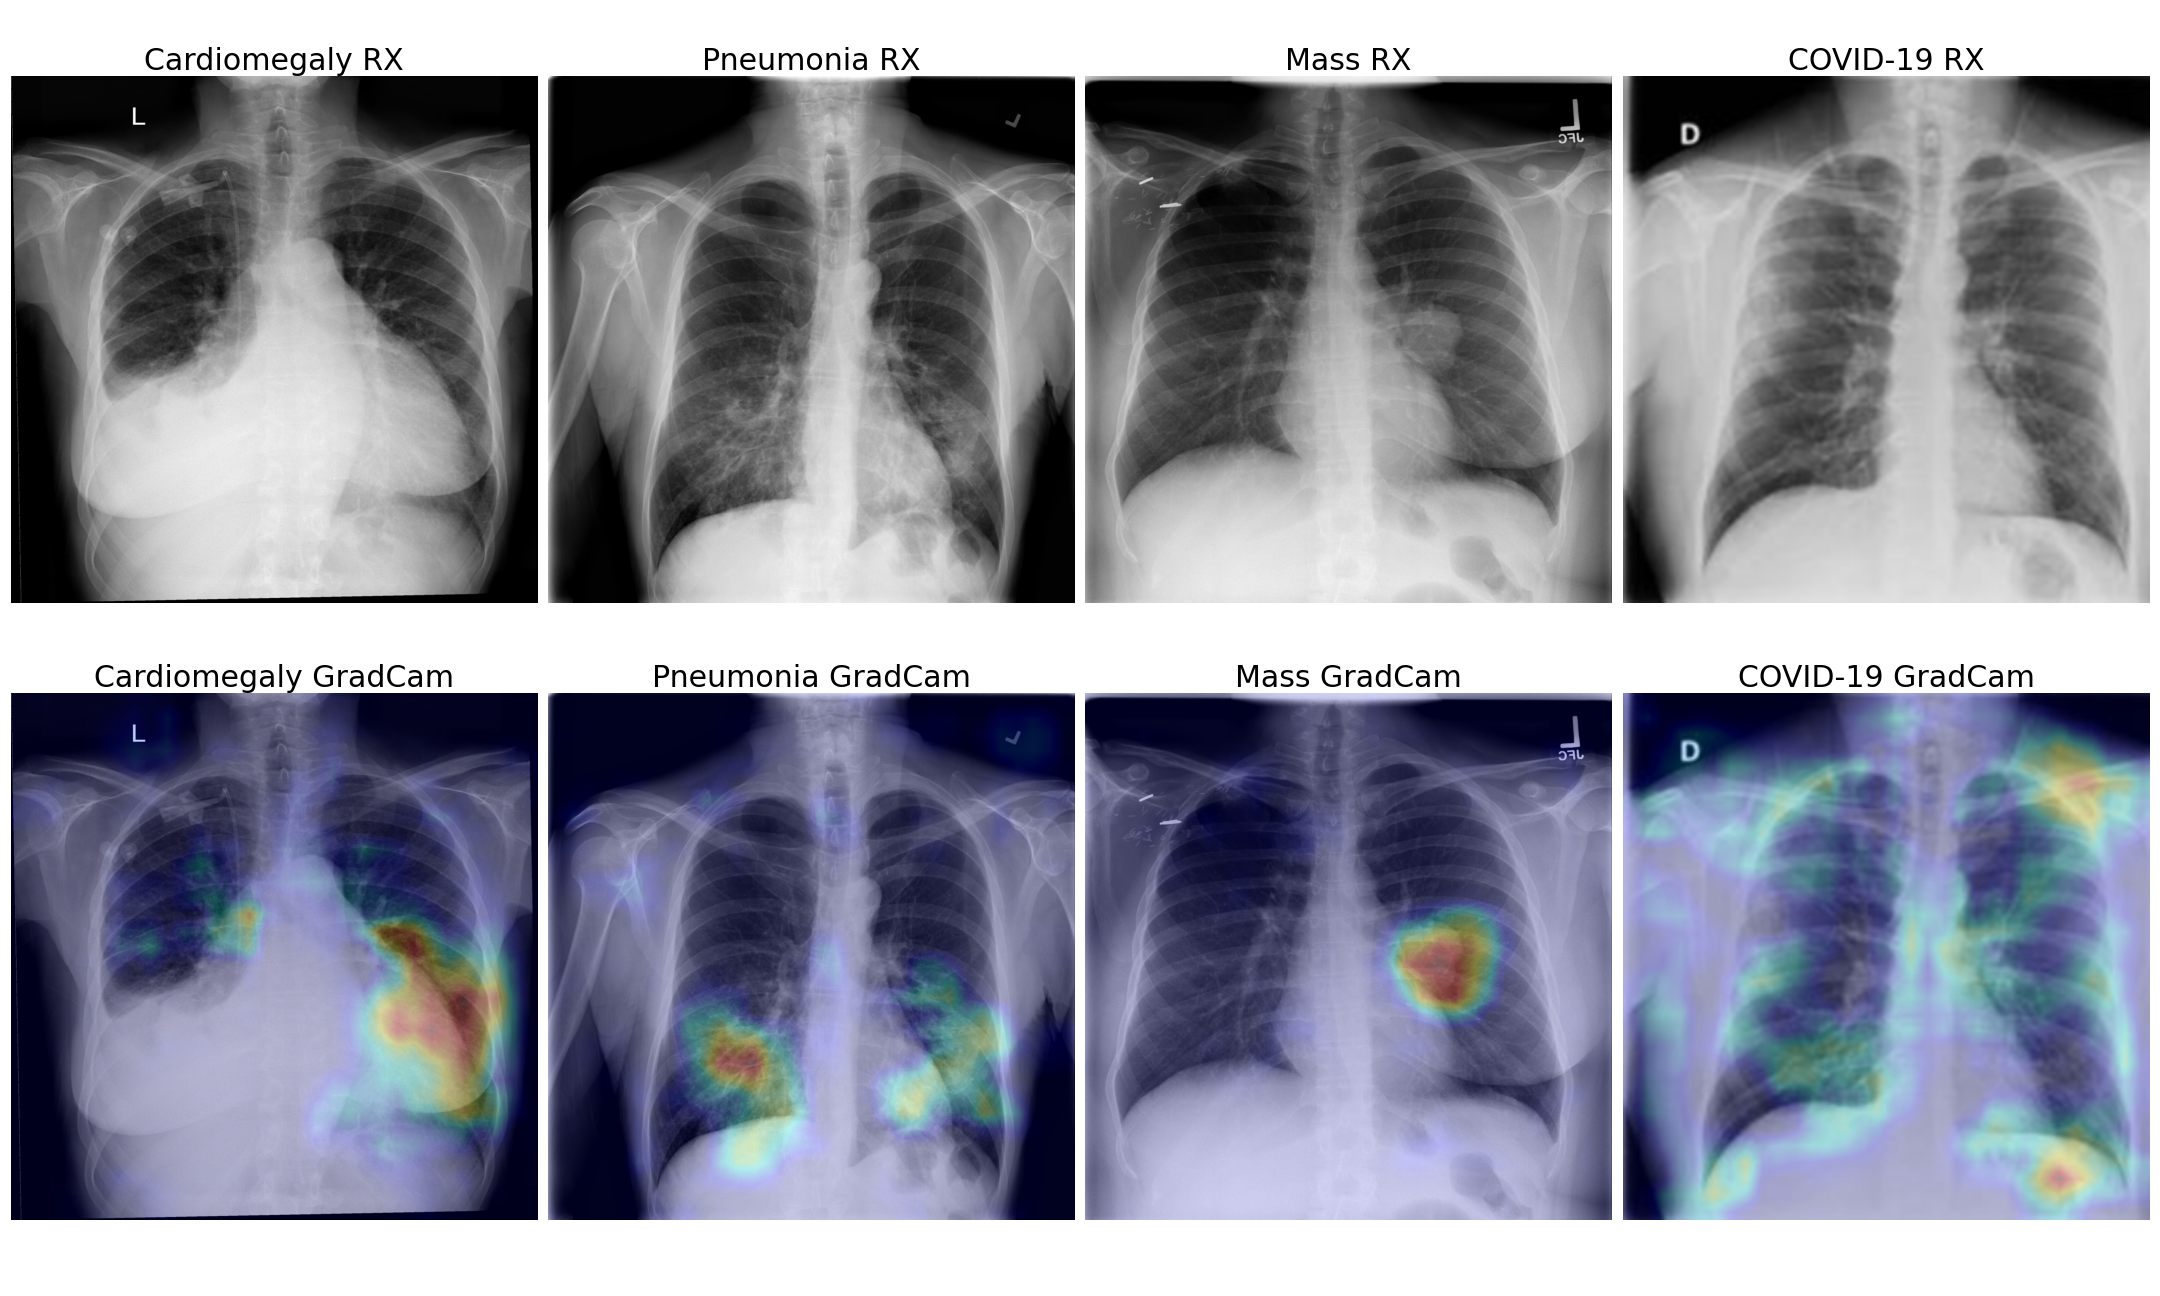
\includegraphics[width=0.8 \textwidth]{Chapters/4. ViT-Lung/images/vlgrid.png}
    \caption{Algunas imágenes de rayos-X (primer fila) con diferentes patologías y sus imágenes GradCam
             asociadas en la segunda fila. La primera columna muestra un corazón crecido, la segunda
             columna corresponde a neumonía, la tercer columna muestra una especie de tejido inusual
             en el pulmón y la última columna un caso de COVID-19.}
    \label{img-results}
\end{figure}

De manera general, el rendimiento del modelo convolucional basado en \textit{ResNet50} es mayor al
modelo de atención basado en \textit{ViT}. Cabe resaltar que solo existe una diferencia en ambos modelos
que podría mejorar los resultados en favor del modelo \textit{ViT}: la resolución de las imágenes. El
modelo \textit{ViT} trabaja con imágenes más pequeñas que el modelo \textit{ResNet50}, $384\times384$ y
$1024\times1024$ respectivamente. Dicha limitante se debe a la capacidad computacional requerida y con la
que se contó para el entrenamiento, ya que el modelo basado en \textit{ViT} requiere un consumo de memoria
mucho mayor para su procesamiento.


\begin{figure}[b]
    \centering
    \begin{subfigure}{0.4\textwidth}
        \centering
        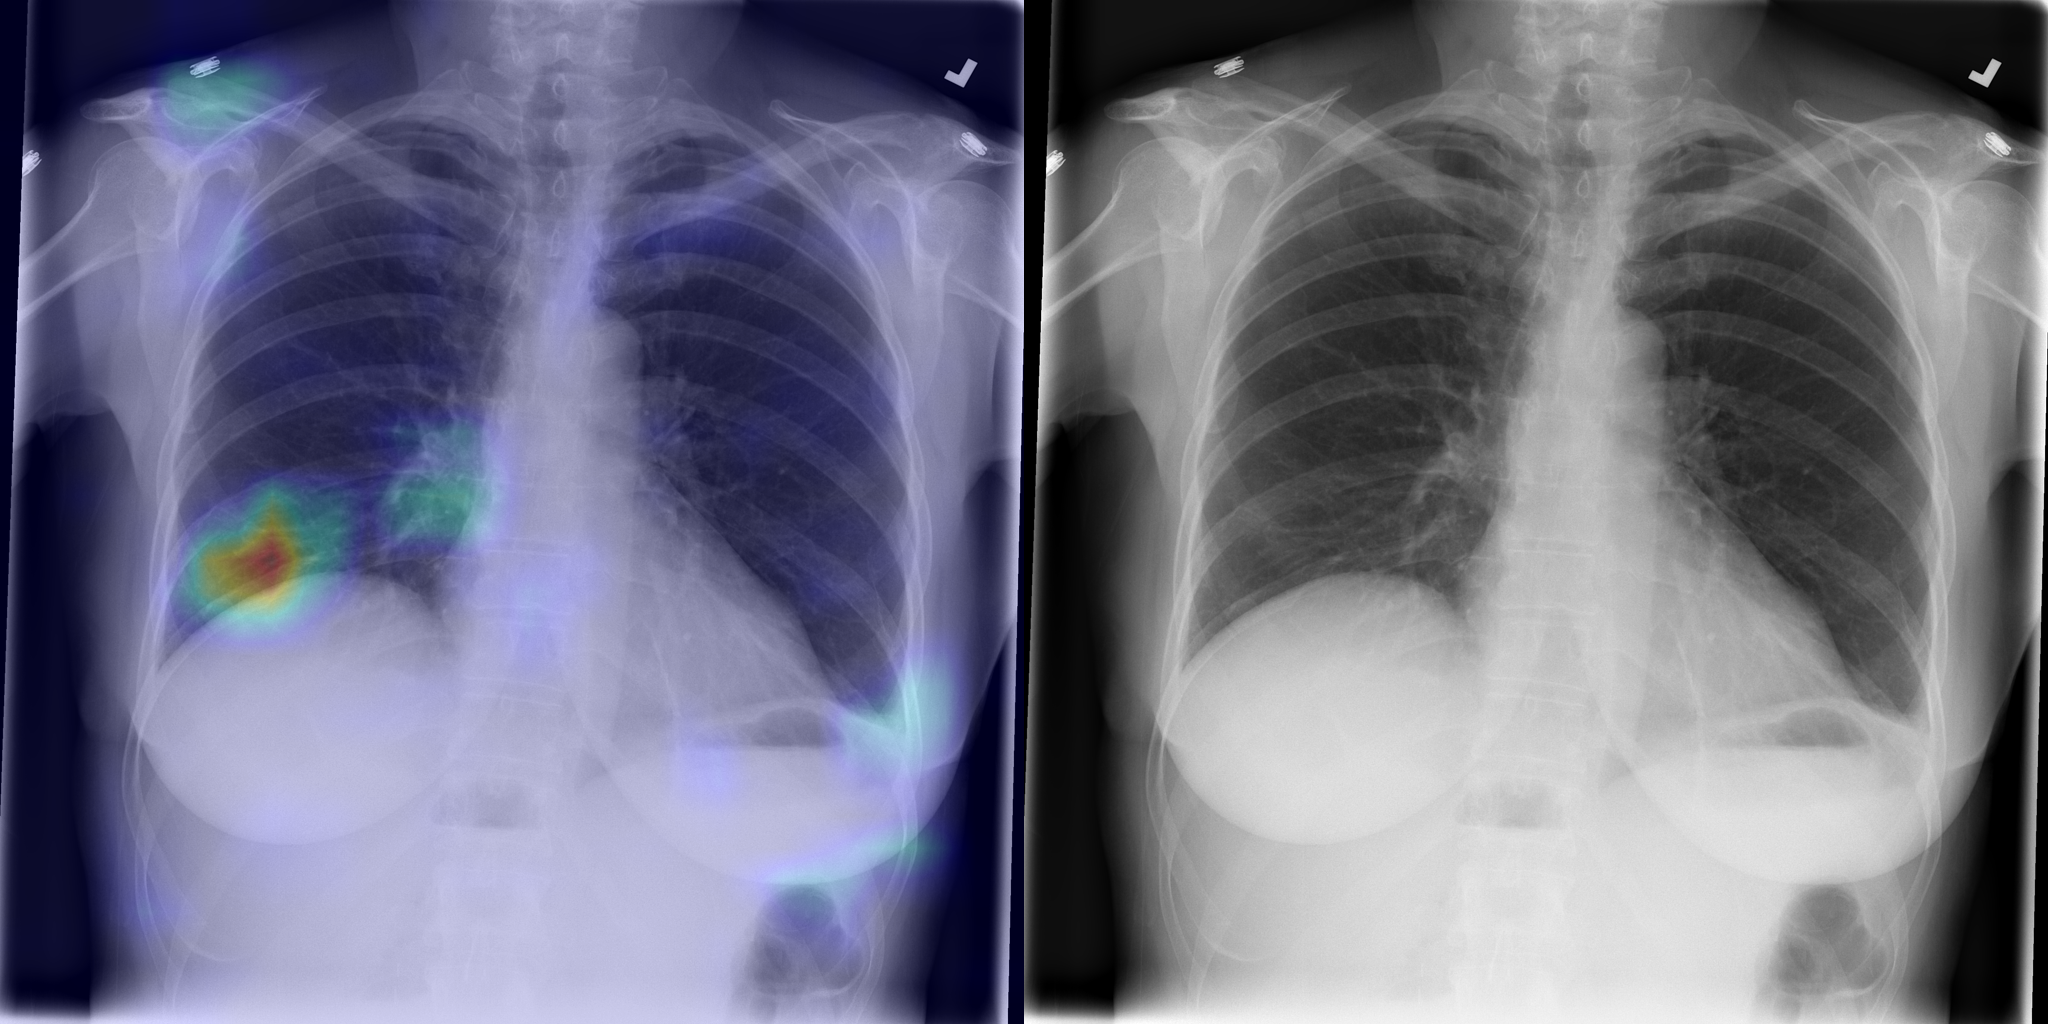
\includegraphics[width=1.0\textwidth]{Chapters/5. Conclusiones/img/Atelectasis/1_1_00000147_001.png}
    \end{subfigure}
    \begin{subfigure}{0.4\textwidth}
        \centering
        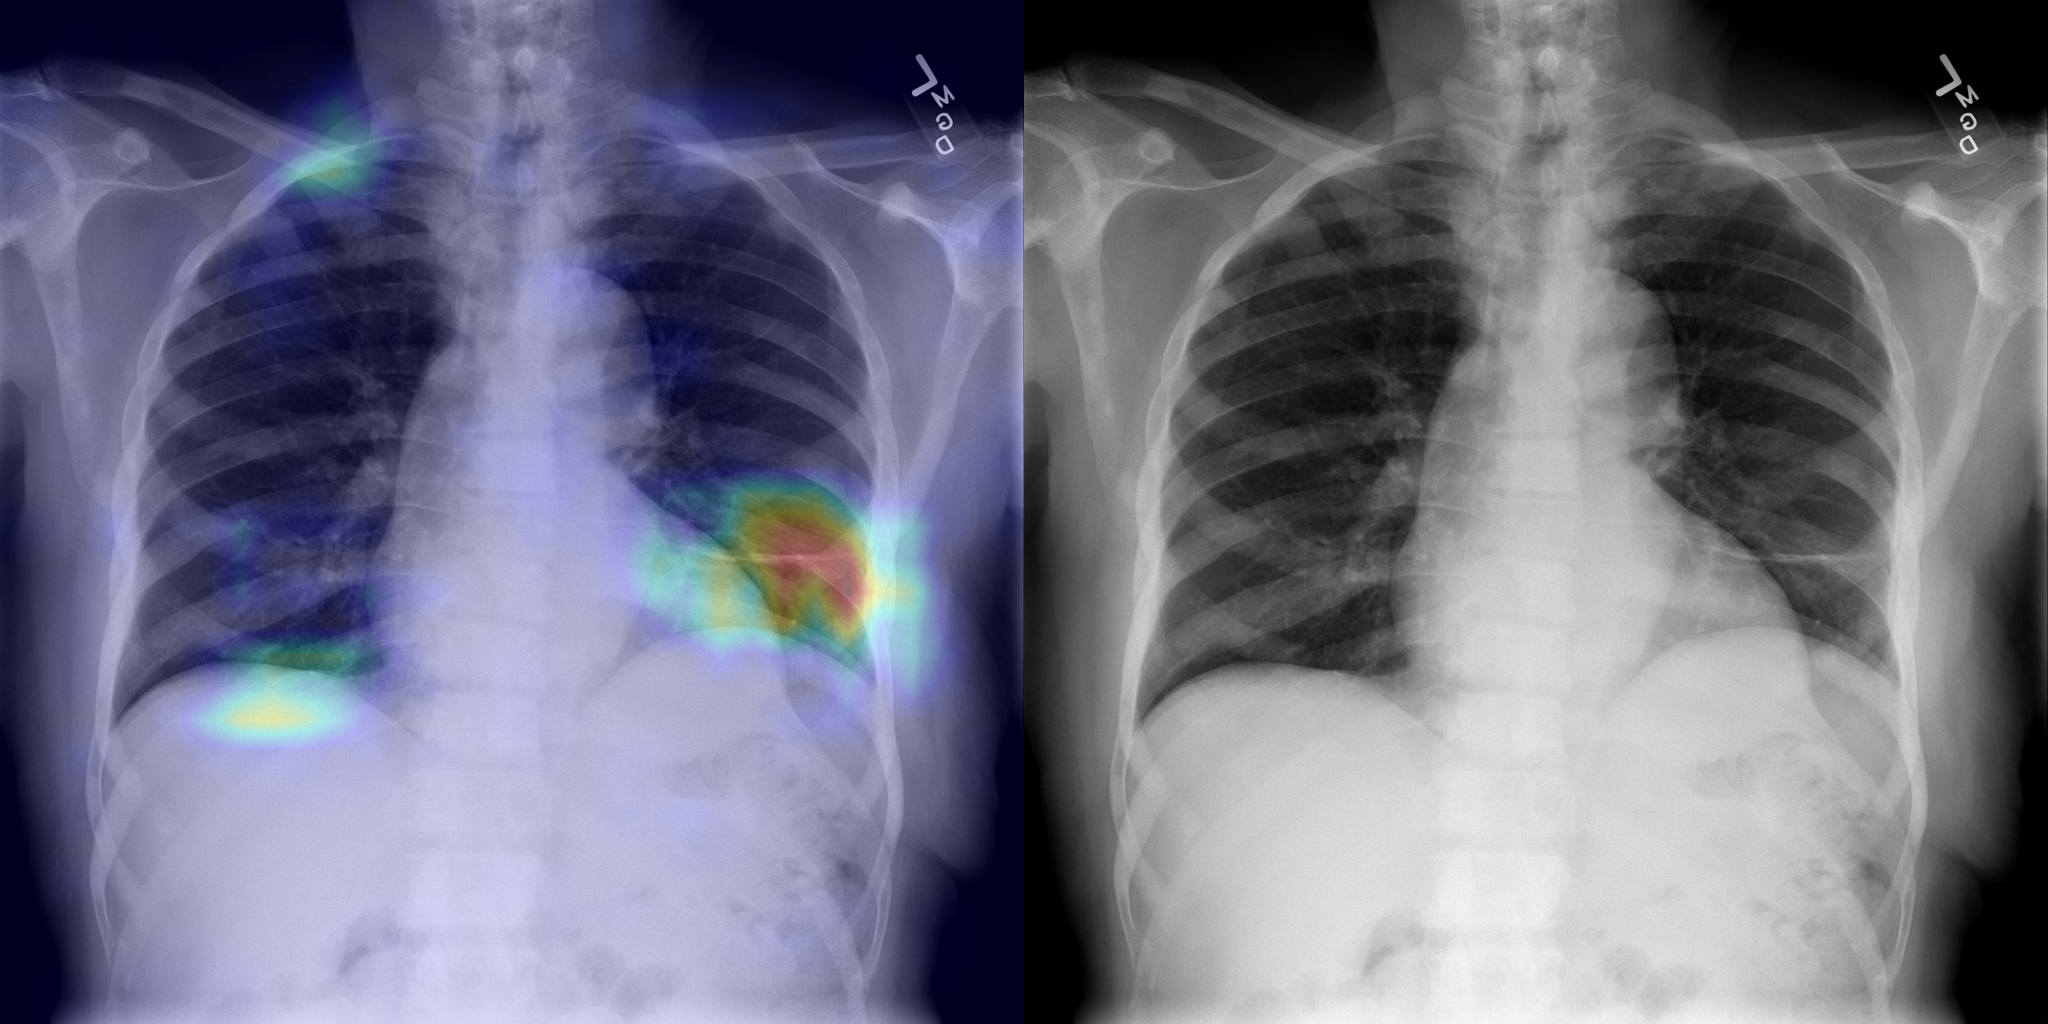
\includegraphics[width=1.0\textwidth]{Chapters/5. Conclusiones/img/Atelectasis/1_1_00000149_002.png}
    \end{subfigure}
    \begin{subfigure}{0.4\textwidth}
        \centering
        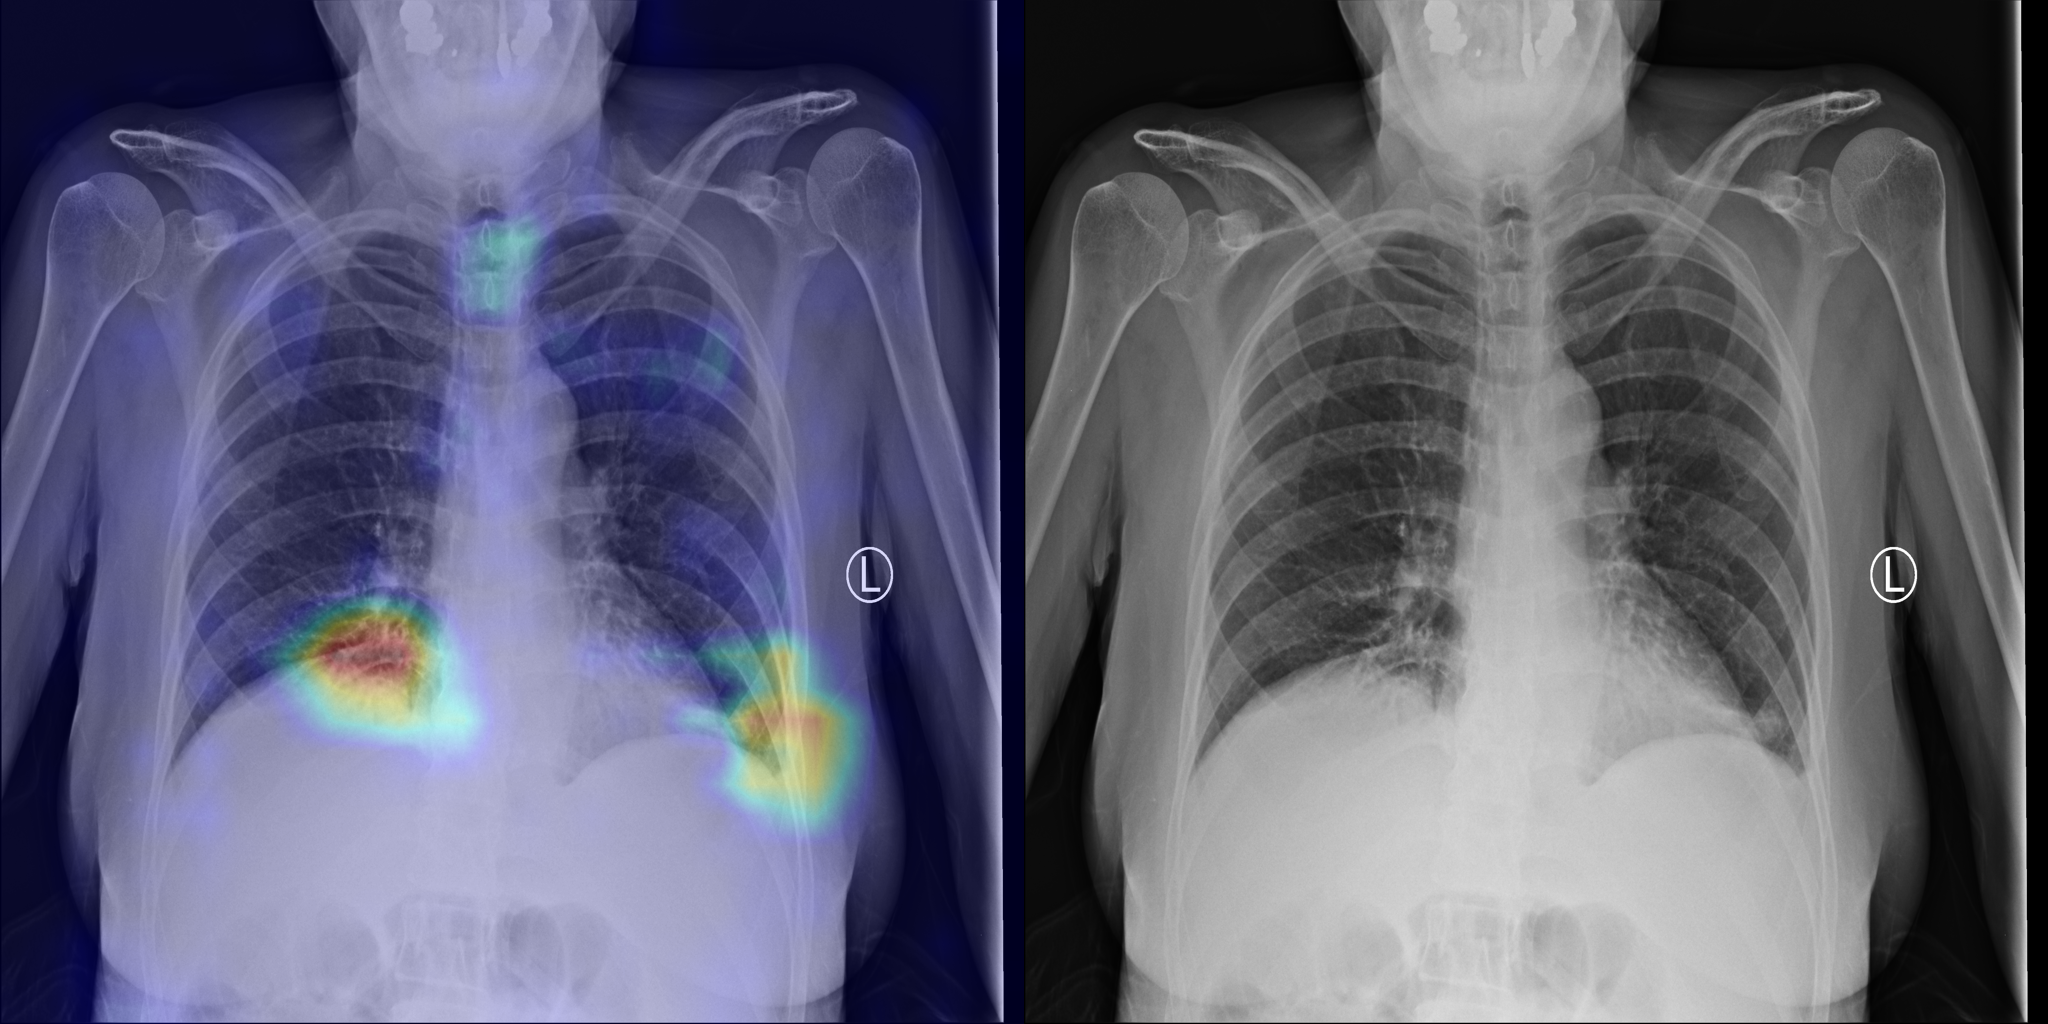
\includegraphics[width=1.0\textwidth]{Chapters/5. Conclusiones/img/Atelectasis/1_1_00000150_003.png}
    \end{subfigure}
    \begin{subfigure}{0.4\textwidth}
        \centering
        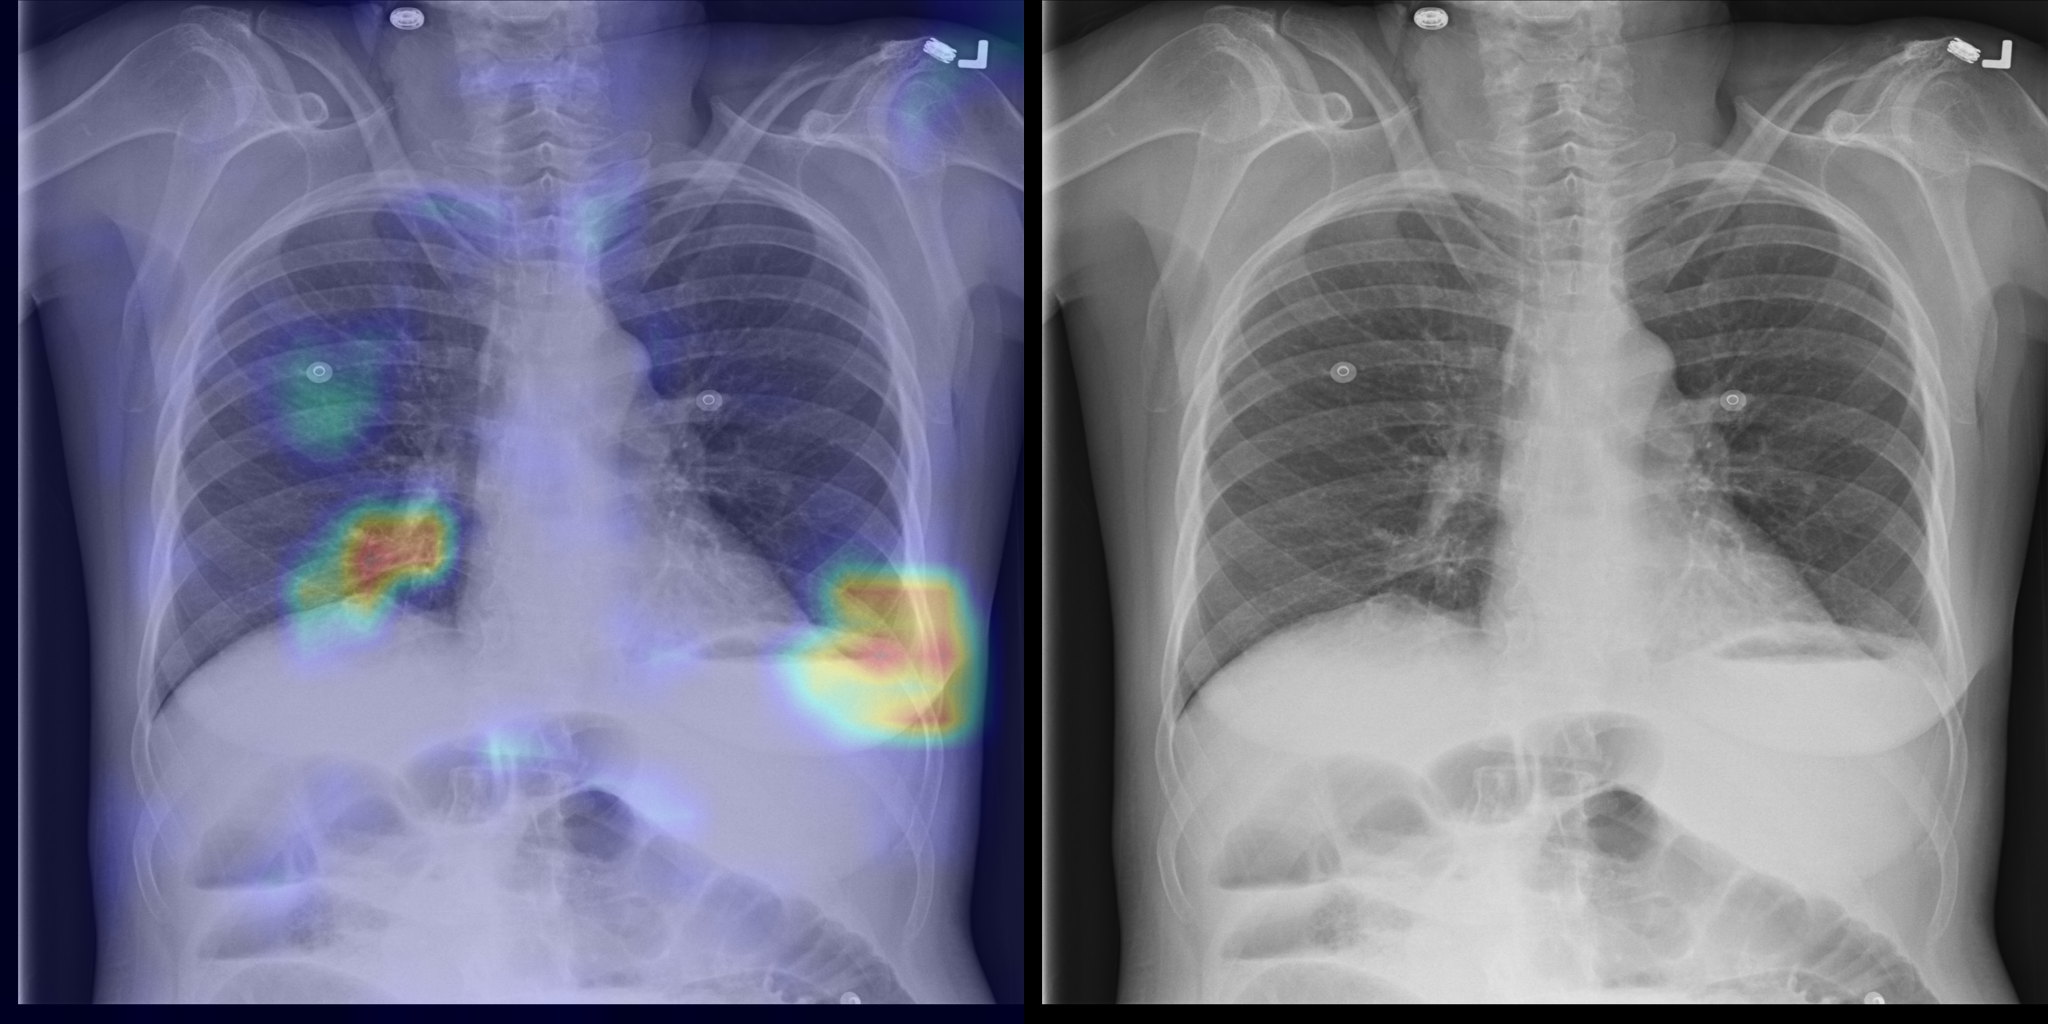
\includegraphics[width=1.0\textwidth]{Chapters/5. Conclusiones/img/Atelectasis/1_1_00000150_004.png}
    \end{subfigure}
    \begin{subfigure}{0.4\textwidth}
        \centering
        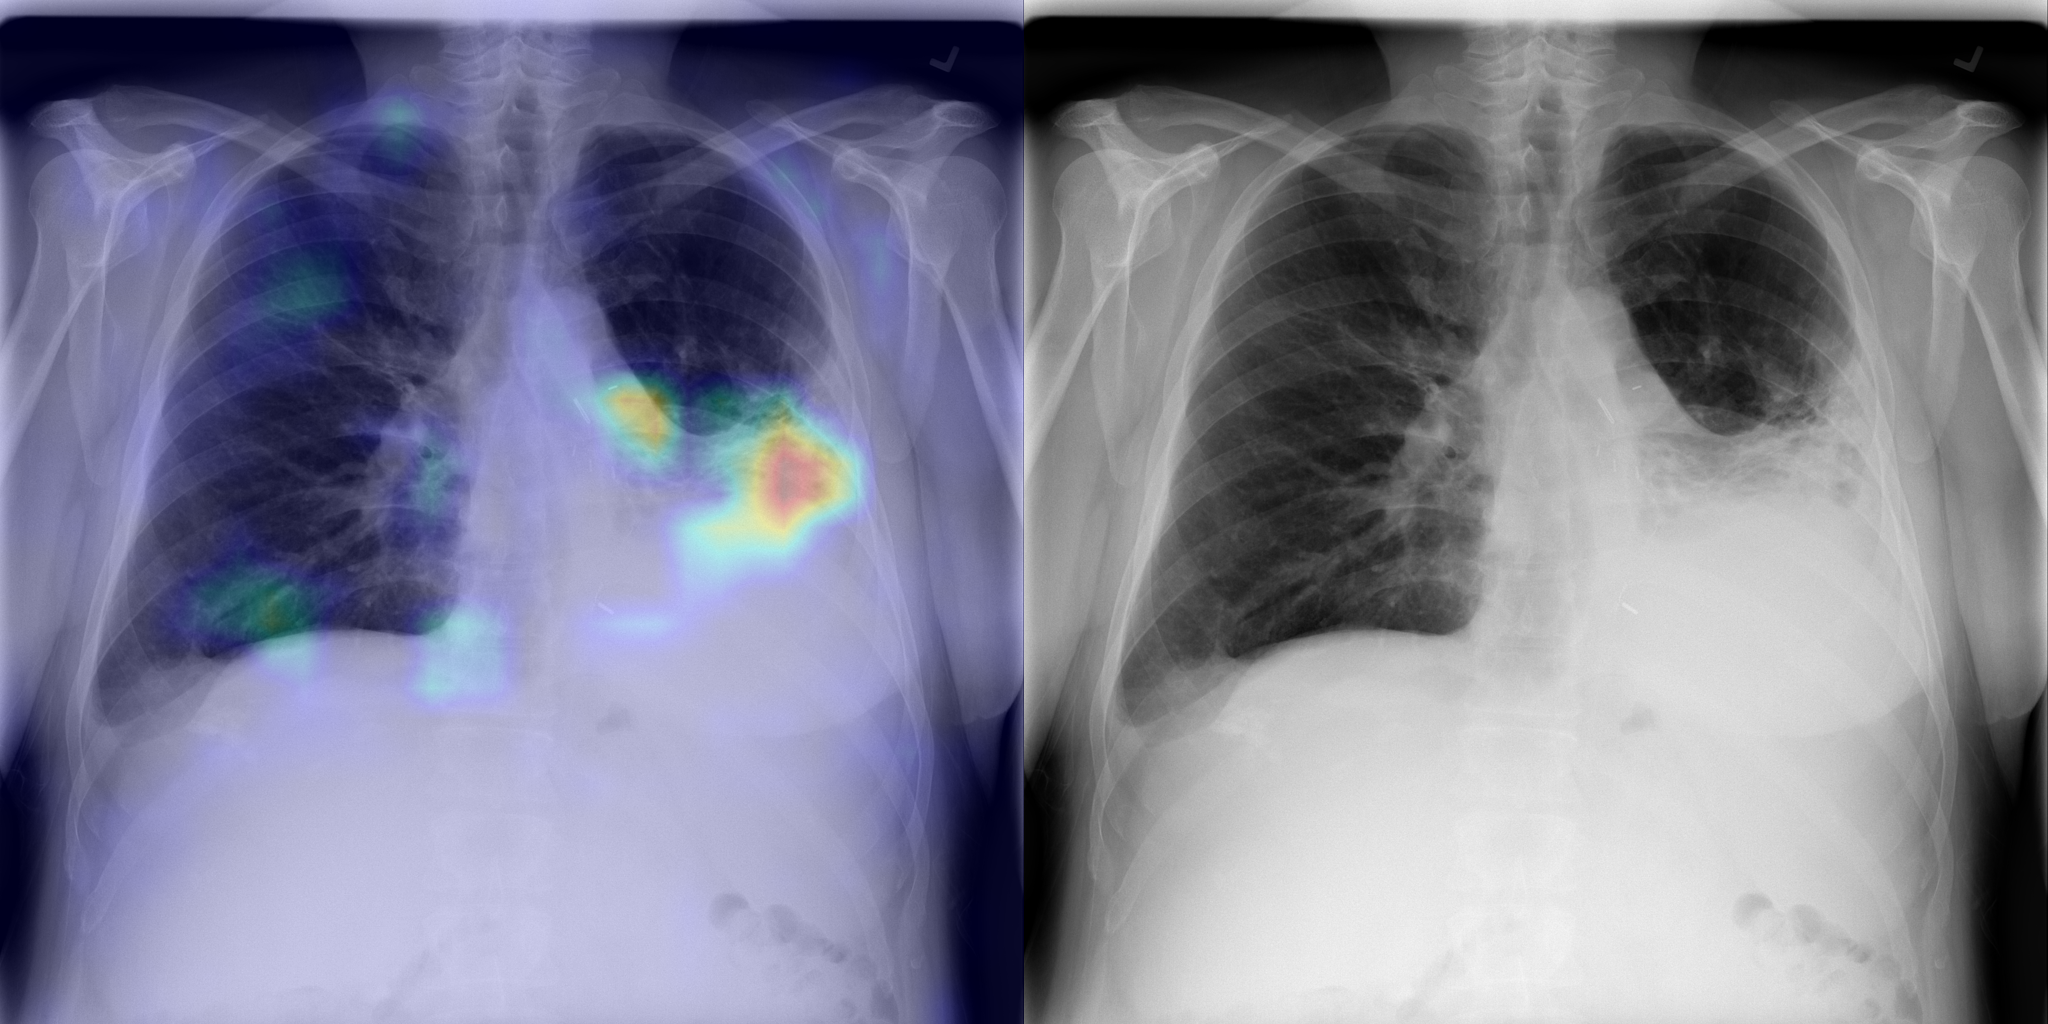
\includegraphics[width=1.0\textwidth]{Chapters/5. Conclusiones/img/Atelectasis/1_1_00000467_000.png}
    \end{subfigure}
    \begin{subfigure}{0.4\textwidth}
        \centering
        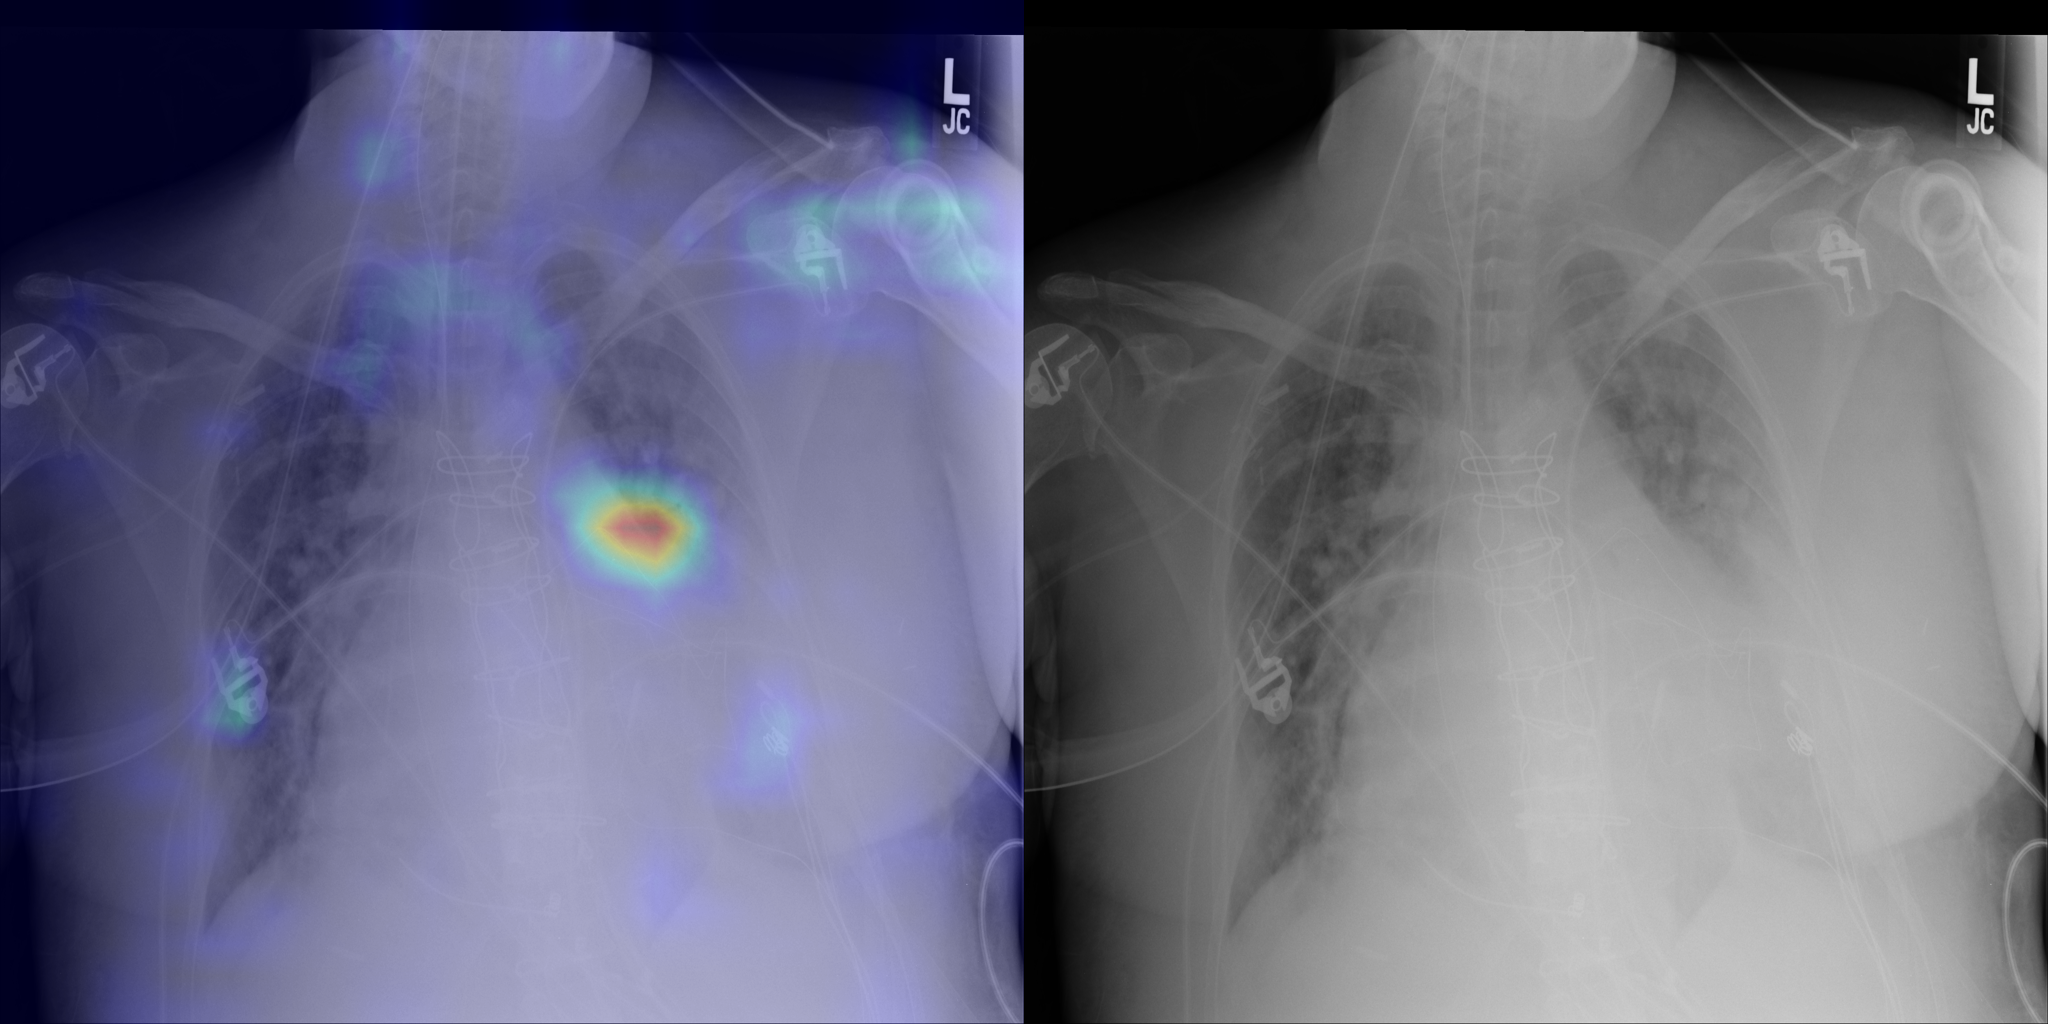
\includegraphics[width=1.0\textwidth]{Chapters/5. Conclusiones/img/Atelectasis/1_1_00000032_036.png}
    \end{subfigure}
    \begin{subfigure}{0.4\textwidth}
        \centering
        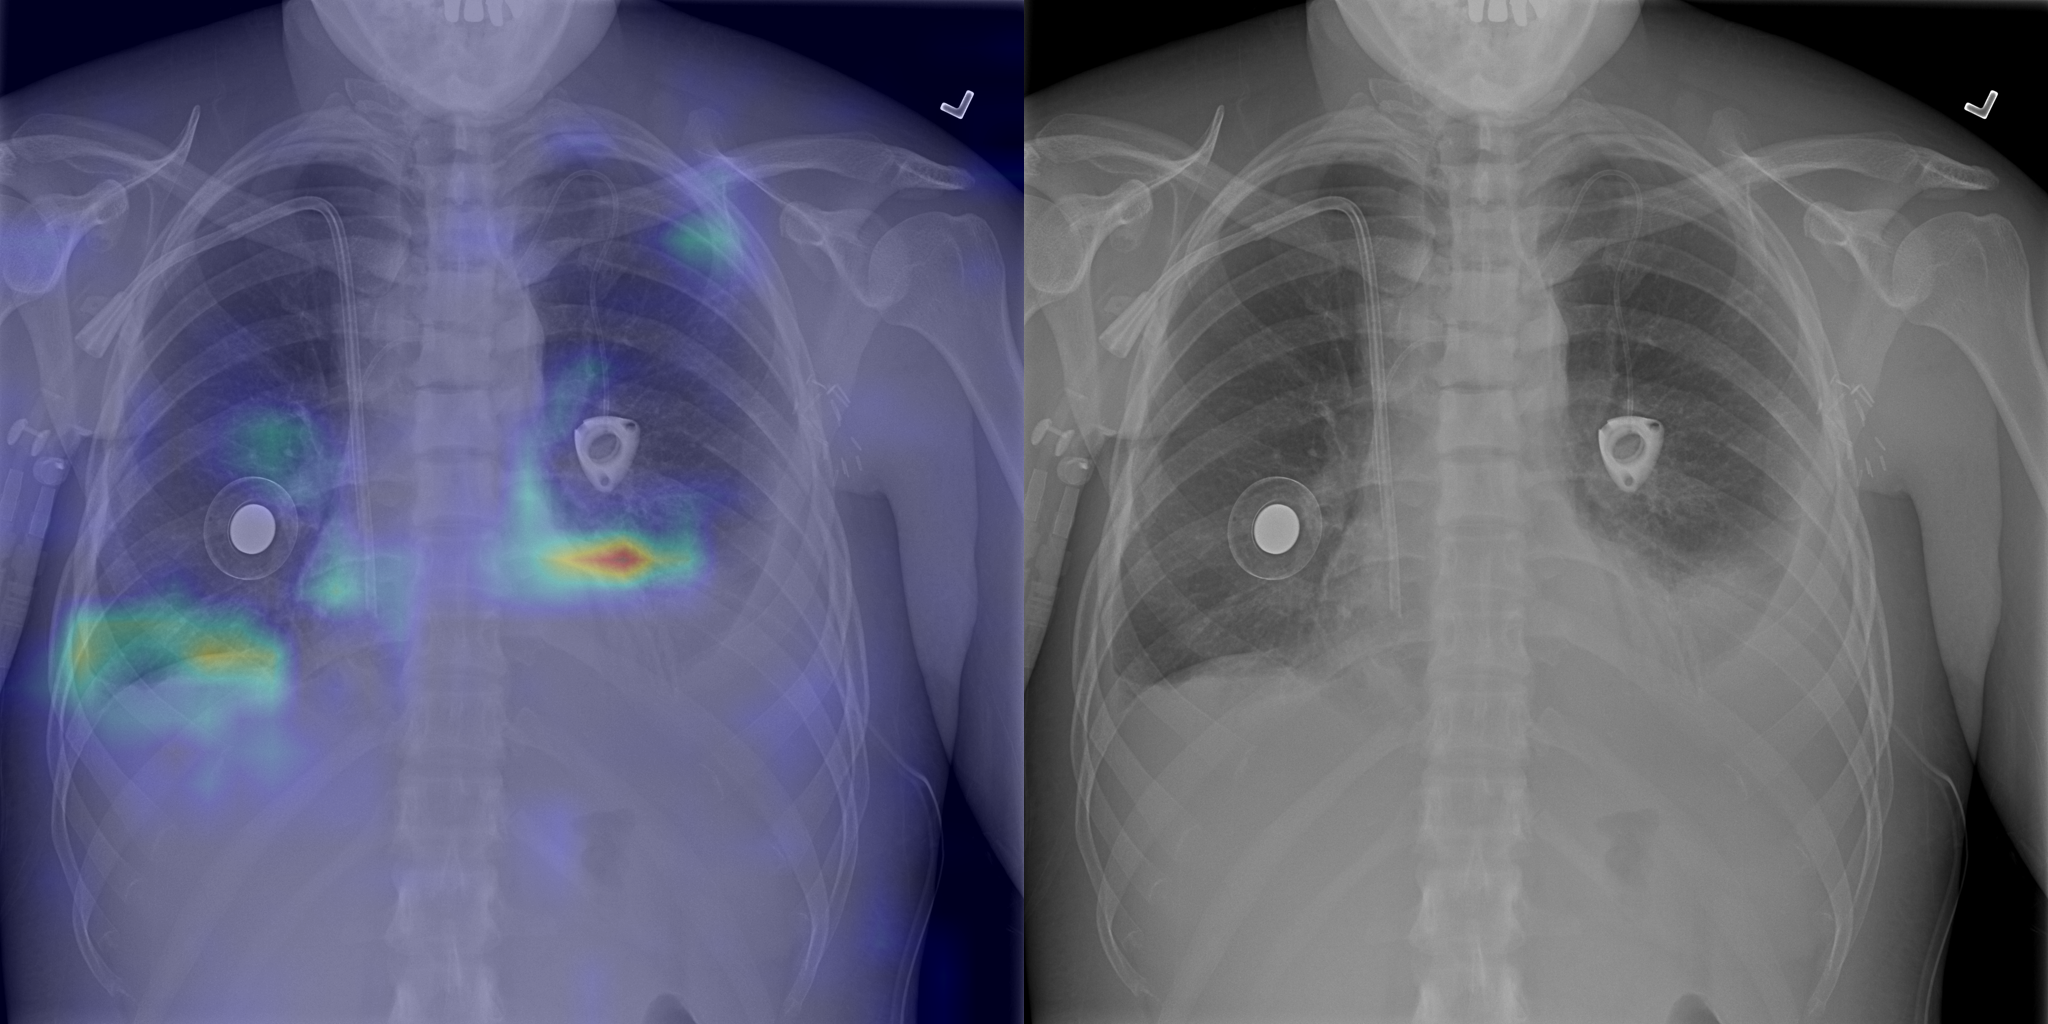
\includegraphics[width=1.0\textwidth]{Chapters/5. Conclusiones/img/Atelectasis/1_1_00029596_022.png}
    \end{subfigure}
    \begin{subfigure}{0.4\textwidth}
        \centering
        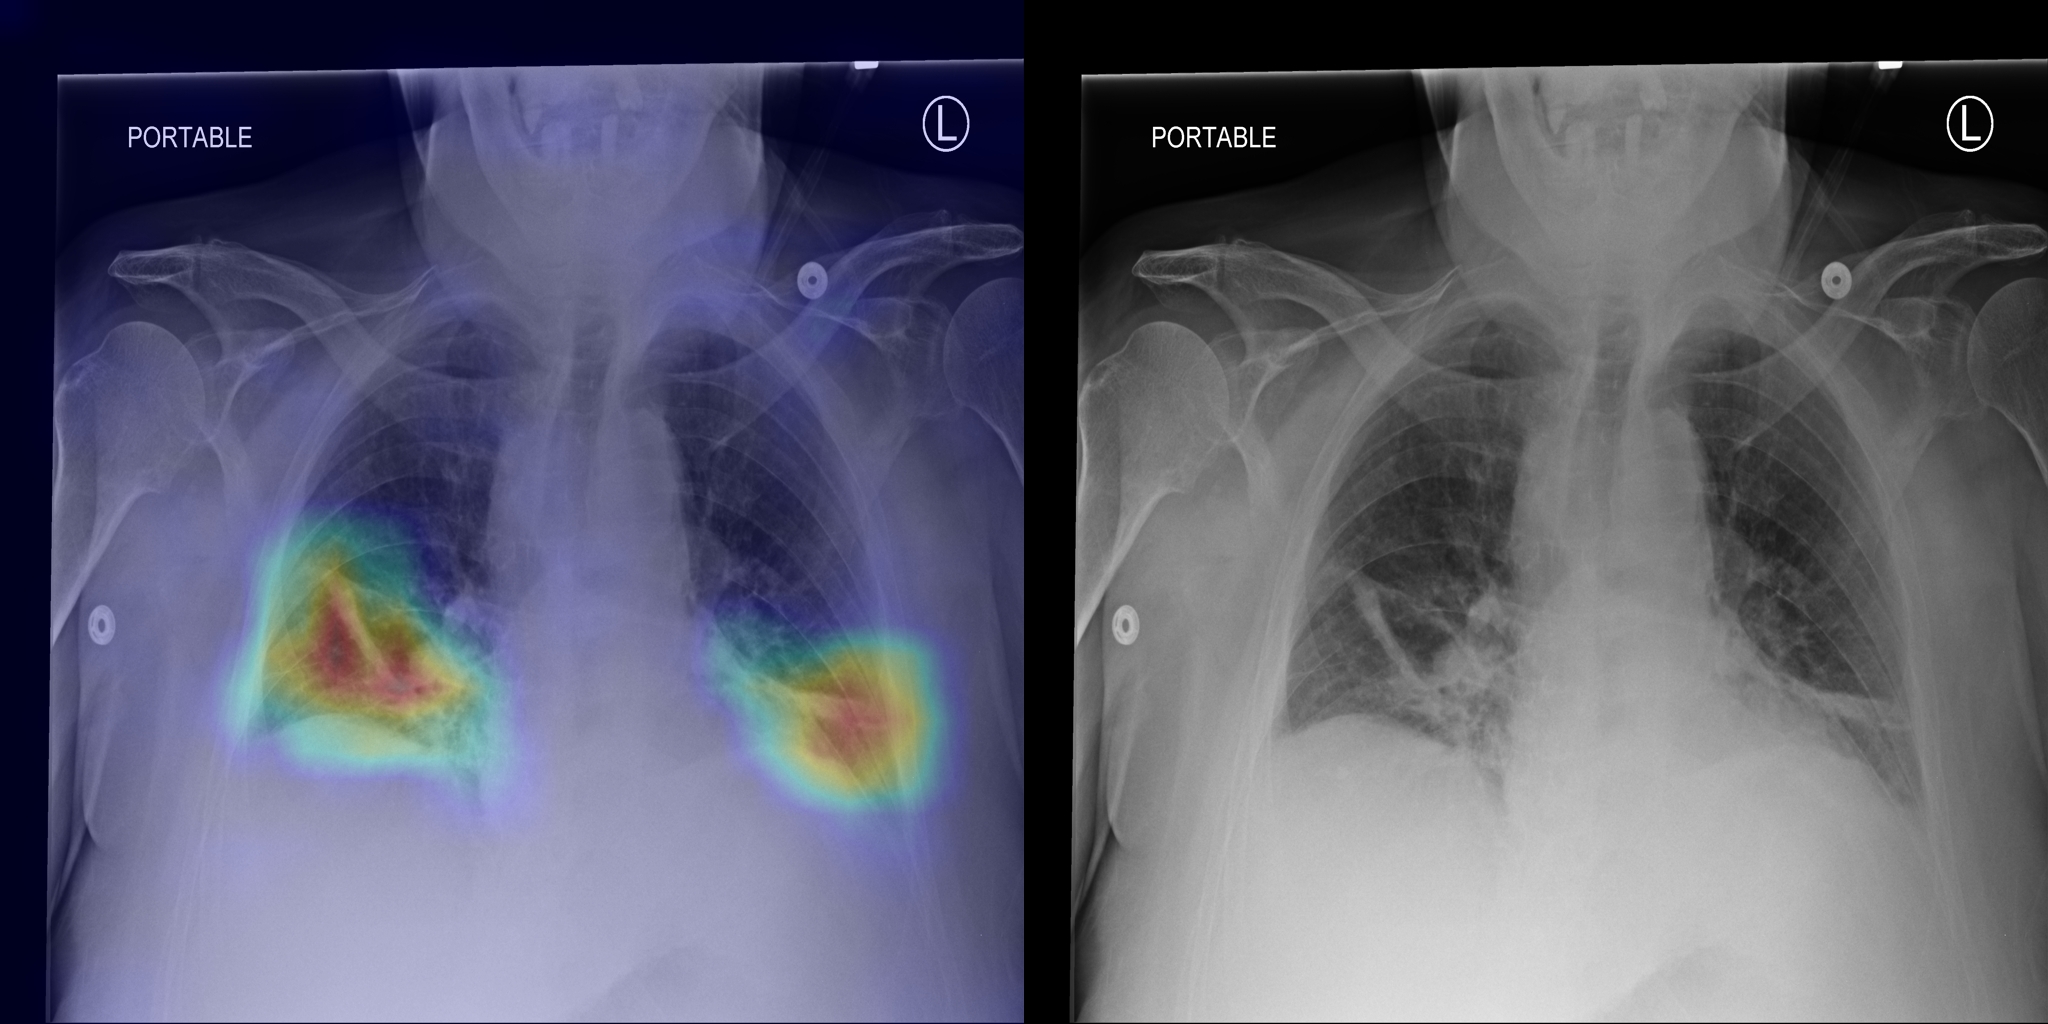
\includegraphics[width=1.0\textwidth]{Chapters/5. Conclusiones/img/Atelectasis/1_1_00030408_000.png}
    \end{subfigure}
    \begin{subfigure}{0.4\textwidth}
        \centering
        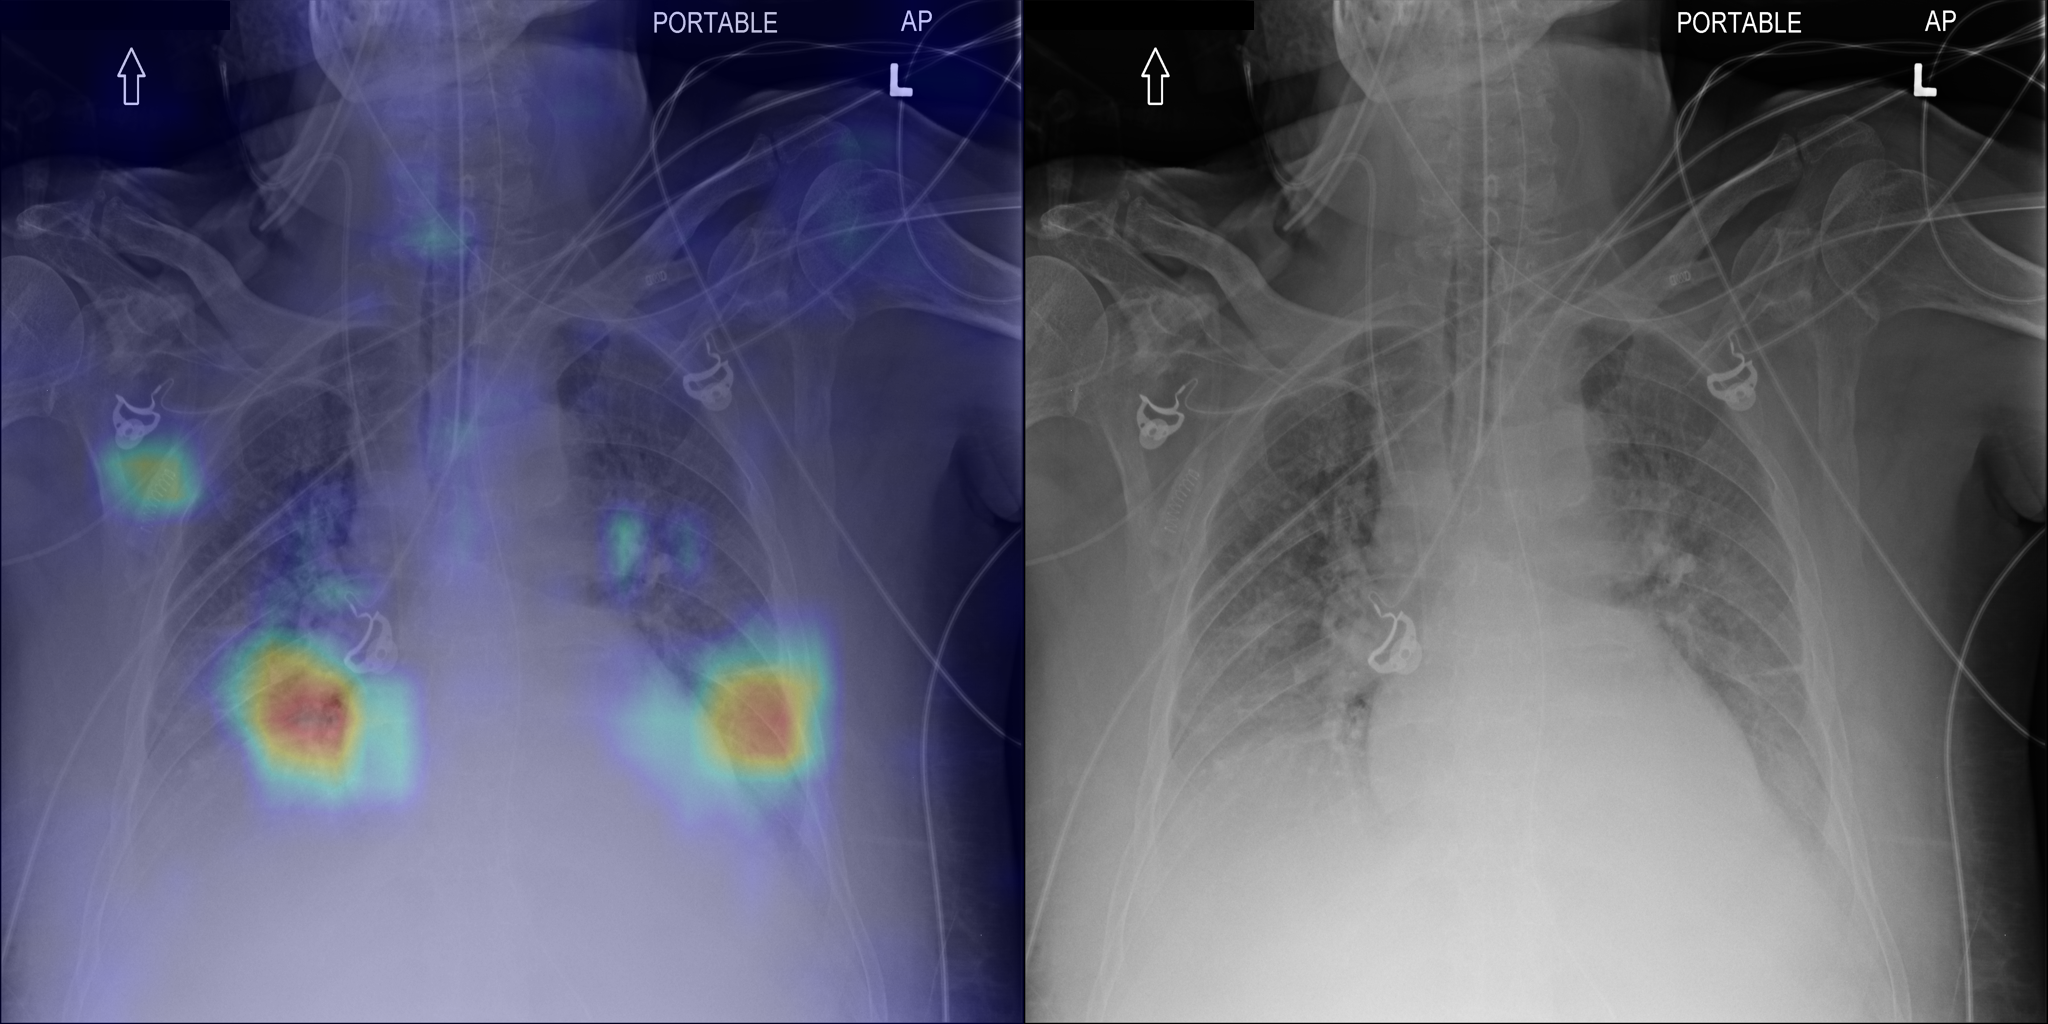
\includegraphics[width=1.0\textwidth]{Chapters/5. Conclusiones/img/Atelectasis/1_1_00030408_013.png}
    \end{subfigure}
    \begin{subfigure}{0.4\textwidth}
        \centering
        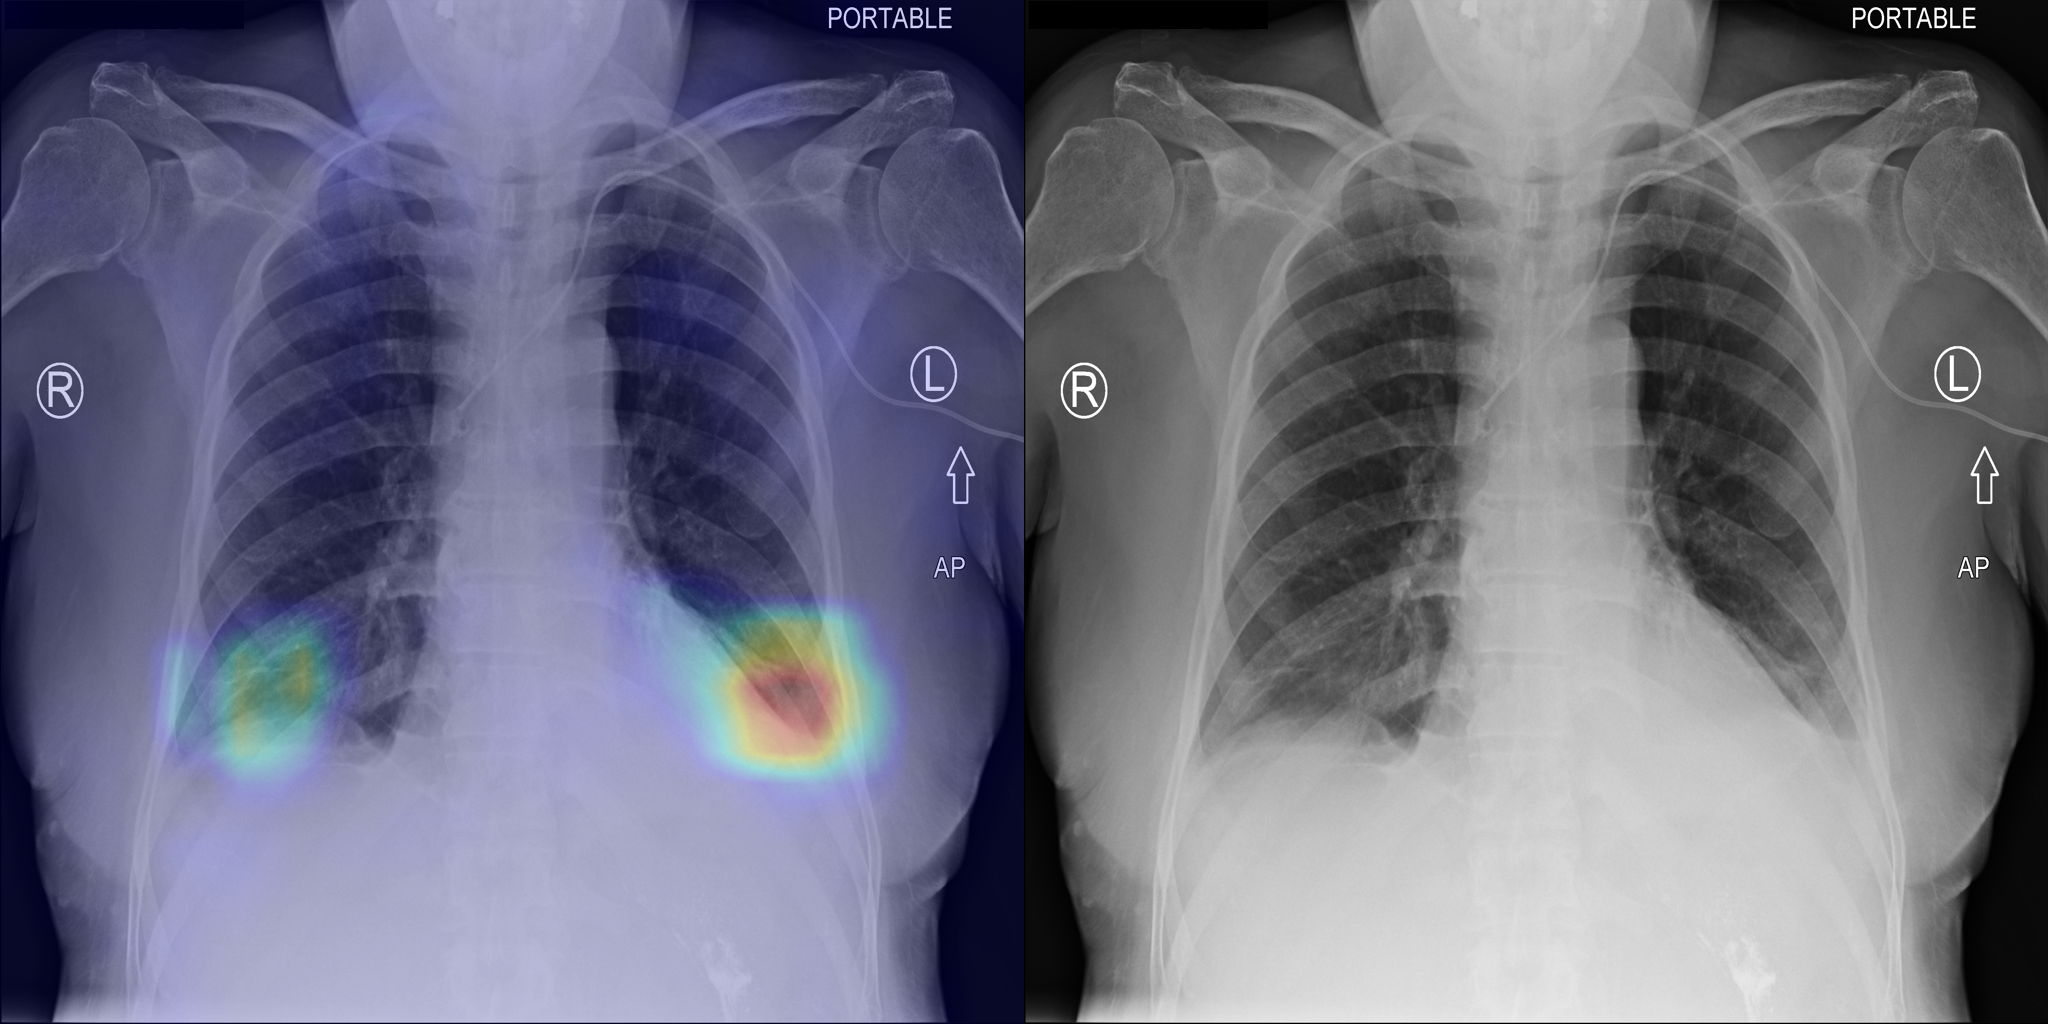
\includegraphics[width=1.0\textwidth]{Chapters/5. Conclusiones/img/Atelectasis/1_1_00028974_018.png}
    \end{subfigure}

    \caption{Atelectasis. Radiografías detectadas con la patología de atelectasis por los
                    radiólogos. A la izquierda de cada imagen el GradCam correspondiente a la detección
                    de la patología como positivo por el modelo CNN.}
    \label{fig-atelectasis}
\end{figure}

\begin{figure}[b]
    \centering
    \begin{subfigure}{0.4\textwidth}
        \centering
        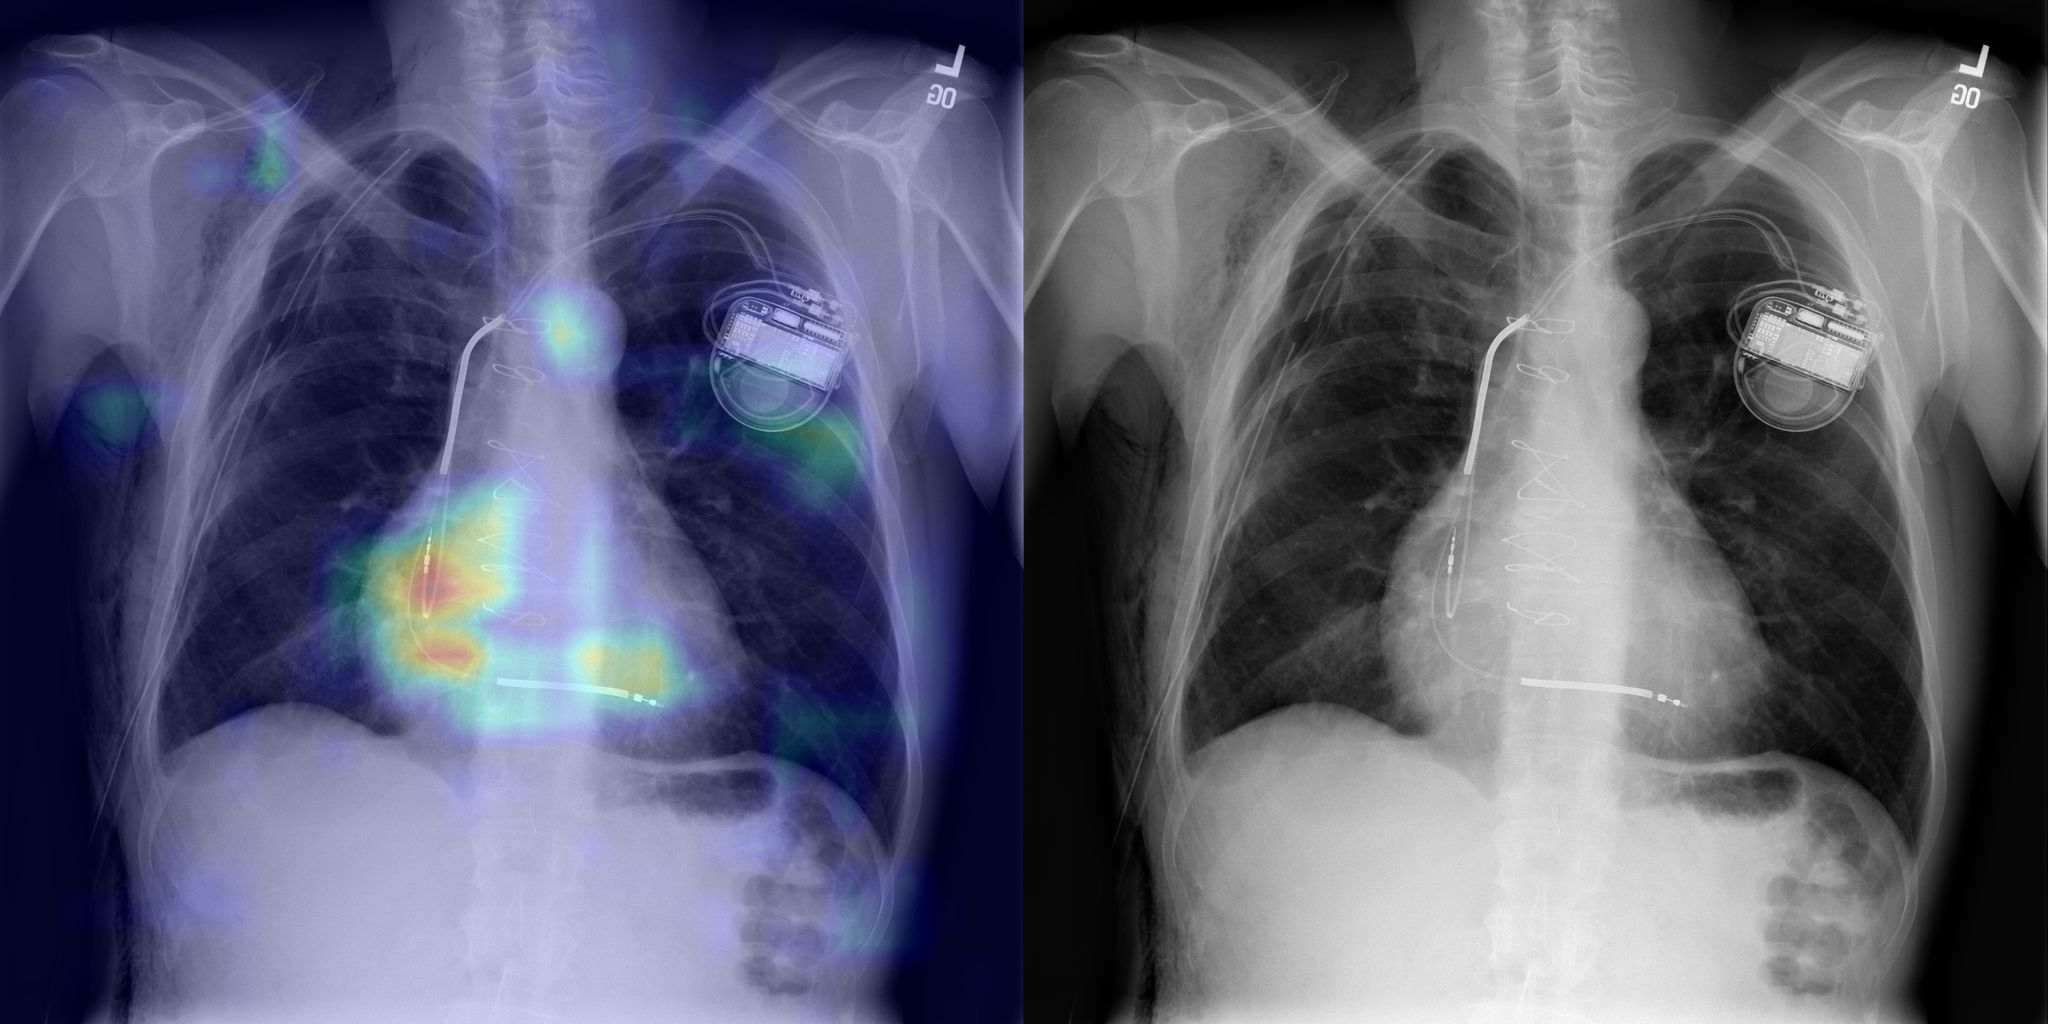
\includegraphics[width=1.0\textwidth]{Chapters/5. Conclusiones/img/Cardiomegaly/1_0_00000013_037.png}
    \end{subfigure}
    \begin{subfigure}{0.4\textwidth}
        \centering
        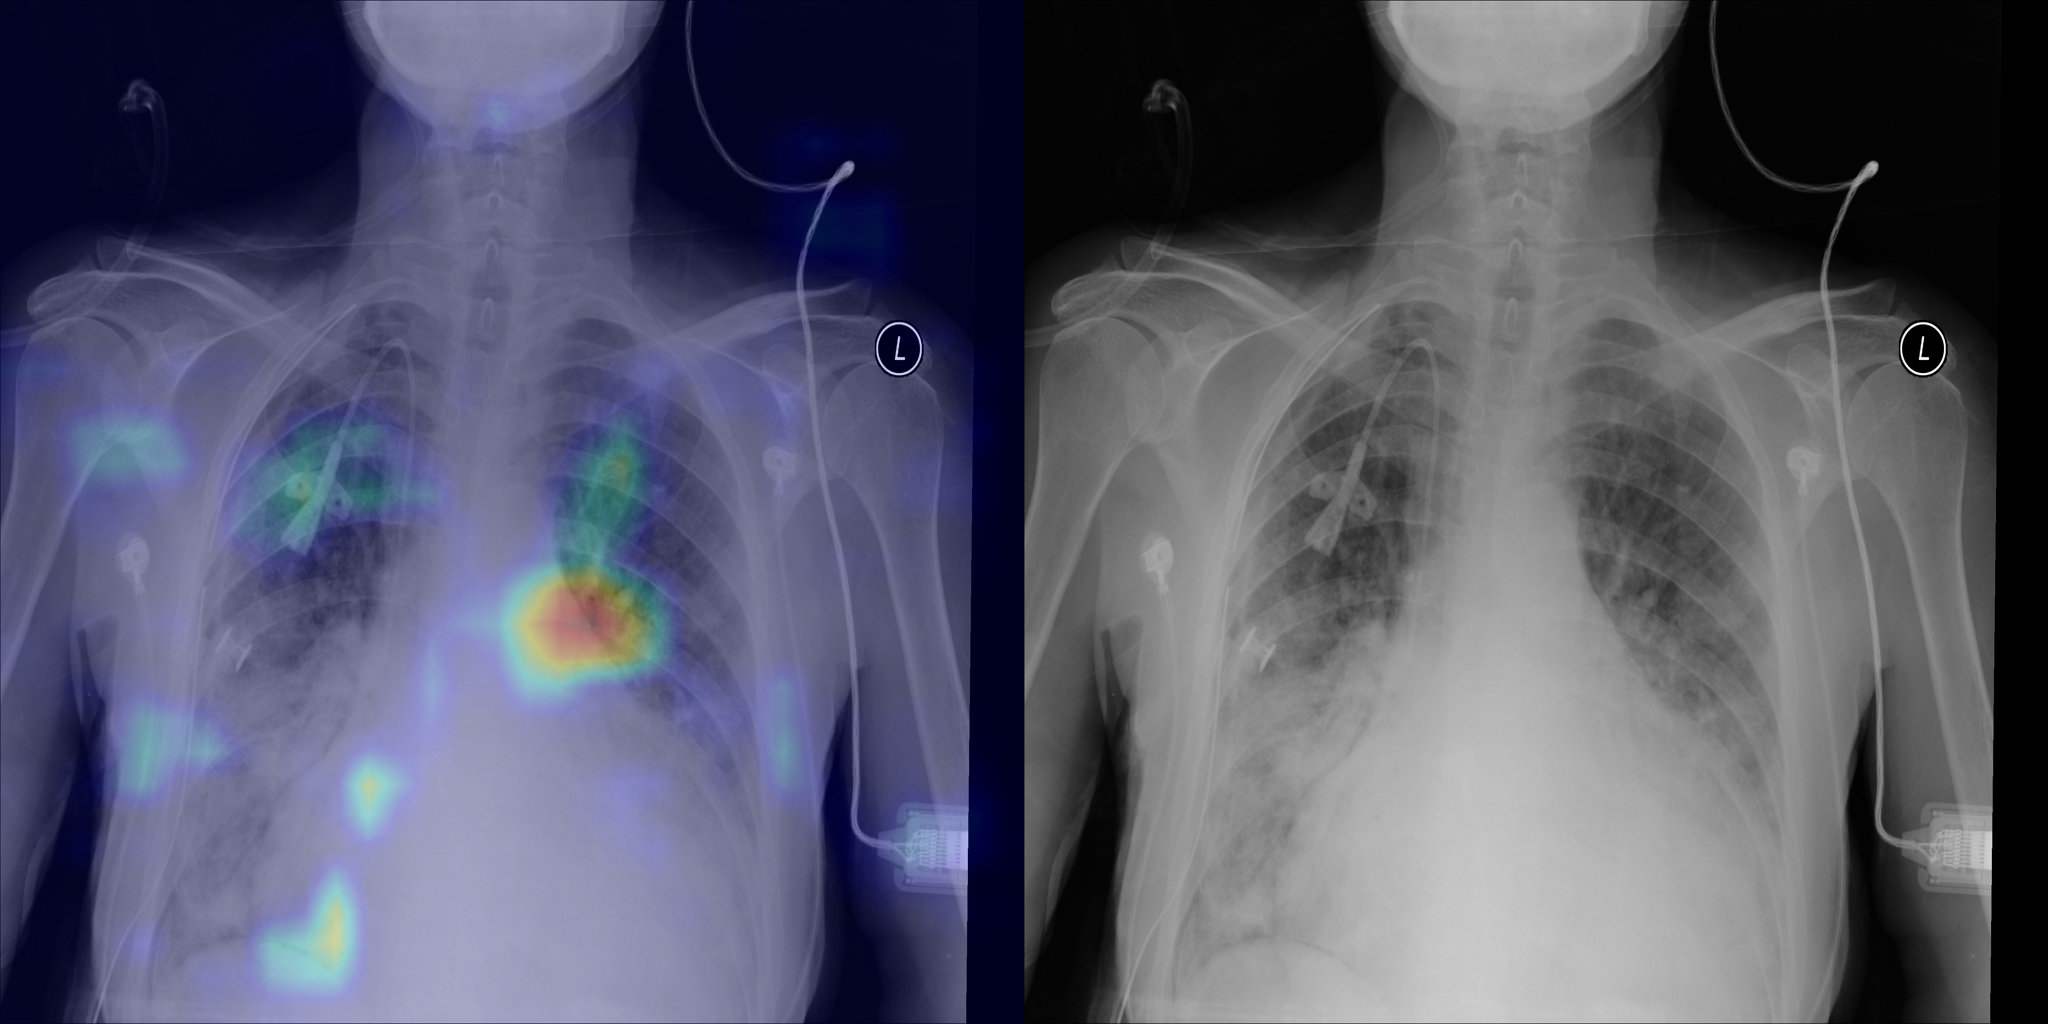
\includegraphics[width=1.0\textwidth]{Chapters/5. Conclusiones/img/Cardiomegaly/1_0_00000211_018.png}
    \end{subfigure}
    \begin{subfigure}{0.4\textwidth}
        \centering
        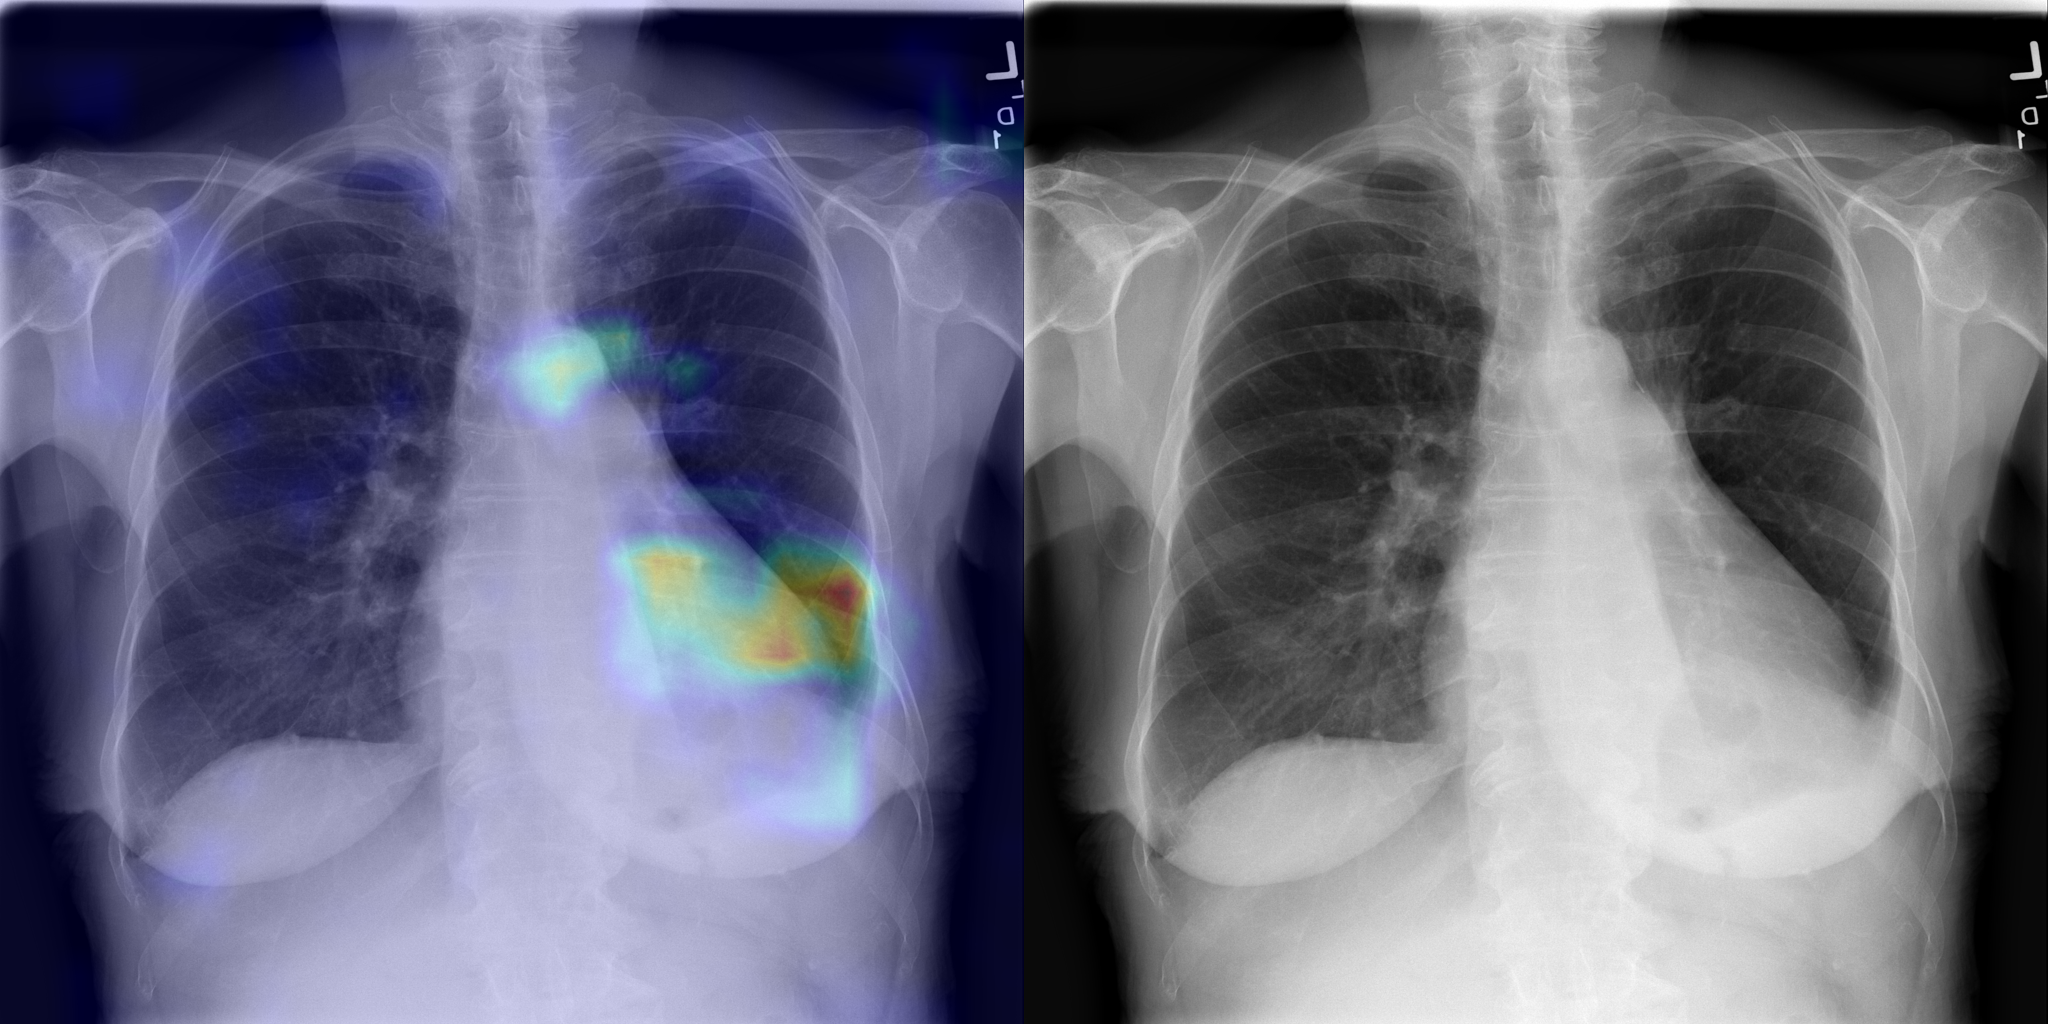
\includegraphics[width=1.0\textwidth]{Chapters/5. Conclusiones/img/Cardiomegaly/1_0_00000732_008.png}
    \end{subfigure}
    \begin{subfigure}{0.4\textwidth}
        \centering
        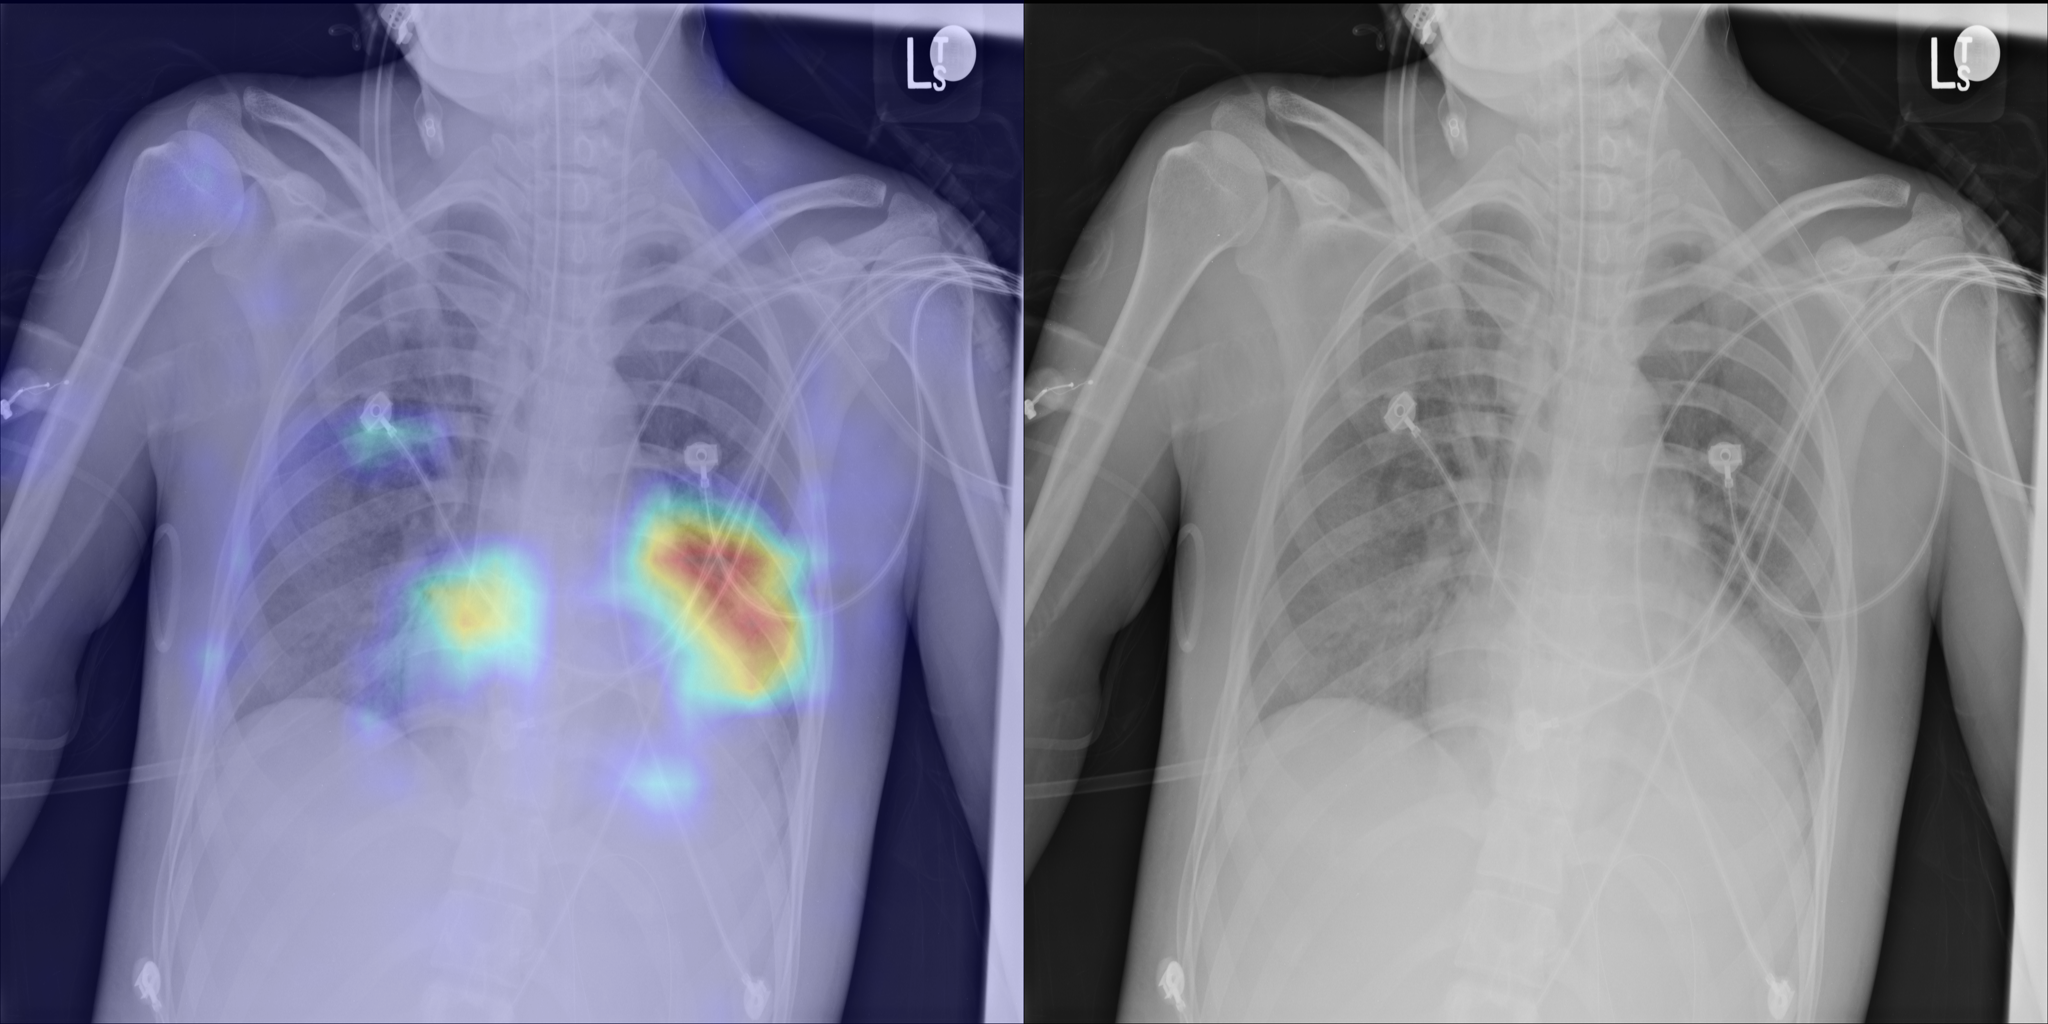
\includegraphics[width=1.0\textwidth]{Chapters/5. Conclusiones/img/Cardiomegaly/1_0_00001582_008.png}
    \end{subfigure}
    \begin{subfigure}{0.4\textwidth}
        \centering
        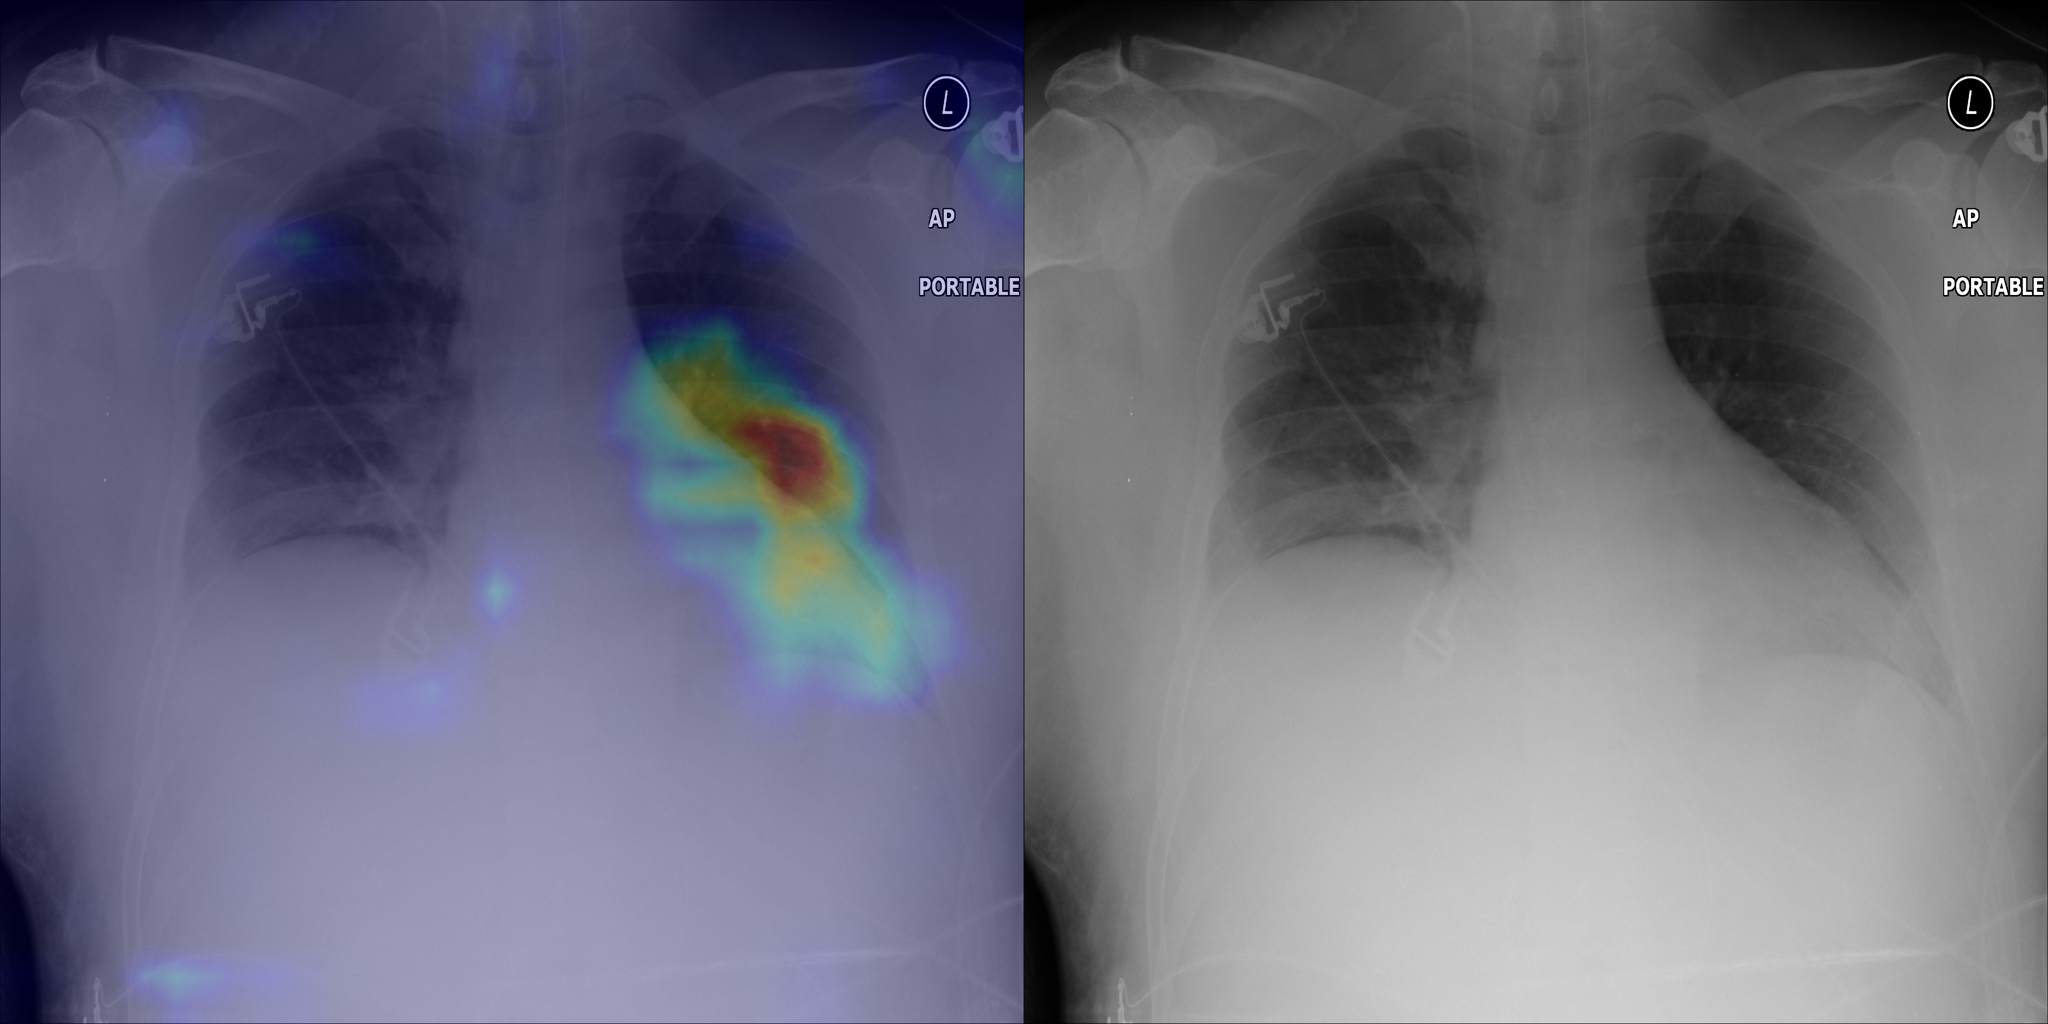
\includegraphics[width=1.0\textwidth]{Chapters/5. Conclusiones/img/Cardiomegaly/1_0_00002059_002.png}
    \end{subfigure}
    \begin{subfigure}{0.4\textwidth}
        \centering
        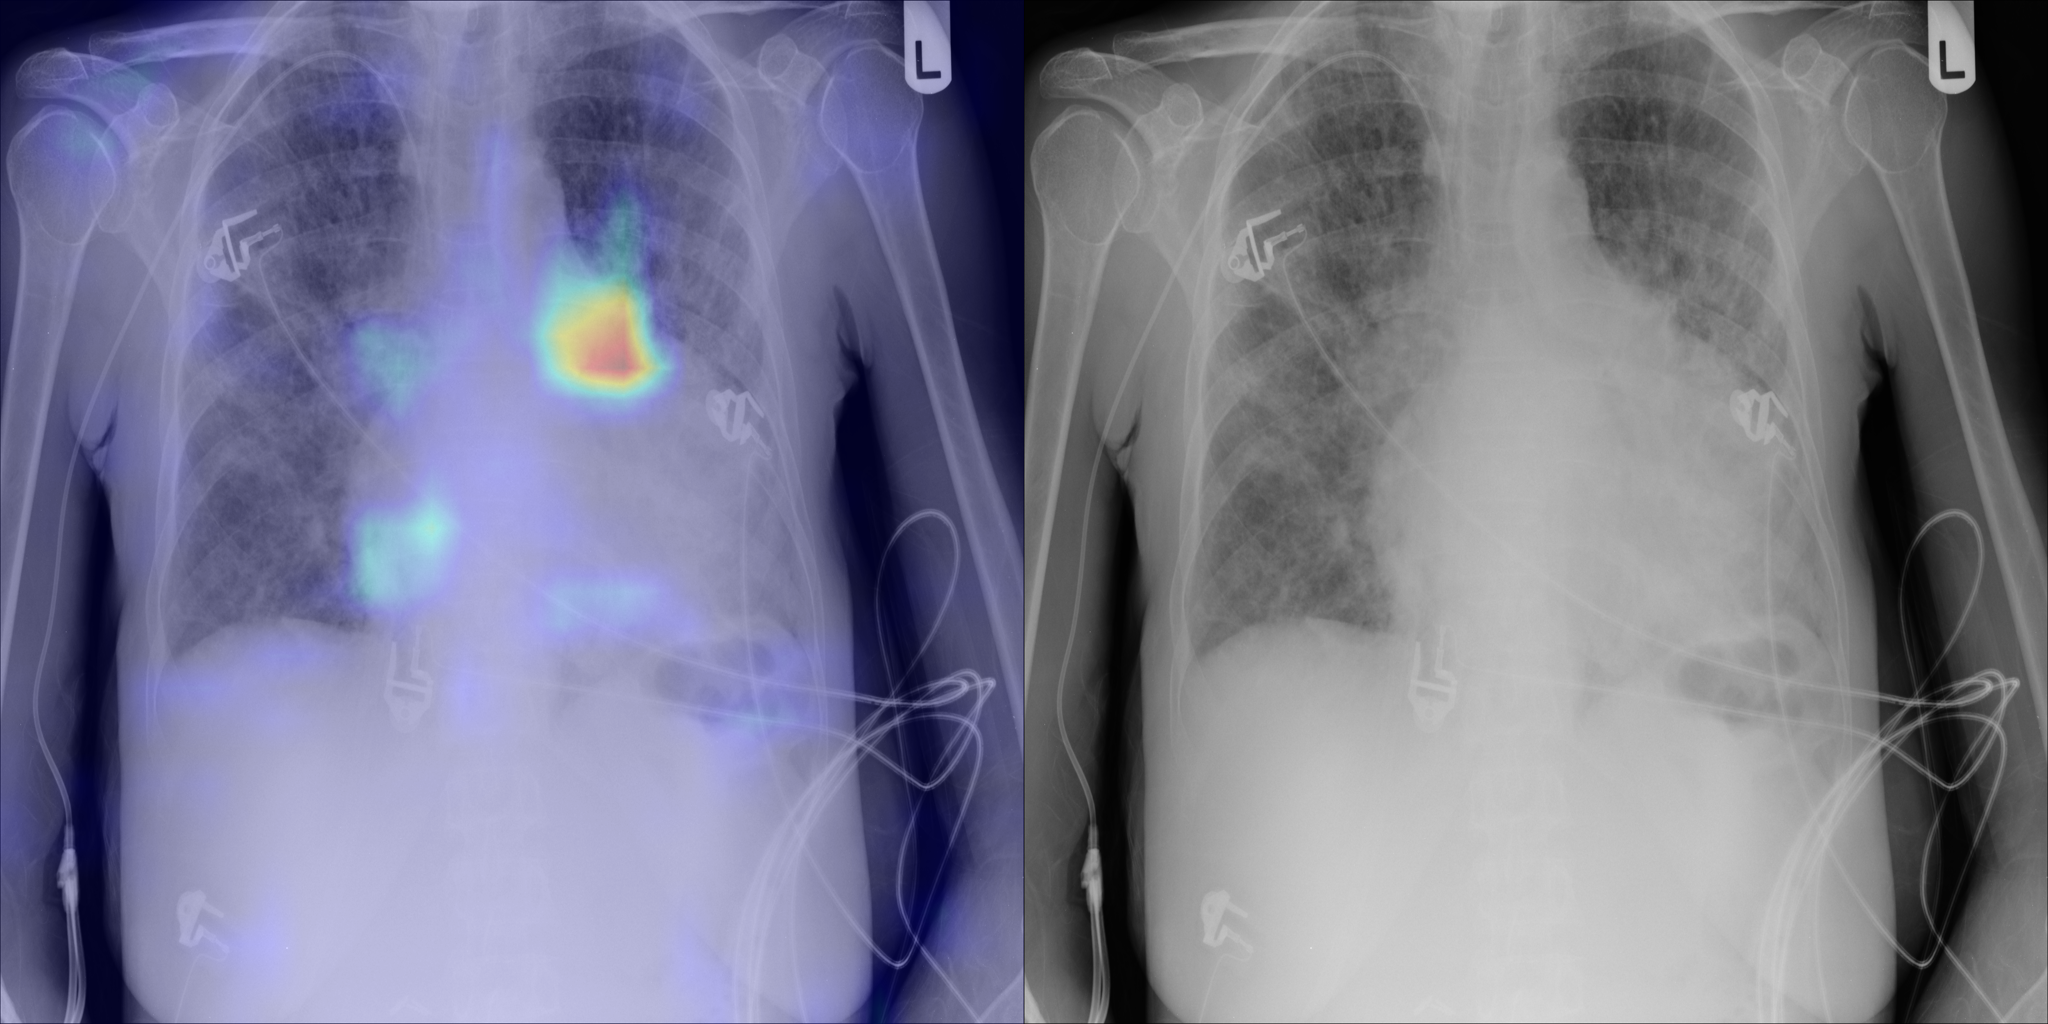
\includegraphics[width=1.0\textwidth]{Chapters/5. Conclusiones/img/Cardiomegaly/1_0_00004344_039.png}
    \end{subfigure}
    \begin{subfigure}{0.4\textwidth}
        \centering
        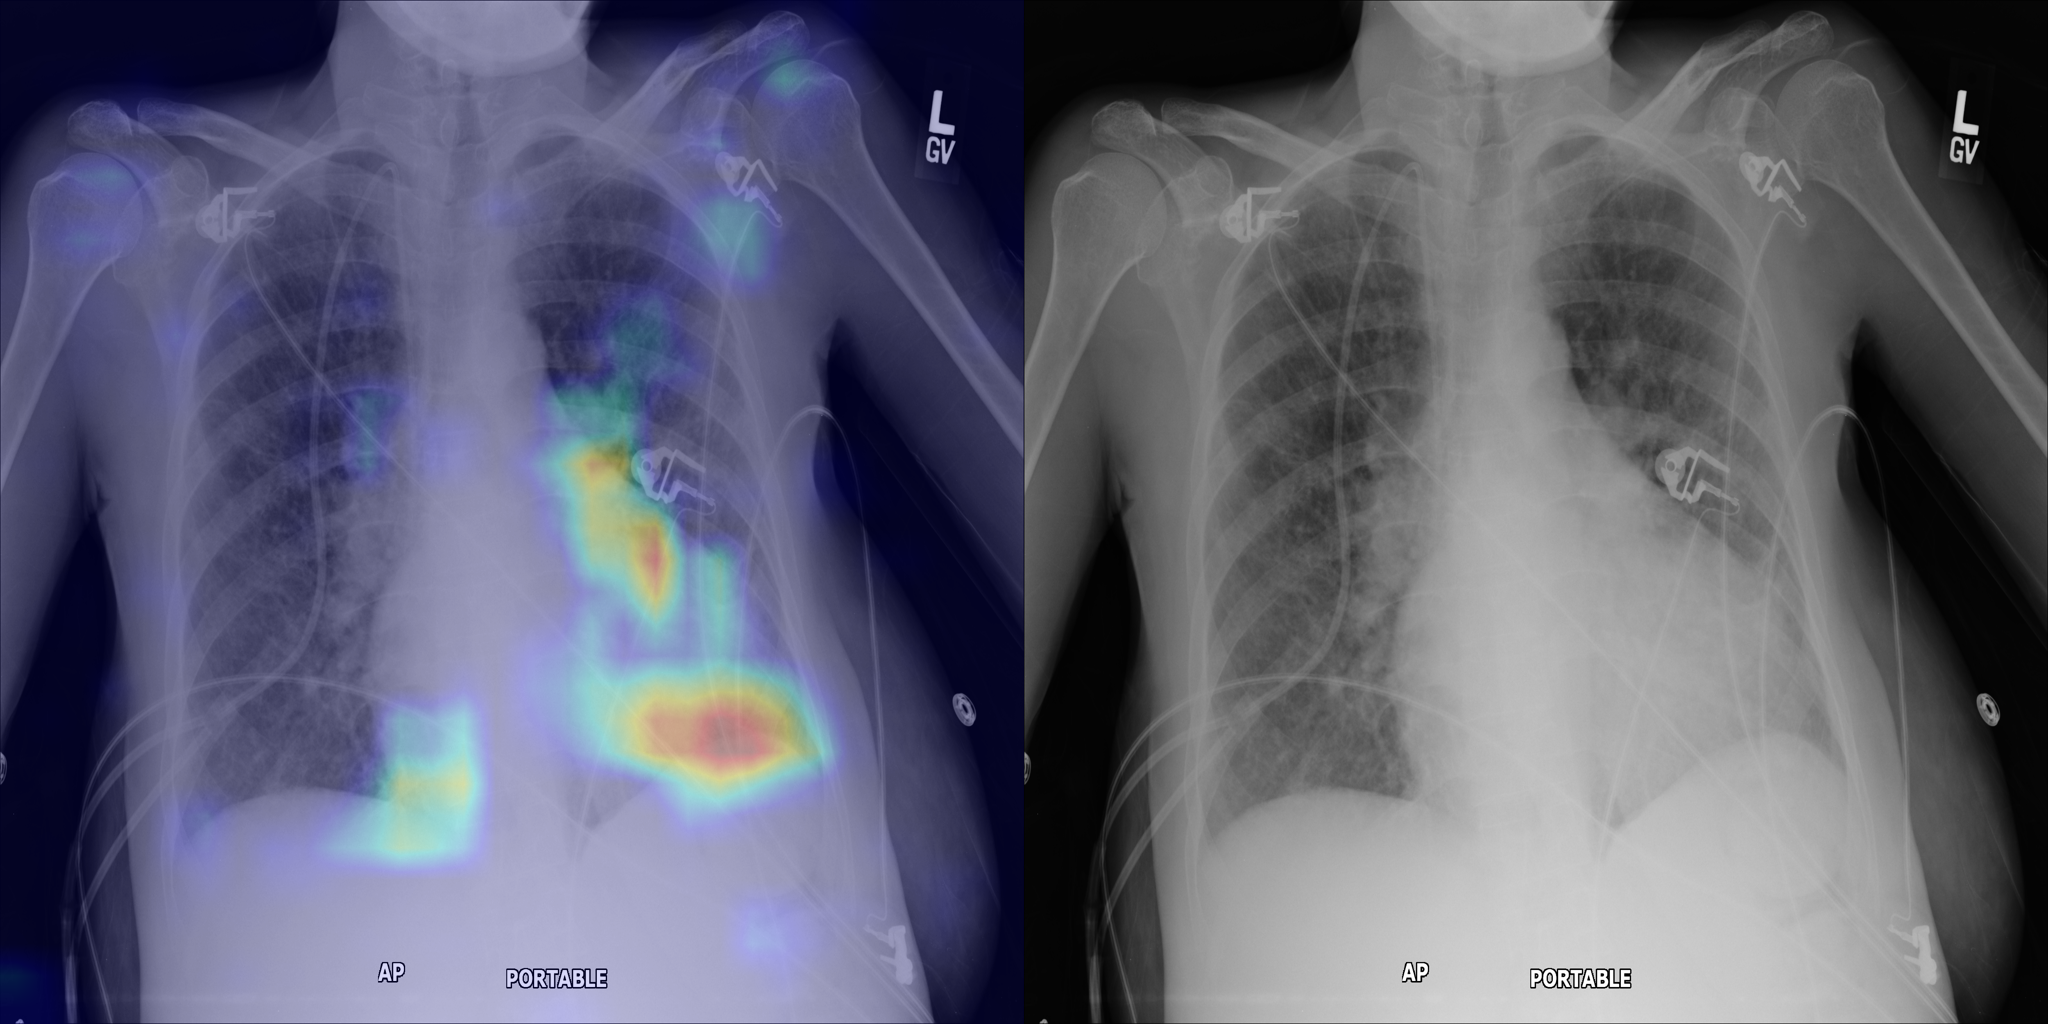
\includegraphics[width=1.0\textwidth]{Chapters/5. Conclusiones/img/Cardiomegaly/1_0_00004344_045.png}
    \end{subfigure}
    \begin{subfigure}{0.4\textwidth}
        \centering
        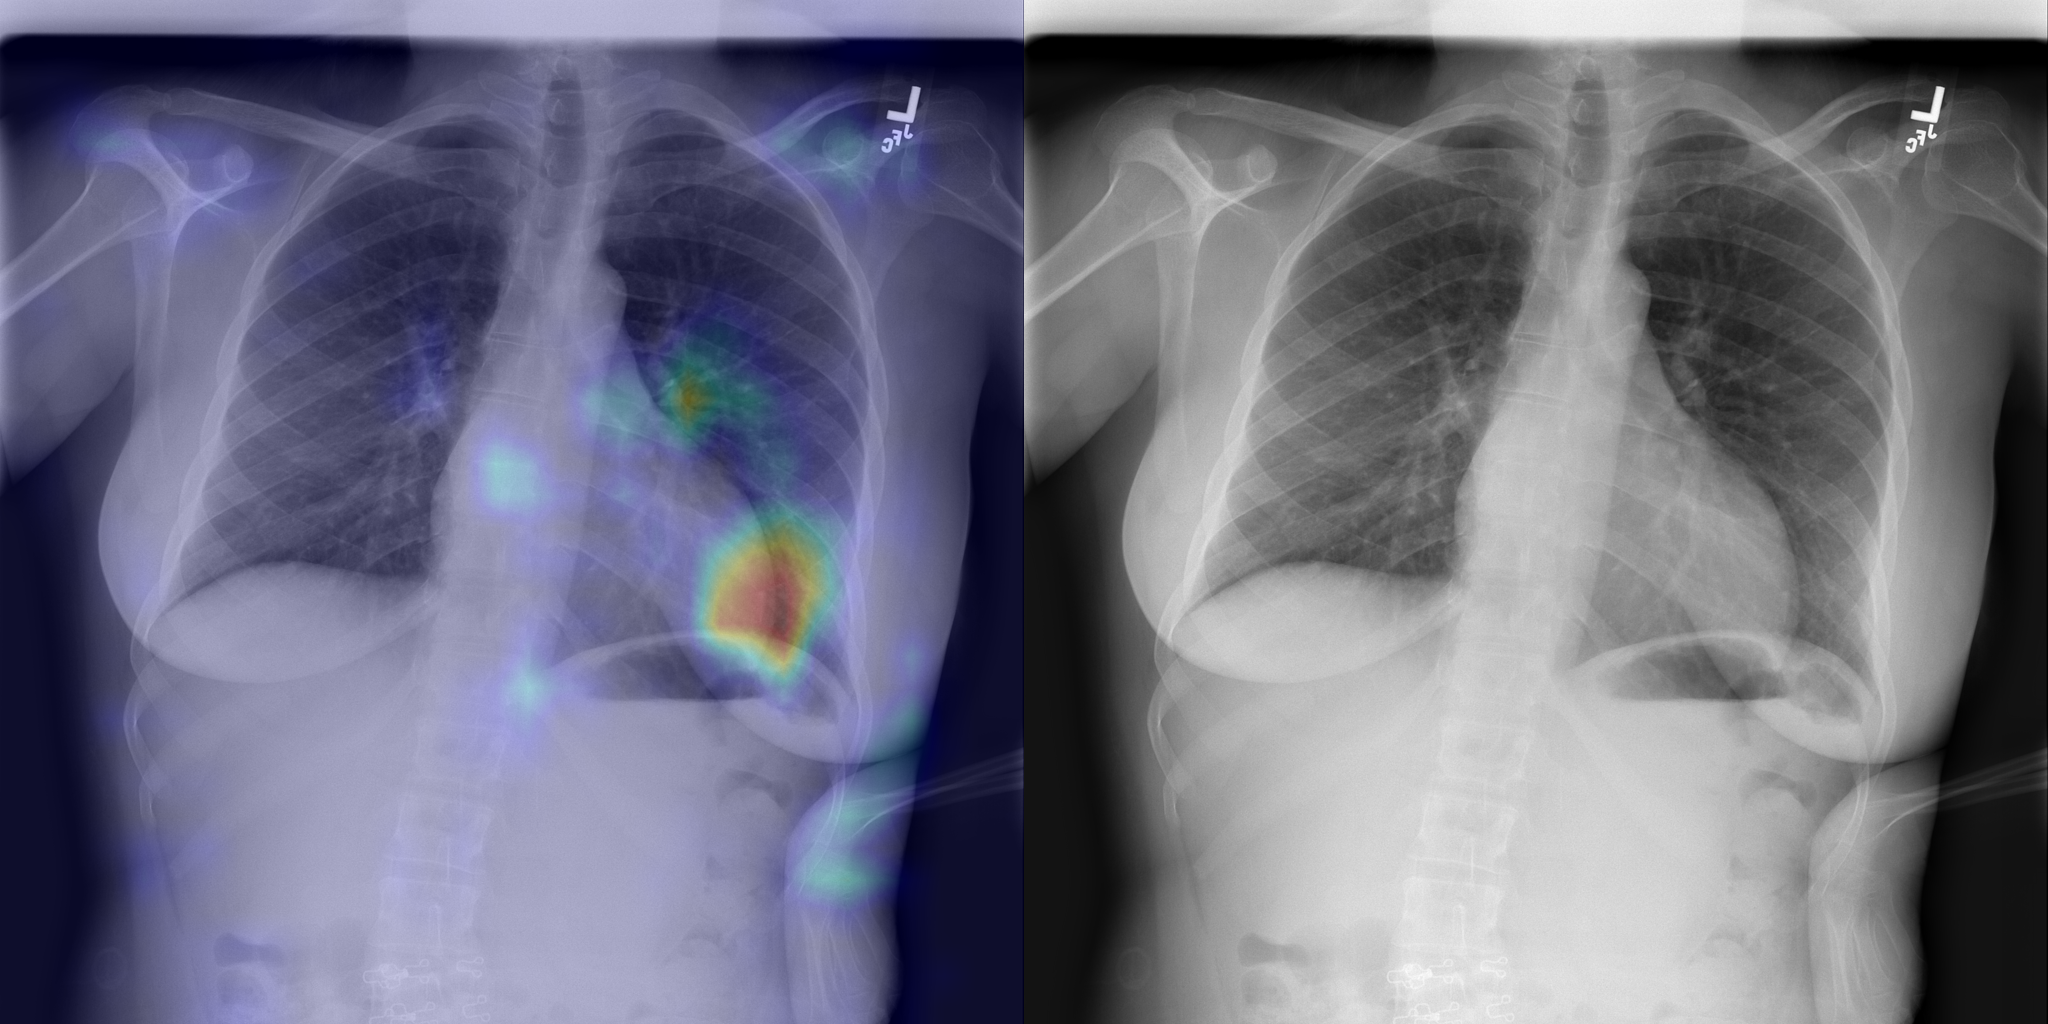
\includegraphics[width=1.0\textwidth]{Chapters/5. Conclusiones/img/Cardiomegaly/1_0_00004526_017.png}
    \end{subfigure}
    \begin{subfigure}{0.4\textwidth}
        \centering
        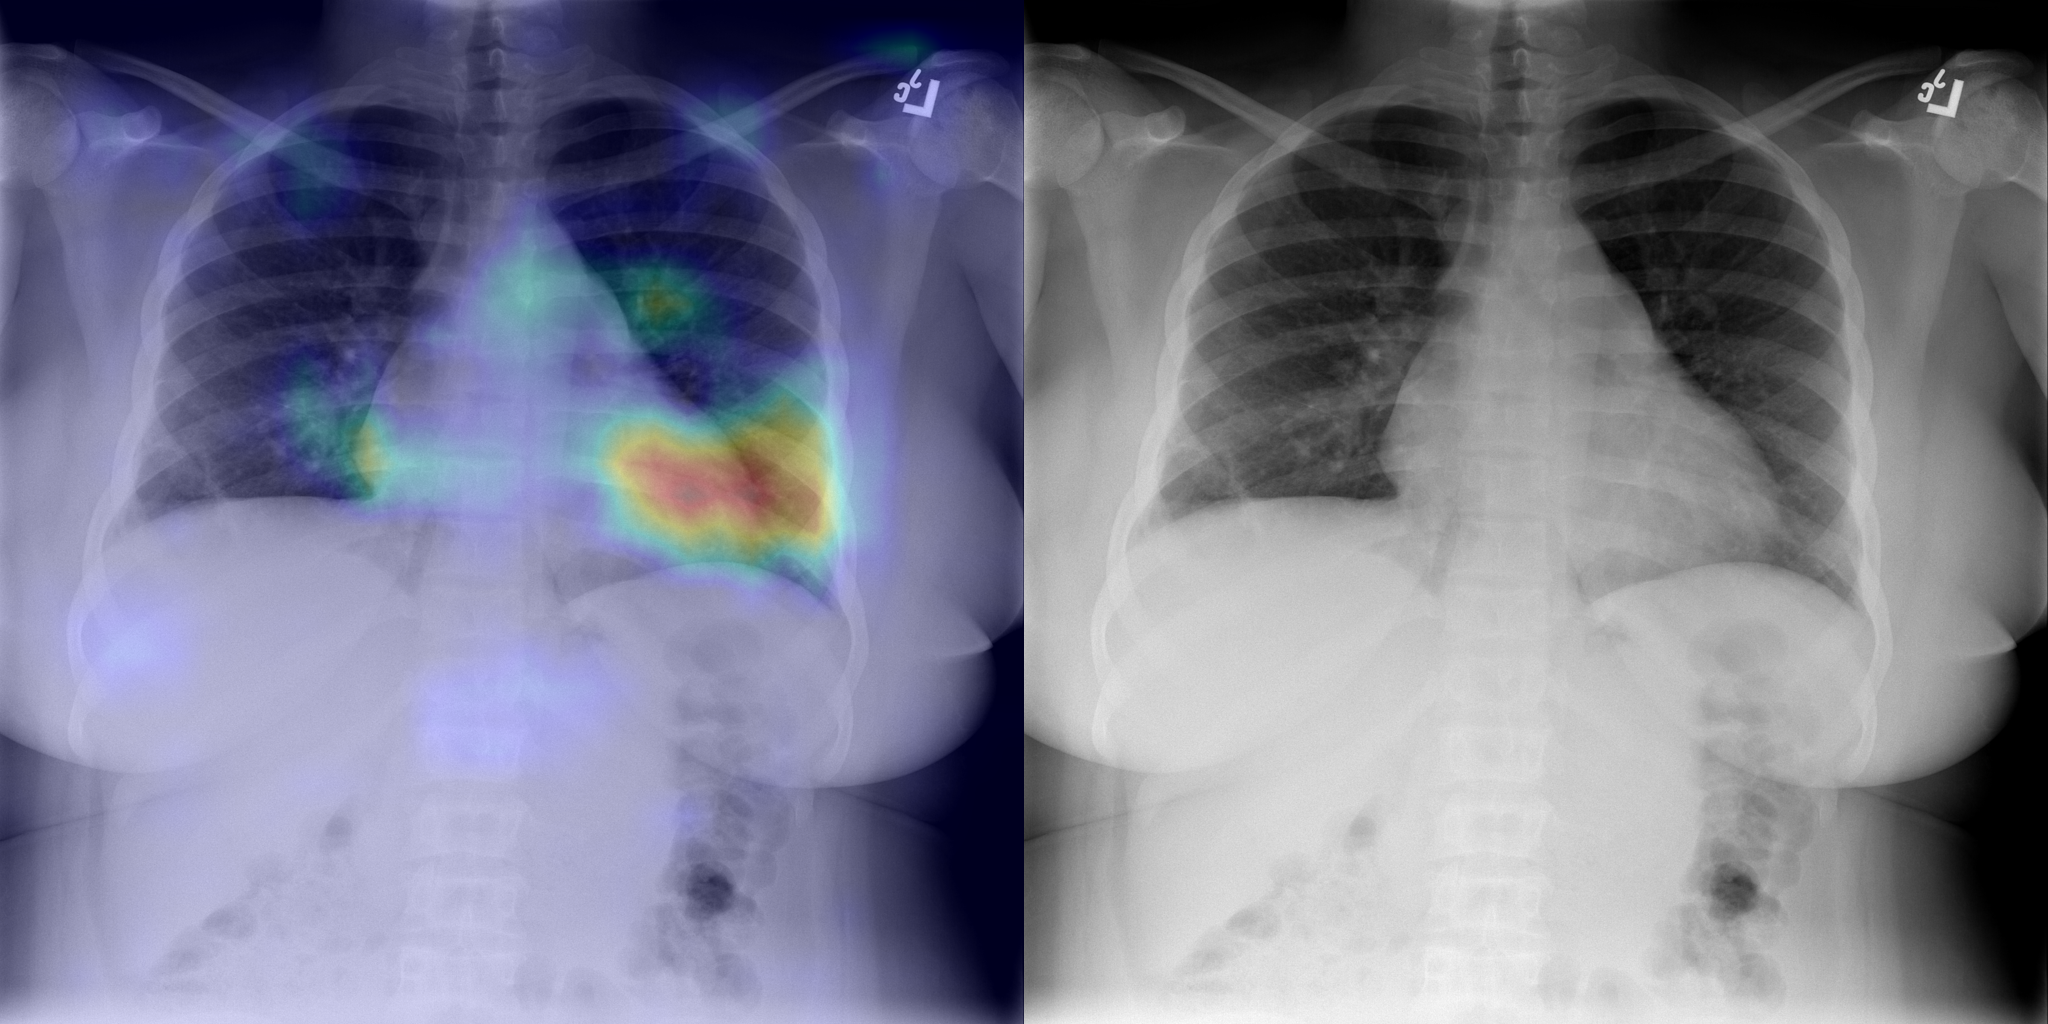
\includegraphics[width=1.0\textwidth]{Chapters/5. Conclusiones/img/Cardiomegaly/1_1_00014706_010.png}
    \end{subfigure}
    \begin{subfigure}{0.4\textwidth}
        \centering
        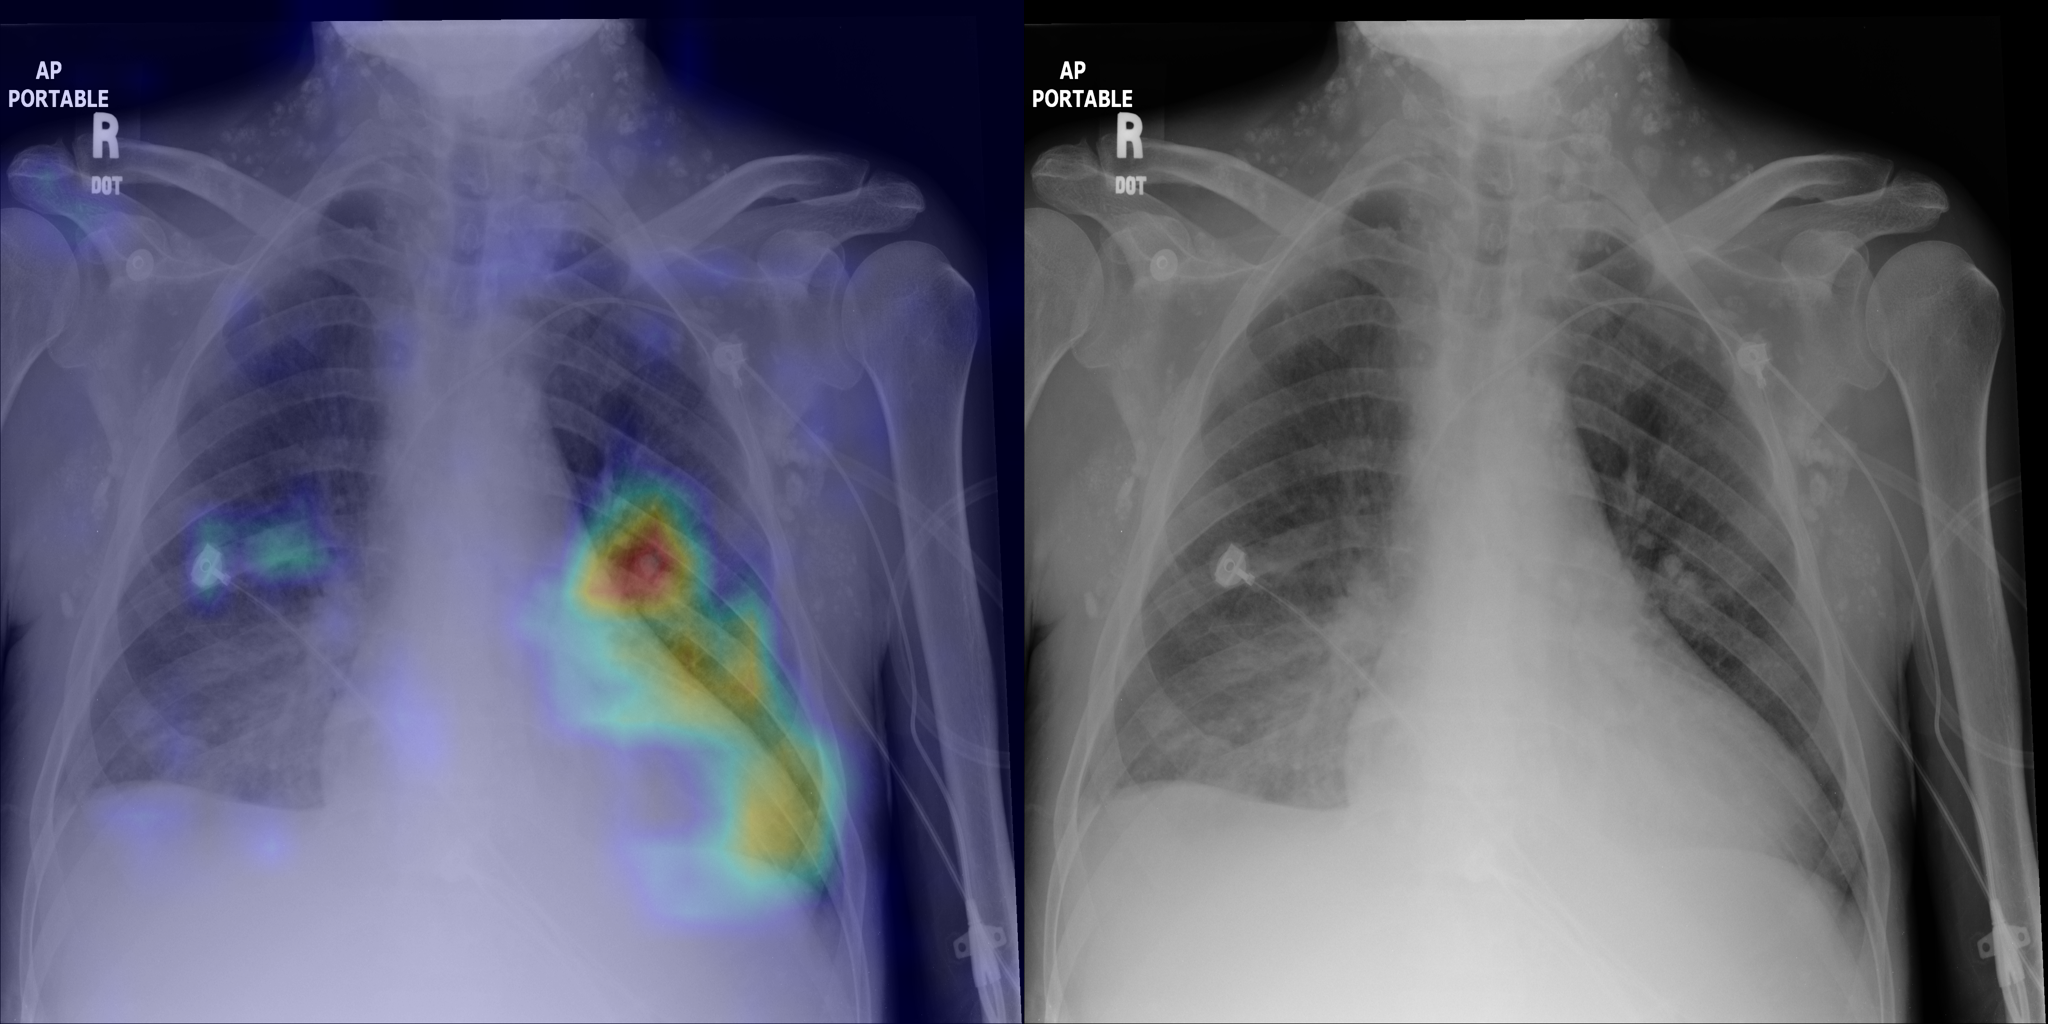
\includegraphics[width=1.0\textwidth]{Chapters/5. Conclusiones/img/Cardiomegaly/1_1_00016291_042.png}
    \end{subfigure}

    \caption{Cardiomegalia. Radiografías detectadas con la patología de cardiomegalia por los
                    radiólogos. A la izquierda de cada imagen el GradCam correspondiente a la detección
                    de la patología como positivo por el modelo CNN.}

    \label{fig-cardiomegalia}
\end{figure}

\begin{figure}[b]
    \centering
    \begin{subfigure}{0.4\textwidth}
        \centering
        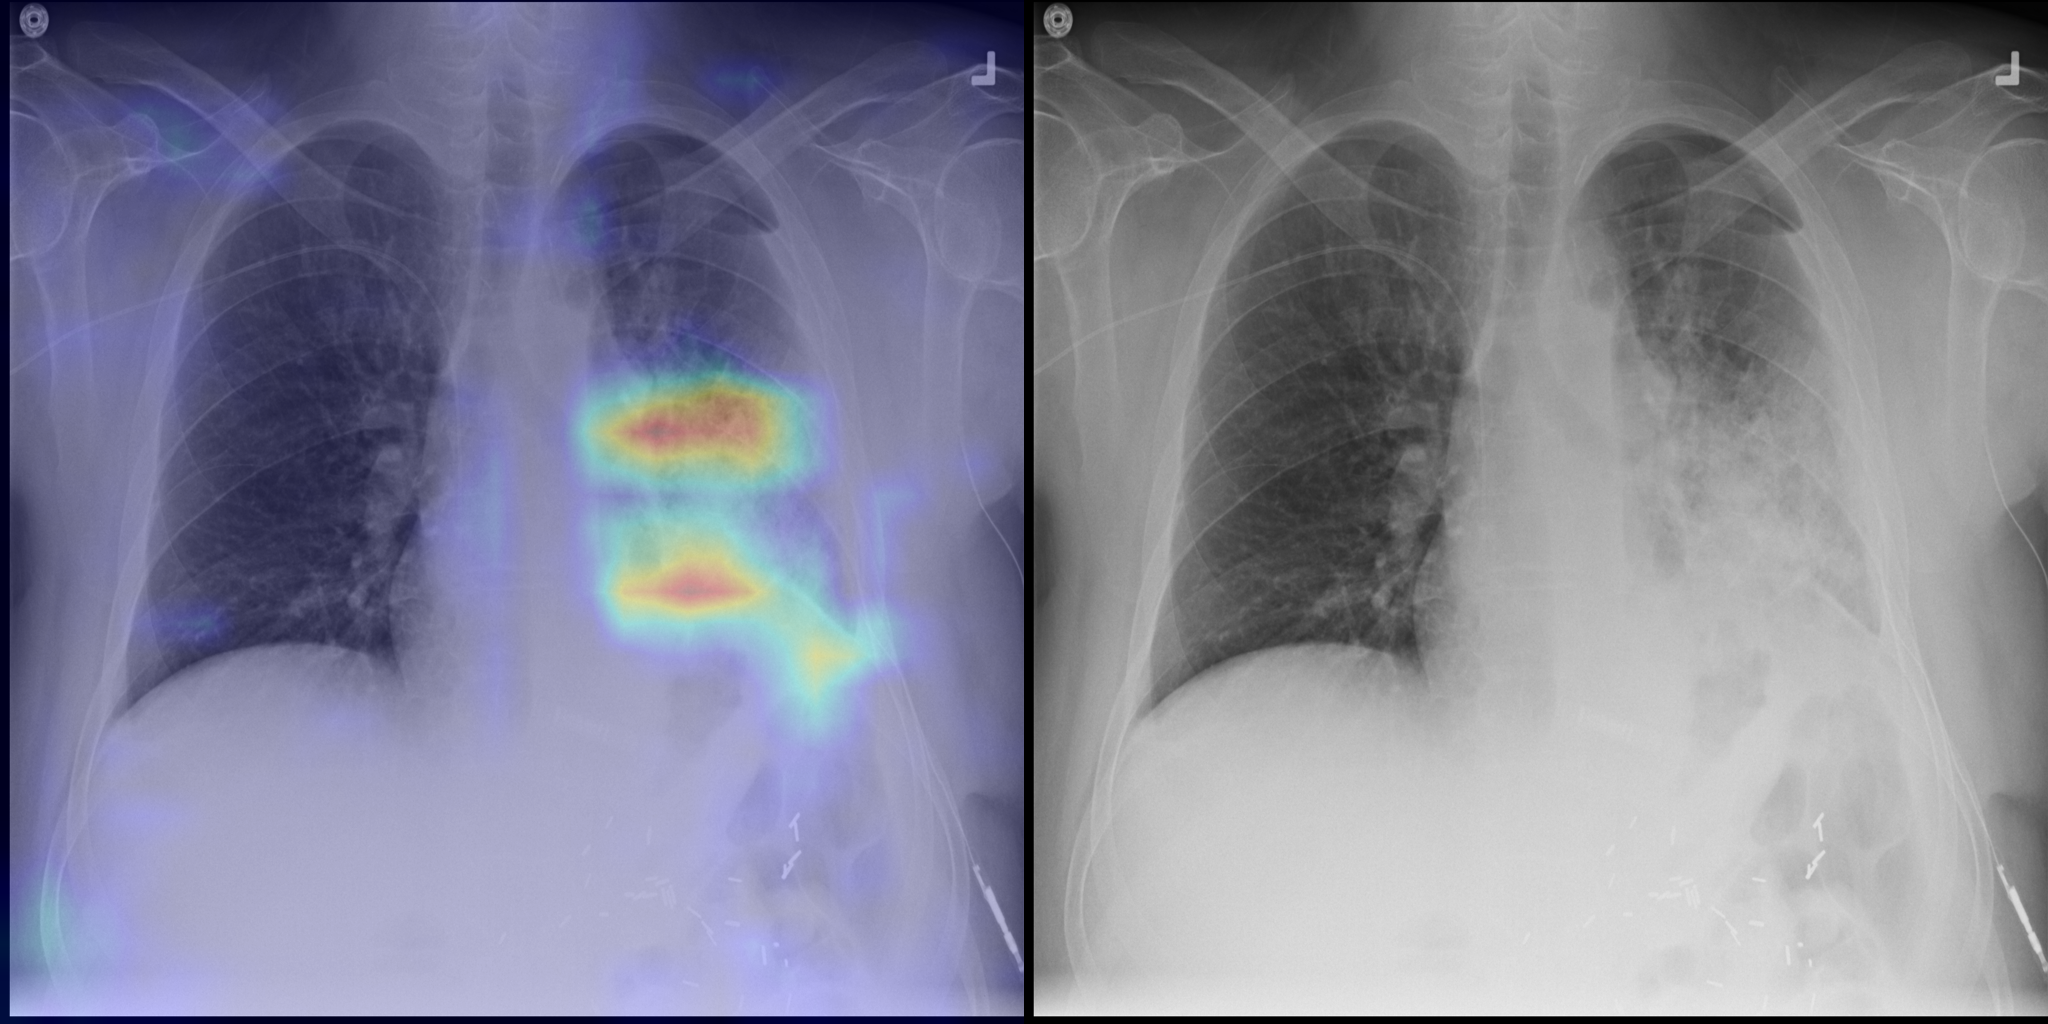
\includegraphics[width=1.0\textwidth]{Chapters/5. Conclusiones/img/Consolidation/1_1_00000246_014.png}
    \end{subfigure}
    \begin{subfigure}{0.4\textwidth}
        \centering
        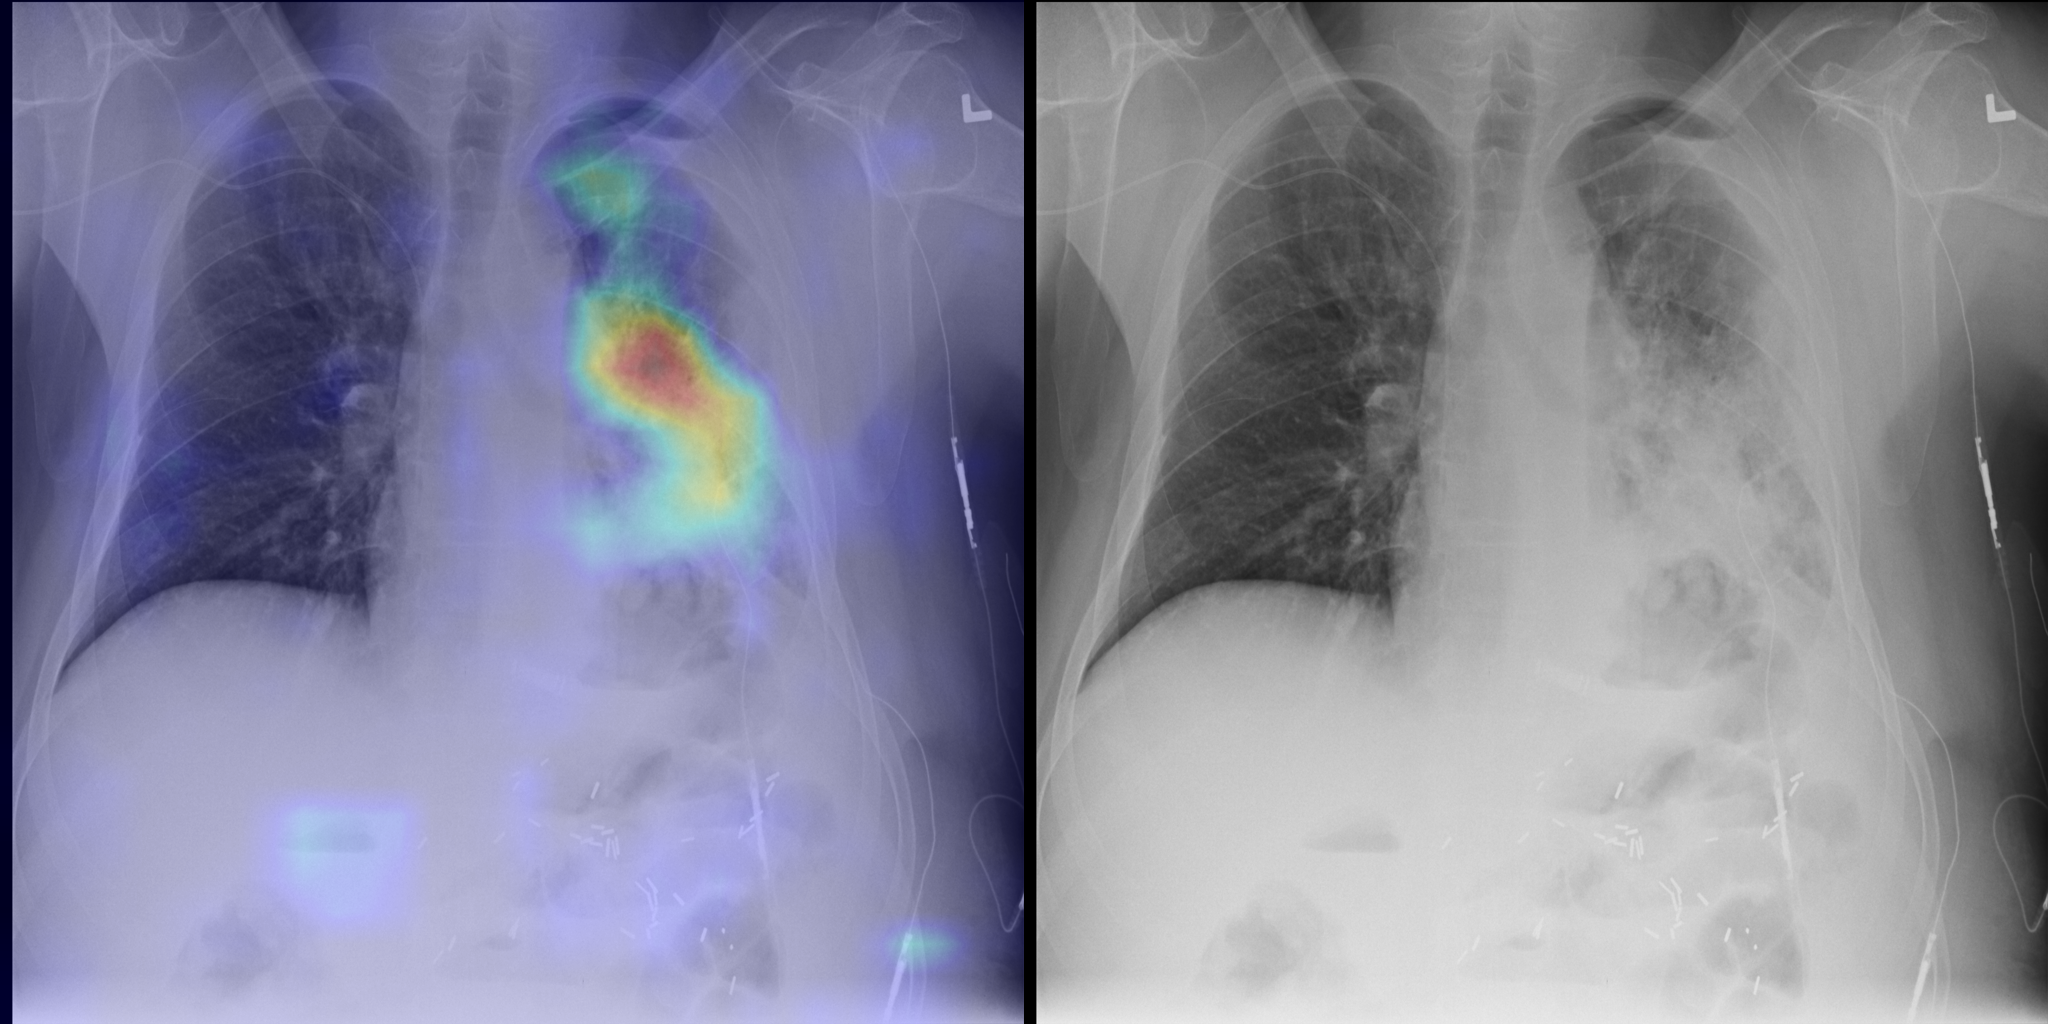
\includegraphics[width=1.0\textwidth]{Chapters/5. Conclusiones/img/Consolidation/1_1_00000246_016.png}
    \end{subfigure}
    \begin{subfigure}{0.4\textwidth}
        \centering
        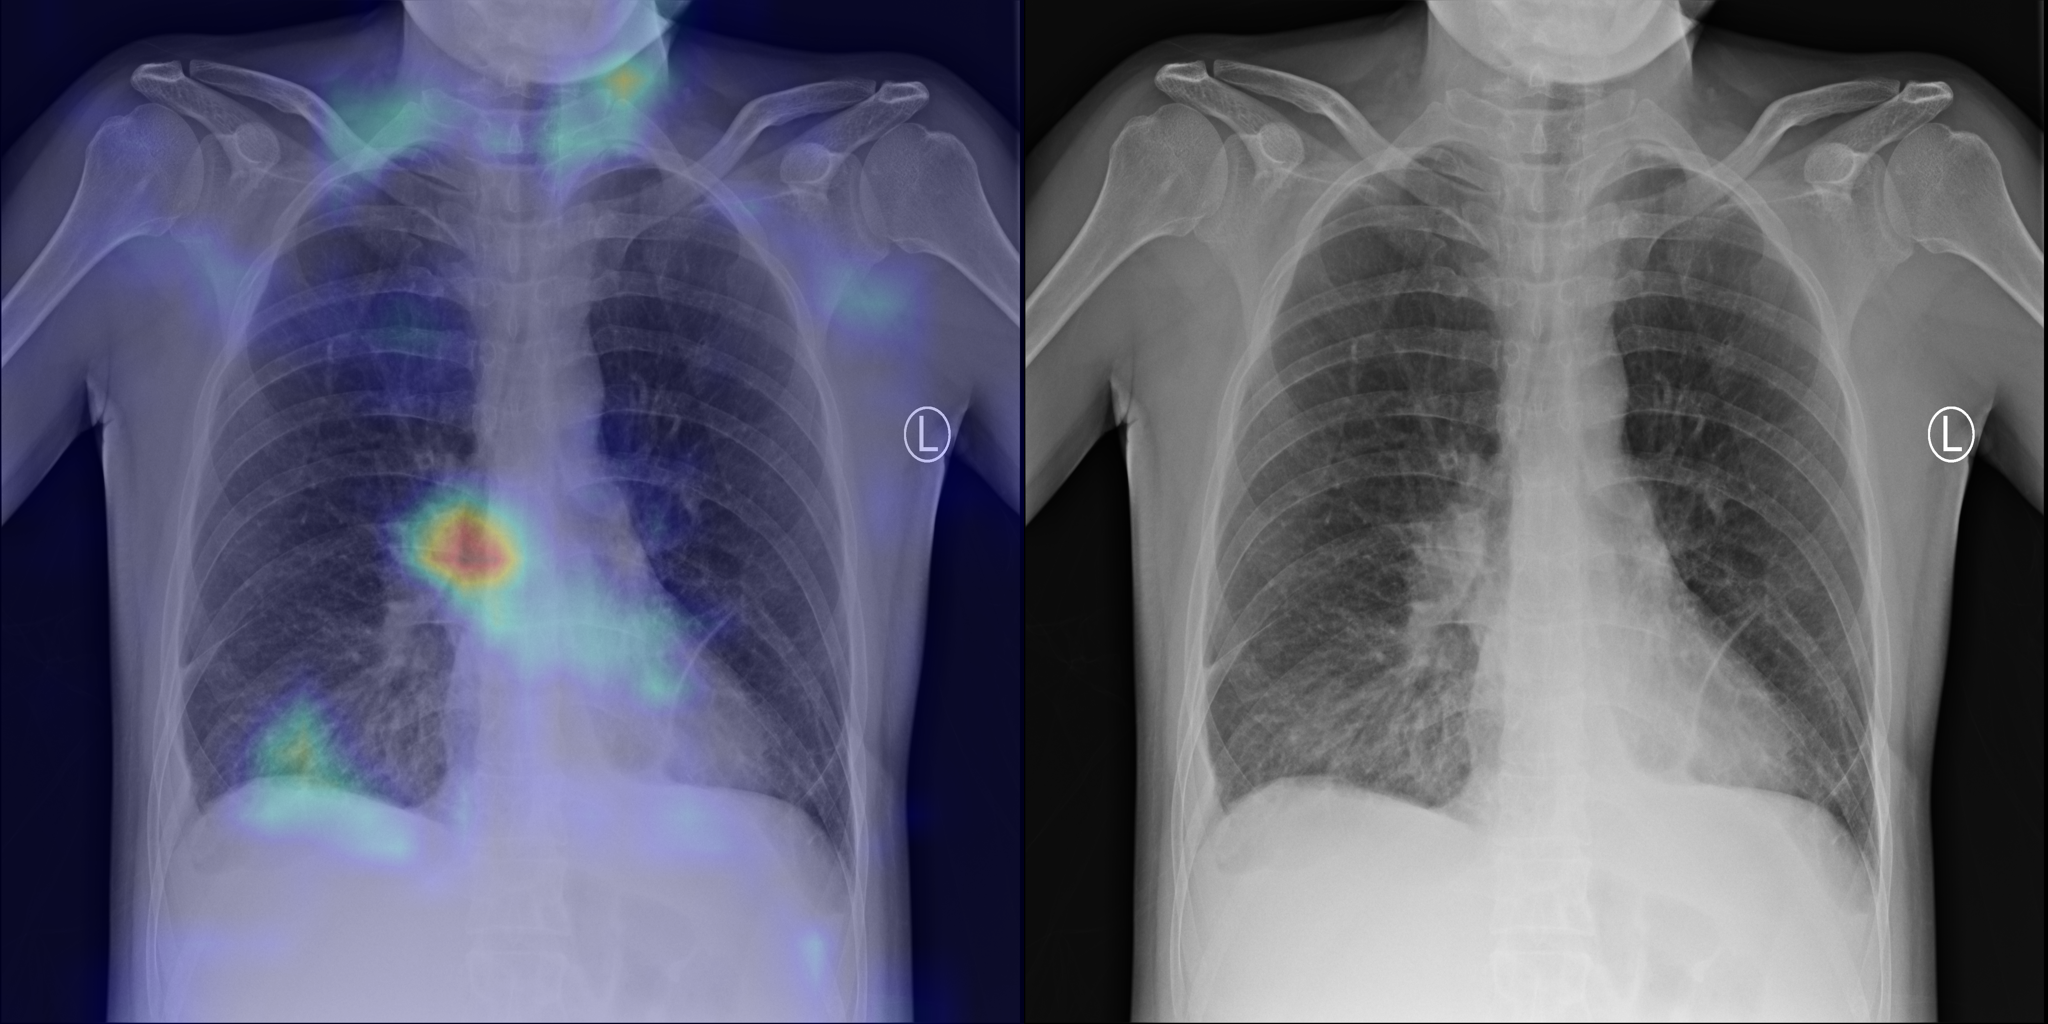
\includegraphics[width=1.0\textwidth]{Chapters/5. Conclusiones/img/Consolidation/1_1_00000344_000.png}
    \end{subfigure}
    \begin{subfigure}{0.4\textwidth}
        \centering
        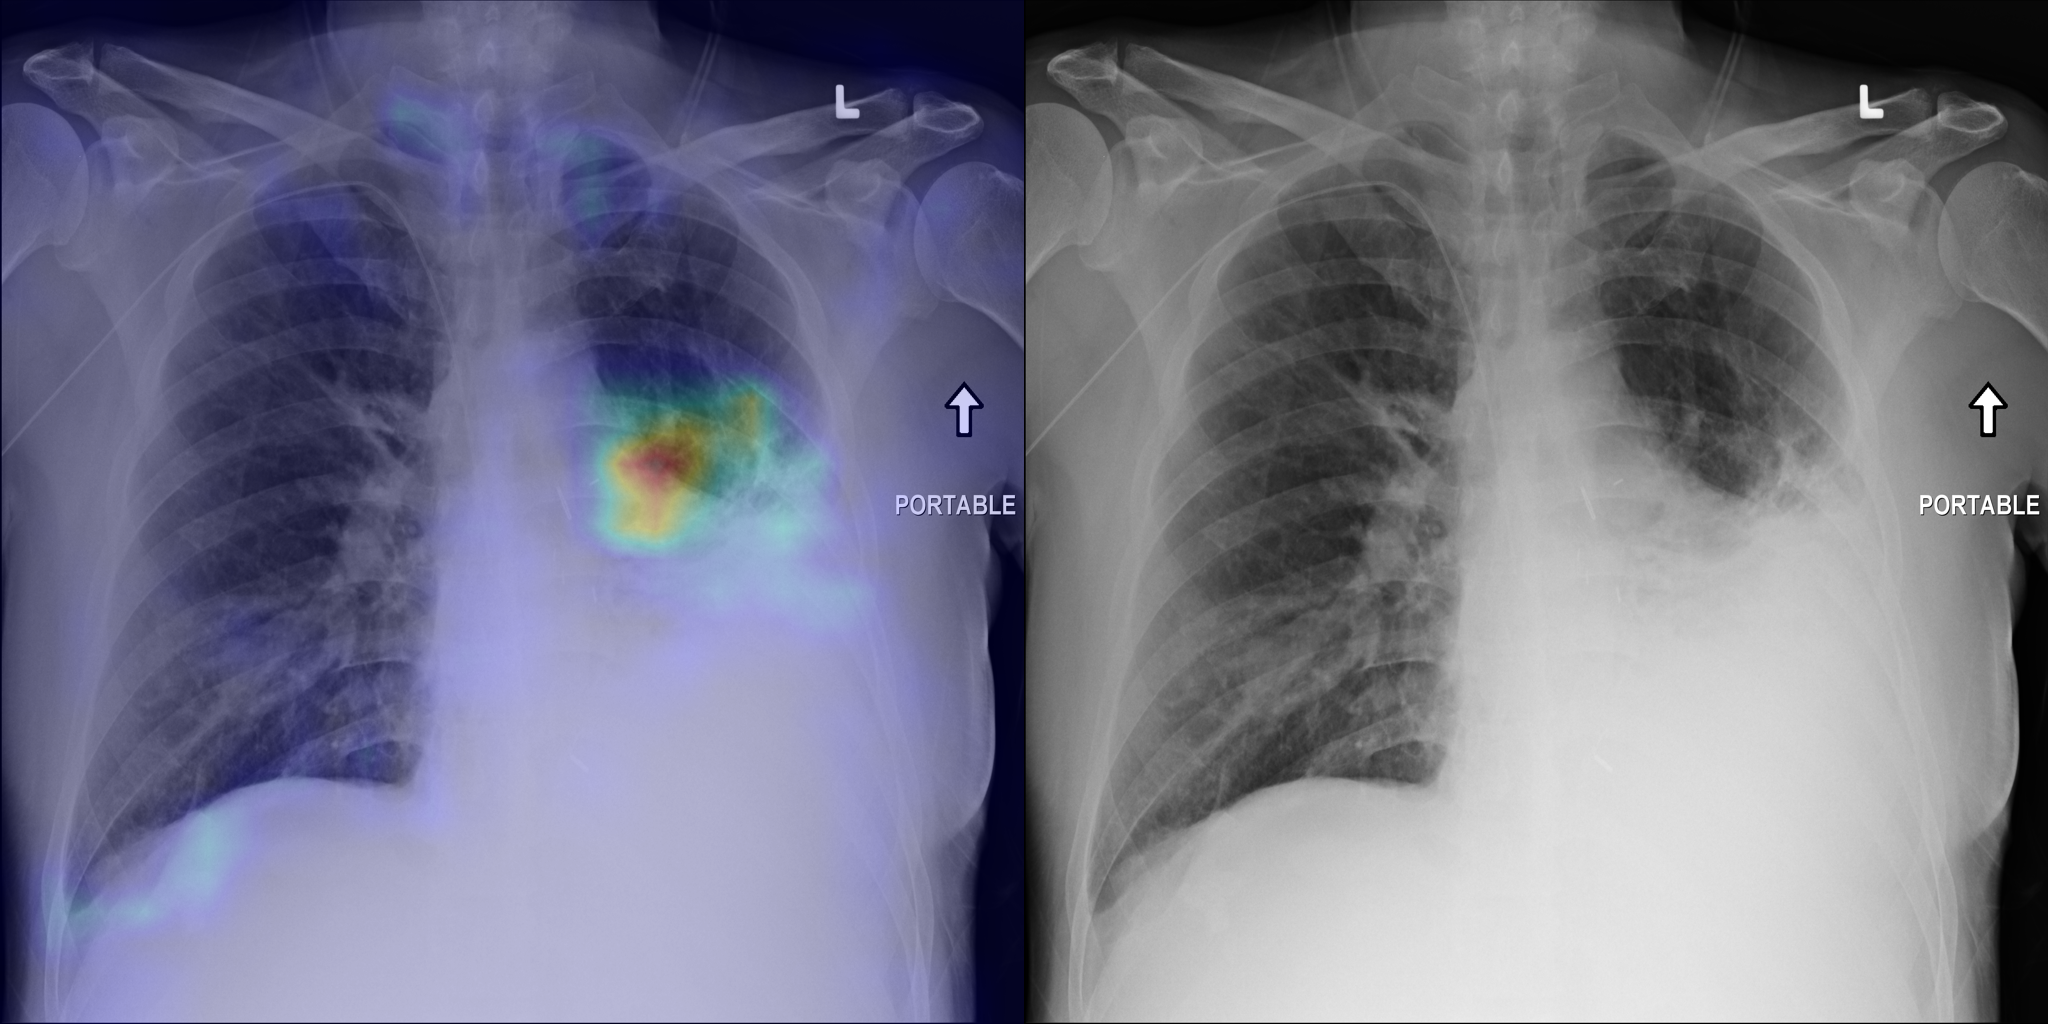
\includegraphics[width=1.0\textwidth]{Chapters/5. Conclusiones/img/Consolidation/1_1_00000467_002.png}
    \end{subfigure}
    \begin{subfigure}{0.4\textwidth}
        \centering
        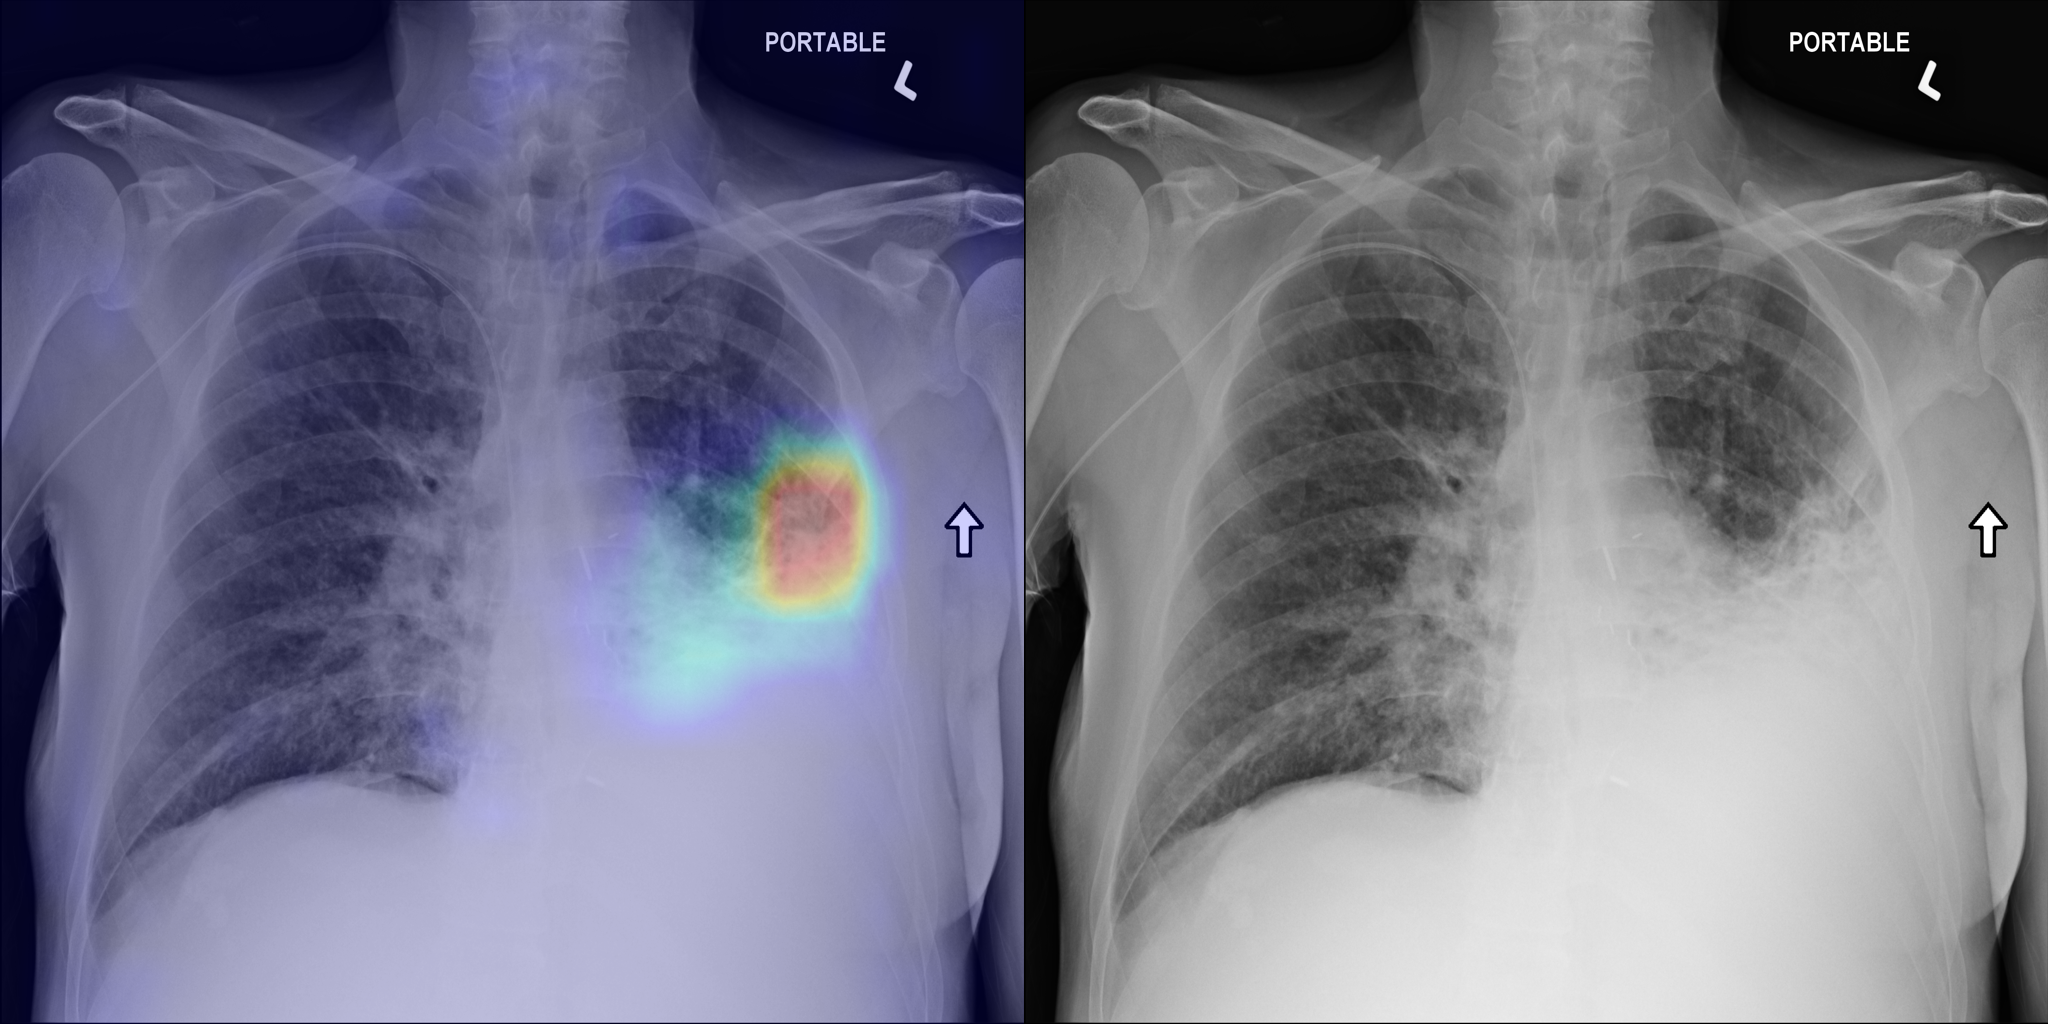
\includegraphics[width=1.0\textwidth]{Chapters/5. Conclusiones/img/Consolidation/1_1_00000467_003.png}
    \end{subfigure}
    \begin{subfigure}{0.4\textwidth}
        \centering
        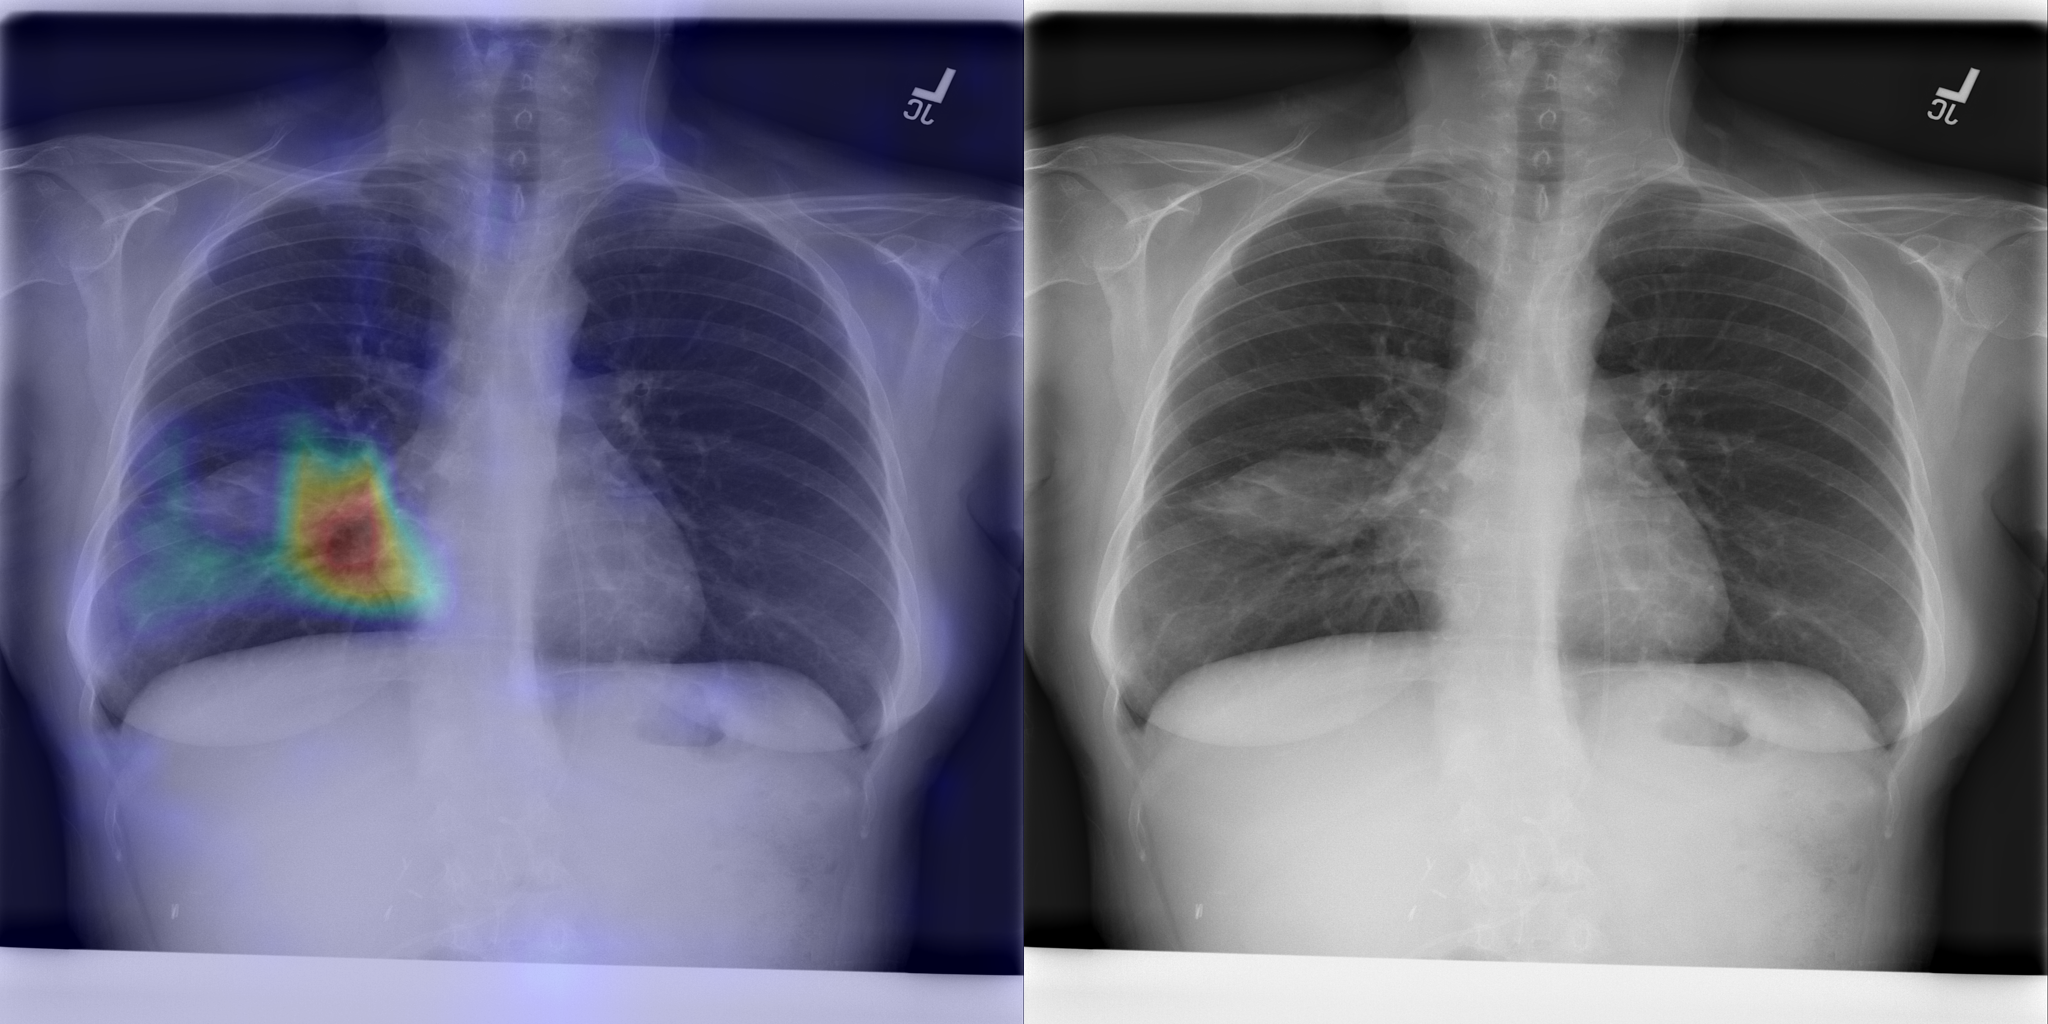
\includegraphics[width=1.0\textwidth]{Chapters/5. Conclusiones/img/Consolidation/1_1_00000618_008.png}
    \end{subfigure}
    \begin{subfigure}{0.4\textwidth}
        \centering
        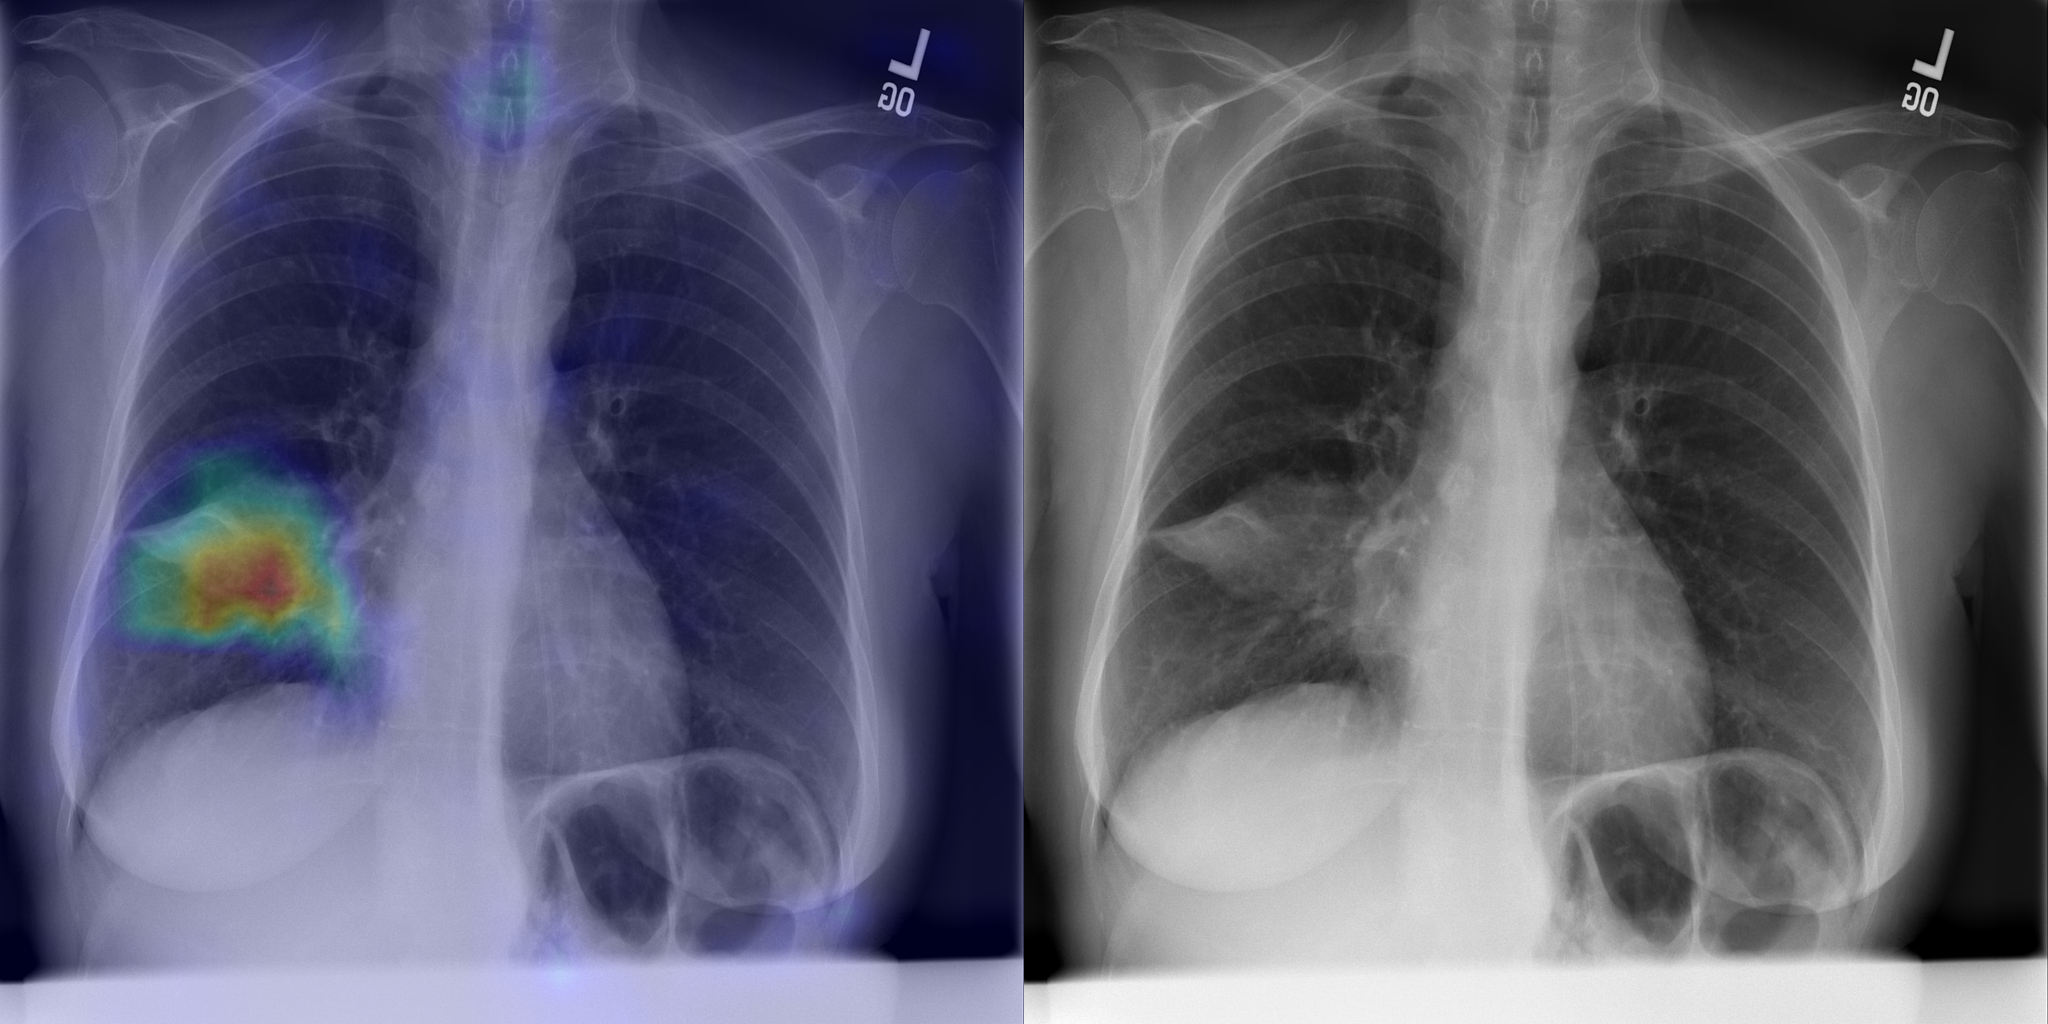
\includegraphics[width=1.0\textwidth]{Chapters/5. Conclusiones/img/Consolidation/1_1_00000618_011.png}
    \end{subfigure}
    \begin{subfigure}{0.4\textwidth}
        \centering
        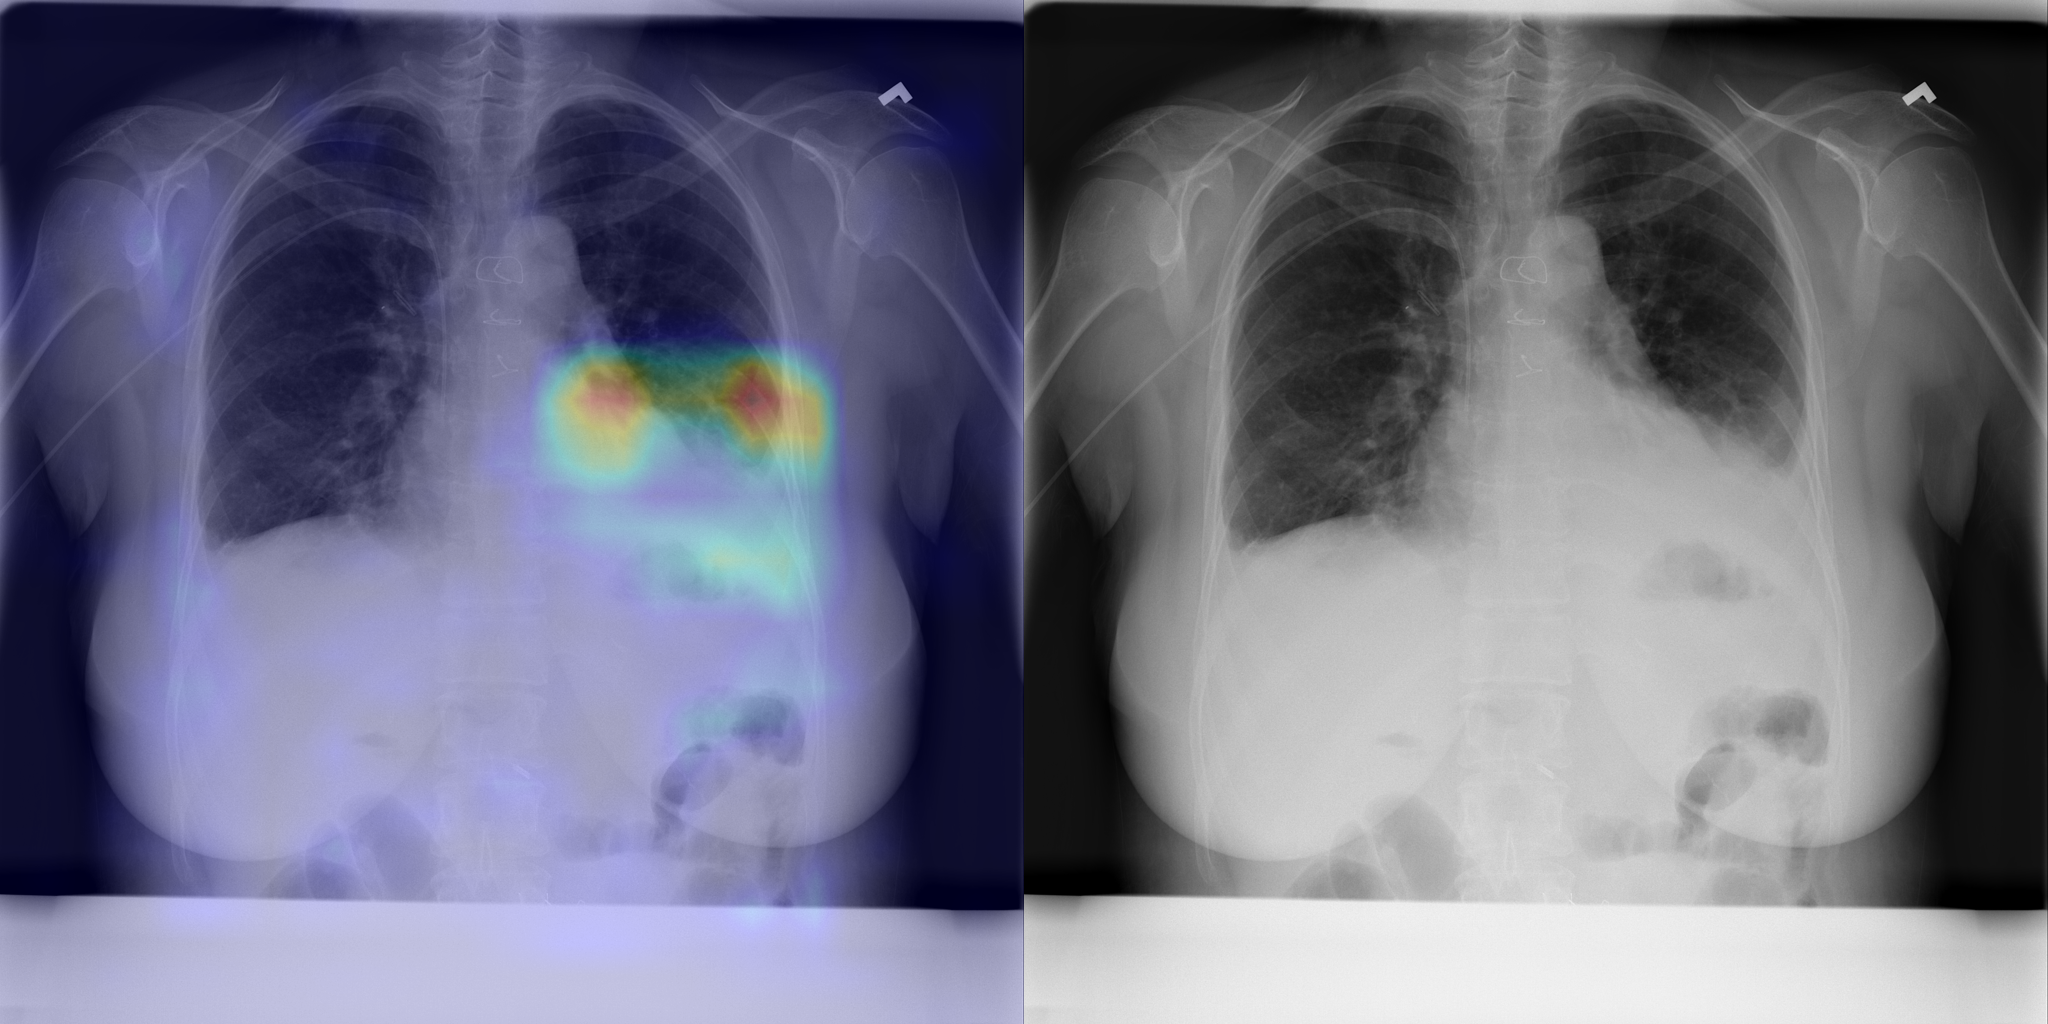
\includegraphics[width=1.0\textwidth]{Chapters/5. Conclusiones/img/Consolidation/1_1_00000808_002.png}
    \end{subfigure}
    \begin{subfigure}{0.4\textwidth}
        \centering
        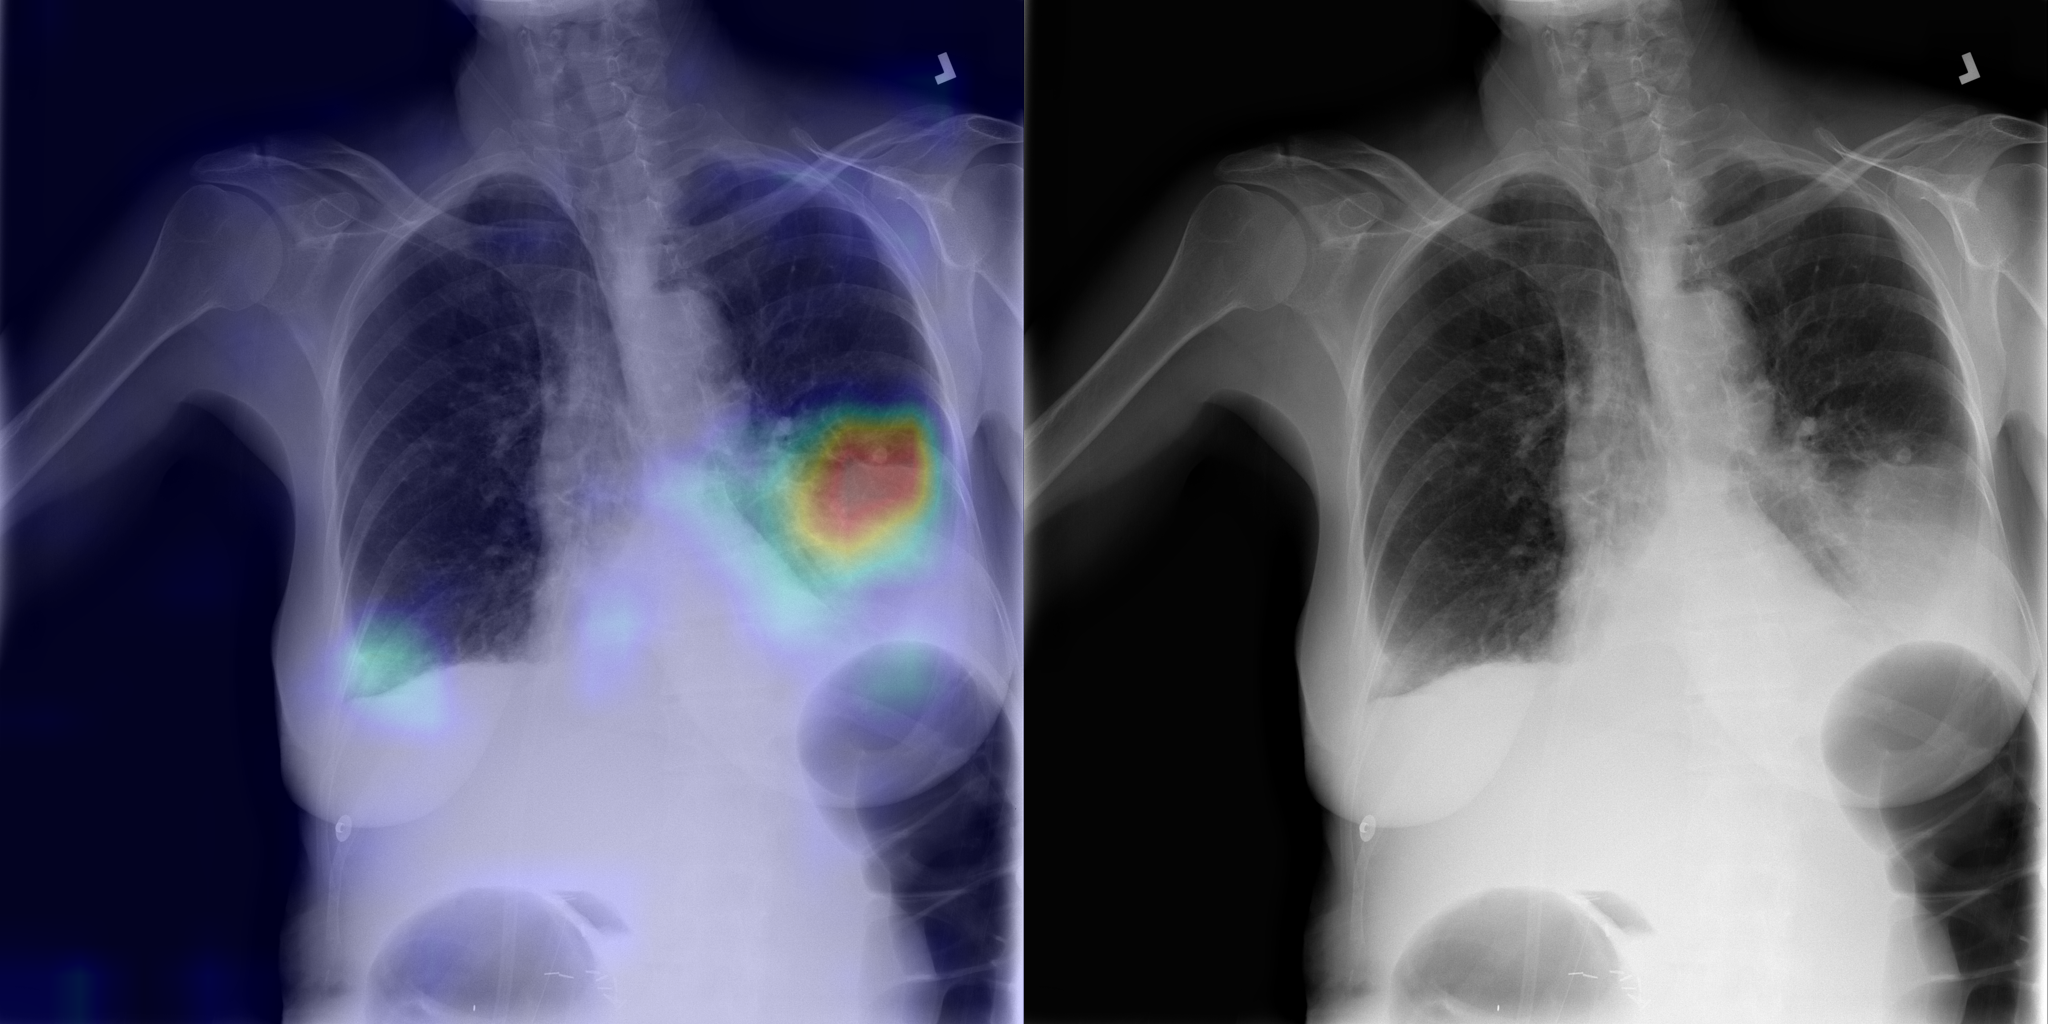
\includegraphics[width=1.0\textwidth]{Chapters/5. Conclusiones/img/Consolidation/1_1_00000882_003.png}
    \end{subfigure}
    \begin{subfigure}{0.4\textwidth}
        \centering
        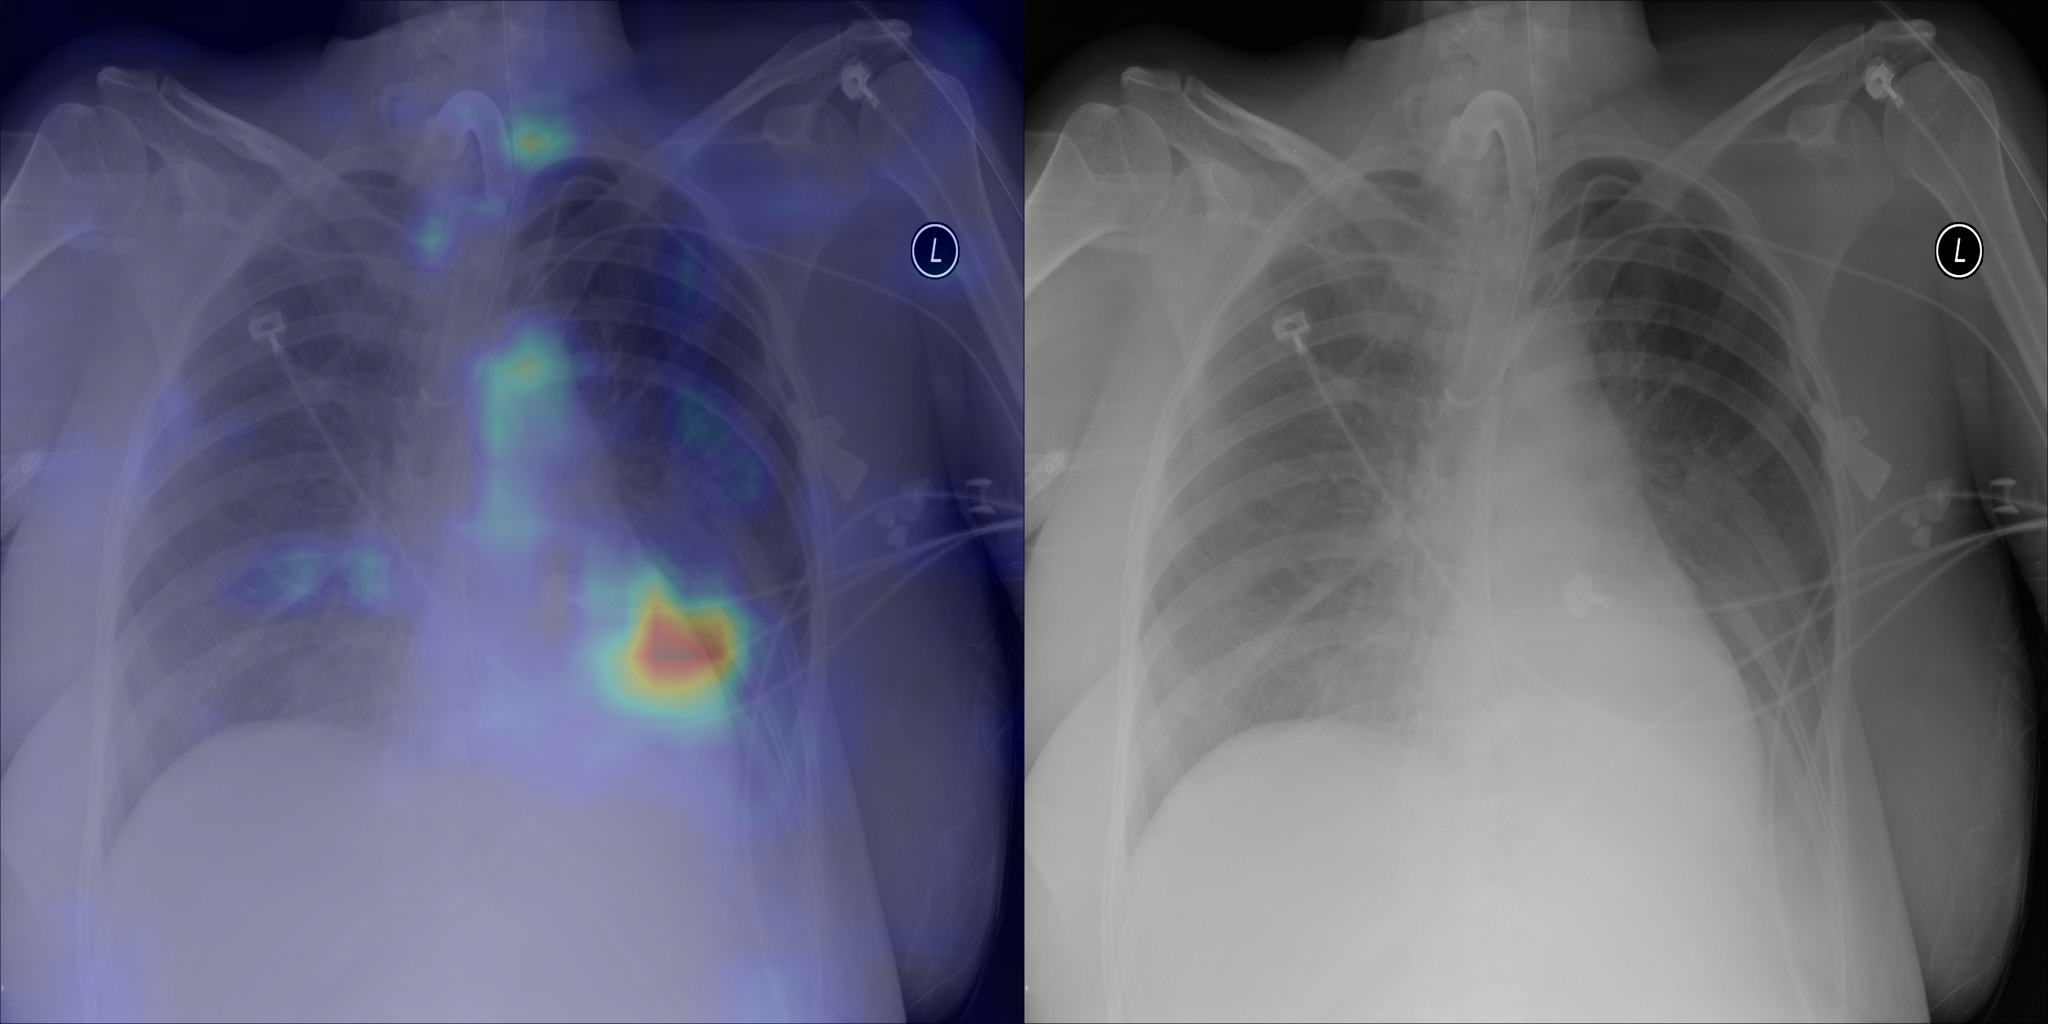
\includegraphics[width=1.0\textwidth]{Chapters/5. Conclusiones/img/Consolidation/1_1_00018187_052.png}
    \end{subfigure}

    \caption{Consolidación pulmunar. Radiografías detectadas con la patología de consolidación pulmunar por los
                    radiólogos. A la izquierda de cada imagen el GradCam correspondiente a la detección
                    de la patología como positivo por el modelo CNN.}
\end{figure}

\begin{figure}[b]
    \centering
    \begin{subfigure}{0.4\textwidth}
        \centering
        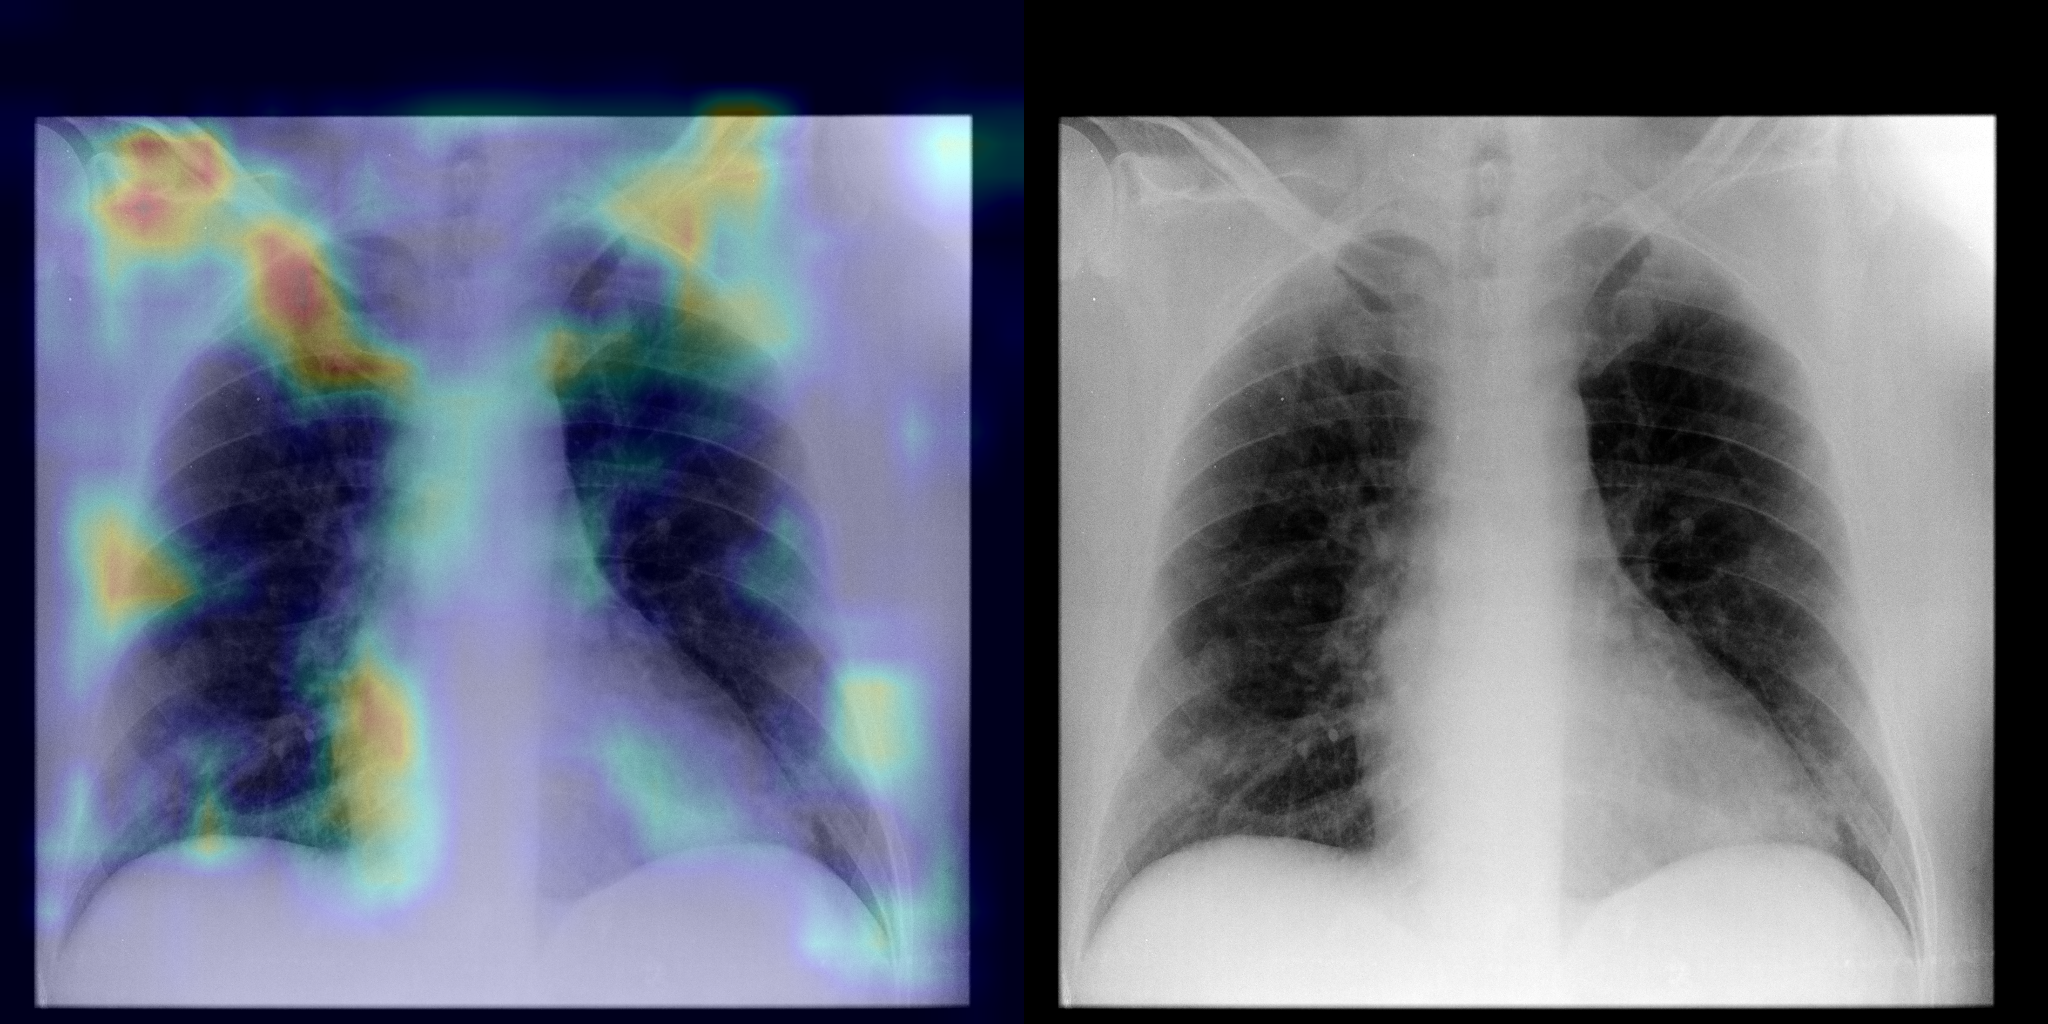
\includegraphics[width=1.0\textwidth]{Chapters/5. Conclusiones/img/COVID-19/1_1_0c9b15035c41_3ea703bd1e0b.png}
    \end{subfigure}
    \begin{subfigure}{0.4\textwidth}
        \centering
        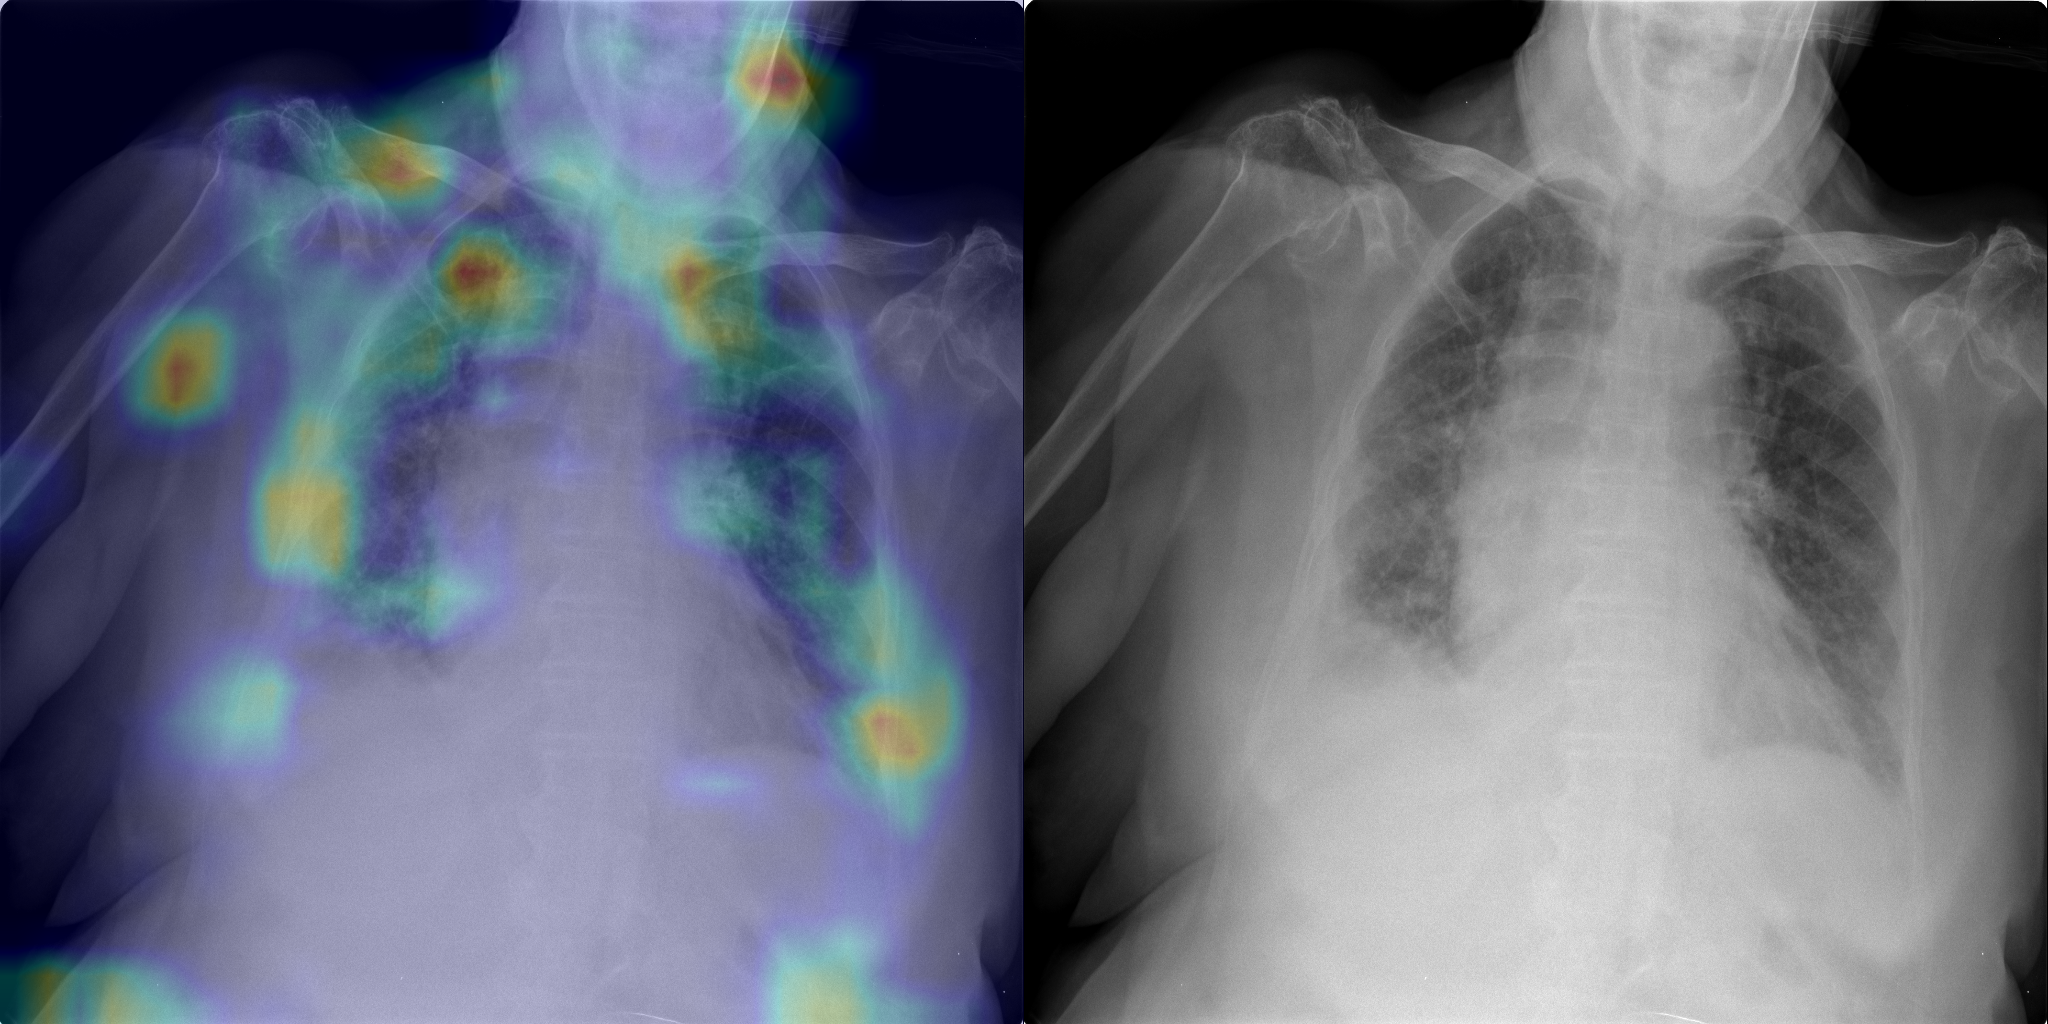
\includegraphics[width=1.0\textwidth]{Chapters/5. Conclusiones/img/COVID-19/1_1_0d5082a9a044_d417f8e64511.png}
    \end{subfigure}
    \begin{subfigure}{0.4\textwidth}
        \centering
        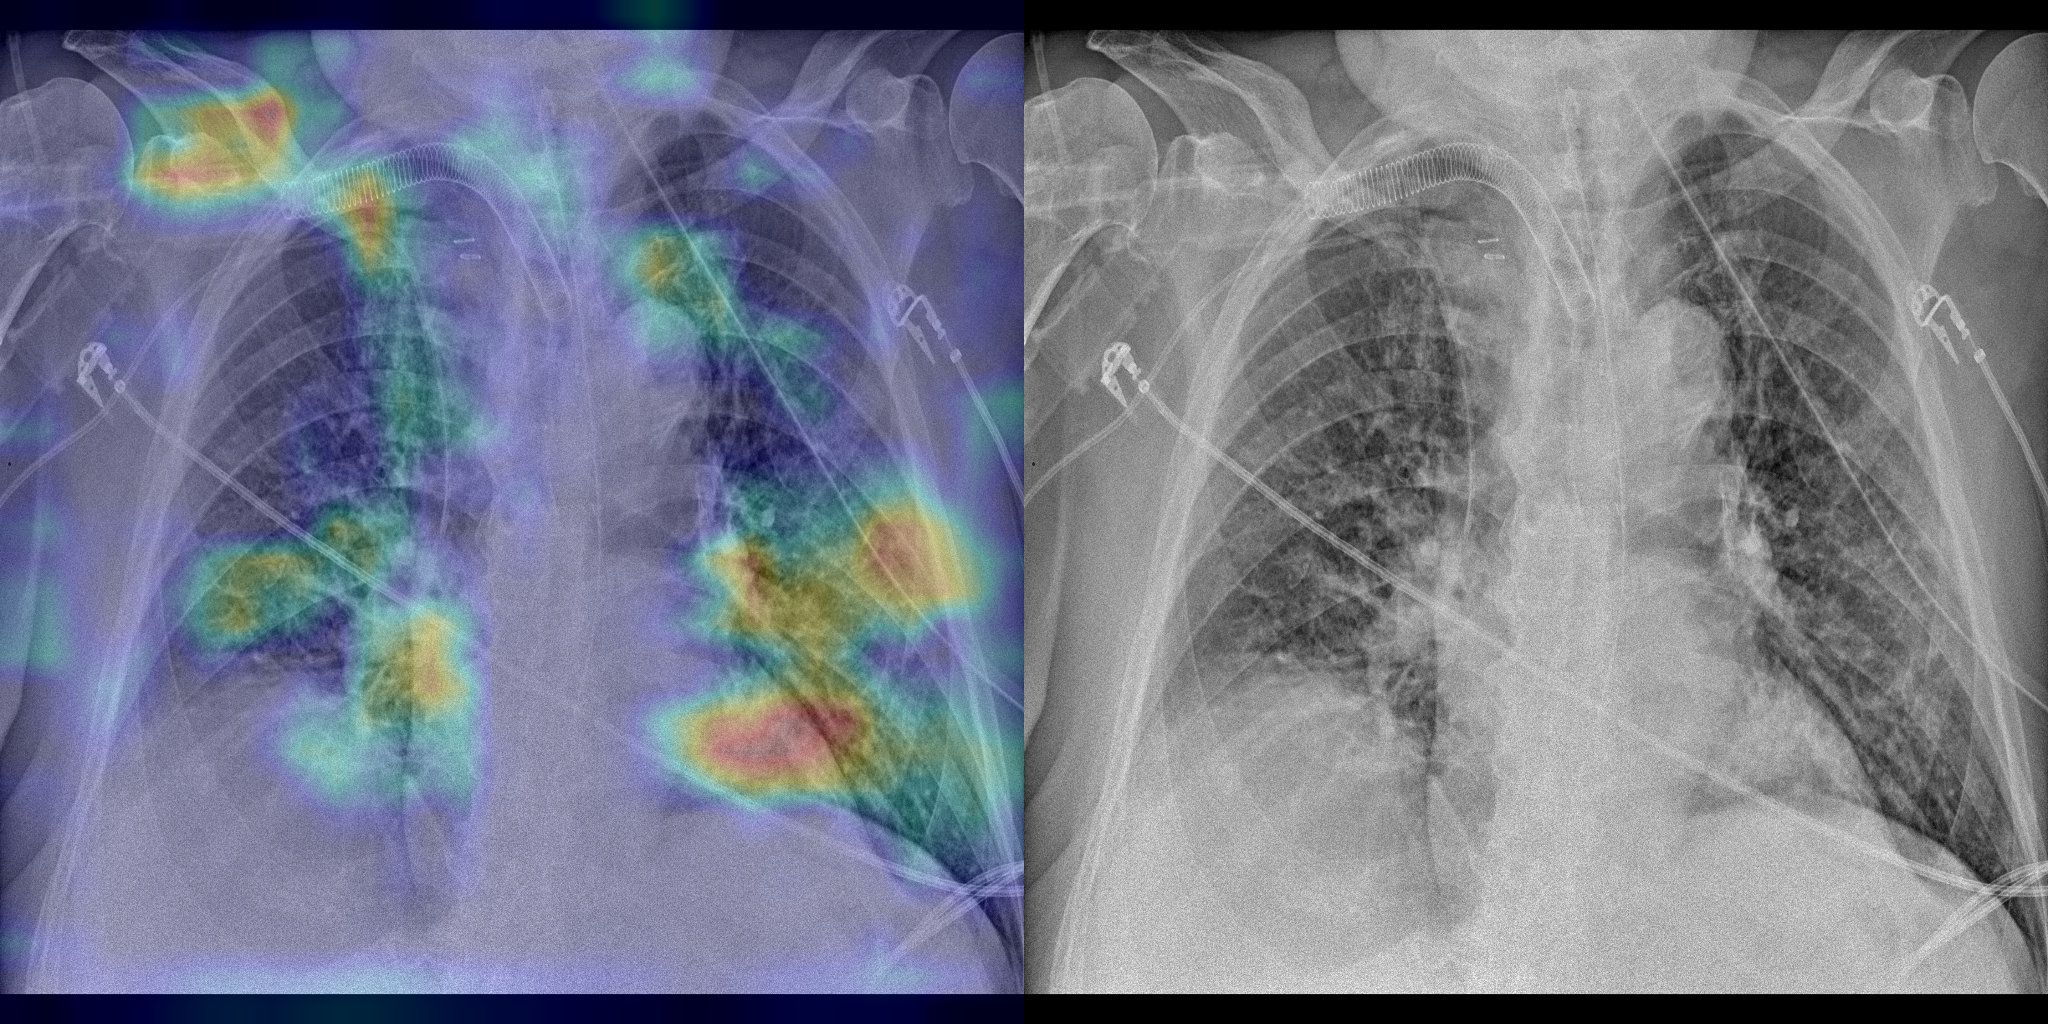
\includegraphics[width=1.0\textwidth]{Chapters/5. Conclusiones/img/COVID-19/1_1_1b5ca94ac38b_68fcf433c6fe.png}
    \end{subfigure}
    \begin{subfigure}{0.4\textwidth}
        \centering
        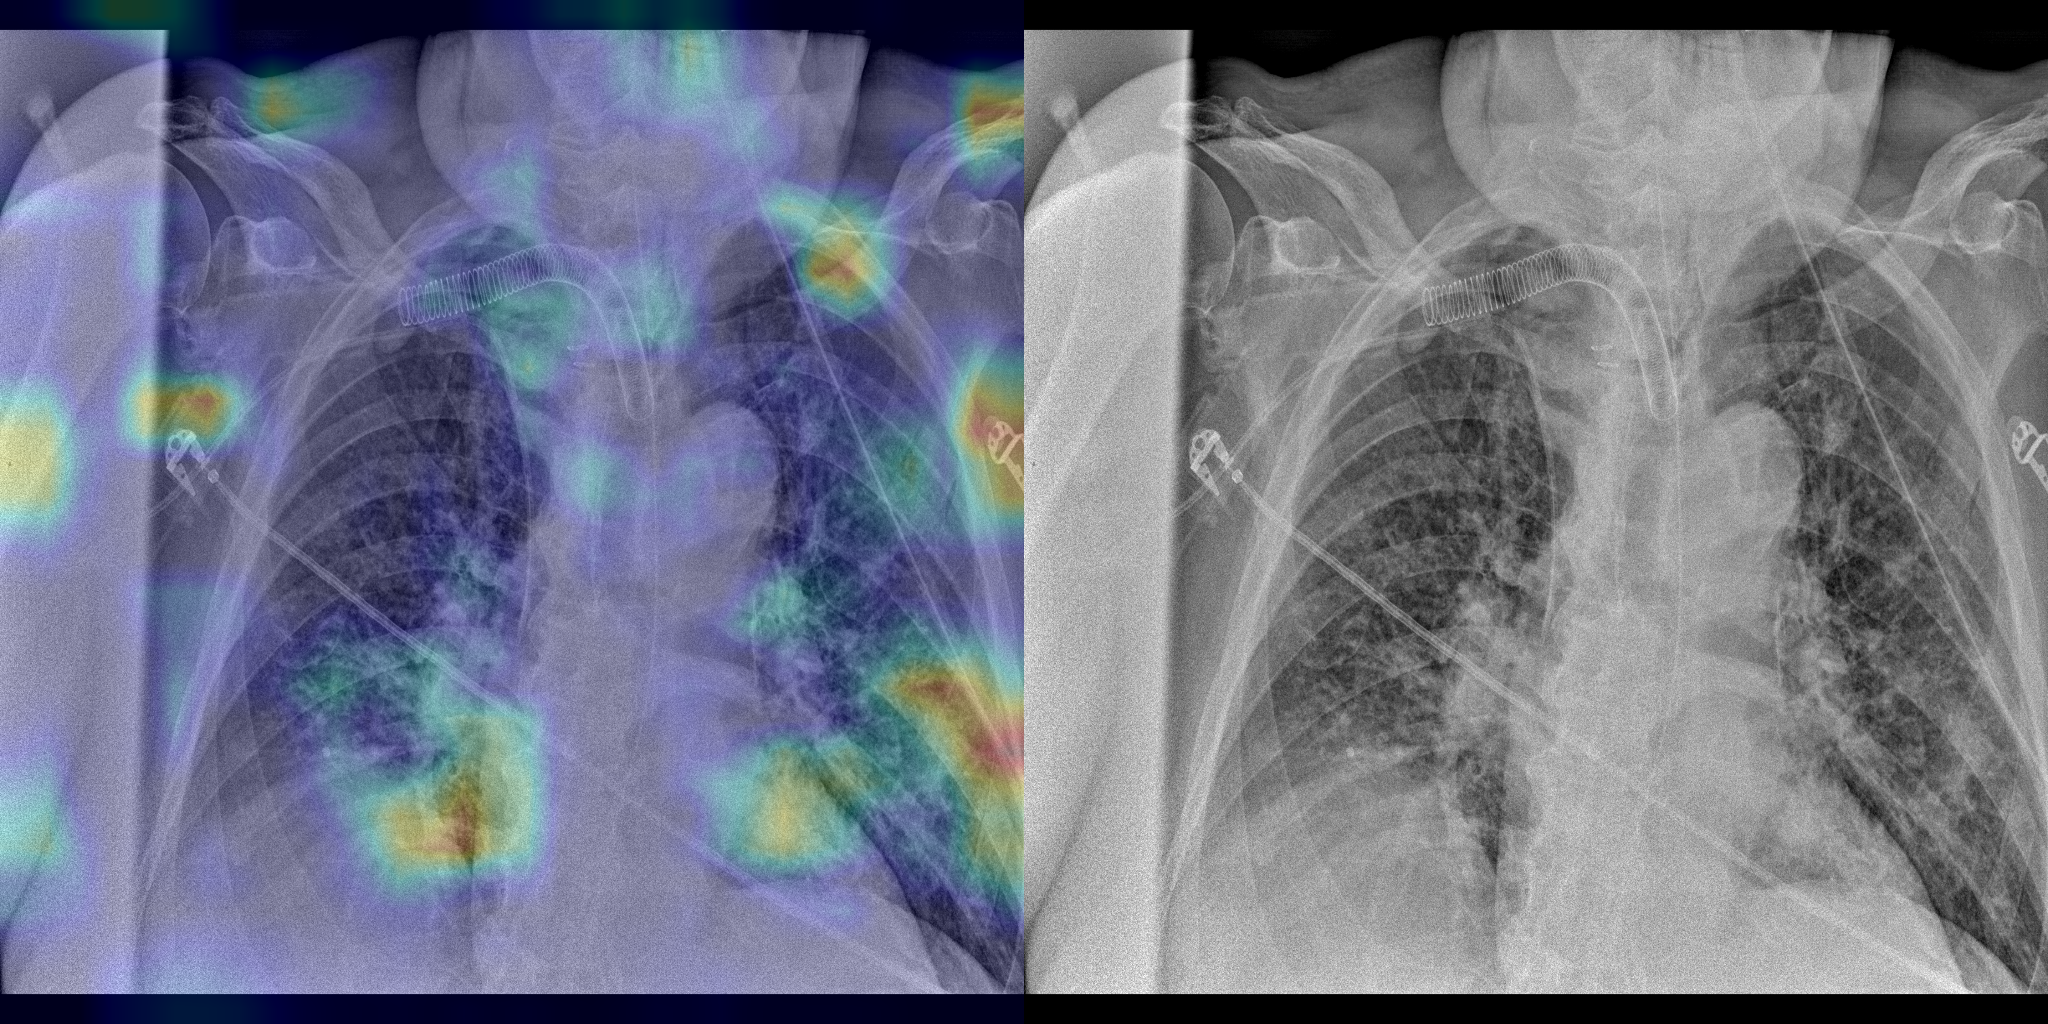
\includegraphics[width=1.0\textwidth]{Chapters/5. Conclusiones/img/COVID-19/1_1_1b5ca94ac38b_0919a3b8af01.png}
    \end{subfigure}
    \begin{subfigure}{0.4\textwidth}
        \centering
        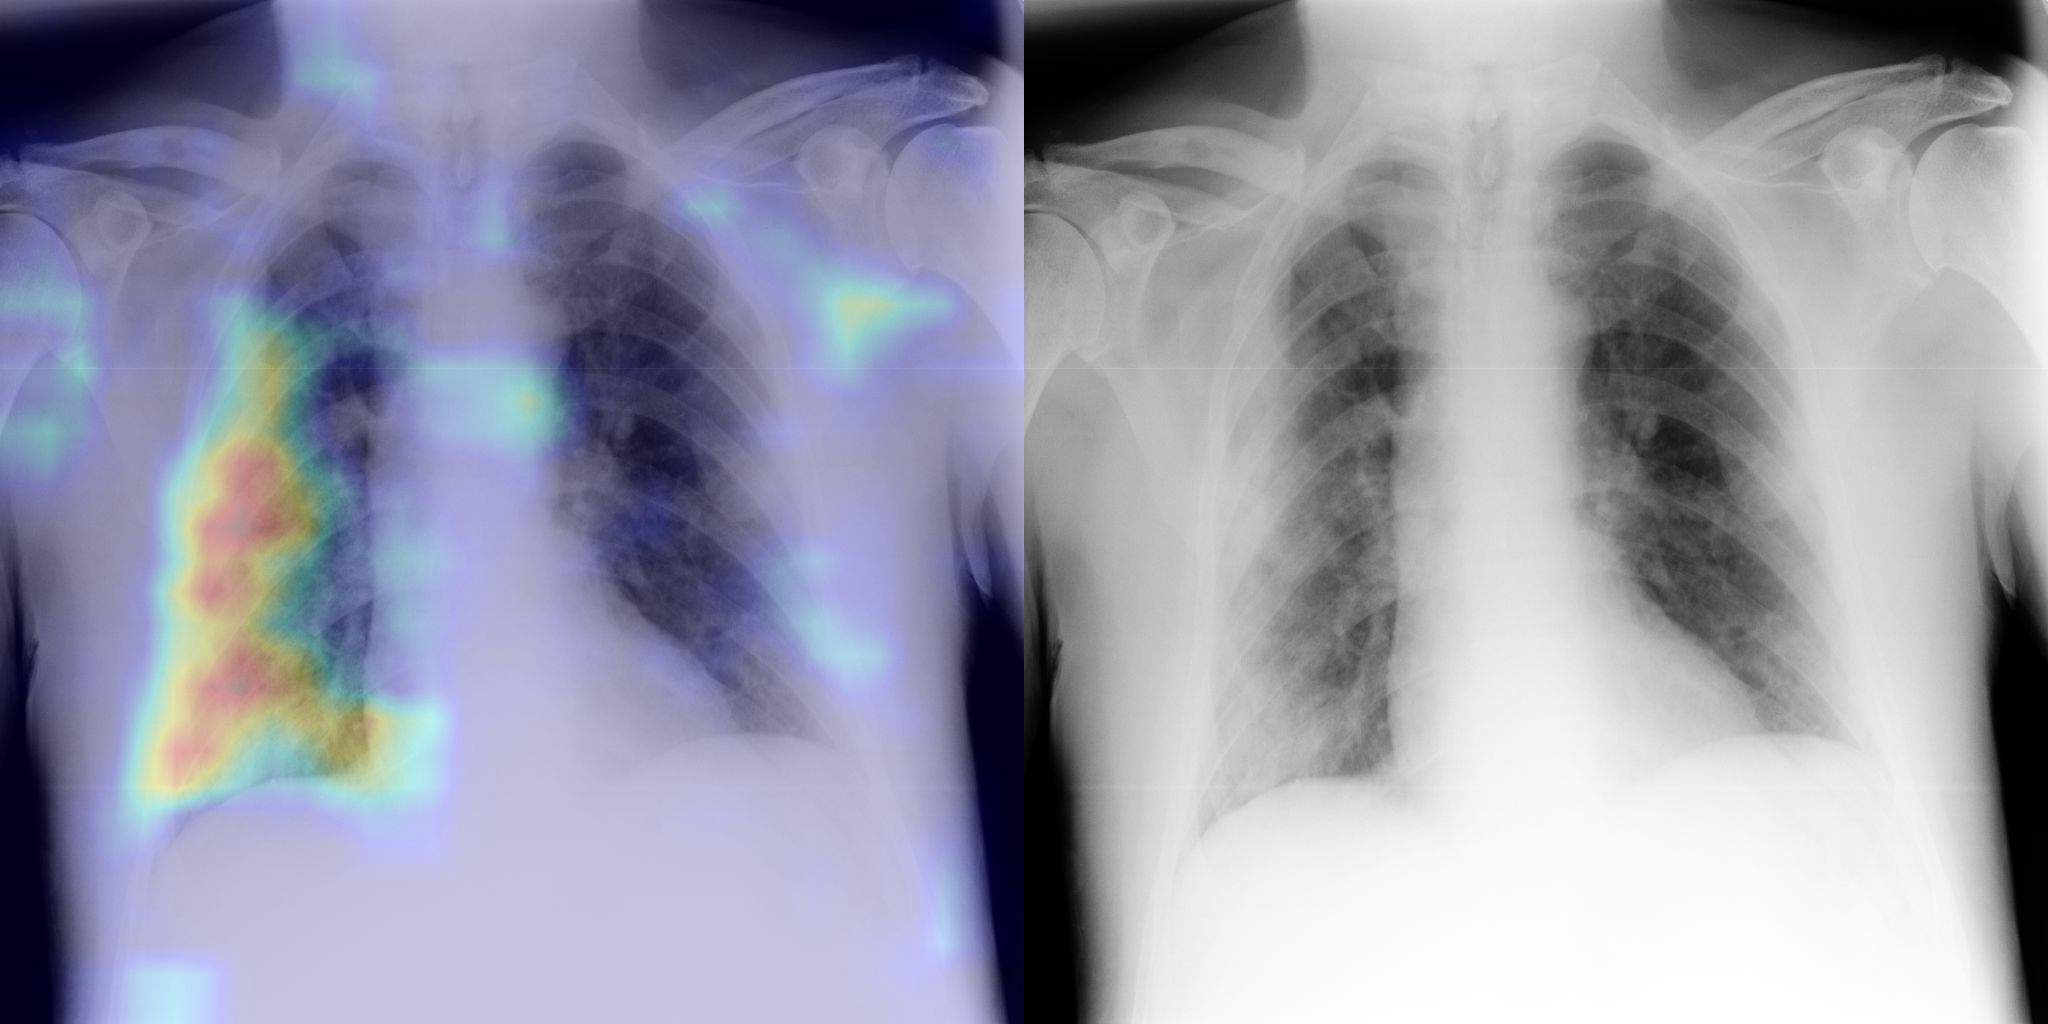
\includegraphics[width=1.0\textwidth]{Chapters/5. Conclusiones/img/COVID-19/1_1_1e3f6f8e494c_efe83e860c17.png}
    \end{subfigure}
    \begin{subfigure}{0.4\textwidth}
        \centering
        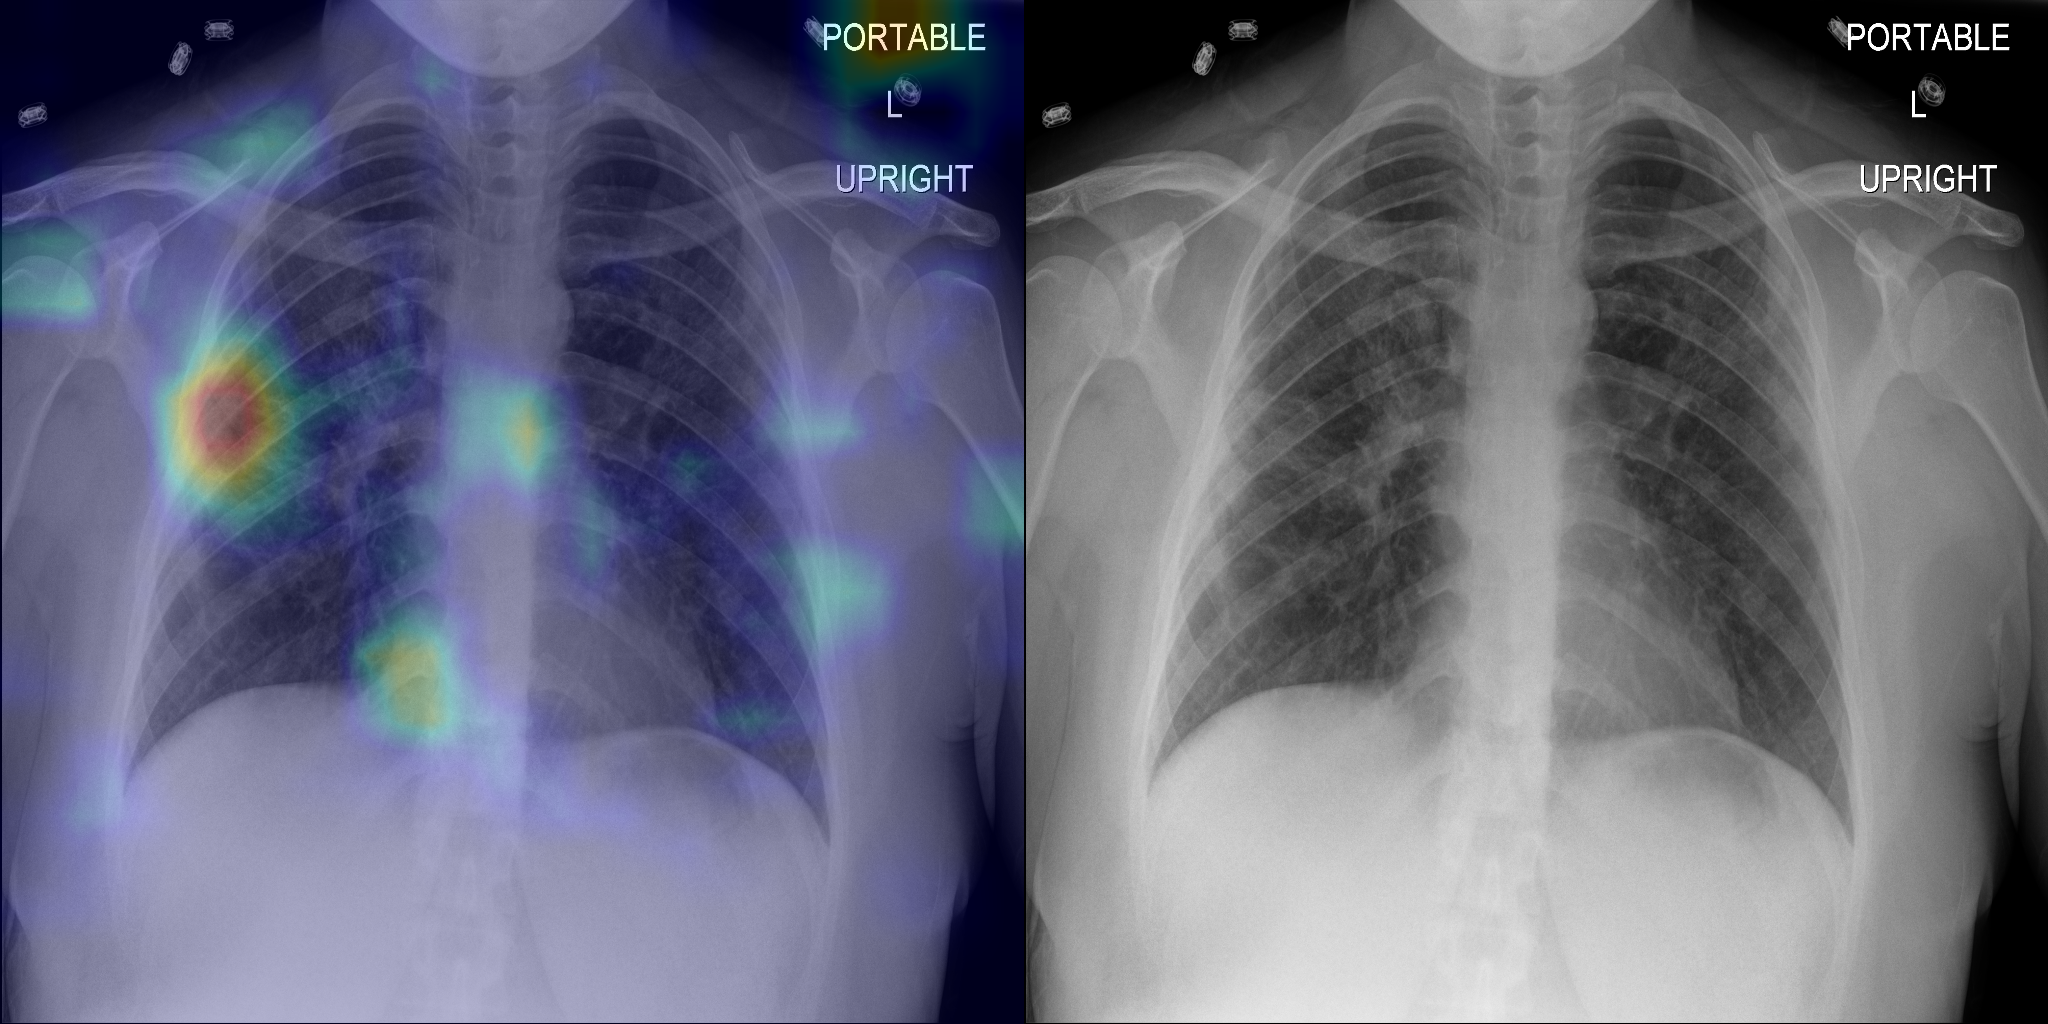
\includegraphics[width=1.0\textwidth]{Chapters/5. Conclusiones/img/COVID-19/1_1_4bb14a344446_0d3910133fbe.png}
    \end{subfigure}
    \begin{subfigure}{0.4\textwidth}
        \centering
        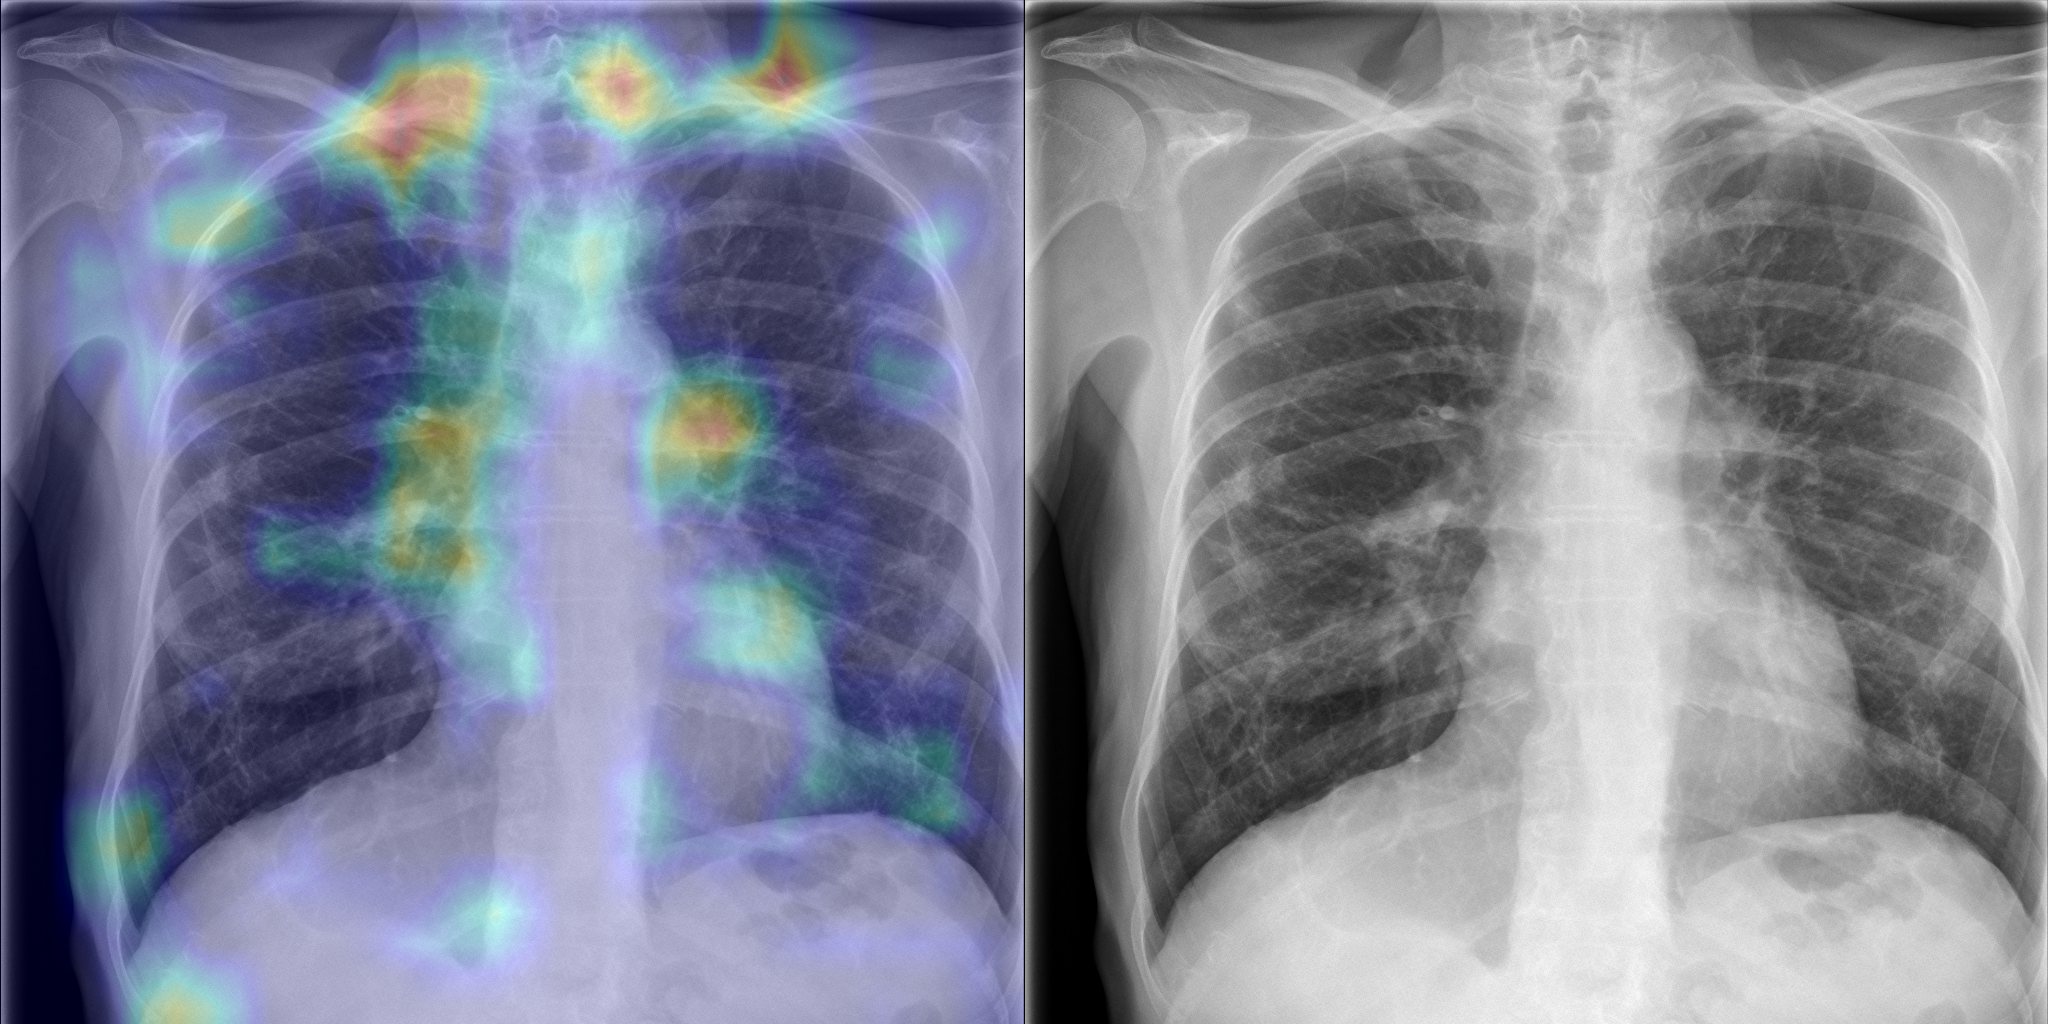
\includegraphics[width=1.0\textwidth]{Chapters/5. Conclusiones/img/COVID-19/1_1_4be426760e00_16d85c7f7837.png}
    \end{subfigure}
    \begin{subfigure}{0.4\textwidth}
        \centering
        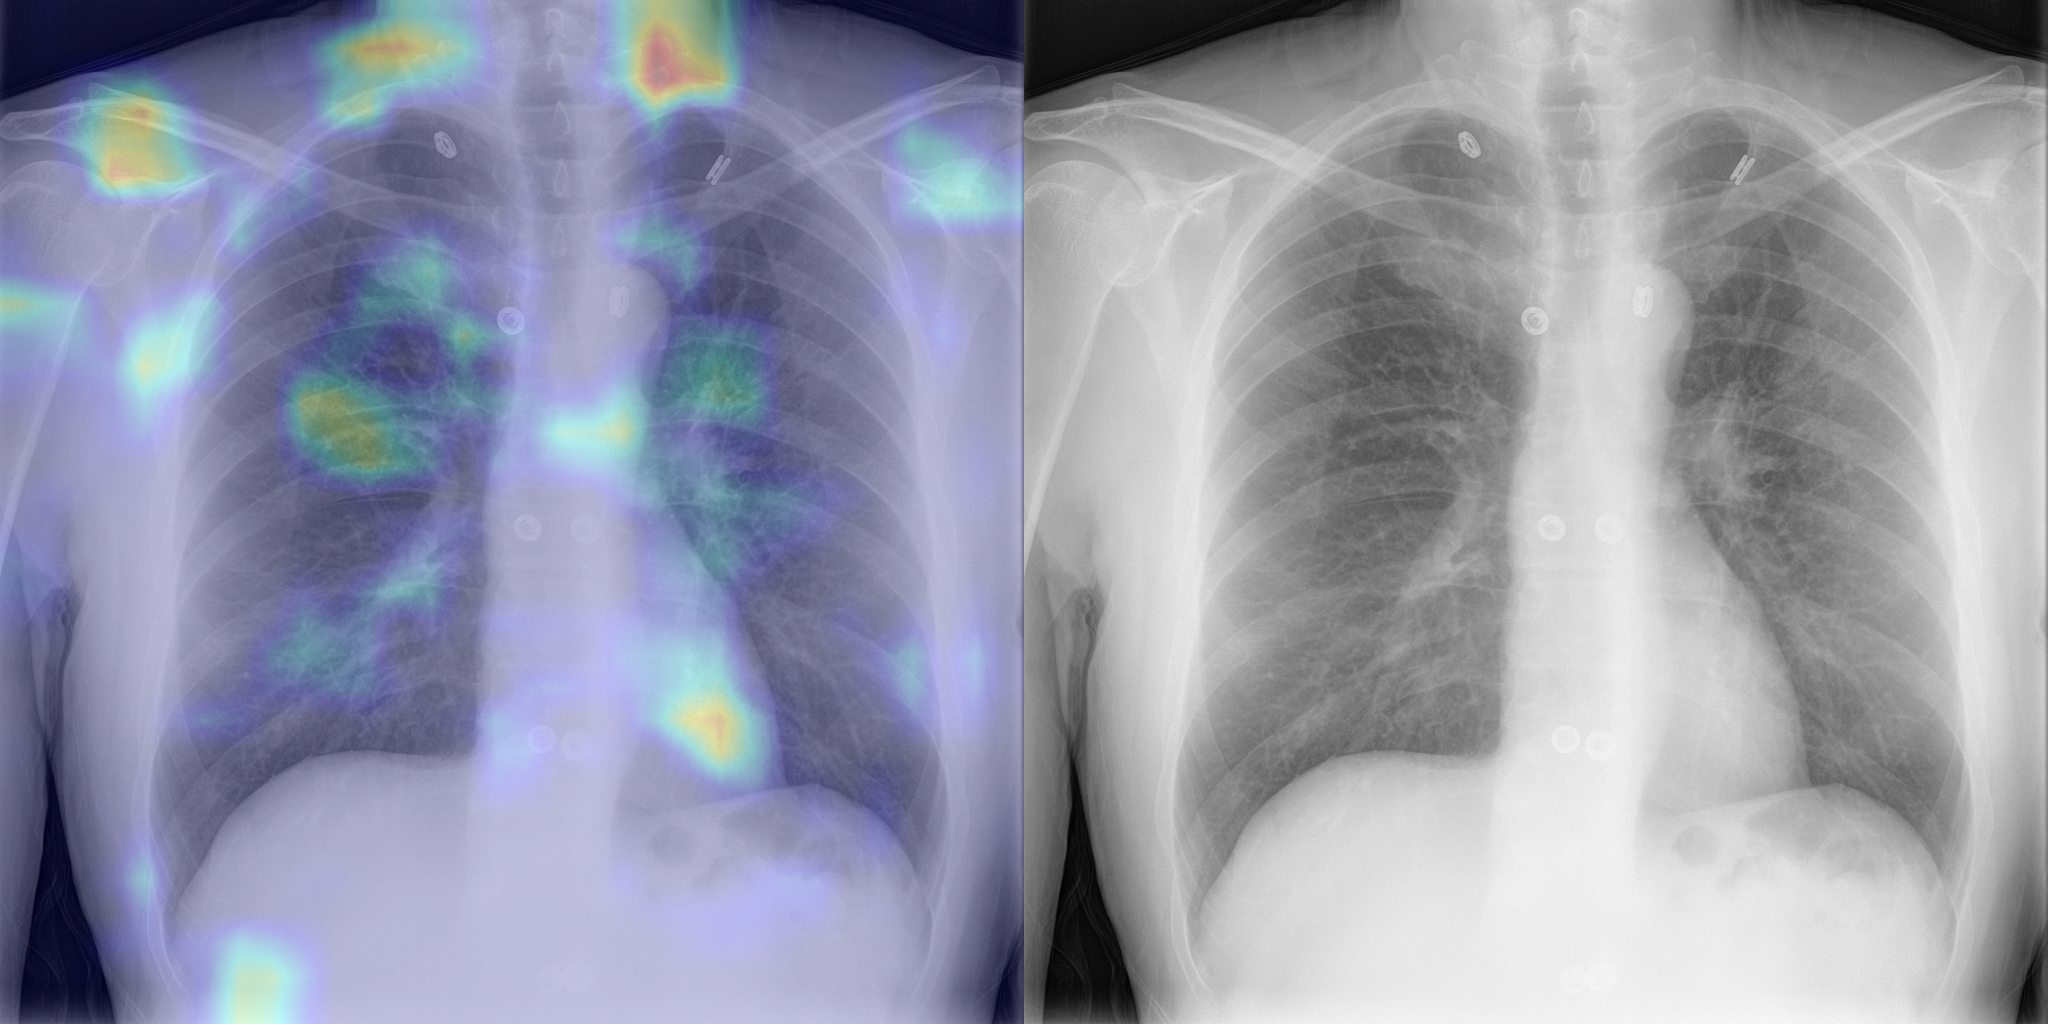
\includegraphics[width=1.0\textwidth]{Chapters/5. Conclusiones/img/COVID-19/1_1_7b6c49da06db_b6b631939d4f.png}
    \end{subfigure}
    \begin{subfigure}{0.4\textwidth}
        \centering
        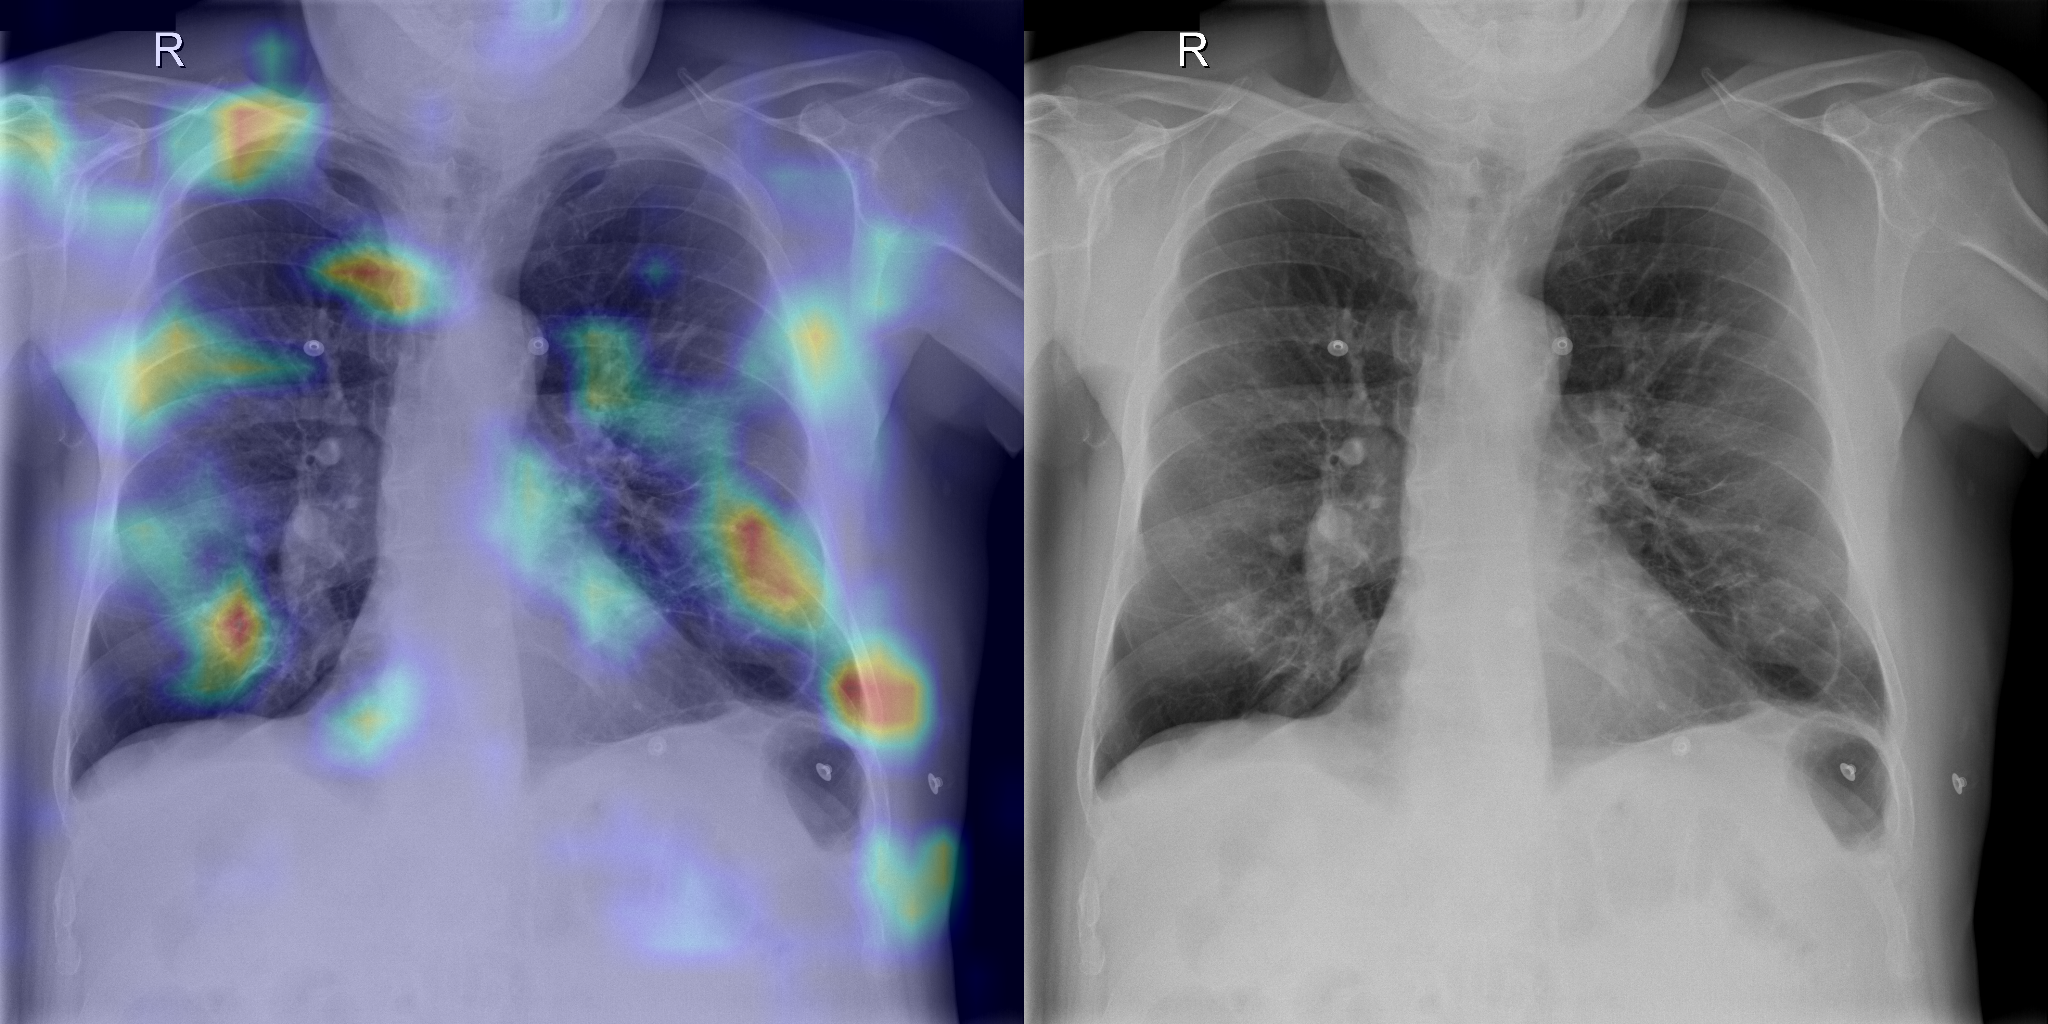
\includegraphics[width=1.0\textwidth]{Chapters/5. Conclusiones/img/COVID-19/1_1_cde0ab9526da_fa935d855d4e.png}
    \end{subfigure}
    \begin{subfigure}{0.4\textwidth}
        \centering
        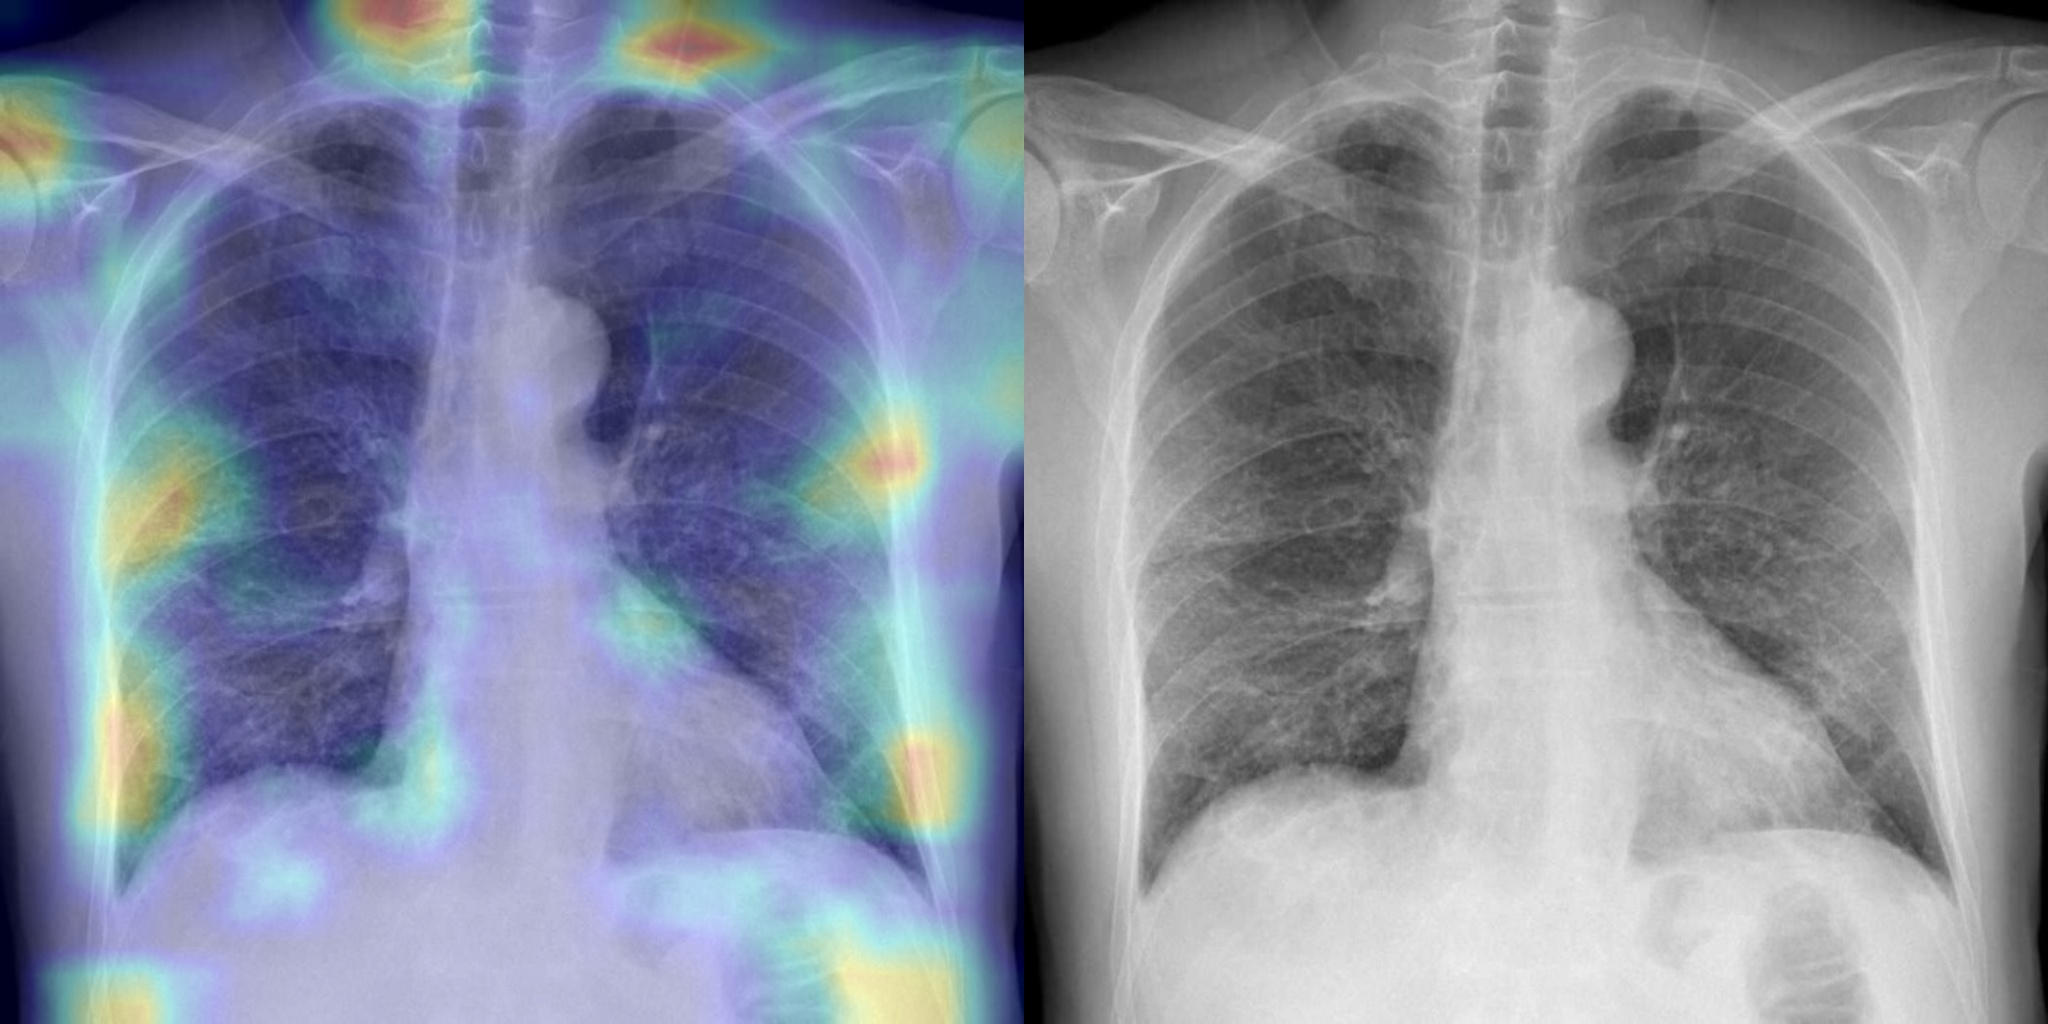
\includegraphics[width=1.0\textwidth]{Chapters/5. Conclusiones/img/COVID-19/1_1_covid-19-pneumonia-20-pa-on-admission.jpg}
    \end{subfigure}

    \caption{Covid-19. Radiografías detectadas con la patología de Covid-19 por los
                    radiólogos. A la izquierda de cada imagen el GradCam correspondiente a la detección
                    de la patología como positivo por el modelo CNN.}
\end{figure}

\begin{figure}[b]
    \centering
    \begin{subfigure}{0.4\textwidth}
        \centering
        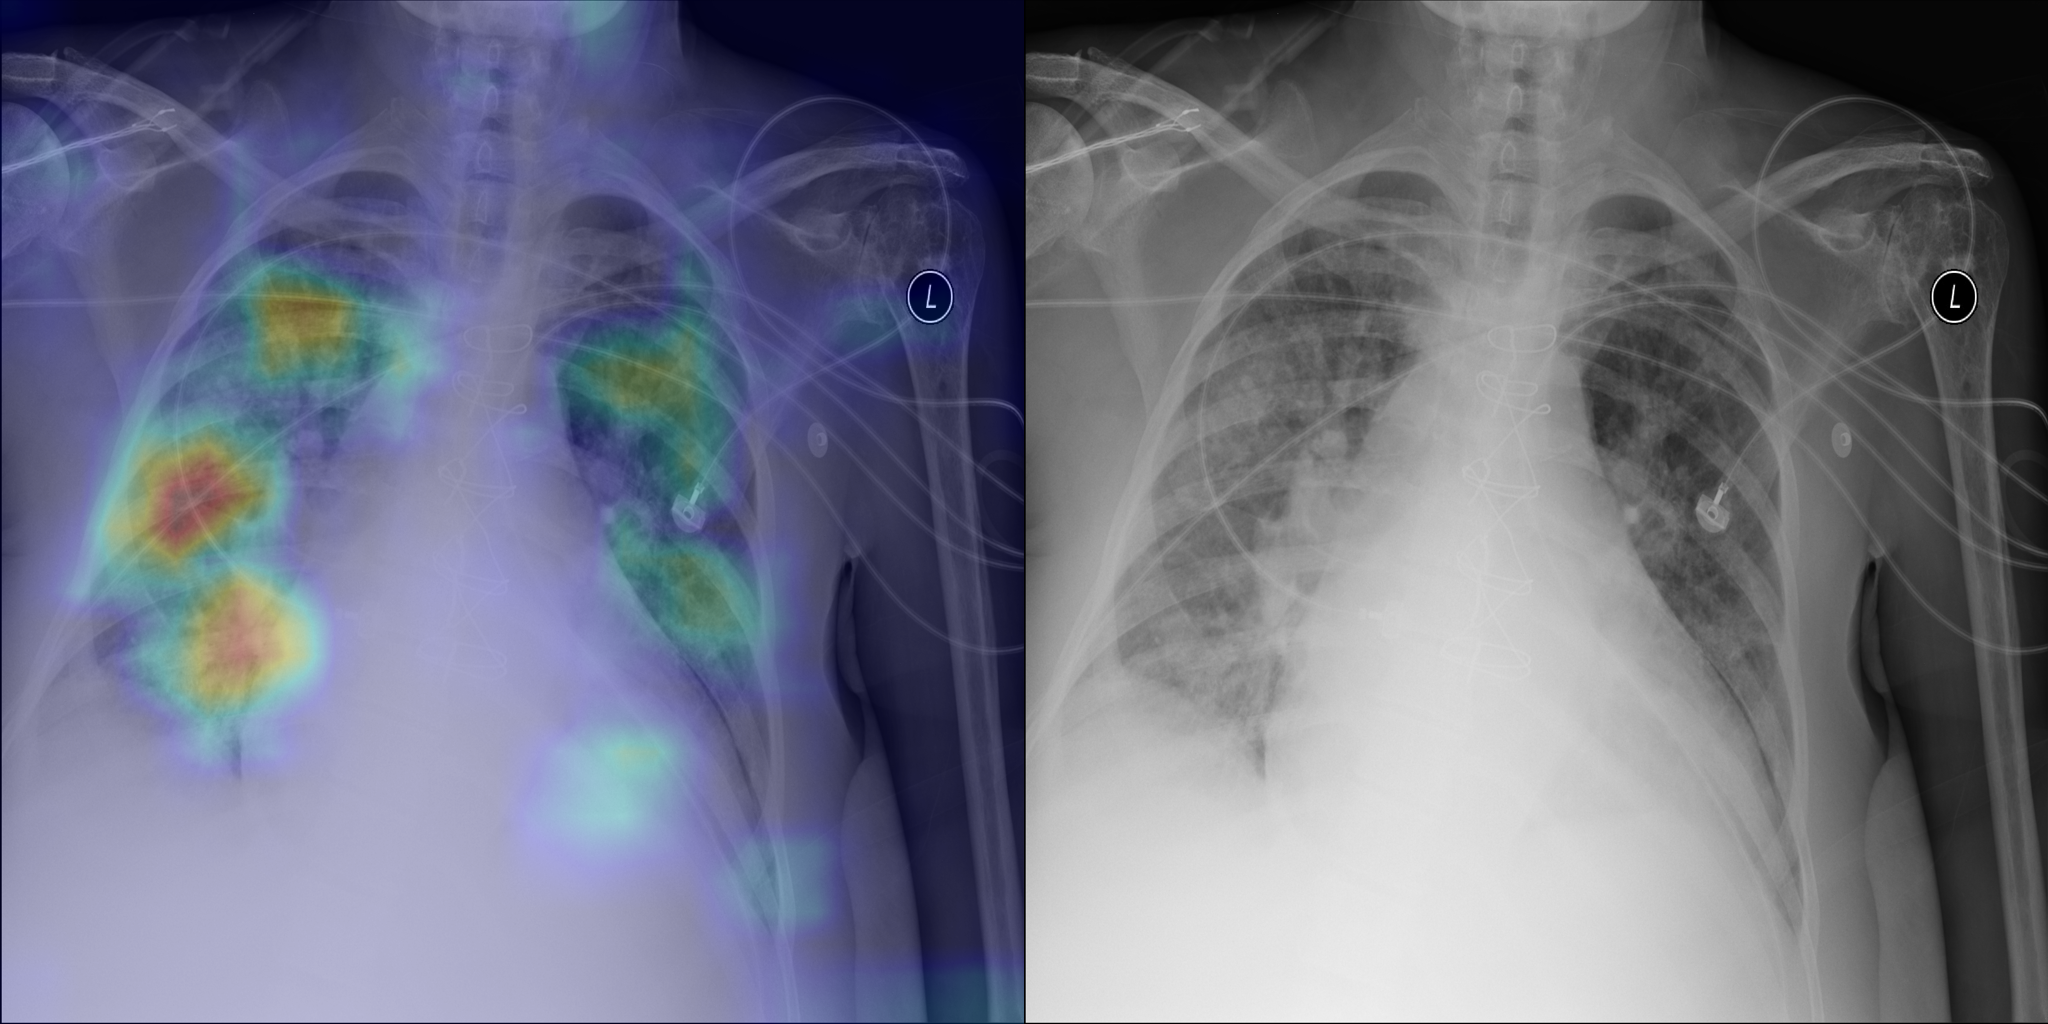
\includegraphics[width=1.0\textwidth]{Chapters/5. Conclusiones/img/Edema/1_1_00001373_031.png}
    \end{subfigure}
    \begin{subfigure}{0.4\textwidth}
        \centering
        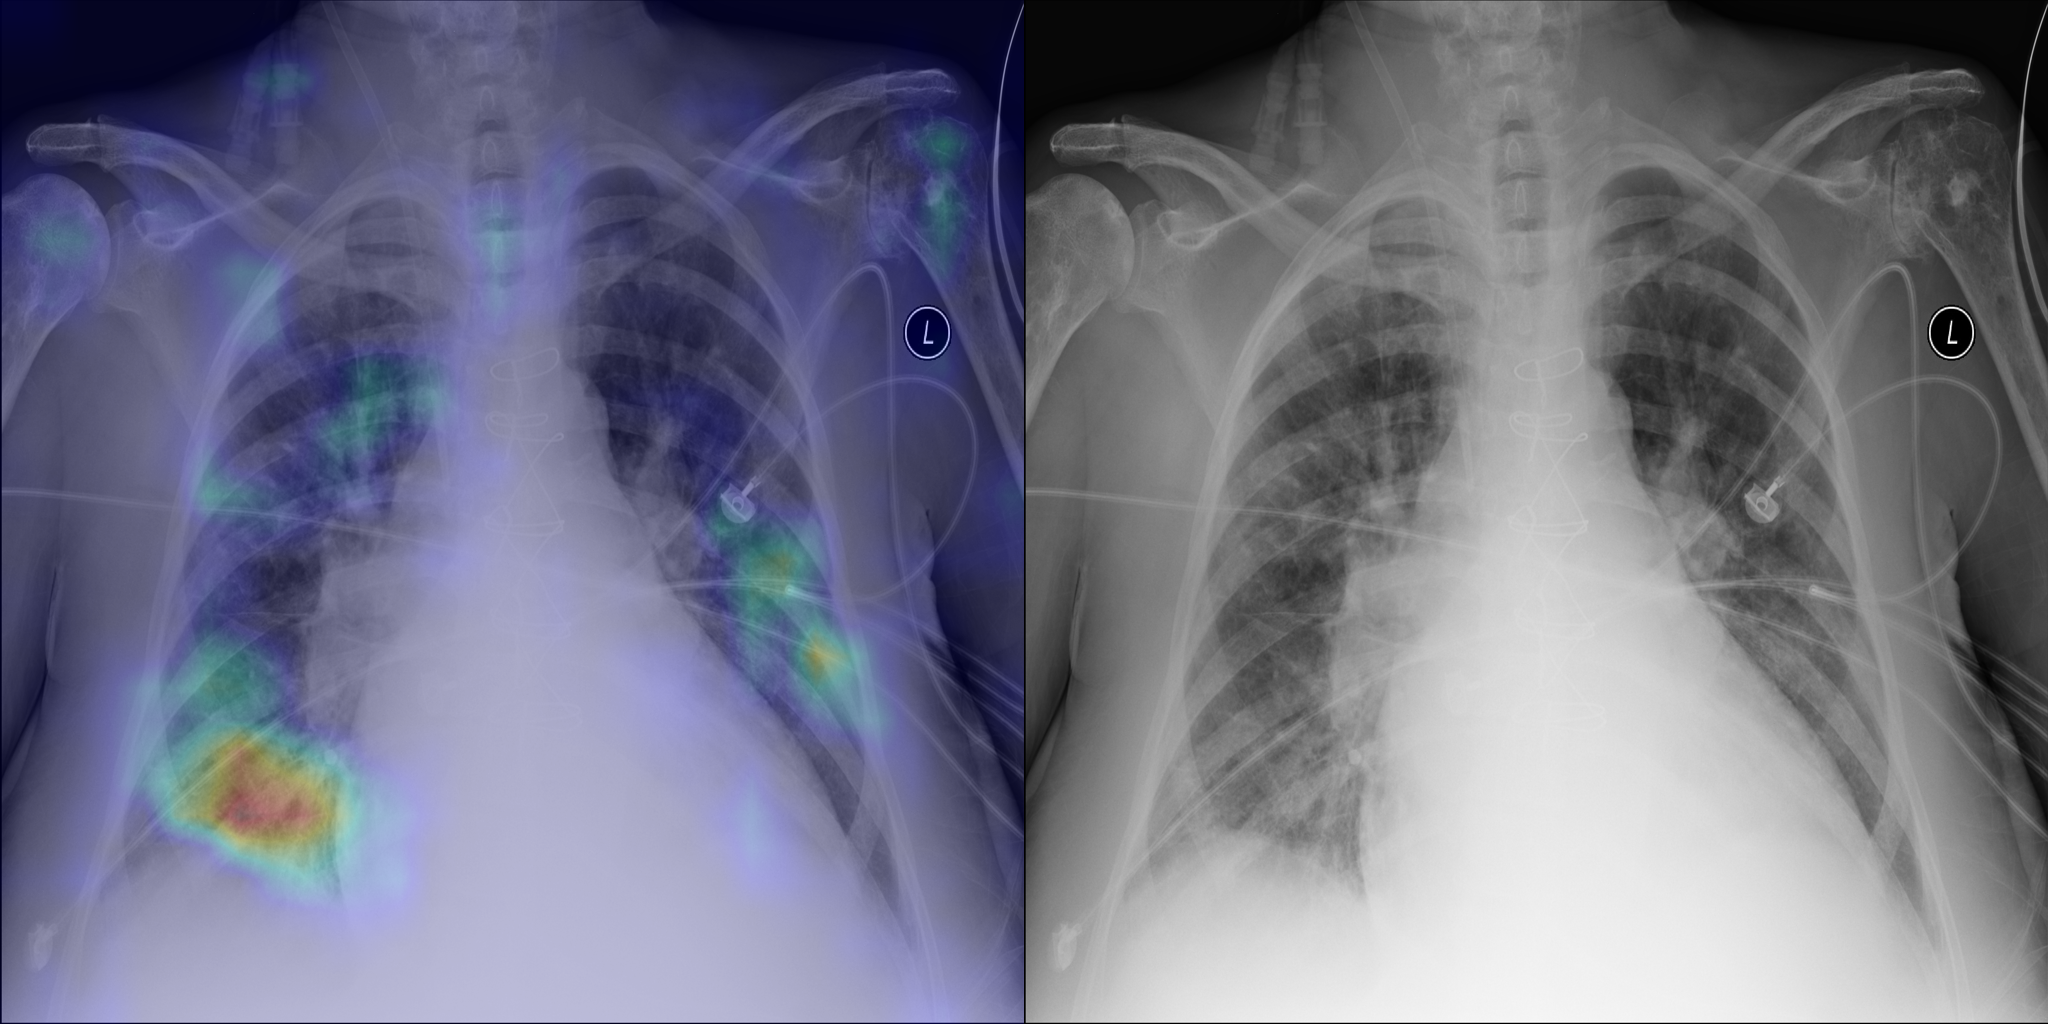
\includegraphics[width=1.0\textwidth]{Chapters/5. Conclusiones/img/Edema/1_1_00001373_032.png}
    \end{subfigure}
    \begin{subfigure}{0.4\textwidth}
        \centering
        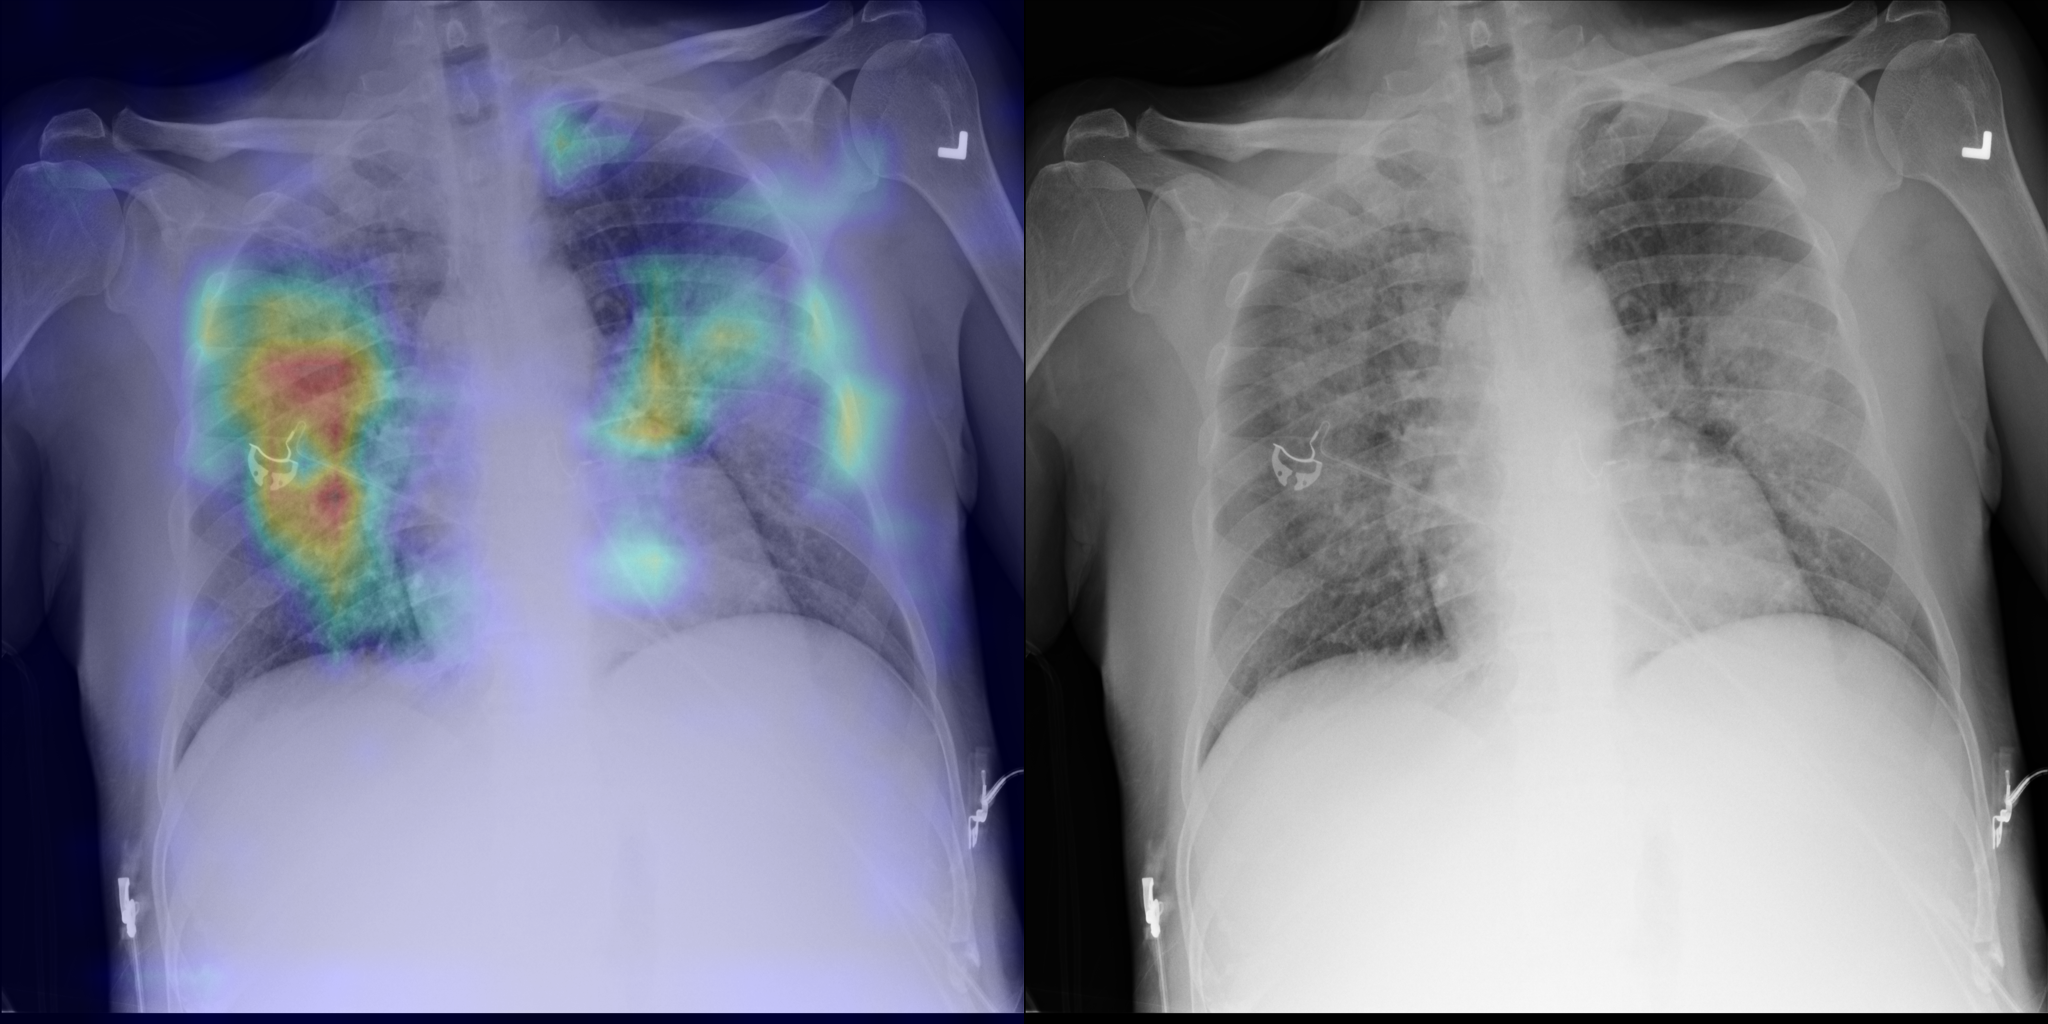
\includegraphics[width=1.0\textwidth]{Chapters/5. Conclusiones/img/Edema/1_1_00001787_000.png}
    \end{subfigure}
    \begin{subfigure}{0.4\textwidth}
        \centering
        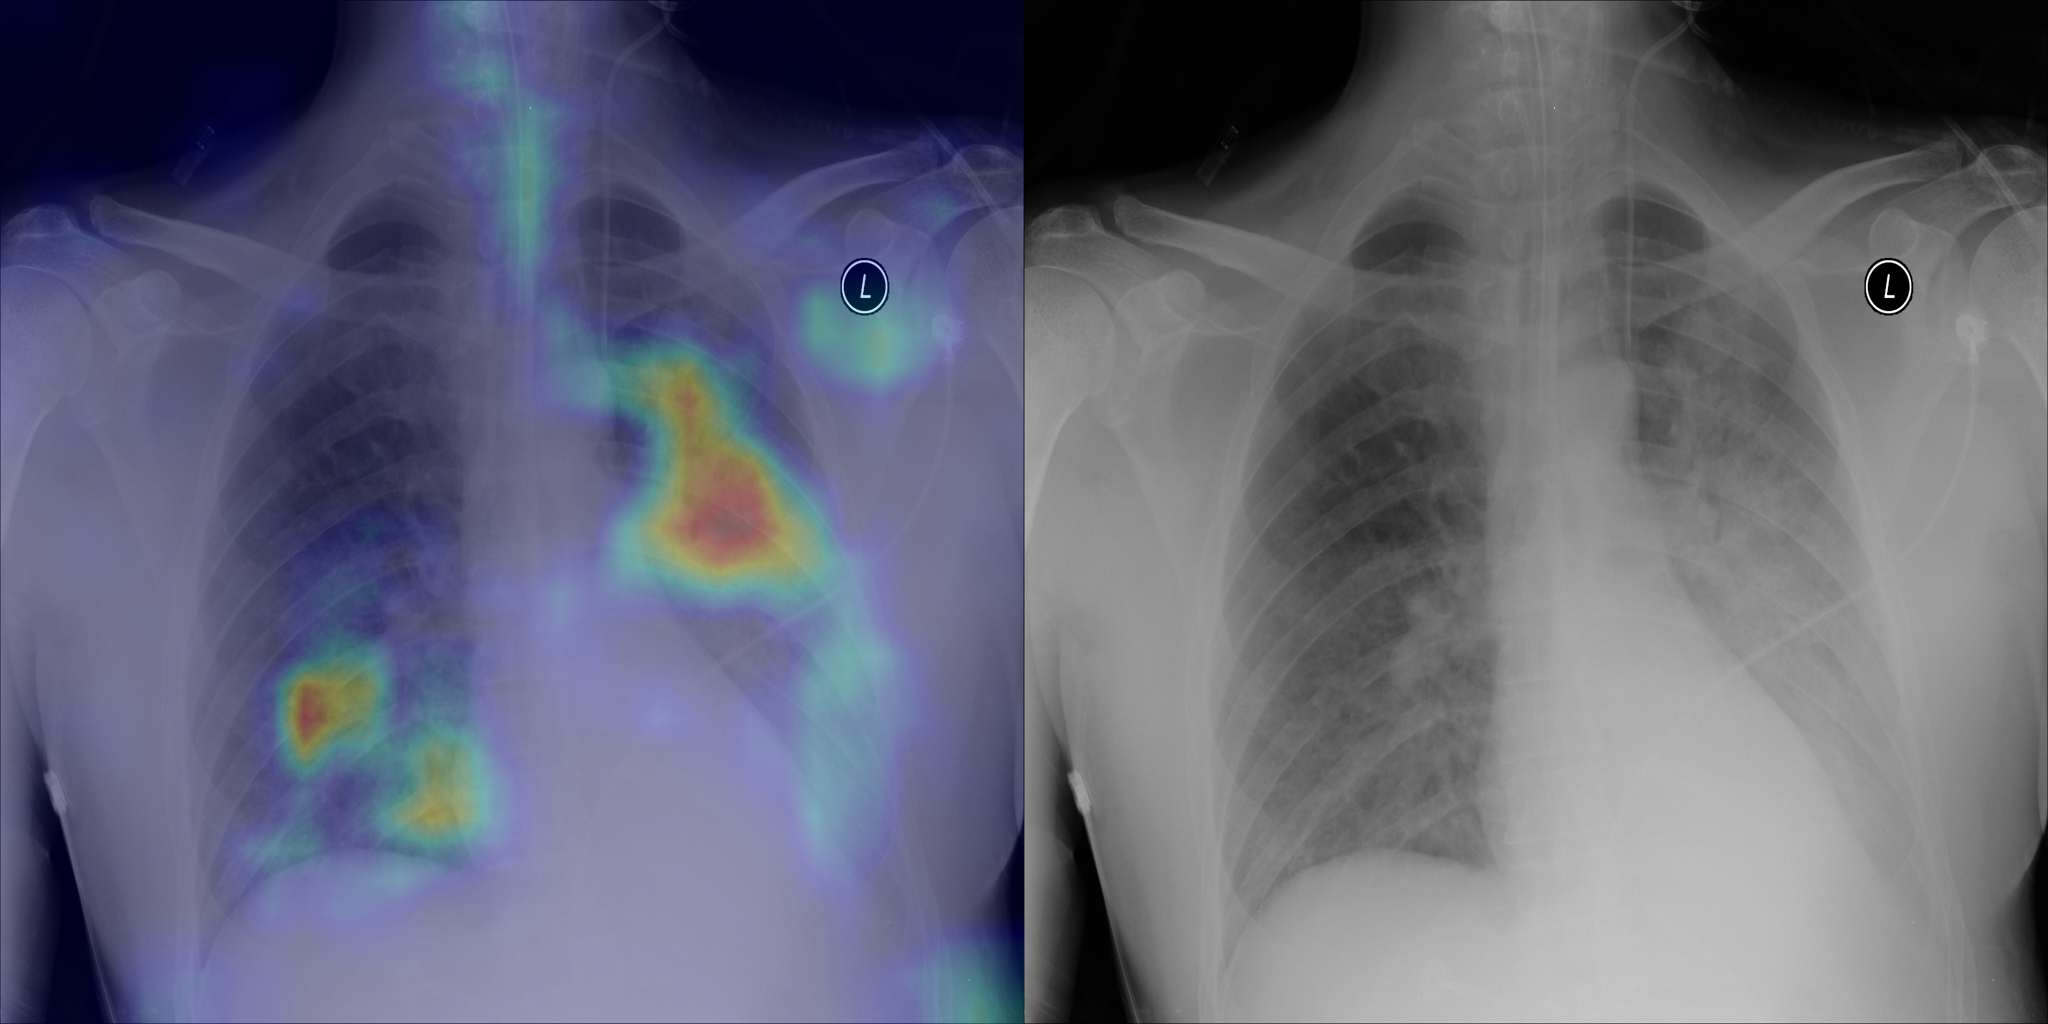
\includegraphics[width=1.0\textwidth]{Chapters/5. Conclusiones/img/Edema/1_1_00003528_021.png}
    \end{subfigure}
    \begin{subfigure}{0.4\textwidth}
        \centering
        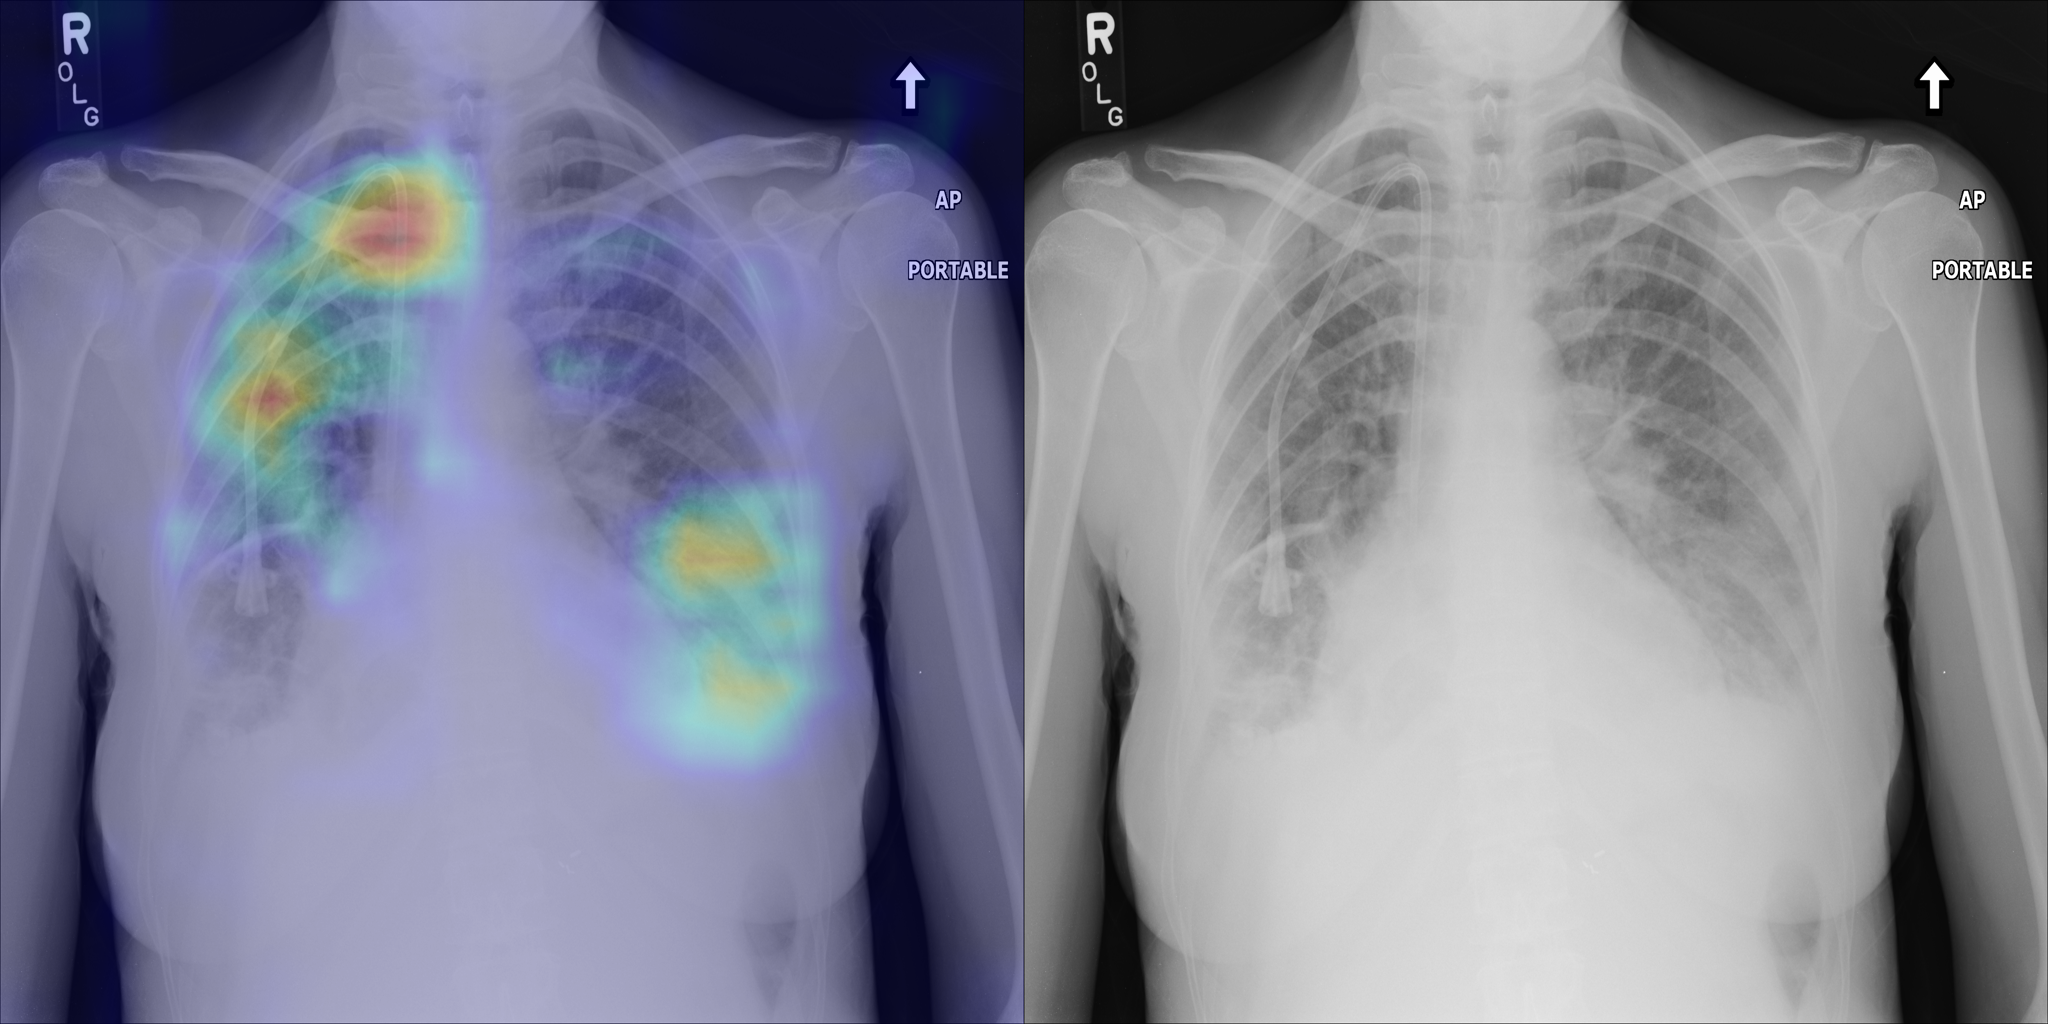
\includegraphics[width=1.0\textwidth]{Chapters/5. Conclusiones/img/Edema/1_1_00003803_009.png}
    \end{subfigure}
    \begin{subfigure}{0.4\textwidth}
        \centering
        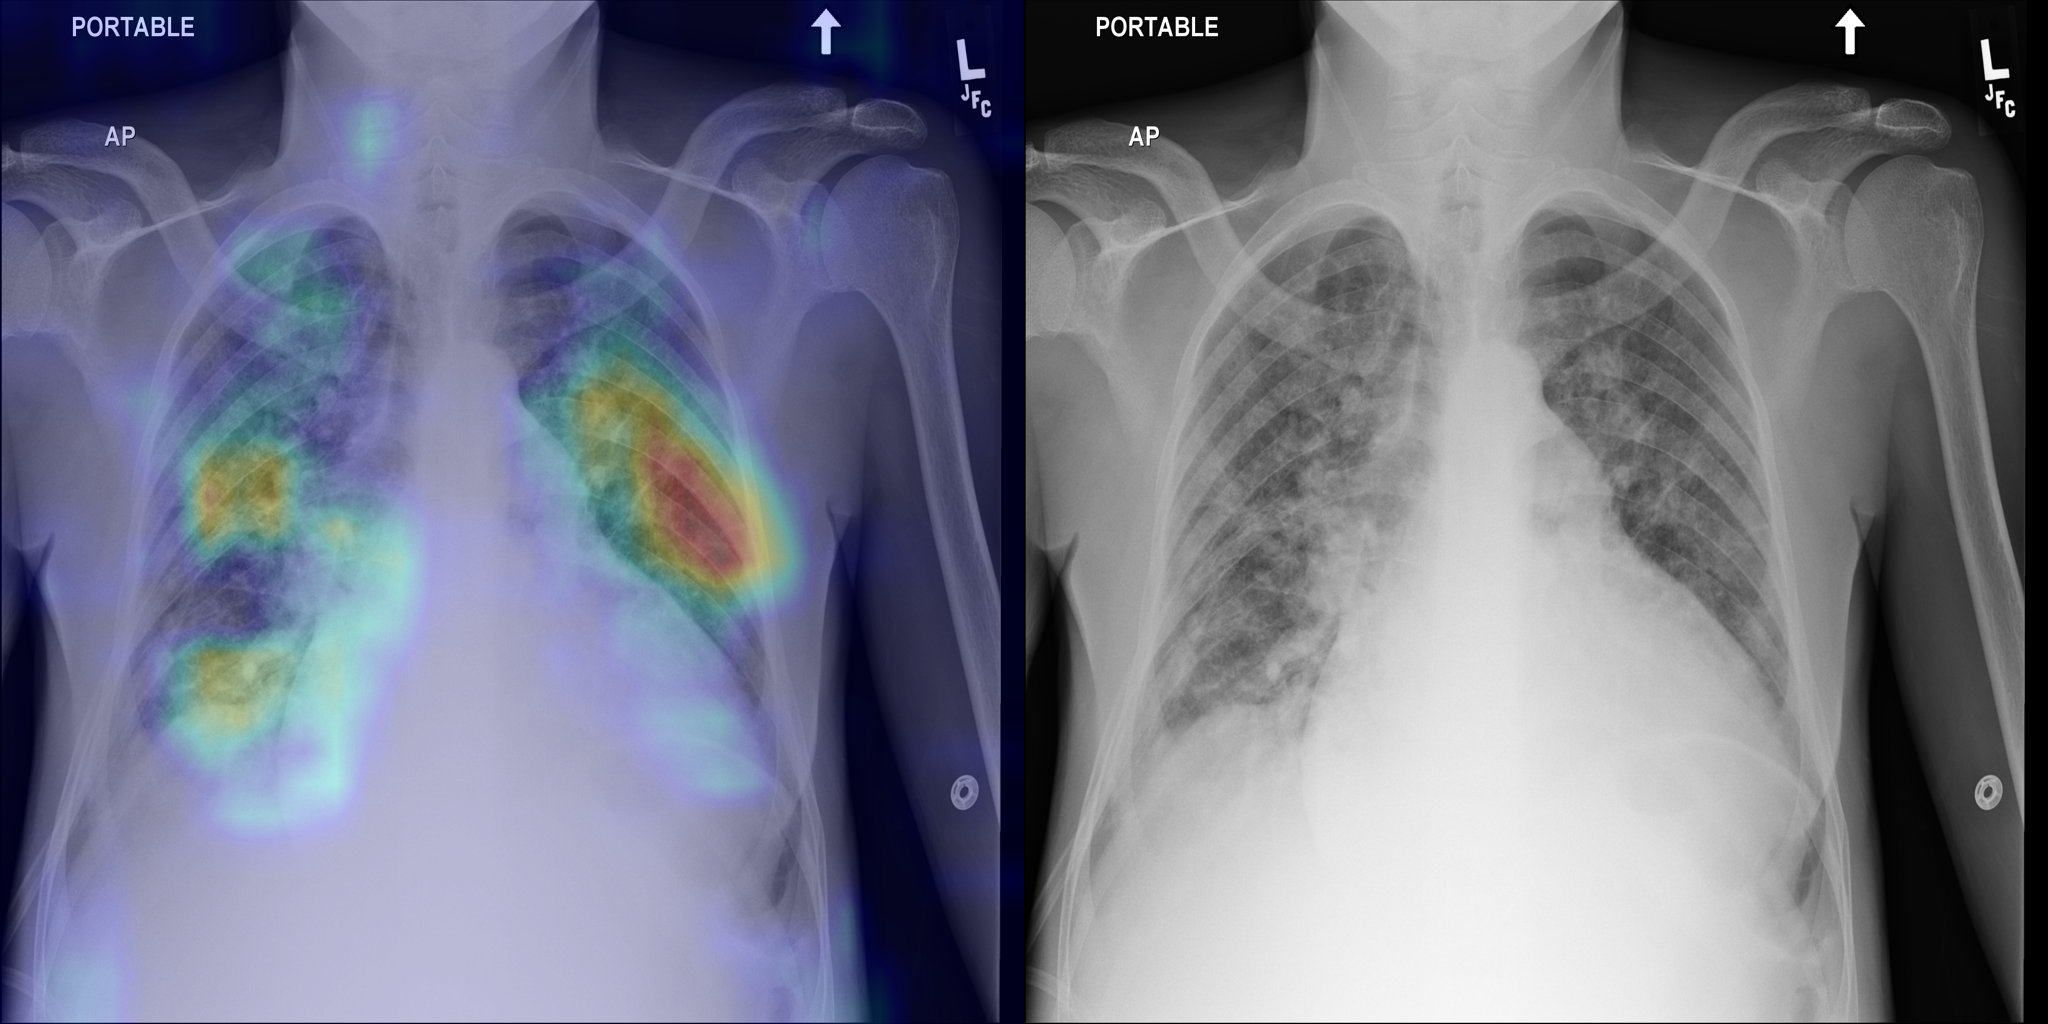
\includegraphics[width=1.0\textwidth]{Chapters/5. Conclusiones/img/Edema/1_1_00004533_020.png}
    \end{subfigure}
    \begin{subfigure}{0.4\textwidth}
        \centering
        \includegraphics[width=1.0\textwidth]{Chapters/5. Conclusiones/img/Edema/1_1_00006304_002.png}
    \end{subfigure}
    \begin{subfigure}{0.4\textwidth}
        \centering
        \includegraphics[width=1.0\textwidth]{Chapters/5. Conclusiones/img/Edema/1_1_00006304_006.png}
    \end{subfigure}
    \begin{subfigure}{0.4\textwidth}
        \centering
        \includegraphics[width=1.0\textwidth]{Chapters/5. Conclusiones/img/Edema/1_1_00010535_002.png}
    \end{subfigure}
    \begin{subfigure}{0.4\textwidth}
        \centering
        \includegraphics[width=1.0\textwidth]{Chapters/5. Conclusiones/img/Edema/1_1_00011583_006.png}
    \end{subfigure}

    \caption{Edema. Radiografías detectadas con la patología de edema pulmonar por los
                    radiólogos. A la izquierda de cada imagen el GradCam correspondiente a la detección
                    de la patología como positivo por el modelo CNN.}
\end{figure}

\begin{figure}[b]
    \centering
    \begin{subfigure}{0.4\textwidth}
        \centering
        \includegraphics[width=1.0\textwidth]{Chapters/5. Conclusiones/img/Effusion/1_1_00000092_001.png}
    \end{subfigure}
    \begin{subfigure}{0.4\textwidth}
        \centering
        \includegraphics[width=1.0\textwidth]{Chapters/5. Conclusiones/img/Effusion/1_1_00000147_002.png}
    \end{subfigure}
    \begin{subfigure}{0.4\textwidth}
        \centering
        \includegraphics[width=1.0\textwidth]{Chapters/5. Conclusiones/img/Effusion/1_1_00000181_005.png}
    \end{subfigure}
    \begin{subfigure}{0.4\textwidth}
        \centering
        \includegraphics[width=1.0\textwidth]{Chapters/5. Conclusiones/img/Effusion/1_1_00000181_054.png}
    \end{subfigure}
    \begin{subfigure}{0.4\textwidth}
        \centering
        \includegraphics[width=1.0\textwidth]{Chapters/5. Conclusiones/img/Effusion/1_1_00000181_055.png}
    \end{subfigure}
    \begin{subfigure}{0.4\textwidth}
        \centering
        \includegraphics[width=1.0\textwidth]{Chapters/5. Conclusiones/img/Effusion/1_1_00000211_004.png}
    \end{subfigure}
    \begin{subfigure}{0.4\textwidth}
        \centering
        \includegraphics[width=1.0\textwidth]{Chapters/5. Conclusiones/img/Effusion/1_1_00000211_008.png}
    \end{subfigure}
    \begin{subfigure}{0.4\textwidth}
        \centering
        \includegraphics[width=1.0\textwidth]{Chapters/5. Conclusiones/img/Effusion/1_1_00000211_011.png}
    \end{subfigure}
    \begin{subfigure}{0.4\textwidth}
        \centering
        \includegraphics[width=1.0\textwidth]{Chapters/5. Conclusiones/img/Effusion/1_1_00022883_011.png}
    \end{subfigure}
    \begin{subfigure}{0.4\textwidth}
        \centering
        \includegraphics[width=1.0\textwidth]{Chapters/5. Conclusiones/img/Effusion/1_1_00022899_009.png}
    \end{subfigure}

    \caption{Derrame pleural. Radiografías detectadas con la patología de derrame pleural por los
                    radiólogos. A la izquierda de cada imagen el GradCam correspondiente a la detección
                    de la patología como positivo por el modelo CNN.}
\end{figure}

\begin{figure}[b]
    \centering
    \begin{subfigure}{0.4\textwidth}
        \centering
        \includegraphics[width=1.0\textwidth]{Chapters/5. Conclusiones/img/Emphysema/1_1_00000312_001.png}
    \end{subfigure}
    \begin{subfigure}{0.4\textwidth}
        \centering
        \includegraphics[width=1.0\textwidth]{Chapters/5. Conclusiones/img/Emphysema/1_1_00000732_006.png}
    \end{subfigure}
    \begin{subfigure}{0.4\textwidth}
        \centering
        \includegraphics[width=1.0\textwidth]{Chapters/5. Conclusiones/img/Emphysema/1_1_00001093_000.png}
    \end{subfigure}
    \begin{subfigure}{0.4\textwidth}
        \centering
        \includegraphics[width=1.0\textwidth]{Chapters/5. Conclusiones/img/Emphysema/1_1_00001555_000.png}
    \end{subfigure}
    \begin{subfigure}{0.4\textwidth}
        \centering
        \includegraphics[width=1.0\textwidth]{Chapters/5. Conclusiones/img/Emphysema/1_1_00008841_062.png}
    \end{subfigure}
    \begin{subfigure}{0.4\textwidth}
        \centering
        \includegraphics[width=1.0\textwidth]{Chapters/5. Conclusiones/img/Emphysema/1_1_00011683_042.png}
    \end{subfigure}
    \begin{subfigure}{0.4\textwidth}
        \centering
        \includegraphics[width=1.0\textwidth]{Chapters/5. Conclusiones/img/Emphysema/1_1_00012298_007.png}
    \end{subfigure}
    \begin{subfigure}{0.4\textwidth}
        \centering
        \includegraphics[width=1.0\textwidth]{Chapters/5. Conclusiones/img/Emphysema/1_1_00015387_000.png}
    \end{subfigure}
    \begin{subfigure}{0.4\textwidth}
        \centering
        \includegraphics[width=1.0\textwidth]{Chapters/5. Conclusiones/img/Emphysema/1_1_00023075_007.png}
    \end{subfigure}
    \begin{subfigure}{0.4\textwidth}
        \centering
        \includegraphics[width=1.0\textwidth]{Chapters/5. Conclusiones/img/Emphysema/1_1_00023078_006.png}
    \end{subfigure}

    \caption{Enfisema pulmonar. Radiografías detectadas con la patología de enfisema pulmonar por los
                    radiólogos. A la izquierda de cada imagen el GradCam correspondiente a la detección
                    de la patología como positivo por el modelo CNN.}
\end{figure}

\begin{figure}[b]
    \centering
    \begin{subfigure}{0.4\textwidth}
        \centering
        \includegraphics[width=1.0\textwidth]{Chapters/5. Conclusiones/img/Fibrosis/1_1_00000092_003.png}
    \end{subfigure}
    \begin{subfigure}{0.4\textwidth}
        \centering
        \includegraphics[width=1.0\textwidth]{Chapters/5. Conclusiones/img/Fibrosis/1_1_00000181_052.png}
    \end{subfigure}
    \begin{subfigure}{0.4\textwidth}
        \centering
        \includegraphics[width=1.0\textwidth]{Chapters/5. Conclusiones/img/Fibrosis/1_1_00000733_003.png}
    \end{subfigure}
    \begin{subfigure}{0.4\textwidth}
        \centering
        \includegraphics[width=1.0\textwidth]{Chapters/5. Conclusiones/img/Fibrosis/1_1_00001170_049.png}
    \end{subfigure}
    \begin{subfigure}{0.4\textwidth}
        \centering
        \includegraphics[width=1.0\textwidth]{Chapters/5. Conclusiones/img/Fibrosis/1_1_00003089_002.png}
    \end{subfigure}
    \begin{subfigure}{0.4\textwidth}
        \centering
        \includegraphics[width=1.0\textwidth]{Chapters/5. Conclusiones/img/Fibrosis/1_1_00003996_011.png}
    \end{subfigure}
    \begin{subfigure}{0.4\textwidth}
        \centering
        \includegraphics[width=1.0\textwidth]{Chapters/5. Conclusiones/img/Fibrosis/1_1_00004533_001.png}
    \end{subfigure}
    \begin{subfigure}{0.4\textwidth}
        \centering
        \includegraphics[width=1.0\textwidth]{Chapters/5. Conclusiones/img/Fibrosis/1_1_00004822_017.png}
    \end{subfigure}
    \begin{subfigure}{0.4\textwidth}
        \centering
        \includegraphics[width=1.0\textwidth]{Chapters/5. Conclusiones/img/Fibrosis/1_1_00011460_074.png}
    \end{subfigure}
    \begin{subfigure}{0.4\textwidth}
        \centering
        \includegraphics[width=1.0\textwidth]{Chapters/5. Conclusiones/img/Fibrosis/1_1_00013993_125.png}
    \end{subfigure}

    \caption{Fibrosis. Radiografías detectadas con la patología de fibrosis por los
                    radiólogos. A la izquierda de cada imagen el GradCam correspondiente a la detección
                    de la patología como positivo por el modelo CNN.}
\end{figure}

\begin{figure}[b]
    \centering
    \begin{subfigure}{0.4\textwidth}
        \centering
        \includegraphics[width=1.0\textwidth]{Chapters/5. Conclusiones/img/Hernia/1_1_00000284_001.png}
    \end{subfigure}
    \begin{subfigure}{0.4\textwidth}
        \centering
        \includegraphics[width=1.0\textwidth]{Chapters/5. Conclusiones/img/Hernia/1_1_00000284_003.png}
    \end{subfigure}
    \begin{subfigure}{0.4\textwidth}
        \centering
        \includegraphics[width=1.0\textwidth]{Chapters/5. Conclusiones/img/Hernia/1_1_00000284_005.png}
    \end{subfigure}
    \begin{subfigure}{0.4\textwidth}
        \centering
        \includegraphics[width=1.0\textwidth]{Chapters/5. Conclusiones/img/Hernia/1_1_00006713_017.png}
    \end{subfigure}
    \begin{subfigure}{0.4\textwidth}
        \centering
        \includegraphics[width=1.0\textwidth]{Chapters/5. Conclusiones/img/Hernia/1_1_00007894_005.png}
    \end{subfigure}
    \begin{subfigure}{0.4\textwidth}
        \centering
        \includegraphics[width=1.0\textwidth]{Chapters/5. Conclusiones/img/Hernia/1_1_00008508_003.png}
    \end{subfigure}
    \begin{subfigure}{0.4\textwidth}
        \centering
        \includegraphics[width=1.0\textwidth]{Chapters/5. Conclusiones/img/Hernia/1_1_00008508_004.png}
    \end{subfigure}
    \begin{subfigure}{0.4\textwidth}
        \centering
        \includegraphics[width=1.0\textwidth]{Chapters/5. Conclusiones/img/Hernia/1_1_00009507_003.png}
    \end{subfigure}
    \begin{subfigure}{0.4\textwidth}
        \centering
        \includegraphics[width=1.0\textwidth]{Chapters/5. Conclusiones/img/Hernia/1_1_00020915_001.png}
    \end{subfigure}
    \begin{subfigure}{0.4\textwidth}
        \centering
        \includegraphics[width=1.0\textwidth]{Chapters/5. Conclusiones/img/Hernia/1_1_00029188_001.png}
    \end{subfigure}

    \caption{Hernia. Radiografías detectadas con la patología de hernia por los
                    radiólogos. A la izquierda de cada imagen el GradCam correspondiente a la detección
                    de la patología como positivo por el modelo CNN.}
\end{figure}

\begin{figure}[b]
    \centering
    \begin{subfigure}{0.4\textwidth}
        \centering
        \includegraphics[width=1.0\textwidth]{Chapters/5. Conclusiones/img/Infiltration/1_1_00000147_000.png}
    \end{subfigure}
    \begin{subfigure}{0.4\textwidth}
        \centering
        \includegraphics[width=1.0\textwidth]{Chapters/5. Conclusiones/img/Infiltration/1_1_00000181_010.png}
    \end{subfigure}
    \begin{subfigure}{0.4\textwidth}
        \centering
        \includegraphics[width=1.0\textwidth]{Chapters/5. Conclusiones/img/Infiltration/1_1_00000181_062.png}
    \end{subfigure}
    \begin{subfigure}{0.4\textwidth}
        \centering
        \includegraphics[width=1.0\textwidth]{Chapters/5. Conclusiones/img/Infiltration/1_1_00000211_040.png}
    \end{subfigure}
    \begin{subfigure}{0.4\textwidth}
        \centering
        \includegraphics[width=1.0\textwidth]{Chapters/5. Conclusiones/img/Infiltration/1_1_00001006_014.png}
    \end{subfigure}
    \begin{subfigure}{0.4\textwidth}
        \centering
        \includegraphics[width=1.0\textwidth]{Chapters/5. Conclusiones/img/Infiltration/1_1_00001006_015.png}
    \end{subfigure}
    \begin{subfigure}{0.4\textwidth}
        \centering
        \includegraphics[width=1.0\textwidth]{Chapters/5. Conclusiones/img/Infiltration/1_1_00001006_017.png}
    \end{subfigure}
    \begin{subfigure}{0.4\textwidth}
        \centering
        \includegraphics[width=1.0\textwidth]{Chapters/5. Conclusiones/img/Infiltration/1_1_00001006_027.png}
    \end{subfigure}
    \begin{subfigure}{0.4\textwidth}
        \centering
        \includegraphics[width=1.0\textwidth]{Chapters/5. Conclusiones/img/Infiltration/1_1_00001075_005.png}
    \end{subfigure}
    \begin{subfigure}{0.4\textwidth}
        \centering
        \includegraphics[width=1.0\textwidth]{Chapters/5. Conclusiones/img/Infiltration/1_1_00022215_012.png}
    \end{subfigure}

    \caption{Infiltración pulmonar. Radiografías detectadas con la patología de infiltración pulmonar por los
                    radiólogos. A la izquierda de cada imagen el GradCam correspondiente a la detección
                    de la patología como positivo por el modelo CNN.}
\end{figure}

\begin{figure}[b]
    \centering
    \begin{subfigure}{0.4\textwidth}
        \centering
        \includegraphics[width=1.0\textwidth]{Chapters/5. Conclusiones/img/Mass/1_1_00000618_001.png}
    \end{subfigure}
    \begin{subfigure}{0.4\textwidth}
        \centering
        \includegraphics[width=1.0\textwidth]{Chapters/5. Conclusiones/img/Mass/1_1_00000618_006.png}
    \end{subfigure}
    \begin{subfigure}{0.4\textwidth}
        \centering
        \includegraphics[width=1.0\textwidth]{Chapters/5. Conclusiones/img/Mass/1_1_00001248_018.png}
    \end{subfigure}
    \begin{subfigure}{0.4\textwidth}
        \centering
        \includegraphics[width=1.0\textwidth]{Chapters/5. Conclusiones/img/Mass/1_1_00001517_011.png}
    \end{subfigure}
    \begin{subfigure}{0.4\textwidth}
        \centering
        \includegraphics[width=1.0\textwidth]{Chapters/5. Conclusiones/img/Mass/1_1_00001900_011.png}
    \end{subfigure}
    \begin{subfigure}{0.4\textwidth}
        \centering
        \includegraphics[width=1.0\textwidth]{Chapters/5. Conclusiones/img/Mass/1_1_00001900_018.png}
    \end{subfigure}
    \begin{subfigure}{0.4\textwidth}
        \centering
        \includegraphics[width=1.0\textwidth]{Chapters/5. Conclusiones/img/Mass/1_1_00001900_021.png}
    \end{subfigure}
    \begin{subfigure}{0.4\textwidth}
        \centering
        \includegraphics[width=1.0\textwidth]{Chapters/5. Conclusiones/img/Mass/1_1_00022369_006.png}
    \end{subfigure}
    \begin{subfigure}{0.4\textwidth}
        \centering
        \includegraphics[width=1.0\textwidth]{Chapters/5. Conclusiones/img/Mass/1_1_00022572_027.png}
    \end{subfigure}
    \begin{subfigure}{0.4\textwidth}
        \centering
        \includegraphics[width=1.0\textwidth]{Chapters/5. Conclusiones/img/Mass/1_1_00022837_011.png}
    \end{subfigure}

    \caption{Masa. Radiografías detectadas con la patología de masa por los
                    radiólogos. A la izquierda de cada imagen el GradCam correspondiente a la detección
                    de la patología como positivo por el modelo CNN.}
\end{figure}

\begin{figure}[b]
    \centering
    \begin{subfigure}{0.4\textwidth}
        \centering
        \includegraphics[width=1.0\textwidth]{Chapters/5. Conclusiones/img/Nodule/1_1_00000370_000.png}
    \end{subfigure}
    \begin{subfigure}{0.4\textwidth}
        \centering
        \includegraphics[width=1.0\textwidth]{Chapters/5. Conclusiones/img/Nodule/1_1_00000370_008.png}
    \end{subfigure}
    \begin{subfigure}{0.4\textwidth}
        \centering
        \includegraphics[width=1.0\textwidth]{Chapters/5. Conclusiones/img/Nodule/1_1_00001093_013.png}
    \end{subfigure}
    \begin{subfigure}{0.4\textwidth}
        \centering
        \includegraphics[width=1.0\textwidth]{Chapters/5. Conclusiones/img/Nodule/1_1_00001320_002.png}
    \end{subfigure}
    \begin{subfigure}{0.4\textwidth}
        \centering
        \includegraphics[width=1.0\textwidth]{Chapters/5. Conclusiones/img/Nodule/1_1_00001332_000.png}
    \end{subfigure}
    \begin{subfigure}{0.4\textwidth}
        \centering
        \includegraphics[width=1.0\textwidth]{Chapters/5. Conclusiones/img/Nodule/1_1_00001456_000.png}
    \end{subfigure}
    \begin{subfigure}{0.4\textwidth}
        \centering
        \includegraphics[width=1.0\textwidth]{Chapters/5. Conclusiones/img/Nodule/1_1_00001517_006.png}
    \end{subfigure}
    \begin{subfigure}{0.4\textwidth}
        \centering
        \includegraphics[width=1.0\textwidth]{Chapters/5. Conclusiones/img/Nodule/1_1_00001673_001.png}
    \end{subfigure}
    \begin{subfigure}{0.4\textwidth}
        \centering
        \includegraphics[width=1.0\textwidth]{Chapters/5. Conclusiones/img/Nodule/1_1_00025368_019.png}
    \end{subfigure}
    \begin{subfigure}{0.4\textwidth}
        \centering
        \includegraphics[width=1.0\textwidth]{Chapters/5. Conclusiones/img/Nodule/1_1_00026319_000.png}
    \end{subfigure}

    \caption{Nódulo. Radiografías detectadas con la patología de nódulo por los
                    radiólogos. A la izquierda de cada imagen el GradCam correspondiente a la detección
                    de la patología como positivo por el modelo CNN.}
\end{figure}

\begin{figure}[b]
    \centering
    \begin{subfigure}{0.4\textwidth}
        \centering
        \includegraphics[width=1.0\textwidth]{Chapters/5. Conclusiones/img/Pleural-Thickening/1_1_00000013_043.png}
    \end{subfigure}
    \begin{subfigure}{0.4\textwidth}
        \centering
        \includegraphics[width=1.0\textwidth]{Chapters/5. Conclusiones/img/Pleural-Thickening/1_1_00000457_001.png}
    \end{subfigure}
    \begin{subfigure}{0.4\textwidth}
        \centering
        \includegraphics[width=1.0\textwidth]{Chapters/5. Conclusiones/img/Pleural-Thickening/1_1_00000732_008.png}
    \end{subfigure}
    \begin{subfigure}{0.4\textwidth}
        \centering
        \includegraphics[width=1.0\textwidth]{Chapters/5. Conclusiones/img/Pleural-Thickening/1_1_00001093_001.png}
    \end{subfigure}
    \begin{subfigure}{0.4\textwidth}
        \centering
        \includegraphics[width=1.0\textwidth]{Chapters/5. Conclusiones/img/Pleural-Thickening/1_1_00001248_006.png}
    \end{subfigure}
    \begin{subfigure}{0.4\textwidth}
        \centering
        \includegraphics[width=1.0\textwidth]{Chapters/5. Conclusiones/img/Pleural-Thickening/1_1_00001320_005.png}
    \end{subfigure}
    \begin{subfigure}{0.4\textwidth}
        \centering
        \includegraphics[width=1.0\textwidth]{Chapters/5. Conclusiones/img/Pleural-Thickening/1_1_00002236_000.png}
    \end{subfigure}
    \begin{subfigure}{0.4\textwidth}
        \centering
        \includegraphics[width=1.0\textwidth]{Chapters/5. Conclusiones/img/Pleural-Thickening/1_1_00003996_012.png}
    \end{subfigure}
    \begin{subfigure}{0.4\textwidth}
        \centering
        \includegraphics[width=1.0\textwidth]{Chapters/5. Conclusiones/img/Pleural-Thickening/1_1_00023283_020.png}
    \end{subfigure}
    \begin{subfigure}{0.4\textwidth}
        \centering
        \includegraphics[width=1.0\textwidth]{Chapters/5. Conclusiones/img/Pleural-Thickening/1_1_00023325_014.png}
    \end{subfigure}

    \caption{Engrosamiento pleural. Radiografías detectadas con la patología de engrosamiento pleural por los
                    radiólogos. A la izquierda de cada imagen el GradCam correspondiente a la detección
                    de la patología como positivo por el modelo CNN.}
\end{figure}

\begin{figure}[b]
    \centering
    \begin{subfigure}{0.4\textwidth}
        \centering
        \includegraphics[width=1.0\textwidth]{Chapters/5. Conclusiones/img/Pneumonia/1_1_8cf6c451-dd08-4054-a52c-743a4236a058.png}
    \end{subfigure}
    \begin{subfigure}{0.4\textwidth}
        \centering
        \includegraphics[width=1.0\textwidth]{Chapters/5. Conclusiones/img/Pneumonia/1_1_6f37008d-c8a4-45b0-a1cd-7b215df62cfc.png}
    \end{subfigure}
    \begin{subfigure}{0.4\textwidth}
        \centering
        \includegraphics[width=1.0\textwidth]{Chapters/5. Conclusiones/img/Pneumonia/1_1_3f2b878e-9e3b-410b-a739-b43d81b98692.png}
    \end{subfigure}
    \begin{subfigure}{0.4\textwidth}
        \centering
        \includegraphics[width=1.0\textwidth]{Chapters/5. Conclusiones/img/Pneumonia/1_1_2e4b20f7-69c4-4680-9c8b-6984c195b1cf.png}
    \end{subfigure}
    \begin{subfigure}{0.4\textwidth}
        \centering
        \includegraphics[width=1.0\textwidth]{Chapters/5. Conclusiones/img/Pneumonia/1_1_2a4489f6-6f7b-46f5-a937-281206307943.png}
    \end{subfigure}
    \begin{subfigure}{0.4\textwidth}
        \centering
        \includegraphics[width=1.0\textwidth]{Chapters/5. Conclusiones/img/Pneumonia/1_1_1f447431-e2b3-4d18-8c22-30684ab71ffb.png}
    \end{subfigure}
    \begin{subfigure}{0.4\textwidth}
        \centering
        \includegraphics[width=1.0\textwidth]{Chapters/5. Conclusiones/img/Pneumonia/1_1_1f0a35e1-1cd4-4d07-bacc-f22368f3cd08.png}
    \end{subfigure}
    \begin{subfigure}{0.4\textwidth}
        \centering
        \includegraphics[width=1.0\textwidth]{Chapters/5. Conclusiones/img/Pneumonia/1_1_1db7e52d-7a40-49ff-9f24-bc72a33f9c23.png}
    \end{subfigure}
    \begin{subfigure}{0.4\textwidth}
        \centering
        \includegraphics[width=1.0\textwidth]{Chapters/5. Conclusiones/img/Pneumonia/1_1_0ebc8268-df3d-45d8-8ee7-b34880c62830.png}
    \end{subfigure}
    \begin{subfigure}{0.4\textwidth}
        \centering
        \includegraphics[width=1.0\textwidth]{Chapters/5. Conclusiones/img/Pneumonia/1_1_1d9ec3ad-0120-428b-9778-3805f9348092.png}
    \end{subfigure}

    \caption{Neumonía. Radiografías detectadas con la patología de neumonía por los
                    radiólogos. A la izquierda de cada imagen el GradCam correspondiente a la detección
                    de la patología como positivo por el modelo CNN.}
\end{figure}

\begin{figure}[b]
    \centering
    \begin{subfigure}{0.4\textwidth}
        \centering
        \includegraphics[width=1.0\textwidth]{Chapters/5. Conclusiones/img/Pneumothorax/1_1_00000744_005.png}
    \end{subfigure}
    \begin{subfigure}{0.4\textwidth}
        \centering
        \includegraphics[width=1.0\textwidth]{Chapters/5. Conclusiones/img/Pneumothorax/1_1_00000744_006.png}
    \end{subfigure}
    \begin{subfigure}{0.4\textwidth}
        \centering
        \includegraphics[width=1.0\textwidth]{Chapters/5. Conclusiones/img/Pneumothorax/1_1_00000744_007.png}
    \end{subfigure}
    \begin{subfigure}{0.4\textwidth}
        \centering
        \includegraphics[width=1.0\textwidth]{Chapters/5. Conclusiones/img/Pneumothorax/1_1_00000744_009.png}
    \end{subfigure}
    \begin{subfigure}{0.4\textwidth}
        \centering
        \includegraphics[width=1.0\textwidth]{Chapters/5. Conclusiones/img/Pneumothorax/1_1_00000744_010.png}
    \end{subfigure}
    \begin{subfigure}{0.4\textwidth}
        \centering
        \includegraphics[width=1.0\textwidth]{Chapters/5. Conclusiones/img/Pneumothorax/1_1_00001006_000.png}
    \end{subfigure}
    \begin{subfigure}{0.4\textwidth}
        \centering
        \includegraphics[width=1.0\textwidth]{Chapters/5. Conclusiones/img/Pneumothorax/1_1_00001006_001.png}
    \end{subfigure}
    \begin{subfigure}{0.4\textwidth}
        \centering
        \includegraphics[width=1.0\textwidth]{Chapters/5. Conclusiones/img/Pneumothorax/1_1_00001006_015.png}
    \end{subfigure}
    \begin{subfigure}{0.4\textwidth}
        \centering
        \includegraphics[width=1.0\textwidth]{Chapters/5. Conclusiones/img/Pneumothorax/1_1_00001006_018.png}
    \end{subfigure}
    \begin{subfigure}{0.4\textwidth}
        \centering
        \includegraphics[width=1.0\textwidth]{Chapters/5. Conclusiones/img/Pneumothorax/1_1_00001006_021.png}
    \end{subfigure}

    \caption{Neumotórax. Radiografías detectadas con la patología de neumotórax por los
                    radiólogos. A la izquierda de cada imagen el GradCam correspondiente a la detección
                    de la patología como positivo por el modelo CNN.}
    \label{fig-ntorx}
\end{figure}


\subsubsection{Extensión para detección de Tuberculosis}

La tabla \ref{table_tb1} muestra la Matriz de Confusión del clasificador binario para datos con
tuberculosis y los que no presentan tuberculosis. Los resultados corresponden a un F1 score igual a
$0.707$ y un \textit{accuracy} igual a $0.846$. Estos resultados son comparables con los métodos
implementados para esta tarea en \cite{puttagunta2021detection}. Es importante mencionar que también
se evaluaron los 488 casos de tuberculosis en nuestros detectores para 15 patologías, en particular
los datos observados en la tabla \ref{table_tb1_15} corresponden al modelo basado en \textit{ResNet50}.
Como se observa en la tabla \ref{table_tb1_15}, existen casos de tuberculosis detectados como neumonía
o como \textit{COVID-19} (480). Puesto que el \textit{COVID-19} es un tipo especial de neumonía, es de
esperarse que dicha confusión en la clasificación se dé de tal forma, ya que las radiografías de
tuberculosis no estaban inicialmente incluidas en los datos usados para los modelos propuestos. También
se debe notar que solo algunos casos de tuberculosis son identificados como neumonía (93), dejando en
evidencia que los modelos pueden identificar diferencias entre tuberculosis y casos comunes de neumonía.
Esto confirma que el proceso que se siguió para desarrollar el modelo detector de las 15 patologías es
eficiente en estos casos y que, si es necesario, casos de tuberculosis también son detectados. El modelo
basado en \textit{ViT} muestra un comportamiento más diverso en sus predicciones. La mayor parte de los
casos positivos a tuberculosis (481) determinan que tienen la afección de \textit{COVID-19} y solo 2 con
neumonía. Este modelo sí clasifica en otras patologías, como se ve en la tabla \ref{table_tb1vit_15},
siendo indicativo de que el modelo basado en \textit{transfers} puede necesitar un entrenamiento más fino
al momento de extender el detector a otras patologías.


Los resultados obtenidos en la detección de tuberculosis son prometedores al utilizar el modelo propuesto que abarca 15
patologías. Sin embargo, es necesario hacer un ajuste fino para mejorar la detección de nuevas enfermedades y evitar
falsos positivos en otras patologías, como se observa en el caso de la tuberculosis. Es importante mencionar que, aunque
la tuberculosis puede causar un tipo de neumonía (neumonía tuberculosa o neumonitis tuberculosa), de manera similar,
el COVID-19 puede provocar neumonía viral. Ambas comparten características radiológicas con otras formas de neumonía,
como la inflamación pulmonar y la acumulación de líquido en los alvéolos. Así mismo, observando la Tabla
\ref{table_tb1_15} indica que el modelo sin extensión presenta confusión en la clasificación de tuberculosis, COVID-19
y neumonía. Esto sugiere un posible sesgo hacia la clasificación de patologías no vistas anteriormente como COVID-19,
cuando estas presentan características similares a las provocadas por la neumonía. La inclusión de más patologías podría
mejorar significativamente la detección de enfermedades con características similares a las causadas por la neumonía.

No obstante, la Tabla \ref{table_tb1_15} muestra que el modelo alcanza un AUC-ROC de 0.991 para COVID-19, lo cual es un
valor significativamente alto que indica una discriminación efectiva entre COVID-19 y otras patologías pulmonares,
incluyendo la diferenciación de otros casos de neumonía. Este resultado respalda la hipótesis de que el modelo es capaz
de aprender a identificar características relevantes comunes en las neumonías y diferenciar entre diversas patologías,
lo que explica su alto rendimiento en la clasificación de COVID-19.


\begin{table}[!ht]
    \centering
    \begin{tabular}{lcr}
                                          & \multicolumn{2}{c}{Predicción}                                \\ \cline{2-3}
    \multicolumn{1}{l|}{}                 & \multicolumn{1}{c|}{Positivo} & \multicolumn{1}{c|}{Negativo} \\ \hline
    \multicolumn{1}{|l|}{Tuberculosis}    & \multicolumn{1}{r|}{388}      & \multicolumn{1}{r|}{100}      \\ \hline
    \multicolumn{1}{|l|}{No-Tuberculosis} & \multicolumn{1}{r|}{222}      & \multicolumn{1}{r|}{1378}     \\ \hline
    \end{tabular}
    \caption{Matriz de confusión de la rama clasificadora binaria del modelo para el casos de prueba
             de tuberculosis y no-tuberculosis.}
    \label{table_tb1}
\end{table}


\begin{table}[!ht]
    \centering
    \begin{tabular}{lcr}
                                   & \multicolumn{2}{c}{Predicción ResNet50}                                \\ \cline{2-3}
    \multicolumn{1}{l|}{}          & \multicolumn{1}{c|}{Positive} & \multicolumn{1}{c|}{Negative} \\ \hline
    \multicolumn{1}{|l|}{Pneumonia}& \multicolumn{1}{r|}{93}      & \multicolumn{1}{r|}{395}      \\ \hline
    \multicolumn{1}{|l|}{COVID-19}  & \multicolumn{1}{r|}{480}        & \multicolumn{1}{r|}{8}     \\ \hline
    \multicolumn{1}{|l|}{Other pathologies}  & \multicolumn{1}{r|}{0}        & \multicolumn{1}{r|}{488}     \\ \hline
    \end{tabular}
    \caption{Predicciones de tuberculosis en el conjunto de datos de prueba (488 casos positivos) por el modelo
             detector de 15 patologías basado en ResNet50. La mayoría de los casos de tuberculosis son
             detectados como COVID-19, algunos pocos como neumonía y ninguno es detectado positivamente
             en alguna otra patología.}
    \label{table_tb1_15}
\end{table}

\begin{table}[!ht]
    \centering
    \begin{tabular}{lcr}
                                   & \multicolumn{2}{c}{Predicción ResNet50}                                \\ \cline{2-3}
    \multicolumn{1}{l|}{}          & \multicolumn{1}{c|}{Positive} & \multicolumn{1}{c|}{Negative} \\ \hline
    \multicolumn{1}{|l|}{Pneumonia}& \multicolumn{1}{r|}{2}      & \multicolumn{1}{r|}{486}      \\ \hline
    \multicolumn{1}{|l|}{COVID-19}  & \multicolumn{1}{r|}{481}        & \multicolumn{1}{r|}{7}     \\ \hline
    \multicolumn{1}{|l|}{Cardiomegaly}  & \multicolumn{1}{r|}{486}        & \multicolumn{1}{r|}{2}     \\ \hline
    \multicolumn{1}{|l|}{Emphysema}  & \multicolumn{1}{r|}{0}        & \multicolumn{1}{r|}{488}     \\ \hline
    \multicolumn{1}{|l|}{Effusion}  & \multicolumn{1}{r|}{0}        & \multicolumn{1}{r|}{488}     \\ \hline
    \multicolumn{1}{|l|}{Hernia}  & \multicolumn{1}{r|}{421}        & \multicolumn{1}{r|}{67}     \\ \hline
    \multicolumn{1}{|l|}{Infiltration}  & \multicolumn{1}{r|}{0}        & \multicolumn{1}{r|}{488}     \\ \hline
    \multicolumn{1}{|l|}{Mass}  & \multicolumn{1}{r|}{0}        & \multicolumn{1}{r|}{488}     \\ \hline
    \multicolumn{1}{|l|}{Nodule}  & \multicolumn{1}{r|}{382}        & \multicolumn{1}{r|}{106}     \\ \hline
    \multicolumn{1}{|l|}{Atelectasis}  & \multicolumn{1}{r|}{0}        & \multicolumn{1}{r|}{488}     \\ \hline
    \multicolumn{1}{|l|}{Pneumothorax}  & \multicolumn{1}{r|}{488}        & \multicolumn{1}{r|}{0}     \\ \hline
    \multicolumn{1}{|l|}{Pleural-Thickening }  & \multicolumn{1}{r|}{480}        & \multicolumn{1}{r|}{8}     \\ \hline
    \multicolumn{1}{|l|}{Fibrosis}  & \multicolumn{1}{r|}{380}        & \multicolumn{1}{r|}{108}     \\ \hline
    \multicolumn{1}{|l|}{Edema}  & \multicolumn{1}{r|}{0}        & \multicolumn{1}{r|}{488}     \\ \hline
    \multicolumn{1}{|l|}{Consolidation}  & \multicolumn{1}{r|}{405}        & \multicolumn{1}{r|}{83}     \\ \hline


    \end{tabular}
    \caption{Predicciones de tuberculosis en el conjunto de datos de prueba (488 casos positivos) por el modelo
             detector de 15 patologías basado en ViT. La predicción para los casos no vistos de tuberculosis
             es mucho mas variada. Muestra que el modelo podría necesitar un proceso de afinación para la
             detección correcta de los casos.}
    \label{table_tb1vit_15}
\end{table}
